\documentclass[a4paper]{article}
\usepackage[utf8]{inputenc}

\usepackage{tikz}
\usepackage{tikz-cd}
\usepackage{pgfplots}
\usepackage{pdfpages}
\pgfplotsset{compat=1.14}

\title{Effect of pH on phytoplankton growth}
\author{Eliza Kishan - 261211296 \\ Eloise Barriault - ********* \\ Clare Moore - *********}
\date{BIOL 111 SRP - McGill University}


\begin{document}
\maketitle
\section*{SRP Procedure}
\subsection*{Materials}
\begin{enumerate}
    \item Phytoplankton culture
    \item Acetic acid solution (0.1M)
    \item Baking soda solution (used sodium bicarbonate, 0.1M)
    \item Ethanol (95\%)
    \item Distilled water
    \item 6 plastic cups
    \item Vernier Spectral Analysis 
    \item Graduated cylinder
    \item Pipettes
    \item pH strips
    \item Labelling tape and a sharpie
    \item Funnels
    \item Glass filters
    \item Cuvettes
    \item Paper towel
    \item Vacuum hand pump
    \item Waste container
\end{enumerate}

\subsection*{Preparation of Phytoplankton in Test Tubes}
\begin{enumerate}
\item Stir the phytoplankton container thoroughly so that homogeneity is ensured.
\item Using a syringe, extract a sample of 5mL from the culture.
\item Extract and dispense equal volumes of phytoplankton culture into each test tube.
\item Swirl (gently) the contents of each test tube.
\end{enumerate}
\subsection*{Preparation of pH solutions}
\begin{enumerate}
\item Label six clean plastic cups as pH 5, 5.5, 6, 6.5, 7.5, 8.
\item Measure 10 mL of distilled water into each cup using a graduated cylinder.
\item For the acidic solutions, add acetic acid using a pipette and mix thoroughly.
\item Measure the pH solution using a pH strip.
\item Carefully add drops until the pH has been reached.
\item For the basic solutions, add a baking soda solution with a pipette and mix thoroughly.
\item Measure the pH solution using a pH strip.
\item Carefully add drops until the pH has been reached.
\item Record in a sheet the volume of acetic acid and baking soda solution that was required to reach the desired pH. 
\item Add 3.0 mL of ethanol to each of the pH solutions.
\item Mix thoroughly.
\item Place the plastic cups labelled by pH aside.
\item Confirm the pHs of each solution one more time using a pH strip for accuracy.
\item Cover the plastic cups with paper towels.
\end{enumerate}
\subsection*{Mixing of pH Solutions with Phytoplankton Culture}
\begin{enumerate}
\item Using a pipette, measure out 5 mL of distilled water into 6 test tubes of phytoplankton, with equal volumes of distilled water for each one.
\item These test tubes will be the “control” test tubes, with a pH of 7 (as it is distilled water).
\item Using a pipette, measure out 5 mL of pH solution into 3 test tubes of phytoplankton, with equal volumes of pH solution for each one.
\item Repeat steps 14 and 15 for each pH solution. There should be 24 test tubes, including the control solution test tubes.
\item Gently swirl each test tube to ensure that the contents are combined. 
\item Let the test tubes sit in indirect sunlight for 6 days.
\end{enumerate}
\subsection*{Chlorophyll Extraction using Vacuum Hand Pump}
\begin{enumerate}
\item Attach a funnel to a vacuum hand pump.
\item Attach a flask under the funnel. This will collect the waste solution.
\item Insert a round filter paper in the funnel.
\item Transfer the content of an entire test tube into the funnel.
\item To ensure all of the contents have been added, rinse the test tube 1-2 times with ethanol and pour the contents into the funnel. 
\item Pump the vacuum hand pump and extract the green solution through the filter.
\item Remove the filter paper from the funnel.
\item Place it into its corresponding test tube.
\item Add 11 mL of ethanol into the test tube.
\item Repeat steps 4-9 for every test tube.
\item After adding all the test tubes into a test tube rack, let them sit undisturbed in a refrigerator for at least one day. This will allow the chlorophyll to be completely extracted.
\end{enumerate}
\subsection*{Blank Analysis}
\begin{enumerate}
\item Gather the plastic cups containing the 6 pH solutions (5, 5.5, 6, 6.5, 7.5, 8) and distilled water (pH of 7).
\item Using a pipette, from a cup add solution to a cuvette until it is 2/3 full of solution.
\item Using the Vernier spectral analysis, analyse this cuvette in order to find the baseline absorbance values for each pH value. 
\item Repeat steps 2-3 for each plastic cup of differing pH solutions and the distilled water.
\item Record the data.
\end{enumerate}
\subsection*{Final Measurement of Chlorophyll}
\begin{enumerate}
    \item Calibrate the Vernier spectral analysis with 95\% ethanol. 
    \item This will be the baseline before the samples of chlorophyll are measured.
    \item Take a test tube and invert it several times. 
    \item Using a syringe, extract the chlorophyll solution. 
    \item Position the syringe over a cuvette and dispense the solution into the cuvette until it is 2/3 full.
    \item Dispose of the remaining solution.
    \item Measure the absorbance of the chlorophyll extract.
    \item Record the values into a notebook.
    \item Repeat steps 3-8 for each test tube. 
\end{enumerate}
\subsection*{Data Processing + Analysis}
\begin{enumerate}
    \item Using an excel sheet, enter the absorbance values for each test tube.
    \item Determine error bars.
    \item Using a bar graph, plot the relationship between pH and absorbance.
\end{enumerate}
\newpage
\section*{Graphs}
\subsection*{Acid Spectroscopy Curves}
\begin{figure}[h]
    \begin{center}
        %% Creator: Matplotlib, PGF backend
%%
%% To include the figure in your LaTeX document, write
%%   \input{<filename>.pgf}
%%
%% Make sure the required packages are loaded in your preamble
%%   \usepackage{pgf}
%%
%% Also ensure that all the required font packages are loaded; for instance,
%% the lmodern package is sometimes necessary when using math font.
%%   \usepackage{lmodern}
%%
%% Figures using additional raster images can only be included by \input if
%% they are in the same directory as the main LaTeX file. For loading figures
%% from other directories you can use the `import` package
%%   \usepackage{import}
%%
%% and then include the figures with
%%   \import{<path to file>}{<filename>.pgf}
%%
%% Matplotlib used the following preamble
%%   \def\mathdefault#1{#1}
%%   \everymath=\expandafter{\the\everymath\displaystyle}
%%   
%%   \ifdefined\pdftexversion\else  % non-pdftex case.
%%     \usepackage{fontspec}
%%   \fi
%%   \makeatletter\@ifpackageloaded{underscore}{}{\usepackage[strings]{underscore}}\makeatother
%%
\begingroup%
\makeatletter%
\begin{pgfpicture}%
\pgfpathrectangle{\pgfpointorigin}{\pgfqpoint{6.400000in}{4.800000in}}%
\pgfusepath{use as bounding box, clip}%
\begin{pgfscope}%
\pgfsetbuttcap%
\pgfsetmiterjoin%
\definecolor{currentfill}{rgb}{1.000000,1.000000,1.000000}%
\pgfsetfillcolor{currentfill}%
\pgfsetlinewidth{0.000000pt}%
\definecolor{currentstroke}{rgb}{1.000000,1.000000,1.000000}%
\pgfsetstrokecolor{currentstroke}%
\pgfsetdash{}{0pt}%
\pgfpathmoveto{\pgfqpoint{0.000000in}{0.000000in}}%
\pgfpathlineto{\pgfqpoint{6.400000in}{0.000000in}}%
\pgfpathlineto{\pgfqpoint{6.400000in}{4.800000in}}%
\pgfpathlineto{\pgfqpoint{0.000000in}{4.800000in}}%
\pgfpathlineto{\pgfqpoint{0.000000in}{0.000000in}}%
\pgfpathclose%
\pgfusepath{fill}%
\end{pgfscope}%
\begin{pgfscope}%
\pgfsetbuttcap%
\pgfsetmiterjoin%
\definecolor{currentfill}{rgb}{1.000000,1.000000,1.000000}%
\pgfsetfillcolor{currentfill}%
\pgfsetlinewidth{0.000000pt}%
\definecolor{currentstroke}{rgb}{0.000000,0.000000,0.000000}%
\pgfsetstrokecolor{currentstroke}%
\pgfsetstrokeopacity{0.000000}%
\pgfsetdash{}{0pt}%
\pgfpathmoveto{\pgfqpoint{0.800000in}{0.528000in}}%
\pgfpathlineto{\pgfqpoint{5.760000in}{0.528000in}}%
\pgfpathlineto{\pgfqpoint{5.760000in}{4.224000in}}%
\pgfpathlineto{\pgfqpoint{0.800000in}{4.224000in}}%
\pgfpathlineto{\pgfqpoint{0.800000in}{0.528000in}}%
\pgfpathclose%
\pgfusepath{fill}%
\end{pgfscope}%
\begin{pgfscope}%
\pgfsetbuttcap%
\pgfsetroundjoin%
\definecolor{currentfill}{rgb}{0.000000,0.000000,0.000000}%
\pgfsetfillcolor{currentfill}%
\pgfsetlinewidth{0.803000pt}%
\definecolor{currentstroke}{rgb}{0.000000,0.000000,0.000000}%
\pgfsetstrokecolor{currentstroke}%
\pgfsetdash{}{0pt}%
\pgfsys@defobject{currentmarker}{\pgfqpoint{0.000000in}{-0.048611in}}{\pgfqpoint{0.000000in}{0.000000in}}{%
\pgfpathmoveto{\pgfqpoint{0.000000in}{0.000000in}}%
\pgfpathlineto{\pgfqpoint{0.000000in}{-0.048611in}}%
\pgfusepath{stroke,fill}%
}%
\begin{pgfscope}%
\pgfsys@transformshift{0.961831in}{0.528000in}%
\pgfsys@useobject{currentmarker}{}%
\end{pgfscope}%
\end{pgfscope}%
\begin{pgfscope}%
\definecolor{textcolor}{rgb}{0.000000,0.000000,0.000000}%
\pgfsetstrokecolor{textcolor}%
\pgfsetfillcolor{textcolor}%
\pgftext[x=0.961831in,y=0.430778in,,top]{\color{textcolor}{\rmfamily\fontsize{10.000000}{12.000000}\selectfont\catcode`\^=\active\def^{\ifmmode\sp\else\^{}\fi}\catcode`\%=\active\def%{\%}$\mathdefault{400}$}}%
\end{pgfscope}%
\begin{pgfscope}%
\pgfsetbuttcap%
\pgfsetroundjoin%
\definecolor{currentfill}{rgb}{0.000000,0.000000,0.000000}%
\pgfsetfillcolor{currentfill}%
\pgfsetlinewidth{0.803000pt}%
\definecolor{currentstroke}{rgb}{0.000000,0.000000,0.000000}%
\pgfsetstrokecolor{currentstroke}%
\pgfsetdash{}{0pt}%
\pgfsys@defobject{currentmarker}{\pgfqpoint{0.000000in}{-0.048611in}}{\pgfqpoint{0.000000in}{0.000000in}}{%
\pgfpathmoveto{\pgfqpoint{0.000000in}{0.000000in}}%
\pgfpathlineto{\pgfqpoint{0.000000in}{-0.048611in}}%
\pgfusepath{stroke,fill}%
}%
\begin{pgfscope}%
\pgfsys@transformshift{1.791734in}{0.528000in}%
\pgfsys@useobject{currentmarker}{}%
\end{pgfscope}%
\end{pgfscope}%
\begin{pgfscope}%
\definecolor{textcolor}{rgb}{0.000000,0.000000,0.000000}%
\pgfsetstrokecolor{textcolor}%
\pgfsetfillcolor{textcolor}%
\pgftext[x=1.791734in,y=0.430778in,,top]{\color{textcolor}{\rmfamily\fontsize{10.000000}{12.000000}\selectfont\catcode`\^=\active\def^{\ifmmode\sp\else\^{}\fi}\catcode`\%=\active\def%{\%}$\mathdefault{500}$}}%
\end{pgfscope}%
\begin{pgfscope}%
\pgfsetbuttcap%
\pgfsetroundjoin%
\definecolor{currentfill}{rgb}{0.000000,0.000000,0.000000}%
\pgfsetfillcolor{currentfill}%
\pgfsetlinewidth{0.803000pt}%
\definecolor{currentstroke}{rgb}{0.000000,0.000000,0.000000}%
\pgfsetstrokecolor{currentstroke}%
\pgfsetdash{}{0pt}%
\pgfsys@defobject{currentmarker}{\pgfqpoint{0.000000in}{-0.048611in}}{\pgfqpoint{0.000000in}{0.000000in}}{%
\pgfpathmoveto{\pgfqpoint{0.000000in}{0.000000in}}%
\pgfpathlineto{\pgfqpoint{0.000000in}{-0.048611in}}%
\pgfusepath{stroke,fill}%
}%
\begin{pgfscope}%
\pgfsys@transformshift{2.621638in}{0.528000in}%
\pgfsys@useobject{currentmarker}{}%
\end{pgfscope}%
\end{pgfscope}%
\begin{pgfscope}%
\definecolor{textcolor}{rgb}{0.000000,0.000000,0.000000}%
\pgfsetstrokecolor{textcolor}%
\pgfsetfillcolor{textcolor}%
\pgftext[x=2.621638in,y=0.430778in,,top]{\color{textcolor}{\rmfamily\fontsize{10.000000}{12.000000}\selectfont\catcode`\^=\active\def^{\ifmmode\sp\else\^{}\fi}\catcode`\%=\active\def%{\%}$\mathdefault{600}$}}%
\end{pgfscope}%
\begin{pgfscope}%
\pgfsetbuttcap%
\pgfsetroundjoin%
\definecolor{currentfill}{rgb}{0.000000,0.000000,0.000000}%
\pgfsetfillcolor{currentfill}%
\pgfsetlinewidth{0.803000pt}%
\definecolor{currentstroke}{rgb}{0.000000,0.000000,0.000000}%
\pgfsetstrokecolor{currentstroke}%
\pgfsetdash{}{0pt}%
\pgfsys@defobject{currentmarker}{\pgfqpoint{0.000000in}{-0.048611in}}{\pgfqpoint{0.000000in}{0.000000in}}{%
\pgfpathmoveto{\pgfqpoint{0.000000in}{0.000000in}}%
\pgfpathlineto{\pgfqpoint{0.000000in}{-0.048611in}}%
\pgfusepath{stroke,fill}%
}%
\begin{pgfscope}%
\pgfsys@transformshift{3.451541in}{0.528000in}%
\pgfsys@useobject{currentmarker}{}%
\end{pgfscope}%
\end{pgfscope}%
\begin{pgfscope}%
\definecolor{textcolor}{rgb}{0.000000,0.000000,0.000000}%
\pgfsetstrokecolor{textcolor}%
\pgfsetfillcolor{textcolor}%
\pgftext[x=3.451541in,y=0.430778in,,top]{\color{textcolor}{\rmfamily\fontsize{10.000000}{12.000000}\selectfont\catcode`\^=\active\def^{\ifmmode\sp\else\^{}\fi}\catcode`\%=\active\def%{\%}$\mathdefault{700}$}}%
\end{pgfscope}%
\begin{pgfscope}%
\pgfsetbuttcap%
\pgfsetroundjoin%
\definecolor{currentfill}{rgb}{0.000000,0.000000,0.000000}%
\pgfsetfillcolor{currentfill}%
\pgfsetlinewidth{0.803000pt}%
\definecolor{currentstroke}{rgb}{0.000000,0.000000,0.000000}%
\pgfsetstrokecolor{currentstroke}%
\pgfsetdash{}{0pt}%
\pgfsys@defobject{currentmarker}{\pgfqpoint{0.000000in}{-0.048611in}}{\pgfqpoint{0.000000in}{0.000000in}}{%
\pgfpathmoveto{\pgfqpoint{0.000000in}{0.000000in}}%
\pgfpathlineto{\pgfqpoint{0.000000in}{-0.048611in}}%
\pgfusepath{stroke,fill}%
}%
\begin{pgfscope}%
\pgfsys@transformshift{4.281444in}{0.528000in}%
\pgfsys@useobject{currentmarker}{}%
\end{pgfscope}%
\end{pgfscope}%
\begin{pgfscope}%
\definecolor{textcolor}{rgb}{0.000000,0.000000,0.000000}%
\pgfsetstrokecolor{textcolor}%
\pgfsetfillcolor{textcolor}%
\pgftext[x=4.281444in,y=0.430778in,,top]{\color{textcolor}{\rmfamily\fontsize{10.000000}{12.000000}\selectfont\catcode`\^=\active\def^{\ifmmode\sp\else\^{}\fi}\catcode`\%=\active\def%{\%}$\mathdefault{800}$}}%
\end{pgfscope}%
\begin{pgfscope}%
\pgfsetbuttcap%
\pgfsetroundjoin%
\definecolor{currentfill}{rgb}{0.000000,0.000000,0.000000}%
\pgfsetfillcolor{currentfill}%
\pgfsetlinewidth{0.803000pt}%
\definecolor{currentstroke}{rgb}{0.000000,0.000000,0.000000}%
\pgfsetstrokecolor{currentstroke}%
\pgfsetdash{}{0pt}%
\pgfsys@defobject{currentmarker}{\pgfqpoint{0.000000in}{-0.048611in}}{\pgfqpoint{0.000000in}{0.000000in}}{%
\pgfpathmoveto{\pgfqpoint{0.000000in}{0.000000in}}%
\pgfpathlineto{\pgfqpoint{0.000000in}{-0.048611in}}%
\pgfusepath{stroke,fill}%
}%
\begin{pgfscope}%
\pgfsys@transformshift{5.111348in}{0.528000in}%
\pgfsys@useobject{currentmarker}{}%
\end{pgfscope}%
\end{pgfscope}%
\begin{pgfscope}%
\definecolor{textcolor}{rgb}{0.000000,0.000000,0.000000}%
\pgfsetstrokecolor{textcolor}%
\pgfsetfillcolor{textcolor}%
\pgftext[x=5.111348in,y=0.430778in,,top]{\color{textcolor}{\rmfamily\fontsize{10.000000}{12.000000}\selectfont\catcode`\^=\active\def^{\ifmmode\sp\else\^{}\fi}\catcode`\%=\active\def%{\%}$\mathdefault{900}$}}%
\end{pgfscope}%
\begin{pgfscope}%
\definecolor{textcolor}{rgb}{0.000000,0.000000,0.000000}%
\pgfsetstrokecolor{textcolor}%
\pgfsetfillcolor{textcolor}%
\pgftext[x=3.280000in,y=0.251766in,,top]{\color{textcolor}{\rmfamily\fontsize{10.000000}{12.000000}\selectfont\catcode`\^=\active\def^{\ifmmode\sp\else\^{}\fi}\catcode`\%=\active\def%{\%}Wavelength}}%
\end{pgfscope}%
\begin{pgfscope}%
\pgfsetbuttcap%
\pgfsetroundjoin%
\definecolor{currentfill}{rgb}{0.000000,0.000000,0.000000}%
\pgfsetfillcolor{currentfill}%
\pgfsetlinewidth{0.803000pt}%
\definecolor{currentstroke}{rgb}{0.000000,0.000000,0.000000}%
\pgfsetstrokecolor{currentstroke}%
\pgfsetdash{}{0pt}%
\pgfsys@defobject{currentmarker}{\pgfqpoint{-0.048611in}{0.000000in}}{\pgfqpoint{-0.000000in}{0.000000in}}{%
\pgfpathmoveto{\pgfqpoint{-0.000000in}{0.000000in}}%
\pgfpathlineto{\pgfqpoint{-0.048611in}{0.000000in}}%
\pgfusepath{stroke,fill}%
}%
\begin{pgfscope}%
\pgfsys@transformshift{0.800000in}{0.897600in}%
\pgfsys@useobject{currentmarker}{}%
\end{pgfscope}%
\end{pgfscope}%
\begin{pgfscope}%
\definecolor{textcolor}{rgb}{0.000000,0.000000,0.000000}%
\pgfsetstrokecolor{textcolor}%
\pgfsetfillcolor{textcolor}%
\pgftext[x=0.347838in, y=0.849375in, left, base]{\color{textcolor}{\rmfamily\fontsize{10.000000}{12.000000}\selectfont\catcode`\^=\active\def^{\ifmmode\sp\else\^{}\fi}\catcode`\%=\active\def%{\%}$\mathdefault{\ensuremath{-}0.02}$}}%
\end{pgfscope}%
\begin{pgfscope}%
\pgfsetbuttcap%
\pgfsetroundjoin%
\definecolor{currentfill}{rgb}{0.000000,0.000000,0.000000}%
\pgfsetfillcolor{currentfill}%
\pgfsetlinewidth{0.803000pt}%
\definecolor{currentstroke}{rgb}{0.000000,0.000000,0.000000}%
\pgfsetstrokecolor{currentstroke}%
\pgfsetdash{}{0pt}%
\pgfsys@defobject{currentmarker}{\pgfqpoint{-0.048611in}{0.000000in}}{\pgfqpoint{-0.000000in}{0.000000in}}{%
\pgfpathmoveto{\pgfqpoint{-0.000000in}{0.000000in}}%
\pgfpathlineto{\pgfqpoint{-0.048611in}{0.000000in}}%
\pgfusepath{stroke,fill}%
}%
\begin{pgfscope}%
\pgfsys@transformshift{0.800000in}{1.636800in}%
\pgfsys@useobject{currentmarker}{}%
\end{pgfscope}%
\end{pgfscope}%
\begin{pgfscope}%
\definecolor{textcolor}{rgb}{0.000000,0.000000,0.000000}%
\pgfsetstrokecolor{textcolor}%
\pgfsetfillcolor{textcolor}%
\pgftext[x=0.455863in, y=1.588575in, left, base]{\color{textcolor}{\rmfamily\fontsize{10.000000}{12.000000}\selectfont\catcode`\^=\active\def^{\ifmmode\sp\else\^{}\fi}\catcode`\%=\active\def%{\%}$\mathdefault{0.00}$}}%
\end{pgfscope}%
\begin{pgfscope}%
\pgfsetbuttcap%
\pgfsetroundjoin%
\definecolor{currentfill}{rgb}{0.000000,0.000000,0.000000}%
\pgfsetfillcolor{currentfill}%
\pgfsetlinewidth{0.803000pt}%
\definecolor{currentstroke}{rgb}{0.000000,0.000000,0.000000}%
\pgfsetstrokecolor{currentstroke}%
\pgfsetdash{}{0pt}%
\pgfsys@defobject{currentmarker}{\pgfqpoint{-0.048611in}{0.000000in}}{\pgfqpoint{-0.000000in}{0.000000in}}{%
\pgfpathmoveto{\pgfqpoint{-0.000000in}{0.000000in}}%
\pgfpathlineto{\pgfqpoint{-0.048611in}{0.000000in}}%
\pgfusepath{stroke,fill}%
}%
\begin{pgfscope}%
\pgfsys@transformshift{0.800000in}{2.376000in}%
\pgfsys@useobject{currentmarker}{}%
\end{pgfscope}%
\end{pgfscope}%
\begin{pgfscope}%
\definecolor{textcolor}{rgb}{0.000000,0.000000,0.000000}%
\pgfsetstrokecolor{textcolor}%
\pgfsetfillcolor{textcolor}%
\pgftext[x=0.455863in, y=2.327775in, left, base]{\color{textcolor}{\rmfamily\fontsize{10.000000}{12.000000}\selectfont\catcode`\^=\active\def^{\ifmmode\sp\else\^{}\fi}\catcode`\%=\active\def%{\%}$\mathdefault{0.02}$}}%
\end{pgfscope}%
\begin{pgfscope}%
\pgfsetbuttcap%
\pgfsetroundjoin%
\definecolor{currentfill}{rgb}{0.000000,0.000000,0.000000}%
\pgfsetfillcolor{currentfill}%
\pgfsetlinewidth{0.803000pt}%
\definecolor{currentstroke}{rgb}{0.000000,0.000000,0.000000}%
\pgfsetstrokecolor{currentstroke}%
\pgfsetdash{}{0pt}%
\pgfsys@defobject{currentmarker}{\pgfqpoint{-0.048611in}{0.000000in}}{\pgfqpoint{-0.000000in}{0.000000in}}{%
\pgfpathmoveto{\pgfqpoint{-0.000000in}{0.000000in}}%
\pgfpathlineto{\pgfqpoint{-0.048611in}{0.000000in}}%
\pgfusepath{stroke,fill}%
}%
\begin{pgfscope}%
\pgfsys@transformshift{0.800000in}{3.115200in}%
\pgfsys@useobject{currentmarker}{}%
\end{pgfscope}%
\end{pgfscope}%
\begin{pgfscope}%
\definecolor{textcolor}{rgb}{0.000000,0.000000,0.000000}%
\pgfsetstrokecolor{textcolor}%
\pgfsetfillcolor{textcolor}%
\pgftext[x=0.455863in, y=3.066975in, left, base]{\color{textcolor}{\rmfamily\fontsize{10.000000}{12.000000}\selectfont\catcode`\^=\active\def^{\ifmmode\sp\else\^{}\fi}\catcode`\%=\active\def%{\%}$\mathdefault{0.04}$}}%
\end{pgfscope}%
\begin{pgfscope}%
\pgfsetbuttcap%
\pgfsetroundjoin%
\definecolor{currentfill}{rgb}{0.000000,0.000000,0.000000}%
\pgfsetfillcolor{currentfill}%
\pgfsetlinewidth{0.803000pt}%
\definecolor{currentstroke}{rgb}{0.000000,0.000000,0.000000}%
\pgfsetstrokecolor{currentstroke}%
\pgfsetdash{}{0pt}%
\pgfsys@defobject{currentmarker}{\pgfqpoint{-0.048611in}{0.000000in}}{\pgfqpoint{-0.000000in}{0.000000in}}{%
\pgfpathmoveto{\pgfqpoint{-0.000000in}{0.000000in}}%
\pgfpathlineto{\pgfqpoint{-0.048611in}{0.000000in}}%
\pgfusepath{stroke,fill}%
}%
\begin{pgfscope}%
\pgfsys@transformshift{0.800000in}{3.854400in}%
\pgfsys@useobject{currentmarker}{}%
\end{pgfscope}%
\end{pgfscope}%
\begin{pgfscope}%
\definecolor{textcolor}{rgb}{0.000000,0.000000,0.000000}%
\pgfsetstrokecolor{textcolor}%
\pgfsetfillcolor{textcolor}%
\pgftext[x=0.455863in, y=3.806175in, left, base]{\color{textcolor}{\rmfamily\fontsize{10.000000}{12.000000}\selectfont\catcode`\^=\active\def^{\ifmmode\sp\else\^{}\fi}\catcode`\%=\active\def%{\%}$\mathdefault{0.06}$}}%
\end{pgfscope}%
\begin{pgfscope}%
\definecolor{textcolor}{rgb}{0.000000,0.000000,0.000000}%
\pgfsetstrokecolor{textcolor}%
\pgfsetfillcolor{textcolor}%
\pgftext[x=0.292283in,y=2.376000in,,bottom,rotate=90.000000]{\color{textcolor}{\rmfamily\fontsize{10.000000}{12.000000}\selectfont\catcode`\^=\active\def^{\ifmmode\sp\else\^{}\fi}\catcode`\%=\active\def%{\%}Absorbance}}%
\end{pgfscope}%
\begin{pgfscope}%
\pgfpathrectangle{\pgfqpoint{0.800000in}{0.528000in}}{\pgfqpoint{4.960000in}{3.696000in}}%
\pgfusepath{clip}%
\pgfsetrectcap%
\pgfsetroundjoin%
\pgfsetlinewidth{1.505625pt}%
\definecolor{currentstroke}{rgb}{0.121569,0.466667,0.705882}%
\pgfsetstrokecolor{currentstroke}%
\pgfsetdash{}{0pt}%
\pgfpathmoveto{\pgfqpoint{0.800000in}{1.918462in}}%
\pgfpathlineto{\pgfqpoint{0.809129in}{1.976754in}}%
\pgfpathlineto{\pgfqpoint{0.819088in}{2.159350in}}%
\pgfpathlineto{\pgfqpoint{0.828217in}{2.095019in}}%
\pgfpathlineto{\pgfqpoint{0.838176in}{2.080535in}}%
\pgfpathlineto{\pgfqpoint{0.847304in}{2.080914in}}%
\pgfpathlineto{\pgfqpoint{0.857263in}{2.107278in}}%
\pgfpathlineto{\pgfqpoint{0.866392in}{2.025992in}}%
\pgfpathlineto{\pgfqpoint{0.876351in}{1.978729in}}%
\pgfpathlineto{\pgfqpoint{0.885480in}{1.960213in}}%
\pgfpathlineto{\pgfqpoint{0.895439in}{2.085110in}}%
\pgfpathlineto{\pgfqpoint{0.904568in}{2.068582in}}%
\pgfpathlineto{\pgfqpoint{0.923656in}{2.062948in}}%
\pgfpathlineto{\pgfqpoint{0.933614in}{2.082459in}}%
\pgfpathlineto{\pgfqpoint{0.942743in}{2.063941in}}%
\pgfpathlineto{\pgfqpoint{0.952702in}{2.010988in}}%
\pgfpathlineto{\pgfqpoint{0.961831in}{1.927736in}}%
\pgfpathlineto{\pgfqpoint{0.971790in}{1.872610in}}%
\pgfpathlineto{\pgfqpoint{0.980919in}{1.806864in}}%
\pgfpathlineto{\pgfqpoint{0.990878in}{1.745981in}}%
\pgfpathlineto{\pgfqpoint{1.000007in}{1.665662in}}%
\pgfpathlineto{\pgfqpoint{1.019094in}{1.533530in}}%
\pgfpathlineto{\pgfqpoint{1.029053in}{1.481428in}}%
\pgfpathlineto{\pgfqpoint{1.038182in}{1.419621in}}%
\pgfpathlineto{\pgfqpoint{1.048141in}{1.393397in}}%
\pgfpathlineto{\pgfqpoint{1.057270in}{1.363494in}}%
\pgfpathlineto{\pgfqpoint{1.067229in}{1.364243in}}%
\pgfpathlineto{\pgfqpoint{1.076358in}{1.330394in}}%
\pgfpathlineto{\pgfqpoint{1.086317in}{1.329332in}}%
\pgfpathlineto{\pgfqpoint{1.095446in}{1.306532in}}%
\pgfpathlineto{\pgfqpoint{1.105404in}{1.318817in}}%
\pgfpathlineto{\pgfqpoint{1.114533in}{1.328021in}}%
\pgfpathlineto{\pgfqpoint{1.124492in}{1.354706in}}%
\pgfpathlineto{\pgfqpoint{1.143580in}{1.385143in}}%
\pgfpathlineto{\pgfqpoint{1.152709in}{1.375577in}}%
\pgfpathlineto{\pgfqpoint{1.162668in}{1.383937in}}%
\pgfpathlineto{\pgfqpoint{1.171797in}{1.371462in}}%
\pgfpathlineto{\pgfqpoint{1.181756in}{1.383666in}}%
\pgfpathlineto{\pgfqpoint{1.190884in}{1.378413in}}%
\pgfpathlineto{\pgfqpoint{1.200843in}{1.390912in}}%
\pgfpathlineto{\pgfqpoint{1.209972in}{1.423442in}}%
\pgfpathlineto{\pgfqpoint{1.229060in}{1.477665in}}%
\pgfpathlineto{\pgfqpoint{1.239019in}{1.461570in}}%
\pgfpathlineto{\pgfqpoint{1.248148in}{1.489626in}}%
\pgfpathlineto{\pgfqpoint{1.258107in}{1.491930in}}%
\pgfpathlineto{\pgfqpoint{1.267236in}{1.515820in}}%
\pgfpathlineto{\pgfqpoint{1.277194in}{1.519734in}}%
\pgfpathlineto{\pgfqpoint{1.286323in}{1.543212in}}%
\pgfpathlineto{\pgfqpoint{1.296282in}{1.530608in}}%
\pgfpathlineto{\pgfqpoint{1.305411in}{1.531964in}}%
\pgfpathlineto{\pgfqpoint{1.315370in}{1.538503in}}%
\pgfpathlineto{\pgfqpoint{1.324499in}{1.546276in}}%
\pgfpathlineto{\pgfqpoint{1.334458in}{1.550449in}}%
\pgfpathlineto{\pgfqpoint{1.343587in}{1.546066in}}%
\pgfpathlineto{\pgfqpoint{1.353545in}{1.582098in}}%
\pgfpathlineto{\pgfqpoint{1.362674in}{1.610593in}}%
\pgfpathlineto{\pgfqpoint{1.372633in}{1.608359in}}%
\pgfpathlineto{\pgfqpoint{1.381762in}{1.625694in}}%
\pgfpathlineto{\pgfqpoint{1.391721in}{1.613875in}}%
\pgfpathlineto{\pgfqpoint{1.400850in}{1.649693in}}%
\pgfpathlineto{\pgfqpoint{1.410809in}{1.645687in}}%
\pgfpathlineto{\pgfqpoint{1.419938in}{1.648032in}}%
\pgfpathlineto{\pgfqpoint{1.429897in}{1.641497in}}%
\pgfpathlineto{\pgfqpoint{1.439026in}{1.661149in}}%
\pgfpathlineto{\pgfqpoint{1.448984in}{1.685260in}}%
\pgfpathlineto{\pgfqpoint{1.458113in}{1.700636in}}%
\pgfpathlineto{\pgfqpoint{1.468072in}{1.689757in}}%
\pgfpathlineto{\pgfqpoint{1.477201in}{1.701359in}}%
\pgfpathlineto{\pgfqpoint{1.487160in}{1.723350in}}%
\pgfpathlineto{\pgfqpoint{1.496289in}{1.735325in}}%
\pgfpathlineto{\pgfqpoint{1.506248in}{1.685660in}}%
\pgfpathlineto{\pgfqpoint{1.515377in}{1.683264in}}%
\pgfpathlineto{\pgfqpoint{1.525335in}{1.697492in}}%
\pgfpathlineto{\pgfqpoint{1.534464in}{1.726996in}}%
\pgfpathlineto{\pgfqpoint{1.544423in}{1.740643in}}%
\pgfpathlineto{\pgfqpoint{1.553552in}{1.745934in}}%
\pgfpathlineto{\pgfqpoint{1.563511in}{1.806030in}}%
\pgfpathlineto{\pgfqpoint{1.572640in}{1.831574in}}%
\pgfpathlineto{\pgfqpoint{1.582599in}{1.824092in}}%
\pgfpathlineto{\pgfqpoint{1.591728in}{1.798832in}}%
\pgfpathlineto{\pgfqpoint{1.601687in}{1.776429in}}%
\pgfpathlineto{\pgfqpoint{1.610816in}{1.769373in}}%
\pgfpathlineto{\pgfqpoint{1.620774in}{1.754314in}}%
\pgfpathlineto{\pgfqpoint{1.629903in}{1.768924in}}%
\pgfpathlineto{\pgfqpoint{1.639862in}{1.787128in}}%
\pgfpathlineto{\pgfqpoint{1.648991in}{1.806615in}}%
\pgfpathlineto{\pgfqpoint{1.658950in}{1.825200in}}%
\pgfpathlineto{\pgfqpoint{1.668079in}{1.806695in}}%
\pgfpathlineto{\pgfqpoint{1.678038in}{1.811366in}}%
\pgfpathlineto{\pgfqpoint{1.687167in}{1.785059in}}%
\pgfpathlineto{\pgfqpoint{1.697125in}{1.787230in}}%
\pgfpathlineto{\pgfqpoint{1.706254in}{1.779251in}}%
\pgfpathlineto{\pgfqpoint{1.716213in}{1.766191in}}%
\pgfpathlineto{\pgfqpoint{1.725342in}{1.785162in}}%
\pgfpathlineto{\pgfqpoint{1.735301in}{1.783079in}}%
\pgfpathlineto{\pgfqpoint{1.744430in}{1.790287in}}%
\pgfpathlineto{\pgfqpoint{1.754389in}{1.777592in}}%
\pgfpathlineto{\pgfqpoint{1.763518in}{1.773560in}}%
\pgfpathlineto{\pgfqpoint{1.773477in}{1.727121in}}%
\pgfpathlineto{\pgfqpoint{1.782605in}{1.716659in}}%
\pgfpathlineto{\pgfqpoint{1.792564in}{1.702340in}}%
\pgfpathlineto{\pgfqpoint{1.801693in}{1.712358in}}%
\pgfpathlineto{\pgfqpoint{1.811652in}{1.707576in}}%
\pgfpathlineto{\pgfqpoint{1.820781in}{1.701680in}}%
\pgfpathlineto{\pgfqpoint{1.829910in}{1.702565in}}%
\pgfpathlineto{\pgfqpoint{1.839869in}{1.708882in}}%
\pgfpathlineto{\pgfqpoint{1.848998in}{1.707151in}}%
\pgfpathlineto{\pgfqpoint{1.858957in}{1.735551in}}%
\pgfpathlineto{\pgfqpoint{1.868086in}{1.734011in}}%
\pgfpathlineto{\pgfqpoint{1.878044in}{1.740530in}}%
\pgfpathlineto{\pgfqpoint{1.888003in}{1.714011in}}%
\pgfpathlineto{\pgfqpoint{1.896302in}{1.725318in}}%
\pgfpathlineto{\pgfqpoint{1.905431in}{1.730161in}}%
\pgfpathlineto{\pgfqpoint{1.913730in}{1.741940in}}%
\pgfpathlineto{\pgfqpoint{1.922859in}{1.746833in}}%
\pgfpathlineto{\pgfqpoint{1.931988in}{1.746268in}}%
\pgfpathlineto{\pgfqpoint{1.940287in}{1.715345in}}%
\pgfpathlineto{\pgfqpoint{1.949416in}{1.690082in}}%
\pgfpathlineto{\pgfqpoint{1.958545in}{1.658569in}}%
\pgfpathlineto{\pgfqpoint{1.966844in}{1.665861in}}%
\pgfpathlineto{\pgfqpoint{1.975973in}{1.658670in}}%
\pgfpathlineto{\pgfqpoint{1.985102in}{1.669693in}}%
\pgfpathlineto{\pgfqpoint{2.002530in}{1.624983in}}%
\pgfpathlineto{\pgfqpoint{2.011659in}{1.591328in}}%
\pgfpathlineto{\pgfqpoint{2.019958in}{1.599367in}}%
\pgfpathlineto{\pgfqpoint{2.029087in}{1.597875in}}%
\pgfpathlineto{\pgfqpoint{2.038216in}{1.568243in}}%
\pgfpathlineto{\pgfqpoint{2.046515in}{1.526744in}}%
\pgfpathlineto{\pgfqpoint{2.055644in}{1.501357in}}%
\pgfpathlineto{\pgfqpoint{2.064773in}{1.505575in}}%
\pgfpathlineto{\pgfqpoint{2.073072in}{1.498133in}}%
\pgfpathlineto{\pgfqpoint{2.091330in}{1.454504in}}%
\pgfpathlineto{\pgfqpoint{2.099629in}{1.449072in}}%
\pgfpathlineto{\pgfqpoint{2.108757in}{1.446027in}}%
\pgfpathlineto{\pgfqpoint{2.117057in}{1.446396in}}%
\pgfpathlineto{\pgfqpoint{2.126185in}{1.454080in}}%
\pgfpathlineto{\pgfqpoint{2.152742in}{1.402815in}}%
\pgfpathlineto{\pgfqpoint{2.161871in}{1.393456in}}%
\pgfpathlineto{\pgfqpoint{2.170170in}{1.400697in}}%
\pgfpathlineto{\pgfqpoint{2.179299in}{1.358432in}}%
\pgfpathlineto{\pgfqpoint{2.188428in}{1.349200in}}%
\pgfpathlineto{\pgfqpoint{2.196727in}{1.331248in}}%
\pgfpathlineto{\pgfqpoint{2.205856in}{1.316840in}}%
\pgfpathlineto{\pgfqpoint{2.214985in}{1.307353in}}%
\pgfpathlineto{\pgfqpoint{2.223284in}{1.270198in}}%
\pgfpathlineto{\pgfqpoint{2.232413in}{1.264848in}}%
\pgfpathlineto{\pgfqpoint{2.241542in}{1.225445in}}%
\pgfpathlineto{\pgfqpoint{2.249841in}{1.217981in}}%
\pgfpathlineto{\pgfqpoint{2.258970in}{1.204066in}}%
\pgfpathlineto{\pgfqpoint{2.268099in}{1.216392in}}%
\pgfpathlineto{\pgfqpoint{2.276398in}{1.225635in}}%
\pgfpathlineto{\pgfqpoint{2.285527in}{1.229127in}}%
\pgfpathlineto{\pgfqpoint{2.302955in}{1.203945in}}%
\pgfpathlineto{\pgfqpoint{2.312084in}{1.206915in}}%
\pgfpathlineto{\pgfqpoint{2.329512in}{1.195347in}}%
\pgfpathlineto{\pgfqpoint{2.338641in}{1.182318in}}%
\pgfpathlineto{\pgfqpoint{2.346940in}{1.192904in}}%
\pgfpathlineto{\pgfqpoint{2.365198in}{1.183446in}}%
\pgfpathlineto{\pgfqpoint{2.382626in}{1.156435in}}%
\pgfpathlineto{\pgfqpoint{2.391755in}{1.134813in}}%
\pgfpathlineto{\pgfqpoint{2.400054in}{1.140179in}}%
\pgfpathlineto{\pgfqpoint{2.409182in}{1.141862in}}%
\pgfpathlineto{\pgfqpoint{2.418311in}{1.145759in}}%
\pgfpathlineto{\pgfqpoint{2.426610in}{1.136758in}}%
\pgfpathlineto{\pgfqpoint{2.435739in}{1.135086in}}%
\pgfpathlineto{\pgfqpoint{2.444868in}{1.155511in}}%
\pgfpathlineto{\pgfqpoint{2.453167in}{1.145706in}}%
\pgfpathlineto{\pgfqpoint{2.462296in}{1.137630in}}%
\pgfpathlineto{\pgfqpoint{2.471425in}{1.110120in}}%
\pgfpathlineto{\pgfqpoint{2.479724in}{1.100314in}}%
\pgfpathlineto{\pgfqpoint{2.488853in}{1.100956in}}%
\pgfpathlineto{\pgfqpoint{2.506281in}{1.150669in}}%
\pgfpathlineto{\pgfqpoint{2.515410in}{1.170751in}}%
\pgfpathlineto{\pgfqpoint{2.524539in}{1.168986in}}%
\pgfpathlineto{\pgfqpoint{2.532838in}{1.151887in}}%
\pgfpathlineto{\pgfqpoint{2.541967in}{1.130330in}}%
\pgfpathlineto{\pgfqpoint{2.551096in}{1.125019in}}%
\pgfpathlineto{\pgfqpoint{2.560225in}{1.131605in}}%
\pgfpathlineto{\pgfqpoint{2.568524in}{1.139762in}}%
\pgfpathlineto{\pgfqpoint{2.577653in}{1.116703in}}%
\pgfpathlineto{\pgfqpoint{2.586782in}{1.102145in}}%
\pgfpathlineto{\pgfqpoint{2.595911in}{1.103655in}}%
\pgfpathlineto{\pgfqpoint{2.605040in}{1.097667in}}%
\pgfpathlineto{\pgfqpoint{2.613339in}{1.097029in}}%
\pgfpathlineto{\pgfqpoint{2.622468in}{1.084773in}}%
\pgfpathlineto{\pgfqpoint{2.631597in}{1.092346in}}%
\pgfpathlineto{\pgfqpoint{2.640725in}{1.084441in}}%
\pgfpathlineto{\pgfqpoint{2.649025in}{1.081253in}}%
\pgfpathlineto{\pgfqpoint{2.658153in}{1.074611in}}%
\pgfpathlineto{\pgfqpoint{2.667282in}{1.074101in}}%
\pgfpathlineto{\pgfqpoint{2.676411in}{1.054024in}}%
\pgfpathlineto{\pgfqpoint{2.684710in}{1.050197in}}%
\pgfpathlineto{\pgfqpoint{2.693839in}{1.048354in}}%
\pgfpathlineto{\pgfqpoint{2.702968in}{1.044288in}}%
\pgfpathlineto{\pgfqpoint{2.712097in}{1.037553in}}%
\pgfpathlineto{\pgfqpoint{2.720396in}{1.053057in}}%
\pgfpathlineto{\pgfqpoint{2.729525in}{1.061146in}}%
\pgfpathlineto{\pgfqpoint{2.738654in}{1.071956in}}%
\pgfpathlineto{\pgfqpoint{2.747783in}{1.059010in}}%
\pgfpathlineto{\pgfqpoint{2.756082in}{1.051164in}}%
\pgfpathlineto{\pgfqpoint{2.765211in}{1.039324in}}%
\pgfpathlineto{\pgfqpoint{2.774340in}{1.017054in}}%
\pgfpathlineto{\pgfqpoint{2.783469in}{1.010368in}}%
\pgfpathlineto{\pgfqpoint{2.792598in}{0.988792in}}%
\pgfpathlineto{\pgfqpoint{2.800897in}{0.999610in}}%
\pgfpathlineto{\pgfqpoint{2.810026in}{0.990850in}}%
\pgfpathlineto{\pgfqpoint{2.819155in}{0.996611in}}%
\pgfpathlineto{\pgfqpoint{2.828284in}{0.975443in}}%
\pgfpathlineto{\pgfqpoint{2.836583in}{0.971634in}}%
\pgfpathlineto{\pgfqpoint{2.845712in}{0.971388in}}%
\pgfpathlineto{\pgfqpoint{2.854841in}{0.978358in}}%
\pgfpathlineto{\pgfqpoint{2.863969in}{0.981423in}}%
\pgfpathlineto{\pgfqpoint{2.872269in}{0.985464in}}%
\pgfpathlineto{\pgfqpoint{2.890526in}{0.986260in}}%
\pgfpathlineto{\pgfqpoint{2.907954in}{1.007511in}}%
\pgfpathlineto{\pgfqpoint{2.917083in}{1.002484in}}%
\pgfpathlineto{\pgfqpoint{2.926212in}{0.972023in}}%
\pgfpathlineto{\pgfqpoint{2.935341in}{0.949156in}}%
\pgfpathlineto{\pgfqpoint{2.952769in}{0.958070in}}%
\pgfpathlineto{\pgfqpoint{2.961898in}{0.961288in}}%
\pgfpathlineto{\pgfqpoint{2.971027in}{0.961118in}}%
\pgfpathlineto{\pgfqpoint{2.988455in}{0.936706in}}%
\pgfpathlineto{\pgfqpoint{2.997584in}{0.918986in}}%
\pgfpathlineto{\pgfqpoint{3.006713in}{0.914382in}}%
\pgfpathlineto{\pgfqpoint{3.015842in}{0.906055in}}%
\pgfpathlineto{\pgfqpoint{3.024141in}{0.896612in}}%
\pgfpathlineto{\pgfqpoint{3.033270in}{0.904841in}}%
\pgfpathlineto{\pgfqpoint{3.051528in}{0.907200in}}%
\pgfpathlineto{\pgfqpoint{3.059827in}{0.913517in}}%
\pgfpathlineto{\pgfqpoint{3.068956in}{0.924626in}}%
\pgfpathlineto{\pgfqpoint{3.078085in}{0.944217in}}%
\pgfpathlineto{\pgfqpoint{3.087213in}{0.924529in}}%
\pgfpathlineto{\pgfqpoint{3.095512in}{0.933523in}}%
\pgfpathlineto{\pgfqpoint{3.104641in}{0.925164in}}%
\pgfpathlineto{\pgfqpoint{3.113770in}{0.943259in}}%
\pgfpathlineto{\pgfqpoint{3.122899in}{0.948587in}}%
\pgfpathlineto{\pgfqpoint{3.131198in}{0.940816in}}%
\pgfpathlineto{\pgfqpoint{3.149456in}{0.919231in}}%
\pgfpathlineto{\pgfqpoint{3.158585in}{0.931342in}}%
\pgfpathlineto{\pgfqpoint{3.166884in}{0.945097in}}%
\pgfpathlineto{\pgfqpoint{3.176013in}{0.937599in}}%
\pgfpathlineto{\pgfqpoint{3.185142in}{0.924376in}}%
\pgfpathlineto{\pgfqpoint{3.194271in}{0.905342in}}%
\pgfpathlineto{\pgfqpoint{3.203400in}{0.901704in}}%
\pgfpathlineto{\pgfqpoint{3.211699in}{0.890412in}}%
\pgfpathlineto{\pgfqpoint{3.220828in}{0.883723in}}%
\pgfpathlineto{\pgfqpoint{3.229957in}{0.891846in}}%
\pgfpathlineto{\pgfqpoint{3.238256in}{0.892440in}}%
\pgfpathlineto{\pgfqpoint{3.247385in}{0.895336in}}%
\pgfpathlineto{\pgfqpoint{3.256514in}{0.879945in}}%
\pgfpathlineto{\pgfqpoint{3.265643in}{0.880456in}}%
\pgfpathlineto{\pgfqpoint{3.273942in}{0.879788in}}%
\pgfpathlineto{\pgfqpoint{3.283071in}{0.864742in}}%
\pgfpathlineto{\pgfqpoint{3.292200in}{0.869193in}}%
\pgfpathlineto{\pgfqpoint{3.309628in}{0.888705in}}%
\pgfpathlineto{\pgfqpoint{3.318756in}{0.907571in}}%
\pgfpathlineto{\pgfqpoint{3.327885in}{0.923360in}}%
\pgfpathlineto{\pgfqpoint{3.337014in}{0.935213in}}%
\pgfpathlineto{\pgfqpoint{3.345313in}{0.940059in}}%
\pgfpathlineto{\pgfqpoint{3.354442in}{0.931017in}}%
\pgfpathlineto{\pgfqpoint{3.363571in}{0.936606in}}%
\pgfpathlineto{\pgfqpoint{3.371870in}{0.969860in}}%
\pgfpathlineto{\pgfqpoint{3.380999in}{0.976488in}}%
\pgfpathlineto{\pgfqpoint{3.390128in}{0.993554in}}%
\pgfpathlineto{\pgfqpoint{3.399257in}{0.978581in}}%
\pgfpathlineto{\pgfqpoint{3.407556in}{0.988526in}}%
\pgfpathlineto{\pgfqpoint{3.416685in}{1.002358in}}%
\pgfpathlineto{\pgfqpoint{3.425814in}{1.006321in}}%
\pgfpathlineto{\pgfqpoint{3.434943in}{1.028071in}}%
\pgfpathlineto{\pgfqpoint{3.443242in}{1.019578in}}%
\pgfpathlineto{\pgfqpoint{3.452371in}{1.008509in}}%
\pgfpathlineto{\pgfqpoint{3.461500in}{1.024926in}}%
\pgfpathlineto{\pgfqpoint{3.469799in}{1.028624in}}%
\pgfpathlineto{\pgfqpoint{3.478928in}{1.036337in}}%
\pgfpathlineto{\pgfqpoint{3.488057in}{1.023685in}}%
\pgfpathlineto{\pgfqpoint{3.497186in}{1.015103in}}%
\pgfpathlineto{\pgfqpoint{3.506315in}{1.037366in}}%
\pgfpathlineto{\pgfqpoint{3.515444in}{1.016152in}}%
\pgfpathlineto{\pgfqpoint{3.524572in}{1.030546in}}%
\pgfpathlineto{\pgfqpoint{3.533701in}{1.009796in}}%
\pgfpathlineto{\pgfqpoint{3.542830in}{0.998398in}}%
\pgfpathlineto{\pgfqpoint{3.551959in}{0.991737in}}%
\pgfpathlineto{\pgfqpoint{3.561088in}{0.969529in}}%
\pgfpathlineto{\pgfqpoint{3.570217in}{0.987000in}}%
\pgfpathlineto{\pgfqpoint{3.588475in}{1.009463in}}%
\pgfpathlineto{\pgfqpoint{3.597604in}{1.023299in}}%
\pgfpathlineto{\pgfqpoint{3.607563in}{1.020225in}}%
\pgfpathlineto{\pgfqpoint{3.616692in}{1.034320in}}%
\pgfpathlineto{\pgfqpoint{3.625821in}{1.012983in}}%
\pgfpathlineto{\pgfqpoint{3.644079in}{1.027161in}}%
\pgfpathlineto{\pgfqpoint{3.662336in}{1.034969in}}%
\pgfpathlineto{\pgfqpoint{3.671465in}{1.007598in}}%
\pgfpathlineto{\pgfqpoint{3.680594in}{1.043190in}}%
\pgfpathlineto{\pgfqpoint{3.689723in}{1.035870in}}%
\pgfpathlineto{\pgfqpoint{3.698852in}{1.062621in}}%
\pgfpathlineto{\pgfqpoint{3.708811in}{1.038183in}}%
\pgfpathlineto{\pgfqpoint{3.727069in}{1.057203in}}%
\pgfpathlineto{\pgfqpoint{3.736198in}{1.054121in}}%
\pgfpathlineto{\pgfqpoint{3.745327in}{1.042909in}}%
\pgfpathlineto{\pgfqpoint{3.754456in}{1.022826in}}%
\pgfpathlineto{\pgfqpoint{3.763585in}{1.044278in}}%
\pgfpathlineto{\pgfqpoint{3.772714in}{1.051783in}}%
\pgfpathlineto{\pgfqpoint{3.781843in}{1.076512in}}%
\pgfpathlineto{\pgfqpoint{3.790971in}{1.057075in}}%
\pgfpathlineto{\pgfqpoint{3.800930in}{1.057268in}}%
\pgfpathlineto{\pgfqpoint{3.810059in}{1.032794in}}%
\pgfpathlineto{\pgfqpoint{3.819188in}{1.048038in}}%
\pgfpathlineto{\pgfqpoint{3.837446in}{1.070697in}}%
\pgfpathlineto{\pgfqpoint{3.846575in}{1.070108in}}%
\pgfpathlineto{\pgfqpoint{3.855704in}{1.072030in}}%
\pgfpathlineto{\pgfqpoint{3.864833in}{1.087458in}}%
\pgfpathlineto{\pgfqpoint{3.883091in}{1.078533in}}%
\pgfpathlineto{\pgfqpoint{3.892220in}{1.084077in}}%
\pgfpathlineto{\pgfqpoint{3.902178in}{1.101740in}}%
\pgfpathlineto{\pgfqpoint{3.911307in}{1.100069in}}%
\pgfpathlineto{\pgfqpoint{3.920436in}{1.080636in}}%
\pgfpathlineto{\pgfqpoint{3.938694in}{1.112117in}}%
\pgfpathlineto{\pgfqpoint{3.947823in}{1.115458in}}%
\pgfpathlineto{\pgfqpoint{3.956952in}{1.086430in}}%
\pgfpathlineto{\pgfqpoint{3.966081in}{1.085460in}}%
\pgfpathlineto{\pgfqpoint{3.975210in}{1.108598in}}%
\pgfpathlineto{\pgfqpoint{3.984339in}{1.127057in}}%
\pgfpathlineto{\pgfqpoint{3.993468in}{1.141604in}}%
\pgfpathlineto{\pgfqpoint{4.003427in}{1.146285in}}%
\pgfpathlineto{\pgfqpoint{4.012556in}{1.137379in}}%
\pgfpathlineto{\pgfqpoint{4.021685in}{1.097773in}}%
\pgfpathlineto{\pgfqpoint{4.030814in}{1.082180in}}%
\pgfpathlineto{\pgfqpoint{4.039942in}{1.079117in}}%
\pgfpathlineto{\pgfqpoint{4.049071in}{1.102258in}}%
\pgfpathlineto{\pgfqpoint{4.058200in}{1.119657in}}%
\pgfpathlineto{\pgfqpoint{4.067329in}{1.118713in}}%
\pgfpathlineto{\pgfqpoint{4.076458in}{1.121217in}}%
\pgfpathlineto{\pgfqpoint{4.085587in}{1.116009in}}%
\pgfpathlineto{\pgfqpoint{4.095546in}{1.129029in}}%
\pgfpathlineto{\pgfqpoint{4.104675in}{1.121483in}}%
\pgfpathlineto{\pgfqpoint{4.113804in}{1.099811in}}%
\pgfpathlineto{\pgfqpoint{4.122933in}{1.072312in}}%
\pgfpathlineto{\pgfqpoint{4.132062in}{1.076943in}}%
\pgfpathlineto{\pgfqpoint{4.141191in}{1.067537in}}%
\pgfpathlineto{\pgfqpoint{4.150320in}{1.082579in}}%
\pgfpathlineto{\pgfqpoint{4.159449in}{1.082531in}}%
\pgfpathlineto{\pgfqpoint{4.168577in}{1.125614in}}%
\pgfpathlineto{\pgfqpoint{4.177706in}{1.145872in}}%
\pgfpathlineto{\pgfqpoint{4.186835in}{1.161550in}}%
\pgfpathlineto{\pgfqpoint{4.196794in}{1.125507in}}%
\pgfpathlineto{\pgfqpoint{4.205923in}{1.105596in}}%
\pgfpathlineto{\pgfqpoint{4.215052in}{1.095613in}}%
\pgfpathlineto{\pgfqpoint{4.224181in}{1.136497in}}%
\pgfpathlineto{\pgfqpoint{4.233310in}{1.142213in}}%
\pgfpathlineto{\pgfqpoint{4.242439in}{1.133280in}}%
\pgfpathlineto{\pgfqpoint{4.251568in}{1.121683in}}%
\pgfpathlineto{\pgfqpoint{4.260697in}{1.155538in}}%
\pgfpathlineto{\pgfqpoint{4.269826in}{1.174449in}}%
\pgfpathlineto{\pgfqpoint{4.278955in}{1.196844in}}%
\pgfpathlineto{\pgfqpoint{4.288084in}{1.189509in}}%
\pgfpathlineto{\pgfqpoint{4.298042in}{1.191776in}}%
\pgfpathlineto{\pgfqpoint{4.307171in}{1.163126in}}%
\pgfpathlineto{\pgfqpoint{4.316300in}{1.176875in}}%
\pgfpathlineto{\pgfqpoint{4.325429in}{1.172278in}}%
\pgfpathlineto{\pgfqpoint{4.334558in}{1.197403in}}%
\pgfpathlineto{\pgfqpoint{4.343687in}{1.210116in}}%
\pgfpathlineto{\pgfqpoint{4.352816in}{1.211012in}}%
\pgfpathlineto{\pgfqpoint{4.361945in}{1.187549in}}%
\pgfpathlineto{\pgfqpoint{4.371074in}{1.183982in}}%
\pgfpathlineto{\pgfqpoint{4.380203in}{1.190801in}}%
\pgfpathlineto{\pgfqpoint{4.390162in}{1.191160in}}%
\pgfpathlineto{\pgfqpoint{4.399291in}{1.181387in}}%
\pgfpathlineto{\pgfqpoint{4.408420in}{1.187480in}}%
\pgfpathlineto{\pgfqpoint{4.417548in}{1.185948in}}%
\pgfpathlineto{\pgfqpoint{4.426677in}{1.164911in}}%
\pgfpathlineto{\pgfqpoint{4.435806in}{1.175555in}}%
\pgfpathlineto{\pgfqpoint{4.444935in}{1.158686in}}%
\pgfpathlineto{\pgfqpoint{4.454064in}{1.127349in}}%
\pgfpathlineto{\pgfqpoint{4.463193in}{1.121779in}}%
\pgfpathlineto{\pgfqpoint{4.481451in}{1.147153in}}%
\pgfpathlineto{\pgfqpoint{4.491410in}{1.143285in}}%
\pgfpathlineto{\pgfqpoint{4.500539in}{1.172273in}}%
\pgfpathlineto{\pgfqpoint{4.509668in}{1.182659in}}%
\pgfpathlineto{\pgfqpoint{4.518797in}{1.169183in}}%
\pgfpathlineto{\pgfqpoint{4.527926in}{1.133417in}}%
\pgfpathlineto{\pgfqpoint{4.537055in}{1.133884in}}%
\pgfpathlineto{\pgfqpoint{4.546183in}{1.129538in}}%
\pgfpathlineto{\pgfqpoint{4.555312in}{1.163389in}}%
\pgfpathlineto{\pgfqpoint{4.572740in}{1.155294in}}%
\pgfpathlineto{\pgfqpoint{4.581039in}{1.165451in}}%
\pgfpathlineto{\pgfqpoint{4.590168in}{1.137752in}}%
\pgfpathlineto{\pgfqpoint{4.598467in}{1.138108in}}%
\pgfpathlineto{\pgfqpoint{4.607596in}{1.111781in}}%
\pgfpathlineto{\pgfqpoint{4.615895in}{1.154712in}}%
\pgfpathlineto{\pgfqpoint{4.625024in}{1.142980in}}%
\pgfpathlineto{\pgfqpoint{4.633323in}{1.153133in}}%
\pgfpathlineto{\pgfqpoint{4.642452in}{1.145950in}}%
\pgfpathlineto{\pgfqpoint{4.650751in}{1.147967in}}%
\pgfpathlineto{\pgfqpoint{4.659880in}{1.153727in}}%
\pgfpathlineto{\pgfqpoint{4.668179in}{1.168582in}}%
\pgfpathlineto{\pgfqpoint{4.677308in}{1.181481in}}%
\pgfpathlineto{\pgfqpoint{4.685607in}{1.173808in}}%
\pgfpathlineto{\pgfqpoint{4.694736in}{1.174754in}}%
\pgfpathlineto{\pgfqpoint{4.703035in}{1.167608in}}%
\pgfpathlineto{\pgfqpoint{4.712164in}{1.167297in}}%
\pgfpathlineto{\pgfqpoint{4.720463in}{1.165708in}}%
\pgfpathlineto{\pgfqpoint{4.729592in}{1.159213in}}%
\pgfpathlineto{\pgfqpoint{4.737891in}{1.197054in}}%
\pgfpathlineto{\pgfqpoint{4.747020in}{1.204844in}}%
\pgfpathlineto{\pgfqpoint{4.755319in}{1.224890in}}%
\pgfpathlineto{\pgfqpoint{4.764448in}{1.183605in}}%
\pgfpathlineto{\pgfqpoint{4.772747in}{1.183250in}}%
\pgfpathlineto{\pgfqpoint{4.781876in}{1.162751in}}%
\pgfpathlineto{\pgfqpoint{4.791005in}{1.178877in}}%
\pgfpathlineto{\pgfqpoint{4.799304in}{1.184791in}}%
\pgfpathlineto{\pgfqpoint{4.808433in}{1.185195in}}%
\pgfpathlineto{\pgfqpoint{4.816732in}{1.208918in}}%
\pgfpathlineto{\pgfqpoint{4.825861in}{1.218641in}}%
\pgfpathlineto{\pgfqpoint{4.834160in}{1.247923in}}%
\pgfpathlineto{\pgfqpoint{4.843289in}{1.207174in}}%
\pgfpathlineto{\pgfqpoint{4.851588in}{1.217459in}}%
\pgfpathlineto{\pgfqpoint{4.860717in}{1.232704in}}%
\pgfpathlineto{\pgfqpoint{4.869016in}{1.229778in}}%
\pgfpathlineto{\pgfqpoint{4.878145in}{1.224055in}}%
\pgfpathlineto{\pgfqpoint{4.886444in}{1.223972in}}%
\pgfpathlineto{\pgfqpoint{4.895573in}{1.294219in}}%
\pgfpathlineto{\pgfqpoint{4.903872in}{1.294696in}}%
\pgfpathlineto{\pgfqpoint{4.913001in}{1.299309in}}%
\pgfpathlineto{\pgfqpoint{4.921300in}{1.269569in}}%
\pgfpathlineto{\pgfqpoint{4.930429in}{1.281496in}}%
\pgfpathlineto{\pgfqpoint{4.938728in}{1.298427in}}%
\pgfpathlineto{\pgfqpoint{4.947857in}{1.296283in}}%
\pgfpathlineto{\pgfqpoint{4.956156in}{1.352222in}}%
\pgfpathlineto{\pgfqpoint{4.965285in}{1.396965in}}%
\pgfpathlineto{\pgfqpoint{4.973584in}{1.430706in}}%
\pgfpathlineto{\pgfqpoint{4.982713in}{1.423317in}}%
\pgfpathlineto{\pgfqpoint{4.991012in}{1.392736in}}%
\pgfpathlineto{\pgfqpoint{5.000141in}{1.450554in}}%
\pgfpathlineto{\pgfqpoint{5.008440in}{1.387222in}}%
\pgfpathlineto{\pgfqpoint{5.017569in}{1.428751in}}%
\pgfpathlineto{\pgfqpoint{5.025868in}{1.413464in}}%
\pgfpathlineto{\pgfqpoint{5.034996in}{1.472867in}}%
\pgfpathlineto{\pgfqpoint{5.044125in}{1.520043in}}%
\pgfpathlineto{\pgfqpoint{5.052424in}{1.503493in}}%
\pgfpathlineto{\pgfqpoint{5.061553in}{1.527808in}}%
\pgfpathlineto{\pgfqpoint{5.069852in}{1.500070in}}%
\pgfpathlineto{\pgfqpoint{5.078981in}{1.532985in}}%
\pgfpathlineto{\pgfqpoint{5.087280in}{1.582010in}}%
\pgfpathlineto{\pgfqpoint{5.096409in}{1.554728in}}%
\pgfpathlineto{\pgfqpoint{5.104708in}{1.599923in}}%
\pgfpathlineto{\pgfqpoint{5.113837in}{1.620684in}}%
\pgfpathlineto{\pgfqpoint{5.122136in}{1.688479in}}%
\pgfpathlineto{\pgfqpoint{5.131265in}{1.720092in}}%
\pgfpathlineto{\pgfqpoint{5.139564in}{1.719454in}}%
\pgfpathlineto{\pgfqpoint{5.148693in}{1.797377in}}%
\pgfpathlineto{\pgfqpoint{5.156992in}{1.818110in}}%
\pgfpathlineto{\pgfqpoint{5.174420in}{1.870518in}}%
\pgfpathlineto{\pgfqpoint{5.183549in}{1.877431in}}%
\pgfpathlineto{\pgfqpoint{5.191848in}{1.930390in}}%
\pgfpathlineto{\pgfqpoint{5.200977in}{1.929449in}}%
\pgfpathlineto{\pgfqpoint{5.209276in}{1.913818in}}%
\pgfpathlineto{\pgfqpoint{5.218405in}{1.957678in}}%
\pgfpathlineto{\pgfqpoint{5.226704in}{1.951578in}}%
\pgfpathlineto{\pgfqpoint{5.235833in}{2.041438in}}%
\pgfpathlineto{\pgfqpoint{5.244132in}{2.031666in}}%
\pgfpathlineto{\pgfqpoint{5.253261in}{2.034583in}}%
\pgfpathlineto{\pgfqpoint{5.261560in}{2.030411in}}%
\pgfpathlineto{\pgfqpoint{5.270689in}{2.038926in}}%
\pgfpathlineto{\pgfqpoint{5.279818in}{2.082056in}}%
\pgfpathlineto{\pgfqpoint{5.288117in}{2.110641in}}%
\pgfpathlineto{\pgfqpoint{5.297246in}{2.120152in}}%
\pgfpathlineto{\pgfqpoint{5.305545in}{2.164001in}}%
\pgfpathlineto{\pgfqpoint{5.322973in}{2.119715in}}%
\pgfpathlineto{\pgfqpoint{5.332102in}{2.087279in}}%
\pgfpathlineto{\pgfqpoint{5.340401in}{2.081547in}}%
\pgfpathlineto{\pgfqpoint{5.349530in}{2.082809in}}%
\pgfpathlineto{\pgfqpoint{5.357829in}{2.071445in}}%
\pgfpathlineto{\pgfqpoint{5.366958in}{2.038410in}}%
\pgfpathlineto{\pgfqpoint{5.375257in}{2.036101in}}%
\pgfpathlineto{\pgfqpoint{5.384386in}{2.016023in}}%
\pgfpathlineto{\pgfqpoint{5.392685in}{2.001915in}}%
\pgfpathlineto{\pgfqpoint{5.401814in}{1.952714in}}%
\pgfpathlineto{\pgfqpoint{5.410113in}{1.918933in}}%
\pgfpathlineto{\pgfqpoint{5.419242in}{1.915432in}}%
\pgfpathlineto{\pgfqpoint{5.427541in}{1.902112in}}%
\pgfpathlineto{\pgfqpoint{5.436670in}{1.881304in}}%
\pgfpathlineto{\pgfqpoint{5.445799in}{1.813216in}}%
\pgfpathlineto{\pgfqpoint{5.463227in}{1.755219in}}%
\pgfpathlineto{\pgfqpoint{5.471526in}{1.717281in}}%
\pgfpathlineto{\pgfqpoint{5.480655in}{1.702166in}}%
\pgfpathlineto{\pgfqpoint{5.488954in}{1.679925in}}%
\pgfpathlineto{\pgfqpoint{5.498083in}{1.698910in}}%
\pgfpathlineto{\pgfqpoint{5.515510in}{1.627617in}}%
\pgfpathlineto{\pgfqpoint{5.523810in}{1.614496in}}%
\pgfpathlineto{\pgfqpoint{5.523810in}{1.614496in}}%
\pgfusepath{stroke}%
\end{pgfscope}%
\begin{pgfscope}%
\pgfpathrectangle{\pgfqpoint{0.800000in}{0.528000in}}{\pgfqpoint{4.960000in}{3.696000in}}%
\pgfusepath{clip}%
\pgfsetrectcap%
\pgfsetroundjoin%
\pgfsetlinewidth{1.505625pt}%
\definecolor{currentstroke}{rgb}{1.000000,0.498039,0.054902}%
\pgfsetstrokecolor{currentstroke}%
\pgfsetdash{}{0pt}%
\pgfpathmoveto{\pgfqpoint{0.800000in}{3.437709in}}%
\pgfpathlineto{\pgfqpoint{0.809129in}{3.502660in}}%
\pgfpathlineto{\pgfqpoint{0.819088in}{3.647425in}}%
\pgfpathlineto{\pgfqpoint{0.828217in}{3.685447in}}%
\pgfpathlineto{\pgfqpoint{0.838176in}{3.665723in}}%
\pgfpathlineto{\pgfqpoint{0.847304in}{3.609795in}}%
\pgfpathlineto{\pgfqpoint{0.857263in}{3.604200in}}%
\pgfpathlineto{\pgfqpoint{0.866392in}{3.526533in}}%
\pgfpathlineto{\pgfqpoint{0.876351in}{3.504987in}}%
\pgfpathlineto{\pgfqpoint{0.885480in}{3.421590in}}%
\pgfpathlineto{\pgfqpoint{0.895439in}{3.465597in}}%
\pgfpathlineto{\pgfqpoint{0.914527in}{3.392037in}}%
\pgfpathlineto{\pgfqpoint{0.933614in}{3.296298in}}%
\pgfpathlineto{\pgfqpoint{0.942743in}{3.227935in}}%
\pgfpathlineto{\pgfqpoint{0.952702in}{3.140012in}}%
\pgfpathlineto{\pgfqpoint{0.961831in}{3.103373in}}%
\pgfpathlineto{\pgfqpoint{0.971790in}{3.123959in}}%
\pgfpathlineto{\pgfqpoint{0.980919in}{3.158375in}}%
\pgfpathlineto{\pgfqpoint{0.990878in}{3.202501in}}%
\pgfpathlineto{\pgfqpoint{1.000007in}{3.250329in}}%
\pgfpathlineto{\pgfqpoint{1.009966in}{3.314836in}}%
\pgfpathlineto{\pgfqpoint{1.019094in}{3.383834in}}%
\pgfpathlineto{\pgfqpoint{1.038182in}{3.462724in}}%
\pgfpathlineto{\pgfqpoint{1.048141in}{3.457070in}}%
\pgfpathlineto{\pgfqpoint{1.057270in}{3.477811in}}%
\pgfpathlineto{\pgfqpoint{1.067229in}{3.483073in}}%
\pgfpathlineto{\pgfqpoint{1.076358in}{3.477149in}}%
\pgfpathlineto{\pgfqpoint{1.086317in}{3.483029in}}%
\pgfpathlineto{\pgfqpoint{1.095446in}{3.492727in}}%
\pgfpathlineto{\pgfqpoint{1.105404in}{3.526137in}}%
\pgfpathlineto{\pgfqpoint{1.114533in}{3.546997in}}%
\pgfpathlineto{\pgfqpoint{1.124492in}{3.562724in}}%
\pgfpathlineto{\pgfqpoint{1.133621in}{3.552781in}}%
\pgfpathlineto{\pgfqpoint{1.143580in}{3.544398in}}%
\pgfpathlineto{\pgfqpoint{1.152709in}{3.512373in}}%
\pgfpathlineto{\pgfqpoint{1.162668in}{3.514008in}}%
\pgfpathlineto{\pgfqpoint{1.171797in}{3.488340in}}%
\pgfpathlineto{\pgfqpoint{1.181756in}{3.475828in}}%
\pgfpathlineto{\pgfqpoint{1.190884in}{3.445804in}}%
\pgfpathlineto{\pgfqpoint{1.200843in}{3.452898in}}%
\pgfpathlineto{\pgfqpoint{1.219931in}{3.478285in}}%
\pgfpathlineto{\pgfqpoint{1.239019in}{3.410594in}}%
\pgfpathlineto{\pgfqpoint{1.248148in}{3.412817in}}%
\pgfpathlineto{\pgfqpoint{1.258107in}{3.403265in}}%
\pgfpathlineto{\pgfqpoint{1.267236in}{3.426554in}}%
\pgfpathlineto{\pgfqpoint{1.277194in}{3.403574in}}%
\pgfpathlineto{\pgfqpoint{1.286323in}{3.413638in}}%
\pgfpathlineto{\pgfqpoint{1.296282in}{3.399707in}}%
\pgfpathlineto{\pgfqpoint{1.305411in}{3.410866in}}%
\pgfpathlineto{\pgfqpoint{1.315370in}{3.386147in}}%
\pgfpathlineto{\pgfqpoint{1.324499in}{3.360433in}}%
\pgfpathlineto{\pgfqpoint{1.334458in}{3.341820in}}%
\pgfpathlineto{\pgfqpoint{1.343587in}{3.336714in}}%
\pgfpathlineto{\pgfqpoint{1.353545in}{3.354040in}}%
\pgfpathlineto{\pgfqpoint{1.362674in}{3.325029in}}%
\pgfpathlineto{\pgfqpoint{1.372633in}{3.301608in}}%
\pgfpathlineto{\pgfqpoint{1.381762in}{3.276619in}}%
\pgfpathlineto{\pgfqpoint{1.391721in}{3.270843in}}%
\pgfpathlineto{\pgfqpoint{1.400850in}{3.284095in}}%
\pgfpathlineto{\pgfqpoint{1.419938in}{3.298197in}}%
\pgfpathlineto{\pgfqpoint{1.429897in}{3.284587in}}%
\pgfpathlineto{\pgfqpoint{1.439026in}{3.268719in}}%
\pgfpathlineto{\pgfqpoint{1.448984in}{3.257894in}}%
\pgfpathlineto{\pgfqpoint{1.477201in}{3.161133in}}%
\pgfpathlineto{\pgfqpoint{1.487160in}{3.139088in}}%
\pgfpathlineto{\pgfqpoint{1.496289in}{3.122513in}}%
\pgfpathlineto{\pgfqpoint{1.506248in}{3.083987in}}%
\pgfpathlineto{\pgfqpoint{1.515377in}{3.115958in}}%
\pgfpathlineto{\pgfqpoint{1.525335in}{3.118466in}}%
\pgfpathlineto{\pgfqpoint{1.534464in}{3.123360in}}%
\pgfpathlineto{\pgfqpoint{1.544423in}{3.092863in}}%
\pgfpathlineto{\pgfqpoint{1.553552in}{3.057878in}}%
\pgfpathlineto{\pgfqpoint{1.563511in}{3.024660in}}%
\pgfpathlineto{\pgfqpoint{1.572640in}{3.001210in}}%
\pgfpathlineto{\pgfqpoint{1.582599in}{2.980451in}}%
\pgfpathlineto{\pgfqpoint{1.591728in}{2.935024in}}%
\pgfpathlineto{\pgfqpoint{1.601687in}{2.911857in}}%
\pgfpathlineto{\pgfqpoint{1.610816in}{2.875710in}}%
\pgfpathlineto{\pgfqpoint{1.620774in}{2.858477in}}%
\pgfpathlineto{\pgfqpoint{1.629903in}{2.837392in}}%
\pgfpathlineto{\pgfqpoint{1.639862in}{2.821262in}}%
\pgfpathlineto{\pgfqpoint{1.648991in}{2.847278in}}%
\pgfpathlineto{\pgfqpoint{1.658950in}{2.836878in}}%
\pgfpathlineto{\pgfqpoint{1.668079in}{2.829646in}}%
\pgfpathlineto{\pgfqpoint{1.678038in}{2.759761in}}%
\pgfpathlineto{\pgfqpoint{1.687167in}{2.711390in}}%
\pgfpathlineto{\pgfqpoint{1.697125in}{2.692339in}}%
\pgfpathlineto{\pgfqpoint{1.706254in}{2.681296in}}%
\pgfpathlineto{\pgfqpoint{1.716213in}{2.657136in}}%
\pgfpathlineto{\pgfqpoint{1.725342in}{2.624095in}}%
\pgfpathlineto{\pgfqpoint{1.735301in}{2.625637in}}%
\pgfpathlineto{\pgfqpoint{1.744430in}{2.625153in}}%
\pgfpathlineto{\pgfqpoint{1.754389in}{2.628334in}}%
\pgfpathlineto{\pgfqpoint{1.763518in}{2.613108in}}%
\pgfpathlineto{\pgfqpoint{1.773477in}{2.577015in}}%
\pgfpathlineto{\pgfqpoint{1.782605in}{2.558581in}}%
\pgfpathlineto{\pgfqpoint{1.792564in}{2.521337in}}%
\pgfpathlineto{\pgfqpoint{1.801693in}{2.517608in}}%
\pgfpathlineto{\pgfqpoint{1.811652in}{2.486760in}}%
\pgfpathlineto{\pgfqpoint{1.820781in}{2.485628in}}%
\pgfpathlineto{\pgfqpoint{1.829910in}{2.432900in}}%
\pgfpathlineto{\pgfqpoint{1.839869in}{2.402580in}}%
\pgfpathlineto{\pgfqpoint{1.848998in}{2.382602in}}%
\pgfpathlineto{\pgfqpoint{1.858957in}{2.390613in}}%
\pgfpathlineto{\pgfqpoint{1.868086in}{2.383053in}}%
\pgfpathlineto{\pgfqpoint{1.878044in}{2.360210in}}%
\pgfpathlineto{\pgfqpoint{1.888003in}{2.346058in}}%
\pgfpathlineto{\pgfqpoint{1.896302in}{2.320824in}}%
\pgfpathlineto{\pgfqpoint{1.905431in}{2.325198in}}%
\pgfpathlineto{\pgfqpoint{1.913730in}{2.311544in}}%
\pgfpathlineto{\pgfqpoint{1.922859in}{2.315954in}}%
\pgfpathlineto{\pgfqpoint{1.931988in}{2.268455in}}%
\pgfpathlineto{\pgfqpoint{1.940287in}{2.245964in}}%
\pgfpathlineto{\pgfqpoint{1.949416in}{2.217931in}}%
\pgfpathlineto{\pgfqpoint{1.958545in}{2.229573in}}%
\pgfpathlineto{\pgfqpoint{1.966844in}{2.265332in}}%
\pgfpathlineto{\pgfqpoint{1.975973in}{2.259436in}}%
\pgfpathlineto{\pgfqpoint{1.985102in}{2.271717in}}%
\pgfpathlineto{\pgfqpoint{1.993401in}{2.237557in}}%
\pgfpathlineto{\pgfqpoint{2.002530in}{2.239872in}}%
\pgfpathlineto{\pgfqpoint{2.011659in}{2.197749in}}%
\pgfpathlineto{\pgfqpoint{2.019958in}{2.179904in}}%
\pgfpathlineto{\pgfqpoint{2.029087in}{2.185149in}}%
\pgfpathlineto{\pgfqpoint{2.038216in}{2.214144in}}%
\pgfpathlineto{\pgfqpoint{2.046515in}{2.233540in}}%
\pgfpathlineto{\pgfqpoint{2.055644in}{2.226171in}}%
\pgfpathlineto{\pgfqpoint{2.064773in}{2.215822in}}%
\pgfpathlineto{\pgfqpoint{2.073072in}{2.225449in}}%
\pgfpathlineto{\pgfqpoint{2.082201in}{2.241329in}}%
\pgfpathlineto{\pgfqpoint{2.091330in}{2.238968in}}%
\pgfpathlineto{\pgfqpoint{2.099629in}{2.238065in}}%
\pgfpathlineto{\pgfqpoint{2.108757in}{2.248281in}}%
\pgfpathlineto{\pgfqpoint{2.117057in}{2.289842in}}%
\pgfpathlineto{\pgfqpoint{2.135314in}{2.283369in}}%
\pgfpathlineto{\pgfqpoint{2.143613in}{2.271480in}}%
\pgfpathlineto{\pgfqpoint{2.152742in}{2.268836in}}%
\pgfpathlineto{\pgfqpoint{2.161871in}{2.272542in}}%
\pgfpathlineto{\pgfqpoint{2.170170in}{2.236885in}}%
\pgfpathlineto{\pgfqpoint{2.179299in}{2.234939in}}%
\pgfpathlineto{\pgfqpoint{2.188428in}{2.231489in}}%
\pgfpathlineto{\pgfqpoint{2.196727in}{2.273237in}}%
\pgfpathlineto{\pgfqpoint{2.205856in}{2.282962in}}%
\pgfpathlineto{\pgfqpoint{2.214985in}{2.287405in}}%
\pgfpathlineto{\pgfqpoint{2.223284in}{2.263680in}}%
\pgfpathlineto{\pgfqpoint{2.232413in}{2.270916in}}%
\pgfpathlineto{\pgfqpoint{2.241542in}{2.276451in}}%
\pgfpathlineto{\pgfqpoint{2.249841in}{2.291656in}}%
\pgfpathlineto{\pgfqpoint{2.258970in}{2.296100in}}%
\pgfpathlineto{\pgfqpoint{2.268099in}{2.310549in}}%
\pgfpathlineto{\pgfqpoint{2.276398in}{2.312087in}}%
\pgfpathlineto{\pgfqpoint{2.285527in}{2.303586in}}%
\pgfpathlineto{\pgfqpoint{2.294656in}{2.302473in}}%
\pgfpathlineto{\pgfqpoint{2.302955in}{2.315547in}}%
\pgfpathlineto{\pgfqpoint{2.312084in}{2.316041in}}%
\pgfpathlineto{\pgfqpoint{2.320383in}{2.314538in}}%
\pgfpathlineto{\pgfqpoint{2.329512in}{2.295273in}}%
\pgfpathlineto{\pgfqpoint{2.338641in}{2.299567in}}%
\pgfpathlineto{\pgfqpoint{2.346940in}{2.280019in}}%
\pgfpathlineto{\pgfqpoint{2.356069in}{2.290307in}}%
\pgfpathlineto{\pgfqpoint{2.373497in}{2.291836in}}%
\pgfpathlineto{\pgfqpoint{2.382626in}{2.287910in}}%
\pgfpathlineto{\pgfqpoint{2.391755in}{2.275195in}}%
\pgfpathlineto{\pgfqpoint{2.400054in}{2.287035in}}%
\pgfpathlineto{\pgfqpoint{2.409182in}{2.271481in}}%
\pgfpathlineto{\pgfqpoint{2.418311in}{2.286367in}}%
\pgfpathlineto{\pgfqpoint{2.426610in}{2.297322in}}%
\pgfpathlineto{\pgfqpoint{2.435739in}{2.328525in}}%
\pgfpathlineto{\pgfqpoint{2.444868in}{2.327633in}}%
\pgfpathlineto{\pgfqpoint{2.453167in}{2.310889in}}%
\pgfpathlineto{\pgfqpoint{2.462296in}{2.287819in}}%
\pgfpathlineto{\pgfqpoint{2.471425in}{2.268190in}}%
\pgfpathlineto{\pgfqpoint{2.479724in}{2.264562in}}%
\pgfpathlineto{\pgfqpoint{2.488853in}{2.267123in}}%
\pgfpathlineto{\pgfqpoint{2.497982in}{2.288981in}}%
\pgfpathlineto{\pgfqpoint{2.506281in}{2.289578in}}%
\pgfpathlineto{\pgfqpoint{2.515410in}{2.302916in}}%
\pgfpathlineto{\pgfqpoint{2.524539in}{2.288131in}}%
\pgfpathlineto{\pgfqpoint{2.532838in}{2.277586in}}%
\pgfpathlineto{\pgfqpoint{2.541967in}{2.255369in}}%
\pgfpathlineto{\pgfqpoint{2.551096in}{2.255435in}}%
\pgfpathlineto{\pgfqpoint{2.560225in}{2.249085in}}%
\pgfpathlineto{\pgfqpoint{2.568524in}{2.254820in}}%
\pgfpathlineto{\pgfqpoint{2.577653in}{2.263726in}}%
\pgfpathlineto{\pgfqpoint{2.586782in}{2.262347in}}%
\pgfpathlineto{\pgfqpoint{2.595911in}{2.258757in}}%
\pgfpathlineto{\pgfqpoint{2.605040in}{2.222265in}}%
\pgfpathlineto{\pgfqpoint{2.613339in}{2.217254in}}%
\pgfpathlineto{\pgfqpoint{2.622468in}{2.203818in}}%
\pgfpathlineto{\pgfqpoint{2.631597in}{2.215009in}}%
\pgfpathlineto{\pgfqpoint{2.640725in}{2.210963in}}%
\pgfpathlineto{\pgfqpoint{2.649025in}{2.208731in}}%
\pgfpathlineto{\pgfqpoint{2.658153in}{2.209165in}}%
\pgfpathlineto{\pgfqpoint{2.667282in}{2.203073in}}%
\pgfpathlineto{\pgfqpoint{2.684710in}{2.166551in}}%
\pgfpathlineto{\pgfqpoint{2.693839in}{2.158910in}}%
\pgfpathlineto{\pgfqpoint{2.702968in}{2.165944in}}%
\pgfpathlineto{\pgfqpoint{2.712097in}{2.168449in}}%
\pgfpathlineto{\pgfqpoint{2.720396in}{2.174184in}}%
\pgfpathlineto{\pgfqpoint{2.729525in}{2.173755in}}%
\pgfpathlineto{\pgfqpoint{2.738654in}{2.176007in}}%
\pgfpathlineto{\pgfqpoint{2.747783in}{2.174135in}}%
\pgfpathlineto{\pgfqpoint{2.774340in}{2.197032in}}%
\pgfpathlineto{\pgfqpoint{2.783469in}{2.197005in}}%
\pgfpathlineto{\pgfqpoint{2.792598in}{2.198117in}}%
\pgfpathlineto{\pgfqpoint{2.800897in}{2.206640in}}%
\pgfpathlineto{\pgfqpoint{2.810026in}{2.187933in}}%
\pgfpathlineto{\pgfqpoint{2.819155in}{2.180801in}}%
\pgfpathlineto{\pgfqpoint{2.828284in}{2.154245in}}%
\pgfpathlineto{\pgfqpoint{2.845712in}{2.172273in}}%
\pgfpathlineto{\pgfqpoint{2.854841in}{2.176643in}}%
\pgfpathlineto{\pgfqpoint{2.863969in}{2.162504in}}%
\pgfpathlineto{\pgfqpoint{2.872269in}{2.131175in}}%
\pgfpathlineto{\pgfqpoint{2.881397in}{2.118913in}}%
\pgfpathlineto{\pgfqpoint{2.890526in}{2.123925in}}%
\pgfpathlineto{\pgfqpoint{2.899655in}{2.140074in}}%
\pgfpathlineto{\pgfqpoint{2.917083in}{2.115950in}}%
\pgfpathlineto{\pgfqpoint{2.926212in}{2.095164in}}%
\pgfpathlineto{\pgfqpoint{2.935341in}{2.089030in}}%
\pgfpathlineto{\pgfqpoint{2.943640in}{2.069773in}}%
\pgfpathlineto{\pgfqpoint{2.961898in}{2.048660in}}%
\pgfpathlineto{\pgfqpoint{2.971027in}{2.048529in}}%
\pgfpathlineto{\pgfqpoint{2.979326in}{2.063303in}}%
\pgfpathlineto{\pgfqpoint{2.988455in}{2.068849in}}%
\pgfpathlineto{\pgfqpoint{2.997584in}{2.063449in}}%
\pgfpathlineto{\pgfqpoint{3.006713in}{2.029556in}}%
\pgfpathlineto{\pgfqpoint{3.015842in}{2.030812in}}%
\pgfpathlineto{\pgfqpoint{3.024141in}{2.044662in}}%
\pgfpathlineto{\pgfqpoint{3.033270in}{2.069831in}}%
\pgfpathlineto{\pgfqpoint{3.042399in}{2.053835in}}%
\pgfpathlineto{\pgfqpoint{3.051528in}{2.041979in}}%
\pgfpathlineto{\pgfqpoint{3.059827in}{2.039510in}}%
\pgfpathlineto{\pgfqpoint{3.068956in}{2.055714in}}%
\pgfpathlineto{\pgfqpoint{3.078085in}{2.062812in}}%
\pgfpathlineto{\pgfqpoint{3.087213in}{2.031813in}}%
\pgfpathlineto{\pgfqpoint{3.095512in}{2.030943in}}%
\pgfpathlineto{\pgfqpoint{3.104641in}{2.027043in}}%
\pgfpathlineto{\pgfqpoint{3.113770in}{2.045717in}}%
\pgfpathlineto{\pgfqpoint{3.122899in}{2.056722in}}%
\pgfpathlineto{\pgfqpoint{3.131198in}{2.061322in}}%
\pgfpathlineto{\pgfqpoint{3.140327in}{2.059701in}}%
\pgfpathlineto{\pgfqpoint{3.149456in}{2.025286in}}%
\pgfpathlineto{\pgfqpoint{3.158585in}{2.031732in}}%
\pgfpathlineto{\pgfqpoint{3.166884in}{2.043613in}}%
\pgfpathlineto{\pgfqpoint{3.176013in}{2.061638in}}%
\pgfpathlineto{\pgfqpoint{3.185142in}{2.054126in}}%
\pgfpathlineto{\pgfqpoint{3.194271in}{2.028364in}}%
\pgfpathlineto{\pgfqpoint{3.203400in}{2.014801in}}%
\pgfpathlineto{\pgfqpoint{3.211699in}{1.980410in}}%
\pgfpathlineto{\pgfqpoint{3.220828in}{1.963064in}}%
\pgfpathlineto{\pgfqpoint{3.229957in}{1.955731in}}%
\pgfpathlineto{\pgfqpoint{3.238256in}{1.960079in}}%
\pgfpathlineto{\pgfqpoint{3.247385in}{1.976573in}}%
\pgfpathlineto{\pgfqpoint{3.256514in}{1.968249in}}%
\pgfpathlineto{\pgfqpoint{3.265643in}{1.983488in}}%
\pgfpathlineto{\pgfqpoint{3.273942in}{1.952132in}}%
\pgfpathlineto{\pgfqpoint{3.283071in}{1.935737in}}%
\pgfpathlineto{\pgfqpoint{3.292200in}{1.924799in}}%
\pgfpathlineto{\pgfqpoint{3.301329in}{1.935139in}}%
\pgfpathlineto{\pgfqpoint{3.309628in}{1.951115in}}%
\pgfpathlineto{\pgfqpoint{3.318756in}{1.959488in}}%
\pgfpathlineto{\pgfqpoint{3.327885in}{1.985470in}}%
\pgfpathlineto{\pgfqpoint{3.337014in}{1.976669in}}%
\pgfpathlineto{\pgfqpoint{3.345313in}{1.962693in}}%
\pgfpathlineto{\pgfqpoint{3.354442in}{1.941768in}}%
\pgfpathlineto{\pgfqpoint{3.363571in}{1.944733in}}%
\pgfpathlineto{\pgfqpoint{3.371870in}{1.952325in}}%
\pgfpathlineto{\pgfqpoint{3.380999in}{1.966179in}}%
\pgfpathlineto{\pgfqpoint{3.399257in}{1.990765in}}%
\pgfpathlineto{\pgfqpoint{3.407556in}{1.968975in}}%
\pgfpathlineto{\pgfqpoint{3.416685in}{1.960541in}}%
\pgfpathlineto{\pgfqpoint{3.425814in}{1.944396in}}%
\pgfpathlineto{\pgfqpoint{3.434943in}{1.963235in}}%
\pgfpathlineto{\pgfqpoint{3.452371in}{1.956102in}}%
\pgfpathlineto{\pgfqpoint{3.461500in}{1.948780in}}%
\pgfpathlineto{\pgfqpoint{3.469799in}{1.971565in}}%
\pgfpathlineto{\pgfqpoint{3.478928in}{1.981212in}}%
\pgfpathlineto{\pgfqpoint{3.488057in}{1.978505in}}%
\pgfpathlineto{\pgfqpoint{3.497186in}{1.968975in}}%
\pgfpathlineto{\pgfqpoint{3.506315in}{1.951008in}}%
\pgfpathlineto{\pgfqpoint{3.515444in}{1.959956in}}%
\pgfpathlineto{\pgfqpoint{3.524572in}{1.954416in}}%
\pgfpathlineto{\pgfqpoint{3.533701in}{1.966177in}}%
\pgfpathlineto{\pgfqpoint{3.542830in}{1.957170in}}%
\pgfpathlineto{\pgfqpoint{3.551959in}{1.959834in}}%
\pgfpathlineto{\pgfqpoint{3.561088in}{1.944359in}}%
\pgfpathlineto{\pgfqpoint{3.570217in}{1.950152in}}%
\pgfpathlineto{\pgfqpoint{3.579346in}{1.929863in}}%
\pgfpathlineto{\pgfqpoint{3.588475in}{1.937463in}}%
\pgfpathlineto{\pgfqpoint{3.597604in}{1.922754in}}%
\pgfpathlineto{\pgfqpoint{3.607563in}{1.920722in}}%
\pgfpathlineto{\pgfqpoint{3.625821in}{1.933458in}}%
\pgfpathlineto{\pgfqpoint{3.634950in}{1.927014in}}%
\pgfpathlineto{\pgfqpoint{3.644079in}{1.911436in}}%
\pgfpathlineto{\pgfqpoint{3.653208in}{1.906777in}}%
\pgfpathlineto{\pgfqpoint{3.662336in}{1.924712in}}%
\pgfpathlineto{\pgfqpoint{3.671465in}{1.924422in}}%
\pgfpathlineto{\pgfqpoint{3.680594in}{1.935247in}}%
\pgfpathlineto{\pgfqpoint{3.689723in}{1.932962in}}%
\pgfpathlineto{\pgfqpoint{3.698852in}{1.926418in}}%
\pgfpathlineto{\pgfqpoint{3.708811in}{1.910393in}}%
\pgfpathlineto{\pgfqpoint{3.717940in}{1.907153in}}%
\pgfpathlineto{\pgfqpoint{3.736198in}{1.931067in}}%
\pgfpathlineto{\pgfqpoint{3.745327in}{1.951941in}}%
\pgfpathlineto{\pgfqpoint{3.754456in}{1.935031in}}%
\pgfpathlineto{\pgfqpoint{3.772714in}{1.892105in}}%
\pgfpathlineto{\pgfqpoint{3.781843in}{1.898385in}}%
\pgfpathlineto{\pgfqpoint{3.790971in}{1.916218in}}%
\pgfpathlineto{\pgfqpoint{3.800930in}{1.916482in}}%
\pgfpathlineto{\pgfqpoint{3.819188in}{1.929408in}}%
\pgfpathlineto{\pgfqpoint{3.828317in}{1.948424in}}%
\pgfpathlineto{\pgfqpoint{3.837446in}{1.936793in}}%
\pgfpathlineto{\pgfqpoint{3.846575in}{1.947368in}}%
\pgfpathlineto{\pgfqpoint{3.855704in}{1.948661in}}%
\pgfpathlineto{\pgfqpoint{3.864833in}{1.972385in}}%
\pgfpathlineto{\pgfqpoint{3.873962in}{1.959029in}}%
\pgfpathlineto{\pgfqpoint{3.883091in}{1.938138in}}%
\pgfpathlineto{\pgfqpoint{3.892220in}{1.922293in}}%
\pgfpathlineto{\pgfqpoint{3.902178in}{1.923690in}}%
\pgfpathlineto{\pgfqpoint{3.911307in}{1.920937in}}%
\pgfpathlineto{\pgfqpoint{3.920436in}{1.915558in}}%
\pgfpathlineto{\pgfqpoint{3.929565in}{1.912890in}}%
\pgfpathlineto{\pgfqpoint{3.947823in}{1.942239in}}%
\pgfpathlineto{\pgfqpoint{3.956952in}{1.910020in}}%
\pgfpathlineto{\pgfqpoint{3.966081in}{1.904412in}}%
\pgfpathlineto{\pgfqpoint{3.975210in}{1.906918in}}%
\pgfpathlineto{\pgfqpoint{3.984339in}{1.938465in}}%
\pgfpathlineto{\pgfqpoint{3.993468in}{1.935521in}}%
\pgfpathlineto{\pgfqpoint{4.003427in}{1.950958in}}%
\pgfpathlineto{\pgfqpoint{4.012556in}{1.944131in}}%
\pgfpathlineto{\pgfqpoint{4.030814in}{1.910758in}}%
\pgfpathlineto{\pgfqpoint{4.039942in}{1.910758in}}%
\pgfpathlineto{\pgfqpoint{4.049071in}{1.923946in}}%
\pgfpathlineto{\pgfqpoint{4.058200in}{1.914912in}}%
\pgfpathlineto{\pgfqpoint{4.067329in}{1.928280in}}%
\pgfpathlineto{\pgfqpoint{4.076458in}{1.930114in}}%
\pgfpathlineto{\pgfqpoint{4.085587in}{1.928329in}}%
\pgfpathlineto{\pgfqpoint{4.095546in}{1.923739in}}%
\pgfpathlineto{\pgfqpoint{4.113804in}{1.883420in}}%
\pgfpathlineto{\pgfqpoint{4.122933in}{1.856292in}}%
\pgfpathlineto{\pgfqpoint{4.150320in}{1.942074in}}%
\pgfpathlineto{\pgfqpoint{4.159449in}{1.933457in}}%
\pgfpathlineto{\pgfqpoint{4.168577in}{1.916885in}}%
\pgfpathlineto{\pgfqpoint{4.177706in}{1.909682in}}%
\pgfpathlineto{\pgfqpoint{4.186835in}{1.909011in}}%
\pgfpathlineto{\pgfqpoint{4.196794in}{1.906636in}}%
\pgfpathlineto{\pgfqpoint{4.205923in}{1.916479in}}%
\pgfpathlineto{\pgfqpoint{4.215052in}{1.918942in}}%
\pgfpathlineto{\pgfqpoint{4.224181in}{1.928771in}}%
\pgfpathlineto{\pgfqpoint{4.233310in}{1.901571in}}%
\pgfpathlineto{\pgfqpoint{4.242439in}{1.889309in}}%
\pgfpathlineto{\pgfqpoint{4.251568in}{1.903258in}}%
\pgfpathlineto{\pgfqpoint{4.260697in}{1.920902in}}%
\pgfpathlineto{\pgfqpoint{4.269826in}{1.942478in}}%
\pgfpathlineto{\pgfqpoint{4.288084in}{1.965422in}}%
\pgfpathlineto{\pgfqpoint{4.298042in}{1.964384in}}%
\pgfpathlineto{\pgfqpoint{4.307171in}{1.937430in}}%
\pgfpathlineto{\pgfqpoint{4.316300in}{1.929183in}}%
\pgfpathlineto{\pgfqpoint{4.325429in}{1.918688in}}%
\pgfpathlineto{\pgfqpoint{4.343687in}{1.969150in}}%
\pgfpathlineto{\pgfqpoint{4.352816in}{1.978960in}}%
\pgfpathlineto{\pgfqpoint{4.371074in}{1.925078in}}%
\pgfpathlineto{\pgfqpoint{4.380203in}{1.929858in}}%
\pgfpathlineto{\pgfqpoint{4.390162in}{1.936947in}}%
\pgfpathlineto{\pgfqpoint{4.399291in}{1.955017in}}%
\pgfpathlineto{\pgfqpoint{4.417548in}{1.930569in}}%
\pgfpathlineto{\pgfqpoint{4.426677in}{1.906214in}}%
\pgfpathlineto{\pgfqpoint{4.435806in}{1.921793in}}%
\pgfpathlineto{\pgfqpoint{4.444935in}{1.928854in}}%
\pgfpathlineto{\pgfqpoint{4.454064in}{1.921451in}}%
\pgfpathlineto{\pgfqpoint{4.463193in}{1.920796in}}%
\pgfpathlineto{\pgfqpoint{4.472322in}{1.931834in}}%
\pgfpathlineto{\pgfqpoint{4.481451in}{1.950804in}}%
\pgfpathlineto{\pgfqpoint{4.491410in}{1.942098in}}%
\pgfpathlineto{\pgfqpoint{4.500539in}{1.954958in}}%
\pgfpathlineto{\pgfqpoint{4.509668in}{1.954926in}}%
\pgfpathlineto{\pgfqpoint{4.518797in}{1.966180in}}%
\pgfpathlineto{\pgfqpoint{4.527926in}{1.971493in}}%
\pgfpathlineto{\pgfqpoint{4.537055in}{1.990717in}}%
\pgfpathlineto{\pgfqpoint{4.546183in}{1.974298in}}%
\pgfpathlineto{\pgfqpoint{4.555312in}{1.962235in}}%
\pgfpathlineto{\pgfqpoint{4.563611in}{1.927286in}}%
\pgfpathlineto{\pgfqpoint{4.572740in}{1.939277in}}%
\pgfpathlineto{\pgfqpoint{4.581039in}{1.956500in}}%
\pgfpathlineto{\pgfqpoint{4.590168in}{1.947359in}}%
\pgfpathlineto{\pgfqpoint{4.598467in}{1.947173in}}%
\pgfpathlineto{\pgfqpoint{4.607596in}{1.924593in}}%
\pgfpathlineto{\pgfqpoint{4.615895in}{1.962325in}}%
\pgfpathlineto{\pgfqpoint{4.625024in}{1.948465in}}%
\pgfpathlineto{\pgfqpoint{4.633323in}{1.968625in}}%
\pgfpathlineto{\pgfqpoint{4.642452in}{1.952261in}}%
\pgfpathlineto{\pgfqpoint{4.650751in}{1.958500in}}%
\pgfpathlineto{\pgfqpoint{4.659880in}{1.951312in}}%
\pgfpathlineto{\pgfqpoint{4.668179in}{1.942630in}}%
\pgfpathlineto{\pgfqpoint{4.685607in}{1.917832in}}%
\pgfpathlineto{\pgfqpoint{4.694736in}{1.944121in}}%
\pgfpathlineto{\pgfqpoint{4.703035in}{1.950353in}}%
\pgfpathlineto{\pgfqpoint{4.712164in}{1.955149in}}%
\pgfpathlineto{\pgfqpoint{4.720463in}{1.935802in}}%
\pgfpathlineto{\pgfqpoint{4.729592in}{1.942637in}}%
\pgfpathlineto{\pgfqpoint{4.737891in}{1.959621in}}%
\pgfpathlineto{\pgfqpoint{4.747020in}{1.987161in}}%
\pgfpathlineto{\pgfqpoint{4.755319in}{1.971041in}}%
\pgfpathlineto{\pgfqpoint{4.764448in}{1.960737in}}%
\pgfpathlineto{\pgfqpoint{4.772747in}{1.949038in}}%
\pgfpathlineto{\pgfqpoint{4.781876in}{1.953000in}}%
\pgfpathlineto{\pgfqpoint{4.791005in}{1.947088in}}%
\pgfpathlineto{\pgfqpoint{4.799304in}{1.953698in}}%
\pgfpathlineto{\pgfqpoint{4.808433in}{1.975123in}}%
\pgfpathlineto{\pgfqpoint{4.816732in}{1.969230in}}%
\pgfpathlineto{\pgfqpoint{4.825861in}{1.957861in}}%
\pgfpathlineto{\pgfqpoint{4.834160in}{1.957428in}}%
\pgfpathlineto{\pgfqpoint{4.843289in}{1.969525in}}%
\pgfpathlineto{\pgfqpoint{4.851588in}{1.968243in}}%
\pgfpathlineto{\pgfqpoint{4.860717in}{1.985767in}}%
\pgfpathlineto{\pgfqpoint{4.869016in}{1.974918in}}%
\pgfpathlineto{\pgfqpoint{4.886444in}{1.945815in}}%
\pgfpathlineto{\pgfqpoint{4.895573in}{1.967927in}}%
\pgfpathlineto{\pgfqpoint{4.903872in}{1.967594in}}%
\pgfpathlineto{\pgfqpoint{4.913001in}{1.929705in}}%
\pgfpathlineto{\pgfqpoint{4.921300in}{1.920904in}}%
\pgfpathlineto{\pgfqpoint{4.938728in}{1.974391in}}%
\pgfpathlineto{\pgfqpoint{4.947857in}{1.980129in}}%
\pgfpathlineto{\pgfqpoint{4.956156in}{1.986833in}}%
\pgfpathlineto{\pgfqpoint{4.965285in}{2.009417in}}%
\pgfpathlineto{\pgfqpoint{4.973584in}{1.990216in}}%
\pgfpathlineto{\pgfqpoint{4.982713in}{1.976767in}}%
\pgfpathlineto{\pgfqpoint{4.991012in}{1.975540in}}%
\pgfpathlineto{\pgfqpoint{5.000141in}{2.008882in}}%
\pgfpathlineto{\pgfqpoint{5.008440in}{1.992354in}}%
\pgfpathlineto{\pgfqpoint{5.017569in}{1.987107in}}%
\pgfpathlineto{\pgfqpoint{5.025868in}{1.988562in}}%
\pgfpathlineto{\pgfqpoint{5.034996in}{2.012211in}}%
\pgfpathlineto{\pgfqpoint{5.044125in}{2.020262in}}%
\pgfpathlineto{\pgfqpoint{5.052424in}{1.995398in}}%
\pgfpathlineto{\pgfqpoint{5.061553in}{2.004834in}}%
\pgfpathlineto{\pgfqpoint{5.069852in}{2.008034in}}%
\pgfpathlineto{\pgfqpoint{5.078981in}{2.054871in}}%
\pgfpathlineto{\pgfqpoint{5.087280in}{2.066301in}}%
\pgfpathlineto{\pgfqpoint{5.096409in}{2.058614in}}%
\pgfpathlineto{\pgfqpoint{5.104708in}{2.075649in}}%
\pgfpathlineto{\pgfqpoint{5.113837in}{2.073530in}}%
\pgfpathlineto{\pgfqpoint{5.122136in}{2.083226in}}%
\pgfpathlineto{\pgfqpoint{5.131265in}{2.088903in}}%
\pgfpathlineto{\pgfqpoint{5.139564in}{2.104226in}}%
\pgfpathlineto{\pgfqpoint{5.148693in}{2.152156in}}%
\pgfpathlineto{\pgfqpoint{5.156992in}{2.144411in}}%
\pgfpathlineto{\pgfqpoint{5.166121in}{2.150944in}}%
\pgfpathlineto{\pgfqpoint{5.174420in}{2.180902in}}%
\pgfpathlineto{\pgfqpoint{5.183549in}{2.169530in}}%
\pgfpathlineto{\pgfqpoint{5.191848in}{2.195323in}}%
\pgfpathlineto{\pgfqpoint{5.200977in}{2.160169in}}%
\pgfpathlineto{\pgfqpoint{5.209276in}{2.145435in}}%
\pgfpathlineto{\pgfqpoint{5.218405in}{2.196365in}}%
\pgfpathlineto{\pgfqpoint{5.226704in}{2.184073in}}%
\pgfpathlineto{\pgfqpoint{5.235833in}{2.247427in}}%
\pgfpathlineto{\pgfqpoint{5.244132in}{2.217594in}}%
\pgfpathlineto{\pgfqpoint{5.261560in}{2.188755in}}%
\pgfpathlineto{\pgfqpoint{5.270689in}{2.173827in}}%
\pgfpathlineto{\pgfqpoint{5.279818in}{2.209033in}}%
\pgfpathlineto{\pgfqpoint{5.288117in}{2.211028in}}%
\pgfpathlineto{\pgfqpoint{5.297246in}{2.175585in}}%
\pgfpathlineto{\pgfqpoint{5.305545in}{2.178740in}}%
\pgfpathlineto{\pgfqpoint{5.314674in}{2.149114in}}%
\pgfpathlineto{\pgfqpoint{5.322973in}{2.145506in}}%
\pgfpathlineto{\pgfqpoint{5.332102in}{2.120438in}}%
\pgfpathlineto{\pgfqpoint{5.340401in}{2.084405in}}%
\pgfpathlineto{\pgfqpoint{5.349530in}{2.070064in}}%
\pgfpathlineto{\pgfqpoint{5.357829in}{2.044920in}}%
\pgfpathlineto{\pgfqpoint{5.366958in}{2.033581in}}%
\pgfpathlineto{\pgfqpoint{5.375257in}{1.998423in}}%
\pgfpathlineto{\pgfqpoint{5.384386in}{1.989627in}}%
\pgfpathlineto{\pgfqpoint{5.392685in}{1.955067in}}%
\pgfpathlineto{\pgfqpoint{5.401814in}{1.944951in}}%
\pgfpathlineto{\pgfqpoint{5.410113in}{1.883696in}}%
\pgfpathlineto{\pgfqpoint{5.419242in}{1.868074in}}%
\pgfpathlineto{\pgfqpoint{5.427541in}{1.843670in}}%
\pgfpathlineto{\pgfqpoint{5.436670in}{1.853803in}}%
\pgfpathlineto{\pgfqpoint{5.454098in}{1.746258in}}%
\pgfpathlineto{\pgfqpoint{5.463227in}{1.675819in}}%
\pgfpathlineto{\pgfqpoint{5.471526in}{1.658913in}}%
\pgfpathlineto{\pgfqpoint{5.480655in}{1.657290in}}%
\pgfpathlineto{\pgfqpoint{5.488954in}{1.638792in}}%
\pgfpathlineto{\pgfqpoint{5.498083in}{1.667906in}}%
\pgfpathlineto{\pgfqpoint{5.506382in}{1.600975in}}%
\pgfpathlineto{\pgfqpoint{5.515510in}{1.603400in}}%
\pgfpathlineto{\pgfqpoint{5.523810in}{1.535129in}}%
\pgfpathlineto{\pgfqpoint{5.523810in}{1.535129in}}%
\pgfusepath{stroke}%
\end{pgfscope}%
\begin{pgfscope}%
\pgfpathrectangle{\pgfqpoint{0.800000in}{0.528000in}}{\pgfqpoint{4.960000in}{3.696000in}}%
\pgfusepath{clip}%
\pgfsetrectcap%
\pgfsetroundjoin%
\pgfsetlinewidth{1.505625pt}%
\definecolor{currentstroke}{rgb}{0.172549,0.627451,0.172549}%
\pgfsetstrokecolor{currentstroke}%
\pgfsetdash{}{0pt}%
\pgfpathmoveto{\pgfqpoint{0.800000in}{3.551282in}}%
\pgfpathlineto{\pgfqpoint{0.809129in}{3.473843in}}%
\pgfpathlineto{\pgfqpoint{0.819088in}{3.532340in}}%
\pgfpathlineto{\pgfqpoint{0.828217in}{3.614157in}}%
\pgfpathlineto{\pgfqpoint{0.847304in}{3.843912in}}%
\pgfpathlineto{\pgfqpoint{0.857263in}{3.758794in}}%
\pgfpathlineto{\pgfqpoint{0.866392in}{3.627755in}}%
\pgfpathlineto{\pgfqpoint{0.876351in}{3.506271in}}%
\pgfpathlineto{\pgfqpoint{0.885480in}{3.412824in}}%
\pgfpathlineto{\pgfqpoint{0.895439in}{3.371675in}}%
\pgfpathlineto{\pgfqpoint{0.904568in}{3.278701in}}%
\pgfpathlineto{\pgfqpoint{0.923656in}{3.175907in}}%
\pgfpathlineto{\pgfqpoint{0.933614in}{3.152561in}}%
\pgfpathlineto{\pgfqpoint{0.942743in}{3.108416in}}%
\pgfpathlineto{\pgfqpoint{0.952702in}{3.084773in}}%
\pgfpathlineto{\pgfqpoint{0.961831in}{3.083434in}}%
\pgfpathlineto{\pgfqpoint{0.971790in}{3.096029in}}%
\pgfpathlineto{\pgfqpoint{0.980919in}{3.156483in}}%
\pgfpathlineto{\pgfqpoint{0.990878in}{3.133538in}}%
\pgfpathlineto{\pgfqpoint{1.000007in}{3.115637in}}%
\pgfpathlineto{\pgfqpoint{1.009966in}{3.102967in}}%
\pgfpathlineto{\pgfqpoint{1.019094in}{3.114880in}}%
\pgfpathlineto{\pgfqpoint{1.029053in}{3.146273in}}%
\pgfpathlineto{\pgfqpoint{1.038182in}{3.103442in}}%
\pgfpathlineto{\pgfqpoint{1.048141in}{3.111396in}}%
\pgfpathlineto{\pgfqpoint{1.057270in}{3.085533in}}%
\pgfpathlineto{\pgfqpoint{1.067229in}{3.080537in}}%
\pgfpathlineto{\pgfqpoint{1.076358in}{3.013780in}}%
\pgfpathlineto{\pgfqpoint{1.086317in}{3.010798in}}%
\pgfpathlineto{\pgfqpoint{1.095446in}{2.991898in}}%
\pgfpathlineto{\pgfqpoint{1.105404in}{3.018680in}}%
\pgfpathlineto{\pgfqpoint{1.114533in}{3.023936in}}%
\pgfpathlineto{\pgfqpoint{1.124492in}{3.012817in}}%
\pgfpathlineto{\pgfqpoint{1.133621in}{3.005382in}}%
\pgfpathlineto{\pgfqpoint{1.143580in}{2.983769in}}%
\pgfpathlineto{\pgfqpoint{1.152709in}{2.958769in}}%
\pgfpathlineto{\pgfqpoint{1.162668in}{2.938772in}}%
\pgfpathlineto{\pgfqpoint{1.171797in}{2.944130in}}%
\pgfpathlineto{\pgfqpoint{1.181756in}{2.976137in}}%
\pgfpathlineto{\pgfqpoint{1.190884in}{2.968291in}}%
\pgfpathlineto{\pgfqpoint{1.209972in}{2.931549in}}%
\pgfpathlineto{\pgfqpoint{1.219931in}{2.946568in}}%
\pgfpathlineto{\pgfqpoint{1.239019in}{2.908567in}}%
\pgfpathlineto{\pgfqpoint{1.248148in}{2.908154in}}%
\pgfpathlineto{\pgfqpoint{1.258107in}{2.920837in}}%
\pgfpathlineto{\pgfqpoint{1.267236in}{2.951565in}}%
\pgfpathlineto{\pgfqpoint{1.277194in}{2.942544in}}%
\pgfpathlineto{\pgfqpoint{1.286323in}{2.929639in}}%
\pgfpathlineto{\pgfqpoint{1.296282in}{2.880675in}}%
\pgfpathlineto{\pgfqpoint{1.305411in}{2.882756in}}%
\pgfpathlineto{\pgfqpoint{1.315370in}{2.889415in}}%
\pgfpathlineto{\pgfqpoint{1.324499in}{2.906180in}}%
\pgfpathlineto{\pgfqpoint{1.334458in}{2.894237in}}%
\pgfpathlineto{\pgfqpoint{1.343587in}{2.898062in}}%
\pgfpathlineto{\pgfqpoint{1.353545in}{2.895329in}}%
\pgfpathlineto{\pgfqpoint{1.362674in}{2.881944in}}%
\pgfpathlineto{\pgfqpoint{1.372633in}{2.841986in}}%
\pgfpathlineto{\pgfqpoint{1.381762in}{2.864512in}}%
\pgfpathlineto{\pgfqpoint{1.391721in}{2.849384in}}%
\pgfpathlineto{\pgfqpoint{1.400850in}{2.852792in}}%
\pgfpathlineto{\pgfqpoint{1.410809in}{2.830284in}}%
\pgfpathlineto{\pgfqpoint{1.419938in}{2.864371in}}%
\pgfpathlineto{\pgfqpoint{1.429897in}{2.883015in}}%
\pgfpathlineto{\pgfqpoint{1.439026in}{2.882232in}}%
\pgfpathlineto{\pgfqpoint{1.448984in}{2.841982in}}%
\pgfpathlineto{\pgfqpoint{1.458113in}{2.825966in}}%
\pgfpathlineto{\pgfqpoint{1.468072in}{2.757251in}}%
\pgfpathlineto{\pgfqpoint{1.487160in}{2.708188in}}%
\pgfpathlineto{\pgfqpoint{1.496289in}{2.728767in}}%
\pgfpathlineto{\pgfqpoint{1.506248in}{2.716856in}}%
\pgfpathlineto{\pgfqpoint{1.525335in}{2.687562in}}%
\pgfpathlineto{\pgfqpoint{1.534464in}{2.692490in}}%
\pgfpathlineto{\pgfqpoint{1.544423in}{2.688967in}}%
\pgfpathlineto{\pgfqpoint{1.553552in}{2.658662in}}%
\pgfpathlineto{\pgfqpoint{1.563511in}{2.652891in}}%
\pgfpathlineto{\pgfqpoint{1.572640in}{2.637593in}}%
\pgfpathlineto{\pgfqpoint{1.582599in}{2.638629in}}%
\pgfpathlineto{\pgfqpoint{1.591728in}{2.599827in}}%
\pgfpathlineto{\pgfqpoint{1.601687in}{2.579057in}}%
\pgfpathlineto{\pgfqpoint{1.610816in}{2.579236in}}%
\pgfpathlineto{\pgfqpoint{1.620774in}{2.562244in}}%
\pgfpathlineto{\pgfqpoint{1.629903in}{2.540791in}}%
\pgfpathlineto{\pgfqpoint{1.639862in}{2.499296in}}%
\pgfpathlineto{\pgfqpoint{1.648991in}{2.485962in}}%
\pgfpathlineto{\pgfqpoint{1.658950in}{2.483391in}}%
\pgfpathlineto{\pgfqpoint{1.668079in}{2.436133in}}%
\pgfpathlineto{\pgfqpoint{1.678038in}{2.403955in}}%
\pgfpathlineto{\pgfqpoint{1.687167in}{2.341235in}}%
\pgfpathlineto{\pgfqpoint{1.697125in}{2.354009in}}%
\pgfpathlineto{\pgfqpoint{1.716213in}{2.295726in}}%
\pgfpathlineto{\pgfqpoint{1.725342in}{2.290521in}}%
\pgfpathlineto{\pgfqpoint{1.735301in}{2.290665in}}%
\pgfpathlineto{\pgfqpoint{1.744430in}{2.271200in}}%
\pgfpathlineto{\pgfqpoint{1.754389in}{2.197206in}}%
\pgfpathlineto{\pgfqpoint{1.763518in}{2.172941in}}%
\pgfpathlineto{\pgfqpoint{1.773477in}{2.150006in}}%
\pgfpathlineto{\pgfqpoint{1.782605in}{2.166477in}}%
\pgfpathlineto{\pgfqpoint{1.792564in}{2.120253in}}%
\pgfpathlineto{\pgfqpoint{1.820781in}{2.025519in}}%
\pgfpathlineto{\pgfqpoint{1.829910in}{2.013302in}}%
\pgfpathlineto{\pgfqpoint{1.839869in}{2.005512in}}%
\pgfpathlineto{\pgfqpoint{1.848998in}{2.010655in}}%
\pgfpathlineto{\pgfqpoint{1.858957in}{2.012146in}}%
\pgfpathlineto{\pgfqpoint{1.868086in}{1.985946in}}%
\pgfpathlineto{\pgfqpoint{1.878044in}{1.988035in}}%
\pgfpathlineto{\pgfqpoint{1.888003in}{1.964533in}}%
\pgfpathlineto{\pgfqpoint{1.896302in}{1.977919in}}%
\pgfpathlineto{\pgfqpoint{1.905431in}{1.942303in}}%
\pgfpathlineto{\pgfqpoint{1.922859in}{1.923698in}}%
\pgfpathlineto{\pgfqpoint{1.931988in}{1.926449in}}%
\pgfpathlineto{\pgfqpoint{1.940287in}{1.916596in}}%
\pgfpathlineto{\pgfqpoint{1.949416in}{1.874539in}}%
\pgfpathlineto{\pgfqpoint{1.958545in}{1.866259in}}%
\pgfpathlineto{\pgfqpoint{1.966844in}{1.853142in}}%
\pgfpathlineto{\pgfqpoint{1.975973in}{1.845739in}}%
\pgfpathlineto{\pgfqpoint{2.002530in}{1.803978in}}%
\pgfpathlineto{\pgfqpoint{2.011659in}{1.765394in}}%
\pgfpathlineto{\pgfqpoint{2.019958in}{1.765083in}}%
\pgfpathlineto{\pgfqpoint{2.029087in}{1.746935in}}%
\pgfpathlineto{\pgfqpoint{2.038216in}{1.743143in}}%
\pgfpathlineto{\pgfqpoint{2.046515in}{1.709822in}}%
\pgfpathlineto{\pgfqpoint{2.055644in}{1.707857in}}%
\pgfpathlineto{\pgfqpoint{2.064773in}{1.714589in}}%
\pgfpathlineto{\pgfqpoint{2.073072in}{1.705551in}}%
\pgfpathlineto{\pgfqpoint{2.082201in}{1.703582in}}%
\pgfpathlineto{\pgfqpoint{2.091330in}{1.669814in}}%
\pgfpathlineto{\pgfqpoint{2.099629in}{1.682346in}}%
\pgfpathlineto{\pgfqpoint{2.108757in}{1.657732in}}%
\pgfpathlineto{\pgfqpoint{2.117057in}{1.663235in}}%
\pgfpathlineto{\pgfqpoint{2.126185in}{1.647809in}}%
\pgfpathlineto{\pgfqpoint{2.135314in}{1.649641in}}%
\pgfpathlineto{\pgfqpoint{2.143613in}{1.633633in}}%
\pgfpathlineto{\pgfqpoint{2.152742in}{1.624822in}}%
\pgfpathlineto{\pgfqpoint{2.161871in}{1.623357in}}%
\pgfpathlineto{\pgfqpoint{2.179299in}{1.628135in}}%
\pgfpathlineto{\pgfqpoint{2.196727in}{1.625094in}}%
\pgfpathlineto{\pgfqpoint{2.205856in}{1.625598in}}%
\pgfpathlineto{\pgfqpoint{2.214985in}{1.602435in}}%
\pgfpathlineto{\pgfqpoint{2.223284in}{1.594872in}}%
\pgfpathlineto{\pgfqpoint{2.232413in}{1.566219in}}%
\pgfpathlineto{\pgfqpoint{2.241542in}{1.567113in}}%
\pgfpathlineto{\pgfqpoint{2.249841in}{1.557298in}}%
\pgfpathlineto{\pgfqpoint{2.258970in}{1.579672in}}%
\pgfpathlineto{\pgfqpoint{2.276398in}{1.609724in}}%
\pgfpathlineto{\pgfqpoint{2.285527in}{1.611176in}}%
\pgfpathlineto{\pgfqpoint{2.302955in}{1.609522in}}%
\pgfpathlineto{\pgfqpoint{2.312084in}{1.588083in}}%
\pgfpathlineto{\pgfqpoint{2.320383in}{1.555337in}}%
\pgfpathlineto{\pgfqpoint{2.329512in}{1.533140in}}%
\pgfpathlineto{\pgfqpoint{2.338641in}{1.531224in}}%
\pgfpathlineto{\pgfqpoint{2.346940in}{1.547912in}}%
\pgfpathlineto{\pgfqpoint{2.356069in}{1.547735in}}%
\pgfpathlineto{\pgfqpoint{2.365198in}{1.536506in}}%
\pgfpathlineto{\pgfqpoint{2.373497in}{1.533689in}}%
\pgfpathlineto{\pgfqpoint{2.382626in}{1.535512in}}%
\pgfpathlineto{\pgfqpoint{2.391755in}{1.531720in}}%
\pgfpathlineto{\pgfqpoint{2.400054in}{1.536580in}}%
\pgfpathlineto{\pgfqpoint{2.409182in}{1.531268in}}%
\pgfpathlineto{\pgfqpoint{2.418311in}{1.538429in}}%
\pgfpathlineto{\pgfqpoint{2.426610in}{1.520821in}}%
\pgfpathlineto{\pgfqpoint{2.435739in}{1.534566in}}%
\pgfpathlineto{\pgfqpoint{2.444868in}{1.543207in}}%
\pgfpathlineto{\pgfqpoint{2.453167in}{1.525607in}}%
\pgfpathlineto{\pgfqpoint{2.471425in}{1.482968in}}%
\pgfpathlineto{\pgfqpoint{2.479724in}{1.508165in}}%
\pgfpathlineto{\pgfqpoint{2.488853in}{1.514036in}}%
\pgfpathlineto{\pgfqpoint{2.497982in}{1.524522in}}%
\pgfpathlineto{\pgfqpoint{2.506281in}{1.529690in}}%
\pgfpathlineto{\pgfqpoint{2.515410in}{1.531844in}}%
\pgfpathlineto{\pgfqpoint{2.524539in}{1.529718in}}%
\pgfpathlineto{\pgfqpoint{2.541967in}{1.531291in}}%
\pgfpathlineto{\pgfqpoint{2.551096in}{1.528881in}}%
\pgfpathlineto{\pgfqpoint{2.560225in}{1.509119in}}%
\pgfpathlineto{\pgfqpoint{2.568524in}{1.503062in}}%
\pgfpathlineto{\pgfqpoint{2.577653in}{1.502483in}}%
\pgfpathlineto{\pgfqpoint{2.586782in}{1.494156in}}%
\pgfpathlineto{\pgfqpoint{2.595911in}{1.501560in}}%
\pgfpathlineto{\pgfqpoint{2.605040in}{1.488369in}}%
\pgfpathlineto{\pgfqpoint{2.613339in}{1.488972in}}%
\pgfpathlineto{\pgfqpoint{2.622468in}{1.478854in}}%
\pgfpathlineto{\pgfqpoint{2.649025in}{1.433409in}}%
\pgfpathlineto{\pgfqpoint{2.658153in}{1.444704in}}%
\pgfpathlineto{\pgfqpoint{2.667282in}{1.444614in}}%
\pgfpathlineto{\pgfqpoint{2.676411in}{1.437661in}}%
\pgfpathlineto{\pgfqpoint{2.684710in}{1.415451in}}%
\pgfpathlineto{\pgfqpoint{2.693839in}{1.417319in}}%
\pgfpathlineto{\pgfqpoint{2.702968in}{1.425281in}}%
\pgfpathlineto{\pgfqpoint{2.712097in}{1.445873in}}%
\pgfpathlineto{\pgfqpoint{2.720396in}{1.445789in}}%
\pgfpathlineto{\pgfqpoint{2.729525in}{1.452726in}}%
\pgfpathlineto{\pgfqpoint{2.738654in}{1.451693in}}%
\pgfpathlineto{\pgfqpoint{2.747783in}{1.455093in}}%
\pgfpathlineto{\pgfqpoint{2.756082in}{1.438994in}}%
\pgfpathlineto{\pgfqpoint{2.765211in}{1.440199in}}%
\pgfpathlineto{\pgfqpoint{2.774340in}{1.446605in}}%
\pgfpathlineto{\pgfqpoint{2.783469in}{1.472186in}}%
\pgfpathlineto{\pgfqpoint{2.800897in}{1.479016in}}%
\pgfpathlineto{\pgfqpoint{2.810026in}{1.455193in}}%
\pgfpathlineto{\pgfqpoint{2.819155in}{1.441979in}}%
\pgfpathlineto{\pgfqpoint{2.828284in}{1.433478in}}%
\pgfpathlineto{\pgfqpoint{2.836583in}{1.433051in}}%
\pgfpathlineto{\pgfqpoint{2.845712in}{1.434173in}}%
\pgfpathlineto{\pgfqpoint{2.863969in}{1.426872in}}%
\pgfpathlineto{\pgfqpoint{2.872269in}{1.425394in}}%
\pgfpathlineto{\pgfqpoint{2.881397in}{1.418742in}}%
\pgfpathlineto{\pgfqpoint{2.890526in}{1.430614in}}%
\pgfpathlineto{\pgfqpoint{2.899655in}{1.436210in}}%
\pgfpathlineto{\pgfqpoint{2.907954in}{1.443387in}}%
\pgfpathlineto{\pgfqpoint{2.917083in}{1.439191in}}%
\pgfpathlineto{\pgfqpoint{2.926212in}{1.418433in}}%
\pgfpathlineto{\pgfqpoint{2.943640in}{1.402474in}}%
\pgfpathlineto{\pgfqpoint{2.952769in}{1.408597in}}%
\pgfpathlineto{\pgfqpoint{2.961898in}{1.401030in}}%
\pgfpathlineto{\pgfqpoint{2.971027in}{1.416324in}}%
\pgfpathlineto{\pgfqpoint{2.979326in}{1.436487in}}%
\pgfpathlineto{\pgfqpoint{2.988455in}{1.447886in}}%
\pgfpathlineto{\pgfqpoint{2.997584in}{1.441889in}}%
\pgfpathlineto{\pgfqpoint{3.006713in}{1.433235in}}%
\pgfpathlineto{\pgfqpoint{3.015842in}{1.430356in}}%
\pgfpathlineto{\pgfqpoint{3.024141in}{1.422156in}}%
\pgfpathlineto{\pgfqpoint{3.033270in}{1.442397in}}%
\pgfpathlineto{\pgfqpoint{3.042399in}{1.458030in}}%
\pgfpathlineto{\pgfqpoint{3.051528in}{1.480810in}}%
\pgfpathlineto{\pgfqpoint{3.059827in}{1.449635in}}%
\pgfpathlineto{\pgfqpoint{3.078085in}{1.443875in}}%
\pgfpathlineto{\pgfqpoint{3.087213in}{1.453233in}}%
\pgfpathlineto{\pgfqpoint{3.095512in}{1.452259in}}%
\pgfpathlineto{\pgfqpoint{3.104641in}{1.435319in}}%
\pgfpathlineto{\pgfqpoint{3.113770in}{1.440434in}}%
\pgfpathlineto{\pgfqpoint{3.122899in}{1.459966in}}%
\pgfpathlineto{\pgfqpoint{3.131198in}{1.470426in}}%
\pgfpathlineto{\pgfqpoint{3.140327in}{1.484472in}}%
\pgfpathlineto{\pgfqpoint{3.149456in}{1.468711in}}%
\pgfpathlineto{\pgfqpoint{3.158585in}{1.486539in}}%
\pgfpathlineto{\pgfqpoint{3.166884in}{1.494890in}}%
\pgfpathlineto{\pgfqpoint{3.176013in}{1.510993in}}%
\pgfpathlineto{\pgfqpoint{3.185142in}{1.503685in}}%
\pgfpathlineto{\pgfqpoint{3.194271in}{1.500749in}}%
\pgfpathlineto{\pgfqpoint{3.203400in}{1.480084in}}%
\pgfpathlineto{\pgfqpoint{3.211699in}{1.477831in}}%
\pgfpathlineto{\pgfqpoint{3.220828in}{1.469701in}}%
\pgfpathlineto{\pgfqpoint{3.229957in}{1.478491in}}%
\pgfpathlineto{\pgfqpoint{3.238256in}{1.475966in}}%
\pgfpathlineto{\pgfqpoint{3.247385in}{1.471926in}}%
\pgfpathlineto{\pgfqpoint{3.256514in}{1.473316in}}%
\pgfpathlineto{\pgfqpoint{3.265643in}{1.487827in}}%
\pgfpathlineto{\pgfqpoint{3.273942in}{1.475844in}}%
\pgfpathlineto{\pgfqpoint{3.283071in}{1.466954in}}%
\pgfpathlineto{\pgfqpoint{3.292200in}{1.446475in}}%
\pgfpathlineto{\pgfqpoint{3.301329in}{1.443753in}}%
\pgfpathlineto{\pgfqpoint{3.309628in}{1.443133in}}%
\pgfpathlineto{\pgfqpoint{3.318756in}{1.453295in}}%
\pgfpathlineto{\pgfqpoint{3.327885in}{1.465338in}}%
\pgfpathlineto{\pgfqpoint{3.337014in}{1.464511in}}%
\pgfpathlineto{\pgfqpoint{3.345313in}{1.469243in}}%
\pgfpathlineto{\pgfqpoint{3.354442in}{1.470736in}}%
\pgfpathlineto{\pgfqpoint{3.363571in}{1.483683in}}%
\pgfpathlineto{\pgfqpoint{3.380999in}{1.499203in}}%
\pgfpathlineto{\pgfqpoint{3.390128in}{1.499416in}}%
\pgfpathlineto{\pgfqpoint{3.399257in}{1.496696in}}%
\pgfpathlineto{\pgfqpoint{3.407556in}{1.483984in}}%
\pgfpathlineto{\pgfqpoint{3.416685in}{1.465219in}}%
\pgfpathlineto{\pgfqpoint{3.425814in}{1.452183in}}%
\pgfpathlineto{\pgfqpoint{3.434943in}{1.465007in}}%
\pgfpathlineto{\pgfqpoint{3.443242in}{1.474303in}}%
\pgfpathlineto{\pgfqpoint{3.452371in}{1.469499in}}%
\pgfpathlineto{\pgfqpoint{3.461500in}{1.476708in}}%
\pgfpathlineto{\pgfqpoint{3.469799in}{1.479442in}}%
\pgfpathlineto{\pgfqpoint{3.478928in}{1.490430in}}%
\pgfpathlineto{\pgfqpoint{3.488057in}{1.464537in}}%
\pgfpathlineto{\pgfqpoint{3.497186in}{1.460645in}}%
\pgfpathlineto{\pgfqpoint{3.506315in}{1.454850in}}%
\pgfpathlineto{\pgfqpoint{3.515444in}{1.461395in}}%
\pgfpathlineto{\pgfqpoint{3.524572in}{1.470945in}}%
\pgfpathlineto{\pgfqpoint{3.533701in}{1.466730in}}%
\pgfpathlineto{\pgfqpoint{3.542830in}{1.463769in}}%
\pgfpathlineto{\pgfqpoint{3.551959in}{1.448979in}}%
\pgfpathlineto{\pgfqpoint{3.561088in}{1.447892in}}%
\pgfpathlineto{\pgfqpoint{3.570217in}{1.451000in}}%
\pgfpathlineto{\pgfqpoint{3.579346in}{1.443775in}}%
\pgfpathlineto{\pgfqpoint{3.588475in}{1.445841in}}%
\pgfpathlineto{\pgfqpoint{3.597604in}{1.438213in}}%
\pgfpathlineto{\pgfqpoint{3.607563in}{1.426368in}}%
\pgfpathlineto{\pgfqpoint{3.616692in}{1.422793in}}%
\pgfpathlineto{\pgfqpoint{3.625821in}{1.422963in}}%
\pgfpathlineto{\pgfqpoint{3.634950in}{1.446298in}}%
\pgfpathlineto{\pgfqpoint{3.644079in}{1.442047in}}%
\pgfpathlineto{\pgfqpoint{3.653208in}{1.441657in}}%
\pgfpathlineto{\pgfqpoint{3.662336in}{1.436636in}}%
\pgfpathlineto{\pgfqpoint{3.671465in}{1.435492in}}%
\pgfpathlineto{\pgfqpoint{3.680594in}{1.437680in}}%
\pgfpathlineto{\pgfqpoint{3.689723in}{1.417799in}}%
\pgfpathlineto{\pgfqpoint{3.698852in}{1.426898in}}%
\pgfpathlineto{\pgfqpoint{3.708811in}{1.409474in}}%
\pgfpathlineto{\pgfqpoint{3.717940in}{1.427863in}}%
\pgfpathlineto{\pgfqpoint{3.727069in}{1.406948in}}%
\pgfpathlineto{\pgfqpoint{3.736198in}{1.423222in}}%
\pgfpathlineto{\pgfqpoint{3.754456in}{1.436010in}}%
\pgfpathlineto{\pgfqpoint{3.763585in}{1.424553in}}%
\pgfpathlineto{\pgfqpoint{3.772714in}{1.408230in}}%
\pgfpathlineto{\pgfqpoint{3.781843in}{1.402895in}}%
\pgfpathlineto{\pgfqpoint{3.790971in}{1.410470in}}%
\pgfpathlineto{\pgfqpoint{3.800930in}{1.417255in}}%
\pgfpathlineto{\pgfqpoint{3.810059in}{1.425056in}}%
\pgfpathlineto{\pgfqpoint{3.828317in}{1.454184in}}%
\pgfpathlineto{\pgfqpoint{3.837446in}{1.457908in}}%
\pgfpathlineto{\pgfqpoint{3.855704in}{1.409598in}}%
\pgfpathlineto{\pgfqpoint{3.864833in}{1.406618in}}%
\pgfpathlineto{\pgfqpoint{3.873962in}{1.418724in}}%
\pgfpathlineto{\pgfqpoint{3.883091in}{1.406679in}}%
\pgfpathlineto{\pgfqpoint{3.892220in}{1.415479in}}%
\pgfpathlineto{\pgfqpoint{3.902178in}{1.417966in}}%
\pgfpathlineto{\pgfqpoint{3.911307in}{1.438996in}}%
\pgfpathlineto{\pgfqpoint{3.920436in}{1.435899in}}%
\pgfpathlineto{\pgfqpoint{3.929565in}{1.441653in}}%
\pgfpathlineto{\pgfqpoint{3.938694in}{1.440279in}}%
\pgfpathlineto{\pgfqpoint{3.956952in}{1.401247in}}%
\pgfpathlineto{\pgfqpoint{3.966081in}{1.408681in}}%
\pgfpathlineto{\pgfqpoint{3.975210in}{1.419662in}}%
\pgfpathlineto{\pgfqpoint{3.984339in}{1.444223in}}%
\pgfpathlineto{\pgfqpoint{3.993468in}{1.450651in}}%
\pgfpathlineto{\pgfqpoint{4.003427in}{1.468420in}}%
\pgfpathlineto{\pgfqpoint{4.012556in}{1.462459in}}%
\pgfpathlineto{\pgfqpoint{4.021685in}{1.448200in}}%
\pgfpathlineto{\pgfqpoint{4.030814in}{1.444279in}}%
\pgfpathlineto{\pgfqpoint{4.039942in}{1.453896in}}%
\pgfpathlineto{\pgfqpoint{4.049071in}{1.474198in}}%
\pgfpathlineto{\pgfqpoint{4.058200in}{1.478225in}}%
\pgfpathlineto{\pgfqpoint{4.076458in}{1.437629in}}%
\pgfpathlineto{\pgfqpoint{4.085587in}{1.426620in}}%
\pgfpathlineto{\pgfqpoint{4.095546in}{1.448128in}}%
\pgfpathlineto{\pgfqpoint{4.104675in}{1.448164in}}%
\pgfpathlineto{\pgfqpoint{4.113804in}{1.436041in}}%
\pgfpathlineto{\pgfqpoint{4.122933in}{1.410096in}}%
\pgfpathlineto{\pgfqpoint{4.132062in}{1.433314in}}%
\pgfpathlineto{\pgfqpoint{4.141191in}{1.435413in}}%
\pgfpathlineto{\pgfqpoint{4.150320in}{1.457757in}}%
\pgfpathlineto{\pgfqpoint{4.159449in}{1.453585in}}%
\pgfpathlineto{\pgfqpoint{4.168577in}{1.476096in}}%
\pgfpathlineto{\pgfqpoint{4.177706in}{1.473413in}}%
\pgfpathlineto{\pgfqpoint{4.186835in}{1.475807in}}%
\pgfpathlineto{\pgfqpoint{4.196794in}{1.466918in}}%
\pgfpathlineto{\pgfqpoint{4.205923in}{1.462443in}}%
\pgfpathlineto{\pgfqpoint{4.215052in}{1.451802in}}%
\pgfpathlineto{\pgfqpoint{4.224181in}{1.467572in}}%
\pgfpathlineto{\pgfqpoint{4.233310in}{1.480421in}}%
\pgfpathlineto{\pgfqpoint{4.242439in}{1.485374in}}%
\pgfpathlineto{\pgfqpoint{4.251568in}{1.480915in}}%
\pgfpathlineto{\pgfqpoint{4.260697in}{1.502227in}}%
\pgfpathlineto{\pgfqpoint{4.278955in}{1.492806in}}%
\pgfpathlineto{\pgfqpoint{4.288084in}{1.472443in}}%
\pgfpathlineto{\pgfqpoint{4.298042in}{1.482596in}}%
\pgfpathlineto{\pgfqpoint{4.307171in}{1.494877in}}%
\pgfpathlineto{\pgfqpoint{4.316300in}{1.517447in}}%
\pgfpathlineto{\pgfqpoint{4.334558in}{1.550668in}}%
\pgfpathlineto{\pgfqpoint{4.343687in}{1.554502in}}%
\pgfpathlineto{\pgfqpoint{4.352816in}{1.538948in}}%
\pgfpathlineto{\pgfqpoint{4.361945in}{1.520749in}}%
\pgfpathlineto{\pgfqpoint{4.371074in}{1.505032in}}%
\pgfpathlineto{\pgfqpoint{4.380203in}{1.519523in}}%
\pgfpathlineto{\pgfqpoint{4.390162in}{1.531415in}}%
\pgfpathlineto{\pgfqpoint{4.399291in}{1.559894in}}%
\pgfpathlineto{\pgfqpoint{4.408420in}{1.557655in}}%
\pgfpathlineto{\pgfqpoint{4.417548in}{1.550917in}}%
\pgfpathlineto{\pgfqpoint{4.426677in}{1.528110in}}%
\pgfpathlineto{\pgfqpoint{4.435806in}{1.552499in}}%
\pgfpathlineto{\pgfqpoint{4.444935in}{1.523794in}}%
\pgfpathlineto{\pgfqpoint{4.454064in}{1.511218in}}%
\pgfpathlineto{\pgfqpoint{4.463193in}{1.517440in}}%
\pgfpathlineto{\pgfqpoint{4.472322in}{1.537032in}}%
\pgfpathlineto{\pgfqpoint{4.481451in}{1.531280in}}%
\pgfpathlineto{\pgfqpoint{4.491410in}{1.514018in}}%
\pgfpathlineto{\pgfqpoint{4.500539in}{1.534616in}}%
\pgfpathlineto{\pgfqpoint{4.509668in}{1.551095in}}%
\pgfpathlineto{\pgfqpoint{4.518797in}{1.545183in}}%
\pgfpathlineto{\pgfqpoint{4.527926in}{1.527272in}}%
\pgfpathlineto{\pgfqpoint{4.537055in}{1.549123in}}%
\pgfpathlineto{\pgfqpoint{4.546183in}{1.543180in}}%
\pgfpathlineto{\pgfqpoint{4.555312in}{1.557527in}}%
\pgfpathlineto{\pgfqpoint{4.563611in}{1.523933in}}%
\pgfpathlineto{\pgfqpoint{4.572740in}{1.542257in}}%
\pgfpathlineto{\pgfqpoint{4.581039in}{1.541808in}}%
\pgfpathlineto{\pgfqpoint{4.590168in}{1.520442in}}%
\pgfpathlineto{\pgfqpoint{4.598467in}{1.508949in}}%
\pgfpathlineto{\pgfqpoint{4.607596in}{1.472369in}}%
\pgfpathlineto{\pgfqpoint{4.615895in}{1.492599in}}%
\pgfpathlineto{\pgfqpoint{4.625024in}{1.474768in}}%
\pgfpathlineto{\pgfqpoint{4.633323in}{1.503535in}}%
\pgfpathlineto{\pgfqpoint{4.642452in}{1.518249in}}%
\pgfpathlineto{\pgfqpoint{4.650751in}{1.525911in}}%
\pgfpathlineto{\pgfqpoint{4.659880in}{1.549932in}}%
\pgfpathlineto{\pgfqpoint{4.668179in}{1.546517in}}%
\pgfpathlineto{\pgfqpoint{4.677308in}{1.531930in}}%
\pgfpathlineto{\pgfqpoint{4.685607in}{1.523206in}}%
\pgfpathlineto{\pgfqpoint{4.694736in}{1.532791in}}%
\pgfpathlineto{\pgfqpoint{4.703035in}{1.545863in}}%
\pgfpathlineto{\pgfqpoint{4.712164in}{1.519133in}}%
\pgfpathlineto{\pgfqpoint{4.720463in}{1.490891in}}%
\pgfpathlineto{\pgfqpoint{4.729592in}{1.492686in}}%
\pgfpathlineto{\pgfqpoint{4.737891in}{1.508557in}}%
\pgfpathlineto{\pgfqpoint{4.747020in}{1.533417in}}%
\pgfpathlineto{\pgfqpoint{4.755319in}{1.525475in}}%
\pgfpathlineto{\pgfqpoint{4.772747in}{1.546689in}}%
\pgfpathlineto{\pgfqpoint{4.781876in}{1.549483in}}%
\pgfpathlineto{\pgfqpoint{4.791005in}{1.554123in}}%
\pgfpathlineto{\pgfqpoint{4.799304in}{1.544981in}}%
\pgfpathlineto{\pgfqpoint{4.808433in}{1.572102in}}%
\pgfpathlineto{\pgfqpoint{4.816732in}{1.551044in}}%
\pgfpathlineto{\pgfqpoint{4.825861in}{1.550075in}}%
\pgfpathlineto{\pgfqpoint{4.834160in}{1.531189in}}%
\pgfpathlineto{\pgfqpoint{4.843289in}{1.521491in}}%
\pgfpathlineto{\pgfqpoint{4.851588in}{1.504526in}}%
\pgfpathlineto{\pgfqpoint{4.860717in}{1.490581in}}%
\pgfpathlineto{\pgfqpoint{4.869016in}{1.494844in}}%
\pgfpathlineto{\pgfqpoint{4.878145in}{1.496368in}}%
\pgfpathlineto{\pgfqpoint{4.886444in}{1.470344in}}%
\pgfpathlineto{\pgfqpoint{4.895573in}{1.495712in}}%
\pgfpathlineto{\pgfqpoint{4.903872in}{1.504318in}}%
\pgfpathlineto{\pgfqpoint{4.913001in}{1.529177in}}%
\pgfpathlineto{\pgfqpoint{4.921300in}{1.491176in}}%
\pgfpathlineto{\pgfqpoint{4.930429in}{1.490472in}}%
\pgfpathlineto{\pgfqpoint{4.938728in}{1.492952in}}%
\pgfpathlineto{\pgfqpoint{4.956156in}{1.535069in}}%
\pgfpathlineto{\pgfqpoint{4.965285in}{1.562611in}}%
\pgfpathlineto{\pgfqpoint{4.973584in}{1.556019in}}%
\pgfpathlineto{\pgfqpoint{4.991012in}{1.518476in}}%
\pgfpathlineto{\pgfqpoint{5.000141in}{1.514564in}}%
\pgfpathlineto{\pgfqpoint{5.008440in}{1.481507in}}%
\pgfpathlineto{\pgfqpoint{5.017569in}{1.472490in}}%
\pgfpathlineto{\pgfqpoint{5.025868in}{1.466696in}}%
\pgfpathlineto{\pgfqpoint{5.034996in}{1.462834in}}%
\pgfpathlineto{\pgfqpoint{5.044125in}{1.467661in}}%
\pgfpathlineto{\pgfqpoint{5.052424in}{1.456670in}}%
\pgfpathlineto{\pgfqpoint{5.061553in}{1.480524in}}%
\pgfpathlineto{\pgfqpoint{5.069852in}{1.458086in}}%
\pgfpathlineto{\pgfqpoint{5.078981in}{1.478086in}}%
\pgfpathlineto{\pgfqpoint{5.087280in}{1.485529in}}%
\pgfpathlineto{\pgfqpoint{5.096409in}{1.496893in}}%
\pgfpathlineto{\pgfqpoint{5.104708in}{1.524151in}}%
\pgfpathlineto{\pgfqpoint{5.113837in}{1.544512in}}%
\pgfpathlineto{\pgfqpoint{5.122136in}{1.566802in}}%
\pgfpathlineto{\pgfqpoint{5.131265in}{1.579756in}}%
\pgfpathlineto{\pgfqpoint{5.139564in}{1.586012in}}%
\pgfpathlineto{\pgfqpoint{5.148693in}{1.647561in}}%
\pgfpathlineto{\pgfqpoint{5.156992in}{1.695144in}}%
\pgfpathlineto{\pgfqpoint{5.166121in}{1.739132in}}%
\pgfpathlineto{\pgfqpoint{5.174420in}{1.748701in}}%
\pgfpathlineto{\pgfqpoint{5.183549in}{1.726957in}}%
\pgfpathlineto{\pgfqpoint{5.191848in}{1.735278in}}%
\pgfpathlineto{\pgfqpoint{5.200977in}{1.757372in}}%
\pgfpathlineto{\pgfqpoint{5.209276in}{1.803866in}}%
\pgfpathlineto{\pgfqpoint{5.218405in}{1.873810in}}%
\pgfpathlineto{\pgfqpoint{5.226704in}{1.903394in}}%
\pgfpathlineto{\pgfqpoint{5.235833in}{1.945052in}}%
\pgfpathlineto{\pgfqpoint{5.244132in}{1.952194in}}%
\pgfpathlineto{\pgfqpoint{5.253261in}{1.956359in}}%
\pgfpathlineto{\pgfqpoint{5.261560in}{1.986518in}}%
\pgfpathlineto{\pgfqpoint{5.270689in}{1.985929in}}%
\pgfpathlineto{\pgfqpoint{5.279818in}{2.048667in}}%
\pgfpathlineto{\pgfqpoint{5.288117in}{2.050656in}}%
\pgfpathlineto{\pgfqpoint{5.297246in}{2.057473in}}%
\pgfpathlineto{\pgfqpoint{5.305545in}{2.067767in}}%
\pgfpathlineto{\pgfqpoint{5.314674in}{2.069529in}}%
\pgfpathlineto{\pgfqpoint{5.322973in}{2.118488in}}%
\pgfpathlineto{\pgfqpoint{5.332102in}{2.096228in}}%
\pgfpathlineto{\pgfqpoint{5.340401in}{2.086073in}}%
\pgfpathlineto{\pgfqpoint{5.349530in}{2.038247in}}%
\pgfpathlineto{\pgfqpoint{5.357829in}{2.006606in}}%
\pgfpathlineto{\pgfqpoint{5.366958in}{1.997989in}}%
\pgfpathlineto{\pgfqpoint{5.375257in}{1.987479in}}%
\pgfpathlineto{\pgfqpoint{5.384386in}{1.988490in}}%
\pgfpathlineto{\pgfqpoint{5.392685in}{1.948256in}}%
\pgfpathlineto{\pgfqpoint{5.401814in}{1.948376in}}%
\pgfpathlineto{\pgfqpoint{5.410113in}{1.907179in}}%
\pgfpathlineto{\pgfqpoint{5.419242in}{1.913563in}}%
\pgfpathlineto{\pgfqpoint{5.427541in}{1.875240in}}%
\pgfpathlineto{\pgfqpoint{5.436670in}{1.853560in}}%
\pgfpathlineto{\pgfqpoint{5.445799in}{1.782864in}}%
\pgfpathlineto{\pgfqpoint{5.454098in}{1.736676in}}%
\pgfpathlineto{\pgfqpoint{5.471526in}{1.701265in}}%
\pgfpathlineto{\pgfqpoint{5.480655in}{1.698935in}}%
\pgfpathlineto{\pgfqpoint{5.488954in}{1.669171in}}%
\pgfpathlineto{\pgfqpoint{5.498083in}{1.671493in}}%
\pgfpathlineto{\pgfqpoint{5.515510in}{1.614037in}}%
\pgfpathlineto{\pgfqpoint{5.523810in}{1.595885in}}%
\pgfpathlineto{\pgfqpoint{5.523810in}{1.595885in}}%
\pgfusepath{stroke}%
\end{pgfscope}%
\begin{pgfscope}%
\pgfpathrectangle{\pgfqpoint{0.800000in}{0.528000in}}{\pgfqpoint{4.960000in}{3.696000in}}%
\pgfusepath{clip}%
\pgfsetrectcap%
\pgfsetroundjoin%
\pgfsetlinewidth{1.505625pt}%
\definecolor{currentstroke}{rgb}{0.839216,0.152941,0.156863}%
\pgfsetstrokecolor{currentstroke}%
\pgfsetdash{}{0pt}%
\pgfpathmoveto{\pgfqpoint{0.800000in}{2.017602in}}%
\pgfpathlineto{\pgfqpoint{0.809129in}{2.034558in}}%
\pgfpathlineto{\pgfqpoint{0.819088in}{2.087733in}}%
\pgfpathlineto{\pgfqpoint{0.828217in}{1.946875in}}%
\pgfpathlineto{\pgfqpoint{0.838176in}{1.855703in}}%
\pgfpathlineto{\pgfqpoint{0.847304in}{1.870991in}}%
\pgfpathlineto{\pgfqpoint{0.857263in}{1.931133in}}%
\pgfpathlineto{\pgfqpoint{0.866392in}{1.939731in}}%
\pgfpathlineto{\pgfqpoint{0.876351in}{1.911153in}}%
\pgfpathlineto{\pgfqpoint{0.885480in}{1.877378in}}%
\pgfpathlineto{\pgfqpoint{0.895439in}{1.962705in}}%
\pgfpathlineto{\pgfqpoint{0.904568in}{1.958488in}}%
\pgfpathlineto{\pgfqpoint{0.923656in}{2.048332in}}%
\pgfpathlineto{\pgfqpoint{0.933614in}{2.145410in}}%
\pgfpathlineto{\pgfqpoint{0.942743in}{2.280777in}}%
\pgfpathlineto{\pgfqpoint{0.952702in}{2.341848in}}%
\pgfpathlineto{\pgfqpoint{0.961831in}{2.369507in}}%
\pgfpathlineto{\pgfqpoint{0.971790in}{2.326648in}}%
\pgfpathlineto{\pgfqpoint{0.980919in}{2.302236in}}%
\pgfpathlineto{\pgfqpoint{0.990878in}{2.206825in}}%
\pgfpathlineto{\pgfqpoint{1.019094in}{1.879330in}}%
\pgfpathlineto{\pgfqpoint{1.038182in}{1.724228in}}%
\pgfpathlineto{\pgfqpoint{1.048141in}{1.683531in}}%
\pgfpathlineto{\pgfqpoint{1.057270in}{1.670226in}}%
\pgfpathlineto{\pgfqpoint{1.067229in}{1.615464in}}%
\pgfpathlineto{\pgfqpoint{1.086317in}{1.468303in}}%
\pgfpathlineto{\pgfqpoint{1.095446in}{1.458338in}}%
\pgfpathlineto{\pgfqpoint{1.105404in}{1.462282in}}%
\pgfpathlineto{\pgfqpoint{1.114533in}{1.476995in}}%
\pgfpathlineto{\pgfqpoint{1.124492in}{1.462735in}}%
\pgfpathlineto{\pgfqpoint{1.133621in}{1.456377in}}%
\pgfpathlineto{\pgfqpoint{1.143580in}{1.458766in}}%
\pgfpathlineto{\pgfqpoint{1.152709in}{1.456366in}}%
\pgfpathlineto{\pgfqpoint{1.162668in}{1.457210in}}%
\pgfpathlineto{\pgfqpoint{1.171797in}{1.476184in}}%
\pgfpathlineto{\pgfqpoint{1.181756in}{1.472495in}}%
\pgfpathlineto{\pgfqpoint{1.190884in}{1.472204in}}%
\pgfpathlineto{\pgfqpoint{1.200843in}{1.435532in}}%
\pgfpathlineto{\pgfqpoint{1.209972in}{1.438372in}}%
\pgfpathlineto{\pgfqpoint{1.219931in}{1.443616in}}%
\pgfpathlineto{\pgfqpoint{1.229060in}{1.440998in}}%
\pgfpathlineto{\pgfqpoint{1.239019in}{1.448041in}}%
\pgfpathlineto{\pgfqpoint{1.248148in}{1.463103in}}%
\pgfpathlineto{\pgfqpoint{1.258107in}{1.454205in}}%
\pgfpathlineto{\pgfqpoint{1.267236in}{1.438162in}}%
\pgfpathlineto{\pgfqpoint{1.277194in}{1.431062in}}%
\pgfpathlineto{\pgfqpoint{1.286323in}{1.427461in}}%
\pgfpathlineto{\pgfqpoint{1.296282in}{1.434358in}}%
\pgfpathlineto{\pgfqpoint{1.305411in}{1.439072in}}%
\pgfpathlineto{\pgfqpoint{1.315370in}{1.461270in}}%
\pgfpathlineto{\pgfqpoint{1.324499in}{1.456900in}}%
\pgfpathlineto{\pgfqpoint{1.334458in}{1.449932in}}%
\pgfpathlineto{\pgfqpoint{1.343587in}{1.479087in}}%
\pgfpathlineto{\pgfqpoint{1.353545in}{1.504688in}}%
\pgfpathlineto{\pgfqpoint{1.362674in}{1.495594in}}%
\pgfpathlineto{\pgfqpoint{1.372633in}{1.466107in}}%
\pgfpathlineto{\pgfqpoint{1.381762in}{1.473663in}}%
\pgfpathlineto{\pgfqpoint{1.391721in}{1.475971in}}%
\pgfpathlineto{\pgfqpoint{1.400850in}{1.501149in}}%
\pgfpathlineto{\pgfqpoint{1.410809in}{1.512899in}}%
\pgfpathlineto{\pgfqpoint{1.419938in}{1.519009in}}%
\pgfpathlineto{\pgfqpoint{1.429897in}{1.523822in}}%
\pgfpathlineto{\pgfqpoint{1.439026in}{1.521700in}}%
\pgfpathlineto{\pgfqpoint{1.448984in}{1.525895in}}%
\pgfpathlineto{\pgfqpoint{1.458113in}{1.538220in}}%
\pgfpathlineto{\pgfqpoint{1.468072in}{1.510014in}}%
\pgfpathlineto{\pgfqpoint{1.477201in}{1.527405in}}%
\pgfpathlineto{\pgfqpoint{1.487160in}{1.478906in}}%
\pgfpathlineto{\pgfqpoint{1.496289in}{1.487925in}}%
\pgfpathlineto{\pgfqpoint{1.506248in}{1.466012in}}%
\pgfpathlineto{\pgfqpoint{1.515377in}{1.486458in}}%
\pgfpathlineto{\pgfqpoint{1.525335in}{1.491271in}}%
\pgfpathlineto{\pgfqpoint{1.534464in}{1.519592in}}%
\pgfpathlineto{\pgfqpoint{1.544423in}{1.536934in}}%
\pgfpathlineto{\pgfqpoint{1.553552in}{1.562144in}}%
\pgfpathlineto{\pgfqpoint{1.563511in}{1.570628in}}%
\pgfpathlineto{\pgfqpoint{1.572640in}{1.591210in}}%
\pgfpathlineto{\pgfqpoint{1.582599in}{1.594175in}}%
\pgfpathlineto{\pgfqpoint{1.591728in}{1.591233in}}%
\pgfpathlineto{\pgfqpoint{1.601687in}{1.566559in}}%
\pgfpathlineto{\pgfqpoint{1.610816in}{1.521690in}}%
\pgfpathlineto{\pgfqpoint{1.620774in}{1.511522in}}%
\pgfpathlineto{\pgfqpoint{1.629903in}{1.524592in}}%
\pgfpathlineto{\pgfqpoint{1.639862in}{1.547633in}}%
\pgfpathlineto{\pgfqpoint{1.648991in}{1.584612in}}%
\pgfpathlineto{\pgfqpoint{1.658950in}{1.607645in}}%
\pgfpathlineto{\pgfqpoint{1.668079in}{1.622937in}}%
\pgfpathlineto{\pgfqpoint{1.678038in}{1.610082in}}%
\pgfpathlineto{\pgfqpoint{1.687167in}{1.567875in}}%
\pgfpathlineto{\pgfqpoint{1.697125in}{1.552940in}}%
\pgfpathlineto{\pgfqpoint{1.706254in}{1.512456in}}%
\pgfpathlineto{\pgfqpoint{1.716213in}{1.500624in}}%
\pgfpathlineto{\pgfqpoint{1.725342in}{1.513140in}}%
\pgfpathlineto{\pgfqpoint{1.735301in}{1.530307in}}%
\pgfpathlineto{\pgfqpoint{1.744430in}{1.536186in}}%
\pgfpathlineto{\pgfqpoint{1.754389in}{1.519807in}}%
\pgfpathlineto{\pgfqpoint{1.773477in}{1.525723in}}%
\pgfpathlineto{\pgfqpoint{1.782605in}{1.531124in}}%
\pgfpathlineto{\pgfqpoint{1.801693in}{1.524401in}}%
\pgfpathlineto{\pgfqpoint{1.811652in}{1.507142in}}%
\pgfpathlineto{\pgfqpoint{1.820781in}{1.513739in}}%
\pgfpathlineto{\pgfqpoint{1.829910in}{1.478625in}}%
\pgfpathlineto{\pgfqpoint{1.839869in}{1.475842in}}%
\pgfpathlineto{\pgfqpoint{1.848998in}{1.464658in}}%
\pgfpathlineto{\pgfqpoint{1.858957in}{1.511279in}}%
\pgfpathlineto{\pgfqpoint{1.868086in}{1.524582in}}%
\pgfpathlineto{\pgfqpoint{1.878044in}{1.529361in}}%
\pgfpathlineto{\pgfqpoint{1.888003in}{1.512120in}}%
\pgfpathlineto{\pgfqpoint{1.905431in}{1.503602in}}%
\pgfpathlineto{\pgfqpoint{1.913730in}{1.492469in}}%
\pgfpathlineto{\pgfqpoint{1.922859in}{1.489701in}}%
\pgfpathlineto{\pgfqpoint{1.940287in}{1.475336in}}%
\pgfpathlineto{\pgfqpoint{1.949416in}{1.463087in}}%
\pgfpathlineto{\pgfqpoint{1.958545in}{1.463538in}}%
\pgfpathlineto{\pgfqpoint{1.966844in}{1.471021in}}%
\pgfpathlineto{\pgfqpoint{1.975973in}{1.466247in}}%
\pgfpathlineto{\pgfqpoint{1.985102in}{1.457935in}}%
\pgfpathlineto{\pgfqpoint{1.993401in}{1.453311in}}%
\pgfpathlineto{\pgfqpoint{2.002530in}{1.457407in}}%
\pgfpathlineto{\pgfqpoint{2.011659in}{1.452341in}}%
\pgfpathlineto{\pgfqpoint{2.019958in}{1.476115in}}%
\pgfpathlineto{\pgfqpoint{2.029087in}{1.481506in}}%
\pgfpathlineto{\pgfqpoint{2.038216in}{1.491798in}}%
\pgfpathlineto{\pgfqpoint{2.046515in}{1.466545in}}%
\pgfpathlineto{\pgfqpoint{2.055644in}{1.477495in}}%
\pgfpathlineto{\pgfqpoint{2.064773in}{1.482344in}}%
\pgfpathlineto{\pgfqpoint{2.073072in}{1.499546in}}%
\pgfpathlineto{\pgfqpoint{2.082201in}{1.485662in}}%
\pgfpathlineto{\pgfqpoint{2.091330in}{1.462048in}}%
\pgfpathlineto{\pgfqpoint{2.099629in}{1.470582in}}%
\pgfpathlineto{\pgfqpoint{2.108757in}{1.464360in}}%
\pgfpathlineto{\pgfqpoint{2.117057in}{1.474085in}}%
\pgfpathlineto{\pgfqpoint{2.126185in}{1.467393in}}%
\pgfpathlineto{\pgfqpoint{2.135314in}{1.503449in}}%
\pgfpathlineto{\pgfqpoint{2.143613in}{1.530874in}}%
\pgfpathlineto{\pgfqpoint{2.152742in}{1.527130in}}%
\pgfpathlineto{\pgfqpoint{2.161871in}{1.505203in}}%
\pgfpathlineto{\pgfqpoint{2.170170in}{1.496073in}}%
\pgfpathlineto{\pgfqpoint{2.179299in}{1.477066in}}%
\pgfpathlineto{\pgfqpoint{2.188428in}{1.495862in}}%
\pgfpathlineto{\pgfqpoint{2.196727in}{1.483035in}}%
\pgfpathlineto{\pgfqpoint{2.205856in}{1.464374in}}%
\pgfpathlineto{\pgfqpoint{2.214985in}{1.451771in}}%
\pgfpathlineto{\pgfqpoint{2.223284in}{1.451123in}}%
\pgfpathlineto{\pgfqpoint{2.232413in}{1.491892in}}%
\pgfpathlineto{\pgfqpoint{2.241542in}{1.476516in}}%
\pgfpathlineto{\pgfqpoint{2.249841in}{1.486429in}}%
\pgfpathlineto{\pgfqpoint{2.268099in}{1.496188in}}%
\pgfpathlineto{\pgfqpoint{2.276398in}{1.514583in}}%
\pgfpathlineto{\pgfqpoint{2.285527in}{1.478338in}}%
\pgfpathlineto{\pgfqpoint{2.294656in}{1.485110in}}%
\pgfpathlineto{\pgfqpoint{2.302955in}{1.471095in}}%
\pgfpathlineto{\pgfqpoint{2.312084in}{1.479568in}}%
\pgfpathlineto{\pgfqpoint{2.320383in}{1.473814in}}%
\pgfpathlineto{\pgfqpoint{2.329512in}{1.438631in}}%
\pgfpathlineto{\pgfqpoint{2.338641in}{1.448405in}}%
\pgfpathlineto{\pgfqpoint{2.346940in}{1.443901in}}%
\pgfpathlineto{\pgfqpoint{2.356069in}{1.461667in}}%
\pgfpathlineto{\pgfqpoint{2.365198in}{1.462534in}}%
\pgfpathlineto{\pgfqpoint{2.373497in}{1.462160in}}%
\pgfpathlineto{\pgfqpoint{2.382626in}{1.470440in}}%
\pgfpathlineto{\pgfqpoint{2.391755in}{1.457464in}}%
\pgfpathlineto{\pgfqpoint{2.400054in}{1.461236in}}%
\pgfpathlineto{\pgfqpoint{2.409182in}{1.442756in}}%
\pgfpathlineto{\pgfqpoint{2.418311in}{1.442284in}}%
\pgfpathlineto{\pgfqpoint{2.426610in}{1.428299in}}%
\pgfpathlineto{\pgfqpoint{2.435739in}{1.430048in}}%
\pgfpathlineto{\pgfqpoint{2.444868in}{1.449115in}}%
\pgfpathlineto{\pgfqpoint{2.453167in}{1.448306in}}%
\pgfpathlineto{\pgfqpoint{2.462296in}{1.456229in}}%
\pgfpathlineto{\pgfqpoint{2.471425in}{1.412364in}}%
\pgfpathlineto{\pgfqpoint{2.479724in}{1.417898in}}%
\pgfpathlineto{\pgfqpoint{2.488853in}{1.412148in}}%
\pgfpathlineto{\pgfqpoint{2.497982in}{1.446443in}}%
\pgfpathlineto{\pgfqpoint{2.506281in}{1.438216in}}%
\pgfpathlineto{\pgfqpoint{2.515410in}{1.453313in}}%
\pgfpathlineto{\pgfqpoint{2.524539in}{1.438132in}}%
\pgfpathlineto{\pgfqpoint{2.532838in}{1.435324in}}%
\pgfpathlineto{\pgfqpoint{2.541967in}{1.422274in}}%
\pgfpathlineto{\pgfqpoint{2.551096in}{1.429904in}}%
\pgfpathlineto{\pgfqpoint{2.560225in}{1.419869in}}%
\pgfpathlineto{\pgfqpoint{2.577653in}{1.411965in}}%
\pgfpathlineto{\pgfqpoint{2.586782in}{1.419729in}}%
\pgfpathlineto{\pgfqpoint{2.595911in}{1.416437in}}%
\pgfpathlineto{\pgfqpoint{2.605040in}{1.422438in}}%
\pgfpathlineto{\pgfqpoint{2.613339in}{1.423258in}}%
\pgfpathlineto{\pgfqpoint{2.622468in}{1.422024in}}%
\pgfpathlineto{\pgfqpoint{2.631597in}{1.408072in}}%
\pgfpathlineto{\pgfqpoint{2.640725in}{1.400236in}}%
\pgfpathlineto{\pgfqpoint{2.649025in}{1.385647in}}%
\pgfpathlineto{\pgfqpoint{2.658153in}{1.377811in}}%
\pgfpathlineto{\pgfqpoint{2.667282in}{1.362399in}}%
\pgfpathlineto{\pgfqpoint{2.676411in}{1.360130in}}%
\pgfpathlineto{\pgfqpoint{2.684710in}{1.362792in}}%
\pgfpathlineto{\pgfqpoint{2.693839in}{1.371238in}}%
\pgfpathlineto{\pgfqpoint{2.702968in}{1.367531in}}%
\pgfpathlineto{\pgfqpoint{2.712097in}{1.354437in}}%
\pgfpathlineto{\pgfqpoint{2.720396in}{1.351263in}}%
\pgfpathlineto{\pgfqpoint{2.729525in}{1.366211in}}%
\pgfpathlineto{\pgfqpoint{2.738654in}{1.384131in}}%
\pgfpathlineto{\pgfqpoint{2.747783in}{1.389755in}}%
\pgfpathlineto{\pgfqpoint{2.756082in}{1.388594in}}%
\pgfpathlineto{\pgfqpoint{2.765211in}{1.373977in}}%
\pgfpathlineto{\pgfqpoint{2.774340in}{1.375257in}}%
\pgfpathlineto{\pgfqpoint{2.783469in}{1.373508in}}%
\pgfpathlineto{\pgfqpoint{2.792598in}{1.368195in}}%
\pgfpathlineto{\pgfqpoint{2.800897in}{1.385128in}}%
\pgfpathlineto{\pgfqpoint{2.810026in}{1.380748in}}%
\pgfpathlineto{\pgfqpoint{2.819155in}{1.390098in}}%
\pgfpathlineto{\pgfqpoint{2.828284in}{1.363606in}}%
\pgfpathlineto{\pgfqpoint{2.845712in}{1.374418in}}%
\pgfpathlineto{\pgfqpoint{2.863969in}{1.369367in}}%
\pgfpathlineto{\pgfqpoint{2.872269in}{1.372578in}}%
\pgfpathlineto{\pgfqpoint{2.881397in}{1.397629in}}%
\pgfpathlineto{\pgfqpoint{2.899655in}{1.407074in}}%
\pgfpathlineto{\pgfqpoint{2.907954in}{1.395383in}}%
\pgfpathlineto{\pgfqpoint{2.917083in}{1.385745in}}%
\pgfpathlineto{\pgfqpoint{2.926212in}{1.358349in}}%
\pgfpathlineto{\pgfqpoint{2.943640in}{1.358183in}}%
\pgfpathlineto{\pgfqpoint{2.952769in}{1.361012in}}%
\pgfpathlineto{\pgfqpoint{2.961898in}{1.362395in}}%
\pgfpathlineto{\pgfqpoint{2.971027in}{1.361638in}}%
\pgfpathlineto{\pgfqpoint{2.979326in}{1.374012in}}%
\pgfpathlineto{\pgfqpoint{2.988455in}{1.357361in}}%
\pgfpathlineto{\pgfqpoint{3.006713in}{1.339316in}}%
\pgfpathlineto{\pgfqpoint{3.015842in}{1.347461in}}%
\pgfpathlineto{\pgfqpoint{3.024141in}{1.349179in}}%
\pgfpathlineto{\pgfqpoint{3.033270in}{1.356912in}}%
\pgfpathlineto{\pgfqpoint{3.042399in}{1.356462in}}%
\pgfpathlineto{\pgfqpoint{3.051528in}{1.362111in}}%
\pgfpathlineto{\pgfqpoint{3.059827in}{1.360801in}}%
\pgfpathlineto{\pgfqpoint{3.068956in}{1.355057in}}%
\pgfpathlineto{\pgfqpoint{3.078085in}{1.361171in}}%
\pgfpathlineto{\pgfqpoint{3.087213in}{1.348919in}}%
\pgfpathlineto{\pgfqpoint{3.095512in}{1.353093in}}%
\pgfpathlineto{\pgfqpoint{3.104641in}{1.346674in}}%
\pgfpathlineto{\pgfqpoint{3.122899in}{1.372464in}}%
\pgfpathlineto{\pgfqpoint{3.131198in}{1.370147in}}%
\pgfpathlineto{\pgfqpoint{3.140327in}{1.360699in}}%
\pgfpathlineto{\pgfqpoint{3.149456in}{1.337997in}}%
\pgfpathlineto{\pgfqpoint{3.166884in}{1.341405in}}%
\pgfpathlineto{\pgfqpoint{3.176013in}{1.346661in}}%
\pgfpathlineto{\pgfqpoint{3.194271in}{1.324199in}}%
\pgfpathlineto{\pgfqpoint{3.203400in}{1.302424in}}%
\pgfpathlineto{\pgfqpoint{3.211699in}{1.302351in}}%
\pgfpathlineto{\pgfqpoint{3.220828in}{1.279821in}}%
\pgfpathlineto{\pgfqpoint{3.229957in}{1.281741in}}%
\pgfpathlineto{\pgfqpoint{3.238256in}{1.263966in}}%
\pgfpathlineto{\pgfqpoint{3.247385in}{1.275679in}}%
\pgfpathlineto{\pgfqpoint{3.256514in}{1.267304in}}%
\pgfpathlineto{\pgfqpoint{3.283071in}{1.287299in}}%
\pgfpathlineto{\pgfqpoint{3.292200in}{1.289375in}}%
\pgfpathlineto{\pgfqpoint{3.301329in}{1.298291in}}%
\pgfpathlineto{\pgfqpoint{3.309628in}{1.294842in}}%
\pgfpathlineto{\pgfqpoint{3.318756in}{1.287727in}}%
\pgfpathlineto{\pgfqpoint{3.327885in}{1.293698in}}%
\pgfpathlineto{\pgfqpoint{3.337014in}{1.296618in}}%
\pgfpathlineto{\pgfqpoint{3.345313in}{1.310814in}}%
\pgfpathlineto{\pgfqpoint{3.363571in}{1.267391in}}%
\pgfpathlineto{\pgfqpoint{3.371870in}{1.275399in}}%
\pgfpathlineto{\pgfqpoint{3.380999in}{1.268303in}}%
\pgfpathlineto{\pgfqpoint{3.390128in}{1.285531in}}%
\pgfpathlineto{\pgfqpoint{3.407556in}{1.264828in}}%
\pgfpathlineto{\pgfqpoint{3.416685in}{1.264805in}}%
\pgfpathlineto{\pgfqpoint{3.425814in}{1.258440in}}%
\pgfpathlineto{\pgfqpoint{3.434943in}{1.281228in}}%
\pgfpathlineto{\pgfqpoint{3.443242in}{1.264773in}}%
\pgfpathlineto{\pgfqpoint{3.452371in}{1.244013in}}%
\pgfpathlineto{\pgfqpoint{3.461500in}{1.247940in}}%
\pgfpathlineto{\pgfqpoint{3.469799in}{1.263370in}}%
\pgfpathlineto{\pgfqpoint{3.478928in}{1.274141in}}%
\pgfpathlineto{\pgfqpoint{3.488057in}{1.261325in}}%
\pgfpathlineto{\pgfqpoint{3.497186in}{1.245314in}}%
\pgfpathlineto{\pgfqpoint{3.506315in}{1.248912in}}%
\pgfpathlineto{\pgfqpoint{3.515444in}{1.243058in}}%
\pgfpathlineto{\pgfqpoint{3.524572in}{1.263104in}}%
\pgfpathlineto{\pgfqpoint{3.533701in}{1.246109in}}%
\pgfpathlineto{\pgfqpoint{3.542830in}{1.232339in}}%
\pgfpathlineto{\pgfqpoint{3.551959in}{1.222057in}}%
\pgfpathlineto{\pgfqpoint{3.561088in}{1.222291in}}%
\pgfpathlineto{\pgfqpoint{3.570217in}{1.239236in}}%
\pgfpathlineto{\pgfqpoint{3.579346in}{1.230865in}}%
\pgfpathlineto{\pgfqpoint{3.588475in}{1.234898in}}%
\pgfpathlineto{\pgfqpoint{3.597604in}{1.249175in}}%
\pgfpathlineto{\pgfqpoint{3.607563in}{1.246861in}}%
\pgfpathlineto{\pgfqpoint{3.616692in}{1.257035in}}%
\pgfpathlineto{\pgfqpoint{3.625821in}{1.223757in}}%
\pgfpathlineto{\pgfqpoint{3.634950in}{1.233758in}}%
\pgfpathlineto{\pgfqpoint{3.644079in}{1.227616in}}%
\pgfpathlineto{\pgfqpoint{3.653208in}{1.245495in}}%
\pgfpathlineto{\pgfqpoint{3.662336in}{1.248064in}}%
\pgfpathlineto{\pgfqpoint{3.671465in}{1.226721in}}%
\pgfpathlineto{\pgfqpoint{3.680594in}{1.228947in}}%
\pgfpathlineto{\pgfqpoint{3.689723in}{1.206046in}}%
\pgfpathlineto{\pgfqpoint{3.698852in}{1.222718in}}%
\pgfpathlineto{\pgfqpoint{3.708811in}{1.210158in}}%
\pgfpathlineto{\pgfqpoint{3.717940in}{1.226608in}}%
\pgfpathlineto{\pgfqpoint{3.727069in}{1.227309in}}%
\pgfpathlineto{\pgfqpoint{3.736198in}{1.230377in}}%
\pgfpathlineto{\pgfqpoint{3.745327in}{1.239937in}}%
\pgfpathlineto{\pgfqpoint{3.754456in}{1.233959in}}%
\pgfpathlineto{\pgfqpoint{3.763585in}{1.238600in}}%
\pgfpathlineto{\pgfqpoint{3.772714in}{1.224023in}}%
\pgfpathlineto{\pgfqpoint{3.781843in}{1.220557in}}%
\pgfpathlineto{\pgfqpoint{3.790971in}{1.213377in}}%
\pgfpathlineto{\pgfqpoint{3.800930in}{1.222031in}}%
\pgfpathlineto{\pgfqpoint{3.810059in}{1.228234in}}%
\pgfpathlineto{\pgfqpoint{3.819188in}{1.226307in}}%
\pgfpathlineto{\pgfqpoint{3.828317in}{1.229836in}}%
\pgfpathlineto{\pgfqpoint{3.837446in}{1.242209in}}%
\pgfpathlineto{\pgfqpoint{3.846575in}{1.249699in}}%
\pgfpathlineto{\pgfqpoint{3.855704in}{1.248789in}}%
\pgfpathlineto{\pgfqpoint{3.864833in}{1.257860in}}%
\pgfpathlineto{\pgfqpoint{3.873962in}{1.250198in}}%
\pgfpathlineto{\pgfqpoint{3.883091in}{1.237575in}}%
\pgfpathlineto{\pgfqpoint{3.892220in}{1.231908in}}%
\pgfpathlineto{\pgfqpoint{3.902178in}{1.260060in}}%
\pgfpathlineto{\pgfqpoint{3.911307in}{1.272438in}}%
\pgfpathlineto{\pgfqpoint{3.920436in}{1.263543in}}%
\pgfpathlineto{\pgfqpoint{3.929565in}{1.249999in}}%
\pgfpathlineto{\pgfqpoint{3.938694in}{1.269838in}}%
\pgfpathlineto{\pgfqpoint{3.947823in}{1.266660in}}%
\pgfpathlineto{\pgfqpoint{3.956952in}{1.251872in}}%
\pgfpathlineto{\pgfqpoint{3.966081in}{1.244137in}}%
\pgfpathlineto{\pgfqpoint{3.975210in}{1.248950in}}%
\pgfpathlineto{\pgfqpoint{3.984339in}{1.275983in}}%
\pgfpathlineto{\pgfqpoint{3.993468in}{1.276843in}}%
\pgfpathlineto{\pgfqpoint{4.003427in}{1.271170in}}%
\pgfpathlineto{\pgfqpoint{4.012556in}{1.257116in}}%
\pgfpathlineto{\pgfqpoint{4.021685in}{1.232661in}}%
\pgfpathlineto{\pgfqpoint{4.030814in}{1.237875in}}%
\pgfpathlineto{\pgfqpoint{4.039942in}{1.237661in}}%
\pgfpathlineto{\pgfqpoint{4.049071in}{1.243342in}}%
\pgfpathlineto{\pgfqpoint{4.058200in}{1.265430in}}%
\pgfpathlineto{\pgfqpoint{4.067329in}{1.269086in}}%
\pgfpathlineto{\pgfqpoint{4.076458in}{1.281975in}}%
\pgfpathlineto{\pgfqpoint{4.085587in}{1.259212in}}%
\pgfpathlineto{\pgfqpoint{4.104675in}{1.263362in}}%
\pgfpathlineto{\pgfqpoint{4.132062in}{1.217903in}}%
\pgfpathlineto{\pgfqpoint{4.150320in}{1.243051in}}%
\pgfpathlineto{\pgfqpoint{4.159449in}{1.260086in}}%
\pgfpathlineto{\pgfqpoint{4.168577in}{1.266131in}}%
\pgfpathlineto{\pgfqpoint{4.177706in}{1.255660in}}%
\pgfpathlineto{\pgfqpoint{4.186835in}{1.261125in}}%
\pgfpathlineto{\pgfqpoint{4.196794in}{1.251616in}}%
\pgfpathlineto{\pgfqpoint{4.205923in}{1.260412in}}%
\pgfpathlineto{\pgfqpoint{4.215052in}{1.249329in}}%
\pgfpathlineto{\pgfqpoint{4.224181in}{1.258123in}}%
\pgfpathlineto{\pgfqpoint{4.233310in}{1.261831in}}%
\pgfpathlineto{\pgfqpoint{4.242439in}{1.260880in}}%
\pgfpathlineto{\pgfqpoint{4.251568in}{1.278639in}}%
\pgfpathlineto{\pgfqpoint{4.260697in}{1.300964in}}%
\pgfpathlineto{\pgfqpoint{4.269826in}{1.319566in}}%
\pgfpathlineto{\pgfqpoint{4.278955in}{1.315409in}}%
\pgfpathlineto{\pgfqpoint{4.288084in}{1.303062in}}%
\pgfpathlineto{\pgfqpoint{4.298042in}{1.287118in}}%
\pgfpathlineto{\pgfqpoint{4.307171in}{1.282077in}}%
\pgfpathlineto{\pgfqpoint{4.316300in}{1.292792in}}%
\pgfpathlineto{\pgfqpoint{4.325429in}{1.300605in}}%
\pgfpathlineto{\pgfqpoint{4.334558in}{1.318959in}}%
\pgfpathlineto{\pgfqpoint{4.343687in}{1.322129in}}%
\pgfpathlineto{\pgfqpoint{4.352816in}{1.322663in}}%
\pgfpathlineto{\pgfqpoint{4.361945in}{1.311884in}}%
\pgfpathlineto{\pgfqpoint{4.371074in}{1.309836in}}%
\pgfpathlineto{\pgfqpoint{4.380203in}{1.314821in}}%
\pgfpathlineto{\pgfqpoint{4.390162in}{1.316576in}}%
\pgfpathlineto{\pgfqpoint{4.399291in}{1.320935in}}%
\pgfpathlineto{\pgfqpoint{4.408420in}{1.320182in}}%
\pgfpathlineto{\pgfqpoint{4.426677in}{1.270855in}}%
\pgfpathlineto{\pgfqpoint{4.444935in}{1.307177in}}%
\pgfpathlineto{\pgfqpoint{4.454064in}{1.309838in}}%
\pgfpathlineto{\pgfqpoint{4.463193in}{1.311341in}}%
\pgfpathlineto{\pgfqpoint{4.472322in}{1.314362in}}%
\pgfpathlineto{\pgfqpoint{4.481451in}{1.323384in}}%
\pgfpathlineto{\pgfqpoint{4.491410in}{1.318386in}}%
\pgfpathlineto{\pgfqpoint{4.500539in}{1.332604in}}%
\pgfpathlineto{\pgfqpoint{4.509668in}{1.317774in}}%
\pgfpathlineto{\pgfqpoint{4.518797in}{1.309208in}}%
\pgfpathlineto{\pgfqpoint{4.527926in}{1.316243in}}%
\pgfpathlineto{\pgfqpoint{4.537055in}{1.346159in}}%
\pgfpathlineto{\pgfqpoint{4.546183in}{1.334413in}}%
\pgfpathlineto{\pgfqpoint{4.555312in}{1.326387in}}%
\pgfpathlineto{\pgfqpoint{4.563611in}{1.310569in}}%
\pgfpathlineto{\pgfqpoint{4.572740in}{1.327585in}}%
\pgfpathlineto{\pgfqpoint{4.590168in}{1.327547in}}%
\pgfpathlineto{\pgfqpoint{4.598467in}{1.319228in}}%
\pgfpathlineto{\pgfqpoint{4.607596in}{1.314726in}}%
\pgfpathlineto{\pgfqpoint{4.615895in}{1.341757in}}%
\pgfpathlineto{\pgfqpoint{4.625024in}{1.329870in}}%
\pgfpathlineto{\pgfqpoint{4.633323in}{1.326506in}}%
\pgfpathlineto{\pgfqpoint{4.642452in}{1.310390in}}%
\pgfpathlineto{\pgfqpoint{4.650751in}{1.298186in}}%
\pgfpathlineto{\pgfqpoint{4.659880in}{1.305730in}}%
\pgfpathlineto{\pgfqpoint{4.668179in}{1.299441in}}%
\pgfpathlineto{\pgfqpoint{4.677308in}{1.327885in}}%
\pgfpathlineto{\pgfqpoint{4.685607in}{1.336171in}}%
\pgfpathlineto{\pgfqpoint{4.694736in}{1.362559in}}%
\pgfpathlineto{\pgfqpoint{4.712164in}{1.375216in}}%
\pgfpathlineto{\pgfqpoint{4.720463in}{1.347123in}}%
\pgfpathlineto{\pgfqpoint{4.729592in}{1.347182in}}%
\pgfpathlineto{\pgfqpoint{4.737891in}{1.351406in}}%
\pgfpathlineto{\pgfqpoint{4.747020in}{1.365065in}}%
\pgfpathlineto{\pgfqpoint{4.755319in}{1.365641in}}%
\pgfpathlineto{\pgfqpoint{4.764448in}{1.384376in}}%
\pgfpathlineto{\pgfqpoint{4.772747in}{1.394427in}}%
\pgfpathlineto{\pgfqpoint{4.781876in}{1.383435in}}%
\pgfpathlineto{\pgfqpoint{4.791005in}{1.376038in}}%
\pgfpathlineto{\pgfqpoint{4.808433in}{1.419703in}}%
\pgfpathlineto{\pgfqpoint{4.816732in}{1.423313in}}%
\pgfpathlineto{\pgfqpoint{4.825861in}{1.408467in}}%
\pgfpathlineto{\pgfqpoint{4.834160in}{1.402430in}}%
\pgfpathlineto{\pgfqpoint{4.843289in}{1.383858in}}%
\pgfpathlineto{\pgfqpoint{4.851588in}{1.391438in}}%
\pgfpathlineto{\pgfqpoint{4.860717in}{1.387388in}}%
\pgfpathlineto{\pgfqpoint{4.869016in}{1.392092in}}%
\pgfpathlineto{\pgfqpoint{4.878145in}{1.393561in}}%
\pgfpathlineto{\pgfqpoint{4.886444in}{1.409246in}}%
\pgfpathlineto{\pgfqpoint{4.895573in}{1.448132in}}%
\pgfpathlineto{\pgfqpoint{4.903872in}{1.429103in}}%
\pgfpathlineto{\pgfqpoint{4.913001in}{1.431356in}}%
\pgfpathlineto{\pgfqpoint{4.921300in}{1.412014in}}%
\pgfpathlineto{\pgfqpoint{4.930429in}{1.437373in}}%
\pgfpathlineto{\pgfqpoint{4.938728in}{1.444705in}}%
\pgfpathlineto{\pgfqpoint{4.947857in}{1.458521in}}%
\pgfpathlineto{\pgfqpoint{4.956156in}{1.496698in}}%
\pgfpathlineto{\pgfqpoint{4.965285in}{1.528020in}}%
\pgfpathlineto{\pgfqpoint{4.973584in}{1.498670in}}%
\pgfpathlineto{\pgfqpoint{4.982713in}{1.496234in}}%
\pgfpathlineto{\pgfqpoint{4.991012in}{1.487554in}}%
\pgfpathlineto{\pgfqpoint{5.000141in}{1.564561in}}%
\pgfpathlineto{\pgfqpoint{5.008440in}{1.523488in}}%
\pgfpathlineto{\pgfqpoint{5.017569in}{1.542968in}}%
\pgfpathlineto{\pgfqpoint{5.025868in}{1.551987in}}%
\pgfpathlineto{\pgfqpoint{5.034996in}{1.575445in}}%
\pgfpathlineto{\pgfqpoint{5.044125in}{1.611182in}}%
\pgfpathlineto{\pgfqpoint{5.052424in}{1.569531in}}%
\pgfpathlineto{\pgfqpoint{5.061553in}{1.633740in}}%
\pgfpathlineto{\pgfqpoint{5.069852in}{1.607757in}}%
\pgfpathlineto{\pgfqpoint{5.078981in}{1.626977in}}%
\pgfpathlineto{\pgfqpoint{5.087280in}{1.622842in}}%
\pgfpathlineto{\pgfqpoint{5.096409in}{1.632057in}}%
\pgfpathlineto{\pgfqpoint{5.104708in}{1.683917in}}%
\pgfpathlineto{\pgfqpoint{5.113837in}{1.703370in}}%
\pgfpathlineto{\pgfqpoint{5.122136in}{1.730335in}}%
\pgfpathlineto{\pgfqpoint{5.131265in}{1.734580in}}%
\pgfpathlineto{\pgfqpoint{5.139564in}{1.757969in}}%
\pgfpathlineto{\pgfqpoint{5.148693in}{1.819442in}}%
\pgfpathlineto{\pgfqpoint{5.156992in}{1.852609in}}%
\pgfpathlineto{\pgfqpoint{5.174420in}{1.869589in}}%
\pgfpathlineto{\pgfqpoint{5.183549in}{1.884807in}}%
\pgfpathlineto{\pgfqpoint{5.191848in}{1.915085in}}%
\pgfpathlineto{\pgfqpoint{5.200977in}{1.933947in}}%
\pgfpathlineto{\pgfqpoint{5.209276in}{1.904527in}}%
\pgfpathlineto{\pgfqpoint{5.218405in}{1.921134in}}%
\pgfpathlineto{\pgfqpoint{5.226704in}{1.909481in}}%
\pgfpathlineto{\pgfqpoint{5.235833in}{1.969022in}}%
\pgfpathlineto{\pgfqpoint{5.244132in}{1.979300in}}%
\pgfpathlineto{\pgfqpoint{5.253261in}{1.984352in}}%
\pgfpathlineto{\pgfqpoint{5.261560in}{1.979077in}}%
\pgfpathlineto{\pgfqpoint{5.270689in}{1.979452in}}%
\pgfpathlineto{\pgfqpoint{5.279818in}{2.003103in}}%
\pgfpathlineto{\pgfqpoint{5.288117in}{2.014253in}}%
\pgfpathlineto{\pgfqpoint{5.297246in}{2.005001in}}%
\pgfpathlineto{\pgfqpoint{5.305545in}{2.033717in}}%
\pgfpathlineto{\pgfqpoint{5.314674in}{2.030501in}}%
\pgfpathlineto{\pgfqpoint{5.322973in}{2.014280in}}%
\pgfpathlineto{\pgfqpoint{5.332102in}{1.976440in}}%
\pgfpathlineto{\pgfqpoint{5.340401in}{1.976622in}}%
\pgfpathlineto{\pgfqpoint{5.349530in}{1.956752in}}%
\pgfpathlineto{\pgfqpoint{5.357829in}{1.934177in}}%
\pgfpathlineto{\pgfqpoint{5.366958in}{1.901710in}}%
\pgfpathlineto{\pgfqpoint{5.384386in}{1.895547in}}%
\pgfpathlineto{\pgfqpoint{5.392685in}{1.902695in}}%
\pgfpathlineto{\pgfqpoint{5.401814in}{1.887986in}}%
\pgfpathlineto{\pgfqpoint{5.410113in}{1.882086in}}%
\pgfpathlineto{\pgfqpoint{5.419242in}{1.857129in}}%
\pgfpathlineto{\pgfqpoint{5.427541in}{1.872389in}}%
\pgfpathlineto{\pgfqpoint{5.436670in}{1.861343in}}%
\pgfpathlineto{\pgfqpoint{5.445799in}{1.847399in}}%
\pgfpathlineto{\pgfqpoint{5.454098in}{1.826761in}}%
\pgfpathlineto{\pgfqpoint{5.463227in}{1.825828in}}%
\pgfpathlineto{\pgfqpoint{5.471526in}{1.807495in}}%
\pgfpathlineto{\pgfqpoint{5.488954in}{1.750155in}}%
\pgfpathlineto{\pgfqpoint{5.498083in}{1.757818in}}%
\pgfpathlineto{\pgfqpoint{5.506382in}{1.774642in}}%
\pgfpathlineto{\pgfqpoint{5.523810in}{1.737413in}}%
\pgfpathlineto{\pgfqpoint{5.523810in}{1.737413in}}%
\pgfusepath{stroke}%
\end{pgfscope}%
\begin{pgfscope}%
\pgfpathrectangle{\pgfqpoint{0.800000in}{0.528000in}}{\pgfqpoint{4.960000in}{3.696000in}}%
\pgfusepath{clip}%
\pgfsetrectcap%
\pgfsetroundjoin%
\pgfsetlinewidth{1.505625pt}%
\definecolor{currentstroke}{rgb}{0.580392,0.403922,0.741176}%
\pgfsetstrokecolor{currentstroke}%
\pgfsetdash{}{0pt}%
\pgfpathmoveto{\pgfqpoint{0.800000in}{1.897885in}}%
\pgfpathlineto{\pgfqpoint{0.809129in}{1.947930in}}%
\pgfpathlineto{\pgfqpoint{0.819088in}{2.011692in}}%
\pgfpathlineto{\pgfqpoint{0.828217in}{1.983248in}}%
\pgfpathlineto{\pgfqpoint{0.838176in}{1.926464in}}%
\pgfpathlineto{\pgfqpoint{0.847304in}{1.975609in}}%
\pgfpathlineto{\pgfqpoint{0.857263in}{1.979954in}}%
\pgfpathlineto{\pgfqpoint{0.866392in}{1.942420in}}%
\pgfpathlineto{\pgfqpoint{0.876351in}{1.977561in}}%
\pgfpathlineto{\pgfqpoint{0.885480in}{2.044484in}}%
\pgfpathlineto{\pgfqpoint{0.895439in}{2.275201in}}%
\pgfpathlineto{\pgfqpoint{0.904568in}{2.426625in}}%
\pgfpathlineto{\pgfqpoint{0.933614in}{3.061083in}}%
\pgfpathlineto{\pgfqpoint{0.942743in}{3.219964in}}%
\pgfpathlineto{\pgfqpoint{0.952702in}{3.275584in}}%
\pgfpathlineto{\pgfqpoint{0.961831in}{3.313018in}}%
\pgfpathlineto{\pgfqpoint{0.971790in}{3.298560in}}%
\pgfpathlineto{\pgfqpoint{0.980919in}{3.327680in}}%
\pgfpathlineto{\pgfqpoint{0.990878in}{3.282850in}}%
\pgfpathlineto{\pgfqpoint{1.000007in}{3.227459in}}%
\pgfpathlineto{\pgfqpoint{1.009966in}{3.179936in}}%
\pgfpathlineto{\pgfqpoint{1.019094in}{3.150319in}}%
\pgfpathlineto{\pgfqpoint{1.029053in}{3.162842in}}%
\pgfpathlineto{\pgfqpoint{1.038182in}{3.095416in}}%
\pgfpathlineto{\pgfqpoint{1.048141in}{3.081686in}}%
\pgfpathlineto{\pgfqpoint{1.057270in}{3.050419in}}%
\pgfpathlineto{\pgfqpoint{1.067229in}{3.054071in}}%
\pgfpathlineto{\pgfqpoint{1.086317in}{3.002808in}}%
\pgfpathlineto{\pgfqpoint{1.095446in}{2.984866in}}%
\pgfpathlineto{\pgfqpoint{1.105404in}{2.990741in}}%
\pgfpathlineto{\pgfqpoint{1.114533in}{3.006011in}}%
\pgfpathlineto{\pgfqpoint{1.124492in}{3.008514in}}%
\pgfpathlineto{\pgfqpoint{1.133621in}{2.973844in}}%
\pgfpathlineto{\pgfqpoint{1.143580in}{2.956988in}}%
\pgfpathlineto{\pgfqpoint{1.152709in}{2.924681in}}%
\pgfpathlineto{\pgfqpoint{1.162668in}{2.934088in}}%
\pgfpathlineto{\pgfqpoint{1.171797in}{2.927923in}}%
\pgfpathlineto{\pgfqpoint{1.181756in}{2.913567in}}%
\pgfpathlineto{\pgfqpoint{1.190884in}{2.894656in}}%
\pgfpathlineto{\pgfqpoint{1.200843in}{2.876815in}}%
\pgfpathlineto{\pgfqpoint{1.209972in}{2.899877in}}%
\pgfpathlineto{\pgfqpoint{1.219931in}{2.911884in}}%
\pgfpathlineto{\pgfqpoint{1.229060in}{2.908672in}}%
\pgfpathlineto{\pgfqpoint{1.239019in}{2.893580in}}%
\pgfpathlineto{\pgfqpoint{1.248148in}{2.882847in}}%
\pgfpathlineto{\pgfqpoint{1.267236in}{2.843464in}}%
\pgfpathlineto{\pgfqpoint{1.277194in}{2.849034in}}%
\pgfpathlineto{\pgfqpoint{1.286323in}{2.848119in}}%
\pgfpathlineto{\pgfqpoint{1.305411in}{2.828295in}}%
\pgfpathlineto{\pgfqpoint{1.315370in}{2.820141in}}%
\pgfpathlineto{\pgfqpoint{1.334458in}{2.809077in}}%
\pgfpathlineto{\pgfqpoint{1.343587in}{2.816127in}}%
\pgfpathlineto{\pgfqpoint{1.353545in}{2.840265in}}%
\pgfpathlineto{\pgfqpoint{1.362674in}{2.831966in}}%
\pgfpathlineto{\pgfqpoint{1.372633in}{2.785285in}}%
\pgfpathlineto{\pgfqpoint{1.381762in}{2.767753in}}%
\pgfpathlineto{\pgfqpoint{1.391721in}{2.737926in}}%
\pgfpathlineto{\pgfqpoint{1.400850in}{2.754288in}}%
\pgfpathlineto{\pgfqpoint{1.410809in}{2.762270in}}%
\pgfpathlineto{\pgfqpoint{1.419938in}{2.745745in}}%
\pgfpathlineto{\pgfqpoint{1.429897in}{2.724535in}}%
\pgfpathlineto{\pgfqpoint{1.439026in}{2.691451in}}%
\pgfpathlineto{\pgfqpoint{1.448984in}{2.686754in}}%
\pgfpathlineto{\pgfqpoint{1.458113in}{2.692815in}}%
\pgfpathlineto{\pgfqpoint{1.468072in}{2.661828in}}%
\pgfpathlineto{\pgfqpoint{1.477201in}{2.651339in}}%
\pgfpathlineto{\pgfqpoint{1.487160in}{2.674998in}}%
\pgfpathlineto{\pgfqpoint{1.496289in}{2.658563in}}%
\pgfpathlineto{\pgfqpoint{1.506248in}{2.650580in}}%
\pgfpathlineto{\pgfqpoint{1.515377in}{2.584714in}}%
\pgfpathlineto{\pgfqpoint{1.525335in}{2.598620in}}%
\pgfpathlineto{\pgfqpoint{1.534464in}{2.582574in}}%
\pgfpathlineto{\pgfqpoint{1.544423in}{2.604386in}}%
\pgfpathlineto{\pgfqpoint{1.553552in}{2.594559in}}%
\pgfpathlineto{\pgfqpoint{1.563511in}{2.626739in}}%
\pgfpathlineto{\pgfqpoint{1.572640in}{2.619547in}}%
\pgfpathlineto{\pgfqpoint{1.582599in}{2.626943in}}%
\pgfpathlineto{\pgfqpoint{1.591728in}{2.616608in}}%
\pgfpathlineto{\pgfqpoint{1.601687in}{2.615487in}}%
\pgfpathlineto{\pgfqpoint{1.610816in}{2.585699in}}%
\pgfpathlineto{\pgfqpoint{1.620774in}{2.574964in}}%
\pgfpathlineto{\pgfqpoint{1.629903in}{2.578282in}}%
\pgfpathlineto{\pgfqpoint{1.639862in}{2.611278in}}%
\pgfpathlineto{\pgfqpoint{1.648991in}{2.602856in}}%
\pgfpathlineto{\pgfqpoint{1.658950in}{2.573897in}}%
\pgfpathlineto{\pgfqpoint{1.668079in}{2.528451in}}%
\pgfpathlineto{\pgfqpoint{1.678038in}{2.488460in}}%
\pgfpathlineto{\pgfqpoint{1.687167in}{2.485963in}}%
\pgfpathlineto{\pgfqpoint{1.697125in}{2.477254in}}%
\pgfpathlineto{\pgfqpoint{1.706254in}{2.479605in}}%
\pgfpathlineto{\pgfqpoint{1.716213in}{2.429526in}}%
\pgfpathlineto{\pgfqpoint{1.725342in}{2.430156in}}%
\pgfpathlineto{\pgfqpoint{1.735301in}{2.438400in}}%
\pgfpathlineto{\pgfqpoint{1.744430in}{2.454919in}}%
\pgfpathlineto{\pgfqpoint{1.754389in}{2.435346in}}%
\pgfpathlineto{\pgfqpoint{1.763518in}{2.400409in}}%
\pgfpathlineto{\pgfqpoint{1.773477in}{2.376298in}}%
\pgfpathlineto{\pgfqpoint{1.782605in}{2.384293in}}%
\pgfpathlineto{\pgfqpoint{1.792564in}{2.344731in}}%
\pgfpathlineto{\pgfqpoint{1.801693in}{2.337838in}}%
\pgfpathlineto{\pgfqpoint{1.811652in}{2.307443in}}%
\pgfpathlineto{\pgfqpoint{1.820781in}{2.334488in}}%
\pgfpathlineto{\pgfqpoint{1.829910in}{2.294656in}}%
\pgfpathlineto{\pgfqpoint{1.839869in}{2.281492in}}%
\pgfpathlineto{\pgfqpoint{1.848998in}{2.272567in}}%
\pgfpathlineto{\pgfqpoint{1.858957in}{2.294455in}}%
\pgfpathlineto{\pgfqpoint{1.868086in}{2.289165in}}%
\pgfpathlineto{\pgfqpoint{1.878044in}{2.265001in}}%
\pgfpathlineto{\pgfqpoint{1.888003in}{2.264119in}}%
\pgfpathlineto{\pgfqpoint{1.896302in}{2.234558in}}%
\pgfpathlineto{\pgfqpoint{1.905431in}{2.223342in}}%
\pgfpathlineto{\pgfqpoint{1.913730in}{2.188972in}}%
\pgfpathlineto{\pgfqpoint{1.922859in}{2.200466in}}%
\pgfpathlineto{\pgfqpoint{1.931988in}{2.199652in}}%
\pgfpathlineto{\pgfqpoint{1.940287in}{2.206767in}}%
\pgfpathlineto{\pgfqpoint{1.949416in}{2.199646in}}%
\pgfpathlineto{\pgfqpoint{1.958545in}{2.205794in}}%
\pgfpathlineto{\pgfqpoint{1.966844in}{2.197819in}}%
\pgfpathlineto{\pgfqpoint{1.975973in}{2.180241in}}%
\pgfpathlineto{\pgfqpoint{1.985102in}{2.159919in}}%
\pgfpathlineto{\pgfqpoint{1.993401in}{2.156358in}}%
\pgfpathlineto{\pgfqpoint{2.002530in}{2.147495in}}%
\pgfpathlineto{\pgfqpoint{2.011659in}{2.142191in}}%
\pgfpathlineto{\pgfqpoint{2.019958in}{2.122971in}}%
\pgfpathlineto{\pgfqpoint{2.029087in}{2.120100in}}%
\pgfpathlineto{\pgfqpoint{2.038216in}{2.104973in}}%
\pgfpathlineto{\pgfqpoint{2.046515in}{2.089049in}}%
\pgfpathlineto{\pgfqpoint{2.055644in}{2.090166in}}%
\pgfpathlineto{\pgfqpoint{2.064773in}{2.087776in}}%
\pgfpathlineto{\pgfqpoint{2.073072in}{2.088142in}}%
\pgfpathlineto{\pgfqpoint{2.082201in}{2.059474in}}%
\pgfpathlineto{\pgfqpoint{2.091330in}{2.041999in}}%
\pgfpathlineto{\pgfqpoint{2.099629in}{2.052417in}}%
\pgfpathlineto{\pgfqpoint{2.108757in}{2.062021in}}%
\pgfpathlineto{\pgfqpoint{2.117057in}{2.076943in}}%
\pgfpathlineto{\pgfqpoint{2.126185in}{2.076730in}}%
\pgfpathlineto{\pgfqpoint{2.135314in}{2.085134in}}%
\pgfpathlineto{\pgfqpoint{2.143613in}{2.087172in}}%
\pgfpathlineto{\pgfqpoint{2.152742in}{2.078106in}}%
\pgfpathlineto{\pgfqpoint{2.161871in}{2.074308in}}%
\pgfpathlineto{\pgfqpoint{2.170170in}{2.060972in}}%
\pgfpathlineto{\pgfqpoint{2.179299in}{2.053815in}}%
\pgfpathlineto{\pgfqpoint{2.188428in}{2.050640in}}%
\pgfpathlineto{\pgfqpoint{2.205856in}{2.028949in}}%
\pgfpathlineto{\pgfqpoint{2.214985in}{2.012692in}}%
\pgfpathlineto{\pgfqpoint{2.223284in}{2.018396in}}%
\pgfpathlineto{\pgfqpoint{2.232413in}{2.001741in}}%
\pgfpathlineto{\pgfqpoint{2.241542in}{1.992717in}}%
\pgfpathlineto{\pgfqpoint{2.249841in}{1.975939in}}%
\pgfpathlineto{\pgfqpoint{2.258970in}{2.006653in}}%
\pgfpathlineto{\pgfqpoint{2.268099in}{2.031759in}}%
\pgfpathlineto{\pgfqpoint{2.276398in}{2.032204in}}%
\pgfpathlineto{\pgfqpoint{2.285527in}{2.025003in}}%
\pgfpathlineto{\pgfqpoint{2.294656in}{2.002763in}}%
\pgfpathlineto{\pgfqpoint{2.302955in}{2.023919in}}%
\pgfpathlineto{\pgfqpoint{2.312084in}{2.010851in}}%
\pgfpathlineto{\pgfqpoint{2.320383in}{2.010154in}}%
\pgfpathlineto{\pgfqpoint{2.329512in}{1.968151in}}%
\pgfpathlineto{\pgfqpoint{2.338641in}{1.973557in}}%
\pgfpathlineto{\pgfqpoint{2.346940in}{1.968641in}}%
\pgfpathlineto{\pgfqpoint{2.356069in}{1.986637in}}%
\pgfpathlineto{\pgfqpoint{2.365198in}{1.976776in}}%
\pgfpathlineto{\pgfqpoint{2.373497in}{1.956402in}}%
\pgfpathlineto{\pgfqpoint{2.382626in}{1.965243in}}%
\pgfpathlineto{\pgfqpoint{2.391755in}{1.938150in}}%
\pgfpathlineto{\pgfqpoint{2.400054in}{1.954991in}}%
\pgfpathlineto{\pgfqpoint{2.409182in}{1.926733in}}%
\pgfpathlineto{\pgfqpoint{2.418311in}{1.938666in}}%
\pgfpathlineto{\pgfqpoint{2.426610in}{1.936444in}}%
\pgfpathlineto{\pgfqpoint{2.435739in}{1.945587in}}%
\pgfpathlineto{\pgfqpoint{2.444868in}{1.945204in}}%
\pgfpathlineto{\pgfqpoint{2.453167in}{1.923422in}}%
\pgfpathlineto{\pgfqpoint{2.471425in}{1.886689in}}%
\pgfpathlineto{\pgfqpoint{2.488853in}{1.892122in}}%
\pgfpathlineto{\pgfqpoint{2.497982in}{1.909151in}}%
\pgfpathlineto{\pgfqpoint{2.506281in}{1.918265in}}%
\pgfpathlineto{\pgfqpoint{2.515410in}{1.919682in}}%
\pgfpathlineto{\pgfqpoint{2.524539in}{1.901625in}}%
\pgfpathlineto{\pgfqpoint{2.532838in}{1.882734in}}%
\pgfpathlineto{\pgfqpoint{2.541967in}{1.871852in}}%
\pgfpathlineto{\pgfqpoint{2.551096in}{1.884988in}}%
\pgfpathlineto{\pgfqpoint{2.560225in}{1.877092in}}%
\pgfpathlineto{\pgfqpoint{2.568524in}{1.875599in}}%
\pgfpathlineto{\pgfqpoint{2.577653in}{1.864478in}}%
\pgfpathlineto{\pgfqpoint{2.595911in}{1.896530in}}%
\pgfpathlineto{\pgfqpoint{2.605040in}{1.894830in}}%
\pgfpathlineto{\pgfqpoint{2.613339in}{1.887165in}}%
\pgfpathlineto{\pgfqpoint{2.622468in}{1.869122in}}%
\pgfpathlineto{\pgfqpoint{2.631597in}{1.862071in}}%
\pgfpathlineto{\pgfqpoint{2.640725in}{1.839509in}}%
\pgfpathlineto{\pgfqpoint{2.667282in}{1.786643in}}%
\pgfpathlineto{\pgfqpoint{2.676411in}{1.763266in}}%
\pgfpathlineto{\pgfqpoint{2.684710in}{1.764217in}}%
\pgfpathlineto{\pgfqpoint{2.693839in}{1.776527in}}%
\pgfpathlineto{\pgfqpoint{2.712097in}{1.761041in}}%
\pgfpathlineto{\pgfqpoint{2.720396in}{1.760148in}}%
\pgfpathlineto{\pgfqpoint{2.729525in}{1.780881in}}%
\pgfpathlineto{\pgfqpoint{2.738654in}{1.767810in}}%
\pgfpathlineto{\pgfqpoint{2.747783in}{1.770432in}}%
\pgfpathlineto{\pgfqpoint{2.756082in}{1.768622in}}%
\pgfpathlineto{\pgfqpoint{2.765211in}{1.776757in}}%
\pgfpathlineto{\pgfqpoint{2.774340in}{1.779705in}}%
\pgfpathlineto{\pgfqpoint{2.783469in}{1.786754in}}%
\pgfpathlineto{\pgfqpoint{2.792598in}{1.796563in}}%
\pgfpathlineto{\pgfqpoint{2.800897in}{1.788031in}}%
\pgfpathlineto{\pgfqpoint{2.819155in}{1.747608in}}%
\pgfpathlineto{\pgfqpoint{2.828284in}{1.746189in}}%
\pgfpathlineto{\pgfqpoint{2.836583in}{1.736286in}}%
\pgfpathlineto{\pgfqpoint{2.845712in}{1.734369in}}%
\pgfpathlineto{\pgfqpoint{2.854841in}{1.720445in}}%
\pgfpathlineto{\pgfqpoint{2.863969in}{1.740137in}}%
\pgfpathlineto{\pgfqpoint{2.881397in}{1.737646in}}%
\pgfpathlineto{\pgfqpoint{2.890526in}{1.728847in}}%
\pgfpathlineto{\pgfqpoint{2.899655in}{1.722117in}}%
\pgfpathlineto{\pgfqpoint{2.907954in}{1.725444in}}%
\pgfpathlineto{\pgfqpoint{2.917083in}{1.722152in}}%
\pgfpathlineto{\pgfqpoint{2.926212in}{1.726351in}}%
\pgfpathlineto{\pgfqpoint{2.935341in}{1.722382in}}%
\pgfpathlineto{\pgfqpoint{2.943640in}{1.694336in}}%
\pgfpathlineto{\pgfqpoint{2.952769in}{1.691711in}}%
\pgfpathlineto{\pgfqpoint{2.961898in}{1.682165in}}%
\pgfpathlineto{\pgfqpoint{2.971027in}{1.714710in}}%
\pgfpathlineto{\pgfqpoint{2.988455in}{1.711463in}}%
\pgfpathlineto{\pgfqpoint{2.997584in}{1.689081in}}%
\pgfpathlineto{\pgfqpoint{3.006713in}{1.675722in}}%
\pgfpathlineto{\pgfqpoint{3.015842in}{1.668337in}}%
\pgfpathlineto{\pgfqpoint{3.024141in}{1.659969in}}%
\pgfpathlineto{\pgfqpoint{3.033270in}{1.669253in}}%
\pgfpathlineto{\pgfqpoint{3.042399in}{1.674323in}}%
\pgfpathlineto{\pgfqpoint{3.051528in}{1.670428in}}%
\pgfpathlineto{\pgfqpoint{3.059827in}{1.670466in}}%
\pgfpathlineto{\pgfqpoint{3.068956in}{1.678024in}}%
\pgfpathlineto{\pgfqpoint{3.078085in}{1.693658in}}%
\pgfpathlineto{\pgfqpoint{3.095512in}{1.660529in}}%
\pgfpathlineto{\pgfqpoint{3.104641in}{1.653026in}}%
\pgfpathlineto{\pgfqpoint{3.113770in}{1.667513in}}%
\pgfpathlineto{\pgfqpoint{3.122899in}{1.687959in}}%
\pgfpathlineto{\pgfqpoint{3.131198in}{1.692675in}}%
\pgfpathlineto{\pgfqpoint{3.140327in}{1.695884in}}%
\pgfpathlineto{\pgfqpoint{3.149456in}{1.674036in}}%
\pgfpathlineto{\pgfqpoint{3.158585in}{1.666440in}}%
\pgfpathlineto{\pgfqpoint{3.166884in}{1.653776in}}%
\pgfpathlineto{\pgfqpoint{3.176013in}{1.659746in}}%
\pgfpathlineto{\pgfqpoint{3.185142in}{1.659960in}}%
\pgfpathlineto{\pgfqpoint{3.194271in}{1.671053in}}%
\pgfpathlineto{\pgfqpoint{3.203400in}{1.666183in}}%
\pgfpathlineto{\pgfqpoint{3.220828in}{1.627086in}}%
\pgfpathlineto{\pgfqpoint{3.229957in}{1.621916in}}%
\pgfpathlineto{\pgfqpoint{3.238256in}{1.620997in}}%
\pgfpathlineto{\pgfqpoint{3.247385in}{1.629912in}}%
\pgfpathlineto{\pgfqpoint{3.256514in}{1.618498in}}%
\pgfpathlineto{\pgfqpoint{3.265643in}{1.635869in}}%
\pgfpathlineto{\pgfqpoint{3.273942in}{1.628086in}}%
\pgfpathlineto{\pgfqpoint{3.283071in}{1.627342in}}%
\pgfpathlineto{\pgfqpoint{3.292200in}{1.622117in}}%
\pgfpathlineto{\pgfqpoint{3.301329in}{1.624010in}}%
\pgfpathlineto{\pgfqpoint{3.309628in}{1.626919in}}%
\pgfpathlineto{\pgfqpoint{3.318756in}{1.633141in}}%
\pgfpathlineto{\pgfqpoint{3.327885in}{1.642205in}}%
\pgfpathlineto{\pgfqpoint{3.337014in}{1.632103in}}%
\pgfpathlineto{\pgfqpoint{3.345313in}{1.627081in}}%
\pgfpathlineto{\pgfqpoint{3.354442in}{1.617023in}}%
\pgfpathlineto{\pgfqpoint{3.363571in}{1.645401in}}%
\pgfpathlineto{\pgfqpoint{3.371870in}{1.640632in}}%
\pgfpathlineto{\pgfqpoint{3.380999in}{1.625317in}}%
\pgfpathlineto{\pgfqpoint{3.390128in}{1.615323in}}%
\pgfpathlineto{\pgfqpoint{3.407556in}{1.633566in}}%
\pgfpathlineto{\pgfqpoint{3.416685in}{1.628114in}}%
\pgfpathlineto{\pgfqpoint{3.425814in}{1.618116in}}%
\pgfpathlineto{\pgfqpoint{3.443242in}{1.647769in}}%
\pgfpathlineto{\pgfqpoint{3.452371in}{1.637613in}}%
\pgfpathlineto{\pgfqpoint{3.461500in}{1.640004in}}%
\pgfpathlineto{\pgfqpoint{3.469799in}{1.628346in}}%
\pgfpathlineto{\pgfqpoint{3.478928in}{1.660498in}}%
\pgfpathlineto{\pgfqpoint{3.488057in}{1.646114in}}%
\pgfpathlineto{\pgfqpoint{3.497186in}{1.652157in}}%
\pgfpathlineto{\pgfqpoint{3.506315in}{1.636290in}}%
\pgfpathlineto{\pgfqpoint{3.515444in}{1.643942in}}%
\pgfpathlineto{\pgfqpoint{3.524572in}{1.661883in}}%
\pgfpathlineto{\pgfqpoint{3.542830in}{1.630578in}}%
\pgfpathlineto{\pgfqpoint{3.551959in}{1.608278in}}%
\pgfpathlineto{\pgfqpoint{3.561088in}{1.610345in}}%
\pgfpathlineto{\pgfqpoint{3.570217in}{1.628205in}}%
\pgfpathlineto{\pgfqpoint{3.579346in}{1.627397in}}%
\pgfpathlineto{\pgfqpoint{3.588475in}{1.632914in}}%
\pgfpathlineto{\pgfqpoint{3.597604in}{1.624542in}}%
\pgfpathlineto{\pgfqpoint{3.607563in}{1.613182in}}%
\pgfpathlineto{\pgfqpoint{3.616692in}{1.619015in}}%
\pgfpathlineto{\pgfqpoint{3.625821in}{1.608009in}}%
\pgfpathlineto{\pgfqpoint{3.634950in}{1.628980in}}%
\pgfpathlineto{\pgfqpoint{3.644079in}{1.627535in}}%
\pgfpathlineto{\pgfqpoint{3.653208in}{1.633655in}}%
\pgfpathlineto{\pgfqpoint{3.662336in}{1.633049in}}%
\pgfpathlineto{\pgfqpoint{3.671465in}{1.610970in}}%
\pgfpathlineto{\pgfqpoint{3.680594in}{1.626118in}}%
\pgfpathlineto{\pgfqpoint{3.689723in}{1.620805in}}%
\pgfpathlineto{\pgfqpoint{3.698852in}{1.652651in}}%
\pgfpathlineto{\pgfqpoint{3.708811in}{1.645956in}}%
\pgfpathlineto{\pgfqpoint{3.717940in}{1.646050in}}%
\pgfpathlineto{\pgfqpoint{3.727069in}{1.634239in}}%
\pgfpathlineto{\pgfqpoint{3.736198in}{1.636223in}}%
\pgfpathlineto{\pgfqpoint{3.745327in}{1.639945in}}%
\pgfpathlineto{\pgfqpoint{3.772714in}{1.637495in}}%
\pgfpathlineto{\pgfqpoint{3.781843in}{1.637251in}}%
\pgfpathlineto{\pgfqpoint{3.790971in}{1.638419in}}%
\pgfpathlineto{\pgfqpoint{3.800930in}{1.632006in}}%
\pgfpathlineto{\pgfqpoint{3.810059in}{1.622347in}}%
\pgfpathlineto{\pgfqpoint{3.819188in}{1.623864in}}%
\pgfpathlineto{\pgfqpoint{3.828317in}{1.633817in}}%
\pgfpathlineto{\pgfqpoint{3.837446in}{1.653837in}}%
\pgfpathlineto{\pgfqpoint{3.846575in}{1.652606in}}%
\pgfpathlineto{\pgfqpoint{3.855704in}{1.647207in}}%
\pgfpathlineto{\pgfqpoint{3.864833in}{1.657175in}}%
\pgfpathlineto{\pgfqpoint{3.873962in}{1.647105in}}%
\pgfpathlineto{\pgfqpoint{3.883091in}{1.642996in}}%
\pgfpathlineto{\pgfqpoint{3.892220in}{1.632090in}}%
\pgfpathlineto{\pgfqpoint{3.902178in}{1.658394in}}%
\pgfpathlineto{\pgfqpoint{3.920436in}{1.660366in}}%
\pgfpathlineto{\pgfqpoint{3.929565in}{1.646729in}}%
\pgfpathlineto{\pgfqpoint{3.938694in}{1.655824in}}%
\pgfpathlineto{\pgfqpoint{3.947823in}{1.651690in}}%
\pgfpathlineto{\pgfqpoint{3.956952in}{1.636408in}}%
\pgfpathlineto{\pgfqpoint{3.966081in}{1.641201in}}%
\pgfpathlineto{\pgfqpoint{3.975210in}{1.644382in}}%
\pgfpathlineto{\pgfqpoint{3.984339in}{1.673465in}}%
\pgfpathlineto{\pgfqpoint{3.993468in}{1.662178in}}%
\pgfpathlineto{\pgfqpoint{4.003427in}{1.685828in}}%
\pgfpathlineto{\pgfqpoint{4.012556in}{1.682490in}}%
\pgfpathlineto{\pgfqpoint{4.021685in}{1.691315in}}%
\pgfpathlineto{\pgfqpoint{4.030814in}{1.682730in}}%
\pgfpathlineto{\pgfqpoint{4.039942in}{1.684923in}}%
\pgfpathlineto{\pgfqpoint{4.049071in}{1.697551in}}%
\pgfpathlineto{\pgfqpoint{4.058200in}{1.703302in}}%
\pgfpathlineto{\pgfqpoint{4.067329in}{1.711740in}}%
\pgfpathlineto{\pgfqpoint{4.076458in}{1.688760in}}%
\pgfpathlineto{\pgfqpoint{4.085587in}{1.670492in}}%
\pgfpathlineto{\pgfqpoint{4.095546in}{1.657440in}}%
\pgfpathlineto{\pgfqpoint{4.104675in}{1.666684in}}%
\pgfpathlineto{\pgfqpoint{4.113804in}{1.661210in}}%
\pgfpathlineto{\pgfqpoint{4.122933in}{1.660962in}}%
\pgfpathlineto{\pgfqpoint{4.132062in}{1.668349in}}%
\pgfpathlineto{\pgfqpoint{4.141191in}{1.680121in}}%
\pgfpathlineto{\pgfqpoint{4.150320in}{1.694251in}}%
\pgfpathlineto{\pgfqpoint{4.159449in}{1.674885in}}%
\pgfpathlineto{\pgfqpoint{4.168577in}{1.681390in}}%
\pgfpathlineto{\pgfqpoint{4.177706in}{1.665089in}}%
\pgfpathlineto{\pgfqpoint{4.186835in}{1.705050in}}%
\pgfpathlineto{\pgfqpoint{4.196794in}{1.684651in}}%
\pgfpathlineto{\pgfqpoint{4.205923in}{1.692825in}}%
\pgfpathlineto{\pgfqpoint{4.215052in}{1.664152in}}%
\pgfpathlineto{\pgfqpoint{4.224181in}{1.679920in}}%
\pgfpathlineto{\pgfqpoint{4.233310in}{1.663121in}}%
\pgfpathlineto{\pgfqpoint{4.242439in}{1.667866in}}%
\pgfpathlineto{\pgfqpoint{4.251568in}{1.670397in}}%
\pgfpathlineto{\pgfqpoint{4.260697in}{1.682635in}}%
\pgfpathlineto{\pgfqpoint{4.269826in}{1.681142in}}%
\pgfpathlineto{\pgfqpoint{4.278955in}{1.682861in}}%
\pgfpathlineto{\pgfqpoint{4.298042in}{1.696846in}}%
\pgfpathlineto{\pgfqpoint{4.307171in}{1.700566in}}%
\pgfpathlineto{\pgfqpoint{4.316300in}{1.709319in}}%
\pgfpathlineto{\pgfqpoint{4.325429in}{1.735218in}}%
\pgfpathlineto{\pgfqpoint{4.334558in}{1.753741in}}%
\pgfpathlineto{\pgfqpoint{4.343687in}{1.761723in}}%
\pgfpathlineto{\pgfqpoint{4.352816in}{1.745976in}}%
\pgfpathlineto{\pgfqpoint{4.361945in}{1.732735in}}%
\pgfpathlineto{\pgfqpoint{4.371074in}{1.734204in}}%
\pgfpathlineto{\pgfqpoint{4.380203in}{1.738508in}}%
\pgfpathlineto{\pgfqpoint{4.390162in}{1.740663in}}%
\pgfpathlineto{\pgfqpoint{4.399291in}{1.750086in}}%
\pgfpathlineto{\pgfqpoint{4.408420in}{1.745189in}}%
\pgfpathlineto{\pgfqpoint{4.417548in}{1.743118in}}%
\pgfpathlineto{\pgfqpoint{4.426677in}{1.725683in}}%
\pgfpathlineto{\pgfqpoint{4.435806in}{1.744915in}}%
\pgfpathlineto{\pgfqpoint{4.454064in}{1.717662in}}%
\pgfpathlineto{\pgfqpoint{4.463193in}{1.726755in}}%
\pgfpathlineto{\pgfqpoint{4.472322in}{1.734178in}}%
\pgfpathlineto{\pgfqpoint{4.481451in}{1.770382in}}%
\pgfpathlineto{\pgfqpoint{4.491410in}{1.761960in}}%
\pgfpathlineto{\pgfqpoint{4.500539in}{1.787594in}}%
\pgfpathlineto{\pgfqpoint{4.509668in}{1.753671in}}%
\pgfpathlineto{\pgfqpoint{4.518797in}{1.751666in}}%
\pgfpathlineto{\pgfqpoint{4.527926in}{1.734229in}}%
\pgfpathlineto{\pgfqpoint{4.537055in}{1.762322in}}%
\pgfpathlineto{\pgfqpoint{4.546183in}{1.770115in}}%
\pgfpathlineto{\pgfqpoint{4.555312in}{1.772997in}}%
\pgfpathlineto{\pgfqpoint{4.563611in}{1.769301in}}%
\pgfpathlineto{\pgfqpoint{4.572740in}{1.757207in}}%
\pgfpathlineto{\pgfqpoint{4.581039in}{1.788971in}}%
\pgfpathlineto{\pgfqpoint{4.590168in}{1.773542in}}%
\pgfpathlineto{\pgfqpoint{4.598467in}{1.799765in}}%
\pgfpathlineto{\pgfqpoint{4.607596in}{1.791337in}}%
\pgfpathlineto{\pgfqpoint{4.615895in}{1.827738in}}%
\pgfpathlineto{\pgfqpoint{4.625024in}{1.800484in}}%
\pgfpathlineto{\pgfqpoint{4.633323in}{1.800598in}}%
\pgfpathlineto{\pgfqpoint{4.642452in}{1.793620in}}%
\pgfpathlineto{\pgfqpoint{4.650751in}{1.804031in}}%
\pgfpathlineto{\pgfqpoint{4.659880in}{1.806966in}}%
\pgfpathlineto{\pgfqpoint{4.668179in}{1.797268in}}%
\pgfpathlineto{\pgfqpoint{4.677308in}{1.795826in}}%
\pgfpathlineto{\pgfqpoint{4.685607in}{1.806113in}}%
\pgfpathlineto{\pgfqpoint{4.694736in}{1.843150in}}%
\pgfpathlineto{\pgfqpoint{4.703035in}{1.844020in}}%
\pgfpathlineto{\pgfqpoint{4.712164in}{1.835610in}}%
\pgfpathlineto{\pgfqpoint{4.720463in}{1.822041in}}%
\pgfpathlineto{\pgfqpoint{4.729592in}{1.822791in}}%
\pgfpathlineto{\pgfqpoint{4.737891in}{1.849551in}}%
\pgfpathlineto{\pgfqpoint{4.747020in}{1.862965in}}%
\pgfpathlineto{\pgfqpoint{4.755319in}{1.867838in}}%
\pgfpathlineto{\pgfqpoint{4.764448in}{1.859527in}}%
\pgfpathlineto{\pgfqpoint{4.772747in}{1.853877in}}%
\pgfpathlineto{\pgfqpoint{4.781876in}{1.851992in}}%
\pgfpathlineto{\pgfqpoint{4.791005in}{1.857369in}}%
\pgfpathlineto{\pgfqpoint{4.799304in}{1.853242in}}%
\pgfpathlineto{\pgfqpoint{4.808433in}{1.886406in}}%
\pgfpathlineto{\pgfqpoint{4.816732in}{1.870291in}}%
\pgfpathlineto{\pgfqpoint{4.825861in}{1.886788in}}%
\pgfpathlineto{\pgfqpoint{4.834160in}{1.879681in}}%
\pgfpathlineto{\pgfqpoint{4.843289in}{1.892223in}}%
\pgfpathlineto{\pgfqpoint{4.851588in}{1.884137in}}%
\pgfpathlineto{\pgfqpoint{4.860717in}{1.891323in}}%
\pgfpathlineto{\pgfqpoint{4.869016in}{1.902990in}}%
\pgfpathlineto{\pgfqpoint{4.878145in}{1.906980in}}%
\pgfpathlineto{\pgfqpoint{4.886444in}{1.916951in}}%
\pgfpathlineto{\pgfqpoint{4.895573in}{1.932185in}}%
\pgfpathlineto{\pgfqpoint{4.903872in}{1.925984in}}%
\pgfpathlineto{\pgfqpoint{4.913001in}{1.913606in}}%
\pgfpathlineto{\pgfqpoint{4.921300in}{1.904503in}}%
\pgfpathlineto{\pgfqpoint{4.938728in}{1.914975in}}%
\pgfpathlineto{\pgfqpoint{4.947857in}{1.904080in}}%
\pgfpathlineto{\pgfqpoint{4.956156in}{1.929988in}}%
\pgfpathlineto{\pgfqpoint{4.965285in}{1.938363in}}%
\pgfpathlineto{\pgfqpoint{4.973584in}{1.931298in}}%
\pgfpathlineto{\pgfqpoint{4.982713in}{1.925933in}}%
\pgfpathlineto{\pgfqpoint{4.991012in}{1.897055in}}%
\pgfpathlineto{\pgfqpoint{5.000141in}{1.927035in}}%
\pgfpathlineto{\pgfqpoint{5.008440in}{1.899426in}}%
\pgfpathlineto{\pgfqpoint{5.017569in}{1.938134in}}%
\pgfpathlineto{\pgfqpoint{5.025868in}{1.941192in}}%
\pgfpathlineto{\pgfqpoint{5.034996in}{1.940040in}}%
\pgfpathlineto{\pgfqpoint{5.044125in}{1.950820in}}%
\pgfpathlineto{\pgfqpoint{5.052424in}{1.933120in}}%
\pgfpathlineto{\pgfqpoint{5.061553in}{1.943316in}}%
\pgfpathlineto{\pgfqpoint{5.069852in}{1.914295in}}%
\pgfpathlineto{\pgfqpoint{5.078981in}{1.913301in}}%
\pgfpathlineto{\pgfqpoint{5.096409in}{1.961838in}}%
\pgfpathlineto{\pgfqpoint{5.104708in}{2.003953in}}%
\pgfpathlineto{\pgfqpoint{5.113837in}{2.028856in}}%
\pgfpathlineto{\pgfqpoint{5.122136in}{2.024091in}}%
\pgfpathlineto{\pgfqpoint{5.131265in}{2.031709in}}%
\pgfpathlineto{\pgfqpoint{5.139564in}{2.042288in}}%
\pgfpathlineto{\pgfqpoint{5.148693in}{2.097687in}}%
\pgfpathlineto{\pgfqpoint{5.156992in}{2.116300in}}%
\pgfpathlineto{\pgfqpoint{5.166121in}{2.114113in}}%
\pgfpathlineto{\pgfqpoint{5.174420in}{2.120104in}}%
\pgfpathlineto{\pgfqpoint{5.183549in}{2.113615in}}%
\pgfpathlineto{\pgfqpoint{5.200977in}{2.160169in}}%
\pgfpathlineto{\pgfqpoint{5.209276in}{2.161259in}}%
\pgfpathlineto{\pgfqpoint{5.218405in}{2.172126in}}%
\pgfpathlineto{\pgfqpoint{5.226704in}{2.149013in}}%
\pgfpathlineto{\pgfqpoint{5.235833in}{2.166469in}}%
\pgfpathlineto{\pgfqpoint{5.244132in}{2.201540in}}%
\pgfpathlineto{\pgfqpoint{5.253261in}{2.207517in}}%
\pgfpathlineto{\pgfqpoint{5.261560in}{2.198250in}}%
\pgfpathlineto{\pgfqpoint{5.270689in}{2.180930in}}%
\pgfpathlineto{\pgfqpoint{5.279818in}{2.183180in}}%
\pgfpathlineto{\pgfqpoint{5.288117in}{2.221285in}}%
\pgfpathlineto{\pgfqpoint{5.297246in}{2.193416in}}%
\pgfpathlineto{\pgfqpoint{5.305545in}{2.202147in}}%
\pgfpathlineto{\pgfqpoint{5.314674in}{2.188682in}}%
\pgfpathlineto{\pgfqpoint{5.322973in}{2.204367in}}%
\pgfpathlineto{\pgfqpoint{5.332102in}{2.191343in}}%
\pgfpathlineto{\pgfqpoint{5.340401in}{2.158899in}}%
\pgfpathlineto{\pgfqpoint{5.349530in}{2.136021in}}%
\pgfpathlineto{\pgfqpoint{5.357829in}{2.121122in}}%
\pgfpathlineto{\pgfqpoint{5.384386in}{2.055470in}}%
\pgfpathlineto{\pgfqpoint{5.392685in}{2.077708in}}%
\pgfpathlineto{\pgfqpoint{5.401814in}{2.073983in}}%
\pgfpathlineto{\pgfqpoint{5.410113in}{2.065778in}}%
\pgfpathlineto{\pgfqpoint{5.419242in}{2.040682in}}%
\pgfpathlineto{\pgfqpoint{5.427541in}{2.042432in}}%
\pgfpathlineto{\pgfqpoint{5.436670in}{2.036231in}}%
\pgfpathlineto{\pgfqpoint{5.445799in}{2.001370in}}%
\pgfpathlineto{\pgfqpoint{5.454098in}{1.989778in}}%
\pgfpathlineto{\pgfqpoint{5.463227in}{1.968530in}}%
\pgfpathlineto{\pgfqpoint{5.471526in}{1.952329in}}%
\pgfpathlineto{\pgfqpoint{5.480655in}{1.917726in}}%
\pgfpathlineto{\pgfqpoint{5.488954in}{1.893725in}}%
\pgfpathlineto{\pgfqpoint{5.498083in}{1.898432in}}%
\pgfpathlineto{\pgfqpoint{5.506382in}{1.848202in}}%
\pgfpathlineto{\pgfqpoint{5.515510in}{1.844626in}}%
\pgfpathlineto{\pgfqpoint{5.523810in}{1.813789in}}%
\pgfpathlineto{\pgfqpoint{5.523810in}{1.813789in}}%
\pgfusepath{stroke}%
\end{pgfscope}%
\begin{pgfscope}%
\pgfpathrectangle{\pgfqpoint{0.800000in}{0.528000in}}{\pgfqpoint{4.960000in}{3.696000in}}%
\pgfusepath{clip}%
\pgfsetrectcap%
\pgfsetroundjoin%
\pgfsetlinewidth{1.505625pt}%
\definecolor{currentstroke}{rgb}{0.549020,0.337255,0.294118}%
\pgfsetstrokecolor{currentstroke}%
\pgfsetdash{}{0pt}%
\pgfpathmoveto{\pgfqpoint{0.800000in}{3.306963in}}%
\pgfpathlineto{\pgfqpoint{0.809129in}{3.341946in}}%
\pgfpathlineto{\pgfqpoint{0.819088in}{3.482898in}}%
\pgfpathlineto{\pgfqpoint{0.828217in}{3.446689in}}%
\pgfpathlineto{\pgfqpoint{0.838176in}{3.352663in}}%
\pgfpathlineto{\pgfqpoint{0.847304in}{3.356526in}}%
\pgfpathlineto{\pgfqpoint{0.857263in}{3.296093in}}%
\pgfpathlineto{\pgfqpoint{0.866392in}{3.200446in}}%
\pgfpathlineto{\pgfqpoint{0.876351in}{3.161992in}}%
\pgfpathlineto{\pgfqpoint{0.885480in}{3.186590in}}%
\pgfpathlineto{\pgfqpoint{0.895439in}{3.344155in}}%
\pgfpathlineto{\pgfqpoint{0.904568in}{3.359081in}}%
\pgfpathlineto{\pgfqpoint{0.914527in}{3.399677in}}%
\pgfpathlineto{\pgfqpoint{0.923656in}{3.451483in}}%
\pgfpathlineto{\pgfqpoint{0.933614in}{3.529169in}}%
\pgfpathlineto{\pgfqpoint{0.942743in}{3.560111in}}%
\pgfpathlineto{\pgfqpoint{0.952702in}{3.556027in}}%
\pgfpathlineto{\pgfqpoint{0.961831in}{3.528230in}}%
\pgfpathlineto{\pgfqpoint{0.971790in}{3.522193in}}%
\pgfpathlineto{\pgfqpoint{0.980919in}{3.521172in}}%
\pgfpathlineto{\pgfqpoint{0.990878in}{3.544581in}}%
\pgfpathlineto{\pgfqpoint{1.000007in}{3.546446in}}%
\pgfpathlineto{\pgfqpoint{1.009966in}{3.536430in}}%
\pgfpathlineto{\pgfqpoint{1.019094in}{3.506350in}}%
\pgfpathlineto{\pgfqpoint{1.029053in}{3.509723in}}%
\pgfpathlineto{\pgfqpoint{1.038182in}{3.484318in}}%
\pgfpathlineto{\pgfqpoint{1.048141in}{3.474766in}}%
\pgfpathlineto{\pgfqpoint{1.057270in}{3.447529in}}%
\pgfpathlineto{\pgfqpoint{1.067229in}{3.443983in}}%
\pgfpathlineto{\pgfqpoint{1.076358in}{3.397039in}}%
\pgfpathlineto{\pgfqpoint{1.086317in}{3.394176in}}%
\pgfpathlineto{\pgfqpoint{1.095446in}{3.372848in}}%
\pgfpathlineto{\pgfqpoint{1.105404in}{3.381884in}}%
\pgfpathlineto{\pgfqpoint{1.114533in}{3.369328in}}%
\pgfpathlineto{\pgfqpoint{1.124492in}{3.361823in}}%
\pgfpathlineto{\pgfqpoint{1.133621in}{3.347921in}}%
\pgfpathlineto{\pgfqpoint{1.143580in}{3.340564in}}%
\pgfpathlineto{\pgfqpoint{1.152709in}{3.318529in}}%
\pgfpathlineto{\pgfqpoint{1.162668in}{3.315966in}}%
\pgfpathlineto{\pgfqpoint{1.171797in}{3.291434in}}%
\pgfpathlineto{\pgfqpoint{1.181756in}{3.277091in}}%
\pgfpathlineto{\pgfqpoint{1.190884in}{3.266074in}}%
\pgfpathlineto{\pgfqpoint{1.200843in}{3.242374in}}%
\pgfpathlineto{\pgfqpoint{1.209972in}{3.250473in}}%
\pgfpathlineto{\pgfqpoint{1.219931in}{3.245838in}}%
\pgfpathlineto{\pgfqpoint{1.229060in}{3.249556in}}%
\pgfpathlineto{\pgfqpoint{1.239019in}{3.230490in}}%
\pgfpathlineto{\pgfqpoint{1.248148in}{3.227530in}}%
\pgfpathlineto{\pgfqpoint{1.258107in}{3.210397in}}%
\pgfpathlineto{\pgfqpoint{1.267236in}{3.215461in}}%
\pgfpathlineto{\pgfqpoint{1.286323in}{3.232780in}}%
\pgfpathlineto{\pgfqpoint{1.305411in}{3.194642in}}%
\pgfpathlineto{\pgfqpoint{1.315370in}{3.184401in}}%
\pgfpathlineto{\pgfqpoint{1.324499in}{3.179509in}}%
\pgfpathlineto{\pgfqpoint{1.334458in}{3.183971in}}%
\pgfpathlineto{\pgfqpoint{1.343587in}{3.194724in}}%
\pgfpathlineto{\pgfqpoint{1.353545in}{3.218998in}}%
\pgfpathlineto{\pgfqpoint{1.372633in}{3.138285in}}%
\pgfpathlineto{\pgfqpoint{1.381762in}{3.124221in}}%
\pgfpathlineto{\pgfqpoint{1.391721in}{3.122610in}}%
\pgfpathlineto{\pgfqpoint{1.400850in}{3.139816in}}%
\pgfpathlineto{\pgfqpoint{1.410809in}{3.116895in}}%
\pgfpathlineto{\pgfqpoint{1.419938in}{3.135676in}}%
\pgfpathlineto{\pgfqpoint{1.429897in}{3.110098in}}%
\pgfpathlineto{\pgfqpoint{1.439026in}{3.118890in}}%
\pgfpathlineto{\pgfqpoint{1.448984in}{3.076417in}}%
\pgfpathlineto{\pgfqpoint{1.458113in}{3.082623in}}%
\pgfpathlineto{\pgfqpoint{1.468072in}{3.023077in}}%
\pgfpathlineto{\pgfqpoint{1.477201in}{3.002901in}}%
\pgfpathlineto{\pgfqpoint{1.487160in}{2.974097in}}%
\pgfpathlineto{\pgfqpoint{1.496289in}{2.997296in}}%
\pgfpathlineto{\pgfqpoint{1.506248in}{2.991621in}}%
\pgfpathlineto{\pgfqpoint{1.515377in}{2.996001in}}%
\pgfpathlineto{\pgfqpoint{1.525335in}{2.991221in}}%
\pgfpathlineto{\pgfqpoint{1.544423in}{2.940417in}}%
\pgfpathlineto{\pgfqpoint{1.553552in}{2.923425in}}%
\pgfpathlineto{\pgfqpoint{1.563511in}{2.964367in}}%
\pgfpathlineto{\pgfqpoint{1.572640in}{2.965396in}}%
\pgfpathlineto{\pgfqpoint{1.582599in}{2.937898in}}%
\pgfpathlineto{\pgfqpoint{1.591728in}{2.876412in}}%
\pgfpathlineto{\pgfqpoint{1.601687in}{2.876929in}}%
\pgfpathlineto{\pgfqpoint{1.610816in}{2.885038in}}%
\pgfpathlineto{\pgfqpoint{1.620774in}{2.904562in}}%
\pgfpathlineto{\pgfqpoint{1.629903in}{2.888333in}}%
\pgfpathlineto{\pgfqpoint{1.639862in}{2.834009in}}%
\pgfpathlineto{\pgfqpoint{1.658950in}{2.782942in}}%
\pgfpathlineto{\pgfqpoint{1.668079in}{2.769449in}}%
\pgfpathlineto{\pgfqpoint{1.678038in}{2.706336in}}%
\pgfpathlineto{\pgfqpoint{1.687167in}{2.659421in}}%
\pgfpathlineto{\pgfqpoint{1.697125in}{2.662704in}}%
\pgfpathlineto{\pgfqpoint{1.716213in}{2.642963in}}%
\pgfpathlineto{\pgfqpoint{1.725342in}{2.607328in}}%
\pgfpathlineto{\pgfqpoint{1.735301in}{2.595888in}}%
\pgfpathlineto{\pgfqpoint{1.744430in}{2.552583in}}%
\pgfpathlineto{\pgfqpoint{1.754389in}{2.521135in}}%
\pgfpathlineto{\pgfqpoint{1.773477in}{2.449458in}}%
\pgfpathlineto{\pgfqpoint{1.782605in}{2.422197in}}%
\pgfpathlineto{\pgfqpoint{1.792564in}{2.381119in}}%
\pgfpathlineto{\pgfqpoint{1.820781in}{2.251784in}}%
\pgfpathlineto{\pgfqpoint{1.829910in}{2.228326in}}%
\pgfpathlineto{\pgfqpoint{1.839869in}{2.180285in}}%
\pgfpathlineto{\pgfqpoint{1.848998in}{2.151086in}}%
\pgfpathlineto{\pgfqpoint{1.858957in}{2.127765in}}%
\pgfpathlineto{\pgfqpoint{1.878044in}{2.053439in}}%
\pgfpathlineto{\pgfqpoint{1.888003in}{1.982191in}}%
\pgfpathlineto{\pgfqpoint{1.896302in}{1.950047in}}%
\pgfpathlineto{\pgfqpoint{1.913730in}{1.916560in}}%
\pgfpathlineto{\pgfqpoint{1.922859in}{1.925721in}}%
\pgfpathlineto{\pgfqpoint{1.931988in}{1.893276in}}%
\pgfpathlineto{\pgfqpoint{1.940287in}{1.904375in}}%
\pgfpathlineto{\pgfqpoint{1.949416in}{1.873670in}}%
\pgfpathlineto{\pgfqpoint{1.958545in}{1.874643in}}%
\pgfpathlineto{\pgfqpoint{1.966844in}{1.867483in}}%
\pgfpathlineto{\pgfqpoint{1.975973in}{1.837720in}}%
\pgfpathlineto{\pgfqpoint{1.985102in}{1.834928in}}%
\pgfpathlineto{\pgfqpoint{1.993401in}{1.821916in}}%
\pgfpathlineto{\pgfqpoint{2.002530in}{1.826248in}}%
\pgfpathlineto{\pgfqpoint{2.011659in}{1.823729in}}%
\pgfpathlineto{\pgfqpoint{2.019958in}{1.848748in}}%
\pgfpathlineto{\pgfqpoint{2.029087in}{1.884626in}}%
\pgfpathlineto{\pgfqpoint{2.038216in}{1.886414in}}%
\pgfpathlineto{\pgfqpoint{2.046515in}{1.895012in}}%
\pgfpathlineto{\pgfqpoint{2.055644in}{1.876470in}}%
\pgfpathlineto{\pgfqpoint{2.064773in}{1.885937in}}%
\pgfpathlineto{\pgfqpoint{2.073072in}{1.861608in}}%
\pgfpathlineto{\pgfqpoint{2.082201in}{1.873052in}}%
\pgfpathlineto{\pgfqpoint{2.091330in}{1.891765in}}%
\pgfpathlineto{\pgfqpoint{2.099629in}{1.924230in}}%
\pgfpathlineto{\pgfqpoint{2.108757in}{1.951422in}}%
\pgfpathlineto{\pgfqpoint{2.117057in}{1.969686in}}%
\pgfpathlineto{\pgfqpoint{2.126185in}{1.975333in}}%
\pgfpathlineto{\pgfqpoint{2.135314in}{1.994784in}}%
\pgfpathlineto{\pgfqpoint{2.152742in}{2.002443in}}%
\pgfpathlineto{\pgfqpoint{2.161871in}{2.004876in}}%
\pgfpathlineto{\pgfqpoint{2.170170in}{2.018562in}}%
\pgfpathlineto{\pgfqpoint{2.179299in}{2.031317in}}%
\pgfpathlineto{\pgfqpoint{2.188428in}{2.031919in}}%
\pgfpathlineto{\pgfqpoint{2.196727in}{2.052614in}}%
\pgfpathlineto{\pgfqpoint{2.205856in}{2.049617in}}%
\pgfpathlineto{\pgfqpoint{2.214985in}{2.051255in}}%
\pgfpathlineto{\pgfqpoint{2.223284in}{2.020385in}}%
\pgfpathlineto{\pgfqpoint{2.232413in}{2.039222in}}%
\pgfpathlineto{\pgfqpoint{2.241542in}{2.064281in}}%
\pgfpathlineto{\pgfqpoint{2.249841in}{2.082591in}}%
\pgfpathlineto{\pgfqpoint{2.258970in}{2.094555in}}%
\pgfpathlineto{\pgfqpoint{2.268099in}{2.096286in}}%
\pgfpathlineto{\pgfqpoint{2.276398in}{2.110307in}}%
\pgfpathlineto{\pgfqpoint{2.285527in}{2.109554in}}%
\pgfpathlineto{\pgfqpoint{2.294656in}{2.131139in}}%
\pgfpathlineto{\pgfqpoint{2.302955in}{2.127505in}}%
\pgfpathlineto{\pgfqpoint{2.312084in}{2.129099in}}%
\pgfpathlineto{\pgfqpoint{2.320383in}{2.117141in}}%
\pgfpathlineto{\pgfqpoint{2.329512in}{2.121392in}}%
\pgfpathlineto{\pgfqpoint{2.338641in}{2.130043in}}%
\pgfpathlineto{\pgfqpoint{2.346940in}{2.142417in}}%
\pgfpathlineto{\pgfqpoint{2.356069in}{2.139954in}}%
\pgfpathlineto{\pgfqpoint{2.365198in}{2.144870in}}%
\pgfpathlineto{\pgfqpoint{2.382626in}{2.165104in}}%
\pgfpathlineto{\pgfqpoint{2.391755in}{2.155951in}}%
\pgfpathlineto{\pgfqpoint{2.400054in}{2.137023in}}%
\pgfpathlineto{\pgfqpoint{2.409182in}{2.130762in}}%
\pgfpathlineto{\pgfqpoint{2.418311in}{2.138447in}}%
\pgfpathlineto{\pgfqpoint{2.435739in}{2.174197in}}%
\pgfpathlineto{\pgfqpoint{2.444868in}{2.187176in}}%
\pgfpathlineto{\pgfqpoint{2.453167in}{2.175066in}}%
\pgfpathlineto{\pgfqpoint{2.462296in}{2.164859in}}%
\pgfpathlineto{\pgfqpoint{2.471425in}{2.135072in}}%
\pgfpathlineto{\pgfqpoint{2.479724in}{2.119176in}}%
\pgfpathlineto{\pgfqpoint{2.488853in}{2.105581in}}%
\pgfpathlineto{\pgfqpoint{2.497982in}{2.116820in}}%
\pgfpathlineto{\pgfqpoint{2.515410in}{2.133794in}}%
\pgfpathlineto{\pgfqpoint{2.532838in}{2.168818in}}%
\pgfpathlineto{\pgfqpoint{2.541967in}{2.177483in}}%
\pgfpathlineto{\pgfqpoint{2.551096in}{2.182419in}}%
\pgfpathlineto{\pgfqpoint{2.560225in}{2.158535in}}%
\pgfpathlineto{\pgfqpoint{2.568524in}{2.148406in}}%
\pgfpathlineto{\pgfqpoint{2.577653in}{2.127593in}}%
\pgfpathlineto{\pgfqpoint{2.586782in}{2.138027in}}%
\pgfpathlineto{\pgfqpoint{2.595911in}{2.162308in}}%
\pgfpathlineto{\pgfqpoint{2.605040in}{2.158075in}}%
\pgfpathlineto{\pgfqpoint{2.613339in}{2.155500in}}%
\pgfpathlineto{\pgfqpoint{2.622468in}{2.142971in}}%
\pgfpathlineto{\pgfqpoint{2.631597in}{2.143938in}}%
\pgfpathlineto{\pgfqpoint{2.640725in}{2.130012in}}%
\pgfpathlineto{\pgfqpoint{2.649025in}{2.133256in}}%
\pgfpathlineto{\pgfqpoint{2.658153in}{2.131176in}}%
\pgfpathlineto{\pgfqpoint{2.667282in}{2.132039in}}%
\pgfpathlineto{\pgfqpoint{2.676411in}{2.107781in}}%
\pgfpathlineto{\pgfqpoint{2.684710in}{2.102368in}}%
\pgfpathlineto{\pgfqpoint{2.693839in}{2.112145in}}%
\pgfpathlineto{\pgfqpoint{2.702968in}{2.106041in}}%
\pgfpathlineto{\pgfqpoint{2.712097in}{2.104215in}}%
\pgfpathlineto{\pgfqpoint{2.720396in}{2.096296in}}%
\pgfpathlineto{\pgfqpoint{2.729525in}{2.111735in}}%
\pgfpathlineto{\pgfqpoint{2.738654in}{2.115491in}}%
\pgfpathlineto{\pgfqpoint{2.747783in}{2.133504in}}%
\pgfpathlineto{\pgfqpoint{2.765211in}{2.146836in}}%
\pgfpathlineto{\pgfqpoint{2.774340in}{2.149830in}}%
\pgfpathlineto{\pgfqpoint{2.783469in}{2.161827in}}%
\pgfpathlineto{\pgfqpoint{2.792598in}{2.163734in}}%
\pgfpathlineto{\pgfqpoint{2.800897in}{2.168916in}}%
\pgfpathlineto{\pgfqpoint{2.810026in}{2.156878in}}%
\pgfpathlineto{\pgfqpoint{2.819155in}{2.170769in}}%
\pgfpathlineto{\pgfqpoint{2.828284in}{2.161036in}}%
\pgfpathlineto{\pgfqpoint{2.836583in}{2.176300in}}%
\pgfpathlineto{\pgfqpoint{2.845712in}{2.171042in}}%
\pgfpathlineto{\pgfqpoint{2.854841in}{2.168460in}}%
\pgfpathlineto{\pgfqpoint{2.863969in}{2.157032in}}%
\pgfpathlineto{\pgfqpoint{2.872269in}{2.173772in}}%
\pgfpathlineto{\pgfqpoint{2.881397in}{2.184046in}}%
\pgfpathlineto{\pgfqpoint{2.890526in}{2.201542in}}%
\pgfpathlineto{\pgfqpoint{2.899655in}{2.202101in}}%
\pgfpathlineto{\pgfqpoint{2.907954in}{2.226400in}}%
\pgfpathlineto{\pgfqpoint{2.917083in}{2.212145in}}%
\pgfpathlineto{\pgfqpoint{2.926212in}{2.194137in}}%
\pgfpathlineto{\pgfqpoint{2.935341in}{2.187072in}}%
\pgfpathlineto{\pgfqpoint{2.943640in}{2.183755in}}%
\pgfpathlineto{\pgfqpoint{2.952769in}{2.204045in}}%
\pgfpathlineto{\pgfqpoint{2.961898in}{2.183577in}}%
\pgfpathlineto{\pgfqpoint{2.971027in}{2.210549in}}%
\pgfpathlineto{\pgfqpoint{2.979326in}{2.206609in}}%
\pgfpathlineto{\pgfqpoint{2.988455in}{2.206326in}}%
\pgfpathlineto{\pgfqpoint{2.997584in}{2.181177in}}%
\pgfpathlineto{\pgfqpoint{3.006713in}{2.171135in}}%
\pgfpathlineto{\pgfqpoint{3.015842in}{2.189299in}}%
\pgfpathlineto{\pgfqpoint{3.024141in}{2.195775in}}%
\pgfpathlineto{\pgfqpoint{3.033270in}{2.199619in}}%
\pgfpathlineto{\pgfqpoint{3.042399in}{2.200328in}}%
\pgfpathlineto{\pgfqpoint{3.051528in}{2.189242in}}%
\pgfpathlineto{\pgfqpoint{3.059827in}{2.187762in}}%
\pgfpathlineto{\pgfqpoint{3.068956in}{2.181050in}}%
\pgfpathlineto{\pgfqpoint{3.078085in}{2.197428in}}%
\pgfpathlineto{\pgfqpoint{3.087213in}{2.184804in}}%
\pgfpathlineto{\pgfqpoint{3.095512in}{2.177620in}}%
\pgfpathlineto{\pgfqpoint{3.104641in}{2.171845in}}%
\pgfpathlineto{\pgfqpoint{3.113770in}{2.187507in}}%
\pgfpathlineto{\pgfqpoint{3.122899in}{2.190326in}}%
\pgfpathlineto{\pgfqpoint{3.131198in}{2.182098in}}%
\pgfpathlineto{\pgfqpoint{3.140327in}{2.165391in}}%
\pgfpathlineto{\pgfqpoint{3.149456in}{2.151699in}}%
\pgfpathlineto{\pgfqpoint{3.158585in}{2.160659in}}%
\pgfpathlineto{\pgfqpoint{3.166884in}{2.186428in}}%
\pgfpathlineto{\pgfqpoint{3.176013in}{2.201409in}}%
\pgfpathlineto{\pgfqpoint{3.185142in}{2.200280in}}%
\pgfpathlineto{\pgfqpoint{3.194271in}{2.183925in}}%
\pgfpathlineto{\pgfqpoint{3.203400in}{2.175872in}}%
\pgfpathlineto{\pgfqpoint{3.211699in}{2.187155in}}%
\pgfpathlineto{\pgfqpoint{3.220828in}{2.190361in}}%
\pgfpathlineto{\pgfqpoint{3.229957in}{2.182626in}}%
\pgfpathlineto{\pgfqpoint{3.238256in}{2.158147in}}%
\pgfpathlineto{\pgfqpoint{3.256514in}{2.150523in}}%
\pgfpathlineto{\pgfqpoint{3.265643in}{2.161634in}}%
\pgfpathlineto{\pgfqpoint{3.273942in}{2.139338in}}%
\pgfpathlineto{\pgfqpoint{3.283071in}{2.147879in}}%
\pgfpathlineto{\pgfqpoint{3.292200in}{2.142595in}}%
\pgfpathlineto{\pgfqpoint{3.301329in}{2.156544in}}%
\pgfpathlineto{\pgfqpoint{3.309628in}{2.142486in}}%
\pgfpathlineto{\pgfqpoint{3.318756in}{2.135842in}}%
\pgfpathlineto{\pgfqpoint{3.327885in}{2.133488in}}%
\pgfpathlineto{\pgfqpoint{3.337014in}{2.138088in}}%
\pgfpathlineto{\pgfqpoint{3.345313in}{2.134542in}}%
\pgfpathlineto{\pgfqpoint{3.354442in}{2.122795in}}%
\pgfpathlineto{\pgfqpoint{3.363571in}{2.127088in}}%
\pgfpathlineto{\pgfqpoint{3.390128in}{2.174948in}}%
\pgfpathlineto{\pgfqpoint{3.399257in}{2.175797in}}%
\pgfpathlineto{\pgfqpoint{3.407556in}{2.180979in}}%
\pgfpathlineto{\pgfqpoint{3.425814in}{2.151176in}}%
\pgfpathlineto{\pgfqpoint{3.434943in}{2.131980in}}%
\pgfpathlineto{\pgfqpoint{3.443242in}{2.120120in}}%
\pgfpathlineto{\pgfqpoint{3.452371in}{2.116420in}}%
\pgfpathlineto{\pgfqpoint{3.461500in}{2.138454in}}%
\pgfpathlineto{\pgfqpoint{3.469799in}{2.146063in}}%
\pgfpathlineto{\pgfqpoint{3.478928in}{2.151036in}}%
\pgfpathlineto{\pgfqpoint{3.488057in}{2.111936in}}%
\pgfpathlineto{\pgfqpoint{3.497186in}{2.112933in}}%
\pgfpathlineto{\pgfqpoint{3.506315in}{2.105224in}}%
\pgfpathlineto{\pgfqpoint{3.515444in}{2.121434in}}%
\pgfpathlineto{\pgfqpoint{3.524572in}{2.116377in}}%
\pgfpathlineto{\pgfqpoint{3.533701in}{2.106577in}}%
\pgfpathlineto{\pgfqpoint{3.542830in}{2.100266in}}%
\pgfpathlineto{\pgfqpoint{3.551959in}{2.091593in}}%
\pgfpathlineto{\pgfqpoint{3.561088in}{2.095705in}}%
\pgfpathlineto{\pgfqpoint{3.570217in}{2.105270in}}%
\pgfpathlineto{\pgfqpoint{3.579346in}{2.102412in}}%
\pgfpathlineto{\pgfqpoint{3.588475in}{2.114976in}}%
\pgfpathlineto{\pgfqpoint{3.597604in}{2.133558in}}%
\pgfpathlineto{\pgfqpoint{3.607563in}{2.146013in}}%
\pgfpathlineto{\pgfqpoint{3.616692in}{2.145538in}}%
\pgfpathlineto{\pgfqpoint{3.625821in}{2.117017in}}%
\pgfpathlineto{\pgfqpoint{3.653208in}{2.101681in}}%
\pgfpathlineto{\pgfqpoint{3.662336in}{2.111456in}}%
\pgfpathlineto{\pgfqpoint{3.671465in}{2.111410in}}%
\pgfpathlineto{\pgfqpoint{3.680594in}{2.149367in}}%
\pgfpathlineto{\pgfqpoint{3.689723in}{2.145470in}}%
\pgfpathlineto{\pgfqpoint{3.698852in}{2.160956in}}%
\pgfpathlineto{\pgfqpoint{3.708811in}{2.137331in}}%
\pgfpathlineto{\pgfqpoint{3.717940in}{2.148019in}}%
\pgfpathlineto{\pgfqpoint{3.727069in}{2.144514in}}%
\pgfpathlineto{\pgfqpoint{3.736198in}{2.161906in}}%
\pgfpathlineto{\pgfqpoint{3.745327in}{2.159823in}}%
\pgfpathlineto{\pgfqpoint{3.754456in}{2.170239in}}%
\pgfpathlineto{\pgfqpoint{3.763585in}{2.155695in}}%
\pgfpathlineto{\pgfqpoint{3.781843in}{2.154004in}}%
\pgfpathlineto{\pgfqpoint{3.790971in}{2.166882in}}%
\pgfpathlineto{\pgfqpoint{3.800930in}{2.184017in}}%
\pgfpathlineto{\pgfqpoint{3.810059in}{2.181241in}}%
\pgfpathlineto{\pgfqpoint{3.819188in}{2.191904in}}%
\pgfpathlineto{\pgfqpoint{3.828317in}{2.186426in}}%
\pgfpathlineto{\pgfqpoint{3.837446in}{2.185759in}}%
\pgfpathlineto{\pgfqpoint{3.846575in}{2.191379in}}%
\pgfpathlineto{\pgfqpoint{3.855704in}{2.202542in}}%
\pgfpathlineto{\pgfqpoint{3.864833in}{2.238321in}}%
\pgfpathlineto{\pgfqpoint{3.873962in}{2.224371in}}%
\pgfpathlineto{\pgfqpoint{3.883091in}{2.223287in}}%
\pgfpathlineto{\pgfqpoint{3.892220in}{2.213887in}}%
\pgfpathlineto{\pgfqpoint{3.902178in}{2.221556in}}%
\pgfpathlineto{\pgfqpoint{3.911307in}{2.213231in}}%
\pgfpathlineto{\pgfqpoint{3.920436in}{2.201630in}}%
\pgfpathlineto{\pgfqpoint{3.929565in}{2.211648in}}%
\pgfpathlineto{\pgfqpoint{3.938694in}{2.223814in}}%
\pgfpathlineto{\pgfqpoint{3.947823in}{2.224273in}}%
\pgfpathlineto{\pgfqpoint{3.956952in}{2.235185in}}%
\pgfpathlineto{\pgfqpoint{3.966081in}{2.241956in}}%
\pgfpathlineto{\pgfqpoint{3.975210in}{2.250554in}}%
\pgfpathlineto{\pgfqpoint{3.984339in}{2.253611in}}%
\pgfpathlineto{\pgfqpoint{3.993468in}{2.263040in}}%
\pgfpathlineto{\pgfqpoint{4.003427in}{2.275120in}}%
\pgfpathlineto{\pgfqpoint{4.012556in}{2.255573in}}%
\pgfpathlineto{\pgfqpoint{4.021685in}{2.242457in}}%
\pgfpathlineto{\pgfqpoint{4.030814in}{2.234064in}}%
\pgfpathlineto{\pgfqpoint{4.049071in}{2.300495in}}%
\pgfpathlineto{\pgfqpoint{4.058200in}{2.341557in}}%
\pgfpathlineto{\pgfqpoint{4.067329in}{2.333136in}}%
\pgfpathlineto{\pgfqpoint{4.076458in}{2.315392in}}%
\pgfpathlineto{\pgfqpoint{4.085587in}{2.258662in}}%
\pgfpathlineto{\pgfqpoint{4.095546in}{2.246632in}}%
\pgfpathlineto{\pgfqpoint{4.104675in}{2.241287in}}%
\pgfpathlineto{\pgfqpoint{4.113804in}{2.278995in}}%
\pgfpathlineto{\pgfqpoint{4.122933in}{2.284222in}}%
\pgfpathlineto{\pgfqpoint{4.132062in}{2.296197in}}%
\pgfpathlineto{\pgfqpoint{4.141191in}{2.299583in}}%
\pgfpathlineto{\pgfqpoint{4.150320in}{2.333353in}}%
\pgfpathlineto{\pgfqpoint{4.159449in}{2.324466in}}%
\pgfpathlineto{\pgfqpoint{4.168577in}{2.323266in}}%
\pgfpathlineto{\pgfqpoint{4.177706in}{2.316272in}}%
\pgfpathlineto{\pgfqpoint{4.186835in}{2.347207in}}%
\pgfpathlineto{\pgfqpoint{4.196794in}{2.323219in}}%
\pgfpathlineto{\pgfqpoint{4.205923in}{2.321190in}}%
\pgfpathlineto{\pgfqpoint{4.215052in}{2.312069in}}%
\pgfpathlineto{\pgfqpoint{4.224181in}{2.346328in}}%
\pgfpathlineto{\pgfqpoint{4.233310in}{2.343727in}}%
\pgfpathlineto{\pgfqpoint{4.242439in}{2.333161in}}%
\pgfpathlineto{\pgfqpoint{4.260697in}{2.291352in}}%
\pgfpathlineto{\pgfqpoint{4.269826in}{2.296928in}}%
\pgfpathlineto{\pgfqpoint{4.278955in}{2.294215in}}%
\pgfpathlineto{\pgfqpoint{4.288084in}{2.325979in}}%
\pgfpathlineto{\pgfqpoint{4.298042in}{2.340800in}}%
\pgfpathlineto{\pgfqpoint{4.307171in}{2.375330in}}%
\pgfpathlineto{\pgfqpoint{4.325429in}{2.380892in}}%
\pgfpathlineto{\pgfqpoint{4.334558in}{2.377806in}}%
\pgfpathlineto{\pgfqpoint{4.343687in}{2.392351in}}%
\pgfpathlineto{\pgfqpoint{4.352816in}{2.395772in}}%
\pgfpathlineto{\pgfqpoint{4.361945in}{2.386283in}}%
\pgfpathlineto{\pgfqpoint{4.371074in}{2.370735in}}%
\pgfpathlineto{\pgfqpoint{4.380203in}{2.371088in}}%
\pgfpathlineto{\pgfqpoint{4.390162in}{2.379002in}}%
\pgfpathlineto{\pgfqpoint{4.399291in}{2.392608in}}%
\pgfpathlineto{\pgfqpoint{4.408420in}{2.389020in}}%
\pgfpathlineto{\pgfqpoint{4.417548in}{2.405620in}}%
\pgfpathlineto{\pgfqpoint{4.426677in}{2.409494in}}%
\pgfpathlineto{\pgfqpoint{4.435806in}{2.436807in}}%
\pgfpathlineto{\pgfqpoint{4.444935in}{2.404576in}}%
\pgfpathlineto{\pgfqpoint{4.454064in}{2.383920in}}%
\pgfpathlineto{\pgfqpoint{4.463193in}{2.379544in}}%
\pgfpathlineto{\pgfqpoint{4.472322in}{2.403294in}}%
\pgfpathlineto{\pgfqpoint{4.481451in}{2.423156in}}%
\pgfpathlineto{\pgfqpoint{4.491410in}{2.432290in}}%
\pgfpathlineto{\pgfqpoint{4.500539in}{2.451242in}}%
\pgfpathlineto{\pgfqpoint{4.509668in}{2.442787in}}%
\pgfpathlineto{\pgfqpoint{4.518797in}{2.446094in}}%
\pgfpathlineto{\pgfqpoint{4.527926in}{2.443697in}}%
\pgfpathlineto{\pgfqpoint{4.537055in}{2.474594in}}%
\pgfpathlineto{\pgfqpoint{4.546183in}{2.468199in}}%
\pgfpathlineto{\pgfqpoint{4.555312in}{2.455173in}}%
\pgfpathlineto{\pgfqpoint{4.563611in}{2.435455in}}%
\pgfpathlineto{\pgfqpoint{4.572740in}{2.434116in}}%
\pgfpathlineto{\pgfqpoint{4.581039in}{2.439420in}}%
\pgfpathlineto{\pgfqpoint{4.590168in}{2.403456in}}%
\pgfpathlineto{\pgfqpoint{4.598467in}{2.423928in}}%
\pgfpathlineto{\pgfqpoint{4.607596in}{2.416350in}}%
\pgfpathlineto{\pgfqpoint{4.615895in}{2.449315in}}%
\pgfpathlineto{\pgfqpoint{4.625024in}{2.412697in}}%
\pgfpathlineto{\pgfqpoint{4.633323in}{2.407641in}}%
\pgfpathlineto{\pgfqpoint{4.642452in}{2.410733in}}%
\pgfpathlineto{\pgfqpoint{4.650751in}{2.423748in}}%
\pgfpathlineto{\pgfqpoint{4.659880in}{2.425717in}}%
\pgfpathlineto{\pgfqpoint{4.668179in}{2.415358in}}%
\pgfpathlineto{\pgfqpoint{4.677308in}{2.392488in}}%
\pgfpathlineto{\pgfqpoint{4.685607in}{2.414214in}}%
\pgfpathlineto{\pgfqpoint{4.694736in}{2.428903in}}%
\pgfpathlineto{\pgfqpoint{4.703035in}{2.453949in}}%
\pgfpathlineto{\pgfqpoint{4.712164in}{2.453481in}}%
\pgfpathlineto{\pgfqpoint{4.720463in}{2.451550in}}%
\pgfpathlineto{\pgfqpoint{4.729592in}{2.464529in}}%
\pgfpathlineto{\pgfqpoint{4.737891in}{2.470806in}}%
\pgfpathlineto{\pgfqpoint{4.747020in}{2.475020in}}%
\pgfpathlineto{\pgfqpoint{4.755319in}{2.475307in}}%
\pgfpathlineto{\pgfqpoint{4.764448in}{2.472412in}}%
\pgfpathlineto{\pgfqpoint{4.772747in}{2.482654in}}%
\pgfpathlineto{\pgfqpoint{4.781876in}{2.462144in}}%
\pgfpathlineto{\pgfqpoint{4.791005in}{2.457398in}}%
\pgfpathlineto{\pgfqpoint{4.799304in}{2.470205in}}%
\pgfpathlineto{\pgfqpoint{4.808433in}{2.501238in}}%
\pgfpathlineto{\pgfqpoint{4.816732in}{2.506298in}}%
\pgfpathlineto{\pgfqpoint{4.834160in}{2.465586in}}%
\pgfpathlineto{\pgfqpoint{4.843289in}{2.454785in}}%
\pgfpathlineto{\pgfqpoint{4.851588in}{2.491394in}}%
\pgfpathlineto{\pgfqpoint{4.860717in}{2.487209in}}%
\pgfpathlineto{\pgfqpoint{4.869016in}{2.517446in}}%
\pgfpathlineto{\pgfqpoint{4.878145in}{2.478334in}}%
\pgfpathlineto{\pgfqpoint{4.886444in}{2.496002in}}%
\pgfpathlineto{\pgfqpoint{4.895573in}{2.533688in}}%
\pgfpathlineto{\pgfqpoint{4.903872in}{2.543663in}}%
\pgfpathlineto{\pgfqpoint{4.913001in}{2.526297in}}%
\pgfpathlineto{\pgfqpoint{4.921300in}{2.494897in}}%
\pgfpathlineto{\pgfqpoint{4.930429in}{2.501185in}}%
\pgfpathlineto{\pgfqpoint{4.938728in}{2.509208in}}%
\pgfpathlineto{\pgfqpoint{4.947857in}{2.503027in}}%
\pgfpathlineto{\pgfqpoint{4.956156in}{2.520916in}}%
\pgfpathlineto{\pgfqpoint{4.965285in}{2.569479in}}%
\pgfpathlineto{\pgfqpoint{4.973584in}{2.535451in}}%
\pgfpathlineto{\pgfqpoint{4.982713in}{2.575596in}}%
\pgfpathlineto{\pgfqpoint{4.991012in}{2.550182in}}%
\pgfpathlineto{\pgfqpoint{5.000141in}{2.612581in}}%
\pgfpathlineto{\pgfqpoint{5.008440in}{2.556275in}}%
\pgfpathlineto{\pgfqpoint{5.017569in}{2.547107in}}%
\pgfpathlineto{\pgfqpoint{5.025868in}{2.550374in}}%
\pgfpathlineto{\pgfqpoint{5.034996in}{2.556882in}}%
\pgfpathlineto{\pgfqpoint{5.044125in}{2.582889in}}%
\pgfpathlineto{\pgfqpoint{5.052424in}{2.565697in}}%
\pgfpathlineto{\pgfqpoint{5.061553in}{2.568000in}}%
\pgfpathlineto{\pgfqpoint{5.069852in}{2.573069in}}%
\pgfpathlineto{\pgfqpoint{5.087280in}{2.540904in}}%
\pgfpathlineto{\pgfqpoint{5.096409in}{2.524109in}}%
\pgfpathlineto{\pgfqpoint{5.104708in}{2.523381in}}%
\pgfpathlineto{\pgfqpoint{5.113837in}{2.552835in}}%
\pgfpathlineto{\pgfqpoint{5.122136in}{2.537774in}}%
\pgfpathlineto{\pgfqpoint{5.131265in}{2.534631in}}%
\pgfpathlineto{\pgfqpoint{5.139564in}{2.520000in}}%
\pgfpathlineto{\pgfqpoint{5.148693in}{2.495249in}}%
\pgfpathlineto{\pgfqpoint{5.156992in}{2.483361in}}%
\pgfpathlineto{\pgfqpoint{5.166121in}{2.447361in}}%
\pgfpathlineto{\pgfqpoint{5.174420in}{2.424181in}}%
\pgfpathlineto{\pgfqpoint{5.183549in}{2.410084in}}%
\pgfpathlineto{\pgfqpoint{5.191848in}{2.386058in}}%
\pgfpathlineto{\pgfqpoint{5.200977in}{2.372048in}}%
\pgfpathlineto{\pgfqpoint{5.209276in}{2.321598in}}%
\pgfpathlineto{\pgfqpoint{5.218405in}{2.275920in}}%
\pgfpathlineto{\pgfqpoint{5.226704in}{2.247612in}}%
\pgfpathlineto{\pgfqpoint{5.235833in}{2.242722in}}%
\pgfpathlineto{\pgfqpoint{5.244132in}{2.228210in}}%
\pgfpathlineto{\pgfqpoint{5.261560in}{2.102722in}}%
\pgfpathlineto{\pgfqpoint{5.279818in}{2.048934in}}%
\pgfpathlineto{\pgfqpoint{5.297246in}{1.966460in}}%
\pgfpathlineto{\pgfqpoint{5.305545in}{1.948532in}}%
\pgfpathlineto{\pgfqpoint{5.314674in}{1.915696in}}%
\pgfpathlineto{\pgfqpoint{5.322973in}{1.880733in}}%
\pgfpathlineto{\pgfqpoint{5.332102in}{1.830628in}}%
\pgfpathlineto{\pgfqpoint{5.340401in}{1.817697in}}%
\pgfpathlineto{\pgfqpoint{5.349530in}{1.789196in}}%
\pgfpathlineto{\pgfqpoint{5.357829in}{1.789146in}}%
\pgfpathlineto{\pgfqpoint{5.366958in}{1.750121in}}%
\pgfpathlineto{\pgfqpoint{5.375257in}{1.753068in}}%
\pgfpathlineto{\pgfqpoint{5.384386in}{1.726463in}}%
\pgfpathlineto{\pgfqpoint{5.392685in}{1.718602in}}%
\pgfpathlineto{\pgfqpoint{5.401814in}{1.663918in}}%
\pgfpathlineto{\pgfqpoint{5.410113in}{1.627401in}}%
\pgfpathlineto{\pgfqpoint{5.419242in}{1.638179in}}%
\pgfpathlineto{\pgfqpoint{5.427541in}{1.637034in}}%
\pgfpathlineto{\pgfqpoint{5.436670in}{1.625649in}}%
\pgfpathlineto{\pgfqpoint{5.445799in}{1.558393in}}%
\pgfpathlineto{\pgfqpoint{5.463227in}{1.476906in}}%
\pgfpathlineto{\pgfqpoint{5.480655in}{1.449512in}}%
\pgfpathlineto{\pgfqpoint{5.498083in}{1.512489in}}%
\pgfpathlineto{\pgfqpoint{5.506382in}{1.490218in}}%
\pgfpathlineto{\pgfqpoint{5.515510in}{1.475947in}}%
\pgfpathlineto{\pgfqpoint{5.523810in}{1.423221in}}%
\pgfpathlineto{\pgfqpoint{5.523810in}{1.423221in}}%
\pgfusepath{stroke}%
\end{pgfscope}%
\begin{pgfscope}%
\pgfpathrectangle{\pgfqpoint{0.800000in}{0.528000in}}{\pgfqpoint{4.960000in}{3.696000in}}%
\pgfusepath{clip}%
\pgfsetrectcap%
\pgfsetroundjoin%
\pgfsetlinewidth{1.505625pt}%
\definecolor{currentstroke}{rgb}{0.890196,0.466667,0.760784}%
\pgfsetstrokecolor{currentstroke}%
\pgfsetdash{}{0pt}%
\pgfpathmoveto{\pgfqpoint{0.800000in}{1.503819in}}%
\pgfpathlineto{\pgfqpoint{0.809129in}{1.536968in}}%
\pgfpathlineto{\pgfqpoint{0.819088in}{1.680863in}}%
\pgfpathlineto{\pgfqpoint{0.828217in}{1.560469in}}%
\pgfpathlineto{\pgfqpoint{0.838176in}{1.575738in}}%
\pgfpathlineto{\pgfqpoint{0.847304in}{1.564520in}}%
\pgfpathlineto{\pgfqpoint{0.857263in}{1.618862in}}%
\pgfpathlineto{\pgfqpoint{0.866392in}{1.563758in}}%
\pgfpathlineto{\pgfqpoint{0.885480in}{1.633366in}}%
\pgfpathlineto{\pgfqpoint{0.895439in}{1.721489in}}%
\pgfpathlineto{\pgfqpoint{0.904568in}{1.659565in}}%
\pgfpathlineto{\pgfqpoint{0.914527in}{1.681367in}}%
\pgfpathlineto{\pgfqpoint{0.923656in}{1.655797in}}%
\pgfpathlineto{\pgfqpoint{0.933614in}{1.685800in}}%
\pgfpathlineto{\pgfqpoint{0.942743in}{1.648150in}}%
\pgfpathlineto{\pgfqpoint{0.952702in}{1.644846in}}%
\pgfpathlineto{\pgfqpoint{0.961831in}{1.614743in}}%
\pgfpathlineto{\pgfqpoint{0.971790in}{1.626122in}}%
\pgfpathlineto{\pgfqpoint{0.980919in}{1.668057in}}%
\pgfpathlineto{\pgfqpoint{0.990878in}{1.672474in}}%
\pgfpathlineto{\pgfqpoint{1.000007in}{1.660538in}}%
\pgfpathlineto{\pgfqpoint{1.009966in}{1.636573in}}%
\pgfpathlineto{\pgfqpoint{1.019094in}{1.642440in}}%
\pgfpathlineto{\pgfqpoint{1.029053in}{1.654899in}}%
\pgfpathlineto{\pgfqpoint{1.038182in}{1.643186in}}%
\pgfpathlineto{\pgfqpoint{1.048141in}{1.648850in}}%
\pgfpathlineto{\pgfqpoint{1.057270in}{1.656690in}}%
\pgfpathlineto{\pgfqpoint{1.067229in}{1.639849in}}%
\pgfpathlineto{\pgfqpoint{1.076358in}{1.634837in}}%
\pgfpathlineto{\pgfqpoint{1.086317in}{1.653041in}}%
\pgfpathlineto{\pgfqpoint{1.095446in}{1.663665in}}%
\pgfpathlineto{\pgfqpoint{1.105404in}{1.681763in}}%
\pgfpathlineto{\pgfqpoint{1.114533in}{1.673291in}}%
\pgfpathlineto{\pgfqpoint{1.124492in}{1.687718in}}%
\pgfpathlineto{\pgfqpoint{1.133621in}{1.675214in}}%
\pgfpathlineto{\pgfqpoint{1.143580in}{1.688963in}}%
\pgfpathlineto{\pgfqpoint{1.152709in}{1.661642in}}%
\pgfpathlineto{\pgfqpoint{1.162668in}{1.672727in}}%
\pgfpathlineto{\pgfqpoint{1.171797in}{1.649925in}}%
\pgfpathlineto{\pgfqpoint{1.190884in}{1.681487in}}%
\pgfpathlineto{\pgfqpoint{1.200843in}{1.698264in}}%
\pgfpathlineto{\pgfqpoint{1.209972in}{1.693649in}}%
\pgfpathlineto{\pgfqpoint{1.219931in}{1.666818in}}%
\pgfpathlineto{\pgfqpoint{1.239019in}{1.603387in}}%
\pgfpathlineto{\pgfqpoint{1.248148in}{1.605294in}}%
\pgfpathlineto{\pgfqpoint{1.258107in}{1.611441in}}%
\pgfpathlineto{\pgfqpoint{1.267236in}{1.662450in}}%
\pgfpathlineto{\pgfqpoint{1.277194in}{1.669600in}}%
\pgfpathlineto{\pgfqpoint{1.286323in}{1.669223in}}%
\pgfpathlineto{\pgfqpoint{1.296282in}{1.647582in}}%
\pgfpathlineto{\pgfqpoint{1.305411in}{1.652706in}}%
\pgfpathlineto{\pgfqpoint{1.324499in}{1.655596in}}%
\pgfpathlineto{\pgfqpoint{1.334458in}{1.674814in}}%
\pgfpathlineto{\pgfqpoint{1.343587in}{1.676640in}}%
\pgfpathlineto{\pgfqpoint{1.353545in}{1.702044in}}%
\pgfpathlineto{\pgfqpoint{1.362674in}{1.664041in}}%
\pgfpathlineto{\pgfqpoint{1.372633in}{1.647908in}}%
\pgfpathlineto{\pgfqpoint{1.381762in}{1.637827in}}%
\pgfpathlineto{\pgfqpoint{1.391721in}{1.631877in}}%
\pgfpathlineto{\pgfqpoint{1.400850in}{1.669318in}}%
\pgfpathlineto{\pgfqpoint{1.410809in}{1.679110in}}%
\pgfpathlineto{\pgfqpoint{1.419938in}{1.690608in}}%
\pgfpathlineto{\pgfqpoint{1.439026in}{1.657733in}}%
\pgfpathlineto{\pgfqpoint{1.448984in}{1.661473in}}%
\pgfpathlineto{\pgfqpoint{1.458113in}{1.678200in}}%
\pgfpathlineto{\pgfqpoint{1.468072in}{1.691884in}}%
\pgfpathlineto{\pgfqpoint{1.477201in}{1.698005in}}%
\pgfpathlineto{\pgfqpoint{1.487160in}{1.672167in}}%
\pgfpathlineto{\pgfqpoint{1.496289in}{1.639280in}}%
\pgfpathlineto{\pgfqpoint{1.506248in}{1.592637in}}%
\pgfpathlineto{\pgfqpoint{1.515377in}{1.591755in}}%
\pgfpathlineto{\pgfqpoint{1.525335in}{1.600132in}}%
\pgfpathlineto{\pgfqpoint{1.534464in}{1.621149in}}%
\pgfpathlineto{\pgfqpoint{1.544423in}{1.636544in}}%
\pgfpathlineto{\pgfqpoint{1.553552in}{1.646552in}}%
\pgfpathlineto{\pgfqpoint{1.563511in}{1.643696in}}%
\pgfpathlineto{\pgfqpoint{1.572640in}{1.627821in}}%
\pgfpathlineto{\pgfqpoint{1.582599in}{1.634804in}}%
\pgfpathlineto{\pgfqpoint{1.591728in}{1.639557in}}%
\pgfpathlineto{\pgfqpoint{1.601687in}{1.638567in}}%
\pgfpathlineto{\pgfqpoint{1.610816in}{1.651533in}}%
\pgfpathlineto{\pgfqpoint{1.620774in}{1.646124in}}%
\pgfpathlineto{\pgfqpoint{1.629903in}{1.678149in}}%
\pgfpathlineto{\pgfqpoint{1.639862in}{1.646452in}}%
\pgfpathlineto{\pgfqpoint{1.648991in}{1.653804in}}%
\pgfpathlineto{\pgfqpoint{1.658950in}{1.646444in}}%
\pgfpathlineto{\pgfqpoint{1.668079in}{1.666621in}}%
\pgfpathlineto{\pgfqpoint{1.678038in}{1.678692in}}%
\pgfpathlineto{\pgfqpoint{1.687167in}{1.686579in}}%
\pgfpathlineto{\pgfqpoint{1.697125in}{1.675478in}}%
\pgfpathlineto{\pgfqpoint{1.706254in}{1.682222in}}%
\pgfpathlineto{\pgfqpoint{1.716213in}{1.632612in}}%
\pgfpathlineto{\pgfqpoint{1.725342in}{1.619214in}}%
\pgfpathlineto{\pgfqpoint{1.735301in}{1.598199in}}%
\pgfpathlineto{\pgfqpoint{1.744430in}{1.633134in}}%
\pgfpathlineto{\pgfqpoint{1.754389in}{1.660395in}}%
\pgfpathlineto{\pgfqpoint{1.763518in}{1.667970in}}%
\pgfpathlineto{\pgfqpoint{1.773477in}{1.622198in}}%
\pgfpathlineto{\pgfqpoint{1.782605in}{1.617380in}}%
\pgfpathlineto{\pgfqpoint{1.792564in}{1.605082in}}%
\pgfpathlineto{\pgfqpoint{1.801693in}{1.657734in}}%
\pgfpathlineto{\pgfqpoint{1.811652in}{1.629028in}}%
\pgfpathlineto{\pgfqpoint{1.820781in}{1.634956in}}%
\pgfpathlineto{\pgfqpoint{1.829910in}{1.580751in}}%
\pgfpathlineto{\pgfqpoint{1.839869in}{1.591407in}}%
\pgfpathlineto{\pgfqpoint{1.848998in}{1.593854in}}%
\pgfpathlineto{\pgfqpoint{1.858957in}{1.651315in}}%
\pgfpathlineto{\pgfqpoint{1.868086in}{1.650360in}}%
\pgfpathlineto{\pgfqpoint{1.878044in}{1.672372in}}%
\pgfpathlineto{\pgfqpoint{1.888003in}{1.622070in}}%
\pgfpathlineto{\pgfqpoint{1.896302in}{1.626034in}}%
\pgfpathlineto{\pgfqpoint{1.905431in}{1.602669in}}%
\pgfpathlineto{\pgfqpoint{1.913730in}{1.606137in}}%
\pgfpathlineto{\pgfqpoint{1.922859in}{1.631742in}}%
\pgfpathlineto{\pgfqpoint{1.931988in}{1.643271in}}%
\pgfpathlineto{\pgfqpoint{1.940287in}{1.664858in}}%
\pgfpathlineto{\pgfqpoint{1.949416in}{1.642540in}}%
\pgfpathlineto{\pgfqpoint{1.958545in}{1.635957in}}%
\pgfpathlineto{\pgfqpoint{1.966844in}{1.638881in}}%
\pgfpathlineto{\pgfqpoint{1.975973in}{1.635067in}}%
\pgfpathlineto{\pgfqpoint{1.985102in}{1.653607in}}%
\pgfpathlineto{\pgfqpoint{1.993401in}{1.655232in}}%
\pgfpathlineto{\pgfqpoint{2.002530in}{1.667922in}}%
\pgfpathlineto{\pgfqpoint{2.011659in}{1.635673in}}%
\pgfpathlineto{\pgfqpoint{2.019958in}{1.644873in}}%
\pgfpathlineto{\pgfqpoint{2.029087in}{1.635370in}}%
\pgfpathlineto{\pgfqpoint{2.038216in}{1.652675in}}%
\pgfpathlineto{\pgfqpoint{2.046515in}{1.610264in}}%
\pgfpathlineto{\pgfqpoint{2.055644in}{1.608861in}}%
\pgfpathlineto{\pgfqpoint{2.064773in}{1.620813in}}%
\pgfpathlineto{\pgfqpoint{2.073072in}{1.640126in}}%
\pgfpathlineto{\pgfqpoint{2.082201in}{1.638703in}}%
\pgfpathlineto{\pgfqpoint{2.091330in}{1.610993in}}%
\pgfpathlineto{\pgfqpoint{2.099629in}{1.619902in}}%
\pgfpathlineto{\pgfqpoint{2.117057in}{1.630000in}}%
\pgfpathlineto{\pgfqpoint{2.126185in}{1.626906in}}%
\pgfpathlineto{\pgfqpoint{2.135314in}{1.635691in}}%
\pgfpathlineto{\pgfqpoint{2.143613in}{1.649951in}}%
\pgfpathlineto{\pgfqpoint{2.152742in}{1.645158in}}%
\pgfpathlineto{\pgfqpoint{2.161871in}{1.641805in}}%
\pgfpathlineto{\pgfqpoint{2.170170in}{1.633159in}}%
\pgfpathlineto{\pgfqpoint{2.179299in}{1.646083in}}%
\pgfpathlineto{\pgfqpoint{2.188428in}{1.640832in}}%
\pgfpathlineto{\pgfqpoint{2.196727in}{1.643374in}}%
\pgfpathlineto{\pgfqpoint{2.205856in}{1.638230in}}%
\pgfpathlineto{\pgfqpoint{2.214985in}{1.639273in}}%
\pgfpathlineto{\pgfqpoint{2.223284in}{1.646066in}}%
\pgfpathlineto{\pgfqpoint{2.241542in}{1.640787in}}%
\pgfpathlineto{\pgfqpoint{2.249841in}{1.621481in}}%
\pgfpathlineto{\pgfqpoint{2.268099in}{1.618402in}}%
\pgfpathlineto{\pgfqpoint{2.285527in}{1.626113in}}%
\pgfpathlineto{\pgfqpoint{2.294656in}{1.627290in}}%
\pgfpathlineto{\pgfqpoint{2.302955in}{1.623293in}}%
\pgfpathlineto{\pgfqpoint{2.312084in}{1.637005in}}%
\pgfpathlineto{\pgfqpoint{2.320383in}{1.630477in}}%
\pgfpathlineto{\pgfqpoint{2.329512in}{1.632808in}}%
\pgfpathlineto{\pgfqpoint{2.338641in}{1.617699in}}%
\pgfpathlineto{\pgfqpoint{2.346940in}{1.620748in}}%
\pgfpathlineto{\pgfqpoint{2.356069in}{1.621478in}}%
\pgfpathlineto{\pgfqpoint{2.365198in}{1.637532in}}%
\pgfpathlineto{\pgfqpoint{2.373497in}{1.661467in}}%
\pgfpathlineto{\pgfqpoint{2.382626in}{1.674691in}}%
\pgfpathlineto{\pgfqpoint{2.391755in}{1.660709in}}%
\pgfpathlineto{\pgfqpoint{2.400054in}{1.652772in}}%
\pgfpathlineto{\pgfqpoint{2.409182in}{1.639239in}}%
\pgfpathlineto{\pgfqpoint{2.418311in}{1.636603in}}%
\pgfpathlineto{\pgfqpoint{2.426610in}{1.629420in}}%
\pgfpathlineto{\pgfqpoint{2.435739in}{1.635809in}}%
\pgfpathlineto{\pgfqpoint{2.444868in}{1.644184in}}%
\pgfpathlineto{\pgfqpoint{2.453167in}{1.647330in}}%
\pgfpathlineto{\pgfqpoint{2.462296in}{1.663175in}}%
\pgfpathlineto{\pgfqpoint{2.471425in}{1.631381in}}%
\pgfpathlineto{\pgfqpoint{2.479724in}{1.622010in}}%
\pgfpathlineto{\pgfqpoint{2.488853in}{1.615030in}}%
\pgfpathlineto{\pgfqpoint{2.497982in}{1.661218in}}%
\pgfpathlineto{\pgfqpoint{2.506281in}{1.663452in}}%
\pgfpathlineto{\pgfqpoint{2.515410in}{1.669141in}}%
\pgfpathlineto{\pgfqpoint{2.524539in}{1.666106in}}%
\pgfpathlineto{\pgfqpoint{2.532838in}{1.660208in}}%
\pgfpathlineto{\pgfqpoint{2.541967in}{1.639735in}}%
\pgfpathlineto{\pgfqpoint{2.551096in}{1.627292in}}%
\pgfpathlineto{\pgfqpoint{2.560225in}{1.625703in}}%
\pgfpathlineto{\pgfqpoint{2.568524in}{1.647633in}}%
\pgfpathlineto{\pgfqpoint{2.577653in}{1.637550in}}%
\pgfpathlineto{\pgfqpoint{2.586782in}{1.630011in}}%
\pgfpathlineto{\pgfqpoint{2.595911in}{1.611263in}}%
\pgfpathlineto{\pgfqpoint{2.605040in}{1.624118in}}%
\pgfpathlineto{\pgfqpoint{2.613339in}{1.640869in}}%
\pgfpathlineto{\pgfqpoint{2.622468in}{1.647626in}}%
\pgfpathlineto{\pgfqpoint{2.631597in}{1.633917in}}%
\pgfpathlineto{\pgfqpoint{2.640725in}{1.607661in}}%
\pgfpathlineto{\pgfqpoint{2.658153in}{1.614977in}}%
\pgfpathlineto{\pgfqpoint{2.667282in}{1.618894in}}%
\pgfpathlineto{\pgfqpoint{2.684710in}{1.601970in}}%
\pgfpathlineto{\pgfqpoint{2.693839in}{1.629339in}}%
\pgfpathlineto{\pgfqpoint{2.702968in}{1.633259in}}%
\pgfpathlineto{\pgfqpoint{2.712097in}{1.634054in}}%
\pgfpathlineto{\pgfqpoint{2.720396in}{1.623092in}}%
\pgfpathlineto{\pgfqpoint{2.729525in}{1.620532in}}%
\pgfpathlineto{\pgfqpoint{2.738654in}{1.625100in}}%
\pgfpathlineto{\pgfqpoint{2.747783in}{1.625947in}}%
\pgfpathlineto{\pgfqpoint{2.756082in}{1.619046in}}%
\pgfpathlineto{\pgfqpoint{2.765211in}{1.624581in}}%
\pgfpathlineto{\pgfqpoint{2.774340in}{1.612663in}}%
\pgfpathlineto{\pgfqpoint{2.783469in}{1.633389in}}%
\pgfpathlineto{\pgfqpoint{2.792598in}{1.634823in}}%
\pgfpathlineto{\pgfqpoint{2.800897in}{1.650421in}}%
\pgfpathlineto{\pgfqpoint{2.810026in}{1.628889in}}%
\pgfpathlineto{\pgfqpoint{2.819155in}{1.620048in}}%
\pgfpathlineto{\pgfqpoint{2.828284in}{1.620372in}}%
\pgfpathlineto{\pgfqpoint{2.836583in}{1.637232in}}%
\pgfpathlineto{\pgfqpoint{2.845712in}{1.633714in}}%
\pgfpathlineto{\pgfqpoint{2.854841in}{1.625041in}}%
\pgfpathlineto{\pgfqpoint{2.863969in}{1.632153in}}%
\pgfpathlineto{\pgfqpoint{2.872269in}{1.636800in}}%
\pgfpathlineto{\pgfqpoint{2.881397in}{1.633976in}}%
\pgfpathlineto{\pgfqpoint{2.890526in}{1.624778in}}%
\pgfpathlineto{\pgfqpoint{2.899655in}{1.635495in}}%
\pgfpathlineto{\pgfqpoint{2.907954in}{1.639225in}}%
\pgfpathlineto{\pgfqpoint{2.917083in}{1.635676in}}%
\pgfpathlineto{\pgfqpoint{2.926212in}{1.624134in}}%
\pgfpathlineto{\pgfqpoint{2.935341in}{1.616054in}}%
\pgfpathlineto{\pgfqpoint{2.943640in}{1.615765in}}%
\pgfpathlineto{\pgfqpoint{2.952769in}{1.609614in}}%
\pgfpathlineto{\pgfqpoint{2.961898in}{1.626692in}}%
\pgfpathlineto{\pgfqpoint{2.971027in}{1.627267in}}%
\pgfpathlineto{\pgfqpoint{2.979326in}{1.625482in}}%
\pgfpathlineto{\pgfqpoint{2.988455in}{1.618052in}}%
\pgfpathlineto{\pgfqpoint{2.997584in}{1.621314in}}%
\pgfpathlineto{\pgfqpoint{3.006713in}{1.635743in}}%
\pgfpathlineto{\pgfqpoint{3.015842in}{1.640245in}}%
\pgfpathlineto{\pgfqpoint{3.024141in}{1.632028in}}%
\pgfpathlineto{\pgfqpoint{3.033270in}{1.638777in}}%
\pgfpathlineto{\pgfqpoint{3.042399in}{1.629834in}}%
\pgfpathlineto{\pgfqpoint{3.051528in}{1.628289in}}%
\pgfpathlineto{\pgfqpoint{3.059827in}{1.620835in}}%
\pgfpathlineto{\pgfqpoint{3.078085in}{1.629200in}}%
\pgfpathlineto{\pgfqpoint{3.087213in}{1.614958in}}%
\pgfpathlineto{\pgfqpoint{3.095512in}{1.618479in}}%
\pgfpathlineto{\pgfqpoint{3.104641in}{1.625515in}}%
\pgfpathlineto{\pgfqpoint{3.113770in}{1.630139in}}%
\pgfpathlineto{\pgfqpoint{3.122899in}{1.647749in}}%
\pgfpathlineto{\pgfqpoint{3.131198in}{1.640422in}}%
\pgfpathlineto{\pgfqpoint{3.140327in}{1.655617in}}%
\pgfpathlineto{\pgfqpoint{3.149456in}{1.634723in}}%
\pgfpathlineto{\pgfqpoint{3.158585in}{1.649456in}}%
\pgfpathlineto{\pgfqpoint{3.166884in}{1.642208in}}%
\pgfpathlineto{\pgfqpoint{3.176013in}{1.638759in}}%
\pgfpathlineto{\pgfqpoint{3.185142in}{1.623948in}}%
\pgfpathlineto{\pgfqpoint{3.194271in}{1.617468in}}%
\pgfpathlineto{\pgfqpoint{3.203400in}{1.620899in}}%
\pgfpathlineto{\pgfqpoint{3.211699in}{1.630845in}}%
\pgfpathlineto{\pgfqpoint{3.220828in}{1.629956in}}%
\pgfpathlineto{\pgfqpoint{3.229957in}{1.648429in}}%
\pgfpathlineto{\pgfqpoint{3.238256in}{1.635107in}}%
\pgfpathlineto{\pgfqpoint{3.247385in}{1.640876in}}%
\pgfpathlineto{\pgfqpoint{3.256514in}{1.623977in}}%
\pgfpathlineto{\pgfqpoint{3.265643in}{1.635473in}}%
\pgfpathlineto{\pgfqpoint{3.273942in}{1.634387in}}%
\pgfpathlineto{\pgfqpoint{3.292200in}{1.625280in}}%
\pgfpathlineto{\pgfqpoint{3.301329in}{1.624307in}}%
\pgfpathlineto{\pgfqpoint{3.309628in}{1.620369in}}%
\pgfpathlineto{\pgfqpoint{3.318756in}{1.604786in}}%
\pgfpathlineto{\pgfqpoint{3.327885in}{1.609209in}}%
\pgfpathlineto{\pgfqpoint{3.337014in}{1.611749in}}%
\pgfpathlineto{\pgfqpoint{3.345313in}{1.619882in}}%
\pgfpathlineto{\pgfqpoint{3.354442in}{1.605464in}}%
\pgfpathlineto{\pgfqpoint{3.363571in}{1.614360in}}%
\pgfpathlineto{\pgfqpoint{3.371870in}{1.632379in}}%
\pgfpathlineto{\pgfqpoint{3.380999in}{1.646416in}}%
\pgfpathlineto{\pgfqpoint{3.390128in}{1.639842in}}%
\pgfpathlineto{\pgfqpoint{3.399257in}{1.645934in}}%
\pgfpathlineto{\pgfqpoint{3.407556in}{1.636604in}}%
\pgfpathlineto{\pgfqpoint{3.416685in}{1.635532in}}%
\pgfpathlineto{\pgfqpoint{3.425814in}{1.623661in}}%
\pgfpathlineto{\pgfqpoint{3.434943in}{1.636559in}}%
\pgfpathlineto{\pgfqpoint{3.443242in}{1.635359in}}%
\pgfpathlineto{\pgfqpoint{3.452371in}{1.639905in}}%
\pgfpathlineto{\pgfqpoint{3.461500in}{1.627942in}}%
\pgfpathlineto{\pgfqpoint{3.469799in}{1.632385in}}%
\pgfpathlineto{\pgfqpoint{3.478928in}{1.631008in}}%
\pgfpathlineto{\pgfqpoint{3.488057in}{1.639502in}}%
\pgfpathlineto{\pgfqpoint{3.497186in}{1.644895in}}%
\pgfpathlineto{\pgfqpoint{3.506315in}{1.641573in}}%
\pgfpathlineto{\pgfqpoint{3.515444in}{1.644876in}}%
\pgfpathlineto{\pgfqpoint{3.524572in}{1.644692in}}%
\pgfpathlineto{\pgfqpoint{3.533701in}{1.629921in}}%
\pgfpathlineto{\pgfqpoint{3.542830in}{1.624453in}}%
\pgfpathlineto{\pgfqpoint{3.551959in}{1.613202in}}%
\pgfpathlineto{\pgfqpoint{3.561088in}{1.617790in}}%
\pgfpathlineto{\pgfqpoint{3.570217in}{1.616209in}}%
\pgfpathlineto{\pgfqpoint{3.579346in}{1.623774in}}%
\pgfpathlineto{\pgfqpoint{3.588475in}{1.634290in}}%
\pgfpathlineto{\pgfqpoint{3.597604in}{1.622161in}}%
\pgfpathlineto{\pgfqpoint{3.607563in}{1.621151in}}%
\pgfpathlineto{\pgfqpoint{3.616692in}{1.613124in}}%
\pgfpathlineto{\pgfqpoint{3.625821in}{1.630734in}}%
\pgfpathlineto{\pgfqpoint{3.634950in}{1.619260in}}%
\pgfpathlineto{\pgfqpoint{3.644079in}{1.618778in}}%
\pgfpathlineto{\pgfqpoint{3.653208in}{1.615498in}}%
\pgfpathlineto{\pgfqpoint{3.662336in}{1.629749in}}%
\pgfpathlineto{\pgfqpoint{3.671465in}{1.618431in}}%
\pgfpathlineto{\pgfqpoint{3.680594in}{1.613624in}}%
\pgfpathlineto{\pgfqpoint{3.689723in}{1.599635in}}%
\pgfpathlineto{\pgfqpoint{3.698852in}{1.617394in}}%
\pgfpathlineto{\pgfqpoint{3.708811in}{1.622035in}}%
\pgfpathlineto{\pgfqpoint{3.717940in}{1.634069in}}%
\pgfpathlineto{\pgfqpoint{3.727069in}{1.632888in}}%
\pgfpathlineto{\pgfqpoint{3.736198in}{1.637765in}}%
\pgfpathlineto{\pgfqpoint{3.754456in}{1.669610in}}%
\pgfpathlineto{\pgfqpoint{3.763585in}{1.670286in}}%
\pgfpathlineto{\pgfqpoint{3.772714in}{1.653622in}}%
\pgfpathlineto{\pgfqpoint{3.781843in}{1.629337in}}%
\pgfpathlineto{\pgfqpoint{3.800930in}{1.625175in}}%
\pgfpathlineto{\pgfqpoint{3.810059in}{1.621412in}}%
\pgfpathlineto{\pgfqpoint{3.819188in}{1.621762in}}%
\pgfpathlineto{\pgfqpoint{3.828317in}{1.618594in}}%
\pgfpathlineto{\pgfqpoint{3.837446in}{1.617528in}}%
\pgfpathlineto{\pgfqpoint{3.846575in}{1.609475in}}%
\pgfpathlineto{\pgfqpoint{3.855704in}{1.616282in}}%
\pgfpathlineto{\pgfqpoint{3.864833in}{1.640895in}}%
\pgfpathlineto{\pgfqpoint{3.873962in}{1.647439in}}%
\pgfpathlineto{\pgfqpoint{3.883091in}{1.642773in}}%
\pgfpathlineto{\pgfqpoint{3.892220in}{1.625925in}}%
\pgfpathlineto{\pgfqpoint{3.902178in}{1.620722in}}%
\pgfpathlineto{\pgfqpoint{3.911307in}{1.625759in}}%
\pgfpathlineto{\pgfqpoint{3.920436in}{1.619779in}}%
\pgfpathlineto{\pgfqpoint{3.929565in}{1.627549in}}%
\pgfpathlineto{\pgfqpoint{3.938694in}{1.649778in}}%
\pgfpathlineto{\pgfqpoint{3.947823in}{1.646294in}}%
\pgfpathlineto{\pgfqpoint{3.956952in}{1.630358in}}%
\pgfpathlineto{\pgfqpoint{3.966081in}{1.604918in}}%
\pgfpathlineto{\pgfqpoint{3.975210in}{1.617169in}}%
\pgfpathlineto{\pgfqpoint{3.984339in}{1.634919in}}%
\pgfpathlineto{\pgfqpoint{4.003427in}{1.647897in}}%
\pgfpathlineto{\pgfqpoint{4.012556in}{1.634435in}}%
\pgfpathlineto{\pgfqpoint{4.021685in}{1.629999in}}%
\pgfpathlineto{\pgfqpoint{4.030814in}{1.612383in}}%
\pgfpathlineto{\pgfqpoint{4.039942in}{1.622211in}}%
\pgfpathlineto{\pgfqpoint{4.049071in}{1.635761in}}%
\pgfpathlineto{\pgfqpoint{4.058200in}{1.646408in}}%
\pgfpathlineto{\pgfqpoint{4.067329in}{1.647563in}}%
\pgfpathlineto{\pgfqpoint{4.076458in}{1.627701in}}%
\pgfpathlineto{\pgfqpoint{4.085587in}{1.619326in}}%
\pgfpathlineto{\pgfqpoint{4.095546in}{1.627815in}}%
\pgfpathlineto{\pgfqpoint{4.104675in}{1.647297in}}%
\pgfpathlineto{\pgfqpoint{4.113804in}{1.653498in}}%
\pgfpathlineto{\pgfqpoint{4.132062in}{1.604727in}}%
\pgfpathlineto{\pgfqpoint{4.141191in}{1.598175in}}%
\pgfpathlineto{\pgfqpoint{4.150320in}{1.605010in}}%
\pgfpathlineto{\pgfqpoint{4.159449in}{1.626537in}}%
\pgfpathlineto{\pgfqpoint{4.168577in}{1.628592in}}%
\pgfpathlineto{\pgfqpoint{4.177706in}{1.637532in}}%
\pgfpathlineto{\pgfqpoint{4.186835in}{1.635030in}}%
\pgfpathlineto{\pgfqpoint{4.196794in}{1.637975in}}%
\pgfpathlineto{\pgfqpoint{4.205923in}{1.626270in}}%
\pgfpathlineto{\pgfqpoint{4.215052in}{1.602484in}}%
\pgfpathlineto{\pgfqpoint{4.224181in}{1.611395in}}%
\pgfpathlineto{\pgfqpoint{4.233310in}{1.609353in}}%
\pgfpathlineto{\pgfqpoint{4.242439in}{1.621751in}}%
\pgfpathlineto{\pgfqpoint{4.251568in}{1.606092in}}%
\pgfpathlineto{\pgfqpoint{4.260697in}{1.618977in}}%
\pgfpathlineto{\pgfqpoint{4.269826in}{1.633821in}}%
\pgfpathlineto{\pgfqpoint{4.278955in}{1.634338in}}%
\pgfpathlineto{\pgfqpoint{4.288084in}{1.637325in}}%
\pgfpathlineto{\pgfqpoint{4.298042in}{1.636283in}}%
\pgfpathlineto{\pgfqpoint{4.307171in}{1.630819in}}%
\pgfpathlineto{\pgfqpoint{4.316300in}{1.611029in}}%
\pgfpathlineto{\pgfqpoint{4.325429in}{1.610210in}}%
\pgfpathlineto{\pgfqpoint{4.334558in}{1.622165in}}%
\pgfpathlineto{\pgfqpoint{4.343687in}{1.641950in}}%
\pgfpathlineto{\pgfqpoint{4.352816in}{1.636494in}}%
\pgfpathlineto{\pgfqpoint{4.361945in}{1.635155in}}%
\pgfpathlineto{\pgfqpoint{4.380203in}{1.602918in}}%
\pgfpathlineto{\pgfqpoint{4.408420in}{1.653736in}}%
\pgfpathlineto{\pgfqpoint{4.417548in}{1.624521in}}%
\pgfpathlineto{\pgfqpoint{4.426677in}{1.619583in}}%
\pgfpathlineto{\pgfqpoint{4.435806in}{1.619703in}}%
\pgfpathlineto{\pgfqpoint{4.444935in}{1.630900in}}%
\pgfpathlineto{\pgfqpoint{4.454064in}{1.622958in}}%
\pgfpathlineto{\pgfqpoint{4.463193in}{1.619295in}}%
\pgfpathlineto{\pgfqpoint{4.472322in}{1.624278in}}%
\pgfpathlineto{\pgfqpoint{4.481451in}{1.634028in}}%
\pgfpathlineto{\pgfqpoint{4.491410in}{1.653076in}}%
\pgfpathlineto{\pgfqpoint{4.500539in}{1.650503in}}%
\pgfpathlineto{\pgfqpoint{4.509668in}{1.659811in}}%
\pgfpathlineto{\pgfqpoint{4.518797in}{1.646447in}}%
\pgfpathlineto{\pgfqpoint{4.527926in}{1.643490in}}%
\pgfpathlineto{\pgfqpoint{4.537055in}{1.646004in}}%
\pgfpathlineto{\pgfqpoint{4.546183in}{1.630635in}}%
\pgfpathlineto{\pgfqpoint{4.555312in}{1.647749in}}%
\pgfpathlineto{\pgfqpoint{4.563611in}{1.636161in}}%
\pgfpathlineto{\pgfqpoint{4.572740in}{1.630436in}}%
\pgfpathlineto{\pgfqpoint{4.581039in}{1.634993in}}%
\pgfpathlineto{\pgfqpoint{4.590168in}{1.618600in}}%
\pgfpathlineto{\pgfqpoint{4.598467in}{1.622619in}}%
\pgfpathlineto{\pgfqpoint{4.607596in}{1.609834in}}%
\pgfpathlineto{\pgfqpoint{4.615895in}{1.633241in}}%
\pgfpathlineto{\pgfqpoint{4.625024in}{1.628498in}}%
\pgfpathlineto{\pgfqpoint{4.633323in}{1.635554in}}%
\pgfpathlineto{\pgfqpoint{4.642452in}{1.638681in}}%
\pgfpathlineto{\pgfqpoint{4.650751in}{1.633333in}}%
\pgfpathlineto{\pgfqpoint{4.668179in}{1.574370in}}%
\pgfpathlineto{\pgfqpoint{4.677308in}{1.572234in}}%
\pgfpathlineto{\pgfqpoint{4.694736in}{1.638585in}}%
\pgfpathlineto{\pgfqpoint{4.703035in}{1.677133in}}%
\pgfpathlineto{\pgfqpoint{4.712164in}{1.649865in}}%
\pgfpathlineto{\pgfqpoint{4.720463in}{1.635022in}}%
\pgfpathlineto{\pgfqpoint{4.729592in}{1.632204in}}%
\pgfpathlineto{\pgfqpoint{4.737891in}{1.674206in}}%
\pgfpathlineto{\pgfqpoint{4.747020in}{1.656581in}}%
\pgfpathlineto{\pgfqpoint{4.755319in}{1.648250in}}%
\pgfpathlineto{\pgfqpoint{4.764448in}{1.598235in}}%
\pgfpathlineto{\pgfqpoint{4.772747in}{1.622127in}}%
\pgfpathlineto{\pgfqpoint{4.781876in}{1.605089in}}%
\pgfpathlineto{\pgfqpoint{4.791005in}{1.637872in}}%
\pgfpathlineto{\pgfqpoint{4.799304in}{1.641148in}}%
\pgfpathlineto{\pgfqpoint{4.808433in}{1.664723in}}%
\pgfpathlineto{\pgfqpoint{4.816732in}{1.650090in}}%
\pgfpathlineto{\pgfqpoint{4.825861in}{1.642795in}}%
\pgfpathlineto{\pgfqpoint{4.834160in}{1.613941in}}%
\pgfpathlineto{\pgfqpoint{4.843289in}{1.610235in}}%
\pgfpathlineto{\pgfqpoint{4.851588in}{1.632851in}}%
\pgfpathlineto{\pgfqpoint{4.869016in}{1.655870in}}%
\pgfpathlineto{\pgfqpoint{4.878145in}{1.622629in}}%
\pgfpathlineto{\pgfqpoint{4.895573in}{1.668127in}}%
\pgfpathlineto{\pgfqpoint{4.903872in}{1.675749in}}%
\pgfpathlineto{\pgfqpoint{4.921300in}{1.625836in}}%
\pgfpathlineto{\pgfqpoint{4.930429in}{1.623320in}}%
\pgfpathlineto{\pgfqpoint{4.938728in}{1.601566in}}%
\pgfpathlineto{\pgfqpoint{4.947857in}{1.598978in}}%
\pgfpathlineto{\pgfqpoint{4.956156in}{1.626854in}}%
\pgfpathlineto{\pgfqpoint{4.965285in}{1.661606in}}%
\pgfpathlineto{\pgfqpoint{4.973584in}{1.677269in}}%
\pgfpathlineto{\pgfqpoint{4.991012in}{1.657447in}}%
\pgfpathlineto{\pgfqpoint{5.000141in}{1.666550in}}%
\pgfpathlineto{\pgfqpoint{5.008440in}{1.635872in}}%
\pgfpathlineto{\pgfqpoint{5.017569in}{1.666743in}}%
\pgfpathlineto{\pgfqpoint{5.025868in}{1.640850in}}%
\pgfpathlineto{\pgfqpoint{5.034996in}{1.644090in}}%
\pgfpathlineto{\pgfqpoint{5.044125in}{1.633810in}}%
\pgfpathlineto{\pgfqpoint{5.052424in}{1.646387in}}%
\pgfpathlineto{\pgfqpoint{5.061553in}{1.663075in}}%
\pgfpathlineto{\pgfqpoint{5.069852in}{1.622834in}}%
\pgfpathlineto{\pgfqpoint{5.087280in}{1.605005in}}%
\pgfpathlineto{\pgfqpoint{5.096409in}{1.610811in}}%
\pgfpathlineto{\pgfqpoint{5.104708in}{1.595686in}}%
\pgfpathlineto{\pgfqpoint{5.122136in}{1.635987in}}%
\pgfpathlineto{\pgfqpoint{5.131265in}{1.648169in}}%
\pgfpathlineto{\pgfqpoint{5.139564in}{1.633134in}}%
\pgfpathlineto{\pgfqpoint{5.148693in}{1.663716in}}%
\pgfpathlineto{\pgfqpoint{5.156992in}{1.682712in}}%
\pgfpathlineto{\pgfqpoint{5.166121in}{1.699493in}}%
\pgfpathlineto{\pgfqpoint{5.174420in}{1.649772in}}%
\pgfpathlineto{\pgfqpoint{5.183549in}{1.654670in}}%
\pgfpathlineto{\pgfqpoint{5.191848in}{1.627030in}}%
\pgfpathlineto{\pgfqpoint{5.200977in}{1.640333in}}%
\pgfpathlineto{\pgfqpoint{5.209276in}{1.593247in}}%
\pgfpathlineto{\pgfqpoint{5.218405in}{1.596506in}}%
\pgfpathlineto{\pgfqpoint{5.226704in}{1.636371in}}%
\pgfpathlineto{\pgfqpoint{5.235833in}{1.693092in}}%
\pgfpathlineto{\pgfqpoint{5.244132in}{1.695275in}}%
\pgfpathlineto{\pgfqpoint{5.253261in}{1.656278in}}%
\pgfpathlineto{\pgfqpoint{5.261560in}{1.629654in}}%
\pgfpathlineto{\pgfqpoint{5.270689in}{1.671042in}}%
\pgfpathlineto{\pgfqpoint{5.279818in}{1.699992in}}%
\pgfpathlineto{\pgfqpoint{5.288117in}{1.697674in}}%
\pgfpathlineto{\pgfqpoint{5.297246in}{1.652917in}}%
\pgfpathlineto{\pgfqpoint{5.314674in}{1.655468in}}%
\pgfpathlineto{\pgfqpoint{5.322973in}{1.663615in}}%
\pgfpathlineto{\pgfqpoint{5.340401in}{1.617237in}}%
\pgfpathlineto{\pgfqpoint{5.349530in}{1.607777in}}%
\pgfpathlineto{\pgfqpoint{5.357829in}{1.600804in}}%
\pgfpathlineto{\pgfqpoint{5.366958in}{1.619652in}}%
\pgfpathlineto{\pgfqpoint{5.375257in}{1.624651in}}%
\pgfpathlineto{\pgfqpoint{5.384386in}{1.637912in}}%
\pgfpathlineto{\pgfqpoint{5.392685in}{1.630234in}}%
\pgfpathlineto{\pgfqpoint{5.401814in}{1.633219in}}%
\pgfpathlineto{\pgfqpoint{5.410113in}{1.628986in}}%
\pgfpathlineto{\pgfqpoint{5.419242in}{1.660468in}}%
\pgfpathlineto{\pgfqpoint{5.427541in}{1.667731in}}%
\pgfpathlineto{\pgfqpoint{5.436670in}{1.683046in}}%
\pgfpathlineto{\pgfqpoint{5.445799in}{1.668992in}}%
\pgfpathlineto{\pgfqpoint{5.454098in}{1.658426in}}%
\pgfpathlineto{\pgfqpoint{5.463227in}{1.654427in}}%
\pgfpathlineto{\pgfqpoint{5.471526in}{1.637358in}}%
\pgfpathlineto{\pgfqpoint{5.480655in}{1.671941in}}%
\pgfpathlineto{\pgfqpoint{5.488954in}{1.690994in}}%
\pgfpathlineto{\pgfqpoint{5.498083in}{1.726701in}}%
\pgfpathlineto{\pgfqpoint{5.506382in}{1.685498in}}%
\pgfpathlineto{\pgfqpoint{5.515510in}{1.682792in}}%
\pgfpathlineto{\pgfqpoint{5.523810in}{1.655741in}}%
\pgfpathlineto{\pgfqpoint{5.523810in}{1.655741in}}%
\pgfusepath{stroke}%
\end{pgfscope}%
\begin{pgfscope}%
\pgfsetrectcap%
\pgfsetmiterjoin%
\pgfsetlinewidth{0.803000pt}%
\definecolor{currentstroke}{rgb}{0.000000,0.000000,0.000000}%
\pgfsetstrokecolor{currentstroke}%
\pgfsetdash{}{0pt}%
\pgfpathmoveto{\pgfqpoint{0.800000in}{0.528000in}}%
\pgfpathlineto{\pgfqpoint{0.800000in}{4.224000in}}%
\pgfusepath{stroke}%
\end{pgfscope}%
\begin{pgfscope}%
\pgfsetrectcap%
\pgfsetmiterjoin%
\pgfsetlinewidth{0.803000pt}%
\definecolor{currentstroke}{rgb}{0.000000,0.000000,0.000000}%
\pgfsetstrokecolor{currentstroke}%
\pgfsetdash{}{0pt}%
\pgfpathmoveto{\pgfqpoint{5.760000in}{0.528000in}}%
\pgfpathlineto{\pgfqpoint{5.760000in}{4.224000in}}%
\pgfusepath{stroke}%
\end{pgfscope}%
\begin{pgfscope}%
\pgfsetrectcap%
\pgfsetmiterjoin%
\pgfsetlinewidth{0.803000pt}%
\definecolor{currentstroke}{rgb}{0.000000,0.000000,0.000000}%
\pgfsetstrokecolor{currentstroke}%
\pgfsetdash{}{0pt}%
\pgfpathmoveto{\pgfqpoint{0.800000in}{0.528000in}}%
\pgfpathlineto{\pgfqpoint{5.760000in}{0.528000in}}%
\pgfusepath{stroke}%
\end{pgfscope}%
\begin{pgfscope}%
\pgfsetrectcap%
\pgfsetmiterjoin%
\pgfsetlinewidth{0.803000pt}%
\definecolor{currentstroke}{rgb}{0.000000,0.000000,0.000000}%
\pgfsetstrokecolor{currentstroke}%
\pgfsetdash{}{0pt}%
\pgfpathmoveto{\pgfqpoint{0.800000in}{4.224000in}}%
\pgfpathlineto{\pgfqpoint{5.760000in}{4.224000in}}%
\pgfusepath{stroke}%
\end{pgfscope}%
\begin{pgfscope}%
\definecolor{textcolor}{rgb}{0.000000,0.000000,0.000000}%
\pgfsetstrokecolor{textcolor}%
\pgfsetfillcolor{textcolor}%
\pgftext[x=3.280000in,y=4.307333in,,base]{\color{textcolor}{\rmfamily\fontsize{12.000000}{14.400000}\selectfont\catcode`\^=\active\def^{\ifmmode\sp\else\^{}\fi}\catcode`\%=\active\def%{\%}Spectrophotometry of Acid and Base Control Solutions}}%
\end{pgfscope}%
\begin{pgfscope}%
\pgfsetbuttcap%
\pgfsetmiterjoin%
\definecolor{currentfill}{rgb}{1.000000,1.000000,1.000000}%
\pgfsetfillcolor{currentfill}%
\pgfsetfillopacity{0.800000}%
\pgfsetlinewidth{1.003750pt}%
\definecolor{currentstroke}{rgb}{0.800000,0.800000,0.800000}%
\pgfsetstrokecolor{currentstroke}%
\pgfsetstrokeopacity{0.800000}%
\pgfsetdash{}{0pt}%
\pgfpathmoveto{\pgfqpoint{4.813240in}{2.757179in}}%
\pgfpathlineto{\pgfqpoint{5.662778in}{2.757179in}}%
\pgfpathquadraticcurveto{\pgfqpoint{5.690556in}{2.757179in}}{\pgfqpoint{5.690556in}{2.784957in}}%
\pgfpathlineto{\pgfqpoint{5.690556in}{4.126778in}}%
\pgfpathquadraticcurveto{\pgfqpoint{5.690556in}{4.154556in}}{\pgfqpoint{5.662778in}{4.154556in}}%
\pgfpathlineto{\pgfqpoint{4.813240in}{4.154556in}}%
\pgfpathquadraticcurveto{\pgfqpoint{4.785462in}{4.154556in}}{\pgfqpoint{4.785462in}{4.126778in}}%
\pgfpathlineto{\pgfqpoint{4.785462in}{2.784957in}}%
\pgfpathquadraticcurveto{\pgfqpoint{4.785462in}{2.757179in}}{\pgfqpoint{4.813240in}{2.757179in}}%
\pgfpathlineto{\pgfqpoint{4.813240in}{2.757179in}}%
\pgfpathclose%
\pgfusepath{stroke,fill}%
\end{pgfscope}%
\begin{pgfscope}%
\pgfsetrectcap%
\pgfsetroundjoin%
\pgfsetlinewidth{1.505625pt}%
\definecolor{currentstroke}{rgb}{0.121569,0.466667,0.705882}%
\pgfsetstrokecolor{currentstroke}%
\pgfsetdash{}{0pt}%
\pgfpathmoveto{\pgfqpoint{4.841018in}{4.050389in}}%
\pgfpathlineto{\pgfqpoint{4.979907in}{4.050389in}}%
\pgfpathlineto{\pgfqpoint{5.118795in}{4.050389in}}%
\pgfusepath{stroke}%
\end{pgfscope}%
\begin{pgfscope}%
\definecolor{textcolor}{rgb}{0.000000,0.000000,0.000000}%
\pgfsetstrokecolor{textcolor}%
\pgfsetfillcolor{textcolor}%
\pgftext[x=5.229907in,y=4.001778in,left,base]{\color{textcolor}{\rmfamily\fontsize{10.000000}{12.000000}\selectfont\catcode`\^=\active\def^{\ifmmode\sp\else\^{}\fi}\catcode`\%=\active\def%{\%}6 pH}}%
\end{pgfscope}%
\begin{pgfscope}%
\pgfsetrectcap%
\pgfsetroundjoin%
\pgfsetlinewidth{1.505625pt}%
\definecolor{currentstroke}{rgb}{1.000000,0.498039,0.054902}%
\pgfsetstrokecolor{currentstroke}%
\pgfsetdash{}{0pt}%
\pgfpathmoveto{\pgfqpoint{4.841018in}{3.856716in}}%
\pgfpathlineto{\pgfqpoint{4.979907in}{3.856716in}}%
\pgfpathlineto{\pgfqpoint{5.118795in}{3.856716in}}%
\pgfusepath{stroke}%
\end{pgfscope}%
\begin{pgfscope}%
\definecolor{textcolor}{rgb}{0.000000,0.000000,0.000000}%
\pgfsetstrokecolor{textcolor}%
\pgfsetfillcolor{textcolor}%
\pgftext[x=5.229907in,y=3.808105in,left,base]{\color{textcolor}{\rmfamily\fontsize{10.000000}{12.000000}\selectfont\catcode`\^=\active\def^{\ifmmode\sp\else\^{}\fi}\catcode`\%=\active\def%{\%}5.5 pH}}%
\end{pgfscope}%
\begin{pgfscope}%
\pgfsetrectcap%
\pgfsetroundjoin%
\pgfsetlinewidth{1.505625pt}%
\definecolor{currentstroke}{rgb}{0.172549,0.627451,0.172549}%
\pgfsetstrokecolor{currentstroke}%
\pgfsetdash{}{0pt}%
\pgfpathmoveto{\pgfqpoint{4.841018in}{3.663043in}}%
\pgfpathlineto{\pgfqpoint{4.979907in}{3.663043in}}%
\pgfpathlineto{\pgfqpoint{5.118795in}{3.663043in}}%
\pgfusepath{stroke}%
\end{pgfscope}%
\begin{pgfscope}%
\definecolor{textcolor}{rgb}{0.000000,0.000000,0.000000}%
\pgfsetstrokecolor{textcolor}%
\pgfsetfillcolor{textcolor}%
\pgftext[x=5.229907in,y=3.614432in,left,base]{\color{textcolor}{\rmfamily\fontsize{10.000000}{12.000000}\selectfont\catcode`\^=\active\def^{\ifmmode\sp\else\^{}\fi}\catcode`\%=\active\def%{\%}6.5 pH}}%
\end{pgfscope}%
\begin{pgfscope}%
\pgfsetrectcap%
\pgfsetroundjoin%
\pgfsetlinewidth{1.505625pt}%
\definecolor{currentstroke}{rgb}{0.839216,0.152941,0.156863}%
\pgfsetstrokecolor{currentstroke}%
\pgfsetdash{}{0pt}%
\pgfpathmoveto{\pgfqpoint{4.841018in}{3.469371in}}%
\pgfpathlineto{\pgfqpoint{4.979907in}{3.469371in}}%
\pgfpathlineto{\pgfqpoint{5.118795in}{3.469371in}}%
\pgfusepath{stroke}%
\end{pgfscope}%
\begin{pgfscope}%
\definecolor{textcolor}{rgb}{0.000000,0.000000,0.000000}%
\pgfsetstrokecolor{textcolor}%
\pgfsetfillcolor{textcolor}%
\pgftext[x=5.229907in,y=3.420759in,left,base]{\color{textcolor}{\rmfamily\fontsize{10.000000}{12.000000}\selectfont\catcode`\^=\active\def^{\ifmmode\sp\else\^{}\fi}\catcode`\%=\active\def%{\%}7.5 pH}}%
\end{pgfscope}%
\begin{pgfscope}%
\pgfsetrectcap%
\pgfsetroundjoin%
\pgfsetlinewidth{1.505625pt}%
\definecolor{currentstroke}{rgb}{0.580392,0.403922,0.741176}%
\pgfsetstrokecolor{currentstroke}%
\pgfsetdash{}{0pt}%
\pgfpathmoveto{\pgfqpoint{4.841018in}{3.275698in}}%
\pgfpathlineto{\pgfqpoint{4.979907in}{3.275698in}}%
\pgfpathlineto{\pgfqpoint{5.118795in}{3.275698in}}%
\pgfusepath{stroke}%
\end{pgfscope}%
\begin{pgfscope}%
\definecolor{textcolor}{rgb}{0.000000,0.000000,0.000000}%
\pgfsetstrokecolor{textcolor}%
\pgfsetfillcolor{textcolor}%
\pgftext[x=5.229907in,y=3.227087in,left,base]{\color{textcolor}{\rmfamily\fontsize{10.000000}{12.000000}\selectfont\catcode`\^=\active\def^{\ifmmode\sp\else\^{}\fi}\catcode`\%=\active\def%{\%}8 pH}}%
\end{pgfscope}%
\begin{pgfscope}%
\pgfsetrectcap%
\pgfsetroundjoin%
\pgfsetlinewidth{1.505625pt}%
\definecolor{currentstroke}{rgb}{0.549020,0.337255,0.294118}%
\pgfsetstrokecolor{currentstroke}%
\pgfsetdash{}{0pt}%
\pgfpathmoveto{\pgfqpoint{4.841018in}{3.082025in}}%
\pgfpathlineto{\pgfqpoint{4.979907in}{3.082025in}}%
\pgfpathlineto{\pgfqpoint{5.118795in}{3.082025in}}%
\pgfusepath{stroke}%
\end{pgfscope}%
\begin{pgfscope}%
\definecolor{textcolor}{rgb}{0.000000,0.000000,0.000000}%
\pgfsetstrokecolor{textcolor}%
\pgfsetfillcolor{textcolor}%
\pgftext[x=5.229907in,y=3.033414in,left,base]{\color{textcolor}{\rmfamily\fontsize{10.000000}{12.000000}\selectfont\catcode`\^=\active\def^{\ifmmode\sp\else\^{}\fi}\catcode`\%=\active\def%{\%}5 pH}}%
\end{pgfscope}%
\begin{pgfscope}%
\pgfsetrectcap%
\pgfsetroundjoin%
\pgfsetlinewidth{1.505625pt}%
\definecolor{currentstroke}{rgb}{0.890196,0.466667,0.760784}%
\pgfsetstrokecolor{currentstroke}%
\pgfsetdash{}{0pt}%
\pgfpathmoveto{\pgfqpoint{4.841018in}{2.888352in}}%
\pgfpathlineto{\pgfqpoint{4.979907in}{2.888352in}}%
\pgfpathlineto{\pgfqpoint{5.118795in}{2.888352in}}%
\pgfusepath{stroke}%
\end{pgfscope}%
\begin{pgfscope}%
\definecolor{textcolor}{rgb}{0.000000,0.000000,0.000000}%
\pgfsetstrokecolor{textcolor}%
\pgfsetfillcolor{textcolor}%
\pgftext[x=5.229907in,y=2.839741in,left,base]{\color{textcolor}{\rmfamily\fontsize{10.000000}{12.000000}\selectfont\catcode`\^=\active\def^{\ifmmode\sp\else\^{}\fi}\catcode`\%=\active\def%{\%}7 pH}}%
\end{pgfscope}%
\end{pgfpicture}%
\makeatother%
\endgroup%

    \end{center}
    \caption{A PGF histogram from \texttt{matplotlib}.}
\end{figure}
\newpage

\subsection*{Control Solution Spectroscopy Curves}
\begin{figure}[h]
    \begin{center}
        %% Creator: Matplotlib, PGF backend
%%
%% To include the figure in your LaTeX document, write
%%   \input{<filename>.pgf}
%%
%% Make sure the required packages are loaded in your preamble
%%   \usepackage{pgf}
%%
%% Also ensure that all the required font packages are loaded; for instance,
%% the lmodern package is sometimes necessary when using math font.
%%   \usepackage{lmodern}
%%
%% Figures using additional raster images can only be included by \input if
%% they are in the same directory as the main LaTeX file. For loading figures
%% from other directories you can use the `import` package
%%   \usepackage{import}
%%
%% and then include the figures with
%%   \import{<path to file>}{<filename>.pgf}
%%
%% Matplotlib used the following preamble
%%   \def\mathdefault#1{#1}
%%   \everymath=\expandafter{\the\everymath\displaystyle}
%%   
%%   \ifdefined\pdftexversion\else  % non-pdftex case.
%%     \usepackage{fontspec}
%%   \fi
%%   \makeatletter\@ifpackageloaded{underscore}{}{\usepackage[strings]{underscore}}\makeatother
%%
\begingroup%
\makeatletter%
\begin{pgfpicture}%
\pgfpathrectangle{\pgfpointorigin}{\pgfqpoint{6.400000in}{4.800000in}}%
\pgfusepath{use as bounding box, clip}%
\begin{pgfscope}%
\pgfsetbuttcap%
\pgfsetmiterjoin%
\definecolor{currentfill}{rgb}{1.000000,1.000000,1.000000}%
\pgfsetfillcolor{currentfill}%
\pgfsetlinewidth{0.000000pt}%
\definecolor{currentstroke}{rgb}{1.000000,1.000000,1.000000}%
\pgfsetstrokecolor{currentstroke}%
\pgfsetdash{}{0pt}%
\pgfpathmoveto{\pgfqpoint{0.000000in}{0.000000in}}%
\pgfpathlineto{\pgfqpoint{6.400000in}{0.000000in}}%
\pgfpathlineto{\pgfqpoint{6.400000in}{4.800000in}}%
\pgfpathlineto{\pgfqpoint{0.000000in}{4.800000in}}%
\pgfpathlineto{\pgfqpoint{0.000000in}{0.000000in}}%
\pgfpathclose%
\pgfusepath{fill}%
\end{pgfscope}%
\begin{pgfscope}%
\pgfsetbuttcap%
\pgfsetmiterjoin%
\definecolor{currentfill}{rgb}{1.000000,1.000000,1.000000}%
\pgfsetfillcolor{currentfill}%
\pgfsetlinewidth{0.000000pt}%
\definecolor{currentstroke}{rgb}{0.000000,0.000000,0.000000}%
\pgfsetstrokecolor{currentstroke}%
\pgfsetstrokeopacity{0.000000}%
\pgfsetdash{}{0pt}%
\pgfpathmoveto{\pgfqpoint{0.800000in}{0.528000in}}%
\pgfpathlineto{\pgfqpoint{5.760000in}{0.528000in}}%
\pgfpathlineto{\pgfqpoint{5.760000in}{4.224000in}}%
\pgfpathlineto{\pgfqpoint{0.800000in}{4.224000in}}%
\pgfpathlineto{\pgfqpoint{0.800000in}{0.528000in}}%
\pgfpathclose%
\pgfusepath{fill}%
\end{pgfscope}%
\begin{pgfscope}%
\pgfsetbuttcap%
\pgfsetroundjoin%
\definecolor{currentfill}{rgb}{0.000000,0.000000,0.000000}%
\pgfsetfillcolor{currentfill}%
\pgfsetlinewidth{0.803000pt}%
\definecolor{currentstroke}{rgb}{0.000000,0.000000,0.000000}%
\pgfsetstrokecolor{currentstroke}%
\pgfsetdash{}{0pt}%
\pgfsys@defobject{currentmarker}{\pgfqpoint{0.000000in}{-0.048611in}}{\pgfqpoint{0.000000in}{0.000000in}}{%
\pgfpathmoveto{\pgfqpoint{0.000000in}{0.000000in}}%
\pgfpathlineto{\pgfqpoint{0.000000in}{-0.048611in}}%
\pgfusepath{stroke,fill}%
}%
\begin{pgfscope}%
\pgfsys@transformshift{0.961831in}{0.528000in}%
\pgfsys@useobject{currentmarker}{}%
\end{pgfscope}%
\end{pgfscope}%
\begin{pgfscope}%
\definecolor{textcolor}{rgb}{0.000000,0.000000,0.000000}%
\pgfsetstrokecolor{textcolor}%
\pgfsetfillcolor{textcolor}%
\pgftext[x=0.961831in,y=0.430778in,,top]{\color{textcolor}{\rmfamily\fontsize{10.000000}{12.000000}\selectfont\catcode`\^=\active\def^{\ifmmode\sp\else\^{}\fi}\catcode`\%=\active\def%{\%}$\mathdefault{400}$}}%
\end{pgfscope}%
\begin{pgfscope}%
\pgfsetbuttcap%
\pgfsetroundjoin%
\definecolor{currentfill}{rgb}{0.000000,0.000000,0.000000}%
\pgfsetfillcolor{currentfill}%
\pgfsetlinewidth{0.803000pt}%
\definecolor{currentstroke}{rgb}{0.000000,0.000000,0.000000}%
\pgfsetstrokecolor{currentstroke}%
\pgfsetdash{}{0pt}%
\pgfsys@defobject{currentmarker}{\pgfqpoint{0.000000in}{-0.048611in}}{\pgfqpoint{0.000000in}{0.000000in}}{%
\pgfpathmoveto{\pgfqpoint{0.000000in}{0.000000in}}%
\pgfpathlineto{\pgfqpoint{0.000000in}{-0.048611in}}%
\pgfusepath{stroke,fill}%
}%
\begin{pgfscope}%
\pgfsys@transformshift{1.791734in}{0.528000in}%
\pgfsys@useobject{currentmarker}{}%
\end{pgfscope}%
\end{pgfscope}%
\begin{pgfscope}%
\definecolor{textcolor}{rgb}{0.000000,0.000000,0.000000}%
\pgfsetstrokecolor{textcolor}%
\pgfsetfillcolor{textcolor}%
\pgftext[x=1.791734in,y=0.430778in,,top]{\color{textcolor}{\rmfamily\fontsize{10.000000}{12.000000}\selectfont\catcode`\^=\active\def^{\ifmmode\sp\else\^{}\fi}\catcode`\%=\active\def%{\%}$\mathdefault{500}$}}%
\end{pgfscope}%
\begin{pgfscope}%
\pgfsetbuttcap%
\pgfsetroundjoin%
\definecolor{currentfill}{rgb}{0.000000,0.000000,0.000000}%
\pgfsetfillcolor{currentfill}%
\pgfsetlinewidth{0.803000pt}%
\definecolor{currentstroke}{rgb}{0.000000,0.000000,0.000000}%
\pgfsetstrokecolor{currentstroke}%
\pgfsetdash{}{0pt}%
\pgfsys@defobject{currentmarker}{\pgfqpoint{0.000000in}{-0.048611in}}{\pgfqpoint{0.000000in}{0.000000in}}{%
\pgfpathmoveto{\pgfqpoint{0.000000in}{0.000000in}}%
\pgfpathlineto{\pgfqpoint{0.000000in}{-0.048611in}}%
\pgfusepath{stroke,fill}%
}%
\begin{pgfscope}%
\pgfsys@transformshift{2.621638in}{0.528000in}%
\pgfsys@useobject{currentmarker}{}%
\end{pgfscope}%
\end{pgfscope}%
\begin{pgfscope}%
\definecolor{textcolor}{rgb}{0.000000,0.000000,0.000000}%
\pgfsetstrokecolor{textcolor}%
\pgfsetfillcolor{textcolor}%
\pgftext[x=2.621638in,y=0.430778in,,top]{\color{textcolor}{\rmfamily\fontsize{10.000000}{12.000000}\selectfont\catcode`\^=\active\def^{\ifmmode\sp\else\^{}\fi}\catcode`\%=\active\def%{\%}$\mathdefault{600}$}}%
\end{pgfscope}%
\begin{pgfscope}%
\pgfsetbuttcap%
\pgfsetroundjoin%
\definecolor{currentfill}{rgb}{0.000000,0.000000,0.000000}%
\pgfsetfillcolor{currentfill}%
\pgfsetlinewidth{0.803000pt}%
\definecolor{currentstroke}{rgb}{0.000000,0.000000,0.000000}%
\pgfsetstrokecolor{currentstroke}%
\pgfsetdash{}{0pt}%
\pgfsys@defobject{currentmarker}{\pgfqpoint{0.000000in}{-0.048611in}}{\pgfqpoint{0.000000in}{0.000000in}}{%
\pgfpathmoveto{\pgfqpoint{0.000000in}{0.000000in}}%
\pgfpathlineto{\pgfqpoint{0.000000in}{-0.048611in}}%
\pgfusepath{stroke,fill}%
}%
\begin{pgfscope}%
\pgfsys@transformshift{3.451541in}{0.528000in}%
\pgfsys@useobject{currentmarker}{}%
\end{pgfscope}%
\end{pgfscope}%
\begin{pgfscope}%
\definecolor{textcolor}{rgb}{0.000000,0.000000,0.000000}%
\pgfsetstrokecolor{textcolor}%
\pgfsetfillcolor{textcolor}%
\pgftext[x=3.451541in,y=0.430778in,,top]{\color{textcolor}{\rmfamily\fontsize{10.000000}{12.000000}\selectfont\catcode`\^=\active\def^{\ifmmode\sp\else\^{}\fi}\catcode`\%=\active\def%{\%}$\mathdefault{700}$}}%
\end{pgfscope}%
\begin{pgfscope}%
\pgfsetbuttcap%
\pgfsetroundjoin%
\definecolor{currentfill}{rgb}{0.000000,0.000000,0.000000}%
\pgfsetfillcolor{currentfill}%
\pgfsetlinewidth{0.803000pt}%
\definecolor{currentstroke}{rgb}{0.000000,0.000000,0.000000}%
\pgfsetstrokecolor{currentstroke}%
\pgfsetdash{}{0pt}%
\pgfsys@defobject{currentmarker}{\pgfqpoint{0.000000in}{-0.048611in}}{\pgfqpoint{0.000000in}{0.000000in}}{%
\pgfpathmoveto{\pgfqpoint{0.000000in}{0.000000in}}%
\pgfpathlineto{\pgfqpoint{0.000000in}{-0.048611in}}%
\pgfusepath{stroke,fill}%
}%
\begin{pgfscope}%
\pgfsys@transformshift{4.281444in}{0.528000in}%
\pgfsys@useobject{currentmarker}{}%
\end{pgfscope}%
\end{pgfscope}%
\begin{pgfscope}%
\definecolor{textcolor}{rgb}{0.000000,0.000000,0.000000}%
\pgfsetstrokecolor{textcolor}%
\pgfsetfillcolor{textcolor}%
\pgftext[x=4.281444in,y=0.430778in,,top]{\color{textcolor}{\rmfamily\fontsize{10.000000}{12.000000}\selectfont\catcode`\^=\active\def^{\ifmmode\sp\else\^{}\fi}\catcode`\%=\active\def%{\%}$\mathdefault{800}$}}%
\end{pgfscope}%
\begin{pgfscope}%
\pgfsetbuttcap%
\pgfsetroundjoin%
\definecolor{currentfill}{rgb}{0.000000,0.000000,0.000000}%
\pgfsetfillcolor{currentfill}%
\pgfsetlinewidth{0.803000pt}%
\definecolor{currentstroke}{rgb}{0.000000,0.000000,0.000000}%
\pgfsetstrokecolor{currentstroke}%
\pgfsetdash{}{0pt}%
\pgfsys@defobject{currentmarker}{\pgfqpoint{0.000000in}{-0.048611in}}{\pgfqpoint{0.000000in}{0.000000in}}{%
\pgfpathmoveto{\pgfqpoint{0.000000in}{0.000000in}}%
\pgfpathlineto{\pgfqpoint{0.000000in}{-0.048611in}}%
\pgfusepath{stroke,fill}%
}%
\begin{pgfscope}%
\pgfsys@transformshift{5.111348in}{0.528000in}%
\pgfsys@useobject{currentmarker}{}%
\end{pgfscope}%
\end{pgfscope}%
\begin{pgfscope}%
\definecolor{textcolor}{rgb}{0.000000,0.000000,0.000000}%
\pgfsetstrokecolor{textcolor}%
\pgfsetfillcolor{textcolor}%
\pgftext[x=5.111348in,y=0.430778in,,top]{\color{textcolor}{\rmfamily\fontsize{10.000000}{12.000000}\selectfont\catcode`\^=\active\def^{\ifmmode\sp\else\^{}\fi}\catcode`\%=\active\def%{\%}$\mathdefault{900}$}}%
\end{pgfscope}%
\begin{pgfscope}%
\definecolor{textcolor}{rgb}{0.000000,0.000000,0.000000}%
\pgfsetstrokecolor{textcolor}%
\pgfsetfillcolor{textcolor}%
\pgftext[x=3.280000in,y=0.251766in,,top]{\color{textcolor}{\rmfamily\fontsize{10.000000}{12.000000}\selectfont\catcode`\^=\active\def^{\ifmmode\sp\else\^{}\fi}\catcode`\%=\active\def%{\%}Wavelength}}%
\end{pgfscope}%
\begin{pgfscope}%
\pgfsetbuttcap%
\pgfsetroundjoin%
\definecolor{currentfill}{rgb}{0.000000,0.000000,0.000000}%
\pgfsetfillcolor{currentfill}%
\pgfsetlinewidth{0.803000pt}%
\definecolor{currentstroke}{rgb}{0.000000,0.000000,0.000000}%
\pgfsetstrokecolor{currentstroke}%
\pgfsetdash{}{0pt}%
\pgfsys@defobject{currentmarker}{\pgfqpoint{-0.048611in}{0.000000in}}{\pgfqpoint{-0.000000in}{0.000000in}}{%
\pgfpathmoveto{\pgfqpoint{-0.000000in}{0.000000in}}%
\pgfpathlineto{\pgfqpoint{-0.048611in}{0.000000in}}%
\pgfusepath{stroke,fill}%
}%
\begin{pgfscope}%
\pgfsys@transformshift{0.800000in}{0.528000in}%
\pgfsys@useobject{currentmarker}{}%
\end{pgfscope}%
\end{pgfscope}%
\begin{pgfscope}%
\definecolor{textcolor}{rgb}{0.000000,0.000000,0.000000}%
\pgfsetstrokecolor{textcolor}%
\pgfsetfillcolor{textcolor}%
\pgftext[x=0.347838in, y=0.479775in, left, base]{\color{textcolor}{\rmfamily\fontsize{10.000000}{12.000000}\selectfont\catcode`\^=\active\def^{\ifmmode\sp\else\^{}\fi}\catcode`\%=\active\def%{\%}$\mathdefault{\ensuremath{-}0.02}$}}%
\end{pgfscope}%
\begin{pgfscope}%
\pgfsetbuttcap%
\pgfsetroundjoin%
\definecolor{currentfill}{rgb}{0.000000,0.000000,0.000000}%
\pgfsetfillcolor{currentfill}%
\pgfsetlinewidth{0.803000pt}%
\definecolor{currentstroke}{rgb}{0.000000,0.000000,0.000000}%
\pgfsetstrokecolor{currentstroke}%
\pgfsetdash{}{0pt}%
\pgfsys@defobject{currentmarker}{\pgfqpoint{-0.048611in}{0.000000in}}{\pgfqpoint{-0.000000in}{0.000000in}}{%
\pgfpathmoveto{\pgfqpoint{-0.000000in}{0.000000in}}%
\pgfpathlineto{\pgfqpoint{-0.048611in}{0.000000in}}%
\pgfusepath{stroke,fill}%
}%
\begin{pgfscope}%
\pgfsys@transformshift{0.800000in}{1.267200in}%
\pgfsys@useobject{currentmarker}{}%
\end{pgfscope}%
\end{pgfscope}%
\begin{pgfscope}%
\definecolor{textcolor}{rgb}{0.000000,0.000000,0.000000}%
\pgfsetstrokecolor{textcolor}%
\pgfsetfillcolor{textcolor}%
\pgftext[x=0.455863in, y=1.218975in, left, base]{\color{textcolor}{\rmfamily\fontsize{10.000000}{12.000000}\selectfont\catcode`\^=\active\def^{\ifmmode\sp\else\^{}\fi}\catcode`\%=\active\def%{\%}$\mathdefault{0.00}$}}%
\end{pgfscope}%
\begin{pgfscope}%
\pgfsetbuttcap%
\pgfsetroundjoin%
\definecolor{currentfill}{rgb}{0.000000,0.000000,0.000000}%
\pgfsetfillcolor{currentfill}%
\pgfsetlinewidth{0.803000pt}%
\definecolor{currentstroke}{rgb}{0.000000,0.000000,0.000000}%
\pgfsetstrokecolor{currentstroke}%
\pgfsetdash{}{0pt}%
\pgfsys@defobject{currentmarker}{\pgfqpoint{-0.048611in}{0.000000in}}{\pgfqpoint{-0.000000in}{0.000000in}}{%
\pgfpathmoveto{\pgfqpoint{-0.000000in}{0.000000in}}%
\pgfpathlineto{\pgfqpoint{-0.048611in}{0.000000in}}%
\pgfusepath{stroke,fill}%
}%
\begin{pgfscope}%
\pgfsys@transformshift{0.800000in}{2.006400in}%
\pgfsys@useobject{currentmarker}{}%
\end{pgfscope}%
\end{pgfscope}%
\begin{pgfscope}%
\definecolor{textcolor}{rgb}{0.000000,0.000000,0.000000}%
\pgfsetstrokecolor{textcolor}%
\pgfsetfillcolor{textcolor}%
\pgftext[x=0.455863in, y=1.958175in, left, base]{\color{textcolor}{\rmfamily\fontsize{10.000000}{12.000000}\selectfont\catcode`\^=\active\def^{\ifmmode\sp\else\^{}\fi}\catcode`\%=\active\def%{\%}$\mathdefault{0.02}$}}%
\end{pgfscope}%
\begin{pgfscope}%
\pgfsetbuttcap%
\pgfsetroundjoin%
\definecolor{currentfill}{rgb}{0.000000,0.000000,0.000000}%
\pgfsetfillcolor{currentfill}%
\pgfsetlinewidth{0.803000pt}%
\definecolor{currentstroke}{rgb}{0.000000,0.000000,0.000000}%
\pgfsetstrokecolor{currentstroke}%
\pgfsetdash{}{0pt}%
\pgfsys@defobject{currentmarker}{\pgfqpoint{-0.048611in}{0.000000in}}{\pgfqpoint{-0.000000in}{0.000000in}}{%
\pgfpathmoveto{\pgfqpoint{-0.000000in}{0.000000in}}%
\pgfpathlineto{\pgfqpoint{-0.048611in}{0.000000in}}%
\pgfusepath{stroke,fill}%
}%
\begin{pgfscope}%
\pgfsys@transformshift{0.800000in}{2.745600in}%
\pgfsys@useobject{currentmarker}{}%
\end{pgfscope}%
\end{pgfscope}%
\begin{pgfscope}%
\definecolor{textcolor}{rgb}{0.000000,0.000000,0.000000}%
\pgfsetstrokecolor{textcolor}%
\pgfsetfillcolor{textcolor}%
\pgftext[x=0.455863in, y=2.697375in, left, base]{\color{textcolor}{\rmfamily\fontsize{10.000000}{12.000000}\selectfont\catcode`\^=\active\def^{\ifmmode\sp\else\^{}\fi}\catcode`\%=\active\def%{\%}$\mathdefault{0.04}$}}%
\end{pgfscope}%
\begin{pgfscope}%
\pgfsetbuttcap%
\pgfsetroundjoin%
\definecolor{currentfill}{rgb}{0.000000,0.000000,0.000000}%
\pgfsetfillcolor{currentfill}%
\pgfsetlinewidth{0.803000pt}%
\definecolor{currentstroke}{rgb}{0.000000,0.000000,0.000000}%
\pgfsetstrokecolor{currentstroke}%
\pgfsetdash{}{0pt}%
\pgfsys@defobject{currentmarker}{\pgfqpoint{-0.048611in}{0.000000in}}{\pgfqpoint{-0.000000in}{0.000000in}}{%
\pgfpathmoveto{\pgfqpoint{-0.000000in}{0.000000in}}%
\pgfpathlineto{\pgfqpoint{-0.048611in}{0.000000in}}%
\pgfusepath{stroke,fill}%
}%
\begin{pgfscope}%
\pgfsys@transformshift{0.800000in}{3.484800in}%
\pgfsys@useobject{currentmarker}{}%
\end{pgfscope}%
\end{pgfscope}%
\begin{pgfscope}%
\definecolor{textcolor}{rgb}{0.000000,0.000000,0.000000}%
\pgfsetstrokecolor{textcolor}%
\pgfsetfillcolor{textcolor}%
\pgftext[x=0.455863in, y=3.436575in, left, base]{\color{textcolor}{\rmfamily\fontsize{10.000000}{12.000000}\selectfont\catcode`\^=\active\def^{\ifmmode\sp\else\^{}\fi}\catcode`\%=\active\def%{\%}$\mathdefault{0.06}$}}%
\end{pgfscope}%
\begin{pgfscope}%
\pgfsetbuttcap%
\pgfsetroundjoin%
\definecolor{currentfill}{rgb}{0.000000,0.000000,0.000000}%
\pgfsetfillcolor{currentfill}%
\pgfsetlinewidth{0.803000pt}%
\definecolor{currentstroke}{rgb}{0.000000,0.000000,0.000000}%
\pgfsetstrokecolor{currentstroke}%
\pgfsetdash{}{0pt}%
\pgfsys@defobject{currentmarker}{\pgfqpoint{-0.048611in}{0.000000in}}{\pgfqpoint{-0.000000in}{0.000000in}}{%
\pgfpathmoveto{\pgfqpoint{-0.000000in}{0.000000in}}%
\pgfpathlineto{\pgfqpoint{-0.048611in}{0.000000in}}%
\pgfusepath{stroke,fill}%
}%
\begin{pgfscope}%
\pgfsys@transformshift{0.800000in}{4.224000in}%
\pgfsys@useobject{currentmarker}{}%
\end{pgfscope}%
\end{pgfscope}%
\begin{pgfscope}%
\definecolor{textcolor}{rgb}{0.000000,0.000000,0.000000}%
\pgfsetstrokecolor{textcolor}%
\pgfsetfillcolor{textcolor}%
\pgftext[x=0.455863in, y=4.175775in, left, base]{\color{textcolor}{\rmfamily\fontsize{10.000000}{12.000000}\selectfont\catcode`\^=\active\def^{\ifmmode\sp\else\^{}\fi}\catcode`\%=\active\def%{\%}$\mathdefault{0.08}$}}%
\end{pgfscope}%
\begin{pgfscope}%
\definecolor{textcolor}{rgb}{0.000000,0.000000,0.000000}%
\pgfsetstrokecolor{textcolor}%
\pgfsetfillcolor{textcolor}%
\pgftext[x=0.292283in,y=2.376000in,,bottom,rotate=90.000000]{\color{textcolor}{\rmfamily\fontsize{10.000000}{12.000000}\selectfont\catcode`\^=\active\def^{\ifmmode\sp\else\^{}\fi}\catcode`\%=\active\def%{\%}Absorbance}}%
\end{pgfscope}%
\begin{pgfscope}%
\pgfpathrectangle{\pgfqpoint{0.800000in}{0.528000in}}{\pgfqpoint{4.960000in}{3.696000in}}%
\pgfusepath{clip}%
\pgfsetrectcap%
\pgfsetroundjoin%
\pgfsetlinewidth{1.505625pt}%
\definecolor{currentstroke}{rgb}{0.121569,0.466667,0.705882}%
\pgfsetstrokecolor{currentstroke}%
\pgfsetdash{}{0pt}%
\pgfpathmoveto{\pgfqpoint{0.800000in}{0.962791in}}%
\pgfpathlineto{\pgfqpoint{0.809129in}{1.134392in}}%
\pgfpathlineto{\pgfqpoint{0.819088in}{1.409226in}}%
\pgfpathlineto{\pgfqpoint{0.828217in}{1.627913in}}%
\pgfpathlineto{\pgfqpoint{0.847304in}{1.173165in}}%
\pgfpathlineto{\pgfqpoint{0.857263in}{1.041399in}}%
\pgfpathlineto{\pgfqpoint{0.866392in}{1.062425in}}%
\pgfpathlineto{\pgfqpoint{0.876351in}{1.124263in}}%
\pgfpathlineto{\pgfqpoint{0.904568in}{1.430415in}}%
\pgfpathlineto{\pgfqpoint{0.923656in}{1.745716in}}%
\pgfpathlineto{\pgfqpoint{0.933614in}{1.886211in}}%
\pgfpathlineto{\pgfqpoint{0.952702in}{2.303948in}}%
\pgfpathlineto{\pgfqpoint{0.961831in}{2.498385in}}%
\pgfpathlineto{\pgfqpoint{0.971790in}{2.521610in}}%
\pgfpathlineto{\pgfqpoint{0.980919in}{2.512132in}}%
\pgfpathlineto{\pgfqpoint{0.990878in}{2.460222in}}%
\pgfpathlineto{\pgfqpoint{1.000007in}{2.425012in}}%
\pgfpathlineto{\pgfqpoint{1.009966in}{2.418293in}}%
\pgfpathlineto{\pgfqpoint{1.019094in}{2.426320in}}%
\pgfpathlineto{\pgfqpoint{1.029053in}{2.449610in}}%
\pgfpathlineto{\pgfqpoint{1.038182in}{2.461073in}}%
\pgfpathlineto{\pgfqpoint{1.057270in}{2.475667in}}%
\pgfpathlineto{\pgfqpoint{1.076358in}{2.485565in}}%
\pgfpathlineto{\pgfqpoint{1.086317in}{2.498212in}}%
\pgfpathlineto{\pgfqpoint{1.095446in}{2.514472in}}%
\pgfpathlineto{\pgfqpoint{1.105404in}{2.513941in}}%
\pgfpathlineto{\pgfqpoint{1.114533in}{2.517259in}}%
\pgfpathlineto{\pgfqpoint{1.143580in}{2.438061in}}%
\pgfpathlineto{\pgfqpoint{1.152709in}{2.458048in}}%
\pgfpathlineto{\pgfqpoint{1.162668in}{2.470597in}}%
\pgfpathlineto{\pgfqpoint{1.171797in}{2.442461in}}%
\pgfpathlineto{\pgfqpoint{1.181756in}{2.452393in}}%
\pgfpathlineto{\pgfqpoint{1.190884in}{2.451331in}}%
\pgfpathlineto{\pgfqpoint{1.200843in}{2.517711in}}%
\pgfpathlineto{\pgfqpoint{1.209972in}{2.500760in}}%
\pgfpathlineto{\pgfqpoint{1.219931in}{2.496224in}}%
\pgfpathlineto{\pgfqpoint{1.229060in}{2.459273in}}%
\pgfpathlineto{\pgfqpoint{1.239019in}{2.463023in}}%
\pgfpathlineto{\pgfqpoint{1.248148in}{2.475774in}}%
\pgfpathlineto{\pgfqpoint{1.258107in}{2.464181in}}%
\pgfpathlineto{\pgfqpoint{1.267236in}{2.410947in}}%
\pgfpathlineto{\pgfqpoint{1.277194in}{2.375174in}}%
\pgfpathlineto{\pgfqpoint{1.286323in}{2.353028in}}%
\pgfpathlineto{\pgfqpoint{1.296282in}{2.341190in}}%
\pgfpathlineto{\pgfqpoint{1.315370in}{2.248023in}}%
\pgfpathlineto{\pgfqpoint{1.324499in}{2.194663in}}%
\pgfpathlineto{\pgfqpoint{1.334458in}{2.123756in}}%
\pgfpathlineto{\pgfqpoint{1.343587in}{2.034680in}}%
\pgfpathlineto{\pgfqpoint{1.362674in}{1.920765in}}%
\pgfpathlineto{\pgfqpoint{1.372633in}{1.882251in}}%
\pgfpathlineto{\pgfqpoint{1.381762in}{1.829358in}}%
\pgfpathlineto{\pgfqpoint{1.400850in}{1.762120in}}%
\pgfpathlineto{\pgfqpoint{1.410809in}{1.717332in}}%
\pgfpathlineto{\pgfqpoint{1.419938in}{1.695563in}}%
\pgfpathlineto{\pgfqpoint{1.429897in}{1.680580in}}%
\pgfpathlineto{\pgfqpoint{1.439026in}{1.678531in}}%
\pgfpathlineto{\pgfqpoint{1.458113in}{1.653459in}}%
\pgfpathlineto{\pgfqpoint{1.468072in}{1.625932in}}%
\pgfpathlineto{\pgfqpoint{1.477201in}{1.607317in}}%
\pgfpathlineto{\pgfqpoint{1.487160in}{1.614862in}}%
\pgfpathlineto{\pgfqpoint{1.496289in}{1.634796in}}%
\pgfpathlineto{\pgfqpoint{1.506248in}{1.643728in}}%
\pgfpathlineto{\pgfqpoint{1.515377in}{1.646243in}}%
\pgfpathlineto{\pgfqpoint{1.525335in}{1.632978in}}%
\pgfpathlineto{\pgfqpoint{1.534464in}{1.597580in}}%
\pgfpathlineto{\pgfqpoint{1.544423in}{1.540599in}}%
\pgfpathlineto{\pgfqpoint{1.553552in}{1.519281in}}%
\pgfpathlineto{\pgfqpoint{1.563511in}{1.572267in}}%
\pgfpathlineto{\pgfqpoint{1.572640in}{1.633879in}}%
\pgfpathlineto{\pgfqpoint{1.582599in}{1.656618in}}%
\pgfpathlineto{\pgfqpoint{1.591728in}{1.592148in}}%
\pgfpathlineto{\pgfqpoint{1.601687in}{1.541398in}}%
\pgfpathlineto{\pgfqpoint{1.610816in}{1.513404in}}%
\pgfpathlineto{\pgfqpoint{1.620774in}{1.498256in}}%
\pgfpathlineto{\pgfqpoint{1.629903in}{1.489715in}}%
\pgfpathlineto{\pgfqpoint{1.639862in}{1.476487in}}%
\pgfpathlineto{\pgfqpoint{1.648991in}{1.452865in}}%
\pgfpathlineto{\pgfqpoint{1.658950in}{1.415252in}}%
\pgfpathlineto{\pgfqpoint{1.668079in}{1.388806in}}%
\pgfpathlineto{\pgfqpoint{1.678038in}{1.375470in}}%
\pgfpathlineto{\pgfqpoint{1.687167in}{1.377651in}}%
\pgfpathlineto{\pgfqpoint{1.697125in}{1.338619in}}%
\pgfpathlineto{\pgfqpoint{1.706254in}{1.323141in}}%
\pgfpathlineto{\pgfqpoint{1.716213in}{1.291925in}}%
\pgfpathlineto{\pgfqpoint{1.725342in}{1.303954in}}%
\pgfpathlineto{\pgfqpoint{1.744430in}{1.292537in}}%
\pgfpathlineto{\pgfqpoint{1.754389in}{1.294187in}}%
\pgfpathlineto{\pgfqpoint{1.763518in}{1.280947in}}%
\pgfpathlineto{\pgfqpoint{1.782605in}{1.183139in}}%
\pgfpathlineto{\pgfqpoint{1.792564in}{1.208703in}}%
\pgfpathlineto{\pgfqpoint{1.801693in}{1.254418in}}%
\pgfpathlineto{\pgfqpoint{1.811652in}{1.261857in}}%
\pgfpathlineto{\pgfqpoint{1.820781in}{1.212769in}}%
\pgfpathlineto{\pgfqpoint{1.829910in}{1.237313in}}%
\pgfpathlineto{\pgfqpoint{1.839869in}{1.246349in}}%
\pgfpathlineto{\pgfqpoint{1.848998in}{1.278659in}}%
\pgfpathlineto{\pgfqpoint{1.858957in}{1.304027in}}%
\pgfpathlineto{\pgfqpoint{1.868086in}{1.403729in}}%
\pgfpathlineto{\pgfqpoint{1.878044in}{1.467212in}}%
\pgfpathlineto{\pgfqpoint{1.888003in}{1.469077in}}%
\pgfpathlineto{\pgfqpoint{1.896302in}{1.418358in}}%
\pgfpathlineto{\pgfqpoint{1.905431in}{1.422438in}}%
\pgfpathlineto{\pgfqpoint{1.913730in}{1.419160in}}%
\pgfpathlineto{\pgfqpoint{1.922859in}{1.460434in}}%
\pgfpathlineto{\pgfqpoint{1.940287in}{1.508776in}}%
\pgfpathlineto{\pgfqpoint{1.949416in}{1.504942in}}%
\pgfpathlineto{\pgfqpoint{1.958545in}{1.475089in}}%
\pgfpathlineto{\pgfqpoint{1.966844in}{1.470020in}}%
\pgfpathlineto{\pgfqpoint{1.975973in}{1.486912in}}%
\pgfpathlineto{\pgfqpoint{1.985102in}{1.510902in}}%
\pgfpathlineto{\pgfqpoint{1.993401in}{1.510938in}}%
\pgfpathlineto{\pgfqpoint{2.002530in}{1.474704in}}%
\pgfpathlineto{\pgfqpoint{2.011659in}{1.417114in}}%
\pgfpathlineto{\pgfqpoint{2.019958in}{1.394333in}}%
\pgfpathlineto{\pgfqpoint{2.029087in}{1.361516in}}%
\pgfpathlineto{\pgfqpoint{2.038216in}{1.344116in}}%
\pgfpathlineto{\pgfqpoint{2.046515in}{1.316818in}}%
\pgfpathlineto{\pgfqpoint{2.055644in}{1.312929in}}%
\pgfpathlineto{\pgfqpoint{2.064773in}{1.279232in}}%
\pgfpathlineto{\pgfqpoint{2.073072in}{1.280460in}}%
\pgfpathlineto{\pgfqpoint{2.082201in}{1.256906in}}%
\pgfpathlineto{\pgfqpoint{2.091330in}{1.271213in}}%
\pgfpathlineto{\pgfqpoint{2.099629in}{1.231986in}}%
\pgfpathlineto{\pgfqpoint{2.108757in}{1.199984in}}%
\pgfpathlineto{\pgfqpoint{2.126185in}{1.117376in}}%
\pgfpathlineto{\pgfqpoint{2.135314in}{1.111716in}}%
\pgfpathlineto{\pgfqpoint{2.143613in}{1.088696in}}%
\pgfpathlineto{\pgfqpoint{2.152742in}{1.097404in}}%
\pgfpathlineto{\pgfqpoint{2.161871in}{1.096807in}}%
\pgfpathlineto{\pgfqpoint{2.170170in}{1.099088in}}%
\pgfpathlineto{\pgfqpoint{2.179299in}{1.091409in}}%
\pgfpathlineto{\pgfqpoint{2.188428in}{1.045011in}}%
\pgfpathlineto{\pgfqpoint{2.196727in}{0.996565in}}%
\pgfpathlineto{\pgfqpoint{2.205856in}{0.956612in}}%
\pgfpathlineto{\pgfqpoint{2.214985in}{0.966772in}}%
\pgfpathlineto{\pgfqpoint{2.223284in}{0.987487in}}%
\pgfpathlineto{\pgfqpoint{2.232413in}{0.980722in}}%
\pgfpathlineto{\pgfqpoint{2.241542in}{0.980399in}}%
\pgfpathlineto{\pgfqpoint{2.249841in}{0.971966in}}%
\pgfpathlineto{\pgfqpoint{2.258970in}{0.970285in}}%
\pgfpathlineto{\pgfqpoint{2.268099in}{0.937836in}}%
\pgfpathlineto{\pgfqpoint{2.276398in}{0.939336in}}%
\pgfpathlineto{\pgfqpoint{2.285527in}{0.943581in}}%
\pgfpathlineto{\pgfqpoint{2.294656in}{0.943872in}}%
\pgfpathlineto{\pgfqpoint{2.302955in}{0.937547in}}%
\pgfpathlineto{\pgfqpoint{2.312084in}{0.937753in}}%
\pgfpathlineto{\pgfqpoint{2.320383in}{0.922385in}}%
\pgfpathlineto{\pgfqpoint{2.329512in}{0.923091in}}%
\pgfpathlineto{\pgfqpoint{2.338641in}{0.937828in}}%
\pgfpathlineto{\pgfqpoint{2.346940in}{0.971253in}}%
\pgfpathlineto{\pgfqpoint{2.365198in}{0.918877in}}%
\pgfpathlineto{\pgfqpoint{2.373497in}{0.909260in}}%
\pgfpathlineto{\pgfqpoint{2.382626in}{0.913358in}}%
\pgfpathlineto{\pgfqpoint{2.391755in}{0.940698in}}%
\pgfpathlineto{\pgfqpoint{2.400054in}{0.934694in}}%
\pgfpathlineto{\pgfqpoint{2.409182in}{0.946278in}}%
\pgfpathlineto{\pgfqpoint{2.418311in}{0.966129in}}%
\pgfpathlineto{\pgfqpoint{2.426610in}{0.975777in}}%
\pgfpathlineto{\pgfqpoint{2.435739in}{0.980657in}}%
\pgfpathlineto{\pgfqpoint{2.444868in}{0.969017in}}%
\pgfpathlineto{\pgfqpoint{2.453167in}{0.975088in}}%
\pgfpathlineto{\pgfqpoint{2.462296in}{0.978091in}}%
\pgfpathlineto{\pgfqpoint{2.471425in}{0.947514in}}%
\pgfpathlineto{\pgfqpoint{2.479724in}{0.948650in}}%
\pgfpathlineto{\pgfqpoint{2.488853in}{0.940165in}}%
\pgfpathlineto{\pgfqpoint{2.497982in}{0.945690in}}%
\pgfpathlineto{\pgfqpoint{2.506281in}{0.940712in}}%
\pgfpathlineto{\pgfqpoint{2.515410in}{0.955758in}}%
\pgfpathlineto{\pgfqpoint{2.524539in}{0.984074in}}%
\pgfpathlineto{\pgfqpoint{2.532838in}{0.987311in}}%
\pgfpathlineto{\pgfqpoint{2.541967in}{0.989229in}}%
\pgfpathlineto{\pgfqpoint{2.551096in}{0.996730in}}%
\pgfpathlineto{\pgfqpoint{2.560225in}{0.991694in}}%
\pgfpathlineto{\pgfqpoint{2.568524in}{1.010706in}}%
\pgfpathlineto{\pgfqpoint{2.577653in}{0.986899in}}%
\pgfpathlineto{\pgfqpoint{2.586782in}{1.011147in}}%
\pgfpathlineto{\pgfqpoint{2.595911in}{0.990878in}}%
\pgfpathlineto{\pgfqpoint{2.605040in}{0.994484in}}%
\pgfpathlineto{\pgfqpoint{2.613339in}{0.983235in}}%
\pgfpathlineto{\pgfqpoint{2.622468in}{0.991555in}}%
\pgfpathlineto{\pgfqpoint{2.631597in}{1.006115in}}%
\pgfpathlineto{\pgfqpoint{2.640725in}{1.006157in}}%
\pgfpathlineto{\pgfqpoint{2.658153in}{1.030548in}}%
\pgfpathlineto{\pgfqpoint{2.667282in}{1.057636in}}%
\pgfpathlineto{\pgfqpoint{2.712097in}{1.151715in}}%
\pgfpathlineto{\pgfqpoint{2.720396in}{1.135255in}}%
\pgfpathlineto{\pgfqpoint{2.729525in}{1.103413in}}%
\pgfpathlineto{\pgfqpoint{2.738654in}{1.081544in}}%
\pgfpathlineto{\pgfqpoint{2.747783in}{1.095554in}}%
\pgfpathlineto{\pgfqpoint{2.756082in}{1.110898in}}%
\pgfpathlineto{\pgfqpoint{2.765211in}{1.091018in}}%
\pgfpathlineto{\pgfqpoint{2.774340in}{1.075684in}}%
\pgfpathlineto{\pgfqpoint{2.783469in}{1.083656in}}%
\pgfpathlineto{\pgfqpoint{2.792598in}{1.131276in}}%
\pgfpathlineto{\pgfqpoint{2.800897in}{1.115953in}}%
\pgfpathlineto{\pgfqpoint{2.810026in}{1.109078in}}%
\pgfpathlineto{\pgfqpoint{2.819155in}{1.056040in}}%
\pgfpathlineto{\pgfqpoint{2.828284in}{1.067601in}}%
\pgfpathlineto{\pgfqpoint{2.836583in}{1.084239in}}%
\pgfpathlineto{\pgfqpoint{2.845712in}{1.092381in}}%
\pgfpathlineto{\pgfqpoint{2.854841in}{1.077892in}}%
\pgfpathlineto{\pgfqpoint{2.863969in}{1.041162in}}%
\pgfpathlineto{\pgfqpoint{2.872269in}{1.047355in}}%
\pgfpathlineto{\pgfqpoint{2.881397in}{1.073794in}}%
\pgfpathlineto{\pgfqpoint{2.899655in}{1.120229in}}%
\pgfpathlineto{\pgfqpoint{2.917083in}{1.167814in}}%
\pgfpathlineto{\pgfqpoint{2.926212in}{1.183330in}}%
\pgfpathlineto{\pgfqpoint{2.935341in}{1.180148in}}%
\pgfpathlineto{\pgfqpoint{2.943640in}{1.196138in}}%
\pgfpathlineto{\pgfqpoint{2.952769in}{1.217361in}}%
\pgfpathlineto{\pgfqpoint{2.961898in}{1.221287in}}%
\pgfpathlineto{\pgfqpoint{2.971027in}{1.222541in}}%
\pgfpathlineto{\pgfqpoint{2.979326in}{1.235673in}}%
\pgfpathlineto{\pgfqpoint{2.988455in}{1.260005in}}%
\pgfpathlineto{\pgfqpoint{2.997584in}{1.273484in}}%
\pgfpathlineto{\pgfqpoint{3.006713in}{1.295865in}}%
\pgfpathlineto{\pgfqpoint{3.015842in}{1.352138in}}%
\pgfpathlineto{\pgfqpoint{3.033270in}{1.440184in}}%
\pgfpathlineto{\pgfqpoint{3.042399in}{1.468821in}}%
\pgfpathlineto{\pgfqpoint{3.051528in}{1.512164in}}%
\pgfpathlineto{\pgfqpoint{3.059827in}{1.543581in}}%
\pgfpathlineto{\pgfqpoint{3.078085in}{1.665658in}}%
\pgfpathlineto{\pgfqpoint{3.087213in}{1.729542in}}%
\pgfpathlineto{\pgfqpoint{3.095512in}{1.779390in}}%
\pgfpathlineto{\pgfqpoint{3.104641in}{1.805651in}}%
\pgfpathlineto{\pgfqpoint{3.113770in}{1.869800in}}%
\pgfpathlineto{\pgfqpoint{3.122899in}{1.864804in}}%
\pgfpathlineto{\pgfqpoint{3.131198in}{1.898178in}}%
\pgfpathlineto{\pgfqpoint{3.140327in}{1.867187in}}%
\pgfpathlineto{\pgfqpoint{3.149456in}{1.883039in}}%
\pgfpathlineto{\pgfqpoint{3.158585in}{1.849848in}}%
\pgfpathlineto{\pgfqpoint{3.166884in}{1.814603in}}%
\pgfpathlineto{\pgfqpoint{3.194271in}{1.660185in}}%
\pgfpathlineto{\pgfqpoint{3.203400in}{1.599574in}}%
\pgfpathlineto{\pgfqpoint{3.211699in}{1.535003in}}%
\pgfpathlineto{\pgfqpoint{3.220828in}{1.473786in}}%
\pgfpathlineto{\pgfqpoint{3.229957in}{1.381493in}}%
\pgfpathlineto{\pgfqpoint{3.247385in}{1.287580in}}%
\pgfpathlineto{\pgfqpoint{3.256514in}{1.255877in}}%
\pgfpathlineto{\pgfqpoint{3.273942in}{1.138905in}}%
\pgfpathlineto{\pgfqpoint{3.283071in}{1.089506in}}%
\pgfpathlineto{\pgfqpoint{3.292200in}{1.084268in}}%
\pgfpathlineto{\pgfqpoint{3.301329in}{1.063330in}}%
\pgfpathlineto{\pgfqpoint{3.309628in}{1.041466in}}%
\pgfpathlineto{\pgfqpoint{3.318756in}{1.013206in}}%
\pgfpathlineto{\pgfqpoint{3.327885in}{0.969006in}}%
\pgfpathlineto{\pgfqpoint{3.337014in}{0.978910in}}%
\pgfpathlineto{\pgfqpoint{3.345313in}{0.947257in}}%
\pgfpathlineto{\pgfqpoint{3.354442in}{0.937101in}}%
\pgfpathlineto{\pgfqpoint{3.363571in}{0.912118in}}%
\pgfpathlineto{\pgfqpoint{3.371870in}{0.923841in}}%
\pgfpathlineto{\pgfqpoint{3.380999in}{0.950706in}}%
\pgfpathlineto{\pgfqpoint{3.390128in}{0.944429in}}%
\pgfpathlineto{\pgfqpoint{3.399257in}{0.907921in}}%
\pgfpathlineto{\pgfqpoint{3.407556in}{0.893507in}}%
\pgfpathlineto{\pgfqpoint{3.416685in}{0.906624in}}%
\pgfpathlineto{\pgfqpoint{3.425814in}{0.912713in}}%
\pgfpathlineto{\pgfqpoint{3.434943in}{0.902835in}}%
\pgfpathlineto{\pgfqpoint{3.443242in}{0.905621in}}%
\pgfpathlineto{\pgfqpoint{3.452371in}{0.910827in}}%
\pgfpathlineto{\pgfqpoint{3.461500in}{0.924996in}}%
\pgfpathlineto{\pgfqpoint{3.469799in}{0.906473in}}%
\pgfpathlineto{\pgfqpoint{3.478928in}{0.913380in}}%
\pgfpathlineto{\pgfqpoint{3.488057in}{0.901917in}}%
\pgfpathlineto{\pgfqpoint{3.497186in}{0.912355in}}%
\pgfpathlineto{\pgfqpoint{3.506315in}{0.918578in}}%
\pgfpathlineto{\pgfqpoint{3.515444in}{0.907472in}}%
\pgfpathlineto{\pgfqpoint{3.524572in}{0.908822in}}%
\pgfpathlineto{\pgfqpoint{3.533701in}{0.922651in}}%
\pgfpathlineto{\pgfqpoint{3.542830in}{0.948086in}}%
\pgfpathlineto{\pgfqpoint{3.551959in}{0.928363in}}%
\pgfpathlineto{\pgfqpoint{3.561088in}{0.898387in}}%
\pgfpathlineto{\pgfqpoint{3.570217in}{0.899735in}}%
\pgfpathlineto{\pgfqpoint{3.579346in}{0.924669in}}%
\pgfpathlineto{\pgfqpoint{3.588475in}{0.919286in}}%
\pgfpathlineto{\pgfqpoint{3.597604in}{0.908286in}}%
\pgfpathlineto{\pgfqpoint{3.607563in}{0.908506in}}%
\pgfpathlineto{\pgfqpoint{3.616692in}{0.928173in}}%
\pgfpathlineto{\pgfqpoint{3.625821in}{0.924528in}}%
\pgfpathlineto{\pgfqpoint{3.634950in}{0.924423in}}%
\pgfpathlineto{\pgfqpoint{3.644079in}{0.911802in}}%
\pgfpathlineto{\pgfqpoint{3.653208in}{0.887069in}}%
\pgfpathlineto{\pgfqpoint{3.662336in}{0.845069in}}%
\pgfpathlineto{\pgfqpoint{3.671465in}{0.841470in}}%
\pgfpathlineto{\pgfqpoint{3.680594in}{0.866043in}}%
\pgfpathlineto{\pgfqpoint{3.689723in}{0.871681in}}%
\pgfpathlineto{\pgfqpoint{3.698852in}{0.874882in}}%
\pgfpathlineto{\pgfqpoint{3.708811in}{0.857937in}}%
\pgfpathlineto{\pgfqpoint{3.717940in}{0.892629in}}%
\pgfpathlineto{\pgfqpoint{3.727069in}{0.893212in}}%
\pgfpathlineto{\pgfqpoint{3.736198in}{0.919169in}}%
\pgfpathlineto{\pgfqpoint{3.745327in}{0.886235in}}%
\pgfpathlineto{\pgfqpoint{3.754456in}{0.903331in}}%
\pgfpathlineto{\pgfqpoint{3.763585in}{0.883604in}}%
\pgfpathlineto{\pgfqpoint{3.772714in}{0.879912in}}%
\pgfpathlineto{\pgfqpoint{3.781843in}{0.845023in}}%
\pgfpathlineto{\pgfqpoint{3.790971in}{0.841811in}}%
\pgfpathlineto{\pgfqpoint{3.800930in}{0.854232in}}%
\pgfpathlineto{\pgfqpoint{3.810059in}{0.868365in}}%
\pgfpathlineto{\pgfqpoint{3.819188in}{0.869880in}}%
\pgfpathlineto{\pgfqpoint{3.828317in}{0.840018in}}%
\pgfpathlineto{\pgfqpoint{3.837446in}{0.831494in}}%
\pgfpathlineto{\pgfqpoint{3.846575in}{0.837009in}}%
\pgfpathlineto{\pgfqpoint{3.855704in}{0.861503in}}%
\pgfpathlineto{\pgfqpoint{3.864833in}{0.867402in}}%
\pgfpathlineto{\pgfqpoint{3.883091in}{0.798616in}}%
\pgfpathlineto{\pgfqpoint{3.892220in}{0.772949in}}%
\pgfpathlineto{\pgfqpoint{3.902178in}{0.778499in}}%
\pgfpathlineto{\pgfqpoint{3.911307in}{0.810414in}}%
\pgfpathlineto{\pgfqpoint{3.920436in}{0.860880in}}%
\pgfpathlineto{\pgfqpoint{3.929565in}{0.878967in}}%
\pgfpathlineto{\pgfqpoint{3.938694in}{0.884306in}}%
\pgfpathlineto{\pgfqpoint{3.947823in}{0.840474in}}%
\pgfpathlineto{\pgfqpoint{3.956952in}{0.834211in}}%
\pgfpathlineto{\pgfqpoint{3.966081in}{0.861765in}}%
\pgfpathlineto{\pgfqpoint{3.975210in}{0.868268in}}%
\pgfpathlineto{\pgfqpoint{3.984339in}{0.854681in}}%
\pgfpathlineto{\pgfqpoint{3.993468in}{0.808704in}}%
\pgfpathlineto{\pgfqpoint{4.003427in}{0.798219in}}%
\pgfpathlineto{\pgfqpoint{4.012556in}{0.792933in}}%
\pgfpathlineto{\pgfqpoint{4.021685in}{0.779249in}}%
\pgfpathlineto{\pgfqpoint{4.039942in}{0.793267in}}%
\pgfpathlineto{\pgfqpoint{4.049071in}{0.847783in}}%
\pgfpathlineto{\pgfqpoint{4.058200in}{0.872483in}}%
\pgfpathlineto{\pgfqpoint{4.067329in}{0.876895in}}%
\pgfpathlineto{\pgfqpoint{4.076458in}{0.855013in}}%
\pgfpathlineto{\pgfqpoint{4.085587in}{0.862524in}}%
\pgfpathlineto{\pgfqpoint{4.095546in}{0.867081in}}%
\pgfpathlineto{\pgfqpoint{4.104675in}{0.854604in}}%
\pgfpathlineto{\pgfqpoint{4.113804in}{0.849532in}}%
\pgfpathlineto{\pgfqpoint{4.122933in}{0.852969in}}%
\pgfpathlineto{\pgfqpoint{4.132062in}{0.869437in}}%
\pgfpathlineto{\pgfqpoint{4.141191in}{0.837663in}}%
\pgfpathlineto{\pgfqpoint{4.150320in}{0.816867in}}%
\pgfpathlineto{\pgfqpoint{4.159449in}{0.805020in}}%
\pgfpathlineto{\pgfqpoint{4.168577in}{0.834276in}}%
\pgfpathlineto{\pgfqpoint{4.177706in}{0.820531in}}%
\pgfpathlineto{\pgfqpoint{4.186835in}{0.791678in}}%
\pgfpathlineto{\pgfqpoint{4.196794in}{0.754056in}}%
\pgfpathlineto{\pgfqpoint{4.205923in}{0.783813in}}%
\pgfpathlineto{\pgfqpoint{4.215052in}{0.827617in}}%
\pgfpathlineto{\pgfqpoint{4.224181in}{0.841505in}}%
\pgfpathlineto{\pgfqpoint{4.233310in}{0.801508in}}%
\pgfpathlineto{\pgfqpoint{4.242439in}{0.775559in}}%
\pgfpathlineto{\pgfqpoint{4.251568in}{0.787566in}}%
\pgfpathlineto{\pgfqpoint{4.260697in}{0.833484in}}%
\pgfpathlineto{\pgfqpoint{4.269826in}{0.873037in}}%
\pgfpathlineto{\pgfqpoint{4.278955in}{0.880814in}}%
\pgfpathlineto{\pgfqpoint{4.288084in}{0.873102in}}%
\pgfpathlineto{\pgfqpoint{4.298042in}{0.834963in}}%
\pgfpathlineto{\pgfqpoint{4.307171in}{0.835689in}}%
\pgfpathlineto{\pgfqpoint{4.316300in}{0.841662in}}%
\pgfpathlineto{\pgfqpoint{4.325429in}{0.882822in}}%
\pgfpathlineto{\pgfqpoint{4.334558in}{0.869662in}}%
\pgfpathlineto{\pgfqpoint{4.343687in}{0.894001in}}%
\pgfpathlineto{\pgfqpoint{4.352816in}{0.870521in}}%
\pgfpathlineto{\pgfqpoint{4.361945in}{0.858161in}}%
\pgfpathlineto{\pgfqpoint{4.371074in}{0.837445in}}%
\pgfpathlineto{\pgfqpoint{4.380203in}{0.852709in}}%
\pgfpathlineto{\pgfqpoint{4.390162in}{0.832333in}}%
\pgfpathlineto{\pgfqpoint{4.408420in}{0.812883in}}%
\pgfpathlineto{\pgfqpoint{4.417548in}{0.860373in}}%
\pgfpathlineto{\pgfqpoint{4.426677in}{0.875206in}}%
\pgfpathlineto{\pgfqpoint{4.435806in}{0.832532in}}%
\pgfpathlineto{\pgfqpoint{4.454064in}{0.831849in}}%
\pgfpathlineto{\pgfqpoint{4.463193in}{0.855024in}}%
\pgfpathlineto{\pgfqpoint{4.472322in}{0.849255in}}%
\pgfpathlineto{\pgfqpoint{4.481451in}{0.826833in}}%
\pgfpathlineto{\pgfqpoint{4.491410in}{0.850042in}}%
\pgfpathlineto{\pgfqpoint{4.500539in}{0.839487in}}%
\pgfpathlineto{\pgfqpoint{4.509668in}{0.862032in}}%
\pgfpathlineto{\pgfqpoint{4.518797in}{0.844054in}}%
\pgfpathlineto{\pgfqpoint{4.527926in}{0.842911in}}%
\pgfpathlineto{\pgfqpoint{4.537055in}{0.833253in}}%
\pgfpathlineto{\pgfqpoint{4.546183in}{0.875910in}}%
\pgfpathlineto{\pgfqpoint{4.555312in}{0.881578in}}%
\pgfpathlineto{\pgfqpoint{4.563611in}{0.900373in}}%
\pgfpathlineto{\pgfqpoint{4.572740in}{0.851213in}}%
\pgfpathlineto{\pgfqpoint{4.581039in}{0.846012in}}%
\pgfpathlineto{\pgfqpoint{4.590168in}{0.834891in}}%
\pgfpathlineto{\pgfqpoint{4.598467in}{0.878660in}}%
\pgfpathlineto{\pgfqpoint{4.607596in}{0.899775in}}%
\pgfpathlineto{\pgfqpoint{4.615895in}{0.908156in}}%
\pgfpathlineto{\pgfqpoint{4.625024in}{0.872351in}}%
\pgfpathlineto{\pgfqpoint{4.642452in}{0.775733in}}%
\pgfpathlineto{\pgfqpoint{4.659880in}{0.878575in}}%
\pgfpathlineto{\pgfqpoint{4.668179in}{0.933658in}}%
\pgfpathlineto{\pgfqpoint{4.677308in}{0.878499in}}%
\pgfpathlineto{\pgfqpoint{4.685607in}{0.867442in}}%
\pgfpathlineto{\pgfqpoint{4.694736in}{0.832484in}}%
\pgfpathlineto{\pgfqpoint{4.703035in}{0.840988in}}%
\pgfpathlineto{\pgfqpoint{4.712164in}{0.856484in}}%
\pgfpathlineto{\pgfqpoint{4.729592in}{0.879467in}}%
\pgfpathlineto{\pgfqpoint{4.737891in}{0.845381in}}%
\pgfpathlineto{\pgfqpoint{4.747020in}{0.864069in}}%
\pgfpathlineto{\pgfqpoint{4.755319in}{0.883821in}}%
\pgfpathlineto{\pgfqpoint{4.764448in}{0.880095in}}%
\pgfpathlineto{\pgfqpoint{4.772747in}{0.857021in}}%
\pgfpathlineto{\pgfqpoint{4.781876in}{0.823808in}}%
\pgfpathlineto{\pgfqpoint{4.791005in}{0.850486in}}%
\pgfpathlineto{\pgfqpoint{4.808433in}{0.864386in}}%
\pgfpathlineto{\pgfqpoint{4.816732in}{0.874385in}}%
\pgfpathlineto{\pgfqpoint{4.825861in}{0.924407in}}%
\pgfpathlineto{\pgfqpoint{4.834160in}{0.987280in}}%
\pgfpathlineto{\pgfqpoint{4.843289in}{0.974096in}}%
\pgfpathlineto{\pgfqpoint{4.851588in}{0.971090in}}%
\pgfpathlineto{\pgfqpoint{4.860717in}{0.964788in}}%
\pgfpathlineto{\pgfqpoint{4.869016in}{0.976585in}}%
\pgfpathlineto{\pgfqpoint{4.878145in}{0.955648in}}%
\pgfpathlineto{\pgfqpoint{4.886444in}{0.900041in}}%
\pgfpathlineto{\pgfqpoint{4.895573in}{0.906398in}}%
\pgfpathlineto{\pgfqpoint{4.903872in}{0.917612in}}%
\pgfpathlineto{\pgfqpoint{4.913001in}{0.968836in}}%
\pgfpathlineto{\pgfqpoint{4.921300in}{0.973708in}}%
\pgfpathlineto{\pgfqpoint{4.930429in}{0.940147in}}%
\pgfpathlineto{\pgfqpoint{4.938728in}{0.940154in}}%
\pgfpathlineto{\pgfqpoint{4.947857in}{0.895760in}}%
\pgfpathlineto{\pgfqpoint{4.956156in}{0.945730in}}%
\pgfpathlineto{\pgfqpoint{4.965285in}{0.927858in}}%
\pgfpathlineto{\pgfqpoint{4.973584in}{0.934085in}}%
\pgfpathlineto{\pgfqpoint{4.991012in}{0.845470in}}%
\pgfpathlineto{\pgfqpoint{5.000141in}{0.879874in}}%
\pgfpathlineto{\pgfqpoint{5.008440in}{0.891131in}}%
\pgfpathlineto{\pgfqpoint{5.017569in}{0.893129in}}%
\pgfpathlineto{\pgfqpoint{5.025868in}{0.881378in}}%
\pgfpathlineto{\pgfqpoint{5.034996in}{0.872584in}}%
\pgfpathlineto{\pgfqpoint{5.044125in}{0.890003in}}%
\pgfpathlineto{\pgfqpoint{5.052424in}{0.861271in}}%
\pgfpathlineto{\pgfqpoint{5.078981in}{0.880696in}}%
\pgfpathlineto{\pgfqpoint{5.087280in}{0.897203in}}%
\pgfpathlineto{\pgfqpoint{5.096409in}{0.908406in}}%
\pgfpathlineto{\pgfqpoint{5.104708in}{0.913373in}}%
\pgfpathlineto{\pgfqpoint{5.113837in}{0.939780in}}%
\pgfpathlineto{\pgfqpoint{5.122136in}{0.977805in}}%
\pgfpathlineto{\pgfqpoint{5.139564in}{1.004621in}}%
\pgfpathlineto{\pgfqpoint{5.148693in}{0.967283in}}%
\pgfpathlineto{\pgfqpoint{5.156992in}{0.992896in}}%
\pgfpathlineto{\pgfqpoint{5.166121in}{0.959029in}}%
\pgfpathlineto{\pgfqpoint{5.174420in}{0.971918in}}%
\pgfpathlineto{\pgfqpoint{5.183549in}{0.988524in}}%
\pgfpathlineto{\pgfqpoint{5.191848in}{1.028843in}}%
\pgfpathlineto{\pgfqpoint{5.200977in}{1.065372in}}%
\pgfpathlineto{\pgfqpoint{5.209276in}{1.090804in}}%
\pgfpathlineto{\pgfqpoint{5.218405in}{1.147500in}}%
\pgfpathlineto{\pgfqpoint{5.226704in}{1.190835in}}%
\pgfpathlineto{\pgfqpoint{5.235833in}{1.206817in}}%
\pgfpathlineto{\pgfqpoint{5.244132in}{1.226776in}}%
\pgfpathlineto{\pgfqpoint{5.253261in}{1.253676in}}%
\pgfpathlineto{\pgfqpoint{5.261560in}{1.301592in}}%
\pgfpathlineto{\pgfqpoint{5.270689in}{1.322149in}}%
\pgfpathlineto{\pgfqpoint{5.279818in}{1.332745in}}%
\pgfpathlineto{\pgfqpoint{5.288117in}{1.353745in}}%
\pgfpathlineto{\pgfqpoint{5.305545in}{1.434818in}}%
\pgfpathlineto{\pgfqpoint{5.314674in}{1.449547in}}%
\pgfpathlineto{\pgfqpoint{5.322973in}{1.425299in}}%
\pgfpathlineto{\pgfqpoint{5.332102in}{1.431506in}}%
\pgfpathlineto{\pgfqpoint{5.340401in}{1.456766in}}%
\pgfpathlineto{\pgfqpoint{5.349530in}{1.550267in}}%
\pgfpathlineto{\pgfqpoint{5.357829in}{1.574891in}}%
\pgfpathlineto{\pgfqpoint{5.366958in}{1.594899in}}%
\pgfpathlineto{\pgfqpoint{5.375257in}{1.525681in}}%
\pgfpathlineto{\pgfqpoint{5.384386in}{1.549963in}}%
\pgfpathlineto{\pgfqpoint{5.392685in}{1.554588in}}%
\pgfpathlineto{\pgfqpoint{5.401814in}{1.620363in}}%
\pgfpathlineto{\pgfqpoint{5.419242in}{1.696874in}}%
\pgfpathlineto{\pgfqpoint{5.427541in}{1.733674in}}%
\pgfpathlineto{\pgfqpoint{5.436670in}{1.761005in}}%
\pgfpathlineto{\pgfqpoint{5.445799in}{1.780131in}}%
\pgfpathlineto{\pgfqpoint{5.454098in}{1.765917in}}%
\pgfpathlineto{\pgfqpoint{5.463227in}{1.753833in}}%
\pgfpathlineto{\pgfqpoint{5.471526in}{1.802976in}}%
\pgfpathlineto{\pgfqpoint{5.480655in}{1.843643in}}%
\pgfpathlineto{\pgfqpoint{5.488954in}{1.868574in}}%
\pgfpathlineto{\pgfqpoint{5.498083in}{1.860547in}}%
\pgfpathlineto{\pgfqpoint{5.506382in}{1.882550in}}%
\pgfpathlineto{\pgfqpoint{5.515510in}{1.947927in}}%
\pgfpathlineto{\pgfqpoint{5.523810in}{1.981675in}}%
\pgfpathlineto{\pgfqpoint{5.523810in}{1.981675in}}%
\pgfusepath{stroke}%
\end{pgfscope}%
\begin{pgfscope}%
\pgfpathrectangle{\pgfqpoint{0.800000in}{0.528000in}}{\pgfqpoint{4.960000in}{3.696000in}}%
\pgfusepath{clip}%
\pgfsetrectcap%
\pgfsetroundjoin%
\pgfsetlinewidth{1.505625pt}%
\definecolor{currentstroke}{rgb}{1.000000,0.498039,0.054902}%
\pgfsetstrokecolor{currentstroke}%
\pgfsetdash{}{0pt}%
\pgfpathmoveto{\pgfqpoint{0.800000in}{2.175328in}}%
\pgfpathlineto{\pgfqpoint{0.809129in}{2.818911in}}%
\pgfpathlineto{\pgfqpoint{0.819088in}{3.255641in}}%
\pgfpathlineto{\pgfqpoint{0.828217in}{3.825156in}}%
\pgfpathlineto{\pgfqpoint{0.838176in}{3.592111in}}%
\pgfpathlineto{\pgfqpoint{0.847304in}{3.588901in}}%
\pgfpathlineto{\pgfqpoint{0.857263in}{3.590229in}}%
\pgfpathlineto{\pgfqpoint{0.866392in}{3.613383in}}%
\pgfpathlineto{\pgfqpoint{0.876351in}{3.342896in}}%
\pgfpathlineto{\pgfqpoint{0.885480in}{3.198667in}}%
\pgfpathlineto{\pgfqpoint{0.895439in}{3.184318in}}%
\pgfpathlineto{\pgfqpoint{0.904568in}{3.256908in}}%
\pgfpathlineto{\pgfqpoint{0.914527in}{3.280726in}}%
\pgfpathlineto{\pgfqpoint{0.923656in}{3.283745in}}%
\pgfpathlineto{\pgfqpoint{0.933614in}{3.267265in}}%
\pgfpathlineto{\pgfqpoint{0.942743in}{3.359057in}}%
\pgfpathlineto{\pgfqpoint{0.952702in}{3.423038in}}%
\pgfpathlineto{\pgfqpoint{0.961831in}{3.462385in}}%
\pgfpathlineto{\pgfqpoint{0.971790in}{3.403464in}}%
\pgfpathlineto{\pgfqpoint{0.980919in}{3.337544in}}%
\pgfpathlineto{\pgfqpoint{0.990878in}{3.308679in}}%
\pgfpathlineto{\pgfqpoint{1.019094in}{3.070910in}}%
\pgfpathlineto{\pgfqpoint{1.029053in}{3.065083in}}%
\pgfpathlineto{\pgfqpoint{1.038182in}{3.062781in}}%
\pgfpathlineto{\pgfqpoint{1.048141in}{3.049761in}}%
\pgfpathlineto{\pgfqpoint{1.057270in}{3.020504in}}%
\pgfpathlineto{\pgfqpoint{1.067229in}{3.025369in}}%
\pgfpathlineto{\pgfqpoint{1.086317in}{3.094895in}}%
\pgfpathlineto{\pgfqpoint{1.095446in}{3.053471in}}%
\pgfpathlineto{\pgfqpoint{1.105404in}{3.051238in}}%
\pgfpathlineto{\pgfqpoint{1.114533in}{3.028248in}}%
\pgfpathlineto{\pgfqpoint{1.124492in}{3.047234in}}%
\pgfpathlineto{\pgfqpoint{1.133621in}{3.016391in}}%
\pgfpathlineto{\pgfqpoint{1.143580in}{3.001190in}}%
\pgfpathlineto{\pgfqpoint{1.152709in}{3.007235in}}%
\pgfpathlineto{\pgfqpoint{1.162668in}{2.986036in}}%
\pgfpathlineto{\pgfqpoint{1.171797in}{2.957256in}}%
\pgfpathlineto{\pgfqpoint{1.181756in}{2.963640in}}%
\pgfpathlineto{\pgfqpoint{1.190884in}{3.023965in}}%
\pgfpathlineto{\pgfqpoint{1.200843in}{3.099778in}}%
\pgfpathlineto{\pgfqpoint{1.209972in}{3.123383in}}%
\pgfpathlineto{\pgfqpoint{1.219931in}{3.079599in}}%
\pgfpathlineto{\pgfqpoint{1.229060in}{3.085843in}}%
\pgfpathlineto{\pgfqpoint{1.239019in}{3.073841in}}%
\pgfpathlineto{\pgfqpoint{1.248148in}{3.115253in}}%
\pgfpathlineto{\pgfqpoint{1.258107in}{3.093423in}}%
\pgfpathlineto{\pgfqpoint{1.267236in}{3.077550in}}%
\pgfpathlineto{\pgfqpoint{1.277194in}{3.035069in}}%
\pgfpathlineto{\pgfqpoint{1.286323in}{2.972522in}}%
\pgfpathlineto{\pgfqpoint{1.305411in}{2.915327in}}%
\pgfpathlineto{\pgfqpoint{1.315370in}{2.919551in}}%
\pgfpathlineto{\pgfqpoint{1.324499in}{2.902850in}}%
\pgfpathlineto{\pgfqpoint{1.334458in}{2.840906in}}%
\pgfpathlineto{\pgfqpoint{1.353545in}{2.765967in}}%
\pgfpathlineto{\pgfqpoint{1.362674in}{2.754559in}}%
\pgfpathlineto{\pgfqpoint{1.372633in}{2.690035in}}%
\pgfpathlineto{\pgfqpoint{1.381762in}{2.600528in}}%
\pgfpathlineto{\pgfqpoint{1.400850in}{2.501303in}}%
\pgfpathlineto{\pgfqpoint{1.410809in}{2.505312in}}%
\pgfpathlineto{\pgfqpoint{1.419938in}{2.503253in}}%
\pgfpathlineto{\pgfqpoint{1.429897in}{2.518370in}}%
\pgfpathlineto{\pgfqpoint{1.439026in}{2.527026in}}%
\pgfpathlineto{\pgfqpoint{1.448984in}{2.509220in}}%
\pgfpathlineto{\pgfqpoint{1.458113in}{2.486785in}}%
\pgfpathlineto{\pgfqpoint{1.468072in}{2.475339in}}%
\pgfpathlineto{\pgfqpoint{1.477201in}{2.486612in}}%
\pgfpathlineto{\pgfqpoint{1.496289in}{2.557589in}}%
\pgfpathlineto{\pgfqpoint{1.506248in}{2.558862in}}%
\pgfpathlineto{\pgfqpoint{1.515377in}{2.588790in}}%
\pgfpathlineto{\pgfqpoint{1.525335in}{2.555944in}}%
\pgfpathlineto{\pgfqpoint{1.534464in}{2.630000in}}%
\pgfpathlineto{\pgfqpoint{1.544423in}{2.611955in}}%
\pgfpathlineto{\pgfqpoint{1.553552in}{2.667534in}}%
\pgfpathlineto{\pgfqpoint{1.563511in}{2.625366in}}%
\pgfpathlineto{\pgfqpoint{1.572640in}{2.684010in}}%
\pgfpathlineto{\pgfqpoint{1.582599in}{2.672541in}}%
\pgfpathlineto{\pgfqpoint{1.591728in}{2.713474in}}%
\pgfpathlineto{\pgfqpoint{1.601687in}{2.672050in}}%
\pgfpathlineto{\pgfqpoint{1.610816in}{2.639085in}}%
\pgfpathlineto{\pgfqpoint{1.629903in}{2.551106in}}%
\pgfpathlineto{\pgfqpoint{1.639862in}{2.525668in}}%
\pgfpathlineto{\pgfqpoint{1.648991in}{2.469345in}}%
\pgfpathlineto{\pgfqpoint{1.658950in}{2.455051in}}%
\pgfpathlineto{\pgfqpoint{1.668079in}{2.431181in}}%
\pgfpathlineto{\pgfqpoint{1.678038in}{2.411099in}}%
\pgfpathlineto{\pgfqpoint{1.687167in}{2.410854in}}%
\pgfpathlineto{\pgfqpoint{1.697125in}{2.403069in}}%
\pgfpathlineto{\pgfqpoint{1.706254in}{2.417022in}}%
\pgfpathlineto{\pgfqpoint{1.716213in}{2.388698in}}%
\pgfpathlineto{\pgfqpoint{1.725342in}{2.424989in}}%
\pgfpathlineto{\pgfqpoint{1.735301in}{2.390609in}}%
\pgfpathlineto{\pgfqpoint{1.744430in}{2.378109in}}%
\pgfpathlineto{\pgfqpoint{1.754389in}{2.289967in}}%
\pgfpathlineto{\pgfqpoint{1.763518in}{2.286980in}}%
\pgfpathlineto{\pgfqpoint{1.773477in}{2.220134in}}%
\pgfpathlineto{\pgfqpoint{1.782605in}{2.236658in}}%
\pgfpathlineto{\pgfqpoint{1.792564in}{2.192892in}}%
\pgfpathlineto{\pgfqpoint{1.801693in}{2.228411in}}%
\pgfpathlineto{\pgfqpoint{1.811652in}{2.199379in}}%
\pgfpathlineto{\pgfqpoint{1.820781in}{2.209658in}}%
\pgfpathlineto{\pgfqpoint{1.829910in}{2.189950in}}%
\pgfpathlineto{\pgfqpoint{1.839869in}{2.195944in}}%
\pgfpathlineto{\pgfqpoint{1.858957in}{2.184981in}}%
\pgfpathlineto{\pgfqpoint{1.868086in}{2.211841in}}%
\pgfpathlineto{\pgfqpoint{1.878044in}{2.208996in}}%
\pgfpathlineto{\pgfqpoint{1.888003in}{2.231882in}}%
\pgfpathlineto{\pgfqpoint{1.896302in}{2.212038in}}%
\pgfpathlineto{\pgfqpoint{1.905431in}{2.232798in}}%
\pgfpathlineto{\pgfqpoint{1.913730in}{2.189654in}}%
\pgfpathlineto{\pgfqpoint{1.922859in}{2.190116in}}%
\pgfpathlineto{\pgfqpoint{1.931988in}{2.225576in}}%
\pgfpathlineto{\pgfqpoint{1.940287in}{2.247549in}}%
\pgfpathlineto{\pgfqpoint{1.949416in}{2.265708in}}%
\pgfpathlineto{\pgfqpoint{1.958545in}{2.208112in}}%
\pgfpathlineto{\pgfqpoint{1.966844in}{2.191636in}}%
\pgfpathlineto{\pgfqpoint{1.975973in}{2.203968in}}%
\pgfpathlineto{\pgfqpoint{1.993401in}{2.279093in}}%
\pgfpathlineto{\pgfqpoint{2.002530in}{2.279875in}}%
\pgfpathlineto{\pgfqpoint{2.011659in}{2.271033in}}%
\pgfpathlineto{\pgfqpoint{2.019958in}{2.289242in}}%
\pgfpathlineto{\pgfqpoint{2.029087in}{2.295347in}}%
\pgfpathlineto{\pgfqpoint{2.038216in}{2.297065in}}%
\pgfpathlineto{\pgfqpoint{2.046515in}{2.296257in}}%
\pgfpathlineto{\pgfqpoint{2.055644in}{2.321729in}}%
\pgfpathlineto{\pgfqpoint{2.064773in}{2.350736in}}%
\pgfpathlineto{\pgfqpoint{2.073072in}{2.368712in}}%
\pgfpathlineto{\pgfqpoint{2.082201in}{2.346606in}}%
\pgfpathlineto{\pgfqpoint{2.091330in}{2.337136in}}%
\pgfpathlineto{\pgfqpoint{2.099629in}{2.340699in}}%
\pgfpathlineto{\pgfqpoint{2.117057in}{2.385930in}}%
\pgfpathlineto{\pgfqpoint{2.126185in}{2.359678in}}%
\pgfpathlineto{\pgfqpoint{2.135314in}{2.360492in}}%
\pgfpathlineto{\pgfqpoint{2.143613in}{2.367961in}}%
\pgfpathlineto{\pgfqpoint{2.152742in}{2.430956in}}%
\pgfpathlineto{\pgfqpoint{2.161871in}{2.458423in}}%
\pgfpathlineto{\pgfqpoint{2.170170in}{2.470664in}}%
\pgfpathlineto{\pgfqpoint{2.179299in}{2.453577in}}%
\pgfpathlineto{\pgfqpoint{2.188428in}{2.429289in}}%
\pgfpathlineto{\pgfqpoint{2.196727in}{2.436983in}}%
\pgfpathlineto{\pgfqpoint{2.205856in}{2.428852in}}%
\pgfpathlineto{\pgfqpoint{2.214985in}{2.467256in}}%
\pgfpathlineto{\pgfqpoint{2.223284in}{2.470942in}}%
\pgfpathlineto{\pgfqpoint{2.232413in}{2.447156in}}%
\pgfpathlineto{\pgfqpoint{2.241542in}{2.433838in}}%
\pgfpathlineto{\pgfqpoint{2.249841in}{2.424067in}}%
\pgfpathlineto{\pgfqpoint{2.258970in}{2.445445in}}%
\pgfpathlineto{\pgfqpoint{2.268099in}{2.453327in}}%
\pgfpathlineto{\pgfqpoint{2.276398in}{2.488072in}}%
\pgfpathlineto{\pgfqpoint{2.285527in}{2.537788in}}%
\pgfpathlineto{\pgfqpoint{2.294656in}{2.518631in}}%
\pgfpathlineto{\pgfqpoint{2.302955in}{2.527390in}}%
\pgfpathlineto{\pgfqpoint{2.312084in}{2.514015in}}%
\pgfpathlineto{\pgfqpoint{2.320383in}{2.543904in}}%
\pgfpathlineto{\pgfqpoint{2.329512in}{2.528225in}}%
\pgfpathlineto{\pgfqpoint{2.338641in}{2.541480in}}%
\pgfpathlineto{\pgfqpoint{2.346940in}{2.555621in}}%
\pgfpathlineto{\pgfqpoint{2.356069in}{2.574540in}}%
\pgfpathlineto{\pgfqpoint{2.365198in}{2.586930in}}%
\pgfpathlineto{\pgfqpoint{2.373497in}{2.569059in}}%
\pgfpathlineto{\pgfqpoint{2.382626in}{2.565551in}}%
\pgfpathlineto{\pgfqpoint{2.391755in}{2.591447in}}%
\pgfpathlineto{\pgfqpoint{2.400054in}{2.583637in}}%
\pgfpathlineto{\pgfqpoint{2.409182in}{2.571219in}}%
\pgfpathlineto{\pgfqpoint{2.418311in}{2.537482in}}%
\pgfpathlineto{\pgfqpoint{2.426610in}{2.578669in}}%
\pgfpathlineto{\pgfqpoint{2.444868in}{2.635686in}}%
\pgfpathlineto{\pgfqpoint{2.453167in}{2.633035in}}%
\pgfpathlineto{\pgfqpoint{2.462296in}{2.638513in}}%
\pgfpathlineto{\pgfqpoint{2.471425in}{2.635614in}}%
\pgfpathlineto{\pgfqpoint{2.479724in}{2.657404in}}%
\pgfpathlineto{\pgfqpoint{2.488853in}{2.655322in}}%
\pgfpathlineto{\pgfqpoint{2.497982in}{2.659082in}}%
\pgfpathlineto{\pgfqpoint{2.506281in}{2.640869in}}%
\pgfpathlineto{\pgfqpoint{2.515410in}{2.675165in}}%
\pgfpathlineto{\pgfqpoint{2.524539in}{2.668260in}}%
\pgfpathlineto{\pgfqpoint{2.532838in}{2.677448in}}%
\pgfpathlineto{\pgfqpoint{2.541967in}{2.657790in}}%
\pgfpathlineto{\pgfqpoint{2.551096in}{2.691036in}}%
\pgfpathlineto{\pgfqpoint{2.560225in}{2.689432in}}%
\pgfpathlineto{\pgfqpoint{2.568524in}{2.722834in}}%
\pgfpathlineto{\pgfqpoint{2.577653in}{2.746917in}}%
\pgfpathlineto{\pgfqpoint{2.586782in}{2.774982in}}%
\pgfpathlineto{\pgfqpoint{2.595911in}{2.753581in}}%
\pgfpathlineto{\pgfqpoint{2.605040in}{2.760546in}}%
\pgfpathlineto{\pgfqpoint{2.613339in}{2.773896in}}%
\pgfpathlineto{\pgfqpoint{2.622468in}{2.806315in}}%
\pgfpathlineto{\pgfqpoint{2.631597in}{2.778915in}}%
\pgfpathlineto{\pgfqpoint{2.640725in}{2.757806in}}%
\pgfpathlineto{\pgfqpoint{2.649025in}{2.745712in}}%
\pgfpathlineto{\pgfqpoint{2.658153in}{2.769637in}}%
\pgfpathlineto{\pgfqpoint{2.667282in}{2.824557in}}%
\pgfpathlineto{\pgfqpoint{2.684710in}{2.891411in}}%
\pgfpathlineto{\pgfqpoint{2.693839in}{2.892731in}}%
\pgfpathlineto{\pgfqpoint{2.702968in}{2.889281in}}%
\pgfpathlineto{\pgfqpoint{2.712097in}{2.905283in}}%
\pgfpathlineto{\pgfqpoint{2.720396in}{2.934309in}}%
\pgfpathlineto{\pgfqpoint{2.729525in}{2.922179in}}%
\pgfpathlineto{\pgfqpoint{2.738654in}{2.894704in}}%
\pgfpathlineto{\pgfqpoint{2.747783in}{2.861391in}}%
\pgfpathlineto{\pgfqpoint{2.756082in}{2.888812in}}%
\pgfpathlineto{\pgfqpoint{2.765211in}{2.875288in}}%
\pgfpathlineto{\pgfqpoint{2.774340in}{2.858217in}}%
\pgfpathlineto{\pgfqpoint{2.783469in}{2.849732in}}%
\pgfpathlineto{\pgfqpoint{2.800897in}{2.894920in}}%
\pgfpathlineto{\pgfqpoint{2.810026in}{2.874761in}}%
\pgfpathlineto{\pgfqpoint{2.828284in}{2.830338in}}%
\pgfpathlineto{\pgfqpoint{2.854841in}{2.810521in}}%
\pgfpathlineto{\pgfqpoint{2.863969in}{2.837055in}}%
\pgfpathlineto{\pgfqpoint{2.872269in}{2.866486in}}%
\pgfpathlineto{\pgfqpoint{2.881397in}{2.880115in}}%
\pgfpathlineto{\pgfqpoint{2.890526in}{2.897243in}}%
\pgfpathlineto{\pgfqpoint{2.899655in}{2.875658in}}%
\pgfpathlineto{\pgfqpoint{2.907954in}{2.908571in}}%
\pgfpathlineto{\pgfqpoint{2.917083in}{2.935841in}}%
\pgfpathlineto{\pgfqpoint{2.926212in}{2.943070in}}%
\pgfpathlineto{\pgfqpoint{2.935341in}{2.923124in}}%
\pgfpathlineto{\pgfqpoint{2.943640in}{2.914317in}}%
\pgfpathlineto{\pgfqpoint{2.952769in}{2.911481in}}%
\pgfpathlineto{\pgfqpoint{2.961898in}{2.933354in}}%
\pgfpathlineto{\pgfqpoint{2.971027in}{2.948850in}}%
\pgfpathlineto{\pgfqpoint{2.988455in}{2.988214in}}%
\pgfpathlineto{\pgfqpoint{2.997584in}{2.962115in}}%
\pgfpathlineto{\pgfqpoint{3.006713in}{2.982699in}}%
\pgfpathlineto{\pgfqpoint{3.015842in}{3.010993in}}%
\pgfpathlineto{\pgfqpoint{3.033270in}{3.094003in}}%
\pgfpathlineto{\pgfqpoint{3.051528in}{3.140628in}}%
\pgfpathlineto{\pgfqpoint{3.059827in}{3.181325in}}%
\pgfpathlineto{\pgfqpoint{3.068956in}{3.216024in}}%
\pgfpathlineto{\pgfqpoint{3.078085in}{3.278471in}}%
\pgfpathlineto{\pgfqpoint{3.087213in}{3.327723in}}%
\pgfpathlineto{\pgfqpoint{3.095512in}{3.325579in}}%
\pgfpathlineto{\pgfqpoint{3.113770in}{3.431489in}}%
\pgfpathlineto{\pgfqpoint{3.122899in}{3.509091in}}%
\pgfpathlineto{\pgfqpoint{3.131198in}{3.506328in}}%
\pgfpathlineto{\pgfqpoint{3.140327in}{3.516090in}}%
\pgfpathlineto{\pgfqpoint{3.149456in}{3.528277in}}%
\pgfpathlineto{\pgfqpoint{3.166884in}{3.448646in}}%
\pgfpathlineto{\pgfqpoint{3.176013in}{3.371514in}}%
\pgfpathlineto{\pgfqpoint{3.185142in}{3.330392in}}%
\pgfpathlineto{\pgfqpoint{3.211699in}{3.151356in}}%
\pgfpathlineto{\pgfqpoint{3.229957in}{3.046326in}}%
\pgfpathlineto{\pgfqpoint{3.265643in}{2.789713in}}%
\pgfpathlineto{\pgfqpoint{3.273942in}{2.765601in}}%
\pgfpathlineto{\pgfqpoint{3.283071in}{2.718717in}}%
\pgfpathlineto{\pgfqpoint{3.292200in}{2.750047in}}%
\pgfpathlineto{\pgfqpoint{3.301329in}{2.707600in}}%
\pgfpathlineto{\pgfqpoint{3.309628in}{2.695068in}}%
\pgfpathlineto{\pgfqpoint{3.318756in}{2.633870in}}%
\pgfpathlineto{\pgfqpoint{3.327885in}{2.609563in}}%
\pgfpathlineto{\pgfqpoint{3.337014in}{2.593251in}}%
\pgfpathlineto{\pgfqpoint{3.354442in}{2.588685in}}%
\pgfpathlineto{\pgfqpoint{3.363571in}{2.592720in}}%
\pgfpathlineto{\pgfqpoint{3.371870in}{2.565221in}}%
\pgfpathlineto{\pgfqpoint{3.380999in}{2.539320in}}%
\pgfpathlineto{\pgfqpoint{3.390128in}{2.543130in}}%
\pgfpathlineto{\pgfqpoint{3.399257in}{2.548241in}}%
\pgfpathlineto{\pgfqpoint{3.407556in}{2.568026in}}%
\pgfpathlineto{\pgfqpoint{3.416685in}{2.559433in}}%
\pgfpathlineto{\pgfqpoint{3.425814in}{2.548977in}}%
\pgfpathlineto{\pgfqpoint{3.434943in}{2.528842in}}%
\pgfpathlineto{\pgfqpoint{3.443242in}{2.535837in}}%
\pgfpathlineto{\pgfqpoint{3.452371in}{2.512626in}}%
\pgfpathlineto{\pgfqpoint{3.461500in}{2.531139in}}%
\pgfpathlineto{\pgfqpoint{3.469799in}{2.509141in}}%
\pgfpathlineto{\pgfqpoint{3.478928in}{2.526244in}}%
\pgfpathlineto{\pgfqpoint{3.488057in}{2.494027in}}%
\pgfpathlineto{\pgfqpoint{3.497186in}{2.478935in}}%
\pgfpathlineto{\pgfqpoint{3.506315in}{2.476089in}}%
\pgfpathlineto{\pgfqpoint{3.515444in}{2.458740in}}%
\pgfpathlineto{\pgfqpoint{3.524572in}{2.451000in}}%
\pgfpathlineto{\pgfqpoint{3.533701in}{2.424954in}}%
\pgfpathlineto{\pgfqpoint{3.542830in}{2.437795in}}%
\pgfpathlineto{\pgfqpoint{3.551959in}{2.430723in}}%
\pgfpathlineto{\pgfqpoint{3.561088in}{2.432854in}}%
\pgfpathlineto{\pgfqpoint{3.570217in}{2.426457in}}%
\pgfpathlineto{\pgfqpoint{3.579346in}{2.415503in}}%
\pgfpathlineto{\pgfqpoint{3.588475in}{2.414432in}}%
\pgfpathlineto{\pgfqpoint{3.607563in}{2.418269in}}%
\pgfpathlineto{\pgfqpoint{3.616692in}{2.413288in}}%
\pgfpathlineto{\pgfqpoint{3.625821in}{2.391666in}}%
\pgfpathlineto{\pgfqpoint{3.634950in}{2.412091in}}%
\pgfpathlineto{\pgfqpoint{3.644079in}{2.425531in}}%
\pgfpathlineto{\pgfqpoint{3.653208in}{2.431462in}}%
\pgfpathlineto{\pgfqpoint{3.662336in}{2.399595in}}%
\pgfpathlineto{\pgfqpoint{3.671465in}{2.384739in}}%
\pgfpathlineto{\pgfqpoint{3.680594in}{2.400600in}}%
\pgfpathlineto{\pgfqpoint{3.689723in}{2.412417in}}%
\pgfpathlineto{\pgfqpoint{3.698852in}{2.405061in}}%
\pgfpathlineto{\pgfqpoint{3.708811in}{2.393623in}}%
\pgfpathlineto{\pgfqpoint{3.717940in}{2.411647in}}%
\pgfpathlineto{\pgfqpoint{3.727069in}{2.401717in}}%
\pgfpathlineto{\pgfqpoint{3.736198in}{2.394485in}}%
\pgfpathlineto{\pgfqpoint{3.745327in}{2.348404in}}%
\pgfpathlineto{\pgfqpoint{3.754456in}{2.333113in}}%
\pgfpathlineto{\pgfqpoint{3.763585in}{2.345065in}}%
\pgfpathlineto{\pgfqpoint{3.772714in}{2.364671in}}%
\pgfpathlineto{\pgfqpoint{3.781843in}{2.365030in}}%
\pgfpathlineto{\pgfqpoint{3.790971in}{2.334717in}}%
\pgfpathlineto{\pgfqpoint{3.800930in}{2.330742in}}%
\pgfpathlineto{\pgfqpoint{3.810059in}{2.332068in}}%
\pgfpathlineto{\pgfqpoint{3.819188in}{2.344534in}}%
\pgfpathlineto{\pgfqpoint{3.828317in}{2.307286in}}%
\pgfpathlineto{\pgfqpoint{3.837446in}{2.297465in}}%
\pgfpathlineto{\pgfqpoint{3.846575in}{2.277429in}}%
\pgfpathlineto{\pgfqpoint{3.855704in}{2.285695in}}%
\pgfpathlineto{\pgfqpoint{3.864833in}{2.298566in}}%
\pgfpathlineto{\pgfqpoint{3.873962in}{2.270671in}}%
\pgfpathlineto{\pgfqpoint{3.883091in}{2.252720in}}%
\pgfpathlineto{\pgfqpoint{3.892220in}{2.230081in}}%
\pgfpathlineto{\pgfqpoint{3.902178in}{2.266595in}}%
\pgfpathlineto{\pgfqpoint{3.911307in}{2.310594in}}%
\pgfpathlineto{\pgfqpoint{3.920436in}{2.344212in}}%
\pgfpathlineto{\pgfqpoint{3.947823in}{2.282604in}}%
\pgfpathlineto{\pgfqpoint{3.956952in}{2.287483in}}%
\pgfpathlineto{\pgfqpoint{3.966081in}{2.300097in}}%
\pgfpathlineto{\pgfqpoint{3.975210in}{2.298386in}}%
\pgfpathlineto{\pgfqpoint{3.984339in}{2.295395in}}%
\pgfpathlineto{\pgfqpoint{3.993468in}{2.296253in}}%
\pgfpathlineto{\pgfqpoint{4.003427in}{2.285445in}}%
\pgfpathlineto{\pgfqpoint{4.012556in}{2.272395in}}%
\pgfpathlineto{\pgfqpoint{4.021685in}{2.270603in}}%
\pgfpathlineto{\pgfqpoint{4.030814in}{2.283422in}}%
\pgfpathlineto{\pgfqpoint{4.039942in}{2.294045in}}%
\pgfpathlineto{\pgfqpoint{4.049071in}{2.274946in}}%
\pgfpathlineto{\pgfqpoint{4.067329in}{2.283924in}}%
\pgfpathlineto{\pgfqpoint{4.076458in}{2.304511in}}%
\pgfpathlineto{\pgfqpoint{4.085587in}{2.321475in}}%
\pgfpathlineto{\pgfqpoint{4.095546in}{2.318519in}}%
\pgfpathlineto{\pgfqpoint{4.104675in}{2.313520in}}%
\pgfpathlineto{\pgfqpoint{4.122933in}{2.296922in}}%
\pgfpathlineto{\pgfqpoint{4.132062in}{2.305312in}}%
\pgfpathlineto{\pgfqpoint{4.141191in}{2.268808in}}%
\pgfpathlineto{\pgfqpoint{4.150320in}{2.273927in}}%
\pgfpathlineto{\pgfqpoint{4.159449in}{2.235812in}}%
\pgfpathlineto{\pgfqpoint{4.168577in}{2.244338in}}%
\pgfpathlineto{\pgfqpoint{4.177706in}{2.227076in}}%
\pgfpathlineto{\pgfqpoint{4.186835in}{2.244475in}}%
\pgfpathlineto{\pgfqpoint{4.196794in}{2.214299in}}%
\pgfpathlineto{\pgfqpoint{4.205923in}{2.193949in}}%
\pgfpathlineto{\pgfqpoint{4.215052in}{2.207526in}}%
\pgfpathlineto{\pgfqpoint{4.224181in}{2.218362in}}%
\pgfpathlineto{\pgfqpoint{4.233310in}{2.226026in}}%
\pgfpathlineto{\pgfqpoint{4.242439in}{2.197215in}}%
\pgfpathlineto{\pgfqpoint{4.251568in}{2.202915in}}%
\pgfpathlineto{\pgfqpoint{4.260697in}{2.198285in}}%
\pgfpathlineto{\pgfqpoint{4.269826in}{2.177465in}}%
\pgfpathlineto{\pgfqpoint{4.278955in}{2.178846in}}%
\pgfpathlineto{\pgfqpoint{4.288084in}{2.193593in}}%
\pgfpathlineto{\pgfqpoint{4.298042in}{2.238955in}}%
\pgfpathlineto{\pgfqpoint{4.307171in}{2.248347in}}%
\pgfpathlineto{\pgfqpoint{4.316300in}{2.268391in}}%
\pgfpathlineto{\pgfqpoint{4.325429in}{2.255751in}}%
\pgfpathlineto{\pgfqpoint{4.334558in}{2.250975in}}%
\pgfpathlineto{\pgfqpoint{4.343687in}{2.264980in}}%
\pgfpathlineto{\pgfqpoint{4.361945in}{2.266203in}}%
\pgfpathlineto{\pgfqpoint{4.371074in}{2.236701in}}%
\pgfpathlineto{\pgfqpoint{4.399291in}{2.128378in}}%
\pgfpathlineto{\pgfqpoint{4.408420in}{2.156137in}}%
\pgfpathlineto{\pgfqpoint{4.417548in}{2.153289in}}%
\pgfpathlineto{\pgfqpoint{4.426677in}{2.140755in}}%
\pgfpathlineto{\pgfqpoint{4.435806in}{2.116901in}}%
\pgfpathlineto{\pgfqpoint{4.444935in}{2.140063in}}%
\pgfpathlineto{\pgfqpoint{4.454064in}{2.132367in}}%
\pgfpathlineto{\pgfqpoint{4.463193in}{2.115396in}}%
\pgfpathlineto{\pgfqpoint{4.472322in}{2.105450in}}%
\pgfpathlineto{\pgfqpoint{4.481451in}{2.133977in}}%
\pgfpathlineto{\pgfqpoint{4.491410in}{2.154644in}}%
\pgfpathlineto{\pgfqpoint{4.500539in}{2.151924in}}%
\pgfpathlineto{\pgfqpoint{4.509668in}{2.152823in}}%
\pgfpathlineto{\pgfqpoint{4.518797in}{2.159192in}}%
\pgfpathlineto{\pgfqpoint{4.527926in}{2.120351in}}%
\pgfpathlineto{\pgfqpoint{4.537055in}{2.134637in}}%
\pgfpathlineto{\pgfqpoint{4.546183in}{2.159782in}}%
\pgfpathlineto{\pgfqpoint{4.555312in}{2.196572in}}%
\pgfpathlineto{\pgfqpoint{4.563611in}{2.214168in}}%
\pgfpathlineto{\pgfqpoint{4.572740in}{2.189146in}}%
\pgfpathlineto{\pgfqpoint{4.581039in}{2.187140in}}%
\pgfpathlineto{\pgfqpoint{4.598467in}{2.099167in}}%
\pgfpathlineto{\pgfqpoint{4.607596in}{2.121606in}}%
\pgfpathlineto{\pgfqpoint{4.615895in}{2.154985in}}%
\pgfpathlineto{\pgfqpoint{4.625024in}{2.169078in}}%
\pgfpathlineto{\pgfqpoint{4.633323in}{2.141140in}}%
\pgfpathlineto{\pgfqpoint{4.642452in}{2.117188in}}%
\pgfpathlineto{\pgfqpoint{4.650751in}{2.169216in}}%
\pgfpathlineto{\pgfqpoint{4.659880in}{2.207282in}}%
\pgfpathlineto{\pgfqpoint{4.668179in}{2.217875in}}%
\pgfpathlineto{\pgfqpoint{4.677308in}{2.224309in}}%
\pgfpathlineto{\pgfqpoint{4.685607in}{2.244069in}}%
\pgfpathlineto{\pgfqpoint{4.694736in}{2.254177in}}%
\pgfpathlineto{\pgfqpoint{4.703035in}{2.215575in}}%
\pgfpathlineto{\pgfqpoint{4.712164in}{2.227307in}}%
\pgfpathlineto{\pgfqpoint{4.720463in}{2.226813in}}%
\pgfpathlineto{\pgfqpoint{4.729592in}{2.230678in}}%
\pgfpathlineto{\pgfqpoint{4.737891in}{2.213765in}}%
\pgfpathlineto{\pgfqpoint{4.747020in}{2.238494in}}%
\pgfpathlineto{\pgfqpoint{4.755319in}{2.265321in}}%
\pgfpathlineto{\pgfqpoint{4.764448in}{2.241010in}}%
\pgfpathlineto{\pgfqpoint{4.772747in}{2.270207in}}%
\pgfpathlineto{\pgfqpoint{4.781876in}{2.277036in}}%
\pgfpathlineto{\pgfqpoint{4.791005in}{2.303640in}}%
\pgfpathlineto{\pgfqpoint{4.799304in}{2.272862in}}%
\pgfpathlineto{\pgfqpoint{4.808433in}{2.261249in}}%
\pgfpathlineto{\pgfqpoint{4.816732in}{2.263356in}}%
\pgfpathlineto{\pgfqpoint{4.825861in}{2.260679in}}%
\pgfpathlineto{\pgfqpoint{4.834160in}{2.266091in}}%
\pgfpathlineto{\pgfqpoint{4.843289in}{2.244443in}}%
\pgfpathlineto{\pgfqpoint{4.851588in}{2.243242in}}%
\pgfpathlineto{\pgfqpoint{4.860717in}{2.281768in}}%
\pgfpathlineto{\pgfqpoint{4.869016in}{2.304320in}}%
\pgfpathlineto{\pgfqpoint{4.878145in}{2.289258in}}%
\pgfpathlineto{\pgfqpoint{4.886444in}{2.242510in}}%
\pgfpathlineto{\pgfqpoint{4.895573in}{2.263708in}}%
\pgfpathlineto{\pgfqpoint{4.903872in}{2.292276in}}%
\pgfpathlineto{\pgfqpoint{4.913001in}{2.310364in}}%
\pgfpathlineto{\pgfqpoint{4.921300in}{2.306480in}}%
\pgfpathlineto{\pgfqpoint{4.930429in}{2.310834in}}%
\pgfpathlineto{\pgfqpoint{4.938728in}{2.349882in}}%
\pgfpathlineto{\pgfqpoint{4.947857in}{2.348421in}}%
\pgfpathlineto{\pgfqpoint{4.956156in}{2.393935in}}%
\pgfpathlineto{\pgfqpoint{4.965285in}{2.374385in}}%
\pgfpathlineto{\pgfqpoint{4.973584in}{2.349353in}}%
\pgfpathlineto{\pgfqpoint{4.982713in}{2.352905in}}%
\pgfpathlineto{\pgfqpoint{4.991012in}{2.308155in}}%
\pgfpathlineto{\pgfqpoint{5.000141in}{2.394644in}}%
\pgfpathlineto{\pgfqpoint{5.008440in}{2.364590in}}%
\pgfpathlineto{\pgfqpoint{5.025868in}{2.426090in}}%
\pgfpathlineto{\pgfqpoint{5.034996in}{2.427100in}}%
\pgfpathlineto{\pgfqpoint{5.044125in}{2.424551in}}%
\pgfpathlineto{\pgfqpoint{5.052424in}{2.396876in}}%
\pgfpathlineto{\pgfqpoint{5.061553in}{2.348534in}}%
\pgfpathlineto{\pgfqpoint{5.069852in}{2.373273in}}%
\pgfpathlineto{\pgfqpoint{5.078981in}{2.272929in}}%
\pgfpathlineto{\pgfqpoint{5.087280in}{2.291049in}}%
\pgfpathlineto{\pgfqpoint{5.096409in}{2.236914in}}%
\pgfpathlineto{\pgfqpoint{5.104708in}{2.217633in}}%
\pgfpathlineto{\pgfqpoint{5.113837in}{2.241137in}}%
\pgfpathlineto{\pgfqpoint{5.122136in}{2.206408in}}%
\pgfpathlineto{\pgfqpoint{5.131265in}{2.244853in}}%
\pgfpathlineto{\pgfqpoint{5.139564in}{2.176116in}}%
\pgfpathlineto{\pgfqpoint{5.148693in}{2.187710in}}%
\pgfpathlineto{\pgfqpoint{5.156992in}{2.201920in}}%
\pgfpathlineto{\pgfqpoint{5.166121in}{2.211510in}}%
\pgfpathlineto{\pgfqpoint{5.174420in}{2.249300in}}%
\pgfpathlineto{\pgfqpoint{5.183549in}{2.257691in}}%
\pgfpathlineto{\pgfqpoint{5.191848in}{2.304299in}}%
\pgfpathlineto{\pgfqpoint{5.200977in}{2.291174in}}%
\pgfpathlineto{\pgfqpoint{5.209276in}{2.218506in}}%
\pgfpathlineto{\pgfqpoint{5.218405in}{2.216064in}}%
\pgfpathlineto{\pgfqpoint{5.226704in}{2.155717in}}%
\pgfpathlineto{\pgfqpoint{5.235833in}{2.157909in}}%
\pgfpathlineto{\pgfqpoint{5.253261in}{2.106323in}}%
\pgfpathlineto{\pgfqpoint{5.261560in}{2.126620in}}%
\pgfpathlineto{\pgfqpoint{5.270689in}{2.111873in}}%
\pgfpathlineto{\pgfqpoint{5.279818in}{2.077659in}}%
\pgfpathlineto{\pgfqpoint{5.288117in}{2.105632in}}%
\pgfpathlineto{\pgfqpoint{5.297246in}{2.054110in}}%
\pgfpathlineto{\pgfqpoint{5.305545in}{2.076528in}}%
\pgfpathlineto{\pgfqpoint{5.314674in}{2.011337in}}%
\pgfpathlineto{\pgfqpoint{5.322973in}{1.995690in}}%
\pgfpathlineto{\pgfqpoint{5.332102in}{1.992572in}}%
\pgfpathlineto{\pgfqpoint{5.340401in}{1.986935in}}%
\pgfpathlineto{\pgfqpoint{5.349530in}{2.032474in}}%
\pgfpathlineto{\pgfqpoint{5.357829in}{2.060911in}}%
\pgfpathlineto{\pgfqpoint{5.366958in}{2.032857in}}%
\pgfpathlineto{\pgfqpoint{5.375257in}{1.963011in}}%
\pgfpathlineto{\pgfqpoint{5.384386in}{1.939566in}}%
\pgfpathlineto{\pgfqpoint{5.392685in}{1.932904in}}%
\pgfpathlineto{\pgfqpoint{5.401814in}{1.998351in}}%
\pgfpathlineto{\pgfqpoint{5.410113in}{2.012870in}}%
\pgfpathlineto{\pgfqpoint{5.419242in}{2.049379in}}%
\pgfpathlineto{\pgfqpoint{5.427541in}{2.006790in}}%
\pgfpathlineto{\pgfqpoint{5.436670in}{2.003402in}}%
\pgfpathlineto{\pgfqpoint{5.445799in}{2.016926in}}%
\pgfpathlineto{\pgfqpoint{5.454098in}{2.040726in}}%
\pgfpathlineto{\pgfqpoint{5.463227in}{2.056403in}}%
\pgfpathlineto{\pgfqpoint{5.471526in}{2.077060in}}%
\pgfpathlineto{\pgfqpoint{5.480655in}{2.094872in}}%
\pgfpathlineto{\pgfqpoint{5.488954in}{2.096381in}}%
\pgfpathlineto{\pgfqpoint{5.498083in}{2.077239in}}%
\pgfpathlineto{\pgfqpoint{5.515510in}{2.059446in}}%
\pgfpathlineto{\pgfqpoint{5.523810in}{2.043997in}}%
\pgfpathlineto{\pgfqpoint{5.523810in}{2.043997in}}%
\pgfusepath{stroke}%
\end{pgfscope}%
\begin{pgfscope}%
\pgfpathrectangle{\pgfqpoint{0.800000in}{0.528000in}}{\pgfqpoint{4.960000in}{3.696000in}}%
\pgfusepath{clip}%
\pgfsetrectcap%
\pgfsetroundjoin%
\pgfsetlinewidth{1.505625pt}%
\definecolor{currentstroke}{rgb}{0.172549,0.627451,0.172549}%
\pgfsetstrokecolor{currentstroke}%
\pgfsetdash{}{0pt}%
\pgfpathmoveto{\pgfqpoint{0.800000in}{2.540792in}}%
\pgfpathlineto{\pgfqpoint{0.809129in}{2.659457in}}%
\pgfpathlineto{\pgfqpoint{0.819088in}{2.885491in}}%
\pgfpathlineto{\pgfqpoint{0.828217in}{3.232320in}}%
\pgfpathlineto{\pgfqpoint{0.838176in}{3.153518in}}%
\pgfpathlineto{\pgfqpoint{0.847304in}{3.103683in}}%
\pgfpathlineto{\pgfqpoint{0.857263in}{3.021113in}}%
\pgfpathlineto{\pgfqpoint{0.866392in}{3.110699in}}%
\pgfpathlineto{\pgfqpoint{0.876351in}{2.994121in}}%
\pgfpathlineto{\pgfqpoint{0.885480in}{2.994479in}}%
\pgfpathlineto{\pgfqpoint{0.895439in}{2.980330in}}%
\pgfpathlineto{\pgfqpoint{0.904568in}{2.955149in}}%
\pgfpathlineto{\pgfqpoint{0.914527in}{2.993567in}}%
\pgfpathlineto{\pgfqpoint{0.923656in}{2.984592in}}%
\pgfpathlineto{\pgfqpoint{0.933614in}{3.076936in}}%
\pgfpathlineto{\pgfqpoint{0.952702in}{3.209827in}}%
\pgfpathlineto{\pgfqpoint{0.961831in}{3.241214in}}%
\pgfpathlineto{\pgfqpoint{0.990878in}{3.121244in}}%
\pgfpathlineto{\pgfqpoint{1.000007in}{3.115421in}}%
\pgfpathlineto{\pgfqpoint{1.009966in}{3.090805in}}%
\pgfpathlineto{\pgfqpoint{1.019094in}{3.048246in}}%
\pgfpathlineto{\pgfqpoint{1.029053in}{2.986779in}}%
\pgfpathlineto{\pgfqpoint{1.038182in}{3.021646in}}%
\pgfpathlineto{\pgfqpoint{1.048141in}{2.997483in}}%
\pgfpathlineto{\pgfqpoint{1.057270in}{3.018073in}}%
\pgfpathlineto{\pgfqpoint{1.067229in}{3.018749in}}%
\pgfpathlineto{\pgfqpoint{1.076358in}{3.081175in}}%
\pgfpathlineto{\pgfqpoint{1.086317in}{3.054479in}}%
\pgfpathlineto{\pgfqpoint{1.095446in}{3.067680in}}%
\pgfpathlineto{\pgfqpoint{1.105404in}{3.045158in}}%
\pgfpathlineto{\pgfqpoint{1.114533in}{3.103268in}}%
\pgfpathlineto{\pgfqpoint{1.124492in}{3.041282in}}%
\pgfpathlineto{\pgfqpoint{1.133621in}{3.039625in}}%
\pgfpathlineto{\pgfqpoint{1.143580in}{3.010801in}}%
\pgfpathlineto{\pgfqpoint{1.152709in}{3.036601in}}%
\pgfpathlineto{\pgfqpoint{1.162668in}{3.020117in}}%
\pgfpathlineto{\pgfqpoint{1.171797in}{3.001560in}}%
\pgfpathlineto{\pgfqpoint{1.181756in}{3.000905in}}%
\pgfpathlineto{\pgfqpoint{1.190884in}{3.008426in}}%
\pgfpathlineto{\pgfqpoint{1.200843in}{3.027027in}}%
\pgfpathlineto{\pgfqpoint{1.209972in}{3.040574in}}%
\pgfpathlineto{\pgfqpoint{1.219931in}{3.043469in}}%
\pgfpathlineto{\pgfqpoint{1.229060in}{3.083749in}}%
\pgfpathlineto{\pgfqpoint{1.239019in}{3.076359in}}%
\pgfpathlineto{\pgfqpoint{1.248148in}{3.111451in}}%
\pgfpathlineto{\pgfqpoint{1.258107in}{3.088311in}}%
\pgfpathlineto{\pgfqpoint{1.267236in}{3.082701in}}%
\pgfpathlineto{\pgfqpoint{1.277194in}{3.057914in}}%
\pgfpathlineto{\pgfqpoint{1.286323in}{3.006300in}}%
\pgfpathlineto{\pgfqpoint{1.296282in}{2.996188in}}%
\pgfpathlineto{\pgfqpoint{1.305411in}{2.941141in}}%
\pgfpathlineto{\pgfqpoint{1.324499in}{2.889566in}}%
\pgfpathlineto{\pgfqpoint{1.334458in}{2.829741in}}%
\pgfpathlineto{\pgfqpoint{1.343587in}{2.807544in}}%
\pgfpathlineto{\pgfqpoint{1.353545in}{2.739590in}}%
\pgfpathlineto{\pgfqpoint{1.362674in}{2.712651in}}%
\pgfpathlineto{\pgfqpoint{1.391721in}{2.647830in}}%
\pgfpathlineto{\pgfqpoint{1.400850in}{2.604672in}}%
\pgfpathlineto{\pgfqpoint{1.410809in}{2.583526in}}%
\pgfpathlineto{\pgfqpoint{1.419938in}{2.584417in}}%
\pgfpathlineto{\pgfqpoint{1.429897in}{2.598090in}}%
\pgfpathlineto{\pgfqpoint{1.439026in}{2.580881in}}%
\pgfpathlineto{\pgfqpoint{1.448984in}{2.587964in}}%
\pgfpathlineto{\pgfqpoint{1.458113in}{2.565873in}}%
\pgfpathlineto{\pgfqpoint{1.468072in}{2.578392in}}%
\pgfpathlineto{\pgfqpoint{1.477201in}{2.571277in}}%
\pgfpathlineto{\pgfqpoint{1.487160in}{2.584714in}}%
\pgfpathlineto{\pgfqpoint{1.496289in}{2.569132in}}%
\pgfpathlineto{\pgfqpoint{1.506248in}{2.602910in}}%
\pgfpathlineto{\pgfqpoint{1.515377in}{2.640665in}}%
\pgfpathlineto{\pgfqpoint{1.525335in}{2.650781in}}%
\pgfpathlineto{\pgfqpoint{1.544423in}{2.596216in}}%
\pgfpathlineto{\pgfqpoint{1.553552in}{2.594632in}}%
\pgfpathlineto{\pgfqpoint{1.563511in}{2.608716in}}%
\pgfpathlineto{\pgfqpoint{1.572640in}{2.637348in}}%
\pgfpathlineto{\pgfqpoint{1.582599in}{2.619178in}}%
\pgfpathlineto{\pgfqpoint{1.591728in}{2.609967in}}%
\pgfpathlineto{\pgfqpoint{1.601687in}{2.611328in}}%
\pgfpathlineto{\pgfqpoint{1.610816in}{2.669029in}}%
\pgfpathlineto{\pgfqpoint{1.620774in}{2.588599in}}%
\pgfpathlineto{\pgfqpoint{1.629903in}{2.487939in}}%
\pgfpathlineto{\pgfqpoint{1.639862in}{2.361924in}}%
\pgfpathlineto{\pgfqpoint{1.648991in}{2.387963in}}%
\pgfpathlineto{\pgfqpoint{1.658950in}{2.385715in}}%
\pgfpathlineto{\pgfqpoint{1.668079in}{2.415608in}}%
\pgfpathlineto{\pgfqpoint{1.678038in}{2.418517in}}%
\pgfpathlineto{\pgfqpoint{1.687167in}{2.431130in}}%
\pgfpathlineto{\pgfqpoint{1.697125in}{2.381837in}}%
\pgfpathlineto{\pgfqpoint{1.706254in}{2.359534in}}%
\pgfpathlineto{\pgfqpoint{1.716213in}{2.313514in}}%
\pgfpathlineto{\pgfqpoint{1.725342in}{2.306473in}}%
\pgfpathlineto{\pgfqpoint{1.735301in}{2.267689in}}%
\pgfpathlineto{\pgfqpoint{1.744430in}{2.250311in}}%
\pgfpathlineto{\pgfqpoint{1.754389in}{2.188727in}}%
\pgfpathlineto{\pgfqpoint{1.763518in}{2.186731in}}%
\pgfpathlineto{\pgfqpoint{1.773477in}{2.166903in}}%
\pgfpathlineto{\pgfqpoint{1.782605in}{2.182441in}}%
\pgfpathlineto{\pgfqpoint{1.792564in}{2.151206in}}%
\pgfpathlineto{\pgfqpoint{1.811652in}{2.131043in}}%
\pgfpathlineto{\pgfqpoint{1.820781in}{2.137671in}}%
\pgfpathlineto{\pgfqpoint{1.829910in}{2.172216in}}%
\pgfpathlineto{\pgfqpoint{1.839869in}{2.225112in}}%
\pgfpathlineto{\pgfqpoint{1.848998in}{2.223970in}}%
\pgfpathlineto{\pgfqpoint{1.858957in}{2.255244in}}%
\pgfpathlineto{\pgfqpoint{1.868086in}{2.260696in}}%
\pgfpathlineto{\pgfqpoint{1.878044in}{2.300226in}}%
\pgfpathlineto{\pgfqpoint{1.888003in}{2.300662in}}%
\pgfpathlineto{\pgfqpoint{1.905431in}{2.364948in}}%
\pgfpathlineto{\pgfqpoint{1.913730in}{2.344979in}}%
\pgfpathlineto{\pgfqpoint{1.922859in}{2.329876in}}%
\pgfpathlineto{\pgfqpoint{1.931988in}{2.327625in}}%
\pgfpathlineto{\pgfqpoint{1.940287in}{2.317023in}}%
\pgfpathlineto{\pgfqpoint{1.949416in}{2.324790in}}%
\pgfpathlineto{\pgfqpoint{1.958545in}{2.288672in}}%
\pgfpathlineto{\pgfqpoint{1.966844in}{2.289150in}}%
\pgfpathlineto{\pgfqpoint{1.975973in}{2.323158in}}%
\pgfpathlineto{\pgfqpoint{1.993401in}{2.459746in}}%
\pgfpathlineto{\pgfqpoint{2.002530in}{2.458205in}}%
\pgfpathlineto{\pgfqpoint{2.019958in}{2.388893in}}%
\pgfpathlineto{\pgfqpoint{2.029087in}{2.370954in}}%
\pgfpathlineto{\pgfqpoint{2.038216in}{2.377780in}}%
\pgfpathlineto{\pgfqpoint{2.055644in}{2.452172in}}%
\pgfpathlineto{\pgfqpoint{2.064773in}{2.434873in}}%
\pgfpathlineto{\pgfqpoint{2.073072in}{2.444355in}}%
\pgfpathlineto{\pgfqpoint{2.082201in}{2.421076in}}%
\pgfpathlineto{\pgfqpoint{2.091330in}{2.474601in}}%
\pgfpathlineto{\pgfqpoint{2.099629in}{2.464699in}}%
\pgfpathlineto{\pgfqpoint{2.108757in}{2.499200in}}%
\pgfpathlineto{\pgfqpoint{2.117057in}{2.481692in}}%
\pgfpathlineto{\pgfqpoint{2.126185in}{2.471733in}}%
\pgfpathlineto{\pgfqpoint{2.135314in}{2.464328in}}%
\pgfpathlineto{\pgfqpoint{2.143613in}{2.463145in}}%
\pgfpathlineto{\pgfqpoint{2.152742in}{2.486748in}}%
\pgfpathlineto{\pgfqpoint{2.161871in}{2.498193in}}%
\pgfpathlineto{\pgfqpoint{2.170170in}{2.473602in}}%
\pgfpathlineto{\pgfqpoint{2.179299in}{2.465966in}}%
\pgfpathlineto{\pgfqpoint{2.188428in}{2.437959in}}%
\pgfpathlineto{\pgfqpoint{2.196727in}{2.458583in}}%
\pgfpathlineto{\pgfqpoint{2.205856in}{2.421696in}}%
\pgfpathlineto{\pgfqpoint{2.214985in}{2.453317in}}%
\pgfpathlineto{\pgfqpoint{2.223284in}{2.462753in}}%
\pgfpathlineto{\pgfqpoint{2.232413in}{2.488240in}}%
\pgfpathlineto{\pgfqpoint{2.241542in}{2.466462in}}%
\pgfpathlineto{\pgfqpoint{2.249841in}{2.472956in}}%
\pgfpathlineto{\pgfqpoint{2.258970in}{2.475944in}}%
\pgfpathlineto{\pgfqpoint{2.268099in}{2.477400in}}%
\pgfpathlineto{\pgfqpoint{2.276398in}{2.501857in}}%
\pgfpathlineto{\pgfqpoint{2.285527in}{2.539794in}}%
\pgfpathlineto{\pgfqpoint{2.294656in}{2.562765in}}%
\pgfpathlineto{\pgfqpoint{2.312084in}{2.599404in}}%
\pgfpathlineto{\pgfqpoint{2.320383in}{2.595258in}}%
\pgfpathlineto{\pgfqpoint{2.329512in}{2.571486in}}%
\pgfpathlineto{\pgfqpoint{2.338641in}{2.555281in}}%
\pgfpathlineto{\pgfqpoint{2.346940in}{2.568394in}}%
\pgfpathlineto{\pgfqpoint{2.356069in}{2.554810in}}%
\pgfpathlineto{\pgfqpoint{2.365198in}{2.563103in}}%
\pgfpathlineto{\pgfqpoint{2.373497in}{2.563661in}}%
\pgfpathlineto{\pgfqpoint{2.382626in}{2.583943in}}%
\pgfpathlineto{\pgfqpoint{2.391755in}{2.580361in}}%
\pgfpathlineto{\pgfqpoint{2.400054in}{2.607652in}}%
\pgfpathlineto{\pgfqpoint{2.409182in}{2.591395in}}%
\pgfpathlineto{\pgfqpoint{2.418311in}{2.592321in}}%
\pgfpathlineto{\pgfqpoint{2.426610in}{2.575194in}}%
\pgfpathlineto{\pgfqpoint{2.435739in}{2.587233in}}%
\pgfpathlineto{\pgfqpoint{2.444868in}{2.617620in}}%
\pgfpathlineto{\pgfqpoint{2.453167in}{2.617555in}}%
\pgfpathlineto{\pgfqpoint{2.462296in}{2.663726in}}%
\pgfpathlineto{\pgfqpoint{2.471425in}{2.660391in}}%
\pgfpathlineto{\pgfqpoint{2.479724in}{2.680196in}}%
\pgfpathlineto{\pgfqpoint{2.488853in}{2.663997in}}%
\pgfpathlineto{\pgfqpoint{2.497982in}{2.674147in}}%
\pgfpathlineto{\pgfqpoint{2.506281in}{2.701170in}}%
\pgfpathlineto{\pgfqpoint{2.515410in}{2.716403in}}%
\pgfpathlineto{\pgfqpoint{2.524539in}{2.718363in}}%
\pgfpathlineto{\pgfqpoint{2.532838in}{2.699608in}}%
\pgfpathlineto{\pgfqpoint{2.541967in}{2.697960in}}%
\pgfpathlineto{\pgfqpoint{2.551096in}{2.730109in}}%
\pgfpathlineto{\pgfqpoint{2.560225in}{2.770643in}}%
\pgfpathlineto{\pgfqpoint{2.568524in}{2.785373in}}%
\pgfpathlineto{\pgfqpoint{2.577653in}{2.779312in}}%
\pgfpathlineto{\pgfqpoint{2.586782in}{2.750418in}}%
\pgfpathlineto{\pgfqpoint{2.595911in}{2.730226in}}%
\pgfpathlineto{\pgfqpoint{2.605040in}{2.724543in}}%
\pgfpathlineto{\pgfqpoint{2.613339in}{2.731072in}}%
\pgfpathlineto{\pgfqpoint{2.622468in}{2.746849in}}%
\pgfpathlineto{\pgfqpoint{2.631597in}{2.743430in}}%
\pgfpathlineto{\pgfqpoint{2.640725in}{2.754270in}}%
\pgfpathlineto{\pgfqpoint{2.649025in}{2.783068in}}%
\pgfpathlineto{\pgfqpoint{2.658153in}{2.784316in}}%
\pgfpathlineto{\pgfqpoint{2.667282in}{2.821303in}}%
\pgfpathlineto{\pgfqpoint{2.676411in}{2.827280in}}%
\pgfpathlineto{\pgfqpoint{2.684710in}{2.857180in}}%
\pgfpathlineto{\pgfqpoint{2.693839in}{2.842695in}}%
\pgfpathlineto{\pgfqpoint{2.702968in}{2.835387in}}%
\pgfpathlineto{\pgfqpoint{2.712097in}{2.860185in}}%
\pgfpathlineto{\pgfqpoint{2.720396in}{2.856525in}}%
\pgfpathlineto{\pgfqpoint{2.729525in}{2.836861in}}%
\pgfpathlineto{\pgfqpoint{2.738654in}{2.799285in}}%
\pgfpathlineto{\pgfqpoint{2.747783in}{2.789807in}}%
\pgfpathlineto{\pgfqpoint{2.765211in}{2.841878in}}%
\pgfpathlineto{\pgfqpoint{2.774340in}{2.852344in}}%
\pgfpathlineto{\pgfqpoint{2.783469in}{2.829539in}}%
\pgfpathlineto{\pgfqpoint{2.792598in}{2.797878in}}%
\pgfpathlineto{\pgfqpoint{2.800897in}{2.797786in}}%
\pgfpathlineto{\pgfqpoint{2.810026in}{2.834002in}}%
\pgfpathlineto{\pgfqpoint{2.819155in}{2.854430in}}%
\pgfpathlineto{\pgfqpoint{2.828284in}{2.838592in}}%
\pgfpathlineto{\pgfqpoint{2.836583in}{2.829037in}}%
\pgfpathlineto{\pgfqpoint{2.845712in}{2.781565in}}%
\pgfpathlineto{\pgfqpoint{2.854841in}{2.798561in}}%
\pgfpathlineto{\pgfqpoint{2.863969in}{2.771771in}}%
\pgfpathlineto{\pgfqpoint{2.872269in}{2.821430in}}%
\pgfpathlineto{\pgfqpoint{2.881397in}{2.806652in}}%
\pgfpathlineto{\pgfqpoint{2.890526in}{2.860595in}}%
\pgfpathlineto{\pgfqpoint{2.899655in}{2.865664in}}%
\pgfpathlineto{\pgfqpoint{2.907954in}{2.887329in}}%
\pgfpathlineto{\pgfqpoint{2.917083in}{2.881300in}}%
\pgfpathlineto{\pgfqpoint{2.926212in}{2.854348in}}%
\pgfpathlineto{\pgfqpoint{2.935341in}{2.861461in}}%
\pgfpathlineto{\pgfqpoint{2.943640in}{2.852406in}}%
\pgfpathlineto{\pgfqpoint{2.952769in}{2.884151in}}%
\pgfpathlineto{\pgfqpoint{2.961898in}{2.879006in}}%
\pgfpathlineto{\pgfqpoint{2.971027in}{2.879945in}}%
\pgfpathlineto{\pgfqpoint{2.979326in}{2.876420in}}%
\pgfpathlineto{\pgfqpoint{2.988455in}{2.884760in}}%
\pgfpathlineto{\pgfqpoint{2.997584in}{2.897002in}}%
\pgfpathlineto{\pgfqpoint{3.006713in}{2.936717in}}%
\pgfpathlineto{\pgfqpoint{3.015842in}{2.964756in}}%
\pgfpathlineto{\pgfqpoint{3.024141in}{2.982758in}}%
\pgfpathlineto{\pgfqpoint{3.033270in}{2.992774in}}%
\pgfpathlineto{\pgfqpoint{3.042399in}{3.013177in}}%
\pgfpathlineto{\pgfqpoint{3.051528in}{3.049818in}}%
\pgfpathlineto{\pgfqpoint{3.068956in}{3.152175in}}%
\pgfpathlineto{\pgfqpoint{3.078085in}{3.201088in}}%
\pgfpathlineto{\pgfqpoint{3.087213in}{3.228369in}}%
\pgfpathlineto{\pgfqpoint{3.095512in}{3.264703in}}%
\pgfpathlineto{\pgfqpoint{3.104641in}{3.294104in}}%
\pgfpathlineto{\pgfqpoint{3.113770in}{3.328306in}}%
\pgfpathlineto{\pgfqpoint{3.131198in}{3.361062in}}%
\pgfpathlineto{\pgfqpoint{3.140327in}{3.339959in}}%
\pgfpathlineto{\pgfqpoint{3.149456in}{3.348464in}}%
\pgfpathlineto{\pgfqpoint{3.158585in}{3.285320in}}%
\pgfpathlineto{\pgfqpoint{3.166884in}{3.273135in}}%
\pgfpathlineto{\pgfqpoint{3.176013in}{3.187124in}}%
\pgfpathlineto{\pgfqpoint{3.185142in}{3.169837in}}%
\pgfpathlineto{\pgfqpoint{3.194271in}{3.115778in}}%
\pgfpathlineto{\pgfqpoint{3.203400in}{3.082503in}}%
\pgfpathlineto{\pgfqpoint{3.211699in}{3.030834in}}%
\pgfpathlineto{\pgfqpoint{3.220828in}{2.955696in}}%
\pgfpathlineto{\pgfqpoint{3.229957in}{2.904914in}}%
\pgfpathlineto{\pgfqpoint{3.238256in}{2.837927in}}%
\pgfpathlineto{\pgfqpoint{3.256514in}{2.715632in}}%
\pgfpathlineto{\pgfqpoint{3.265643in}{2.637270in}}%
\pgfpathlineto{\pgfqpoint{3.283071in}{2.551248in}}%
\pgfpathlineto{\pgfqpoint{3.292200in}{2.579159in}}%
\pgfpathlineto{\pgfqpoint{3.309628in}{2.537688in}}%
\pgfpathlineto{\pgfqpoint{3.318756in}{2.504965in}}%
\pgfpathlineto{\pgfqpoint{3.327885in}{2.481535in}}%
\pgfpathlineto{\pgfqpoint{3.337014in}{2.444879in}}%
\pgfpathlineto{\pgfqpoint{3.345313in}{2.402154in}}%
\pgfpathlineto{\pgfqpoint{3.354442in}{2.386450in}}%
\pgfpathlineto{\pgfqpoint{3.363571in}{2.367721in}}%
\pgfpathlineto{\pgfqpoint{3.371870in}{2.371401in}}%
\pgfpathlineto{\pgfqpoint{3.380999in}{2.388287in}}%
\pgfpathlineto{\pgfqpoint{3.390128in}{2.387197in}}%
\pgfpathlineto{\pgfqpoint{3.399257in}{2.379385in}}%
\pgfpathlineto{\pgfqpoint{3.407556in}{2.357191in}}%
\pgfpathlineto{\pgfqpoint{3.416685in}{2.363529in}}%
\pgfpathlineto{\pgfqpoint{3.425814in}{2.348794in}}%
\pgfpathlineto{\pgfqpoint{3.434943in}{2.331946in}}%
\pgfpathlineto{\pgfqpoint{3.443242in}{2.330088in}}%
\pgfpathlineto{\pgfqpoint{3.452371in}{2.303603in}}%
\pgfpathlineto{\pgfqpoint{3.461500in}{2.306125in}}%
\pgfpathlineto{\pgfqpoint{3.469799in}{2.269333in}}%
\pgfpathlineto{\pgfqpoint{3.478928in}{2.282396in}}%
\pgfpathlineto{\pgfqpoint{3.488057in}{2.241932in}}%
\pgfpathlineto{\pgfqpoint{3.497186in}{2.243302in}}%
\pgfpathlineto{\pgfqpoint{3.515444in}{2.221051in}}%
\pgfpathlineto{\pgfqpoint{3.524572in}{2.227374in}}%
\pgfpathlineto{\pgfqpoint{3.533701in}{2.203729in}}%
\pgfpathlineto{\pgfqpoint{3.542830in}{2.228622in}}%
\pgfpathlineto{\pgfqpoint{3.551959in}{2.197193in}}%
\pgfpathlineto{\pgfqpoint{3.561088in}{2.208774in}}%
\pgfpathlineto{\pgfqpoint{3.570217in}{2.195293in}}%
\pgfpathlineto{\pgfqpoint{3.579346in}{2.222590in}}%
\pgfpathlineto{\pgfqpoint{3.588475in}{2.211448in}}%
\pgfpathlineto{\pgfqpoint{3.597604in}{2.214182in}}%
\pgfpathlineto{\pgfqpoint{3.607563in}{2.170158in}}%
\pgfpathlineto{\pgfqpoint{3.616692in}{2.178788in}}%
\pgfpathlineto{\pgfqpoint{3.625821in}{2.143386in}}%
\pgfpathlineto{\pgfqpoint{3.634950in}{2.169793in}}%
\pgfpathlineto{\pgfqpoint{3.644079in}{2.149264in}}%
\pgfpathlineto{\pgfqpoint{3.653208in}{2.173649in}}%
\pgfpathlineto{\pgfqpoint{3.662336in}{2.138269in}}%
\pgfpathlineto{\pgfqpoint{3.671465in}{2.137923in}}%
\pgfpathlineto{\pgfqpoint{3.680594in}{2.124631in}}%
\pgfpathlineto{\pgfqpoint{3.689723in}{2.148045in}}%
\pgfpathlineto{\pgfqpoint{3.698852in}{2.129407in}}%
\pgfpathlineto{\pgfqpoint{3.708811in}{2.122442in}}%
\pgfpathlineto{\pgfqpoint{3.717940in}{2.132862in}}%
\pgfpathlineto{\pgfqpoint{3.727069in}{2.149923in}}%
\pgfpathlineto{\pgfqpoint{3.736198in}{2.137550in}}%
\pgfpathlineto{\pgfqpoint{3.745327in}{2.101451in}}%
\pgfpathlineto{\pgfqpoint{3.754456in}{2.079325in}}%
\pgfpathlineto{\pgfqpoint{3.763585in}{2.088914in}}%
\pgfpathlineto{\pgfqpoint{3.772714in}{2.100684in}}%
\pgfpathlineto{\pgfqpoint{3.781843in}{2.080985in}}%
\pgfpathlineto{\pgfqpoint{3.790971in}{2.050833in}}%
\pgfpathlineto{\pgfqpoint{3.810059in}{2.012278in}}%
\pgfpathlineto{\pgfqpoint{3.819188in}{2.004900in}}%
\pgfpathlineto{\pgfqpoint{3.828317in}{1.978613in}}%
\pgfpathlineto{\pgfqpoint{3.837446in}{2.011195in}}%
\pgfpathlineto{\pgfqpoint{3.846575in}{2.036056in}}%
\pgfpathlineto{\pgfqpoint{3.855704in}{2.068345in}}%
\pgfpathlineto{\pgfqpoint{3.864833in}{2.077078in}}%
\pgfpathlineto{\pgfqpoint{3.873962in}{2.059545in}}%
\pgfpathlineto{\pgfqpoint{3.883091in}{2.011829in}}%
\pgfpathlineto{\pgfqpoint{3.892220in}{2.014829in}}%
\pgfpathlineto{\pgfqpoint{3.902178in}{2.034369in}}%
\pgfpathlineto{\pgfqpoint{3.911307in}{2.080007in}}%
\pgfpathlineto{\pgfqpoint{3.920436in}{2.081588in}}%
\pgfpathlineto{\pgfqpoint{3.929565in}{2.058783in}}%
\pgfpathlineto{\pgfqpoint{3.938694in}{2.061907in}}%
\pgfpathlineto{\pgfqpoint{3.947823in}{2.049603in}}%
\pgfpathlineto{\pgfqpoint{3.956952in}{2.069987in}}%
\pgfpathlineto{\pgfqpoint{3.966081in}{2.075933in}}%
\pgfpathlineto{\pgfqpoint{3.975210in}{2.079036in}}%
\pgfpathlineto{\pgfqpoint{3.984339in}{2.033970in}}%
\pgfpathlineto{\pgfqpoint{3.993468in}{2.016168in}}%
\pgfpathlineto{\pgfqpoint{4.003427in}{2.016634in}}%
\pgfpathlineto{\pgfqpoint{4.012556in}{2.041397in}}%
\pgfpathlineto{\pgfqpoint{4.021685in}{2.060473in}}%
\pgfpathlineto{\pgfqpoint{4.030814in}{2.057810in}}%
\pgfpathlineto{\pgfqpoint{4.049071in}{1.997677in}}%
\pgfpathlineto{\pgfqpoint{4.058200in}{1.990566in}}%
\pgfpathlineto{\pgfqpoint{4.067329in}{2.005486in}}%
\pgfpathlineto{\pgfqpoint{4.076458in}{2.027204in}}%
\pgfpathlineto{\pgfqpoint{4.085587in}{2.009468in}}%
\pgfpathlineto{\pgfqpoint{4.095546in}{2.007129in}}%
\pgfpathlineto{\pgfqpoint{4.104675in}{1.972405in}}%
\pgfpathlineto{\pgfqpoint{4.113804in}{1.960396in}}%
\pgfpathlineto{\pgfqpoint{4.122933in}{1.960285in}}%
\pgfpathlineto{\pgfqpoint{4.132062in}{1.957331in}}%
\pgfpathlineto{\pgfqpoint{4.141191in}{1.941707in}}%
\pgfpathlineto{\pgfqpoint{4.150320in}{1.937928in}}%
\pgfpathlineto{\pgfqpoint{4.159449in}{1.952479in}}%
\pgfpathlineto{\pgfqpoint{4.168577in}{1.963887in}}%
\pgfpathlineto{\pgfqpoint{4.177706in}{1.950792in}}%
\pgfpathlineto{\pgfqpoint{4.196794in}{1.898237in}}%
\pgfpathlineto{\pgfqpoint{4.205923in}{1.884885in}}%
\pgfpathlineto{\pgfqpoint{4.215052in}{1.869287in}}%
\pgfpathlineto{\pgfqpoint{4.224181in}{1.899992in}}%
\pgfpathlineto{\pgfqpoint{4.233310in}{1.898689in}}%
\pgfpathlineto{\pgfqpoint{4.242439in}{1.920269in}}%
\pgfpathlineto{\pgfqpoint{4.251568in}{1.910112in}}%
\pgfpathlineto{\pgfqpoint{4.260697in}{1.913785in}}%
\pgfpathlineto{\pgfqpoint{4.269826in}{1.921456in}}%
\pgfpathlineto{\pgfqpoint{4.278955in}{1.938453in}}%
\pgfpathlineto{\pgfqpoint{4.288084in}{1.946126in}}%
\pgfpathlineto{\pgfqpoint{4.298042in}{1.967104in}}%
\pgfpathlineto{\pgfqpoint{4.307171in}{1.973031in}}%
\pgfpathlineto{\pgfqpoint{4.316300in}{1.983022in}}%
\pgfpathlineto{\pgfqpoint{4.325429in}{1.990303in}}%
\pgfpathlineto{\pgfqpoint{4.334558in}{1.977139in}}%
\pgfpathlineto{\pgfqpoint{4.343687in}{2.001012in}}%
\pgfpathlineto{\pgfqpoint{4.352816in}{1.970575in}}%
\pgfpathlineto{\pgfqpoint{4.361945in}{1.954939in}}%
\pgfpathlineto{\pgfqpoint{4.371074in}{1.935250in}}%
\pgfpathlineto{\pgfqpoint{4.380203in}{1.921972in}}%
\pgfpathlineto{\pgfqpoint{4.390162in}{1.915200in}}%
\pgfpathlineto{\pgfqpoint{4.399291in}{1.883604in}}%
\pgfpathlineto{\pgfqpoint{4.408420in}{1.891862in}}%
\pgfpathlineto{\pgfqpoint{4.417548in}{1.912870in}}%
\pgfpathlineto{\pgfqpoint{4.426677in}{1.926282in}}%
\pgfpathlineto{\pgfqpoint{4.435806in}{1.916179in}}%
\pgfpathlineto{\pgfqpoint{4.444935in}{1.900017in}}%
\pgfpathlineto{\pgfqpoint{4.454064in}{1.910100in}}%
\pgfpathlineto{\pgfqpoint{4.463193in}{1.899599in}}%
\pgfpathlineto{\pgfqpoint{4.472322in}{1.901279in}}%
\pgfpathlineto{\pgfqpoint{4.481451in}{1.871867in}}%
\pgfpathlineto{\pgfqpoint{4.491410in}{1.874492in}}%
\pgfpathlineto{\pgfqpoint{4.500539in}{1.848680in}}%
\pgfpathlineto{\pgfqpoint{4.509668in}{1.851653in}}%
\pgfpathlineto{\pgfqpoint{4.518797in}{1.853048in}}%
\pgfpathlineto{\pgfqpoint{4.527926in}{1.843327in}}%
\pgfpathlineto{\pgfqpoint{4.537055in}{1.845098in}}%
\pgfpathlineto{\pgfqpoint{4.546183in}{1.853472in}}%
\pgfpathlineto{\pgfqpoint{4.555312in}{1.857855in}}%
\pgfpathlineto{\pgfqpoint{4.563611in}{1.876131in}}%
\pgfpathlineto{\pgfqpoint{4.572740in}{1.830119in}}%
\pgfpathlineto{\pgfqpoint{4.581039in}{1.852042in}}%
\pgfpathlineto{\pgfqpoint{4.590168in}{1.850918in}}%
\pgfpathlineto{\pgfqpoint{4.598467in}{1.881570in}}%
\pgfpathlineto{\pgfqpoint{4.607596in}{1.890284in}}%
\pgfpathlineto{\pgfqpoint{4.615895in}{1.875560in}}%
\pgfpathlineto{\pgfqpoint{4.625024in}{1.862918in}}%
\pgfpathlineto{\pgfqpoint{4.633323in}{1.831473in}}%
\pgfpathlineto{\pgfqpoint{4.642452in}{1.816162in}}%
\pgfpathlineto{\pgfqpoint{4.650751in}{1.850388in}}%
\pgfpathlineto{\pgfqpoint{4.659880in}{1.950276in}}%
\pgfpathlineto{\pgfqpoint{4.668179in}{1.967369in}}%
\pgfpathlineto{\pgfqpoint{4.677308in}{1.949695in}}%
\pgfpathlineto{\pgfqpoint{4.685607in}{1.873780in}}%
\pgfpathlineto{\pgfqpoint{4.694736in}{1.904974in}}%
\pgfpathlineto{\pgfqpoint{4.703035in}{1.917202in}}%
\pgfpathlineto{\pgfqpoint{4.712164in}{1.950850in}}%
\pgfpathlineto{\pgfqpoint{4.720463in}{1.952000in}}%
\pgfpathlineto{\pgfqpoint{4.729592in}{1.936406in}}%
\pgfpathlineto{\pgfqpoint{4.737891in}{1.904291in}}%
\pgfpathlineto{\pgfqpoint{4.747020in}{1.900659in}}%
\pgfpathlineto{\pgfqpoint{4.755319in}{1.924814in}}%
\pgfpathlineto{\pgfqpoint{4.764448in}{1.945995in}}%
\pgfpathlineto{\pgfqpoint{4.772747in}{1.940927in}}%
\pgfpathlineto{\pgfqpoint{4.781876in}{1.898609in}}%
\pgfpathlineto{\pgfqpoint{4.791005in}{1.862805in}}%
\pgfpathlineto{\pgfqpoint{4.799304in}{1.799397in}}%
\pgfpathlineto{\pgfqpoint{4.808433in}{1.840973in}}%
\pgfpathlineto{\pgfqpoint{4.816732in}{1.835482in}}%
\pgfpathlineto{\pgfqpoint{4.825861in}{1.891004in}}%
\pgfpathlineto{\pgfqpoint{4.834160in}{1.898516in}}%
\pgfpathlineto{\pgfqpoint{4.843289in}{1.925587in}}%
\pgfpathlineto{\pgfqpoint{4.851588in}{1.930808in}}%
\pgfpathlineto{\pgfqpoint{4.860717in}{1.911791in}}%
\pgfpathlineto{\pgfqpoint{4.869016in}{1.952104in}}%
\pgfpathlineto{\pgfqpoint{4.878145in}{1.939549in}}%
\pgfpathlineto{\pgfqpoint{4.886444in}{1.931436in}}%
\pgfpathlineto{\pgfqpoint{4.895573in}{1.916928in}}%
\pgfpathlineto{\pgfqpoint{4.903872in}{1.923137in}}%
\pgfpathlineto{\pgfqpoint{4.913001in}{1.926633in}}%
\pgfpathlineto{\pgfqpoint{4.921300in}{1.913131in}}%
\pgfpathlineto{\pgfqpoint{4.930429in}{1.886701in}}%
\pgfpathlineto{\pgfqpoint{4.938728in}{1.907882in}}%
\pgfpathlineto{\pgfqpoint{4.947857in}{1.895865in}}%
\pgfpathlineto{\pgfqpoint{4.956156in}{1.938088in}}%
\pgfpathlineto{\pgfqpoint{4.965285in}{1.934241in}}%
\pgfpathlineto{\pgfqpoint{4.973584in}{1.954566in}}%
\pgfpathlineto{\pgfqpoint{4.982713in}{1.928128in}}%
\pgfpathlineto{\pgfqpoint{4.991012in}{1.873287in}}%
\pgfpathlineto{\pgfqpoint{5.000141in}{1.888801in}}%
\pgfpathlineto{\pgfqpoint{5.008440in}{1.883553in}}%
\pgfpathlineto{\pgfqpoint{5.017569in}{1.900555in}}%
\pgfpathlineto{\pgfqpoint{5.034996in}{1.831951in}}%
\pgfpathlineto{\pgfqpoint{5.044125in}{1.838651in}}%
\pgfpathlineto{\pgfqpoint{5.052424in}{1.847472in}}%
\pgfpathlineto{\pgfqpoint{5.061553in}{1.895741in}}%
\pgfpathlineto{\pgfqpoint{5.069852in}{1.843770in}}%
\pgfpathlineto{\pgfqpoint{5.078981in}{1.776259in}}%
\pgfpathlineto{\pgfqpoint{5.087280in}{1.754878in}}%
\pgfpathlineto{\pgfqpoint{5.096409in}{1.795603in}}%
\pgfpathlineto{\pgfqpoint{5.104708in}{1.823923in}}%
\pgfpathlineto{\pgfqpoint{5.113837in}{1.810762in}}%
\pgfpathlineto{\pgfqpoint{5.122136in}{1.816278in}}%
\pgfpathlineto{\pgfqpoint{5.131265in}{1.795919in}}%
\pgfpathlineto{\pgfqpoint{5.139564in}{1.767251in}}%
\pgfpathlineto{\pgfqpoint{5.148693in}{1.723531in}}%
\pgfpathlineto{\pgfqpoint{5.156992in}{1.731573in}}%
\pgfpathlineto{\pgfqpoint{5.166121in}{1.722781in}}%
\pgfpathlineto{\pgfqpoint{5.174420in}{1.759176in}}%
\pgfpathlineto{\pgfqpoint{5.183549in}{1.758078in}}%
\pgfpathlineto{\pgfqpoint{5.191848in}{1.755941in}}%
\pgfpathlineto{\pgfqpoint{5.200977in}{1.778378in}}%
\pgfpathlineto{\pgfqpoint{5.209276in}{1.758605in}}%
\pgfpathlineto{\pgfqpoint{5.218405in}{1.836361in}}%
\pgfpathlineto{\pgfqpoint{5.226704in}{1.831812in}}%
\pgfpathlineto{\pgfqpoint{5.235833in}{1.843400in}}%
\pgfpathlineto{\pgfqpoint{5.244132in}{1.778582in}}%
\pgfpathlineto{\pgfqpoint{5.253261in}{1.727291in}}%
\pgfpathlineto{\pgfqpoint{5.270689in}{1.705540in}}%
\pgfpathlineto{\pgfqpoint{5.279818in}{1.705814in}}%
\pgfpathlineto{\pgfqpoint{5.288117in}{1.738748in}}%
\pgfpathlineto{\pgfqpoint{5.305545in}{1.735289in}}%
\pgfpathlineto{\pgfqpoint{5.314674in}{1.690764in}}%
\pgfpathlineto{\pgfqpoint{5.322973in}{1.695401in}}%
\pgfpathlineto{\pgfqpoint{5.332102in}{1.719743in}}%
\pgfpathlineto{\pgfqpoint{5.340401in}{1.702974in}}%
\pgfpathlineto{\pgfqpoint{5.357829in}{1.776157in}}%
\pgfpathlineto{\pgfqpoint{5.366958in}{1.788783in}}%
\pgfpathlineto{\pgfqpoint{5.375257in}{1.724968in}}%
\pgfpathlineto{\pgfqpoint{5.384386in}{1.671502in}}%
\pgfpathlineto{\pgfqpoint{5.392685in}{1.655136in}}%
\pgfpathlineto{\pgfqpoint{5.401814in}{1.687878in}}%
\pgfpathlineto{\pgfqpoint{5.410113in}{1.673293in}}%
\pgfpathlineto{\pgfqpoint{5.427541in}{1.681300in}}%
\pgfpathlineto{\pgfqpoint{5.445799in}{1.766510in}}%
\pgfpathlineto{\pgfqpoint{5.454098in}{1.774341in}}%
\pgfpathlineto{\pgfqpoint{5.463227in}{1.748274in}}%
\pgfpathlineto{\pgfqpoint{5.471526in}{1.763383in}}%
\pgfpathlineto{\pgfqpoint{5.480655in}{1.794830in}}%
\pgfpathlineto{\pgfqpoint{5.498083in}{1.807546in}}%
\pgfpathlineto{\pgfqpoint{5.506382in}{1.834668in}}%
\pgfpathlineto{\pgfqpoint{5.515510in}{1.873383in}}%
\pgfpathlineto{\pgfqpoint{5.523810in}{1.886267in}}%
\pgfpathlineto{\pgfqpoint{5.523810in}{1.886267in}}%
\pgfusepath{stroke}%
\end{pgfscope}%
\begin{pgfscope}%
\pgfpathrectangle{\pgfqpoint{0.800000in}{0.528000in}}{\pgfqpoint{4.960000in}{3.696000in}}%
\pgfusepath{clip}%
\pgfsetrectcap%
\pgfsetroundjoin%
\pgfsetlinewidth{1.505625pt}%
\definecolor{currentstroke}{rgb}{0.839216,0.152941,0.156863}%
\pgfsetstrokecolor{currentstroke}%
\pgfsetdash{}{0pt}%
\pgfpathmoveto{\pgfqpoint{0.897325in}{0.518000in}}%
\pgfpathlineto{\pgfqpoint{0.914527in}{1.009818in}}%
\pgfpathlineto{\pgfqpoint{0.933614in}{1.672813in}}%
\pgfpathlineto{\pgfqpoint{0.942743in}{1.928328in}}%
\pgfpathlineto{\pgfqpoint{0.952702in}{2.111598in}}%
\pgfpathlineto{\pgfqpoint{0.961831in}{2.198131in}}%
\pgfpathlineto{\pgfqpoint{0.971790in}{2.177811in}}%
\pgfpathlineto{\pgfqpoint{0.980919in}{2.189377in}}%
\pgfpathlineto{\pgfqpoint{0.990878in}{2.138229in}}%
\pgfpathlineto{\pgfqpoint{1.000007in}{2.076874in}}%
\pgfpathlineto{\pgfqpoint{1.009966in}{1.936674in}}%
\pgfpathlineto{\pgfqpoint{1.019094in}{1.887088in}}%
\pgfpathlineto{\pgfqpoint{1.038182in}{1.905345in}}%
\pgfpathlineto{\pgfqpoint{1.048141in}{1.892208in}}%
\pgfpathlineto{\pgfqpoint{1.057270in}{1.888353in}}%
\pgfpathlineto{\pgfqpoint{1.076358in}{1.949728in}}%
\pgfpathlineto{\pgfqpoint{1.086317in}{1.960156in}}%
\pgfpathlineto{\pgfqpoint{1.095446in}{1.985094in}}%
\pgfpathlineto{\pgfqpoint{1.105404in}{1.994455in}}%
\pgfpathlineto{\pgfqpoint{1.114533in}{2.019225in}}%
\pgfpathlineto{\pgfqpoint{1.124492in}{1.986012in}}%
\pgfpathlineto{\pgfqpoint{1.133621in}{1.968994in}}%
\pgfpathlineto{\pgfqpoint{1.143580in}{1.960829in}}%
\pgfpathlineto{\pgfqpoint{1.152709in}{2.016136in}}%
\pgfpathlineto{\pgfqpoint{1.162668in}{2.060004in}}%
\pgfpathlineto{\pgfqpoint{1.171797in}{2.078453in}}%
\pgfpathlineto{\pgfqpoint{1.181756in}{2.109009in}}%
\pgfpathlineto{\pgfqpoint{1.190884in}{2.142845in}}%
\pgfpathlineto{\pgfqpoint{1.200843in}{2.227226in}}%
\pgfpathlineto{\pgfqpoint{1.209972in}{2.250806in}}%
\pgfpathlineto{\pgfqpoint{1.219931in}{2.299782in}}%
\pgfpathlineto{\pgfqpoint{1.229060in}{2.331327in}}%
\pgfpathlineto{\pgfqpoint{1.239019in}{2.354347in}}%
\pgfpathlineto{\pgfqpoint{1.248148in}{2.392754in}}%
\pgfpathlineto{\pgfqpoint{1.258107in}{2.360036in}}%
\pgfpathlineto{\pgfqpoint{1.267236in}{2.388731in}}%
\pgfpathlineto{\pgfqpoint{1.277194in}{2.400824in}}%
\pgfpathlineto{\pgfqpoint{1.286323in}{2.418509in}}%
\pgfpathlineto{\pgfqpoint{1.296282in}{2.433807in}}%
\pgfpathlineto{\pgfqpoint{1.305411in}{2.392073in}}%
\pgfpathlineto{\pgfqpoint{1.315370in}{2.392415in}}%
\pgfpathlineto{\pgfqpoint{1.324499in}{2.336919in}}%
\pgfpathlineto{\pgfqpoint{1.334458in}{2.349181in}}%
\pgfpathlineto{\pgfqpoint{1.343587in}{2.345260in}}%
\pgfpathlineto{\pgfqpoint{1.353545in}{2.322880in}}%
\pgfpathlineto{\pgfqpoint{1.362674in}{2.243620in}}%
\pgfpathlineto{\pgfqpoint{1.372633in}{2.200888in}}%
\pgfpathlineto{\pgfqpoint{1.381762in}{2.247093in}}%
\pgfpathlineto{\pgfqpoint{1.391721in}{2.264460in}}%
\pgfpathlineto{\pgfqpoint{1.400850in}{2.266918in}}%
\pgfpathlineto{\pgfqpoint{1.410809in}{2.259949in}}%
\pgfpathlineto{\pgfqpoint{1.419938in}{2.275933in}}%
\pgfpathlineto{\pgfqpoint{1.429897in}{2.321323in}}%
\pgfpathlineto{\pgfqpoint{1.439026in}{2.318319in}}%
\pgfpathlineto{\pgfqpoint{1.448984in}{2.338995in}}%
\pgfpathlineto{\pgfqpoint{1.458113in}{2.319656in}}%
\pgfpathlineto{\pgfqpoint{1.468072in}{2.303527in}}%
\pgfpathlineto{\pgfqpoint{1.477201in}{2.326680in}}%
\pgfpathlineto{\pgfqpoint{1.487160in}{2.360613in}}%
\pgfpathlineto{\pgfqpoint{1.496289in}{2.420920in}}%
\pgfpathlineto{\pgfqpoint{1.506248in}{2.476672in}}%
\pgfpathlineto{\pgfqpoint{1.515377in}{2.516320in}}%
\pgfpathlineto{\pgfqpoint{1.525335in}{2.550234in}}%
\pgfpathlineto{\pgfqpoint{1.534464in}{2.562699in}}%
\pgfpathlineto{\pgfqpoint{1.544423in}{2.557250in}}%
\pgfpathlineto{\pgfqpoint{1.553552in}{2.572888in}}%
\pgfpathlineto{\pgfqpoint{1.563511in}{2.594545in}}%
\pgfpathlineto{\pgfqpoint{1.572640in}{2.690160in}}%
\pgfpathlineto{\pgfqpoint{1.582599in}{2.670084in}}%
\pgfpathlineto{\pgfqpoint{1.591728in}{2.663485in}}%
\pgfpathlineto{\pgfqpoint{1.601687in}{2.616895in}}%
\pgfpathlineto{\pgfqpoint{1.610816in}{2.627871in}}%
\pgfpathlineto{\pgfqpoint{1.639862in}{2.530066in}}%
\pgfpathlineto{\pgfqpoint{1.648991in}{2.509562in}}%
\pgfpathlineto{\pgfqpoint{1.658950in}{2.519659in}}%
\pgfpathlineto{\pgfqpoint{1.668079in}{2.504893in}}%
\pgfpathlineto{\pgfqpoint{1.678038in}{2.550756in}}%
\pgfpathlineto{\pgfqpoint{1.687167in}{2.567580in}}%
\pgfpathlineto{\pgfqpoint{1.697125in}{2.575169in}}%
\pgfpathlineto{\pgfqpoint{1.706254in}{2.543498in}}%
\pgfpathlineto{\pgfqpoint{1.716213in}{2.555590in}}%
\pgfpathlineto{\pgfqpoint{1.725342in}{2.578914in}}%
\pgfpathlineto{\pgfqpoint{1.735301in}{2.591805in}}%
\pgfpathlineto{\pgfqpoint{1.744430in}{2.600652in}}%
\pgfpathlineto{\pgfqpoint{1.754389in}{2.587340in}}%
\pgfpathlineto{\pgfqpoint{1.763518in}{2.627621in}}%
\pgfpathlineto{\pgfqpoint{1.773477in}{2.594437in}}%
\pgfpathlineto{\pgfqpoint{1.782605in}{2.668827in}}%
\pgfpathlineto{\pgfqpoint{1.792564in}{2.669618in}}%
\pgfpathlineto{\pgfqpoint{1.801693in}{2.692484in}}%
\pgfpathlineto{\pgfqpoint{1.811652in}{2.676507in}}%
\pgfpathlineto{\pgfqpoint{1.820781in}{2.697472in}}%
\pgfpathlineto{\pgfqpoint{1.829910in}{2.763301in}}%
\pgfpathlineto{\pgfqpoint{1.839869in}{2.782840in}}%
\pgfpathlineto{\pgfqpoint{1.848998in}{2.822590in}}%
\pgfpathlineto{\pgfqpoint{1.858957in}{2.856599in}}%
\pgfpathlineto{\pgfqpoint{1.868086in}{2.958254in}}%
\pgfpathlineto{\pgfqpoint{1.878044in}{2.988697in}}%
\pgfpathlineto{\pgfqpoint{1.888003in}{2.991650in}}%
\pgfpathlineto{\pgfqpoint{1.896302in}{2.968383in}}%
\pgfpathlineto{\pgfqpoint{1.922859in}{3.082372in}}%
\pgfpathlineto{\pgfqpoint{1.931988in}{3.111987in}}%
\pgfpathlineto{\pgfqpoint{1.940287in}{3.103919in}}%
\pgfpathlineto{\pgfqpoint{1.949416in}{3.105285in}}%
\pgfpathlineto{\pgfqpoint{1.958545in}{3.088178in}}%
\pgfpathlineto{\pgfqpoint{1.975973in}{3.114533in}}%
\pgfpathlineto{\pgfqpoint{1.985102in}{3.136031in}}%
\pgfpathlineto{\pgfqpoint{1.993401in}{3.162650in}}%
\pgfpathlineto{\pgfqpoint{2.002530in}{3.147563in}}%
\pgfpathlineto{\pgfqpoint{2.011659in}{3.106192in}}%
\pgfpathlineto{\pgfqpoint{2.019958in}{3.024467in}}%
\pgfpathlineto{\pgfqpoint{2.038216in}{2.946679in}}%
\pgfpathlineto{\pgfqpoint{2.046515in}{2.947234in}}%
\pgfpathlineto{\pgfqpoint{2.055644in}{2.916676in}}%
\pgfpathlineto{\pgfqpoint{2.064773in}{2.856144in}}%
\pgfpathlineto{\pgfqpoint{2.082201in}{2.797550in}}%
\pgfpathlineto{\pgfqpoint{2.091330in}{2.790669in}}%
\pgfpathlineto{\pgfqpoint{2.099629in}{2.736252in}}%
\pgfpathlineto{\pgfqpoint{2.108757in}{2.685305in}}%
\pgfpathlineto{\pgfqpoint{2.117057in}{2.657801in}}%
\pgfpathlineto{\pgfqpoint{2.126185in}{2.616908in}}%
\pgfpathlineto{\pgfqpoint{2.135314in}{2.608399in}}%
\pgfpathlineto{\pgfqpoint{2.143613in}{2.563072in}}%
\pgfpathlineto{\pgfqpoint{2.152742in}{2.587590in}}%
\pgfpathlineto{\pgfqpoint{2.161871in}{2.583640in}}%
\pgfpathlineto{\pgfqpoint{2.170170in}{2.596384in}}%
\pgfpathlineto{\pgfqpoint{2.179299in}{2.538670in}}%
\pgfpathlineto{\pgfqpoint{2.188428in}{2.514386in}}%
\pgfpathlineto{\pgfqpoint{2.196727in}{2.482016in}}%
\pgfpathlineto{\pgfqpoint{2.205856in}{2.475807in}}%
\pgfpathlineto{\pgfqpoint{2.214985in}{2.459392in}}%
\pgfpathlineto{\pgfqpoint{2.223284in}{2.460261in}}%
\pgfpathlineto{\pgfqpoint{2.232413in}{2.487886in}}%
\pgfpathlineto{\pgfqpoint{2.241542in}{2.480515in}}%
\pgfpathlineto{\pgfqpoint{2.249841in}{2.478860in}}%
\pgfpathlineto{\pgfqpoint{2.258970in}{2.417055in}}%
\pgfpathlineto{\pgfqpoint{2.268099in}{2.417454in}}%
\pgfpathlineto{\pgfqpoint{2.276398in}{2.406948in}}%
\pgfpathlineto{\pgfqpoint{2.285527in}{2.411926in}}%
\pgfpathlineto{\pgfqpoint{2.294656in}{2.383664in}}%
\pgfpathlineto{\pgfqpoint{2.302955in}{2.407314in}}%
\pgfpathlineto{\pgfqpoint{2.312084in}{2.429078in}}%
\pgfpathlineto{\pgfqpoint{2.320383in}{2.426861in}}%
\pgfpathlineto{\pgfqpoint{2.329512in}{2.381556in}}%
\pgfpathlineto{\pgfqpoint{2.338641in}{2.389815in}}%
\pgfpathlineto{\pgfqpoint{2.346940in}{2.421486in}}%
\pgfpathlineto{\pgfqpoint{2.356069in}{2.415797in}}%
\pgfpathlineto{\pgfqpoint{2.365198in}{2.395415in}}%
\pgfpathlineto{\pgfqpoint{2.373497in}{2.363001in}}%
\pgfpathlineto{\pgfqpoint{2.382626in}{2.363053in}}%
\pgfpathlineto{\pgfqpoint{2.391755in}{2.348051in}}%
\pgfpathlineto{\pgfqpoint{2.400054in}{2.344822in}}%
\pgfpathlineto{\pgfqpoint{2.409182in}{2.339767in}}%
\pgfpathlineto{\pgfqpoint{2.418311in}{2.349497in}}%
\pgfpathlineto{\pgfqpoint{2.426610in}{2.344676in}}%
\pgfpathlineto{\pgfqpoint{2.435739in}{2.344168in}}%
\pgfpathlineto{\pgfqpoint{2.444868in}{2.340940in}}%
\pgfpathlineto{\pgfqpoint{2.453167in}{2.360694in}}%
\pgfpathlineto{\pgfqpoint{2.462296in}{2.357255in}}%
\pgfpathlineto{\pgfqpoint{2.471425in}{2.325243in}}%
\pgfpathlineto{\pgfqpoint{2.479724in}{2.310803in}}%
\pgfpathlineto{\pgfqpoint{2.488853in}{2.306041in}}%
\pgfpathlineto{\pgfqpoint{2.497982in}{2.299596in}}%
\pgfpathlineto{\pgfqpoint{2.506281in}{2.273049in}}%
\pgfpathlineto{\pgfqpoint{2.515410in}{2.306652in}}%
\pgfpathlineto{\pgfqpoint{2.524539in}{2.329099in}}%
\pgfpathlineto{\pgfqpoint{2.532838in}{2.325853in}}%
\pgfpathlineto{\pgfqpoint{2.541967in}{2.301839in}}%
\pgfpathlineto{\pgfqpoint{2.551096in}{2.306281in}}%
\pgfpathlineto{\pgfqpoint{2.560225in}{2.351399in}}%
\pgfpathlineto{\pgfqpoint{2.568524in}{2.374876in}}%
\pgfpathlineto{\pgfqpoint{2.577653in}{2.377244in}}%
\pgfpathlineto{\pgfqpoint{2.586782in}{2.364313in}}%
\pgfpathlineto{\pgfqpoint{2.595911in}{2.346082in}}%
\pgfpathlineto{\pgfqpoint{2.605040in}{2.358497in}}%
\pgfpathlineto{\pgfqpoint{2.613339in}{2.372404in}}%
\pgfpathlineto{\pgfqpoint{2.622468in}{2.398040in}}%
\pgfpathlineto{\pgfqpoint{2.631597in}{2.403682in}}%
\pgfpathlineto{\pgfqpoint{2.640725in}{2.390148in}}%
\pgfpathlineto{\pgfqpoint{2.649025in}{2.372865in}}%
\pgfpathlineto{\pgfqpoint{2.658153in}{2.368212in}}%
\pgfpathlineto{\pgfqpoint{2.667282in}{2.374476in}}%
\pgfpathlineto{\pgfqpoint{2.676411in}{2.400397in}}%
\pgfpathlineto{\pgfqpoint{2.684710in}{2.391200in}}%
\pgfpathlineto{\pgfqpoint{2.693839in}{2.388869in}}%
\pgfpathlineto{\pgfqpoint{2.702968in}{2.358579in}}%
\pgfpathlineto{\pgfqpoint{2.712097in}{2.334528in}}%
\pgfpathlineto{\pgfqpoint{2.720396in}{2.329190in}}%
\pgfpathlineto{\pgfqpoint{2.729525in}{2.309997in}}%
\pgfpathlineto{\pgfqpoint{2.756082in}{2.347539in}}%
\pgfpathlineto{\pgfqpoint{2.765211in}{2.336546in}}%
\pgfpathlineto{\pgfqpoint{2.774340in}{2.297338in}}%
\pgfpathlineto{\pgfqpoint{2.792598in}{2.336972in}}%
\pgfpathlineto{\pgfqpoint{2.800897in}{2.339904in}}%
\pgfpathlineto{\pgfqpoint{2.819155in}{2.270866in}}%
\pgfpathlineto{\pgfqpoint{2.828284in}{2.283765in}}%
\pgfpathlineto{\pgfqpoint{2.836583in}{2.292028in}}%
\pgfpathlineto{\pgfqpoint{2.845712in}{2.306907in}}%
\pgfpathlineto{\pgfqpoint{2.854841in}{2.294527in}}%
\pgfpathlineto{\pgfqpoint{2.863969in}{2.251081in}}%
\pgfpathlineto{\pgfqpoint{2.872269in}{2.251142in}}%
\pgfpathlineto{\pgfqpoint{2.881397in}{2.258263in}}%
\pgfpathlineto{\pgfqpoint{2.890526in}{2.307512in}}%
\pgfpathlineto{\pgfqpoint{2.899655in}{2.336944in}}%
\pgfpathlineto{\pgfqpoint{2.907954in}{2.344660in}}%
\pgfpathlineto{\pgfqpoint{2.917083in}{2.369240in}}%
\pgfpathlineto{\pgfqpoint{2.926212in}{2.362989in}}%
\pgfpathlineto{\pgfqpoint{2.943640in}{2.365990in}}%
\pgfpathlineto{\pgfqpoint{2.952769in}{2.370315in}}%
\pgfpathlineto{\pgfqpoint{2.971027in}{2.370327in}}%
\pgfpathlineto{\pgfqpoint{2.979326in}{2.366967in}}%
\pgfpathlineto{\pgfqpoint{2.988455in}{2.368972in}}%
\pgfpathlineto{\pgfqpoint{2.997584in}{2.379120in}}%
\pgfpathlineto{\pgfqpoint{3.006713in}{2.410398in}}%
\pgfpathlineto{\pgfqpoint{3.015842in}{2.452034in}}%
\pgfpathlineto{\pgfqpoint{3.024141in}{2.482274in}}%
\pgfpathlineto{\pgfqpoint{3.033270in}{2.507812in}}%
\pgfpathlineto{\pgfqpoint{3.042399in}{2.542771in}}%
\pgfpathlineto{\pgfqpoint{3.051528in}{2.529542in}}%
\pgfpathlineto{\pgfqpoint{3.059827in}{2.563995in}}%
\pgfpathlineto{\pgfqpoint{3.068956in}{2.579853in}}%
\pgfpathlineto{\pgfqpoint{3.078085in}{2.656967in}}%
\pgfpathlineto{\pgfqpoint{3.095512in}{2.740603in}}%
\pgfpathlineto{\pgfqpoint{3.104641in}{2.749144in}}%
\pgfpathlineto{\pgfqpoint{3.113770in}{2.781334in}}%
\pgfpathlineto{\pgfqpoint{3.122899in}{2.791534in}}%
\pgfpathlineto{\pgfqpoint{3.131198in}{2.809943in}}%
\pgfpathlineto{\pgfqpoint{3.140327in}{2.782987in}}%
\pgfpathlineto{\pgfqpoint{3.149456in}{2.823702in}}%
\pgfpathlineto{\pgfqpoint{3.158585in}{2.786826in}}%
\pgfpathlineto{\pgfqpoint{3.166884in}{2.765066in}}%
\pgfpathlineto{\pgfqpoint{3.176013in}{2.673172in}}%
\pgfpathlineto{\pgfqpoint{3.194271in}{2.572173in}}%
\pgfpathlineto{\pgfqpoint{3.211699in}{2.505791in}}%
\pgfpathlineto{\pgfqpoint{3.220828in}{2.459659in}}%
\pgfpathlineto{\pgfqpoint{3.229957in}{2.401804in}}%
\pgfpathlineto{\pgfqpoint{3.247385in}{2.261278in}}%
\pgfpathlineto{\pgfqpoint{3.256514in}{2.218602in}}%
\pgfpathlineto{\pgfqpoint{3.265643in}{2.192228in}}%
\pgfpathlineto{\pgfqpoint{3.273942in}{2.186475in}}%
\pgfpathlineto{\pgfqpoint{3.283071in}{2.134919in}}%
\pgfpathlineto{\pgfqpoint{3.292200in}{2.132752in}}%
\pgfpathlineto{\pgfqpoint{3.301329in}{2.086490in}}%
\pgfpathlineto{\pgfqpoint{3.309628in}{2.087545in}}%
\pgfpathlineto{\pgfqpoint{3.318756in}{2.041349in}}%
\pgfpathlineto{\pgfqpoint{3.327885in}{2.020499in}}%
\pgfpathlineto{\pgfqpoint{3.337014in}{1.978792in}}%
\pgfpathlineto{\pgfqpoint{3.345313in}{1.975557in}}%
\pgfpathlineto{\pgfqpoint{3.354442in}{1.983923in}}%
\pgfpathlineto{\pgfqpoint{3.363571in}{2.005251in}}%
\pgfpathlineto{\pgfqpoint{3.371870in}{2.013793in}}%
\pgfpathlineto{\pgfqpoint{3.380999in}{2.009731in}}%
\pgfpathlineto{\pgfqpoint{3.390128in}{2.003427in}}%
\pgfpathlineto{\pgfqpoint{3.399257in}{1.960433in}}%
\pgfpathlineto{\pgfqpoint{3.407556in}{1.968200in}}%
\pgfpathlineto{\pgfqpoint{3.416685in}{1.978315in}}%
\pgfpathlineto{\pgfqpoint{3.425814in}{1.980105in}}%
\pgfpathlineto{\pgfqpoint{3.434943in}{1.987645in}}%
\pgfpathlineto{\pgfqpoint{3.443242in}{1.992138in}}%
\pgfpathlineto{\pgfqpoint{3.452371in}{2.003316in}}%
\pgfpathlineto{\pgfqpoint{3.461500in}{1.981146in}}%
\pgfpathlineto{\pgfqpoint{3.469799in}{1.969024in}}%
\pgfpathlineto{\pgfqpoint{3.478928in}{2.002029in}}%
\pgfpathlineto{\pgfqpoint{3.488057in}{2.003507in}}%
\pgfpathlineto{\pgfqpoint{3.497186in}{1.988474in}}%
\pgfpathlineto{\pgfqpoint{3.506315in}{1.962127in}}%
\pgfpathlineto{\pgfqpoint{3.515444in}{1.975197in}}%
\pgfpathlineto{\pgfqpoint{3.524572in}{1.985717in}}%
\pgfpathlineto{\pgfqpoint{3.533701in}{1.981308in}}%
\pgfpathlineto{\pgfqpoint{3.542830in}{1.962702in}}%
\pgfpathlineto{\pgfqpoint{3.551959in}{1.962788in}}%
\pgfpathlineto{\pgfqpoint{3.561088in}{1.965654in}}%
\pgfpathlineto{\pgfqpoint{3.570217in}{2.008741in}}%
\pgfpathlineto{\pgfqpoint{3.579346in}{2.005701in}}%
\pgfpathlineto{\pgfqpoint{3.588475in}{1.991443in}}%
\pgfpathlineto{\pgfqpoint{3.597604in}{1.950385in}}%
\pgfpathlineto{\pgfqpoint{3.607563in}{1.945580in}}%
\pgfpathlineto{\pgfqpoint{3.616692in}{1.990984in}}%
\pgfpathlineto{\pgfqpoint{3.625821in}{1.991354in}}%
\pgfpathlineto{\pgfqpoint{3.634950in}{2.018732in}}%
\pgfpathlineto{\pgfqpoint{3.644079in}{1.994730in}}%
\pgfpathlineto{\pgfqpoint{3.653208in}{1.999500in}}%
\pgfpathlineto{\pgfqpoint{3.662336in}{2.010081in}}%
\pgfpathlineto{\pgfqpoint{3.671465in}{1.991858in}}%
\pgfpathlineto{\pgfqpoint{3.680594in}{2.027288in}}%
\pgfpathlineto{\pgfqpoint{3.689723in}{1.986938in}}%
\pgfpathlineto{\pgfqpoint{3.698852in}{2.014767in}}%
\pgfpathlineto{\pgfqpoint{3.708811in}{2.003301in}}%
\pgfpathlineto{\pgfqpoint{3.717940in}{2.033818in}}%
\pgfpathlineto{\pgfqpoint{3.727069in}{2.017861in}}%
\pgfpathlineto{\pgfqpoint{3.736198in}{2.016284in}}%
\pgfpathlineto{\pgfqpoint{3.745327in}{2.000060in}}%
\pgfpathlineto{\pgfqpoint{3.754456in}{2.005972in}}%
\pgfpathlineto{\pgfqpoint{3.763585in}{1.998101in}}%
\pgfpathlineto{\pgfqpoint{3.772714in}{1.995497in}}%
\pgfpathlineto{\pgfqpoint{3.781843in}{2.002435in}}%
\pgfpathlineto{\pgfqpoint{3.790971in}{1.988700in}}%
\pgfpathlineto{\pgfqpoint{3.800930in}{1.990768in}}%
\pgfpathlineto{\pgfqpoint{3.810059in}{1.982571in}}%
\pgfpathlineto{\pgfqpoint{3.819188in}{2.003256in}}%
\pgfpathlineto{\pgfqpoint{3.828317in}{1.986706in}}%
\pgfpathlineto{\pgfqpoint{3.837446in}{1.964376in}}%
\pgfpathlineto{\pgfqpoint{3.846575in}{1.934544in}}%
\pgfpathlineto{\pgfqpoint{3.855704in}{1.949861in}}%
\pgfpathlineto{\pgfqpoint{3.864833in}{1.962903in}}%
\pgfpathlineto{\pgfqpoint{3.873962in}{1.948682in}}%
\pgfpathlineto{\pgfqpoint{3.883091in}{1.938219in}}%
\pgfpathlineto{\pgfqpoint{3.892220in}{1.923383in}}%
\pgfpathlineto{\pgfqpoint{3.902178in}{1.936756in}}%
\pgfpathlineto{\pgfqpoint{3.911307in}{1.943680in}}%
\pgfpathlineto{\pgfqpoint{3.920436in}{1.943477in}}%
\pgfpathlineto{\pgfqpoint{3.929565in}{1.930297in}}%
\pgfpathlineto{\pgfqpoint{3.938694in}{1.909178in}}%
\pgfpathlineto{\pgfqpoint{3.947823in}{1.901547in}}%
\pgfpathlineto{\pgfqpoint{3.956952in}{1.897191in}}%
\pgfpathlineto{\pgfqpoint{3.966081in}{1.902593in}}%
\pgfpathlineto{\pgfqpoint{3.975210in}{1.912587in}}%
\pgfpathlineto{\pgfqpoint{3.984339in}{1.915569in}}%
\pgfpathlineto{\pgfqpoint{3.993468in}{1.924375in}}%
\pgfpathlineto{\pgfqpoint{4.003427in}{1.943332in}}%
\pgfpathlineto{\pgfqpoint{4.012556in}{1.988482in}}%
\pgfpathlineto{\pgfqpoint{4.021685in}{2.020794in}}%
\pgfpathlineto{\pgfqpoint{4.030814in}{2.062969in}}%
\pgfpathlineto{\pgfqpoint{4.039942in}{2.085055in}}%
\pgfpathlineto{\pgfqpoint{4.049071in}{2.131257in}}%
\pgfpathlineto{\pgfqpoint{4.058200in}{2.167420in}}%
\pgfpathlineto{\pgfqpoint{4.067329in}{2.189410in}}%
\pgfpathlineto{\pgfqpoint{4.076458in}{2.158163in}}%
\pgfpathlineto{\pgfqpoint{4.085587in}{2.135039in}}%
\pgfpathlineto{\pgfqpoint{4.095546in}{2.082136in}}%
\pgfpathlineto{\pgfqpoint{4.104675in}{2.016931in}}%
\pgfpathlineto{\pgfqpoint{4.113804in}{1.932431in}}%
\pgfpathlineto{\pgfqpoint{4.122933in}{1.894528in}}%
\pgfpathlineto{\pgfqpoint{4.132062in}{1.922104in}}%
\pgfpathlineto{\pgfqpoint{4.141191in}{1.963360in}}%
\pgfpathlineto{\pgfqpoint{4.150320in}{1.987882in}}%
\pgfpathlineto{\pgfqpoint{4.159449in}{1.970875in}}%
\pgfpathlineto{\pgfqpoint{4.177706in}{1.920416in}}%
\pgfpathlineto{\pgfqpoint{4.186835in}{1.941389in}}%
\pgfpathlineto{\pgfqpoint{4.196794in}{1.923852in}}%
\pgfpathlineto{\pgfqpoint{4.205923in}{1.930131in}}%
\pgfpathlineto{\pgfqpoint{4.224181in}{1.918015in}}%
\pgfpathlineto{\pgfqpoint{4.233310in}{1.906335in}}%
\pgfpathlineto{\pgfqpoint{4.242439in}{1.900242in}}%
\pgfpathlineto{\pgfqpoint{4.260697in}{1.945286in}}%
\pgfpathlineto{\pgfqpoint{4.269826in}{1.929163in}}%
\pgfpathlineto{\pgfqpoint{4.278955in}{1.940879in}}%
\pgfpathlineto{\pgfqpoint{4.288084in}{1.945527in}}%
\pgfpathlineto{\pgfqpoint{4.298042in}{1.965628in}}%
\pgfpathlineto{\pgfqpoint{4.307171in}{1.941154in}}%
\pgfpathlineto{\pgfqpoint{4.316300in}{1.936141in}}%
\pgfpathlineto{\pgfqpoint{4.325429in}{1.944742in}}%
\pgfpathlineto{\pgfqpoint{4.334558in}{1.959048in}}%
\pgfpathlineto{\pgfqpoint{4.343687in}{1.988697in}}%
\pgfpathlineto{\pgfqpoint{4.352816in}{1.966662in}}%
\pgfpathlineto{\pgfqpoint{4.361945in}{1.975484in}}%
\pgfpathlineto{\pgfqpoint{4.371074in}{1.938861in}}%
\pgfpathlineto{\pgfqpoint{4.380203in}{1.964672in}}%
\pgfpathlineto{\pgfqpoint{4.390162in}{1.950018in}}%
\pgfpathlineto{\pgfqpoint{4.399291in}{1.940339in}}%
\pgfpathlineto{\pgfqpoint{4.408420in}{1.920110in}}%
\pgfpathlineto{\pgfqpoint{4.417548in}{1.967337in}}%
\pgfpathlineto{\pgfqpoint{4.426677in}{1.992605in}}%
\pgfpathlineto{\pgfqpoint{4.435806in}{1.988381in}}%
\pgfpathlineto{\pgfqpoint{4.444935in}{1.970368in}}%
\pgfpathlineto{\pgfqpoint{4.454064in}{1.979359in}}%
\pgfpathlineto{\pgfqpoint{4.463193in}{2.000753in}}%
\pgfpathlineto{\pgfqpoint{4.472322in}{1.992012in}}%
\pgfpathlineto{\pgfqpoint{4.481451in}{1.990046in}}%
\pgfpathlineto{\pgfqpoint{4.491410in}{1.990952in}}%
\pgfpathlineto{\pgfqpoint{4.500539in}{1.970936in}}%
\pgfpathlineto{\pgfqpoint{4.509668in}{1.962714in}}%
\pgfpathlineto{\pgfqpoint{4.518797in}{1.972283in}}%
\pgfpathlineto{\pgfqpoint{4.527926in}{1.954048in}}%
\pgfpathlineto{\pgfqpoint{4.537055in}{1.955489in}}%
\pgfpathlineto{\pgfqpoint{4.546183in}{1.960727in}}%
\pgfpathlineto{\pgfqpoint{4.555312in}{1.983542in}}%
\pgfpathlineto{\pgfqpoint{4.563611in}{2.020289in}}%
\pgfpathlineto{\pgfqpoint{4.572740in}{2.019388in}}%
\pgfpathlineto{\pgfqpoint{4.581039in}{2.048134in}}%
\pgfpathlineto{\pgfqpoint{4.590168in}{2.000701in}}%
\pgfpathlineto{\pgfqpoint{4.598467in}{1.984052in}}%
\pgfpathlineto{\pgfqpoint{4.607596in}{1.991344in}}%
\pgfpathlineto{\pgfqpoint{4.615895in}{2.012886in}}%
\pgfpathlineto{\pgfqpoint{4.625024in}{2.006313in}}%
\pgfpathlineto{\pgfqpoint{4.633323in}{1.975242in}}%
\pgfpathlineto{\pgfqpoint{4.642452in}{1.976986in}}%
\pgfpathlineto{\pgfqpoint{4.650751in}{2.014207in}}%
\pgfpathlineto{\pgfqpoint{4.659880in}{2.084126in}}%
\pgfpathlineto{\pgfqpoint{4.668179in}{2.080712in}}%
\pgfpathlineto{\pgfqpoint{4.677308in}{2.084920in}}%
\pgfpathlineto{\pgfqpoint{4.685607in}{2.052299in}}%
\pgfpathlineto{\pgfqpoint{4.694736in}{2.056037in}}%
\pgfpathlineto{\pgfqpoint{4.703035in}{2.050976in}}%
\pgfpathlineto{\pgfqpoint{4.712164in}{2.034059in}}%
\pgfpathlineto{\pgfqpoint{4.720463in}{2.045498in}}%
\pgfpathlineto{\pgfqpoint{4.729592in}{2.048851in}}%
\pgfpathlineto{\pgfqpoint{4.737891in}{2.064062in}}%
\pgfpathlineto{\pgfqpoint{4.747020in}{2.088850in}}%
\pgfpathlineto{\pgfqpoint{4.755319in}{2.087668in}}%
\pgfpathlineto{\pgfqpoint{4.764448in}{2.120708in}}%
\pgfpathlineto{\pgfqpoint{4.772747in}{2.099497in}}%
\pgfpathlineto{\pgfqpoint{4.781876in}{2.129076in}}%
\pgfpathlineto{\pgfqpoint{4.791005in}{2.111569in}}%
\pgfpathlineto{\pgfqpoint{4.799304in}{2.120900in}}%
\pgfpathlineto{\pgfqpoint{4.808433in}{2.107480in}}%
\pgfpathlineto{\pgfqpoint{4.816732in}{2.135877in}}%
\pgfpathlineto{\pgfqpoint{4.825861in}{2.174611in}}%
\pgfpathlineto{\pgfqpoint{4.834160in}{2.201167in}}%
\pgfpathlineto{\pgfqpoint{4.843289in}{2.191284in}}%
\pgfpathlineto{\pgfqpoint{4.851588in}{2.203919in}}%
\pgfpathlineto{\pgfqpoint{4.860717in}{2.227391in}}%
\pgfpathlineto{\pgfqpoint{4.869016in}{2.240502in}}%
\pgfpathlineto{\pgfqpoint{4.878145in}{2.240431in}}%
\pgfpathlineto{\pgfqpoint{4.886444in}{2.260419in}}%
\pgfpathlineto{\pgfqpoint{4.895573in}{2.298506in}}%
\pgfpathlineto{\pgfqpoint{4.903872in}{2.312164in}}%
\pgfpathlineto{\pgfqpoint{4.913001in}{2.278443in}}%
\pgfpathlineto{\pgfqpoint{4.921300in}{2.275878in}}%
\pgfpathlineto{\pgfqpoint{4.930429in}{2.299309in}}%
\pgfpathlineto{\pgfqpoint{4.938728in}{2.333677in}}%
\pgfpathlineto{\pgfqpoint{4.947857in}{2.354426in}}%
\pgfpathlineto{\pgfqpoint{4.956156in}{2.380281in}}%
\pgfpathlineto{\pgfqpoint{4.965285in}{2.373688in}}%
\pgfpathlineto{\pgfqpoint{4.973584in}{2.344358in}}%
\pgfpathlineto{\pgfqpoint{4.982713in}{2.355064in}}%
\pgfpathlineto{\pgfqpoint{4.991012in}{2.372523in}}%
\pgfpathlineto{\pgfqpoint{5.000141in}{2.457237in}}%
\pgfpathlineto{\pgfqpoint{5.008440in}{2.447570in}}%
\pgfpathlineto{\pgfqpoint{5.025868in}{2.521348in}}%
\pgfpathlineto{\pgfqpoint{5.044125in}{2.584892in}}%
\pgfpathlineto{\pgfqpoint{5.052424in}{2.580243in}}%
\pgfpathlineto{\pgfqpoint{5.061553in}{2.591300in}}%
\pgfpathlineto{\pgfqpoint{5.069852in}{2.594167in}}%
\pgfpathlineto{\pgfqpoint{5.078981in}{2.556677in}}%
\pgfpathlineto{\pgfqpoint{5.096409in}{2.577331in}}%
\pgfpathlineto{\pgfqpoint{5.104708in}{2.602204in}}%
\pgfpathlineto{\pgfqpoint{5.113837in}{2.649776in}}%
\pgfpathlineto{\pgfqpoint{5.122136in}{2.650038in}}%
\pgfpathlineto{\pgfqpoint{5.131265in}{2.659656in}}%
\pgfpathlineto{\pgfqpoint{5.139564in}{2.647803in}}%
\pgfpathlineto{\pgfqpoint{5.148693in}{2.693661in}}%
\pgfpathlineto{\pgfqpoint{5.156992in}{2.760813in}}%
\pgfpathlineto{\pgfqpoint{5.166121in}{2.789153in}}%
\pgfpathlineto{\pgfqpoint{5.174420in}{2.794999in}}%
\pgfpathlineto{\pgfqpoint{5.183549in}{2.844039in}}%
\pgfpathlineto{\pgfqpoint{5.191848in}{2.908673in}}%
\pgfpathlineto{\pgfqpoint{5.200977in}{2.966792in}}%
\pgfpathlineto{\pgfqpoint{5.209276in}{2.968258in}}%
\pgfpathlineto{\pgfqpoint{5.218405in}{3.046794in}}%
\pgfpathlineto{\pgfqpoint{5.226704in}{3.056885in}}%
\pgfpathlineto{\pgfqpoint{5.235833in}{3.075364in}}%
\pgfpathlineto{\pgfqpoint{5.244132in}{3.080129in}}%
\pgfpathlineto{\pgfqpoint{5.253261in}{3.092485in}}%
\pgfpathlineto{\pgfqpoint{5.261560in}{3.135978in}}%
\pgfpathlineto{\pgfqpoint{5.270689in}{3.136168in}}%
\pgfpathlineto{\pgfqpoint{5.288117in}{3.183955in}}%
\pgfpathlineto{\pgfqpoint{5.297246in}{3.182299in}}%
\pgfpathlineto{\pgfqpoint{5.305545in}{3.208035in}}%
\pgfpathlineto{\pgfqpoint{5.314674in}{3.203681in}}%
\pgfpathlineto{\pgfqpoint{5.322973in}{3.171782in}}%
\pgfpathlineto{\pgfqpoint{5.332102in}{3.182476in}}%
\pgfpathlineto{\pgfqpoint{5.340401in}{3.187281in}}%
\pgfpathlineto{\pgfqpoint{5.349530in}{3.226353in}}%
\pgfpathlineto{\pgfqpoint{5.357829in}{3.208844in}}%
\pgfpathlineto{\pgfqpoint{5.366958in}{3.183606in}}%
\pgfpathlineto{\pgfqpoint{5.375257in}{3.145240in}}%
\pgfpathlineto{\pgfqpoint{5.384386in}{3.172712in}}%
\pgfpathlineto{\pgfqpoint{5.392685in}{3.138887in}}%
\pgfpathlineto{\pgfqpoint{5.401814in}{3.183724in}}%
\pgfpathlineto{\pgfqpoint{5.410113in}{3.135553in}}%
\pgfpathlineto{\pgfqpoint{5.419242in}{3.115939in}}%
\pgfpathlineto{\pgfqpoint{5.427541in}{3.076141in}}%
\pgfpathlineto{\pgfqpoint{5.436670in}{3.097401in}}%
\pgfpathlineto{\pgfqpoint{5.445799in}{3.160039in}}%
\pgfpathlineto{\pgfqpoint{5.454098in}{3.165231in}}%
\pgfpathlineto{\pgfqpoint{5.463227in}{3.115042in}}%
\pgfpathlineto{\pgfqpoint{5.471526in}{3.120493in}}%
\pgfpathlineto{\pgfqpoint{5.480655in}{3.143968in}}%
\pgfpathlineto{\pgfqpoint{5.488954in}{3.177616in}}%
\pgfpathlineto{\pgfqpoint{5.498083in}{3.162386in}}%
\pgfpathlineto{\pgfqpoint{5.506382in}{3.144084in}}%
\pgfpathlineto{\pgfqpoint{5.515510in}{3.142834in}}%
\pgfpathlineto{\pgfqpoint{5.523810in}{3.136074in}}%
\pgfpathlineto{\pgfqpoint{5.523810in}{3.136074in}}%
\pgfusepath{stroke}%
\end{pgfscope}%
\begin{pgfscope}%
\pgfpathrectangle{\pgfqpoint{0.800000in}{0.528000in}}{\pgfqpoint{4.960000in}{3.696000in}}%
\pgfusepath{clip}%
\pgfsetrectcap%
\pgfsetroundjoin%
\pgfsetlinewidth{1.505625pt}%
\definecolor{currentstroke}{rgb}{0.580392,0.403922,0.741176}%
\pgfsetstrokecolor{currentstroke}%
\pgfsetdash{}{0pt}%
\pgfpathmoveto{\pgfqpoint{0.800000in}{1.888832in}}%
\pgfpathlineto{\pgfqpoint{0.809129in}{2.196808in}}%
\pgfpathlineto{\pgfqpoint{0.828217in}{2.962282in}}%
\pgfpathlineto{\pgfqpoint{0.838176in}{3.082359in}}%
\pgfpathlineto{\pgfqpoint{0.847304in}{3.053007in}}%
\pgfpathlineto{\pgfqpoint{0.857263in}{2.969355in}}%
\pgfpathlineto{\pgfqpoint{0.866392in}{2.877970in}}%
\pgfpathlineto{\pgfqpoint{0.876351in}{2.707777in}}%
\pgfpathlineto{\pgfqpoint{0.885480in}{2.652738in}}%
\pgfpathlineto{\pgfqpoint{0.904568in}{2.316871in}}%
\pgfpathlineto{\pgfqpoint{0.923656in}{2.078154in}}%
\pgfpathlineto{\pgfqpoint{0.933614in}{1.997348in}}%
\pgfpathlineto{\pgfqpoint{0.942743in}{1.962152in}}%
\pgfpathlineto{\pgfqpoint{0.952702in}{1.934562in}}%
\pgfpathlineto{\pgfqpoint{0.961831in}{2.004754in}}%
\pgfpathlineto{\pgfqpoint{0.971790in}{2.017782in}}%
\pgfpathlineto{\pgfqpoint{0.980919in}{2.086141in}}%
\pgfpathlineto{\pgfqpoint{0.990878in}{2.093480in}}%
\pgfpathlineto{\pgfqpoint{1.000007in}{2.117636in}}%
\pgfpathlineto{\pgfqpoint{1.009966in}{2.156340in}}%
\pgfpathlineto{\pgfqpoint{1.019094in}{2.210441in}}%
\pgfpathlineto{\pgfqpoint{1.029053in}{2.282837in}}%
\pgfpathlineto{\pgfqpoint{1.038182in}{2.296699in}}%
\pgfpathlineto{\pgfqpoint{1.057270in}{2.272548in}}%
\pgfpathlineto{\pgfqpoint{1.067229in}{2.332501in}}%
\pgfpathlineto{\pgfqpoint{1.076358in}{2.415038in}}%
\pgfpathlineto{\pgfqpoint{1.086317in}{2.460581in}}%
\pgfpathlineto{\pgfqpoint{1.095446in}{2.484885in}}%
\pgfpathlineto{\pgfqpoint{1.105404in}{2.493373in}}%
\pgfpathlineto{\pgfqpoint{1.114533in}{2.537987in}}%
\pgfpathlineto{\pgfqpoint{1.124492in}{2.566761in}}%
\pgfpathlineto{\pgfqpoint{1.133621in}{2.568904in}}%
\pgfpathlineto{\pgfqpoint{1.143580in}{2.556673in}}%
\pgfpathlineto{\pgfqpoint{1.152709in}{2.535706in}}%
\pgfpathlineto{\pgfqpoint{1.162668in}{2.546247in}}%
\pgfpathlineto{\pgfqpoint{1.171797in}{2.546344in}}%
\pgfpathlineto{\pgfqpoint{1.181756in}{2.558133in}}%
\pgfpathlineto{\pgfqpoint{1.190884in}{2.576962in}}%
\pgfpathlineto{\pgfqpoint{1.200843in}{2.632289in}}%
\pgfpathlineto{\pgfqpoint{1.219931in}{2.634329in}}%
\pgfpathlineto{\pgfqpoint{1.229060in}{2.595148in}}%
\pgfpathlineto{\pgfqpoint{1.239019in}{2.609894in}}%
\pgfpathlineto{\pgfqpoint{1.248148in}{2.628352in}}%
\pgfpathlineto{\pgfqpoint{1.258107in}{2.665805in}}%
\pgfpathlineto{\pgfqpoint{1.267236in}{2.678712in}}%
\pgfpathlineto{\pgfqpoint{1.277194in}{2.654971in}}%
\pgfpathlineto{\pgfqpoint{1.286323in}{2.590359in}}%
\pgfpathlineto{\pgfqpoint{1.305411in}{2.551700in}}%
\pgfpathlineto{\pgfqpoint{1.315370in}{2.550467in}}%
\pgfpathlineto{\pgfqpoint{1.324499in}{2.495630in}}%
\pgfpathlineto{\pgfqpoint{1.334458in}{2.474232in}}%
\pgfpathlineto{\pgfqpoint{1.343587in}{2.442116in}}%
\pgfpathlineto{\pgfqpoint{1.353545in}{2.422171in}}%
\pgfpathlineto{\pgfqpoint{1.362674in}{2.361266in}}%
\pgfpathlineto{\pgfqpoint{1.372633in}{2.374744in}}%
\pgfpathlineto{\pgfqpoint{1.381762in}{2.364372in}}%
\pgfpathlineto{\pgfqpoint{1.391721in}{2.361335in}}%
\pgfpathlineto{\pgfqpoint{1.400850in}{2.287853in}}%
\pgfpathlineto{\pgfqpoint{1.410809in}{2.249050in}}%
\pgfpathlineto{\pgfqpoint{1.429897in}{2.232258in}}%
\pgfpathlineto{\pgfqpoint{1.439026in}{2.256613in}}%
\pgfpathlineto{\pgfqpoint{1.448984in}{2.227793in}}%
\pgfpathlineto{\pgfqpoint{1.458113in}{2.217751in}}%
\pgfpathlineto{\pgfqpoint{1.468072in}{2.191502in}}%
\pgfpathlineto{\pgfqpoint{1.477201in}{2.215210in}}%
\pgfpathlineto{\pgfqpoint{1.487160in}{2.250016in}}%
\pgfpathlineto{\pgfqpoint{1.496289in}{2.269292in}}%
\pgfpathlineto{\pgfqpoint{1.515377in}{2.388563in}}%
\pgfpathlineto{\pgfqpoint{1.525335in}{2.411900in}}%
\pgfpathlineto{\pgfqpoint{1.534464in}{2.387523in}}%
\pgfpathlineto{\pgfqpoint{1.544423in}{2.311199in}}%
\pgfpathlineto{\pgfqpoint{1.553552in}{2.328898in}}%
\pgfpathlineto{\pgfqpoint{1.563511in}{2.322814in}}%
\pgfpathlineto{\pgfqpoint{1.572640in}{2.401821in}}%
\pgfpathlineto{\pgfqpoint{1.582599in}{2.402649in}}%
\pgfpathlineto{\pgfqpoint{1.601687in}{2.354270in}}%
\pgfpathlineto{\pgfqpoint{1.610816in}{2.276738in}}%
\pgfpathlineto{\pgfqpoint{1.620774in}{2.236213in}}%
\pgfpathlineto{\pgfqpoint{1.629903in}{2.134814in}}%
\pgfpathlineto{\pgfqpoint{1.639862in}{2.096141in}}%
\pgfpathlineto{\pgfqpoint{1.648991in}{2.018830in}}%
\pgfpathlineto{\pgfqpoint{1.658950in}{1.996544in}}%
\pgfpathlineto{\pgfqpoint{1.668079in}{1.982542in}}%
\pgfpathlineto{\pgfqpoint{1.678038in}{2.022179in}}%
\pgfpathlineto{\pgfqpoint{1.687167in}{1.995063in}}%
\pgfpathlineto{\pgfqpoint{1.697125in}{1.974219in}}%
\pgfpathlineto{\pgfqpoint{1.706254in}{1.908061in}}%
\pgfpathlineto{\pgfqpoint{1.716213in}{1.905040in}}%
\pgfpathlineto{\pgfqpoint{1.725342in}{1.875140in}}%
\pgfpathlineto{\pgfqpoint{1.735301in}{1.890074in}}%
\pgfpathlineto{\pgfqpoint{1.744430in}{1.862506in}}%
\pgfpathlineto{\pgfqpoint{1.782605in}{1.649593in}}%
\pgfpathlineto{\pgfqpoint{1.792564in}{1.625026in}}%
\pgfpathlineto{\pgfqpoint{1.801693in}{1.629304in}}%
\pgfpathlineto{\pgfqpoint{1.811652in}{1.655686in}}%
\pgfpathlineto{\pgfqpoint{1.820781in}{1.624835in}}%
\pgfpathlineto{\pgfqpoint{1.829910in}{1.641273in}}%
\pgfpathlineto{\pgfqpoint{1.839869in}{1.622964in}}%
\pgfpathlineto{\pgfqpoint{1.848998in}{1.617219in}}%
\pgfpathlineto{\pgfqpoint{1.858957in}{1.577332in}}%
\pgfpathlineto{\pgfqpoint{1.868086in}{1.563232in}}%
\pgfpathlineto{\pgfqpoint{1.878044in}{1.587208in}}%
\pgfpathlineto{\pgfqpoint{1.888003in}{1.574402in}}%
\pgfpathlineto{\pgfqpoint{1.896302in}{1.572686in}}%
\pgfpathlineto{\pgfqpoint{1.905431in}{1.564147in}}%
\pgfpathlineto{\pgfqpoint{1.913730in}{1.542684in}}%
\pgfpathlineto{\pgfqpoint{1.922859in}{1.532942in}}%
\pgfpathlineto{\pgfqpoint{1.931988in}{1.509770in}}%
\pgfpathlineto{\pgfqpoint{1.940287in}{1.459004in}}%
\pgfpathlineto{\pgfqpoint{1.949416in}{1.435077in}}%
\pgfpathlineto{\pgfqpoint{1.958545in}{1.396253in}}%
\pgfpathlineto{\pgfqpoint{1.966844in}{1.428434in}}%
\pgfpathlineto{\pgfqpoint{1.975973in}{1.426925in}}%
\pgfpathlineto{\pgfqpoint{1.985102in}{1.435943in}}%
\pgfpathlineto{\pgfqpoint{1.993401in}{1.425362in}}%
\pgfpathlineto{\pgfqpoint{2.002530in}{1.420017in}}%
\pgfpathlineto{\pgfqpoint{2.011659in}{1.410334in}}%
\pgfpathlineto{\pgfqpoint{2.019958in}{1.409586in}}%
\pgfpathlineto{\pgfqpoint{2.029087in}{1.405615in}}%
\pgfpathlineto{\pgfqpoint{2.038216in}{1.409231in}}%
\pgfpathlineto{\pgfqpoint{2.046515in}{1.429552in}}%
\pgfpathlineto{\pgfqpoint{2.055644in}{1.434691in}}%
\pgfpathlineto{\pgfqpoint{2.064773in}{1.409895in}}%
\pgfpathlineto{\pgfqpoint{2.073072in}{1.417893in}}%
\pgfpathlineto{\pgfqpoint{2.082201in}{1.443929in}}%
\pgfpathlineto{\pgfqpoint{2.091330in}{1.463615in}}%
\pgfpathlineto{\pgfqpoint{2.099629in}{1.416936in}}%
\pgfpathlineto{\pgfqpoint{2.108757in}{1.402483in}}%
\pgfpathlineto{\pgfqpoint{2.117057in}{1.392531in}}%
\pgfpathlineto{\pgfqpoint{2.126185in}{1.370097in}}%
\pgfpathlineto{\pgfqpoint{2.135314in}{1.354665in}}%
\pgfpathlineto{\pgfqpoint{2.143613in}{1.345319in}}%
\pgfpathlineto{\pgfqpoint{2.152742in}{1.378136in}}%
\pgfpathlineto{\pgfqpoint{2.161871in}{1.376834in}}%
\pgfpathlineto{\pgfqpoint{2.170170in}{1.388612in}}%
\pgfpathlineto{\pgfqpoint{2.179299in}{1.365776in}}%
\pgfpathlineto{\pgfqpoint{2.188428in}{1.364242in}}%
\pgfpathlineto{\pgfqpoint{2.196727in}{1.343641in}}%
\pgfpathlineto{\pgfqpoint{2.205856in}{1.351986in}}%
\pgfpathlineto{\pgfqpoint{2.214985in}{1.316713in}}%
\pgfpathlineto{\pgfqpoint{2.223284in}{1.315511in}}%
\pgfpathlineto{\pgfqpoint{2.232413in}{1.321025in}}%
\pgfpathlineto{\pgfqpoint{2.241542in}{1.342000in}}%
\pgfpathlineto{\pgfqpoint{2.249841in}{1.338548in}}%
\pgfpathlineto{\pgfqpoint{2.258970in}{1.329675in}}%
\pgfpathlineto{\pgfqpoint{2.268099in}{1.335472in}}%
\pgfpathlineto{\pgfqpoint{2.276398in}{1.399647in}}%
\pgfpathlineto{\pgfqpoint{2.294656in}{1.413929in}}%
\pgfpathlineto{\pgfqpoint{2.302955in}{1.381774in}}%
\pgfpathlineto{\pgfqpoint{2.312084in}{1.406833in}}%
\pgfpathlineto{\pgfqpoint{2.320383in}{1.418961in}}%
\pgfpathlineto{\pgfqpoint{2.329512in}{1.410304in}}%
\pgfpathlineto{\pgfqpoint{2.338641in}{1.434306in}}%
\pgfpathlineto{\pgfqpoint{2.346940in}{1.445517in}}%
\pgfpathlineto{\pgfqpoint{2.356069in}{1.449774in}}%
\pgfpathlineto{\pgfqpoint{2.365198in}{1.440759in}}%
\pgfpathlineto{\pgfqpoint{2.373497in}{1.418139in}}%
\pgfpathlineto{\pgfqpoint{2.382626in}{1.385430in}}%
\pgfpathlineto{\pgfqpoint{2.391755in}{1.368911in}}%
\pgfpathlineto{\pgfqpoint{2.409182in}{1.414556in}}%
\pgfpathlineto{\pgfqpoint{2.418311in}{1.418046in}}%
\pgfpathlineto{\pgfqpoint{2.426610in}{1.409631in}}%
\pgfpathlineto{\pgfqpoint{2.435739in}{1.424181in}}%
\pgfpathlineto{\pgfqpoint{2.444868in}{1.443917in}}%
\pgfpathlineto{\pgfqpoint{2.453167in}{1.431323in}}%
\pgfpathlineto{\pgfqpoint{2.462296in}{1.423509in}}%
\pgfpathlineto{\pgfqpoint{2.471425in}{1.402450in}}%
\pgfpathlineto{\pgfqpoint{2.479724in}{1.451219in}}%
\pgfpathlineto{\pgfqpoint{2.488853in}{1.467876in}}%
\pgfpathlineto{\pgfqpoint{2.497982in}{1.472088in}}%
\pgfpathlineto{\pgfqpoint{2.506281in}{1.447636in}}%
\pgfpathlineto{\pgfqpoint{2.515410in}{1.450266in}}%
\pgfpathlineto{\pgfqpoint{2.524539in}{1.456019in}}%
\pgfpathlineto{\pgfqpoint{2.532838in}{1.432437in}}%
\pgfpathlineto{\pgfqpoint{2.541967in}{1.441848in}}%
\pgfpathlineto{\pgfqpoint{2.551096in}{1.455664in}}%
\pgfpathlineto{\pgfqpoint{2.560225in}{1.505429in}}%
\pgfpathlineto{\pgfqpoint{2.568524in}{1.511130in}}%
\pgfpathlineto{\pgfqpoint{2.577653in}{1.503260in}}%
\pgfpathlineto{\pgfqpoint{2.586782in}{1.485548in}}%
\pgfpathlineto{\pgfqpoint{2.595911in}{1.461110in}}%
\pgfpathlineto{\pgfqpoint{2.605040in}{1.459297in}}%
\pgfpathlineto{\pgfqpoint{2.613339in}{1.465718in}}%
\pgfpathlineto{\pgfqpoint{2.622468in}{1.489928in}}%
\pgfpathlineto{\pgfqpoint{2.631597in}{1.497511in}}%
\pgfpathlineto{\pgfqpoint{2.640725in}{1.506869in}}%
\pgfpathlineto{\pgfqpoint{2.649025in}{1.532297in}}%
\pgfpathlineto{\pgfqpoint{2.658153in}{1.548638in}}%
\pgfpathlineto{\pgfqpoint{2.667282in}{1.550275in}}%
\pgfpathlineto{\pgfqpoint{2.676411in}{1.563779in}}%
\pgfpathlineto{\pgfqpoint{2.684710in}{1.571106in}}%
\pgfpathlineto{\pgfqpoint{2.693839in}{1.589728in}}%
\pgfpathlineto{\pgfqpoint{2.702968in}{1.582885in}}%
\pgfpathlineto{\pgfqpoint{2.712097in}{1.601670in}}%
\pgfpathlineto{\pgfqpoint{2.720396in}{1.557583in}}%
\pgfpathlineto{\pgfqpoint{2.738654in}{1.505410in}}%
\pgfpathlineto{\pgfqpoint{2.747783in}{1.521452in}}%
\pgfpathlineto{\pgfqpoint{2.756082in}{1.511128in}}%
\pgfpathlineto{\pgfqpoint{2.765211in}{1.535035in}}%
\pgfpathlineto{\pgfqpoint{2.774340in}{1.554001in}}%
\pgfpathlineto{\pgfqpoint{2.783469in}{1.591796in}}%
\pgfpathlineto{\pgfqpoint{2.792598in}{1.578488in}}%
\pgfpathlineto{\pgfqpoint{2.800897in}{1.569171in}}%
\pgfpathlineto{\pgfqpoint{2.810026in}{1.571517in}}%
\pgfpathlineto{\pgfqpoint{2.819155in}{1.596583in}}%
\pgfpathlineto{\pgfqpoint{2.828284in}{1.592744in}}%
\pgfpathlineto{\pgfqpoint{2.836583in}{1.578602in}}%
\pgfpathlineto{\pgfqpoint{2.845712in}{1.551892in}}%
\pgfpathlineto{\pgfqpoint{2.854841in}{1.565039in}}%
\pgfpathlineto{\pgfqpoint{2.863969in}{1.559872in}}%
\pgfpathlineto{\pgfqpoint{2.872269in}{1.578846in}}%
\pgfpathlineto{\pgfqpoint{2.881397in}{1.577124in}}%
\pgfpathlineto{\pgfqpoint{2.890526in}{1.610893in}}%
\pgfpathlineto{\pgfqpoint{2.899655in}{1.625473in}}%
\pgfpathlineto{\pgfqpoint{2.907954in}{1.675577in}}%
\pgfpathlineto{\pgfqpoint{2.917083in}{1.674750in}}%
\pgfpathlineto{\pgfqpoint{2.926212in}{1.690554in}}%
\pgfpathlineto{\pgfqpoint{2.935341in}{1.681517in}}%
\pgfpathlineto{\pgfqpoint{2.943640in}{1.713971in}}%
\pgfpathlineto{\pgfqpoint{2.952769in}{1.723738in}}%
\pgfpathlineto{\pgfqpoint{2.961898in}{1.741943in}}%
\pgfpathlineto{\pgfqpoint{2.971027in}{1.738078in}}%
\pgfpathlineto{\pgfqpoint{2.979326in}{1.746806in}}%
\pgfpathlineto{\pgfqpoint{2.988455in}{1.748586in}}%
\pgfpathlineto{\pgfqpoint{2.997584in}{1.765082in}}%
\pgfpathlineto{\pgfqpoint{3.006713in}{1.768573in}}%
\pgfpathlineto{\pgfqpoint{3.015842in}{1.782914in}}%
\pgfpathlineto{\pgfqpoint{3.024141in}{1.819910in}}%
\pgfpathlineto{\pgfqpoint{3.033270in}{1.865977in}}%
\pgfpathlineto{\pgfqpoint{3.042399in}{1.930088in}}%
\pgfpathlineto{\pgfqpoint{3.051528in}{1.984331in}}%
\pgfpathlineto{\pgfqpoint{3.059827in}{2.049151in}}%
\pgfpathlineto{\pgfqpoint{3.068956in}{2.107110in}}%
\pgfpathlineto{\pgfqpoint{3.078085in}{2.137149in}}%
\pgfpathlineto{\pgfqpoint{3.087213in}{2.162983in}}%
\pgfpathlineto{\pgfqpoint{3.095512in}{2.194605in}}%
\pgfpathlineto{\pgfqpoint{3.104641in}{2.264481in}}%
\pgfpathlineto{\pgfqpoint{3.113770in}{2.312615in}}%
\pgfpathlineto{\pgfqpoint{3.122899in}{2.340252in}}%
\pgfpathlineto{\pgfqpoint{3.131198in}{2.353291in}}%
\pgfpathlineto{\pgfqpoint{3.140327in}{2.364171in}}%
\pgfpathlineto{\pgfqpoint{3.149456in}{2.385278in}}%
\pgfpathlineto{\pgfqpoint{3.158585in}{2.354273in}}%
\pgfpathlineto{\pgfqpoint{3.166884in}{2.317107in}}%
\pgfpathlineto{\pgfqpoint{3.176013in}{2.214172in}}%
\pgfpathlineto{\pgfqpoint{3.185142in}{2.162042in}}%
\pgfpathlineto{\pgfqpoint{3.194271in}{2.119501in}}%
\pgfpathlineto{\pgfqpoint{3.203400in}{2.092702in}}%
\pgfpathlineto{\pgfqpoint{3.211699in}{2.040295in}}%
\pgfpathlineto{\pgfqpoint{3.247385in}{1.772408in}}%
\pgfpathlineto{\pgfqpoint{3.256514in}{1.715349in}}%
\pgfpathlineto{\pgfqpoint{3.273942in}{1.652096in}}%
\pgfpathlineto{\pgfqpoint{3.283071in}{1.636943in}}%
\pgfpathlineto{\pgfqpoint{3.292200in}{1.608035in}}%
\pgfpathlineto{\pgfqpoint{3.301329in}{1.559199in}}%
\pgfpathlineto{\pgfqpoint{3.309628in}{1.538174in}}%
\pgfpathlineto{\pgfqpoint{3.318756in}{1.509811in}}%
\pgfpathlineto{\pgfqpoint{3.327885in}{1.493569in}}%
\pgfpathlineto{\pgfqpoint{3.337014in}{1.471067in}}%
\pgfpathlineto{\pgfqpoint{3.345313in}{1.460131in}}%
\pgfpathlineto{\pgfqpoint{3.354442in}{1.457665in}}%
\pgfpathlineto{\pgfqpoint{3.363571in}{1.449168in}}%
\pgfpathlineto{\pgfqpoint{3.371870in}{1.459993in}}%
\pgfpathlineto{\pgfqpoint{3.380999in}{1.466248in}}%
\pgfpathlineto{\pgfqpoint{3.390128in}{1.494931in}}%
\pgfpathlineto{\pgfqpoint{3.399257in}{1.442780in}}%
\pgfpathlineto{\pgfqpoint{3.407556in}{1.450828in}}%
\pgfpathlineto{\pgfqpoint{3.416685in}{1.445134in}}%
\pgfpathlineto{\pgfqpoint{3.425814in}{1.480381in}}%
\pgfpathlineto{\pgfqpoint{3.434943in}{1.478289in}}%
\pgfpathlineto{\pgfqpoint{3.443242in}{1.466879in}}%
\pgfpathlineto{\pgfqpoint{3.452371in}{1.474038in}}%
\pgfpathlineto{\pgfqpoint{3.461500in}{1.489755in}}%
\pgfpathlineto{\pgfqpoint{3.469799in}{1.483242in}}%
\pgfpathlineto{\pgfqpoint{3.478928in}{1.455171in}}%
\pgfpathlineto{\pgfqpoint{3.488057in}{1.417678in}}%
\pgfpathlineto{\pgfqpoint{3.497186in}{1.418282in}}%
\pgfpathlineto{\pgfqpoint{3.506315in}{1.437758in}}%
\pgfpathlineto{\pgfqpoint{3.524572in}{1.436142in}}%
\pgfpathlineto{\pgfqpoint{3.533701in}{1.400731in}}%
\pgfpathlineto{\pgfqpoint{3.542830in}{1.389623in}}%
\pgfpathlineto{\pgfqpoint{3.551959in}{1.386031in}}%
\pgfpathlineto{\pgfqpoint{3.561088in}{1.417090in}}%
\pgfpathlineto{\pgfqpoint{3.570217in}{1.457192in}}%
\pgfpathlineto{\pgfqpoint{3.579346in}{1.443094in}}%
\pgfpathlineto{\pgfqpoint{3.588475in}{1.432092in}}%
\pgfpathlineto{\pgfqpoint{3.597604in}{1.404825in}}%
\pgfpathlineto{\pgfqpoint{3.607563in}{1.394291in}}%
\pgfpathlineto{\pgfqpoint{3.616692in}{1.390361in}}%
\pgfpathlineto{\pgfqpoint{3.625821in}{1.392872in}}%
\pgfpathlineto{\pgfqpoint{3.634950in}{1.440452in}}%
\pgfpathlineto{\pgfqpoint{3.644079in}{1.472487in}}%
\pgfpathlineto{\pgfqpoint{3.653208in}{1.478589in}}%
\pgfpathlineto{\pgfqpoint{3.662336in}{1.451103in}}%
\pgfpathlineto{\pgfqpoint{3.671465in}{1.434295in}}%
\pgfpathlineto{\pgfqpoint{3.680594in}{1.446587in}}%
\pgfpathlineto{\pgfqpoint{3.689723in}{1.462007in}}%
\pgfpathlineto{\pgfqpoint{3.698852in}{1.462068in}}%
\pgfpathlineto{\pgfqpoint{3.708811in}{1.434434in}}%
\pgfpathlineto{\pgfqpoint{3.717940in}{1.430475in}}%
\pgfpathlineto{\pgfqpoint{3.727069in}{1.401268in}}%
\pgfpathlineto{\pgfqpoint{3.736198in}{1.403934in}}%
\pgfpathlineto{\pgfqpoint{3.745327in}{1.372651in}}%
\pgfpathlineto{\pgfqpoint{3.754456in}{1.415089in}}%
\pgfpathlineto{\pgfqpoint{3.763585in}{1.433393in}}%
\pgfpathlineto{\pgfqpoint{3.772714in}{1.405932in}}%
\pgfpathlineto{\pgfqpoint{3.781843in}{1.349083in}}%
\pgfpathlineto{\pgfqpoint{3.790971in}{1.316971in}}%
\pgfpathlineto{\pgfqpoint{3.800930in}{1.353095in}}%
\pgfpathlineto{\pgfqpoint{3.810059in}{1.375117in}}%
\pgfpathlineto{\pgfqpoint{3.819188in}{1.391831in}}%
\pgfpathlineto{\pgfqpoint{3.828317in}{1.358413in}}%
\pgfpathlineto{\pgfqpoint{3.837446in}{1.365523in}}%
\pgfpathlineto{\pgfqpoint{3.846575in}{1.361990in}}%
\pgfpathlineto{\pgfqpoint{3.855704in}{1.401666in}}%
\pgfpathlineto{\pgfqpoint{3.864833in}{1.402948in}}%
\pgfpathlineto{\pgfqpoint{3.892220in}{1.379587in}}%
\pgfpathlineto{\pgfqpoint{3.902178in}{1.381583in}}%
\pgfpathlineto{\pgfqpoint{3.911307in}{1.393626in}}%
\pgfpathlineto{\pgfqpoint{3.920436in}{1.408673in}}%
\pgfpathlineto{\pgfqpoint{3.929565in}{1.394455in}}%
\pgfpathlineto{\pgfqpoint{3.938694in}{1.349892in}}%
\pgfpathlineto{\pgfqpoint{3.947823in}{1.348701in}}%
\pgfpathlineto{\pgfqpoint{3.956952in}{1.349198in}}%
\pgfpathlineto{\pgfqpoint{3.966081in}{1.387532in}}%
\pgfpathlineto{\pgfqpoint{3.975210in}{1.381578in}}%
\pgfpathlineto{\pgfqpoint{3.984339in}{1.389731in}}%
\pgfpathlineto{\pgfqpoint{3.993468in}{1.395354in}}%
\pgfpathlineto{\pgfqpoint{4.003427in}{1.396585in}}%
\pgfpathlineto{\pgfqpoint{4.012556in}{1.395273in}}%
\pgfpathlineto{\pgfqpoint{4.021685in}{1.392281in}}%
\pgfpathlineto{\pgfqpoint{4.039942in}{1.416587in}}%
\pgfpathlineto{\pgfqpoint{4.049071in}{1.426522in}}%
\pgfpathlineto{\pgfqpoint{4.058200in}{1.421910in}}%
\pgfpathlineto{\pgfqpoint{4.067329in}{1.420814in}}%
\pgfpathlineto{\pgfqpoint{4.076458in}{1.428595in}}%
\pgfpathlineto{\pgfqpoint{4.085587in}{1.420328in}}%
\pgfpathlineto{\pgfqpoint{4.095546in}{1.395674in}}%
\pgfpathlineto{\pgfqpoint{4.104675in}{1.356412in}}%
\pgfpathlineto{\pgfqpoint{4.113804in}{1.350341in}}%
\pgfpathlineto{\pgfqpoint{4.122933in}{1.378208in}}%
\pgfpathlineto{\pgfqpoint{4.132062in}{1.394383in}}%
\pgfpathlineto{\pgfqpoint{4.141191in}{1.388988in}}%
\pgfpathlineto{\pgfqpoint{4.159449in}{1.388038in}}%
\pgfpathlineto{\pgfqpoint{4.168577in}{1.405285in}}%
\pgfpathlineto{\pgfqpoint{4.177706in}{1.380341in}}%
\pgfpathlineto{\pgfqpoint{4.186835in}{1.360886in}}%
\pgfpathlineto{\pgfqpoint{4.196794in}{1.316356in}}%
\pgfpathlineto{\pgfqpoint{4.205923in}{1.299840in}}%
\pgfpathlineto{\pgfqpoint{4.215052in}{1.308900in}}%
\pgfpathlineto{\pgfqpoint{4.224181in}{1.341247in}}%
\pgfpathlineto{\pgfqpoint{4.233310in}{1.368012in}}%
\pgfpathlineto{\pgfqpoint{4.242439in}{1.367304in}}%
\pgfpathlineto{\pgfqpoint{4.251568in}{1.375727in}}%
\pgfpathlineto{\pgfqpoint{4.260697in}{1.360970in}}%
\pgfpathlineto{\pgfqpoint{4.269826in}{1.370659in}}%
\pgfpathlineto{\pgfqpoint{4.278955in}{1.398286in}}%
\pgfpathlineto{\pgfqpoint{4.288084in}{1.421769in}}%
\pgfpathlineto{\pgfqpoint{4.298042in}{1.435122in}}%
\pgfpathlineto{\pgfqpoint{4.307171in}{1.422154in}}%
\pgfpathlineto{\pgfqpoint{4.316300in}{1.435644in}}%
\pgfpathlineto{\pgfqpoint{4.325429in}{1.426192in}}%
\pgfpathlineto{\pgfqpoint{4.334558in}{1.398293in}}%
\pgfpathlineto{\pgfqpoint{4.343687in}{1.386814in}}%
\pgfpathlineto{\pgfqpoint{4.352816in}{1.396150in}}%
\pgfpathlineto{\pgfqpoint{4.361945in}{1.387673in}}%
\pgfpathlineto{\pgfqpoint{4.371074in}{1.383941in}}%
\pgfpathlineto{\pgfqpoint{4.380203in}{1.352360in}}%
\pgfpathlineto{\pgfqpoint{4.390162in}{1.354423in}}%
\pgfpathlineto{\pgfqpoint{4.399291in}{1.328631in}}%
\pgfpathlineto{\pgfqpoint{4.417548in}{1.383311in}}%
\pgfpathlineto{\pgfqpoint{4.426677in}{1.359753in}}%
\pgfpathlineto{\pgfqpoint{4.444935in}{1.303362in}}%
\pgfpathlineto{\pgfqpoint{4.454064in}{1.364514in}}%
\pgfpathlineto{\pgfqpoint{4.463193in}{1.354364in}}%
\pgfpathlineto{\pgfqpoint{4.472322in}{1.367098in}}%
\pgfpathlineto{\pgfqpoint{4.481451in}{1.354370in}}%
\pgfpathlineto{\pgfqpoint{4.491410in}{1.377919in}}%
\pgfpathlineto{\pgfqpoint{4.509668in}{1.346956in}}%
\pgfpathlineto{\pgfqpoint{4.518797in}{1.311640in}}%
\pgfpathlineto{\pgfqpoint{4.527926in}{1.285283in}}%
\pgfpathlineto{\pgfqpoint{4.537055in}{1.295445in}}%
\pgfpathlineto{\pgfqpoint{4.546183in}{1.351949in}}%
\pgfpathlineto{\pgfqpoint{4.555312in}{1.391108in}}%
\pgfpathlineto{\pgfqpoint{4.563611in}{1.401603in}}%
\pgfpathlineto{\pgfqpoint{4.572740in}{1.367022in}}%
\pgfpathlineto{\pgfqpoint{4.581039in}{1.382476in}}%
\pgfpathlineto{\pgfqpoint{4.590168in}{1.357121in}}%
\pgfpathlineto{\pgfqpoint{4.598467in}{1.385029in}}%
\pgfpathlineto{\pgfqpoint{4.607596in}{1.346481in}}%
\pgfpathlineto{\pgfqpoint{4.615895in}{1.380961in}}%
\pgfpathlineto{\pgfqpoint{4.625024in}{1.358275in}}%
\pgfpathlineto{\pgfqpoint{4.633323in}{1.365233in}}%
\pgfpathlineto{\pgfqpoint{4.642452in}{1.319222in}}%
\pgfpathlineto{\pgfqpoint{4.650751in}{1.366732in}}%
\pgfpathlineto{\pgfqpoint{4.659880in}{1.435414in}}%
\pgfpathlineto{\pgfqpoint{4.668179in}{1.485936in}}%
\pgfpathlineto{\pgfqpoint{4.677308in}{1.470789in}}%
\pgfpathlineto{\pgfqpoint{4.685607in}{1.432277in}}%
\pgfpathlineto{\pgfqpoint{4.694736in}{1.396044in}}%
\pgfpathlineto{\pgfqpoint{4.703035in}{1.410594in}}%
\pgfpathlineto{\pgfqpoint{4.712164in}{1.431590in}}%
\pgfpathlineto{\pgfqpoint{4.720463in}{1.473579in}}%
\pgfpathlineto{\pgfqpoint{4.729592in}{1.427586in}}%
\pgfpathlineto{\pgfqpoint{4.737891in}{1.379230in}}%
\pgfpathlineto{\pgfqpoint{4.747020in}{1.351843in}}%
\pgfpathlineto{\pgfqpoint{4.755319in}{1.384893in}}%
\pgfpathlineto{\pgfqpoint{4.764448in}{1.407303in}}%
\pgfpathlineto{\pgfqpoint{4.772747in}{1.417969in}}%
\pgfpathlineto{\pgfqpoint{4.781876in}{1.391846in}}%
\pgfpathlineto{\pgfqpoint{4.791005in}{1.382520in}}%
\pgfpathlineto{\pgfqpoint{4.799304in}{1.357245in}}%
\pgfpathlineto{\pgfqpoint{4.808433in}{1.370989in}}%
\pgfpathlineto{\pgfqpoint{4.816732in}{1.370764in}}%
\pgfpathlineto{\pgfqpoint{4.825861in}{1.391422in}}%
\pgfpathlineto{\pgfqpoint{4.834160in}{1.373589in}}%
\pgfpathlineto{\pgfqpoint{4.843289in}{1.361902in}}%
\pgfpathlineto{\pgfqpoint{4.851588in}{1.312215in}}%
\pgfpathlineto{\pgfqpoint{4.860717in}{1.305215in}}%
\pgfpathlineto{\pgfqpoint{4.869016in}{1.291247in}}%
\pgfpathlineto{\pgfqpoint{4.878145in}{1.281710in}}%
\pgfpathlineto{\pgfqpoint{4.886444in}{1.256608in}}%
\pgfpathlineto{\pgfqpoint{4.895573in}{1.269414in}}%
\pgfpathlineto{\pgfqpoint{4.903872in}{1.301987in}}%
\pgfpathlineto{\pgfqpoint{4.913001in}{1.281602in}}%
\pgfpathlineto{\pgfqpoint{4.921300in}{1.294469in}}%
\pgfpathlineto{\pgfqpoint{4.930429in}{1.250104in}}%
\pgfpathlineto{\pgfqpoint{4.938728in}{1.267806in}}%
\pgfpathlineto{\pgfqpoint{4.947857in}{1.228889in}}%
\pgfpathlineto{\pgfqpoint{4.956156in}{1.243660in}}%
\pgfpathlineto{\pgfqpoint{4.965285in}{1.217818in}}%
\pgfpathlineto{\pgfqpoint{4.973584in}{1.198294in}}%
\pgfpathlineto{\pgfqpoint{4.982713in}{1.190356in}}%
\pgfpathlineto{\pgfqpoint{4.991012in}{1.170953in}}%
\pgfpathlineto{\pgfqpoint{5.000141in}{1.164580in}}%
\pgfpathlineto{\pgfqpoint{5.008440in}{1.147138in}}%
\pgfpathlineto{\pgfqpoint{5.017569in}{1.153813in}}%
\pgfpathlineto{\pgfqpoint{5.025868in}{1.197518in}}%
\pgfpathlineto{\pgfqpoint{5.034996in}{1.156306in}}%
\pgfpathlineto{\pgfqpoint{5.044125in}{1.183373in}}%
\pgfpathlineto{\pgfqpoint{5.052424in}{1.176184in}}%
\pgfpathlineto{\pgfqpoint{5.061553in}{1.220783in}}%
\pgfpathlineto{\pgfqpoint{5.069852in}{1.112666in}}%
\pgfpathlineto{\pgfqpoint{5.078981in}{1.038177in}}%
\pgfpathlineto{\pgfqpoint{5.087280in}{1.007309in}}%
\pgfpathlineto{\pgfqpoint{5.096409in}{1.050184in}}%
\pgfpathlineto{\pgfqpoint{5.104708in}{1.076919in}}%
\pgfpathlineto{\pgfqpoint{5.113837in}{1.081181in}}%
\pgfpathlineto{\pgfqpoint{5.122136in}{1.130223in}}%
\pgfpathlineto{\pgfqpoint{5.131265in}{1.117137in}}%
\pgfpathlineto{\pgfqpoint{5.139564in}{1.114199in}}%
\pgfpathlineto{\pgfqpoint{5.148693in}{1.114758in}}%
\pgfpathlineto{\pgfqpoint{5.166121in}{1.113533in}}%
\pgfpathlineto{\pgfqpoint{5.174420in}{1.094198in}}%
\pgfpathlineto{\pgfqpoint{5.183549in}{1.087892in}}%
\pgfpathlineto{\pgfqpoint{5.191848in}{1.151047in}}%
\pgfpathlineto{\pgfqpoint{5.200977in}{1.152873in}}%
\pgfpathlineto{\pgfqpoint{5.209276in}{1.132878in}}%
\pgfpathlineto{\pgfqpoint{5.218405in}{1.178460in}}%
\pgfpathlineto{\pgfqpoint{5.226704in}{1.138334in}}%
\pgfpathlineto{\pgfqpoint{5.235833in}{1.228261in}}%
\pgfpathlineto{\pgfqpoint{5.244132in}{1.230684in}}%
\pgfpathlineto{\pgfqpoint{5.261560in}{1.247985in}}%
\pgfpathlineto{\pgfqpoint{5.270689in}{1.214271in}}%
\pgfpathlineto{\pgfqpoint{5.279818in}{1.306254in}}%
\pgfpathlineto{\pgfqpoint{5.288117in}{1.314640in}}%
\pgfpathlineto{\pgfqpoint{5.297246in}{1.360485in}}%
\pgfpathlineto{\pgfqpoint{5.305545in}{1.348555in}}%
\pgfpathlineto{\pgfqpoint{5.314674in}{1.318352in}}%
\pgfpathlineto{\pgfqpoint{5.322973in}{1.295927in}}%
\pgfpathlineto{\pgfqpoint{5.332102in}{1.321087in}}%
\pgfpathlineto{\pgfqpoint{5.340401in}{1.340668in}}%
\pgfpathlineto{\pgfqpoint{5.349530in}{1.392698in}}%
\pgfpathlineto{\pgfqpoint{5.357829in}{1.402054in}}%
\pgfpathlineto{\pgfqpoint{5.366958in}{1.400931in}}%
\pgfpathlineto{\pgfqpoint{5.375257in}{1.356204in}}%
\pgfpathlineto{\pgfqpoint{5.384386in}{1.368198in}}%
\pgfpathlineto{\pgfqpoint{5.392685in}{1.396858in}}%
\pgfpathlineto{\pgfqpoint{5.401814in}{1.404829in}}%
\pgfpathlineto{\pgfqpoint{5.410113in}{1.391044in}}%
\pgfpathlineto{\pgfqpoint{5.419242in}{1.363859in}}%
\pgfpathlineto{\pgfqpoint{5.427541in}{1.417328in}}%
\pgfpathlineto{\pgfqpoint{5.436670in}{1.404839in}}%
\pgfpathlineto{\pgfqpoint{5.445799in}{1.433504in}}%
\pgfpathlineto{\pgfqpoint{5.454098in}{1.393762in}}%
\pgfpathlineto{\pgfqpoint{5.463227in}{1.370261in}}%
\pgfpathlineto{\pgfqpoint{5.471526in}{1.413407in}}%
\pgfpathlineto{\pgfqpoint{5.480655in}{1.424226in}}%
\pgfpathlineto{\pgfqpoint{5.488954in}{1.441273in}}%
\pgfpathlineto{\pgfqpoint{5.498083in}{1.398699in}}%
\pgfpathlineto{\pgfqpoint{5.506382in}{1.377473in}}%
\pgfpathlineto{\pgfqpoint{5.515510in}{1.430210in}}%
\pgfpathlineto{\pgfqpoint{5.523810in}{1.429563in}}%
\pgfpathlineto{\pgfqpoint{5.523810in}{1.429563in}}%
\pgfusepath{stroke}%
\end{pgfscope}%
\begin{pgfscope}%
\pgfpathrectangle{\pgfqpoint{0.800000in}{0.528000in}}{\pgfqpoint{4.960000in}{3.696000in}}%
\pgfusepath{clip}%
\pgfsetrectcap%
\pgfsetroundjoin%
\pgfsetlinewidth{1.505625pt}%
\definecolor{currentstroke}{rgb}{0.549020,0.337255,0.294118}%
\pgfsetstrokecolor{currentstroke}%
\pgfsetdash{}{0pt}%
\pgfpathmoveto{\pgfqpoint{0.800000in}{0.981948in}}%
\pgfpathlineto{\pgfqpoint{0.809129in}{1.486920in}}%
\pgfpathlineto{\pgfqpoint{0.819088in}{1.801577in}}%
\pgfpathlineto{\pgfqpoint{0.828217in}{2.168403in}}%
\pgfpathlineto{\pgfqpoint{0.838176in}{2.020139in}}%
\pgfpathlineto{\pgfqpoint{0.847304in}{2.147232in}}%
\pgfpathlineto{\pgfqpoint{0.857263in}{2.096599in}}%
\pgfpathlineto{\pgfqpoint{0.866392in}{2.153294in}}%
\pgfpathlineto{\pgfqpoint{0.876351in}{2.163283in}}%
\pgfpathlineto{\pgfqpoint{0.885480in}{2.228061in}}%
\pgfpathlineto{\pgfqpoint{0.895439in}{2.242066in}}%
\pgfpathlineto{\pgfqpoint{0.904568in}{2.231244in}}%
\pgfpathlineto{\pgfqpoint{0.914527in}{2.280864in}}%
\pgfpathlineto{\pgfqpoint{0.923656in}{2.293661in}}%
\pgfpathlineto{\pgfqpoint{0.933614in}{2.310924in}}%
\pgfpathlineto{\pgfqpoint{0.942743in}{2.457792in}}%
\pgfpathlineto{\pgfqpoint{0.952702in}{2.574606in}}%
\pgfpathlineto{\pgfqpoint{0.961831in}{2.730751in}}%
\pgfpathlineto{\pgfqpoint{0.971790in}{2.756248in}}%
\pgfpathlineto{\pgfqpoint{0.980919in}{2.876482in}}%
\pgfpathlineto{\pgfqpoint{0.990878in}{2.970586in}}%
\pgfpathlineto{\pgfqpoint{1.000007in}{3.084345in}}%
\pgfpathlineto{\pgfqpoint{1.009966in}{3.154090in}}%
\pgfpathlineto{\pgfqpoint{1.029053in}{3.322515in}}%
\pgfpathlineto{\pgfqpoint{1.038182in}{3.416487in}}%
\pgfpathlineto{\pgfqpoint{1.057270in}{3.559330in}}%
\pgfpathlineto{\pgfqpoint{1.067229in}{3.636098in}}%
\pgfpathlineto{\pgfqpoint{1.095446in}{3.809562in}}%
\pgfpathlineto{\pgfqpoint{1.105404in}{3.851348in}}%
\pgfpathlineto{\pgfqpoint{1.114533in}{3.912674in}}%
\pgfpathlineto{\pgfqpoint{1.124492in}{3.896371in}}%
\pgfpathlineto{\pgfqpoint{1.133621in}{3.921568in}}%
\pgfpathlineto{\pgfqpoint{1.143580in}{3.924084in}}%
\pgfpathlineto{\pgfqpoint{1.152709in}{3.978187in}}%
\pgfpathlineto{\pgfqpoint{1.162668in}{3.966600in}}%
\pgfpathlineto{\pgfqpoint{1.171797in}{3.944812in}}%
\pgfpathlineto{\pgfqpoint{1.181756in}{3.965741in}}%
\pgfpathlineto{\pgfqpoint{1.190884in}{4.038865in}}%
\pgfpathlineto{\pgfqpoint{1.200843in}{4.093381in}}%
\pgfpathlineto{\pgfqpoint{1.209972in}{4.075474in}}%
\pgfpathlineto{\pgfqpoint{1.219931in}{4.045606in}}%
\pgfpathlineto{\pgfqpoint{1.229060in}{4.065186in}}%
\pgfpathlineto{\pgfqpoint{1.239019in}{4.061850in}}%
\pgfpathlineto{\pgfqpoint{1.248148in}{4.036536in}}%
\pgfpathlineto{\pgfqpoint{1.258107in}{3.991641in}}%
\pgfpathlineto{\pgfqpoint{1.267236in}{3.982799in}}%
\pgfpathlineto{\pgfqpoint{1.277194in}{3.952836in}}%
\pgfpathlineto{\pgfqpoint{1.286323in}{3.909548in}}%
\pgfpathlineto{\pgfqpoint{1.296282in}{3.873187in}}%
\pgfpathlineto{\pgfqpoint{1.305411in}{3.869938in}}%
\pgfpathlineto{\pgfqpoint{1.315370in}{3.836914in}}%
\pgfpathlineto{\pgfqpoint{1.324499in}{3.750140in}}%
\pgfpathlineto{\pgfqpoint{1.343587in}{3.632461in}}%
\pgfpathlineto{\pgfqpoint{1.353545in}{3.610987in}}%
\pgfpathlineto{\pgfqpoint{1.362674in}{3.506221in}}%
\pgfpathlineto{\pgfqpoint{1.372633in}{3.476020in}}%
\pgfpathlineto{\pgfqpoint{1.381762in}{3.428055in}}%
\pgfpathlineto{\pgfqpoint{1.391721in}{3.443183in}}%
\pgfpathlineto{\pgfqpoint{1.400850in}{3.379205in}}%
\pgfpathlineto{\pgfqpoint{1.410809in}{3.337868in}}%
\pgfpathlineto{\pgfqpoint{1.419938in}{3.291119in}}%
\pgfpathlineto{\pgfqpoint{1.429897in}{3.218055in}}%
\pgfpathlineto{\pgfqpoint{1.439026in}{3.208644in}}%
\pgfpathlineto{\pgfqpoint{1.458113in}{3.118861in}}%
\pgfpathlineto{\pgfqpoint{1.468072in}{3.047225in}}%
\pgfpathlineto{\pgfqpoint{1.477201in}{3.015873in}}%
\pgfpathlineto{\pgfqpoint{1.487160in}{3.046205in}}%
\pgfpathlineto{\pgfqpoint{1.496289in}{3.083541in}}%
\pgfpathlineto{\pgfqpoint{1.515377in}{3.100238in}}%
\pgfpathlineto{\pgfqpoint{1.525335in}{3.039104in}}%
\pgfpathlineto{\pgfqpoint{1.534464in}{2.998121in}}%
\pgfpathlineto{\pgfqpoint{1.544423in}{2.906902in}}%
\pgfpathlineto{\pgfqpoint{1.553552in}{2.860413in}}%
\pgfpathlineto{\pgfqpoint{1.563511in}{2.852797in}}%
\pgfpathlineto{\pgfqpoint{1.582599in}{2.920821in}}%
\pgfpathlineto{\pgfqpoint{1.591728in}{2.862509in}}%
\pgfpathlineto{\pgfqpoint{1.601687in}{2.789809in}}%
\pgfpathlineto{\pgfqpoint{1.610816in}{2.708415in}}%
\pgfpathlineto{\pgfqpoint{1.620774in}{2.653109in}}%
\pgfpathlineto{\pgfqpoint{1.648991in}{2.409833in}}%
\pgfpathlineto{\pgfqpoint{1.658950in}{2.369517in}}%
\pgfpathlineto{\pgfqpoint{1.668079in}{2.290943in}}%
\pgfpathlineto{\pgfqpoint{1.678038in}{2.302697in}}%
\pgfpathlineto{\pgfqpoint{1.697125in}{2.218986in}}%
\pgfpathlineto{\pgfqpoint{1.706254in}{2.142233in}}%
\pgfpathlineto{\pgfqpoint{1.716213in}{2.068108in}}%
\pgfpathlineto{\pgfqpoint{1.725342in}{2.052747in}}%
\pgfpathlineto{\pgfqpoint{1.744430in}{1.968497in}}%
\pgfpathlineto{\pgfqpoint{1.754389in}{1.880622in}}%
\pgfpathlineto{\pgfqpoint{1.763518in}{1.824058in}}%
\pgfpathlineto{\pgfqpoint{1.773477in}{1.773727in}}%
\pgfpathlineto{\pgfqpoint{1.792564in}{1.717089in}}%
\pgfpathlineto{\pgfqpoint{1.811652in}{1.620881in}}%
\pgfpathlineto{\pgfqpoint{1.820781in}{1.569180in}}%
\pgfpathlineto{\pgfqpoint{1.829910in}{1.536283in}}%
\pgfpathlineto{\pgfqpoint{1.839869in}{1.522919in}}%
\pgfpathlineto{\pgfqpoint{1.848998in}{1.467865in}}%
\pgfpathlineto{\pgfqpoint{1.858957in}{1.445676in}}%
\pgfpathlineto{\pgfqpoint{1.868086in}{1.402820in}}%
\pgfpathlineto{\pgfqpoint{1.878044in}{1.435006in}}%
\pgfpathlineto{\pgfqpoint{1.888003in}{1.414265in}}%
\pgfpathlineto{\pgfqpoint{1.896302in}{1.404207in}}%
\pgfpathlineto{\pgfqpoint{1.913730in}{1.248458in}}%
\pgfpathlineto{\pgfqpoint{1.922859in}{1.215770in}}%
\pgfpathlineto{\pgfqpoint{1.931988in}{1.244725in}}%
\pgfpathlineto{\pgfqpoint{1.940287in}{1.236539in}}%
\pgfpathlineto{\pgfqpoint{1.949416in}{1.235941in}}%
\pgfpathlineto{\pgfqpoint{1.958545in}{1.195662in}}%
\pgfpathlineto{\pgfqpoint{1.966844in}{1.211862in}}%
\pgfpathlineto{\pgfqpoint{1.985102in}{1.223580in}}%
\pgfpathlineto{\pgfqpoint{1.993401in}{1.215895in}}%
\pgfpathlineto{\pgfqpoint{2.002530in}{1.200277in}}%
\pgfpathlineto{\pgfqpoint{2.011659in}{1.206145in}}%
\pgfpathlineto{\pgfqpoint{2.019958in}{1.219082in}}%
\pgfpathlineto{\pgfqpoint{2.029087in}{1.224003in}}%
\pgfpathlineto{\pgfqpoint{2.038216in}{1.227572in}}%
\pgfpathlineto{\pgfqpoint{2.046515in}{1.236876in}}%
\pgfpathlineto{\pgfqpoint{2.055644in}{1.231337in}}%
\pgfpathlineto{\pgfqpoint{2.064773in}{1.202661in}}%
\pgfpathlineto{\pgfqpoint{2.073072in}{1.213225in}}%
\pgfpathlineto{\pgfqpoint{2.082201in}{1.242609in}}%
\pgfpathlineto{\pgfqpoint{2.091330in}{1.267725in}}%
\pgfpathlineto{\pgfqpoint{2.099629in}{1.241392in}}%
\pgfpathlineto{\pgfqpoint{2.108757in}{1.237562in}}%
\pgfpathlineto{\pgfqpoint{2.117057in}{1.260392in}}%
\pgfpathlineto{\pgfqpoint{2.126185in}{1.251805in}}%
\pgfpathlineto{\pgfqpoint{2.135314in}{1.230459in}}%
\pgfpathlineto{\pgfqpoint{2.143613in}{1.200966in}}%
\pgfpathlineto{\pgfqpoint{2.161871in}{1.238274in}}%
\pgfpathlineto{\pgfqpoint{2.170170in}{1.256301in}}%
\pgfpathlineto{\pgfqpoint{2.179299in}{1.235601in}}%
\pgfpathlineto{\pgfqpoint{2.188428in}{1.229619in}}%
\pgfpathlineto{\pgfqpoint{2.196727in}{1.216441in}}%
\pgfpathlineto{\pgfqpoint{2.214985in}{1.169949in}}%
\pgfpathlineto{\pgfqpoint{2.223284in}{1.160177in}}%
\pgfpathlineto{\pgfqpoint{2.232413in}{1.181814in}}%
\pgfpathlineto{\pgfqpoint{2.241542in}{1.165200in}}%
\pgfpathlineto{\pgfqpoint{2.249841in}{1.167010in}}%
\pgfpathlineto{\pgfqpoint{2.258970in}{1.145501in}}%
\pgfpathlineto{\pgfqpoint{2.268099in}{1.147599in}}%
\pgfpathlineto{\pgfqpoint{2.276398in}{1.147271in}}%
\pgfpathlineto{\pgfqpoint{2.285527in}{1.166374in}}%
\pgfpathlineto{\pgfqpoint{2.294656in}{1.179924in}}%
\pgfpathlineto{\pgfqpoint{2.302955in}{1.178850in}}%
\pgfpathlineto{\pgfqpoint{2.312084in}{1.191149in}}%
\pgfpathlineto{\pgfqpoint{2.320383in}{1.182013in}}%
\pgfpathlineto{\pgfqpoint{2.329512in}{1.154931in}}%
\pgfpathlineto{\pgfqpoint{2.338641in}{1.157638in}}%
\pgfpathlineto{\pgfqpoint{2.346940in}{1.174093in}}%
\pgfpathlineto{\pgfqpoint{2.356069in}{1.165526in}}%
\pgfpathlineto{\pgfqpoint{2.365198in}{1.146859in}}%
\pgfpathlineto{\pgfqpoint{2.373497in}{1.115636in}}%
\pgfpathlineto{\pgfqpoint{2.382626in}{1.104922in}}%
\pgfpathlineto{\pgfqpoint{2.391755in}{1.114603in}}%
\pgfpathlineto{\pgfqpoint{2.400054in}{1.143758in}}%
\pgfpathlineto{\pgfqpoint{2.409182in}{1.140193in}}%
\pgfpathlineto{\pgfqpoint{2.418311in}{1.108257in}}%
\pgfpathlineto{\pgfqpoint{2.426610in}{1.085089in}}%
\pgfpathlineto{\pgfqpoint{2.435739in}{1.125311in}}%
\pgfpathlineto{\pgfqpoint{2.444868in}{1.135675in}}%
\pgfpathlineto{\pgfqpoint{2.453167in}{1.124579in}}%
\pgfpathlineto{\pgfqpoint{2.462296in}{1.096085in}}%
\pgfpathlineto{\pgfqpoint{2.471425in}{1.103143in}}%
\pgfpathlineto{\pgfqpoint{2.479724in}{1.119816in}}%
\pgfpathlineto{\pgfqpoint{2.488853in}{1.107490in}}%
\pgfpathlineto{\pgfqpoint{2.497982in}{1.089120in}}%
\pgfpathlineto{\pgfqpoint{2.506281in}{1.076908in}}%
\pgfpathlineto{\pgfqpoint{2.515410in}{1.094097in}}%
\pgfpathlineto{\pgfqpoint{2.524539in}{1.093184in}}%
\pgfpathlineto{\pgfqpoint{2.532838in}{1.084902in}}%
\pgfpathlineto{\pgfqpoint{2.541967in}{1.091573in}}%
\pgfpathlineto{\pgfqpoint{2.551096in}{1.118314in}}%
\pgfpathlineto{\pgfqpoint{2.560225in}{1.140392in}}%
\pgfpathlineto{\pgfqpoint{2.577653in}{1.151837in}}%
\pgfpathlineto{\pgfqpoint{2.586782in}{1.130870in}}%
\pgfpathlineto{\pgfqpoint{2.595911in}{1.103119in}}%
\pgfpathlineto{\pgfqpoint{2.605040in}{1.085244in}}%
\pgfpathlineto{\pgfqpoint{2.613339in}{1.108495in}}%
\pgfpathlineto{\pgfqpoint{2.622468in}{1.127810in}}%
\pgfpathlineto{\pgfqpoint{2.631597in}{1.136065in}}%
\pgfpathlineto{\pgfqpoint{2.640725in}{1.126130in}}%
\pgfpathlineto{\pgfqpoint{2.649025in}{1.119962in}}%
\pgfpathlineto{\pgfqpoint{2.658153in}{1.123221in}}%
\pgfpathlineto{\pgfqpoint{2.667282in}{1.139962in}}%
\pgfpathlineto{\pgfqpoint{2.676411in}{1.177093in}}%
\pgfpathlineto{\pgfqpoint{2.693839in}{1.205443in}}%
\pgfpathlineto{\pgfqpoint{2.702968in}{1.211411in}}%
\pgfpathlineto{\pgfqpoint{2.712097in}{1.222428in}}%
\pgfpathlineto{\pgfqpoint{2.720396in}{1.207478in}}%
\pgfpathlineto{\pgfqpoint{2.729525in}{1.177387in}}%
\pgfpathlineto{\pgfqpoint{2.738654in}{1.160931in}}%
\pgfpathlineto{\pgfqpoint{2.756082in}{1.187476in}}%
\pgfpathlineto{\pgfqpoint{2.765211in}{1.179212in}}%
\pgfpathlineto{\pgfqpoint{2.774340in}{1.178170in}}%
\pgfpathlineto{\pgfqpoint{2.792598in}{1.230331in}}%
\pgfpathlineto{\pgfqpoint{2.800897in}{1.235442in}}%
\pgfpathlineto{\pgfqpoint{2.810026in}{1.226591in}}%
\pgfpathlineto{\pgfqpoint{2.819155in}{1.221992in}}%
\pgfpathlineto{\pgfqpoint{2.828284in}{1.230629in}}%
\pgfpathlineto{\pgfqpoint{2.845712in}{1.218905in}}%
\pgfpathlineto{\pgfqpoint{2.854841in}{1.189892in}}%
\pgfpathlineto{\pgfqpoint{2.863969in}{1.174717in}}%
\pgfpathlineto{\pgfqpoint{2.872269in}{1.175164in}}%
\pgfpathlineto{\pgfqpoint{2.881397in}{1.186589in}}%
\pgfpathlineto{\pgfqpoint{2.890526in}{1.213227in}}%
\pgfpathlineto{\pgfqpoint{2.907954in}{1.296459in}}%
\pgfpathlineto{\pgfqpoint{2.917083in}{1.323051in}}%
\pgfpathlineto{\pgfqpoint{2.926212in}{1.318524in}}%
\pgfpathlineto{\pgfqpoint{2.935341in}{1.300975in}}%
\pgfpathlineto{\pgfqpoint{2.943640in}{1.310596in}}%
\pgfpathlineto{\pgfqpoint{2.952769in}{1.305138in}}%
\pgfpathlineto{\pgfqpoint{2.961898in}{1.313673in}}%
\pgfpathlineto{\pgfqpoint{2.971027in}{1.300243in}}%
\pgfpathlineto{\pgfqpoint{2.979326in}{1.312896in}}%
\pgfpathlineto{\pgfqpoint{2.988455in}{1.320459in}}%
\pgfpathlineto{\pgfqpoint{3.015842in}{1.382056in}}%
\pgfpathlineto{\pgfqpoint{3.033270in}{1.479397in}}%
\pgfpathlineto{\pgfqpoint{3.042399in}{1.547056in}}%
\pgfpathlineto{\pgfqpoint{3.051528in}{1.572423in}}%
\pgfpathlineto{\pgfqpoint{3.059827in}{1.609402in}}%
\pgfpathlineto{\pgfqpoint{3.068956in}{1.630360in}}%
\pgfpathlineto{\pgfqpoint{3.087213in}{1.705220in}}%
\pgfpathlineto{\pgfqpoint{3.095512in}{1.751940in}}%
\pgfpathlineto{\pgfqpoint{3.113770in}{1.862410in}}%
\pgfpathlineto{\pgfqpoint{3.122899in}{1.875747in}}%
\pgfpathlineto{\pgfqpoint{3.131198in}{1.868561in}}%
\pgfpathlineto{\pgfqpoint{3.140327in}{1.867398in}}%
\pgfpathlineto{\pgfqpoint{3.149456in}{1.895874in}}%
\pgfpathlineto{\pgfqpoint{3.158585in}{1.862993in}}%
\pgfpathlineto{\pgfqpoint{3.166884in}{1.826391in}}%
\pgfpathlineto{\pgfqpoint{3.176013in}{1.744006in}}%
\pgfpathlineto{\pgfqpoint{3.185142in}{1.686791in}}%
\pgfpathlineto{\pgfqpoint{3.194271in}{1.611604in}}%
\pgfpathlineto{\pgfqpoint{3.203400in}{1.561911in}}%
\pgfpathlineto{\pgfqpoint{3.211699in}{1.530239in}}%
\pgfpathlineto{\pgfqpoint{3.220828in}{1.473371in}}%
\pgfpathlineto{\pgfqpoint{3.229957in}{1.428311in}}%
\pgfpathlineto{\pgfqpoint{3.238256in}{1.351157in}}%
\pgfpathlineto{\pgfqpoint{3.265643in}{1.225273in}}%
\pgfpathlineto{\pgfqpoint{3.273942in}{1.215360in}}%
\pgfpathlineto{\pgfqpoint{3.283071in}{1.170367in}}%
\pgfpathlineto{\pgfqpoint{3.292200in}{1.213984in}}%
\pgfpathlineto{\pgfqpoint{3.301329in}{1.179118in}}%
\pgfpathlineto{\pgfqpoint{3.309628in}{1.187098in}}%
\pgfpathlineto{\pgfqpoint{3.318756in}{1.145524in}}%
\pgfpathlineto{\pgfqpoint{3.327885in}{1.136769in}}%
\pgfpathlineto{\pgfqpoint{3.337014in}{1.109872in}}%
\pgfpathlineto{\pgfqpoint{3.354442in}{1.069751in}}%
\pgfpathlineto{\pgfqpoint{3.363571in}{1.092477in}}%
\pgfpathlineto{\pgfqpoint{3.380999in}{1.120720in}}%
\pgfpathlineto{\pgfqpoint{3.390128in}{1.096052in}}%
\pgfpathlineto{\pgfqpoint{3.399257in}{1.084095in}}%
\pgfpathlineto{\pgfqpoint{3.407556in}{1.067596in}}%
\pgfpathlineto{\pgfqpoint{3.416685in}{1.090390in}}%
\pgfpathlineto{\pgfqpoint{3.425814in}{1.080854in}}%
\pgfpathlineto{\pgfqpoint{3.434943in}{1.098756in}}%
\pgfpathlineto{\pgfqpoint{3.443242in}{1.097870in}}%
\pgfpathlineto{\pgfqpoint{3.452371in}{1.124631in}}%
\pgfpathlineto{\pgfqpoint{3.461500in}{1.125349in}}%
\pgfpathlineto{\pgfqpoint{3.469799in}{1.134978in}}%
\pgfpathlineto{\pgfqpoint{3.478928in}{1.143033in}}%
\pgfpathlineto{\pgfqpoint{3.488057in}{1.126781in}}%
\pgfpathlineto{\pgfqpoint{3.497186in}{1.090854in}}%
\pgfpathlineto{\pgfqpoint{3.506315in}{1.088477in}}%
\pgfpathlineto{\pgfqpoint{3.515444in}{1.076018in}}%
\pgfpathlineto{\pgfqpoint{3.524572in}{1.080658in}}%
\pgfpathlineto{\pgfqpoint{3.533701in}{1.051451in}}%
\pgfpathlineto{\pgfqpoint{3.542830in}{1.035902in}}%
\pgfpathlineto{\pgfqpoint{3.551959in}{1.051585in}}%
\pgfpathlineto{\pgfqpoint{3.561088in}{1.070572in}}%
\pgfpathlineto{\pgfqpoint{3.570217in}{1.122185in}}%
\pgfpathlineto{\pgfqpoint{3.579346in}{1.106235in}}%
\pgfpathlineto{\pgfqpoint{3.588475in}{1.079899in}}%
\pgfpathlineto{\pgfqpoint{3.597604in}{1.067768in}}%
\pgfpathlineto{\pgfqpoint{3.607563in}{1.058504in}}%
\pgfpathlineto{\pgfqpoint{3.616692in}{1.081466in}}%
\pgfpathlineto{\pgfqpoint{3.625821in}{1.064392in}}%
\pgfpathlineto{\pgfqpoint{3.634950in}{1.092192in}}%
\pgfpathlineto{\pgfqpoint{3.644079in}{1.083243in}}%
\pgfpathlineto{\pgfqpoint{3.653208in}{1.085771in}}%
\pgfpathlineto{\pgfqpoint{3.662336in}{1.062519in}}%
\pgfpathlineto{\pgfqpoint{3.671465in}{1.055969in}}%
\pgfpathlineto{\pgfqpoint{3.680594in}{1.096871in}}%
\pgfpathlineto{\pgfqpoint{3.689723in}{1.105751in}}%
\pgfpathlineto{\pgfqpoint{3.698852in}{1.127607in}}%
\pgfpathlineto{\pgfqpoint{3.708811in}{1.090290in}}%
\pgfpathlineto{\pgfqpoint{3.717940in}{1.125911in}}%
\pgfpathlineto{\pgfqpoint{3.727069in}{1.113713in}}%
\pgfpathlineto{\pgfqpoint{3.736198in}{1.124122in}}%
\pgfpathlineto{\pgfqpoint{3.745327in}{1.092635in}}%
\pgfpathlineto{\pgfqpoint{3.754456in}{1.093716in}}%
\pgfpathlineto{\pgfqpoint{3.763585in}{1.108489in}}%
\pgfpathlineto{\pgfqpoint{3.772714in}{1.076513in}}%
\pgfpathlineto{\pgfqpoint{3.781843in}{1.053882in}}%
\pgfpathlineto{\pgfqpoint{3.790971in}{1.003658in}}%
\pgfpathlineto{\pgfqpoint{3.800930in}{1.020801in}}%
\pgfpathlineto{\pgfqpoint{3.810059in}{1.007847in}}%
\pgfpathlineto{\pgfqpoint{3.819188in}{1.049654in}}%
\pgfpathlineto{\pgfqpoint{3.828317in}{1.036078in}}%
\pgfpathlineto{\pgfqpoint{3.837446in}{1.049454in}}%
\pgfpathlineto{\pgfqpoint{3.846575in}{1.010179in}}%
\pgfpathlineto{\pgfqpoint{3.855704in}{1.028750in}}%
\pgfpathlineto{\pgfqpoint{3.864833in}{1.060573in}}%
\pgfpathlineto{\pgfqpoint{3.873962in}{1.068790in}}%
\pgfpathlineto{\pgfqpoint{3.883091in}{1.068474in}}%
\pgfpathlineto{\pgfqpoint{3.892220in}{1.045705in}}%
\pgfpathlineto{\pgfqpoint{3.902178in}{1.079461in}}%
\pgfpathlineto{\pgfqpoint{3.911307in}{1.098060in}}%
\pgfpathlineto{\pgfqpoint{3.920436in}{1.112210in}}%
\pgfpathlineto{\pgfqpoint{3.929565in}{1.096748in}}%
\pgfpathlineto{\pgfqpoint{3.938694in}{1.102728in}}%
\pgfpathlineto{\pgfqpoint{3.947823in}{1.100905in}}%
\pgfpathlineto{\pgfqpoint{3.956952in}{1.106939in}}%
\pgfpathlineto{\pgfqpoint{3.966081in}{1.098681in}}%
\pgfpathlineto{\pgfqpoint{3.975210in}{1.100367in}}%
\pgfpathlineto{\pgfqpoint{3.984339in}{1.107769in}}%
\pgfpathlineto{\pgfqpoint{4.003427in}{1.116071in}}%
\pgfpathlineto{\pgfqpoint{4.012556in}{1.098750in}}%
\pgfpathlineto{\pgfqpoint{4.030814in}{1.119854in}}%
\pgfpathlineto{\pgfqpoint{4.039942in}{1.138475in}}%
\pgfpathlineto{\pgfqpoint{4.049071in}{1.142221in}}%
\pgfpathlineto{\pgfqpoint{4.067329in}{1.157534in}}%
\pgfpathlineto{\pgfqpoint{4.076458in}{1.163038in}}%
\pgfpathlineto{\pgfqpoint{4.085587in}{1.164464in}}%
\pgfpathlineto{\pgfqpoint{4.095546in}{1.142445in}}%
\pgfpathlineto{\pgfqpoint{4.104675in}{1.100714in}}%
\pgfpathlineto{\pgfqpoint{4.113804in}{1.073212in}}%
\pgfpathlineto{\pgfqpoint{4.122933in}{1.062844in}}%
\pgfpathlineto{\pgfqpoint{4.132062in}{1.074620in}}%
\pgfpathlineto{\pgfqpoint{4.141191in}{1.066418in}}%
\pgfpathlineto{\pgfqpoint{4.150320in}{1.101396in}}%
\pgfpathlineto{\pgfqpoint{4.159449in}{1.123461in}}%
\pgfpathlineto{\pgfqpoint{4.168577in}{1.165918in}}%
\pgfpathlineto{\pgfqpoint{4.177706in}{1.148075in}}%
\pgfpathlineto{\pgfqpoint{4.186835in}{1.135014in}}%
\pgfpathlineto{\pgfqpoint{4.196794in}{1.060841in}}%
\pgfpathlineto{\pgfqpoint{4.205923in}{1.020743in}}%
\pgfpathlineto{\pgfqpoint{4.215052in}{1.031377in}}%
\pgfpathlineto{\pgfqpoint{4.224181in}{1.079904in}}%
\pgfpathlineto{\pgfqpoint{4.233310in}{1.117090in}}%
\pgfpathlineto{\pgfqpoint{4.242439in}{1.096810in}}%
\pgfpathlineto{\pgfqpoint{4.251568in}{1.127116in}}%
\pgfpathlineto{\pgfqpoint{4.260697in}{1.168672in}}%
\pgfpathlineto{\pgfqpoint{4.278955in}{1.203939in}}%
\pgfpathlineto{\pgfqpoint{4.288084in}{1.172717in}}%
\pgfpathlineto{\pgfqpoint{4.298042in}{1.193034in}}%
\pgfpathlineto{\pgfqpoint{4.307171in}{1.228521in}}%
\pgfpathlineto{\pgfqpoint{4.316300in}{1.279252in}}%
\pgfpathlineto{\pgfqpoint{4.325429in}{1.300284in}}%
\pgfpathlineto{\pgfqpoint{4.334558in}{1.269499in}}%
\pgfpathlineto{\pgfqpoint{4.343687in}{1.282856in}}%
\pgfpathlineto{\pgfqpoint{4.352816in}{1.281387in}}%
\pgfpathlineto{\pgfqpoint{4.361945in}{1.285686in}}%
\pgfpathlineto{\pgfqpoint{4.371074in}{1.269732in}}%
\pgfpathlineto{\pgfqpoint{4.380203in}{1.270789in}}%
\pgfpathlineto{\pgfqpoint{4.390162in}{1.244100in}}%
\pgfpathlineto{\pgfqpoint{4.399291in}{1.243307in}}%
\pgfpathlineto{\pgfqpoint{4.408420in}{1.236723in}}%
\pgfpathlineto{\pgfqpoint{4.417548in}{1.247321in}}%
\pgfpathlineto{\pgfqpoint{4.426677in}{1.225677in}}%
\pgfpathlineto{\pgfqpoint{4.435806in}{1.186503in}}%
\pgfpathlineto{\pgfqpoint{4.444935in}{1.171442in}}%
\pgfpathlineto{\pgfqpoint{4.454064in}{1.177302in}}%
\pgfpathlineto{\pgfqpoint{4.463193in}{1.218369in}}%
\pgfpathlineto{\pgfqpoint{4.472322in}{1.198630in}}%
\pgfpathlineto{\pgfqpoint{4.481451in}{1.188924in}}%
\pgfpathlineto{\pgfqpoint{4.491410in}{1.186776in}}%
\pgfpathlineto{\pgfqpoint{4.500539in}{1.180052in}}%
\pgfpathlineto{\pgfqpoint{4.509668in}{1.158758in}}%
\pgfpathlineto{\pgfqpoint{4.518797in}{1.153072in}}%
\pgfpathlineto{\pgfqpoint{4.527926in}{1.153032in}}%
\pgfpathlineto{\pgfqpoint{4.537055in}{1.173015in}}%
\pgfpathlineto{\pgfqpoint{4.546183in}{1.171734in}}%
\pgfpathlineto{\pgfqpoint{4.555312in}{1.204229in}}%
\pgfpathlineto{\pgfqpoint{4.563611in}{1.219310in}}%
\pgfpathlineto{\pgfqpoint{4.572740in}{1.206404in}}%
\pgfpathlineto{\pgfqpoint{4.581039in}{1.205688in}}%
\pgfpathlineto{\pgfqpoint{4.590168in}{1.178141in}}%
\pgfpathlineto{\pgfqpoint{4.598467in}{1.180487in}}%
\pgfpathlineto{\pgfqpoint{4.607596in}{1.187570in}}%
\pgfpathlineto{\pgfqpoint{4.615895in}{1.191742in}}%
\pgfpathlineto{\pgfqpoint{4.625024in}{1.190247in}}%
\pgfpathlineto{\pgfqpoint{4.642452in}{1.226639in}}%
\pgfpathlineto{\pgfqpoint{4.659880in}{1.287707in}}%
\pgfpathlineto{\pgfqpoint{4.668179in}{1.287109in}}%
\pgfpathlineto{\pgfqpoint{4.677308in}{1.305189in}}%
\pgfpathlineto{\pgfqpoint{4.694736in}{1.333445in}}%
\pgfpathlineto{\pgfqpoint{4.712164in}{1.336686in}}%
\pgfpathlineto{\pgfqpoint{4.720463in}{1.366993in}}%
\pgfpathlineto{\pgfqpoint{4.729592in}{1.338194in}}%
\pgfpathlineto{\pgfqpoint{4.737891in}{1.301870in}}%
\pgfpathlineto{\pgfqpoint{4.747020in}{1.279440in}}%
\pgfpathlineto{\pgfqpoint{4.764448in}{1.326800in}}%
\pgfpathlineto{\pgfqpoint{4.772747in}{1.347185in}}%
\pgfpathlineto{\pgfqpoint{4.781876in}{1.310591in}}%
\pgfpathlineto{\pgfqpoint{4.791005in}{1.305124in}}%
\pgfpathlineto{\pgfqpoint{4.799304in}{1.266124in}}%
\pgfpathlineto{\pgfqpoint{4.808433in}{1.304206in}}%
\pgfpathlineto{\pgfqpoint{4.816732in}{1.316647in}}%
\pgfpathlineto{\pgfqpoint{4.825861in}{1.368807in}}%
\pgfpathlineto{\pgfqpoint{4.834160in}{1.382586in}}%
\pgfpathlineto{\pgfqpoint{4.843289in}{1.354635in}}%
\pgfpathlineto{\pgfqpoint{4.851588in}{1.349411in}}%
\pgfpathlineto{\pgfqpoint{4.869016in}{1.435771in}}%
\pgfpathlineto{\pgfqpoint{4.878145in}{1.464336in}}%
\pgfpathlineto{\pgfqpoint{4.886444in}{1.387461in}}%
\pgfpathlineto{\pgfqpoint{4.895573in}{1.416840in}}%
\pgfpathlineto{\pgfqpoint{4.903872in}{1.406516in}}%
\pgfpathlineto{\pgfqpoint{4.913001in}{1.494524in}}%
\pgfpathlineto{\pgfqpoint{4.921300in}{1.496467in}}%
\pgfpathlineto{\pgfqpoint{4.930429in}{1.477743in}}%
\pgfpathlineto{\pgfqpoint{4.938728in}{1.489402in}}%
\pgfpathlineto{\pgfqpoint{4.947857in}{1.529090in}}%
\pgfpathlineto{\pgfqpoint{4.956156in}{1.621254in}}%
\pgfpathlineto{\pgfqpoint{4.965285in}{1.647821in}}%
\pgfpathlineto{\pgfqpoint{4.973584in}{1.664721in}}%
\pgfpathlineto{\pgfqpoint{4.982713in}{1.733728in}}%
\pgfpathlineto{\pgfqpoint{4.991012in}{1.722364in}}%
\pgfpathlineto{\pgfqpoint{5.000141in}{1.778206in}}%
\pgfpathlineto{\pgfqpoint{5.008440in}{1.728768in}}%
\pgfpathlineto{\pgfqpoint{5.025868in}{1.828438in}}%
\pgfpathlineto{\pgfqpoint{5.034996in}{1.865241in}}%
\pgfpathlineto{\pgfqpoint{5.044125in}{1.952917in}}%
\pgfpathlineto{\pgfqpoint{5.052424in}{1.936196in}}%
\pgfpathlineto{\pgfqpoint{5.061553in}{1.977697in}}%
\pgfpathlineto{\pgfqpoint{5.069852in}{1.898691in}}%
\pgfpathlineto{\pgfqpoint{5.087280in}{1.944086in}}%
\pgfpathlineto{\pgfqpoint{5.096409in}{2.057771in}}%
\pgfpathlineto{\pgfqpoint{5.104708in}{2.124172in}}%
\pgfpathlineto{\pgfqpoint{5.113837in}{2.181689in}}%
\pgfpathlineto{\pgfqpoint{5.122136in}{2.191914in}}%
\pgfpathlineto{\pgfqpoint{5.131265in}{2.194910in}}%
\pgfpathlineto{\pgfqpoint{5.139564in}{2.220970in}}%
\pgfpathlineto{\pgfqpoint{5.148693in}{2.277748in}}%
\pgfpathlineto{\pgfqpoint{5.156992in}{2.318984in}}%
\pgfpathlineto{\pgfqpoint{5.174420in}{2.431602in}}%
\pgfpathlineto{\pgfqpoint{5.183549in}{2.536466in}}%
\pgfpathlineto{\pgfqpoint{5.200977in}{2.640559in}}%
\pgfpathlineto{\pgfqpoint{5.209276in}{2.620943in}}%
\pgfpathlineto{\pgfqpoint{5.218405in}{2.657741in}}%
\pgfpathlineto{\pgfqpoint{5.226704in}{2.625023in}}%
\pgfpathlineto{\pgfqpoint{5.235833in}{2.699126in}}%
\pgfpathlineto{\pgfqpoint{5.244132in}{2.752411in}}%
\pgfpathlineto{\pgfqpoint{5.253261in}{2.839674in}}%
\pgfpathlineto{\pgfqpoint{5.270689in}{2.854945in}}%
\pgfpathlineto{\pgfqpoint{5.288117in}{2.902841in}}%
\pgfpathlineto{\pgfqpoint{5.297246in}{2.918641in}}%
\pgfpathlineto{\pgfqpoint{5.314674in}{3.003120in}}%
\pgfpathlineto{\pgfqpoint{5.322973in}{3.021082in}}%
\pgfpathlineto{\pgfqpoint{5.332102in}{3.051245in}}%
\pgfpathlineto{\pgfqpoint{5.340401in}{3.037616in}}%
\pgfpathlineto{\pgfqpoint{5.349530in}{3.094365in}}%
\pgfpathlineto{\pgfqpoint{5.357829in}{3.096870in}}%
\pgfpathlineto{\pgfqpoint{5.366958in}{3.090089in}}%
\pgfpathlineto{\pgfqpoint{5.375257in}{3.066774in}}%
\pgfpathlineto{\pgfqpoint{5.384386in}{3.066728in}}%
\pgfpathlineto{\pgfqpoint{5.392685in}{3.058304in}}%
\pgfpathlineto{\pgfqpoint{5.401814in}{3.072965in}}%
\pgfpathlineto{\pgfqpoint{5.410113in}{3.041391in}}%
\pgfpathlineto{\pgfqpoint{5.419242in}{3.064384in}}%
\pgfpathlineto{\pgfqpoint{5.427541in}{3.033037in}}%
\pgfpathlineto{\pgfqpoint{5.436670in}{3.027897in}}%
\pgfpathlineto{\pgfqpoint{5.445799in}{3.066441in}}%
\pgfpathlineto{\pgfqpoint{5.454098in}{3.075754in}}%
\pgfpathlineto{\pgfqpoint{5.463227in}{3.036557in}}%
\pgfpathlineto{\pgfqpoint{5.471526in}{3.018332in}}%
\pgfpathlineto{\pgfqpoint{5.480655in}{3.027878in}}%
\pgfpathlineto{\pgfqpoint{5.488954in}{3.042576in}}%
\pgfpathlineto{\pgfqpoint{5.498083in}{3.006076in}}%
\pgfpathlineto{\pgfqpoint{5.506382in}{2.920000in}}%
\pgfpathlineto{\pgfqpoint{5.515510in}{2.928502in}}%
\pgfpathlineto{\pgfqpoint{5.523810in}{2.883064in}}%
\pgfpathlineto{\pgfqpoint{5.523810in}{2.883064in}}%
\pgfusepath{stroke}%
\end{pgfscope}%
\begin{pgfscope}%
\pgfsetrectcap%
\pgfsetmiterjoin%
\pgfsetlinewidth{0.803000pt}%
\definecolor{currentstroke}{rgb}{0.000000,0.000000,0.000000}%
\pgfsetstrokecolor{currentstroke}%
\pgfsetdash{}{0pt}%
\pgfpathmoveto{\pgfqpoint{0.800000in}{0.528000in}}%
\pgfpathlineto{\pgfqpoint{0.800000in}{4.224000in}}%
\pgfusepath{stroke}%
\end{pgfscope}%
\begin{pgfscope}%
\pgfsetrectcap%
\pgfsetmiterjoin%
\pgfsetlinewidth{0.803000pt}%
\definecolor{currentstroke}{rgb}{0.000000,0.000000,0.000000}%
\pgfsetstrokecolor{currentstroke}%
\pgfsetdash{}{0pt}%
\pgfpathmoveto{\pgfqpoint{5.760000in}{0.528000in}}%
\pgfpathlineto{\pgfqpoint{5.760000in}{4.224000in}}%
\pgfusepath{stroke}%
\end{pgfscope}%
\begin{pgfscope}%
\pgfsetrectcap%
\pgfsetmiterjoin%
\pgfsetlinewidth{0.803000pt}%
\definecolor{currentstroke}{rgb}{0.000000,0.000000,0.000000}%
\pgfsetstrokecolor{currentstroke}%
\pgfsetdash{}{0pt}%
\pgfpathmoveto{\pgfqpoint{0.800000in}{0.528000in}}%
\pgfpathlineto{\pgfqpoint{5.760000in}{0.528000in}}%
\pgfusepath{stroke}%
\end{pgfscope}%
\begin{pgfscope}%
\pgfsetrectcap%
\pgfsetmiterjoin%
\pgfsetlinewidth{0.803000pt}%
\definecolor{currentstroke}{rgb}{0.000000,0.000000,0.000000}%
\pgfsetstrokecolor{currentstroke}%
\pgfsetdash{}{0pt}%
\pgfpathmoveto{\pgfqpoint{0.800000in}{4.224000in}}%
\pgfpathlineto{\pgfqpoint{5.760000in}{4.224000in}}%
\pgfusepath{stroke}%
\end{pgfscope}%
\begin{pgfscope}%
\definecolor{textcolor}{rgb}{0.000000,0.000000,0.000000}%
\pgfsetstrokecolor{textcolor}%
\pgfsetfillcolor{textcolor}%
\pgftext[x=3.280000in,y=4.307333in,,base]{\color{textcolor}{\rmfamily\fontsize{12.000000}{14.400000}\selectfont\catcode`\^=\active\def^{\ifmmode\sp\else\^{}\fi}\catcode`\%=\active\def%{\%}Spectrophotometry of Control Solutions (no modifications)}}%
\end{pgfscope}%
\begin{pgfscope}%
\pgfsetbuttcap%
\pgfsetmiterjoin%
\definecolor{currentfill}{rgb}{1.000000,1.000000,1.000000}%
\pgfsetfillcolor{currentfill}%
\pgfsetfillopacity{0.800000}%
\pgfsetlinewidth{1.003750pt}%
\definecolor{currentstroke}{rgb}{0.800000,0.800000,0.800000}%
\pgfsetstrokecolor{currentstroke}%
\pgfsetstrokeopacity{0.800000}%
\pgfsetdash{}{0pt}%
\pgfpathmoveto{\pgfqpoint{0.897222in}{0.597444in}}%
\pgfpathlineto{\pgfqpoint{1.511420in}{0.597444in}}%
\pgfpathquadraticcurveto{\pgfqpoint{1.539198in}{0.597444in}}{\pgfqpoint{1.539198in}{0.625222in}}%
\pgfpathlineto{\pgfqpoint{1.539198in}{1.773370in}}%
\pgfpathquadraticcurveto{\pgfqpoint{1.539198in}{1.801148in}}{\pgfqpoint{1.511420in}{1.801148in}}%
\pgfpathlineto{\pgfqpoint{0.897222in}{1.801148in}}%
\pgfpathquadraticcurveto{\pgfqpoint{0.869444in}{1.801148in}}{\pgfqpoint{0.869444in}{1.773370in}}%
\pgfpathlineto{\pgfqpoint{0.869444in}{0.625222in}}%
\pgfpathquadraticcurveto{\pgfqpoint{0.869444in}{0.597444in}}{\pgfqpoint{0.897222in}{0.597444in}}%
\pgfpathlineto{\pgfqpoint{0.897222in}{0.597444in}}%
\pgfpathclose%
\pgfusepath{stroke,fill}%
\end{pgfscope}%
\begin{pgfscope}%
\pgfsetrectcap%
\pgfsetroundjoin%
\pgfsetlinewidth{1.505625pt}%
\definecolor{currentstroke}{rgb}{0.121569,0.466667,0.705882}%
\pgfsetstrokecolor{currentstroke}%
\pgfsetdash{}{0pt}%
\pgfpathmoveto{\pgfqpoint{0.925000in}{1.696981in}}%
\pgfpathlineto{\pgfqpoint{1.063889in}{1.696981in}}%
\pgfpathlineto{\pgfqpoint{1.202778in}{1.696981in}}%
\pgfusepath{stroke}%
\end{pgfscope}%
\begin{pgfscope}%
\definecolor{textcolor}{rgb}{0.000000,0.000000,0.000000}%
\pgfsetstrokecolor{textcolor}%
\pgfsetfillcolor{textcolor}%
\pgftext[x=1.313889in,y=1.648370in,left,base]{\color{textcolor}{\rmfamily\fontsize{10.000000}{12.000000}\selectfont\catcode`\^=\active\def^{\ifmmode\sp\else\^{}\fi}\catcode`\%=\active\def%{\%}C1}}%
\end{pgfscope}%
\begin{pgfscope}%
\pgfsetrectcap%
\pgfsetroundjoin%
\pgfsetlinewidth{1.505625pt}%
\definecolor{currentstroke}{rgb}{1.000000,0.498039,0.054902}%
\pgfsetstrokecolor{currentstroke}%
\pgfsetdash{}{0pt}%
\pgfpathmoveto{\pgfqpoint{0.925000in}{1.503308in}}%
\pgfpathlineto{\pgfqpoint{1.063889in}{1.503308in}}%
\pgfpathlineto{\pgfqpoint{1.202778in}{1.503308in}}%
\pgfusepath{stroke}%
\end{pgfscope}%
\begin{pgfscope}%
\definecolor{textcolor}{rgb}{0.000000,0.000000,0.000000}%
\pgfsetstrokecolor{textcolor}%
\pgfsetfillcolor{textcolor}%
\pgftext[x=1.313889in,y=1.454697in,left,base]{\color{textcolor}{\rmfamily\fontsize{10.000000}{12.000000}\selectfont\catcode`\^=\active\def^{\ifmmode\sp\else\^{}\fi}\catcode`\%=\active\def%{\%}C2}}%
\end{pgfscope}%
\begin{pgfscope}%
\pgfsetrectcap%
\pgfsetroundjoin%
\pgfsetlinewidth{1.505625pt}%
\definecolor{currentstroke}{rgb}{0.172549,0.627451,0.172549}%
\pgfsetstrokecolor{currentstroke}%
\pgfsetdash{}{0pt}%
\pgfpathmoveto{\pgfqpoint{0.925000in}{1.309636in}}%
\pgfpathlineto{\pgfqpoint{1.063889in}{1.309636in}}%
\pgfpathlineto{\pgfqpoint{1.202778in}{1.309636in}}%
\pgfusepath{stroke}%
\end{pgfscope}%
\begin{pgfscope}%
\definecolor{textcolor}{rgb}{0.000000,0.000000,0.000000}%
\pgfsetstrokecolor{textcolor}%
\pgfsetfillcolor{textcolor}%
\pgftext[x=1.313889in,y=1.261024in,left,base]{\color{textcolor}{\rmfamily\fontsize{10.000000}{12.000000}\selectfont\catcode`\^=\active\def^{\ifmmode\sp\else\^{}\fi}\catcode`\%=\active\def%{\%}C3}}%
\end{pgfscope}%
\begin{pgfscope}%
\pgfsetrectcap%
\pgfsetroundjoin%
\pgfsetlinewidth{1.505625pt}%
\definecolor{currentstroke}{rgb}{0.839216,0.152941,0.156863}%
\pgfsetstrokecolor{currentstroke}%
\pgfsetdash{}{0pt}%
\pgfpathmoveto{\pgfqpoint{0.925000in}{1.115963in}}%
\pgfpathlineto{\pgfqpoint{1.063889in}{1.115963in}}%
\pgfpathlineto{\pgfqpoint{1.202778in}{1.115963in}}%
\pgfusepath{stroke}%
\end{pgfscope}%
\begin{pgfscope}%
\definecolor{textcolor}{rgb}{0.000000,0.000000,0.000000}%
\pgfsetstrokecolor{textcolor}%
\pgfsetfillcolor{textcolor}%
\pgftext[x=1.313889in,y=1.067352in,left,base]{\color{textcolor}{\rmfamily\fontsize{10.000000}{12.000000}\selectfont\catcode`\^=\active\def^{\ifmmode\sp\else\^{}\fi}\catcode`\%=\active\def%{\%}C4}}%
\end{pgfscope}%
\begin{pgfscope}%
\pgfsetrectcap%
\pgfsetroundjoin%
\pgfsetlinewidth{1.505625pt}%
\definecolor{currentstroke}{rgb}{0.580392,0.403922,0.741176}%
\pgfsetstrokecolor{currentstroke}%
\pgfsetdash{}{0pt}%
\pgfpathmoveto{\pgfqpoint{0.925000in}{0.922290in}}%
\pgfpathlineto{\pgfqpoint{1.063889in}{0.922290in}}%
\pgfpathlineto{\pgfqpoint{1.202778in}{0.922290in}}%
\pgfusepath{stroke}%
\end{pgfscope}%
\begin{pgfscope}%
\definecolor{textcolor}{rgb}{0.000000,0.000000,0.000000}%
\pgfsetstrokecolor{textcolor}%
\pgfsetfillcolor{textcolor}%
\pgftext[x=1.313889in,y=0.873679in,left,base]{\color{textcolor}{\rmfamily\fontsize{10.000000}{12.000000}\selectfont\catcode`\^=\active\def^{\ifmmode\sp\else\^{}\fi}\catcode`\%=\active\def%{\%}C5}}%
\end{pgfscope}%
\begin{pgfscope}%
\pgfsetrectcap%
\pgfsetroundjoin%
\pgfsetlinewidth{1.505625pt}%
\definecolor{currentstroke}{rgb}{0.549020,0.337255,0.294118}%
\pgfsetstrokecolor{currentstroke}%
\pgfsetdash{}{0pt}%
\pgfpathmoveto{\pgfqpoint{0.925000in}{0.728617in}}%
\pgfpathlineto{\pgfqpoint{1.063889in}{0.728617in}}%
\pgfpathlineto{\pgfqpoint{1.202778in}{0.728617in}}%
\pgfusepath{stroke}%
\end{pgfscope}%
\begin{pgfscope}%
\definecolor{textcolor}{rgb}{0.000000,0.000000,0.000000}%
\pgfsetstrokecolor{textcolor}%
\pgfsetfillcolor{textcolor}%
\pgftext[x=1.313889in,y=0.680006in,left,base]{\color{textcolor}{\rmfamily\fontsize{10.000000}{12.000000}\selectfont\catcode`\^=\active\def^{\ifmmode\sp\else\^{}\fi}\catcode`\%=\active\def%{\%}C6}}%
\end{pgfscope}%
\end{pgfpicture}%
\makeatother%
\endgroup%

    \end{center}
    \caption{A PGF histogram from \texttt{matplotlib}.}
\end{figure}
\newpage

\subsection*{5 pH Solution Spectroscopy Curves}
\begin{figure}[h]
    \begin{center}
        %% Creator: Matplotlib, PGF backend
%%
%% To include the figure in your LaTeX document, write
%%   \input{<filename>.pgf}
%%
%% Make sure the required packages are loaded in your preamble
%%   \usepackage{pgf}
%%
%% Also ensure that all the required font packages are loaded; for instance,
%% the lmodern package is sometimes necessary when using math font.
%%   \usepackage{lmodern}
%%
%% Figures using additional raster images can only be included by \input if
%% they are in the same directory as the main LaTeX file. For loading figures
%% from other directories you can use the `import` package
%%   \usepackage{import}
%%
%% and then include the figures with
%%   \import{<path to file>}{<filename>.pgf}
%%
%% Matplotlib used the following preamble
%%   \def\mathdefault#1{#1}
%%   \everymath=\expandafter{\the\everymath\displaystyle}
%%   
%%   \ifdefined\pdftexversion\else  % non-pdftex case.
%%     \usepackage{fontspec}
%%   \fi
%%   \makeatletter\@ifpackageloaded{underscore}{}{\usepackage[strings]{underscore}}\makeatother
%%
\begingroup%
\makeatletter%
\begin{pgfpicture}%
\pgfpathrectangle{\pgfpointorigin}{\pgfqpoint{6.400000in}{4.800000in}}%
\pgfusepath{use as bounding box, clip}%
\begin{pgfscope}%
\pgfsetbuttcap%
\pgfsetmiterjoin%
\definecolor{currentfill}{rgb}{1.000000,1.000000,1.000000}%
\pgfsetfillcolor{currentfill}%
\pgfsetlinewidth{0.000000pt}%
\definecolor{currentstroke}{rgb}{1.000000,1.000000,1.000000}%
\pgfsetstrokecolor{currentstroke}%
\pgfsetdash{}{0pt}%
\pgfpathmoveto{\pgfqpoint{0.000000in}{0.000000in}}%
\pgfpathlineto{\pgfqpoint{6.400000in}{0.000000in}}%
\pgfpathlineto{\pgfqpoint{6.400000in}{4.800000in}}%
\pgfpathlineto{\pgfqpoint{0.000000in}{4.800000in}}%
\pgfpathlineto{\pgfqpoint{0.000000in}{0.000000in}}%
\pgfpathclose%
\pgfusepath{fill}%
\end{pgfscope}%
\begin{pgfscope}%
\pgfsetbuttcap%
\pgfsetmiterjoin%
\definecolor{currentfill}{rgb}{1.000000,1.000000,1.000000}%
\pgfsetfillcolor{currentfill}%
\pgfsetlinewidth{0.000000pt}%
\definecolor{currentstroke}{rgb}{0.000000,0.000000,0.000000}%
\pgfsetstrokecolor{currentstroke}%
\pgfsetstrokeopacity{0.000000}%
\pgfsetdash{}{0pt}%
\pgfpathmoveto{\pgfqpoint{0.800000in}{0.528000in}}%
\pgfpathlineto{\pgfqpoint{5.760000in}{0.528000in}}%
\pgfpathlineto{\pgfqpoint{5.760000in}{4.224000in}}%
\pgfpathlineto{\pgfqpoint{0.800000in}{4.224000in}}%
\pgfpathlineto{\pgfqpoint{0.800000in}{0.528000in}}%
\pgfpathclose%
\pgfusepath{fill}%
\end{pgfscope}%
\begin{pgfscope}%
\pgfsetbuttcap%
\pgfsetroundjoin%
\definecolor{currentfill}{rgb}{0.000000,0.000000,0.000000}%
\pgfsetfillcolor{currentfill}%
\pgfsetlinewidth{0.803000pt}%
\definecolor{currentstroke}{rgb}{0.000000,0.000000,0.000000}%
\pgfsetstrokecolor{currentstroke}%
\pgfsetdash{}{0pt}%
\pgfsys@defobject{currentmarker}{\pgfqpoint{0.000000in}{-0.048611in}}{\pgfqpoint{0.000000in}{0.000000in}}{%
\pgfpathmoveto{\pgfqpoint{0.000000in}{0.000000in}}%
\pgfpathlineto{\pgfqpoint{0.000000in}{-0.048611in}}%
\pgfusepath{stroke,fill}%
}%
\begin{pgfscope}%
\pgfsys@transformshift{0.961831in}{0.528000in}%
\pgfsys@useobject{currentmarker}{}%
\end{pgfscope}%
\end{pgfscope}%
\begin{pgfscope}%
\definecolor{textcolor}{rgb}{0.000000,0.000000,0.000000}%
\pgfsetstrokecolor{textcolor}%
\pgfsetfillcolor{textcolor}%
\pgftext[x=0.961831in,y=0.430778in,,top]{\color{textcolor}{\rmfamily\fontsize{10.000000}{12.000000}\selectfont\catcode`\^=\active\def^{\ifmmode\sp\else\^{}\fi}\catcode`\%=\active\def%{\%}$\mathdefault{400}$}}%
\end{pgfscope}%
\begin{pgfscope}%
\pgfsetbuttcap%
\pgfsetroundjoin%
\definecolor{currentfill}{rgb}{0.000000,0.000000,0.000000}%
\pgfsetfillcolor{currentfill}%
\pgfsetlinewidth{0.803000pt}%
\definecolor{currentstroke}{rgb}{0.000000,0.000000,0.000000}%
\pgfsetstrokecolor{currentstroke}%
\pgfsetdash{}{0pt}%
\pgfsys@defobject{currentmarker}{\pgfqpoint{0.000000in}{-0.048611in}}{\pgfqpoint{0.000000in}{0.000000in}}{%
\pgfpathmoveto{\pgfqpoint{0.000000in}{0.000000in}}%
\pgfpathlineto{\pgfqpoint{0.000000in}{-0.048611in}}%
\pgfusepath{stroke,fill}%
}%
\begin{pgfscope}%
\pgfsys@transformshift{1.791734in}{0.528000in}%
\pgfsys@useobject{currentmarker}{}%
\end{pgfscope}%
\end{pgfscope}%
\begin{pgfscope}%
\definecolor{textcolor}{rgb}{0.000000,0.000000,0.000000}%
\pgfsetstrokecolor{textcolor}%
\pgfsetfillcolor{textcolor}%
\pgftext[x=1.791734in,y=0.430778in,,top]{\color{textcolor}{\rmfamily\fontsize{10.000000}{12.000000}\selectfont\catcode`\^=\active\def^{\ifmmode\sp\else\^{}\fi}\catcode`\%=\active\def%{\%}$\mathdefault{500}$}}%
\end{pgfscope}%
\begin{pgfscope}%
\pgfsetbuttcap%
\pgfsetroundjoin%
\definecolor{currentfill}{rgb}{0.000000,0.000000,0.000000}%
\pgfsetfillcolor{currentfill}%
\pgfsetlinewidth{0.803000pt}%
\definecolor{currentstroke}{rgb}{0.000000,0.000000,0.000000}%
\pgfsetstrokecolor{currentstroke}%
\pgfsetdash{}{0pt}%
\pgfsys@defobject{currentmarker}{\pgfqpoint{0.000000in}{-0.048611in}}{\pgfqpoint{0.000000in}{0.000000in}}{%
\pgfpathmoveto{\pgfqpoint{0.000000in}{0.000000in}}%
\pgfpathlineto{\pgfqpoint{0.000000in}{-0.048611in}}%
\pgfusepath{stroke,fill}%
}%
\begin{pgfscope}%
\pgfsys@transformshift{2.621638in}{0.528000in}%
\pgfsys@useobject{currentmarker}{}%
\end{pgfscope}%
\end{pgfscope}%
\begin{pgfscope}%
\definecolor{textcolor}{rgb}{0.000000,0.000000,0.000000}%
\pgfsetstrokecolor{textcolor}%
\pgfsetfillcolor{textcolor}%
\pgftext[x=2.621638in,y=0.430778in,,top]{\color{textcolor}{\rmfamily\fontsize{10.000000}{12.000000}\selectfont\catcode`\^=\active\def^{\ifmmode\sp\else\^{}\fi}\catcode`\%=\active\def%{\%}$\mathdefault{600}$}}%
\end{pgfscope}%
\begin{pgfscope}%
\pgfsetbuttcap%
\pgfsetroundjoin%
\definecolor{currentfill}{rgb}{0.000000,0.000000,0.000000}%
\pgfsetfillcolor{currentfill}%
\pgfsetlinewidth{0.803000pt}%
\definecolor{currentstroke}{rgb}{0.000000,0.000000,0.000000}%
\pgfsetstrokecolor{currentstroke}%
\pgfsetdash{}{0pt}%
\pgfsys@defobject{currentmarker}{\pgfqpoint{0.000000in}{-0.048611in}}{\pgfqpoint{0.000000in}{0.000000in}}{%
\pgfpathmoveto{\pgfqpoint{0.000000in}{0.000000in}}%
\pgfpathlineto{\pgfqpoint{0.000000in}{-0.048611in}}%
\pgfusepath{stroke,fill}%
}%
\begin{pgfscope}%
\pgfsys@transformshift{3.451541in}{0.528000in}%
\pgfsys@useobject{currentmarker}{}%
\end{pgfscope}%
\end{pgfscope}%
\begin{pgfscope}%
\definecolor{textcolor}{rgb}{0.000000,0.000000,0.000000}%
\pgfsetstrokecolor{textcolor}%
\pgfsetfillcolor{textcolor}%
\pgftext[x=3.451541in,y=0.430778in,,top]{\color{textcolor}{\rmfamily\fontsize{10.000000}{12.000000}\selectfont\catcode`\^=\active\def^{\ifmmode\sp\else\^{}\fi}\catcode`\%=\active\def%{\%}$\mathdefault{700}$}}%
\end{pgfscope}%
\begin{pgfscope}%
\pgfsetbuttcap%
\pgfsetroundjoin%
\definecolor{currentfill}{rgb}{0.000000,0.000000,0.000000}%
\pgfsetfillcolor{currentfill}%
\pgfsetlinewidth{0.803000pt}%
\definecolor{currentstroke}{rgb}{0.000000,0.000000,0.000000}%
\pgfsetstrokecolor{currentstroke}%
\pgfsetdash{}{0pt}%
\pgfsys@defobject{currentmarker}{\pgfqpoint{0.000000in}{-0.048611in}}{\pgfqpoint{0.000000in}{0.000000in}}{%
\pgfpathmoveto{\pgfqpoint{0.000000in}{0.000000in}}%
\pgfpathlineto{\pgfqpoint{0.000000in}{-0.048611in}}%
\pgfusepath{stroke,fill}%
}%
\begin{pgfscope}%
\pgfsys@transformshift{4.281444in}{0.528000in}%
\pgfsys@useobject{currentmarker}{}%
\end{pgfscope}%
\end{pgfscope}%
\begin{pgfscope}%
\definecolor{textcolor}{rgb}{0.000000,0.000000,0.000000}%
\pgfsetstrokecolor{textcolor}%
\pgfsetfillcolor{textcolor}%
\pgftext[x=4.281444in,y=0.430778in,,top]{\color{textcolor}{\rmfamily\fontsize{10.000000}{12.000000}\selectfont\catcode`\^=\active\def^{\ifmmode\sp\else\^{}\fi}\catcode`\%=\active\def%{\%}$\mathdefault{800}$}}%
\end{pgfscope}%
\begin{pgfscope}%
\pgfsetbuttcap%
\pgfsetroundjoin%
\definecolor{currentfill}{rgb}{0.000000,0.000000,0.000000}%
\pgfsetfillcolor{currentfill}%
\pgfsetlinewidth{0.803000pt}%
\definecolor{currentstroke}{rgb}{0.000000,0.000000,0.000000}%
\pgfsetstrokecolor{currentstroke}%
\pgfsetdash{}{0pt}%
\pgfsys@defobject{currentmarker}{\pgfqpoint{0.000000in}{-0.048611in}}{\pgfqpoint{0.000000in}{0.000000in}}{%
\pgfpathmoveto{\pgfqpoint{0.000000in}{0.000000in}}%
\pgfpathlineto{\pgfqpoint{0.000000in}{-0.048611in}}%
\pgfusepath{stroke,fill}%
}%
\begin{pgfscope}%
\pgfsys@transformshift{5.111348in}{0.528000in}%
\pgfsys@useobject{currentmarker}{}%
\end{pgfscope}%
\end{pgfscope}%
\begin{pgfscope}%
\definecolor{textcolor}{rgb}{0.000000,0.000000,0.000000}%
\pgfsetstrokecolor{textcolor}%
\pgfsetfillcolor{textcolor}%
\pgftext[x=5.111348in,y=0.430778in,,top]{\color{textcolor}{\rmfamily\fontsize{10.000000}{12.000000}\selectfont\catcode`\^=\active\def^{\ifmmode\sp\else\^{}\fi}\catcode`\%=\active\def%{\%}$\mathdefault{900}$}}%
\end{pgfscope}%
\begin{pgfscope}%
\definecolor{textcolor}{rgb}{0.000000,0.000000,0.000000}%
\pgfsetstrokecolor{textcolor}%
\pgfsetfillcolor{textcolor}%
\pgftext[x=3.280000in,y=0.251766in,,top]{\color{textcolor}{\rmfamily\fontsize{10.000000}{12.000000}\selectfont\catcode`\^=\active\def^{\ifmmode\sp\else\^{}\fi}\catcode`\%=\active\def%{\%}Wavelength}}%
\end{pgfscope}%
\begin{pgfscope}%
\pgfsetbuttcap%
\pgfsetroundjoin%
\definecolor{currentfill}{rgb}{0.000000,0.000000,0.000000}%
\pgfsetfillcolor{currentfill}%
\pgfsetlinewidth{0.803000pt}%
\definecolor{currentstroke}{rgb}{0.000000,0.000000,0.000000}%
\pgfsetstrokecolor{currentstroke}%
\pgfsetdash{}{0pt}%
\pgfsys@defobject{currentmarker}{\pgfqpoint{-0.048611in}{0.000000in}}{\pgfqpoint{-0.000000in}{0.000000in}}{%
\pgfpathmoveto{\pgfqpoint{-0.000000in}{0.000000in}}%
\pgfpathlineto{\pgfqpoint{-0.048611in}{0.000000in}}%
\pgfusepath{stroke,fill}%
}%
\begin{pgfscope}%
\pgfsys@transformshift{0.800000in}{0.812308in}%
\pgfsys@useobject{currentmarker}{}%
\end{pgfscope}%
\end{pgfscope}%
\begin{pgfscope}%
\definecolor{textcolor}{rgb}{0.000000,0.000000,0.000000}%
\pgfsetstrokecolor{textcolor}%
\pgfsetfillcolor{textcolor}%
\pgftext[x=0.455863in, y=0.764082in, left, base]{\color{textcolor}{\rmfamily\fontsize{10.000000}{12.000000}\selectfont\catcode`\^=\active\def^{\ifmmode\sp\else\^{}\fi}\catcode`\%=\active\def%{\%}$\mathdefault{0.00}$}}%
\end{pgfscope}%
\begin{pgfscope}%
\pgfsetbuttcap%
\pgfsetroundjoin%
\definecolor{currentfill}{rgb}{0.000000,0.000000,0.000000}%
\pgfsetfillcolor{currentfill}%
\pgfsetlinewidth{0.803000pt}%
\definecolor{currentstroke}{rgb}{0.000000,0.000000,0.000000}%
\pgfsetstrokecolor{currentstroke}%
\pgfsetdash{}{0pt}%
\pgfsys@defobject{currentmarker}{\pgfqpoint{-0.048611in}{0.000000in}}{\pgfqpoint{-0.000000in}{0.000000in}}{%
\pgfpathmoveto{\pgfqpoint{-0.000000in}{0.000000in}}%
\pgfpathlineto{\pgfqpoint{-0.048611in}{0.000000in}}%
\pgfusepath{stroke,fill}%
}%
\begin{pgfscope}%
\pgfsys@transformshift{0.800000in}{1.523077in}%
\pgfsys@useobject{currentmarker}{}%
\end{pgfscope}%
\end{pgfscope}%
\begin{pgfscope}%
\definecolor{textcolor}{rgb}{0.000000,0.000000,0.000000}%
\pgfsetstrokecolor{textcolor}%
\pgfsetfillcolor{textcolor}%
\pgftext[x=0.455863in, y=1.474852in, left, base]{\color{textcolor}{\rmfamily\fontsize{10.000000}{12.000000}\selectfont\catcode`\^=\active\def^{\ifmmode\sp\else\^{}\fi}\catcode`\%=\active\def%{\%}$\mathdefault{0.05}$}}%
\end{pgfscope}%
\begin{pgfscope}%
\pgfsetbuttcap%
\pgfsetroundjoin%
\definecolor{currentfill}{rgb}{0.000000,0.000000,0.000000}%
\pgfsetfillcolor{currentfill}%
\pgfsetlinewidth{0.803000pt}%
\definecolor{currentstroke}{rgb}{0.000000,0.000000,0.000000}%
\pgfsetstrokecolor{currentstroke}%
\pgfsetdash{}{0pt}%
\pgfsys@defobject{currentmarker}{\pgfqpoint{-0.048611in}{0.000000in}}{\pgfqpoint{-0.000000in}{0.000000in}}{%
\pgfpathmoveto{\pgfqpoint{-0.000000in}{0.000000in}}%
\pgfpathlineto{\pgfqpoint{-0.048611in}{0.000000in}}%
\pgfusepath{stroke,fill}%
}%
\begin{pgfscope}%
\pgfsys@transformshift{0.800000in}{2.233846in}%
\pgfsys@useobject{currentmarker}{}%
\end{pgfscope}%
\end{pgfscope}%
\begin{pgfscope}%
\definecolor{textcolor}{rgb}{0.000000,0.000000,0.000000}%
\pgfsetstrokecolor{textcolor}%
\pgfsetfillcolor{textcolor}%
\pgftext[x=0.455863in, y=2.185621in, left, base]{\color{textcolor}{\rmfamily\fontsize{10.000000}{12.000000}\selectfont\catcode`\^=\active\def^{\ifmmode\sp\else\^{}\fi}\catcode`\%=\active\def%{\%}$\mathdefault{0.10}$}}%
\end{pgfscope}%
\begin{pgfscope}%
\pgfsetbuttcap%
\pgfsetroundjoin%
\definecolor{currentfill}{rgb}{0.000000,0.000000,0.000000}%
\pgfsetfillcolor{currentfill}%
\pgfsetlinewidth{0.803000pt}%
\definecolor{currentstroke}{rgb}{0.000000,0.000000,0.000000}%
\pgfsetstrokecolor{currentstroke}%
\pgfsetdash{}{0pt}%
\pgfsys@defobject{currentmarker}{\pgfqpoint{-0.048611in}{0.000000in}}{\pgfqpoint{-0.000000in}{0.000000in}}{%
\pgfpathmoveto{\pgfqpoint{-0.000000in}{0.000000in}}%
\pgfpathlineto{\pgfqpoint{-0.048611in}{0.000000in}}%
\pgfusepath{stroke,fill}%
}%
\begin{pgfscope}%
\pgfsys@transformshift{0.800000in}{2.944615in}%
\pgfsys@useobject{currentmarker}{}%
\end{pgfscope}%
\end{pgfscope}%
\begin{pgfscope}%
\definecolor{textcolor}{rgb}{0.000000,0.000000,0.000000}%
\pgfsetstrokecolor{textcolor}%
\pgfsetfillcolor{textcolor}%
\pgftext[x=0.455863in, y=2.896390in, left, base]{\color{textcolor}{\rmfamily\fontsize{10.000000}{12.000000}\selectfont\catcode`\^=\active\def^{\ifmmode\sp\else\^{}\fi}\catcode`\%=\active\def%{\%}$\mathdefault{0.15}$}}%
\end{pgfscope}%
\begin{pgfscope}%
\pgfsetbuttcap%
\pgfsetroundjoin%
\definecolor{currentfill}{rgb}{0.000000,0.000000,0.000000}%
\pgfsetfillcolor{currentfill}%
\pgfsetlinewidth{0.803000pt}%
\definecolor{currentstroke}{rgb}{0.000000,0.000000,0.000000}%
\pgfsetstrokecolor{currentstroke}%
\pgfsetdash{}{0pt}%
\pgfsys@defobject{currentmarker}{\pgfqpoint{-0.048611in}{0.000000in}}{\pgfqpoint{-0.000000in}{0.000000in}}{%
\pgfpathmoveto{\pgfqpoint{-0.000000in}{0.000000in}}%
\pgfpathlineto{\pgfqpoint{-0.048611in}{0.000000in}}%
\pgfusepath{stroke,fill}%
}%
\begin{pgfscope}%
\pgfsys@transformshift{0.800000in}{3.655385in}%
\pgfsys@useobject{currentmarker}{}%
\end{pgfscope}%
\end{pgfscope}%
\begin{pgfscope}%
\definecolor{textcolor}{rgb}{0.000000,0.000000,0.000000}%
\pgfsetstrokecolor{textcolor}%
\pgfsetfillcolor{textcolor}%
\pgftext[x=0.455863in, y=3.607159in, left, base]{\color{textcolor}{\rmfamily\fontsize{10.000000}{12.000000}\selectfont\catcode`\^=\active\def^{\ifmmode\sp\else\^{}\fi}\catcode`\%=\active\def%{\%}$\mathdefault{0.20}$}}%
\end{pgfscope}%
\begin{pgfscope}%
\definecolor{textcolor}{rgb}{0.000000,0.000000,0.000000}%
\pgfsetstrokecolor{textcolor}%
\pgfsetfillcolor{textcolor}%
\pgftext[x=0.400308in,y=2.376000in,,bottom,rotate=90.000000]{\color{textcolor}{\rmfamily\fontsize{10.000000}{12.000000}\selectfont\catcode`\^=\active\def^{\ifmmode\sp\else\^{}\fi}\catcode`\%=\active\def%{\%}Absorbance}}%
\end{pgfscope}%
\begin{pgfscope}%
\pgfpathrectangle{\pgfqpoint{0.800000in}{0.528000in}}{\pgfqpoint{4.960000in}{3.696000in}}%
\pgfusepath{clip}%
\pgfsetrectcap%
\pgfsetroundjoin%
\pgfsetlinewidth{1.505625pt}%
\definecolor{currentstroke}{rgb}{0.121569,0.466667,0.705882}%
\pgfsetstrokecolor{currentstroke}%
\pgfsetdash{}{0pt}%
\pgfpathmoveto{\pgfqpoint{0.800000in}{2.237361in}}%
\pgfpathlineto{\pgfqpoint{0.809129in}{2.225685in}}%
\pgfpathlineto{\pgfqpoint{0.819088in}{2.199856in}}%
\pgfpathlineto{\pgfqpoint{0.828217in}{2.194043in}}%
\pgfpathlineto{\pgfqpoint{0.838176in}{2.192916in}}%
\pgfpathlineto{\pgfqpoint{0.847304in}{2.193600in}}%
\pgfpathlineto{\pgfqpoint{0.857263in}{2.187772in}}%
\pgfpathlineto{\pgfqpoint{0.866392in}{2.192072in}}%
\pgfpathlineto{\pgfqpoint{0.876351in}{2.227564in}}%
\pgfpathlineto{\pgfqpoint{0.885480in}{2.300048in}}%
\pgfpathlineto{\pgfqpoint{0.895439in}{2.435410in}}%
\pgfpathlineto{\pgfqpoint{0.904568in}{2.520864in}}%
\pgfpathlineto{\pgfqpoint{0.914527in}{2.568001in}}%
\pgfpathlineto{\pgfqpoint{0.933614in}{2.468976in}}%
\pgfpathlineto{\pgfqpoint{0.942743in}{2.389533in}}%
\pgfpathlineto{\pgfqpoint{0.961831in}{2.267749in}}%
\pgfpathlineto{\pgfqpoint{0.971790in}{2.239167in}}%
\pgfpathlineto{\pgfqpoint{0.980919in}{2.240414in}}%
\pgfpathlineto{\pgfqpoint{0.990878in}{2.272704in}}%
\pgfpathlineto{\pgfqpoint{1.000007in}{2.312723in}}%
\pgfpathlineto{\pgfqpoint{1.019094in}{2.404431in}}%
\pgfpathlineto{\pgfqpoint{1.029053in}{2.463738in}}%
\pgfpathlineto{\pgfqpoint{1.038182in}{2.504986in}}%
\pgfpathlineto{\pgfqpoint{1.048141in}{2.536945in}}%
\pgfpathlineto{\pgfqpoint{1.057270in}{2.556420in}}%
\pgfpathlineto{\pgfqpoint{1.067229in}{2.558601in}}%
\pgfpathlineto{\pgfqpoint{1.076358in}{2.562334in}}%
\pgfpathlineto{\pgfqpoint{1.086317in}{2.584676in}}%
\pgfpathlineto{\pgfqpoint{1.095446in}{2.621099in}}%
\pgfpathlineto{\pgfqpoint{1.105404in}{2.639002in}}%
\pgfpathlineto{\pgfqpoint{1.114533in}{2.640101in}}%
\pgfpathlineto{\pgfqpoint{1.124492in}{2.630578in}}%
\pgfpathlineto{\pgfqpoint{1.133621in}{2.617662in}}%
\pgfpathlineto{\pgfqpoint{1.152709in}{2.613417in}}%
\pgfpathlineto{\pgfqpoint{1.162668in}{2.614956in}}%
\pgfpathlineto{\pgfqpoint{1.171797in}{2.613155in}}%
\pgfpathlineto{\pgfqpoint{1.181756in}{2.606646in}}%
\pgfpathlineto{\pgfqpoint{1.190884in}{2.603446in}}%
\pgfpathlineto{\pgfqpoint{1.200843in}{2.594014in}}%
\pgfpathlineto{\pgfqpoint{1.209972in}{2.589766in}}%
\pgfpathlineto{\pgfqpoint{1.219931in}{2.567437in}}%
\pgfpathlineto{\pgfqpoint{1.229060in}{2.565652in}}%
\pgfpathlineto{\pgfqpoint{1.239019in}{2.542105in}}%
\pgfpathlineto{\pgfqpoint{1.248148in}{2.524646in}}%
\pgfpathlineto{\pgfqpoint{1.258107in}{2.496472in}}%
\pgfpathlineto{\pgfqpoint{1.267236in}{2.488564in}}%
\pgfpathlineto{\pgfqpoint{1.277194in}{2.474574in}}%
\pgfpathlineto{\pgfqpoint{1.286323in}{2.459688in}}%
\pgfpathlineto{\pgfqpoint{1.296282in}{2.456445in}}%
\pgfpathlineto{\pgfqpoint{1.305411in}{2.449403in}}%
\pgfpathlineto{\pgfqpoint{1.315370in}{2.422477in}}%
\pgfpathlineto{\pgfqpoint{1.343587in}{2.275056in}}%
\pgfpathlineto{\pgfqpoint{1.353545in}{2.231394in}}%
\pgfpathlineto{\pgfqpoint{1.362674in}{2.197558in}}%
\pgfpathlineto{\pgfqpoint{1.372633in}{2.184235in}}%
\pgfpathlineto{\pgfqpoint{1.381762in}{2.159371in}}%
\pgfpathlineto{\pgfqpoint{1.391721in}{2.148933in}}%
\pgfpathlineto{\pgfqpoint{1.410809in}{2.092094in}}%
\pgfpathlineto{\pgfqpoint{1.419938in}{2.060818in}}%
\pgfpathlineto{\pgfqpoint{1.429897in}{2.021705in}}%
\pgfpathlineto{\pgfqpoint{1.439026in}{2.004604in}}%
\pgfpathlineto{\pgfqpoint{1.448984in}{1.982480in}}%
\pgfpathlineto{\pgfqpoint{1.468072in}{1.948787in}}%
\pgfpathlineto{\pgfqpoint{1.487160in}{1.901461in}}%
\pgfpathlineto{\pgfqpoint{1.496289in}{1.893028in}}%
\pgfpathlineto{\pgfqpoint{1.506248in}{1.889070in}}%
\pgfpathlineto{\pgfqpoint{1.515377in}{1.907666in}}%
\pgfpathlineto{\pgfqpoint{1.525335in}{1.895259in}}%
\pgfpathlineto{\pgfqpoint{1.534464in}{1.875962in}}%
\pgfpathlineto{\pgfqpoint{1.563511in}{1.767424in}}%
\pgfpathlineto{\pgfqpoint{1.582599in}{1.711251in}}%
\pgfpathlineto{\pgfqpoint{1.591728in}{1.690187in}}%
\pgfpathlineto{\pgfqpoint{1.620774in}{1.611601in}}%
\pgfpathlineto{\pgfqpoint{1.629903in}{1.576128in}}%
\pgfpathlineto{\pgfqpoint{1.639862in}{1.542499in}}%
\pgfpathlineto{\pgfqpoint{1.648991in}{1.502990in}}%
\pgfpathlineto{\pgfqpoint{1.658950in}{1.480271in}}%
\pgfpathlineto{\pgfqpoint{1.668079in}{1.453505in}}%
\pgfpathlineto{\pgfqpoint{1.678038in}{1.434297in}}%
\pgfpathlineto{\pgfqpoint{1.687167in}{1.408458in}}%
\pgfpathlineto{\pgfqpoint{1.706254in}{1.368447in}}%
\pgfpathlineto{\pgfqpoint{1.716213in}{1.356675in}}%
\pgfpathlineto{\pgfqpoint{1.725342in}{1.337253in}}%
\pgfpathlineto{\pgfqpoint{1.735301in}{1.313322in}}%
\pgfpathlineto{\pgfqpoint{1.744430in}{1.284858in}}%
\pgfpathlineto{\pgfqpoint{1.754389in}{1.268085in}}%
\pgfpathlineto{\pgfqpoint{1.763518in}{1.249836in}}%
\pgfpathlineto{\pgfqpoint{1.773477in}{1.238769in}}%
\pgfpathlineto{\pgfqpoint{1.782605in}{1.211363in}}%
\pgfpathlineto{\pgfqpoint{1.792564in}{1.195552in}}%
\pgfpathlineto{\pgfqpoint{1.801693in}{1.173059in}}%
\pgfpathlineto{\pgfqpoint{1.811652in}{1.169706in}}%
\pgfpathlineto{\pgfqpoint{1.820781in}{1.161829in}}%
\pgfpathlineto{\pgfqpoint{1.829910in}{1.151480in}}%
\pgfpathlineto{\pgfqpoint{1.848998in}{1.141400in}}%
\pgfpathlineto{\pgfqpoint{1.858957in}{1.140468in}}%
\pgfpathlineto{\pgfqpoint{1.868086in}{1.124954in}}%
\pgfpathlineto{\pgfqpoint{1.878044in}{1.113365in}}%
\pgfpathlineto{\pgfqpoint{1.888003in}{1.109409in}}%
\pgfpathlineto{\pgfqpoint{1.896302in}{1.110730in}}%
\pgfpathlineto{\pgfqpoint{1.905431in}{1.099749in}}%
\pgfpathlineto{\pgfqpoint{1.913730in}{1.087873in}}%
\pgfpathlineto{\pgfqpoint{1.922859in}{1.069045in}}%
\pgfpathlineto{\pgfqpoint{1.931988in}{1.072772in}}%
\pgfpathlineto{\pgfqpoint{1.940287in}{1.061990in}}%
\pgfpathlineto{\pgfqpoint{1.949416in}{1.060605in}}%
\pgfpathlineto{\pgfqpoint{1.958545in}{1.050024in}}%
\pgfpathlineto{\pgfqpoint{1.966844in}{1.053213in}}%
\pgfpathlineto{\pgfqpoint{1.975973in}{1.060766in}}%
\pgfpathlineto{\pgfqpoint{1.985102in}{1.056114in}}%
\pgfpathlineto{\pgfqpoint{1.993401in}{1.045275in}}%
\pgfpathlineto{\pgfqpoint{2.002530in}{1.026134in}}%
\pgfpathlineto{\pgfqpoint{2.011659in}{1.015199in}}%
\pgfpathlineto{\pgfqpoint{2.019958in}{1.010601in}}%
\pgfpathlineto{\pgfqpoint{2.046515in}{1.000047in}}%
\pgfpathlineto{\pgfqpoint{2.055644in}{1.006821in}}%
\pgfpathlineto{\pgfqpoint{2.073072in}{0.998529in}}%
\pgfpathlineto{\pgfqpoint{2.082201in}{0.983297in}}%
\pgfpathlineto{\pgfqpoint{2.091330in}{0.991409in}}%
\pgfpathlineto{\pgfqpoint{2.099629in}{1.000308in}}%
\pgfpathlineto{\pgfqpoint{2.108757in}{1.008212in}}%
\pgfpathlineto{\pgfqpoint{2.117057in}{1.010093in}}%
\pgfpathlineto{\pgfqpoint{2.126185in}{0.994265in}}%
\pgfpathlineto{\pgfqpoint{2.143613in}{0.983723in}}%
\pgfpathlineto{\pgfqpoint{2.161871in}{0.981711in}}%
\pgfpathlineto{\pgfqpoint{2.170170in}{0.977151in}}%
\pgfpathlineto{\pgfqpoint{2.179299in}{0.984335in}}%
\pgfpathlineto{\pgfqpoint{2.188428in}{0.980049in}}%
\pgfpathlineto{\pgfqpoint{2.196727in}{0.979730in}}%
\pgfpathlineto{\pgfqpoint{2.205856in}{0.975520in}}%
\pgfpathlineto{\pgfqpoint{2.214985in}{0.977206in}}%
\pgfpathlineto{\pgfqpoint{2.223284in}{0.975521in}}%
\pgfpathlineto{\pgfqpoint{2.232413in}{0.969807in}}%
\pgfpathlineto{\pgfqpoint{2.249841in}{0.964316in}}%
\pgfpathlineto{\pgfqpoint{2.258970in}{0.963291in}}%
\pgfpathlineto{\pgfqpoint{2.268099in}{0.968135in}}%
\pgfpathlineto{\pgfqpoint{2.276398in}{0.961330in}}%
\pgfpathlineto{\pgfqpoint{2.294656in}{0.958794in}}%
\pgfpathlineto{\pgfqpoint{2.302955in}{0.965217in}}%
\pgfpathlineto{\pgfqpoint{2.312084in}{0.967216in}}%
\pgfpathlineto{\pgfqpoint{2.320383in}{0.970192in}}%
\pgfpathlineto{\pgfqpoint{2.329512in}{0.964412in}}%
\pgfpathlineto{\pgfqpoint{2.346940in}{0.967255in}}%
\pgfpathlineto{\pgfqpoint{2.365198in}{0.959106in}}%
\pgfpathlineto{\pgfqpoint{2.373497in}{0.947804in}}%
\pgfpathlineto{\pgfqpoint{2.382626in}{0.954129in}}%
\pgfpathlineto{\pgfqpoint{2.391755in}{0.951610in}}%
\pgfpathlineto{\pgfqpoint{2.400054in}{0.961569in}}%
\pgfpathlineto{\pgfqpoint{2.409182in}{0.969872in}}%
\pgfpathlineto{\pgfqpoint{2.418311in}{0.972942in}}%
\pgfpathlineto{\pgfqpoint{2.426610in}{0.965164in}}%
\pgfpathlineto{\pgfqpoint{2.435739in}{0.954746in}}%
\pgfpathlineto{\pgfqpoint{2.444868in}{0.964412in}}%
\pgfpathlineto{\pgfqpoint{2.453167in}{0.966372in}}%
\pgfpathlineto{\pgfqpoint{2.462296in}{0.975293in}}%
\pgfpathlineto{\pgfqpoint{2.471425in}{0.967268in}}%
\pgfpathlineto{\pgfqpoint{2.479724in}{0.970661in}}%
\pgfpathlineto{\pgfqpoint{2.488853in}{0.957543in}}%
\pgfpathlineto{\pgfqpoint{2.497982in}{0.958968in}}%
\pgfpathlineto{\pgfqpoint{2.506281in}{0.953971in}}%
\pgfpathlineto{\pgfqpoint{2.515410in}{0.962921in}}%
\pgfpathlineto{\pgfqpoint{2.524539in}{0.957879in}}%
\pgfpathlineto{\pgfqpoint{2.532838in}{0.951120in}}%
\pgfpathlineto{\pgfqpoint{2.551096in}{0.951334in}}%
\pgfpathlineto{\pgfqpoint{2.560225in}{0.963776in}}%
\pgfpathlineto{\pgfqpoint{2.568524in}{0.970759in}}%
\pgfpathlineto{\pgfqpoint{2.577653in}{0.974121in}}%
\pgfpathlineto{\pgfqpoint{2.586782in}{0.970236in}}%
\pgfpathlineto{\pgfqpoint{2.595911in}{0.957856in}}%
\pgfpathlineto{\pgfqpoint{2.605040in}{0.963030in}}%
\pgfpathlineto{\pgfqpoint{2.613339in}{0.962541in}}%
\pgfpathlineto{\pgfqpoint{2.622468in}{0.965702in}}%
\pgfpathlineto{\pgfqpoint{2.631597in}{0.962284in}}%
\pgfpathlineto{\pgfqpoint{2.649025in}{0.973731in}}%
\pgfpathlineto{\pgfqpoint{2.658153in}{0.973517in}}%
\pgfpathlineto{\pgfqpoint{2.667282in}{0.967364in}}%
\pgfpathlineto{\pgfqpoint{2.676411in}{0.971348in}}%
\pgfpathlineto{\pgfqpoint{2.684710in}{0.969587in}}%
\pgfpathlineto{\pgfqpoint{2.702968in}{0.976176in}}%
\pgfpathlineto{\pgfqpoint{2.712097in}{0.979694in}}%
\pgfpathlineto{\pgfqpoint{2.720396in}{0.984589in}}%
\pgfpathlineto{\pgfqpoint{2.729525in}{0.981793in}}%
\pgfpathlineto{\pgfqpoint{2.756082in}{0.993773in}}%
\pgfpathlineto{\pgfqpoint{2.765211in}{0.991510in}}%
\pgfpathlineto{\pgfqpoint{2.774340in}{0.987127in}}%
\pgfpathlineto{\pgfqpoint{2.783469in}{0.986661in}}%
\pgfpathlineto{\pgfqpoint{2.792598in}{1.000931in}}%
\pgfpathlineto{\pgfqpoint{2.800897in}{1.006935in}}%
\pgfpathlineto{\pgfqpoint{2.810026in}{0.999754in}}%
\pgfpathlineto{\pgfqpoint{2.819155in}{0.989929in}}%
\pgfpathlineto{\pgfqpoint{2.828284in}{0.988306in}}%
\pgfpathlineto{\pgfqpoint{2.836583in}{0.995526in}}%
\pgfpathlineto{\pgfqpoint{2.845712in}{0.996122in}}%
\pgfpathlineto{\pgfqpoint{2.863969in}{0.992047in}}%
\pgfpathlineto{\pgfqpoint{2.881397in}{0.991101in}}%
\pgfpathlineto{\pgfqpoint{2.890526in}{0.992018in}}%
\pgfpathlineto{\pgfqpoint{2.907954in}{0.999951in}}%
\pgfpathlineto{\pgfqpoint{2.935341in}{1.026260in}}%
\pgfpathlineto{\pgfqpoint{2.943640in}{1.025867in}}%
\pgfpathlineto{\pgfqpoint{2.971027in}{1.034409in}}%
\pgfpathlineto{\pgfqpoint{2.979326in}{1.041448in}}%
\pgfpathlineto{\pgfqpoint{2.988455in}{1.044018in}}%
\pgfpathlineto{\pgfqpoint{2.997584in}{1.055489in}}%
\pgfpathlineto{\pgfqpoint{3.015842in}{1.071292in}}%
\pgfpathlineto{\pgfqpoint{3.033270in}{1.093772in}}%
\pgfpathlineto{\pgfqpoint{3.068956in}{1.157654in}}%
\pgfpathlineto{\pgfqpoint{3.087213in}{1.182132in}}%
\pgfpathlineto{\pgfqpoint{3.104641in}{1.205812in}}%
\pgfpathlineto{\pgfqpoint{3.113770in}{1.211428in}}%
\pgfpathlineto{\pgfqpoint{3.122899in}{1.211439in}}%
\pgfpathlineto{\pgfqpoint{3.140327in}{1.226376in}}%
\pgfpathlineto{\pgfqpoint{3.149456in}{1.232617in}}%
\pgfpathlineto{\pgfqpoint{3.158585in}{1.224554in}}%
\pgfpathlineto{\pgfqpoint{3.166884in}{1.211149in}}%
\pgfpathlineto{\pgfqpoint{3.176013in}{1.205545in}}%
\pgfpathlineto{\pgfqpoint{3.185142in}{1.195307in}}%
\pgfpathlineto{\pgfqpoint{3.194271in}{1.179415in}}%
\pgfpathlineto{\pgfqpoint{3.211699in}{1.142260in}}%
\pgfpathlineto{\pgfqpoint{3.220828in}{1.133482in}}%
\pgfpathlineto{\pgfqpoint{3.229957in}{1.112149in}}%
\pgfpathlineto{\pgfqpoint{3.238256in}{1.099583in}}%
\pgfpathlineto{\pgfqpoint{3.247385in}{1.082196in}}%
\pgfpathlineto{\pgfqpoint{3.256514in}{1.078991in}}%
\pgfpathlineto{\pgfqpoint{3.265643in}{1.066763in}}%
\pgfpathlineto{\pgfqpoint{3.273942in}{1.059585in}}%
\pgfpathlineto{\pgfqpoint{3.292200in}{1.041338in}}%
\pgfpathlineto{\pgfqpoint{3.301329in}{1.027901in}}%
\pgfpathlineto{\pgfqpoint{3.309628in}{1.019760in}}%
\pgfpathlineto{\pgfqpoint{3.318756in}{1.017318in}}%
\pgfpathlineto{\pgfqpoint{3.327885in}{1.013612in}}%
\pgfpathlineto{\pgfqpoint{3.337014in}{1.008639in}}%
\pgfpathlineto{\pgfqpoint{3.354442in}{1.009925in}}%
\pgfpathlineto{\pgfqpoint{3.363571in}{1.008275in}}%
\pgfpathlineto{\pgfqpoint{3.371870in}{1.000592in}}%
\pgfpathlineto{\pgfqpoint{3.380999in}{1.004215in}}%
\pgfpathlineto{\pgfqpoint{3.390128in}{0.998159in}}%
\pgfpathlineto{\pgfqpoint{3.399257in}{0.994832in}}%
\pgfpathlineto{\pgfqpoint{3.416685in}{0.981169in}}%
\pgfpathlineto{\pgfqpoint{3.425814in}{0.988506in}}%
\pgfpathlineto{\pgfqpoint{3.434943in}{0.990811in}}%
\pgfpathlineto{\pgfqpoint{3.443242in}{0.999056in}}%
\pgfpathlineto{\pgfqpoint{3.452371in}{0.994669in}}%
\pgfpathlineto{\pgfqpoint{3.461500in}{0.983541in}}%
\pgfpathlineto{\pgfqpoint{3.469799in}{0.980487in}}%
\pgfpathlineto{\pgfqpoint{3.478928in}{0.982083in}}%
\pgfpathlineto{\pgfqpoint{3.497186in}{0.992050in}}%
\pgfpathlineto{\pgfqpoint{3.506315in}{0.975785in}}%
\pgfpathlineto{\pgfqpoint{3.515444in}{0.978012in}}%
\pgfpathlineto{\pgfqpoint{3.524572in}{0.973720in}}%
\pgfpathlineto{\pgfqpoint{3.533701in}{0.989160in}}%
\pgfpathlineto{\pgfqpoint{3.542830in}{0.989109in}}%
\pgfpathlineto{\pgfqpoint{3.551959in}{0.983204in}}%
\pgfpathlineto{\pgfqpoint{3.561088in}{0.982886in}}%
\pgfpathlineto{\pgfqpoint{3.570217in}{0.980298in}}%
\pgfpathlineto{\pgfqpoint{3.579346in}{0.987021in}}%
\pgfpathlineto{\pgfqpoint{3.588475in}{0.975442in}}%
\pgfpathlineto{\pgfqpoint{3.607563in}{0.970403in}}%
\pgfpathlineto{\pgfqpoint{3.634950in}{0.972865in}}%
\pgfpathlineto{\pgfqpoint{3.644079in}{0.975785in}}%
\pgfpathlineto{\pgfqpoint{3.653208in}{0.975874in}}%
\pgfpathlineto{\pgfqpoint{3.662336in}{0.970695in}}%
\pgfpathlineto{\pgfqpoint{3.671465in}{0.973808in}}%
\pgfpathlineto{\pgfqpoint{3.689723in}{0.983462in}}%
\pgfpathlineto{\pgfqpoint{3.698852in}{0.972960in}}%
\pgfpathlineto{\pgfqpoint{3.708811in}{0.968756in}}%
\pgfpathlineto{\pgfqpoint{3.717940in}{0.972935in}}%
\pgfpathlineto{\pgfqpoint{3.727069in}{0.987593in}}%
\pgfpathlineto{\pgfqpoint{3.736198in}{0.993909in}}%
\pgfpathlineto{\pgfqpoint{3.754456in}{0.992314in}}%
\pgfpathlineto{\pgfqpoint{3.763585in}{0.987157in}}%
\pgfpathlineto{\pgfqpoint{3.772714in}{0.993428in}}%
\pgfpathlineto{\pgfqpoint{3.781843in}{0.993875in}}%
\pgfpathlineto{\pgfqpoint{3.790971in}{0.999937in}}%
\pgfpathlineto{\pgfqpoint{3.800930in}{1.002794in}}%
\pgfpathlineto{\pgfqpoint{3.819188in}{1.017009in}}%
\pgfpathlineto{\pgfqpoint{3.828317in}{1.013503in}}%
\pgfpathlineto{\pgfqpoint{3.837446in}{1.012265in}}%
\pgfpathlineto{\pgfqpoint{3.846575in}{1.007058in}}%
\pgfpathlineto{\pgfqpoint{3.855704in}{1.016441in}}%
\pgfpathlineto{\pgfqpoint{3.864833in}{1.019086in}}%
\pgfpathlineto{\pgfqpoint{3.873962in}{1.029531in}}%
\pgfpathlineto{\pgfqpoint{3.883091in}{1.022695in}}%
\pgfpathlineto{\pgfqpoint{3.892220in}{1.028851in}}%
\pgfpathlineto{\pgfqpoint{3.902178in}{1.022325in}}%
\pgfpathlineto{\pgfqpoint{3.911307in}{1.021467in}}%
\pgfpathlineto{\pgfqpoint{3.920436in}{1.017573in}}%
\pgfpathlineto{\pgfqpoint{3.929565in}{1.019812in}}%
\pgfpathlineto{\pgfqpoint{3.938694in}{1.025265in}}%
\pgfpathlineto{\pgfqpoint{3.947823in}{1.024821in}}%
\pgfpathlineto{\pgfqpoint{3.956952in}{1.025559in}}%
\pgfpathlineto{\pgfqpoint{3.975210in}{1.024069in}}%
\pgfpathlineto{\pgfqpoint{3.984339in}{1.026865in}}%
\pgfpathlineto{\pgfqpoint{3.993468in}{1.032308in}}%
\pgfpathlineto{\pgfqpoint{4.003427in}{1.042741in}}%
\pgfpathlineto{\pgfqpoint{4.012556in}{1.046868in}}%
\pgfpathlineto{\pgfqpoint{4.021685in}{1.044018in}}%
\pgfpathlineto{\pgfqpoint{4.030814in}{1.032525in}}%
\pgfpathlineto{\pgfqpoint{4.039942in}{1.032646in}}%
\pgfpathlineto{\pgfqpoint{4.049071in}{1.034068in}}%
\pgfpathlineto{\pgfqpoint{4.058200in}{1.038732in}}%
\pgfpathlineto{\pgfqpoint{4.067329in}{1.038771in}}%
\pgfpathlineto{\pgfqpoint{4.076458in}{1.043451in}}%
\pgfpathlineto{\pgfqpoint{4.085587in}{1.052142in}}%
\pgfpathlineto{\pgfqpoint{4.095546in}{1.058317in}}%
\pgfpathlineto{\pgfqpoint{4.104675in}{1.057608in}}%
\pgfpathlineto{\pgfqpoint{4.113804in}{1.062333in}}%
\pgfpathlineto{\pgfqpoint{4.122933in}{1.055517in}}%
\pgfpathlineto{\pgfqpoint{4.141191in}{1.053618in}}%
\pgfpathlineto{\pgfqpoint{4.150320in}{1.056435in}}%
\pgfpathlineto{\pgfqpoint{4.159449in}{1.061077in}}%
\pgfpathlineto{\pgfqpoint{4.177706in}{1.059508in}}%
\pgfpathlineto{\pgfqpoint{4.186835in}{1.050977in}}%
\pgfpathlineto{\pgfqpoint{4.196794in}{1.060690in}}%
\pgfpathlineto{\pgfqpoint{4.215052in}{1.073269in}}%
\pgfpathlineto{\pgfqpoint{4.224181in}{1.063775in}}%
\pgfpathlineto{\pgfqpoint{4.233310in}{1.071505in}}%
\pgfpathlineto{\pgfqpoint{4.251568in}{1.080237in}}%
\pgfpathlineto{\pgfqpoint{4.278955in}{1.078270in}}%
\pgfpathlineto{\pgfqpoint{4.298042in}{1.069090in}}%
\pgfpathlineto{\pgfqpoint{4.307171in}{1.062412in}}%
\pgfpathlineto{\pgfqpoint{4.316300in}{1.065342in}}%
\pgfpathlineto{\pgfqpoint{4.325429in}{1.079557in}}%
\pgfpathlineto{\pgfqpoint{4.334558in}{1.085514in}}%
\pgfpathlineto{\pgfqpoint{4.343687in}{1.073936in}}%
\pgfpathlineto{\pgfqpoint{4.352816in}{1.078053in}}%
\pgfpathlineto{\pgfqpoint{4.361945in}{1.078016in}}%
\pgfpathlineto{\pgfqpoint{4.371074in}{1.087539in}}%
\pgfpathlineto{\pgfqpoint{4.380203in}{1.078135in}}%
\pgfpathlineto{\pgfqpoint{4.390162in}{1.088313in}}%
\pgfpathlineto{\pgfqpoint{4.399291in}{1.090031in}}%
\pgfpathlineto{\pgfqpoint{4.408420in}{1.096841in}}%
\pgfpathlineto{\pgfqpoint{4.417548in}{1.097748in}}%
\pgfpathlineto{\pgfqpoint{4.426677in}{1.103602in}}%
\pgfpathlineto{\pgfqpoint{4.435806in}{1.098097in}}%
\pgfpathlineto{\pgfqpoint{4.444935in}{1.098918in}}%
\pgfpathlineto{\pgfqpoint{4.454064in}{1.096615in}}%
\pgfpathlineto{\pgfqpoint{4.463193in}{1.105768in}}%
\pgfpathlineto{\pgfqpoint{4.472322in}{1.106566in}}%
\pgfpathlineto{\pgfqpoint{4.481451in}{1.113015in}}%
\pgfpathlineto{\pgfqpoint{4.491410in}{1.115275in}}%
\pgfpathlineto{\pgfqpoint{4.500539in}{1.108718in}}%
\pgfpathlineto{\pgfqpoint{4.509668in}{1.104443in}}%
\pgfpathlineto{\pgfqpoint{4.518797in}{1.102003in}}%
\pgfpathlineto{\pgfqpoint{4.527926in}{1.107823in}}%
\pgfpathlineto{\pgfqpoint{4.537055in}{1.107683in}}%
\pgfpathlineto{\pgfqpoint{4.546183in}{1.101543in}}%
\pgfpathlineto{\pgfqpoint{4.563611in}{1.101881in}}%
\pgfpathlineto{\pgfqpoint{4.572740in}{1.114846in}}%
\pgfpathlineto{\pgfqpoint{4.581039in}{1.107702in}}%
\pgfpathlineto{\pgfqpoint{4.590168in}{1.110296in}}%
\pgfpathlineto{\pgfqpoint{4.598467in}{1.110623in}}%
\pgfpathlineto{\pgfqpoint{4.607596in}{1.121009in}}%
\pgfpathlineto{\pgfqpoint{4.615895in}{1.118322in}}%
\pgfpathlineto{\pgfqpoint{4.625024in}{1.112252in}}%
\pgfpathlineto{\pgfqpoint{4.633323in}{1.103660in}}%
\pgfpathlineto{\pgfqpoint{4.642452in}{1.105213in}}%
\pgfpathlineto{\pgfqpoint{4.650751in}{1.110322in}}%
\pgfpathlineto{\pgfqpoint{4.659880in}{1.101844in}}%
\pgfpathlineto{\pgfqpoint{4.668179in}{1.102309in}}%
\pgfpathlineto{\pgfqpoint{4.677308in}{1.096847in}}%
\pgfpathlineto{\pgfqpoint{4.685607in}{1.093320in}}%
\pgfpathlineto{\pgfqpoint{4.694736in}{1.097488in}}%
\pgfpathlineto{\pgfqpoint{4.703035in}{1.082438in}}%
\pgfpathlineto{\pgfqpoint{4.712164in}{1.083517in}}%
\pgfpathlineto{\pgfqpoint{4.720463in}{1.071028in}}%
\pgfpathlineto{\pgfqpoint{4.729592in}{1.074607in}}%
\pgfpathlineto{\pgfqpoint{4.737891in}{1.079261in}}%
\pgfpathlineto{\pgfqpoint{4.747020in}{1.074058in}}%
\pgfpathlineto{\pgfqpoint{4.755319in}{1.076447in}}%
\pgfpathlineto{\pgfqpoint{4.764448in}{1.060426in}}%
\pgfpathlineto{\pgfqpoint{4.772747in}{1.056227in}}%
\pgfpathlineto{\pgfqpoint{4.781876in}{1.063964in}}%
\pgfpathlineto{\pgfqpoint{4.799304in}{1.065342in}}%
\pgfpathlineto{\pgfqpoint{4.808433in}{1.041443in}}%
\pgfpathlineto{\pgfqpoint{4.816732in}{1.041271in}}%
\pgfpathlineto{\pgfqpoint{4.825861in}{1.045348in}}%
\pgfpathlineto{\pgfqpoint{4.834160in}{1.053753in}}%
\pgfpathlineto{\pgfqpoint{4.843289in}{1.059024in}}%
\pgfpathlineto{\pgfqpoint{4.851588in}{1.048385in}}%
\pgfpathlineto{\pgfqpoint{4.860717in}{1.052393in}}%
\pgfpathlineto{\pgfqpoint{4.869016in}{1.038031in}}%
\pgfpathlineto{\pgfqpoint{4.878145in}{1.038739in}}%
\pgfpathlineto{\pgfqpoint{4.886444in}{1.026443in}}%
\pgfpathlineto{\pgfqpoint{4.903872in}{1.039776in}}%
\pgfpathlineto{\pgfqpoint{4.913001in}{1.022297in}}%
\pgfpathlineto{\pgfqpoint{4.921300in}{1.024165in}}%
\pgfpathlineto{\pgfqpoint{4.930429in}{1.004320in}}%
\pgfpathlineto{\pgfqpoint{4.956156in}{1.015377in}}%
\pgfpathlineto{\pgfqpoint{4.965285in}{1.030179in}}%
\pgfpathlineto{\pgfqpoint{4.973584in}{1.025383in}}%
\pgfpathlineto{\pgfqpoint{4.982713in}{1.018721in}}%
\pgfpathlineto{\pgfqpoint{4.991012in}{1.015003in}}%
\pgfpathlineto{\pgfqpoint{5.000141in}{1.009613in}}%
\pgfpathlineto{\pgfqpoint{5.008440in}{1.021664in}}%
\pgfpathlineto{\pgfqpoint{5.017569in}{1.011323in}}%
\pgfpathlineto{\pgfqpoint{5.025868in}{1.016561in}}%
\pgfpathlineto{\pgfqpoint{5.034996in}{1.013767in}}%
\pgfpathlineto{\pgfqpoint{5.044125in}{1.029757in}}%
\pgfpathlineto{\pgfqpoint{5.052424in}{1.039335in}}%
\pgfpathlineto{\pgfqpoint{5.061553in}{1.037569in}}%
\pgfpathlineto{\pgfqpoint{5.069852in}{1.034475in}}%
\pgfpathlineto{\pgfqpoint{5.078981in}{1.026248in}}%
\pgfpathlineto{\pgfqpoint{5.087280in}{1.021558in}}%
\pgfpathlineto{\pgfqpoint{5.096409in}{1.037555in}}%
\pgfpathlineto{\pgfqpoint{5.104708in}{1.044446in}}%
\pgfpathlineto{\pgfqpoint{5.113837in}{1.047435in}}%
\pgfpathlineto{\pgfqpoint{5.122136in}{1.047308in}}%
\pgfpathlineto{\pgfqpoint{5.131265in}{1.041186in}}%
\pgfpathlineto{\pgfqpoint{5.139564in}{1.075042in}}%
\pgfpathlineto{\pgfqpoint{5.148693in}{1.083145in}}%
\pgfpathlineto{\pgfqpoint{5.156992in}{1.109555in}}%
\pgfpathlineto{\pgfqpoint{5.166121in}{1.119107in}}%
\pgfpathlineto{\pgfqpoint{5.174420in}{1.116322in}}%
\pgfpathlineto{\pgfqpoint{5.183549in}{1.128685in}}%
\pgfpathlineto{\pgfqpoint{5.191848in}{1.126798in}}%
\pgfpathlineto{\pgfqpoint{5.200977in}{1.153477in}}%
\pgfpathlineto{\pgfqpoint{5.226704in}{1.245075in}}%
\pgfpathlineto{\pgfqpoint{5.235833in}{1.259088in}}%
\pgfpathlineto{\pgfqpoint{5.244132in}{1.263027in}}%
\pgfpathlineto{\pgfqpoint{5.253261in}{1.290607in}}%
\pgfpathlineto{\pgfqpoint{5.261560in}{1.290563in}}%
\pgfpathlineto{\pgfqpoint{5.270689in}{1.322868in}}%
\pgfpathlineto{\pgfqpoint{5.279818in}{1.328326in}}%
\pgfpathlineto{\pgfqpoint{5.288117in}{1.354533in}}%
\pgfpathlineto{\pgfqpoint{5.297246in}{1.375170in}}%
\pgfpathlineto{\pgfqpoint{5.305545in}{1.387223in}}%
\pgfpathlineto{\pgfqpoint{5.314674in}{1.395158in}}%
\pgfpathlineto{\pgfqpoint{5.322973in}{1.399083in}}%
\pgfpathlineto{\pgfqpoint{5.332102in}{1.416551in}}%
\pgfpathlineto{\pgfqpoint{5.340401in}{1.441073in}}%
\pgfpathlineto{\pgfqpoint{5.366958in}{1.474021in}}%
\pgfpathlineto{\pgfqpoint{5.375257in}{1.480029in}}%
\pgfpathlineto{\pgfqpoint{5.384386in}{1.490039in}}%
\pgfpathlineto{\pgfqpoint{5.392685in}{1.489066in}}%
\pgfpathlineto{\pgfqpoint{5.401814in}{1.486117in}}%
\pgfpathlineto{\pgfqpoint{5.410113in}{1.505825in}}%
\pgfpathlineto{\pgfqpoint{5.419242in}{1.520691in}}%
\pgfpathlineto{\pgfqpoint{5.427541in}{1.549702in}}%
\pgfpathlineto{\pgfqpoint{5.436670in}{1.554351in}}%
\pgfpathlineto{\pgfqpoint{5.445799in}{1.563295in}}%
\pgfpathlineto{\pgfqpoint{5.454098in}{1.575611in}}%
\pgfpathlineto{\pgfqpoint{5.463227in}{1.586345in}}%
\pgfpathlineto{\pgfqpoint{5.471526in}{1.610245in}}%
\pgfpathlineto{\pgfqpoint{5.488954in}{1.637369in}}%
\pgfpathlineto{\pgfqpoint{5.498083in}{1.634878in}}%
\pgfpathlineto{\pgfqpoint{5.506382in}{1.652731in}}%
\pgfpathlineto{\pgfqpoint{5.515510in}{1.660394in}}%
\pgfpathlineto{\pgfqpoint{5.523810in}{1.680868in}}%
\pgfpathlineto{\pgfqpoint{5.523810in}{1.680868in}}%
\pgfusepath{stroke}%
\end{pgfscope}%
\begin{pgfscope}%
\pgfpathrectangle{\pgfqpoint{0.800000in}{0.528000in}}{\pgfqpoint{4.960000in}{3.696000in}}%
\pgfusepath{clip}%
\pgfsetrectcap%
\pgfsetroundjoin%
\pgfsetlinewidth{1.505625pt}%
\definecolor{currentstroke}{rgb}{1.000000,0.498039,0.054902}%
\pgfsetstrokecolor{currentstroke}%
\pgfsetdash{}{0pt}%
\pgfpathmoveto{\pgfqpoint{0.800000in}{3.005757in}}%
\pgfpathlineto{\pgfqpoint{0.819088in}{2.741023in}}%
\pgfpathlineto{\pgfqpoint{0.828217in}{2.708720in}}%
\pgfpathlineto{\pgfqpoint{0.838176in}{2.731164in}}%
\pgfpathlineto{\pgfqpoint{0.847304in}{2.718966in}}%
\pgfpathlineto{\pgfqpoint{0.857263in}{2.723739in}}%
\pgfpathlineto{\pgfqpoint{0.866392in}{2.715811in}}%
\pgfpathlineto{\pgfqpoint{0.876351in}{2.742245in}}%
\pgfpathlineto{\pgfqpoint{0.885480in}{2.791083in}}%
\pgfpathlineto{\pgfqpoint{0.895439in}{2.902419in}}%
\pgfpathlineto{\pgfqpoint{0.904568in}{2.975517in}}%
\pgfpathlineto{\pgfqpoint{0.914527in}{3.028513in}}%
\pgfpathlineto{\pgfqpoint{0.923656in}{3.022589in}}%
\pgfpathlineto{\pgfqpoint{0.933614in}{2.994721in}}%
\pgfpathlineto{\pgfqpoint{0.942743in}{2.963344in}}%
\pgfpathlineto{\pgfqpoint{0.952702in}{2.915753in}}%
\pgfpathlineto{\pgfqpoint{0.961831in}{2.892603in}}%
\pgfpathlineto{\pgfqpoint{0.971790in}{2.888264in}}%
\pgfpathlineto{\pgfqpoint{0.980919in}{2.899110in}}%
\pgfpathlineto{\pgfqpoint{0.990878in}{2.914681in}}%
\pgfpathlineto{\pgfqpoint{1.000007in}{2.943286in}}%
\pgfpathlineto{\pgfqpoint{1.009966in}{2.988768in}}%
\pgfpathlineto{\pgfqpoint{1.019094in}{3.043656in}}%
\pgfpathlineto{\pgfqpoint{1.038182in}{3.128741in}}%
\pgfpathlineto{\pgfqpoint{1.048141in}{3.154864in}}%
\pgfpathlineto{\pgfqpoint{1.067229in}{3.194447in}}%
\pgfpathlineto{\pgfqpoint{1.086317in}{3.244286in}}%
\pgfpathlineto{\pgfqpoint{1.095446in}{3.252474in}}%
\pgfpathlineto{\pgfqpoint{1.105404in}{3.272177in}}%
\pgfpathlineto{\pgfqpoint{1.114533in}{3.278511in}}%
\pgfpathlineto{\pgfqpoint{1.124492in}{3.300209in}}%
\pgfpathlineto{\pgfqpoint{1.133621in}{3.293202in}}%
\pgfpathlineto{\pgfqpoint{1.143580in}{3.290271in}}%
\pgfpathlineto{\pgfqpoint{1.152709in}{3.281261in}}%
\pgfpathlineto{\pgfqpoint{1.162668in}{3.289526in}}%
\pgfpathlineto{\pgfqpoint{1.181756in}{3.296649in}}%
\pgfpathlineto{\pgfqpoint{1.190884in}{3.297199in}}%
\pgfpathlineto{\pgfqpoint{1.200843in}{3.295320in}}%
\pgfpathlineto{\pgfqpoint{1.209972in}{3.298505in}}%
\pgfpathlineto{\pgfqpoint{1.219931in}{3.295298in}}%
\pgfpathlineto{\pgfqpoint{1.229060in}{3.301556in}}%
\pgfpathlineto{\pgfqpoint{1.239019in}{3.295357in}}%
\pgfpathlineto{\pgfqpoint{1.258107in}{3.275733in}}%
\pgfpathlineto{\pgfqpoint{1.267236in}{3.260040in}}%
\pgfpathlineto{\pgfqpoint{1.277194in}{3.249050in}}%
\pgfpathlineto{\pgfqpoint{1.286323in}{3.223348in}}%
\pgfpathlineto{\pgfqpoint{1.296282in}{3.216940in}}%
\pgfpathlineto{\pgfqpoint{1.305411in}{3.201622in}}%
\pgfpathlineto{\pgfqpoint{1.315370in}{3.177776in}}%
\pgfpathlineto{\pgfqpoint{1.334458in}{3.082698in}}%
\pgfpathlineto{\pgfqpoint{1.353545in}{3.015380in}}%
\pgfpathlineto{\pgfqpoint{1.362674in}{2.992761in}}%
\pgfpathlineto{\pgfqpoint{1.372633in}{2.963273in}}%
\pgfpathlineto{\pgfqpoint{1.381762in}{2.940180in}}%
\pgfpathlineto{\pgfqpoint{1.391721in}{2.928492in}}%
\pgfpathlineto{\pgfqpoint{1.400850in}{2.909546in}}%
\pgfpathlineto{\pgfqpoint{1.410809in}{2.886139in}}%
\pgfpathlineto{\pgfqpoint{1.419938in}{2.847948in}}%
\pgfpathlineto{\pgfqpoint{1.429897in}{2.816745in}}%
\pgfpathlineto{\pgfqpoint{1.439026in}{2.798724in}}%
\pgfpathlineto{\pgfqpoint{1.448984in}{2.790536in}}%
\pgfpathlineto{\pgfqpoint{1.458113in}{2.774069in}}%
\pgfpathlineto{\pgfqpoint{1.468072in}{2.768618in}}%
\pgfpathlineto{\pgfqpoint{1.477201in}{2.757898in}}%
\pgfpathlineto{\pgfqpoint{1.487160in}{2.765534in}}%
\pgfpathlineto{\pgfqpoint{1.496289in}{2.756201in}}%
\pgfpathlineto{\pgfqpoint{1.506248in}{2.761250in}}%
\pgfpathlineto{\pgfqpoint{1.515377in}{2.760609in}}%
\pgfpathlineto{\pgfqpoint{1.525335in}{2.773334in}}%
\pgfpathlineto{\pgfqpoint{1.534464in}{2.766210in}}%
\pgfpathlineto{\pgfqpoint{1.544423in}{2.750507in}}%
\pgfpathlineto{\pgfqpoint{1.553552in}{2.730652in}}%
\pgfpathlineto{\pgfqpoint{1.572640in}{2.673555in}}%
\pgfpathlineto{\pgfqpoint{1.582599in}{2.640915in}}%
\pgfpathlineto{\pgfqpoint{1.601687in}{2.591428in}}%
\pgfpathlineto{\pgfqpoint{1.620774in}{2.530635in}}%
\pgfpathlineto{\pgfqpoint{1.639862in}{2.469235in}}%
\pgfpathlineto{\pgfqpoint{1.648991in}{2.426302in}}%
\pgfpathlineto{\pgfqpoint{1.658950in}{2.395711in}}%
\pgfpathlineto{\pgfqpoint{1.668079in}{2.359420in}}%
\pgfpathlineto{\pgfqpoint{1.678038in}{2.345433in}}%
\pgfpathlineto{\pgfqpoint{1.687167in}{2.322136in}}%
\pgfpathlineto{\pgfqpoint{1.706254in}{2.263825in}}%
\pgfpathlineto{\pgfqpoint{1.716213in}{2.245497in}}%
\pgfpathlineto{\pgfqpoint{1.725342in}{2.223488in}}%
\pgfpathlineto{\pgfqpoint{1.735301in}{2.203264in}}%
\pgfpathlineto{\pgfqpoint{1.744430in}{2.169755in}}%
\pgfpathlineto{\pgfqpoint{1.754389in}{2.155323in}}%
\pgfpathlineto{\pgfqpoint{1.763518in}{2.128107in}}%
\pgfpathlineto{\pgfqpoint{1.773477in}{2.103166in}}%
\pgfpathlineto{\pgfqpoint{1.782605in}{2.066715in}}%
\pgfpathlineto{\pgfqpoint{1.792564in}{2.049589in}}%
\pgfpathlineto{\pgfqpoint{1.801693in}{2.038300in}}%
\pgfpathlineto{\pgfqpoint{1.820781in}{2.029993in}}%
\pgfpathlineto{\pgfqpoint{1.829910in}{2.009466in}}%
\pgfpathlineto{\pgfqpoint{1.839869in}{2.000794in}}%
\pgfpathlineto{\pgfqpoint{1.848998in}{1.986993in}}%
\pgfpathlineto{\pgfqpoint{1.858957in}{1.986850in}}%
\pgfpathlineto{\pgfqpoint{1.868086in}{1.982405in}}%
\pgfpathlineto{\pgfqpoint{1.878044in}{1.969759in}}%
\pgfpathlineto{\pgfqpoint{1.888003in}{1.959608in}}%
\pgfpathlineto{\pgfqpoint{1.896302in}{1.948593in}}%
\pgfpathlineto{\pgfqpoint{1.905431in}{1.938653in}}%
\pgfpathlineto{\pgfqpoint{1.922859in}{1.928082in}}%
\pgfpathlineto{\pgfqpoint{1.931988in}{1.927691in}}%
\pgfpathlineto{\pgfqpoint{1.940287in}{1.916128in}}%
\pgfpathlineto{\pgfqpoint{1.949416in}{1.896302in}}%
\pgfpathlineto{\pgfqpoint{1.958545in}{1.888968in}}%
\pgfpathlineto{\pgfqpoint{1.966844in}{1.889814in}}%
\pgfpathlineto{\pgfqpoint{1.975973in}{1.906387in}}%
\pgfpathlineto{\pgfqpoint{1.985102in}{1.902792in}}%
\pgfpathlineto{\pgfqpoint{1.993401in}{1.890158in}}%
\pgfpathlineto{\pgfqpoint{2.011659in}{1.855580in}}%
\pgfpathlineto{\pgfqpoint{2.019958in}{1.851366in}}%
\pgfpathlineto{\pgfqpoint{2.029087in}{1.842674in}}%
\pgfpathlineto{\pgfqpoint{2.046515in}{1.849113in}}%
\pgfpathlineto{\pgfqpoint{2.055644in}{1.861077in}}%
\pgfpathlineto{\pgfqpoint{2.064773in}{1.854061in}}%
\pgfpathlineto{\pgfqpoint{2.073072in}{1.856676in}}%
\pgfpathlineto{\pgfqpoint{2.082201in}{1.844904in}}%
\pgfpathlineto{\pgfqpoint{2.091330in}{1.862271in}}%
\pgfpathlineto{\pgfqpoint{2.099629in}{1.861607in}}%
\pgfpathlineto{\pgfqpoint{2.108757in}{1.865591in}}%
\pgfpathlineto{\pgfqpoint{2.117057in}{1.846271in}}%
\pgfpathlineto{\pgfqpoint{2.126185in}{1.836561in}}%
\pgfpathlineto{\pgfqpoint{2.135314in}{1.831714in}}%
\pgfpathlineto{\pgfqpoint{2.143613in}{1.836689in}}%
\pgfpathlineto{\pgfqpoint{2.161871in}{1.840446in}}%
\pgfpathlineto{\pgfqpoint{2.179299in}{1.837237in}}%
\pgfpathlineto{\pgfqpoint{2.188428in}{1.835826in}}%
\pgfpathlineto{\pgfqpoint{2.196727in}{1.847760in}}%
\pgfpathlineto{\pgfqpoint{2.205856in}{1.842174in}}%
\pgfpathlineto{\pgfqpoint{2.214985in}{1.839745in}}%
\pgfpathlineto{\pgfqpoint{2.223284in}{1.828547in}}%
\pgfpathlineto{\pgfqpoint{2.232413in}{1.830653in}}%
\pgfpathlineto{\pgfqpoint{2.249841in}{1.827182in}}%
\pgfpathlineto{\pgfqpoint{2.258970in}{1.827607in}}%
\pgfpathlineto{\pgfqpoint{2.268099in}{1.836408in}}%
\pgfpathlineto{\pgfqpoint{2.276398in}{1.832561in}}%
\pgfpathlineto{\pgfqpoint{2.285527in}{1.820613in}}%
\pgfpathlineto{\pgfqpoint{2.294656in}{1.816241in}}%
\pgfpathlineto{\pgfqpoint{2.312084in}{1.832840in}}%
\pgfpathlineto{\pgfqpoint{2.320383in}{1.836482in}}%
\pgfpathlineto{\pgfqpoint{2.346940in}{1.827019in}}%
\pgfpathlineto{\pgfqpoint{2.373497in}{1.801350in}}%
\pgfpathlineto{\pgfqpoint{2.382626in}{1.806771in}}%
\pgfpathlineto{\pgfqpoint{2.391755in}{1.819456in}}%
\pgfpathlineto{\pgfqpoint{2.409182in}{1.811818in}}%
\pgfpathlineto{\pgfqpoint{2.418311in}{1.799192in}}%
\pgfpathlineto{\pgfqpoint{2.426610in}{1.801152in}}%
\pgfpathlineto{\pgfqpoint{2.435739in}{1.801596in}}%
\pgfpathlineto{\pgfqpoint{2.444868in}{1.811649in}}%
\pgfpathlineto{\pgfqpoint{2.453167in}{1.800867in}}%
\pgfpathlineto{\pgfqpoint{2.462296in}{1.805101in}}%
\pgfpathlineto{\pgfqpoint{2.471425in}{1.794438in}}%
\pgfpathlineto{\pgfqpoint{2.479724in}{1.799499in}}%
\pgfpathlineto{\pgfqpoint{2.488853in}{1.787277in}}%
\pgfpathlineto{\pgfqpoint{2.506281in}{1.794746in}}%
\pgfpathlineto{\pgfqpoint{2.515410in}{1.791975in}}%
\pgfpathlineto{\pgfqpoint{2.524539in}{1.780328in}}%
\pgfpathlineto{\pgfqpoint{2.532838in}{1.773061in}}%
\pgfpathlineto{\pgfqpoint{2.541967in}{1.771465in}}%
\pgfpathlineto{\pgfqpoint{2.551096in}{1.775016in}}%
\pgfpathlineto{\pgfqpoint{2.560225in}{1.775751in}}%
\pgfpathlineto{\pgfqpoint{2.568524in}{1.780035in}}%
\pgfpathlineto{\pgfqpoint{2.577653in}{1.781206in}}%
\pgfpathlineto{\pgfqpoint{2.595911in}{1.771914in}}%
\pgfpathlineto{\pgfqpoint{2.613339in}{1.770329in}}%
\pgfpathlineto{\pgfqpoint{2.622468in}{1.766742in}}%
\pgfpathlineto{\pgfqpoint{2.631597in}{1.765650in}}%
\pgfpathlineto{\pgfqpoint{2.640725in}{1.783145in}}%
\pgfpathlineto{\pgfqpoint{2.649025in}{1.792563in}}%
\pgfpathlineto{\pgfqpoint{2.658153in}{1.799643in}}%
\pgfpathlineto{\pgfqpoint{2.667282in}{1.785532in}}%
\pgfpathlineto{\pgfqpoint{2.684710in}{1.781899in}}%
\pgfpathlineto{\pgfqpoint{2.702968in}{1.783086in}}%
\pgfpathlineto{\pgfqpoint{2.712097in}{1.783521in}}%
\pgfpathlineto{\pgfqpoint{2.720396in}{1.788088in}}%
\pgfpathlineto{\pgfqpoint{2.729525in}{1.788431in}}%
\pgfpathlineto{\pgfqpoint{2.738654in}{1.792793in}}%
\pgfpathlineto{\pgfqpoint{2.747783in}{1.788478in}}%
\pgfpathlineto{\pgfqpoint{2.756082in}{1.796875in}}%
\pgfpathlineto{\pgfqpoint{2.765211in}{1.792163in}}%
\pgfpathlineto{\pgfqpoint{2.774340in}{1.796263in}}%
\pgfpathlineto{\pgfqpoint{2.783469in}{1.788215in}}%
\pgfpathlineto{\pgfqpoint{2.792598in}{1.790653in}}%
\pgfpathlineto{\pgfqpoint{2.800897in}{1.789548in}}%
\pgfpathlineto{\pgfqpoint{2.810026in}{1.791646in}}%
\pgfpathlineto{\pgfqpoint{2.819155in}{1.781763in}}%
\pgfpathlineto{\pgfqpoint{2.828284in}{1.777083in}}%
\pgfpathlineto{\pgfqpoint{2.836583in}{1.770727in}}%
\pgfpathlineto{\pgfqpoint{2.854841in}{1.780131in}}%
\pgfpathlineto{\pgfqpoint{2.863969in}{1.784297in}}%
\pgfpathlineto{\pgfqpoint{2.872269in}{1.781954in}}%
\pgfpathlineto{\pgfqpoint{2.881397in}{1.776126in}}%
\pgfpathlineto{\pgfqpoint{2.890526in}{1.775140in}}%
\pgfpathlineto{\pgfqpoint{2.917083in}{1.788939in}}%
\pgfpathlineto{\pgfqpoint{2.926212in}{1.798347in}}%
\pgfpathlineto{\pgfqpoint{2.935341in}{1.811095in}}%
\pgfpathlineto{\pgfqpoint{2.952769in}{1.827437in}}%
\pgfpathlineto{\pgfqpoint{2.971027in}{1.837764in}}%
\pgfpathlineto{\pgfqpoint{2.979326in}{1.839280in}}%
\pgfpathlineto{\pgfqpoint{2.988455in}{1.844353in}}%
\pgfpathlineto{\pgfqpoint{3.006713in}{1.861772in}}%
\pgfpathlineto{\pgfqpoint{3.015842in}{1.877456in}}%
\pgfpathlineto{\pgfqpoint{3.051528in}{1.950492in}}%
\pgfpathlineto{\pgfqpoint{3.068956in}{2.001702in}}%
\pgfpathlineto{\pgfqpoint{3.087213in}{2.044655in}}%
\pgfpathlineto{\pgfqpoint{3.095512in}{2.064862in}}%
\pgfpathlineto{\pgfqpoint{3.113770in}{2.101188in}}%
\pgfpathlineto{\pgfqpoint{3.131198in}{2.128175in}}%
\pgfpathlineto{\pgfqpoint{3.140327in}{2.120177in}}%
\pgfpathlineto{\pgfqpoint{3.149456in}{2.118750in}}%
\pgfpathlineto{\pgfqpoint{3.166884in}{2.090649in}}%
\pgfpathlineto{\pgfqpoint{3.176013in}{2.067717in}}%
\pgfpathlineto{\pgfqpoint{3.194271in}{2.002740in}}%
\pgfpathlineto{\pgfqpoint{3.229957in}{1.871985in}}%
\pgfpathlineto{\pgfqpoint{3.238256in}{1.853969in}}%
\pgfpathlineto{\pgfqpoint{3.247385in}{1.831153in}}%
\pgfpathlineto{\pgfqpoint{3.256514in}{1.816906in}}%
\pgfpathlineto{\pgfqpoint{3.265643in}{1.791969in}}%
\pgfpathlineto{\pgfqpoint{3.273942in}{1.776217in}}%
\pgfpathlineto{\pgfqpoint{3.283071in}{1.751668in}}%
\pgfpathlineto{\pgfqpoint{3.301329in}{1.721219in}}%
\pgfpathlineto{\pgfqpoint{3.309628in}{1.713834in}}%
\pgfpathlineto{\pgfqpoint{3.318756in}{1.702652in}}%
\pgfpathlineto{\pgfqpoint{3.337014in}{1.692504in}}%
\pgfpathlineto{\pgfqpoint{3.345313in}{1.697786in}}%
\pgfpathlineto{\pgfqpoint{3.363571in}{1.687788in}}%
\pgfpathlineto{\pgfqpoint{3.371870in}{1.675076in}}%
\pgfpathlineto{\pgfqpoint{3.380999in}{1.674483in}}%
\pgfpathlineto{\pgfqpoint{3.390128in}{1.671936in}}%
\pgfpathlineto{\pgfqpoint{3.407556in}{1.657816in}}%
\pgfpathlineto{\pgfqpoint{3.434943in}{1.662959in}}%
\pgfpathlineto{\pgfqpoint{3.443242in}{1.656169in}}%
\pgfpathlineto{\pgfqpoint{3.452371in}{1.654754in}}%
\pgfpathlineto{\pgfqpoint{3.461500in}{1.645226in}}%
\pgfpathlineto{\pgfqpoint{3.469799in}{1.649107in}}%
\pgfpathlineto{\pgfqpoint{3.478928in}{1.645202in}}%
\pgfpathlineto{\pgfqpoint{3.488057in}{1.647272in}}%
\pgfpathlineto{\pgfqpoint{3.497186in}{1.643273in}}%
\pgfpathlineto{\pgfqpoint{3.506315in}{1.640575in}}%
\pgfpathlineto{\pgfqpoint{3.515444in}{1.642497in}}%
\pgfpathlineto{\pgfqpoint{3.533701in}{1.642359in}}%
\pgfpathlineto{\pgfqpoint{3.542830in}{1.638787in}}%
\pgfpathlineto{\pgfqpoint{3.551959in}{1.637979in}}%
\pgfpathlineto{\pgfqpoint{3.570217in}{1.649063in}}%
\pgfpathlineto{\pgfqpoint{3.579346in}{1.656539in}}%
\pgfpathlineto{\pgfqpoint{3.588475in}{1.656645in}}%
\pgfpathlineto{\pgfqpoint{3.597604in}{1.654043in}}%
\pgfpathlineto{\pgfqpoint{3.607563in}{1.649107in}}%
\pgfpathlineto{\pgfqpoint{3.616692in}{1.650239in}}%
\pgfpathlineto{\pgfqpoint{3.625821in}{1.654326in}}%
\pgfpathlineto{\pgfqpoint{3.634950in}{1.656254in}}%
\pgfpathlineto{\pgfqpoint{3.644079in}{1.659986in}}%
\pgfpathlineto{\pgfqpoint{3.662336in}{1.654475in}}%
\pgfpathlineto{\pgfqpoint{3.671465in}{1.655963in}}%
\pgfpathlineto{\pgfqpoint{3.680594in}{1.663093in}}%
\pgfpathlineto{\pgfqpoint{3.689723in}{1.666249in}}%
\pgfpathlineto{\pgfqpoint{3.698852in}{1.657847in}}%
\pgfpathlineto{\pgfqpoint{3.708811in}{1.652624in}}%
\pgfpathlineto{\pgfqpoint{3.717940in}{1.651861in}}%
\pgfpathlineto{\pgfqpoint{3.727069in}{1.663840in}}%
\pgfpathlineto{\pgfqpoint{3.736198in}{1.664615in}}%
\pgfpathlineto{\pgfqpoint{3.745327in}{1.667818in}}%
\pgfpathlineto{\pgfqpoint{3.754456in}{1.659185in}}%
\pgfpathlineto{\pgfqpoint{3.763585in}{1.667166in}}%
\pgfpathlineto{\pgfqpoint{3.772714in}{1.669385in}}%
\pgfpathlineto{\pgfqpoint{3.781843in}{1.675371in}}%
\pgfpathlineto{\pgfqpoint{3.790971in}{1.676054in}}%
\pgfpathlineto{\pgfqpoint{3.800930in}{1.679987in}}%
\pgfpathlineto{\pgfqpoint{3.810059in}{1.688864in}}%
\pgfpathlineto{\pgfqpoint{3.819188in}{1.700302in}}%
\pgfpathlineto{\pgfqpoint{3.828317in}{1.702518in}}%
\pgfpathlineto{\pgfqpoint{3.837446in}{1.696570in}}%
\pgfpathlineto{\pgfqpoint{3.846575in}{1.695941in}}%
\pgfpathlineto{\pgfqpoint{3.864833in}{1.718522in}}%
\pgfpathlineto{\pgfqpoint{3.873962in}{1.716220in}}%
\pgfpathlineto{\pgfqpoint{3.883091in}{1.708467in}}%
\pgfpathlineto{\pgfqpoint{3.892220in}{1.707266in}}%
\pgfpathlineto{\pgfqpoint{3.911307in}{1.714463in}}%
\pgfpathlineto{\pgfqpoint{3.920436in}{1.717426in}}%
\pgfpathlineto{\pgfqpoint{3.929565in}{1.716575in}}%
\pgfpathlineto{\pgfqpoint{3.938694in}{1.714529in}}%
\pgfpathlineto{\pgfqpoint{3.947823in}{1.716223in}}%
\pgfpathlineto{\pgfqpoint{3.956952in}{1.720101in}}%
\pgfpathlineto{\pgfqpoint{3.966081in}{1.727612in}}%
\pgfpathlineto{\pgfqpoint{3.975210in}{1.732004in}}%
\pgfpathlineto{\pgfqpoint{3.984339in}{1.733063in}}%
\pgfpathlineto{\pgfqpoint{3.993468in}{1.740129in}}%
\pgfpathlineto{\pgfqpoint{4.012556in}{1.759845in}}%
\pgfpathlineto{\pgfqpoint{4.030814in}{1.744539in}}%
\pgfpathlineto{\pgfqpoint{4.039942in}{1.739562in}}%
\pgfpathlineto{\pgfqpoint{4.058200in}{1.749241in}}%
\pgfpathlineto{\pgfqpoint{4.067329in}{1.754569in}}%
\pgfpathlineto{\pgfqpoint{4.076458in}{1.771210in}}%
\pgfpathlineto{\pgfqpoint{4.085587in}{1.769876in}}%
\pgfpathlineto{\pgfqpoint{4.095546in}{1.778007in}}%
\pgfpathlineto{\pgfqpoint{4.104675in}{1.766529in}}%
\pgfpathlineto{\pgfqpoint{4.113804in}{1.768956in}}%
\pgfpathlineto{\pgfqpoint{4.122933in}{1.761437in}}%
\pgfpathlineto{\pgfqpoint{4.132062in}{1.758699in}}%
\pgfpathlineto{\pgfqpoint{4.141191in}{1.762188in}}%
\pgfpathlineto{\pgfqpoint{4.150320in}{1.764390in}}%
\pgfpathlineto{\pgfqpoint{4.159449in}{1.770324in}}%
\pgfpathlineto{\pgfqpoint{4.168577in}{1.761330in}}%
\pgfpathlineto{\pgfqpoint{4.177706in}{1.755335in}}%
\pgfpathlineto{\pgfqpoint{4.186835in}{1.752454in}}%
\pgfpathlineto{\pgfqpoint{4.196794in}{1.760601in}}%
\pgfpathlineto{\pgfqpoint{4.205923in}{1.771627in}}%
\pgfpathlineto{\pgfqpoint{4.224181in}{1.779969in}}%
\pgfpathlineto{\pgfqpoint{4.233310in}{1.773543in}}%
\pgfpathlineto{\pgfqpoint{4.242439in}{1.770740in}}%
\pgfpathlineto{\pgfqpoint{4.260697in}{1.779212in}}%
\pgfpathlineto{\pgfqpoint{4.269826in}{1.783034in}}%
\pgfpathlineto{\pgfqpoint{4.278955in}{1.773531in}}%
\pgfpathlineto{\pgfqpoint{4.288084in}{1.768110in}}%
\pgfpathlineto{\pgfqpoint{4.298042in}{1.756268in}}%
\pgfpathlineto{\pgfqpoint{4.307171in}{1.749672in}}%
\pgfpathlineto{\pgfqpoint{4.316300in}{1.751015in}}%
\pgfpathlineto{\pgfqpoint{4.325429in}{1.760548in}}%
\pgfpathlineto{\pgfqpoint{4.343687in}{1.757439in}}%
\pgfpathlineto{\pgfqpoint{4.361945in}{1.757397in}}%
\pgfpathlineto{\pgfqpoint{4.371074in}{1.767029in}}%
\pgfpathlineto{\pgfqpoint{4.380203in}{1.770551in}}%
\pgfpathlineto{\pgfqpoint{4.390162in}{1.779599in}}%
\pgfpathlineto{\pgfqpoint{4.399291in}{1.774465in}}%
\pgfpathlineto{\pgfqpoint{4.408420in}{1.765525in}}%
\pgfpathlineto{\pgfqpoint{4.417548in}{1.762217in}}%
\pgfpathlineto{\pgfqpoint{4.426677in}{1.765557in}}%
\pgfpathlineto{\pgfqpoint{4.435806in}{1.775931in}}%
\pgfpathlineto{\pgfqpoint{4.444935in}{1.789174in}}%
\pgfpathlineto{\pgfqpoint{4.454064in}{1.788077in}}%
\pgfpathlineto{\pgfqpoint{4.463193in}{1.783831in}}%
\pgfpathlineto{\pgfqpoint{4.472322in}{1.774656in}}%
\pgfpathlineto{\pgfqpoint{4.481451in}{1.783959in}}%
\pgfpathlineto{\pgfqpoint{4.491410in}{1.791693in}}%
\pgfpathlineto{\pgfqpoint{4.500539in}{1.792278in}}%
\pgfpathlineto{\pgfqpoint{4.509668in}{1.785180in}}%
\pgfpathlineto{\pgfqpoint{4.518797in}{1.782893in}}%
\pgfpathlineto{\pgfqpoint{4.527926in}{1.785365in}}%
\pgfpathlineto{\pgfqpoint{4.537055in}{1.780959in}}%
\pgfpathlineto{\pgfqpoint{4.546183in}{1.773630in}}%
\pgfpathlineto{\pgfqpoint{4.555312in}{1.772170in}}%
\pgfpathlineto{\pgfqpoint{4.563611in}{1.773322in}}%
\pgfpathlineto{\pgfqpoint{4.572740in}{1.782080in}}%
\pgfpathlineto{\pgfqpoint{4.581039in}{1.779330in}}%
\pgfpathlineto{\pgfqpoint{4.607596in}{1.756081in}}%
\pgfpathlineto{\pgfqpoint{4.615895in}{1.766169in}}%
\pgfpathlineto{\pgfqpoint{4.625024in}{1.767665in}}%
\pgfpathlineto{\pgfqpoint{4.633323in}{1.779901in}}%
\pgfpathlineto{\pgfqpoint{4.642452in}{1.772401in}}%
\pgfpathlineto{\pgfqpoint{4.650751in}{1.773514in}}%
\pgfpathlineto{\pgfqpoint{4.659880in}{1.767694in}}%
\pgfpathlineto{\pgfqpoint{4.668179in}{1.769743in}}%
\pgfpathlineto{\pgfqpoint{4.677308in}{1.769974in}}%
\pgfpathlineto{\pgfqpoint{4.694736in}{1.760758in}}%
\pgfpathlineto{\pgfqpoint{4.703035in}{1.752924in}}%
\pgfpathlineto{\pgfqpoint{4.712164in}{1.756149in}}%
\pgfpathlineto{\pgfqpoint{4.720463in}{1.756761in}}%
\pgfpathlineto{\pgfqpoint{4.747020in}{1.750143in}}%
\pgfpathlineto{\pgfqpoint{4.755319in}{1.742039in}}%
\pgfpathlineto{\pgfqpoint{4.764448in}{1.725479in}}%
\pgfpathlineto{\pgfqpoint{4.772747in}{1.720065in}}%
\pgfpathlineto{\pgfqpoint{4.781876in}{1.724181in}}%
\pgfpathlineto{\pgfqpoint{4.791005in}{1.732172in}}%
\pgfpathlineto{\pgfqpoint{4.808433in}{1.723594in}}%
\pgfpathlineto{\pgfqpoint{4.816732in}{1.711052in}}%
\pgfpathlineto{\pgfqpoint{4.825861in}{1.713153in}}%
\pgfpathlineto{\pgfqpoint{4.834160in}{1.711037in}}%
\pgfpathlineto{\pgfqpoint{4.843289in}{1.720866in}}%
\pgfpathlineto{\pgfqpoint{4.851588in}{1.716771in}}%
\pgfpathlineto{\pgfqpoint{4.860717in}{1.720826in}}%
\pgfpathlineto{\pgfqpoint{4.878145in}{1.719235in}}%
\pgfpathlineto{\pgfqpoint{4.886444in}{1.707372in}}%
\pgfpathlineto{\pgfqpoint{4.903872in}{1.711015in}}%
\pgfpathlineto{\pgfqpoint{4.913001in}{1.710728in}}%
\pgfpathlineto{\pgfqpoint{4.921300in}{1.707433in}}%
\pgfpathlineto{\pgfqpoint{4.930429in}{1.697538in}}%
\pgfpathlineto{\pgfqpoint{4.938728in}{1.701872in}}%
\pgfpathlineto{\pgfqpoint{4.947857in}{1.704641in}}%
\pgfpathlineto{\pgfqpoint{4.956156in}{1.730554in}}%
\pgfpathlineto{\pgfqpoint{4.965285in}{1.743552in}}%
\pgfpathlineto{\pgfqpoint{4.973584in}{1.748518in}}%
\pgfpathlineto{\pgfqpoint{4.982713in}{1.737666in}}%
\pgfpathlineto{\pgfqpoint{4.991012in}{1.740650in}}%
\pgfpathlineto{\pgfqpoint{5.000141in}{1.747258in}}%
\pgfpathlineto{\pgfqpoint{5.008440in}{1.747522in}}%
\pgfpathlineto{\pgfqpoint{5.017569in}{1.752948in}}%
\pgfpathlineto{\pgfqpoint{5.025868in}{1.751154in}}%
\pgfpathlineto{\pgfqpoint{5.034996in}{1.766034in}}%
\pgfpathlineto{\pgfqpoint{5.044125in}{1.766758in}}%
\pgfpathlineto{\pgfqpoint{5.052424in}{1.781811in}}%
\pgfpathlineto{\pgfqpoint{5.061553in}{1.781150in}}%
\pgfpathlineto{\pgfqpoint{5.069852in}{1.779299in}}%
\pgfpathlineto{\pgfqpoint{5.078981in}{1.771977in}}%
\pgfpathlineto{\pgfqpoint{5.087280in}{1.772418in}}%
\pgfpathlineto{\pgfqpoint{5.096409in}{1.780168in}}%
\pgfpathlineto{\pgfqpoint{5.104708in}{1.797931in}}%
\pgfpathlineto{\pgfqpoint{5.113837in}{1.798274in}}%
\pgfpathlineto{\pgfqpoint{5.122136in}{1.808182in}}%
\pgfpathlineto{\pgfqpoint{5.131265in}{1.814338in}}%
\pgfpathlineto{\pgfqpoint{5.139564in}{1.838156in}}%
\pgfpathlineto{\pgfqpoint{5.148693in}{1.845826in}}%
\pgfpathlineto{\pgfqpoint{5.156992in}{1.839279in}}%
\pgfpathlineto{\pgfqpoint{5.174420in}{1.851757in}}%
\pgfpathlineto{\pgfqpoint{5.191848in}{1.886925in}}%
\pgfpathlineto{\pgfqpoint{5.200977in}{1.897588in}}%
\pgfpathlineto{\pgfqpoint{5.218405in}{1.927983in}}%
\pgfpathlineto{\pgfqpoint{5.226704in}{1.951441in}}%
\pgfpathlineto{\pgfqpoint{5.235833in}{1.973758in}}%
\pgfpathlineto{\pgfqpoint{5.244132in}{1.999687in}}%
\pgfpathlineto{\pgfqpoint{5.253261in}{2.003369in}}%
\pgfpathlineto{\pgfqpoint{5.261560in}{2.019150in}}%
\pgfpathlineto{\pgfqpoint{5.270689in}{2.022942in}}%
\pgfpathlineto{\pgfqpoint{5.279818in}{2.042265in}}%
\pgfpathlineto{\pgfqpoint{5.288117in}{2.063420in}}%
\pgfpathlineto{\pgfqpoint{5.297246in}{2.093488in}}%
\pgfpathlineto{\pgfqpoint{5.305545in}{2.097831in}}%
\pgfpathlineto{\pgfqpoint{5.314674in}{2.091830in}}%
\pgfpathlineto{\pgfqpoint{5.322973in}{2.074079in}}%
\pgfpathlineto{\pgfqpoint{5.332102in}{2.090626in}}%
\pgfpathlineto{\pgfqpoint{5.340401in}{2.096040in}}%
\pgfpathlineto{\pgfqpoint{5.349530in}{2.093045in}}%
\pgfpathlineto{\pgfqpoint{5.357829in}{2.107149in}}%
\pgfpathlineto{\pgfqpoint{5.366958in}{2.119207in}}%
\pgfpathlineto{\pgfqpoint{5.375257in}{2.125454in}}%
\pgfpathlineto{\pgfqpoint{5.384386in}{2.139118in}}%
\pgfpathlineto{\pgfqpoint{5.392685in}{2.127214in}}%
\pgfpathlineto{\pgfqpoint{5.401814in}{2.125090in}}%
\pgfpathlineto{\pgfqpoint{5.410113in}{2.132917in}}%
\pgfpathlineto{\pgfqpoint{5.419242in}{2.143649in}}%
\pgfpathlineto{\pgfqpoint{5.427541in}{2.171841in}}%
\pgfpathlineto{\pgfqpoint{5.436670in}{2.173343in}}%
\pgfpathlineto{\pgfqpoint{5.445799in}{2.178127in}}%
\pgfpathlineto{\pgfqpoint{5.454098in}{2.193781in}}%
\pgfpathlineto{\pgfqpoint{5.463227in}{2.198149in}}%
\pgfpathlineto{\pgfqpoint{5.471526in}{2.218607in}}%
\pgfpathlineto{\pgfqpoint{5.480655in}{2.229894in}}%
\pgfpathlineto{\pgfqpoint{5.488954in}{2.234729in}}%
\pgfpathlineto{\pgfqpoint{5.506382in}{2.258183in}}%
\pgfpathlineto{\pgfqpoint{5.515510in}{2.259490in}}%
\pgfpathlineto{\pgfqpoint{5.523810in}{2.270542in}}%
\pgfpathlineto{\pgfqpoint{5.523810in}{2.270542in}}%
\pgfusepath{stroke}%
\end{pgfscope}%
\begin{pgfscope}%
\pgfpathrectangle{\pgfqpoint{0.800000in}{0.528000in}}{\pgfqpoint{4.960000in}{3.696000in}}%
\pgfusepath{clip}%
\pgfsetrectcap%
\pgfsetroundjoin%
\pgfsetlinewidth{1.505625pt}%
\definecolor{currentstroke}{rgb}{0.172549,0.627451,0.172549}%
\pgfsetstrokecolor{currentstroke}%
\pgfsetdash{}{0pt}%
\pgfpathmoveto{\pgfqpoint{0.800000in}{2.663385in}}%
\pgfpathlineto{\pgfqpoint{0.819088in}{2.529135in}}%
\pgfpathlineto{\pgfqpoint{0.828217in}{2.516478in}}%
\pgfpathlineto{\pgfqpoint{0.838176in}{2.523253in}}%
\pgfpathlineto{\pgfqpoint{0.847304in}{2.508632in}}%
\pgfpathlineto{\pgfqpoint{0.857263in}{2.477121in}}%
\pgfpathlineto{\pgfqpoint{0.866392in}{2.503495in}}%
\pgfpathlineto{\pgfqpoint{0.876351in}{2.538776in}}%
\pgfpathlineto{\pgfqpoint{0.895439in}{2.733370in}}%
\pgfpathlineto{\pgfqpoint{0.904568in}{2.886547in}}%
\pgfpathlineto{\pgfqpoint{0.914527in}{3.003942in}}%
\pgfpathlineto{\pgfqpoint{0.923656in}{3.055891in}}%
\pgfpathlineto{\pgfqpoint{0.933614in}{3.078344in}}%
\pgfpathlineto{\pgfqpoint{0.942743in}{3.089436in}}%
\pgfpathlineto{\pgfqpoint{0.961831in}{3.127746in}}%
\pgfpathlineto{\pgfqpoint{0.971790in}{3.150354in}}%
\pgfpathlineto{\pgfqpoint{0.980919in}{3.190594in}}%
\pgfpathlineto{\pgfqpoint{0.990878in}{3.254436in}}%
\pgfpathlineto{\pgfqpoint{1.029053in}{3.653852in}}%
\pgfpathlineto{\pgfqpoint{1.038182in}{3.728961in}}%
\pgfpathlineto{\pgfqpoint{1.057270in}{3.825361in}}%
\pgfpathlineto{\pgfqpoint{1.067229in}{3.860944in}}%
\pgfpathlineto{\pgfqpoint{1.076358in}{3.904766in}}%
\pgfpathlineto{\pgfqpoint{1.095446in}{3.978640in}}%
\pgfpathlineto{\pgfqpoint{1.105404in}{3.992301in}}%
\pgfpathlineto{\pgfqpoint{1.114533in}{4.002148in}}%
\pgfpathlineto{\pgfqpoint{1.124492in}{4.003552in}}%
\pgfpathlineto{\pgfqpoint{1.143580in}{3.990869in}}%
\pgfpathlineto{\pgfqpoint{1.162668in}{3.986108in}}%
\pgfpathlineto{\pgfqpoint{1.171797in}{3.982204in}}%
\pgfpathlineto{\pgfqpoint{1.190884in}{3.969679in}}%
\pgfpathlineto{\pgfqpoint{1.200843in}{3.960271in}}%
\pgfpathlineto{\pgfqpoint{1.219931in}{3.925951in}}%
\pgfpathlineto{\pgfqpoint{1.229060in}{3.900947in}}%
\pgfpathlineto{\pgfqpoint{1.239019in}{3.867886in}}%
\pgfpathlineto{\pgfqpoint{1.258107in}{3.817963in}}%
\pgfpathlineto{\pgfqpoint{1.267236in}{3.804352in}}%
\pgfpathlineto{\pgfqpoint{1.286323in}{3.755885in}}%
\pgfpathlineto{\pgfqpoint{1.296282in}{3.722307in}}%
\pgfpathlineto{\pgfqpoint{1.305411in}{3.699016in}}%
\pgfpathlineto{\pgfqpoint{1.324499in}{3.615335in}}%
\pgfpathlineto{\pgfqpoint{1.334458in}{3.551053in}}%
\pgfpathlineto{\pgfqpoint{1.343587in}{3.511525in}}%
\pgfpathlineto{\pgfqpoint{1.353545in}{3.456486in}}%
\pgfpathlineto{\pgfqpoint{1.362674in}{3.425351in}}%
\pgfpathlineto{\pgfqpoint{1.372633in}{3.378854in}}%
\pgfpathlineto{\pgfqpoint{1.381762in}{3.353082in}}%
\pgfpathlineto{\pgfqpoint{1.400850in}{3.276269in}}%
\pgfpathlineto{\pgfqpoint{1.410809in}{3.216127in}}%
\pgfpathlineto{\pgfqpoint{1.429897in}{3.120497in}}%
\pgfpathlineto{\pgfqpoint{1.439026in}{3.099230in}}%
\pgfpathlineto{\pgfqpoint{1.458113in}{3.032274in}}%
\pgfpathlineto{\pgfqpoint{1.477201in}{2.939367in}}%
\pgfpathlineto{\pgfqpoint{1.487160in}{2.912602in}}%
\pgfpathlineto{\pgfqpoint{1.496289in}{2.892708in}}%
\pgfpathlineto{\pgfqpoint{1.506248in}{2.883694in}}%
\pgfpathlineto{\pgfqpoint{1.515377in}{2.860453in}}%
\pgfpathlineto{\pgfqpoint{1.525335in}{2.849205in}}%
\pgfpathlineto{\pgfqpoint{1.534464in}{2.818696in}}%
\pgfpathlineto{\pgfqpoint{1.544423in}{2.774679in}}%
\pgfpathlineto{\pgfqpoint{1.563511in}{2.659142in}}%
\pgfpathlineto{\pgfqpoint{1.572640in}{2.620810in}}%
\pgfpathlineto{\pgfqpoint{1.601687in}{2.513834in}}%
\pgfpathlineto{\pgfqpoint{1.610816in}{2.472827in}}%
\pgfpathlineto{\pgfqpoint{1.620774in}{2.443987in}}%
\pgfpathlineto{\pgfqpoint{1.639862in}{2.354847in}}%
\pgfpathlineto{\pgfqpoint{1.648991in}{2.303667in}}%
\pgfpathlineto{\pgfqpoint{1.658950in}{2.278937in}}%
\pgfpathlineto{\pgfqpoint{1.668079in}{2.245052in}}%
\pgfpathlineto{\pgfqpoint{1.678038in}{2.203119in}}%
\pgfpathlineto{\pgfqpoint{1.697125in}{2.098728in}}%
\pgfpathlineto{\pgfqpoint{1.706254in}{2.058062in}}%
\pgfpathlineto{\pgfqpoint{1.716213in}{2.027525in}}%
\pgfpathlineto{\pgfqpoint{1.725342in}{2.003269in}}%
\pgfpathlineto{\pgfqpoint{1.735301in}{1.970998in}}%
\pgfpathlineto{\pgfqpoint{1.744430in}{1.931422in}}%
\pgfpathlineto{\pgfqpoint{1.754389in}{1.897469in}}%
\pgfpathlineto{\pgfqpoint{1.763518in}{1.875178in}}%
\pgfpathlineto{\pgfqpoint{1.782605in}{1.816699in}}%
\pgfpathlineto{\pgfqpoint{1.801693in}{1.746961in}}%
\pgfpathlineto{\pgfqpoint{1.811652in}{1.730780in}}%
\pgfpathlineto{\pgfqpoint{1.820781in}{1.703419in}}%
\pgfpathlineto{\pgfqpoint{1.829910in}{1.681431in}}%
\pgfpathlineto{\pgfqpoint{1.839869in}{1.651220in}}%
\pgfpathlineto{\pgfqpoint{1.848998in}{1.636588in}}%
\pgfpathlineto{\pgfqpoint{1.858957in}{1.624570in}}%
\pgfpathlineto{\pgfqpoint{1.878044in}{1.580001in}}%
\pgfpathlineto{\pgfqpoint{1.888003in}{1.567409in}}%
\pgfpathlineto{\pgfqpoint{1.913730in}{1.515968in}}%
\pgfpathlineto{\pgfqpoint{1.931988in}{1.497513in}}%
\pgfpathlineto{\pgfqpoint{1.940287in}{1.480911in}}%
\pgfpathlineto{\pgfqpoint{1.949416in}{1.466227in}}%
\pgfpathlineto{\pgfqpoint{1.958545in}{1.467899in}}%
\pgfpathlineto{\pgfqpoint{1.966844in}{1.466260in}}%
\pgfpathlineto{\pgfqpoint{1.975973in}{1.472358in}}%
\pgfpathlineto{\pgfqpoint{1.993401in}{1.464167in}}%
\pgfpathlineto{\pgfqpoint{2.002530in}{1.458188in}}%
\pgfpathlineto{\pgfqpoint{2.011659in}{1.454425in}}%
\pgfpathlineto{\pgfqpoint{2.019958in}{1.455123in}}%
\pgfpathlineto{\pgfqpoint{2.029087in}{1.459682in}}%
\pgfpathlineto{\pgfqpoint{2.038216in}{1.457034in}}%
\pgfpathlineto{\pgfqpoint{2.046515in}{1.464324in}}%
\pgfpathlineto{\pgfqpoint{2.064773in}{1.466544in}}%
\pgfpathlineto{\pgfqpoint{2.073072in}{1.460944in}}%
\pgfpathlineto{\pgfqpoint{2.082201in}{1.465239in}}%
\pgfpathlineto{\pgfqpoint{2.099629in}{1.487381in}}%
\pgfpathlineto{\pgfqpoint{2.108757in}{1.486187in}}%
\pgfpathlineto{\pgfqpoint{2.117057in}{1.476462in}}%
\pgfpathlineto{\pgfqpoint{2.126185in}{1.483615in}}%
\pgfpathlineto{\pgfqpoint{2.135314in}{1.487088in}}%
\pgfpathlineto{\pgfqpoint{2.143613in}{1.505295in}}%
\pgfpathlineto{\pgfqpoint{2.152742in}{1.510995in}}%
\pgfpathlineto{\pgfqpoint{2.161871in}{1.515098in}}%
\pgfpathlineto{\pgfqpoint{2.170170in}{1.515101in}}%
\pgfpathlineto{\pgfqpoint{2.179299in}{1.520048in}}%
\pgfpathlineto{\pgfqpoint{2.188428in}{1.520194in}}%
\pgfpathlineto{\pgfqpoint{2.196727in}{1.523906in}}%
\pgfpathlineto{\pgfqpoint{2.205856in}{1.517856in}}%
\pgfpathlineto{\pgfqpoint{2.214985in}{1.524895in}}%
\pgfpathlineto{\pgfqpoint{2.241542in}{1.518673in}}%
\pgfpathlineto{\pgfqpoint{2.249841in}{1.520832in}}%
\pgfpathlineto{\pgfqpoint{2.258970in}{1.520724in}}%
\pgfpathlineto{\pgfqpoint{2.268099in}{1.531112in}}%
\pgfpathlineto{\pgfqpoint{2.285527in}{1.535495in}}%
\pgfpathlineto{\pgfqpoint{2.294656in}{1.534257in}}%
\pgfpathlineto{\pgfqpoint{2.302955in}{1.534854in}}%
\pgfpathlineto{\pgfqpoint{2.312084in}{1.539097in}}%
\pgfpathlineto{\pgfqpoint{2.329512in}{1.537861in}}%
\pgfpathlineto{\pgfqpoint{2.338641in}{1.539990in}}%
\pgfpathlineto{\pgfqpoint{2.346940in}{1.547744in}}%
\pgfpathlineto{\pgfqpoint{2.356069in}{1.545360in}}%
\pgfpathlineto{\pgfqpoint{2.365198in}{1.540847in}}%
\pgfpathlineto{\pgfqpoint{2.373497in}{1.539452in}}%
\pgfpathlineto{\pgfqpoint{2.382626in}{1.546745in}}%
\pgfpathlineto{\pgfqpoint{2.391755in}{1.555942in}}%
\pgfpathlineto{\pgfqpoint{2.400054in}{1.548157in}}%
\pgfpathlineto{\pgfqpoint{2.409182in}{1.551719in}}%
\pgfpathlineto{\pgfqpoint{2.418311in}{1.547432in}}%
\pgfpathlineto{\pgfqpoint{2.426610in}{1.561287in}}%
\pgfpathlineto{\pgfqpoint{2.435739in}{1.566891in}}%
\pgfpathlineto{\pgfqpoint{2.444868in}{1.575318in}}%
\pgfpathlineto{\pgfqpoint{2.453167in}{1.557401in}}%
\pgfpathlineto{\pgfqpoint{2.471425in}{1.539571in}}%
\pgfpathlineto{\pgfqpoint{2.479724in}{1.549078in}}%
\pgfpathlineto{\pgfqpoint{2.488853in}{1.542480in}}%
\pgfpathlineto{\pgfqpoint{2.497982in}{1.543403in}}%
\pgfpathlineto{\pgfqpoint{2.506281in}{1.545648in}}%
\pgfpathlineto{\pgfqpoint{2.515410in}{1.542994in}}%
\pgfpathlineto{\pgfqpoint{2.524539in}{1.536694in}}%
\pgfpathlineto{\pgfqpoint{2.532838in}{1.527132in}}%
\pgfpathlineto{\pgfqpoint{2.541967in}{1.523155in}}%
\pgfpathlineto{\pgfqpoint{2.551096in}{1.526522in}}%
\pgfpathlineto{\pgfqpoint{2.560225in}{1.531188in}}%
\pgfpathlineto{\pgfqpoint{2.568524in}{1.540550in}}%
\pgfpathlineto{\pgfqpoint{2.577653in}{1.545902in}}%
\pgfpathlineto{\pgfqpoint{2.586782in}{1.549056in}}%
\pgfpathlineto{\pgfqpoint{2.595911in}{1.550388in}}%
\pgfpathlineto{\pgfqpoint{2.613339in}{1.546928in}}%
\pgfpathlineto{\pgfqpoint{2.622468in}{1.552644in}}%
\pgfpathlineto{\pgfqpoint{2.631597in}{1.555239in}}%
\pgfpathlineto{\pgfqpoint{2.640725in}{1.567046in}}%
\pgfpathlineto{\pgfqpoint{2.649025in}{1.567260in}}%
\pgfpathlineto{\pgfqpoint{2.658153in}{1.561774in}}%
\pgfpathlineto{\pgfqpoint{2.667282in}{1.553265in}}%
\pgfpathlineto{\pgfqpoint{2.676411in}{1.554819in}}%
\pgfpathlineto{\pgfqpoint{2.684710in}{1.565216in}}%
\pgfpathlineto{\pgfqpoint{2.693839in}{1.568096in}}%
\pgfpathlineto{\pgfqpoint{2.712097in}{1.566338in}}%
\pgfpathlineto{\pgfqpoint{2.720396in}{1.565323in}}%
\pgfpathlineto{\pgfqpoint{2.729525in}{1.559483in}}%
\pgfpathlineto{\pgfqpoint{2.738654in}{1.557603in}}%
\pgfpathlineto{\pgfqpoint{2.747783in}{1.558116in}}%
\pgfpathlineto{\pgfqpoint{2.756082in}{1.562825in}}%
\pgfpathlineto{\pgfqpoint{2.765211in}{1.552786in}}%
\pgfpathlineto{\pgfqpoint{2.774340in}{1.545562in}}%
\pgfpathlineto{\pgfqpoint{2.783469in}{1.533903in}}%
\pgfpathlineto{\pgfqpoint{2.810026in}{1.531974in}}%
\pgfpathlineto{\pgfqpoint{2.819155in}{1.525567in}}%
\pgfpathlineto{\pgfqpoint{2.828284in}{1.524129in}}%
\pgfpathlineto{\pgfqpoint{2.836583in}{1.525771in}}%
\pgfpathlineto{\pgfqpoint{2.845712in}{1.531669in}}%
\pgfpathlineto{\pgfqpoint{2.854841in}{1.533790in}}%
\pgfpathlineto{\pgfqpoint{2.863969in}{1.543156in}}%
\pgfpathlineto{\pgfqpoint{2.872269in}{1.542499in}}%
\pgfpathlineto{\pgfqpoint{2.881397in}{1.539968in}}%
\pgfpathlineto{\pgfqpoint{2.890526in}{1.535706in}}%
\pgfpathlineto{\pgfqpoint{2.917083in}{1.543693in}}%
\pgfpathlineto{\pgfqpoint{2.926212in}{1.549979in}}%
\pgfpathlineto{\pgfqpoint{2.952769in}{1.572042in}}%
\pgfpathlineto{\pgfqpoint{2.961898in}{1.577979in}}%
\pgfpathlineto{\pgfqpoint{2.988455in}{1.578184in}}%
\pgfpathlineto{\pgfqpoint{2.997584in}{1.585096in}}%
\pgfpathlineto{\pgfqpoint{3.006713in}{1.590606in}}%
\pgfpathlineto{\pgfqpoint{3.015842in}{1.594757in}}%
\pgfpathlineto{\pgfqpoint{3.024141in}{1.594397in}}%
\pgfpathlineto{\pgfqpoint{3.033270in}{1.600087in}}%
\pgfpathlineto{\pgfqpoint{3.051528in}{1.629768in}}%
\pgfpathlineto{\pgfqpoint{3.059827in}{1.647421in}}%
\pgfpathlineto{\pgfqpoint{3.068956in}{1.659339in}}%
\pgfpathlineto{\pgfqpoint{3.078085in}{1.673515in}}%
\pgfpathlineto{\pgfqpoint{3.087213in}{1.684005in}}%
\pgfpathlineto{\pgfqpoint{3.104641in}{1.698331in}}%
\pgfpathlineto{\pgfqpoint{3.113770in}{1.703755in}}%
\pgfpathlineto{\pgfqpoint{3.122899in}{1.705018in}}%
\pgfpathlineto{\pgfqpoint{3.131198in}{1.712668in}}%
\pgfpathlineto{\pgfqpoint{3.140327in}{1.709828in}}%
\pgfpathlineto{\pgfqpoint{3.149456in}{1.711464in}}%
\pgfpathlineto{\pgfqpoint{3.158585in}{1.696985in}}%
\pgfpathlineto{\pgfqpoint{3.166884in}{1.677651in}}%
\pgfpathlineto{\pgfqpoint{3.176013in}{1.659542in}}%
\pgfpathlineto{\pgfqpoint{3.211699in}{1.575430in}}%
\pgfpathlineto{\pgfqpoint{3.220828in}{1.561287in}}%
\pgfpathlineto{\pgfqpoint{3.229957in}{1.535833in}}%
\pgfpathlineto{\pgfqpoint{3.238256in}{1.520728in}}%
\pgfpathlineto{\pgfqpoint{3.247385in}{1.497039in}}%
\pgfpathlineto{\pgfqpoint{3.256514in}{1.484009in}}%
\pgfpathlineto{\pgfqpoint{3.265643in}{1.467637in}}%
\pgfpathlineto{\pgfqpoint{3.273942in}{1.463572in}}%
\pgfpathlineto{\pgfqpoint{3.301329in}{1.434390in}}%
\pgfpathlineto{\pgfqpoint{3.309628in}{1.422288in}}%
\pgfpathlineto{\pgfqpoint{3.318756in}{1.417319in}}%
\pgfpathlineto{\pgfqpoint{3.327885in}{1.408418in}}%
\pgfpathlineto{\pgfqpoint{3.337014in}{1.397440in}}%
\pgfpathlineto{\pgfqpoint{3.345313in}{1.402698in}}%
\pgfpathlineto{\pgfqpoint{3.354442in}{1.400868in}}%
\pgfpathlineto{\pgfqpoint{3.363571in}{1.397294in}}%
\pgfpathlineto{\pgfqpoint{3.371870in}{1.381204in}}%
\pgfpathlineto{\pgfqpoint{3.380999in}{1.373338in}}%
\pgfpathlineto{\pgfqpoint{3.390128in}{1.375358in}}%
\pgfpathlineto{\pgfqpoint{3.399257in}{1.369772in}}%
\pgfpathlineto{\pgfqpoint{3.407556in}{1.359537in}}%
\pgfpathlineto{\pgfqpoint{3.425814in}{1.348467in}}%
\pgfpathlineto{\pgfqpoint{3.434943in}{1.351735in}}%
\pgfpathlineto{\pgfqpoint{3.443242in}{1.361741in}}%
\pgfpathlineto{\pgfqpoint{3.452371in}{1.362725in}}%
\pgfpathlineto{\pgfqpoint{3.461500in}{1.358360in}}%
\pgfpathlineto{\pgfqpoint{3.469799in}{1.343586in}}%
\pgfpathlineto{\pgfqpoint{3.478928in}{1.345715in}}%
\pgfpathlineto{\pgfqpoint{3.488057in}{1.350823in}}%
\pgfpathlineto{\pgfqpoint{3.506315in}{1.334316in}}%
\pgfpathlineto{\pgfqpoint{3.515444in}{1.324609in}}%
\pgfpathlineto{\pgfqpoint{3.524572in}{1.329899in}}%
\pgfpathlineto{\pgfqpoint{3.533701in}{1.331605in}}%
\pgfpathlineto{\pgfqpoint{3.542830in}{1.323781in}}%
\pgfpathlineto{\pgfqpoint{3.561088in}{1.321877in}}%
\pgfpathlineto{\pgfqpoint{3.570217in}{1.331863in}}%
\pgfpathlineto{\pgfqpoint{3.579346in}{1.334137in}}%
\pgfpathlineto{\pgfqpoint{3.588475in}{1.325537in}}%
\pgfpathlineto{\pgfqpoint{3.597604in}{1.326587in}}%
\pgfpathlineto{\pgfqpoint{3.607563in}{1.325707in}}%
\pgfpathlineto{\pgfqpoint{3.616692in}{1.336180in}}%
\pgfpathlineto{\pgfqpoint{3.625821in}{1.329388in}}%
\pgfpathlineto{\pgfqpoint{3.634950in}{1.337402in}}%
\pgfpathlineto{\pgfqpoint{3.644079in}{1.339062in}}%
\pgfpathlineto{\pgfqpoint{3.653208in}{1.342620in}}%
\pgfpathlineto{\pgfqpoint{3.662336in}{1.341841in}}%
\pgfpathlineto{\pgfqpoint{3.671465in}{1.345016in}}%
\pgfpathlineto{\pgfqpoint{3.680594in}{1.352321in}}%
\pgfpathlineto{\pgfqpoint{3.689723in}{1.346818in}}%
\pgfpathlineto{\pgfqpoint{3.698852in}{1.346569in}}%
\pgfpathlineto{\pgfqpoint{3.708811in}{1.340306in}}%
\pgfpathlineto{\pgfqpoint{3.727069in}{1.345877in}}%
\pgfpathlineto{\pgfqpoint{3.736198in}{1.348436in}}%
\pgfpathlineto{\pgfqpoint{3.745327in}{1.346384in}}%
\pgfpathlineto{\pgfqpoint{3.754456in}{1.335450in}}%
\pgfpathlineto{\pgfqpoint{3.763585in}{1.333259in}}%
\pgfpathlineto{\pgfqpoint{3.790971in}{1.341019in}}%
\pgfpathlineto{\pgfqpoint{3.810059in}{1.347985in}}%
\pgfpathlineto{\pgfqpoint{3.819188in}{1.349294in}}%
\pgfpathlineto{\pgfqpoint{3.828317in}{1.348114in}}%
\pgfpathlineto{\pgfqpoint{3.846575in}{1.341823in}}%
\pgfpathlineto{\pgfqpoint{3.855704in}{1.340439in}}%
\pgfpathlineto{\pgfqpoint{3.864833in}{1.346224in}}%
\pgfpathlineto{\pgfqpoint{3.873962in}{1.346561in}}%
\pgfpathlineto{\pgfqpoint{3.883091in}{1.348488in}}%
\pgfpathlineto{\pgfqpoint{3.892220in}{1.354115in}}%
\pgfpathlineto{\pgfqpoint{3.902178in}{1.357186in}}%
\pgfpathlineto{\pgfqpoint{3.920436in}{1.349162in}}%
\pgfpathlineto{\pgfqpoint{3.929565in}{1.349874in}}%
\pgfpathlineto{\pgfqpoint{3.947823in}{1.348779in}}%
\pgfpathlineto{\pgfqpoint{3.956952in}{1.352609in}}%
\pgfpathlineto{\pgfqpoint{3.966081in}{1.362884in}}%
\pgfpathlineto{\pgfqpoint{3.993468in}{1.373148in}}%
\pgfpathlineto{\pgfqpoint{4.012556in}{1.376879in}}%
\pgfpathlineto{\pgfqpoint{4.030814in}{1.372015in}}%
\pgfpathlineto{\pgfqpoint{4.049071in}{1.361878in}}%
\pgfpathlineto{\pgfqpoint{4.058200in}{1.362594in}}%
\pgfpathlineto{\pgfqpoint{4.067329in}{1.355885in}}%
\pgfpathlineto{\pgfqpoint{4.076458in}{1.354343in}}%
\pgfpathlineto{\pgfqpoint{4.085587in}{1.358619in}}%
\pgfpathlineto{\pgfqpoint{4.095546in}{1.375091in}}%
\pgfpathlineto{\pgfqpoint{4.104675in}{1.379557in}}%
\pgfpathlineto{\pgfqpoint{4.113804in}{1.377964in}}%
\pgfpathlineto{\pgfqpoint{4.122933in}{1.366326in}}%
\pgfpathlineto{\pgfqpoint{4.150320in}{1.352601in}}%
\pgfpathlineto{\pgfqpoint{4.159449in}{1.352691in}}%
\pgfpathlineto{\pgfqpoint{4.168577in}{1.355513in}}%
\pgfpathlineto{\pgfqpoint{4.177706in}{1.356656in}}%
\pgfpathlineto{\pgfqpoint{4.186835in}{1.359230in}}%
\pgfpathlineto{\pgfqpoint{4.196794in}{1.348927in}}%
\pgfpathlineto{\pgfqpoint{4.205923in}{1.349301in}}%
\pgfpathlineto{\pgfqpoint{4.215052in}{1.345484in}}%
\pgfpathlineto{\pgfqpoint{4.224181in}{1.346954in}}%
\pgfpathlineto{\pgfqpoint{4.233310in}{1.352338in}}%
\pgfpathlineto{\pgfqpoint{4.242439in}{1.350686in}}%
\pgfpathlineto{\pgfqpoint{4.251568in}{1.359107in}}%
\pgfpathlineto{\pgfqpoint{4.260697in}{1.370094in}}%
\pgfpathlineto{\pgfqpoint{4.269826in}{1.376988in}}%
\pgfpathlineto{\pgfqpoint{4.278955in}{1.381829in}}%
\pgfpathlineto{\pgfqpoint{4.288084in}{1.376135in}}%
\pgfpathlineto{\pgfqpoint{4.298042in}{1.366706in}}%
\pgfpathlineto{\pgfqpoint{4.307171in}{1.363291in}}%
\pgfpathlineto{\pgfqpoint{4.316300in}{1.362690in}}%
\pgfpathlineto{\pgfqpoint{4.325429in}{1.374064in}}%
\pgfpathlineto{\pgfqpoint{4.334558in}{1.372324in}}%
\pgfpathlineto{\pgfqpoint{4.343687in}{1.369073in}}%
\pgfpathlineto{\pgfqpoint{4.352816in}{1.368448in}}%
\pgfpathlineto{\pgfqpoint{4.361945in}{1.366417in}}%
\pgfpathlineto{\pgfqpoint{4.371074in}{1.370237in}}%
\pgfpathlineto{\pgfqpoint{4.380203in}{1.368439in}}%
\pgfpathlineto{\pgfqpoint{4.390162in}{1.371720in}}%
\pgfpathlineto{\pgfqpoint{4.408420in}{1.359390in}}%
\pgfpathlineto{\pgfqpoint{4.417548in}{1.363236in}}%
\pgfpathlineto{\pgfqpoint{4.426677in}{1.369590in}}%
\pgfpathlineto{\pgfqpoint{4.444935in}{1.370383in}}%
\pgfpathlineto{\pgfqpoint{4.454064in}{1.365600in}}%
\pgfpathlineto{\pgfqpoint{4.463193in}{1.374031in}}%
\pgfpathlineto{\pgfqpoint{4.472322in}{1.363337in}}%
\pgfpathlineto{\pgfqpoint{4.481451in}{1.376271in}}%
\pgfpathlineto{\pgfqpoint{4.491410in}{1.376291in}}%
\pgfpathlineto{\pgfqpoint{4.500539in}{1.381225in}}%
\pgfpathlineto{\pgfqpoint{4.509668in}{1.371929in}}%
\pgfpathlineto{\pgfqpoint{4.518797in}{1.377756in}}%
\pgfpathlineto{\pgfqpoint{4.527926in}{1.376403in}}%
\pgfpathlineto{\pgfqpoint{4.537055in}{1.373149in}}%
\pgfpathlineto{\pgfqpoint{4.546183in}{1.362097in}}%
\pgfpathlineto{\pgfqpoint{4.563611in}{1.356642in}}%
\pgfpathlineto{\pgfqpoint{4.572740in}{1.363271in}}%
\pgfpathlineto{\pgfqpoint{4.581039in}{1.373730in}}%
\pgfpathlineto{\pgfqpoint{4.590168in}{1.367641in}}%
\pgfpathlineto{\pgfqpoint{4.598467in}{1.372087in}}%
\pgfpathlineto{\pgfqpoint{4.607596in}{1.364740in}}%
\pgfpathlineto{\pgfqpoint{4.615895in}{1.381543in}}%
\pgfpathlineto{\pgfqpoint{4.625024in}{1.378866in}}%
\pgfpathlineto{\pgfqpoint{4.633323in}{1.381705in}}%
\pgfpathlineto{\pgfqpoint{4.642452in}{1.379504in}}%
\pgfpathlineto{\pgfqpoint{4.650751in}{1.379746in}}%
\pgfpathlineto{\pgfqpoint{4.659880in}{1.382855in}}%
\pgfpathlineto{\pgfqpoint{4.668179in}{1.382593in}}%
\pgfpathlineto{\pgfqpoint{4.677308in}{1.390345in}}%
\pgfpathlineto{\pgfqpoint{4.685607in}{1.387617in}}%
\pgfpathlineto{\pgfqpoint{4.694736in}{1.393128in}}%
\pgfpathlineto{\pgfqpoint{4.703035in}{1.385688in}}%
\pgfpathlineto{\pgfqpoint{4.712164in}{1.389831in}}%
\pgfpathlineto{\pgfqpoint{4.720463in}{1.384266in}}%
\pgfpathlineto{\pgfqpoint{4.729592in}{1.376070in}}%
\pgfpathlineto{\pgfqpoint{4.747020in}{1.372032in}}%
\pgfpathlineto{\pgfqpoint{4.764448in}{1.362064in}}%
\pgfpathlineto{\pgfqpoint{4.772747in}{1.347649in}}%
\pgfpathlineto{\pgfqpoint{4.781876in}{1.346073in}}%
\pgfpathlineto{\pgfqpoint{4.791005in}{1.338243in}}%
\pgfpathlineto{\pgfqpoint{4.799304in}{1.342041in}}%
\pgfpathlineto{\pgfqpoint{4.808433in}{1.336069in}}%
\pgfpathlineto{\pgfqpoint{4.816732in}{1.328661in}}%
\pgfpathlineto{\pgfqpoint{4.825861in}{1.329027in}}%
\pgfpathlineto{\pgfqpoint{4.834160in}{1.330604in}}%
\pgfpathlineto{\pgfqpoint{4.843289in}{1.339569in}}%
\pgfpathlineto{\pgfqpoint{4.851588in}{1.332713in}}%
\pgfpathlineto{\pgfqpoint{4.860717in}{1.338262in}}%
\pgfpathlineto{\pgfqpoint{4.869016in}{1.329451in}}%
\pgfpathlineto{\pgfqpoint{4.878145in}{1.327551in}}%
\pgfpathlineto{\pgfqpoint{4.886444in}{1.311850in}}%
\pgfpathlineto{\pgfqpoint{4.895573in}{1.308201in}}%
\pgfpathlineto{\pgfqpoint{4.903872in}{1.307612in}}%
\pgfpathlineto{\pgfqpoint{4.913001in}{1.295313in}}%
\pgfpathlineto{\pgfqpoint{4.921300in}{1.297052in}}%
\pgfpathlineto{\pgfqpoint{4.930429in}{1.281415in}}%
\pgfpathlineto{\pgfqpoint{4.938728in}{1.282305in}}%
\pgfpathlineto{\pgfqpoint{4.947857in}{1.275048in}}%
\pgfpathlineto{\pgfqpoint{4.956156in}{1.291129in}}%
\pgfpathlineto{\pgfqpoint{4.965285in}{1.295163in}}%
\pgfpathlineto{\pgfqpoint{4.973584in}{1.296601in}}%
\pgfpathlineto{\pgfqpoint{4.982713in}{1.281133in}}%
\pgfpathlineto{\pgfqpoint{4.991012in}{1.287330in}}%
\pgfpathlineto{\pgfqpoint{5.000141in}{1.290964in}}%
\pgfpathlineto{\pgfqpoint{5.008440in}{1.289862in}}%
\pgfpathlineto{\pgfqpoint{5.017569in}{1.298853in}}%
\pgfpathlineto{\pgfqpoint{5.025868in}{1.304111in}}%
\pgfpathlineto{\pgfqpoint{5.034996in}{1.316601in}}%
\pgfpathlineto{\pgfqpoint{5.044125in}{1.315520in}}%
\pgfpathlineto{\pgfqpoint{5.052424in}{1.312796in}}%
\pgfpathlineto{\pgfqpoint{5.061553in}{1.314175in}}%
\pgfpathlineto{\pgfqpoint{5.069852in}{1.306999in}}%
\pgfpathlineto{\pgfqpoint{5.078981in}{1.301448in}}%
\pgfpathlineto{\pgfqpoint{5.087280in}{1.306429in}}%
\pgfpathlineto{\pgfqpoint{5.096409in}{1.309846in}}%
\pgfpathlineto{\pgfqpoint{5.104708in}{1.319619in}}%
\pgfpathlineto{\pgfqpoint{5.113837in}{1.323121in}}%
\pgfpathlineto{\pgfqpoint{5.122136in}{1.323008in}}%
\pgfpathlineto{\pgfqpoint{5.131265in}{1.340189in}}%
\pgfpathlineto{\pgfqpoint{5.139564in}{1.352658in}}%
\pgfpathlineto{\pgfqpoint{5.148693in}{1.374494in}}%
\pgfpathlineto{\pgfqpoint{5.156992in}{1.360031in}}%
\pgfpathlineto{\pgfqpoint{5.166121in}{1.358536in}}%
\pgfpathlineto{\pgfqpoint{5.174420in}{1.363155in}}%
\pgfpathlineto{\pgfqpoint{5.183549in}{1.410295in}}%
\pgfpathlineto{\pgfqpoint{5.191848in}{1.433562in}}%
\pgfpathlineto{\pgfqpoint{5.200977in}{1.451987in}}%
\pgfpathlineto{\pgfqpoint{5.209276in}{1.444101in}}%
\pgfpathlineto{\pgfqpoint{5.235833in}{1.515052in}}%
\pgfpathlineto{\pgfqpoint{5.244132in}{1.530184in}}%
\pgfpathlineto{\pgfqpoint{5.253261in}{1.542758in}}%
\pgfpathlineto{\pgfqpoint{5.261560in}{1.548879in}}%
\pgfpathlineto{\pgfqpoint{5.270689in}{1.575205in}}%
\pgfpathlineto{\pgfqpoint{5.279818in}{1.590989in}}%
\pgfpathlineto{\pgfqpoint{5.288117in}{1.616288in}}%
\pgfpathlineto{\pgfqpoint{5.297246in}{1.628520in}}%
\pgfpathlineto{\pgfqpoint{5.305545in}{1.643231in}}%
\pgfpathlineto{\pgfqpoint{5.314674in}{1.650254in}}%
\pgfpathlineto{\pgfqpoint{5.322973in}{1.654241in}}%
\pgfpathlineto{\pgfqpoint{5.332102in}{1.663835in}}%
\pgfpathlineto{\pgfqpoint{5.340401in}{1.693481in}}%
\pgfpathlineto{\pgfqpoint{5.349530in}{1.700908in}}%
\pgfpathlineto{\pgfqpoint{5.357829in}{1.725585in}}%
\pgfpathlineto{\pgfqpoint{5.366958in}{1.717762in}}%
\pgfpathlineto{\pgfqpoint{5.375257in}{1.720732in}}%
\pgfpathlineto{\pgfqpoint{5.384386in}{1.737901in}}%
\pgfpathlineto{\pgfqpoint{5.392685in}{1.736091in}}%
\pgfpathlineto{\pgfqpoint{5.401814in}{1.742065in}}%
\pgfpathlineto{\pgfqpoint{5.410113in}{1.743293in}}%
\pgfpathlineto{\pgfqpoint{5.419242in}{1.749522in}}%
\pgfpathlineto{\pgfqpoint{5.427541in}{1.764896in}}%
\pgfpathlineto{\pgfqpoint{5.436670in}{1.769653in}}%
\pgfpathlineto{\pgfqpoint{5.445799in}{1.784909in}}%
\pgfpathlineto{\pgfqpoint{5.454098in}{1.802832in}}%
\pgfpathlineto{\pgfqpoint{5.463227in}{1.801765in}}%
\pgfpathlineto{\pgfqpoint{5.471526in}{1.813884in}}%
\pgfpathlineto{\pgfqpoint{5.488954in}{1.832902in}}%
\pgfpathlineto{\pgfqpoint{5.498083in}{1.847429in}}%
\pgfpathlineto{\pgfqpoint{5.515510in}{1.839358in}}%
\pgfpathlineto{\pgfqpoint{5.523810in}{1.833568in}}%
\pgfpathlineto{\pgfqpoint{5.523810in}{1.833568in}}%
\pgfusepath{stroke}%
\end{pgfscope}%
\begin{pgfscope}%
\pgfsetrectcap%
\pgfsetmiterjoin%
\pgfsetlinewidth{0.803000pt}%
\definecolor{currentstroke}{rgb}{0.000000,0.000000,0.000000}%
\pgfsetstrokecolor{currentstroke}%
\pgfsetdash{}{0pt}%
\pgfpathmoveto{\pgfqpoint{0.800000in}{0.528000in}}%
\pgfpathlineto{\pgfqpoint{0.800000in}{4.224000in}}%
\pgfusepath{stroke}%
\end{pgfscope}%
\begin{pgfscope}%
\pgfsetrectcap%
\pgfsetmiterjoin%
\pgfsetlinewidth{0.803000pt}%
\definecolor{currentstroke}{rgb}{0.000000,0.000000,0.000000}%
\pgfsetstrokecolor{currentstroke}%
\pgfsetdash{}{0pt}%
\pgfpathmoveto{\pgfqpoint{5.760000in}{0.528000in}}%
\pgfpathlineto{\pgfqpoint{5.760000in}{4.224000in}}%
\pgfusepath{stroke}%
\end{pgfscope}%
\begin{pgfscope}%
\pgfsetrectcap%
\pgfsetmiterjoin%
\pgfsetlinewidth{0.803000pt}%
\definecolor{currentstroke}{rgb}{0.000000,0.000000,0.000000}%
\pgfsetstrokecolor{currentstroke}%
\pgfsetdash{}{0pt}%
\pgfpathmoveto{\pgfqpoint{0.800000in}{0.528000in}}%
\pgfpathlineto{\pgfqpoint{5.760000in}{0.528000in}}%
\pgfusepath{stroke}%
\end{pgfscope}%
\begin{pgfscope}%
\pgfsetrectcap%
\pgfsetmiterjoin%
\pgfsetlinewidth{0.803000pt}%
\definecolor{currentstroke}{rgb}{0.000000,0.000000,0.000000}%
\pgfsetstrokecolor{currentstroke}%
\pgfsetdash{}{0pt}%
\pgfpathmoveto{\pgfqpoint{0.800000in}{4.224000in}}%
\pgfpathlineto{\pgfqpoint{5.760000in}{4.224000in}}%
\pgfusepath{stroke}%
\end{pgfscope}%
\begin{pgfscope}%
\definecolor{textcolor}{rgb}{0.000000,0.000000,0.000000}%
\pgfsetstrokecolor{textcolor}%
\pgfsetfillcolor{textcolor}%
\pgftext[x=3.280000in,y=4.307333in,,base]{\color{textcolor}{\rmfamily\fontsize{12.000000}{14.400000}\selectfont\catcode`\^=\active\def^{\ifmmode\sp\else\^{}\fi}\catcode`\%=\active\def%{\%}Spectrophotometry of 5 pH phytoplankton}}%
\end{pgfscope}%
\begin{pgfscope}%
\pgfsetbuttcap%
\pgfsetmiterjoin%
\definecolor{currentfill}{rgb}{1.000000,1.000000,1.000000}%
\pgfsetfillcolor{currentfill}%
\pgfsetfillopacity{0.800000}%
\pgfsetlinewidth{1.003750pt}%
\definecolor{currentstroke}{rgb}{0.800000,0.800000,0.800000}%
\pgfsetstrokecolor{currentstroke}%
\pgfsetstrokeopacity{0.800000}%
\pgfsetdash{}{0pt}%
\pgfpathmoveto{\pgfqpoint{5.071728in}{3.531871in}}%
\pgfpathlineto{\pgfqpoint{5.662778in}{3.531871in}}%
\pgfpathquadraticcurveto{\pgfqpoint{5.690556in}{3.531871in}}{\pgfqpoint{5.690556in}{3.559648in}}%
\pgfpathlineto{\pgfqpoint{5.690556in}{4.126778in}}%
\pgfpathquadraticcurveto{\pgfqpoint{5.690556in}{4.154556in}}{\pgfqpoint{5.662778in}{4.154556in}}%
\pgfpathlineto{\pgfqpoint{5.071728in}{4.154556in}}%
\pgfpathquadraticcurveto{\pgfqpoint{5.043950in}{4.154556in}}{\pgfqpoint{5.043950in}{4.126778in}}%
\pgfpathlineto{\pgfqpoint{5.043950in}{3.559648in}}%
\pgfpathquadraticcurveto{\pgfqpoint{5.043950in}{3.531871in}}{\pgfqpoint{5.071728in}{3.531871in}}%
\pgfpathlineto{\pgfqpoint{5.071728in}{3.531871in}}%
\pgfpathclose%
\pgfusepath{stroke,fill}%
\end{pgfscope}%
\begin{pgfscope}%
\pgfsetrectcap%
\pgfsetroundjoin%
\pgfsetlinewidth{1.505625pt}%
\definecolor{currentstroke}{rgb}{0.121569,0.466667,0.705882}%
\pgfsetstrokecolor{currentstroke}%
\pgfsetdash{}{0pt}%
\pgfpathmoveto{\pgfqpoint{5.099506in}{4.050389in}}%
\pgfpathlineto{\pgfqpoint{5.238395in}{4.050389in}}%
\pgfpathlineto{\pgfqpoint{5.377283in}{4.050389in}}%
\pgfusepath{stroke}%
\end{pgfscope}%
\begin{pgfscope}%
\definecolor{textcolor}{rgb}{0.000000,0.000000,0.000000}%
\pgfsetstrokecolor{textcolor}%
\pgfsetfillcolor{textcolor}%
\pgftext[x=5.488395in,y=4.001778in,left,base]{\color{textcolor}{\rmfamily\fontsize{10.000000}{12.000000}\selectfont\catcode`\^=\active\def^{\ifmmode\sp\else\^{}\fi}\catcode`\%=\active\def%{\%}S1}}%
\end{pgfscope}%
\begin{pgfscope}%
\pgfsetrectcap%
\pgfsetroundjoin%
\pgfsetlinewidth{1.505625pt}%
\definecolor{currentstroke}{rgb}{1.000000,0.498039,0.054902}%
\pgfsetstrokecolor{currentstroke}%
\pgfsetdash{}{0pt}%
\pgfpathmoveto{\pgfqpoint{5.099506in}{3.856716in}}%
\pgfpathlineto{\pgfqpoint{5.238395in}{3.856716in}}%
\pgfpathlineto{\pgfqpoint{5.377283in}{3.856716in}}%
\pgfusepath{stroke}%
\end{pgfscope}%
\begin{pgfscope}%
\definecolor{textcolor}{rgb}{0.000000,0.000000,0.000000}%
\pgfsetstrokecolor{textcolor}%
\pgfsetfillcolor{textcolor}%
\pgftext[x=5.488395in,y=3.808105in,left,base]{\color{textcolor}{\rmfamily\fontsize{10.000000}{12.000000}\selectfont\catcode`\^=\active\def^{\ifmmode\sp\else\^{}\fi}\catcode`\%=\active\def%{\%}S2}}%
\end{pgfscope}%
\begin{pgfscope}%
\pgfsetrectcap%
\pgfsetroundjoin%
\pgfsetlinewidth{1.505625pt}%
\definecolor{currentstroke}{rgb}{0.172549,0.627451,0.172549}%
\pgfsetstrokecolor{currentstroke}%
\pgfsetdash{}{0pt}%
\pgfpathmoveto{\pgfqpoint{5.099506in}{3.663043in}}%
\pgfpathlineto{\pgfqpoint{5.238395in}{3.663043in}}%
\pgfpathlineto{\pgfqpoint{5.377283in}{3.663043in}}%
\pgfusepath{stroke}%
\end{pgfscope}%
\begin{pgfscope}%
\definecolor{textcolor}{rgb}{0.000000,0.000000,0.000000}%
\pgfsetstrokecolor{textcolor}%
\pgfsetfillcolor{textcolor}%
\pgftext[x=5.488395in,y=3.614432in,left,base]{\color{textcolor}{\rmfamily\fontsize{10.000000}{12.000000}\selectfont\catcode`\^=\active\def^{\ifmmode\sp\else\^{}\fi}\catcode`\%=\active\def%{\%}S3}}%
\end{pgfscope}%
\end{pgfpicture}%
\makeatother%
\endgroup%

    \end{center}
    \caption{A PGF histogram from \texttt{matplotlib}.}
\end{figure}
\newpage

\subsection*{5.5 pH Solution Spectroscopy Curves}
\begin{figure}[h]
    \begin{center}
        %% Creator: Matplotlib, PGF backend
%%
%% To include the figure in your LaTeX document, write
%%   \input{<filename>.pgf}
%%
%% Make sure the required packages are loaded in your preamble
%%   \usepackage{pgf}
%%
%% Also ensure that all the required font packages are loaded; for instance,
%% the lmodern package is sometimes necessary when using math font.
%%   \usepackage{lmodern}
%%
%% Figures using additional raster images can only be included by \input if
%% they are in the same directory as the main LaTeX file. For loading figures
%% from other directories you can use the `import` package
%%   \usepackage{import}
%%
%% and then include the figures with
%%   \import{<path to file>}{<filename>.pgf}
%%
%% Matplotlib used the following preamble
%%   \def\mathdefault#1{#1}
%%   \everymath=\expandafter{\the\everymath\displaystyle}
%%   
%%   \ifdefined\pdftexversion\else  % non-pdftex case.
%%     \usepackage{fontspec}
%%   \fi
%%   \makeatletter\@ifpackageloaded{underscore}{}{\usepackage[strings]{underscore}}\makeatother
%%
\begingroup%
\makeatletter%
\begin{pgfpicture}%
\pgfpathrectangle{\pgfpointorigin}{\pgfqpoint{6.400000in}{4.800000in}}%
\pgfusepath{use as bounding box, clip}%
\begin{pgfscope}%
\pgfsetbuttcap%
\pgfsetmiterjoin%
\definecolor{currentfill}{rgb}{1.000000,1.000000,1.000000}%
\pgfsetfillcolor{currentfill}%
\pgfsetlinewidth{0.000000pt}%
\definecolor{currentstroke}{rgb}{1.000000,1.000000,1.000000}%
\pgfsetstrokecolor{currentstroke}%
\pgfsetdash{}{0pt}%
\pgfpathmoveto{\pgfqpoint{0.000000in}{0.000000in}}%
\pgfpathlineto{\pgfqpoint{6.400000in}{0.000000in}}%
\pgfpathlineto{\pgfqpoint{6.400000in}{4.800000in}}%
\pgfpathlineto{\pgfqpoint{0.000000in}{4.800000in}}%
\pgfpathlineto{\pgfqpoint{0.000000in}{0.000000in}}%
\pgfpathclose%
\pgfusepath{fill}%
\end{pgfscope}%
\begin{pgfscope}%
\pgfsetbuttcap%
\pgfsetmiterjoin%
\definecolor{currentfill}{rgb}{1.000000,1.000000,1.000000}%
\pgfsetfillcolor{currentfill}%
\pgfsetlinewidth{0.000000pt}%
\definecolor{currentstroke}{rgb}{0.000000,0.000000,0.000000}%
\pgfsetstrokecolor{currentstroke}%
\pgfsetstrokeopacity{0.000000}%
\pgfsetdash{}{0pt}%
\pgfpathmoveto{\pgfqpoint{0.800000in}{0.528000in}}%
\pgfpathlineto{\pgfqpoint{5.760000in}{0.528000in}}%
\pgfpathlineto{\pgfqpoint{5.760000in}{4.224000in}}%
\pgfpathlineto{\pgfqpoint{0.800000in}{4.224000in}}%
\pgfpathlineto{\pgfqpoint{0.800000in}{0.528000in}}%
\pgfpathclose%
\pgfusepath{fill}%
\end{pgfscope}%
\begin{pgfscope}%
\pgfsetbuttcap%
\pgfsetroundjoin%
\definecolor{currentfill}{rgb}{0.000000,0.000000,0.000000}%
\pgfsetfillcolor{currentfill}%
\pgfsetlinewidth{0.803000pt}%
\definecolor{currentstroke}{rgb}{0.000000,0.000000,0.000000}%
\pgfsetstrokecolor{currentstroke}%
\pgfsetdash{}{0pt}%
\pgfsys@defobject{currentmarker}{\pgfqpoint{0.000000in}{-0.048611in}}{\pgfqpoint{0.000000in}{0.000000in}}{%
\pgfpathmoveto{\pgfqpoint{0.000000in}{0.000000in}}%
\pgfpathlineto{\pgfqpoint{0.000000in}{-0.048611in}}%
\pgfusepath{stroke,fill}%
}%
\begin{pgfscope}%
\pgfsys@transformshift{0.961831in}{0.528000in}%
\pgfsys@useobject{currentmarker}{}%
\end{pgfscope}%
\end{pgfscope}%
\begin{pgfscope}%
\definecolor{textcolor}{rgb}{0.000000,0.000000,0.000000}%
\pgfsetstrokecolor{textcolor}%
\pgfsetfillcolor{textcolor}%
\pgftext[x=0.961831in,y=0.430778in,,top]{\color{textcolor}{\rmfamily\fontsize{10.000000}{12.000000}\selectfont\catcode`\^=\active\def^{\ifmmode\sp\else\^{}\fi}\catcode`\%=\active\def%{\%}$\mathdefault{400}$}}%
\end{pgfscope}%
\begin{pgfscope}%
\pgfsetbuttcap%
\pgfsetroundjoin%
\definecolor{currentfill}{rgb}{0.000000,0.000000,0.000000}%
\pgfsetfillcolor{currentfill}%
\pgfsetlinewidth{0.803000pt}%
\definecolor{currentstroke}{rgb}{0.000000,0.000000,0.000000}%
\pgfsetstrokecolor{currentstroke}%
\pgfsetdash{}{0pt}%
\pgfsys@defobject{currentmarker}{\pgfqpoint{0.000000in}{-0.048611in}}{\pgfqpoint{0.000000in}{0.000000in}}{%
\pgfpathmoveto{\pgfqpoint{0.000000in}{0.000000in}}%
\pgfpathlineto{\pgfqpoint{0.000000in}{-0.048611in}}%
\pgfusepath{stroke,fill}%
}%
\begin{pgfscope}%
\pgfsys@transformshift{1.791734in}{0.528000in}%
\pgfsys@useobject{currentmarker}{}%
\end{pgfscope}%
\end{pgfscope}%
\begin{pgfscope}%
\definecolor{textcolor}{rgb}{0.000000,0.000000,0.000000}%
\pgfsetstrokecolor{textcolor}%
\pgfsetfillcolor{textcolor}%
\pgftext[x=1.791734in,y=0.430778in,,top]{\color{textcolor}{\rmfamily\fontsize{10.000000}{12.000000}\selectfont\catcode`\^=\active\def^{\ifmmode\sp\else\^{}\fi}\catcode`\%=\active\def%{\%}$\mathdefault{500}$}}%
\end{pgfscope}%
\begin{pgfscope}%
\pgfsetbuttcap%
\pgfsetroundjoin%
\definecolor{currentfill}{rgb}{0.000000,0.000000,0.000000}%
\pgfsetfillcolor{currentfill}%
\pgfsetlinewidth{0.803000pt}%
\definecolor{currentstroke}{rgb}{0.000000,0.000000,0.000000}%
\pgfsetstrokecolor{currentstroke}%
\pgfsetdash{}{0pt}%
\pgfsys@defobject{currentmarker}{\pgfqpoint{0.000000in}{-0.048611in}}{\pgfqpoint{0.000000in}{0.000000in}}{%
\pgfpathmoveto{\pgfqpoint{0.000000in}{0.000000in}}%
\pgfpathlineto{\pgfqpoint{0.000000in}{-0.048611in}}%
\pgfusepath{stroke,fill}%
}%
\begin{pgfscope}%
\pgfsys@transformshift{2.621638in}{0.528000in}%
\pgfsys@useobject{currentmarker}{}%
\end{pgfscope}%
\end{pgfscope}%
\begin{pgfscope}%
\definecolor{textcolor}{rgb}{0.000000,0.000000,0.000000}%
\pgfsetstrokecolor{textcolor}%
\pgfsetfillcolor{textcolor}%
\pgftext[x=2.621638in,y=0.430778in,,top]{\color{textcolor}{\rmfamily\fontsize{10.000000}{12.000000}\selectfont\catcode`\^=\active\def^{\ifmmode\sp\else\^{}\fi}\catcode`\%=\active\def%{\%}$\mathdefault{600}$}}%
\end{pgfscope}%
\begin{pgfscope}%
\pgfsetbuttcap%
\pgfsetroundjoin%
\definecolor{currentfill}{rgb}{0.000000,0.000000,0.000000}%
\pgfsetfillcolor{currentfill}%
\pgfsetlinewidth{0.803000pt}%
\definecolor{currentstroke}{rgb}{0.000000,0.000000,0.000000}%
\pgfsetstrokecolor{currentstroke}%
\pgfsetdash{}{0pt}%
\pgfsys@defobject{currentmarker}{\pgfqpoint{0.000000in}{-0.048611in}}{\pgfqpoint{0.000000in}{0.000000in}}{%
\pgfpathmoveto{\pgfqpoint{0.000000in}{0.000000in}}%
\pgfpathlineto{\pgfqpoint{0.000000in}{-0.048611in}}%
\pgfusepath{stroke,fill}%
}%
\begin{pgfscope}%
\pgfsys@transformshift{3.451541in}{0.528000in}%
\pgfsys@useobject{currentmarker}{}%
\end{pgfscope}%
\end{pgfscope}%
\begin{pgfscope}%
\definecolor{textcolor}{rgb}{0.000000,0.000000,0.000000}%
\pgfsetstrokecolor{textcolor}%
\pgfsetfillcolor{textcolor}%
\pgftext[x=3.451541in,y=0.430778in,,top]{\color{textcolor}{\rmfamily\fontsize{10.000000}{12.000000}\selectfont\catcode`\^=\active\def^{\ifmmode\sp\else\^{}\fi}\catcode`\%=\active\def%{\%}$\mathdefault{700}$}}%
\end{pgfscope}%
\begin{pgfscope}%
\pgfsetbuttcap%
\pgfsetroundjoin%
\definecolor{currentfill}{rgb}{0.000000,0.000000,0.000000}%
\pgfsetfillcolor{currentfill}%
\pgfsetlinewidth{0.803000pt}%
\definecolor{currentstroke}{rgb}{0.000000,0.000000,0.000000}%
\pgfsetstrokecolor{currentstroke}%
\pgfsetdash{}{0pt}%
\pgfsys@defobject{currentmarker}{\pgfqpoint{0.000000in}{-0.048611in}}{\pgfqpoint{0.000000in}{0.000000in}}{%
\pgfpathmoveto{\pgfqpoint{0.000000in}{0.000000in}}%
\pgfpathlineto{\pgfqpoint{0.000000in}{-0.048611in}}%
\pgfusepath{stroke,fill}%
}%
\begin{pgfscope}%
\pgfsys@transformshift{4.281444in}{0.528000in}%
\pgfsys@useobject{currentmarker}{}%
\end{pgfscope}%
\end{pgfscope}%
\begin{pgfscope}%
\definecolor{textcolor}{rgb}{0.000000,0.000000,0.000000}%
\pgfsetstrokecolor{textcolor}%
\pgfsetfillcolor{textcolor}%
\pgftext[x=4.281444in,y=0.430778in,,top]{\color{textcolor}{\rmfamily\fontsize{10.000000}{12.000000}\selectfont\catcode`\^=\active\def^{\ifmmode\sp\else\^{}\fi}\catcode`\%=\active\def%{\%}$\mathdefault{800}$}}%
\end{pgfscope}%
\begin{pgfscope}%
\pgfsetbuttcap%
\pgfsetroundjoin%
\definecolor{currentfill}{rgb}{0.000000,0.000000,0.000000}%
\pgfsetfillcolor{currentfill}%
\pgfsetlinewidth{0.803000pt}%
\definecolor{currentstroke}{rgb}{0.000000,0.000000,0.000000}%
\pgfsetstrokecolor{currentstroke}%
\pgfsetdash{}{0pt}%
\pgfsys@defobject{currentmarker}{\pgfqpoint{0.000000in}{-0.048611in}}{\pgfqpoint{0.000000in}{0.000000in}}{%
\pgfpathmoveto{\pgfqpoint{0.000000in}{0.000000in}}%
\pgfpathlineto{\pgfqpoint{0.000000in}{-0.048611in}}%
\pgfusepath{stroke,fill}%
}%
\begin{pgfscope}%
\pgfsys@transformshift{5.111348in}{0.528000in}%
\pgfsys@useobject{currentmarker}{}%
\end{pgfscope}%
\end{pgfscope}%
\begin{pgfscope}%
\definecolor{textcolor}{rgb}{0.000000,0.000000,0.000000}%
\pgfsetstrokecolor{textcolor}%
\pgfsetfillcolor{textcolor}%
\pgftext[x=5.111348in,y=0.430778in,,top]{\color{textcolor}{\rmfamily\fontsize{10.000000}{12.000000}\selectfont\catcode`\^=\active\def^{\ifmmode\sp\else\^{}\fi}\catcode`\%=\active\def%{\%}$\mathdefault{900}$}}%
\end{pgfscope}%
\begin{pgfscope}%
\definecolor{textcolor}{rgb}{0.000000,0.000000,0.000000}%
\pgfsetstrokecolor{textcolor}%
\pgfsetfillcolor{textcolor}%
\pgftext[x=3.280000in,y=0.251766in,,top]{\color{textcolor}{\rmfamily\fontsize{10.000000}{12.000000}\selectfont\catcode`\^=\active\def^{\ifmmode\sp\else\^{}\fi}\catcode`\%=\active\def%{\%}Wavelength}}%
\end{pgfscope}%
\begin{pgfscope}%
\pgfsetbuttcap%
\pgfsetroundjoin%
\definecolor{currentfill}{rgb}{0.000000,0.000000,0.000000}%
\pgfsetfillcolor{currentfill}%
\pgfsetlinewidth{0.803000pt}%
\definecolor{currentstroke}{rgb}{0.000000,0.000000,0.000000}%
\pgfsetstrokecolor{currentstroke}%
\pgfsetdash{}{0pt}%
\pgfsys@defobject{currentmarker}{\pgfqpoint{-0.048611in}{0.000000in}}{\pgfqpoint{-0.000000in}{0.000000in}}{%
\pgfpathmoveto{\pgfqpoint{-0.000000in}{0.000000in}}%
\pgfpathlineto{\pgfqpoint{-0.048611in}{0.000000in}}%
\pgfusepath{stroke,fill}%
}%
\begin{pgfscope}%
\pgfsys@transformshift{0.800000in}{0.528000in}%
\pgfsys@useobject{currentmarker}{}%
\end{pgfscope}%
\end{pgfscope}%
\begin{pgfscope}%
\definecolor{textcolor}{rgb}{0.000000,0.000000,0.000000}%
\pgfsetstrokecolor{textcolor}%
\pgfsetfillcolor{textcolor}%
\pgftext[x=0.347838in, y=0.479775in, left, base]{\color{textcolor}{\rmfamily\fontsize{10.000000}{12.000000}\selectfont\catcode`\^=\active\def^{\ifmmode\sp\else\^{}\fi}\catcode`\%=\active\def%{\%}$\mathdefault{\ensuremath{-}0.02}$}}%
\end{pgfscope}%
\begin{pgfscope}%
\pgfsetbuttcap%
\pgfsetroundjoin%
\definecolor{currentfill}{rgb}{0.000000,0.000000,0.000000}%
\pgfsetfillcolor{currentfill}%
\pgfsetlinewidth{0.803000pt}%
\definecolor{currentstroke}{rgb}{0.000000,0.000000,0.000000}%
\pgfsetstrokecolor{currentstroke}%
\pgfsetdash{}{0pt}%
\pgfsys@defobject{currentmarker}{\pgfqpoint{-0.048611in}{0.000000in}}{\pgfqpoint{-0.000000in}{0.000000in}}{%
\pgfpathmoveto{\pgfqpoint{-0.000000in}{0.000000in}}%
\pgfpathlineto{\pgfqpoint{-0.048611in}{0.000000in}}%
\pgfusepath{stroke,fill}%
}%
\begin{pgfscope}%
\pgfsys@transformshift{0.800000in}{1.056000in}%
\pgfsys@useobject{currentmarker}{}%
\end{pgfscope}%
\end{pgfscope}%
\begin{pgfscope}%
\definecolor{textcolor}{rgb}{0.000000,0.000000,0.000000}%
\pgfsetstrokecolor{textcolor}%
\pgfsetfillcolor{textcolor}%
\pgftext[x=0.455863in, y=1.007775in, left, base]{\color{textcolor}{\rmfamily\fontsize{10.000000}{12.000000}\selectfont\catcode`\^=\active\def^{\ifmmode\sp\else\^{}\fi}\catcode`\%=\active\def%{\%}$\mathdefault{0.00}$}}%
\end{pgfscope}%
\begin{pgfscope}%
\pgfsetbuttcap%
\pgfsetroundjoin%
\definecolor{currentfill}{rgb}{0.000000,0.000000,0.000000}%
\pgfsetfillcolor{currentfill}%
\pgfsetlinewidth{0.803000pt}%
\definecolor{currentstroke}{rgb}{0.000000,0.000000,0.000000}%
\pgfsetstrokecolor{currentstroke}%
\pgfsetdash{}{0pt}%
\pgfsys@defobject{currentmarker}{\pgfqpoint{-0.048611in}{0.000000in}}{\pgfqpoint{-0.000000in}{0.000000in}}{%
\pgfpathmoveto{\pgfqpoint{-0.000000in}{0.000000in}}%
\pgfpathlineto{\pgfqpoint{-0.048611in}{0.000000in}}%
\pgfusepath{stroke,fill}%
}%
\begin{pgfscope}%
\pgfsys@transformshift{0.800000in}{1.584000in}%
\pgfsys@useobject{currentmarker}{}%
\end{pgfscope}%
\end{pgfscope}%
\begin{pgfscope}%
\definecolor{textcolor}{rgb}{0.000000,0.000000,0.000000}%
\pgfsetstrokecolor{textcolor}%
\pgfsetfillcolor{textcolor}%
\pgftext[x=0.455863in, y=1.535775in, left, base]{\color{textcolor}{\rmfamily\fontsize{10.000000}{12.000000}\selectfont\catcode`\^=\active\def^{\ifmmode\sp\else\^{}\fi}\catcode`\%=\active\def%{\%}$\mathdefault{0.02}$}}%
\end{pgfscope}%
\begin{pgfscope}%
\pgfsetbuttcap%
\pgfsetroundjoin%
\definecolor{currentfill}{rgb}{0.000000,0.000000,0.000000}%
\pgfsetfillcolor{currentfill}%
\pgfsetlinewidth{0.803000pt}%
\definecolor{currentstroke}{rgb}{0.000000,0.000000,0.000000}%
\pgfsetstrokecolor{currentstroke}%
\pgfsetdash{}{0pt}%
\pgfsys@defobject{currentmarker}{\pgfqpoint{-0.048611in}{0.000000in}}{\pgfqpoint{-0.000000in}{0.000000in}}{%
\pgfpathmoveto{\pgfqpoint{-0.000000in}{0.000000in}}%
\pgfpathlineto{\pgfqpoint{-0.048611in}{0.000000in}}%
\pgfusepath{stroke,fill}%
}%
\begin{pgfscope}%
\pgfsys@transformshift{0.800000in}{2.112000in}%
\pgfsys@useobject{currentmarker}{}%
\end{pgfscope}%
\end{pgfscope}%
\begin{pgfscope}%
\definecolor{textcolor}{rgb}{0.000000,0.000000,0.000000}%
\pgfsetstrokecolor{textcolor}%
\pgfsetfillcolor{textcolor}%
\pgftext[x=0.455863in, y=2.063775in, left, base]{\color{textcolor}{\rmfamily\fontsize{10.000000}{12.000000}\selectfont\catcode`\^=\active\def^{\ifmmode\sp\else\^{}\fi}\catcode`\%=\active\def%{\%}$\mathdefault{0.04}$}}%
\end{pgfscope}%
\begin{pgfscope}%
\pgfsetbuttcap%
\pgfsetroundjoin%
\definecolor{currentfill}{rgb}{0.000000,0.000000,0.000000}%
\pgfsetfillcolor{currentfill}%
\pgfsetlinewidth{0.803000pt}%
\definecolor{currentstroke}{rgb}{0.000000,0.000000,0.000000}%
\pgfsetstrokecolor{currentstroke}%
\pgfsetdash{}{0pt}%
\pgfsys@defobject{currentmarker}{\pgfqpoint{-0.048611in}{0.000000in}}{\pgfqpoint{-0.000000in}{0.000000in}}{%
\pgfpathmoveto{\pgfqpoint{-0.000000in}{0.000000in}}%
\pgfpathlineto{\pgfqpoint{-0.048611in}{0.000000in}}%
\pgfusepath{stroke,fill}%
}%
\begin{pgfscope}%
\pgfsys@transformshift{0.800000in}{2.640000in}%
\pgfsys@useobject{currentmarker}{}%
\end{pgfscope}%
\end{pgfscope}%
\begin{pgfscope}%
\definecolor{textcolor}{rgb}{0.000000,0.000000,0.000000}%
\pgfsetstrokecolor{textcolor}%
\pgfsetfillcolor{textcolor}%
\pgftext[x=0.455863in, y=2.591775in, left, base]{\color{textcolor}{\rmfamily\fontsize{10.000000}{12.000000}\selectfont\catcode`\^=\active\def^{\ifmmode\sp\else\^{}\fi}\catcode`\%=\active\def%{\%}$\mathdefault{0.06}$}}%
\end{pgfscope}%
\begin{pgfscope}%
\pgfsetbuttcap%
\pgfsetroundjoin%
\definecolor{currentfill}{rgb}{0.000000,0.000000,0.000000}%
\pgfsetfillcolor{currentfill}%
\pgfsetlinewidth{0.803000pt}%
\definecolor{currentstroke}{rgb}{0.000000,0.000000,0.000000}%
\pgfsetstrokecolor{currentstroke}%
\pgfsetdash{}{0pt}%
\pgfsys@defobject{currentmarker}{\pgfqpoint{-0.048611in}{0.000000in}}{\pgfqpoint{-0.000000in}{0.000000in}}{%
\pgfpathmoveto{\pgfqpoint{-0.000000in}{0.000000in}}%
\pgfpathlineto{\pgfqpoint{-0.048611in}{0.000000in}}%
\pgfusepath{stroke,fill}%
}%
\begin{pgfscope}%
\pgfsys@transformshift{0.800000in}{3.168000in}%
\pgfsys@useobject{currentmarker}{}%
\end{pgfscope}%
\end{pgfscope}%
\begin{pgfscope}%
\definecolor{textcolor}{rgb}{0.000000,0.000000,0.000000}%
\pgfsetstrokecolor{textcolor}%
\pgfsetfillcolor{textcolor}%
\pgftext[x=0.455863in, y=3.119775in, left, base]{\color{textcolor}{\rmfamily\fontsize{10.000000}{12.000000}\selectfont\catcode`\^=\active\def^{\ifmmode\sp\else\^{}\fi}\catcode`\%=\active\def%{\%}$\mathdefault{0.08}$}}%
\end{pgfscope}%
\begin{pgfscope}%
\pgfsetbuttcap%
\pgfsetroundjoin%
\definecolor{currentfill}{rgb}{0.000000,0.000000,0.000000}%
\pgfsetfillcolor{currentfill}%
\pgfsetlinewidth{0.803000pt}%
\definecolor{currentstroke}{rgb}{0.000000,0.000000,0.000000}%
\pgfsetstrokecolor{currentstroke}%
\pgfsetdash{}{0pt}%
\pgfsys@defobject{currentmarker}{\pgfqpoint{-0.048611in}{0.000000in}}{\pgfqpoint{-0.000000in}{0.000000in}}{%
\pgfpathmoveto{\pgfqpoint{-0.000000in}{0.000000in}}%
\pgfpathlineto{\pgfqpoint{-0.048611in}{0.000000in}}%
\pgfusepath{stroke,fill}%
}%
\begin{pgfscope}%
\pgfsys@transformshift{0.800000in}{3.696000in}%
\pgfsys@useobject{currentmarker}{}%
\end{pgfscope}%
\end{pgfscope}%
\begin{pgfscope}%
\definecolor{textcolor}{rgb}{0.000000,0.000000,0.000000}%
\pgfsetstrokecolor{textcolor}%
\pgfsetfillcolor{textcolor}%
\pgftext[x=0.455863in, y=3.647775in, left, base]{\color{textcolor}{\rmfamily\fontsize{10.000000}{12.000000}\selectfont\catcode`\^=\active\def^{\ifmmode\sp\else\^{}\fi}\catcode`\%=\active\def%{\%}$\mathdefault{0.10}$}}%
\end{pgfscope}%
\begin{pgfscope}%
\pgfsetbuttcap%
\pgfsetroundjoin%
\definecolor{currentfill}{rgb}{0.000000,0.000000,0.000000}%
\pgfsetfillcolor{currentfill}%
\pgfsetlinewidth{0.803000pt}%
\definecolor{currentstroke}{rgb}{0.000000,0.000000,0.000000}%
\pgfsetstrokecolor{currentstroke}%
\pgfsetdash{}{0pt}%
\pgfsys@defobject{currentmarker}{\pgfqpoint{-0.048611in}{0.000000in}}{\pgfqpoint{-0.000000in}{0.000000in}}{%
\pgfpathmoveto{\pgfqpoint{-0.000000in}{0.000000in}}%
\pgfpathlineto{\pgfqpoint{-0.048611in}{0.000000in}}%
\pgfusepath{stroke,fill}%
}%
\begin{pgfscope}%
\pgfsys@transformshift{0.800000in}{4.224000in}%
\pgfsys@useobject{currentmarker}{}%
\end{pgfscope}%
\end{pgfscope}%
\begin{pgfscope}%
\definecolor{textcolor}{rgb}{0.000000,0.000000,0.000000}%
\pgfsetstrokecolor{textcolor}%
\pgfsetfillcolor{textcolor}%
\pgftext[x=0.455863in, y=4.175775in, left, base]{\color{textcolor}{\rmfamily\fontsize{10.000000}{12.000000}\selectfont\catcode`\^=\active\def^{\ifmmode\sp\else\^{}\fi}\catcode`\%=\active\def%{\%}$\mathdefault{0.12}$}}%
\end{pgfscope}%
\begin{pgfscope}%
\definecolor{textcolor}{rgb}{0.000000,0.000000,0.000000}%
\pgfsetstrokecolor{textcolor}%
\pgfsetfillcolor{textcolor}%
\pgftext[x=0.292283in,y=2.376000in,,bottom,rotate=90.000000]{\color{textcolor}{\rmfamily\fontsize{10.000000}{12.000000}\selectfont\catcode`\^=\active\def^{\ifmmode\sp\else\^{}\fi}\catcode`\%=\active\def%{\%}Absorbance}}%
\end{pgfscope}%
\begin{pgfscope}%
\pgfpathrectangle{\pgfqpoint{0.800000in}{0.528000in}}{\pgfqpoint{4.960000in}{3.696000in}}%
\pgfusepath{clip}%
\pgfsetrectcap%
\pgfsetroundjoin%
\pgfsetlinewidth{1.505625pt}%
\definecolor{currentstroke}{rgb}{0.121569,0.466667,0.705882}%
\pgfsetstrokecolor{currentstroke}%
\pgfsetdash{}{0pt}%
\pgfpathmoveto{\pgfqpoint{0.800000in}{1.171889in}}%
\pgfpathlineto{\pgfqpoint{0.809129in}{1.167201in}}%
\pgfpathlineto{\pgfqpoint{0.828217in}{1.057727in}}%
\pgfpathlineto{\pgfqpoint{0.838176in}{1.014340in}}%
\pgfpathlineto{\pgfqpoint{0.847304in}{0.934587in}}%
\pgfpathlineto{\pgfqpoint{0.857263in}{1.018997in}}%
\pgfpathlineto{\pgfqpoint{0.866392in}{1.007143in}}%
\pgfpathlineto{\pgfqpoint{0.876351in}{1.111813in}}%
\pgfpathlineto{\pgfqpoint{0.885480in}{1.081628in}}%
\pgfpathlineto{\pgfqpoint{0.895439in}{1.159537in}}%
\pgfpathlineto{\pgfqpoint{0.914527in}{1.271662in}}%
\pgfpathlineto{\pgfqpoint{0.923656in}{1.250686in}}%
\pgfpathlineto{\pgfqpoint{0.933614in}{1.192462in}}%
\pgfpathlineto{\pgfqpoint{0.942743in}{1.185214in}}%
\pgfpathlineto{\pgfqpoint{0.952702in}{1.192353in}}%
\pgfpathlineto{\pgfqpoint{0.971790in}{1.328628in}}%
\pgfpathlineto{\pgfqpoint{0.980919in}{1.451338in}}%
\pgfpathlineto{\pgfqpoint{0.990878in}{1.554680in}}%
\pgfpathlineto{\pgfqpoint{1.019094in}{1.911360in}}%
\pgfpathlineto{\pgfqpoint{1.029053in}{2.001807in}}%
\pgfpathlineto{\pgfqpoint{1.038182in}{2.053290in}}%
\pgfpathlineto{\pgfqpoint{1.048141in}{2.069095in}}%
\pgfpathlineto{\pgfqpoint{1.057270in}{2.104372in}}%
\pgfpathlineto{\pgfqpoint{1.067229in}{2.122468in}}%
\pgfpathlineto{\pgfqpoint{1.076358in}{2.179098in}}%
\pgfpathlineto{\pgfqpoint{1.086317in}{2.189159in}}%
\pgfpathlineto{\pgfqpoint{1.095446in}{2.238707in}}%
\pgfpathlineto{\pgfqpoint{1.105404in}{2.257223in}}%
\pgfpathlineto{\pgfqpoint{1.114533in}{2.293074in}}%
\pgfpathlineto{\pgfqpoint{1.124492in}{2.308215in}}%
\pgfpathlineto{\pgfqpoint{1.133621in}{2.328480in}}%
\pgfpathlineto{\pgfqpoint{1.143580in}{2.335483in}}%
\pgfpathlineto{\pgfqpoint{1.152709in}{2.345102in}}%
\pgfpathlineto{\pgfqpoint{1.162668in}{2.344665in}}%
\pgfpathlineto{\pgfqpoint{1.171797in}{2.350036in}}%
\pgfpathlineto{\pgfqpoint{1.190884in}{2.397120in}}%
\pgfpathlineto{\pgfqpoint{1.200843in}{2.426368in}}%
\pgfpathlineto{\pgfqpoint{1.209972in}{2.420248in}}%
\pgfpathlineto{\pgfqpoint{1.219931in}{2.433625in}}%
\pgfpathlineto{\pgfqpoint{1.229060in}{2.437266in}}%
\pgfpathlineto{\pgfqpoint{1.239019in}{2.457543in}}%
\pgfpathlineto{\pgfqpoint{1.248148in}{2.440530in}}%
\pgfpathlineto{\pgfqpoint{1.258107in}{2.431874in}}%
\pgfpathlineto{\pgfqpoint{1.267236in}{2.403254in}}%
\pgfpathlineto{\pgfqpoint{1.286323in}{2.405473in}}%
\pgfpathlineto{\pgfqpoint{1.296282in}{2.382007in}}%
\pgfpathlineto{\pgfqpoint{1.305411in}{2.374572in}}%
\pgfpathlineto{\pgfqpoint{1.315370in}{2.343079in}}%
\pgfpathlineto{\pgfqpoint{1.324499in}{2.323555in}}%
\pgfpathlineto{\pgfqpoint{1.334458in}{2.282230in}}%
\pgfpathlineto{\pgfqpoint{1.353545in}{2.223872in}}%
\pgfpathlineto{\pgfqpoint{1.362674in}{2.187988in}}%
\pgfpathlineto{\pgfqpoint{1.372633in}{2.161575in}}%
\pgfpathlineto{\pgfqpoint{1.381762in}{2.145732in}}%
\pgfpathlineto{\pgfqpoint{1.391721in}{2.133916in}}%
\pgfpathlineto{\pgfqpoint{1.400850in}{2.102524in}}%
\pgfpathlineto{\pgfqpoint{1.410809in}{2.091442in}}%
\pgfpathlineto{\pgfqpoint{1.429897in}{2.065041in}}%
\pgfpathlineto{\pgfqpoint{1.439026in}{2.039929in}}%
\pgfpathlineto{\pgfqpoint{1.448984in}{2.032357in}}%
\pgfpathlineto{\pgfqpoint{1.458113in}{2.057760in}}%
\pgfpathlineto{\pgfqpoint{1.468072in}{2.041065in}}%
\pgfpathlineto{\pgfqpoint{1.477201in}{2.040720in}}%
\pgfpathlineto{\pgfqpoint{1.487160in}{2.007259in}}%
\pgfpathlineto{\pgfqpoint{1.496289in}{2.012893in}}%
\pgfpathlineto{\pgfqpoint{1.515377in}{1.995336in}}%
\pgfpathlineto{\pgfqpoint{1.525335in}{2.010490in}}%
\pgfpathlineto{\pgfqpoint{1.534464in}{2.006619in}}%
\pgfpathlineto{\pgfqpoint{1.544423in}{2.009549in}}%
\pgfpathlineto{\pgfqpoint{1.553552in}{1.983127in}}%
\pgfpathlineto{\pgfqpoint{1.563511in}{1.959631in}}%
\pgfpathlineto{\pgfqpoint{1.572640in}{1.918348in}}%
\pgfpathlineto{\pgfqpoint{1.582599in}{1.896738in}}%
\pgfpathlineto{\pgfqpoint{1.591728in}{1.880243in}}%
\pgfpathlineto{\pgfqpoint{1.601687in}{1.877923in}}%
\pgfpathlineto{\pgfqpoint{1.610816in}{1.855011in}}%
\pgfpathlineto{\pgfqpoint{1.620774in}{1.855768in}}%
\pgfpathlineto{\pgfqpoint{1.629903in}{1.798591in}}%
\pgfpathlineto{\pgfqpoint{1.639862in}{1.755519in}}%
\pgfpathlineto{\pgfqpoint{1.648991in}{1.721156in}}%
\pgfpathlineto{\pgfqpoint{1.658950in}{1.710682in}}%
\pgfpathlineto{\pgfqpoint{1.668079in}{1.704082in}}%
\pgfpathlineto{\pgfqpoint{1.687167in}{1.647444in}}%
\pgfpathlineto{\pgfqpoint{1.697125in}{1.597743in}}%
\pgfpathlineto{\pgfqpoint{1.706254in}{1.546038in}}%
\pgfpathlineto{\pgfqpoint{1.716213in}{1.515750in}}%
\pgfpathlineto{\pgfqpoint{1.725342in}{1.509650in}}%
\pgfpathlineto{\pgfqpoint{1.735301in}{1.485672in}}%
\pgfpathlineto{\pgfqpoint{1.744430in}{1.497277in}}%
\pgfpathlineto{\pgfqpoint{1.754389in}{1.492250in}}%
\pgfpathlineto{\pgfqpoint{1.763518in}{1.509970in}}%
\pgfpathlineto{\pgfqpoint{1.773477in}{1.478400in}}%
\pgfpathlineto{\pgfqpoint{1.782605in}{1.457061in}}%
\pgfpathlineto{\pgfqpoint{1.792564in}{1.428218in}}%
\pgfpathlineto{\pgfqpoint{1.801693in}{1.417327in}}%
\pgfpathlineto{\pgfqpoint{1.811652in}{1.407911in}}%
\pgfpathlineto{\pgfqpoint{1.820781in}{1.402664in}}%
\pgfpathlineto{\pgfqpoint{1.829910in}{1.401704in}}%
\pgfpathlineto{\pgfqpoint{1.839869in}{1.360705in}}%
\pgfpathlineto{\pgfqpoint{1.848998in}{1.333746in}}%
\pgfpathlineto{\pgfqpoint{1.858957in}{1.312083in}}%
\pgfpathlineto{\pgfqpoint{1.868086in}{1.334088in}}%
\pgfpathlineto{\pgfqpoint{1.878044in}{1.362396in}}%
\pgfpathlineto{\pgfqpoint{1.888003in}{1.367520in}}%
\pgfpathlineto{\pgfqpoint{1.896302in}{1.367743in}}%
\pgfpathlineto{\pgfqpoint{1.905431in}{1.338150in}}%
\pgfpathlineto{\pgfqpoint{1.913730in}{1.351036in}}%
\pgfpathlineto{\pgfqpoint{1.922859in}{1.326388in}}%
\pgfpathlineto{\pgfqpoint{1.931988in}{1.324341in}}%
\pgfpathlineto{\pgfqpoint{1.940287in}{1.298372in}}%
\pgfpathlineto{\pgfqpoint{1.949416in}{1.300187in}}%
\pgfpathlineto{\pgfqpoint{1.958545in}{1.297453in}}%
\pgfpathlineto{\pgfqpoint{1.966844in}{1.303054in}}%
\pgfpathlineto{\pgfqpoint{1.975973in}{1.324775in}}%
\pgfpathlineto{\pgfqpoint{1.985102in}{1.312347in}}%
\pgfpathlineto{\pgfqpoint{1.993401in}{1.316402in}}%
\pgfpathlineto{\pgfqpoint{2.002530in}{1.299374in}}%
\pgfpathlineto{\pgfqpoint{2.011659in}{1.306474in}}%
\pgfpathlineto{\pgfqpoint{2.019958in}{1.308500in}}%
\pgfpathlineto{\pgfqpoint{2.029087in}{1.314524in}}%
\pgfpathlineto{\pgfqpoint{2.038216in}{1.334988in}}%
\pgfpathlineto{\pgfqpoint{2.046515in}{1.316805in}}%
\pgfpathlineto{\pgfqpoint{2.055644in}{1.309001in}}%
\pgfpathlineto{\pgfqpoint{2.064773in}{1.264896in}}%
\pgfpathlineto{\pgfqpoint{2.073072in}{1.272744in}}%
\pgfpathlineto{\pgfqpoint{2.082201in}{1.255891in}}%
\pgfpathlineto{\pgfqpoint{2.099629in}{1.287667in}}%
\pgfpathlineto{\pgfqpoint{2.108757in}{1.281165in}}%
\pgfpathlineto{\pgfqpoint{2.117057in}{1.301037in}}%
\pgfpathlineto{\pgfqpoint{2.126185in}{1.293600in}}%
\pgfpathlineto{\pgfqpoint{2.135314in}{1.302791in}}%
\pgfpathlineto{\pgfqpoint{2.143613in}{1.260492in}}%
\pgfpathlineto{\pgfqpoint{2.152742in}{1.263458in}}%
\pgfpathlineto{\pgfqpoint{2.161871in}{1.246806in}}%
\pgfpathlineto{\pgfqpoint{2.170170in}{1.256463in}}%
\pgfpathlineto{\pgfqpoint{2.179299in}{1.212296in}}%
\pgfpathlineto{\pgfqpoint{2.188428in}{1.237104in}}%
\pgfpathlineto{\pgfqpoint{2.196727in}{1.227029in}}%
\pgfpathlineto{\pgfqpoint{2.205856in}{1.224857in}}%
\pgfpathlineto{\pgfqpoint{2.214985in}{1.214400in}}%
\pgfpathlineto{\pgfqpoint{2.223284in}{1.199675in}}%
\pgfpathlineto{\pgfqpoint{2.232413in}{1.213316in}}%
\pgfpathlineto{\pgfqpoint{2.241542in}{1.201886in}}%
\pgfpathlineto{\pgfqpoint{2.249841in}{1.212780in}}%
\pgfpathlineto{\pgfqpoint{2.258970in}{1.220682in}}%
\pgfpathlineto{\pgfqpoint{2.268099in}{1.230276in}}%
\pgfpathlineto{\pgfqpoint{2.276398in}{1.259184in}}%
\pgfpathlineto{\pgfqpoint{2.285527in}{1.268987in}}%
\pgfpathlineto{\pgfqpoint{2.294656in}{1.262409in}}%
\pgfpathlineto{\pgfqpoint{2.302955in}{1.254749in}}%
\pgfpathlineto{\pgfqpoint{2.320383in}{1.258485in}}%
\pgfpathlineto{\pgfqpoint{2.329512in}{1.243440in}}%
\pgfpathlineto{\pgfqpoint{2.338641in}{1.196448in}}%
\pgfpathlineto{\pgfqpoint{2.346940in}{1.190376in}}%
\pgfpathlineto{\pgfqpoint{2.356069in}{1.186104in}}%
\pgfpathlineto{\pgfqpoint{2.365198in}{1.196452in}}%
\pgfpathlineto{\pgfqpoint{2.373497in}{1.193296in}}%
\pgfpathlineto{\pgfqpoint{2.382626in}{1.191251in}}%
\pgfpathlineto{\pgfqpoint{2.391755in}{1.213375in}}%
\pgfpathlineto{\pgfqpoint{2.400054in}{1.227600in}}%
\pgfpathlineto{\pgfqpoint{2.409182in}{1.237162in}}%
\pgfpathlineto{\pgfqpoint{2.418311in}{1.233144in}}%
\pgfpathlineto{\pgfqpoint{2.426610in}{1.224001in}}%
\pgfpathlineto{\pgfqpoint{2.435739in}{1.209113in}}%
\pgfpathlineto{\pgfqpoint{2.444868in}{1.204896in}}%
\pgfpathlineto{\pgfqpoint{2.453167in}{1.199786in}}%
\pgfpathlineto{\pgfqpoint{2.462296in}{1.205554in}}%
\pgfpathlineto{\pgfqpoint{2.471425in}{1.184357in}}%
\pgfpathlineto{\pgfqpoint{2.479724in}{1.209364in}}%
\pgfpathlineto{\pgfqpoint{2.488853in}{1.216245in}}%
\pgfpathlineto{\pgfqpoint{2.497982in}{1.236925in}}%
\pgfpathlineto{\pgfqpoint{2.506281in}{1.202557in}}%
\pgfpathlineto{\pgfqpoint{2.515410in}{1.197280in}}%
\pgfpathlineto{\pgfqpoint{2.524539in}{1.184121in}}%
\pgfpathlineto{\pgfqpoint{2.532838in}{1.207896in}}%
\pgfpathlineto{\pgfqpoint{2.541967in}{1.205259in}}%
\pgfpathlineto{\pgfqpoint{2.551096in}{1.212816in}}%
\pgfpathlineto{\pgfqpoint{2.560225in}{1.204765in}}%
\pgfpathlineto{\pgfqpoint{2.568524in}{1.218995in}}%
\pgfpathlineto{\pgfqpoint{2.577653in}{1.231684in}}%
\pgfpathlineto{\pgfqpoint{2.595911in}{1.213973in}}%
\pgfpathlineto{\pgfqpoint{2.605040in}{1.190290in}}%
\pgfpathlineto{\pgfqpoint{2.613339in}{1.215018in}}%
\pgfpathlineto{\pgfqpoint{2.622468in}{1.204714in}}%
\pgfpathlineto{\pgfqpoint{2.631597in}{1.220283in}}%
\pgfpathlineto{\pgfqpoint{2.640725in}{1.206782in}}%
\pgfpathlineto{\pgfqpoint{2.649025in}{1.226236in}}%
\pgfpathlineto{\pgfqpoint{2.658153in}{1.244205in}}%
\pgfpathlineto{\pgfqpoint{2.667282in}{1.247289in}}%
\pgfpathlineto{\pgfqpoint{2.676411in}{1.254700in}}%
\pgfpathlineto{\pgfqpoint{2.684710in}{1.232763in}}%
\pgfpathlineto{\pgfqpoint{2.693839in}{1.236302in}}%
\pgfpathlineto{\pgfqpoint{2.702968in}{1.226316in}}%
\pgfpathlineto{\pgfqpoint{2.712097in}{1.257395in}}%
\pgfpathlineto{\pgfqpoint{2.720396in}{1.246543in}}%
\pgfpathlineto{\pgfqpoint{2.729525in}{1.252485in}}%
\pgfpathlineto{\pgfqpoint{2.738654in}{1.228567in}}%
\pgfpathlineto{\pgfqpoint{2.747783in}{1.234297in}}%
\pgfpathlineto{\pgfqpoint{2.756082in}{1.226035in}}%
\pgfpathlineto{\pgfqpoint{2.774340in}{1.219887in}}%
\pgfpathlineto{\pgfqpoint{2.783469in}{1.230373in}}%
\pgfpathlineto{\pgfqpoint{2.792598in}{1.221140in}}%
\pgfpathlineto{\pgfqpoint{2.800897in}{1.217061in}}%
\pgfpathlineto{\pgfqpoint{2.810026in}{1.219657in}}%
\pgfpathlineto{\pgfqpoint{2.819155in}{1.235780in}}%
\pgfpathlineto{\pgfqpoint{2.828284in}{1.230887in}}%
\pgfpathlineto{\pgfqpoint{2.836583in}{1.198389in}}%
\pgfpathlineto{\pgfqpoint{2.845712in}{1.201165in}}%
\pgfpathlineto{\pgfqpoint{2.854841in}{1.215502in}}%
\pgfpathlineto{\pgfqpoint{2.863969in}{1.232242in}}%
\pgfpathlineto{\pgfqpoint{2.872269in}{1.232974in}}%
\pgfpathlineto{\pgfqpoint{2.881397in}{1.221838in}}%
\pgfpathlineto{\pgfqpoint{2.890526in}{1.197811in}}%
\pgfpathlineto{\pgfqpoint{2.899655in}{1.195138in}}%
\pgfpathlineto{\pgfqpoint{2.907954in}{1.209120in}}%
\pgfpathlineto{\pgfqpoint{2.917083in}{1.233244in}}%
\pgfpathlineto{\pgfqpoint{2.935341in}{1.224744in}}%
\pgfpathlineto{\pgfqpoint{2.943640in}{1.235118in}}%
\pgfpathlineto{\pgfqpoint{2.952769in}{1.237578in}}%
\pgfpathlineto{\pgfqpoint{2.961898in}{1.254135in}}%
\pgfpathlineto{\pgfqpoint{2.971027in}{1.263898in}}%
\pgfpathlineto{\pgfqpoint{2.979326in}{1.263510in}}%
\pgfpathlineto{\pgfqpoint{2.988455in}{1.274328in}}%
\pgfpathlineto{\pgfqpoint{2.997584in}{1.277854in}}%
\pgfpathlineto{\pgfqpoint{3.006713in}{1.323879in}}%
\pgfpathlineto{\pgfqpoint{3.015842in}{1.329818in}}%
\pgfpathlineto{\pgfqpoint{3.024141in}{1.360540in}}%
\pgfpathlineto{\pgfqpoint{3.033270in}{1.351680in}}%
\pgfpathlineto{\pgfqpoint{3.042399in}{1.383680in}}%
\pgfpathlineto{\pgfqpoint{3.051528in}{1.403650in}}%
\pgfpathlineto{\pgfqpoint{3.059827in}{1.455573in}}%
\pgfpathlineto{\pgfqpoint{3.068956in}{1.457901in}}%
\pgfpathlineto{\pgfqpoint{3.078085in}{1.475760in}}%
\pgfpathlineto{\pgfqpoint{3.087213in}{1.469783in}}%
\pgfpathlineto{\pgfqpoint{3.095512in}{1.500397in}}%
\pgfpathlineto{\pgfqpoint{3.104641in}{1.523412in}}%
\pgfpathlineto{\pgfqpoint{3.113770in}{1.563066in}}%
\pgfpathlineto{\pgfqpoint{3.122899in}{1.585966in}}%
\pgfpathlineto{\pgfqpoint{3.131198in}{1.596140in}}%
\pgfpathlineto{\pgfqpoint{3.140327in}{1.601074in}}%
\pgfpathlineto{\pgfqpoint{3.149456in}{1.628357in}}%
\pgfpathlineto{\pgfqpoint{3.158585in}{1.628880in}}%
\pgfpathlineto{\pgfqpoint{3.166884in}{1.588820in}}%
\pgfpathlineto{\pgfqpoint{3.176013in}{1.532633in}}%
\pgfpathlineto{\pgfqpoint{3.185142in}{1.492948in}}%
\pgfpathlineto{\pgfqpoint{3.194271in}{1.494268in}}%
\pgfpathlineto{\pgfqpoint{3.203400in}{1.453327in}}%
\pgfpathlineto{\pgfqpoint{3.211699in}{1.432973in}}%
\pgfpathlineto{\pgfqpoint{3.220828in}{1.394752in}}%
\pgfpathlineto{\pgfqpoint{3.229957in}{1.374610in}}%
\pgfpathlineto{\pgfqpoint{3.238256in}{1.320585in}}%
\pgfpathlineto{\pgfqpoint{3.256514in}{1.240392in}}%
\pgfpathlineto{\pgfqpoint{3.265643in}{1.240800in}}%
\pgfpathlineto{\pgfqpoint{3.273942in}{1.232102in}}%
\pgfpathlineto{\pgfqpoint{3.283071in}{1.229184in}}%
\pgfpathlineto{\pgfqpoint{3.292200in}{1.207161in}}%
\pgfpathlineto{\pgfqpoint{3.301329in}{1.188482in}}%
\pgfpathlineto{\pgfqpoint{3.309628in}{1.187062in}}%
\pgfpathlineto{\pgfqpoint{3.318756in}{1.199371in}}%
\pgfpathlineto{\pgfqpoint{3.327885in}{1.199739in}}%
\pgfpathlineto{\pgfqpoint{3.337014in}{1.176112in}}%
\pgfpathlineto{\pgfqpoint{3.345313in}{1.166856in}}%
\pgfpathlineto{\pgfqpoint{3.354442in}{1.166994in}}%
\pgfpathlineto{\pgfqpoint{3.363571in}{1.179821in}}%
\pgfpathlineto{\pgfqpoint{3.371870in}{1.161754in}}%
\pgfpathlineto{\pgfqpoint{3.380999in}{1.166088in}}%
\pgfpathlineto{\pgfqpoint{3.390128in}{1.180775in}}%
\pgfpathlineto{\pgfqpoint{3.399257in}{1.183455in}}%
\pgfpathlineto{\pgfqpoint{3.407556in}{1.167843in}}%
\pgfpathlineto{\pgfqpoint{3.416685in}{1.158971in}}%
\pgfpathlineto{\pgfqpoint{3.425814in}{1.158405in}}%
\pgfpathlineto{\pgfqpoint{3.434943in}{1.168187in}}%
\pgfpathlineto{\pgfqpoint{3.443242in}{1.171016in}}%
\pgfpathlineto{\pgfqpoint{3.452371in}{1.169220in}}%
\pgfpathlineto{\pgfqpoint{3.461500in}{1.190759in}}%
\pgfpathlineto{\pgfqpoint{3.469799in}{1.186122in}}%
\pgfpathlineto{\pgfqpoint{3.478928in}{1.196535in}}%
\pgfpathlineto{\pgfqpoint{3.488057in}{1.177187in}}%
\pgfpathlineto{\pgfqpoint{3.497186in}{1.171876in}}%
\pgfpathlineto{\pgfqpoint{3.506315in}{1.170312in}}%
\pgfpathlineto{\pgfqpoint{3.515444in}{1.156692in}}%
\pgfpathlineto{\pgfqpoint{3.524572in}{1.156039in}}%
\pgfpathlineto{\pgfqpoint{3.533701in}{1.165157in}}%
\pgfpathlineto{\pgfqpoint{3.542830in}{1.169242in}}%
\pgfpathlineto{\pgfqpoint{3.551959in}{1.178920in}}%
\pgfpathlineto{\pgfqpoint{3.561088in}{1.164602in}}%
\pgfpathlineto{\pgfqpoint{3.570217in}{1.179095in}}%
\pgfpathlineto{\pgfqpoint{3.579346in}{1.178545in}}%
\pgfpathlineto{\pgfqpoint{3.588475in}{1.196896in}}%
\pgfpathlineto{\pgfqpoint{3.597604in}{1.202483in}}%
\pgfpathlineto{\pgfqpoint{3.616692in}{1.203747in}}%
\pgfpathlineto{\pgfqpoint{3.625821in}{1.196712in}}%
\pgfpathlineto{\pgfqpoint{3.634950in}{1.207659in}}%
\pgfpathlineto{\pgfqpoint{3.653208in}{1.215147in}}%
\pgfpathlineto{\pgfqpoint{3.662336in}{1.212080in}}%
\pgfpathlineto{\pgfqpoint{3.671465in}{1.213201in}}%
\pgfpathlineto{\pgfqpoint{3.680594in}{1.218294in}}%
\pgfpathlineto{\pgfqpoint{3.689723in}{1.201368in}}%
\pgfpathlineto{\pgfqpoint{3.698852in}{1.195931in}}%
\pgfpathlineto{\pgfqpoint{3.708811in}{1.209031in}}%
\pgfpathlineto{\pgfqpoint{3.717940in}{1.236725in}}%
\pgfpathlineto{\pgfqpoint{3.727069in}{1.235507in}}%
\pgfpathlineto{\pgfqpoint{3.736198in}{1.244590in}}%
\pgfpathlineto{\pgfqpoint{3.745327in}{1.231335in}}%
\pgfpathlineto{\pgfqpoint{3.754456in}{1.226490in}}%
\pgfpathlineto{\pgfqpoint{3.763585in}{1.213873in}}%
\pgfpathlineto{\pgfqpoint{3.772714in}{1.208173in}}%
\pgfpathlineto{\pgfqpoint{3.781843in}{1.222044in}}%
\pgfpathlineto{\pgfqpoint{3.790971in}{1.232863in}}%
\pgfpathlineto{\pgfqpoint{3.800930in}{1.242912in}}%
\pgfpathlineto{\pgfqpoint{3.810059in}{1.248180in}}%
\pgfpathlineto{\pgfqpoint{3.819188in}{1.233408in}}%
\pgfpathlineto{\pgfqpoint{3.828317in}{1.253279in}}%
\pgfpathlineto{\pgfqpoint{3.837446in}{1.240076in}}%
\pgfpathlineto{\pgfqpoint{3.846575in}{1.249776in}}%
\pgfpathlineto{\pgfqpoint{3.855704in}{1.248074in}}%
\pgfpathlineto{\pgfqpoint{3.864833in}{1.265661in}}%
\pgfpathlineto{\pgfqpoint{3.873962in}{1.251882in}}%
\pgfpathlineto{\pgfqpoint{3.883091in}{1.256376in}}%
\pgfpathlineto{\pgfqpoint{3.892220in}{1.238514in}}%
\pgfpathlineto{\pgfqpoint{3.902178in}{1.237166in}}%
\pgfpathlineto{\pgfqpoint{3.911307in}{1.219715in}}%
\pgfpathlineto{\pgfqpoint{3.920436in}{1.248885in}}%
\pgfpathlineto{\pgfqpoint{3.929565in}{1.258793in}}%
\pgfpathlineto{\pgfqpoint{3.938694in}{1.263572in}}%
\pgfpathlineto{\pgfqpoint{3.947823in}{1.243439in}}%
\pgfpathlineto{\pgfqpoint{3.956952in}{1.249278in}}%
\pgfpathlineto{\pgfqpoint{3.966081in}{1.252832in}}%
\pgfpathlineto{\pgfqpoint{3.975210in}{1.249300in}}%
\pgfpathlineto{\pgfqpoint{3.984339in}{1.233291in}}%
\pgfpathlineto{\pgfqpoint{3.993468in}{1.241214in}}%
\pgfpathlineto{\pgfqpoint{4.003427in}{1.235627in}}%
\pgfpathlineto{\pgfqpoint{4.012556in}{1.235376in}}%
\pgfpathlineto{\pgfqpoint{4.030814in}{1.225302in}}%
\pgfpathlineto{\pgfqpoint{4.039942in}{1.241592in}}%
\pgfpathlineto{\pgfqpoint{4.049071in}{1.250040in}}%
\pgfpathlineto{\pgfqpoint{4.058200in}{1.264058in}}%
\pgfpathlineto{\pgfqpoint{4.067329in}{1.270052in}}%
\pgfpathlineto{\pgfqpoint{4.076458in}{1.273686in}}%
\pgfpathlineto{\pgfqpoint{4.085587in}{1.288296in}}%
\pgfpathlineto{\pgfqpoint{4.095546in}{1.291699in}}%
\pgfpathlineto{\pgfqpoint{4.104675in}{1.268778in}}%
\pgfpathlineto{\pgfqpoint{4.113804in}{1.238930in}}%
\pgfpathlineto{\pgfqpoint{4.122933in}{1.226242in}}%
\pgfpathlineto{\pgfqpoint{4.132062in}{1.253234in}}%
\pgfpathlineto{\pgfqpoint{4.141191in}{1.286246in}}%
\pgfpathlineto{\pgfqpoint{4.150320in}{1.289005in}}%
\pgfpathlineto{\pgfqpoint{4.159449in}{1.278552in}}%
\pgfpathlineto{\pgfqpoint{4.168577in}{1.271719in}}%
\pgfpathlineto{\pgfqpoint{4.177706in}{1.253552in}}%
\pgfpathlineto{\pgfqpoint{4.186835in}{1.259437in}}%
\pgfpathlineto{\pgfqpoint{4.196794in}{1.251492in}}%
\pgfpathlineto{\pgfqpoint{4.205923in}{1.262446in}}%
\pgfpathlineto{\pgfqpoint{4.215052in}{1.242783in}}%
\pgfpathlineto{\pgfqpoint{4.224181in}{1.256474in}}%
\pgfpathlineto{\pgfqpoint{4.233310in}{1.258080in}}%
\pgfpathlineto{\pgfqpoint{4.242439in}{1.274064in}}%
\pgfpathlineto{\pgfqpoint{4.251568in}{1.266517in}}%
\pgfpathlineto{\pgfqpoint{4.260697in}{1.277777in}}%
\pgfpathlineto{\pgfqpoint{4.269826in}{1.262469in}}%
\pgfpathlineto{\pgfqpoint{4.278955in}{1.250687in}}%
\pgfpathlineto{\pgfqpoint{4.288084in}{1.246652in}}%
\pgfpathlineto{\pgfqpoint{4.298042in}{1.251142in}}%
\pgfpathlineto{\pgfqpoint{4.307171in}{1.269810in}}%
\pgfpathlineto{\pgfqpoint{4.316300in}{1.280136in}}%
\pgfpathlineto{\pgfqpoint{4.325429in}{1.288584in}}%
\pgfpathlineto{\pgfqpoint{4.334558in}{1.276893in}}%
\pgfpathlineto{\pgfqpoint{4.343687in}{1.276729in}}%
\pgfpathlineto{\pgfqpoint{4.352816in}{1.246868in}}%
\pgfpathlineto{\pgfqpoint{4.361945in}{1.251267in}}%
\pgfpathlineto{\pgfqpoint{4.371074in}{1.246082in}}%
\pgfpathlineto{\pgfqpoint{4.380203in}{1.261392in}}%
\pgfpathlineto{\pgfqpoint{4.390162in}{1.251392in}}%
\pgfpathlineto{\pgfqpoint{4.399291in}{1.245992in}}%
\pgfpathlineto{\pgfqpoint{4.408420in}{1.253028in}}%
\pgfpathlineto{\pgfqpoint{4.417548in}{1.266037in}}%
\pgfpathlineto{\pgfqpoint{4.426677in}{1.263209in}}%
\pgfpathlineto{\pgfqpoint{4.435806in}{1.252831in}}%
\pgfpathlineto{\pgfqpoint{4.444935in}{1.251178in}}%
\pgfpathlineto{\pgfqpoint{4.454064in}{1.260864in}}%
\pgfpathlineto{\pgfqpoint{4.463193in}{1.260640in}}%
\pgfpathlineto{\pgfqpoint{4.472322in}{1.242120in}}%
\pgfpathlineto{\pgfqpoint{4.481451in}{1.240819in}}%
\pgfpathlineto{\pgfqpoint{4.491410in}{1.258771in}}%
\pgfpathlineto{\pgfqpoint{4.500539in}{1.283203in}}%
\pgfpathlineto{\pgfqpoint{4.509668in}{1.292613in}}%
\pgfpathlineto{\pgfqpoint{4.518797in}{1.298431in}}%
\pgfpathlineto{\pgfqpoint{4.527926in}{1.307678in}}%
\pgfpathlineto{\pgfqpoint{4.537055in}{1.292228in}}%
\pgfpathlineto{\pgfqpoint{4.546183in}{1.301309in}}%
\pgfpathlineto{\pgfqpoint{4.555312in}{1.288570in}}%
\pgfpathlineto{\pgfqpoint{4.563611in}{1.310311in}}%
\pgfpathlineto{\pgfqpoint{4.572740in}{1.280824in}}%
\pgfpathlineto{\pgfqpoint{4.581039in}{1.283303in}}%
\pgfpathlineto{\pgfqpoint{4.590168in}{1.263429in}}%
\pgfpathlineto{\pgfqpoint{4.598467in}{1.282710in}}%
\pgfpathlineto{\pgfqpoint{4.607596in}{1.285484in}}%
\pgfpathlineto{\pgfqpoint{4.615895in}{1.284277in}}%
\pgfpathlineto{\pgfqpoint{4.625024in}{1.271424in}}%
\pgfpathlineto{\pgfqpoint{4.633323in}{1.270950in}}%
\pgfpathlineto{\pgfqpoint{4.642452in}{1.275764in}}%
\pgfpathlineto{\pgfqpoint{4.650751in}{1.284889in}}%
\pgfpathlineto{\pgfqpoint{4.659880in}{1.275065in}}%
\pgfpathlineto{\pgfqpoint{4.668179in}{1.264109in}}%
\pgfpathlineto{\pgfqpoint{4.677308in}{1.270700in}}%
\pgfpathlineto{\pgfqpoint{4.694736in}{1.279091in}}%
\pgfpathlineto{\pgfqpoint{4.703035in}{1.257292in}}%
\pgfpathlineto{\pgfqpoint{4.712164in}{1.274956in}}%
\pgfpathlineto{\pgfqpoint{4.720463in}{1.302576in}}%
\pgfpathlineto{\pgfqpoint{4.729592in}{1.328700in}}%
\pgfpathlineto{\pgfqpoint{4.737891in}{1.319195in}}%
\pgfpathlineto{\pgfqpoint{4.747020in}{1.293329in}}%
\pgfpathlineto{\pgfqpoint{4.755319in}{1.275897in}}%
\pgfpathlineto{\pgfqpoint{4.764448in}{1.273180in}}%
\pgfpathlineto{\pgfqpoint{4.772747in}{1.284335in}}%
\pgfpathlineto{\pgfqpoint{4.781876in}{1.310590in}}%
\pgfpathlineto{\pgfqpoint{4.791005in}{1.311769in}}%
\pgfpathlineto{\pgfqpoint{4.799304in}{1.264560in}}%
\pgfpathlineto{\pgfqpoint{4.808433in}{1.262668in}}%
\pgfpathlineto{\pgfqpoint{4.816732in}{1.271405in}}%
\pgfpathlineto{\pgfqpoint{4.825861in}{1.326337in}}%
\pgfpathlineto{\pgfqpoint{4.834160in}{1.285098in}}%
\pgfpathlineto{\pgfqpoint{4.843289in}{1.263577in}}%
\pgfpathlineto{\pgfqpoint{4.851588in}{1.250671in}}%
\pgfpathlineto{\pgfqpoint{4.860717in}{1.285802in}}%
\pgfpathlineto{\pgfqpoint{4.869016in}{1.309289in}}%
\pgfpathlineto{\pgfqpoint{4.878145in}{1.280388in}}%
\pgfpathlineto{\pgfqpoint{4.886444in}{1.285467in}}%
\pgfpathlineto{\pgfqpoint{4.895573in}{1.302135in}}%
\pgfpathlineto{\pgfqpoint{4.903872in}{1.358234in}}%
\pgfpathlineto{\pgfqpoint{4.913001in}{1.344668in}}%
\pgfpathlineto{\pgfqpoint{4.921300in}{1.330066in}}%
\pgfpathlineto{\pgfqpoint{4.930429in}{1.319531in}}%
\pgfpathlineto{\pgfqpoint{4.938728in}{1.328508in}}%
\pgfpathlineto{\pgfqpoint{4.947857in}{1.331602in}}%
\pgfpathlineto{\pgfqpoint{4.956156in}{1.318315in}}%
\pgfpathlineto{\pgfqpoint{4.965285in}{1.328266in}}%
\pgfpathlineto{\pgfqpoint{4.973584in}{1.349540in}}%
\pgfpathlineto{\pgfqpoint{4.982713in}{1.383404in}}%
\pgfpathlineto{\pgfqpoint{4.991012in}{1.408008in}}%
\pgfpathlineto{\pgfqpoint{5.000141in}{1.406934in}}%
\pgfpathlineto{\pgfqpoint{5.008440in}{1.409507in}}%
\pgfpathlineto{\pgfqpoint{5.017569in}{1.415040in}}%
\pgfpathlineto{\pgfqpoint{5.025868in}{1.397327in}}%
\pgfpathlineto{\pgfqpoint{5.034996in}{1.369625in}}%
\pgfpathlineto{\pgfqpoint{5.044125in}{1.351564in}}%
\pgfpathlineto{\pgfqpoint{5.052424in}{1.362886in}}%
\pgfpathlineto{\pgfqpoint{5.061553in}{1.384509in}}%
\pgfpathlineto{\pgfqpoint{5.069852in}{1.398224in}}%
\pgfpathlineto{\pgfqpoint{5.078981in}{1.395539in}}%
\pgfpathlineto{\pgfqpoint{5.087280in}{1.397905in}}%
\pgfpathlineto{\pgfqpoint{5.096409in}{1.386130in}}%
\pgfpathlineto{\pgfqpoint{5.104708in}{1.349502in}}%
\pgfpathlineto{\pgfqpoint{5.113837in}{1.323917in}}%
\pgfpathlineto{\pgfqpoint{5.122136in}{1.294501in}}%
\pgfpathlineto{\pgfqpoint{5.131265in}{1.303697in}}%
\pgfpathlineto{\pgfqpoint{5.139564in}{1.341814in}}%
\pgfpathlineto{\pgfqpoint{5.148693in}{1.355092in}}%
\pgfpathlineto{\pgfqpoint{5.156992in}{1.364377in}}%
\pgfpathlineto{\pgfqpoint{5.166121in}{1.364013in}}%
\pgfpathlineto{\pgfqpoint{5.174420in}{1.319666in}}%
\pgfpathlineto{\pgfqpoint{5.183549in}{1.334709in}}%
\pgfpathlineto{\pgfqpoint{5.191848in}{1.322507in}}%
\pgfpathlineto{\pgfqpoint{5.200977in}{1.346400in}}%
\pgfpathlineto{\pgfqpoint{5.218405in}{1.360122in}}%
\pgfpathlineto{\pgfqpoint{5.226704in}{1.376871in}}%
\pgfpathlineto{\pgfqpoint{5.235833in}{1.420966in}}%
\pgfpathlineto{\pgfqpoint{5.244132in}{1.401067in}}%
\pgfpathlineto{\pgfqpoint{5.253261in}{1.393818in}}%
\pgfpathlineto{\pgfqpoint{5.261560in}{1.356708in}}%
\pgfpathlineto{\pgfqpoint{5.270689in}{1.364456in}}%
\pgfpathlineto{\pgfqpoint{5.279818in}{1.367520in}}%
\pgfpathlineto{\pgfqpoint{5.288117in}{1.349505in}}%
\pgfpathlineto{\pgfqpoint{5.297246in}{1.348390in}}%
\pgfpathlineto{\pgfqpoint{5.305545in}{1.334356in}}%
\pgfpathlineto{\pgfqpoint{5.314674in}{1.303875in}}%
\pgfpathlineto{\pgfqpoint{5.332102in}{1.322818in}}%
\pgfpathlineto{\pgfqpoint{5.340401in}{1.332914in}}%
\pgfpathlineto{\pgfqpoint{5.349530in}{1.313323in}}%
\pgfpathlineto{\pgfqpoint{5.357829in}{1.343283in}}%
\pgfpathlineto{\pgfqpoint{5.366958in}{1.363890in}}%
\pgfpathlineto{\pgfqpoint{5.375257in}{1.370316in}}%
\pgfpathlineto{\pgfqpoint{5.384386in}{1.350099in}}%
\pgfpathlineto{\pgfqpoint{5.392685in}{1.335897in}}%
\pgfpathlineto{\pgfqpoint{5.401814in}{1.343760in}}%
\pgfpathlineto{\pgfqpoint{5.410113in}{1.375335in}}%
\pgfpathlineto{\pgfqpoint{5.419242in}{1.394711in}}%
\pgfpathlineto{\pgfqpoint{5.427541in}{1.405288in}}%
\pgfpathlineto{\pgfqpoint{5.436670in}{1.404480in}}%
\pgfpathlineto{\pgfqpoint{5.454098in}{1.487361in}}%
\pgfpathlineto{\pgfqpoint{5.463227in}{1.496438in}}%
\pgfpathlineto{\pgfqpoint{5.471526in}{1.512707in}}%
\pgfpathlineto{\pgfqpoint{5.480655in}{1.535537in}}%
\pgfpathlineto{\pgfqpoint{5.488954in}{1.550225in}}%
\pgfpathlineto{\pgfqpoint{5.498083in}{1.572482in}}%
\pgfpathlineto{\pgfqpoint{5.506382in}{1.580537in}}%
\pgfpathlineto{\pgfqpoint{5.515510in}{1.601838in}}%
\pgfpathlineto{\pgfqpoint{5.523810in}{1.602480in}}%
\pgfpathlineto{\pgfqpoint{5.523810in}{1.602480in}}%
\pgfusepath{stroke}%
\end{pgfscope}%
\begin{pgfscope}%
\pgfpathrectangle{\pgfqpoint{0.800000in}{0.528000in}}{\pgfqpoint{4.960000in}{3.696000in}}%
\pgfusepath{clip}%
\pgfsetrectcap%
\pgfsetroundjoin%
\pgfsetlinewidth{1.505625pt}%
\definecolor{currentstroke}{rgb}{1.000000,0.498039,0.054902}%
\pgfsetstrokecolor{currentstroke}%
\pgfsetdash{}{0pt}%
\pgfpathmoveto{\pgfqpoint{0.800000in}{1.171889in}}%
\pgfpathlineto{\pgfqpoint{0.809129in}{1.236172in}}%
\pgfpathlineto{\pgfqpoint{0.819088in}{1.205213in}}%
\pgfpathlineto{\pgfqpoint{0.828217in}{1.224652in}}%
\pgfpathlineto{\pgfqpoint{0.838176in}{1.153799in}}%
\pgfpathlineto{\pgfqpoint{0.847304in}{1.175940in}}%
\pgfpathlineto{\pgfqpoint{0.857263in}{1.342913in}}%
\pgfpathlineto{\pgfqpoint{0.866392in}{1.414699in}}%
\pgfpathlineto{\pgfqpoint{0.876351in}{1.532750in}}%
\pgfpathlineto{\pgfqpoint{0.885480in}{1.604976in}}%
\pgfpathlineto{\pgfqpoint{0.895439in}{1.728568in}}%
\pgfpathlineto{\pgfqpoint{0.904568in}{1.857566in}}%
\pgfpathlineto{\pgfqpoint{0.914527in}{1.970010in}}%
\pgfpathlineto{\pgfqpoint{0.923656in}{2.087202in}}%
\pgfpathlineto{\pgfqpoint{0.933614in}{2.128305in}}%
\pgfpathlineto{\pgfqpoint{0.942743in}{2.201359in}}%
\pgfpathlineto{\pgfqpoint{0.952702in}{2.200713in}}%
\pgfpathlineto{\pgfqpoint{0.961831in}{2.273325in}}%
\pgfpathlineto{\pgfqpoint{0.971790in}{2.250918in}}%
\pgfpathlineto{\pgfqpoint{0.980919in}{2.296631in}}%
\pgfpathlineto{\pgfqpoint{0.990878in}{2.298363in}}%
\pgfpathlineto{\pgfqpoint{1.000007in}{2.363330in}}%
\pgfpathlineto{\pgfqpoint{1.009966in}{2.398219in}}%
\pgfpathlineto{\pgfqpoint{1.019094in}{2.444411in}}%
\pgfpathlineto{\pgfqpoint{1.029053in}{2.482347in}}%
\pgfpathlineto{\pgfqpoint{1.038182in}{2.498359in}}%
\pgfpathlineto{\pgfqpoint{1.048141in}{2.503545in}}%
\pgfpathlineto{\pgfqpoint{1.057270in}{2.523029in}}%
\pgfpathlineto{\pgfqpoint{1.067229in}{2.559550in}}%
\pgfpathlineto{\pgfqpoint{1.076358in}{2.573598in}}%
\pgfpathlineto{\pgfqpoint{1.086317in}{2.584061in}}%
\pgfpathlineto{\pgfqpoint{1.095446in}{2.615550in}}%
\pgfpathlineto{\pgfqpoint{1.105404in}{2.660537in}}%
\pgfpathlineto{\pgfqpoint{1.114533in}{2.690754in}}%
\pgfpathlineto{\pgfqpoint{1.124492in}{2.696734in}}%
\pgfpathlineto{\pgfqpoint{1.133621in}{2.719730in}}%
\pgfpathlineto{\pgfqpoint{1.143580in}{2.715433in}}%
\pgfpathlineto{\pgfqpoint{1.152709in}{2.738174in}}%
\pgfpathlineto{\pgfqpoint{1.162668in}{2.731144in}}%
\pgfpathlineto{\pgfqpoint{1.171797in}{2.748141in}}%
\pgfpathlineto{\pgfqpoint{1.181756in}{2.761913in}}%
\pgfpathlineto{\pgfqpoint{1.190884in}{2.759112in}}%
\pgfpathlineto{\pgfqpoint{1.200843in}{2.762228in}}%
\pgfpathlineto{\pgfqpoint{1.209972in}{2.774117in}}%
\pgfpathlineto{\pgfqpoint{1.219931in}{2.800534in}}%
\pgfpathlineto{\pgfqpoint{1.229060in}{2.809328in}}%
\pgfpathlineto{\pgfqpoint{1.239019in}{2.787011in}}%
\pgfpathlineto{\pgfqpoint{1.248148in}{2.778455in}}%
\pgfpathlineto{\pgfqpoint{1.258107in}{2.773578in}}%
\pgfpathlineto{\pgfqpoint{1.267236in}{2.774602in}}%
\pgfpathlineto{\pgfqpoint{1.277194in}{2.777184in}}%
\pgfpathlineto{\pgfqpoint{1.296282in}{2.739819in}}%
\pgfpathlineto{\pgfqpoint{1.305411in}{2.703802in}}%
\pgfpathlineto{\pgfqpoint{1.315370in}{2.685143in}}%
\pgfpathlineto{\pgfqpoint{1.324499in}{2.637661in}}%
\pgfpathlineto{\pgfqpoint{1.334458in}{2.616944in}}%
\pgfpathlineto{\pgfqpoint{1.343587in}{2.574705in}}%
\pgfpathlineto{\pgfqpoint{1.353545in}{2.550376in}}%
\pgfpathlineto{\pgfqpoint{1.362674in}{2.513957in}}%
\pgfpathlineto{\pgfqpoint{1.372633in}{2.491377in}}%
\pgfpathlineto{\pgfqpoint{1.381762in}{2.462578in}}%
\pgfpathlineto{\pgfqpoint{1.400850in}{2.376834in}}%
\pgfpathlineto{\pgfqpoint{1.410809in}{2.344574in}}%
\pgfpathlineto{\pgfqpoint{1.419938in}{2.329765in}}%
\pgfpathlineto{\pgfqpoint{1.429897in}{2.300640in}}%
\pgfpathlineto{\pgfqpoint{1.439026in}{2.259842in}}%
\pgfpathlineto{\pgfqpoint{1.448984in}{2.242510in}}%
\pgfpathlineto{\pgfqpoint{1.458113in}{2.240424in}}%
\pgfpathlineto{\pgfqpoint{1.468072in}{2.218817in}}%
\pgfpathlineto{\pgfqpoint{1.477201in}{2.191023in}}%
\pgfpathlineto{\pgfqpoint{1.487160in}{2.176878in}}%
\pgfpathlineto{\pgfqpoint{1.496289in}{2.176719in}}%
\pgfpathlineto{\pgfqpoint{1.506248in}{2.170868in}}%
\pgfpathlineto{\pgfqpoint{1.515377in}{2.191768in}}%
\pgfpathlineto{\pgfqpoint{1.525335in}{2.236869in}}%
\pgfpathlineto{\pgfqpoint{1.534464in}{2.268770in}}%
\pgfpathlineto{\pgfqpoint{1.544423in}{2.283228in}}%
\pgfpathlineto{\pgfqpoint{1.553552in}{2.285986in}}%
\pgfpathlineto{\pgfqpoint{1.563511in}{2.267802in}}%
\pgfpathlineto{\pgfqpoint{1.582599in}{2.172114in}}%
\pgfpathlineto{\pgfqpoint{1.591728in}{2.135692in}}%
\pgfpathlineto{\pgfqpoint{1.601687in}{2.119415in}}%
\pgfpathlineto{\pgfqpoint{1.610816in}{2.092402in}}%
\pgfpathlineto{\pgfqpoint{1.620774in}{2.046037in}}%
\pgfpathlineto{\pgfqpoint{1.629903in}{1.983288in}}%
\pgfpathlineto{\pgfqpoint{1.639862in}{1.924871in}}%
\pgfpathlineto{\pgfqpoint{1.648991in}{1.899262in}}%
\pgfpathlineto{\pgfqpoint{1.658950in}{1.850734in}}%
\pgfpathlineto{\pgfqpoint{1.678038in}{1.751348in}}%
\pgfpathlineto{\pgfqpoint{1.687167in}{1.730366in}}%
\pgfpathlineto{\pgfqpoint{1.697125in}{1.700585in}}%
\pgfpathlineto{\pgfqpoint{1.716213in}{1.550671in}}%
\pgfpathlineto{\pgfqpoint{1.725342in}{1.522828in}}%
\pgfpathlineto{\pgfqpoint{1.735301in}{1.481737in}}%
\pgfpathlineto{\pgfqpoint{1.744430in}{1.491436in}}%
\pgfpathlineto{\pgfqpoint{1.754389in}{1.464144in}}%
\pgfpathlineto{\pgfqpoint{1.763518in}{1.451118in}}%
\pgfpathlineto{\pgfqpoint{1.773477in}{1.404905in}}%
\pgfpathlineto{\pgfqpoint{1.782605in}{1.380224in}}%
\pgfpathlineto{\pgfqpoint{1.792564in}{1.335374in}}%
\pgfpathlineto{\pgfqpoint{1.801693in}{1.322597in}}%
\pgfpathlineto{\pgfqpoint{1.811652in}{1.296993in}}%
\pgfpathlineto{\pgfqpoint{1.820781in}{1.339675in}}%
\pgfpathlineto{\pgfqpoint{1.829910in}{1.326742in}}%
\pgfpathlineto{\pgfqpoint{1.839869in}{1.318853in}}%
\pgfpathlineto{\pgfqpoint{1.848998in}{1.272264in}}%
\pgfpathlineto{\pgfqpoint{1.858957in}{1.232804in}}%
\pgfpathlineto{\pgfqpoint{1.868086in}{1.224311in}}%
\pgfpathlineto{\pgfqpoint{1.878044in}{1.239172in}}%
\pgfpathlineto{\pgfqpoint{1.888003in}{1.270810in}}%
\pgfpathlineto{\pgfqpoint{1.896302in}{1.268041in}}%
\pgfpathlineto{\pgfqpoint{1.913730in}{1.189724in}}%
\pgfpathlineto{\pgfqpoint{1.922859in}{1.169673in}}%
\pgfpathlineto{\pgfqpoint{1.931988in}{1.164484in}}%
\pgfpathlineto{\pgfqpoint{1.940287in}{1.181416in}}%
\pgfpathlineto{\pgfqpoint{1.949416in}{1.183105in}}%
\pgfpathlineto{\pgfqpoint{1.958545in}{1.217910in}}%
\pgfpathlineto{\pgfqpoint{1.966844in}{1.214368in}}%
\pgfpathlineto{\pgfqpoint{1.975973in}{1.232352in}}%
\pgfpathlineto{\pgfqpoint{1.985102in}{1.218960in}}%
\pgfpathlineto{\pgfqpoint{1.993401in}{1.220276in}}%
\pgfpathlineto{\pgfqpoint{2.002530in}{1.206305in}}%
\pgfpathlineto{\pgfqpoint{2.011659in}{1.188145in}}%
\pgfpathlineto{\pgfqpoint{2.038216in}{1.165783in}}%
\pgfpathlineto{\pgfqpoint{2.046515in}{1.134565in}}%
\pgfpathlineto{\pgfqpoint{2.055644in}{1.125892in}}%
\pgfpathlineto{\pgfqpoint{2.064773in}{1.123723in}}%
\pgfpathlineto{\pgfqpoint{2.073072in}{1.126883in}}%
\pgfpathlineto{\pgfqpoint{2.082201in}{1.115305in}}%
\pgfpathlineto{\pgfqpoint{2.091330in}{1.107776in}}%
\pgfpathlineto{\pgfqpoint{2.099629in}{1.108743in}}%
\pgfpathlineto{\pgfqpoint{2.108757in}{1.091182in}}%
\pgfpathlineto{\pgfqpoint{2.117057in}{1.097859in}}%
\pgfpathlineto{\pgfqpoint{2.126185in}{1.108087in}}%
\pgfpathlineto{\pgfqpoint{2.135314in}{1.104637in}}%
\pgfpathlineto{\pgfqpoint{2.143613in}{1.068350in}}%
\pgfpathlineto{\pgfqpoint{2.152742in}{1.052566in}}%
\pgfpathlineto{\pgfqpoint{2.161871in}{1.063533in}}%
\pgfpathlineto{\pgfqpoint{2.170170in}{1.084871in}}%
\pgfpathlineto{\pgfqpoint{2.179299in}{1.053378in}}%
\pgfpathlineto{\pgfqpoint{2.188428in}{1.030922in}}%
\pgfpathlineto{\pgfqpoint{2.196727in}{1.027741in}}%
\pgfpathlineto{\pgfqpoint{2.214985in}{1.050509in}}%
\pgfpathlineto{\pgfqpoint{2.223284in}{1.040327in}}%
\pgfpathlineto{\pgfqpoint{2.241542in}{1.006866in}}%
\pgfpathlineto{\pgfqpoint{2.249841in}{0.993431in}}%
\pgfpathlineto{\pgfqpoint{2.258970in}{1.010783in}}%
\pgfpathlineto{\pgfqpoint{2.268099in}{1.008062in}}%
\pgfpathlineto{\pgfqpoint{2.276398in}{1.024510in}}%
\pgfpathlineto{\pgfqpoint{2.285527in}{1.033471in}}%
\pgfpathlineto{\pgfqpoint{2.294656in}{1.037654in}}%
\pgfpathlineto{\pgfqpoint{2.320383in}{1.014833in}}%
\pgfpathlineto{\pgfqpoint{2.329512in}{1.005159in}}%
\pgfpathlineto{\pgfqpoint{2.338641in}{0.990390in}}%
\pgfpathlineto{\pgfqpoint{2.346940in}{0.988067in}}%
\pgfpathlineto{\pgfqpoint{2.356069in}{1.007848in}}%
\pgfpathlineto{\pgfqpoint{2.365198in}{1.021593in}}%
\pgfpathlineto{\pgfqpoint{2.373497in}{1.043731in}}%
\pgfpathlineto{\pgfqpoint{2.382626in}{1.036573in}}%
\pgfpathlineto{\pgfqpoint{2.391755in}{1.047582in}}%
\pgfpathlineto{\pgfqpoint{2.400054in}{1.035416in}}%
\pgfpathlineto{\pgfqpoint{2.409182in}{1.041253in}}%
\pgfpathlineto{\pgfqpoint{2.418311in}{1.041350in}}%
\pgfpathlineto{\pgfqpoint{2.426610in}{1.052203in}}%
\pgfpathlineto{\pgfqpoint{2.435739in}{1.050969in}}%
\pgfpathlineto{\pgfqpoint{2.444868in}{1.056409in}}%
\pgfpathlineto{\pgfqpoint{2.453167in}{1.059376in}}%
\pgfpathlineto{\pgfqpoint{2.462296in}{1.083715in}}%
\pgfpathlineto{\pgfqpoint{2.471425in}{1.077699in}}%
\pgfpathlineto{\pgfqpoint{2.479724in}{1.088446in}}%
\pgfpathlineto{\pgfqpoint{2.488853in}{1.077697in}}%
\pgfpathlineto{\pgfqpoint{2.497982in}{1.096048in}}%
\pgfpathlineto{\pgfqpoint{2.506281in}{1.075701in}}%
\pgfpathlineto{\pgfqpoint{2.515410in}{1.071870in}}%
\pgfpathlineto{\pgfqpoint{2.524539in}{1.051332in}}%
\pgfpathlineto{\pgfqpoint{2.532838in}{1.073070in}}%
\pgfpathlineto{\pgfqpoint{2.541967in}{1.062000in}}%
\pgfpathlineto{\pgfqpoint{2.551096in}{1.046178in}}%
\pgfpathlineto{\pgfqpoint{2.560225in}{1.048801in}}%
\pgfpathlineto{\pgfqpoint{2.568524in}{1.073937in}}%
\pgfpathlineto{\pgfqpoint{2.577653in}{1.089392in}}%
\pgfpathlineto{\pgfqpoint{2.586782in}{1.083655in}}%
\pgfpathlineto{\pgfqpoint{2.605040in}{1.068556in}}%
\pgfpathlineto{\pgfqpoint{2.613339in}{1.067100in}}%
\pgfpathlineto{\pgfqpoint{2.622468in}{1.059030in}}%
\pgfpathlineto{\pgfqpoint{2.640725in}{1.067408in}}%
\pgfpathlineto{\pgfqpoint{2.649025in}{1.064456in}}%
\pgfpathlineto{\pgfqpoint{2.658153in}{1.086951in}}%
\pgfpathlineto{\pgfqpoint{2.667282in}{1.075133in}}%
\pgfpathlineto{\pgfqpoint{2.676411in}{1.090765in}}%
\pgfpathlineto{\pgfqpoint{2.684710in}{1.075372in}}%
\pgfpathlineto{\pgfqpoint{2.693839in}{1.089055in}}%
\pgfpathlineto{\pgfqpoint{2.702968in}{1.086213in}}%
\pgfpathlineto{\pgfqpoint{2.712097in}{1.102527in}}%
\pgfpathlineto{\pgfqpoint{2.720396in}{1.096751in}}%
\pgfpathlineto{\pgfqpoint{2.729525in}{1.109604in}}%
\pgfpathlineto{\pgfqpoint{2.738654in}{1.112623in}}%
\pgfpathlineto{\pgfqpoint{2.747783in}{1.143518in}}%
\pgfpathlineto{\pgfqpoint{2.756082in}{1.120381in}}%
\pgfpathlineto{\pgfqpoint{2.765211in}{1.132997in}}%
\pgfpathlineto{\pgfqpoint{2.774340in}{1.122389in}}%
\pgfpathlineto{\pgfqpoint{2.783469in}{1.137713in}}%
\pgfpathlineto{\pgfqpoint{2.792598in}{1.123285in}}%
\pgfpathlineto{\pgfqpoint{2.800897in}{1.102846in}}%
\pgfpathlineto{\pgfqpoint{2.810026in}{1.115962in}}%
\pgfpathlineto{\pgfqpoint{2.828284in}{1.136411in}}%
\pgfpathlineto{\pgfqpoint{2.836583in}{1.135274in}}%
\pgfpathlineto{\pgfqpoint{2.845712in}{1.130608in}}%
\pgfpathlineto{\pgfqpoint{2.854841in}{1.135264in}}%
\pgfpathlineto{\pgfqpoint{2.863969in}{1.120827in}}%
\pgfpathlineto{\pgfqpoint{2.872269in}{1.141249in}}%
\pgfpathlineto{\pgfqpoint{2.881397in}{1.140014in}}%
\pgfpathlineto{\pgfqpoint{2.890526in}{1.132579in}}%
\pgfpathlineto{\pgfqpoint{2.899655in}{1.129024in}}%
\pgfpathlineto{\pgfqpoint{2.917083in}{1.150331in}}%
\pgfpathlineto{\pgfqpoint{2.926212in}{1.138958in}}%
\pgfpathlineto{\pgfqpoint{2.935341in}{1.135860in}}%
\pgfpathlineto{\pgfqpoint{2.943640in}{1.140887in}}%
\pgfpathlineto{\pgfqpoint{2.952769in}{1.145013in}}%
\pgfpathlineto{\pgfqpoint{2.961898in}{1.156199in}}%
\pgfpathlineto{\pgfqpoint{2.971027in}{1.175215in}}%
\pgfpathlineto{\pgfqpoint{2.988455in}{1.230283in}}%
\pgfpathlineto{\pgfqpoint{2.997584in}{1.258418in}}%
\pgfpathlineto{\pgfqpoint{3.006713in}{1.281488in}}%
\pgfpathlineto{\pgfqpoint{3.015842in}{1.315998in}}%
\pgfpathlineto{\pgfqpoint{3.024141in}{1.335789in}}%
\pgfpathlineto{\pgfqpoint{3.033270in}{1.353804in}}%
\pgfpathlineto{\pgfqpoint{3.042399in}{1.367775in}}%
\pgfpathlineto{\pgfqpoint{3.051528in}{1.409245in}}%
\pgfpathlineto{\pgfqpoint{3.059827in}{1.460231in}}%
\pgfpathlineto{\pgfqpoint{3.068956in}{1.480875in}}%
\pgfpathlineto{\pgfqpoint{3.087213in}{1.554443in}}%
\pgfpathlineto{\pgfqpoint{3.095512in}{1.613623in}}%
\pgfpathlineto{\pgfqpoint{3.104641in}{1.647596in}}%
\pgfpathlineto{\pgfqpoint{3.113770in}{1.694966in}}%
\pgfpathlineto{\pgfqpoint{3.122899in}{1.722589in}}%
\pgfpathlineto{\pgfqpoint{3.131198in}{1.732086in}}%
\pgfpathlineto{\pgfqpoint{3.140327in}{1.723715in}}%
\pgfpathlineto{\pgfqpoint{3.149456in}{1.722986in}}%
\pgfpathlineto{\pgfqpoint{3.158585in}{1.729891in}}%
\pgfpathlineto{\pgfqpoint{3.176013in}{1.657418in}}%
\pgfpathlineto{\pgfqpoint{3.185142in}{1.600921in}}%
\pgfpathlineto{\pgfqpoint{3.194271in}{1.583020in}}%
\pgfpathlineto{\pgfqpoint{3.203400in}{1.531788in}}%
\pgfpathlineto{\pgfqpoint{3.211699in}{1.493488in}}%
\pgfpathlineto{\pgfqpoint{3.220828in}{1.442915in}}%
\pgfpathlineto{\pgfqpoint{3.229957in}{1.401516in}}%
\pgfpathlineto{\pgfqpoint{3.238256in}{1.345307in}}%
\pgfpathlineto{\pgfqpoint{3.247385in}{1.292695in}}%
\pgfpathlineto{\pgfqpoint{3.256514in}{1.252632in}}%
\pgfpathlineto{\pgfqpoint{3.265643in}{1.222105in}}%
\pgfpathlineto{\pgfqpoint{3.273942in}{1.190396in}}%
\pgfpathlineto{\pgfqpoint{3.283071in}{1.163311in}}%
\pgfpathlineto{\pgfqpoint{3.292200in}{1.143569in}}%
\pgfpathlineto{\pgfqpoint{3.301329in}{1.144749in}}%
\pgfpathlineto{\pgfqpoint{3.318756in}{1.121691in}}%
\pgfpathlineto{\pgfqpoint{3.327885in}{1.096799in}}%
\pgfpathlineto{\pgfqpoint{3.337014in}{1.088512in}}%
\pgfpathlineto{\pgfqpoint{3.354442in}{1.090543in}}%
\pgfpathlineto{\pgfqpoint{3.363571in}{1.097619in}}%
\pgfpathlineto{\pgfqpoint{3.371870in}{1.085311in}}%
\pgfpathlineto{\pgfqpoint{3.380999in}{1.090192in}}%
\pgfpathlineto{\pgfqpoint{3.390128in}{1.102187in}}%
\pgfpathlineto{\pgfqpoint{3.399257in}{1.116079in}}%
\pgfpathlineto{\pgfqpoint{3.407556in}{1.102807in}}%
\pgfpathlineto{\pgfqpoint{3.416685in}{1.091593in}}%
\pgfpathlineto{\pgfqpoint{3.425814in}{1.102727in}}%
\pgfpathlineto{\pgfqpoint{3.434943in}{1.106130in}}%
\pgfpathlineto{\pgfqpoint{3.443242in}{1.098586in}}%
\pgfpathlineto{\pgfqpoint{3.452371in}{1.084561in}}%
\pgfpathlineto{\pgfqpoint{3.469799in}{1.127792in}}%
\pgfpathlineto{\pgfqpoint{3.478928in}{1.121751in}}%
\pgfpathlineto{\pgfqpoint{3.488057in}{1.112853in}}%
\pgfpathlineto{\pgfqpoint{3.497186in}{1.090452in}}%
\pgfpathlineto{\pgfqpoint{3.506315in}{1.082761in}}%
\pgfpathlineto{\pgfqpoint{3.515444in}{1.058781in}}%
\pgfpathlineto{\pgfqpoint{3.524572in}{1.062725in}}%
\pgfpathlineto{\pgfqpoint{3.533701in}{1.076225in}}%
\pgfpathlineto{\pgfqpoint{3.542830in}{1.099542in}}%
\pgfpathlineto{\pgfqpoint{3.551959in}{1.101941in}}%
\pgfpathlineto{\pgfqpoint{3.561088in}{1.105705in}}%
\pgfpathlineto{\pgfqpoint{3.570217in}{1.098616in}}%
\pgfpathlineto{\pgfqpoint{3.579346in}{1.083078in}}%
\pgfpathlineto{\pgfqpoint{3.588475in}{1.080886in}}%
\pgfpathlineto{\pgfqpoint{3.597604in}{1.075577in}}%
\pgfpathlineto{\pgfqpoint{3.607563in}{1.082572in}}%
\pgfpathlineto{\pgfqpoint{3.616692in}{1.072189in}}%
\pgfpathlineto{\pgfqpoint{3.625821in}{1.075768in}}%
\pgfpathlineto{\pgfqpoint{3.634950in}{1.087538in}}%
\pgfpathlineto{\pgfqpoint{3.644079in}{1.091201in}}%
\pgfpathlineto{\pgfqpoint{3.653208in}{1.083204in}}%
\pgfpathlineto{\pgfqpoint{3.662336in}{1.078731in}}%
\pgfpathlineto{\pgfqpoint{3.671465in}{1.078627in}}%
\pgfpathlineto{\pgfqpoint{3.680594in}{1.068093in}}%
\pgfpathlineto{\pgfqpoint{3.698852in}{1.082797in}}%
\pgfpathlineto{\pgfqpoint{3.708811in}{1.108825in}}%
\pgfpathlineto{\pgfqpoint{3.717940in}{1.115541in}}%
\pgfpathlineto{\pgfqpoint{3.745327in}{1.080843in}}%
\pgfpathlineto{\pgfqpoint{3.763585in}{1.092183in}}%
\pgfpathlineto{\pgfqpoint{3.772714in}{1.096654in}}%
\pgfpathlineto{\pgfqpoint{3.781843in}{1.093795in}}%
\pgfpathlineto{\pgfqpoint{3.790971in}{1.107975in}}%
\pgfpathlineto{\pgfqpoint{3.800930in}{1.093372in}}%
\pgfpathlineto{\pgfqpoint{3.810059in}{1.124510in}}%
\pgfpathlineto{\pgfqpoint{3.819188in}{1.109158in}}%
\pgfpathlineto{\pgfqpoint{3.828317in}{1.126745in}}%
\pgfpathlineto{\pgfqpoint{3.837446in}{1.100240in}}%
\pgfpathlineto{\pgfqpoint{3.846575in}{1.115317in}}%
\pgfpathlineto{\pgfqpoint{3.855704in}{1.103718in}}%
\pgfpathlineto{\pgfqpoint{3.864833in}{1.112214in}}%
\pgfpathlineto{\pgfqpoint{3.873962in}{1.105761in}}%
\pgfpathlineto{\pgfqpoint{3.883091in}{1.128003in}}%
\pgfpathlineto{\pgfqpoint{3.892220in}{1.133961in}}%
\pgfpathlineto{\pgfqpoint{3.920436in}{1.114177in}}%
\pgfpathlineto{\pgfqpoint{3.929565in}{1.136450in}}%
\pgfpathlineto{\pgfqpoint{3.938694in}{1.137446in}}%
\pgfpathlineto{\pgfqpoint{3.947823in}{1.148997in}}%
\pgfpathlineto{\pgfqpoint{3.966081in}{1.187154in}}%
\pgfpathlineto{\pgfqpoint{3.975210in}{1.178327in}}%
\pgfpathlineto{\pgfqpoint{3.984339in}{1.166842in}}%
\pgfpathlineto{\pgfqpoint{3.993468in}{1.149864in}}%
\pgfpathlineto{\pgfqpoint{4.003427in}{1.160419in}}%
\pgfpathlineto{\pgfqpoint{4.012556in}{1.143585in}}%
\pgfpathlineto{\pgfqpoint{4.021685in}{1.129627in}}%
\pgfpathlineto{\pgfqpoint{4.030814in}{1.121126in}}%
\pgfpathlineto{\pgfqpoint{4.039942in}{1.129928in}}%
\pgfpathlineto{\pgfqpoint{4.049071in}{1.143415in}}%
\pgfpathlineto{\pgfqpoint{4.058200in}{1.154345in}}%
\pgfpathlineto{\pgfqpoint{4.067329in}{1.159574in}}%
\pgfpathlineto{\pgfqpoint{4.076458in}{1.184013in}}%
\pgfpathlineto{\pgfqpoint{4.085587in}{1.187424in}}%
\pgfpathlineto{\pgfqpoint{4.113804in}{1.137655in}}%
\pgfpathlineto{\pgfqpoint{4.122933in}{1.161928in}}%
\pgfpathlineto{\pgfqpoint{4.132062in}{1.168277in}}%
\pgfpathlineto{\pgfqpoint{4.141191in}{1.197142in}}%
\pgfpathlineto{\pgfqpoint{4.150320in}{1.166723in}}%
\pgfpathlineto{\pgfqpoint{4.159449in}{1.164126in}}%
\pgfpathlineto{\pgfqpoint{4.168577in}{1.140409in}}%
\pgfpathlineto{\pgfqpoint{4.177706in}{1.151135in}}%
\pgfpathlineto{\pgfqpoint{4.186835in}{1.144329in}}%
\pgfpathlineto{\pgfqpoint{4.196794in}{1.146977in}}%
\pgfpathlineto{\pgfqpoint{4.205923in}{1.146538in}}%
\pgfpathlineto{\pgfqpoint{4.215052in}{1.125110in}}%
\pgfpathlineto{\pgfqpoint{4.224181in}{1.128957in}}%
\pgfpathlineto{\pgfqpoint{4.233310in}{1.107771in}}%
\pgfpathlineto{\pgfqpoint{4.242439in}{1.142124in}}%
\pgfpathlineto{\pgfqpoint{4.251568in}{1.136685in}}%
\pgfpathlineto{\pgfqpoint{4.260697in}{1.167030in}}%
\pgfpathlineto{\pgfqpoint{4.269826in}{1.133225in}}%
\pgfpathlineto{\pgfqpoint{4.278955in}{1.121827in}}%
\pgfpathlineto{\pgfqpoint{4.288084in}{1.100943in}}%
\pgfpathlineto{\pgfqpoint{4.307171in}{1.083927in}}%
\pgfpathlineto{\pgfqpoint{4.325429in}{1.146069in}}%
\pgfpathlineto{\pgfqpoint{4.334558in}{1.158094in}}%
\pgfpathlineto{\pgfqpoint{4.343687in}{1.147881in}}%
\pgfpathlineto{\pgfqpoint{4.352816in}{1.143209in}}%
\pgfpathlineto{\pgfqpoint{4.361945in}{1.155383in}}%
\pgfpathlineto{\pgfqpoint{4.380203in}{1.129169in}}%
\pgfpathlineto{\pgfqpoint{4.390162in}{1.112991in}}%
\pgfpathlineto{\pgfqpoint{4.399291in}{1.101282in}}%
\pgfpathlineto{\pgfqpoint{4.408420in}{1.097694in}}%
\pgfpathlineto{\pgfqpoint{4.417548in}{1.080729in}}%
\pgfpathlineto{\pgfqpoint{4.426677in}{1.084392in}}%
\pgfpathlineto{\pgfqpoint{4.435806in}{1.107186in}}%
\pgfpathlineto{\pgfqpoint{4.444935in}{1.116649in}}%
\pgfpathlineto{\pgfqpoint{4.454064in}{1.128339in}}%
\pgfpathlineto{\pgfqpoint{4.463193in}{1.114401in}}%
\pgfpathlineto{\pgfqpoint{4.472322in}{1.119625in}}%
\pgfpathlineto{\pgfqpoint{4.481451in}{1.112640in}}%
\pgfpathlineto{\pgfqpoint{4.491410in}{1.090372in}}%
\pgfpathlineto{\pgfqpoint{4.500539in}{1.075693in}}%
\pgfpathlineto{\pgfqpoint{4.509668in}{1.090780in}}%
\pgfpathlineto{\pgfqpoint{4.518797in}{1.119338in}}%
\pgfpathlineto{\pgfqpoint{4.527926in}{1.139511in}}%
\pgfpathlineto{\pgfqpoint{4.537055in}{1.131687in}}%
\pgfpathlineto{\pgfqpoint{4.546183in}{1.136713in}}%
\pgfpathlineto{\pgfqpoint{4.555312in}{1.131874in}}%
\pgfpathlineto{\pgfqpoint{4.563611in}{1.145650in}}%
\pgfpathlineto{\pgfqpoint{4.572740in}{1.124670in}}%
\pgfpathlineto{\pgfqpoint{4.581039in}{1.137612in}}%
\pgfpathlineto{\pgfqpoint{4.590168in}{1.135201in}}%
\pgfpathlineto{\pgfqpoint{4.598467in}{1.144838in}}%
\pgfpathlineto{\pgfqpoint{4.607596in}{1.175112in}}%
\pgfpathlineto{\pgfqpoint{4.615895in}{1.182525in}}%
\pgfpathlineto{\pgfqpoint{4.625024in}{1.181711in}}%
\pgfpathlineto{\pgfqpoint{4.633323in}{1.136458in}}%
\pgfpathlineto{\pgfqpoint{4.642452in}{1.121364in}}%
\pgfpathlineto{\pgfqpoint{4.650751in}{1.152534in}}%
\pgfpathlineto{\pgfqpoint{4.659880in}{1.166568in}}%
\pgfpathlineto{\pgfqpoint{4.668179in}{1.170386in}}%
\pgfpathlineto{\pgfqpoint{4.677308in}{1.168346in}}%
\pgfpathlineto{\pgfqpoint{4.685607in}{1.151172in}}%
\pgfpathlineto{\pgfqpoint{4.694736in}{1.143843in}}%
\pgfpathlineto{\pgfqpoint{4.703035in}{1.104444in}}%
\pgfpathlineto{\pgfqpoint{4.712164in}{1.118961in}}%
\pgfpathlineto{\pgfqpoint{4.720463in}{1.141304in}}%
\pgfpathlineto{\pgfqpoint{4.729592in}{1.176786in}}%
\pgfpathlineto{\pgfqpoint{4.737891in}{1.179614in}}%
\pgfpathlineto{\pgfqpoint{4.747020in}{1.166316in}}%
\pgfpathlineto{\pgfqpoint{4.755319in}{1.139697in}}%
\pgfpathlineto{\pgfqpoint{4.772747in}{1.177485in}}%
\pgfpathlineto{\pgfqpoint{4.781876in}{1.228835in}}%
\pgfpathlineto{\pgfqpoint{4.791005in}{1.214998in}}%
\pgfpathlineto{\pgfqpoint{4.799304in}{1.186679in}}%
\pgfpathlineto{\pgfqpoint{4.808433in}{1.169876in}}%
\pgfpathlineto{\pgfqpoint{4.816732in}{1.172891in}}%
\pgfpathlineto{\pgfqpoint{4.825861in}{1.201668in}}%
\pgfpathlineto{\pgfqpoint{4.834160in}{1.173449in}}%
\pgfpathlineto{\pgfqpoint{4.843289in}{1.173453in}}%
\pgfpathlineto{\pgfqpoint{4.851588in}{1.168246in}}%
\pgfpathlineto{\pgfqpoint{4.860717in}{1.192688in}}%
\pgfpathlineto{\pgfqpoint{4.869016in}{1.240250in}}%
\pgfpathlineto{\pgfqpoint{4.878145in}{1.232332in}}%
\pgfpathlineto{\pgfqpoint{4.886444in}{1.227142in}}%
\pgfpathlineto{\pgfqpoint{4.895573in}{1.194554in}}%
\pgfpathlineto{\pgfqpoint{4.913001in}{1.277310in}}%
\pgfpathlineto{\pgfqpoint{4.921300in}{1.282686in}}%
\pgfpathlineto{\pgfqpoint{4.930429in}{1.247133in}}%
\pgfpathlineto{\pgfqpoint{4.947857in}{1.244432in}}%
\pgfpathlineto{\pgfqpoint{4.956156in}{1.306952in}}%
\pgfpathlineto{\pgfqpoint{4.965285in}{1.306949in}}%
\pgfpathlineto{\pgfqpoint{4.973584in}{1.341436in}}%
\pgfpathlineto{\pgfqpoint{4.982713in}{1.340644in}}%
\pgfpathlineto{\pgfqpoint{4.991012in}{1.361004in}}%
\pgfpathlineto{\pgfqpoint{5.000141in}{1.373994in}}%
\pgfpathlineto{\pgfqpoint{5.008440in}{1.367111in}}%
\pgfpathlineto{\pgfqpoint{5.017569in}{1.343566in}}%
\pgfpathlineto{\pgfqpoint{5.025868in}{1.359239in}}%
\pgfpathlineto{\pgfqpoint{5.034996in}{1.394454in}}%
\pgfpathlineto{\pgfqpoint{5.044125in}{1.419175in}}%
\pgfpathlineto{\pgfqpoint{5.052424in}{1.428553in}}%
\pgfpathlineto{\pgfqpoint{5.061553in}{1.423621in}}%
\pgfpathlineto{\pgfqpoint{5.078981in}{1.448549in}}%
\pgfpathlineto{\pgfqpoint{5.087280in}{1.457978in}}%
\pgfpathlineto{\pgfqpoint{5.096409in}{1.503324in}}%
\pgfpathlineto{\pgfqpoint{5.104708in}{1.480384in}}%
\pgfpathlineto{\pgfqpoint{5.113837in}{1.464741in}}%
\pgfpathlineto{\pgfqpoint{5.122136in}{1.459645in}}%
\pgfpathlineto{\pgfqpoint{5.131265in}{1.455860in}}%
\pgfpathlineto{\pgfqpoint{5.139564in}{1.482326in}}%
\pgfpathlineto{\pgfqpoint{5.148693in}{1.434977in}}%
\pgfpathlineto{\pgfqpoint{5.156992in}{1.448335in}}%
\pgfpathlineto{\pgfqpoint{5.166121in}{1.447226in}}%
\pgfpathlineto{\pgfqpoint{5.174420in}{1.423524in}}%
\pgfpathlineto{\pgfqpoint{5.183549in}{1.427780in}}%
\pgfpathlineto{\pgfqpoint{5.191848in}{1.428608in}}%
\pgfpathlineto{\pgfqpoint{5.200977in}{1.413834in}}%
\pgfpathlineto{\pgfqpoint{5.209276in}{1.383011in}}%
\pgfpathlineto{\pgfqpoint{5.218405in}{1.382157in}}%
\pgfpathlineto{\pgfqpoint{5.226704in}{1.377850in}}%
\pgfpathlineto{\pgfqpoint{5.235833in}{1.401004in}}%
\pgfpathlineto{\pgfqpoint{5.244132in}{1.325942in}}%
\pgfpathlineto{\pgfqpoint{5.253261in}{1.325407in}}%
\pgfpathlineto{\pgfqpoint{5.261560in}{1.279710in}}%
\pgfpathlineto{\pgfqpoint{5.270689in}{1.271705in}}%
\pgfpathlineto{\pgfqpoint{5.279818in}{1.244243in}}%
\pgfpathlineto{\pgfqpoint{5.288117in}{1.200875in}}%
\pgfpathlineto{\pgfqpoint{5.297246in}{1.188757in}}%
\pgfpathlineto{\pgfqpoint{5.305545in}{1.184232in}}%
\pgfpathlineto{\pgfqpoint{5.314674in}{1.197236in}}%
\pgfpathlineto{\pgfqpoint{5.322973in}{1.184111in}}%
\pgfpathlineto{\pgfqpoint{5.332102in}{1.185834in}}%
\pgfpathlineto{\pgfqpoint{5.340401in}{1.172613in}}%
\pgfpathlineto{\pgfqpoint{5.349530in}{1.165166in}}%
\pgfpathlineto{\pgfqpoint{5.357829in}{1.151313in}}%
\pgfpathlineto{\pgfqpoint{5.366958in}{1.125718in}}%
\pgfpathlineto{\pgfqpoint{5.375257in}{1.117574in}}%
\pgfpathlineto{\pgfqpoint{5.392685in}{1.070648in}}%
\pgfpathlineto{\pgfqpoint{5.401814in}{1.082332in}}%
\pgfpathlineto{\pgfqpoint{5.410113in}{1.053743in}}%
\pgfpathlineto{\pgfqpoint{5.419242in}{1.075707in}}%
\pgfpathlineto{\pgfqpoint{5.427541in}{1.052585in}}%
\pgfpathlineto{\pgfqpoint{5.445799in}{1.130284in}}%
\pgfpathlineto{\pgfqpoint{5.454098in}{1.139753in}}%
\pgfpathlineto{\pgfqpoint{5.463227in}{1.154030in}}%
\pgfpathlineto{\pgfqpoint{5.471526in}{1.109226in}}%
\pgfpathlineto{\pgfqpoint{5.480655in}{1.128736in}}%
\pgfpathlineto{\pgfqpoint{5.488954in}{1.123915in}}%
\pgfpathlineto{\pgfqpoint{5.498083in}{1.166641in}}%
\pgfpathlineto{\pgfqpoint{5.515510in}{1.194235in}}%
\pgfpathlineto{\pgfqpoint{5.523810in}{1.198872in}}%
\pgfpathlineto{\pgfqpoint{5.523810in}{1.198872in}}%
\pgfusepath{stroke}%
\end{pgfscope}%
\begin{pgfscope}%
\pgfpathrectangle{\pgfqpoint{0.800000in}{0.528000in}}{\pgfqpoint{4.960000in}{3.696000in}}%
\pgfusepath{clip}%
\pgfsetrectcap%
\pgfsetroundjoin%
\pgfsetlinewidth{1.505625pt}%
\definecolor{currentstroke}{rgb}{0.172549,0.627451,0.172549}%
\pgfsetstrokecolor{currentstroke}%
\pgfsetdash{}{0pt}%
\pgfpathmoveto{\pgfqpoint{0.800000in}{0.941271in}}%
\pgfpathlineto{\pgfqpoint{0.809129in}{1.085833in}}%
\pgfpathlineto{\pgfqpoint{0.819088in}{1.104233in}}%
\pgfpathlineto{\pgfqpoint{0.828217in}{0.951197in}}%
\pgfpathlineto{\pgfqpoint{0.838176in}{0.867431in}}%
\pgfpathlineto{\pgfqpoint{0.847304in}{0.891245in}}%
\pgfpathlineto{\pgfqpoint{0.857263in}{1.050024in}}%
\pgfpathlineto{\pgfqpoint{0.866392in}{1.130202in}}%
\pgfpathlineto{\pgfqpoint{0.876351in}{1.302903in}}%
\pgfpathlineto{\pgfqpoint{0.885480in}{1.376157in}}%
\pgfpathlineto{\pgfqpoint{0.895439in}{1.554462in}}%
\pgfpathlineto{\pgfqpoint{0.904568in}{1.771553in}}%
\pgfpathlineto{\pgfqpoint{0.914527in}{1.976993in}}%
\pgfpathlineto{\pgfqpoint{0.923656in}{2.140019in}}%
\pgfpathlineto{\pgfqpoint{0.933614in}{2.242218in}}%
\pgfpathlineto{\pgfqpoint{0.942743in}{2.402335in}}%
\pgfpathlineto{\pgfqpoint{0.952702in}{2.495072in}}%
\pgfpathlineto{\pgfqpoint{0.961831in}{2.614035in}}%
\pgfpathlineto{\pgfqpoint{0.971790in}{2.639126in}}%
\pgfpathlineto{\pgfqpoint{0.980919in}{2.684525in}}%
\pgfpathlineto{\pgfqpoint{0.990878in}{2.689113in}}%
\pgfpathlineto{\pgfqpoint{1.000007in}{2.759684in}}%
\pgfpathlineto{\pgfqpoint{1.009966in}{2.808223in}}%
\pgfpathlineto{\pgfqpoint{1.019094in}{2.898846in}}%
\pgfpathlineto{\pgfqpoint{1.029053in}{2.910902in}}%
\pgfpathlineto{\pgfqpoint{1.038182in}{2.955961in}}%
\pgfpathlineto{\pgfqpoint{1.048141in}{2.983671in}}%
\pgfpathlineto{\pgfqpoint{1.057270in}{3.063591in}}%
\pgfpathlineto{\pgfqpoint{1.076358in}{3.146245in}}%
\pgfpathlineto{\pgfqpoint{1.086317in}{3.142289in}}%
\pgfpathlineto{\pgfqpoint{1.095446in}{3.154427in}}%
\pgfpathlineto{\pgfqpoint{1.105404in}{3.155866in}}%
\pgfpathlineto{\pgfqpoint{1.114533in}{3.174525in}}%
\pgfpathlineto{\pgfqpoint{1.124492in}{3.181675in}}%
\pgfpathlineto{\pgfqpoint{1.133621in}{3.195163in}}%
\pgfpathlineto{\pgfqpoint{1.143580in}{3.200306in}}%
\pgfpathlineto{\pgfqpoint{1.152709in}{3.240130in}}%
\pgfpathlineto{\pgfqpoint{1.162668in}{3.227057in}}%
\pgfpathlineto{\pgfqpoint{1.171797in}{3.248807in}}%
\pgfpathlineto{\pgfqpoint{1.181756in}{3.267109in}}%
\pgfpathlineto{\pgfqpoint{1.190884in}{3.294088in}}%
\pgfpathlineto{\pgfqpoint{1.200843in}{3.306267in}}%
\pgfpathlineto{\pgfqpoint{1.209972in}{3.286810in}}%
\pgfpathlineto{\pgfqpoint{1.219931in}{3.300085in}}%
\pgfpathlineto{\pgfqpoint{1.229060in}{3.285674in}}%
\pgfpathlineto{\pgfqpoint{1.239019in}{3.273460in}}%
\pgfpathlineto{\pgfqpoint{1.248148in}{3.248087in}}%
\pgfpathlineto{\pgfqpoint{1.258107in}{3.216676in}}%
\pgfpathlineto{\pgfqpoint{1.267236in}{3.183022in}}%
\pgfpathlineto{\pgfqpoint{1.277194in}{3.174166in}}%
\pgfpathlineto{\pgfqpoint{1.286323in}{3.171662in}}%
\pgfpathlineto{\pgfqpoint{1.296282in}{3.145295in}}%
\pgfpathlineto{\pgfqpoint{1.305411in}{3.115210in}}%
\pgfpathlineto{\pgfqpoint{1.315370in}{3.077845in}}%
\pgfpathlineto{\pgfqpoint{1.324499in}{3.053648in}}%
\pgfpathlineto{\pgfqpoint{1.334458in}{3.020093in}}%
\pgfpathlineto{\pgfqpoint{1.343587in}{3.001265in}}%
\pgfpathlineto{\pgfqpoint{1.362674in}{2.927456in}}%
\pgfpathlineto{\pgfqpoint{1.372633in}{2.864422in}}%
\pgfpathlineto{\pgfqpoint{1.381762in}{2.865019in}}%
\pgfpathlineto{\pgfqpoint{1.391721in}{2.811404in}}%
\pgfpathlineto{\pgfqpoint{1.400850in}{2.802376in}}%
\pgfpathlineto{\pgfqpoint{1.410809in}{2.736255in}}%
\pgfpathlineto{\pgfqpoint{1.419938in}{2.752994in}}%
\pgfpathlineto{\pgfqpoint{1.429897in}{2.756953in}}%
\pgfpathlineto{\pgfqpoint{1.439026in}{2.748940in}}%
\pgfpathlineto{\pgfqpoint{1.458113in}{2.632490in}}%
\pgfpathlineto{\pgfqpoint{1.468072in}{2.572587in}}%
\pgfpathlineto{\pgfqpoint{1.477201in}{2.563939in}}%
\pgfpathlineto{\pgfqpoint{1.487160in}{2.546582in}}%
\pgfpathlineto{\pgfqpoint{1.496289in}{2.570131in}}%
\pgfpathlineto{\pgfqpoint{1.506248in}{2.545316in}}%
\pgfpathlineto{\pgfqpoint{1.515377in}{2.537339in}}%
\pgfpathlineto{\pgfqpoint{1.525335in}{2.531522in}}%
\pgfpathlineto{\pgfqpoint{1.553552in}{2.414013in}}%
\pgfpathlineto{\pgfqpoint{1.563511in}{2.406675in}}%
\pgfpathlineto{\pgfqpoint{1.572640in}{2.377471in}}%
\pgfpathlineto{\pgfqpoint{1.582599in}{2.389326in}}%
\pgfpathlineto{\pgfqpoint{1.591728in}{2.349502in}}%
\pgfpathlineto{\pgfqpoint{1.601687in}{2.335144in}}%
\pgfpathlineto{\pgfqpoint{1.610816in}{2.272832in}}%
\pgfpathlineto{\pgfqpoint{1.620774in}{2.254777in}}%
\pgfpathlineto{\pgfqpoint{1.629903in}{2.189862in}}%
\pgfpathlineto{\pgfqpoint{1.639862in}{2.159586in}}%
\pgfpathlineto{\pgfqpoint{1.648991in}{2.112403in}}%
\pgfpathlineto{\pgfqpoint{1.658950in}{2.074777in}}%
\pgfpathlineto{\pgfqpoint{1.668079in}{2.051274in}}%
\pgfpathlineto{\pgfqpoint{1.678038in}{2.029110in}}%
\pgfpathlineto{\pgfqpoint{1.687167in}{2.017750in}}%
\pgfpathlineto{\pgfqpoint{1.716213in}{1.836018in}}%
\pgfpathlineto{\pgfqpoint{1.725342in}{1.828116in}}%
\pgfpathlineto{\pgfqpoint{1.735301in}{1.808963in}}%
\pgfpathlineto{\pgfqpoint{1.744430in}{1.806390in}}%
\pgfpathlineto{\pgfqpoint{1.754389in}{1.783489in}}%
\pgfpathlineto{\pgfqpoint{1.763518in}{1.781918in}}%
\pgfpathlineto{\pgfqpoint{1.773477in}{1.745377in}}%
\pgfpathlineto{\pgfqpoint{1.782605in}{1.719356in}}%
\pgfpathlineto{\pgfqpoint{1.792564in}{1.698344in}}%
\pgfpathlineto{\pgfqpoint{1.801693in}{1.666768in}}%
\pgfpathlineto{\pgfqpoint{1.820781in}{1.581256in}}%
\pgfpathlineto{\pgfqpoint{1.829910in}{1.588451in}}%
\pgfpathlineto{\pgfqpoint{1.839869in}{1.587699in}}%
\pgfpathlineto{\pgfqpoint{1.848998in}{1.552602in}}%
\pgfpathlineto{\pgfqpoint{1.858957in}{1.501707in}}%
\pgfpathlineto{\pgfqpoint{1.868086in}{1.488302in}}%
\pgfpathlineto{\pgfqpoint{1.878044in}{1.500630in}}%
\pgfpathlineto{\pgfqpoint{1.888003in}{1.487328in}}%
\pgfpathlineto{\pgfqpoint{1.896302in}{1.469256in}}%
\pgfpathlineto{\pgfqpoint{1.905431in}{1.423102in}}%
\pgfpathlineto{\pgfqpoint{1.913730in}{1.420190in}}%
\pgfpathlineto{\pgfqpoint{1.922859in}{1.392008in}}%
\pgfpathlineto{\pgfqpoint{1.931988in}{1.383442in}}%
\pgfpathlineto{\pgfqpoint{1.940287in}{1.383805in}}%
\pgfpathlineto{\pgfqpoint{1.949416in}{1.372056in}}%
\pgfpathlineto{\pgfqpoint{1.958545in}{1.390236in}}%
\pgfpathlineto{\pgfqpoint{1.966844in}{1.373754in}}%
\pgfpathlineto{\pgfqpoint{1.975973in}{1.386455in}}%
\pgfpathlineto{\pgfqpoint{1.985102in}{1.366017in}}%
\pgfpathlineto{\pgfqpoint{1.993401in}{1.362424in}}%
\pgfpathlineto{\pgfqpoint{2.002530in}{1.348132in}}%
\pgfpathlineto{\pgfqpoint{2.011659in}{1.352095in}}%
\pgfpathlineto{\pgfqpoint{2.019958in}{1.351831in}}%
\pgfpathlineto{\pgfqpoint{2.029087in}{1.349557in}}%
\pgfpathlineto{\pgfqpoint{2.046515in}{1.332228in}}%
\pgfpathlineto{\pgfqpoint{2.055644in}{1.336266in}}%
\pgfpathlineto{\pgfqpoint{2.064773in}{1.324530in}}%
\pgfpathlineto{\pgfqpoint{2.073072in}{1.331350in}}%
\pgfpathlineto{\pgfqpoint{2.082201in}{1.335419in}}%
\pgfpathlineto{\pgfqpoint{2.091330in}{1.359961in}}%
\pgfpathlineto{\pgfqpoint{2.099629in}{1.378820in}}%
\pgfpathlineto{\pgfqpoint{2.108757in}{1.382168in}}%
\pgfpathlineto{\pgfqpoint{2.117057in}{1.398149in}}%
\pgfpathlineto{\pgfqpoint{2.126185in}{1.383177in}}%
\pgfpathlineto{\pgfqpoint{2.135314in}{1.376467in}}%
\pgfpathlineto{\pgfqpoint{2.143613in}{1.356137in}}%
\pgfpathlineto{\pgfqpoint{2.152742in}{1.350977in}}%
\pgfpathlineto{\pgfqpoint{2.161871in}{1.372966in}}%
\pgfpathlineto{\pgfqpoint{2.170170in}{1.378642in}}%
\pgfpathlineto{\pgfqpoint{2.179299in}{1.391358in}}%
\pgfpathlineto{\pgfqpoint{2.188428in}{1.366403in}}%
\pgfpathlineto{\pgfqpoint{2.196727in}{1.350221in}}%
\pgfpathlineto{\pgfqpoint{2.205856in}{1.343557in}}%
\pgfpathlineto{\pgfqpoint{2.214985in}{1.349883in}}%
\pgfpathlineto{\pgfqpoint{2.223284in}{1.351967in}}%
\pgfpathlineto{\pgfqpoint{2.232413in}{1.338275in}}%
\pgfpathlineto{\pgfqpoint{2.241542in}{1.334003in}}%
\pgfpathlineto{\pgfqpoint{2.249841in}{1.340699in}}%
\pgfpathlineto{\pgfqpoint{2.258970in}{1.372075in}}%
\pgfpathlineto{\pgfqpoint{2.268099in}{1.374915in}}%
\pgfpathlineto{\pgfqpoint{2.276398in}{1.389652in}}%
\pgfpathlineto{\pgfqpoint{2.285527in}{1.398009in}}%
\pgfpathlineto{\pgfqpoint{2.294656in}{1.415178in}}%
\pgfpathlineto{\pgfqpoint{2.302955in}{1.453786in}}%
\pgfpathlineto{\pgfqpoint{2.320383in}{1.463075in}}%
\pgfpathlineto{\pgfqpoint{2.329512in}{1.423127in}}%
\pgfpathlineto{\pgfqpoint{2.346940in}{1.368498in}}%
\pgfpathlineto{\pgfqpoint{2.356069in}{1.378080in}}%
\pgfpathlineto{\pgfqpoint{2.365198in}{1.381255in}}%
\pgfpathlineto{\pgfqpoint{2.373497in}{1.392117in}}%
\pgfpathlineto{\pgfqpoint{2.382626in}{1.399232in}}%
\pgfpathlineto{\pgfqpoint{2.391755in}{1.399575in}}%
\pgfpathlineto{\pgfqpoint{2.400054in}{1.408536in}}%
\pgfpathlineto{\pgfqpoint{2.409182in}{1.403263in}}%
\pgfpathlineto{\pgfqpoint{2.418311in}{1.417042in}}%
\pgfpathlineto{\pgfqpoint{2.426610in}{1.423818in}}%
\pgfpathlineto{\pgfqpoint{2.435739in}{1.427242in}}%
\pgfpathlineto{\pgfqpoint{2.444868in}{1.425958in}}%
\pgfpathlineto{\pgfqpoint{2.453167in}{1.395753in}}%
\pgfpathlineto{\pgfqpoint{2.462296in}{1.412802in}}%
\pgfpathlineto{\pgfqpoint{2.471425in}{1.405499in}}%
\pgfpathlineto{\pgfqpoint{2.479724in}{1.436356in}}%
\pgfpathlineto{\pgfqpoint{2.488853in}{1.398196in}}%
\pgfpathlineto{\pgfqpoint{2.497982in}{1.405030in}}%
\pgfpathlineto{\pgfqpoint{2.506281in}{1.396621in}}%
\pgfpathlineto{\pgfqpoint{2.515410in}{1.408728in}}%
\pgfpathlineto{\pgfqpoint{2.524539in}{1.407735in}}%
\pgfpathlineto{\pgfqpoint{2.532838in}{1.418571in}}%
\pgfpathlineto{\pgfqpoint{2.541967in}{1.427279in}}%
\pgfpathlineto{\pgfqpoint{2.551096in}{1.442558in}}%
\pgfpathlineto{\pgfqpoint{2.560225in}{1.429828in}}%
\pgfpathlineto{\pgfqpoint{2.568524in}{1.438515in}}%
\pgfpathlineto{\pgfqpoint{2.577653in}{1.422914in}}%
\pgfpathlineto{\pgfqpoint{2.586782in}{1.429572in}}%
\pgfpathlineto{\pgfqpoint{2.595911in}{1.412942in}}%
\pgfpathlineto{\pgfqpoint{2.605040in}{1.405137in}}%
\pgfpathlineto{\pgfqpoint{2.613339in}{1.405366in}}%
\pgfpathlineto{\pgfqpoint{2.622468in}{1.401765in}}%
\pgfpathlineto{\pgfqpoint{2.631597in}{1.442814in}}%
\pgfpathlineto{\pgfqpoint{2.640725in}{1.439483in}}%
\pgfpathlineto{\pgfqpoint{2.649025in}{1.447720in}}%
\pgfpathlineto{\pgfqpoint{2.658153in}{1.428912in}}%
\pgfpathlineto{\pgfqpoint{2.667282in}{1.449610in}}%
\pgfpathlineto{\pgfqpoint{2.676411in}{1.453426in}}%
\pgfpathlineto{\pgfqpoint{2.684710in}{1.423925in}}%
\pgfpathlineto{\pgfqpoint{2.693839in}{1.426724in}}%
\pgfpathlineto{\pgfqpoint{2.702968in}{1.426295in}}%
\pgfpathlineto{\pgfqpoint{2.712097in}{1.462478in}}%
\pgfpathlineto{\pgfqpoint{2.720396in}{1.446813in}}%
\pgfpathlineto{\pgfqpoint{2.729525in}{1.452655in}}%
\pgfpathlineto{\pgfqpoint{2.738654in}{1.436564in}}%
\pgfpathlineto{\pgfqpoint{2.747783in}{1.440280in}}%
\pgfpathlineto{\pgfqpoint{2.756082in}{1.434239in}}%
\pgfpathlineto{\pgfqpoint{2.765211in}{1.444240in}}%
\pgfpathlineto{\pgfqpoint{2.774340in}{1.430707in}}%
\pgfpathlineto{\pgfqpoint{2.783469in}{1.430790in}}%
\pgfpathlineto{\pgfqpoint{2.792598in}{1.420742in}}%
\pgfpathlineto{\pgfqpoint{2.800897in}{1.418448in}}%
\pgfpathlineto{\pgfqpoint{2.810026in}{1.424133in}}%
\pgfpathlineto{\pgfqpoint{2.819155in}{1.426387in}}%
\pgfpathlineto{\pgfqpoint{2.828284in}{1.417800in}}%
\pgfpathlineto{\pgfqpoint{2.836583in}{1.399359in}}%
\pgfpathlineto{\pgfqpoint{2.845712in}{1.381787in}}%
\pgfpathlineto{\pgfqpoint{2.854841in}{1.393752in}}%
\pgfpathlineto{\pgfqpoint{2.863969in}{1.409100in}}%
\pgfpathlineto{\pgfqpoint{2.872269in}{1.429174in}}%
\pgfpathlineto{\pgfqpoint{2.881397in}{1.436144in}}%
\pgfpathlineto{\pgfqpoint{2.890526in}{1.430924in}}%
\pgfpathlineto{\pgfqpoint{2.899655in}{1.422226in}}%
\pgfpathlineto{\pgfqpoint{2.907954in}{1.423145in}}%
\pgfpathlineto{\pgfqpoint{2.917083in}{1.414485in}}%
\pgfpathlineto{\pgfqpoint{2.926212in}{1.431316in}}%
\pgfpathlineto{\pgfqpoint{2.935341in}{1.452818in}}%
\pgfpathlineto{\pgfqpoint{2.943640in}{1.476049in}}%
\pgfpathlineto{\pgfqpoint{2.952769in}{1.485716in}}%
\pgfpathlineto{\pgfqpoint{2.961898in}{1.473493in}}%
\pgfpathlineto{\pgfqpoint{2.971027in}{1.495363in}}%
\pgfpathlineto{\pgfqpoint{2.979326in}{1.499769in}}%
\pgfpathlineto{\pgfqpoint{2.988455in}{1.532065in}}%
\pgfpathlineto{\pgfqpoint{2.997584in}{1.531179in}}%
\pgfpathlineto{\pgfqpoint{3.015842in}{1.589019in}}%
\pgfpathlineto{\pgfqpoint{3.024141in}{1.607328in}}%
\pgfpathlineto{\pgfqpoint{3.033270in}{1.608077in}}%
\pgfpathlineto{\pgfqpoint{3.042399in}{1.600424in}}%
\pgfpathlineto{\pgfqpoint{3.051528in}{1.622448in}}%
\pgfpathlineto{\pgfqpoint{3.059827in}{1.656292in}}%
\pgfpathlineto{\pgfqpoint{3.078085in}{1.677696in}}%
\pgfpathlineto{\pgfqpoint{3.087213in}{1.692510in}}%
\pgfpathlineto{\pgfqpoint{3.095512in}{1.736513in}}%
\pgfpathlineto{\pgfqpoint{3.104641in}{1.763544in}}%
\pgfpathlineto{\pgfqpoint{3.122899in}{1.788470in}}%
\pgfpathlineto{\pgfqpoint{3.131198in}{1.811608in}}%
\pgfpathlineto{\pgfqpoint{3.140327in}{1.812983in}}%
\pgfpathlineto{\pgfqpoint{3.149456in}{1.816565in}}%
\pgfpathlineto{\pgfqpoint{3.158585in}{1.796013in}}%
\pgfpathlineto{\pgfqpoint{3.166884in}{1.780253in}}%
\pgfpathlineto{\pgfqpoint{3.185142in}{1.730678in}}%
\pgfpathlineto{\pgfqpoint{3.194271in}{1.712875in}}%
\pgfpathlineto{\pgfqpoint{3.203400in}{1.657314in}}%
\pgfpathlineto{\pgfqpoint{3.220828in}{1.593429in}}%
\pgfpathlineto{\pgfqpoint{3.229957in}{1.582317in}}%
\pgfpathlineto{\pgfqpoint{3.238256in}{1.536136in}}%
\pgfpathlineto{\pgfqpoint{3.247385in}{1.512280in}}%
\pgfpathlineto{\pgfqpoint{3.256514in}{1.467597in}}%
\pgfpathlineto{\pgfqpoint{3.265643in}{1.447642in}}%
\pgfpathlineto{\pgfqpoint{3.273942in}{1.411256in}}%
\pgfpathlineto{\pgfqpoint{3.283071in}{1.415006in}}%
\pgfpathlineto{\pgfqpoint{3.292200in}{1.413485in}}%
\pgfpathlineto{\pgfqpoint{3.301329in}{1.396230in}}%
\pgfpathlineto{\pgfqpoint{3.309628in}{1.363768in}}%
\pgfpathlineto{\pgfqpoint{3.318756in}{1.349493in}}%
\pgfpathlineto{\pgfqpoint{3.327885in}{1.342559in}}%
\pgfpathlineto{\pgfqpoint{3.337014in}{1.324172in}}%
\pgfpathlineto{\pgfqpoint{3.345313in}{1.301739in}}%
\pgfpathlineto{\pgfqpoint{3.354442in}{1.299405in}}%
\pgfpathlineto{\pgfqpoint{3.363571in}{1.319103in}}%
\pgfpathlineto{\pgfqpoint{3.371870in}{1.343592in}}%
\pgfpathlineto{\pgfqpoint{3.380999in}{1.350735in}}%
\pgfpathlineto{\pgfqpoint{3.390128in}{1.349738in}}%
\pgfpathlineto{\pgfqpoint{3.399257in}{1.346334in}}%
\pgfpathlineto{\pgfqpoint{3.407556in}{1.323102in}}%
\pgfpathlineto{\pgfqpoint{3.416685in}{1.322792in}}%
\pgfpathlineto{\pgfqpoint{3.425814in}{1.314830in}}%
\pgfpathlineto{\pgfqpoint{3.434943in}{1.316728in}}%
\pgfpathlineto{\pgfqpoint{3.443242in}{1.310428in}}%
\pgfpathlineto{\pgfqpoint{3.452371in}{1.294008in}}%
\pgfpathlineto{\pgfqpoint{3.461500in}{1.316071in}}%
\pgfpathlineto{\pgfqpoint{3.469799in}{1.320552in}}%
\pgfpathlineto{\pgfqpoint{3.478928in}{1.321227in}}%
\pgfpathlineto{\pgfqpoint{3.497186in}{1.293545in}}%
\pgfpathlineto{\pgfqpoint{3.506315in}{1.283016in}}%
\pgfpathlineto{\pgfqpoint{3.515444in}{1.251768in}}%
\pgfpathlineto{\pgfqpoint{3.524572in}{1.249131in}}%
\pgfpathlineto{\pgfqpoint{3.533701in}{1.248768in}}%
\pgfpathlineto{\pgfqpoint{3.542830in}{1.264365in}}%
\pgfpathlineto{\pgfqpoint{3.551959in}{1.271406in}}%
\pgfpathlineto{\pgfqpoint{3.561088in}{1.289557in}}%
\pgfpathlineto{\pgfqpoint{3.570217in}{1.300002in}}%
\pgfpathlineto{\pgfqpoint{3.579346in}{1.272274in}}%
\pgfpathlineto{\pgfqpoint{3.588475in}{1.269797in}}%
\pgfpathlineto{\pgfqpoint{3.597604in}{1.272907in}}%
\pgfpathlineto{\pgfqpoint{3.607563in}{1.283545in}}%
\pgfpathlineto{\pgfqpoint{3.616692in}{1.273624in}}%
\pgfpathlineto{\pgfqpoint{3.625821in}{1.270857in}}%
\pgfpathlineto{\pgfqpoint{3.634950in}{1.294060in}}%
\pgfpathlineto{\pgfqpoint{3.644079in}{1.311239in}}%
\pgfpathlineto{\pgfqpoint{3.653208in}{1.306275in}}%
\pgfpathlineto{\pgfqpoint{3.662336in}{1.290152in}}%
\pgfpathlineto{\pgfqpoint{3.671465in}{1.286983in}}%
\pgfpathlineto{\pgfqpoint{3.680594in}{1.290103in}}%
\pgfpathlineto{\pgfqpoint{3.689723in}{1.287970in}}%
\pgfpathlineto{\pgfqpoint{3.698852in}{1.277133in}}%
\pgfpathlineto{\pgfqpoint{3.708811in}{1.277360in}}%
\pgfpathlineto{\pgfqpoint{3.717940in}{1.283013in}}%
\pgfpathlineto{\pgfqpoint{3.727069in}{1.269964in}}%
\pgfpathlineto{\pgfqpoint{3.736198in}{1.270529in}}%
\pgfpathlineto{\pgfqpoint{3.745327in}{1.283171in}}%
\pgfpathlineto{\pgfqpoint{3.754456in}{1.298707in}}%
\pgfpathlineto{\pgfqpoint{3.763585in}{1.307079in}}%
\pgfpathlineto{\pgfqpoint{3.772714in}{1.273830in}}%
\pgfpathlineto{\pgfqpoint{3.781843in}{1.275629in}}%
\pgfpathlineto{\pgfqpoint{3.790971in}{1.253734in}}%
\pgfpathlineto{\pgfqpoint{3.800930in}{1.264416in}}%
\pgfpathlineto{\pgfqpoint{3.810059in}{1.259632in}}%
\pgfpathlineto{\pgfqpoint{3.819188in}{1.273549in}}%
\pgfpathlineto{\pgfqpoint{3.828317in}{1.302669in}}%
\pgfpathlineto{\pgfqpoint{3.837446in}{1.294404in}}%
\pgfpathlineto{\pgfqpoint{3.846575in}{1.283420in}}%
\pgfpathlineto{\pgfqpoint{3.855704in}{1.260684in}}%
\pgfpathlineto{\pgfqpoint{3.864833in}{1.272204in}}%
\pgfpathlineto{\pgfqpoint{3.873962in}{1.272306in}}%
\pgfpathlineto{\pgfqpoint{3.883091in}{1.269989in}}%
\pgfpathlineto{\pgfqpoint{3.892220in}{1.273635in}}%
\pgfpathlineto{\pgfqpoint{3.902178in}{1.263404in}}%
\pgfpathlineto{\pgfqpoint{3.911307in}{1.256378in}}%
\pgfpathlineto{\pgfqpoint{3.920436in}{1.241693in}}%
\pgfpathlineto{\pgfqpoint{3.929565in}{1.244262in}}%
\pgfpathlineto{\pgfqpoint{3.938694in}{1.255713in}}%
\pgfpathlineto{\pgfqpoint{3.947823in}{1.265199in}}%
\pgfpathlineto{\pgfqpoint{3.956952in}{1.277951in}}%
\pgfpathlineto{\pgfqpoint{3.984339in}{1.237173in}}%
\pgfpathlineto{\pgfqpoint{3.993468in}{1.243912in}}%
\pgfpathlineto{\pgfqpoint{4.003427in}{1.248971in}}%
\pgfpathlineto{\pgfqpoint{4.012556in}{1.236889in}}%
\pgfpathlineto{\pgfqpoint{4.021685in}{1.232720in}}%
\pgfpathlineto{\pgfqpoint{4.030814in}{1.206321in}}%
\pgfpathlineto{\pgfqpoint{4.039942in}{1.232697in}}%
\pgfpathlineto{\pgfqpoint{4.049071in}{1.222905in}}%
\pgfpathlineto{\pgfqpoint{4.058200in}{1.248535in}}%
\pgfpathlineto{\pgfqpoint{4.067329in}{1.248575in}}%
\pgfpathlineto{\pgfqpoint{4.076458in}{1.281376in}}%
\pgfpathlineto{\pgfqpoint{4.085587in}{1.284989in}}%
\pgfpathlineto{\pgfqpoint{4.104675in}{1.210723in}}%
\pgfpathlineto{\pgfqpoint{4.113804in}{1.191533in}}%
\pgfpathlineto{\pgfqpoint{4.122933in}{1.212253in}}%
\pgfpathlineto{\pgfqpoint{4.141191in}{1.245172in}}%
\pgfpathlineto{\pgfqpoint{4.150320in}{1.230910in}}%
\pgfpathlineto{\pgfqpoint{4.159449in}{1.204107in}}%
\pgfpathlineto{\pgfqpoint{4.168577in}{1.208422in}}%
\pgfpathlineto{\pgfqpoint{4.177706in}{1.210444in}}%
\pgfpathlineto{\pgfqpoint{4.186835in}{1.227574in}}%
\pgfpathlineto{\pgfqpoint{4.196794in}{1.218928in}}%
\pgfpathlineto{\pgfqpoint{4.205923in}{1.222345in}}%
\pgfpathlineto{\pgfqpoint{4.215052in}{1.193671in}}%
\pgfpathlineto{\pgfqpoint{4.224181in}{1.153249in}}%
\pgfpathlineto{\pgfqpoint{4.233310in}{1.139900in}}%
\pgfpathlineto{\pgfqpoint{4.242439in}{1.158237in}}%
\pgfpathlineto{\pgfqpoint{4.251568in}{1.184607in}}%
\pgfpathlineto{\pgfqpoint{4.260697in}{1.205921in}}%
\pgfpathlineto{\pgfqpoint{4.269826in}{1.186882in}}%
\pgfpathlineto{\pgfqpoint{4.278955in}{1.183705in}}%
\pgfpathlineto{\pgfqpoint{4.288084in}{1.174887in}}%
\pgfpathlineto{\pgfqpoint{4.298042in}{1.183247in}}%
\pgfpathlineto{\pgfqpoint{4.316300in}{1.170012in}}%
\pgfpathlineto{\pgfqpoint{4.325429in}{1.186499in}}%
\pgfpathlineto{\pgfqpoint{4.334558in}{1.177104in}}%
\pgfpathlineto{\pgfqpoint{4.343687in}{1.186479in}}%
\pgfpathlineto{\pgfqpoint{4.352816in}{1.174171in}}%
\pgfpathlineto{\pgfqpoint{4.361945in}{1.190278in}}%
\pgfpathlineto{\pgfqpoint{4.371074in}{1.192881in}}%
\pgfpathlineto{\pgfqpoint{4.380203in}{1.211587in}}%
\pgfpathlineto{\pgfqpoint{4.390162in}{1.206967in}}%
\pgfpathlineto{\pgfqpoint{4.408420in}{1.181920in}}%
\pgfpathlineto{\pgfqpoint{4.417548in}{1.181330in}}%
\pgfpathlineto{\pgfqpoint{4.426677in}{1.179606in}}%
\pgfpathlineto{\pgfqpoint{4.435806in}{1.170350in}}%
\pgfpathlineto{\pgfqpoint{4.444935in}{1.175066in}}%
\pgfpathlineto{\pgfqpoint{4.454064in}{1.168447in}}%
\pgfpathlineto{\pgfqpoint{4.463193in}{1.169940in}}%
\pgfpathlineto{\pgfqpoint{4.472322in}{1.152039in}}%
\pgfpathlineto{\pgfqpoint{4.481451in}{1.167126in}}%
\pgfpathlineto{\pgfqpoint{4.491410in}{1.168737in}}%
\pgfpathlineto{\pgfqpoint{4.500539in}{1.185500in}}%
\pgfpathlineto{\pgfqpoint{4.509668in}{1.190802in}}%
\pgfpathlineto{\pgfqpoint{4.518797in}{1.174919in}}%
\pgfpathlineto{\pgfqpoint{4.527926in}{1.165864in}}%
\pgfpathlineto{\pgfqpoint{4.537055in}{1.148916in}}%
\pgfpathlineto{\pgfqpoint{4.546183in}{1.178833in}}%
\pgfpathlineto{\pgfqpoint{4.555312in}{1.171756in}}%
\pgfpathlineto{\pgfqpoint{4.563611in}{1.179709in}}%
\pgfpathlineto{\pgfqpoint{4.572740in}{1.148976in}}%
\pgfpathlineto{\pgfqpoint{4.581039in}{1.160427in}}%
\pgfpathlineto{\pgfqpoint{4.590168in}{1.153975in}}%
\pgfpathlineto{\pgfqpoint{4.598467in}{1.170788in}}%
\pgfpathlineto{\pgfqpoint{4.607596in}{1.166006in}}%
\pgfpathlineto{\pgfqpoint{4.615895in}{1.146952in}}%
\pgfpathlineto{\pgfqpoint{4.625024in}{1.133341in}}%
\pgfpathlineto{\pgfqpoint{4.633323in}{1.125571in}}%
\pgfpathlineto{\pgfqpoint{4.642452in}{1.142547in}}%
\pgfpathlineto{\pgfqpoint{4.650751in}{1.138513in}}%
\pgfpathlineto{\pgfqpoint{4.659880in}{1.140523in}}%
\pgfpathlineto{\pgfqpoint{4.668179in}{1.122670in}}%
\pgfpathlineto{\pgfqpoint{4.677308in}{1.147811in}}%
\pgfpathlineto{\pgfqpoint{4.685607in}{1.165350in}}%
\pgfpathlineto{\pgfqpoint{4.694736in}{1.144716in}}%
\pgfpathlineto{\pgfqpoint{4.703035in}{1.114244in}}%
\pgfpathlineto{\pgfqpoint{4.712164in}{1.127362in}}%
\pgfpathlineto{\pgfqpoint{4.720463in}{1.165009in}}%
\pgfpathlineto{\pgfqpoint{4.729592in}{1.173317in}}%
\pgfpathlineto{\pgfqpoint{4.747020in}{1.110378in}}%
\pgfpathlineto{\pgfqpoint{4.755319in}{1.131838in}}%
\pgfpathlineto{\pgfqpoint{4.764448in}{1.136345in}}%
\pgfpathlineto{\pgfqpoint{4.772747in}{1.187716in}}%
\pgfpathlineto{\pgfqpoint{4.781876in}{1.155575in}}%
\pgfpathlineto{\pgfqpoint{4.791005in}{1.140426in}}%
\pgfpathlineto{\pgfqpoint{4.799304in}{1.122135in}}%
\pgfpathlineto{\pgfqpoint{4.808433in}{1.155099in}}%
\pgfpathlineto{\pgfqpoint{4.816732in}{1.167215in}}%
\pgfpathlineto{\pgfqpoint{4.825861in}{1.173932in}}%
\pgfpathlineto{\pgfqpoint{4.834160in}{1.125929in}}%
\pgfpathlineto{\pgfqpoint{4.843289in}{1.125450in}}%
\pgfpathlineto{\pgfqpoint{4.851588in}{1.087442in}}%
\pgfpathlineto{\pgfqpoint{4.860717in}{1.097153in}}%
\pgfpathlineto{\pgfqpoint{4.869016in}{1.084707in}}%
\pgfpathlineto{\pgfqpoint{4.878145in}{1.094502in}}%
\pgfpathlineto{\pgfqpoint{4.886444in}{1.082992in}}%
\pgfpathlineto{\pgfqpoint{4.895573in}{1.096464in}}%
\pgfpathlineto{\pgfqpoint{4.903872in}{1.083649in}}%
\pgfpathlineto{\pgfqpoint{4.913001in}{1.087184in}}%
\pgfpathlineto{\pgfqpoint{4.921300in}{1.055187in}}%
\pgfpathlineto{\pgfqpoint{4.930429in}{1.056834in}}%
\pgfpathlineto{\pgfqpoint{4.938728in}{1.101324in}}%
\pgfpathlineto{\pgfqpoint{4.947857in}{1.081178in}}%
\pgfpathlineto{\pgfqpoint{4.956156in}{1.114595in}}%
\pgfpathlineto{\pgfqpoint{4.965285in}{1.091840in}}%
\pgfpathlineto{\pgfqpoint{4.973584in}{1.113082in}}%
\pgfpathlineto{\pgfqpoint{4.982713in}{1.121678in}}%
\pgfpathlineto{\pgfqpoint{4.991012in}{1.105630in}}%
\pgfpathlineto{\pgfqpoint{5.000141in}{1.150916in}}%
\pgfpathlineto{\pgfqpoint{5.008440in}{1.108583in}}%
\pgfpathlineto{\pgfqpoint{5.017569in}{1.105485in}}%
\pgfpathlineto{\pgfqpoint{5.025868in}{1.113193in}}%
\pgfpathlineto{\pgfqpoint{5.034996in}{1.094834in}}%
\pgfpathlineto{\pgfqpoint{5.044125in}{1.134023in}}%
\pgfpathlineto{\pgfqpoint{5.052424in}{1.071425in}}%
\pgfpathlineto{\pgfqpoint{5.061553in}{1.111176in}}%
\pgfpathlineto{\pgfqpoint{5.069852in}{1.116377in}}%
\pgfpathlineto{\pgfqpoint{5.078981in}{1.091833in}}%
\pgfpathlineto{\pgfqpoint{5.096409in}{1.054334in}}%
\pgfpathlineto{\pgfqpoint{5.104708in}{1.063331in}}%
\pgfpathlineto{\pgfqpoint{5.113837in}{1.052373in}}%
\pgfpathlineto{\pgfqpoint{5.122136in}{1.025007in}}%
\pgfpathlineto{\pgfqpoint{5.131265in}{1.043585in}}%
\pgfpathlineto{\pgfqpoint{5.139564in}{1.063038in}}%
\pgfpathlineto{\pgfqpoint{5.148693in}{1.065345in}}%
\pgfpathlineto{\pgfqpoint{5.156992in}{1.121110in}}%
\pgfpathlineto{\pgfqpoint{5.166121in}{1.103594in}}%
\pgfpathlineto{\pgfqpoint{5.174420in}{1.112570in}}%
\pgfpathlineto{\pgfqpoint{5.183549in}{1.102644in}}%
\pgfpathlineto{\pgfqpoint{5.191848in}{1.129979in}}%
\pgfpathlineto{\pgfqpoint{5.200977in}{1.185896in}}%
\pgfpathlineto{\pgfqpoint{5.209276in}{1.181253in}}%
\pgfpathlineto{\pgfqpoint{5.218405in}{1.245624in}}%
\pgfpathlineto{\pgfqpoint{5.226704in}{1.214589in}}%
\pgfpathlineto{\pgfqpoint{5.235833in}{1.265119in}}%
\pgfpathlineto{\pgfqpoint{5.244132in}{1.241017in}}%
\pgfpathlineto{\pgfqpoint{5.253261in}{1.258785in}}%
\pgfpathlineto{\pgfqpoint{5.261560in}{1.241630in}}%
\pgfpathlineto{\pgfqpoint{5.270689in}{1.269066in}}%
\pgfpathlineto{\pgfqpoint{5.279818in}{1.291357in}}%
\pgfpathlineto{\pgfqpoint{5.288117in}{1.301851in}}%
\pgfpathlineto{\pgfqpoint{5.297246in}{1.309300in}}%
\pgfpathlineto{\pgfqpoint{5.305545in}{1.291493in}}%
\pgfpathlineto{\pgfqpoint{5.314674in}{1.325087in}}%
\pgfpathlineto{\pgfqpoint{5.322973in}{1.316952in}}%
\pgfpathlineto{\pgfqpoint{5.332102in}{1.369351in}}%
\pgfpathlineto{\pgfqpoint{5.340401in}{1.347297in}}%
\pgfpathlineto{\pgfqpoint{5.349530in}{1.344854in}}%
\pgfpathlineto{\pgfqpoint{5.357829in}{1.347547in}}%
\pgfpathlineto{\pgfqpoint{5.366958in}{1.369812in}}%
\pgfpathlineto{\pgfqpoint{5.375257in}{1.377522in}}%
\pgfpathlineto{\pgfqpoint{5.384386in}{1.381821in}}%
\pgfpathlineto{\pgfqpoint{5.392685in}{1.344568in}}%
\pgfpathlineto{\pgfqpoint{5.401814in}{1.391825in}}%
\pgfpathlineto{\pgfqpoint{5.410113in}{1.392251in}}%
\pgfpathlineto{\pgfqpoint{5.419242in}{1.417673in}}%
\pgfpathlineto{\pgfqpoint{5.427541in}{1.374809in}}%
\pgfpathlineto{\pgfqpoint{5.436670in}{1.389155in}}%
\pgfpathlineto{\pgfqpoint{5.445799in}{1.424403in}}%
\pgfpathlineto{\pgfqpoint{5.454098in}{1.447628in}}%
\pgfpathlineto{\pgfqpoint{5.463227in}{1.458798in}}%
\pgfpathlineto{\pgfqpoint{5.471526in}{1.464019in}}%
\pgfpathlineto{\pgfqpoint{5.480655in}{1.484363in}}%
\pgfpathlineto{\pgfqpoint{5.498083in}{1.463517in}}%
\pgfpathlineto{\pgfqpoint{5.506382in}{1.455626in}}%
\pgfpathlineto{\pgfqpoint{5.515510in}{1.457110in}}%
\pgfpathlineto{\pgfqpoint{5.523810in}{1.472890in}}%
\pgfpathlineto{\pgfqpoint{5.523810in}{1.472890in}}%
\pgfusepath{stroke}%
\end{pgfscope}%
\begin{pgfscope}%
\pgfsetrectcap%
\pgfsetmiterjoin%
\pgfsetlinewidth{0.803000pt}%
\definecolor{currentstroke}{rgb}{0.000000,0.000000,0.000000}%
\pgfsetstrokecolor{currentstroke}%
\pgfsetdash{}{0pt}%
\pgfpathmoveto{\pgfqpoint{0.800000in}{0.528000in}}%
\pgfpathlineto{\pgfqpoint{0.800000in}{4.224000in}}%
\pgfusepath{stroke}%
\end{pgfscope}%
\begin{pgfscope}%
\pgfsetrectcap%
\pgfsetmiterjoin%
\pgfsetlinewidth{0.803000pt}%
\definecolor{currentstroke}{rgb}{0.000000,0.000000,0.000000}%
\pgfsetstrokecolor{currentstroke}%
\pgfsetdash{}{0pt}%
\pgfpathmoveto{\pgfqpoint{5.760000in}{0.528000in}}%
\pgfpathlineto{\pgfqpoint{5.760000in}{4.224000in}}%
\pgfusepath{stroke}%
\end{pgfscope}%
\begin{pgfscope}%
\pgfsetrectcap%
\pgfsetmiterjoin%
\pgfsetlinewidth{0.803000pt}%
\definecolor{currentstroke}{rgb}{0.000000,0.000000,0.000000}%
\pgfsetstrokecolor{currentstroke}%
\pgfsetdash{}{0pt}%
\pgfpathmoveto{\pgfqpoint{0.800000in}{0.528000in}}%
\pgfpathlineto{\pgfqpoint{5.760000in}{0.528000in}}%
\pgfusepath{stroke}%
\end{pgfscope}%
\begin{pgfscope}%
\pgfsetrectcap%
\pgfsetmiterjoin%
\pgfsetlinewidth{0.803000pt}%
\definecolor{currentstroke}{rgb}{0.000000,0.000000,0.000000}%
\pgfsetstrokecolor{currentstroke}%
\pgfsetdash{}{0pt}%
\pgfpathmoveto{\pgfqpoint{0.800000in}{4.224000in}}%
\pgfpathlineto{\pgfqpoint{5.760000in}{4.224000in}}%
\pgfusepath{stroke}%
\end{pgfscope}%
\begin{pgfscope}%
\definecolor{textcolor}{rgb}{0.000000,0.000000,0.000000}%
\pgfsetstrokecolor{textcolor}%
\pgfsetfillcolor{textcolor}%
\pgftext[x=3.280000in,y=4.307333in,,base]{\color{textcolor}{\rmfamily\fontsize{12.000000}{14.400000}\selectfont\catcode`\^=\active\def^{\ifmmode\sp\else\^{}\fi}\catcode`\%=\active\def%{\%}Spectrophotometry of 5.5 pH phytoplankton}}%
\end{pgfscope}%
\begin{pgfscope}%
\pgfsetbuttcap%
\pgfsetmiterjoin%
\definecolor{currentfill}{rgb}{1.000000,1.000000,1.000000}%
\pgfsetfillcolor{currentfill}%
\pgfsetfillopacity{0.800000}%
\pgfsetlinewidth{1.003750pt}%
\definecolor{currentstroke}{rgb}{0.800000,0.800000,0.800000}%
\pgfsetstrokecolor{currentstroke}%
\pgfsetstrokeopacity{0.800000}%
\pgfsetdash{}{0pt}%
\pgfpathmoveto{\pgfqpoint{5.071728in}{3.531871in}}%
\pgfpathlineto{\pgfqpoint{5.662778in}{3.531871in}}%
\pgfpathquadraticcurveto{\pgfqpoint{5.690556in}{3.531871in}}{\pgfqpoint{5.690556in}{3.559648in}}%
\pgfpathlineto{\pgfqpoint{5.690556in}{4.126778in}}%
\pgfpathquadraticcurveto{\pgfqpoint{5.690556in}{4.154556in}}{\pgfqpoint{5.662778in}{4.154556in}}%
\pgfpathlineto{\pgfqpoint{5.071728in}{4.154556in}}%
\pgfpathquadraticcurveto{\pgfqpoint{5.043950in}{4.154556in}}{\pgfqpoint{5.043950in}{4.126778in}}%
\pgfpathlineto{\pgfqpoint{5.043950in}{3.559648in}}%
\pgfpathquadraticcurveto{\pgfqpoint{5.043950in}{3.531871in}}{\pgfqpoint{5.071728in}{3.531871in}}%
\pgfpathlineto{\pgfqpoint{5.071728in}{3.531871in}}%
\pgfpathclose%
\pgfusepath{stroke,fill}%
\end{pgfscope}%
\begin{pgfscope}%
\pgfsetrectcap%
\pgfsetroundjoin%
\pgfsetlinewidth{1.505625pt}%
\definecolor{currentstroke}{rgb}{0.121569,0.466667,0.705882}%
\pgfsetstrokecolor{currentstroke}%
\pgfsetdash{}{0pt}%
\pgfpathmoveto{\pgfqpoint{5.099506in}{4.050389in}}%
\pgfpathlineto{\pgfqpoint{5.238395in}{4.050389in}}%
\pgfpathlineto{\pgfqpoint{5.377283in}{4.050389in}}%
\pgfusepath{stroke}%
\end{pgfscope}%
\begin{pgfscope}%
\definecolor{textcolor}{rgb}{0.000000,0.000000,0.000000}%
\pgfsetstrokecolor{textcolor}%
\pgfsetfillcolor{textcolor}%
\pgftext[x=5.488395in,y=4.001778in,left,base]{\color{textcolor}{\rmfamily\fontsize{10.000000}{12.000000}\selectfont\catcode`\^=\active\def^{\ifmmode\sp\else\^{}\fi}\catcode`\%=\active\def%{\%}S1}}%
\end{pgfscope}%
\begin{pgfscope}%
\pgfsetrectcap%
\pgfsetroundjoin%
\pgfsetlinewidth{1.505625pt}%
\definecolor{currentstroke}{rgb}{1.000000,0.498039,0.054902}%
\pgfsetstrokecolor{currentstroke}%
\pgfsetdash{}{0pt}%
\pgfpathmoveto{\pgfqpoint{5.099506in}{3.856716in}}%
\pgfpathlineto{\pgfqpoint{5.238395in}{3.856716in}}%
\pgfpathlineto{\pgfqpoint{5.377283in}{3.856716in}}%
\pgfusepath{stroke}%
\end{pgfscope}%
\begin{pgfscope}%
\definecolor{textcolor}{rgb}{0.000000,0.000000,0.000000}%
\pgfsetstrokecolor{textcolor}%
\pgfsetfillcolor{textcolor}%
\pgftext[x=5.488395in,y=3.808105in,left,base]{\color{textcolor}{\rmfamily\fontsize{10.000000}{12.000000}\selectfont\catcode`\^=\active\def^{\ifmmode\sp\else\^{}\fi}\catcode`\%=\active\def%{\%}S2}}%
\end{pgfscope}%
\begin{pgfscope}%
\pgfsetrectcap%
\pgfsetroundjoin%
\pgfsetlinewidth{1.505625pt}%
\definecolor{currentstroke}{rgb}{0.172549,0.627451,0.172549}%
\pgfsetstrokecolor{currentstroke}%
\pgfsetdash{}{0pt}%
\pgfpathmoveto{\pgfqpoint{5.099506in}{3.663043in}}%
\pgfpathlineto{\pgfqpoint{5.238395in}{3.663043in}}%
\pgfpathlineto{\pgfqpoint{5.377283in}{3.663043in}}%
\pgfusepath{stroke}%
\end{pgfscope}%
\begin{pgfscope}%
\definecolor{textcolor}{rgb}{0.000000,0.000000,0.000000}%
\pgfsetstrokecolor{textcolor}%
\pgfsetfillcolor{textcolor}%
\pgftext[x=5.488395in,y=3.614432in,left,base]{\color{textcolor}{\rmfamily\fontsize{10.000000}{12.000000}\selectfont\catcode`\^=\active\def^{\ifmmode\sp\else\^{}\fi}\catcode`\%=\active\def%{\%}S3}}%
\end{pgfscope}%
\end{pgfpicture}%
\makeatother%
\endgroup%

    \end{center}
    \caption{A PGF histogram from \texttt{matplotlib}.}
\end{figure}
\newpage

\subsection*{6 pH Solution Spectroscopy Curves}
\begin{figure}[h]
    \begin{center}
        %% Creator: Matplotlib, PGF backend
%%
%% To include the figure in your LaTeX document, write
%%   \input{<filename>.pgf}
%%
%% Make sure the required packages are loaded in your preamble
%%   \usepackage{pgf}
%%
%% Also ensure that all the required font packages are loaded; for instance,
%% the lmodern package is sometimes necessary when using math font.
%%   \usepackage{lmodern}
%%
%% Figures using additional raster images can only be included by \input if
%% they are in the same directory as the main LaTeX file. For loading figures
%% from other directories you can use the `import` package
%%   \usepackage{import}
%%
%% and then include the figures with
%%   \import{<path to file>}{<filename>.pgf}
%%
%% Matplotlib used the following preamble
%%   \def\mathdefault#1{#1}
%%   \everymath=\expandafter{\the\everymath\displaystyle}
%%   
%%   \ifdefined\pdftexversion\else  % non-pdftex case.
%%     \usepackage{fontspec}
%%   \fi
%%   \makeatletter\@ifpackageloaded{underscore}{}{\usepackage[strings]{underscore}}\makeatother
%%
\begingroup%
\makeatletter%
\begin{pgfpicture}%
\pgfpathrectangle{\pgfpointorigin}{\pgfqpoint{6.400000in}{4.800000in}}%
\pgfusepath{use as bounding box, clip}%
\begin{pgfscope}%
\pgfsetbuttcap%
\pgfsetmiterjoin%
\definecolor{currentfill}{rgb}{1.000000,1.000000,1.000000}%
\pgfsetfillcolor{currentfill}%
\pgfsetlinewidth{0.000000pt}%
\definecolor{currentstroke}{rgb}{1.000000,1.000000,1.000000}%
\pgfsetstrokecolor{currentstroke}%
\pgfsetdash{}{0pt}%
\pgfpathmoveto{\pgfqpoint{0.000000in}{0.000000in}}%
\pgfpathlineto{\pgfqpoint{6.400000in}{0.000000in}}%
\pgfpathlineto{\pgfqpoint{6.400000in}{4.800000in}}%
\pgfpathlineto{\pgfqpoint{0.000000in}{4.800000in}}%
\pgfpathlineto{\pgfqpoint{0.000000in}{0.000000in}}%
\pgfpathclose%
\pgfusepath{fill}%
\end{pgfscope}%
\begin{pgfscope}%
\pgfsetbuttcap%
\pgfsetmiterjoin%
\definecolor{currentfill}{rgb}{1.000000,1.000000,1.000000}%
\pgfsetfillcolor{currentfill}%
\pgfsetlinewidth{0.000000pt}%
\definecolor{currentstroke}{rgb}{0.000000,0.000000,0.000000}%
\pgfsetstrokecolor{currentstroke}%
\pgfsetstrokeopacity{0.000000}%
\pgfsetdash{}{0pt}%
\pgfpathmoveto{\pgfqpoint{0.800000in}{0.528000in}}%
\pgfpathlineto{\pgfqpoint{5.760000in}{0.528000in}}%
\pgfpathlineto{\pgfqpoint{5.760000in}{4.224000in}}%
\pgfpathlineto{\pgfqpoint{0.800000in}{4.224000in}}%
\pgfpathlineto{\pgfqpoint{0.800000in}{0.528000in}}%
\pgfpathclose%
\pgfusepath{fill}%
\end{pgfscope}%
\begin{pgfscope}%
\pgfsetbuttcap%
\pgfsetroundjoin%
\definecolor{currentfill}{rgb}{0.000000,0.000000,0.000000}%
\pgfsetfillcolor{currentfill}%
\pgfsetlinewidth{0.803000pt}%
\definecolor{currentstroke}{rgb}{0.000000,0.000000,0.000000}%
\pgfsetstrokecolor{currentstroke}%
\pgfsetdash{}{0pt}%
\pgfsys@defobject{currentmarker}{\pgfqpoint{0.000000in}{-0.048611in}}{\pgfqpoint{0.000000in}{0.000000in}}{%
\pgfpathmoveto{\pgfqpoint{0.000000in}{0.000000in}}%
\pgfpathlineto{\pgfqpoint{0.000000in}{-0.048611in}}%
\pgfusepath{stroke,fill}%
}%
\begin{pgfscope}%
\pgfsys@transformshift{0.961831in}{0.528000in}%
\pgfsys@useobject{currentmarker}{}%
\end{pgfscope}%
\end{pgfscope}%
\begin{pgfscope}%
\definecolor{textcolor}{rgb}{0.000000,0.000000,0.000000}%
\pgfsetstrokecolor{textcolor}%
\pgfsetfillcolor{textcolor}%
\pgftext[x=0.961831in,y=0.430778in,,top]{\color{textcolor}{\rmfamily\fontsize{10.000000}{12.000000}\selectfont\catcode`\^=\active\def^{\ifmmode\sp\else\^{}\fi}\catcode`\%=\active\def%{\%}$\mathdefault{400}$}}%
\end{pgfscope}%
\begin{pgfscope}%
\pgfsetbuttcap%
\pgfsetroundjoin%
\definecolor{currentfill}{rgb}{0.000000,0.000000,0.000000}%
\pgfsetfillcolor{currentfill}%
\pgfsetlinewidth{0.803000pt}%
\definecolor{currentstroke}{rgb}{0.000000,0.000000,0.000000}%
\pgfsetstrokecolor{currentstroke}%
\pgfsetdash{}{0pt}%
\pgfsys@defobject{currentmarker}{\pgfqpoint{0.000000in}{-0.048611in}}{\pgfqpoint{0.000000in}{0.000000in}}{%
\pgfpathmoveto{\pgfqpoint{0.000000in}{0.000000in}}%
\pgfpathlineto{\pgfqpoint{0.000000in}{-0.048611in}}%
\pgfusepath{stroke,fill}%
}%
\begin{pgfscope}%
\pgfsys@transformshift{1.791734in}{0.528000in}%
\pgfsys@useobject{currentmarker}{}%
\end{pgfscope}%
\end{pgfscope}%
\begin{pgfscope}%
\definecolor{textcolor}{rgb}{0.000000,0.000000,0.000000}%
\pgfsetstrokecolor{textcolor}%
\pgfsetfillcolor{textcolor}%
\pgftext[x=1.791734in,y=0.430778in,,top]{\color{textcolor}{\rmfamily\fontsize{10.000000}{12.000000}\selectfont\catcode`\^=\active\def^{\ifmmode\sp\else\^{}\fi}\catcode`\%=\active\def%{\%}$\mathdefault{500}$}}%
\end{pgfscope}%
\begin{pgfscope}%
\pgfsetbuttcap%
\pgfsetroundjoin%
\definecolor{currentfill}{rgb}{0.000000,0.000000,0.000000}%
\pgfsetfillcolor{currentfill}%
\pgfsetlinewidth{0.803000pt}%
\definecolor{currentstroke}{rgb}{0.000000,0.000000,0.000000}%
\pgfsetstrokecolor{currentstroke}%
\pgfsetdash{}{0pt}%
\pgfsys@defobject{currentmarker}{\pgfqpoint{0.000000in}{-0.048611in}}{\pgfqpoint{0.000000in}{0.000000in}}{%
\pgfpathmoveto{\pgfqpoint{0.000000in}{0.000000in}}%
\pgfpathlineto{\pgfqpoint{0.000000in}{-0.048611in}}%
\pgfusepath{stroke,fill}%
}%
\begin{pgfscope}%
\pgfsys@transformshift{2.621638in}{0.528000in}%
\pgfsys@useobject{currentmarker}{}%
\end{pgfscope}%
\end{pgfscope}%
\begin{pgfscope}%
\definecolor{textcolor}{rgb}{0.000000,0.000000,0.000000}%
\pgfsetstrokecolor{textcolor}%
\pgfsetfillcolor{textcolor}%
\pgftext[x=2.621638in,y=0.430778in,,top]{\color{textcolor}{\rmfamily\fontsize{10.000000}{12.000000}\selectfont\catcode`\^=\active\def^{\ifmmode\sp\else\^{}\fi}\catcode`\%=\active\def%{\%}$\mathdefault{600}$}}%
\end{pgfscope}%
\begin{pgfscope}%
\pgfsetbuttcap%
\pgfsetroundjoin%
\definecolor{currentfill}{rgb}{0.000000,0.000000,0.000000}%
\pgfsetfillcolor{currentfill}%
\pgfsetlinewidth{0.803000pt}%
\definecolor{currentstroke}{rgb}{0.000000,0.000000,0.000000}%
\pgfsetstrokecolor{currentstroke}%
\pgfsetdash{}{0pt}%
\pgfsys@defobject{currentmarker}{\pgfqpoint{0.000000in}{-0.048611in}}{\pgfqpoint{0.000000in}{0.000000in}}{%
\pgfpathmoveto{\pgfqpoint{0.000000in}{0.000000in}}%
\pgfpathlineto{\pgfqpoint{0.000000in}{-0.048611in}}%
\pgfusepath{stroke,fill}%
}%
\begin{pgfscope}%
\pgfsys@transformshift{3.451541in}{0.528000in}%
\pgfsys@useobject{currentmarker}{}%
\end{pgfscope}%
\end{pgfscope}%
\begin{pgfscope}%
\definecolor{textcolor}{rgb}{0.000000,0.000000,0.000000}%
\pgfsetstrokecolor{textcolor}%
\pgfsetfillcolor{textcolor}%
\pgftext[x=3.451541in,y=0.430778in,,top]{\color{textcolor}{\rmfamily\fontsize{10.000000}{12.000000}\selectfont\catcode`\^=\active\def^{\ifmmode\sp\else\^{}\fi}\catcode`\%=\active\def%{\%}$\mathdefault{700}$}}%
\end{pgfscope}%
\begin{pgfscope}%
\pgfsetbuttcap%
\pgfsetroundjoin%
\definecolor{currentfill}{rgb}{0.000000,0.000000,0.000000}%
\pgfsetfillcolor{currentfill}%
\pgfsetlinewidth{0.803000pt}%
\definecolor{currentstroke}{rgb}{0.000000,0.000000,0.000000}%
\pgfsetstrokecolor{currentstroke}%
\pgfsetdash{}{0pt}%
\pgfsys@defobject{currentmarker}{\pgfqpoint{0.000000in}{-0.048611in}}{\pgfqpoint{0.000000in}{0.000000in}}{%
\pgfpathmoveto{\pgfqpoint{0.000000in}{0.000000in}}%
\pgfpathlineto{\pgfqpoint{0.000000in}{-0.048611in}}%
\pgfusepath{stroke,fill}%
}%
\begin{pgfscope}%
\pgfsys@transformshift{4.281444in}{0.528000in}%
\pgfsys@useobject{currentmarker}{}%
\end{pgfscope}%
\end{pgfscope}%
\begin{pgfscope}%
\definecolor{textcolor}{rgb}{0.000000,0.000000,0.000000}%
\pgfsetstrokecolor{textcolor}%
\pgfsetfillcolor{textcolor}%
\pgftext[x=4.281444in,y=0.430778in,,top]{\color{textcolor}{\rmfamily\fontsize{10.000000}{12.000000}\selectfont\catcode`\^=\active\def^{\ifmmode\sp\else\^{}\fi}\catcode`\%=\active\def%{\%}$\mathdefault{800}$}}%
\end{pgfscope}%
\begin{pgfscope}%
\pgfsetbuttcap%
\pgfsetroundjoin%
\definecolor{currentfill}{rgb}{0.000000,0.000000,0.000000}%
\pgfsetfillcolor{currentfill}%
\pgfsetlinewidth{0.803000pt}%
\definecolor{currentstroke}{rgb}{0.000000,0.000000,0.000000}%
\pgfsetstrokecolor{currentstroke}%
\pgfsetdash{}{0pt}%
\pgfsys@defobject{currentmarker}{\pgfqpoint{0.000000in}{-0.048611in}}{\pgfqpoint{0.000000in}{0.000000in}}{%
\pgfpathmoveto{\pgfqpoint{0.000000in}{0.000000in}}%
\pgfpathlineto{\pgfqpoint{0.000000in}{-0.048611in}}%
\pgfusepath{stroke,fill}%
}%
\begin{pgfscope}%
\pgfsys@transformshift{5.111348in}{0.528000in}%
\pgfsys@useobject{currentmarker}{}%
\end{pgfscope}%
\end{pgfscope}%
\begin{pgfscope}%
\definecolor{textcolor}{rgb}{0.000000,0.000000,0.000000}%
\pgfsetstrokecolor{textcolor}%
\pgfsetfillcolor{textcolor}%
\pgftext[x=5.111348in,y=0.430778in,,top]{\color{textcolor}{\rmfamily\fontsize{10.000000}{12.000000}\selectfont\catcode`\^=\active\def^{\ifmmode\sp\else\^{}\fi}\catcode`\%=\active\def%{\%}$\mathdefault{900}$}}%
\end{pgfscope}%
\begin{pgfscope}%
\definecolor{textcolor}{rgb}{0.000000,0.000000,0.000000}%
\pgfsetstrokecolor{textcolor}%
\pgfsetfillcolor{textcolor}%
\pgftext[x=3.280000in,y=0.251766in,,top]{\color{textcolor}{\rmfamily\fontsize{10.000000}{12.000000}\selectfont\catcode`\^=\active\def^{\ifmmode\sp\else\^{}\fi}\catcode`\%=\active\def%{\%}Wavelength}}%
\end{pgfscope}%
\begin{pgfscope}%
\pgfsetbuttcap%
\pgfsetroundjoin%
\definecolor{currentfill}{rgb}{0.000000,0.000000,0.000000}%
\pgfsetfillcolor{currentfill}%
\pgfsetlinewidth{0.803000pt}%
\definecolor{currentstroke}{rgb}{0.000000,0.000000,0.000000}%
\pgfsetstrokecolor{currentstroke}%
\pgfsetdash{}{0pt}%
\pgfsys@defobject{currentmarker}{\pgfqpoint{-0.048611in}{0.000000in}}{\pgfqpoint{-0.000000in}{0.000000in}}{%
\pgfpathmoveto{\pgfqpoint{-0.000000in}{0.000000in}}%
\pgfpathlineto{\pgfqpoint{-0.048611in}{0.000000in}}%
\pgfusepath{stroke,fill}%
}%
\begin{pgfscope}%
\pgfsys@transformshift{0.800000in}{0.528000in}%
\pgfsys@useobject{currentmarker}{}%
\end{pgfscope}%
\end{pgfscope}%
\begin{pgfscope}%
\definecolor{textcolor}{rgb}{0.000000,0.000000,0.000000}%
\pgfsetstrokecolor{textcolor}%
\pgfsetfillcolor{textcolor}%
\pgftext[x=0.347838in, y=0.479775in, left, base]{\color{textcolor}{\rmfamily\fontsize{10.000000}{12.000000}\selectfont\catcode`\^=\active\def^{\ifmmode\sp\else\^{}\fi}\catcode`\%=\active\def%{\%}$\mathdefault{\ensuremath{-}0.02}$}}%
\end{pgfscope}%
\begin{pgfscope}%
\pgfsetbuttcap%
\pgfsetroundjoin%
\definecolor{currentfill}{rgb}{0.000000,0.000000,0.000000}%
\pgfsetfillcolor{currentfill}%
\pgfsetlinewidth{0.803000pt}%
\definecolor{currentstroke}{rgb}{0.000000,0.000000,0.000000}%
\pgfsetstrokecolor{currentstroke}%
\pgfsetdash{}{0pt}%
\pgfsys@defobject{currentmarker}{\pgfqpoint{-0.048611in}{0.000000in}}{\pgfqpoint{-0.000000in}{0.000000in}}{%
\pgfpathmoveto{\pgfqpoint{-0.000000in}{0.000000in}}%
\pgfpathlineto{\pgfqpoint{-0.048611in}{0.000000in}}%
\pgfusepath{stroke,fill}%
}%
\begin{pgfscope}%
\pgfsys@transformshift{0.800000in}{1.056000in}%
\pgfsys@useobject{currentmarker}{}%
\end{pgfscope}%
\end{pgfscope}%
\begin{pgfscope}%
\definecolor{textcolor}{rgb}{0.000000,0.000000,0.000000}%
\pgfsetstrokecolor{textcolor}%
\pgfsetfillcolor{textcolor}%
\pgftext[x=0.455863in, y=1.007775in, left, base]{\color{textcolor}{\rmfamily\fontsize{10.000000}{12.000000}\selectfont\catcode`\^=\active\def^{\ifmmode\sp\else\^{}\fi}\catcode`\%=\active\def%{\%}$\mathdefault{0.00}$}}%
\end{pgfscope}%
\begin{pgfscope}%
\pgfsetbuttcap%
\pgfsetroundjoin%
\definecolor{currentfill}{rgb}{0.000000,0.000000,0.000000}%
\pgfsetfillcolor{currentfill}%
\pgfsetlinewidth{0.803000pt}%
\definecolor{currentstroke}{rgb}{0.000000,0.000000,0.000000}%
\pgfsetstrokecolor{currentstroke}%
\pgfsetdash{}{0pt}%
\pgfsys@defobject{currentmarker}{\pgfqpoint{-0.048611in}{0.000000in}}{\pgfqpoint{-0.000000in}{0.000000in}}{%
\pgfpathmoveto{\pgfqpoint{-0.000000in}{0.000000in}}%
\pgfpathlineto{\pgfqpoint{-0.048611in}{0.000000in}}%
\pgfusepath{stroke,fill}%
}%
\begin{pgfscope}%
\pgfsys@transformshift{0.800000in}{1.584000in}%
\pgfsys@useobject{currentmarker}{}%
\end{pgfscope}%
\end{pgfscope}%
\begin{pgfscope}%
\definecolor{textcolor}{rgb}{0.000000,0.000000,0.000000}%
\pgfsetstrokecolor{textcolor}%
\pgfsetfillcolor{textcolor}%
\pgftext[x=0.455863in, y=1.535775in, left, base]{\color{textcolor}{\rmfamily\fontsize{10.000000}{12.000000}\selectfont\catcode`\^=\active\def^{\ifmmode\sp\else\^{}\fi}\catcode`\%=\active\def%{\%}$\mathdefault{0.02}$}}%
\end{pgfscope}%
\begin{pgfscope}%
\pgfsetbuttcap%
\pgfsetroundjoin%
\definecolor{currentfill}{rgb}{0.000000,0.000000,0.000000}%
\pgfsetfillcolor{currentfill}%
\pgfsetlinewidth{0.803000pt}%
\definecolor{currentstroke}{rgb}{0.000000,0.000000,0.000000}%
\pgfsetstrokecolor{currentstroke}%
\pgfsetdash{}{0pt}%
\pgfsys@defobject{currentmarker}{\pgfqpoint{-0.048611in}{0.000000in}}{\pgfqpoint{-0.000000in}{0.000000in}}{%
\pgfpathmoveto{\pgfqpoint{-0.000000in}{0.000000in}}%
\pgfpathlineto{\pgfqpoint{-0.048611in}{0.000000in}}%
\pgfusepath{stroke,fill}%
}%
\begin{pgfscope}%
\pgfsys@transformshift{0.800000in}{2.112000in}%
\pgfsys@useobject{currentmarker}{}%
\end{pgfscope}%
\end{pgfscope}%
\begin{pgfscope}%
\definecolor{textcolor}{rgb}{0.000000,0.000000,0.000000}%
\pgfsetstrokecolor{textcolor}%
\pgfsetfillcolor{textcolor}%
\pgftext[x=0.455863in, y=2.063775in, left, base]{\color{textcolor}{\rmfamily\fontsize{10.000000}{12.000000}\selectfont\catcode`\^=\active\def^{\ifmmode\sp\else\^{}\fi}\catcode`\%=\active\def%{\%}$\mathdefault{0.04}$}}%
\end{pgfscope}%
\begin{pgfscope}%
\pgfsetbuttcap%
\pgfsetroundjoin%
\definecolor{currentfill}{rgb}{0.000000,0.000000,0.000000}%
\pgfsetfillcolor{currentfill}%
\pgfsetlinewidth{0.803000pt}%
\definecolor{currentstroke}{rgb}{0.000000,0.000000,0.000000}%
\pgfsetstrokecolor{currentstroke}%
\pgfsetdash{}{0pt}%
\pgfsys@defobject{currentmarker}{\pgfqpoint{-0.048611in}{0.000000in}}{\pgfqpoint{-0.000000in}{0.000000in}}{%
\pgfpathmoveto{\pgfqpoint{-0.000000in}{0.000000in}}%
\pgfpathlineto{\pgfqpoint{-0.048611in}{0.000000in}}%
\pgfusepath{stroke,fill}%
}%
\begin{pgfscope}%
\pgfsys@transformshift{0.800000in}{2.640000in}%
\pgfsys@useobject{currentmarker}{}%
\end{pgfscope}%
\end{pgfscope}%
\begin{pgfscope}%
\definecolor{textcolor}{rgb}{0.000000,0.000000,0.000000}%
\pgfsetstrokecolor{textcolor}%
\pgfsetfillcolor{textcolor}%
\pgftext[x=0.455863in, y=2.591775in, left, base]{\color{textcolor}{\rmfamily\fontsize{10.000000}{12.000000}\selectfont\catcode`\^=\active\def^{\ifmmode\sp\else\^{}\fi}\catcode`\%=\active\def%{\%}$\mathdefault{0.06}$}}%
\end{pgfscope}%
\begin{pgfscope}%
\pgfsetbuttcap%
\pgfsetroundjoin%
\definecolor{currentfill}{rgb}{0.000000,0.000000,0.000000}%
\pgfsetfillcolor{currentfill}%
\pgfsetlinewidth{0.803000pt}%
\definecolor{currentstroke}{rgb}{0.000000,0.000000,0.000000}%
\pgfsetstrokecolor{currentstroke}%
\pgfsetdash{}{0pt}%
\pgfsys@defobject{currentmarker}{\pgfqpoint{-0.048611in}{0.000000in}}{\pgfqpoint{-0.000000in}{0.000000in}}{%
\pgfpathmoveto{\pgfqpoint{-0.000000in}{0.000000in}}%
\pgfpathlineto{\pgfqpoint{-0.048611in}{0.000000in}}%
\pgfusepath{stroke,fill}%
}%
\begin{pgfscope}%
\pgfsys@transformshift{0.800000in}{3.168000in}%
\pgfsys@useobject{currentmarker}{}%
\end{pgfscope}%
\end{pgfscope}%
\begin{pgfscope}%
\definecolor{textcolor}{rgb}{0.000000,0.000000,0.000000}%
\pgfsetstrokecolor{textcolor}%
\pgfsetfillcolor{textcolor}%
\pgftext[x=0.455863in, y=3.119775in, left, base]{\color{textcolor}{\rmfamily\fontsize{10.000000}{12.000000}\selectfont\catcode`\^=\active\def^{\ifmmode\sp\else\^{}\fi}\catcode`\%=\active\def%{\%}$\mathdefault{0.08}$}}%
\end{pgfscope}%
\begin{pgfscope}%
\pgfsetbuttcap%
\pgfsetroundjoin%
\definecolor{currentfill}{rgb}{0.000000,0.000000,0.000000}%
\pgfsetfillcolor{currentfill}%
\pgfsetlinewidth{0.803000pt}%
\definecolor{currentstroke}{rgb}{0.000000,0.000000,0.000000}%
\pgfsetstrokecolor{currentstroke}%
\pgfsetdash{}{0pt}%
\pgfsys@defobject{currentmarker}{\pgfqpoint{-0.048611in}{0.000000in}}{\pgfqpoint{-0.000000in}{0.000000in}}{%
\pgfpathmoveto{\pgfqpoint{-0.000000in}{0.000000in}}%
\pgfpathlineto{\pgfqpoint{-0.048611in}{0.000000in}}%
\pgfusepath{stroke,fill}%
}%
\begin{pgfscope}%
\pgfsys@transformshift{0.800000in}{3.696000in}%
\pgfsys@useobject{currentmarker}{}%
\end{pgfscope}%
\end{pgfscope}%
\begin{pgfscope}%
\definecolor{textcolor}{rgb}{0.000000,0.000000,0.000000}%
\pgfsetstrokecolor{textcolor}%
\pgfsetfillcolor{textcolor}%
\pgftext[x=0.455863in, y=3.647775in, left, base]{\color{textcolor}{\rmfamily\fontsize{10.000000}{12.000000}\selectfont\catcode`\^=\active\def^{\ifmmode\sp\else\^{}\fi}\catcode`\%=\active\def%{\%}$\mathdefault{0.10}$}}%
\end{pgfscope}%
\begin{pgfscope}%
\pgfsetbuttcap%
\pgfsetroundjoin%
\definecolor{currentfill}{rgb}{0.000000,0.000000,0.000000}%
\pgfsetfillcolor{currentfill}%
\pgfsetlinewidth{0.803000pt}%
\definecolor{currentstroke}{rgb}{0.000000,0.000000,0.000000}%
\pgfsetstrokecolor{currentstroke}%
\pgfsetdash{}{0pt}%
\pgfsys@defobject{currentmarker}{\pgfqpoint{-0.048611in}{0.000000in}}{\pgfqpoint{-0.000000in}{0.000000in}}{%
\pgfpathmoveto{\pgfqpoint{-0.000000in}{0.000000in}}%
\pgfpathlineto{\pgfqpoint{-0.048611in}{0.000000in}}%
\pgfusepath{stroke,fill}%
}%
\begin{pgfscope}%
\pgfsys@transformshift{0.800000in}{4.224000in}%
\pgfsys@useobject{currentmarker}{}%
\end{pgfscope}%
\end{pgfscope}%
\begin{pgfscope}%
\definecolor{textcolor}{rgb}{0.000000,0.000000,0.000000}%
\pgfsetstrokecolor{textcolor}%
\pgfsetfillcolor{textcolor}%
\pgftext[x=0.455863in, y=4.175775in, left, base]{\color{textcolor}{\rmfamily\fontsize{10.000000}{12.000000}\selectfont\catcode`\^=\active\def^{\ifmmode\sp\else\^{}\fi}\catcode`\%=\active\def%{\%}$\mathdefault{0.12}$}}%
\end{pgfscope}%
\begin{pgfscope}%
\definecolor{textcolor}{rgb}{0.000000,0.000000,0.000000}%
\pgfsetstrokecolor{textcolor}%
\pgfsetfillcolor{textcolor}%
\pgftext[x=0.292283in,y=2.376000in,,bottom,rotate=90.000000]{\color{textcolor}{\rmfamily\fontsize{10.000000}{12.000000}\selectfont\catcode`\^=\active\def^{\ifmmode\sp\else\^{}\fi}\catcode`\%=\active\def%{\%}Absorbance}}%
\end{pgfscope}%
\begin{pgfscope}%
\pgfpathrectangle{\pgfqpoint{0.800000in}{0.528000in}}{\pgfqpoint{4.960000in}{3.696000in}}%
\pgfusepath{clip}%
\pgfsetrectcap%
\pgfsetroundjoin%
\pgfsetlinewidth{1.505625pt}%
\definecolor{currentstroke}{rgb}{0.121569,0.466667,0.705882}%
\pgfsetstrokecolor{currentstroke}%
\pgfsetdash{}{0pt}%
\pgfpathmoveto{\pgfqpoint{0.800000in}{1.357167in}}%
\pgfpathlineto{\pgfqpoint{0.809129in}{1.370359in}}%
\pgfpathlineto{\pgfqpoint{0.819088in}{1.449848in}}%
\pgfpathlineto{\pgfqpoint{0.828217in}{1.359600in}}%
\pgfpathlineto{\pgfqpoint{0.838176in}{1.408444in}}%
\pgfpathlineto{\pgfqpoint{0.847304in}{1.436711in}}%
\pgfpathlineto{\pgfqpoint{0.857263in}{1.536232in}}%
\pgfpathlineto{\pgfqpoint{0.866392in}{1.540017in}}%
\pgfpathlineto{\pgfqpoint{0.876351in}{1.550213in}}%
\pgfpathlineto{\pgfqpoint{0.885480in}{1.461720in}}%
\pgfpathlineto{\pgfqpoint{0.904568in}{1.494837in}}%
\pgfpathlineto{\pgfqpoint{0.914527in}{1.636410in}}%
\pgfpathlineto{\pgfqpoint{0.923656in}{1.694105in}}%
\pgfpathlineto{\pgfqpoint{0.933614in}{1.733855in}}%
\pgfpathlineto{\pgfqpoint{0.942743in}{1.730310in}}%
\pgfpathlineto{\pgfqpoint{0.952702in}{1.773326in}}%
\pgfpathlineto{\pgfqpoint{0.971790in}{1.895662in}}%
\pgfpathlineto{\pgfqpoint{0.980919in}{1.969548in}}%
\pgfpathlineto{\pgfqpoint{1.000007in}{2.191310in}}%
\pgfpathlineto{\pgfqpoint{1.009966in}{2.277597in}}%
\pgfpathlineto{\pgfqpoint{1.019094in}{2.317920in}}%
\pgfpathlineto{\pgfqpoint{1.048141in}{2.508152in}}%
\pgfpathlineto{\pgfqpoint{1.057270in}{2.516479in}}%
\pgfpathlineto{\pgfqpoint{1.076358in}{2.598427in}}%
\pgfpathlineto{\pgfqpoint{1.086317in}{2.623728in}}%
\pgfpathlineto{\pgfqpoint{1.095446in}{2.624786in}}%
\pgfpathlineto{\pgfqpoint{1.105404in}{2.631980in}}%
\pgfpathlineto{\pgfqpoint{1.114533in}{2.670101in}}%
\pgfpathlineto{\pgfqpoint{1.124492in}{2.660559in}}%
\pgfpathlineto{\pgfqpoint{1.143580in}{2.708709in}}%
\pgfpathlineto{\pgfqpoint{1.152709in}{2.746830in}}%
\pgfpathlineto{\pgfqpoint{1.162668in}{2.764272in}}%
\pgfpathlineto{\pgfqpoint{1.181756in}{2.742251in}}%
\pgfpathlineto{\pgfqpoint{1.190884in}{2.703360in}}%
\pgfpathlineto{\pgfqpoint{1.200843in}{2.698382in}}%
\pgfpathlineto{\pgfqpoint{1.209972in}{2.709761in}}%
\pgfpathlineto{\pgfqpoint{1.219931in}{2.728878in}}%
\pgfpathlineto{\pgfqpoint{1.229060in}{2.731059in}}%
\pgfpathlineto{\pgfqpoint{1.239019in}{2.708575in}}%
\pgfpathlineto{\pgfqpoint{1.248148in}{2.682938in}}%
\pgfpathlineto{\pgfqpoint{1.258107in}{2.659599in}}%
\pgfpathlineto{\pgfqpoint{1.267236in}{2.628830in}}%
\pgfpathlineto{\pgfqpoint{1.277194in}{2.617342in}}%
\pgfpathlineto{\pgfqpoint{1.286323in}{2.573871in}}%
\pgfpathlineto{\pgfqpoint{1.296282in}{2.557604in}}%
\pgfpathlineto{\pgfqpoint{1.324499in}{2.480716in}}%
\pgfpathlineto{\pgfqpoint{1.334458in}{2.435665in}}%
\pgfpathlineto{\pgfqpoint{1.343587in}{2.413810in}}%
\pgfpathlineto{\pgfqpoint{1.353545in}{2.345239in}}%
\pgfpathlineto{\pgfqpoint{1.372633in}{2.304001in}}%
\pgfpathlineto{\pgfqpoint{1.381762in}{2.325915in}}%
\pgfpathlineto{\pgfqpoint{1.391721in}{2.292066in}}%
\pgfpathlineto{\pgfqpoint{1.400850in}{2.253876in}}%
\pgfpathlineto{\pgfqpoint{1.410809in}{2.229672in}}%
\pgfpathlineto{\pgfqpoint{1.419938in}{2.227705in}}%
\pgfpathlineto{\pgfqpoint{1.429897in}{2.200779in}}%
\pgfpathlineto{\pgfqpoint{1.439026in}{2.159215in}}%
\pgfpathlineto{\pgfqpoint{1.448984in}{2.101855in}}%
\pgfpathlineto{\pgfqpoint{1.458113in}{2.094507in}}%
\pgfpathlineto{\pgfqpoint{1.468072in}{2.076272in}}%
\pgfpathlineto{\pgfqpoint{1.477201in}{2.072400in}}%
\pgfpathlineto{\pgfqpoint{1.487160in}{2.070780in}}%
\pgfpathlineto{\pgfqpoint{1.496289in}{2.064336in}}%
\pgfpathlineto{\pgfqpoint{1.506248in}{2.042333in}}%
\pgfpathlineto{\pgfqpoint{1.515377in}{2.032685in}}%
\pgfpathlineto{\pgfqpoint{1.525335in}{2.040821in}}%
\pgfpathlineto{\pgfqpoint{1.534464in}{2.059518in}}%
\pgfpathlineto{\pgfqpoint{1.553552in}{1.991881in}}%
\pgfpathlineto{\pgfqpoint{1.563511in}{1.964643in}}%
\pgfpathlineto{\pgfqpoint{1.572640in}{1.946676in}}%
\pgfpathlineto{\pgfqpoint{1.582599in}{1.916522in}}%
\pgfpathlineto{\pgfqpoint{1.591728in}{1.917509in}}%
\pgfpathlineto{\pgfqpoint{1.601687in}{1.908796in}}%
\pgfpathlineto{\pgfqpoint{1.610816in}{1.904064in}}%
\pgfpathlineto{\pgfqpoint{1.620774in}{1.827114in}}%
\pgfpathlineto{\pgfqpoint{1.629903in}{1.807480in}}%
\pgfpathlineto{\pgfqpoint{1.639862in}{1.776712in}}%
\pgfpathlineto{\pgfqpoint{1.648991in}{1.753977in}}%
\pgfpathlineto{\pgfqpoint{1.658950in}{1.694744in}}%
\pgfpathlineto{\pgfqpoint{1.668079in}{1.654181in}}%
\pgfpathlineto{\pgfqpoint{1.678038in}{1.635880in}}%
\pgfpathlineto{\pgfqpoint{1.687167in}{1.629578in}}%
\pgfpathlineto{\pgfqpoint{1.697125in}{1.629604in}}%
\pgfpathlineto{\pgfqpoint{1.706254in}{1.621355in}}%
\pgfpathlineto{\pgfqpoint{1.716213in}{1.595255in}}%
\pgfpathlineto{\pgfqpoint{1.735301in}{1.498016in}}%
\pgfpathlineto{\pgfqpoint{1.744430in}{1.483189in}}%
\pgfpathlineto{\pgfqpoint{1.754389in}{1.481984in}}%
\pgfpathlineto{\pgfqpoint{1.763518in}{1.468790in}}%
\pgfpathlineto{\pgfqpoint{1.773477in}{1.470480in}}%
\pgfpathlineto{\pgfqpoint{1.782605in}{1.408436in}}%
\pgfpathlineto{\pgfqpoint{1.792564in}{1.400647in}}%
\pgfpathlineto{\pgfqpoint{1.801693in}{1.340761in}}%
\pgfpathlineto{\pgfqpoint{1.811652in}{1.365380in}}%
\pgfpathlineto{\pgfqpoint{1.820781in}{1.364606in}}%
\pgfpathlineto{\pgfqpoint{1.829910in}{1.404789in}}%
\pgfpathlineto{\pgfqpoint{1.839869in}{1.387286in}}%
\pgfpathlineto{\pgfqpoint{1.858957in}{1.324230in}}%
\pgfpathlineto{\pgfqpoint{1.868086in}{1.313368in}}%
\pgfpathlineto{\pgfqpoint{1.878044in}{1.295313in}}%
\pgfpathlineto{\pgfqpoint{1.888003in}{1.284096in}}%
\pgfpathlineto{\pgfqpoint{1.896302in}{1.263202in}}%
\pgfpathlineto{\pgfqpoint{1.905431in}{1.252820in}}%
\pgfpathlineto{\pgfqpoint{1.913730in}{1.265901in}}%
\pgfpathlineto{\pgfqpoint{1.922859in}{1.272419in}}%
\pgfpathlineto{\pgfqpoint{1.931988in}{1.295641in}}%
\pgfpathlineto{\pgfqpoint{1.940287in}{1.274252in}}%
\pgfpathlineto{\pgfqpoint{1.949416in}{1.286086in}}%
\pgfpathlineto{\pgfqpoint{1.958545in}{1.285540in}}%
\pgfpathlineto{\pgfqpoint{1.966844in}{1.266304in}}%
\pgfpathlineto{\pgfqpoint{1.975973in}{1.264635in}}%
\pgfpathlineto{\pgfqpoint{1.985102in}{1.248481in}}%
\pgfpathlineto{\pgfqpoint{1.993401in}{1.243318in}}%
\pgfpathlineto{\pgfqpoint{2.002530in}{1.221715in}}%
\pgfpathlineto{\pgfqpoint{2.011659in}{1.215778in}}%
\pgfpathlineto{\pgfqpoint{2.019958in}{1.232153in}}%
\pgfpathlineto{\pgfqpoint{2.029087in}{1.227678in}}%
\pgfpathlineto{\pgfqpoint{2.038216in}{1.221293in}}%
\pgfpathlineto{\pgfqpoint{2.046515in}{1.218946in}}%
\pgfpathlineto{\pgfqpoint{2.055644in}{1.207683in}}%
\pgfpathlineto{\pgfqpoint{2.064773in}{1.202114in}}%
\pgfpathlineto{\pgfqpoint{2.073072in}{1.200408in}}%
\pgfpathlineto{\pgfqpoint{2.082201in}{1.221570in}}%
\pgfpathlineto{\pgfqpoint{2.091330in}{1.201463in}}%
\pgfpathlineto{\pgfqpoint{2.099629in}{1.196828in}}%
\pgfpathlineto{\pgfqpoint{2.108757in}{1.170307in}}%
\pgfpathlineto{\pgfqpoint{2.117057in}{1.186459in}}%
\pgfpathlineto{\pgfqpoint{2.126185in}{1.184568in}}%
\pgfpathlineto{\pgfqpoint{2.135314in}{1.195894in}}%
\pgfpathlineto{\pgfqpoint{2.143613in}{1.199541in}}%
\pgfpathlineto{\pgfqpoint{2.161871in}{1.149800in}}%
\pgfpathlineto{\pgfqpoint{2.170170in}{1.131591in}}%
\pgfpathlineto{\pgfqpoint{2.179299in}{1.137456in}}%
\pgfpathlineto{\pgfqpoint{2.196727in}{1.132002in}}%
\pgfpathlineto{\pgfqpoint{2.205856in}{1.146252in}}%
\pgfpathlineto{\pgfqpoint{2.214985in}{1.175592in}}%
\pgfpathlineto{\pgfqpoint{2.223284in}{1.175859in}}%
\pgfpathlineto{\pgfqpoint{2.232413in}{1.151594in}}%
\pgfpathlineto{\pgfqpoint{2.249841in}{1.113198in}}%
\pgfpathlineto{\pgfqpoint{2.258970in}{1.123788in}}%
\pgfpathlineto{\pgfqpoint{2.268099in}{1.121361in}}%
\pgfpathlineto{\pgfqpoint{2.276398in}{1.157526in}}%
\pgfpathlineto{\pgfqpoint{2.294656in}{1.148273in}}%
\pgfpathlineto{\pgfqpoint{2.302955in}{1.135888in}}%
\pgfpathlineto{\pgfqpoint{2.312084in}{1.133267in}}%
\pgfpathlineto{\pgfqpoint{2.320383in}{1.143279in}}%
\pgfpathlineto{\pgfqpoint{2.329512in}{1.140480in}}%
\pgfpathlineto{\pgfqpoint{2.338641in}{1.131768in}}%
\pgfpathlineto{\pgfqpoint{2.346940in}{1.111440in}}%
\pgfpathlineto{\pgfqpoint{2.356069in}{1.108321in}}%
\pgfpathlineto{\pgfqpoint{2.373497in}{1.123863in}}%
\pgfpathlineto{\pgfqpoint{2.382626in}{1.125039in}}%
\pgfpathlineto{\pgfqpoint{2.391755in}{1.127403in}}%
\pgfpathlineto{\pgfqpoint{2.409182in}{1.196248in}}%
\pgfpathlineto{\pgfqpoint{2.418311in}{1.208592in}}%
\pgfpathlineto{\pgfqpoint{2.426610in}{1.186911in}}%
\pgfpathlineto{\pgfqpoint{2.435739in}{1.179948in}}%
\pgfpathlineto{\pgfqpoint{2.444868in}{1.174536in}}%
\pgfpathlineto{\pgfqpoint{2.453167in}{1.193946in}}%
\pgfpathlineto{\pgfqpoint{2.462296in}{1.157693in}}%
\pgfpathlineto{\pgfqpoint{2.471425in}{1.165937in}}%
\pgfpathlineto{\pgfqpoint{2.479724in}{1.167427in}}%
\pgfpathlineto{\pgfqpoint{2.488853in}{1.167724in}}%
\pgfpathlineto{\pgfqpoint{2.497982in}{1.148048in}}%
\pgfpathlineto{\pgfqpoint{2.506281in}{1.142854in}}%
\pgfpathlineto{\pgfqpoint{2.515410in}{1.157409in}}%
\pgfpathlineto{\pgfqpoint{2.524539in}{1.177295in}}%
\pgfpathlineto{\pgfqpoint{2.532838in}{1.152653in}}%
\pgfpathlineto{\pgfqpoint{2.541967in}{1.148386in}}%
\pgfpathlineto{\pgfqpoint{2.551096in}{1.135992in}}%
\pgfpathlineto{\pgfqpoint{2.560225in}{1.142097in}}%
\pgfpathlineto{\pgfqpoint{2.577653in}{1.129600in}}%
\pgfpathlineto{\pgfqpoint{2.586782in}{1.131398in}}%
\pgfpathlineto{\pgfqpoint{2.595911in}{1.128587in}}%
\pgfpathlineto{\pgfqpoint{2.605040in}{1.136067in}}%
\pgfpathlineto{\pgfqpoint{2.613339in}{1.122478in}}%
\pgfpathlineto{\pgfqpoint{2.622468in}{1.124051in}}%
\pgfpathlineto{\pgfqpoint{2.631597in}{1.118960in}}%
\pgfpathlineto{\pgfqpoint{2.640725in}{1.148530in}}%
\pgfpathlineto{\pgfqpoint{2.649025in}{1.143890in}}%
\pgfpathlineto{\pgfqpoint{2.658153in}{1.136377in}}%
\pgfpathlineto{\pgfqpoint{2.667282in}{1.143853in}}%
\pgfpathlineto{\pgfqpoint{2.676411in}{1.154406in}}%
\pgfpathlineto{\pgfqpoint{2.684710in}{1.148415in}}%
\pgfpathlineto{\pgfqpoint{2.693839in}{1.132588in}}%
\pgfpathlineto{\pgfqpoint{2.702968in}{1.119750in}}%
\pgfpathlineto{\pgfqpoint{2.712097in}{1.140603in}}%
\pgfpathlineto{\pgfqpoint{2.720396in}{1.115228in}}%
\pgfpathlineto{\pgfqpoint{2.729525in}{1.139322in}}%
\pgfpathlineto{\pgfqpoint{2.738654in}{1.118816in}}%
\pgfpathlineto{\pgfqpoint{2.747783in}{1.120163in}}%
\pgfpathlineto{\pgfqpoint{2.756082in}{1.110885in}}%
\pgfpathlineto{\pgfqpoint{2.765211in}{1.114815in}}%
\pgfpathlineto{\pgfqpoint{2.774340in}{1.114291in}}%
\pgfpathlineto{\pgfqpoint{2.783469in}{1.109299in}}%
\pgfpathlineto{\pgfqpoint{2.792598in}{1.118045in}}%
\pgfpathlineto{\pgfqpoint{2.800897in}{1.131165in}}%
\pgfpathlineto{\pgfqpoint{2.810026in}{1.110949in}}%
\pgfpathlineto{\pgfqpoint{2.819155in}{1.101787in}}%
\pgfpathlineto{\pgfqpoint{2.828284in}{1.090372in}}%
\pgfpathlineto{\pgfqpoint{2.836583in}{1.099135in}}%
\pgfpathlineto{\pgfqpoint{2.845712in}{1.085626in}}%
\pgfpathlineto{\pgfqpoint{2.863969in}{1.038008in}}%
\pgfpathlineto{\pgfqpoint{2.881397in}{1.036272in}}%
\pgfpathlineto{\pgfqpoint{2.890526in}{1.030073in}}%
\pgfpathlineto{\pgfqpoint{2.907954in}{1.043354in}}%
\pgfpathlineto{\pgfqpoint{2.917083in}{1.063127in}}%
\pgfpathlineto{\pgfqpoint{2.926212in}{1.066177in}}%
\pgfpathlineto{\pgfqpoint{2.935341in}{1.077843in}}%
\pgfpathlineto{\pgfqpoint{2.943640in}{1.091786in}}%
\pgfpathlineto{\pgfqpoint{2.952769in}{1.102779in}}%
\pgfpathlineto{\pgfqpoint{2.961898in}{1.101319in}}%
\pgfpathlineto{\pgfqpoint{2.971027in}{1.112853in}}%
\pgfpathlineto{\pgfqpoint{2.979326in}{1.120361in}}%
\pgfpathlineto{\pgfqpoint{2.997584in}{1.190804in}}%
\pgfpathlineto{\pgfqpoint{3.006713in}{1.205324in}}%
\pgfpathlineto{\pgfqpoint{3.015842in}{1.226220in}}%
\pgfpathlineto{\pgfqpoint{3.024141in}{1.236743in}}%
\pgfpathlineto{\pgfqpoint{3.033270in}{1.274064in}}%
\pgfpathlineto{\pgfqpoint{3.042399in}{1.272971in}}%
\pgfpathlineto{\pgfqpoint{3.051528in}{1.298547in}}%
\pgfpathlineto{\pgfqpoint{3.059827in}{1.309486in}}%
\pgfpathlineto{\pgfqpoint{3.068956in}{1.368686in}}%
\pgfpathlineto{\pgfqpoint{3.078085in}{1.375440in}}%
\pgfpathlineto{\pgfqpoint{3.087213in}{1.398329in}}%
\pgfpathlineto{\pgfqpoint{3.095512in}{1.400937in}}%
\pgfpathlineto{\pgfqpoint{3.104641in}{1.422106in}}%
\pgfpathlineto{\pgfqpoint{3.113770in}{1.451256in}}%
\pgfpathlineto{\pgfqpoint{3.122899in}{1.468678in}}%
\pgfpathlineto{\pgfqpoint{3.131198in}{1.463058in}}%
\pgfpathlineto{\pgfqpoint{3.140327in}{1.446032in}}%
\pgfpathlineto{\pgfqpoint{3.149456in}{1.433153in}}%
\pgfpathlineto{\pgfqpoint{3.158585in}{1.449360in}}%
\pgfpathlineto{\pgfqpoint{3.176013in}{1.432995in}}%
\pgfpathlineto{\pgfqpoint{3.194271in}{1.342982in}}%
\pgfpathlineto{\pgfqpoint{3.203400in}{1.317400in}}%
\pgfpathlineto{\pgfqpoint{3.211699in}{1.279582in}}%
\pgfpathlineto{\pgfqpoint{3.220828in}{1.249656in}}%
\pgfpathlineto{\pgfqpoint{3.229957in}{1.205008in}}%
\pgfpathlineto{\pgfqpoint{3.238256in}{1.181060in}}%
\pgfpathlineto{\pgfqpoint{3.247385in}{1.146547in}}%
\pgfpathlineto{\pgfqpoint{3.256514in}{1.117000in}}%
\pgfpathlineto{\pgfqpoint{3.265643in}{1.093752in}}%
\pgfpathlineto{\pgfqpoint{3.273942in}{1.101593in}}%
\pgfpathlineto{\pgfqpoint{3.283071in}{1.078361in}}%
\pgfpathlineto{\pgfqpoint{3.292200in}{1.062438in}}%
\pgfpathlineto{\pgfqpoint{3.301329in}{1.031713in}}%
\pgfpathlineto{\pgfqpoint{3.309628in}{0.997722in}}%
\pgfpathlineto{\pgfqpoint{3.318756in}{0.982020in}}%
\pgfpathlineto{\pgfqpoint{3.327885in}{0.956556in}}%
\pgfpathlineto{\pgfqpoint{3.337014in}{0.966506in}}%
\pgfpathlineto{\pgfqpoint{3.345313in}{0.964619in}}%
\pgfpathlineto{\pgfqpoint{3.354442in}{0.958980in}}%
\pgfpathlineto{\pgfqpoint{3.371870in}{0.950631in}}%
\pgfpathlineto{\pgfqpoint{3.380999in}{0.962016in}}%
\pgfpathlineto{\pgfqpoint{3.390128in}{0.964214in}}%
\pgfpathlineto{\pgfqpoint{3.399257in}{0.983993in}}%
\pgfpathlineto{\pgfqpoint{3.407556in}{0.982866in}}%
\pgfpathlineto{\pgfqpoint{3.416685in}{0.997819in}}%
\pgfpathlineto{\pgfqpoint{3.425814in}{0.964311in}}%
\pgfpathlineto{\pgfqpoint{3.434943in}{0.972127in}}%
\pgfpathlineto{\pgfqpoint{3.443242in}{0.970398in}}%
\pgfpathlineto{\pgfqpoint{3.452371in}{0.972739in}}%
\pgfpathlineto{\pgfqpoint{3.461500in}{0.982207in}}%
\pgfpathlineto{\pgfqpoint{3.469799in}{0.973012in}}%
\pgfpathlineto{\pgfqpoint{3.478928in}{0.978103in}}%
\pgfpathlineto{\pgfqpoint{3.488057in}{0.950710in}}%
\pgfpathlineto{\pgfqpoint{3.497186in}{0.929839in}}%
\pgfpathlineto{\pgfqpoint{3.506315in}{0.928752in}}%
\pgfpathlineto{\pgfqpoint{3.515444in}{0.929388in}}%
\pgfpathlineto{\pgfqpoint{3.524572in}{0.936421in}}%
\pgfpathlineto{\pgfqpoint{3.533701in}{0.927496in}}%
\pgfpathlineto{\pgfqpoint{3.551959in}{0.939134in}}%
\pgfpathlineto{\pgfqpoint{3.561088in}{0.937887in}}%
\pgfpathlineto{\pgfqpoint{3.570217in}{0.932582in}}%
\pgfpathlineto{\pgfqpoint{3.579346in}{0.924291in}}%
\pgfpathlineto{\pgfqpoint{3.588475in}{0.921280in}}%
\pgfpathlineto{\pgfqpoint{3.597604in}{0.921888in}}%
\pgfpathlineto{\pgfqpoint{3.607563in}{0.911736in}}%
\pgfpathlineto{\pgfqpoint{3.616692in}{0.930720in}}%
\pgfpathlineto{\pgfqpoint{3.625821in}{0.910536in}}%
\pgfpathlineto{\pgfqpoint{3.634950in}{0.928259in}}%
\pgfpathlineto{\pgfqpoint{3.644079in}{0.904992in}}%
\pgfpathlineto{\pgfqpoint{3.653208in}{0.917541in}}%
\pgfpathlineto{\pgfqpoint{3.662336in}{0.886368in}}%
\pgfpathlineto{\pgfqpoint{3.671465in}{0.885692in}}%
\pgfpathlineto{\pgfqpoint{3.680594in}{0.890965in}}%
\pgfpathlineto{\pgfqpoint{3.689723in}{0.925075in}}%
\pgfpathlineto{\pgfqpoint{3.698852in}{0.942615in}}%
\pgfpathlineto{\pgfqpoint{3.708811in}{0.937812in}}%
\pgfpathlineto{\pgfqpoint{3.717940in}{0.913180in}}%
\pgfpathlineto{\pgfqpoint{3.727069in}{0.899447in}}%
\pgfpathlineto{\pgfqpoint{3.736198in}{0.895850in}}%
\pgfpathlineto{\pgfqpoint{3.745327in}{0.908433in}}%
\pgfpathlineto{\pgfqpoint{3.754456in}{0.900608in}}%
\pgfpathlineto{\pgfqpoint{3.763585in}{0.896036in}}%
\pgfpathlineto{\pgfqpoint{3.772714in}{0.884047in}}%
\pgfpathlineto{\pgfqpoint{3.781843in}{0.877930in}}%
\pgfpathlineto{\pgfqpoint{3.790971in}{0.881700in}}%
\pgfpathlineto{\pgfqpoint{3.800930in}{0.876480in}}%
\pgfpathlineto{\pgfqpoint{3.810059in}{0.868286in}}%
\pgfpathlineto{\pgfqpoint{3.819188in}{0.871728in}}%
\pgfpathlineto{\pgfqpoint{3.828317in}{0.900576in}}%
\pgfpathlineto{\pgfqpoint{3.837446in}{0.905783in}}%
\pgfpathlineto{\pgfqpoint{3.846575in}{0.905256in}}%
\pgfpathlineto{\pgfqpoint{3.855704in}{0.870780in}}%
\pgfpathlineto{\pgfqpoint{3.864833in}{0.867807in}}%
\pgfpathlineto{\pgfqpoint{3.873962in}{0.854316in}}%
\pgfpathlineto{\pgfqpoint{3.883091in}{0.844800in}}%
\pgfpathlineto{\pgfqpoint{3.892220in}{0.824882in}}%
\pgfpathlineto{\pgfqpoint{3.902178in}{0.817946in}}%
\pgfpathlineto{\pgfqpoint{3.911307in}{0.848635in}}%
\pgfpathlineto{\pgfqpoint{3.920436in}{0.859831in}}%
\pgfpathlineto{\pgfqpoint{3.929565in}{0.867521in}}%
\pgfpathlineto{\pgfqpoint{3.938694in}{0.828571in}}%
\pgfpathlineto{\pgfqpoint{3.947823in}{0.815648in}}%
\pgfpathlineto{\pgfqpoint{3.956952in}{0.797610in}}%
\pgfpathlineto{\pgfqpoint{3.966081in}{0.827949in}}%
\pgfpathlineto{\pgfqpoint{3.984339in}{0.859678in}}%
\pgfpathlineto{\pgfqpoint{3.993468in}{0.845215in}}%
\pgfpathlineto{\pgfqpoint{4.003427in}{0.843345in}}%
\pgfpathlineto{\pgfqpoint{4.012556in}{0.832813in}}%
\pgfpathlineto{\pgfqpoint{4.021685in}{0.825528in}}%
\pgfpathlineto{\pgfqpoint{4.030814in}{0.824909in}}%
\pgfpathlineto{\pgfqpoint{4.039942in}{0.826056in}}%
\pgfpathlineto{\pgfqpoint{4.049071in}{0.832128in}}%
\pgfpathlineto{\pgfqpoint{4.058200in}{0.830066in}}%
\pgfpathlineto{\pgfqpoint{4.067329in}{0.842002in}}%
\pgfpathlineto{\pgfqpoint{4.076458in}{0.863636in}}%
\pgfpathlineto{\pgfqpoint{4.085587in}{0.898295in}}%
\pgfpathlineto{\pgfqpoint{4.095546in}{0.892876in}}%
\pgfpathlineto{\pgfqpoint{4.104675in}{0.867238in}}%
\pgfpathlineto{\pgfqpoint{4.113804in}{0.829747in}}%
\pgfpathlineto{\pgfqpoint{4.122933in}{0.824757in}}%
\pgfpathlineto{\pgfqpoint{4.132062in}{0.802428in}}%
\pgfpathlineto{\pgfqpoint{4.141191in}{0.834130in}}%
\pgfpathlineto{\pgfqpoint{4.150320in}{0.836232in}}%
\pgfpathlineto{\pgfqpoint{4.159449in}{0.865392in}}%
\pgfpathlineto{\pgfqpoint{4.168577in}{0.838453in}}%
\pgfpathlineto{\pgfqpoint{4.177706in}{0.836577in}}%
\pgfpathlineto{\pgfqpoint{4.186835in}{0.826134in}}%
\pgfpathlineto{\pgfqpoint{4.196794in}{0.838051in}}%
\pgfpathlineto{\pgfqpoint{4.205923in}{0.821692in}}%
\pgfpathlineto{\pgfqpoint{4.215052in}{0.819786in}}%
\pgfpathlineto{\pgfqpoint{4.224181in}{0.813912in}}%
\pgfpathlineto{\pgfqpoint{4.233310in}{0.818164in}}%
\pgfpathlineto{\pgfqpoint{4.242439in}{0.814704in}}%
\pgfpathlineto{\pgfqpoint{4.260697in}{0.833752in}}%
\pgfpathlineto{\pgfqpoint{4.269826in}{0.836118in}}%
\pgfpathlineto{\pgfqpoint{4.278955in}{0.788009in}}%
\pgfpathlineto{\pgfqpoint{4.288084in}{0.788376in}}%
\pgfpathlineto{\pgfqpoint{4.298042in}{0.769943in}}%
\pgfpathlineto{\pgfqpoint{4.307171in}{0.818780in}}%
\pgfpathlineto{\pgfqpoint{4.316300in}{0.824736in}}%
\pgfpathlineto{\pgfqpoint{4.325429in}{0.833184in}}%
\pgfpathlineto{\pgfqpoint{4.343687in}{0.797108in}}%
\pgfpathlineto{\pgfqpoint{4.361945in}{0.807484in}}%
\pgfpathlineto{\pgfqpoint{4.371074in}{0.801375in}}%
\pgfpathlineto{\pgfqpoint{4.380203in}{0.807048in}}%
\pgfpathlineto{\pgfqpoint{4.390162in}{0.786290in}}%
\pgfpathlineto{\pgfqpoint{4.399291in}{0.799063in}}%
\pgfpathlineto{\pgfqpoint{4.408420in}{0.798043in}}%
\pgfpathlineto{\pgfqpoint{4.417548in}{0.801655in}}%
\pgfpathlineto{\pgfqpoint{4.426677in}{0.796214in}}%
\pgfpathlineto{\pgfqpoint{4.435806in}{0.805678in}}%
\pgfpathlineto{\pgfqpoint{4.444935in}{0.808578in}}%
\pgfpathlineto{\pgfqpoint{4.454064in}{0.818136in}}%
\pgfpathlineto{\pgfqpoint{4.463193in}{0.789991in}}%
\pgfpathlineto{\pgfqpoint{4.472322in}{0.781440in}}%
\pgfpathlineto{\pgfqpoint{4.481451in}{0.783337in}}%
\pgfpathlineto{\pgfqpoint{4.491410in}{0.796400in}}%
\pgfpathlineto{\pgfqpoint{4.500539in}{0.818748in}}%
\pgfpathlineto{\pgfqpoint{4.509668in}{0.789904in}}%
\pgfpathlineto{\pgfqpoint{4.518797in}{0.784593in}}%
\pgfpathlineto{\pgfqpoint{4.527926in}{0.757754in}}%
\pgfpathlineto{\pgfqpoint{4.546183in}{0.768398in}}%
\pgfpathlineto{\pgfqpoint{4.555312in}{0.799310in}}%
\pgfpathlineto{\pgfqpoint{4.563611in}{0.806407in}}%
\pgfpathlineto{\pgfqpoint{4.572740in}{0.822806in}}%
\pgfpathlineto{\pgfqpoint{4.581039in}{0.824189in}}%
\pgfpathlineto{\pgfqpoint{4.590168in}{0.807552in}}%
\pgfpathlineto{\pgfqpoint{4.598467in}{0.796332in}}%
\pgfpathlineto{\pgfqpoint{4.607596in}{0.770760in}}%
\pgfpathlineto{\pgfqpoint{4.615895in}{0.798107in}}%
\pgfpathlineto{\pgfqpoint{4.625024in}{0.778800in}}%
\pgfpathlineto{\pgfqpoint{4.633323in}{0.786231in}}%
\pgfpathlineto{\pgfqpoint{4.642452in}{0.756318in}}%
\pgfpathlineto{\pgfqpoint{4.650751in}{0.764686in}}%
\pgfpathlineto{\pgfqpoint{4.659880in}{0.777833in}}%
\pgfpathlineto{\pgfqpoint{4.668179in}{0.809984in}}%
\pgfpathlineto{\pgfqpoint{4.677308in}{0.821977in}}%
\pgfpathlineto{\pgfqpoint{4.685607in}{0.774678in}}%
\pgfpathlineto{\pgfqpoint{4.694736in}{0.775672in}}%
\pgfpathlineto{\pgfqpoint{4.703035in}{0.771689in}}%
\pgfpathlineto{\pgfqpoint{4.712164in}{0.809776in}}%
\pgfpathlineto{\pgfqpoint{4.729592in}{0.812937in}}%
\pgfpathlineto{\pgfqpoint{4.737891in}{0.826542in}}%
\pgfpathlineto{\pgfqpoint{4.747020in}{0.835885in}}%
\pgfpathlineto{\pgfqpoint{4.755319in}{0.800765in}}%
\pgfpathlineto{\pgfqpoint{4.764448in}{0.785644in}}%
\pgfpathlineto{\pgfqpoint{4.772747in}{0.733939in}}%
\pgfpathlineto{\pgfqpoint{4.781876in}{0.742554in}}%
\pgfpathlineto{\pgfqpoint{4.791005in}{0.722963in}}%
\pgfpathlineto{\pgfqpoint{4.799304in}{0.710160in}}%
\pgfpathlineto{\pgfqpoint{4.808433in}{0.732301in}}%
\pgfpathlineto{\pgfqpoint{4.816732in}{0.777301in}}%
\pgfpathlineto{\pgfqpoint{4.825861in}{0.834274in}}%
\pgfpathlineto{\pgfqpoint{4.834160in}{0.847729in}}%
\pgfpathlineto{\pgfqpoint{4.843289in}{0.823305in}}%
\pgfpathlineto{\pgfqpoint{4.851588in}{0.805495in}}%
\pgfpathlineto{\pgfqpoint{4.860717in}{0.780297in}}%
\pgfpathlineto{\pgfqpoint{4.869016in}{0.789125in}}%
\pgfpathlineto{\pgfqpoint{4.878145in}{0.783961in}}%
\pgfpathlineto{\pgfqpoint{4.886444in}{0.791024in}}%
\pgfpathlineto{\pgfqpoint{4.895573in}{0.791578in}}%
\pgfpathlineto{\pgfqpoint{4.903872in}{0.808617in}}%
\pgfpathlineto{\pgfqpoint{4.913001in}{0.822747in}}%
\pgfpathlineto{\pgfqpoint{4.921300in}{0.817330in}}%
\pgfpathlineto{\pgfqpoint{4.930429in}{0.816027in}}%
\pgfpathlineto{\pgfqpoint{4.938728in}{0.809639in}}%
\pgfpathlineto{\pgfqpoint{4.947857in}{0.813709in}}%
\pgfpathlineto{\pgfqpoint{4.956156in}{0.822678in}}%
\pgfpathlineto{\pgfqpoint{4.965285in}{0.839710in}}%
\pgfpathlineto{\pgfqpoint{4.973584in}{0.858528in}}%
\pgfpathlineto{\pgfqpoint{4.982713in}{0.873888in}}%
\pgfpathlineto{\pgfqpoint{4.991012in}{0.883080in}}%
\pgfpathlineto{\pgfqpoint{5.000141in}{0.885063in}}%
\pgfpathlineto{\pgfqpoint{5.008440in}{0.877272in}}%
\pgfpathlineto{\pgfqpoint{5.017569in}{0.858792in}}%
\pgfpathlineto{\pgfqpoint{5.025868in}{0.870988in}}%
\pgfpathlineto{\pgfqpoint{5.034996in}{0.906729in}}%
\pgfpathlineto{\pgfqpoint{5.044125in}{0.928429in}}%
\pgfpathlineto{\pgfqpoint{5.052424in}{0.953780in}}%
\pgfpathlineto{\pgfqpoint{5.061553in}{0.905140in}}%
\pgfpathlineto{\pgfqpoint{5.069852in}{0.910355in}}%
\pgfpathlineto{\pgfqpoint{5.078981in}{0.861894in}}%
\pgfpathlineto{\pgfqpoint{5.087280in}{0.924921in}}%
\pgfpathlineto{\pgfqpoint{5.096409in}{0.941601in}}%
\pgfpathlineto{\pgfqpoint{5.104708in}{0.983985in}}%
\pgfpathlineto{\pgfqpoint{5.122136in}{0.946328in}}%
\pgfpathlineto{\pgfqpoint{5.131265in}{0.940878in}}%
\pgfpathlineto{\pgfqpoint{5.139564in}{0.939760in}}%
\pgfpathlineto{\pgfqpoint{5.148693in}{0.930800in}}%
\pgfpathlineto{\pgfqpoint{5.156992in}{0.930998in}}%
\pgfpathlineto{\pgfqpoint{5.166121in}{0.888353in}}%
\pgfpathlineto{\pgfqpoint{5.174420in}{0.889746in}}%
\pgfpathlineto{\pgfqpoint{5.183549in}{0.868855in}}%
\pgfpathlineto{\pgfqpoint{5.191848in}{0.909835in}}%
\pgfpathlineto{\pgfqpoint{5.200977in}{0.908424in}}%
\pgfpathlineto{\pgfqpoint{5.209276in}{0.929257in}}%
\pgfpathlineto{\pgfqpoint{5.218405in}{0.915679in}}%
\pgfpathlineto{\pgfqpoint{5.226704in}{0.880465in}}%
\pgfpathlineto{\pgfqpoint{5.235833in}{0.885401in}}%
\pgfpathlineto{\pgfqpoint{5.244132in}{0.860738in}}%
\pgfpathlineto{\pgfqpoint{5.253261in}{0.939023in}}%
\pgfpathlineto{\pgfqpoint{5.261560in}{0.938713in}}%
\pgfpathlineto{\pgfqpoint{5.270689in}{0.993702in}}%
\pgfpathlineto{\pgfqpoint{5.279818in}{1.021680in}}%
\pgfpathlineto{\pgfqpoint{5.288117in}{1.030386in}}%
\pgfpathlineto{\pgfqpoint{5.297246in}{1.037065in}}%
\pgfpathlineto{\pgfqpoint{5.305545in}{1.012309in}}%
\pgfpathlineto{\pgfqpoint{5.314674in}{1.017438in}}%
\pgfpathlineto{\pgfqpoint{5.322973in}{1.002964in}}%
\pgfpathlineto{\pgfqpoint{5.332102in}{1.012052in}}%
\pgfpathlineto{\pgfqpoint{5.349530in}{1.064674in}}%
\pgfpathlineto{\pgfqpoint{5.357829in}{1.052105in}}%
\pgfpathlineto{\pgfqpoint{5.366958in}{1.045433in}}%
\pgfpathlineto{\pgfqpoint{5.375257in}{1.047818in}}%
\pgfpathlineto{\pgfqpoint{5.384386in}{1.082032in}}%
\pgfpathlineto{\pgfqpoint{5.392685in}{1.097884in}}%
\pgfpathlineto{\pgfqpoint{5.401814in}{1.125432in}}%
\pgfpathlineto{\pgfqpoint{5.410113in}{1.103271in}}%
\pgfpathlineto{\pgfqpoint{5.419242in}{1.098653in}}%
\pgfpathlineto{\pgfqpoint{5.427541in}{1.111955in}}%
\pgfpathlineto{\pgfqpoint{5.436670in}{1.154472in}}%
\pgfpathlineto{\pgfqpoint{5.445799in}{1.180896in}}%
\pgfpathlineto{\pgfqpoint{5.454098in}{1.167542in}}%
\pgfpathlineto{\pgfqpoint{5.463227in}{1.193204in}}%
\pgfpathlineto{\pgfqpoint{5.471526in}{1.221360in}}%
\pgfpathlineto{\pgfqpoint{5.480655in}{1.267863in}}%
\pgfpathlineto{\pgfqpoint{5.488954in}{1.288486in}}%
\pgfpathlineto{\pgfqpoint{5.498083in}{1.314167in}}%
\pgfpathlineto{\pgfqpoint{5.506382in}{1.284324in}}%
\pgfpathlineto{\pgfqpoint{5.515510in}{1.302085in}}%
\pgfpathlineto{\pgfqpoint{5.523810in}{1.290960in}}%
\pgfpathlineto{\pgfqpoint{5.523810in}{1.290960in}}%
\pgfusepath{stroke}%
\end{pgfscope}%
\begin{pgfscope}%
\pgfpathrectangle{\pgfqpoint{0.800000in}{0.528000in}}{\pgfqpoint{4.960000in}{3.696000in}}%
\pgfusepath{clip}%
\pgfsetrectcap%
\pgfsetroundjoin%
\pgfsetlinewidth{1.505625pt}%
\definecolor{currentstroke}{rgb}{1.000000,0.498039,0.054902}%
\pgfsetstrokecolor{currentstroke}%
\pgfsetdash{}{0pt}%
\pgfpathmoveto{\pgfqpoint{0.800000in}{1.771438in}}%
\pgfpathlineto{\pgfqpoint{0.809129in}{1.738664in}}%
\pgfpathlineto{\pgfqpoint{0.819088in}{1.772656in}}%
\pgfpathlineto{\pgfqpoint{0.828217in}{1.703934in}}%
\pgfpathlineto{\pgfqpoint{0.838176in}{1.749095in}}%
\pgfpathlineto{\pgfqpoint{0.847304in}{1.637309in}}%
\pgfpathlineto{\pgfqpoint{0.857263in}{1.728888in}}%
\pgfpathlineto{\pgfqpoint{0.866392in}{1.701150in}}%
\pgfpathlineto{\pgfqpoint{0.876351in}{1.708901in}}%
\pgfpathlineto{\pgfqpoint{0.885480in}{1.657917in}}%
\pgfpathlineto{\pgfqpoint{0.895439in}{1.660043in}}%
\pgfpathlineto{\pgfqpoint{0.904568in}{1.674507in}}%
\pgfpathlineto{\pgfqpoint{0.914527in}{1.750648in}}%
\pgfpathlineto{\pgfqpoint{0.923656in}{1.752402in}}%
\pgfpathlineto{\pgfqpoint{0.933614in}{1.762322in}}%
\pgfpathlineto{\pgfqpoint{0.952702in}{1.870651in}}%
\pgfpathlineto{\pgfqpoint{0.990878in}{2.184017in}}%
\pgfpathlineto{\pgfqpoint{1.000007in}{2.264576in}}%
\pgfpathlineto{\pgfqpoint{1.019094in}{2.458870in}}%
\pgfpathlineto{\pgfqpoint{1.029053in}{2.534298in}}%
\pgfpathlineto{\pgfqpoint{1.048141in}{2.638386in}}%
\pgfpathlineto{\pgfqpoint{1.057270in}{2.640993in}}%
\pgfpathlineto{\pgfqpoint{1.076358in}{2.756440in}}%
\pgfpathlineto{\pgfqpoint{1.086317in}{2.818009in}}%
\pgfpathlineto{\pgfqpoint{1.095446in}{2.814248in}}%
\pgfpathlineto{\pgfqpoint{1.105404in}{2.820089in}}%
\pgfpathlineto{\pgfqpoint{1.114533in}{2.819792in}}%
\pgfpathlineto{\pgfqpoint{1.124492in}{2.837061in}}%
\pgfpathlineto{\pgfqpoint{1.133621in}{2.838871in}}%
\pgfpathlineto{\pgfqpoint{1.143580in}{2.849760in}}%
\pgfpathlineto{\pgfqpoint{1.152709in}{2.872773in}}%
\pgfpathlineto{\pgfqpoint{1.162668in}{2.872748in}}%
\pgfpathlineto{\pgfqpoint{1.171797in}{2.903842in}}%
\pgfpathlineto{\pgfqpoint{1.181756in}{2.901940in}}%
\pgfpathlineto{\pgfqpoint{1.190884in}{2.914578in}}%
\pgfpathlineto{\pgfqpoint{1.200843in}{2.909647in}}%
\pgfpathlineto{\pgfqpoint{1.209972in}{2.929964in}}%
\pgfpathlineto{\pgfqpoint{1.219931in}{2.955781in}}%
\pgfpathlineto{\pgfqpoint{1.229060in}{2.957591in}}%
\pgfpathlineto{\pgfqpoint{1.239019in}{2.941045in}}%
\pgfpathlineto{\pgfqpoint{1.248148in}{2.907440in}}%
\pgfpathlineto{\pgfqpoint{1.258107in}{2.894934in}}%
\pgfpathlineto{\pgfqpoint{1.267236in}{2.887843in}}%
\pgfpathlineto{\pgfqpoint{1.277194in}{2.890109in}}%
\pgfpathlineto{\pgfqpoint{1.286323in}{2.867475in}}%
\pgfpathlineto{\pgfqpoint{1.296282in}{2.852963in}}%
\pgfpathlineto{\pgfqpoint{1.305411in}{2.846053in}}%
\pgfpathlineto{\pgfqpoint{1.315370in}{2.826699in}}%
\pgfpathlineto{\pgfqpoint{1.324499in}{2.804747in}}%
\pgfpathlineto{\pgfqpoint{1.334458in}{2.755921in}}%
\pgfpathlineto{\pgfqpoint{1.343587in}{2.725204in}}%
\pgfpathlineto{\pgfqpoint{1.353545in}{2.665525in}}%
\pgfpathlineto{\pgfqpoint{1.362674in}{2.599006in}}%
\pgfpathlineto{\pgfqpoint{1.372633in}{2.552085in}}%
\pgfpathlineto{\pgfqpoint{1.381762in}{2.532789in}}%
\pgfpathlineto{\pgfqpoint{1.391721in}{2.541213in}}%
\pgfpathlineto{\pgfqpoint{1.400850in}{2.478547in}}%
\pgfpathlineto{\pgfqpoint{1.410809in}{2.448865in}}%
\pgfpathlineto{\pgfqpoint{1.419938in}{2.409872in}}%
\pgfpathlineto{\pgfqpoint{1.429897in}{2.401151in}}%
\pgfpathlineto{\pgfqpoint{1.439026in}{2.351444in}}%
\pgfpathlineto{\pgfqpoint{1.448984in}{2.348047in}}%
\pgfpathlineto{\pgfqpoint{1.458113in}{2.360931in}}%
\pgfpathlineto{\pgfqpoint{1.468072in}{2.344387in}}%
\pgfpathlineto{\pgfqpoint{1.477201in}{2.313096in}}%
\pgfpathlineto{\pgfqpoint{1.487160in}{2.299348in}}%
\pgfpathlineto{\pgfqpoint{1.496289in}{2.302996in}}%
\pgfpathlineto{\pgfqpoint{1.506248in}{2.276884in}}%
\pgfpathlineto{\pgfqpoint{1.525335in}{2.259435in}}%
\pgfpathlineto{\pgfqpoint{1.534464in}{2.259269in}}%
\pgfpathlineto{\pgfqpoint{1.553552in}{2.276249in}}%
\pgfpathlineto{\pgfqpoint{1.563511in}{2.253996in}}%
\pgfpathlineto{\pgfqpoint{1.572640in}{2.226551in}}%
\pgfpathlineto{\pgfqpoint{1.582599in}{2.234901in}}%
\pgfpathlineto{\pgfqpoint{1.591728in}{2.245646in}}%
\pgfpathlineto{\pgfqpoint{1.601687in}{2.209334in}}%
\pgfpathlineto{\pgfqpoint{1.610816in}{2.132081in}}%
\pgfpathlineto{\pgfqpoint{1.620774in}{2.088734in}}%
\pgfpathlineto{\pgfqpoint{1.639862in}{2.020595in}}%
\pgfpathlineto{\pgfqpoint{1.648991in}{1.966176in}}%
\pgfpathlineto{\pgfqpoint{1.658950in}{1.919814in}}%
\pgfpathlineto{\pgfqpoint{1.668079in}{1.891854in}}%
\pgfpathlineto{\pgfqpoint{1.678038in}{1.853916in}}%
\pgfpathlineto{\pgfqpoint{1.687167in}{1.809355in}}%
\pgfpathlineto{\pgfqpoint{1.697125in}{1.750372in}}%
\pgfpathlineto{\pgfqpoint{1.706254in}{1.673627in}}%
\pgfpathlineto{\pgfqpoint{1.716213in}{1.670513in}}%
\pgfpathlineto{\pgfqpoint{1.725342in}{1.637108in}}%
\pgfpathlineto{\pgfqpoint{1.735301in}{1.632548in}}%
\pgfpathlineto{\pgfqpoint{1.744430in}{1.574523in}}%
\pgfpathlineto{\pgfqpoint{1.754389in}{1.564392in}}%
\pgfpathlineto{\pgfqpoint{1.763518in}{1.530173in}}%
\pgfpathlineto{\pgfqpoint{1.773477in}{1.505319in}}%
\pgfpathlineto{\pgfqpoint{1.782605in}{1.449392in}}%
\pgfpathlineto{\pgfqpoint{1.792564in}{1.427691in}}%
\pgfpathlineto{\pgfqpoint{1.801693in}{1.377804in}}%
\pgfpathlineto{\pgfqpoint{1.811652in}{1.350473in}}%
\pgfpathlineto{\pgfqpoint{1.820781in}{1.343127in}}%
\pgfpathlineto{\pgfqpoint{1.829910in}{1.358688in}}%
\pgfpathlineto{\pgfqpoint{1.839869in}{1.362416in}}%
\pgfpathlineto{\pgfqpoint{1.848998in}{1.335863in}}%
\pgfpathlineto{\pgfqpoint{1.858957in}{1.291543in}}%
\pgfpathlineto{\pgfqpoint{1.868086in}{1.272439in}}%
\pgfpathlineto{\pgfqpoint{1.878044in}{1.270240in}}%
\pgfpathlineto{\pgfqpoint{1.888003in}{1.255408in}}%
\pgfpathlineto{\pgfqpoint{1.896302in}{1.235809in}}%
\pgfpathlineto{\pgfqpoint{1.905431in}{1.206187in}}%
\pgfpathlineto{\pgfqpoint{1.913730in}{1.204319in}}%
\pgfpathlineto{\pgfqpoint{1.922859in}{1.197478in}}%
\pgfpathlineto{\pgfqpoint{1.931988in}{1.195193in}}%
\pgfpathlineto{\pgfqpoint{1.940287in}{1.172856in}}%
\pgfpathlineto{\pgfqpoint{1.949416in}{1.167496in}}%
\pgfpathlineto{\pgfqpoint{1.958545in}{1.153053in}}%
\pgfpathlineto{\pgfqpoint{1.966844in}{1.170197in}}%
\pgfpathlineto{\pgfqpoint{1.975973in}{1.183338in}}%
\pgfpathlineto{\pgfqpoint{1.985102in}{1.183615in}}%
\pgfpathlineto{\pgfqpoint{2.002530in}{1.155141in}}%
\pgfpathlineto{\pgfqpoint{2.011659in}{1.182730in}}%
\pgfpathlineto{\pgfqpoint{2.019958in}{1.168930in}}%
\pgfpathlineto{\pgfqpoint{2.029087in}{1.159488in}}%
\pgfpathlineto{\pgfqpoint{2.038216in}{1.099097in}}%
\pgfpathlineto{\pgfqpoint{2.046515in}{1.117363in}}%
\pgfpathlineto{\pgfqpoint{2.055644in}{1.102449in}}%
\pgfpathlineto{\pgfqpoint{2.064773in}{1.123922in}}%
\pgfpathlineto{\pgfqpoint{2.073072in}{1.110792in}}%
\pgfpathlineto{\pgfqpoint{2.082201in}{1.113901in}}%
\pgfpathlineto{\pgfqpoint{2.091330in}{1.103703in}}%
\pgfpathlineto{\pgfqpoint{2.099629in}{1.112844in}}%
\pgfpathlineto{\pgfqpoint{2.108757in}{1.113073in}}%
\pgfpathlineto{\pgfqpoint{2.117057in}{1.148322in}}%
\pgfpathlineto{\pgfqpoint{2.126185in}{1.161322in}}%
\pgfpathlineto{\pgfqpoint{2.135314in}{1.180890in}}%
\pgfpathlineto{\pgfqpoint{2.143613in}{1.164201in}}%
\pgfpathlineto{\pgfqpoint{2.152742in}{1.133828in}}%
\pgfpathlineto{\pgfqpoint{2.161871in}{1.120519in}}%
\pgfpathlineto{\pgfqpoint{2.170170in}{1.127479in}}%
\pgfpathlineto{\pgfqpoint{2.179299in}{1.139688in}}%
\pgfpathlineto{\pgfqpoint{2.188428in}{1.120375in}}%
\pgfpathlineto{\pgfqpoint{2.196727in}{1.116856in}}%
\pgfpathlineto{\pgfqpoint{2.205856in}{1.117736in}}%
\pgfpathlineto{\pgfqpoint{2.214985in}{1.148232in}}%
\pgfpathlineto{\pgfqpoint{2.223284in}{1.124687in}}%
\pgfpathlineto{\pgfqpoint{2.232413in}{1.127910in}}%
\pgfpathlineto{\pgfqpoint{2.241542in}{1.134354in}}%
\pgfpathlineto{\pgfqpoint{2.249841in}{1.132328in}}%
\pgfpathlineto{\pgfqpoint{2.258970in}{1.135951in}}%
\pgfpathlineto{\pgfqpoint{2.268099in}{1.118686in}}%
\pgfpathlineto{\pgfqpoint{2.276398in}{1.121045in}}%
\pgfpathlineto{\pgfqpoint{2.285527in}{1.109175in}}%
\pgfpathlineto{\pgfqpoint{2.294656in}{1.101339in}}%
\pgfpathlineto{\pgfqpoint{2.302955in}{1.106363in}}%
\pgfpathlineto{\pgfqpoint{2.320383in}{1.131164in}}%
\pgfpathlineto{\pgfqpoint{2.329512in}{1.148165in}}%
\pgfpathlineto{\pgfqpoint{2.338641in}{1.117743in}}%
\pgfpathlineto{\pgfqpoint{2.346940in}{1.117569in}}%
\pgfpathlineto{\pgfqpoint{2.356069in}{1.127274in}}%
\pgfpathlineto{\pgfqpoint{2.365198in}{1.147555in}}%
\pgfpathlineto{\pgfqpoint{2.373497in}{1.143711in}}%
\pgfpathlineto{\pgfqpoint{2.382626in}{1.124008in}}%
\pgfpathlineto{\pgfqpoint{2.409182in}{1.161383in}}%
\pgfpathlineto{\pgfqpoint{2.418311in}{1.140084in}}%
\pgfpathlineto{\pgfqpoint{2.426610in}{1.112009in}}%
\pgfpathlineto{\pgfqpoint{2.435739in}{1.109249in}}%
\pgfpathlineto{\pgfqpoint{2.444868in}{1.112232in}}%
\pgfpathlineto{\pgfqpoint{2.453167in}{1.148018in}}%
\pgfpathlineto{\pgfqpoint{2.462296in}{1.137894in}}%
\pgfpathlineto{\pgfqpoint{2.471425in}{1.155585in}}%
\pgfpathlineto{\pgfqpoint{2.479724in}{1.152076in}}%
\pgfpathlineto{\pgfqpoint{2.488853in}{1.165719in}}%
\pgfpathlineto{\pgfqpoint{2.497982in}{1.153217in}}%
\pgfpathlineto{\pgfqpoint{2.506281in}{1.151900in}}%
\pgfpathlineto{\pgfqpoint{2.515410in}{1.152361in}}%
\pgfpathlineto{\pgfqpoint{2.524539in}{1.148426in}}%
\pgfpathlineto{\pgfqpoint{2.532838in}{1.129937in}}%
\pgfpathlineto{\pgfqpoint{2.541967in}{1.128222in}}%
\pgfpathlineto{\pgfqpoint{2.551096in}{1.145223in}}%
\pgfpathlineto{\pgfqpoint{2.560225in}{1.175558in}}%
\pgfpathlineto{\pgfqpoint{2.568524in}{1.171508in}}%
\pgfpathlineto{\pgfqpoint{2.577653in}{1.181017in}}%
\pgfpathlineto{\pgfqpoint{2.586782in}{1.152879in}}%
\pgfpathlineto{\pgfqpoint{2.595911in}{1.154679in}}%
\pgfpathlineto{\pgfqpoint{2.605040in}{1.127852in}}%
\pgfpathlineto{\pgfqpoint{2.613339in}{1.123695in}}%
\pgfpathlineto{\pgfqpoint{2.622468in}{1.132206in}}%
\pgfpathlineto{\pgfqpoint{2.631597in}{1.145251in}}%
\pgfpathlineto{\pgfqpoint{2.640725in}{1.165132in}}%
\pgfpathlineto{\pgfqpoint{2.649025in}{1.145989in}}%
\pgfpathlineto{\pgfqpoint{2.658153in}{1.157650in}}%
\pgfpathlineto{\pgfqpoint{2.667282in}{1.185070in}}%
\pgfpathlineto{\pgfqpoint{2.676411in}{1.235521in}}%
\pgfpathlineto{\pgfqpoint{2.684710in}{1.238013in}}%
\pgfpathlineto{\pgfqpoint{2.693839in}{1.245272in}}%
\pgfpathlineto{\pgfqpoint{2.702968in}{1.218326in}}%
\pgfpathlineto{\pgfqpoint{2.712097in}{1.230023in}}%
\pgfpathlineto{\pgfqpoint{2.720396in}{1.231375in}}%
\pgfpathlineto{\pgfqpoint{2.729525in}{1.242176in}}%
\pgfpathlineto{\pgfqpoint{2.738654in}{1.218766in}}%
\pgfpathlineto{\pgfqpoint{2.747783in}{1.190828in}}%
\pgfpathlineto{\pgfqpoint{2.756082in}{1.197997in}}%
\pgfpathlineto{\pgfqpoint{2.765211in}{1.217877in}}%
\pgfpathlineto{\pgfqpoint{2.774340in}{1.221550in}}%
\pgfpathlineto{\pgfqpoint{2.783469in}{1.210052in}}%
\pgfpathlineto{\pgfqpoint{2.792598in}{1.202342in}}%
\pgfpathlineto{\pgfqpoint{2.800897in}{1.202361in}}%
\pgfpathlineto{\pgfqpoint{2.810026in}{1.170128in}}%
\pgfpathlineto{\pgfqpoint{2.819155in}{1.160147in}}%
\pgfpathlineto{\pgfqpoint{2.828284in}{1.133338in}}%
\pgfpathlineto{\pgfqpoint{2.836583in}{1.156680in}}%
\pgfpathlineto{\pgfqpoint{2.845712in}{1.148608in}}%
\pgfpathlineto{\pgfqpoint{2.854841in}{1.150871in}}%
\pgfpathlineto{\pgfqpoint{2.863969in}{1.145885in}}%
\pgfpathlineto{\pgfqpoint{2.872269in}{1.150092in}}%
\pgfpathlineto{\pgfqpoint{2.881397in}{1.166798in}}%
\pgfpathlineto{\pgfqpoint{2.890526in}{1.180815in}}%
\pgfpathlineto{\pgfqpoint{2.899655in}{1.199254in}}%
\pgfpathlineto{\pgfqpoint{2.907954in}{1.228961in}}%
\pgfpathlineto{\pgfqpoint{2.917083in}{1.230262in}}%
\pgfpathlineto{\pgfqpoint{2.926212in}{1.246973in}}%
\pgfpathlineto{\pgfqpoint{2.935341in}{1.234033in}}%
\pgfpathlineto{\pgfqpoint{2.943640in}{1.255503in}}%
\pgfpathlineto{\pgfqpoint{2.952769in}{1.244197in}}%
\pgfpathlineto{\pgfqpoint{2.961898in}{1.250986in}}%
\pgfpathlineto{\pgfqpoint{2.971027in}{1.249822in}}%
\pgfpathlineto{\pgfqpoint{2.979326in}{1.263180in}}%
\pgfpathlineto{\pgfqpoint{2.988455in}{1.291813in}}%
\pgfpathlineto{\pgfqpoint{2.997584in}{1.293520in}}%
\pgfpathlineto{\pgfqpoint{3.006713in}{1.298372in}}%
\pgfpathlineto{\pgfqpoint{3.015842in}{1.300188in}}%
\pgfpathlineto{\pgfqpoint{3.042399in}{1.421207in}}%
\pgfpathlineto{\pgfqpoint{3.051528in}{1.456515in}}%
\pgfpathlineto{\pgfqpoint{3.078085in}{1.578720in}}%
\pgfpathlineto{\pgfqpoint{3.087213in}{1.610157in}}%
\pgfpathlineto{\pgfqpoint{3.095512in}{1.649031in}}%
\pgfpathlineto{\pgfqpoint{3.113770in}{1.713418in}}%
\pgfpathlineto{\pgfqpoint{3.122899in}{1.734578in}}%
\pgfpathlineto{\pgfqpoint{3.131198in}{1.734183in}}%
\pgfpathlineto{\pgfqpoint{3.140327in}{1.731413in}}%
\pgfpathlineto{\pgfqpoint{3.149456in}{1.721071in}}%
\pgfpathlineto{\pgfqpoint{3.158585in}{1.722632in}}%
\pgfpathlineto{\pgfqpoint{3.166884in}{1.705966in}}%
\pgfpathlineto{\pgfqpoint{3.176013in}{1.679141in}}%
\pgfpathlineto{\pgfqpoint{3.185142in}{1.605047in}}%
\pgfpathlineto{\pgfqpoint{3.203400in}{1.488222in}}%
\pgfpathlineto{\pgfqpoint{3.220828in}{1.424108in}}%
\pgfpathlineto{\pgfqpoint{3.229957in}{1.368550in}}%
\pgfpathlineto{\pgfqpoint{3.238256in}{1.334823in}}%
\pgfpathlineto{\pgfqpoint{3.247385in}{1.281903in}}%
\pgfpathlineto{\pgfqpoint{3.256514in}{1.261631in}}%
\pgfpathlineto{\pgfqpoint{3.265643in}{1.218894in}}%
\pgfpathlineto{\pgfqpoint{3.273942in}{1.225711in}}%
\pgfpathlineto{\pgfqpoint{3.283071in}{1.192065in}}%
\pgfpathlineto{\pgfqpoint{3.292200in}{1.173406in}}%
\pgfpathlineto{\pgfqpoint{3.301329in}{1.139202in}}%
\pgfpathlineto{\pgfqpoint{3.309628in}{1.100353in}}%
\pgfpathlineto{\pgfqpoint{3.318756in}{1.086084in}}%
\pgfpathlineto{\pgfqpoint{3.327885in}{1.058094in}}%
\pgfpathlineto{\pgfqpoint{3.337014in}{1.045575in}}%
\pgfpathlineto{\pgfqpoint{3.345313in}{1.067110in}}%
\pgfpathlineto{\pgfqpoint{3.354442in}{1.056898in}}%
\pgfpathlineto{\pgfqpoint{3.363571in}{1.067369in}}%
\pgfpathlineto{\pgfqpoint{3.371870in}{1.048846in}}%
\pgfpathlineto{\pgfqpoint{3.380999in}{1.042656in}}%
\pgfpathlineto{\pgfqpoint{3.390128in}{1.054289in}}%
\pgfpathlineto{\pgfqpoint{3.399257in}{1.055477in}}%
\pgfpathlineto{\pgfqpoint{3.407556in}{1.064352in}}%
\pgfpathlineto{\pgfqpoint{3.416685in}{1.076345in}}%
\pgfpathlineto{\pgfqpoint{3.425814in}{1.066658in}}%
\pgfpathlineto{\pgfqpoint{3.434943in}{1.073170in}}%
\pgfpathlineto{\pgfqpoint{3.443242in}{1.086681in}}%
\pgfpathlineto{\pgfqpoint{3.452371in}{1.076003in}}%
\pgfpathlineto{\pgfqpoint{3.461500in}{1.094762in}}%
\pgfpathlineto{\pgfqpoint{3.469799in}{1.058912in}}%
\pgfpathlineto{\pgfqpoint{3.478928in}{1.070016in}}%
\pgfpathlineto{\pgfqpoint{3.488057in}{1.053751in}}%
\pgfpathlineto{\pgfqpoint{3.497186in}{1.027053in}}%
\pgfpathlineto{\pgfqpoint{3.506315in}{1.034100in}}%
\pgfpathlineto{\pgfqpoint{3.515444in}{1.008993in}}%
\pgfpathlineto{\pgfqpoint{3.524572in}{1.026945in}}%
\pgfpathlineto{\pgfqpoint{3.542830in}{0.989030in}}%
\pgfpathlineto{\pgfqpoint{3.551959in}{1.007309in}}%
\pgfpathlineto{\pgfqpoint{3.561088in}{0.993871in}}%
\pgfpathlineto{\pgfqpoint{3.570217in}{1.022549in}}%
\pgfpathlineto{\pgfqpoint{3.579346in}{1.000332in}}%
\pgfpathlineto{\pgfqpoint{3.588475in}{0.996616in}}%
\pgfpathlineto{\pgfqpoint{3.597604in}{1.007320in}}%
\pgfpathlineto{\pgfqpoint{3.607563in}{1.006912in}}%
\pgfpathlineto{\pgfqpoint{3.616692in}{1.051532in}}%
\pgfpathlineto{\pgfqpoint{3.625821in}{1.020129in}}%
\pgfpathlineto{\pgfqpoint{3.634950in}{1.042940in}}%
\pgfpathlineto{\pgfqpoint{3.644079in}{1.025594in}}%
\pgfpathlineto{\pgfqpoint{3.653208in}{1.041142in}}%
\pgfpathlineto{\pgfqpoint{3.662336in}{1.032921in}}%
\pgfpathlineto{\pgfqpoint{3.671465in}{1.020707in}}%
\pgfpathlineto{\pgfqpoint{3.680594in}{1.045677in}}%
\pgfpathlineto{\pgfqpoint{3.689723in}{1.059289in}}%
\pgfpathlineto{\pgfqpoint{3.698852in}{1.085094in}}%
\pgfpathlineto{\pgfqpoint{3.708811in}{1.075499in}}%
\pgfpathlineto{\pgfqpoint{3.727069in}{1.048239in}}%
\pgfpathlineto{\pgfqpoint{3.736198in}{1.018261in}}%
\pgfpathlineto{\pgfqpoint{3.745327in}{1.009763in}}%
\pgfpathlineto{\pgfqpoint{3.754456in}{0.986126in}}%
\pgfpathlineto{\pgfqpoint{3.763585in}{0.996627in}}%
\pgfpathlineto{\pgfqpoint{3.781843in}{0.985952in}}%
\pgfpathlineto{\pgfqpoint{3.790971in}{0.966033in}}%
\pgfpathlineto{\pgfqpoint{3.800930in}{0.951420in}}%
\pgfpathlineto{\pgfqpoint{3.810059in}{0.947284in}}%
\pgfpathlineto{\pgfqpoint{3.819188in}{0.957361in}}%
\pgfpathlineto{\pgfqpoint{3.828317in}{0.981536in}}%
\pgfpathlineto{\pgfqpoint{3.837446in}{0.968107in}}%
\pgfpathlineto{\pgfqpoint{3.846575in}{0.962735in}}%
\pgfpathlineto{\pgfqpoint{3.855704in}{0.942969in}}%
\pgfpathlineto{\pgfqpoint{3.864833in}{0.968732in}}%
\pgfpathlineto{\pgfqpoint{3.873962in}{0.970726in}}%
\pgfpathlineto{\pgfqpoint{3.883091in}{0.960516in}}%
\pgfpathlineto{\pgfqpoint{3.892220in}{0.944009in}}%
\pgfpathlineto{\pgfqpoint{3.902178in}{0.953661in}}%
\pgfpathlineto{\pgfqpoint{3.911307in}{0.957539in}}%
\pgfpathlineto{\pgfqpoint{3.920436in}{0.958005in}}%
\pgfpathlineto{\pgfqpoint{3.929565in}{0.960908in}}%
\pgfpathlineto{\pgfqpoint{3.938694in}{0.983701in}}%
\pgfpathlineto{\pgfqpoint{3.947823in}{0.980768in}}%
\pgfpathlineto{\pgfqpoint{3.956952in}{0.972446in}}%
\pgfpathlineto{\pgfqpoint{3.966081in}{0.983648in}}%
\pgfpathlineto{\pgfqpoint{3.975210in}{1.004536in}}%
\pgfpathlineto{\pgfqpoint{3.984339in}{1.014243in}}%
\pgfpathlineto{\pgfqpoint{3.993468in}{1.013599in}}%
\pgfpathlineto{\pgfqpoint{4.003427in}{1.022053in}}%
\pgfpathlineto{\pgfqpoint{4.012556in}{1.016959in}}%
\pgfpathlineto{\pgfqpoint{4.021685in}{1.015598in}}%
\pgfpathlineto{\pgfqpoint{4.030814in}{1.006182in}}%
\pgfpathlineto{\pgfqpoint{4.039942in}{1.011627in}}%
\pgfpathlineto{\pgfqpoint{4.049071in}{1.001672in}}%
\pgfpathlineto{\pgfqpoint{4.058200in}{1.031897in}}%
\pgfpathlineto{\pgfqpoint{4.067329in}{1.045087in}}%
\pgfpathlineto{\pgfqpoint{4.076458in}{1.060266in}}%
\pgfpathlineto{\pgfqpoint{4.085587in}{1.052445in}}%
\pgfpathlineto{\pgfqpoint{4.095546in}{1.042142in}}%
\pgfpathlineto{\pgfqpoint{4.113804in}{0.966704in}}%
\pgfpathlineto{\pgfqpoint{4.122933in}{0.961180in}}%
\pgfpathlineto{\pgfqpoint{4.132062in}{0.983433in}}%
\pgfpathlineto{\pgfqpoint{4.141191in}{0.991750in}}%
\pgfpathlineto{\pgfqpoint{4.150320in}{0.985240in}}%
\pgfpathlineto{\pgfqpoint{4.159449in}{0.959189in}}%
\pgfpathlineto{\pgfqpoint{4.168577in}{0.929683in}}%
\pgfpathlineto{\pgfqpoint{4.177706in}{0.939744in}}%
\pgfpathlineto{\pgfqpoint{4.196794in}{0.996505in}}%
\pgfpathlineto{\pgfqpoint{4.205923in}{0.985469in}}%
\pgfpathlineto{\pgfqpoint{4.215052in}{0.978459in}}%
\pgfpathlineto{\pgfqpoint{4.224181in}{0.975520in}}%
\pgfpathlineto{\pgfqpoint{4.233310in}{0.962458in}}%
\pgfpathlineto{\pgfqpoint{4.242439in}{0.959499in}}%
\pgfpathlineto{\pgfqpoint{4.251568in}{0.975969in}}%
\pgfpathlineto{\pgfqpoint{4.260697in}{1.001633in}}%
\pgfpathlineto{\pgfqpoint{4.269826in}{1.009589in}}%
\pgfpathlineto{\pgfqpoint{4.278955in}{1.012002in}}%
\pgfpathlineto{\pgfqpoint{4.288084in}{1.007366in}}%
\pgfpathlineto{\pgfqpoint{4.298042in}{0.998903in}}%
\pgfpathlineto{\pgfqpoint{4.307171in}{1.019909in}}%
\pgfpathlineto{\pgfqpoint{4.316300in}{1.028347in}}%
\pgfpathlineto{\pgfqpoint{4.334558in}{1.027689in}}%
\pgfpathlineto{\pgfqpoint{4.343687in}{1.019536in}}%
\pgfpathlineto{\pgfqpoint{4.352816in}{1.024972in}}%
\pgfpathlineto{\pgfqpoint{4.361945in}{1.008800in}}%
\pgfpathlineto{\pgfqpoint{4.371074in}{1.022764in}}%
\pgfpathlineto{\pgfqpoint{4.390162in}{1.013856in}}%
\pgfpathlineto{\pgfqpoint{4.399291in}{1.012998in}}%
\pgfpathlineto{\pgfqpoint{4.408420in}{1.013605in}}%
\pgfpathlineto{\pgfqpoint{4.417548in}{0.998979in}}%
\pgfpathlineto{\pgfqpoint{4.426677in}{1.010774in}}%
\pgfpathlineto{\pgfqpoint{4.435806in}{1.020379in}}%
\pgfpathlineto{\pgfqpoint{4.444935in}{1.000191in}}%
\pgfpathlineto{\pgfqpoint{4.463193in}{0.973657in}}%
\pgfpathlineto{\pgfqpoint{4.472322in}{0.985639in}}%
\pgfpathlineto{\pgfqpoint{4.481451in}{0.951680in}}%
\pgfpathlineto{\pgfqpoint{4.491410in}{0.935304in}}%
\pgfpathlineto{\pgfqpoint{4.500539in}{0.933066in}}%
\pgfpathlineto{\pgfqpoint{4.509668in}{0.934363in}}%
\pgfpathlineto{\pgfqpoint{4.518797in}{0.960086in}}%
\pgfpathlineto{\pgfqpoint{4.527926in}{0.949296in}}%
\pgfpathlineto{\pgfqpoint{4.537055in}{0.956616in}}%
\pgfpathlineto{\pgfqpoint{4.546183in}{0.935129in}}%
\pgfpathlineto{\pgfqpoint{4.555312in}{0.948296in}}%
\pgfpathlineto{\pgfqpoint{4.572740in}{0.935646in}}%
\pgfpathlineto{\pgfqpoint{4.581039in}{0.950370in}}%
\pgfpathlineto{\pgfqpoint{4.590168in}{0.947847in}}%
\pgfpathlineto{\pgfqpoint{4.598467in}{0.972827in}}%
\pgfpathlineto{\pgfqpoint{4.607596in}{0.947193in}}%
\pgfpathlineto{\pgfqpoint{4.615895in}{0.961500in}}%
\pgfpathlineto{\pgfqpoint{4.625024in}{0.957134in}}%
\pgfpathlineto{\pgfqpoint{4.633323in}{1.008155in}}%
\pgfpathlineto{\pgfqpoint{4.642452in}{0.986527in}}%
\pgfpathlineto{\pgfqpoint{4.659880in}{0.966971in}}%
\pgfpathlineto{\pgfqpoint{4.668179in}{0.985067in}}%
\pgfpathlineto{\pgfqpoint{4.677308in}{1.020278in}}%
\pgfpathlineto{\pgfqpoint{4.685607in}{1.009337in}}%
\pgfpathlineto{\pgfqpoint{4.694736in}{1.012254in}}%
\pgfpathlineto{\pgfqpoint{4.703035in}{1.017905in}}%
\pgfpathlineto{\pgfqpoint{4.712164in}{1.004753in}}%
\pgfpathlineto{\pgfqpoint{4.720463in}{1.010522in}}%
\pgfpathlineto{\pgfqpoint{4.729592in}{0.988879in}}%
\pgfpathlineto{\pgfqpoint{4.737891in}{1.003671in}}%
\pgfpathlineto{\pgfqpoint{4.747020in}{1.007446in}}%
\pgfpathlineto{\pgfqpoint{4.755319in}{0.978787in}}%
\pgfpathlineto{\pgfqpoint{4.764448in}{0.974222in}}%
\pgfpathlineto{\pgfqpoint{4.772747in}{0.941183in}}%
\pgfpathlineto{\pgfqpoint{4.781876in}{0.947413in}}%
\pgfpathlineto{\pgfqpoint{4.791005in}{0.926439in}}%
\pgfpathlineto{\pgfqpoint{4.799304in}{0.917265in}}%
\pgfpathlineto{\pgfqpoint{4.808433in}{0.902080in}}%
\pgfpathlineto{\pgfqpoint{4.816732in}{0.900611in}}%
\pgfpathlineto{\pgfqpoint{4.825861in}{0.902289in}}%
\pgfpathlineto{\pgfqpoint{4.843289in}{0.855492in}}%
\pgfpathlineto{\pgfqpoint{4.851588in}{0.855847in}}%
\pgfpathlineto{\pgfqpoint{4.860717in}{0.878569in}}%
\pgfpathlineto{\pgfqpoint{4.869016in}{0.912581in}}%
\pgfpathlineto{\pgfqpoint{4.878145in}{0.909876in}}%
\pgfpathlineto{\pgfqpoint{4.886444in}{0.885470in}}%
\pgfpathlineto{\pgfqpoint{4.895573in}{0.868820in}}%
\pgfpathlineto{\pgfqpoint{4.913001in}{0.887702in}}%
\pgfpathlineto{\pgfqpoint{4.921300in}{0.881170in}}%
\pgfpathlineto{\pgfqpoint{4.930429in}{0.897620in}}%
\pgfpathlineto{\pgfqpoint{4.938728in}{0.903996in}}%
\pgfpathlineto{\pgfqpoint{4.956156in}{0.948787in}}%
\pgfpathlineto{\pgfqpoint{4.965285in}{0.994242in}}%
\pgfpathlineto{\pgfqpoint{4.973584in}{0.999773in}}%
\pgfpathlineto{\pgfqpoint{4.982713in}{0.977328in}}%
\pgfpathlineto{\pgfqpoint{4.991012in}{0.969903in}}%
\pgfpathlineto{\pgfqpoint{5.000141in}{1.003151in}}%
\pgfpathlineto{\pgfqpoint{5.008440in}{1.010139in}}%
\pgfpathlineto{\pgfqpoint{5.017569in}{1.015463in}}%
\pgfpathlineto{\pgfqpoint{5.025868in}{1.012689in}}%
\pgfpathlineto{\pgfqpoint{5.034996in}{1.035000in}}%
\pgfpathlineto{\pgfqpoint{5.044125in}{1.089809in}}%
\pgfpathlineto{\pgfqpoint{5.052424in}{1.106132in}}%
\pgfpathlineto{\pgfqpoint{5.061553in}{1.140616in}}%
\pgfpathlineto{\pgfqpoint{5.069852in}{1.119144in}}%
\pgfpathlineto{\pgfqpoint{5.078981in}{1.104284in}}%
\pgfpathlineto{\pgfqpoint{5.087280in}{1.115575in}}%
\pgfpathlineto{\pgfqpoint{5.096409in}{1.092526in}}%
\pgfpathlineto{\pgfqpoint{5.104708in}{1.109176in}}%
\pgfpathlineto{\pgfqpoint{5.113837in}{1.120033in}}%
\pgfpathlineto{\pgfqpoint{5.122136in}{1.096792in}}%
\pgfpathlineto{\pgfqpoint{5.131265in}{1.080414in}}%
\pgfpathlineto{\pgfqpoint{5.139564in}{1.054870in}}%
\pgfpathlineto{\pgfqpoint{5.148693in}{1.084167in}}%
\pgfpathlineto{\pgfqpoint{5.156992in}{1.119988in}}%
\pgfpathlineto{\pgfqpoint{5.166121in}{1.073178in}}%
\pgfpathlineto{\pgfqpoint{5.174420in}{1.063048in}}%
\pgfpathlineto{\pgfqpoint{5.183549in}{1.029002in}}%
\pgfpathlineto{\pgfqpoint{5.191848in}{1.066999in}}%
\pgfpathlineto{\pgfqpoint{5.200977in}{1.074259in}}%
\pgfpathlineto{\pgfqpoint{5.209276in}{1.060015in}}%
\pgfpathlineto{\pgfqpoint{5.218405in}{1.088323in}}%
\pgfpathlineto{\pgfqpoint{5.235833in}{1.127499in}}%
\pgfpathlineto{\pgfqpoint{5.244132in}{1.118248in}}%
\pgfpathlineto{\pgfqpoint{5.253261in}{1.111950in}}%
\pgfpathlineto{\pgfqpoint{5.270689in}{1.177880in}}%
\pgfpathlineto{\pgfqpoint{5.279818in}{1.210410in}}%
\pgfpathlineto{\pgfqpoint{5.288117in}{1.214915in}}%
\pgfpathlineto{\pgfqpoint{5.297246in}{1.208824in}}%
\pgfpathlineto{\pgfqpoint{5.305545in}{1.211261in}}%
\pgfpathlineto{\pgfqpoint{5.322973in}{1.169208in}}%
\pgfpathlineto{\pgfqpoint{5.332102in}{1.186961in}}%
\pgfpathlineto{\pgfqpoint{5.340401in}{1.248691in}}%
\pgfpathlineto{\pgfqpoint{5.349530in}{1.238440in}}%
\pgfpathlineto{\pgfqpoint{5.357829in}{1.248848in}}%
\pgfpathlineto{\pgfqpoint{5.366958in}{1.237144in}}%
\pgfpathlineto{\pgfqpoint{5.375257in}{1.278114in}}%
\pgfpathlineto{\pgfqpoint{5.384386in}{1.291420in}}%
\pgfpathlineto{\pgfqpoint{5.392685in}{1.293695in}}%
\pgfpathlineto{\pgfqpoint{5.401814in}{1.311278in}}%
\pgfpathlineto{\pgfqpoint{5.410113in}{1.330560in}}%
\pgfpathlineto{\pgfqpoint{5.419242in}{1.338997in}}%
\pgfpathlineto{\pgfqpoint{5.427541in}{1.350473in}}%
\pgfpathlineto{\pgfqpoint{5.436670in}{1.352826in}}%
\pgfpathlineto{\pgfqpoint{5.445799in}{1.390839in}}%
\pgfpathlineto{\pgfqpoint{5.454098in}{1.406127in}}%
\pgfpathlineto{\pgfqpoint{5.463227in}{1.439989in}}%
\pgfpathlineto{\pgfqpoint{5.471526in}{1.479522in}}%
\pgfpathlineto{\pgfqpoint{5.480655in}{1.503646in}}%
\pgfpathlineto{\pgfqpoint{5.488954in}{1.476502in}}%
\pgfpathlineto{\pgfqpoint{5.498083in}{1.427966in}}%
\pgfpathlineto{\pgfqpoint{5.506382in}{1.438679in}}%
\pgfpathlineto{\pgfqpoint{5.515510in}{1.474622in}}%
\pgfpathlineto{\pgfqpoint{5.523810in}{1.513067in}}%
\pgfpathlineto{\pgfqpoint{5.523810in}{1.513067in}}%
\pgfusepath{stroke}%
\end{pgfscope}%
\begin{pgfscope}%
\pgfpathrectangle{\pgfqpoint{0.800000in}{0.528000in}}{\pgfqpoint{4.960000in}{3.696000in}}%
\pgfusepath{clip}%
\pgfsetrectcap%
\pgfsetroundjoin%
\pgfsetlinewidth{1.505625pt}%
\definecolor{currentstroke}{rgb}{0.172549,0.627451,0.172549}%
\pgfsetstrokecolor{currentstroke}%
\pgfsetdash{}{0pt}%
\pgfpathmoveto{\pgfqpoint{0.800000in}{2.509083in}}%
\pgfpathlineto{\pgfqpoint{0.809129in}{2.411976in}}%
\pgfpathlineto{\pgfqpoint{0.819088in}{2.369534in}}%
\pgfpathlineto{\pgfqpoint{0.828217in}{2.259429in}}%
\pgfpathlineto{\pgfqpoint{0.838176in}{2.361850in}}%
\pgfpathlineto{\pgfqpoint{0.847304in}{2.395756in}}%
\pgfpathlineto{\pgfqpoint{0.857263in}{2.487959in}}%
\pgfpathlineto{\pgfqpoint{0.866392in}{2.426811in}}%
\pgfpathlineto{\pgfqpoint{0.876351in}{2.349278in}}%
\pgfpathlineto{\pgfqpoint{0.885480in}{2.302327in}}%
\pgfpathlineto{\pgfqpoint{0.895439in}{2.328819in}}%
\pgfpathlineto{\pgfqpoint{0.904568in}{2.375718in}}%
\pgfpathlineto{\pgfqpoint{0.914527in}{2.487561in}}%
\pgfpathlineto{\pgfqpoint{0.933614in}{2.620928in}}%
\pgfpathlineto{\pgfqpoint{0.942743in}{2.714041in}}%
\pgfpathlineto{\pgfqpoint{0.952702in}{2.791155in}}%
\pgfpathlineto{\pgfqpoint{0.961831in}{2.872161in}}%
\pgfpathlineto{\pgfqpoint{0.971790in}{2.834489in}}%
\pgfpathlineto{\pgfqpoint{0.980919in}{2.770042in}}%
\pgfpathlineto{\pgfqpoint{0.990878in}{2.682003in}}%
\pgfpathlineto{\pgfqpoint{1.000007in}{2.668341in}}%
\pgfpathlineto{\pgfqpoint{1.009966in}{2.647398in}}%
\pgfpathlineto{\pgfqpoint{1.019094in}{2.612282in}}%
\pgfpathlineto{\pgfqpoint{1.029053in}{2.569188in}}%
\pgfpathlineto{\pgfqpoint{1.038182in}{2.558732in}}%
\pgfpathlineto{\pgfqpoint{1.048141in}{2.600709in}}%
\pgfpathlineto{\pgfqpoint{1.067229in}{2.636813in}}%
\pgfpathlineto{\pgfqpoint{1.076358in}{2.640283in}}%
\pgfpathlineto{\pgfqpoint{1.114533in}{2.677397in}}%
\pgfpathlineto{\pgfqpoint{1.133621in}{2.625430in}}%
\pgfpathlineto{\pgfqpoint{1.143580in}{2.607122in}}%
\pgfpathlineto{\pgfqpoint{1.152709in}{2.651445in}}%
\pgfpathlineto{\pgfqpoint{1.162668in}{2.664672in}}%
\pgfpathlineto{\pgfqpoint{1.171797in}{2.690925in}}%
\pgfpathlineto{\pgfqpoint{1.181756in}{2.698890in}}%
\pgfpathlineto{\pgfqpoint{1.190884in}{2.717015in}}%
\pgfpathlineto{\pgfqpoint{1.200843in}{2.694753in}}%
\pgfpathlineto{\pgfqpoint{1.209972in}{2.700309in}}%
\pgfpathlineto{\pgfqpoint{1.219931in}{2.720868in}}%
\pgfpathlineto{\pgfqpoint{1.229060in}{2.759288in}}%
\pgfpathlineto{\pgfqpoint{1.239019in}{2.744920in}}%
\pgfpathlineto{\pgfqpoint{1.248148in}{2.713181in}}%
\pgfpathlineto{\pgfqpoint{1.258107in}{2.711759in}}%
\pgfpathlineto{\pgfqpoint{1.267236in}{2.708173in}}%
\pgfpathlineto{\pgfqpoint{1.277194in}{2.730207in}}%
\pgfpathlineto{\pgfqpoint{1.286323in}{2.663535in}}%
\pgfpathlineto{\pgfqpoint{1.305411in}{2.572598in}}%
\pgfpathlineto{\pgfqpoint{1.315370in}{2.555026in}}%
\pgfpathlineto{\pgfqpoint{1.324499in}{2.552383in}}%
\pgfpathlineto{\pgfqpoint{1.334458in}{2.513189in}}%
\pgfpathlineto{\pgfqpoint{1.343587in}{2.487749in}}%
\pgfpathlineto{\pgfqpoint{1.353545in}{2.446788in}}%
\pgfpathlineto{\pgfqpoint{1.362674in}{2.376077in}}%
\pgfpathlineto{\pgfqpoint{1.372633in}{2.375579in}}%
\pgfpathlineto{\pgfqpoint{1.381762in}{2.338414in}}%
\pgfpathlineto{\pgfqpoint{1.391721in}{2.349457in}}%
\pgfpathlineto{\pgfqpoint{1.410809in}{2.281482in}}%
\pgfpathlineto{\pgfqpoint{1.419938in}{2.266022in}}%
\pgfpathlineto{\pgfqpoint{1.429897in}{2.243678in}}%
\pgfpathlineto{\pgfqpoint{1.439026in}{2.287822in}}%
\pgfpathlineto{\pgfqpoint{1.448984in}{2.325709in}}%
\pgfpathlineto{\pgfqpoint{1.458113in}{2.367640in}}%
\pgfpathlineto{\pgfqpoint{1.468072in}{2.365142in}}%
\pgfpathlineto{\pgfqpoint{1.477201in}{2.373519in}}%
\pgfpathlineto{\pgfqpoint{1.487160in}{2.378451in}}%
\pgfpathlineto{\pgfqpoint{1.496289in}{2.388116in}}%
\pgfpathlineto{\pgfqpoint{1.506248in}{2.352223in}}%
\pgfpathlineto{\pgfqpoint{1.515377in}{2.355916in}}%
\pgfpathlineto{\pgfqpoint{1.525335in}{2.365684in}}%
\pgfpathlineto{\pgfqpoint{1.534464in}{2.391765in}}%
\pgfpathlineto{\pgfqpoint{1.544423in}{2.400839in}}%
\pgfpathlineto{\pgfqpoint{1.563511in}{2.479095in}}%
\pgfpathlineto{\pgfqpoint{1.572640in}{2.523939in}}%
\pgfpathlineto{\pgfqpoint{1.591728in}{2.572383in}}%
\pgfpathlineto{\pgfqpoint{1.601687in}{2.557651in}}%
\pgfpathlineto{\pgfqpoint{1.610816in}{2.511982in}}%
\pgfpathlineto{\pgfqpoint{1.620774in}{2.456357in}}%
\pgfpathlineto{\pgfqpoint{1.629903in}{2.431739in}}%
\pgfpathlineto{\pgfqpoint{1.639862in}{2.389729in}}%
\pgfpathlineto{\pgfqpoint{1.648991in}{2.399953in}}%
\pgfpathlineto{\pgfqpoint{1.658950in}{2.379499in}}%
\pgfpathlineto{\pgfqpoint{1.668079in}{2.380667in}}%
\pgfpathlineto{\pgfqpoint{1.678038in}{2.339831in}}%
\pgfpathlineto{\pgfqpoint{1.697125in}{2.306109in}}%
\pgfpathlineto{\pgfqpoint{1.706254in}{2.286125in}}%
\pgfpathlineto{\pgfqpoint{1.716213in}{2.293668in}}%
\pgfpathlineto{\pgfqpoint{1.725342in}{2.289125in}}%
\pgfpathlineto{\pgfqpoint{1.735301in}{2.275464in}}%
\pgfpathlineto{\pgfqpoint{1.744430in}{2.276603in}}%
\pgfpathlineto{\pgfqpoint{1.754389in}{2.329825in}}%
\pgfpathlineto{\pgfqpoint{1.763518in}{2.334392in}}%
\pgfpathlineto{\pgfqpoint{1.773477in}{2.302712in}}%
\pgfpathlineto{\pgfqpoint{1.782605in}{2.223142in}}%
\pgfpathlineto{\pgfqpoint{1.792564in}{2.220666in}}%
\pgfpathlineto{\pgfqpoint{1.801693in}{2.189732in}}%
\pgfpathlineto{\pgfqpoint{1.811652in}{2.201682in}}%
\pgfpathlineto{\pgfqpoint{1.820781in}{2.218220in}}%
\pgfpathlineto{\pgfqpoint{1.829910in}{2.257399in}}%
\pgfpathlineto{\pgfqpoint{1.839869in}{2.284997in}}%
\pgfpathlineto{\pgfqpoint{1.848998in}{2.266884in}}%
\pgfpathlineto{\pgfqpoint{1.858957in}{2.253751in}}%
\pgfpathlineto{\pgfqpoint{1.868086in}{2.231168in}}%
\pgfpathlineto{\pgfqpoint{1.878044in}{2.222191in}}%
\pgfpathlineto{\pgfqpoint{1.888003in}{2.250994in}}%
\pgfpathlineto{\pgfqpoint{1.896302in}{2.248889in}}%
\pgfpathlineto{\pgfqpoint{1.905431in}{2.239498in}}%
\pgfpathlineto{\pgfqpoint{1.913730in}{2.225576in}}%
\pgfpathlineto{\pgfqpoint{1.922859in}{2.235388in}}%
\pgfpathlineto{\pgfqpoint{1.931988in}{2.269354in}}%
\pgfpathlineto{\pgfqpoint{1.940287in}{2.252529in}}%
\pgfpathlineto{\pgfqpoint{1.949416in}{2.255882in}}%
\pgfpathlineto{\pgfqpoint{1.958545in}{2.243848in}}%
\pgfpathlineto{\pgfqpoint{1.966844in}{2.243532in}}%
\pgfpathlineto{\pgfqpoint{1.975973in}{2.254110in}}%
\pgfpathlineto{\pgfqpoint{1.985102in}{2.256286in}}%
\pgfpathlineto{\pgfqpoint{1.993401in}{2.268127in}}%
\pgfpathlineto{\pgfqpoint{2.002530in}{2.253101in}}%
\pgfpathlineto{\pgfqpoint{2.011659in}{2.263503in}}%
\pgfpathlineto{\pgfqpoint{2.038216in}{2.197034in}}%
\pgfpathlineto{\pgfqpoint{2.046515in}{2.208949in}}%
\pgfpathlineto{\pgfqpoint{2.055644in}{2.215722in}}%
\pgfpathlineto{\pgfqpoint{2.064773in}{2.200616in}}%
\pgfpathlineto{\pgfqpoint{2.073072in}{2.140301in}}%
\pgfpathlineto{\pgfqpoint{2.082201in}{2.125444in}}%
\pgfpathlineto{\pgfqpoint{2.091330in}{2.090882in}}%
\pgfpathlineto{\pgfqpoint{2.099629in}{2.127008in}}%
\pgfpathlineto{\pgfqpoint{2.108757in}{2.142374in}}%
\pgfpathlineto{\pgfqpoint{2.117057in}{2.152318in}}%
\pgfpathlineto{\pgfqpoint{2.126185in}{2.150566in}}%
\pgfpathlineto{\pgfqpoint{2.135314in}{2.113435in}}%
\pgfpathlineto{\pgfqpoint{2.143613in}{2.131214in}}%
\pgfpathlineto{\pgfqpoint{2.152742in}{2.090553in}}%
\pgfpathlineto{\pgfqpoint{2.161871in}{2.108128in}}%
\pgfpathlineto{\pgfqpoint{2.170170in}{2.087716in}}%
\pgfpathlineto{\pgfqpoint{2.179299in}{2.098616in}}%
\pgfpathlineto{\pgfqpoint{2.188428in}{2.069786in}}%
\pgfpathlineto{\pgfqpoint{2.196727in}{2.073035in}}%
\pgfpathlineto{\pgfqpoint{2.205856in}{2.081176in}}%
\pgfpathlineto{\pgfqpoint{2.214985in}{2.079434in}}%
\pgfpathlineto{\pgfqpoint{2.223284in}{2.040912in}}%
\pgfpathlineto{\pgfqpoint{2.232413in}{2.019691in}}%
\pgfpathlineto{\pgfqpoint{2.241542in}{2.024473in}}%
\pgfpathlineto{\pgfqpoint{2.249841in}{2.014181in}}%
\pgfpathlineto{\pgfqpoint{2.258970in}{2.016282in}}%
\pgfpathlineto{\pgfqpoint{2.268099in}{1.996690in}}%
\pgfpathlineto{\pgfqpoint{2.276398in}{2.005017in}}%
\pgfpathlineto{\pgfqpoint{2.285527in}{1.983981in}}%
\pgfpathlineto{\pgfqpoint{2.294656in}{1.973991in}}%
\pgfpathlineto{\pgfqpoint{2.302955in}{1.969521in}}%
\pgfpathlineto{\pgfqpoint{2.312084in}{1.948629in}}%
\pgfpathlineto{\pgfqpoint{2.329512in}{1.919320in}}%
\pgfpathlineto{\pgfqpoint{2.338641in}{1.920935in}}%
\pgfpathlineto{\pgfqpoint{2.346940in}{1.908709in}}%
\pgfpathlineto{\pgfqpoint{2.356069in}{1.903800in}}%
\pgfpathlineto{\pgfqpoint{2.365198in}{1.895142in}}%
\pgfpathlineto{\pgfqpoint{2.373497in}{1.872640in}}%
\pgfpathlineto{\pgfqpoint{2.382626in}{1.841935in}}%
\pgfpathlineto{\pgfqpoint{2.391755in}{1.829154in}}%
\pgfpathlineto{\pgfqpoint{2.400054in}{1.846740in}}%
\pgfpathlineto{\pgfqpoint{2.409182in}{1.863319in}}%
\pgfpathlineto{\pgfqpoint{2.418311in}{1.844625in}}%
\pgfpathlineto{\pgfqpoint{2.426610in}{1.807242in}}%
\pgfpathlineto{\pgfqpoint{2.435739in}{1.788510in}}%
\pgfpathlineto{\pgfqpoint{2.444868in}{1.772333in}}%
\pgfpathlineto{\pgfqpoint{2.453167in}{1.785642in}}%
\pgfpathlineto{\pgfqpoint{2.462296in}{1.759533in}}%
\pgfpathlineto{\pgfqpoint{2.471425in}{1.745459in}}%
\pgfpathlineto{\pgfqpoint{2.479724in}{1.723147in}}%
\pgfpathlineto{\pgfqpoint{2.497982in}{1.719132in}}%
\pgfpathlineto{\pgfqpoint{2.506281in}{1.733392in}}%
\pgfpathlineto{\pgfqpoint{2.515410in}{1.746542in}}%
\pgfpathlineto{\pgfqpoint{2.524539in}{1.748133in}}%
\pgfpathlineto{\pgfqpoint{2.532838in}{1.744199in}}%
\pgfpathlineto{\pgfqpoint{2.541967in}{1.732336in}}%
\pgfpathlineto{\pgfqpoint{2.551096in}{1.744420in}}%
\pgfpathlineto{\pgfqpoint{2.560225in}{1.737210in}}%
\pgfpathlineto{\pgfqpoint{2.568524in}{1.724855in}}%
\pgfpathlineto{\pgfqpoint{2.577653in}{1.713723in}}%
\pgfpathlineto{\pgfqpoint{2.586782in}{1.691685in}}%
\pgfpathlineto{\pgfqpoint{2.595911in}{1.687548in}}%
\pgfpathlineto{\pgfqpoint{2.613339in}{1.669017in}}%
\pgfpathlineto{\pgfqpoint{2.622468in}{1.674584in}}%
\pgfpathlineto{\pgfqpoint{2.631597in}{1.657701in}}%
\pgfpathlineto{\pgfqpoint{2.640725in}{1.658816in}}%
\pgfpathlineto{\pgfqpoint{2.649025in}{1.640852in}}%
\pgfpathlineto{\pgfqpoint{2.658153in}{1.647226in}}%
\pgfpathlineto{\pgfqpoint{2.676411in}{1.668745in}}%
\pgfpathlineto{\pgfqpoint{2.684710in}{1.657409in}}%
\pgfpathlineto{\pgfqpoint{2.693839in}{1.656980in}}%
\pgfpathlineto{\pgfqpoint{2.702968in}{1.646862in}}%
\pgfpathlineto{\pgfqpoint{2.712097in}{1.674734in}}%
\pgfpathlineto{\pgfqpoint{2.720396in}{1.684001in}}%
\pgfpathlineto{\pgfqpoint{2.729525in}{1.706840in}}%
\pgfpathlineto{\pgfqpoint{2.738654in}{1.689090in}}%
\pgfpathlineto{\pgfqpoint{2.747783in}{1.666357in}}%
\pgfpathlineto{\pgfqpoint{2.756082in}{1.639483in}}%
\pgfpathlineto{\pgfqpoint{2.765211in}{1.659813in}}%
\pgfpathlineto{\pgfqpoint{2.774340in}{1.652183in}}%
\pgfpathlineto{\pgfqpoint{2.783469in}{1.658264in}}%
\pgfpathlineto{\pgfqpoint{2.792598in}{1.625506in}}%
\pgfpathlineto{\pgfqpoint{2.810026in}{1.585793in}}%
\pgfpathlineto{\pgfqpoint{2.819155in}{1.560929in}}%
\pgfpathlineto{\pgfqpoint{2.828284in}{1.544879in}}%
\pgfpathlineto{\pgfqpoint{2.836583in}{1.533650in}}%
\pgfpathlineto{\pgfqpoint{2.845712in}{1.532565in}}%
\pgfpathlineto{\pgfqpoint{2.854841in}{1.536677in}}%
\pgfpathlineto{\pgfqpoint{2.863969in}{1.522442in}}%
\pgfpathlineto{\pgfqpoint{2.872269in}{1.519516in}}%
\pgfpathlineto{\pgfqpoint{2.881397in}{1.550215in}}%
\pgfpathlineto{\pgfqpoint{2.890526in}{1.588594in}}%
\pgfpathlineto{\pgfqpoint{2.899655in}{1.646046in}}%
\pgfpathlineto{\pgfqpoint{2.907954in}{1.653867in}}%
\pgfpathlineto{\pgfqpoint{2.917083in}{1.690563in}}%
\pgfpathlineto{\pgfqpoint{2.926212in}{1.680478in}}%
\pgfpathlineto{\pgfqpoint{2.935341in}{1.693921in}}%
\pgfpathlineto{\pgfqpoint{2.943640in}{1.690922in}}%
\pgfpathlineto{\pgfqpoint{2.952769in}{1.689009in}}%
\pgfpathlineto{\pgfqpoint{2.961898in}{1.689310in}}%
\pgfpathlineto{\pgfqpoint{2.971027in}{1.684926in}}%
\pgfpathlineto{\pgfqpoint{2.979326in}{1.694682in}}%
\pgfpathlineto{\pgfqpoint{2.988455in}{1.708320in}}%
\pgfpathlineto{\pgfqpoint{2.997584in}{1.711748in}}%
\pgfpathlineto{\pgfqpoint{3.006713in}{1.725316in}}%
\pgfpathlineto{\pgfqpoint{3.015842in}{1.731521in}}%
\pgfpathlineto{\pgfqpoint{3.024141in}{1.761498in}}%
\pgfpathlineto{\pgfqpoint{3.033270in}{1.799618in}}%
\pgfpathlineto{\pgfqpoint{3.042399in}{1.830152in}}%
\pgfpathlineto{\pgfqpoint{3.051528in}{1.841973in}}%
\pgfpathlineto{\pgfqpoint{3.059827in}{1.879139in}}%
\pgfpathlineto{\pgfqpoint{3.078085in}{1.998135in}}%
\pgfpathlineto{\pgfqpoint{3.087213in}{2.035413in}}%
\pgfpathlineto{\pgfqpoint{3.095512in}{2.095676in}}%
\pgfpathlineto{\pgfqpoint{3.113770in}{2.157976in}}%
\pgfpathlineto{\pgfqpoint{3.122899in}{2.161992in}}%
\pgfpathlineto{\pgfqpoint{3.131198in}{2.156732in}}%
\pgfpathlineto{\pgfqpoint{3.140327in}{2.145942in}}%
\pgfpathlineto{\pgfqpoint{3.149456in}{2.133002in}}%
\pgfpathlineto{\pgfqpoint{3.158585in}{2.110031in}}%
\pgfpathlineto{\pgfqpoint{3.176013in}{2.048344in}}%
\pgfpathlineto{\pgfqpoint{3.185142in}{1.983190in}}%
\pgfpathlineto{\pgfqpoint{3.194271in}{1.934687in}}%
\pgfpathlineto{\pgfqpoint{3.203400in}{1.867357in}}%
\pgfpathlineto{\pgfqpoint{3.211699in}{1.829434in}}%
\pgfpathlineto{\pgfqpoint{3.220828in}{1.781487in}}%
\pgfpathlineto{\pgfqpoint{3.229957in}{1.725530in}}%
\pgfpathlineto{\pgfqpoint{3.238256in}{1.688673in}}%
\pgfpathlineto{\pgfqpoint{3.247385in}{1.631664in}}%
\pgfpathlineto{\pgfqpoint{3.256514in}{1.595493in}}%
\pgfpathlineto{\pgfqpoint{3.265643in}{1.537978in}}%
\pgfpathlineto{\pgfqpoint{3.273942in}{1.526125in}}%
\pgfpathlineto{\pgfqpoint{3.283071in}{1.486639in}}%
\pgfpathlineto{\pgfqpoint{3.292200in}{1.470643in}}%
\pgfpathlineto{\pgfqpoint{3.301329in}{1.459836in}}%
\pgfpathlineto{\pgfqpoint{3.309628in}{1.410494in}}%
\pgfpathlineto{\pgfqpoint{3.318756in}{1.400081in}}%
\pgfpathlineto{\pgfqpoint{3.327885in}{1.366527in}}%
\pgfpathlineto{\pgfqpoint{3.337014in}{1.352427in}}%
\pgfpathlineto{\pgfqpoint{3.345313in}{1.363956in}}%
\pgfpathlineto{\pgfqpoint{3.354442in}{1.346565in}}%
\pgfpathlineto{\pgfqpoint{3.363571in}{1.358750in}}%
\pgfpathlineto{\pgfqpoint{3.371870in}{1.360449in}}%
\pgfpathlineto{\pgfqpoint{3.380999in}{1.341701in}}%
\pgfpathlineto{\pgfqpoint{3.390128in}{1.377386in}}%
\pgfpathlineto{\pgfqpoint{3.399257in}{1.370653in}}%
\pgfpathlineto{\pgfqpoint{3.407556in}{1.368393in}}%
\pgfpathlineto{\pgfqpoint{3.416685in}{1.372144in}}%
\pgfpathlineto{\pgfqpoint{3.425814in}{1.351219in}}%
\pgfpathlineto{\pgfqpoint{3.434943in}{1.369741in}}%
\pgfpathlineto{\pgfqpoint{3.452371in}{1.353682in}}%
\pgfpathlineto{\pgfqpoint{3.461500in}{1.384465in}}%
\pgfpathlineto{\pgfqpoint{3.469799in}{1.364368in}}%
\pgfpathlineto{\pgfqpoint{3.478928in}{1.383218in}}%
\pgfpathlineto{\pgfqpoint{3.488057in}{1.361463in}}%
\pgfpathlineto{\pgfqpoint{3.497186in}{1.331337in}}%
\pgfpathlineto{\pgfqpoint{3.506315in}{1.331411in}}%
\pgfpathlineto{\pgfqpoint{3.515444in}{1.288399in}}%
\pgfpathlineto{\pgfqpoint{3.524572in}{1.299322in}}%
\pgfpathlineto{\pgfqpoint{3.533701in}{1.257553in}}%
\pgfpathlineto{\pgfqpoint{3.542830in}{1.234130in}}%
\pgfpathlineto{\pgfqpoint{3.551959in}{1.249454in}}%
\pgfpathlineto{\pgfqpoint{3.561088in}{1.236573in}}%
\pgfpathlineto{\pgfqpoint{3.570217in}{1.274771in}}%
\pgfpathlineto{\pgfqpoint{3.579346in}{1.232277in}}%
\pgfpathlineto{\pgfqpoint{3.597604in}{1.228483in}}%
\pgfpathlineto{\pgfqpoint{3.607563in}{1.234553in}}%
\pgfpathlineto{\pgfqpoint{3.616692in}{1.267221in}}%
\pgfpathlineto{\pgfqpoint{3.625821in}{1.226790in}}%
\pgfpathlineto{\pgfqpoint{3.634950in}{1.276271in}}%
\pgfpathlineto{\pgfqpoint{3.644079in}{1.273321in}}%
\pgfpathlineto{\pgfqpoint{3.653208in}{1.302850in}}%
\pgfpathlineto{\pgfqpoint{3.662336in}{1.277830in}}%
\pgfpathlineto{\pgfqpoint{3.671465in}{1.280277in}}%
\pgfpathlineto{\pgfqpoint{3.680594in}{1.323633in}}%
\pgfpathlineto{\pgfqpoint{3.689723in}{1.315694in}}%
\pgfpathlineto{\pgfqpoint{3.698852in}{1.350542in}}%
\pgfpathlineto{\pgfqpoint{3.708811in}{1.313610in}}%
\pgfpathlineto{\pgfqpoint{3.717940in}{1.323887in}}%
\pgfpathlineto{\pgfqpoint{3.727069in}{1.277872in}}%
\pgfpathlineto{\pgfqpoint{3.736198in}{1.252963in}}%
\pgfpathlineto{\pgfqpoint{3.754456in}{1.209811in}}%
\pgfpathlineto{\pgfqpoint{3.763585in}{1.215371in}}%
\pgfpathlineto{\pgfqpoint{3.772714in}{1.179644in}}%
\pgfpathlineto{\pgfqpoint{3.781843in}{1.177359in}}%
\pgfpathlineto{\pgfqpoint{3.790971in}{1.142701in}}%
\pgfpathlineto{\pgfqpoint{3.800930in}{1.137077in}}%
\pgfpathlineto{\pgfqpoint{3.810059in}{1.105359in}}%
\pgfpathlineto{\pgfqpoint{3.819188in}{1.120984in}}%
\pgfpathlineto{\pgfqpoint{3.828317in}{1.145676in}}%
\pgfpathlineto{\pgfqpoint{3.837446in}{1.139678in}}%
\pgfpathlineto{\pgfqpoint{3.846575in}{1.120660in}}%
\pgfpathlineto{\pgfqpoint{3.855704in}{1.094037in}}%
\pgfpathlineto{\pgfqpoint{3.864833in}{1.133497in}}%
\pgfpathlineto{\pgfqpoint{3.873962in}{1.119063in}}%
\pgfpathlineto{\pgfqpoint{3.883091in}{1.109298in}}%
\pgfpathlineto{\pgfqpoint{3.892220in}{1.080668in}}%
\pgfpathlineto{\pgfqpoint{3.902178in}{1.112396in}}%
\pgfpathlineto{\pgfqpoint{3.911307in}{1.120447in}}%
\pgfpathlineto{\pgfqpoint{3.920436in}{1.123979in}}%
\pgfpathlineto{\pgfqpoint{3.938694in}{1.138895in}}%
\pgfpathlineto{\pgfqpoint{3.947823in}{1.132592in}}%
\pgfpathlineto{\pgfqpoint{3.956952in}{1.131732in}}%
\pgfpathlineto{\pgfqpoint{3.966081in}{1.165863in}}%
\pgfpathlineto{\pgfqpoint{3.975210in}{1.177217in}}%
\pgfpathlineto{\pgfqpoint{3.984339in}{1.181680in}}%
\pgfpathlineto{\pgfqpoint{3.993468in}{1.167766in}}%
\pgfpathlineto{\pgfqpoint{4.003427in}{1.178603in}}%
\pgfpathlineto{\pgfqpoint{4.012556in}{1.173756in}}%
\pgfpathlineto{\pgfqpoint{4.021685in}{1.195190in}}%
\pgfpathlineto{\pgfqpoint{4.030814in}{1.191888in}}%
\pgfpathlineto{\pgfqpoint{4.039942in}{1.202001in}}%
\pgfpathlineto{\pgfqpoint{4.049071in}{1.186314in}}%
\pgfpathlineto{\pgfqpoint{4.058200in}{1.215313in}}%
\pgfpathlineto{\pgfqpoint{4.067329in}{1.211582in}}%
\pgfpathlineto{\pgfqpoint{4.076458in}{1.222527in}}%
\pgfpathlineto{\pgfqpoint{4.085587in}{1.226990in}}%
\pgfpathlineto{\pgfqpoint{4.095546in}{1.220945in}}%
\pgfpathlineto{\pgfqpoint{4.104675in}{1.189240in}}%
\pgfpathlineto{\pgfqpoint{4.113804in}{1.131885in}}%
\pgfpathlineto{\pgfqpoint{4.122933in}{1.122986in}}%
\pgfpathlineto{\pgfqpoint{4.132062in}{1.108577in}}%
\pgfpathlineto{\pgfqpoint{4.141191in}{1.126185in}}%
\pgfpathlineto{\pgfqpoint{4.150320in}{1.111539in}}%
\pgfpathlineto{\pgfqpoint{4.159449in}{1.099321in}}%
\pgfpathlineto{\pgfqpoint{4.168577in}{1.075050in}}%
\pgfpathlineto{\pgfqpoint{4.177706in}{1.076343in}}%
\pgfpathlineto{\pgfqpoint{4.186835in}{1.105983in}}%
\pgfpathlineto{\pgfqpoint{4.196794in}{1.102173in}}%
\pgfpathlineto{\pgfqpoint{4.205923in}{1.085293in}}%
\pgfpathlineto{\pgfqpoint{4.215052in}{1.062226in}}%
\pgfpathlineto{\pgfqpoint{4.224181in}{1.081238in}}%
\pgfpathlineto{\pgfqpoint{4.233310in}{1.077248in}}%
\pgfpathlineto{\pgfqpoint{4.242439in}{1.071161in}}%
\pgfpathlineto{\pgfqpoint{4.251568in}{1.097788in}}%
\pgfpathlineto{\pgfqpoint{4.269826in}{1.168074in}}%
\pgfpathlineto{\pgfqpoint{4.278955in}{1.148278in}}%
\pgfpathlineto{\pgfqpoint{4.288084in}{1.142203in}}%
\pgfpathlineto{\pgfqpoint{4.298042in}{1.139980in}}%
\pgfpathlineto{\pgfqpoint{4.307171in}{1.186695in}}%
\pgfpathlineto{\pgfqpoint{4.316300in}{1.196272in}}%
\pgfpathlineto{\pgfqpoint{4.325429in}{1.190233in}}%
\pgfpathlineto{\pgfqpoint{4.334558in}{1.170636in}}%
\pgfpathlineto{\pgfqpoint{4.343687in}{1.192266in}}%
\pgfpathlineto{\pgfqpoint{4.352816in}{1.180372in}}%
\pgfpathlineto{\pgfqpoint{4.361945in}{1.190830in}}%
\pgfpathlineto{\pgfqpoint{4.371074in}{1.173670in}}%
\pgfpathlineto{\pgfqpoint{4.380203in}{1.188764in}}%
\pgfpathlineto{\pgfqpoint{4.390162in}{1.155847in}}%
\pgfpathlineto{\pgfqpoint{4.399291in}{1.174175in}}%
\pgfpathlineto{\pgfqpoint{4.408420in}{1.154117in}}%
\pgfpathlineto{\pgfqpoint{4.417548in}{1.145820in}}%
\pgfpathlineto{\pgfqpoint{4.426677in}{1.135235in}}%
\pgfpathlineto{\pgfqpoint{4.435806in}{1.132422in}}%
\pgfpathlineto{\pgfqpoint{4.444935in}{1.111682in}}%
\pgfpathlineto{\pgfqpoint{4.454064in}{1.100199in}}%
\pgfpathlineto{\pgfqpoint{4.463193in}{1.108503in}}%
\pgfpathlineto{\pgfqpoint{4.472322in}{1.084603in}}%
\pgfpathlineto{\pgfqpoint{4.481451in}{1.070003in}}%
\pgfpathlineto{\pgfqpoint{4.491410in}{1.063217in}}%
\pgfpathlineto{\pgfqpoint{4.500539in}{1.098764in}}%
\pgfpathlineto{\pgfqpoint{4.509668in}{1.081575in}}%
\pgfpathlineto{\pgfqpoint{4.518797in}{1.100032in}}%
\pgfpathlineto{\pgfqpoint{4.527926in}{1.081452in}}%
\pgfpathlineto{\pgfqpoint{4.537055in}{1.080921in}}%
\pgfpathlineto{\pgfqpoint{4.546183in}{1.105289in}}%
\pgfpathlineto{\pgfqpoint{4.555312in}{1.112998in}}%
\pgfpathlineto{\pgfqpoint{4.563611in}{1.129931in}}%
\pgfpathlineto{\pgfqpoint{4.572740in}{1.117221in}}%
\pgfpathlineto{\pgfqpoint{4.581039in}{1.130410in}}%
\pgfpathlineto{\pgfqpoint{4.590168in}{1.113810in}}%
\pgfpathlineto{\pgfqpoint{4.598467in}{1.106352in}}%
\pgfpathlineto{\pgfqpoint{4.607596in}{1.110265in}}%
\pgfpathlineto{\pgfqpoint{4.615895in}{1.118358in}}%
\pgfpathlineto{\pgfqpoint{4.625024in}{1.120416in}}%
\pgfpathlineto{\pgfqpoint{4.642452in}{1.153638in}}%
\pgfpathlineto{\pgfqpoint{4.650751in}{1.155631in}}%
\pgfpathlineto{\pgfqpoint{4.659880in}{1.187020in}}%
\pgfpathlineto{\pgfqpoint{4.668179in}{1.179193in}}%
\pgfpathlineto{\pgfqpoint{4.677308in}{1.198683in}}%
\pgfpathlineto{\pgfqpoint{4.685607in}{1.180236in}}%
\pgfpathlineto{\pgfqpoint{4.694736in}{1.188248in}}%
\pgfpathlineto{\pgfqpoint{4.703035in}{1.189079in}}%
\pgfpathlineto{\pgfqpoint{4.712164in}{1.196266in}}%
\pgfpathlineto{\pgfqpoint{4.720463in}{1.228278in}}%
\pgfpathlineto{\pgfqpoint{4.729592in}{1.232018in}}%
\pgfpathlineto{\pgfqpoint{4.737891in}{1.237632in}}%
\pgfpathlineto{\pgfqpoint{4.747020in}{1.230468in}}%
\pgfpathlineto{\pgfqpoint{4.755319in}{1.200491in}}%
\pgfpathlineto{\pgfqpoint{4.764448in}{1.187059in}}%
\pgfpathlineto{\pgfqpoint{4.772747in}{1.148061in}}%
\pgfpathlineto{\pgfqpoint{4.781876in}{1.138271in}}%
\pgfpathlineto{\pgfqpoint{4.791005in}{1.111065in}}%
\pgfpathlineto{\pgfqpoint{4.799304in}{1.103135in}}%
\pgfpathlineto{\pgfqpoint{4.808433in}{1.102551in}}%
\pgfpathlineto{\pgfqpoint{4.816732in}{1.090979in}}%
\pgfpathlineto{\pgfqpoint{4.825861in}{1.080649in}}%
\pgfpathlineto{\pgfqpoint{4.834160in}{1.048985in}}%
\pgfpathlineto{\pgfqpoint{4.843289in}{1.040976in}}%
\pgfpathlineto{\pgfqpoint{4.851588in}{1.020424in}}%
\pgfpathlineto{\pgfqpoint{4.860717in}{1.016155in}}%
\pgfpathlineto{\pgfqpoint{4.869016in}{1.056000in}}%
\pgfpathlineto{\pgfqpoint{4.878145in}{1.046871in}}%
\pgfpathlineto{\pgfqpoint{4.886444in}{1.036841in}}%
\pgfpathlineto{\pgfqpoint{4.895573in}{1.040920in}}%
\pgfpathlineto{\pgfqpoint{4.903872in}{1.059596in}}%
\pgfpathlineto{\pgfqpoint{4.913001in}{1.068452in}}%
\pgfpathlineto{\pgfqpoint{4.921300in}{1.045044in}}%
\pgfpathlineto{\pgfqpoint{4.930429in}{1.054516in}}%
\pgfpathlineto{\pgfqpoint{4.938728in}{1.078739in}}%
\pgfpathlineto{\pgfqpoint{4.947857in}{1.084560in}}%
\pgfpathlineto{\pgfqpoint{4.956156in}{1.127885in}}%
\pgfpathlineto{\pgfqpoint{4.973584in}{1.112504in}}%
\pgfpathlineto{\pgfqpoint{4.982713in}{1.077897in}}%
\pgfpathlineto{\pgfqpoint{4.991012in}{1.086801in}}%
\pgfpathlineto{\pgfqpoint{5.000141in}{1.149759in}}%
\pgfpathlineto{\pgfqpoint{5.008440in}{1.161555in}}%
\pgfpathlineto{\pgfqpoint{5.017569in}{1.196449in}}%
\pgfpathlineto{\pgfqpoint{5.025868in}{1.196167in}}%
\pgfpathlineto{\pgfqpoint{5.034996in}{1.210921in}}%
\pgfpathlineto{\pgfqpoint{5.044125in}{1.237652in}}%
\pgfpathlineto{\pgfqpoint{5.052424in}{1.189464in}}%
\pgfpathlineto{\pgfqpoint{5.069852in}{1.212208in}}%
\pgfpathlineto{\pgfqpoint{5.078981in}{1.211509in}}%
\pgfpathlineto{\pgfqpoint{5.087280in}{1.242403in}}%
\pgfpathlineto{\pgfqpoint{5.096409in}{1.212024in}}%
\pgfpathlineto{\pgfqpoint{5.104708in}{1.260428in}}%
\pgfpathlineto{\pgfqpoint{5.113837in}{1.274731in}}%
\pgfpathlineto{\pgfqpoint{5.122136in}{1.232473in}}%
\pgfpathlineto{\pgfqpoint{5.131265in}{1.199824in}}%
\pgfpathlineto{\pgfqpoint{5.139564in}{1.140974in}}%
\pgfpathlineto{\pgfqpoint{5.156992in}{1.211463in}}%
\pgfpathlineto{\pgfqpoint{5.166121in}{1.143820in}}%
\pgfpathlineto{\pgfqpoint{5.174420in}{1.157797in}}%
\pgfpathlineto{\pgfqpoint{5.183549in}{1.105929in}}%
\pgfpathlineto{\pgfqpoint{5.191848in}{1.189214in}}%
\pgfpathlineto{\pgfqpoint{5.200977in}{1.141457in}}%
\pgfpathlineto{\pgfqpoint{5.209276in}{1.091680in}}%
\pgfpathlineto{\pgfqpoint{5.218405in}{1.074988in}}%
\pgfpathlineto{\pgfqpoint{5.226704in}{1.068727in}}%
\pgfpathlineto{\pgfqpoint{5.235833in}{1.127499in}}%
\pgfpathlineto{\pgfqpoint{5.244132in}{1.145867in}}%
\pgfpathlineto{\pgfqpoint{5.253261in}{1.157093in}}%
\pgfpathlineto{\pgfqpoint{5.261560in}{1.162231in}}%
\pgfpathlineto{\pgfqpoint{5.270689in}{1.184482in}}%
\pgfpathlineto{\pgfqpoint{5.279818in}{1.220836in}}%
\pgfpathlineto{\pgfqpoint{5.288117in}{1.212802in}}%
\pgfpathlineto{\pgfqpoint{5.297246in}{1.208824in}}%
\pgfpathlineto{\pgfqpoint{5.305545in}{1.212075in}}%
\pgfpathlineto{\pgfqpoint{5.314674in}{1.222240in}}%
\pgfpathlineto{\pgfqpoint{5.322973in}{1.215039in}}%
\pgfpathlineto{\pgfqpoint{5.340401in}{1.275977in}}%
\pgfpathlineto{\pgfqpoint{5.349530in}{1.284784in}}%
\pgfpathlineto{\pgfqpoint{5.357829in}{1.277696in}}%
\pgfpathlineto{\pgfqpoint{5.366958in}{1.288318in}}%
\pgfpathlineto{\pgfqpoint{5.384386in}{1.329842in}}%
\pgfpathlineto{\pgfqpoint{5.392685in}{1.304541in}}%
\pgfpathlineto{\pgfqpoint{5.401814in}{1.301509in}}%
\pgfpathlineto{\pgfqpoint{5.410113in}{1.340405in}}%
\pgfpathlineto{\pgfqpoint{5.419242in}{1.337644in}}%
\pgfpathlineto{\pgfqpoint{5.427541in}{1.347746in}}%
\pgfpathlineto{\pgfqpoint{5.436670in}{1.321885in}}%
\pgfpathlineto{\pgfqpoint{5.445799in}{1.398923in}}%
\pgfpathlineto{\pgfqpoint{5.454098in}{1.447458in}}%
\pgfpathlineto{\pgfqpoint{5.498083in}{1.496875in}}%
\pgfpathlineto{\pgfqpoint{5.506382in}{1.474168in}}%
\pgfpathlineto{\pgfqpoint{5.515510in}{1.462148in}}%
\pgfpathlineto{\pgfqpoint{5.523810in}{1.430498in}}%
\pgfpathlineto{\pgfqpoint{5.523810in}{1.430498in}}%
\pgfusepath{stroke}%
\end{pgfscope}%
\begin{pgfscope}%
\pgfsetrectcap%
\pgfsetmiterjoin%
\pgfsetlinewidth{0.803000pt}%
\definecolor{currentstroke}{rgb}{0.000000,0.000000,0.000000}%
\pgfsetstrokecolor{currentstroke}%
\pgfsetdash{}{0pt}%
\pgfpathmoveto{\pgfqpoint{0.800000in}{0.528000in}}%
\pgfpathlineto{\pgfqpoint{0.800000in}{4.224000in}}%
\pgfusepath{stroke}%
\end{pgfscope}%
\begin{pgfscope}%
\pgfsetrectcap%
\pgfsetmiterjoin%
\pgfsetlinewidth{0.803000pt}%
\definecolor{currentstroke}{rgb}{0.000000,0.000000,0.000000}%
\pgfsetstrokecolor{currentstroke}%
\pgfsetdash{}{0pt}%
\pgfpathmoveto{\pgfqpoint{5.760000in}{0.528000in}}%
\pgfpathlineto{\pgfqpoint{5.760000in}{4.224000in}}%
\pgfusepath{stroke}%
\end{pgfscope}%
\begin{pgfscope}%
\pgfsetrectcap%
\pgfsetmiterjoin%
\pgfsetlinewidth{0.803000pt}%
\definecolor{currentstroke}{rgb}{0.000000,0.000000,0.000000}%
\pgfsetstrokecolor{currentstroke}%
\pgfsetdash{}{0pt}%
\pgfpathmoveto{\pgfqpoint{0.800000in}{0.528000in}}%
\pgfpathlineto{\pgfqpoint{5.760000in}{0.528000in}}%
\pgfusepath{stroke}%
\end{pgfscope}%
\begin{pgfscope}%
\pgfsetrectcap%
\pgfsetmiterjoin%
\pgfsetlinewidth{0.803000pt}%
\definecolor{currentstroke}{rgb}{0.000000,0.000000,0.000000}%
\pgfsetstrokecolor{currentstroke}%
\pgfsetdash{}{0pt}%
\pgfpathmoveto{\pgfqpoint{0.800000in}{4.224000in}}%
\pgfpathlineto{\pgfqpoint{5.760000in}{4.224000in}}%
\pgfusepath{stroke}%
\end{pgfscope}%
\begin{pgfscope}%
\definecolor{textcolor}{rgb}{0.000000,0.000000,0.000000}%
\pgfsetstrokecolor{textcolor}%
\pgfsetfillcolor{textcolor}%
\pgftext[x=3.280000in,y=4.307333in,,base]{\color{textcolor}{\rmfamily\fontsize{12.000000}{14.400000}\selectfont\catcode`\^=\active\def^{\ifmmode\sp\else\^{}\fi}\catcode`\%=\active\def%{\%}Spectrophotometry of 6 pH phytoplankton}}%
\end{pgfscope}%
\begin{pgfscope}%
\pgfsetbuttcap%
\pgfsetmiterjoin%
\definecolor{currentfill}{rgb}{1.000000,1.000000,1.000000}%
\pgfsetfillcolor{currentfill}%
\pgfsetfillopacity{0.800000}%
\pgfsetlinewidth{1.003750pt}%
\definecolor{currentstroke}{rgb}{0.800000,0.800000,0.800000}%
\pgfsetstrokecolor{currentstroke}%
\pgfsetstrokeopacity{0.800000}%
\pgfsetdash{}{0pt}%
\pgfpathmoveto{\pgfqpoint{5.071728in}{3.531871in}}%
\pgfpathlineto{\pgfqpoint{5.662778in}{3.531871in}}%
\pgfpathquadraticcurveto{\pgfqpoint{5.690556in}{3.531871in}}{\pgfqpoint{5.690556in}{3.559648in}}%
\pgfpathlineto{\pgfqpoint{5.690556in}{4.126778in}}%
\pgfpathquadraticcurveto{\pgfqpoint{5.690556in}{4.154556in}}{\pgfqpoint{5.662778in}{4.154556in}}%
\pgfpathlineto{\pgfqpoint{5.071728in}{4.154556in}}%
\pgfpathquadraticcurveto{\pgfqpoint{5.043950in}{4.154556in}}{\pgfqpoint{5.043950in}{4.126778in}}%
\pgfpathlineto{\pgfqpoint{5.043950in}{3.559648in}}%
\pgfpathquadraticcurveto{\pgfqpoint{5.043950in}{3.531871in}}{\pgfqpoint{5.071728in}{3.531871in}}%
\pgfpathlineto{\pgfqpoint{5.071728in}{3.531871in}}%
\pgfpathclose%
\pgfusepath{stroke,fill}%
\end{pgfscope}%
\begin{pgfscope}%
\pgfsetrectcap%
\pgfsetroundjoin%
\pgfsetlinewidth{1.505625pt}%
\definecolor{currentstroke}{rgb}{0.121569,0.466667,0.705882}%
\pgfsetstrokecolor{currentstroke}%
\pgfsetdash{}{0pt}%
\pgfpathmoveto{\pgfqpoint{5.099506in}{4.050389in}}%
\pgfpathlineto{\pgfqpoint{5.238395in}{4.050389in}}%
\pgfpathlineto{\pgfqpoint{5.377283in}{4.050389in}}%
\pgfusepath{stroke}%
\end{pgfscope}%
\begin{pgfscope}%
\definecolor{textcolor}{rgb}{0.000000,0.000000,0.000000}%
\pgfsetstrokecolor{textcolor}%
\pgfsetfillcolor{textcolor}%
\pgftext[x=5.488395in,y=4.001778in,left,base]{\color{textcolor}{\rmfamily\fontsize{10.000000}{12.000000}\selectfont\catcode`\^=\active\def^{\ifmmode\sp\else\^{}\fi}\catcode`\%=\active\def%{\%}S1}}%
\end{pgfscope}%
\begin{pgfscope}%
\pgfsetrectcap%
\pgfsetroundjoin%
\pgfsetlinewidth{1.505625pt}%
\definecolor{currentstroke}{rgb}{1.000000,0.498039,0.054902}%
\pgfsetstrokecolor{currentstroke}%
\pgfsetdash{}{0pt}%
\pgfpathmoveto{\pgfqpoint{5.099506in}{3.856716in}}%
\pgfpathlineto{\pgfqpoint{5.238395in}{3.856716in}}%
\pgfpathlineto{\pgfqpoint{5.377283in}{3.856716in}}%
\pgfusepath{stroke}%
\end{pgfscope}%
\begin{pgfscope}%
\definecolor{textcolor}{rgb}{0.000000,0.000000,0.000000}%
\pgfsetstrokecolor{textcolor}%
\pgfsetfillcolor{textcolor}%
\pgftext[x=5.488395in,y=3.808105in,left,base]{\color{textcolor}{\rmfamily\fontsize{10.000000}{12.000000}\selectfont\catcode`\^=\active\def^{\ifmmode\sp\else\^{}\fi}\catcode`\%=\active\def%{\%}S2}}%
\end{pgfscope}%
\begin{pgfscope}%
\pgfsetrectcap%
\pgfsetroundjoin%
\pgfsetlinewidth{1.505625pt}%
\definecolor{currentstroke}{rgb}{0.172549,0.627451,0.172549}%
\pgfsetstrokecolor{currentstroke}%
\pgfsetdash{}{0pt}%
\pgfpathmoveto{\pgfqpoint{5.099506in}{3.663043in}}%
\pgfpathlineto{\pgfqpoint{5.238395in}{3.663043in}}%
\pgfpathlineto{\pgfqpoint{5.377283in}{3.663043in}}%
\pgfusepath{stroke}%
\end{pgfscope}%
\begin{pgfscope}%
\definecolor{textcolor}{rgb}{0.000000,0.000000,0.000000}%
\pgfsetstrokecolor{textcolor}%
\pgfsetfillcolor{textcolor}%
\pgftext[x=5.488395in,y=3.614432in,left,base]{\color{textcolor}{\rmfamily\fontsize{10.000000}{12.000000}\selectfont\catcode`\^=\active\def^{\ifmmode\sp\else\^{}\fi}\catcode`\%=\active\def%{\%}S3}}%
\end{pgfscope}%
\end{pgfpicture}%
\makeatother%
\endgroup%

    \end{center}
    \caption{A PGF histogram from \texttt{matplotlib}.}
\end{figure}
\newpage

\subsection*{6.5 pH Solution Spectroscopy Curves}
\begin{figure}[h]
    \begin{center}
        %% Creator: Matplotlib, PGF backend
%%
%% To include the figure in your LaTeX document, write
%%   \input{<filename>.pgf}
%%
%% Make sure the required packages are loaded in your preamble
%%   \usepackage{pgf}
%%
%% Also ensure that all the required font packages are loaded; for instance,
%% the lmodern package is sometimes necessary when using math font.
%%   \usepackage{lmodern}
%%
%% Figures using additional raster images can only be included by \input if
%% they are in the same directory as the main LaTeX file. For loading figures
%% from other directories you can use the `import` package
%%   \usepackage{import}
%%
%% and then include the figures with
%%   \import{<path to file>}{<filename>.pgf}
%%
%% Matplotlib used the following preamble
%%   \def\mathdefault#1{#1}
%%   \everymath=\expandafter{\the\everymath\displaystyle}
%%   
%%   \ifdefined\pdftexversion\else  % non-pdftex case.
%%     \usepackage{fontspec}
%%   \fi
%%   \makeatletter\@ifpackageloaded{underscore}{}{\usepackage[strings]{underscore}}\makeatother
%%
\begingroup%
\makeatletter%
\begin{pgfpicture}%
\pgfpathrectangle{\pgfpointorigin}{\pgfqpoint{6.400000in}{4.800000in}}%
\pgfusepath{use as bounding box, clip}%
\begin{pgfscope}%
\pgfsetbuttcap%
\pgfsetmiterjoin%
\definecolor{currentfill}{rgb}{1.000000,1.000000,1.000000}%
\pgfsetfillcolor{currentfill}%
\pgfsetlinewidth{0.000000pt}%
\definecolor{currentstroke}{rgb}{1.000000,1.000000,1.000000}%
\pgfsetstrokecolor{currentstroke}%
\pgfsetdash{}{0pt}%
\pgfpathmoveto{\pgfqpoint{0.000000in}{0.000000in}}%
\pgfpathlineto{\pgfqpoint{6.400000in}{0.000000in}}%
\pgfpathlineto{\pgfqpoint{6.400000in}{4.800000in}}%
\pgfpathlineto{\pgfqpoint{0.000000in}{4.800000in}}%
\pgfpathlineto{\pgfqpoint{0.000000in}{0.000000in}}%
\pgfpathclose%
\pgfusepath{fill}%
\end{pgfscope}%
\begin{pgfscope}%
\pgfsetbuttcap%
\pgfsetmiterjoin%
\definecolor{currentfill}{rgb}{1.000000,1.000000,1.000000}%
\pgfsetfillcolor{currentfill}%
\pgfsetlinewidth{0.000000pt}%
\definecolor{currentstroke}{rgb}{0.000000,0.000000,0.000000}%
\pgfsetstrokecolor{currentstroke}%
\pgfsetstrokeopacity{0.000000}%
\pgfsetdash{}{0pt}%
\pgfpathmoveto{\pgfqpoint{0.800000in}{0.528000in}}%
\pgfpathlineto{\pgfqpoint{5.760000in}{0.528000in}}%
\pgfpathlineto{\pgfqpoint{5.760000in}{4.224000in}}%
\pgfpathlineto{\pgfqpoint{0.800000in}{4.224000in}}%
\pgfpathlineto{\pgfqpoint{0.800000in}{0.528000in}}%
\pgfpathclose%
\pgfusepath{fill}%
\end{pgfscope}%
\begin{pgfscope}%
\pgfsetbuttcap%
\pgfsetroundjoin%
\definecolor{currentfill}{rgb}{0.000000,0.000000,0.000000}%
\pgfsetfillcolor{currentfill}%
\pgfsetlinewidth{0.803000pt}%
\definecolor{currentstroke}{rgb}{0.000000,0.000000,0.000000}%
\pgfsetstrokecolor{currentstroke}%
\pgfsetdash{}{0pt}%
\pgfsys@defobject{currentmarker}{\pgfqpoint{0.000000in}{-0.048611in}}{\pgfqpoint{0.000000in}{0.000000in}}{%
\pgfpathmoveto{\pgfqpoint{0.000000in}{0.000000in}}%
\pgfpathlineto{\pgfqpoint{0.000000in}{-0.048611in}}%
\pgfusepath{stroke,fill}%
}%
\begin{pgfscope}%
\pgfsys@transformshift{0.961831in}{0.528000in}%
\pgfsys@useobject{currentmarker}{}%
\end{pgfscope}%
\end{pgfscope}%
\begin{pgfscope}%
\definecolor{textcolor}{rgb}{0.000000,0.000000,0.000000}%
\pgfsetstrokecolor{textcolor}%
\pgfsetfillcolor{textcolor}%
\pgftext[x=0.961831in,y=0.430778in,,top]{\color{textcolor}{\rmfamily\fontsize{10.000000}{12.000000}\selectfont\catcode`\^=\active\def^{\ifmmode\sp\else\^{}\fi}\catcode`\%=\active\def%{\%}$\mathdefault{400}$}}%
\end{pgfscope}%
\begin{pgfscope}%
\pgfsetbuttcap%
\pgfsetroundjoin%
\definecolor{currentfill}{rgb}{0.000000,0.000000,0.000000}%
\pgfsetfillcolor{currentfill}%
\pgfsetlinewidth{0.803000pt}%
\definecolor{currentstroke}{rgb}{0.000000,0.000000,0.000000}%
\pgfsetstrokecolor{currentstroke}%
\pgfsetdash{}{0pt}%
\pgfsys@defobject{currentmarker}{\pgfqpoint{0.000000in}{-0.048611in}}{\pgfqpoint{0.000000in}{0.000000in}}{%
\pgfpathmoveto{\pgfqpoint{0.000000in}{0.000000in}}%
\pgfpathlineto{\pgfqpoint{0.000000in}{-0.048611in}}%
\pgfusepath{stroke,fill}%
}%
\begin{pgfscope}%
\pgfsys@transformshift{1.791734in}{0.528000in}%
\pgfsys@useobject{currentmarker}{}%
\end{pgfscope}%
\end{pgfscope}%
\begin{pgfscope}%
\definecolor{textcolor}{rgb}{0.000000,0.000000,0.000000}%
\pgfsetstrokecolor{textcolor}%
\pgfsetfillcolor{textcolor}%
\pgftext[x=1.791734in,y=0.430778in,,top]{\color{textcolor}{\rmfamily\fontsize{10.000000}{12.000000}\selectfont\catcode`\^=\active\def^{\ifmmode\sp\else\^{}\fi}\catcode`\%=\active\def%{\%}$\mathdefault{500}$}}%
\end{pgfscope}%
\begin{pgfscope}%
\pgfsetbuttcap%
\pgfsetroundjoin%
\definecolor{currentfill}{rgb}{0.000000,0.000000,0.000000}%
\pgfsetfillcolor{currentfill}%
\pgfsetlinewidth{0.803000pt}%
\definecolor{currentstroke}{rgb}{0.000000,0.000000,0.000000}%
\pgfsetstrokecolor{currentstroke}%
\pgfsetdash{}{0pt}%
\pgfsys@defobject{currentmarker}{\pgfqpoint{0.000000in}{-0.048611in}}{\pgfqpoint{0.000000in}{0.000000in}}{%
\pgfpathmoveto{\pgfqpoint{0.000000in}{0.000000in}}%
\pgfpathlineto{\pgfqpoint{0.000000in}{-0.048611in}}%
\pgfusepath{stroke,fill}%
}%
\begin{pgfscope}%
\pgfsys@transformshift{2.621638in}{0.528000in}%
\pgfsys@useobject{currentmarker}{}%
\end{pgfscope}%
\end{pgfscope}%
\begin{pgfscope}%
\definecolor{textcolor}{rgb}{0.000000,0.000000,0.000000}%
\pgfsetstrokecolor{textcolor}%
\pgfsetfillcolor{textcolor}%
\pgftext[x=2.621638in,y=0.430778in,,top]{\color{textcolor}{\rmfamily\fontsize{10.000000}{12.000000}\selectfont\catcode`\^=\active\def^{\ifmmode\sp\else\^{}\fi}\catcode`\%=\active\def%{\%}$\mathdefault{600}$}}%
\end{pgfscope}%
\begin{pgfscope}%
\pgfsetbuttcap%
\pgfsetroundjoin%
\definecolor{currentfill}{rgb}{0.000000,0.000000,0.000000}%
\pgfsetfillcolor{currentfill}%
\pgfsetlinewidth{0.803000pt}%
\definecolor{currentstroke}{rgb}{0.000000,0.000000,0.000000}%
\pgfsetstrokecolor{currentstroke}%
\pgfsetdash{}{0pt}%
\pgfsys@defobject{currentmarker}{\pgfqpoint{0.000000in}{-0.048611in}}{\pgfqpoint{0.000000in}{0.000000in}}{%
\pgfpathmoveto{\pgfqpoint{0.000000in}{0.000000in}}%
\pgfpathlineto{\pgfqpoint{0.000000in}{-0.048611in}}%
\pgfusepath{stroke,fill}%
}%
\begin{pgfscope}%
\pgfsys@transformshift{3.451541in}{0.528000in}%
\pgfsys@useobject{currentmarker}{}%
\end{pgfscope}%
\end{pgfscope}%
\begin{pgfscope}%
\definecolor{textcolor}{rgb}{0.000000,0.000000,0.000000}%
\pgfsetstrokecolor{textcolor}%
\pgfsetfillcolor{textcolor}%
\pgftext[x=3.451541in,y=0.430778in,,top]{\color{textcolor}{\rmfamily\fontsize{10.000000}{12.000000}\selectfont\catcode`\^=\active\def^{\ifmmode\sp\else\^{}\fi}\catcode`\%=\active\def%{\%}$\mathdefault{700}$}}%
\end{pgfscope}%
\begin{pgfscope}%
\pgfsetbuttcap%
\pgfsetroundjoin%
\definecolor{currentfill}{rgb}{0.000000,0.000000,0.000000}%
\pgfsetfillcolor{currentfill}%
\pgfsetlinewidth{0.803000pt}%
\definecolor{currentstroke}{rgb}{0.000000,0.000000,0.000000}%
\pgfsetstrokecolor{currentstroke}%
\pgfsetdash{}{0pt}%
\pgfsys@defobject{currentmarker}{\pgfqpoint{0.000000in}{-0.048611in}}{\pgfqpoint{0.000000in}{0.000000in}}{%
\pgfpathmoveto{\pgfqpoint{0.000000in}{0.000000in}}%
\pgfpathlineto{\pgfqpoint{0.000000in}{-0.048611in}}%
\pgfusepath{stroke,fill}%
}%
\begin{pgfscope}%
\pgfsys@transformshift{4.281444in}{0.528000in}%
\pgfsys@useobject{currentmarker}{}%
\end{pgfscope}%
\end{pgfscope}%
\begin{pgfscope}%
\definecolor{textcolor}{rgb}{0.000000,0.000000,0.000000}%
\pgfsetstrokecolor{textcolor}%
\pgfsetfillcolor{textcolor}%
\pgftext[x=4.281444in,y=0.430778in,,top]{\color{textcolor}{\rmfamily\fontsize{10.000000}{12.000000}\selectfont\catcode`\^=\active\def^{\ifmmode\sp\else\^{}\fi}\catcode`\%=\active\def%{\%}$\mathdefault{800}$}}%
\end{pgfscope}%
\begin{pgfscope}%
\pgfsetbuttcap%
\pgfsetroundjoin%
\definecolor{currentfill}{rgb}{0.000000,0.000000,0.000000}%
\pgfsetfillcolor{currentfill}%
\pgfsetlinewidth{0.803000pt}%
\definecolor{currentstroke}{rgb}{0.000000,0.000000,0.000000}%
\pgfsetstrokecolor{currentstroke}%
\pgfsetdash{}{0pt}%
\pgfsys@defobject{currentmarker}{\pgfqpoint{0.000000in}{-0.048611in}}{\pgfqpoint{0.000000in}{0.000000in}}{%
\pgfpathmoveto{\pgfqpoint{0.000000in}{0.000000in}}%
\pgfpathlineto{\pgfqpoint{0.000000in}{-0.048611in}}%
\pgfusepath{stroke,fill}%
}%
\begin{pgfscope}%
\pgfsys@transformshift{5.111348in}{0.528000in}%
\pgfsys@useobject{currentmarker}{}%
\end{pgfscope}%
\end{pgfscope}%
\begin{pgfscope}%
\definecolor{textcolor}{rgb}{0.000000,0.000000,0.000000}%
\pgfsetstrokecolor{textcolor}%
\pgfsetfillcolor{textcolor}%
\pgftext[x=5.111348in,y=0.430778in,,top]{\color{textcolor}{\rmfamily\fontsize{10.000000}{12.000000}\selectfont\catcode`\^=\active\def^{\ifmmode\sp\else\^{}\fi}\catcode`\%=\active\def%{\%}$\mathdefault{900}$}}%
\end{pgfscope}%
\begin{pgfscope}%
\definecolor{textcolor}{rgb}{0.000000,0.000000,0.000000}%
\pgfsetstrokecolor{textcolor}%
\pgfsetfillcolor{textcolor}%
\pgftext[x=3.280000in,y=0.251766in,,top]{\color{textcolor}{\rmfamily\fontsize{10.000000}{12.000000}\selectfont\catcode`\^=\active\def^{\ifmmode\sp\else\^{}\fi}\catcode`\%=\active\def%{\%}Wavelength}}%
\end{pgfscope}%
\begin{pgfscope}%
\pgfsetbuttcap%
\pgfsetroundjoin%
\definecolor{currentfill}{rgb}{0.000000,0.000000,0.000000}%
\pgfsetfillcolor{currentfill}%
\pgfsetlinewidth{0.803000pt}%
\definecolor{currentstroke}{rgb}{0.000000,0.000000,0.000000}%
\pgfsetstrokecolor{currentstroke}%
\pgfsetdash{}{0pt}%
\pgfsys@defobject{currentmarker}{\pgfqpoint{-0.048611in}{0.000000in}}{\pgfqpoint{-0.000000in}{0.000000in}}{%
\pgfpathmoveto{\pgfqpoint{-0.000000in}{0.000000in}}%
\pgfpathlineto{\pgfqpoint{-0.048611in}{0.000000in}}%
\pgfusepath{stroke,fill}%
}%
\begin{pgfscope}%
\pgfsys@transformshift{0.800000in}{0.528000in}%
\pgfsys@useobject{currentmarker}{}%
\end{pgfscope}%
\end{pgfscope}%
\begin{pgfscope}%
\definecolor{textcolor}{rgb}{0.000000,0.000000,0.000000}%
\pgfsetstrokecolor{textcolor}%
\pgfsetfillcolor{textcolor}%
\pgftext[x=0.347838in, y=0.479775in, left, base]{\color{textcolor}{\rmfamily\fontsize{10.000000}{12.000000}\selectfont\catcode`\^=\active\def^{\ifmmode\sp\else\^{}\fi}\catcode`\%=\active\def%{\%}$\mathdefault{\ensuremath{-}0.02}$}}%
\end{pgfscope}%
\begin{pgfscope}%
\pgfsetbuttcap%
\pgfsetroundjoin%
\definecolor{currentfill}{rgb}{0.000000,0.000000,0.000000}%
\pgfsetfillcolor{currentfill}%
\pgfsetlinewidth{0.803000pt}%
\definecolor{currentstroke}{rgb}{0.000000,0.000000,0.000000}%
\pgfsetstrokecolor{currentstroke}%
\pgfsetdash{}{0pt}%
\pgfsys@defobject{currentmarker}{\pgfqpoint{-0.048611in}{0.000000in}}{\pgfqpoint{-0.000000in}{0.000000in}}{%
\pgfpathmoveto{\pgfqpoint{-0.000000in}{0.000000in}}%
\pgfpathlineto{\pgfqpoint{-0.048611in}{0.000000in}}%
\pgfusepath{stroke,fill}%
}%
\begin{pgfscope}%
\pgfsys@transformshift{0.800000in}{0.962824in}%
\pgfsys@useobject{currentmarker}{}%
\end{pgfscope}%
\end{pgfscope}%
\begin{pgfscope}%
\definecolor{textcolor}{rgb}{0.000000,0.000000,0.000000}%
\pgfsetstrokecolor{textcolor}%
\pgfsetfillcolor{textcolor}%
\pgftext[x=0.455863in, y=0.914598in, left, base]{\color{textcolor}{\rmfamily\fontsize{10.000000}{12.000000}\selectfont\catcode`\^=\active\def^{\ifmmode\sp\else\^{}\fi}\catcode`\%=\active\def%{\%}$\mathdefault{0.00}$}}%
\end{pgfscope}%
\begin{pgfscope}%
\pgfsetbuttcap%
\pgfsetroundjoin%
\definecolor{currentfill}{rgb}{0.000000,0.000000,0.000000}%
\pgfsetfillcolor{currentfill}%
\pgfsetlinewidth{0.803000pt}%
\definecolor{currentstroke}{rgb}{0.000000,0.000000,0.000000}%
\pgfsetstrokecolor{currentstroke}%
\pgfsetdash{}{0pt}%
\pgfsys@defobject{currentmarker}{\pgfqpoint{-0.048611in}{0.000000in}}{\pgfqpoint{-0.000000in}{0.000000in}}{%
\pgfpathmoveto{\pgfqpoint{-0.000000in}{0.000000in}}%
\pgfpathlineto{\pgfqpoint{-0.048611in}{0.000000in}}%
\pgfusepath{stroke,fill}%
}%
\begin{pgfscope}%
\pgfsys@transformshift{0.800000in}{1.397647in}%
\pgfsys@useobject{currentmarker}{}%
\end{pgfscope}%
\end{pgfscope}%
\begin{pgfscope}%
\definecolor{textcolor}{rgb}{0.000000,0.000000,0.000000}%
\pgfsetstrokecolor{textcolor}%
\pgfsetfillcolor{textcolor}%
\pgftext[x=0.455863in, y=1.349422in, left, base]{\color{textcolor}{\rmfamily\fontsize{10.000000}{12.000000}\selectfont\catcode`\^=\active\def^{\ifmmode\sp\else\^{}\fi}\catcode`\%=\active\def%{\%}$\mathdefault{0.02}$}}%
\end{pgfscope}%
\begin{pgfscope}%
\pgfsetbuttcap%
\pgfsetroundjoin%
\definecolor{currentfill}{rgb}{0.000000,0.000000,0.000000}%
\pgfsetfillcolor{currentfill}%
\pgfsetlinewidth{0.803000pt}%
\definecolor{currentstroke}{rgb}{0.000000,0.000000,0.000000}%
\pgfsetstrokecolor{currentstroke}%
\pgfsetdash{}{0pt}%
\pgfsys@defobject{currentmarker}{\pgfqpoint{-0.048611in}{0.000000in}}{\pgfqpoint{-0.000000in}{0.000000in}}{%
\pgfpathmoveto{\pgfqpoint{-0.000000in}{0.000000in}}%
\pgfpathlineto{\pgfqpoint{-0.048611in}{0.000000in}}%
\pgfusepath{stroke,fill}%
}%
\begin{pgfscope}%
\pgfsys@transformshift{0.800000in}{1.832471in}%
\pgfsys@useobject{currentmarker}{}%
\end{pgfscope}%
\end{pgfscope}%
\begin{pgfscope}%
\definecolor{textcolor}{rgb}{0.000000,0.000000,0.000000}%
\pgfsetstrokecolor{textcolor}%
\pgfsetfillcolor{textcolor}%
\pgftext[x=0.455863in, y=1.784245in, left, base]{\color{textcolor}{\rmfamily\fontsize{10.000000}{12.000000}\selectfont\catcode`\^=\active\def^{\ifmmode\sp\else\^{}\fi}\catcode`\%=\active\def%{\%}$\mathdefault{0.04}$}}%
\end{pgfscope}%
\begin{pgfscope}%
\pgfsetbuttcap%
\pgfsetroundjoin%
\definecolor{currentfill}{rgb}{0.000000,0.000000,0.000000}%
\pgfsetfillcolor{currentfill}%
\pgfsetlinewidth{0.803000pt}%
\definecolor{currentstroke}{rgb}{0.000000,0.000000,0.000000}%
\pgfsetstrokecolor{currentstroke}%
\pgfsetdash{}{0pt}%
\pgfsys@defobject{currentmarker}{\pgfqpoint{-0.048611in}{0.000000in}}{\pgfqpoint{-0.000000in}{0.000000in}}{%
\pgfpathmoveto{\pgfqpoint{-0.000000in}{0.000000in}}%
\pgfpathlineto{\pgfqpoint{-0.048611in}{0.000000in}}%
\pgfusepath{stroke,fill}%
}%
\begin{pgfscope}%
\pgfsys@transformshift{0.800000in}{2.267294in}%
\pgfsys@useobject{currentmarker}{}%
\end{pgfscope}%
\end{pgfscope}%
\begin{pgfscope}%
\definecolor{textcolor}{rgb}{0.000000,0.000000,0.000000}%
\pgfsetstrokecolor{textcolor}%
\pgfsetfillcolor{textcolor}%
\pgftext[x=0.455863in, y=2.219069in, left, base]{\color{textcolor}{\rmfamily\fontsize{10.000000}{12.000000}\selectfont\catcode`\^=\active\def^{\ifmmode\sp\else\^{}\fi}\catcode`\%=\active\def%{\%}$\mathdefault{0.06}$}}%
\end{pgfscope}%
\begin{pgfscope}%
\pgfsetbuttcap%
\pgfsetroundjoin%
\definecolor{currentfill}{rgb}{0.000000,0.000000,0.000000}%
\pgfsetfillcolor{currentfill}%
\pgfsetlinewidth{0.803000pt}%
\definecolor{currentstroke}{rgb}{0.000000,0.000000,0.000000}%
\pgfsetstrokecolor{currentstroke}%
\pgfsetdash{}{0pt}%
\pgfsys@defobject{currentmarker}{\pgfqpoint{-0.048611in}{0.000000in}}{\pgfqpoint{-0.000000in}{0.000000in}}{%
\pgfpathmoveto{\pgfqpoint{-0.000000in}{0.000000in}}%
\pgfpathlineto{\pgfqpoint{-0.048611in}{0.000000in}}%
\pgfusepath{stroke,fill}%
}%
\begin{pgfscope}%
\pgfsys@transformshift{0.800000in}{2.702118in}%
\pgfsys@useobject{currentmarker}{}%
\end{pgfscope}%
\end{pgfscope}%
\begin{pgfscope}%
\definecolor{textcolor}{rgb}{0.000000,0.000000,0.000000}%
\pgfsetstrokecolor{textcolor}%
\pgfsetfillcolor{textcolor}%
\pgftext[x=0.455863in, y=2.653892in, left, base]{\color{textcolor}{\rmfamily\fontsize{10.000000}{12.000000}\selectfont\catcode`\^=\active\def^{\ifmmode\sp\else\^{}\fi}\catcode`\%=\active\def%{\%}$\mathdefault{0.08}$}}%
\end{pgfscope}%
\begin{pgfscope}%
\pgfsetbuttcap%
\pgfsetroundjoin%
\definecolor{currentfill}{rgb}{0.000000,0.000000,0.000000}%
\pgfsetfillcolor{currentfill}%
\pgfsetlinewidth{0.803000pt}%
\definecolor{currentstroke}{rgb}{0.000000,0.000000,0.000000}%
\pgfsetstrokecolor{currentstroke}%
\pgfsetdash{}{0pt}%
\pgfsys@defobject{currentmarker}{\pgfqpoint{-0.048611in}{0.000000in}}{\pgfqpoint{-0.000000in}{0.000000in}}{%
\pgfpathmoveto{\pgfqpoint{-0.000000in}{0.000000in}}%
\pgfpathlineto{\pgfqpoint{-0.048611in}{0.000000in}}%
\pgfusepath{stroke,fill}%
}%
\begin{pgfscope}%
\pgfsys@transformshift{0.800000in}{3.136941in}%
\pgfsys@useobject{currentmarker}{}%
\end{pgfscope}%
\end{pgfscope}%
\begin{pgfscope}%
\definecolor{textcolor}{rgb}{0.000000,0.000000,0.000000}%
\pgfsetstrokecolor{textcolor}%
\pgfsetfillcolor{textcolor}%
\pgftext[x=0.455863in, y=3.088716in, left, base]{\color{textcolor}{\rmfamily\fontsize{10.000000}{12.000000}\selectfont\catcode`\^=\active\def^{\ifmmode\sp\else\^{}\fi}\catcode`\%=\active\def%{\%}$\mathdefault{0.10}$}}%
\end{pgfscope}%
\begin{pgfscope}%
\pgfsetbuttcap%
\pgfsetroundjoin%
\definecolor{currentfill}{rgb}{0.000000,0.000000,0.000000}%
\pgfsetfillcolor{currentfill}%
\pgfsetlinewidth{0.803000pt}%
\definecolor{currentstroke}{rgb}{0.000000,0.000000,0.000000}%
\pgfsetstrokecolor{currentstroke}%
\pgfsetdash{}{0pt}%
\pgfsys@defobject{currentmarker}{\pgfqpoint{-0.048611in}{0.000000in}}{\pgfqpoint{-0.000000in}{0.000000in}}{%
\pgfpathmoveto{\pgfqpoint{-0.000000in}{0.000000in}}%
\pgfpathlineto{\pgfqpoint{-0.048611in}{0.000000in}}%
\pgfusepath{stroke,fill}%
}%
\begin{pgfscope}%
\pgfsys@transformshift{0.800000in}{3.571765in}%
\pgfsys@useobject{currentmarker}{}%
\end{pgfscope}%
\end{pgfscope}%
\begin{pgfscope}%
\definecolor{textcolor}{rgb}{0.000000,0.000000,0.000000}%
\pgfsetstrokecolor{textcolor}%
\pgfsetfillcolor{textcolor}%
\pgftext[x=0.455863in, y=3.523539in, left, base]{\color{textcolor}{\rmfamily\fontsize{10.000000}{12.000000}\selectfont\catcode`\^=\active\def^{\ifmmode\sp\else\^{}\fi}\catcode`\%=\active\def%{\%}$\mathdefault{0.12}$}}%
\end{pgfscope}%
\begin{pgfscope}%
\pgfsetbuttcap%
\pgfsetroundjoin%
\definecolor{currentfill}{rgb}{0.000000,0.000000,0.000000}%
\pgfsetfillcolor{currentfill}%
\pgfsetlinewidth{0.803000pt}%
\definecolor{currentstroke}{rgb}{0.000000,0.000000,0.000000}%
\pgfsetstrokecolor{currentstroke}%
\pgfsetdash{}{0pt}%
\pgfsys@defobject{currentmarker}{\pgfqpoint{-0.048611in}{0.000000in}}{\pgfqpoint{-0.000000in}{0.000000in}}{%
\pgfpathmoveto{\pgfqpoint{-0.000000in}{0.000000in}}%
\pgfpathlineto{\pgfqpoint{-0.048611in}{0.000000in}}%
\pgfusepath{stroke,fill}%
}%
\begin{pgfscope}%
\pgfsys@transformshift{0.800000in}{4.006588in}%
\pgfsys@useobject{currentmarker}{}%
\end{pgfscope}%
\end{pgfscope}%
\begin{pgfscope}%
\definecolor{textcolor}{rgb}{0.000000,0.000000,0.000000}%
\pgfsetstrokecolor{textcolor}%
\pgfsetfillcolor{textcolor}%
\pgftext[x=0.455863in, y=3.958363in, left, base]{\color{textcolor}{\rmfamily\fontsize{10.000000}{12.000000}\selectfont\catcode`\^=\active\def^{\ifmmode\sp\else\^{}\fi}\catcode`\%=\active\def%{\%}$\mathdefault{0.14}$}}%
\end{pgfscope}%
\begin{pgfscope}%
\definecolor{textcolor}{rgb}{0.000000,0.000000,0.000000}%
\pgfsetstrokecolor{textcolor}%
\pgfsetfillcolor{textcolor}%
\pgftext[x=0.292283in,y=2.376000in,,bottom,rotate=90.000000]{\color{textcolor}{\rmfamily\fontsize{10.000000}{12.000000}\selectfont\catcode`\^=\active\def^{\ifmmode\sp\else\^{}\fi}\catcode`\%=\active\def%{\%}Absorbance}}%
\end{pgfscope}%
\begin{pgfscope}%
\pgfpathrectangle{\pgfqpoint{0.800000in}{0.528000in}}{\pgfqpoint{4.960000in}{3.696000in}}%
\pgfusepath{clip}%
\pgfsetrectcap%
\pgfsetroundjoin%
\pgfsetlinewidth{1.505625pt}%
\definecolor{currentstroke}{rgb}{0.121569,0.466667,0.705882}%
\pgfsetstrokecolor{currentstroke}%
\pgfsetdash{}{0pt}%
\pgfpathmoveto{\pgfqpoint{0.800000in}{2.438621in}}%
\pgfpathlineto{\pgfqpoint{0.809129in}{2.259775in}}%
\pgfpathlineto{\pgfqpoint{0.819088in}{2.035054in}}%
\pgfpathlineto{\pgfqpoint{0.828217in}{1.867256in}}%
\pgfpathlineto{\pgfqpoint{0.838176in}{1.976158in}}%
\pgfpathlineto{\pgfqpoint{0.847304in}{2.349892in}}%
\pgfpathlineto{\pgfqpoint{0.857263in}{2.503385in}}%
\pgfpathlineto{\pgfqpoint{0.866392in}{2.605070in}}%
\pgfpathlineto{\pgfqpoint{0.876351in}{2.449170in}}%
\pgfpathlineto{\pgfqpoint{0.885480in}{2.437461in}}%
\pgfpathlineto{\pgfqpoint{0.895439in}{2.302514in}}%
\pgfpathlineto{\pgfqpoint{0.904568in}{2.305252in}}%
\pgfpathlineto{\pgfqpoint{0.923656in}{2.150965in}}%
\pgfpathlineto{\pgfqpoint{0.933614in}{2.024269in}}%
\pgfpathlineto{\pgfqpoint{0.942743in}{1.935153in}}%
\pgfpathlineto{\pgfqpoint{0.952702in}{1.887617in}}%
\pgfpathlineto{\pgfqpoint{0.961831in}{1.873909in}}%
\pgfpathlineto{\pgfqpoint{0.971790in}{1.891326in}}%
\pgfpathlineto{\pgfqpoint{0.980919in}{1.919490in}}%
\pgfpathlineto{\pgfqpoint{0.990878in}{2.037338in}}%
\pgfpathlineto{\pgfqpoint{1.000007in}{2.103355in}}%
\pgfpathlineto{\pgfqpoint{1.009966in}{2.200232in}}%
\pgfpathlineto{\pgfqpoint{1.019094in}{2.241205in}}%
\pgfpathlineto{\pgfqpoint{1.029053in}{2.295599in}}%
\pgfpathlineto{\pgfqpoint{1.038182in}{2.331968in}}%
\pgfpathlineto{\pgfqpoint{1.048141in}{2.376297in}}%
\pgfpathlineto{\pgfqpoint{1.057270in}{2.428833in}}%
\pgfpathlineto{\pgfqpoint{1.067229in}{2.479569in}}%
\pgfpathlineto{\pgfqpoint{1.076358in}{2.546502in}}%
\pgfpathlineto{\pgfqpoint{1.086317in}{2.602057in}}%
\pgfpathlineto{\pgfqpoint{1.095446in}{2.664926in}}%
\pgfpathlineto{\pgfqpoint{1.105404in}{2.676863in}}%
\pgfpathlineto{\pgfqpoint{1.114533in}{2.690330in}}%
\pgfpathlineto{\pgfqpoint{1.124492in}{2.724635in}}%
\pgfpathlineto{\pgfqpoint{1.133621in}{2.732555in}}%
\pgfpathlineto{\pgfqpoint{1.143580in}{2.784613in}}%
\pgfpathlineto{\pgfqpoint{1.152709in}{2.774079in}}%
\pgfpathlineto{\pgfqpoint{1.162668in}{2.796753in}}%
\pgfpathlineto{\pgfqpoint{1.171797in}{2.791679in}}%
\pgfpathlineto{\pgfqpoint{1.190884in}{2.828216in}}%
\pgfpathlineto{\pgfqpoint{1.200843in}{2.808896in}}%
\pgfpathlineto{\pgfqpoint{1.209972in}{2.806367in}}%
\pgfpathlineto{\pgfqpoint{1.219931in}{2.792210in}}%
\pgfpathlineto{\pgfqpoint{1.229060in}{2.826272in}}%
\pgfpathlineto{\pgfqpoint{1.239019in}{2.821999in}}%
\pgfpathlineto{\pgfqpoint{1.248148in}{2.839612in}}%
\pgfpathlineto{\pgfqpoint{1.267236in}{2.844975in}}%
\pgfpathlineto{\pgfqpoint{1.277194in}{2.830087in}}%
\pgfpathlineto{\pgfqpoint{1.286323in}{2.819577in}}%
\pgfpathlineto{\pgfqpoint{1.296282in}{2.787719in}}%
\pgfpathlineto{\pgfqpoint{1.305411in}{2.724581in}}%
\pgfpathlineto{\pgfqpoint{1.324499in}{2.629610in}}%
\pgfpathlineto{\pgfqpoint{1.334458in}{2.608644in}}%
\pgfpathlineto{\pgfqpoint{1.343587in}{2.547163in}}%
\pgfpathlineto{\pgfqpoint{1.353545in}{2.547507in}}%
\pgfpathlineto{\pgfqpoint{1.362674in}{2.514259in}}%
\pgfpathlineto{\pgfqpoint{1.372633in}{2.485976in}}%
\pgfpathlineto{\pgfqpoint{1.381762in}{2.416016in}}%
\pgfpathlineto{\pgfqpoint{1.400850in}{2.296949in}}%
\pgfpathlineto{\pgfqpoint{1.410809in}{2.245236in}}%
\pgfpathlineto{\pgfqpoint{1.419938in}{2.219993in}}%
\pgfpathlineto{\pgfqpoint{1.429897in}{2.204382in}}%
\pgfpathlineto{\pgfqpoint{1.439026in}{2.225398in}}%
\pgfpathlineto{\pgfqpoint{1.448984in}{2.231509in}}%
\pgfpathlineto{\pgfqpoint{1.458113in}{2.272265in}}%
\pgfpathlineto{\pgfqpoint{1.468072in}{2.265616in}}%
\pgfpathlineto{\pgfqpoint{1.477201in}{2.289035in}}%
\pgfpathlineto{\pgfqpoint{1.487160in}{2.244395in}}%
\pgfpathlineto{\pgfqpoint{1.496289in}{2.270758in}}%
\pgfpathlineto{\pgfqpoint{1.506248in}{2.257423in}}%
\pgfpathlineto{\pgfqpoint{1.515377in}{2.266232in}}%
\pgfpathlineto{\pgfqpoint{1.525335in}{2.233956in}}%
\pgfpathlineto{\pgfqpoint{1.534464in}{2.193742in}}%
\pgfpathlineto{\pgfqpoint{1.544423in}{2.209596in}}%
\pgfpathlineto{\pgfqpoint{1.553552in}{2.160888in}}%
\pgfpathlineto{\pgfqpoint{1.563511in}{2.156985in}}%
\pgfpathlineto{\pgfqpoint{1.572640in}{2.124936in}}%
\pgfpathlineto{\pgfqpoint{1.582599in}{2.077990in}}%
\pgfpathlineto{\pgfqpoint{1.591728in}{2.072584in}}%
\pgfpathlineto{\pgfqpoint{1.601687in}{2.013581in}}%
\pgfpathlineto{\pgfqpoint{1.610816in}{2.027939in}}%
\pgfpathlineto{\pgfqpoint{1.620774in}{1.966140in}}%
\pgfpathlineto{\pgfqpoint{1.629903in}{1.949875in}}%
\pgfpathlineto{\pgfqpoint{1.639862in}{1.913459in}}%
\pgfpathlineto{\pgfqpoint{1.648991in}{1.900987in}}%
\pgfpathlineto{\pgfqpoint{1.658950in}{1.847834in}}%
\pgfpathlineto{\pgfqpoint{1.668079in}{1.817292in}}%
\pgfpathlineto{\pgfqpoint{1.678038in}{1.743038in}}%
\pgfpathlineto{\pgfqpoint{1.687167in}{1.737953in}}%
\pgfpathlineto{\pgfqpoint{1.697125in}{1.706741in}}%
\pgfpathlineto{\pgfqpoint{1.706254in}{1.696733in}}%
\pgfpathlineto{\pgfqpoint{1.725342in}{1.647395in}}%
\pgfpathlineto{\pgfqpoint{1.735301in}{1.629741in}}%
\pgfpathlineto{\pgfqpoint{1.744430in}{1.601045in}}%
\pgfpathlineto{\pgfqpoint{1.754389in}{1.580924in}}%
\pgfpathlineto{\pgfqpoint{1.763518in}{1.576942in}}%
\pgfpathlineto{\pgfqpoint{1.773477in}{1.582447in}}%
\pgfpathlineto{\pgfqpoint{1.792564in}{1.566118in}}%
\pgfpathlineto{\pgfqpoint{1.801693in}{1.575913in}}%
\pgfpathlineto{\pgfqpoint{1.811652in}{1.600421in}}%
\pgfpathlineto{\pgfqpoint{1.829910in}{1.586899in}}%
\pgfpathlineto{\pgfqpoint{1.839869in}{1.569495in}}%
\pgfpathlineto{\pgfqpoint{1.848998in}{1.561587in}}%
\pgfpathlineto{\pgfqpoint{1.858957in}{1.559413in}}%
\pgfpathlineto{\pgfqpoint{1.868086in}{1.559480in}}%
\pgfpathlineto{\pgfqpoint{1.878044in}{1.562585in}}%
\pgfpathlineto{\pgfqpoint{1.888003in}{1.534616in}}%
\pgfpathlineto{\pgfqpoint{1.896302in}{1.523623in}}%
\pgfpathlineto{\pgfqpoint{1.905431in}{1.525336in}}%
\pgfpathlineto{\pgfqpoint{1.913730in}{1.538725in}}%
\pgfpathlineto{\pgfqpoint{1.922859in}{1.533521in}}%
\pgfpathlineto{\pgfqpoint{1.931988in}{1.511419in}}%
\pgfpathlineto{\pgfqpoint{1.940287in}{1.485813in}}%
\pgfpathlineto{\pgfqpoint{1.949416in}{1.480713in}}%
\pgfpathlineto{\pgfqpoint{1.958545in}{1.510994in}}%
\pgfpathlineto{\pgfqpoint{1.966844in}{1.526417in}}%
\pgfpathlineto{\pgfqpoint{1.993401in}{1.469141in}}%
\pgfpathlineto{\pgfqpoint{2.002530in}{1.485048in}}%
\pgfpathlineto{\pgfqpoint{2.019958in}{1.529163in}}%
\pgfpathlineto{\pgfqpoint{2.029087in}{1.511792in}}%
\pgfpathlineto{\pgfqpoint{2.038216in}{1.463554in}}%
\pgfpathlineto{\pgfqpoint{2.046515in}{1.434582in}}%
\pgfpathlineto{\pgfqpoint{2.055644in}{1.437429in}}%
\pgfpathlineto{\pgfqpoint{2.064773in}{1.443185in}}%
\pgfpathlineto{\pgfqpoint{2.073072in}{1.454174in}}%
\pgfpathlineto{\pgfqpoint{2.082201in}{1.433696in}}%
\pgfpathlineto{\pgfqpoint{2.099629in}{1.406874in}}%
\pgfpathlineto{\pgfqpoint{2.108757in}{1.431602in}}%
\pgfpathlineto{\pgfqpoint{2.117057in}{1.434016in}}%
\pgfpathlineto{\pgfqpoint{2.126185in}{1.441129in}}%
\pgfpathlineto{\pgfqpoint{2.135314in}{1.431297in}}%
\pgfpathlineto{\pgfqpoint{2.143613in}{1.443980in}}%
\pgfpathlineto{\pgfqpoint{2.152742in}{1.406824in}}%
\pgfpathlineto{\pgfqpoint{2.170170in}{1.357700in}}%
\pgfpathlineto{\pgfqpoint{2.179299in}{1.381714in}}%
\pgfpathlineto{\pgfqpoint{2.188428in}{1.417214in}}%
\pgfpathlineto{\pgfqpoint{2.196727in}{1.413233in}}%
\pgfpathlineto{\pgfqpoint{2.205856in}{1.422266in}}%
\pgfpathlineto{\pgfqpoint{2.214985in}{1.423736in}}%
\pgfpathlineto{\pgfqpoint{2.223284in}{1.421406in}}%
\pgfpathlineto{\pgfqpoint{2.232413in}{1.422068in}}%
\pgfpathlineto{\pgfqpoint{2.241542in}{1.417277in}}%
\pgfpathlineto{\pgfqpoint{2.249841in}{1.444916in}}%
\pgfpathlineto{\pgfqpoint{2.258970in}{1.432712in}}%
\pgfpathlineto{\pgfqpoint{2.268099in}{1.445820in}}%
\pgfpathlineto{\pgfqpoint{2.276398in}{1.440222in}}%
\pgfpathlineto{\pgfqpoint{2.285527in}{1.467607in}}%
\pgfpathlineto{\pgfqpoint{2.294656in}{1.467938in}}%
\pgfpathlineto{\pgfqpoint{2.302955in}{1.474025in}}%
\pgfpathlineto{\pgfqpoint{2.312084in}{1.441315in}}%
\pgfpathlineto{\pgfqpoint{2.320383in}{1.436405in}}%
\pgfpathlineto{\pgfqpoint{2.329512in}{1.447652in}}%
\pgfpathlineto{\pgfqpoint{2.338641in}{1.460696in}}%
\pgfpathlineto{\pgfqpoint{2.346940in}{1.478089in}}%
\pgfpathlineto{\pgfqpoint{2.356069in}{1.471301in}}%
\pgfpathlineto{\pgfqpoint{2.365198in}{1.479030in}}%
\pgfpathlineto{\pgfqpoint{2.373497in}{1.458440in}}%
\pgfpathlineto{\pgfqpoint{2.382626in}{1.465403in}}%
\pgfpathlineto{\pgfqpoint{2.391755in}{1.482567in}}%
\pgfpathlineto{\pgfqpoint{2.400054in}{1.495482in}}%
\pgfpathlineto{\pgfqpoint{2.409182in}{1.488516in}}%
\pgfpathlineto{\pgfqpoint{2.426610in}{1.470223in}}%
\pgfpathlineto{\pgfqpoint{2.435739in}{1.465709in}}%
\pgfpathlineto{\pgfqpoint{2.444868in}{1.462871in}}%
\pgfpathlineto{\pgfqpoint{2.462296in}{1.496777in}}%
\pgfpathlineto{\pgfqpoint{2.471425in}{1.501856in}}%
\pgfpathlineto{\pgfqpoint{2.479724in}{1.510159in}}%
\pgfpathlineto{\pgfqpoint{2.488853in}{1.521288in}}%
\pgfpathlineto{\pgfqpoint{2.497982in}{1.530451in}}%
\pgfpathlineto{\pgfqpoint{2.506281in}{1.509847in}}%
\pgfpathlineto{\pgfqpoint{2.515410in}{1.517828in}}%
\pgfpathlineto{\pgfqpoint{2.524539in}{1.520644in}}%
\pgfpathlineto{\pgfqpoint{2.532838in}{1.517929in}}%
\pgfpathlineto{\pgfqpoint{2.541967in}{1.506833in}}%
\pgfpathlineto{\pgfqpoint{2.551096in}{1.497656in}}%
\pgfpathlineto{\pgfqpoint{2.568524in}{1.491157in}}%
\pgfpathlineto{\pgfqpoint{2.577653in}{1.502928in}}%
\pgfpathlineto{\pgfqpoint{2.595911in}{1.519178in}}%
\pgfpathlineto{\pgfqpoint{2.605040in}{1.512715in}}%
\pgfpathlineto{\pgfqpoint{2.631597in}{1.549701in}}%
\pgfpathlineto{\pgfqpoint{2.640725in}{1.575990in}}%
\pgfpathlineto{\pgfqpoint{2.649025in}{1.571920in}}%
\pgfpathlineto{\pgfqpoint{2.658153in}{1.577238in}}%
\pgfpathlineto{\pgfqpoint{2.667282in}{1.548765in}}%
\pgfpathlineto{\pgfqpoint{2.684710in}{1.553438in}}%
\pgfpathlineto{\pgfqpoint{2.693839in}{1.604306in}}%
\pgfpathlineto{\pgfqpoint{2.702968in}{1.620132in}}%
\pgfpathlineto{\pgfqpoint{2.712097in}{1.628079in}}%
\pgfpathlineto{\pgfqpoint{2.720396in}{1.614600in}}%
\pgfpathlineto{\pgfqpoint{2.729525in}{1.624076in}}%
\pgfpathlineto{\pgfqpoint{2.738654in}{1.614079in}}%
\pgfpathlineto{\pgfqpoint{2.747783in}{1.623300in}}%
\pgfpathlineto{\pgfqpoint{2.756082in}{1.606435in}}%
\pgfpathlineto{\pgfqpoint{2.765211in}{1.612229in}}%
\pgfpathlineto{\pgfqpoint{2.774340in}{1.588977in}}%
\pgfpathlineto{\pgfqpoint{2.783469in}{1.592056in}}%
\pgfpathlineto{\pgfqpoint{2.792598in}{1.604619in}}%
\pgfpathlineto{\pgfqpoint{2.800897in}{1.601105in}}%
\pgfpathlineto{\pgfqpoint{2.810026in}{1.618034in}}%
\pgfpathlineto{\pgfqpoint{2.819155in}{1.625434in}}%
\pgfpathlineto{\pgfqpoint{2.828284in}{1.638952in}}%
\pgfpathlineto{\pgfqpoint{2.836583in}{1.637697in}}%
\pgfpathlineto{\pgfqpoint{2.845712in}{1.622978in}}%
\pgfpathlineto{\pgfqpoint{2.854841in}{1.592586in}}%
\pgfpathlineto{\pgfqpoint{2.863969in}{1.589894in}}%
\pgfpathlineto{\pgfqpoint{2.872269in}{1.582188in}}%
\pgfpathlineto{\pgfqpoint{2.881397in}{1.604042in}}%
\pgfpathlineto{\pgfqpoint{2.890526in}{1.581017in}}%
\pgfpathlineto{\pgfqpoint{2.899655in}{1.587589in}}%
\pgfpathlineto{\pgfqpoint{2.907954in}{1.582447in}}%
\pgfpathlineto{\pgfqpoint{2.917083in}{1.597964in}}%
\pgfpathlineto{\pgfqpoint{2.926212in}{1.618556in}}%
\pgfpathlineto{\pgfqpoint{2.935341in}{1.625609in}}%
\pgfpathlineto{\pgfqpoint{2.943640in}{1.642611in}}%
\pgfpathlineto{\pgfqpoint{2.952769in}{1.631131in}}%
\pgfpathlineto{\pgfqpoint{2.961898in}{1.663544in}}%
\pgfpathlineto{\pgfqpoint{2.971027in}{1.682162in}}%
\pgfpathlineto{\pgfqpoint{2.979326in}{1.716053in}}%
\pgfpathlineto{\pgfqpoint{2.988455in}{1.741158in}}%
\pgfpathlineto{\pgfqpoint{2.997584in}{1.749349in}}%
\pgfpathlineto{\pgfqpoint{3.006713in}{1.781906in}}%
\pgfpathlineto{\pgfqpoint{3.015842in}{1.792596in}}%
\pgfpathlineto{\pgfqpoint{3.042399in}{1.882411in}}%
\pgfpathlineto{\pgfqpoint{3.051528in}{1.946981in}}%
\pgfpathlineto{\pgfqpoint{3.059827in}{1.965942in}}%
\pgfpathlineto{\pgfqpoint{3.068956in}{2.019347in}}%
\pgfpathlineto{\pgfqpoint{3.087213in}{2.090374in}}%
\pgfpathlineto{\pgfqpoint{3.095512in}{2.150276in}}%
\pgfpathlineto{\pgfqpoint{3.104641in}{2.178576in}}%
\pgfpathlineto{\pgfqpoint{3.113770in}{2.226656in}}%
\pgfpathlineto{\pgfqpoint{3.122899in}{2.216336in}}%
\pgfpathlineto{\pgfqpoint{3.131198in}{2.216913in}}%
\pgfpathlineto{\pgfqpoint{3.140327in}{2.222813in}}%
\pgfpathlineto{\pgfqpoint{3.149456in}{2.216599in}}%
\pgfpathlineto{\pgfqpoint{3.158585in}{2.217289in}}%
\pgfpathlineto{\pgfqpoint{3.166884in}{2.191056in}}%
\pgfpathlineto{\pgfqpoint{3.176013in}{2.170751in}}%
\pgfpathlineto{\pgfqpoint{3.194271in}{2.050081in}}%
\pgfpathlineto{\pgfqpoint{3.203400in}{1.987953in}}%
\pgfpathlineto{\pgfqpoint{3.211699in}{1.945714in}}%
\pgfpathlineto{\pgfqpoint{3.238256in}{1.784516in}}%
\pgfpathlineto{\pgfqpoint{3.256514in}{1.706564in}}%
\pgfpathlineto{\pgfqpoint{3.265643in}{1.649845in}}%
\pgfpathlineto{\pgfqpoint{3.283071in}{1.578099in}}%
\pgfpathlineto{\pgfqpoint{3.292200in}{1.554570in}}%
\pgfpathlineto{\pgfqpoint{3.301329in}{1.508971in}}%
\pgfpathlineto{\pgfqpoint{3.309628in}{1.513483in}}%
\pgfpathlineto{\pgfqpoint{3.318756in}{1.494445in}}%
\pgfpathlineto{\pgfqpoint{3.327885in}{1.504842in}}%
\pgfpathlineto{\pgfqpoint{3.354442in}{1.427442in}}%
\pgfpathlineto{\pgfqpoint{3.363571in}{1.411803in}}%
\pgfpathlineto{\pgfqpoint{3.371870in}{1.430028in}}%
\pgfpathlineto{\pgfqpoint{3.380999in}{1.419388in}}%
\pgfpathlineto{\pgfqpoint{3.399257in}{1.416701in}}%
\pgfpathlineto{\pgfqpoint{3.407556in}{1.435151in}}%
\pgfpathlineto{\pgfqpoint{3.416685in}{1.451576in}}%
\pgfpathlineto{\pgfqpoint{3.425814in}{1.442297in}}%
\pgfpathlineto{\pgfqpoint{3.434943in}{1.440944in}}%
\pgfpathlineto{\pgfqpoint{3.443242in}{1.431765in}}%
\pgfpathlineto{\pgfqpoint{3.461500in}{1.405205in}}%
\pgfpathlineto{\pgfqpoint{3.469799in}{1.396711in}}%
\pgfpathlineto{\pgfqpoint{3.478928in}{1.410354in}}%
\pgfpathlineto{\pgfqpoint{3.497186in}{1.416291in}}%
\pgfpathlineto{\pgfqpoint{3.506315in}{1.408518in}}%
\pgfpathlineto{\pgfqpoint{3.515444in}{1.415458in}}%
\pgfpathlineto{\pgfqpoint{3.524572in}{1.399827in}}%
\pgfpathlineto{\pgfqpoint{3.533701in}{1.405316in}}%
\pgfpathlineto{\pgfqpoint{3.542830in}{1.399167in}}%
\pgfpathlineto{\pgfqpoint{3.551959in}{1.425054in}}%
\pgfpathlineto{\pgfqpoint{3.561088in}{1.425451in}}%
\pgfpathlineto{\pgfqpoint{3.570217in}{1.430723in}}%
\pgfpathlineto{\pgfqpoint{3.579346in}{1.434398in}}%
\pgfpathlineto{\pgfqpoint{3.588475in}{1.431177in}}%
\pgfpathlineto{\pgfqpoint{3.597604in}{1.421562in}}%
\pgfpathlineto{\pgfqpoint{3.607563in}{1.413545in}}%
\pgfpathlineto{\pgfqpoint{3.616692in}{1.429286in}}%
\pgfpathlineto{\pgfqpoint{3.625821in}{1.452000in}}%
\pgfpathlineto{\pgfqpoint{3.634950in}{1.453190in}}%
\pgfpathlineto{\pgfqpoint{3.644079in}{1.460696in}}%
\pgfpathlineto{\pgfqpoint{3.653208in}{1.457416in}}%
\pgfpathlineto{\pgfqpoint{3.662336in}{1.473431in}}%
\pgfpathlineto{\pgfqpoint{3.671465in}{1.476734in}}%
\pgfpathlineto{\pgfqpoint{3.680594in}{1.482144in}}%
\pgfpathlineto{\pgfqpoint{3.689723in}{1.462855in}}%
\pgfpathlineto{\pgfqpoint{3.698852in}{1.454322in}}%
\pgfpathlineto{\pgfqpoint{3.708811in}{1.460661in}}%
\pgfpathlineto{\pgfqpoint{3.717940in}{1.464125in}}%
\pgfpathlineto{\pgfqpoint{3.727069in}{1.469245in}}%
\pgfpathlineto{\pgfqpoint{3.736198in}{1.461298in}}%
\pgfpathlineto{\pgfqpoint{3.745327in}{1.465828in}}%
\pgfpathlineto{\pgfqpoint{3.754456in}{1.453569in}}%
\pgfpathlineto{\pgfqpoint{3.763585in}{1.464846in}}%
\pgfpathlineto{\pgfqpoint{3.772714in}{1.470058in}}%
\pgfpathlineto{\pgfqpoint{3.781843in}{1.462769in}}%
\pgfpathlineto{\pgfqpoint{3.790971in}{1.453495in}}%
\pgfpathlineto{\pgfqpoint{3.800930in}{1.445478in}}%
\pgfpathlineto{\pgfqpoint{3.810059in}{1.463727in}}%
\pgfpathlineto{\pgfqpoint{3.819188in}{1.462871in}}%
\pgfpathlineto{\pgfqpoint{3.828317in}{1.457710in}}%
\pgfpathlineto{\pgfqpoint{3.837446in}{1.472697in}}%
\pgfpathlineto{\pgfqpoint{3.846575in}{1.458522in}}%
\pgfpathlineto{\pgfqpoint{3.855704in}{1.458830in}}%
\pgfpathlineto{\pgfqpoint{3.864833in}{1.461268in}}%
\pgfpathlineto{\pgfqpoint{3.873962in}{1.471519in}}%
\pgfpathlineto{\pgfqpoint{3.883091in}{1.473741in}}%
\pgfpathlineto{\pgfqpoint{3.892220in}{1.458714in}}%
\pgfpathlineto{\pgfqpoint{3.902178in}{1.454895in}}%
\pgfpathlineto{\pgfqpoint{3.911307in}{1.465745in}}%
\pgfpathlineto{\pgfqpoint{3.920436in}{1.474369in}}%
\pgfpathlineto{\pgfqpoint{3.929565in}{1.462953in}}%
\pgfpathlineto{\pgfqpoint{3.938694in}{1.456106in}}%
\pgfpathlineto{\pgfqpoint{3.947823in}{1.443466in}}%
\pgfpathlineto{\pgfqpoint{3.956952in}{1.442482in}}%
\pgfpathlineto{\pgfqpoint{3.966081in}{1.431561in}}%
\pgfpathlineto{\pgfqpoint{3.975210in}{1.406743in}}%
\pgfpathlineto{\pgfqpoint{3.984339in}{1.428831in}}%
\pgfpathlineto{\pgfqpoint{3.993468in}{1.440190in}}%
\pgfpathlineto{\pgfqpoint{4.003427in}{1.447108in}}%
\pgfpathlineto{\pgfqpoint{4.012556in}{1.444604in}}%
\pgfpathlineto{\pgfqpoint{4.021685in}{1.456348in}}%
\pgfpathlineto{\pgfqpoint{4.030814in}{1.479908in}}%
\pgfpathlineto{\pgfqpoint{4.039942in}{1.467219in}}%
\pgfpathlineto{\pgfqpoint{4.049071in}{1.441129in}}%
\pgfpathlineto{\pgfqpoint{4.058200in}{1.393832in}}%
\pgfpathlineto{\pgfqpoint{4.067329in}{1.398575in}}%
\pgfpathlineto{\pgfqpoint{4.076458in}{1.402022in}}%
\pgfpathlineto{\pgfqpoint{4.085587in}{1.435223in}}%
\pgfpathlineto{\pgfqpoint{4.095546in}{1.446911in}}%
\pgfpathlineto{\pgfqpoint{4.104675in}{1.441561in}}%
\pgfpathlineto{\pgfqpoint{4.113804in}{1.423938in}}%
\pgfpathlineto{\pgfqpoint{4.122933in}{1.395829in}}%
\pgfpathlineto{\pgfqpoint{4.132062in}{1.397136in}}%
\pgfpathlineto{\pgfqpoint{4.141191in}{1.390126in}}%
\pgfpathlineto{\pgfqpoint{4.150320in}{1.401998in}}%
\pgfpathlineto{\pgfqpoint{4.168577in}{1.397036in}}%
\pgfpathlineto{\pgfqpoint{4.177706in}{1.409741in}}%
\pgfpathlineto{\pgfqpoint{4.186835in}{1.403261in}}%
\pgfpathlineto{\pgfqpoint{4.196794in}{1.410410in}}%
\pgfpathlineto{\pgfqpoint{4.205923in}{1.394575in}}%
\pgfpathlineto{\pgfqpoint{4.215052in}{1.398305in}}%
\pgfpathlineto{\pgfqpoint{4.224181in}{1.398434in}}%
\pgfpathlineto{\pgfqpoint{4.233310in}{1.383208in}}%
\pgfpathlineto{\pgfqpoint{4.242439in}{1.373732in}}%
\pgfpathlineto{\pgfqpoint{4.260697in}{1.386163in}}%
\pgfpathlineto{\pgfqpoint{4.269826in}{1.392101in}}%
\pgfpathlineto{\pgfqpoint{4.278955in}{1.395143in}}%
\pgfpathlineto{\pgfqpoint{4.288084in}{1.394221in}}%
\pgfpathlineto{\pgfqpoint{4.298042in}{1.407077in}}%
\pgfpathlineto{\pgfqpoint{4.307171in}{1.386710in}}%
\pgfpathlineto{\pgfqpoint{4.316300in}{1.393299in}}%
\pgfpathlineto{\pgfqpoint{4.325429in}{1.365035in}}%
\pgfpathlineto{\pgfqpoint{4.334558in}{1.369611in}}%
\pgfpathlineto{\pgfqpoint{4.343687in}{1.368528in}}%
\pgfpathlineto{\pgfqpoint{4.352816in}{1.382293in}}%
\pgfpathlineto{\pgfqpoint{4.361945in}{1.374387in}}%
\pgfpathlineto{\pgfqpoint{4.371074in}{1.360611in}}%
\pgfpathlineto{\pgfqpoint{4.380203in}{1.375906in}}%
\pgfpathlineto{\pgfqpoint{4.390162in}{1.380326in}}%
\pgfpathlineto{\pgfqpoint{4.399291in}{1.388717in}}%
\pgfpathlineto{\pgfqpoint{4.408420in}{1.359937in}}%
\pgfpathlineto{\pgfqpoint{4.417548in}{1.353989in}}%
\pgfpathlineto{\pgfqpoint{4.426677in}{1.341076in}}%
\pgfpathlineto{\pgfqpoint{4.435806in}{1.341766in}}%
\pgfpathlineto{\pgfqpoint{4.444935in}{1.336061in}}%
\pgfpathlineto{\pgfqpoint{4.454064in}{1.356339in}}%
\pgfpathlineto{\pgfqpoint{4.472322in}{1.378080in}}%
\pgfpathlineto{\pgfqpoint{4.481451in}{1.366354in}}%
\pgfpathlineto{\pgfqpoint{4.491410in}{1.381594in}}%
\pgfpathlineto{\pgfqpoint{4.500539in}{1.400999in}}%
\pgfpathlineto{\pgfqpoint{4.509668in}{1.393361in}}%
\pgfpathlineto{\pgfqpoint{4.518797in}{1.380710in}}%
\pgfpathlineto{\pgfqpoint{4.527926in}{1.364199in}}%
\pgfpathlineto{\pgfqpoint{4.537055in}{1.368537in}}%
\pgfpathlineto{\pgfqpoint{4.546183in}{1.349519in}}%
\pgfpathlineto{\pgfqpoint{4.555312in}{1.354230in}}%
\pgfpathlineto{\pgfqpoint{4.563611in}{1.356079in}}%
\pgfpathlineto{\pgfqpoint{4.572740in}{1.356891in}}%
\pgfpathlineto{\pgfqpoint{4.581039in}{1.343895in}}%
\pgfpathlineto{\pgfqpoint{4.590168in}{1.352143in}}%
\pgfpathlineto{\pgfqpoint{4.598467in}{1.375804in}}%
\pgfpathlineto{\pgfqpoint{4.607596in}{1.389348in}}%
\pgfpathlineto{\pgfqpoint{4.615895in}{1.380735in}}%
\pgfpathlineto{\pgfqpoint{4.625024in}{1.380254in}}%
\pgfpathlineto{\pgfqpoint{4.633323in}{1.368601in}}%
\pgfpathlineto{\pgfqpoint{4.642452in}{1.398992in}}%
\pgfpathlineto{\pgfqpoint{4.650751in}{1.381570in}}%
\pgfpathlineto{\pgfqpoint{4.659880in}{1.396426in}}%
\pgfpathlineto{\pgfqpoint{4.668179in}{1.392841in}}%
\pgfpathlineto{\pgfqpoint{4.677308in}{1.407473in}}%
\pgfpathlineto{\pgfqpoint{4.685607in}{1.406290in}}%
\pgfpathlineto{\pgfqpoint{4.694736in}{1.395569in}}%
\pgfpathlineto{\pgfqpoint{4.703035in}{1.403061in}}%
\pgfpathlineto{\pgfqpoint{4.712164in}{1.400623in}}%
\pgfpathlineto{\pgfqpoint{4.720463in}{1.373732in}}%
\pgfpathlineto{\pgfqpoint{4.729592in}{1.340007in}}%
\pgfpathlineto{\pgfqpoint{4.737891in}{1.329127in}}%
\pgfpathlineto{\pgfqpoint{4.747020in}{1.314421in}}%
\pgfpathlineto{\pgfqpoint{4.755319in}{1.323849in}}%
\pgfpathlineto{\pgfqpoint{4.764448in}{1.307388in}}%
\pgfpathlineto{\pgfqpoint{4.772747in}{1.309934in}}%
\pgfpathlineto{\pgfqpoint{4.781876in}{1.315350in}}%
\pgfpathlineto{\pgfqpoint{4.791005in}{1.312903in}}%
\pgfpathlineto{\pgfqpoint{4.799304in}{1.321553in}}%
\pgfpathlineto{\pgfqpoint{4.808433in}{1.308984in}}%
\pgfpathlineto{\pgfqpoint{4.816732in}{1.316738in}}%
\pgfpathlineto{\pgfqpoint{4.825861in}{1.288086in}}%
\pgfpathlineto{\pgfqpoint{4.834160in}{1.246372in}}%
\pgfpathlineto{\pgfqpoint{4.843289in}{1.208834in}}%
\pgfpathlineto{\pgfqpoint{4.851588in}{1.201195in}}%
\pgfpathlineto{\pgfqpoint{4.869016in}{1.198415in}}%
\pgfpathlineto{\pgfqpoint{4.878145in}{1.201922in}}%
\pgfpathlineto{\pgfqpoint{4.886444in}{1.210256in}}%
\pgfpathlineto{\pgfqpoint{4.895573in}{1.200895in}}%
\pgfpathlineto{\pgfqpoint{4.903872in}{1.171999in}}%
\pgfpathlineto{\pgfqpoint{4.913001in}{1.183890in}}%
\pgfpathlineto{\pgfqpoint{4.921300in}{1.159425in}}%
\pgfpathlineto{\pgfqpoint{4.930429in}{1.147461in}}%
\pgfpathlineto{\pgfqpoint{4.938728in}{1.128735in}}%
\pgfpathlineto{\pgfqpoint{4.947857in}{1.152673in}}%
\pgfpathlineto{\pgfqpoint{4.956156in}{1.192336in}}%
\pgfpathlineto{\pgfqpoint{4.965285in}{1.187641in}}%
\pgfpathlineto{\pgfqpoint{4.973584in}{1.215021in}}%
\pgfpathlineto{\pgfqpoint{4.982713in}{1.146314in}}%
\pgfpathlineto{\pgfqpoint{4.991012in}{1.136101in}}%
\pgfpathlineto{\pgfqpoint{5.000141in}{1.099459in}}%
\pgfpathlineto{\pgfqpoint{5.008440in}{1.120447in}}%
\pgfpathlineto{\pgfqpoint{5.017569in}{1.110446in}}%
\pgfpathlineto{\pgfqpoint{5.025868in}{1.085654in}}%
\pgfpathlineto{\pgfqpoint{5.034996in}{1.079980in}}%
\pgfpathlineto{\pgfqpoint{5.044125in}{1.042881in}}%
\pgfpathlineto{\pgfqpoint{5.052424in}{1.015285in}}%
\pgfpathlineto{\pgfqpoint{5.061553in}{1.007480in}}%
\pgfpathlineto{\pgfqpoint{5.069852in}{0.978628in}}%
\pgfpathlineto{\pgfqpoint{5.078981in}{0.977959in}}%
\pgfpathlineto{\pgfqpoint{5.087280in}{0.948966in}}%
\pgfpathlineto{\pgfqpoint{5.096409in}{0.950672in}}%
\pgfpathlineto{\pgfqpoint{5.104708in}{0.944828in}}%
\pgfpathlineto{\pgfqpoint{5.113837in}{0.904514in}}%
\pgfpathlineto{\pgfqpoint{5.122136in}{0.894221in}}%
\pgfpathlineto{\pgfqpoint{5.131265in}{0.835245in}}%
\pgfpathlineto{\pgfqpoint{5.139564in}{0.835764in}}%
\pgfpathlineto{\pgfqpoint{5.148693in}{0.758978in}}%
\pgfpathlineto{\pgfqpoint{5.156992in}{0.724481in}}%
\pgfpathlineto{\pgfqpoint{5.166121in}{0.634328in}}%
\pgfpathlineto{\pgfqpoint{5.174420in}{0.604313in}}%
\pgfpathlineto{\pgfqpoint{5.183549in}{0.531256in}}%
\pgfpathlineto{\pgfqpoint{5.191848in}{0.525029in}}%
\pgfpathlineto{\pgfqpoint{5.194184in}{0.518000in}}%
\pgfpathlineto{\pgfqpoint{5.194184in}{0.518000in}}%
\pgfusepath{stroke}%
\end{pgfscope}%
\begin{pgfscope}%
\pgfpathrectangle{\pgfqpoint{0.800000in}{0.528000in}}{\pgfqpoint{4.960000in}{3.696000in}}%
\pgfusepath{clip}%
\pgfsetrectcap%
\pgfsetroundjoin%
\pgfsetlinewidth{1.505625pt}%
\definecolor{currentstroke}{rgb}{1.000000,0.498039,0.054902}%
\pgfsetstrokecolor{currentstroke}%
\pgfsetdash{}{0pt}%
\pgfpathmoveto{\pgfqpoint{0.800000in}{1.815331in}}%
\pgfpathlineto{\pgfqpoint{0.809129in}{1.752316in}}%
\pgfpathlineto{\pgfqpoint{0.819088in}{1.941514in}}%
\pgfpathlineto{\pgfqpoint{0.828217in}{1.861788in}}%
\pgfpathlineto{\pgfqpoint{0.838176in}{1.917671in}}%
\pgfpathlineto{\pgfqpoint{0.847304in}{2.121728in}}%
\pgfpathlineto{\pgfqpoint{0.857263in}{2.296126in}}%
\pgfpathlineto{\pgfqpoint{0.866392in}{2.510721in}}%
\pgfpathlineto{\pgfqpoint{0.876351in}{2.602759in}}%
\pgfpathlineto{\pgfqpoint{0.885480in}{2.718066in}}%
\pgfpathlineto{\pgfqpoint{0.895439in}{2.810631in}}%
\pgfpathlineto{\pgfqpoint{0.904568in}{2.879115in}}%
\pgfpathlineto{\pgfqpoint{0.914527in}{2.981714in}}%
\pgfpathlineto{\pgfqpoint{0.923656in}{3.097490in}}%
\pgfpathlineto{\pgfqpoint{0.933614in}{3.174185in}}%
\pgfpathlineto{\pgfqpoint{0.942743in}{3.265777in}}%
\pgfpathlineto{\pgfqpoint{0.952702in}{3.298975in}}%
\pgfpathlineto{\pgfqpoint{0.961831in}{3.318672in}}%
\pgfpathlineto{\pgfqpoint{0.971790in}{3.323360in}}%
\pgfpathlineto{\pgfqpoint{0.980919in}{3.314165in}}%
\pgfpathlineto{\pgfqpoint{0.990878in}{3.367430in}}%
\pgfpathlineto{\pgfqpoint{1.000007in}{3.394611in}}%
\pgfpathlineto{\pgfqpoint{1.009966in}{3.433698in}}%
\pgfpathlineto{\pgfqpoint{1.019094in}{3.475377in}}%
\pgfpathlineto{\pgfqpoint{1.029053in}{3.469253in}}%
\pgfpathlineto{\pgfqpoint{1.038182in}{3.551385in}}%
\pgfpathlineto{\pgfqpoint{1.048141in}{3.626810in}}%
\pgfpathlineto{\pgfqpoint{1.057270in}{3.722362in}}%
\pgfpathlineto{\pgfqpoint{1.067229in}{3.775737in}}%
\pgfpathlineto{\pgfqpoint{1.076358in}{3.794524in}}%
\pgfpathlineto{\pgfqpoint{1.086317in}{3.837102in}}%
\pgfpathlineto{\pgfqpoint{1.095446in}{3.841876in}}%
\pgfpathlineto{\pgfqpoint{1.105404in}{3.881429in}}%
\pgfpathlineto{\pgfqpoint{1.114533in}{3.939124in}}%
\pgfpathlineto{\pgfqpoint{1.124492in}{3.977207in}}%
\pgfpathlineto{\pgfqpoint{1.133621in}{3.997969in}}%
\pgfpathlineto{\pgfqpoint{1.143580in}{4.026209in}}%
\pgfpathlineto{\pgfqpoint{1.152709in}{4.080485in}}%
\pgfpathlineto{\pgfqpoint{1.162668in}{4.095317in}}%
\pgfpathlineto{\pgfqpoint{1.171797in}{4.086833in}}%
\pgfpathlineto{\pgfqpoint{1.181756in}{4.094220in}}%
\pgfpathlineto{\pgfqpoint{1.190884in}{4.134568in}}%
\pgfpathlineto{\pgfqpoint{1.209972in}{4.138139in}}%
\pgfpathlineto{\pgfqpoint{1.219931in}{4.137100in}}%
\pgfpathlineto{\pgfqpoint{1.229060in}{4.162869in}}%
\pgfpathlineto{\pgfqpoint{1.239019in}{4.135396in}}%
\pgfpathlineto{\pgfqpoint{1.248148in}{4.094015in}}%
\pgfpathlineto{\pgfqpoint{1.258107in}{4.090916in}}%
\pgfpathlineto{\pgfqpoint{1.267236in}{4.114891in}}%
\pgfpathlineto{\pgfqpoint{1.277194in}{4.147818in}}%
\pgfpathlineto{\pgfqpoint{1.286323in}{4.133453in}}%
\pgfpathlineto{\pgfqpoint{1.296282in}{4.089745in}}%
\pgfpathlineto{\pgfqpoint{1.305411in}{4.039121in}}%
\pgfpathlineto{\pgfqpoint{1.315370in}{3.998693in}}%
\pgfpathlineto{\pgfqpoint{1.324499in}{3.979356in}}%
\pgfpathlineto{\pgfqpoint{1.334458in}{3.935654in}}%
\pgfpathlineto{\pgfqpoint{1.343587in}{3.906819in}}%
\pgfpathlineto{\pgfqpoint{1.353545in}{3.916091in}}%
\pgfpathlineto{\pgfqpoint{1.362674in}{3.908018in}}%
\pgfpathlineto{\pgfqpoint{1.372633in}{3.875549in}}%
\pgfpathlineto{\pgfqpoint{1.381762in}{3.799775in}}%
\pgfpathlineto{\pgfqpoint{1.400850in}{3.674356in}}%
\pgfpathlineto{\pgfqpoint{1.410809in}{3.654828in}}%
\pgfpathlineto{\pgfqpoint{1.419938in}{3.626912in}}%
\pgfpathlineto{\pgfqpoint{1.429897in}{3.651434in}}%
\pgfpathlineto{\pgfqpoint{1.439026in}{3.640652in}}%
\pgfpathlineto{\pgfqpoint{1.448984in}{3.644334in}}%
\pgfpathlineto{\pgfqpoint{1.458113in}{3.630238in}}%
\pgfpathlineto{\pgfqpoint{1.468072in}{3.625579in}}%
\pgfpathlineto{\pgfqpoint{1.477201in}{3.617298in}}%
\pgfpathlineto{\pgfqpoint{1.487160in}{3.581408in}}%
\pgfpathlineto{\pgfqpoint{1.496289in}{3.516452in}}%
\pgfpathlineto{\pgfqpoint{1.506248in}{3.471457in}}%
\pgfpathlineto{\pgfqpoint{1.515377in}{3.459476in}}%
\pgfpathlineto{\pgfqpoint{1.525335in}{3.475137in}}%
\pgfpathlineto{\pgfqpoint{1.534464in}{3.497692in}}%
\pgfpathlineto{\pgfqpoint{1.544423in}{3.511798in}}%
\pgfpathlineto{\pgfqpoint{1.553552in}{3.540313in}}%
\pgfpathlineto{\pgfqpoint{1.563511in}{3.530926in}}%
\pgfpathlineto{\pgfqpoint{1.572640in}{3.510362in}}%
\pgfpathlineto{\pgfqpoint{1.582599in}{3.474213in}}%
\pgfpathlineto{\pgfqpoint{1.591728in}{3.458922in}}%
\pgfpathlineto{\pgfqpoint{1.601687in}{3.436153in}}%
\pgfpathlineto{\pgfqpoint{1.610816in}{3.402501in}}%
\pgfpathlineto{\pgfqpoint{1.629903in}{3.296027in}}%
\pgfpathlineto{\pgfqpoint{1.639862in}{3.259422in}}%
\pgfpathlineto{\pgfqpoint{1.648991in}{3.258409in}}%
\pgfpathlineto{\pgfqpoint{1.658950in}{3.234947in}}%
\pgfpathlineto{\pgfqpoint{1.678038in}{3.079640in}}%
\pgfpathlineto{\pgfqpoint{1.687167in}{3.025413in}}%
\pgfpathlineto{\pgfqpoint{1.697125in}{3.015751in}}%
\pgfpathlineto{\pgfqpoint{1.706254in}{3.034469in}}%
\pgfpathlineto{\pgfqpoint{1.716213in}{3.029500in}}%
\pgfpathlineto{\pgfqpoint{1.735301in}{2.959304in}}%
\pgfpathlineto{\pgfqpoint{1.744430in}{2.930121in}}%
\pgfpathlineto{\pgfqpoint{1.754389in}{2.921341in}}%
\pgfpathlineto{\pgfqpoint{1.763518in}{2.918609in}}%
\pgfpathlineto{\pgfqpoint{1.773477in}{2.905828in}}%
\pgfpathlineto{\pgfqpoint{1.782605in}{2.897597in}}%
\pgfpathlineto{\pgfqpoint{1.792564in}{2.881032in}}%
\pgfpathlineto{\pgfqpoint{1.801693in}{2.906332in}}%
\pgfpathlineto{\pgfqpoint{1.811652in}{2.891984in}}%
\pgfpathlineto{\pgfqpoint{1.820781in}{2.849733in}}%
\pgfpathlineto{\pgfqpoint{1.829910in}{2.783220in}}%
\pgfpathlineto{\pgfqpoint{1.839869in}{2.771021in}}%
\pgfpathlineto{\pgfqpoint{1.848998in}{2.796420in}}%
\pgfpathlineto{\pgfqpoint{1.858957in}{2.806144in}}%
\pgfpathlineto{\pgfqpoint{1.868086in}{2.788835in}}%
\pgfpathlineto{\pgfqpoint{1.878044in}{2.791324in}}%
\pgfpathlineto{\pgfqpoint{1.888003in}{2.795296in}}%
\pgfpathlineto{\pgfqpoint{1.896302in}{2.775391in}}%
\pgfpathlineto{\pgfqpoint{1.905431in}{2.772621in}}%
\pgfpathlineto{\pgfqpoint{1.913730in}{2.758803in}}%
\pgfpathlineto{\pgfqpoint{1.922859in}{2.772225in}}%
\pgfpathlineto{\pgfqpoint{1.931988in}{2.761139in}}%
\pgfpathlineto{\pgfqpoint{1.940287in}{2.759925in}}%
\pgfpathlineto{\pgfqpoint{1.949416in}{2.769194in}}%
\pgfpathlineto{\pgfqpoint{1.958545in}{2.769518in}}%
\pgfpathlineto{\pgfqpoint{1.966844in}{2.779867in}}%
\pgfpathlineto{\pgfqpoint{1.975973in}{2.787861in}}%
\pgfpathlineto{\pgfqpoint{1.985102in}{2.765004in}}%
\pgfpathlineto{\pgfqpoint{1.993401in}{2.728544in}}%
\pgfpathlineto{\pgfqpoint{2.002530in}{2.693576in}}%
\pgfpathlineto{\pgfqpoint{2.011659in}{2.699991in}}%
\pgfpathlineto{\pgfqpoint{2.019958in}{2.689783in}}%
\pgfpathlineto{\pgfqpoint{2.029087in}{2.691247in}}%
\pgfpathlineto{\pgfqpoint{2.038216in}{2.644633in}}%
\pgfpathlineto{\pgfqpoint{2.046515in}{2.661001in}}%
\pgfpathlineto{\pgfqpoint{2.055644in}{2.674718in}}%
\pgfpathlineto{\pgfqpoint{2.064773in}{2.724403in}}%
\pgfpathlineto{\pgfqpoint{2.073072in}{2.728509in}}%
\pgfpathlineto{\pgfqpoint{2.082201in}{2.704690in}}%
\pgfpathlineto{\pgfqpoint{2.091330in}{2.664389in}}%
\pgfpathlineto{\pgfqpoint{2.099629in}{2.667154in}}%
\pgfpathlineto{\pgfqpoint{2.117057in}{2.723440in}}%
\pgfpathlineto{\pgfqpoint{2.126185in}{2.680570in}}%
\pgfpathlineto{\pgfqpoint{2.135314in}{2.672420in}}%
\pgfpathlineto{\pgfqpoint{2.143613in}{2.653562in}}%
\pgfpathlineto{\pgfqpoint{2.152742in}{2.659960in}}%
\pgfpathlineto{\pgfqpoint{2.161871in}{2.639196in}}%
\pgfpathlineto{\pgfqpoint{2.170170in}{2.669330in}}%
\pgfpathlineto{\pgfqpoint{2.179299in}{2.712988in}}%
\pgfpathlineto{\pgfqpoint{2.188428in}{2.730915in}}%
\pgfpathlineto{\pgfqpoint{2.196727in}{2.707886in}}%
\pgfpathlineto{\pgfqpoint{2.214985in}{2.744549in}}%
\pgfpathlineto{\pgfqpoint{2.223284in}{2.755757in}}%
\pgfpathlineto{\pgfqpoint{2.232413in}{2.741371in}}%
\pgfpathlineto{\pgfqpoint{2.241542in}{2.731938in}}%
\pgfpathlineto{\pgfqpoint{2.249841in}{2.735167in}}%
\pgfpathlineto{\pgfqpoint{2.258970in}{2.722386in}}%
\pgfpathlineto{\pgfqpoint{2.268099in}{2.734679in}}%
\pgfpathlineto{\pgfqpoint{2.276398in}{2.754863in}}%
\pgfpathlineto{\pgfqpoint{2.285527in}{2.796701in}}%
\pgfpathlineto{\pgfqpoint{2.294656in}{2.810591in}}%
\pgfpathlineto{\pgfqpoint{2.302955in}{2.793992in}}%
\pgfpathlineto{\pgfqpoint{2.320383in}{2.731308in}}%
\pgfpathlineto{\pgfqpoint{2.329512in}{2.752216in}}%
\pgfpathlineto{\pgfqpoint{2.338641in}{2.739962in}}%
\pgfpathlineto{\pgfqpoint{2.346940in}{2.779710in}}%
\pgfpathlineto{\pgfqpoint{2.356069in}{2.773899in}}%
\pgfpathlineto{\pgfqpoint{2.365198in}{2.796017in}}%
\pgfpathlineto{\pgfqpoint{2.373497in}{2.795067in}}%
\pgfpathlineto{\pgfqpoint{2.382626in}{2.787434in}}%
\pgfpathlineto{\pgfqpoint{2.391755in}{2.794929in}}%
\pgfpathlineto{\pgfqpoint{2.400054in}{2.776540in}}%
\pgfpathlineto{\pgfqpoint{2.409182in}{2.765597in}}%
\pgfpathlineto{\pgfqpoint{2.418311in}{2.748900in}}%
\pgfpathlineto{\pgfqpoint{2.426610in}{2.738920in}}%
\pgfpathlineto{\pgfqpoint{2.435739in}{2.746417in}}%
\pgfpathlineto{\pgfqpoint{2.444868in}{2.734729in}}%
\pgfpathlineto{\pgfqpoint{2.453167in}{2.729636in}}%
\pgfpathlineto{\pgfqpoint{2.462296in}{2.718831in}}%
\pgfpathlineto{\pgfqpoint{2.471425in}{2.715798in}}%
\pgfpathlineto{\pgfqpoint{2.479724in}{2.716563in}}%
\pgfpathlineto{\pgfqpoint{2.488853in}{2.703968in}}%
\pgfpathlineto{\pgfqpoint{2.497982in}{2.699828in}}%
\pgfpathlineto{\pgfqpoint{2.506281in}{2.688978in}}%
\pgfpathlineto{\pgfqpoint{2.515410in}{2.710357in}}%
\pgfpathlineto{\pgfqpoint{2.524539in}{2.748640in}}%
\pgfpathlineto{\pgfqpoint{2.532838in}{2.762210in}}%
\pgfpathlineto{\pgfqpoint{2.541967in}{2.779389in}}%
\pgfpathlineto{\pgfqpoint{2.551096in}{2.775832in}}%
\pgfpathlineto{\pgfqpoint{2.560225in}{2.763988in}}%
\pgfpathlineto{\pgfqpoint{2.568524in}{2.732965in}}%
\pgfpathlineto{\pgfqpoint{2.577653in}{2.709512in}}%
\pgfpathlineto{\pgfqpoint{2.586782in}{2.723264in}}%
\pgfpathlineto{\pgfqpoint{2.595911in}{2.750236in}}%
\pgfpathlineto{\pgfqpoint{2.605040in}{2.770946in}}%
\pgfpathlineto{\pgfqpoint{2.613339in}{2.771067in}}%
\pgfpathlineto{\pgfqpoint{2.622468in}{2.781474in}}%
\pgfpathlineto{\pgfqpoint{2.631597in}{2.785382in}}%
\pgfpathlineto{\pgfqpoint{2.640725in}{2.792644in}}%
\pgfpathlineto{\pgfqpoint{2.649025in}{2.785411in}}%
\pgfpathlineto{\pgfqpoint{2.658153in}{2.766918in}}%
\pgfpathlineto{\pgfqpoint{2.667282in}{2.769958in}}%
\pgfpathlineto{\pgfqpoint{2.676411in}{2.778691in}}%
\pgfpathlineto{\pgfqpoint{2.684710in}{2.796200in}}%
\pgfpathlineto{\pgfqpoint{2.693839in}{2.795815in}}%
\pgfpathlineto{\pgfqpoint{2.702968in}{2.792113in}}%
\pgfpathlineto{\pgfqpoint{2.712097in}{2.790128in}}%
\pgfpathlineto{\pgfqpoint{2.720396in}{2.785894in}}%
\pgfpathlineto{\pgfqpoint{2.729525in}{2.768463in}}%
\pgfpathlineto{\pgfqpoint{2.738654in}{2.785064in}}%
\pgfpathlineto{\pgfqpoint{2.747783in}{2.804055in}}%
\pgfpathlineto{\pgfqpoint{2.756082in}{2.817226in}}%
\pgfpathlineto{\pgfqpoint{2.765211in}{2.805116in}}%
\pgfpathlineto{\pgfqpoint{2.800897in}{2.725986in}}%
\pgfpathlineto{\pgfqpoint{2.810026in}{2.750724in}}%
\pgfpathlineto{\pgfqpoint{2.819155in}{2.751007in}}%
\pgfpathlineto{\pgfqpoint{2.828284in}{2.745335in}}%
\pgfpathlineto{\pgfqpoint{2.836583in}{2.716521in}}%
\pgfpathlineto{\pgfqpoint{2.845712in}{2.699654in}}%
\pgfpathlineto{\pgfqpoint{2.854841in}{2.695035in}}%
\pgfpathlineto{\pgfqpoint{2.863969in}{2.706556in}}%
\pgfpathlineto{\pgfqpoint{2.872269in}{2.698079in}}%
\pgfpathlineto{\pgfqpoint{2.890526in}{2.672446in}}%
\pgfpathlineto{\pgfqpoint{2.907954in}{2.735796in}}%
\pgfpathlineto{\pgfqpoint{2.917083in}{2.739984in}}%
\pgfpathlineto{\pgfqpoint{2.926212in}{2.730073in}}%
\pgfpathlineto{\pgfqpoint{2.935341in}{2.739353in}}%
\pgfpathlineto{\pgfqpoint{2.961898in}{2.791087in}}%
\pgfpathlineto{\pgfqpoint{2.971027in}{2.784489in}}%
\pgfpathlineto{\pgfqpoint{2.979326in}{2.783760in}}%
\pgfpathlineto{\pgfqpoint{2.988455in}{2.775374in}}%
\pgfpathlineto{\pgfqpoint{2.997584in}{2.802805in}}%
\pgfpathlineto{\pgfqpoint{3.006713in}{2.806087in}}%
\pgfpathlineto{\pgfqpoint{3.015842in}{2.819411in}}%
\pgfpathlineto{\pgfqpoint{3.024141in}{2.806735in}}%
\pgfpathlineto{\pgfqpoint{3.033270in}{2.816852in}}%
\pgfpathlineto{\pgfqpoint{3.042399in}{2.814968in}}%
\pgfpathlineto{\pgfqpoint{3.051528in}{2.858846in}}%
\pgfpathlineto{\pgfqpoint{3.059827in}{2.908759in}}%
\pgfpathlineto{\pgfqpoint{3.068956in}{2.951424in}}%
\pgfpathlineto{\pgfqpoint{3.078085in}{2.969534in}}%
\pgfpathlineto{\pgfqpoint{3.087213in}{2.985035in}}%
\pgfpathlineto{\pgfqpoint{3.104641in}{3.052451in}}%
\pgfpathlineto{\pgfqpoint{3.113770in}{3.100082in}}%
\pgfpathlineto{\pgfqpoint{3.122899in}{3.137526in}}%
\pgfpathlineto{\pgfqpoint{3.131198in}{3.156627in}}%
\pgfpathlineto{\pgfqpoint{3.149456in}{3.156192in}}%
\pgfpathlineto{\pgfqpoint{3.158585in}{3.148139in}}%
\pgfpathlineto{\pgfqpoint{3.176013in}{3.102297in}}%
\pgfpathlineto{\pgfqpoint{3.185142in}{3.065223in}}%
\pgfpathlineto{\pgfqpoint{3.194271in}{3.049644in}}%
\pgfpathlineto{\pgfqpoint{3.203400in}{2.995834in}}%
\pgfpathlineto{\pgfqpoint{3.211699in}{2.981102in}}%
\pgfpathlineto{\pgfqpoint{3.220828in}{2.934067in}}%
\pgfpathlineto{\pgfqpoint{3.229957in}{2.895079in}}%
\pgfpathlineto{\pgfqpoint{3.238256in}{2.844459in}}%
\pgfpathlineto{\pgfqpoint{3.247385in}{2.795931in}}%
\pgfpathlineto{\pgfqpoint{3.256514in}{2.767725in}}%
\pgfpathlineto{\pgfqpoint{3.265643in}{2.732279in}}%
\pgfpathlineto{\pgfqpoint{3.273942in}{2.717570in}}%
\pgfpathlineto{\pgfqpoint{3.283071in}{2.693843in}}%
\pgfpathlineto{\pgfqpoint{3.292200in}{2.681617in}}%
\pgfpathlineto{\pgfqpoint{3.301329in}{2.645097in}}%
\pgfpathlineto{\pgfqpoint{3.309628in}{2.637324in}}%
\pgfpathlineto{\pgfqpoint{3.318756in}{2.610714in}}%
\pgfpathlineto{\pgfqpoint{3.327885in}{2.599934in}}%
\pgfpathlineto{\pgfqpoint{3.337014in}{2.604847in}}%
\pgfpathlineto{\pgfqpoint{3.345313in}{2.594624in}}%
\pgfpathlineto{\pgfqpoint{3.354442in}{2.588595in}}%
\pgfpathlineto{\pgfqpoint{3.363571in}{2.568042in}}%
\pgfpathlineto{\pgfqpoint{3.371870in}{2.582541in}}%
\pgfpathlineto{\pgfqpoint{3.380999in}{2.572354in}}%
\pgfpathlineto{\pgfqpoint{3.390128in}{2.565148in}}%
\pgfpathlineto{\pgfqpoint{3.399257in}{2.556163in}}%
\pgfpathlineto{\pgfqpoint{3.407556in}{2.568807in}}%
\pgfpathlineto{\pgfqpoint{3.416685in}{2.587115in}}%
\pgfpathlineto{\pgfqpoint{3.425814in}{2.554239in}}%
\pgfpathlineto{\pgfqpoint{3.434943in}{2.560932in}}%
\pgfpathlineto{\pgfqpoint{3.443242in}{2.547550in}}%
\pgfpathlineto{\pgfqpoint{3.452371in}{2.588531in}}%
\pgfpathlineto{\pgfqpoint{3.461500in}{2.595480in}}%
\pgfpathlineto{\pgfqpoint{3.469799in}{2.589829in}}%
\pgfpathlineto{\pgfqpoint{3.478928in}{2.597196in}}%
\pgfpathlineto{\pgfqpoint{3.488057in}{2.584802in}}%
\pgfpathlineto{\pgfqpoint{3.497186in}{2.590521in}}%
\pgfpathlineto{\pgfqpoint{3.506315in}{2.581388in}}%
\pgfpathlineto{\pgfqpoint{3.515444in}{2.579596in}}%
\pgfpathlineto{\pgfqpoint{3.524572in}{2.570050in}}%
\pgfpathlineto{\pgfqpoint{3.533701in}{2.542989in}}%
\pgfpathlineto{\pgfqpoint{3.542830in}{2.554874in}}%
\pgfpathlineto{\pgfqpoint{3.551959in}{2.539124in}}%
\pgfpathlineto{\pgfqpoint{3.570217in}{2.512326in}}%
\pgfpathlineto{\pgfqpoint{3.579346in}{2.520907in}}%
\pgfpathlineto{\pgfqpoint{3.588475in}{2.543081in}}%
\pgfpathlineto{\pgfqpoint{3.597604in}{2.543803in}}%
\pgfpathlineto{\pgfqpoint{3.607563in}{2.557150in}}%
\pgfpathlineto{\pgfqpoint{3.616692in}{2.548043in}}%
\pgfpathlineto{\pgfqpoint{3.625821in}{2.544964in}}%
\pgfpathlineto{\pgfqpoint{3.634950in}{2.548915in}}%
\pgfpathlineto{\pgfqpoint{3.644079in}{2.569619in}}%
\pgfpathlineto{\pgfqpoint{3.653208in}{2.583117in}}%
\pgfpathlineto{\pgfqpoint{3.662336in}{2.587786in}}%
\pgfpathlineto{\pgfqpoint{3.671465in}{2.613099in}}%
\pgfpathlineto{\pgfqpoint{3.680594in}{2.625217in}}%
\pgfpathlineto{\pgfqpoint{3.689723in}{2.661458in}}%
\pgfpathlineto{\pgfqpoint{3.698852in}{2.682701in}}%
\pgfpathlineto{\pgfqpoint{3.708811in}{2.699361in}}%
\pgfpathlineto{\pgfqpoint{3.727069in}{2.668663in}}%
\pgfpathlineto{\pgfqpoint{3.736198in}{2.663618in}}%
\pgfpathlineto{\pgfqpoint{3.745327in}{2.642193in}}%
\pgfpathlineto{\pgfqpoint{3.754456in}{2.610482in}}%
\pgfpathlineto{\pgfqpoint{3.763585in}{2.587793in}}%
\pgfpathlineto{\pgfqpoint{3.772714in}{2.585654in}}%
\pgfpathlineto{\pgfqpoint{3.781843in}{2.579846in}}%
\pgfpathlineto{\pgfqpoint{3.790971in}{2.576189in}}%
\pgfpathlineto{\pgfqpoint{3.800930in}{2.554007in}}%
\pgfpathlineto{\pgfqpoint{3.810059in}{2.542377in}}%
\pgfpathlineto{\pgfqpoint{3.828317in}{2.506566in}}%
\pgfpathlineto{\pgfqpoint{3.837446in}{2.528144in}}%
\pgfpathlineto{\pgfqpoint{3.846575in}{2.527837in}}%
\pgfpathlineto{\pgfqpoint{3.855704in}{2.554204in}}%
\pgfpathlineto{\pgfqpoint{3.864833in}{2.534564in}}%
\pgfpathlineto{\pgfqpoint{3.873962in}{2.548383in}}%
\pgfpathlineto{\pgfqpoint{3.883091in}{2.555409in}}%
\pgfpathlineto{\pgfqpoint{3.892220in}{2.591351in}}%
\pgfpathlineto{\pgfqpoint{3.902178in}{2.593179in}}%
\pgfpathlineto{\pgfqpoint{3.911307in}{2.587906in}}%
\pgfpathlineto{\pgfqpoint{3.920436in}{2.570681in}}%
\pgfpathlineto{\pgfqpoint{3.938694in}{2.590541in}}%
\pgfpathlineto{\pgfqpoint{3.947823in}{2.591380in}}%
\pgfpathlineto{\pgfqpoint{3.956952in}{2.572367in}}%
\pgfpathlineto{\pgfqpoint{3.966081in}{2.593002in}}%
\pgfpathlineto{\pgfqpoint{3.975210in}{2.589120in}}%
\pgfpathlineto{\pgfqpoint{3.984339in}{2.622412in}}%
\pgfpathlineto{\pgfqpoint{3.993468in}{2.593280in}}%
\pgfpathlineto{\pgfqpoint{4.003427in}{2.598327in}}%
\pgfpathlineto{\pgfqpoint{4.012556in}{2.601074in}}%
\pgfpathlineto{\pgfqpoint{4.021685in}{2.620783in}}%
\pgfpathlineto{\pgfqpoint{4.030814in}{2.606441in}}%
\pgfpathlineto{\pgfqpoint{4.039942in}{2.584152in}}%
\pgfpathlineto{\pgfqpoint{4.058200in}{2.617774in}}%
\pgfpathlineto{\pgfqpoint{4.067329in}{2.621607in}}%
\pgfpathlineto{\pgfqpoint{4.076458in}{2.587872in}}%
\pgfpathlineto{\pgfqpoint{4.085587in}{2.585737in}}%
\pgfpathlineto{\pgfqpoint{4.095546in}{2.585065in}}%
\pgfpathlineto{\pgfqpoint{4.104675in}{2.578067in}}%
\pgfpathlineto{\pgfqpoint{4.113804in}{2.572473in}}%
\pgfpathlineto{\pgfqpoint{4.122933in}{2.564957in}}%
\pgfpathlineto{\pgfqpoint{4.132062in}{2.566295in}}%
\pgfpathlineto{\pgfqpoint{4.141191in}{2.547909in}}%
\pgfpathlineto{\pgfqpoint{4.150320in}{2.557788in}}%
\pgfpathlineto{\pgfqpoint{4.159449in}{2.550905in}}%
\pgfpathlineto{\pgfqpoint{4.168577in}{2.548219in}}%
\pgfpathlineto{\pgfqpoint{4.177706in}{2.550977in}}%
\pgfpathlineto{\pgfqpoint{4.186835in}{2.541678in}}%
\pgfpathlineto{\pgfqpoint{4.196794in}{2.559146in}}%
\pgfpathlineto{\pgfqpoint{4.205923in}{2.531420in}}%
\pgfpathlineto{\pgfqpoint{4.215052in}{2.546852in}}%
\pgfpathlineto{\pgfqpoint{4.224181in}{2.529283in}}%
\pgfpathlineto{\pgfqpoint{4.233310in}{2.503656in}}%
\pgfpathlineto{\pgfqpoint{4.251568in}{2.443915in}}%
\pgfpathlineto{\pgfqpoint{4.260697in}{2.468835in}}%
\pgfpathlineto{\pgfqpoint{4.278955in}{2.532191in}}%
\pgfpathlineto{\pgfqpoint{4.288084in}{2.533744in}}%
\pgfpathlineto{\pgfqpoint{4.298042in}{2.556838in}}%
\pgfpathlineto{\pgfqpoint{4.307171in}{2.593419in}}%
\pgfpathlineto{\pgfqpoint{4.316300in}{2.606099in}}%
\pgfpathlineto{\pgfqpoint{4.325429in}{2.557632in}}%
\pgfpathlineto{\pgfqpoint{4.334558in}{2.545294in}}%
\pgfpathlineto{\pgfqpoint{4.343687in}{2.563595in}}%
\pgfpathlineto{\pgfqpoint{4.352816in}{2.596660in}}%
\pgfpathlineto{\pgfqpoint{4.361945in}{2.615245in}}%
\pgfpathlineto{\pgfqpoint{4.371074in}{2.609963in}}%
\pgfpathlineto{\pgfqpoint{4.380203in}{2.637033in}}%
\pgfpathlineto{\pgfqpoint{4.390162in}{2.617835in}}%
\pgfpathlineto{\pgfqpoint{4.399291in}{2.613209in}}%
\pgfpathlineto{\pgfqpoint{4.408420in}{2.581900in}}%
\pgfpathlineto{\pgfqpoint{4.417548in}{2.581670in}}%
\pgfpathlineto{\pgfqpoint{4.426677in}{2.589527in}}%
\pgfpathlineto{\pgfqpoint{4.435806in}{2.579397in}}%
\pgfpathlineto{\pgfqpoint{4.444935in}{2.562985in}}%
\pgfpathlineto{\pgfqpoint{4.454064in}{2.567664in}}%
\pgfpathlineto{\pgfqpoint{4.463193in}{2.578766in}}%
\pgfpathlineto{\pgfqpoint{4.472322in}{2.574855in}}%
\pgfpathlineto{\pgfqpoint{4.481451in}{2.543639in}}%
\pgfpathlineto{\pgfqpoint{4.491410in}{2.536966in}}%
\pgfpathlineto{\pgfqpoint{4.500539in}{2.546038in}}%
\pgfpathlineto{\pgfqpoint{4.509668in}{2.547906in}}%
\pgfpathlineto{\pgfqpoint{4.518797in}{2.554817in}}%
\pgfpathlineto{\pgfqpoint{4.527926in}{2.552072in}}%
\pgfpathlineto{\pgfqpoint{4.537055in}{2.530557in}}%
\pgfpathlineto{\pgfqpoint{4.546183in}{2.541033in}}%
\pgfpathlineto{\pgfqpoint{4.555312in}{2.544200in}}%
\pgfpathlineto{\pgfqpoint{4.563611in}{2.587304in}}%
\pgfpathlineto{\pgfqpoint{4.572740in}{2.545823in}}%
\pgfpathlineto{\pgfqpoint{4.581039in}{2.544494in}}%
\pgfpathlineto{\pgfqpoint{4.590168in}{2.522011in}}%
\pgfpathlineto{\pgfqpoint{4.598467in}{2.558105in}}%
\pgfpathlineto{\pgfqpoint{4.607596in}{2.568703in}}%
\pgfpathlineto{\pgfqpoint{4.615895in}{2.583267in}}%
\pgfpathlineto{\pgfqpoint{4.625024in}{2.584035in}}%
\pgfpathlineto{\pgfqpoint{4.633323in}{2.567132in}}%
\pgfpathlineto{\pgfqpoint{4.642452in}{2.599637in}}%
\pgfpathlineto{\pgfqpoint{4.650751in}{2.582097in}}%
\pgfpathlineto{\pgfqpoint{4.659880in}{2.609023in}}%
\pgfpathlineto{\pgfqpoint{4.668179in}{2.599904in}}%
\pgfpathlineto{\pgfqpoint{4.677308in}{2.631543in}}%
\pgfpathlineto{\pgfqpoint{4.685607in}{2.650452in}}%
\pgfpathlineto{\pgfqpoint{4.694736in}{2.652041in}}%
\pgfpathlineto{\pgfqpoint{4.703035in}{2.673508in}}%
\pgfpathlineto{\pgfqpoint{4.712164in}{2.669127in}}%
\pgfpathlineto{\pgfqpoint{4.720463in}{2.673086in}}%
\pgfpathlineto{\pgfqpoint{4.729592in}{2.659029in}}%
\pgfpathlineto{\pgfqpoint{4.737891in}{2.673515in}}%
\pgfpathlineto{\pgfqpoint{4.747020in}{2.673439in}}%
\pgfpathlineto{\pgfqpoint{4.755319in}{2.683565in}}%
\pgfpathlineto{\pgfqpoint{4.764448in}{2.674659in}}%
\pgfpathlineto{\pgfqpoint{4.772747in}{2.668964in}}%
\pgfpathlineto{\pgfqpoint{4.781876in}{2.667820in}}%
\pgfpathlineto{\pgfqpoint{4.791005in}{2.657877in}}%
\pgfpathlineto{\pgfqpoint{4.799304in}{2.637525in}}%
\pgfpathlineto{\pgfqpoint{4.808433in}{2.624526in}}%
\pgfpathlineto{\pgfqpoint{4.816732in}{2.583123in}}%
\pgfpathlineto{\pgfqpoint{4.825861in}{2.587741in}}%
\pgfpathlineto{\pgfqpoint{4.834160in}{2.552717in}}%
\pgfpathlineto{\pgfqpoint{4.843289in}{2.534130in}}%
\pgfpathlineto{\pgfqpoint{4.851588in}{2.499481in}}%
\pgfpathlineto{\pgfqpoint{4.860717in}{2.474037in}}%
\pgfpathlineto{\pgfqpoint{4.869016in}{2.439049in}}%
\pgfpathlineto{\pgfqpoint{4.878145in}{2.417285in}}%
\pgfpathlineto{\pgfqpoint{4.886444in}{2.366471in}}%
\pgfpathlineto{\pgfqpoint{4.895573in}{2.376381in}}%
\pgfpathlineto{\pgfqpoint{4.903872in}{2.358786in}}%
\pgfpathlineto{\pgfqpoint{4.913001in}{2.373662in}}%
\pgfpathlineto{\pgfqpoint{4.921300in}{2.358150in}}%
\pgfpathlineto{\pgfqpoint{4.938728in}{2.364412in}}%
\pgfpathlineto{\pgfqpoint{4.947857in}{2.363498in}}%
\pgfpathlineto{\pgfqpoint{4.956156in}{2.338236in}}%
\pgfpathlineto{\pgfqpoint{4.965285in}{2.320013in}}%
\pgfpathlineto{\pgfqpoint{4.973584in}{2.327672in}}%
\pgfpathlineto{\pgfqpoint{4.982713in}{2.309545in}}%
\pgfpathlineto{\pgfqpoint{4.991012in}{2.306725in}}%
\pgfpathlineto{\pgfqpoint{5.000141in}{2.299611in}}%
\pgfpathlineto{\pgfqpoint{5.008440in}{2.352439in}}%
\pgfpathlineto{\pgfqpoint{5.017569in}{2.333067in}}%
\pgfpathlineto{\pgfqpoint{5.025868in}{2.321719in}}%
\pgfpathlineto{\pgfqpoint{5.034996in}{2.252520in}}%
\pgfpathlineto{\pgfqpoint{5.044125in}{2.274234in}}%
\pgfpathlineto{\pgfqpoint{5.052424in}{2.228126in}}%
\pgfpathlineto{\pgfqpoint{5.061553in}{2.253402in}}%
\pgfpathlineto{\pgfqpoint{5.087280in}{2.119483in}}%
\pgfpathlineto{\pgfqpoint{5.096409in}{2.111416in}}%
\pgfpathlineto{\pgfqpoint{5.104708in}{2.112597in}}%
\pgfpathlineto{\pgfqpoint{5.113837in}{2.059809in}}%
\pgfpathlineto{\pgfqpoint{5.122136in}{1.981574in}}%
\pgfpathlineto{\pgfqpoint{5.131265in}{1.982685in}}%
\pgfpathlineto{\pgfqpoint{5.139564in}{1.996183in}}%
\pgfpathlineto{\pgfqpoint{5.148693in}{1.986808in}}%
\pgfpathlineto{\pgfqpoint{5.156992in}{1.928337in}}%
\pgfpathlineto{\pgfqpoint{5.166121in}{1.803517in}}%
\pgfpathlineto{\pgfqpoint{5.174420in}{1.752379in}}%
\pgfpathlineto{\pgfqpoint{5.183549in}{1.688933in}}%
\pgfpathlineto{\pgfqpoint{5.191848in}{1.693501in}}%
\pgfpathlineto{\pgfqpoint{5.200977in}{1.665867in}}%
\pgfpathlineto{\pgfqpoint{5.218405in}{1.548090in}}%
\pgfpathlineto{\pgfqpoint{5.226704in}{1.465814in}}%
\pgfpathlineto{\pgfqpoint{5.235833in}{1.418164in}}%
\pgfpathlineto{\pgfqpoint{5.253261in}{1.367077in}}%
\pgfpathlineto{\pgfqpoint{5.261560in}{1.323400in}}%
\pgfpathlineto{\pgfqpoint{5.297246in}{1.195189in}}%
\pgfpathlineto{\pgfqpoint{5.305545in}{1.188910in}}%
\pgfpathlineto{\pgfqpoint{5.314674in}{1.212884in}}%
\pgfpathlineto{\pgfqpoint{5.332102in}{1.170146in}}%
\pgfpathlineto{\pgfqpoint{5.340401in}{1.150706in}}%
\pgfpathlineto{\pgfqpoint{5.349530in}{1.138623in}}%
\pgfpathlineto{\pgfqpoint{5.357829in}{1.153412in}}%
\pgfpathlineto{\pgfqpoint{5.366958in}{1.156834in}}%
\pgfpathlineto{\pgfqpoint{5.375257in}{1.169351in}}%
\pgfpathlineto{\pgfqpoint{5.384386in}{1.168566in}}%
\pgfpathlineto{\pgfqpoint{5.392685in}{1.197846in}}%
\pgfpathlineto{\pgfqpoint{5.401814in}{1.212986in}}%
\pgfpathlineto{\pgfqpoint{5.410113in}{1.234588in}}%
\pgfpathlineto{\pgfqpoint{5.419242in}{1.237699in}}%
\pgfpathlineto{\pgfqpoint{5.427541in}{1.246393in}}%
\pgfpathlineto{\pgfqpoint{5.445799in}{1.221652in}}%
\pgfpathlineto{\pgfqpoint{5.454098in}{1.230914in}}%
\pgfpathlineto{\pgfqpoint{5.463227in}{1.228239in}}%
\pgfpathlineto{\pgfqpoint{5.471526in}{1.266715in}}%
\pgfpathlineto{\pgfqpoint{5.480655in}{1.275972in}}%
\pgfpathlineto{\pgfqpoint{5.488954in}{1.309256in}}%
\pgfpathlineto{\pgfqpoint{5.498083in}{1.290576in}}%
\pgfpathlineto{\pgfqpoint{5.506382in}{1.290451in}}%
\pgfpathlineto{\pgfqpoint{5.523810in}{1.321616in}}%
\pgfpathlineto{\pgfqpoint{5.523810in}{1.321616in}}%
\pgfusepath{stroke}%
\end{pgfscope}%
\begin{pgfscope}%
\pgfpathrectangle{\pgfqpoint{0.800000in}{0.528000in}}{\pgfqpoint{4.960000in}{3.696000in}}%
\pgfusepath{clip}%
\pgfsetrectcap%
\pgfsetroundjoin%
\pgfsetlinewidth{1.505625pt}%
\definecolor{currentstroke}{rgb}{0.172549,0.627451,0.172549}%
\pgfsetstrokecolor{currentstroke}%
\pgfsetdash{}{0pt}%
\pgfpathmoveto{\pgfqpoint{0.800000in}{1.477963in}}%
\pgfpathlineto{\pgfqpoint{0.809129in}{1.495527in}}%
\pgfpathlineto{\pgfqpoint{0.819088in}{1.585784in}}%
\pgfpathlineto{\pgfqpoint{0.828217in}{1.511384in}}%
\pgfpathlineto{\pgfqpoint{0.838176in}{1.619249in}}%
\pgfpathlineto{\pgfqpoint{0.866392in}{2.129948in}}%
\pgfpathlineto{\pgfqpoint{0.885480in}{2.172471in}}%
\pgfpathlineto{\pgfqpoint{0.895439in}{2.114141in}}%
\pgfpathlineto{\pgfqpoint{0.904568in}{2.194549in}}%
\pgfpathlineto{\pgfqpoint{0.914527in}{2.240017in}}%
\pgfpathlineto{\pgfqpoint{0.923656in}{2.333278in}}%
\pgfpathlineto{\pgfqpoint{0.933614in}{2.283843in}}%
\pgfpathlineto{\pgfqpoint{0.942743in}{2.274300in}}%
\pgfpathlineto{\pgfqpoint{0.952702in}{2.221576in}}%
\pgfpathlineto{\pgfqpoint{0.961831in}{2.260614in}}%
\pgfpathlineto{\pgfqpoint{0.971790in}{2.210317in}}%
\pgfpathlineto{\pgfqpoint{0.980919in}{2.148963in}}%
\pgfpathlineto{\pgfqpoint{1.000007in}{1.968818in}}%
\pgfpathlineto{\pgfqpoint{1.009966in}{1.925487in}}%
\pgfpathlineto{\pgfqpoint{1.019094in}{1.875100in}}%
\pgfpathlineto{\pgfqpoint{1.029053in}{1.840181in}}%
\pgfpathlineto{\pgfqpoint{1.038182in}{1.786728in}}%
\pgfpathlineto{\pgfqpoint{1.048141in}{1.780965in}}%
\pgfpathlineto{\pgfqpoint{1.057270in}{1.787703in}}%
\pgfpathlineto{\pgfqpoint{1.067229in}{1.798453in}}%
\pgfpathlineto{\pgfqpoint{1.076358in}{1.827957in}}%
\pgfpathlineto{\pgfqpoint{1.086317in}{1.850605in}}%
\pgfpathlineto{\pgfqpoint{1.095446in}{1.867909in}}%
\pgfpathlineto{\pgfqpoint{1.105404in}{1.864758in}}%
\pgfpathlineto{\pgfqpoint{1.114533in}{1.858332in}}%
\pgfpathlineto{\pgfqpoint{1.124492in}{1.874829in}}%
\pgfpathlineto{\pgfqpoint{1.133621in}{1.862004in}}%
\pgfpathlineto{\pgfqpoint{1.143580in}{1.923010in}}%
\pgfpathlineto{\pgfqpoint{1.162668in}{1.965827in}}%
\pgfpathlineto{\pgfqpoint{1.171797in}{1.959833in}}%
\pgfpathlineto{\pgfqpoint{1.181756in}{1.964949in}}%
\pgfpathlineto{\pgfqpoint{1.190884in}{1.993056in}}%
\pgfpathlineto{\pgfqpoint{1.200843in}{1.995374in}}%
\pgfpathlineto{\pgfqpoint{1.209972in}{2.000828in}}%
\pgfpathlineto{\pgfqpoint{1.229060in}{2.015948in}}%
\pgfpathlineto{\pgfqpoint{1.239019in}{2.007865in}}%
\pgfpathlineto{\pgfqpoint{1.248148in}{1.990338in}}%
\pgfpathlineto{\pgfqpoint{1.258107in}{1.980937in}}%
\pgfpathlineto{\pgfqpoint{1.267236in}{2.026615in}}%
\pgfpathlineto{\pgfqpoint{1.277194in}{2.090866in}}%
\pgfpathlineto{\pgfqpoint{1.286323in}{2.117675in}}%
\pgfpathlineto{\pgfqpoint{1.296282in}{2.070300in}}%
\pgfpathlineto{\pgfqpoint{1.305411in}{2.014715in}}%
\pgfpathlineto{\pgfqpoint{1.315370in}{1.970014in}}%
\pgfpathlineto{\pgfqpoint{1.324499in}{1.961811in}}%
\pgfpathlineto{\pgfqpoint{1.334458in}{1.945480in}}%
\pgfpathlineto{\pgfqpoint{1.343587in}{1.950978in}}%
\pgfpathlineto{\pgfqpoint{1.353545in}{2.002475in}}%
\pgfpathlineto{\pgfqpoint{1.362674in}{2.039233in}}%
\pgfpathlineto{\pgfqpoint{1.372633in}{2.009051in}}%
\pgfpathlineto{\pgfqpoint{1.381762in}{1.934374in}}%
\pgfpathlineto{\pgfqpoint{1.391721in}{1.822355in}}%
\pgfpathlineto{\pgfqpoint{1.400850in}{1.779239in}}%
\pgfpathlineto{\pgfqpoint{1.410809in}{1.773855in}}%
\pgfpathlineto{\pgfqpoint{1.419938in}{1.786117in}}%
\pgfpathlineto{\pgfqpoint{1.429897in}{1.809400in}}%
\pgfpathlineto{\pgfqpoint{1.439026in}{1.796276in}}%
\pgfpathlineto{\pgfqpoint{1.448984in}{1.795729in}}%
\pgfpathlineto{\pgfqpoint{1.458113in}{1.793909in}}%
\pgfpathlineto{\pgfqpoint{1.468072in}{1.819116in}}%
\pgfpathlineto{\pgfqpoint{1.477201in}{1.855528in}}%
\pgfpathlineto{\pgfqpoint{1.487160in}{1.861828in}}%
\pgfpathlineto{\pgfqpoint{1.506248in}{1.792815in}}%
\pgfpathlineto{\pgfqpoint{1.515377in}{1.769258in}}%
\pgfpathlineto{\pgfqpoint{1.525335in}{1.748378in}}%
\pgfpathlineto{\pgfqpoint{1.534464in}{1.764680in}}%
\pgfpathlineto{\pgfqpoint{1.544423in}{1.806991in}}%
\pgfpathlineto{\pgfqpoint{1.553552in}{1.859604in}}%
\pgfpathlineto{\pgfqpoint{1.563511in}{1.898708in}}%
\pgfpathlineto{\pgfqpoint{1.572640in}{1.895573in}}%
\pgfpathlineto{\pgfqpoint{1.582599in}{1.882547in}}%
\pgfpathlineto{\pgfqpoint{1.591728in}{1.847030in}}%
\pgfpathlineto{\pgfqpoint{1.601687in}{1.846222in}}%
\pgfpathlineto{\pgfqpoint{1.610816in}{1.854170in}}%
\pgfpathlineto{\pgfqpoint{1.620774in}{1.820968in}}%
\pgfpathlineto{\pgfqpoint{1.629903in}{1.775961in}}%
\pgfpathlineto{\pgfqpoint{1.639862in}{1.712416in}}%
\pgfpathlineto{\pgfqpoint{1.648991in}{1.705003in}}%
\pgfpathlineto{\pgfqpoint{1.658950in}{1.660020in}}%
\pgfpathlineto{\pgfqpoint{1.668079in}{1.645893in}}%
\pgfpathlineto{\pgfqpoint{1.678038in}{1.599062in}}%
\pgfpathlineto{\pgfqpoint{1.687167in}{1.612547in}}%
\pgfpathlineto{\pgfqpoint{1.697125in}{1.595667in}}%
\pgfpathlineto{\pgfqpoint{1.706254in}{1.575385in}}%
\pgfpathlineto{\pgfqpoint{1.716213in}{1.570693in}}%
\pgfpathlineto{\pgfqpoint{1.725342in}{1.559560in}}%
\pgfpathlineto{\pgfqpoint{1.735301in}{1.554061in}}%
\pgfpathlineto{\pgfqpoint{1.744430in}{1.506036in}}%
\pgfpathlineto{\pgfqpoint{1.754389in}{1.473905in}}%
\pgfpathlineto{\pgfqpoint{1.763518in}{1.472489in}}%
\pgfpathlineto{\pgfqpoint{1.773477in}{1.462281in}}%
\pgfpathlineto{\pgfqpoint{1.782605in}{1.519046in}}%
\pgfpathlineto{\pgfqpoint{1.792564in}{1.510269in}}%
\pgfpathlineto{\pgfqpoint{1.801693in}{1.539499in}}%
\pgfpathlineto{\pgfqpoint{1.811652in}{1.490846in}}%
\pgfpathlineto{\pgfqpoint{1.820781in}{1.499609in}}%
\pgfpathlineto{\pgfqpoint{1.829910in}{1.485758in}}%
\pgfpathlineto{\pgfqpoint{1.839869in}{1.465260in}}%
\pgfpathlineto{\pgfqpoint{1.848998in}{1.468368in}}%
\pgfpathlineto{\pgfqpoint{1.858957in}{1.419228in}}%
\pgfpathlineto{\pgfqpoint{1.868086in}{1.428214in}}%
\pgfpathlineto{\pgfqpoint{1.878044in}{1.407092in}}%
\pgfpathlineto{\pgfqpoint{1.888003in}{1.440017in}}%
\pgfpathlineto{\pgfqpoint{1.896302in}{1.433684in}}%
\pgfpathlineto{\pgfqpoint{1.905431in}{1.448449in}}%
\pgfpathlineto{\pgfqpoint{1.913730in}{1.476997in}}%
\pgfpathlineto{\pgfqpoint{1.931988in}{1.466921in}}%
\pgfpathlineto{\pgfqpoint{1.940287in}{1.433086in}}%
\pgfpathlineto{\pgfqpoint{1.949416in}{1.455473in}}%
\pgfpathlineto{\pgfqpoint{1.958545in}{1.494639in}}%
\pgfpathlineto{\pgfqpoint{1.966844in}{1.489215in}}%
\pgfpathlineto{\pgfqpoint{1.975973in}{1.466195in}}%
\pgfpathlineto{\pgfqpoint{1.985102in}{1.418263in}}%
\pgfpathlineto{\pgfqpoint{2.002530in}{1.438591in}}%
\pgfpathlineto{\pgfqpoint{2.019958in}{1.445885in}}%
\pgfpathlineto{\pgfqpoint{2.029087in}{1.450288in}}%
\pgfpathlineto{\pgfqpoint{2.038216in}{1.436579in}}%
\pgfpathlineto{\pgfqpoint{2.046515in}{1.433919in}}%
\pgfpathlineto{\pgfqpoint{2.055644in}{1.427861in}}%
\pgfpathlineto{\pgfqpoint{2.064773in}{1.434965in}}%
\pgfpathlineto{\pgfqpoint{2.073072in}{1.432963in}}%
\pgfpathlineto{\pgfqpoint{2.082201in}{1.442550in}}%
\pgfpathlineto{\pgfqpoint{2.091330in}{1.413523in}}%
\pgfpathlineto{\pgfqpoint{2.099629in}{1.405895in}}%
\pgfpathlineto{\pgfqpoint{2.108757in}{1.390496in}}%
\pgfpathlineto{\pgfqpoint{2.117057in}{1.430095in}}%
\pgfpathlineto{\pgfqpoint{2.126185in}{1.410550in}}%
\pgfpathlineto{\pgfqpoint{2.135314in}{1.424769in}}%
\pgfpathlineto{\pgfqpoint{2.143613in}{1.395296in}}%
\pgfpathlineto{\pgfqpoint{2.152742in}{1.403605in}}%
\pgfpathlineto{\pgfqpoint{2.161871in}{1.381358in}}%
\pgfpathlineto{\pgfqpoint{2.170170in}{1.377631in}}%
\pgfpathlineto{\pgfqpoint{2.179299in}{1.408463in}}%
\pgfpathlineto{\pgfqpoint{2.188428in}{1.443412in}}%
\pgfpathlineto{\pgfqpoint{2.196727in}{1.439658in}}%
\pgfpathlineto{\pgfqpoint{2.205856in}{1.425043in}}%
\pgfpathlineto{\pgfqpoint{2.214985in}{1.400602in}}%
\pgfpathlineto{\pgfqpoint{2.232413in}{1.417240in}}%
\pgfpathlineto{\pgfqpoint{2.241542in}{1.434658in}}%
\pgfpathlineto{\pgfqpoint{2.249841in}{1.462474in}}%
\pgfpathlineto{\pgfqpoint{2.258970in}{1.456876in}}%
\pgfpathlineto{\pgfqpoint{2.268099in}{1.468905in}}%
\pgfpathlineto{\pgfqpoint{2.276398in}{1.475035in}}%
\pgfpathlineto{\pgfqpoint{2.285527in}{1.517491in}}%
\pgfpathlineto{\pgfqpoint{2.294656in}{1.535748in}}%
\pgfpathlineto{\pgfqpoint{2.302955in}{1.565527in}}%
\pgfpathlineto{\pgfqpoint{2.312084in}{1.551305in}}%
\pgfpathlineto{\pgfqpoint{2.320383in}{1.553135in}}%
\pgfpathlineto{\pgfqpoint{2.329512in}{1.542039in}}%
\pgfpathlineto{\pgfqpoint{2.346940in}{1.511393in}}%
\pgfpathlineto{\pgfqpoint{2.356069in}{1.510251in}}%
\pgfpathlineto{\pgfqpoint{2.373497in}{1.581110in}}%
\pgfpathlineto{\pgfqpoint{2.382626in}{1.586174in}}%
\pgfpathlineto{\pgfqpoint{2.391755in}{1.568381in}}%
\pgfpathlineto{\pgfqpoint{2.400054in}{1.569317in}}%
\pgfpathlineto{\pgfqpoint{2.409182in}{1.574937in}}%
\pgfpathlineto{\pgfqpoint{2.418311in}{1.576710in}}%
\pgfpathlineto{\pgfqpoint{2.426610in}{1.541185in}}%
\pgfpathlineto{\pgfqpoint{2.435739in}{1.511709in}}%
\pgfpathlineto{\pgfqpoint{2.444868in}{1.513068in}}%
\pgfpathlineto{\pgfqpoint{2.453167in}{1.523294in}}%
\pgfpathlineto{\pgfqpoint{2.462296in}{1.545822in}}%
\pgfpathlineto{\pgfqpoint{2.471425in}{1.556446in}}%
\pgfpathlineto{\pgfqpoint{2.488853in}{1.581822in}}%
\pgfpathlineto{\pgfqpoint{2.497982in}{1.568990in}}%
\pgfpathlineto{\pgfqpoint{2.506281in}{1.542604in}}%
\pgfpathlineto{\pgfqpoint{2.515410in}{1.537299in}}%
\pgfpathlineto{\pgfqpoint{2.524539in}{1.559047in}}%
\pgfpathlineto{\pgfqpoint{2.532838in}{1.564085in}}%
\pgfpathlineto{\pgfqpoint{2.541967in}{1.588334in}}%
\pgfpathlineto{\pgfqpoint{2.551096in}{1.600233in}}%
\pgfpathlineto{\pgfqpoint{2.560225in}{1.623567in}}%
\pgfpathlineto{\pgfqpoint{2.568524in}{1.613982in}}%
\pgfpathlineto{\pgfqpoint{2.577653in}{1.606249in}}%
\pgfpathlineto{\pgfqpoint{2.586782in}{1.586945in}}%
\pgfpathlineto{\pgfqpoint{2.595911in}{1.584404in}}%
\pgfpathlineto{\pgfqpoint{2.605040in}{1.563653in}}%
\pgfpathlineto{\pgfqpoint{2.613339in}{1.588118in}}%
\pgfpathlineto{\pgfqpoint{2.622468in}{1.607581in}}%
\pgfpathlineto{\pgfqpoint{2.631597in}{1.611722in}}%
\pgfpathlineto{\pgfqpoint{2.640725in}{1.605084in}}%
\pgfpathlineto{\pgfqpoint{2.649025in}{1.584864in}}%
\pgfpathlineto{\pgfqpoint{2.658153in}{1.597893in}}%
\pgfpathlineto{\pgfqpoint{2.667282in}{1.589749in}}%
\pgfpathlineto{\pgfqpoint{2.676411in}{1.590487in}}%
\pgfpathlineto{\pgfqpoint{2.684710in}{1.594972in}}%
\pgfpathlineto{\pgfqpoint{2.693839in}{1.639966in}}%
\pgfpathlineto{\pgfqpoint{2.702968in}{1.675391in}}%
\pgfpathlineto{\pgfqpoint{2.712097in}{1.689470in}}%
\pgfpathlineto{\pgfqpoint{2.720396in}{1.681366in}}%
\pgfpathlineto{\pgfqpoint{2.729525in}{1.675644in}}%
\pgfpathlineto{\pgfqpoint{2.738654in}{1.680229in}}%
\pgfpathlineto{\pgfqpoint{2.747783in}{1.709590in}}%
\pgfpathlineto{\pgfqpoint{2.756082in}{1.697610in}}%
\pgfpathlineto{\pgfqpoint{2.765211in}{1.686582in}}%
\pgfpathlineto{\pgfqpoint{2.774340in}{1.641938in}}%
\pgfpathlineto{\pgfqpoint{2.792598in}{1.623088in}}%
\pgfpathlineto{\pgfqpoint{2.800897in}{1.630280in}}%
\pgfpathlineto{\pgfqpoint{2.810026in}{1.646949in}}%
\pgfpathlineto{\pgfqpoint{2.819155in}{1.645927in}}%
\pgfpathlineto{\pgfqpoint{2.836583in}{1.594727in}}%
\pgfpathlineto{\pgfqpoint{2.845712in}{1.609451in}}%
\pgfpathlineto{\pgfqpoint{2.854841in}{1.601178in}}%
\pgfpathlineto{\pgfqpoint{2.863969in}{1.624692in}}%
\pgfpathlineto{\pgfqpoint{2.872269in}{1.609768in}}%
\pgfpathlineto{\pgfqpoint{2.881397in}{1.639889in}}%
\pgfpathlineto{\pgfqpoint{2.890526in}{1.623840in}}%
\pgfpathlineto{\pgfqpoint{2.899655in}{1.648204in}}%
\pgfpathlineto{\pgfqpoint{2.907954in}{1.658401in}}%
\pgfpathlineto{\pgfqpoint{2.917083in}{1.685426in}}%
\pgfpathlineto{\pgfqpoint{2.926212in}{1.684321in}}%
\pgfpathlineto{\pgfqpoint{2.935341in}{1.717533in}}%
\pgfpathlineto{\pgfqpoint{2.943640in}{1.730952in}}%
\pgfpathlineto{\pgfqpoint{2.952769in}{1.735412in}}%
\pgfpathlineto{\pgfqpoint{2.961898in}{1.735405in}}%
\pgfpathlineto{\pgfqpoint{2.971027in}{1.734286in}}%
\pgfpathlineto{\pgfqpoint{2.979326in}{1.731222in}}%
\pgfpathlineto{\pgfqpoint{2.988455in}{1.723800in}}%
\pgfpathlineto{\pgfqpoint{2.997584in}{1.720814in}}%
\pgfpathlineto{\pgfqpoint{3.006713in}{1.752839in}}%
\pgfpathlineto{\pgfqpoint{3.015842in}{1.765468in}}%
\pgfpathlineto{\pgfqpoint{3.024141in}{1.784156in}}%
\pgfpathlineto{\pgfqpoint{3.033270in}{1.797112in}}%
\pgfpathlineto{\pgfqpoint{3.042399in}{1.792519in}}%
\pgfpathlineto{\pgfqpoint{3.059827in}{1.855601in}}%
\pgfpathlineto{\pgfqpoint{3.068956in}{1.911478in}}%
\pgfpathlineto{\pgfqpoint{3.078085in}{1.920830in}}%
\pgfpathlineto{\pgfqpoint{3.087213in}{1.950274in}}%
\pgfpathlineto{\pgfqpoint{3.095512in}{1.997713in}}%
\pgfpathlineto{\pgfqpoint{3.113770in}{2.120889in}}%
\pgfpathlineto{\pgfqpoint{3.122899in}{2.159015in}}%
\pgfpathlineto{\pgfqpoint{3.131198in}{2.171603in}}%
\pgfpathlineto{\pgfqpoint{3.140327in}{2.182852in}}%
\pgfpathlineto{\pgfqpoint{3.149456in}{2.181126in}}%
\pgfpathlineto{\pgfqpoint{3.158585in}{2.176600in}}%
\pgfpathlineto{\pgfqpoint{3.166884in}{2.153184in}}%
\pgfpathlineto{\pgfqpoint{3.185142in}{2.060798in}}%
\pgfpathlineto{\pgfqpoint{3.211699in}{1.907294in}}%
\pgfpathlineto{\pgfqpoint{3.220828in}{1.861825in}}%
\pgfpathlineto{\pgfqpoint{3.229957in}{1.831793in}}%
\pgfpathlineto{\pgfqpoint{3.238256in}{1.791820in}}%
\pgfpathlineto{\pgfqpoint{3.247385in}{1.757359in}}%
\pgfpathlineto{\pgfqpoint{3.256514in}{1.715833in}}%
\pgfpathlineto{\pgfqpoint{3.265643in}{1.680010in}}%
\pgfpathlineto{\pgfqpoint{3.273942in}{1.664108in}}%
\pgfpathlineto{\pgfqpoint{3.283071in}{1.619509in}}%
\pgfpathlineto{\pgfqpoint{3.292200in}{1.609638in}}%
\pgfpathlineto{\pgfqpoint{3.301329in}{1.580759in}}%
\pgfpathlineto{\pgfqpoint{3.309628in}{1.588503in}}%
\pgfpathlineto{\pgfqpoint{3.318756in}{1.601787in}}%
\pgfpathlineto{\pgfqpoint{3.327885in}{1.574630in}}%
\pgfpathlineto{\pgfqpoint{3.337014in}{1.568937in}}%
\pgfpathlineto{\pgfqpoint{3.345313in}{1.560662in}}%
\pgfpathlineto{\pgfqpoint{3.354442in}{1.531376in}}%
\pgfpathlineto{\pgfqpoint{3.363571in}{1.522688in}}%
\pgfpathlineto{\pgfqpoint{3.371870in}{1.533908in}}%
\pgfpathlineto{\pgfqpoint{3.380999in}{1.535799in}}%
\pgfpathlineto{\pgfqpoint{3.390128in}{1.544694in}}%
\pgfpathlineto{\pgfqpoint{3.399257in}{1.509979in}}%
\pgfpathlineto{\pgfqpoint{3.407556in}{1.546451in}}%
\pgfpathlineto{\pgfqpoint{3.416685in}{1.570952in}}%
\pgfpathlineto{\pgfqpoint{3.425814in}{1.576218in}}%
\pgfpathlineto{\pgfqpoint{3.434943in}{1.596513in}}%
\pgfpathlineto{\pgfqpoint{3.443242in}{1.588280in}}%
\pgfpathlineto{\pgfqpoint{3.452371in}{1.598196in}}%
\pgfpathlineto{\pgfqpoint{3.461500in}{1.622970in}}%
\pgfpathlineto{\pgfqpoint{3.469799in}{1.626399in}}%
\pgfpathlineto{\pgfqpoint{3.478928in}{1.636871in}}%
\pgfpathlineto{\pgfqpoint{3.488057in}{1.603237in}}%
\pgfpathlineto{\pgfqpoint{3.497186in}{1.578072in}}%
\pgfpathlineto{\pgfqpoint{3.506315in}{1.582848in}}%
\pgfpathlineto{\pgfqpoint{3.515444in}{1.571716in}}%
\pgfpathlineto{\pgfqpoint{3.524572in}{1.593698in}}%
\pgfpathlineto{\pgfqpoint{3.533701in}{1.548079in}}%
\pgfpathlineto{\pgfqpoint{3.542830in}{1.547503in}}%
\pgfpathlineto{\pgfqpoint{3.551959in}{1.527729in}}%
\pgfpathlineto{\pgfqpoint{3.561088in}{1.515384in}}%
\pgfpathlineto{\pgfqpoint{3.570217in}{1.500017in}}%
\pgfpathlineto{\pgfqpoint{3.579346in}{1.478408in}}%
\pgfpathlineto{\pgfqpoint{3.588475in}{1.524376in}}%
\pgfpathlineto{\pgfqpoint{3.597604in}{1.532309in}}%
\pgfpathlineto{\pgfqpoint{3.607563in}{1.568955in}}%
\pgfpathlineto{\pgfqpoint{3.616692in}{1.556612in}}%
\pgfpathlineto{\pgfqpoint{3.634950in}{1.593687in}}%
\pgfpathlineto{\pgfqpoint{3.644079in}{1.603517in}}%
\pgfpathlineto{\pgfqpoint{3.653208in}{1.621503in}}%
\pgfpathlineto{\pgfqpoint{3.662336in}{1.615284in}}%
\pgfpathlineto{\pgfqpoint{3.671465in}{1.677863in}}%
\pgfpathlineto{\pgfqpoint{3.680594in}{1.704992in}}%
\pgfpathlineto{\pgfqpoint{3.689723in}{1.748394in}}%
\pgfpathlineto{\pgfqpoint{3.698852in}{1.752280in}}%
\pgfpathlineto{\pgfqpoint{3.708811in}{1.759527in}}%
\pgfpathlineto{\pgfqpoint{3.717940in}{1.773960in}}%
\pgfpathlineto{\pgfqpoint{3.727069in}{1.743573in}}%
\pgfpathlineto{\pgfqpoint{3.736198in}{1.742843in}}%
\pgfpathlineto{\pgfqpoint{3.745327in}{1.705123in}}%
\pgfpathlineto{\pgfqpoint{3.754456in}{1.686802in}}%
\pgfpathlineto{\pgfqpoint{3.763585in}{1.659511in}}%
\pgfpathlineto{\pgfqpoint{3.772714in}{1.622225in}}%
\pgfpathlineto{\pgfqpoint{3.781843in}{1.624487in}}%
\pgfpathlineto{\pgfqpoint{3.790971in}{1.601936in}}%
\pgfpathlineto{\pgfqpoint{3.800930in}{1.611285in}}%
\pgfpathlineto{\pgfqpoint{3.810059in}{1.585315in}}%
\pgfpathlineto{\pgfqpoint{3.819188in}{1.578750in}}%
\pgfpathlineto{\pgfqpoint{3.828317in}{1.544437in}}%
\pgfpathlineto{\pgfqpoint{3.846575in}{1.497675in}}%
\pgfpathlineto{\pgfqpoint{3.855704in}{1.514019in}}%
\pgfpathlineto{\pgfqpoint{3.864833in}{1.532884in}}%
\pgfpathlineto{\pgfqpoint{3.892220in}{1.555160in}}%
\pgfpathlineto{\pgfqpoint{3.902178in}{1.569819in}}%
\pgfpathlineto{\pgfqpoint{3.911307in}{1.564232in}}%
\pgfpathlineto{\pgfqpoint{3.920436in}{1.595715in}}%
\pgfpathlineto{\pgfqpoint{3.938694in}{1.621148in}}%
\pgfpathlineto{\pgfqpoint{3.947823in}{1.597878in}}%
\pgfpathlineto{\pgfqpoint{3.956952in}{1.595849in}}%
\pgfpathlineto{\pgfqpoint{3.966081in}{1.604652in}}%
\pgfpathlineto{\pgfqpoint{3.975210in}{1.615261in}}%
\pgfpathlineto{\pgfqpoint{3.984339in}{1.648756in}}%
\pgfpathlineto{\pgfqpoint{3.993468in}{1.645353in}}%
\pgfpathlineto{\pgfqpoint{4.003427in}{1.635512in}}%
\pgfpathlineto{\pgfqpoint{4.012556in}{1.614350in}}%
\pgfpathlineto{\pgfqpoint{4.021685in}{1.631503in}}%
\pgfpathlineto{\pgfqpoint{4.030814in}{1.638335in}}%
\pgfpathlineto{\pgfqpoint{4.039942in}{1.642715in}}%
\pgfpathlineto{\pgfqpoint{4.049071in}{1.644232in}}%
\pgfpathlineto{\pgfqpoint{4.058200in}{1.658469in}}%
\pgfpathlineto{\pgfqpoint{4.067329in}{1.643231in}}%
\pgfpathlineto{\pgfqpoint{4.076458in}{1.619546in}}%
\pgfpathlineto{\pgfqpoint{4.085587in}{1.605127in}}%
\pgfpathlineto{\pgfqpoint{4.095546in}{1.616031in}}%
\pgfpathlineto{\pgfqpoint{4.113804in}{1.577108in}}%
\pgfpathlineto{\pgfqpoint{4.122933in}{1.548403in}}%
\pgfpathlineto{\pgfqpoint{4.132062in}{1.533243in}}%
\pgfpathlineto{\pgfqpoint{4.141191in}{1.513744in}}%
\pgfpathlineto{\pgfqpoint{4.150320in}{1.525216in}}%
\pgfpathlineto{\pgfqpoint{4.159449in}{1.553413in}}%
\pgfpathlineto{\pgfqpoint{4.168577in}{1.563447in}}%
\pgfpathlineto{\pgfqpoint{4.177706in}{1.553326in}}%
\pgfpathlineto{\pgfqpoint{4.186835in}{1.527373in}}%
\pgfpathlineto{\pgfqpoint{4.196794in}{1.514779in}}%
\pgfpathlineto{\pgfqpoint{4.205923in}{1.485758in}}%
\pgfpathlineto{\pgfqpoint{4.215052in}{1.463440in}}%
\pgfpathlineto{\pgfqpoint{4.224181in}{1.432433in}}%
\pgfpathlineto{\pgfqpoint{4.233310in}{1.409006in}}%
\pgfpathlineto{\pgfqpoint{4.251568in}{1.406239in}}%
\pgfpathlineto{\pgfqpoint{4.260697in}{1.424948in}}%
\pgfpathlineto{\pgfqpoint{4.269826in}{1.476025in}}%
\pgfpathlineto{\pgfqpoint{4.278955in}{1.544573in}}%
\pgfpathlineto{\pgfqpoint{4.288084in}{1.581450in}}%
\pgfpathlineto{\pgfqpoint{4.298042in}{1.590216in}}%
\pgfpathlineto{\pgfqpoint{4.307171in}{1.609619in}}%
\pgfpathlineto{\pgfqpoint{4.316300in}{1.610163in}}%
\pgfpathlineto{\pgfqpoint{4.325429in}{1.618228in}}%
\pgfpathlineto{\pgfqpoint{4.334558in}{1.613633in}}%
\pgfpathlineto{\pgfqpoint{4.343687in}{1.651010in}}%
\pgfpathlineto{\pgfqpoint{4.352816in}{1.644881in}}%
\pgfpathlineto{\pgfqpoint{4.361945in}{1.649445in}}%
\pgfpathlineto{\pgfqpoint{4.371074in}{1.642108in}}%
\pgfpathlineto{\pgfqpoint{4.380203in}{1.668006in}}%
\pgfpathlineto{\pgfqpoint{4.390162in}{1.648574in}}%
\pgfpathlineto{\pgfqpoint{4.399291in}{1.657665in}}%
\pgfpathlineto{\pgfqpoint{4.408420in}{1.637251in}}%
\pgfpathlineto{\pgfqpoint{4.417548in}{1.647301in}}%
\pgfpathlineto{\pgfqpoint{4.444935in}{1.555858in}}%
\pgfpathlineto{\pgfqpoint{4.463193in}{1.559633in}}%
\pgfpathlineto{\pgfqpoint{4.472322in}{1.551859in}}%
\pgfpathlineto{\pgfqpoint{4.481451in}{1.524193in}}%
\pgfpathlineto{\pgfqpoint{4.491410in}{1.516828in}}%
\pgfpathlineto{\pgfqpoint{4.500539in}{1.484799in}}%
\pgfpathlineto{\pgfqpoint{4.509668in}{1.465183in}}%
\pgfpathlineto{\pgfqpoint{4.518797in}{1.430507in}}%
\pgfpathlineto{\pgfqpoint{4.527926in}{1.436362in}}%
\pgfpathlineto{\pgfqpoint{4.537055in}{1.401322in}}%
\pgfpathlineto{\pgfqpoint{4.546183in}{1.422820in}}%
\pgfpathlineto{\pgfqpoint{4.555312in}{1.417451in}}%
\pgfpathlineto{\pgfqpoint{4.563611in}{1.453530in}}%
\pgfpathlineto{\pgfqpoint{4.572740in}{1.431682in}}%
\pgfpathlineto{\pgfqpoint{4.581039in}{1.452255in}}%
\pgfpathlineto{\pgfqpoint{4.590168in}{1.464270in}}%
\pgfpathlineto{\pgfqpoint{4.598467in}{1.477921in}}%
\pgfpathlineto{\pgfqpoint{4.615895in}{1.470271in}}%
\pgfpathlineto{\pgfqpoint{4.625024in}{1.499831in}}%
\pgfpathlineto{\pgfqpoint{4.633323in}{1.470032in}}%
\pgfpathlineto{\pgfqpoint{4.642452in}{1.496427in}}%
\pgfpathlineto{\pgfqpoint{4.650751in}{1.469028in}}%
\pgfpathlineto{\pgfqpoint{4.659880in}{1.505858in}}%
\pgfpathlineto{\pgfqpoint{4.668179in}{1.524657in}}%
\pgfpathlineto{\pgfqpoint{4.677308in}{1.560274in}}%
\pgfpathlineto{\pgfqpoint{4.685607in}{1.598540in}}%
\pgfpathlineto{\pgfqpoint{4.694736in}{1.598056in}}%
\pgfpathlineto{\pgfqpoint{4.703035in}{1.642263in}}%
\pgfpathlineto{\pgfqpoint{4.720463in}{1.654322in}}%
\pgfpathlineto{\pgfqpoint{4.729592in}{1.630006in}}%
\pgfpathlineto{\pgfqpoint{4.737891in}{1.626105in}}%
\pgfpathlineto{\pgfqpoint{4.747020in}{1.604967in}}%
\pgfpathlineto{\pgfqpoint{4.755319in}{1.603926in}}%
\pgfpathlineto{\pgfqpoint{4.764448in}{1.628309in}}%
\pgfpathlineto{\pgfqpoint{4.772747in}{1.657678in}}%
\pgfpathlineto{\pgfqpoint{4.781876in}{1.671888in}}%
\pgfpathlineto{\pgfqpoint{4.791005in}{1.616308in}}%
\pgfpathlineto{\pgfqpoint{4.799304in}{1.554127in}}%
\pgfpathlineto{\pgfqpoint{4.808433in}{1.534229in}}%
\pgfpathlineto{\pgfqpoint{4.816732in}{1.538113in}}%
\pgfpathlineto{\pgfqpoint{4.825861in}{1.545778in}}%
\pgfpathlineto{\pgfqpoint{4.834160in}{1.492006in}}%
\pgfpathlineto{\pgfqpoint{4.843289in}{1.442572in}}%
\pgfpathlineto{\pgfqpoint{4.851588in}{1.434661in}}%
\pgfpathlineto{\pgfqpoint{4.860717in}{1.413127in}}%
\pgfpathlineto{\pgfqpoint{4.869016in}{1.406753in}}%
\pgfpathlineto{\pgfqpoint{4.878145in}{1.368584in}}%
\pgfpathlineto{\pgfqpoint{4.886444in}{1.327769in}}%
\pgfpathlineto{\pgfqpoint{4.895573in}{1.344823in}}%
\pgfpathlineto{\pgfqpoint{4.903872in}{1.346912in}}%
\pgfpathlineto{\pgfqpoint{4.913001in}{1.361737in}}%
\pgfpathlineto{\pgfqpoint{4.921300in}{1.317205in}}%
\pgfpathlineto{\pgfqpoint{4.930429in}{1.295464in}}%
\pgfpathlineto{\pgfqpoint{4.938728in}{1.294339in}}%
\pgfpathlineto{\pgfqpoint{4.947857in}{1.329958in}}%
\pgfpathlineto{\pgfqpoint{4.956156in}{1.335295in}}%
\pgfpathlineto{\pgfqpoint{4.965285in}{1.338405in}}%
\pgfpathlineto{\pgfqpoint{4.973584in}{1.336842in}}%
\pgfpathlineto{\pgfqpoint{4.982713in}{1.343777in}}%
\pgfpathlineto{\pgfqpoint{4.991012in}{1.338591in}}%
\pgfpathlineto{\pgfqpoint{5.000141in}{1.350181in}}%
\pgfpathlineto{\pgfqpoint{5.008440in}{1.373564in}}%
\pgfpathlineto{\pgfqpoint{5.017569in}{1.410518in}}%
\pgfpathlineto{\pgfqpoint{5.025868in}{1.437536in}}%
\pgfpathlineto{\pgfqpoint{5.034996in}{1.422179in}}%
\pgfpathlineto{\pgfqpoint{5.044125in}{1.425271in}}%
\pgfpathlineto{\pgfqpoint{5.052424in}{1.396078in}}%
\pgfpathlineto{\pgfqpoint{5.061553in}{1.402911in}}%
\pgfpathlineto{\pgfqpoint{5.069852in}{1.423069in}}%
\pgfpathlineto{\pgfqpoint{5.078981in}{1.399678in}}%
\pgfpathlineto{\pgfqpoint{5.087280in}{1.417359in}}%
\pgfpathlineto{\pgfqpoint{5.104708in}{1.384263in}}%
\pgfpathlineto{\pgfqpoint{5.113837in}{1.362377in}}%
\pgfpathlineto{\pgfqpoint{5.122136in}{1.318703in}}%
\pgfpathlineto{\pgfqpoint{5.131265in}{1.300025in}}%
\pgfpathlineto{\pgfqpoint{5.139564in}{1.301702in}}%
\pgfpathlineto{\pgfqpoint{5.148693in}{1.257574in}}%
\pgfpathlineto{\pgfqpoint{5.156992in}{1.266862in}}%
\pgfpathlineto{\pgfqpoint{5.166121in}{1.176942in}}%
\pgfpathlineto{\pgfqpoint{5.174420in}{1.188148in}}%
\pgfpathlineto{\pgfqpoint{5.183549in}{1.133212in}}%
\pgfpathlineto{\pgfqpoint{5.191848in}{1.130900in}}%
\pgfpathlineto{\pgfqpoint{5.200977in}{1.096957in}}%
\pgfpathlineto{\pgfqpoint{5.209276in}{1.046578in}}%
\pgfpathlineto{\pgfqpoint{5.218405in}{1.017147in}}%
\pgfpathlineto{\pgfqpoint{5.235833in}{0.922832in}}%
\pgfpathlineto{\pgfqpoint{5.244132in}{0.895031in}}%
\pgfpathlineto{\pgfqpoint{5.253261in}{0.841274in}}%
\pgfpathlineto{\pgfqpoint{5.261560in}{0.868853in}}%
\pgfpathlineto{\pgfqpoint{5.270689in}{0.847099in}}%
\pgfpathlineto{\pgfqpoint{5.279818in}{0.851950in}}%
\pgfpathlineto{\pgfqpoint{5.288117in}{0.818245in}}%
\pgfpathlineto{\pgfqpoint{5.297246in}{0.827191in}}%
\pgfpathlineto{\pgfqpoint{5.305545in}{0.827233in}}%
\pgfpathlineto{\pgfqpoint{5.314674in}{0.871362in}}%
\pgfpathlineto{\pgfqpoint{5.322973in}{0.861257in}}%
\pgfpathlineto{\pgfqpoint{5.332102in}{0.924388in}}%
\pgfpathlineto{\pgfqpoint{5.349530in}{0.931575in}}%
\pgfpathlineto{\pgfqpoint{5.357829in}{0.919725in}}%
\pgfpathlineto{\pgfqpoint{5.366958in}{0.904033in}}%
\pgfpathlineto{\pgfqpoint{5.375257in}{0.920999in}}%
\pgfpathlineto{\pgfqpoint{5.392685in}{0.983306in}}%
\pgfpathlineto{\pgfqpoint{5.401814in}{0.986957in}}%
\pgfpathlineto{\pgfqpoint{5.410113in}{0.988317in}}%
\pgfpathlineto{\pgfqpoint{5.419242in}{1.022746in}}%
\pgfpathlineto{\pgfqpoint{5.427541in}{1.067418in}}%
\pgfpathlineto{\pgfqpoint{5.436670in}{1.084020in}}%
\pgfpathlineto{\pgfqpoint{5.445799in}{1.110738in}}%
\pgfpathlineto{\pgfqpoint{5.454098in}{1.141794in}}%
\pgfpathlineto{\pgfqpoint{5.463227in}{1.132443in}}%
\pgfpathlineto{\pgfqpoint{5.471526in}{1.116295in}}%
\pgfpathlineto{\pgfqpoint{5.480655in}{1.129078in}}%
\pgfpathlineto{\pgfqpoint{5.488954in}{1.137606in}}%
\pgfpathlineto{\pgfqpoint{5.498083in}{1.150947in}}%
\pgfpathlineto{\pgfqpoint{5.506382in}{1.132074in}}%
\pgfpathlineto{\pgfqpoint{5.523810in}{1.112452in}}%
\pgfpathlineto{\pgfqpoint{5.523810in}{1.112452in}}%
\pgfusepath{stroke}%
\end{pgfscope}%
\begin{pgfscope}%
\pgfsetrectcap%
\pgfsetmiterjoin%
\pgfsetlinewidth{0.803000pt}%
\definecolor{currentstroke}{rgb}{0.000000,0.000000,0.000000}%
\pgfsetstrokecolor{currentstroke}%
\pgfsetdash{}{0pt}%
\pgfpathmoveto{\pgfqpoint{0.800000in}{0.528000in}}%
\pgfpathlineto{\pgfqpoint{0.800000in}{4.224000in}}%
\pgfusepath{stroke}%
\end{pgfscope}%
\begin{pgfscope}%
\pgfsetrectcap%
\pgfsetmiterjoin%
\pgfsetlinewidth{0.803000pt}%
\definecolor{currentstroke}{rgb}{0.000000,0.000000,0.000000}%
\pgfsetstrokecolor{currentstroke}%
\pgfsetdash{}{0pt}%
\pgfpathmoveto{\pgfqpoint{5.760000in}{0.528000in}}%
\pgfpathlineto{\pgfqpoint{5.760000in}{4.224000in}}%
\pgfusepath{stroke}%
\end{pgfscope}%
\begin{pgfscope}%
\pgfsetrectcap%
\pgfsetmiterjoin%
\pgfsetlinewidth{0.803000pt}%
\definecolor{currentstroke}{rgb}{0.000000,0.000000,0.000000}%
\pgfsetstrokecolor{currentstroke}%
\pgfsetdash{}{0pt}%
\pgfpathmoveto{\pgfqpoint{0.800000in}{0.528000in}}%
\pgfpathlineto{\pgfqpoint{5.760000in}{0.528000in}}%
\pgfusepath{stroke}%
\end{pgfscope}%
\begin{pgfscope}%
\pgfsetrectcap%
\pgfsetmiterjoin%
\pgfsetlinewidth{0.803000pt}%
\definecolor{currentstroke}{rgb}{0.000000,0.000000,0.000000}%
\pgfsetstrokecolor{currentstroke}%
\pgfsetdash{}{0pt}%
\pgfpathmoveto{\pgfqpoint{0.800000in}{4.224000in}}%
\pgfpathlineto{\pgfqpoint{5.760000in}{4.224000in}}%
\pgfusepath{stroke}%
\end{pgfscope}%
\begin{pgfscope}%
\definecolor{textcolor}{rgb}{0.000000,0.000000,0.000000}%
\pgfsetstrokecolor{textcolor}%
\pgfsetfillcolor{textcolor}%
\pgftext[x=3.280000in,y=4.307333in,,base]{\color{textcolor}{\rmfamily\fontsize{12.000000}{14.400000}\selectfont\catcode`\^=\active\def^{\ifmmode\sp\else\^{}\fi}\catcode`\%=\active\def%{\%}Spectrophotometry of 6.5 pH phytoplankton}}%
\end{pgfscope}%
\begin{pgfscope}%
\pgfsetbuttcap%
\pgfsetmiterjoin%
\definecolor{currentfill}{rgb}{1.000000,1.000000,1.000000}%
\pgfsetfillcolor{currentfill}%
\pgfsetfillopacity{0.800000}%
\pgfsetlinewidth{1.003750pt}%
\definecolor{currentstroke}{rgb}{0.800000,0.800000,0.800000}%
\pgfsetstrokecolor{currentstroke}%
\pgfsetstrokeopacity{0.800000}%
\pgfsetdash{}{0pt}%
\pgfpathmoveto{\pgfqpoint{5.071728in}{3.531871in}}%
\pgfpathlineto{\pgfqpoint{5.662778in}{3.531871in}}%
\pgfpathquadraticcurveto{\pgfqpoint{5.690556in}{3.531871in}}{\pgfqpoint{5.690556in}{3.559648in}}%
\pgfpathlineto{\pgfqpoint{5.690556in}{4.126778in}}%
\pgfpathquadraticcurveto{\pgfqpoint{5.690556in}{4.154556in}}{\pgfqpoint{5.662778in}{4.154556in}}%
\pgfpathlineto{\pgfqpoint{5.071728in}{4.154556in}}%
\pgfpathquadraticcurveto{\pgfqpoint{5.043950in}{4.154556in}}{\pgfqpoint{5.043950in}{4.126778in}}%
\pgfpathlineto{\pgfqpoint{5.043950in}{3.559648in}}%
\pgfpathquadraticcurveto{\pgfqpoint{5.043950in}{3.531871in}}{\pgfqpoint{5.071728in}{3.531871in}}%
\pgfpathlineto{\pgfqpoint{5.071728in}{3.531871in}}%
\pgfpathclose%
\pgfusepath{stroke,fill}%
\end{pgfscope}%
\begin{pgfscope}%
\pgfsetrectcap%
\pgfsetroundjoin%
\pgfsetlinewidth{1.505625pt}%
\definecolor{currentstroke}{rgb}{0.121569,0.466667,0.705882}%
\pgfsetstrokecolor{currentstroke}%
\pgfsetdash{}{0pt}%
\pgfpathmoveto{\pgfqpoint{5.099506in}{4.050389in}}%
\pgfpathlineto{\pgfqpoint{5.238395in}{4.050389in}}%
\pgfpathlineto{\pgfqpoint{5.377283in}{4.050389in}}%
\pgfusepath{stroke}%
\end{pgfscope}%
\begin{pgfscope}%
\definecolor{textcolor}{rgb}{0.000000,0.000000,0.000000}%
\pgfsetstrokecolor{textcolor}%
\pgfsetfillcolor{textcolor}%
\pgftext[x=5.488395in,y=4.001778in,left,base]{\color{textcolor}{\rmfamily\fontsize{10.000000}{12.000000}\selectfont\catcode`\^=\active\def^{\ifmmode\sp\else\^{}\fi}\catcode`\%=\active\def%{\%}S1}}%
\end{pgfscope}%
\begin{pgfscope}%
\pgfsetrectcap%
\pgfsetroundjoin%
\pgfsetlinewidth{1.505625pt}%
\definecolor{currentstroke}{rgb}{1.000000,0.498039,0.054902}%
\pgfsetstrokecolor{currentstroke}%
\pgfsetdash{}{0pt}%
\pgfpathmoveto{\pgfqpoint{5.099506in}{3.856716in}}%
\pgfpathlineto{\pgfqpoint{5.238395in}{3.856716in}}%
\pgfpathlineto{\pgfqpoint{5.377283in}{3.856716in}}%
\pgfusepath{stroke}%
\end{pgfscope}%
\begin{pgfscope}%
\definecolor{textcolor}{rgb}{0.000000,0.000000,0.000000}%
\pgfsetstrokecolor{textcolor}%
\pgfsetfillcolor{textcolor}%
\pgftext[x=5.488395in,y=3.808105in,left,base]{\color{textcolor}{\rmfamily\fontsize{10.000000}{12.000000}\selectfont\catcode`\^=\active\def^{\ifmmode\sp\else\^{}\fi}\catcode`\%=\active\def%{\%}S2}}%
\end{pgfscope}%
\begin{pgfscope}%
\pgfsetrectcap%
\pgfsetroundjoin%
\pgfsetlinewidth{1.505625pt}%
\definecolor{currentstroke}{rgb}{0.172549,0.627451,0.172549}%
\pgfsetstrokecolor{currentstroke}%
\pgfsetdash{}{0pt}%
\pgfpathmoveto{\pgfqpoint{5.099506in}{3.663043in}}%
\pgfpathlineto{\pgfqpoint{5.238395in}{3.663043in}}%
\pgfpathlineto{\pgfqpoint{5.377283in}{3.663043in}}%
\pgfusepath{stroke}%
\end{pgfscope}%
\begin{pgfscope}%
\definecolor{textcolor}{rgb}{0.000000,0.000000,0.000000}%
\pgfsetstrokecolor{textcolor}%
\pgfsetfillcolor{textcolor}%
\pgftext[x=5.488395in,y=3.614432in,left,base]{\color{textcolor}{\rmfamily\fontsize{10.000000}{12.000000}\selectfont\catcode`\^=\active\def^{\ifmmode\sp\else\^{}\fi}\catcode`\%=\active\def%{\%}S3}}%
\end{pgfscope}%
\end{pgfpicture}%
\makeatother%
\endgroup%

    \end{center}
    \caption{A PGF histogram from \texttt{matplotlib}.}
\end{figure}
\newpage

\subsection*{7 pH Solution Spectroscopy Curves}
\begin{figure}[h]
    \begin{center}
        %% Creator: Matplotlib, PGF backend
%%
%% To include the figure in your LaTeX document, write
%%   \input{<filename>.pgf}
%%
%% Make sure the required packages are loaded in your preamble
%%   \usepackage{pgf}
%%
%% Also ensure that all the required font packages are loaded; for instance,
%% the lmodern package is sometimes necessary when using math font.
%%   \usepackage{lmodern}
%%
%% Figures using additional raster images can only be included by \input if
%% they are in the same directory as the main LaTeX file. For loading figures
%% from other directories you can use the `import` package
%%   \usepackage{import}
%%
%% and then include the figures with
%%   \import{<path to file>}{<filename>.pgf}
%%
%% Matplotlib used the following preamble
%%   \def\mathdefault#1{#1}
%%   \everymath=\expandafter{\the\everymath\displaystyle}
%%   
%%   \ifdefined\pdftexversion\else  % non-pdftex case.
%%     \usepackage{fontspec}
%%   \fi
%%   \makeatletter\@ifpackageloaded{underscore}{}{\usepackage[strings]{underscore}}\makeatother
%%
\begingroup%
\makeatletter%
\begin{pgfpicture}%
\pgfpathrectangle{\pgfpointorigin}{\pgfqpoint{6.400000in}{4.800000in}}%
\pgfusepath{use as bounding box, clip}%
\begin{pgfscope}%
\pgfsetbuttcap%
\pgfsetmiterjoin%
\definecolor{currentfill}{rgb}{1.000000,1.000000,1.000000}%
\pgfsetfillcolor{currentfill}%
\pgfsetlinewidth{0.000000pt}%
\definecolor{currentstroke}{rgb}{1.000000,1.000000,1.000000}%
\pgfsetstrokecolor{currentstroke}%
\pgfsetdash{}{0pt}%
\pgfpathmoveto{\pgfqpoint{0.000000in}{0.000000in}}%
\pgfpathlineto{\pgfqpoint{6.400000in}{0.000000in}}%
\pgfpathlineto{\pgfqpoint{6.400000in}{4.800000in}}%
\pgfpathlineto{\pgfqpoint{0.000000in}{4.800000in}}%
\pgfpathlineto{\pgfqpoint{0.000000in}{0.000000in}}%
\pgfpathclose%
\pgfusepath{fill}%
\end{pgfscope}%
\begin{pgfscope}%
\pgfsetbuttcap%
\pgfsetmiterjoin%
\definecolor{currentfill}{rgb}{1.000000,1.000000,1.000000}%
\pgfsetfillcolor{currentfill}%
\pgfsetlinewidth{0.000000pt}%
\definecolor{currentstroke}{rgb}{0.000000,0.000000,0.000000}%
\pgfsetstrokecolor{currentstroke}%
\pgfsetstrokeopacity{0.000000}%
\pgfsetdash{}{0pt}%
\pgfpathmoveto{\pgfqpoint{0.800000in}{0.528000in}}%
\pgfpathlineto{\pgfqpoint{5.760000in}{0.528000in}}%
\pgfpathlineto{\pgfqpoint{5.760000in}{4.224000in}}%
\pgfpathlineto{\pgfqpoint{0.800000in}{4.224000in}}%
\pgfpathlineto{\pgfqpoint{0.800000in}{0.528000in}}%
\pgfpathclose%
\pgfusepath{fill}%
\end{pgfscope}%
\begin{pgfscope}%
\pgfsetbuttcap%
\pgfsetroundjoin%
\definecolor{currentfill}{rgb}{0.000000,0.000000,0.000000}%
\pgfsetfillcolor{currentfill}%
\pgfsetlinewidth{0.803000pt}%
\definecolor{currentstroke}{rgb}{0.000000,0.000000,0.000000}%
\pgfsetstrokecolor{currentstroke}%
\pgfsetdash{}{0pt}%
\pgfsys@defobject{currentmarker}{\pgfqpoint{0.000000in}{-0.048611in}}{\pgfqpoint{0.000000in}{0.000000in}}{%
\pgfpathmoveto{\pgfqpoint{0.000000in}{0.000000in}}%
\pgfpathlineto{\pgfqpoint{0.000000in}{-0.048611in}}%
\pgfusepath{stroke,fill}%
}%
\begin{pgfscope}%
\pgfsys@transformshift{0.961831in}{0.528000in}%
\pgfsys@useobject{currentmarker}{}%
\end{pgfscope}%
\end{pgfscope}%
\begin{pgfscope}%
\definecolor{textcolor}{rgb}{0.000000,0.000000,0.000000}%
\pgfsetstrokecolor{textcolor}%
\pgfsetfillcolor{textcolor}%
\pgftext[x=0.961831in,y=0.430778in,,top]{\color{textcolor}{\rmfamily\fontsize{10.000000}{12.000000}\selectfont\catcode`\^=\active\def^{\ifmmode\sp\else\^{}\fi}\catcode`\%=\active\def%{\%}$\mathdefault{400}$}}%
\end{pgfscope}%
\begin{pgfscope}%
\pgfsetbuttcap%
\pgfsetroundjoin%
\definecolor{currentfill}{rgb}{0.000000,0.000000,0.000000}%
\pgfsetfillcolor{currentfill}%
\pgfsetlinewidth{0.803000pt}%
\definecolor{currentstroke}{rgb}{0.000000,0.000000,0.000000}%
\pgfsetstrokecolor{currentstroke}%
\pgfsetdash{}{0pt}%
\pgfsys@defobject{currentmarker}{\pgfqpoint{0.000000in}{-0.048611in}}{\pgfqpoint{0.000000in}{0.000000in}}{%
\pgfpathmoveto{\pgfqpoint{0.000000in}{0.000000in}}%
\pgfpathlineto{\pgfqpoint{0.000000in}{-0.048611in}}%
\pgfusepath{stroke,fill}%
}%
\begin{pgfscope}%
\pgfsys@transformshift{1.791734in}{0.528000in}%
\pgfsys@useobject{currentmarker}{}%
\end{pgfscope}%
\end{pgfscope}%
\begin{pgfscope}%
\definecolor{textcolor}{rgb}{0.000000,0.000000,0.000000}%
\pgfsetstrokecolor{textcolor}%
\pgfsetfillcolor{textcolor}%
\pgftext[x=1.791734in,y=0.430778in,,top]{\color{textcolor}{\rmfamily\fontsize{10.000000}{12.000000}\selectfont\catcode`\^=\active\def^{\ifmmode\sp\else\^{}\fi}\catcode`\%=\active\def%{\%}$\mathdefault{500}$}}%
\end{pgfscope}%
\begin{pgfscope}%
\pgfsetbuttcap%
\pgfsetroundjoin%
\definecolor{currentfill}{rgb}{0.000000,0.000000,0.000000}%
\pgfsetfillcolor{currentfill}%
\pgfsetlinewidth{0.803000pt}%
\definecolor{currentstroke}{rgb}{0.000000,0.000000,0.000000}%
\pgfsetstrokecolor{currentstroke}%
\pgfsetdash{}{0pt}%
\pgfsys@defobject{currentmarker}{\pgfqpoint{0.000000in}{-0.048611in}}{\pgfqpoint{0.000000in}{0.000000in}}{%
\pgfpathmoveto{\pgfqpoint{0.000000in}{0.000000in}}%
\pgfpathlineto{\pgfqpoint{0.000000in}{-0.048611in}}%
\pgfusepath{stroke,fill}%
}%
\begin{pgfscope}%
\pgfsys@transformshift{2.621638in}{0.528000in}%
\pgfsys@useobject{currentmarker}{}%
\end{pgfscope}%
\end{pgfscope}%
\begin{pgfscope}%
\definecolor{textcolor}{rgb}{0.000000,0.000000,0.000000}%
\pgfsetstrokecolor{textcolor}%
\pgfsetfillcolor{textcolor}%
\pgftext[x=2.621638in,y=0.430778in,,top]{\color{textcolor}{\rmfamily\fontsize{10.000000}{12.000000}\selectfont\catcode`\^=\active\def^{\ifmmode\sp\else\^{}\fi}\catcode`\%=\active\def%{\%}$\mathdefault{600}$}}%
\end{pgfscope}%
\begin{pgfscope}%
\pgfsetbuttcap%
\pgfsetroundjoin%
\definecolor{currentfill}{rgb}{0.000000,0.000000,0.000000}%
\pgfsetfillcolor{currentfill}%
\pgfsetlinewidth{0.803000pt}%
\definecolor{currentstroke}{rgb}{0.000000,0.000000,0.000000}%
\pgfsetstrokecolor{currentstroke}%
\pgfsetdash{}{0pt}%
\pgfsys@defobject{currentmarker}{\pgfqpoint{0.000000in}{-0.048611in}}{\pgfqpoint{0.000000in}{0.000000in}}{%
\pgfpathmoveto{\pgfqpoint{0.000000in}{0.000000in}}%
\pgfpathlineto{\pgfqpoint{0.000000in}{-0.048611in}}%
\pgfusepath{stroke,fill}%
}%
\begin{pgfscope}%
\pgfsys@transformshift{3.451541in}{0.528000in}%
\pgfsys@useobject{currentmarker}{}%
\end{pgfscope}%
\end{pgfscope}%
\begin{pgfscope}%
\definecolor{textcolor}{rgb}{0.000000,0.000000,0.000000}%
\pgfsetstrokecolor{textcolor}%
\pgfsetfillcolor{textcolor}%
\pgftext[x=3.451541in,y=0.430778in,,top]{\color{textcolor}{\rmfamily\fontsize{10.000000}{12.000000}\selectfont\catcode`\^=\active\def^{\ifmmode\sp\else\^{}\fi}\catcode`\%=\active\def%{\%}$\mathdefault{700}$}}%
\end{pgfscope}%
\begin{pgfscope}%
\pgfsetbuttcap%
\pgfsetroundjoin%
\definecolor{currentfill}{rgb}{0.000000,0.000000,0.000000}%
\pgfsetfillcolor{currentfill}%
\pgfsetlinewidth{0.803000pt}%
\definecolor{currentstroke}{rgb}{0.000000,0.000000,0.000000}%
\pgfsetstrokecolor{currentstroke}%
\pgfsetdash{}{0pt}%
\pgfsys@defobject{currentmarker}{\pgfqpoint{0.000000in}{-0.048611in}}{\pgfqpoint{0.000000in}{0.000000in}}{%
\pgfpathmoveto{\pgfqpoint{0.000000in}{0.000000in}}%
\pgfpathlineto{\pgfqpoint{0.000000in}{-0.048611in}}%
\pgfusepath{stroke,fill}%
}%
\begin{pgfscope}%
\pgfsys@transformshift{4.281444in}{0.528000in}%
\pgfsys@useobject{currentmarker}{}%
\end{pgfscope}%
\end{pgfscope}%
\begin{pgfscope}%
\definecolor{textcolor}{rgb}{0.000000,0.000000,0.000000}%
\pgfsetstrokecolor{textcolor}%
\pgfsetfillcolor{textcolor}%
\pgftext[x=4.281444in,y=0.430778in,,top]{\color{textcolor}{\rmfamily\fontsize{10.000000}{12.000000}\selectfont\catcode`\^=\active\def^{\ifmmode\sp\else\^{}\fi}\catcode`\%=\active\def%{\%}$\mathdefault{800}$}}%
\end{pgfscope}%
\begin{pgfscope}%
\pgfsetbuttcap%
\pgfsetroundjoin%
\definecolor{currentfill}{rgb}{0.000000,0.000000,0.000000}%
\pgfsetfillcolor{currentfill}%
\pgfsetlinewidth{0.803000pt}%
\definecolor{currentstroke}{rgb}{0.000000,0.000000,0.000000}%
\pgfsetstrokecolor{currentstroke}%
\pgfsetdash{}{0pt}%
\pgfsys@defobject{currentmarker}{\pgfqpoint{0.000000in}{-0.048611in}}{\pgfqpoint{0.000000in}{0.000000in}}{%
\pgfpathmoveto{\pgfqpoint{0.000000in}{0.000000in}}%
\pgfpathlineto{\pgfqpoint{0.000000in}{-0.048611in}}%
\pgfusepath{stroke,fill}%
}%
\begin{pgfscope}%
\pgfsys@transformshift{5.111348in}{0.528000in}%
\pgfsys@useobject{currentmarker}{}%
\end{pgfscope}%
\end{pgfscope}%
\begin{pgfscope}%
\definecolor{textcolor}{rgb}{0.000000,0.000000,0.000000}%
\pgfsetstrokecolor{textcolor}%
\pgfsetfillcolor{textcolor}%
\pgftext[x=5.111348in,y=0.430778in,,top]{\color{textcolor}{\rmfamily\fontsize{10.000000}{12.000000}\selectfont\catcode`\^=\active\def^{\ifmmode\sp\else\^{}\fi}\catcode`\%=\active\def%{\%}$\mathdefault{900}$}}%
\end{pgfscope}%
\begin{pgfscope}%
\definecolor{textcolor}{rgb}{0.000000,0.000000,0.000000}%
\pgfsetstrokecolor{textcolor}%
\pgfsetfillcolor{textcolor}%
\pgftext[x=3.280000in,y=0.251766in,,top]{\color{textcolor}{\rmfamily\fontsize{10.000000}{12.000000}\selectfont\catcode`\^=\active\def^{\ifmmode\sp\else\^{}\fi}\catcode`\%=\active\def%{\%}Wavelength}}%
\end{pgfscope}%
\begin{pgfscope}%
\pgfsetbuttcap%
\pgfsetroundjoin%
\definecolor{currentfill}{rgb}{0.000000,0.000000,0.000000}%
\pgfsetfillcolor{currentfill}%
\pgfsetlinewidth{0.803000pt}%
\definecolor{currentstroke}{rgb}{0.000000,0.000000,0.000000}%
\pgfsetstrokecolor{currentstroke}%
\pgfsetdash{}{0pt}%
\pgfsys@defobject{currentmarker}{\pgfqpoint{-0.048611in}{0.000000in}}{\pgfqpoint{-0.000000in}{0.000000in}}{%
\pgfpathmoveto{\pgfqpoint{-0.000000in}{0.000000in}}%
\pgfpathlineto{\pgfqpoint{-0.048611in}{0.000000in}}%
\pgfusepath{stroke,fill}%
}%
\begin{pgfscope}%
\pgfsys@transformshift{0.800000in}{0.528000in}%
\pgfsys@useobject{currentmarker}{}%
\end{pgfscope}%
\end{pgfscope}%
\begin{pgfscope}%
\definecolor{textcolor}{rgb}{0.000000,0.000000,0.000000}%
\pgfsetstrokecolor{textcolor}%
\pgfsetfillcolor{textcolor}%
\pgftext[x=0.347838in, y=0.479775in, left, base]{\color{textcolor}{\rmfamily\fontsize{10.000000}{12.000000}\selectfont\catcode`\^=\active\def^{\ifmmode\sp\else\^{}\fi}\catcode`\%=\active\def%{\%}$\mathdefault{\ensuremath{-}0.02}$}}%
\end{pgfscope}%
\begin{pgfscope}%
\pgfsetbuttcap%
\pgfsetroundjoin%
\definecolor{currentfill}{rgb}{0.000000,0.000000,0.000000}%
\pgfsetfillcolor{currentfill}%
\pgfsetlinewidth{0.803000pt}%
\definecolor{currentstroke}{rgb}{0.000000,0.000000,0.000000}%
\pgfsetstrokecolor{currentstroke}%
\pgfsetdash{}{0pt}%
\pgfsys@defobject{currentmarker}{\pgfqpoint{-0.048611in}{0.000000in}}{\pgfqpoint{-0.000000in}{0.000000in}}{%
\pgfpathmoveto{\pgfqpoint{-0.000000in}{0.000000in}}%
\pgfpathlineto{\pgfqpoint{-0.048611in}{0.000000in}}%
\pgfusepath{stroke,fill}%
}%
\begin{pgfscope}%
\pgfsys@transformshift{0.800000in}{1.056000in}%
\pgfsys@useobject{currentmarker}{}%
\end{pgfscope}%
\end{pgfscope}%
\begin{pgfscope}%
\definecolor{textcolor}{rgb}{0.000000,0.000000,0.000000}%
\pgfsetstrokecolor{textcolor}%
\pgfsetfillcolor{textcolor}%
\pgftext[x=0.455863in, y=1.007775in, left, base]{\color{textcolor}{\rmfamily\fontsize{10.000000}{12.000000}\selectfont\catcode`\^=\active\def^{\ifmmode\sp\else\^{}\fi}\catcode`\%=\active\def%{\%}$\mathdefault{0.00}$}}%
\end{pgfscope}%
\begin{pgfscope}%
\pgfsetbuttcap%
\pgfsetroundjoin%
\definecolor{currentfill}{rgb}{0.000000,0.000000,0.000000}%
\pgfsetfillcolor{currentfill}%
\pgfsetlinewidth{0.803000pt}%
\definecolor{currentstroke}{rgb}{0.000000,0.000000,0.000000}%
\pgfsetstrokecolor{currentstroke}%
\pgfsetdash{}{0pt}%
\pgfsys@defobject{currentmarker}{\pgfqpoint{-0.048611in}{0.000000in}}{\pgfqpoint{-0.000000in}{0.000000in}}{%
\pgfpathmoveto{\pgfqpoint{-0.000000in}{0.000000in}}%
\pgfpathlineto{\pgfqpoint{-0.048611in}{0.000000in}}%
\pgfusepath{stroke,fill}%
}%
\begin{pgfscope}%
\pgfsys@transformshift{0.800000in}{1.584000in}%
\pgfsys@useobject{currentmarker}{}%
\end{pgfscope}%
\end{pgfscope}%
\begin{pgfscope}%
\definecolor{textcolor}{rgb}{0.000000,0.000000,0.000000}%
\pgfsetstrokecolor{textcolor}%
\pgfsetfillcolor{textcolor}%
\pgftext[x=0.455863in, y=1.535775in, left, base]{\color{textcolor}{\rmfamily\fontsize{10.000000}{12.000000}\selectfont\catcode`\^=\active\def^{\ifmmode\sp\else\^{}\fi}\catcode`\%=\active\def%{\%}$\mathdefault{0.02}$}}%
\end{pgfscope}%
\begin{pgfscope}%
\pgfsetbuttcap%
\pgfsetroundjoin%
\definecolor{currentfill}{rgb}{0.000000,0.000000,0.000000}%
\pgfsetfillcolor{currentfill}%
\pgfsetlinewidth{0.803000pt}%
\definecolor{currentstroke}{rgb}{0.000000,0.000000,0.000000}%
\pgfsetstrokecolor{currentstroke}%
\pgfsetdash{}{0pt}%
\pgfsys@defobject{currentmarker}{\pgfqpoint{-0.048611in}{0.000000in}}{\pgfqpoint{-0.000000in}{0.000000in}}{%
\pgfpathmoveto{\pgfqpoint{-0.000000in}{0.000000in}}%
\pgfpathlineto{\pgfqpoint{-0.048611in}{0.000000in}}%
\pgfusepath{stroke,fill}%
}%
\begin{pgfscope}%
\pgfsys@transformshift{0.800000in}{2.112000in}%
\pgfsys@useobject{currentmarker}{}%
\end{pgfscope}%
\end{pgfscope}%
\begin{pgfscope}%
\definecolor{textcolor}{rgb}{0.000000,0.000000,0.000000}%
\pgfsetstrokecolor{textcolor}%
\pgfsetfillcolor{textcolor}%
\pgftext[x=0.455863in, y=2.063775in, left, base]{\color{textcolor}{\rmfamily\fontsize{10.000000}{12.000000}\selectfont\catcode`\^=\active\def^{\ifmmode\sp\else\^{}\fi}\catcode`\%=\active\def%{\%}$\mathdefault{0.04}$}}%
\end{pgfscope}%
\begin{pgfscope}%
\pgfsetbuttcap%
\pgfsetroundjoin%
\definecolor{currentfill}{rgb}{0.000000,0.000000,0.000000}%
\pgfsetfillcolor{currentfill}%
\pgfsetlinewidth{0.803000pt}%
\definecolor{currentstroke}{rgb}{0.000000,0.000000,0.000000}%
\pgfsetstrokecolor{currentstroke}%
\pgfsetdash{}{0pt}%
\pgfsys@defobject{currentmarker}{\pgfqpoint{-0.048611in}{0.000000in}}{\pgfqpoint{-0.000000in}{0.000000in}}{%
\pgfpathmoveto{\pgfqpoint{-0.000000in}{0.000000in}}%
\pgfpathlineto{\pgfqpoint{-0.048611in}{0.000000in}}%
\pgfusepath{stroke,fill}%
}%
\begin{pgfscope}%
\pgfsys@transformshift{0.800000in}{2.640000in}%
\pgfsys@useobject{currentmarker}{}%
\end{pgfscope}%
\end{pgfscope}%
\begin{pgfscope}%
\definecolor{textcolor}{rgb}{0.000000,0.000000,0.000000}%
\pgfsetstrokecolor{textcolor}%
\pgfsetfillcolor{textcolor}%
\pgftext[x=0.455863in, y=2.591775in, left, base]{\color{textcolor}{\rmfamily\fontsize{10.000000}{12.000000}\selectfont\catcode`\^=\active\def^{\ifmmode\sp\else\^{}\fi}\catcode`\%=\active\def%{\%}$\mathdefault{0.06}$}}%
\end{pgfscope}%
\begin{pgfscope}%
\pgfsetbuttcap%
\pgfsetroundjoin%
\definecolor{currentfill}{rgb}{0.000000,0.000000,0.000000}%
\pgfsetfillcolor{currentfill}%
\pgfsetlinewidth{0.803000pt}%
\definecolor{currentstroke}{rgb}{0.000000,0.000000,0.000000}%
\pgfsetstrokecolor{currentstroke}%
\pgfsetdash{}{0pt}%
\pgfsys@defobject{currentmarker}{\pgfqpoint{-0.048611in}{0.000000in}}{\pgfqpoint{-0.000000in}{0.000000in}}{%
\pgfpathmoveto{\pgfqpoint{-0.000000in}{0.000000in}}%
\pgfpathlineto{\pgfqpoint{-0.048611in}{0.000000in}}%
\pgfusepath{stroke,fill}%
}%
\begin{pgfscope}%
\pgfsys@transformshift{0.800000in}{3.168000in}%
\pgfsys@useobject{currentmarker}{}%
\end{pgfscope}%
\end{pgfscope}%
\begin{pgfscope}%
\definecolor{textcolor}{rgb}{0.000000,0.000000,0.000000}%
\pgfsetstrokecolor{textcolor}%
\pgfsetfillcolor{textcolor}%
\pgftext[x=0.455863in, y=3.119775in, left, base]{\color{textcolor}{\rmfamily\fontsize{10.000000}{12.000000}\selectfont\catcode`\^=\active\def^{\ifmmode\sp\else\^{}\fi}\catcode`\%=\active\def%{\%}$\mathdefault{0.08}$}}%
\end{pgfscope}%
\begin{pgfscope}%
\pgfsetbuttcap%
\pgfsetroundjoin%
\definecolor{currentfill}{rgb}{0.000000,0.000000,0.000000}%
\pgfsetfillcolor{currentfill}%
\pgfsetlinewidth{0.803000pt}%
\definecolor{currentstroke}{rgb}{0.000000,0.000000,0.000000}%
\pgfsetstrokecolor{currentstroke}%
\pgfsetdash{}{0pt}%
\pgfsys@defobject{currentmarker}{\pgfqpoint{-0.048611in}{0.000000in}}{\pgfqpoint{-0.000000in}{0.000000in}}{%
\pgfpathmoveto{\pgfqpoint{-0.000000in}{0.000000in}}%
\pgfpathlineto{\pgfqpoint{-0.048611in}{0.000000in}}%
\pgfusepath{stroke,fill}%
}%
\begin{pgfscope}%
\pgfsys@transformshift{0.800000in}{3.696000in}%
\pgfsys@useobject{currentmarker}{}%
\end{pgfscope}%
\end{pgfscope}%
\begin{pgfscope}%
\definecolor{textcolor}{rgb}{0.000000,0.000000,0.000000}%
\pgfsetstrokecolor{textcolor}%
\pgfsetfillcolor{textcolor}%
\pgftext[x=0.455863in, y=3.647775in, left, base]{\color{textcolor}{\rmfamily\fontsize{10.000000}{12.000000}\selectfont\catcode`\^=\active\def^{\ifmmode\sp\else\^{}\fi}\catcode`\%=\active\def%{\%}$\mathdefault{0.10}$}}%
\end{pgfscope}%
\begin{pgfscope}%
\pgfsetbuttcap%
\pgfsetroundjoin%
\definecolor{currentfill}{rgb}{0.000000,0.000000,0.000000}%
\pgfsetfillcolor{currentfill}%
\pgfsetlinewidth{0.803000pt}%
\definecolor{currentstroke}{rgb}{0.000000,0.000000,0.000000}%
\pgfsetstrokecolor{currentstroke}%
\pgfsetdash{}{0pt}%
\pgfsys@defobject{currentmarker}{\pgfqpoint{-0.048611in}{0.000000in}}{\pgfqpoint{-0.000000in}{0.000000in}}{%
\pgfpathmoveto{\pgfqpoint{-0.000000in}{0.000000in}}%
\pgfpathlineto{\pgfqpoint{-0.048611in}{0.000000in}}%
\pgfusepath{stroke,fill}%
}%
\begin{pgfscope}%
\pgfsys@transformshift{0.800000in}{4.224000in}%
\pgfsys@useobject{currentmarker}{}%
\end{pgfscope}%
\end{pgfscope}%
\begin{pgfscope}%
\definecolor{textcolor}{rgb}{0.000000,0.000000,0.000000}%
\pgfsetstrokecolor{textcolor}%
\pgfsetfillcolor{textcolor}%
\pgftext[x=0.455863in, y=4.175775in, left, base]{\color{textcolor}{\rmfamily\fontsize{10.000000}{12.000000}\selectfont\catcode`\^=\active\def^{\ifmmode\sp\else\^{}\fi}\catcode`\%=\active\def%{\%}$\mathdefault{0.12}$}}%
\end{pgfscope}%
\begin{pgfscope}%
\definecolor{textcolor}{rgb}{0.000000,0.000000,0.000000}%
\pgfsetstrokecolor{textcolor}%
\pgfsetfillcolor{textcolor}%
\pgftext[x=0.292283in,y=2.376000in,,bottom,rotate=90.000000]{\color{textcolor}{\rmfamily\fontsize{10.000000}{12.000000}\selectfont\catcode`\^=\active\def^{\ifmmode\sp\else\^{}\fi}\catcode`\%=\active\def%{\%}Absorbance}}%
\end{pgfscope}%
\begin{pgfscope}%
\pgfpathrectangle{\pgfqpoint{0.800000in}{0.528000in}}{\pgfqpoint{4.960000in}{3.696000in}}%
\pgfusepath{clip}%
\pgfsetrectcap%
\pgfsetroundjoin%
\pgfsetlinewidth{1.505625pt}%
\definecolor{currentstroke}{rgb}{0.121569,0.466667,0.705882}%
\pgfsetstrokecolor{currentstroke}%
\pgfsetdash{}{0pt}%
\pgfpathmoveto{\pgfqpoint{0.800000in}{1.377695in}}%
\pgfpathlineto{\pgfqpoint{0.809129in}{1.428373in}}%
\pgfpathlineto{\pgfqpoint{0.819088in}{1.632989in}}%
\pgfpathlineto{\pgfqpoint{0.828217in}{1.520640in}}%
\pgfpathlineto{\pgfqpoint{0.838176in}{1.549644in}}%
\pgfpathlineto{\pgfqpoint{0.847304in}{1.378564in}}%
\pgfpathlineto{\pgfqpoint{0.857263in}{1.679202in}}%
\pgfpathlineto{\pgfqpoint{0.866392in}{1.662652in}}%
\pgfpathlineto{\pgfqpoint{0.876351in}{1.770027in}}%
\pgfpathlineto{\pgfqpoint{0.885480in}{1.630733in}}%
\pgfpathlineto{\pgfqpoint{0.895439in}{1.684240in}}%
\pgfpathlineto{\pgfqpoint{0.904568in}{1.699455in}}%
\pgfpathlineto{\pgfqpoint{0.914527in}{1.783540in}}%
\pgfpathlineto{\pgfqpoint{0.923656in}{1.791761in}}%
\pgfpathlineto{\pgfqpoint{0.933614in}{1.777669in}}%
\pgfpathlineto{\pgfqpoint{0.942743in}{1.790203in}}%
\pgfpathlineto{\pgfqpoint{0.952702in}{1.813549in}}%
\pgfpathlineto{\pgfqpoint{0.961831in}{1.881530in}}%
\pgfpathlineto{\pgfqpoint{0.971790in}{1.886534in}}%
\pgfpathlineto{\pgfqpoint{0.980919in}{1.931597in}}%
\pgfpathlineto{\pgfqpoint{0.990878in}{1.950990in}}%
\pgfpathlineto{\pgfqpoint{1.000007in}{1.985006in}}%
\pgfpathlineto{\pgfqpoint{1.009966in}{2.002346in}}%
\pgfpathlineto{\pgfqpoint{1.029053in}{2.084588in}}%
\pgfpathlineto{\pgfqpoint{1.038182in}{2.135837in}}%
\pgfpathlineto{\pgfqpoint{1.048141in}{2.176949in}}%
\pgfpathlineto{\pgfqpoint{1.057270in}{2.256514in}}%
\pgfpathlineto{\pgfqpoint{1.067229in}{2.308247in}}%
\pgfpathlineto{\pgfqpoint{1.076358in}{2.372611in}}%
\pgfpathlineto{\pgfqpoint{1.086317in}{2.401065in}}%
\pgfpathlineto{\pgfqpoint{1.105404in}{2.483871in}}%
\pgfpathlineto{\pgfqpoint{1.114533in}{2.515888in}}%
\pgfpathlineto{\pgfqpoint{1.124492in}{2.535266in}}%
\pgfpathlineto{\pgfqpoint{1.143580in}{2.527807in}}%
\pgfpathlineto{\pgfqpoint{1.152709in}{2.544161in}}%
\pgfpathlineto{\pgfqpoint{1.162668in}{2.559595in}}%
\pgfpathlineto{\pgfqpoint{1.171797in}{2.585354in}}%
\pgfpathlineto{\pgfqpoint{1.181756in}{2.592808in}}%
\pgfpathlineto{\pgfqpoint{1.190884in}{2.605680in}}%
\pgfpathlineto{\pgfqpoint{1.200843in}{2.632244in}}%
\pgfpathlineto{\pgfqpoint{1.209972in}{2.660357in}}%
\pgfpathlineto{\pgfqpoint{1.219931in}{2.657864in}}%
\pgfpathlineto{\pgfqpoint{1.229060in}{2.659705in}}%
\pgfpathlineto{\pgfqpoint{1.239019in}{2.659627in}}%
\pgfpathlineto{\pgfqpoint{1.248148in}{2.685256in}}%
\pgfpathlineto{\pgfqpoint{1.258107in}{2.703424in}}%
\pgfpathlineto{\pgfqpoint{1.267236in}{2.733434in}}%
\pgfpathlineto{\pgfqpoint{1.277194in}{2.682318in}}%
\pgfpathlineto{\pgfqpoint{1.296282in}{2.613769in}}%
\pgfpathlineto{\pgfqpoint{1.305411in}{2.624769in}}%
\pgfpathlineto{\pgfqpoint{1.315370in}{2.634946in}}%
\pgfpathlineto{\pgfqpoint{1.324499in}{2.596266in}}%
\pgfpathlineto{\pgfqpoint{1.334458in}{2.580696in}}%
\pgfpathlineto{\pgfqpoint{1.343587in}{2.583094in}}%
\pgfpathlineto{\pgfqpoint{1.353545in}{2.561573in}}%
\pgfpathlineto{\pgfqpoint{1.362674in}{2.555127in}}%
\pgfpathlineto{\pgfqpoint{1.372633in}{2.473170in}}%
\pgfpathlineto{\pgfqpoint{1.381762in}{2.445113in}}%
\pgfpathlineto{\pgfqpoint{1.391721in}{2.387807in}}%
\pgfpathlineto{\pgfqpoint{1.400850in}{2.355152in}}%
\pgfpathlineto{\pgfqpoint{1.410809in}{2.326010in}}%
\pgfpathlineto{\pgfqpoint{1.419938in}{2.268322in}}%
\pgfpathlineto{\pgfqpoint{1.429897in}{2.247053in}}%
\pgfpathlineto{\pgfqpoint{1.439026in}{2.209290in}}%
\pgfpathlineto{\pgfqpoint{1.448984in}{2.271637in}}%
\pgfpathlineto{\pgfqpoint{1.458113in}{2.299585in}}%
\pgfpathlineto{\pgfqpoint{1.468072in}{2.315596in}}%
\pgfpathlineto{\pgfqpoint{1.477201in}{2.286240in}}%
\pgfpathlineto{\pgfqpoint{1.487160in}{2.274419in}}%
\pgfpathlineto{\pgfqpoint{1.496289in}{2.283941in}}%
\pgfpathlineto{\pgfqpoint{1.506248in}{2.249857in}}%
\pgfpathlineto{\pgfqpoint{1.515377in}{2.231873in}}%
\pgfpathlineto{\pgfqpoint{1.525335in}{2.220220in}}%
\pgfpathlineto{\pgfqpoint{1.534464in}{2.259325in}}%
\pgfpathlineto{\pgfqpoint{1.553552in}{2.253833in}}%
\pgfpathlineto{\pgfqpoint{1.563511in}{2.235385in}}%
\pgfpathlineto{\pgfqpoint{1.572640in}{2.238726in}}%
\pgfpathlineto{\pgfqpoint{1.582599in}{2.259114in}}%
\pgfpathlineto{\pgfqpoint{1.591728in}{2.208420in}}%
\pgfpathlineto{\pgfqpoint{1.601687in}{2.209416in}}%
\pgfpathlineto{\pgfqpoint{1.610816in}{2.168522in}}%
\pgfpathlineto{\pgfqpoint{1.620774in}{2.169633in}}%
\pgfpathlineto{\pgfqpoint{1.629903in}{2.149138in}}%
\pgfpathlineto{\pgfqpoint{1.639862in}{2.084856in}}%
\pgfpathlineto{\pgfqpoint{1.648991in}{2.049544in}}%
\pgfpathlineto{\pgfqpoint{1.658950in}{1.978632in}}%
\pgfpathlineto{\pgfqpoint{1.668079in}{1.974774in}}%
\pgfpathlineto{\pgfqpoint{1.678038in}{1.935704in}}%
\pgfpathlineto{\pgfqpoint{1.687167in}{1.885736in}}%
\pgfpathlineto{\pgfqpoint{1.697125in}{1.785828in}}%
\pgfpathlineto{\pgfqpoint{1.706254in}{1.733557in}}%
\pgfpathlineto{\pgfqpoint{1.716213in}{1.696201in}}%
\pgfpathlineto{\pgfqpoint{1.725342in}{1.742351in}}%
\pgfpathlineto{\pgfqpoint{1.735301in}{1.763589in}}%
\pgfpathlineto{\pgfqpoint{1.744430in}{1.771103in}}%
\pgfpathlineto{\pgfqpoint{1.754389in}{1.726526in}}%
\pgfpathlineto{\pgfqpoint{1.763518in}{1.634532in}}%
\pgfpathlineto{\pgfqpoint{1.773477in}{1.576080in}}%
\pgfpathlineto{\pgfqpoint{1.782605in}{1.551014in}}%
\pgfpathlineto{\pgfqpoint{1.792564in}{1.567023in}}%
\pgfpathlineto{\pgfqpoint{1.801693in}{1.568123in}}%
\pgfpathlineto{\pgfqpoint{1.811652in}{1.519075in}}%
\pgfpathlineto{\pgfqpoint{1.820781in}{1.522955in}}%
\pgfpathlineto{\pgfqpoint{1.829910in}{1.476514in}}%
\pgfpathlineto{\pgfqpoint{1.839869in}{1.515892in}}%
\pgfpathlineto{\pgfqpoint{1.848998in}{1.493172in}}%
\pgfpathlineto{\pgfqpoint{1.858957in}{1.512175in}}%
\pgfpathlineto{\pgfqpoint{1.868086in}{1.494265in}}%
\pgfpathlineto{\pgfqpoint{1.878044in}{1.462596in}}%
\pgfpathlineto{\pgfqpoint{1.888003in}{1.422960in}}%
\pgfpathlineto{\pgfqpoint{1.896302in}{1.375719in}}%
\pgfpathlineto{\pgfqpoint{1.905431in}{1.357187in}}%
\pgfpathlineto{\pgfqpoint{1.913730in}{1.363609in}}%
\pgfpathlineto{\pgfqpoint{1.931988in}{1.343782in}}%
\pgfpathlineto{\pgfqpoint{1.958545in}{1.288463in}}%
\pgfpathlineto{\pgfqpoint{1.966844in}{1.285561in}}%
\pgfpathlineto{\pgfqpoint{1.985102in}{1.301306in}}%
\pgfpathlineto{\pgfqpoint{2.002530in}{1.256379in}}%
\pgfpathlineto{\pgfqpoint{2.011659in}{1.256675in}}%
\pgfpathlineto{\pgfqpoint{2.019958in}{1.241470in}}%
\pgfpathlineto{\pgfqpoint{2.029087in}{1.256863in}}%
\pgfpathlineto{\pgfqpoint{2.038216in}{1.264752in}}%
\pgfpathlineto{\pgfqpoint{2.046515in}{1.284533in}}%
\pgfpathlineto{\pgfqpoint{2.055644in}{1.301972in}}%
\pgfpathlineto{\pgfqpoint{2.064773in}{1.295579in}}%
\pgfpathlineto{\pgfqpoint{2.073072in}{1.306800in}}%
\pgfpathlineto{\pgfqpoint{2.082201in}{1.289563in}}%
\pgfpathlineto{\pgfqpoint{2.091330in}{1.287371in}}%
\pgfpathlineto{\pgfqpoint{2.099629in}{1.293471in}}%
\pgfpathlineto{\pgfqpoint{2.108757in}{1.328309in}}%
\pgfpathlineto{\pgfqpoint{2.117057in}{1.342165in}}%
\pgfpathlineto{\pgfqpoint{2.126185in}{1.367520in}}%
\pgfpathlineto{\pgfqpoint{2.135314in}{1.340158in}}%
\pgfpathlineto{\pgfqpoint{2.143613in}{1.309793in}}%
\pgfpathlineto{\pgfqpoint{2.152742in}{1.268449in}}%
\pgfpathlineto{\pgfqpoint{2.161871in}{1.252593in}}%
\pgfpathlineto{\pgfqpoint{2.170170in}{1.266353in}}%
\pgfpathlineto{\pgfqpoint{2.179299in}{1.290697in}}%
\pgfpathlineto{\pgfqpoint{2.188428in}{1.289904in}}%
\pgfpathlineto{\pgfqpoint{2.196727in}{1.313184in}}%
\pgfpathlineto{\pgfqpoint{2.205856in}{1.290325in}}%
\pgfpathlineto{\pgfqpoint{2.214985in}{1.325280in}}%
\pgfpathlineto{\pgfqpoint{2.223284in}{1.326709in}}%
\pgfpathlineto{\pgfqpoint{2.232413in}{1.335967in}}%
\pgfpathlineto{\pgfqpoint{2.241542in}{1.330082in}}%
\pgfpathlineto{\pgfqpoint{2.249841in}{1.300912in}}%
\pgfpathlineto{\pgfqpoint{2.258970in}{1.293125in}}%
\pgfpathlineto{\pgfqpoint{2.268099in}{1.291513in}}%
\pgfpathlineto{\pgfqpoint{2.276398in}{1.317961in}}%
\pgfpathlineto{\pgfqpoint{2.285527in}{1.319728in}}%
\pgfpathlineto{\pgfqpoint{2.294656in}{1.306031in}}%
\pgfpathlineto{\pgfqpoint{2.302955in}{1.302428in}}%
\pgfpathlineto{\pgfqpoint{2.312084in}{1.324798in}}%
\pgfpathlineto{\pgfqpoint{2.320383in}{1.302406in}}%
\pgfpathlineto{\pgfqpoint{2.329512in}{1.282512in}}%
\pgfpathlineto{\pgfqpoint{2.338641in}{1.274856in}}%
\pgfpathlineto{\pgfqpoint{2.346940in}{1.289640in}}%
\pgfpathlineto{\pgfqpoint{2.356069in}{1.292051in}}%
\pgfpathlineto{\pgfqpoint{2.365198in}{1.286287in}}%
\pgfpathlineto{\pgfqpoint{2.373497in}{1.268165in}}%
\pgfpathlineto{\pgfqpoint{2.382626in}{1.274239in}}%
\pgfpathlineto{\pgfqpoint{2.391755in}{1.252174in}}%
\pgfpathlineto{\pgfqpoint{2.400054in}{1.282248in}}%
\pgfpathlineto{\pgfqpoint{2.409182in}{1.301610in}}%
\pgfpathlineto{\pgfqpoint{2.418311in}{1.335840in}}%
\pgfpathlineto{\pgfqpoint{2.426610in}{1.332231in}}%
\pgfpathlineto{\pgfqpoint{2.435739in}{1.318669in}}%
\pgfpathlineto{\pgfqpoint{2.444868in}{1.311816in}}%
\pgfpathlineto{\pgfqpoint{2.453167in}{1.325416in}}%
\pgfpathlineto{\pgfqpoint{2.462296in}{1.311926in}}%
\pgfpathlineto{\pgfqpoint{2.471425in}{1.287129in}}%
\pgfpathlineto{\pgfqpoint{2.479724in}{1.275564in}}%
\pgfpathlineto{\pgfqpoint{2.497982in}{1.309366in}}%
\pgfpathlineto{\pgfqpoint{2.506281in}{1.294840in}}%
\pgfpathlineto{\pgfqpoint{2.515410in}{1.275253in}}%
\pgfpathlineto{\pgfqpoint{2.524539in}{1.286030in}}%
\pgfpathlineto{\pgfqpoint{2.541967in}{1.327551in}}%
\pgfpathlineto{\pgfqpoint{2.551096in}{1.333200in}}%
\pgfpathlineto{\pgfqpoint{2.560225in}{1.317718in}}%
\pgfpathlineto{\pgfqpoint{2.568524in}{1.284653in}}%
\pgfpathlineto{\pgfqpoint{2.577653in}{1.269015in}}%
\pgfpathlineto{\pgfqpoint{2.586782in}{1.292241in}}%
\pgfpathlineto{\pgfqpoint{2.595911in}{1.319419in}}%
\pgfpathlineto{\pgfqpoint{2.605040in}{1.318799in}}%
\pgfpathlineto{\pgfqpoint{2.613339in}{1.317061in}}%
\pgfpathlineto{\pgfqpoint{2.631597in}{1.334752in}}%
\pgfpathlineto{\pgfqpoint{2.640725in}{1.361189in}}%
\pgfpathlineto{\pgfqpoint{2.649025in}{1.338212in}}%
\pgfpathlineto{\pgfqpoint{2.658153in}{1.332459in}}%
\pgfpathlineto{\pgfqpoint{2.667282in}{1.306226in}}%
\pgfpathlineto{\pgfqpoint{2.676411in}{1.332636in}}%
\pgfpathlineto{\pgfqpoint{2.684710in}{1.342080in}}%
\pgfpathlineto{\pgfqpoint{2.693839in}{1.346431in}}%
\pgfpathlineto{\pgfqpoint{2.702968in}{1.341672in}}%
\pgfpathlineto{\pgfqpoint{2.712097in}{1.341793in}}%
\pgfpathlineto{\pgfqpoint{2.720396in}{1.328188in}}%
\pgfpathlineto{\pgfqpoint{2.729525in}{1.340481in}}%
\pgfpathlineto{\pgfqpoint{2.738654in}{1.350278in}}%
\pgfpathlineto{\pgfqpoint{2.747783in}{1.348853in}}%
\pgfpathlineto{\pgfqpoint{2.756082in}{1.321084in}}%
\pgfpathlineto{\pgfqpoint{2.765211in}{1.301285in}}%
\pgfpathlineto{\pgfqpoint{2.774340in}{1.317554in}}%
\pgfpathlineto{\pgfqpoint{2.783469in}{1.287169in}}%
\pgfpathlineto{\pgfqpoint{2.792598in}{1.279347in}}%
\pgfpathlineto{\pgfqpoint{2.800897in}{1.238079in}}%
\pgfpathlineto{\pgfqpoint{2.810026in}{1.284625in}}%
\pgfpathlineto{\pgfqpoint{2.819155in}{1.302650in}}%
\pgfpathlineto{\pgfqpoint{2.828284in}{1.351734in}}%
\pgfpathlineto{\pgfqpoint{2.836583in}{1.318241in}}%
\pgfpathlineto{\pgfqpoint{2.845712in}{1.307372in}}%
\pgfpathlineto{\pgfqpoint{2.854841in}{1.287172in}}%
\pgfpathlineto{\pgfqpoint{2.863969in}{1.322973in}}%
\pgfpathlineto{\pgfqpoint{2.872269in}{1.326327in}}%
\pgfpathlineto{\pgfqpoint{2.881397in}{1.332016in}}%
\pgfpathlineto{\pgfqpoint{2.890526in}{1.313130in}}%
\pgfpathlineto{\pgfqpoint{2.899655in}{1.309237in}}%
\pgfpathlineto{\pgfqpoint{2.907954in}{1.312608in}}%
\pgfpathlineto{\pgfqpoint{2.917083in}{1.328141in}}%
\pgfpathlineto{\pgfqpoint{2.926212in}{1.323425in}}%
\pgfpathlineto{\pgfqpoint{2.935341in}{1.313821in}}%
\pgfpathlineto{\pgfqpoint{2.943640in}{1.303095in}}%
\pgfpathlineto{\pgfqpoint{2.961898in}{1.336793in}}%
\pgfpathlineto{\pgfqpoint{2.971027in}{1.338151in}}%
\pgfpathlineto{\pgfqpoint{2.979326in}{1.316466in}}%
\pgfpathlineto{\pgfqpoint{2.988455in}{1.325280in}}%
\pgfpathlineto{\pgfqpoint{2.997584in}{1.343370in}}%
\pgfpathlineto{\pgfqpoint{3.006713in}{1.392555in}}%
\pgfpathlineto{\pgfqpoint{3.015842in}{1.407988in}}%
\pgfpathlineto{\pgfqpoint{3.024141in}{1.451857in}}%
\pgfpathlineto{\pgfqpoint{3.033270in}{1.470480in}}%
\pgfpathlineto{\pgfqpoint{3.042399in}{1.506807in}}%
\pgfpathlineto{\pgfqpoint{3.051528in}{1.527148in}}%
\pgfpathlineto{\pgfqpoint{3.059827in}{1.550067in}}%
\pgfpathlineto{\pgfqpoint{3.068956in}{1.570965in}}%
\pgfpathlineto{\pgfqpoint{3.087213in}{1.656844in}}%
\pgfpathlineto{\pgfqpoint{3.095512in}{1.685715in}}%
\pgfpathlineto{\pgfqpoint{3.113770in}{1.707761in}}%
\pgfpathlineto{\pgfqpoint{3.122899in}{1.733040in}}%
\pgfpathlineto{\pgfqpoint{3.131198in}{1.725627in}}%
\pgfpathlineto{\pgfqpoint{3.140327in}{1.755237in}}%
\pgfpathlineto{\pgfqpoint{3.149456in}{1.749886in}}%
\pgfpathlineto{\pgfqpoint{3.158585in}{1.726560in}}%
\pgfpathlineto{\pgfqpoint{3.166884in}{1.673650in}}%
\pgfpathlineto{\pgfqpoint{3.176013in}{1.633607in}}%
\pgfpathlineto{\pgfqpoint{3.185142in}{1.621303in}}%
\pgfpathlineto{\pgfqpoint{3.194271in}{1.616318in}}%
\pgfpathlineto{\pgfqpoint{3.211699in}{1.535591in}}%
\pgfpathlineto{\pgfqpoint{3.247385in}{1.317855in}}%
\pgfpathlineto{\pgfqpoint{3.256514in}{1.284174in}}%
\pgfpathlineto{\pgfqpoint{3.273942in}{1.186006in}}%
\pgfpathlineto{\pgfqpoint{3.283071in}{1.172160in}}%
\pgfpathlineto{\pgfqpoint{3.292200in}{1.178532in}}%
\pgfpathlineto{\pgfqpoint{3.301329in}{1.144056in}}%
\pgfpathlineto{\pgfqpoint{3.309628in}{1.119084in}}%
\pgfpathlineto{\pgfqpoint{3.318756in}{1.109393in}}%
\pgfpathlineto{\pgfqpoint{3.327885in}{1.121563in}}%
\pgfpathlineto{\pgfqpoint{3.337014in}{1.122996in}}%
\pgfpathlineto{\pgfqpoint{3.345313in}{1.097197in}}%
\pgfpathlineto{\pgfqpoint{3.354442in}{1.087933in}}%
\pgfpathlineto{\pgfqpoint{3.363571in}{1.096254in}}%
\pgfpathlineto{\pgfqpoint{3.371870in}{1.084184in}}%
\pgfpathlineto{\pgfqpoint{3.380999in}{1.092960in}}%
\pgfpathlineto{\pgfqpoint{3.390128in}{1.071375in}}%
\pgfpathlineto{\pgfqpoint{3.399257in}{1.088200in}}%
\pgfpathlineto{\pgfqpoint{3.407556in}{1.087824in}}%
\pgfpathlineto{\pgfqpoint{3.416685in}{1.062301in}}%
\pgfpathlineto{\pgfqpoint{3.425814in}{1.033390in}}%
\pgfpathlineto{\pgfqpoint{3.434943in}{1.031210in}}%
\pgfpathlineto{\pgfqpoint{3.443242in}{1.037073in}}%
\pgfpathlineto{\pgfqpoint{3.452371in}{1.051250in}}%
\pgfpathlineto{\pgfqpoint{3.461500in}{1.020878in}}%
\pgfpathlineto{\pgfqpoint{3.469799in}{1.034239in}}%
\pgfpathlineto{\pgfqpoint{3.478928in}{1.022710in}}%
\pgfpathlineto{\pgfqpoint{3.488057in}{1.042709in}}%
\pgfpathlineto{\pgfqpoint{3.497186in}{1.051627in}}%
\pgfpathlineto{\pgfqpoint{3.506315in}{1.055673in}}%
\pgfpathlineto{\pgfqpoint{3.524572in}{1.074166in}}%
\pgfpathlineto{\pgfqpoint{3.542830in}{1.085282in}}%
\pgfpathlineto{\pgfqpoint{3.551959in}{1.086429in}}%
\pgfpathlineto{\pgfqpoint{3.561088in}{1.090846in}}%
\pgfpathlineto{\pgfqpoint{3.570217in}{1.082318in}}%
\pgfpathlineto{\pgfqpoint{3.588475in}{1.061339in}}%
\pgfpathlineto{\pgfqpoint{3.597604in}{1.056225in}}%
\pgfpathlineto{\pgfqpoint{3.607563in}{1.068341in}}%
\pgfpathlineto{\pgfqpoint{3.616692in}{1.050735in}}%
\pgfpathlineto{\pgfqpoint{3.625821in}{1.057618in}}%
\pgfpathlineto{\pgfqpoint{3.634950in}{1.045609in}}%
\pgfpathlineto{\pgfqpoint{3.644079in}{1.056705in}}%
\pgfpathlineto{\pgfqpoint{3.653208in}{1.046128in}}%
\pgfpathlineto{\pgfqpoint{3.662336in}{1.040573in}}%
\pgfpathlineto{\pgfqpoint{3.671465in}{1.046915in}}%
\pgfpathlineto{\pgfqpoint{3.680594in}{1.061213in}}%
\pgfpathlineto{\pgfqpoint{3.689723in}{1.046677in}}%
\pgfpathlineto{\pgfqpoint{3.698852in}{1.064919in}}%
\pgfpathlineto{\pgfqpoint{3.708811in}{1.048322in}}%
\pgfpathlineto{\pgfqpoint{3.717940in}{1.080715in}}%
\pgfpathlineto{\pgfqpoint{3.727069in}{1.072697in}}%
\pgfpathlineto{\pgfqpoint{3.736198in}{1.099239in}}%
\pgfpathlineto{\pgfqpoint{3.745327in}{1.076141in}}%
\pgfpathlineto{\pgfqpoint{3.754456in}{1.085178in}}%
\pgfpathlineto{\pgfqpoint{3.763585in}{1.056000in}}%
\pgfpathlineto{\pgfqpoint{3.772714in}{1.064039in}}%
\pgfpathlineto{\pgfqpoint{3.781843in}{1.040864in}}%
\pgfpathlineto{\pgfqpoint{3.790971in}{1.050086in}}%
\pgfpathlineto{\pgfqpoint{3.800930in}{1.032979in}}%
\pgfpathlineto{\pgfqpoint{3.810059in}{1.043617in}}%
\pgfpathlineto{\pgfqpoint{3.819188in}{1.024848in}}%
\pgfpathlineto{\pgfqpoint{3.828317in}{1.025305in}}%
\pgfpathlineto{\pgfqpoint{3.837446in}{1.021480in}}%
\pgfpathlineto{\pgfqpoint{3.846575in}{1.019304in}}%
\pgfpathlineto{\pgfqpoint{3.855704in}{1.028547in}}%
\pgfpathlineto{\pgfqpoint{3.864833in}{0.995953in}}%
\pgfpathlineto{\pgfqpoint{3.873962in}{1.029116in}}%
\pgfpathlineto{\pgfqpoint{3.883091in}{0.993432in}}%
\pgfpathlineto{\pgfqpoint{3.892220in}{1.024016in}}%
\pgfpathlineto{\pgfqpoint{3.902178in}{1.011938in}}%
\pgfpathlineto{\pgfqpoint{3.911307in}{1.024981in}}%
\pgfpathlineto{\pgfqpoint{3.920436in}{1.028534in}}%
\pgfpathlineto{\pgfqpoint{3.929565in}{0.996357in}}%
\pgfpathlineto{\pgfqpoint{3.938694in}{1.002060in}}%
\pgfpathlineto{\pgfqpoint{3.947823in}{0.986153in}}%
\pgfpathlineto{\pgfqpoint{3.956952in}{1.014697in}}%
\pgfpathlineto{\pgfqpoint{3.966081in}{1.031949in}}%
\pgfpathlineto{\pgfqpoint{3.975210in}{1.041932in}}%
\pgfpathlineto{\pgfqpoint{3.984339in}{1.024948in}}%
\pgfpathlineto{\pgfqpoint{3.993468in}{1.033345in}}%
\pgfpathlineto{\pgfqpoint{4.003427in}{1.008133in}}%
\pgfpathlineto{\pgfqpoint{4.012556in}{1.021306in}}%
\pgfpathlineto{\pgfqpoint{4.021685in}{0.986568in}}%
\pgfpathlineto{\pgfqpoint{4.030814in}{0.988876in}}%
\pgfpathlineto{\pgfqpoint{4.039942in}{0.976536in}}%
\pgfpathlineto{\pgfqpoint{4.049071in}{1.006104in}}%
\pgfpathlineto{\pgfqpoint{4.067329in}{0.987227in}}%
\pgfpathlineto{\pgfqpoint{4.076458in}{0.966574in}}%
\pgfpathlineto{\pgfqpoint{4.085587in}{1.003628in}}%
\pgfpathlineto{\pgfqpoint{4.095546in}{1.002905in}}%
\pgfpathlineto{\pgfqpoint{4.104675in}{0.968796in}}%
\pgfpathlineto{\pgfqpoint{4.113804in}{0.954497in}}%
\pgfpathlineto{\pgfqpoint{4.122933in}{0.929080in}}%
\pgfpathlineto{\pgfqpoint{4.132062in}{0.945279in}}%
\pgfpathlineto{\pgfqpoint{4.141191in}{0.926247in}}%
\pgfpathlineto{\pgfqpoint{4.150320in}{0.936620in}}%
\pgfpathlineto{\pgfqpoint{4.159449in}{0.941688in}}%
\pgfpathlineto{\pgfqpoint{4.168577in}{0.955731in}}%
\pgfpathlineto{\pgfqpoint{4.177706in}{0.966432in}}%
\pgfpathlineto{\pgfqpoint{4.186835in}{0.966424in}}%
\pgfpathlineto{\pgfqpoint{4.196794in}{0.935636in}}%
\pgfpathlineto{\pgfqpoint{4.205923in}{0.927601in}}%
\pgfpathlineto{\pgfqpoint{4.215052in}{0.913841in}}%
\pgfpathlineto{\pgfqpoint{4.224181in}{0.932146in}}%
\pgfpathlineto{\pgfqpoint{4.233310in}{0.934499in}}%
\pgfpathlineto{\pgfqpoint{4.242439in}{0.952248in}}%
\pgfpathlineto{\pgfqpoint{4.251568in}{0.947618in}}%
\pgfpathlineto{\pgfqpoint{4.260697in}{0.929584in}}%
\pgfpathlineto{\pgfqpoint{4.269826in}{0.916433in}}%
\pgfpathlineto{\pgfqpoint{4.278955in}{0.916856in}}%
\pgfpathlineto{\pgfqpoint{4.288084in}{0.969058in}}%
\pgfpathlineto{\pgfqpoint{4.298042in}{0.983501in}}%
\pgfpathlineto{\pgfqpoint{4.307171in}{0.989650in}}%
\pgfpathlineto{\pgfqpoint{4.316300in}{0.939576in}}%
\pgfpathlineto{\pgfqpoint{4.325429in}{0.939048in}}%
\pgfpathlineto{\pgfqpoint{4.343687in}{0.927329in}}%
\pgfpathlineto{\pgfqpoint{4.352816in}{0.915248in}}%
\pgfpathlineto{\pgfqpoint{4.361945in}{0.917308in}}%
\pgfpathlineto{\pgfqpoint{4.371074in}{0.924117in}}%
\pgfpathlineto{\pgfqpoint{4.380203in}{0.947496in}}%
\pgfpathlineto{\pgfqpoint{4.390162in}{0.953956in}}%
\pgfpathlineto{\pgfqpoint{4.399291in}{0.964994in}}%
\pgfpathlineto{\pgfqpoint{4.408420in}{0.945649in}}%
\pgfpathlineto{\pgfqpoint{4.417548in}{0.919092in}}%
\pgfpathlineto{\pgfqpoint{4.426677in}{0.923255in}}%
\pgfpathlineto{\pgfqpoint{4.435806in}{0.930007in}}%
\pgfpathlineto{\pgfqpoint{4.444935in}{0.961297in}}%
\pgfpathlineto{\pgfqpoint{4.454064in}{0.967032in}}%
\pgfpathlineto{\pgfqpoint{4.463193in}{0.961786in}}%
\pgfpathlineto{\pgfqpoint{4.472322in}{0.945648in}}%
\pgfpathlineto{\pgfqpoint{4.481451in}{0.918377in}}%
\pgfpathlineto{\pgfqpoint{4.491410in}{0.907671in}}%
\pgfpathlineto{\pgfqpoint{4.500539in}{0.899702in}}%
\pgfpathlineto{\pgfqpoint{4.509668in}{0.918507in}}%
\pgfpathlineto{\pgfqpoint{4.518797in}{0.902600in}}%
\pgfpathlineto{\pgfqpoint{4.527926in}{0.919312in}}%
\pgfpathlineto{\pgfqpoint{4.537055in}{0.916988in}}%
\pgfpathlineto{\pgfqpoint{4.546183in}{0.919775in}}%
\pgfpathlineto{\pgfqpoint{4.555312in}{0.910138in}}%
\pgfpathlineto{\pgfqpoint{4.563611in}{0.894607in}}%
\pgfpathlineto{\pgfqpoint{4.572740in}{0.919638in}}%
\pgfpathlineto{\pgfqpoint{4.581039in}{0.906034in}}%
\pgfpathlineto{\pgfqpoint{4.590168in}{0.910166in}}%
\pgfpathlineto{\pgfqpoint{4.598467in}{0.888244in}}%
\pgfpathlineto{\pgfqpoint{4.607596in}{0.900111in}}%
\pgfpathlineto{\pgfqpoint{4.615895in}{0.902907in}}%
\pgfpathlineto{\pgfqpoint{4.625024in}{0.892584in}}%
\pgfpathlineto{\pgfqpoint{4.633323in}{0.896634in}}%
\pgfpathlineto{\pgfqpoint{4.642452in}{0.944877in}}%
\pgfpathlineto{\pgfqpoint{4.650751in}{0.976989in}}%
\pgfpathlineto{\pgfqpoint{4.659880in}{0.950169in}}%
\pgfpathlineto{\pgfqpoint{4.668179in}{0.897329in}}%
\pgfpathlineto{\pgfqpoint{4.685607in}{0.935243in}}%
\pgfpathlineto{\pgfqpoint{4.694736in}{0.984169in}}%
\pgfpathlineto{\pgfqpoint{4.703035in}{0.968067in}}%
\pgfpathlineto{\pgfqpoint{4.712164in}{1.019679in}}%
\pgfpathlineto{\pgfqpoint{4.720463in}{0.964392in}}%
\pgfpathlineto{\pgfqpoint{4.729592in}{0.932835in}}%
\pgfpathlineto{\pgfqpoint{4.737891in}{0.936660in}}%
\pgfpathlineto{\pgfqpoint{4.747020in}{0.955188in}}%
\pgfpathlineto{\pgfqpoint{4.755319in}{1.014599in}}%
\pgfpathlineto{\pgfqpoint{4.764448in}{0.974769in}}%
\pgfpathlineto{\pgfqpoint{4.772747in}{0.980940in}}%
\pgfpathlineto{\pgfqpoint{4.781876in}{0.945743in}}%
\pgfpathlineto{\pgfqpoint{4.791005in}{0.948418in}}%
\pgfpathlineto{\pgfqpoint{4.799304in}{0.944592in}}%
\pgfpathlineto{\pgfqpoint{4.808433in}{0.938580in}}%
\pgfpathlineto{\pgfqpoint{4.816732in}{0.943900in}}%
\pgfpathlineto{\pgfqpoint{4.825861in}{0.962286in}}%
\pgfpathlineto{\pgfqpoint{4.834160in}{0.994349in}}%
\pgfpathlineto{\pgfqpoint{4.843289in}{1.003737in}}%
\pgfpathlineto{\pgfqpoint{4.851588in}{0.965170in}}%
\pgfpathlineto{\pgfqpoint{4.860717in}{0.951843in}}%
\pgfpathlineto{\pgfqpoint{4.869016in}{0.961487in}}%
\pgfpathlineto{\pgfqpoint{4.878145in}{1.001756in}}%
\pgfpathlineto{\pgfqpoint{4.886444in}{1.003177in}}%
\pgfpathlineto{\pgfqpoint{4.895573in}{0.997806in}}%
\pgfpathlineto{\pgfqpoint{4.903872in}{1.001850in}}%
\pgfpathlineto{\pgfqpoint{4.921300in}{1.013578in}}%
\pgfpathlineto{\pgfqpoint{4.930429in}{1.038306in}}%
\pgfpathlineto{\pgfqpoint{4.938728in}{1.091256in}}%
\pgfpathlineto{\pgfqpoint{4.947857in}{1.120913in}}%
\pgfpathlineto{\pgfqpoint{4.956156in}{1.101359in}}%
\pgfpathlineto{\pgfqpoint{4.965285in}{1.102658in}}%
\pgfpathlineto{\pgfqpoint{4.973584in}{1.090320in}}%
\pgfpathlineto{\pgfqpoint{4.982713in}{1.139955in}}%
\pgfpathlineto{\pgfqpoint{4.991012in}{1.137048in}}%
\pgfpathlineto{\pgfqpoint{5.000141in}{1.203870in}}%
\pgfpathlineto{\pgfqpoint{5.008440in}{1.241856in}}%
\pgfpathlineto{\pgfqpoint{5.017569in}{1.256376in}}%
\pgfpathlineto{\pgfqpoint{5.025868in}{1.283997in}}%
\pgfpathlineto{\pgfqpoint{5.034996in}{1.257745in}}%
\pgfpathlineto{\pgfqpoint{5.044125in}{1.271332in}}%
\pgfpathlineto{\pgfqpoint{5.052424in}{1.208794in}}%
\pgfpathlineto{\pgfqpoint{5.061553in}{1.259402in}}%
\pgfpathlineto{\pgfqpoint{5.069852in}{1.263490in}}%
\pgfpathlineto{\pgfqpoint{5.078981in}{1.274674in}}%
\pgfpathlineto{\pgfqpoint{5.087280in}{1.230224in}}%
\pgfpathlineto{\pgfqpoint{5.096409in}{1.255215in}}%
\pgfpathlineto{\pgfqpoint{5.104708in}{1.250332in}}%
\pgfpathlineto{\pgfqpoint{5.113837in}{1.299730in}}%
\pgfpathlineto{\pgfqpoint{5.122136in}{1.276258in}}%
\pgfpathlineto{\pgfqpoint{5.131265in}{1.263607in}}%
\pgfpathlineto{\pgfqpoint{5.139564in}{1.165704in}}%
\pgfpathlineto{\pgfqpoint{5.148693in}{1.107626in}}%
\pgfpathlineto{\pgfqpoint{5.156992in}{1.152604in}}%
\pgfpathlineto{\pgfqpoint{5.166121in}{1.168332in}}%
\pgfpathlineto{\pgfqpoint{5.174420in}{1.201463in}}%
\pgfpathlineto{\pgfqpoint{5.183549in}{1.135459in}}%
\pgfpathlineto{\pgfqpoint{5.191848in}{1.127320in}}%
\pgfpathlineto{\pgfqpoint{5.200977in}{1.104840in}}%
\pgfpathlineto{\pgfqpoint{5.209276in}{1.125450in}}%
\pgfpathlineto{\pgfqpoint{5.218405in}{1.074665in}}%
\pgfpathlineto{\pgfqpoint{5.226704in}{1.038572in}}%
\pgfpathlineto{\pgfqpoint{5.235833in}{0.983761in}}%
\pgfpathlineto{\pgfqpoint{5.244132in}{1.014853in}}%
\pgfpathlineto{\pgfqpoint{5.253261in}{1.020129in}}%
\pgfpathlineto{\pgfqpoint{5.261560in}{0.993874in}}%
\pgfpathlineto{\pgfqpoint{5.279818in}{0.964128in}}%
\pgfpathlineto{\pgfqpoint{5.305545in}{0.831416in}}%
\pgfpathlineto{\pgfqpoint{5.314674in}{0.886530in}}%
\pgfpathlineto{\pgfqpoint{5.322973in}{0.887591in}}%
\pgfpathlineto{\pgfqpoint{5.332102in}{0.882644in}}%
\pgfpathlineto{\pgfqpoint{5.340401in}{0.838294in}}%
\pgfpathlineto{\pgfqpoint{5.349530in}{0.830969in}}%
\pgfpathlineto{\pgfqpoint{5.357829in}{0.786758in}}%
\pgfpathlineto{\pgfqpoint{5.366958in}{0.807919in}}%
\pgfpathlineto{\pgfqpoint{5.375257in}{0.781564in}}%
\pgfpathlineto{\pgfqpoint{5.384386in}{0.811183in}}%
\pgfpathlineto{\pgfqpoint{5.392685in}{0.791499in}}%
\pgfpathlineto{\pgfqpoint{5.401814in}{0.841104in}}%
\pgfpathlineto{\pgfqpoint{5.410113in}{0.858109in}}%
\pgfpathlineto{\pgfqpoint{5.419242in}{0.863799in}}%
\pgfpathlineto{\pgfqpoint{5.427541in}{0.850730in}}%
\pgfpathlineto{\pgfqpoint{5.436670in}{0.892320in}}%
\pgfpathlineto{\pgfqpoint{5.445799in}{0.922915in}}%
\pgfpathlineto{\pgfqpoint{5.454098in}{0.924165in}}%
\pgfpathlineto{\pgfqpoint{5.463227in}{0.913803in}}%
\pgfpathlineto{\pgfqpoint{5.471526in}{0.910055in}}%
\pgfpathlineto{\pgfqpoint{5.480655in}{0.968382in}}%
\pgfpathlineto{\pgfqpoint{5.488954in}{0.986145in}}%
\pgfpathlineto{\pgfqpoint{5.498083in}{0.990108in}}%
\pgfpathlineto{\pgfqpoint{5.506382in}{1.011685in}}%
\pgfpathlineto{\pgfqpoint{5.515510in}{1.042856in}}%
\pgfpathlineto{\pgfqpoint{5.523810in}{1.106688in}}%
\pgfpathlineto{\pgfqpoint{5.523810in}{1.106688in}}%
\pgfusepath{stroke}%
\end{pgfscope}%
\begin{pgfscope}%
\pgfpathrectangle{\pgfqpoint{0.800000in}{0.528000in}}{\pgfqpoint{4.960000in}{3.696000in}}%
\pgfusepath{clip}%
\pgfsetrectcap%
\pgfsetroundjoin%
\pgfsetlinewidth{1.505625pt}%
\definecolor{currentstroke}{rgb}{1.000000,0.498039,0.054902}%
\pgfsetstrokecolor{currentstroke}%
\pgfsetdash{}{0pt}%
\pgfpathmoveto{\pgfqpoint{0.800000in}{1.842862in}}%
\pgfpathlineto{\pgfqpoint{0.809129in}{1.910778in}}%
\pgfpathlineto{\pgfqpoint{0.819088in}{1.936730in}}%
\pgfpathlineto{\pgfqpoint{0.828217in}{1.855979in}}%
\pgfpathlineto{\pgfqpoint{0.838176in}{1.864969in}}%
\pgfpathlineto{\pgfqpoint{0.847304in}{1.855704in}}%
\pgfpathlineto{\pgfqpoint{0.857263in}{2.009515in}}%
\pgfpathlineto{\pgfqpoint{0.866392in}{2.087524in}}%
\pgfpathlineto{\pgfqpoint{0.876351in}{2.072853in}}%
\pgfpathlineto{\pgfqpoint{0.885480in}{2.100068in}}%
\pgfpathlineto{\pgfqpoint{0.895439in}{2.134049in}}%
\pgfpathlineto{\pgfqpoint{0.904568in}{2.222349in}}%
\pgfpathlineto{\pgfqpoint{0.923656in}{2.302203in}}%
\pgfpathlineto{\pgfqpoint{0.933614in}{2.338222in}}%
\pgfpathlineto{\pgfqpoint{0.942743in}{2.360957in}}%
\pgfpathlineto{\pgfqpoint{0.952702in}{2.293330in}}%
\pgfpathlineto{\pgfqpoint{0.961831in}{2.270713in}}%
\pgfpathlineto{\pgfqpoint{0.971790in}{2.264001in}}%
\pgfpathlineto{\pgfqpoint{0.980919in}{2.313822in}}%
\pgfpathlineto{\pgfqpoint{0.990878in}{2.297218in}}%
\pgfpathlineto{\pgfqpoint{1.000007in}{2.301512in}}%
\pgfpathlineto{\pgfqpoint{1.019094in}{2.238735in}}%
\pgfpathlineto{\pgfqpoint{1.029053in}{2.191720in}}%
\pgfpathlineto{\pgfqpoint{1.038182in}{2.166992in}}%
\pgfpathlineto{\pgfqpoint{1.048141in}{2.152485in}}%
\pgfpathlineto{\pgfqpoint{1.067229in}{2.236093in}}%
\pgfpathlineto{\pgfqpoint{1.076358in}{2.294591in}}%
\pgfpathlineto{\pgfqpoint{1.086317in}{2.299938in}}%
\pgfpathlineto{\pgfqpoint{1.095446in}{2.321099in}}%
\pgfpathlineto{\pgfqpoint{1.105404in}{2.281154in}}%
\pgfpathlineto{\pgfqpoint{1.114533in}{2.270865in}}%
\pgfpathlineto{\pgfqpoint{1.124492in}{2.244760in}}%
\pgfpathlineto{\pgfqpoint{1.133621in}{2.255670in}}%
\pgfpathlineto{\pgfqpoint{1.143580in}{2.258394in}}%
\pgfpathlineto{\pgfqpoint{1.152709in}{2.249372in}}%
\pgfpathlineto{\pgfqpoint{1.171797in}{2.262775in}}%
\pgfpathlineto{\pgfqpoint{1.181756in}{2.307976in}}%
\pgfpathlineto{\pgfqpoint{1.190884in}{2.358651in}}%
\pgfpathlineto{\pgfqpoint{1.200843in}{2.388679in}}%
\pgfpathlineto{\pgfqpoint{1.209972in}{2.373691in}}%
\pgfpathlineto{\pgfqpoint{1.219931in}{2.329070in}}%
\pgfpathlineto{\pgfqpoint{1.229060in}{2.275304in}}%
\pgfpathlineto{\pgfqpoint{1.239019in}{2.258904in}}%
\pgfpathlineto{\pgfqpoint{1.248148in}{2.270508in}}%
\pgfpathlineto{\pgfqpoint{1.258107in}{2.323831in}}%
\pgfpathlineto{\pgfqpoint{1.267236in}{2.344434in}}%
\pgfpathlineto{\pgfqpoint{1.277194in}{2.316598in}}%
\pgfpathlineto{\pgfqpoint{1.286323in}{2.264051in}}%
\pgfpathlineto{\pgfqpoint{1.296282in}{2.250981in}}%
\pgfpathlineto{\pgfqpoint{1.305411in}{2.277429in}}%
\pgfpathlineto{\pgfqpoint{1.315370in}{2.276655in}}%
\pgfpathlineto{\pgfqpoint{1.324499in}{2.228245in}}%
\pgfpathlineto{\pgfqpoint{1.334458in}{2.198644in}}%
\pgfpathlineto{\pgfqpoint{1.343587in}{2.235988in}}%
\pgfpathlineto{\pgfqpoint{1.353545in}{2.228950in}}%
\pgfpathlineto{\pgfqpoint{1.362674in}{2.200429in}}%
\pgfpathlineto{\pgfqpoint{1.372633in}{2.073875in}}%
\pgfpathlineto{\pgfqpoint{1.381762in}{2.045310in}}%
\pgfpathlineto{\pgfqpoint{1.391721in}{2.045789in}}%
\pgfpathlineto{\pgfqpoint{1.400850in}{2.053790in}}%
\pgfpathlineto{\pgfqpoint{1.410809in}{2.002210in}}%
\pgfpathlineto{\pgfqpoint{1.419938in}{1.936989in}}%
\pgfpathlineto{\pgfqpoint{1.429897in}{1.895593in}}%
\pgfpathlineto{\pgfqpoint{1.439026in}{1.909139in}}%
\pgfpathlineto{\pgfqpoint{1.448984in}{1.894965in}}%
\pgfpathlineto{\pgfqpoint{1.458113in}{1.909193in}}%
\pgfpathlineto{\pgfqpoint{1.468072in}{1.885767in}}%
\pgfpathlineto{\pgfqpoint{1.477201in}{1.898427in}}%
\pgfpathlineto{\pgfqpoint{1.487160in}{1.926040in}}%
\pgfpathlineto{\pgfqpoint{1.496289in}{1.914138in}}%
\pgfpathlineto{\pgfqpoint{1.506248in}{1.887950in}}%
\pgfpathlineto{\pgfqpoint{1.515377in}{1.821929in}}%
\pgfpathlineto{\pgfqpoint{1.525335in}{1.863073in}}%
\pgfpathlineto{\pgfqpoint{1.534464in}{1.865689in}}%
\pgfpathlineto{\pgfqpoint{1.544423in}{1.872964in}}%
\pgfpathlineto{\pgfqpoint{1.553552in}{1.847595in}}%
\pgfpathlineto{\pgfqpoint{1.563511in}{1.849394in}}%
\pgfpathlineto{\pgfqpoint{1.572640in}{1.873000in}}%
\pgfpathlineto{\pgfqpoint{1.582599in}{1.852617in}}%
\pgfpathlineto{\pgfqpoint{1.591728in}{1.782065in}}%
\pgfpathlineto{\pgfqpoint{1.610816in}{1.735542in}}%
\pgfpathlineto{\pgfqpoint{1.620774in}{1.780187in}}%
\pgfpathlineto{\pgfqpoint{1.629903in}{1.802492in}}%
\pgfpathlineto{\pgfqpoint{1.639862in}{1.813856in}}%
\pgfpathlineto{\pgfqpoint{1.648991in}{1.797197in}}%
\pgfpathlineto{\pgfqpoint{1.658950in}{1.717117in}}%
\pgfpathlineto{\pgfqpoint{1.668079in}{1.665144in}}%
\pgfpathlineto{\pgfqpoint{1.678038in}{1.567407in}}%
\pgfpathlineto{\pgfqpoint{1.687167in}{1.557956in}}%
\pgfpathlineto{\pgfqpoint{1.697125in}{1.476310in}}%
\pgfpathlineto{\pgfqpoint{1.706254in}{1.486242in}}%
\pgfpathlineto{\pgfqpoint{1.716213in}{1.434173in}}%
\pgfpathlineto{\pgfqpoint{1.725342in}{1.486112in}}%
\pgfpathlineto{\pgfqpoint{1.735301in}{1.485655in}}%
\pgfpathlineto{\pgfqpoint{1.744430in}{1.482736in}}%
\pgfpathlineto{\pgfqpoint{1.763518in}{1.378344in}}%
\pgfpathlineto{\pgfqpoint{1.773477in}{1.366835in}}%
\pgfpathlineto{\pgfqpoint{1.782605in}{1.400514in}}%
\pgfpathlineto{\pgfqpoint{1.792564in}{1.412165in}}%
\pgfpathlineto{\pgfqpoint{1.801693in}{1.385706in}}%
\pgfpathlineto{\pgfqpoint{1.811652in}{1.308690in}}%
\pgfpathlineto{\pgfqpoint{1.820781in}{1.275563in}}%
\pgfpathlineto{\pgfqpoint{1.829910in}{1.230746in}}%
\pgfpathlineto{\pgfqpoint{1.839869in}{1.213216in}}%
\pgfpathlineto{\pgfqpoint{1.848998in}{1.206435in}}%
\pgfpathlineto{\pgfqpoint{1.858957in}{1.215553in}}%
\pgfpathlineto{\pgfqpoint{1.868086in}{1.251312in}}%
\pgfpathlineto{\pgfqpoint{1.878044in}{1.246023in}}%
\pgfpathlineto{\pgfqpoint{1.888003in}{1.226483in}}%
\pgfpathlineto{\pgfqpoint{1.896302in}{1.160010in}}%
\pgfpathlineto{\pgfqpoint{1.905431in}{1.167094in}}%
\pgfpathlineto{\pgfqpoint{1.913730in}{1.195338in}}%
\pgfpathlineto{\pgfqpoint{1.922859in}{1.188325in}}%
\pgfpathlineto{\pgfqpoint{1.940287in}{1.143243in}}%
\pgfpathlineto{\pgfqpoint{1.958545in}{1.172268in}}%
\pgfpathlineto{\pgfqpoint{1.966844in}{1.194996in}}%
\pgfpathlineto{\pgfqpoint{1.975973in}{1.209098in}}%
\pgfpathlineto{\pgfqpoint{1.985102in}{1.203359in}}%
\pgfpathlineto{\pgfqpoint{1.993401in}{1.155738in}}%
\pgfpathlineto{\pgfqpoint{2.002530in}{1.165785in}}%
\pgfpathlineto{\pgfqpoint{2.011659in}{1.123556in}}%
\pgfpathlineto{\pgfqpoint{2.019958in}{1.120898in}}%
\pgfpathlineto{\pgfqpoint{2.029087in}{1.060488in}}%
\pgfpathlineto{\pgfqpoint{2.038216in}{1.106566in}}%
\pgfpathlineto{\pgfqpoint{2.046515in}{1.130115in}}%
\pgfpathlineto{\pgfqpoint{2.055644in}{1.198192in}}%
\pgfpathlineto{\pgfqpoint{2.064773in}{1.180980in}}%
\pgfpathlineto{\pgfqpoint{2.073072in}{1.182399in}}%
\pgfpathlineto{\pgfqpoint{2.082201in}{1.141901in}}%
\pgfpathlineto{\pgfqpoint{2.091330in}{1.131968in}}%
\pgfpathlineto{\pgfqpoint{2.099629in}{1.101728in}}%
\pgfpathlineto{\pgfqpoint{2.108757in}{1.089926in}}%
\pgfpathlineto{\pgfqpoint{2.117057in}{1.070503in}}%
\pgfpathlineto{\pgfqpoint{2.126185in}{1.106042in}}%
\pgfpathlineto{\pgfqpoint{2.135314in}{1.112195in}}%
\pgfpathlineto{\pgfqpoint{2.143613in}{1.121345in}}%
\pgfpathlineto{\pgfqpoint{2.152742in}{1.101638in}}%
\pgfpathlineto{\pgfqpoint{2.161871in}{1.104833in}}%
\pgfpathlineto{\pgfqpoint{2.170170in}{1.101918in}}%
\pgfpathlineto{\pgfqpoint{2.179299in}{1.106688in}}%
\pgfpathlineto{\pgfqpoint{2.188428in}{1.105021in}}%
\pgfpathlineto{\pgfqpoint{2.196727in}{1.101589in}}%
\pgfpathlineto{\pgfqpoint{2.205856in}{1.083969in}}%
\pgfpathlineto{\pgfqpoint{2.214985in}{1.090074in}}%
\pgfpathlineto{\pgfqpoint{2.223284in}{1.090049in}}%
\pgfpathlineto{\pgfqpoint{2.241542in}{1.104101in}}%
\pgfpathlineto{\pgfqpoint{2.249841in}{1.124343in}}%
\pgfpathlineto{\pgfqpoint{2.258970in}{1.124765in}}%
\pgfpathlineto{\pgfqpoint{2.276398in}{1.112575in}}%
\pgfpathlineto{\pgfqpoint{2.285527in}{1.140967in}}%
\pgfpathlineto{\pgfqpoint{2.294656in}{1.138739in}}%
\pgfpathlineto{\pgfqpoint{2.302955in}{1.141129in}}%
\pgfpathlineto{\pgfqpoint{2.312084in}{1.122943in}}%
\pgfpathlineto{\pgfqpoint{2.320383in}{1.125533in}}%
\pgfpathlineto{\pgfqpoint{2.329512in}{1.103861in}}%
\pgfpathlineto{\pgfqpoint{2.338641in}{1.094164in}}%
\pgfpathlineto{\pgfqpoint{2.346940in}{1.118494in}}%
\pgfpathlineto{\pgfqpoint{2.356069in}{1.130692in}}%
\pgfpathlineto{\pgfqpoint{2.365198in}{1.121188in}}%
\pgfpathlineto{\pgfqpoint{2.373497in}{1.085203in}}%
\pgfpathlineto{\pgfqpoint{2.382626in}{1.102883in}}%
\pgfpathlineto{\pgfqpoint{2.391755in}{1.106315in}}%
\pgfpathlineto{\pgfqpoint{2.400054in}{1.133765in}}%
\pgfpathlineto{\pgfqpoint{2.409182in}{1.120773in}}%
\pgfpathlineto{\pgfqpoint{2.418311in}{1.136721in}}%
\pgfpathlineto{\pgfqpoint{2.426610in}{1.134672in}}%
\pgfpathlineto{\pgfqpoint{2.435739in}{1.125647in}}%
\pgfpathlineto{\pgfqpoint{2.444868in}{1.085040in}}%
\pgfpathlineto{\pgfqpoint{2.453167in}{1.037582in}}%
\pgfpathlineto{\pgfqpoint{2.462296in}{1.030442in}}%
\pgfpathlineto{\pgfqpoint{2.471425in}{1.067646in}}%
\pgfpathlineto{\pgfqpoint{2.488853in}{1.159250in}}%
\pgfpathlineto{\pgfqpoint{2.497982in}{1.163164in}}%
\pgfpathlineto{\pgfqpoint{2.506281in}{1.169607in}}%
\pgfpathlineto{\pgfqpoint{2.515410in}{1.156765in}}%
\pgfpathlineto{\pgfqpoint{2.524539in}{1.158303in}}%
\pgfpathlineto{\pgfqpoint{2.532838in}{1.167094in}}%
\pgfpathlineto{\pgfqpoint{2.541967in}{1.179340in}}%
\pgfpathlineto{\pgfqpoint{2.551096in}{1.206863in}}%
\pgfpathlineto{\pgfqpoint{2.560225in}{1.186605in}}%
\pgfpathlineto{\pgfqpoint{2.568524in}{1.164738in}}%
\pgfpathlineto{\pgfqpoint{2.577653in}{1.165743in}}%
\pgfpathlineto{\pgfqpoint{2.586782in}{1.207691in}}%
\pgfpathlineto{\pgfqpoint{2.595911in}{1.233571in}}%
\pgfpathlineto{\pgfqpoint{2.605040in}{1.228186in}}%
\pgfpathlineto{\pgfqpoint{2.613339in}{1.199344in}}%
\pgfpathlineto{\pgfqpoint{2.622468in}{1.185040in}}%
\pgfpathlineto{\pgfqpoint{2.631597in}{1.166475in}}%
\pgfpathlineto{\pgfqpoint{2.649025in}{1.143107in}}%
\pgfpathlineto{\pgfqpoint{2.658153in}{1.144411in}}%
\pgfpathlineto{\pgfqpoint{2.667282in}{1.141363in}}%
\pgfpathlineto{\pgfqpoint{2.684710in}{1.153648in}}%
\pgfpathlineto{\pgfqpoint{2.693839in}{1.190637in}}%
\pgfpathlineto{\pgfqpoint{2.702968in}{1.215565in}}%
\pgfpathlineto{\pgfqpoint{2.712097in}{1.220255in}}%
\pgfpathlineto{\pgfqpoint{2.720396in}{1.201840in}}%
\pgfpathlineto{\pgfqpoint{2.729525in}{1.194344in}}%
\pgfpathlineto{\pgfqpoint{2.738654in}{1.227383in}}%
\pgfpathlineto{\pgfqpoint{2.747783in}{1.204333in}}%
\pgfpathlineto{\pgfqpoint{2.756082in}{1.215340in}}%
\pgfpathlineto{\pgfqpoint{2.765211in}{1.184678in}}%
\pgfpathlineto{\pgfqpoint{2.774340in}{1.211808in}}%
\pgfpathlineto{\pgfqpoint{2.783469in}{1.187398in}}%
\pgfpathlineto{\pgfqpoint{2.792598in}{1.181902in}}%
\pgfpathlineto{\pgfqpoint{2.800897in}{1.159205in}}%
\pgfpathlineto{\pgfqpoint{2.810026in}{1.169868in}}%
\pgfpathlineto{\pgfqpoint{2.819155in}{1.166592in}}%
\pgfpathlineto{\pgfqpoint{2.828284in}{1.169992in}}%
\pgfpathlineto{\pgfqpoint{2.836583in}{1.148801in}}%
\pgfpathlineto{\pgfqpoint{2.854841in}{1.123729in}}%
\pgfpathlineto{\pgfqpoint{2.863969in}{1.122163in}}%
\pgfpathlineto{\pgfqpoint{2.872269in}{1.128280in}}%
\pgfpathlineto{\pgfqpoint{2.890526in}{1.197168in}}%
\pgfpathlineto{\pgfqpoint{2.899655in}{1.221006in}}%
\pgfpathlineto{\pgfqpoint{2.907954in}{1.222733in}}%
\pgfpathlineto{\pgfqpoint{2.917083in}{1.218360in}}%
\pgfpathlineto{\pgfqpoint{2.926212in}{1.196672in}}%
\pgfpathlineto{\pgfqpoint{2.943640in}{1.198570in}}%
\pgfpathlineto{\pgfqpoint{2.952769in}{1.238465in}}%
\pgfpathlineto{\pgfqpoint{2.961898in}{1.260024in}}%
\pgfpathlineto{\pgfqpoint{2.971027in}{1.277515in}}%
\pgfpathlineto{\pgfqpoint{2.979326in}{1.250236in}}%
\pgfpathlineto{\pgfqpoint{2.988455in}{1.229589in}}%
\pgfpathlineto{\pgfqpoint{2.997584in}{1.227697in}}%
\pgfpathlineto{\pgfqpoint{3.015842in}{1.310274in}}%
\pgfpathlineto{\pgfqpoint{3.024141in}{1.312040in}}%
\pgfpathlineto{\pgfqpoint{3.033270in}{1.342019in}}%
\pgfpathlineto{\pgfqpoint{3.042399in}{1.364653in}}%
\pgfpathlineto{\pgfqpoint{3.051528in}{1.432714in}}%
\pgfpathlineto{\pgfqpoint{3.059827in}{1.447839in}}%
\pgfpathlineto{\pgfqpoint{3.068956in}{1.488151in}}%
\pgfpathlineto{\pgfqpoint{3.078085in}{1.520640in}}%
\pgfpathlineto{\pgfqpoint{3.087213in}{1.559089in}}%
\pgfpathlineto{\pgfqpoint{3.095512in}{1.587076in}}%
\pgfpathlineto{\pgfqpoint{3.104641in}{1.604897in}}%
\pgfpathlineto{\pgfqpoint{3.113770in}{1.644193in}}%
\pgfpathlineto{\pgfqpoint{3.122899in}{1.664959in}}%
\pgfpathlineto{\pgfqpoint{3.131198in}{1.689706in}}%
\pgfpathlineto{\pgfqpoint{3.140327in}{1.700897in}}%
\pgfpathlineto{\pgfqpoint{3.149456in}{1.698002in}}%
\pgfpathlineto{\pgfqpoint{3.158585in}{1.698161in}}%
\pgfpathlineto{\pgfqpoint{3.166884in}{1.700909in}}%
\pgfpathlineto{\pgfqpoint{3.176013in}{1.716195in}}%
\pgfpathlineto{\pgfqpoint{3.185142in}{1.715709in}}%
\pgfpathlineto{\pgfqpoint{3.194271in}{1.675312in}}%
\pgfpathlineto{\pgfqpoint{3.203400in}{1.594080in}}%
\pgfpathlineto{\pgfqpoint{3.211699in}{1.509007in}}%
\pgfpathlineto{\pgfqpoint{3.220828in}{1.447447in}}%
\pgfpathlineto{\pgfqpoint{3.229957in}{1.399649in}}%
\pgfpathlineto{\pgfqpoint{3.238256in}{1.372287in}}%
\pgfpathlineto{\pgfqpoint{3.247385in}{1.310592in}}%
\pgfpathlineto{\pgfqpoint{3.256514in}{1.274173in}}%
\pgfpathlineto{\pgfqpoint{3.265643in}{1.216573in}}%
\pgfpathlineto{\pgfqpoint{3.273942in}{1.198012in}}%
\pgfpathlineto{\pgfqpoint{3.301329in}{1.088518in}}%
\pgfpathlineto{\pgfqpoint{3.309628in}{1.063796in}}%
\pgfpathlineto{\pgfqpoint{3.318756in}{1.080115in}}%
\pgfpathlineto{\pgfqpoint{3.327885in}{1.055659in}}%
\pgfpathlineto{\pgfqpoint{3.337014in}{1.048530in}}%
\pgfpathlineto{\pgfqpoint{3.345313in}{1.011319in}}%
\pgfpathlineto{\pgfqpoint{3.371870in}{1.056797in}}%
\pgfpathlineto{\pgfqpoint{3.380999in}{1.035460in}}%
\pgfpathlineto{\pgfqpoint{3.390128in}{1.054165in}}%
\pgfpathlineto{\pgfqpoint{3.399257in}{1.027327in}}%
\pgfpathlineto{\pgfqpoint{3.407556in}{1.042519in}}%
\pgfpathlineto{\pgfqpoint{3.416685in}{0.999220in}}%
\pgfpathlineto{\pgfqpoint{3.425814in}{0.996715in}}%
\pgfpathlineto{\pgfqpoint{3.434943in}{0.999985in}}%
\pgfpathlineto{\pgfqpoint{3.443242in}{1.008400in}}%
\pgfpathlineto{\pgfqpoint{3.452371in}{1.032043in}}%
\pgfpathlineto{\pgfqpoint{3.461500in}{1.014157in}}%
\pgfpathlineto{\pgfqpoint{3.478928in}{0.991053in}}%
\pgfpathlineto{\pgfqpoint{3.488057in}{1.003914in}}%
\pgfpathlineto{\pgfqpoint{3.497186in}{1.013439in}}%
\pgfpathlineto{\pgfqpoint{3.506315in}{1.017358in}}%
\pgfpathlineto{\pgfqpoint{3.515444in}{0.990116in}}%
\pgfpathlineto{\pgfqpoint{3.524572in}{0.980616in}}%
\pgfpathlineto{\pgfqpoint{3.533701in}{0.957851in}}%
\pgfpathlineto{\pgfqpoint{3.542830in}{0.949338in}}%
\pgfpathlineto{\pgfqpoint{3.551959in}{0.935835in}}%
\pgfpathlineto{\pgfqpoint{3.561088in}{0.927065in}}%
\pgfpathlineto{\pgfqpoint{3.570217in}{0.927895in}}%
\pgfpathlineto{\pgfqpoint{3.579346in}{0.911009in}}%
\pgfpathlineto{\pgfqpoint{3.588475in}{0.900258in}}%
\pgfpathlineto{\pgfqpoint{3.597604in}{0.894880in}}%
\pgfpathlineto{\pgfqpoint{3.607563in}{0.901229in}}%
\pgfpathlineto{\pgfqpoint{3.616692in}{0.905187in}}%
\pgfpathlineto{\pgfqpoint{3.625821in}{0.915215in}}%
\pgfpathlineto{\pgfqpoint{3.634950in}{0.938515in}}%
\pgfpathlineto{\pgfqpoint{3.653208in}{0.921354in}}%
\pgfpathlineto{\pgfqpoint{3.662336in}{0.904402in}}%
\pgfpathlineto{\pgfqpoint{3.671465in}{0.937987in}}%
\pgfpathlineto{\pgfqpoint{3.680594in}{0.954347in}}%
\pgfpathlineto{\pgfqpoint{3.689723in}{0.959946in}}%
\pgfpathlineto{\pgfqpoint{3.717940in}{1.044068in}}%
\pgfpathlineto{\pgfqpoint{3.727069in}{1.026839in}}%
\pgfpathlineto{\pgfqpoint{3.736198in}{1.015453in}}%
\pgfpathlineto{\pgfqpoint{3.745327in}{0.992359in}}%
\pgfpathlineto{\pgfqpoint{3.754456in}{0.978893in}}%
\pgfpathlineto{\pgfqpoint{3.763585in}{0.960342in}}%
\pgfpathlineto{\pgfqpoint{3.772714in}{0.964301in}}%
\pgfpathlineto{\pgfqpoint{3.781843in}{0.932840in}}%
\pgfpathlineto{\pgfqpoint{3.790971in}{0.907674in}}%
\pgfpathlineto{\pgfqpoint{3.800930in}{0.887907in}}%
\pgfpathlineto{\pgfqpoint{3.810059in}{0.889772in}}%
\pgfpathlineto{\pgfqpoint{3.819188in}{0.886866in}}%
\pgfpathlineto{\pgfqpoint{3.828317in}{0.873407in}}%
\pgfpathlineto{\pgfqpoint{3.846575in}{0.832931in}}%
\pgfpathlineto{\pgfqpoint{3.864833in}{0.782499in}}%
\pgfpathlineto{\pgfqpoint{3.873962in}{0.763933in}}%
\pgfpathlineto{\pgfqpoint{3.883091in}{0.762371in}}%
\pgfpathlineto{\pgfqpoint{3.892220in}{0.779242in}}%
\pgfpathlineto{\pgfqpoint{3.902178in}{0.805679in}}%
\pgfpathlineto{\pgfqpoint{3.911307in}{0.818619in}}%
\pgfpathlineto{\pgfqpoint{3.920436in}{0.820798in}}%
\pgfpathlineto{\pgfqpoint{3.929565in}{0.821305in}}%
\pgfpathlineto{\pgfqpoint{3.938694in}{0.825096in}}%
\pgfpathlineto{\pgfqpoint{3.947823in}{0.844636in}}%
\pgfpathlineto{\pgfqpoint{3.956952in}{0.859475in}}%
\pgfpathlineto{\pgfqpoint{3.966081in}{0.882474in}}%
\pgfpathlineto{\pgfqpoint{3.975210in}{0.888963in}}%
\pgfpathlineto{\pgfqpoint{3.984339in}{0.868605in}}%
\pgfpathlineto{\pgfqpoint{3.993468in}{0.869252in}}%
\pgfpathlineto{\pgfqpoint{4.003427in}{0.879894in}}%
\pgfpathlineto{\pgfqpoint{4.012556in}{0.913688in}}%
\pgfpathlineto{\pgfqpoint{4.021685in}{0.923801in}}%
\pgfpathlineto{\pgfqpoint{4.030814in}{0.917363in}}%
\pgfpathlineto{\pgfqpoint{4.039942in}{0.915062in}}%
\pgfpathlineto{\pgfqpoint{4.058200in}{0.918087in}}%
\pgfpathlineto{\pgfqpoint{4.067329in}{0.905241in}}%
\pgfpathlineto{\pgfqpoint{4.076458in}{0.863727in}}%
\pgfpathlineto{\pgfqpoint{4.095546in}{0.823241in}}%
\pgfpathlineto{\pgfqpoint{4.104675in}{0.816835in}}%
\pgfpathlineto{\pgfqpoint{4.113804in}{0.815401in}}%
\pgfpathlineto{\pgfqpoint{4.122933in}{0.789744in}}%
\pgfpathlineto{\pgfqpoint{4.132062in}{0.772283in}}%
\pgfpathlineto{\pgfqpoint{4.141191in}{0.732279in}}%
\pgfpathlineto{\pgfqpoint{4.159449in}{0.762290in}}%
\pgfpathlineto{\pgfqpoint{4.168577in}{0.783355in}}%
\pgfpathlineto{\pgfqpoint{4.186835in}{0.761287in}}%
\pgfpathlineto{\pgfqpoint{4.196794in}{0.722335in}}%
\pgfpathlineto{\pgfqpoint{4.205923in}{0.696429in}}%
\pgfpathlineto{\pgfqpoint{4.215052in}{0.653495in}}%
\pgfpathlineto{\pgfqpoint{4.224181in}{0.656667in}}%
\pgfpathlineto{\pgfqpoint{4.233310in}{0.671644in}}%
\pgfpathlineto{\pgfqpoint{4.242439in}{0.694860in}}%
\pgfpathlineto{\pgfqpoint{4.251568in}{0.705958in}}%
\pgfpathlineto{\pgfqpoint{4.260697in}{0.702918in}}%
\pgfpathlineto{\pgfqpoint{4.269826in}{0.698067in}}%
\pgfpathlineto{\pgfqpoint{4.278955in}{0.707278in}}%
\pgfpathlineto{\pgfqpoint{4.288084in}{0.749959in}}%
\pgfpathlineto{\pgfqpoint{4.298042in}{0.773587in}}%
\pgfpathlineto{\pgfqpoint{4.307171in}{0.806188in}}%
\pgfpathlineto{\pgfqpoint{4.316300in}{0.794065in}}%
\pgfpathlineto{\pgfqpoint{4.325429in}{0.807360in}}%
\pgfpathlineto{\pgfqpoint{4.334558in}{0.797243in}}%
\pgfpathlineto{\pgfqpoint{4.343687in}{0.781039in}}%
\pgfpathlineto{\pgfqpoint{4.352816in}{0.769766in}}%
\pgfpathlineto{\pgfqpoint{4.361945in}{0.781918in}}%
\pgfpathlineto{\pgfqpoint{4.371074in}{0.797762in}}%
\pgfpathlineto{\pgfqpoint{4.380203in}{0.824217in}}%
\pgfpathlineto{\pgfqpoint{4.390162in}{0.809651in}}%
\pgfpathlineto{\pgfqpoint{4.399291in}{0.817291in}}%
\pgfpathlineto{\pgfqpoint{4.408420in}{0.802723in}}%
\pgfpathlineto{\pgfqpoint{4.417548in}{0.811686in}}%
\pgfpathlineto{\pgfqpoint{4.426677in}{0.807435in}}%
\pgfpathlineto{\pgfqpoint{4.435806in}{0.796661in}}%
\pgfpathlineto{\pgfqpoint{4.454064in}{0.755018in}}%
\pgfpathlineto{\pgfqpoint{4.463193in}{0.732668in}}%
\pgfpathlineto{\pgfqpoint{4.472322in}{0.691093in}}%
\pgfpathlineto{\pgfqpoint{4.481451in}{0.661201in}}%
\pgfpathlineto{\pgfqpoint{4.491410in}{0.644687in}}%
\pgfpathlineto{\pgfqpoint{4.500539in}{0.633799in}}%
\pgfpathlineto{\pgfqpoint{4.509668in}{0.661793in}}%
\pgfpathlineto{\pgfqpoint{4.518797in}{0.661217in}}%
\pgfpathlineto{\pgfqpoint{4.527926in}{0.690501in}}%
\pgfpathlineto{\pgfqpoint{4.537055in}{0.668665in}}%
\pgfpathlineto{\pgfqpoint{4.546183in}{0.672297in}}%
\pgfpathlineto{\pgfqpoint{4.563611in}{0.648100in}}%
\pgfpathlineto{\pgfqpoint{4.572740in}{0.644059in}}%
\pgfpathlineto{\pgfqpoint{4.581039in}{0.649099in}}%
\pgfpathlineto{\pgfqpoint{4.590168in}{0.660130in}}%
\pgfpathlineto{\pgfqpoint{4.598467in}{0.663389in}}%
\pgfpathlineto{\pgfqpoint{4.607596in}{0.651563in}}%
\pgfpathlineto{\pgfqpoint{4.615895in}{0.603892in}}%
\pgfpathlineto{\pgfqpoint{4.625024in}{0.602120in}}%
\pgfpathlineto{\pgfqpoint{4.633323in}{0.617778in}}%
\pgfpathlineto{\pgfqpoint{4.642452in}{0.681346in}}%
\pgfpathlineto{\pgfqpoint{4.650751in}{0.720699in}}%
\pgfpathlineto{\pgfqpoint{4.659880in}{0.722094in}}%
\pgfpathlineto{\pgfqpoint{4.677308in}{0.661610in}}%
\pgfpathlineto{\pgfqpoint{4.685607in}{0.685359in}}%
\pgfpathlineto{\pgfqpoint{4.694736in}{0.736248in}}%
\pgfpathlineto{\pgfqpoint{4.703035in}{0.794655in}}%
\pgfpathlineto{\pgfqpoint{4.712164in}{0.791745in}}%
\pgfpathlineto{\pgfqpoint{4.720463in}{0.761549in}}%
\pgfpathlineto{\pgfqpoint{4.729592in}{0.756979in}}%
\pgfpathlineto{\pgfqpoint{4.737891in}{0.778063in}}%
\pgfpathlineto{\pgfqpoint{4.747020in}{0.829540in}}%
\pgfpathlineto{\pgfqpoint{4.764448in}{0.788519in}}%
\pgfpathlineto{\pgfqpoint{4.772747in}{0.753804in}}%
\pgfpathlineto{\pgfqpoint{4.781876in}{0.760823in}}%
\pgfpathlineto{\pgfqpoint{4.791005in}{0.756342in}}%
\pgfpathlineto{\pgfqpoint{4.799304in}{0.792675in}}%
\pgfpathlineto{\pgfqpoint{4.816732in}{0.826274in}}%
\pgfpathlineto{\pgfqpoint{4.825861in}{0.756294in}}%
\pgfpathlineto{\pgfqpoint{4.834160in}{0.732889in}}%
\pgfpathlineto{\pgfqpoint{4.843289in}{0.703188in}}%
\pgfpathlineto{\pgfqpoint{4.851588in}{0.698989in}}%
\pgfpathlineto{\pgfqpoint{4.860717in}{0.678454in}}%
\pgfpathlineto{\pgfqpoint{4.869016in}{0.681730in}}%
\pgfpathlineto{\pgfqpoint{4.878145in}{0.708870in}}%
\pgfpathlineto{\pgfqpoint{4.886444in}{0.689019in}}%
\pgfpathlineto{\pgfqpoint{4.895573in}{0.679208in}}%
\pgfpathlineto{\pgfqpoint{4.903872in}{0.699060in}}%
\pgfpathlineto{\pgfqpoint{4.921300in}{0.763500in}}%
\pgfpathlineto{\pgfqpoint{4.930429in}{0.755781in}}%
\pgfpathlineto{\pgfqpoint{4.938728in}{0.770544in}}%
\pgfpathlineto{\pgfqpoint{4.947857in}{0.754106in}}%
\pgfpathlineto{\pgfqpoint{4.956156in}{0.750651in}}%
\pgfpathlineto{\pgfqpoint{4.965285in}{0.772619in}}%
\pgfpathlineto{\pgfqpoint{4.973584in}{0.813284in}}%
\pgfpathlineto{\pgfqpoint{4.982713in}{0.825889in}}%
\pgfpathlineto{\pgfqpoint{4.991012in}{0.835171in}}%
\pgfpathlineto{\pgfqpoint{5.000141in}{0.817110in}}%
\pgfpathlineto{\pgfqpoint{5.008440in}{0.879759in}}%
\pgfpathlineto{\pgfqpoint{5.017569in}{0.862965in}}%
\pgfpathlineto{\pgfqpoint{5.025868in}{0.915818in}}%
\pgfpathlineto{\pgfqpoint{5.034996in}{0.891265in}}%
\pgfpathlineto{\pgfqpoint{5.044125in}{0.943664in}}%
\pgfpathlineto{\pgfqpoint{5.052424in}{0.920405in}}%
\pgfpathlineto{\pgfqpoint{5.061553in}{0.941253in}}%
\pgfpathlineto{\pgfqpoint{5.069852in}{0.984647in}}%
\pgfpathlineto{\pgfqpoint{5.078981in}{1.019119in}}%
\pgfpathlineto{\pgfqpoint{5.087280in}{1.019612in}}%
\pgfpathlineto{\pgfqpoint{5.096409in}{1.037830in}}%
\pgfpathlineto{\pgfqpoint{5.104708in}{1.003334in}}%
\pgfpathlineto{\pgfqpoint{5.113837in}{1.030933in}}%
\pgfpathlineto{\pgfqpoint{5.122136in}{0.982373in}}%
\pgfpathlineto{\pgfqpoint{5.131265in}{0.997855in}}%
\pgfpathlineto{\pgfqpoint{5.139564in}{0.963276in}}%
\pgfpathlineto{\pgfqpoint{5.148693in}{0.898303in}}%
\pgfpathlineto{\pgfqpoint{5.156992in}{0.946231in}}%
\pgfpathlineto{\pgfqpoint{5.166121in}{0.966676in}}%
\pgfpathlineto{\pgfqpoint{5.174420in}{1.043594in}}%
\pgfpathlineto{\pgfqpoint{5.183549in}{1.018225in}}%
\pgfpathlineto{\pgfqpoint{5.191848in}{1.017250in}}%
\pgfpathlineto{\pgfqpoint{5.200977in}{1.021438in}}%
\pgfpathlineto{\pgfqpoint{5.209276in}{1.046529in}}%
\pgfpathlineto{\pgfqpoint{5.218405in}{1.017330in}}%
\pgfpathlineto{\pgfqpoint{5.226704in}{1.010742in}}%
\pgfpathlineto{\pgfqpoint{5.235833in}{0.958980in}}%
\pgfpathlineto{\pgfqpoint{5.244132in}{0.985265in}}%
\pgfpathlineto{\pgfqpoint{5.253261in}{0.952678in}}%
\pgfpathlineto{\pgfqpoint{5.261560in}{0.962612in}}%
\pgfpathlineto{\pgfqpoint{5.270689in}{0.928367in}}%
\pgfpathlineto{\pgfqpoint{5.279818in}{0.914371in}}%
\pgfpathlineto{\pgfqpoint{5.288117in}{0.928357in}}%
\pgfpathlineto{\pgfqpoint{5.297246in}{0.922783in}}%
\pgfpathlineto{\pgfqpoint{5.314674in}{0.926388in}}%
\pgfpathlineto{\pgfqpoint{5.322973in}{0.970468in}}%
\pgfpathlineto{\pgfqpoint{5.332102in}{0.967273in}}%
\pgfpathlineto{\pgfqpoint{5.340401in}{0.979586in}}%
\pgfpathlineto{\pgfqpoint{5.349530in}{0.939456in}}%
\pgfpathlineto{\pgfqpoint{5.357829in}{0.914154in}}%
\pgfpathlineto{\pgfqpoint{5.366958in}{0.961193in}}%
\pgfpathlineto{\pgfqpoint{5.375257in}{0.957900in}}%
\pgfpathlineto{\pgfqpoint{5.384386in}{0.995895in}}%
\pgfpathlineto{\pgfqpoint{5.392685in}{0.972604in}}%
\pgfpathlineto{\pgfqpoint{5.401814in}{1.041973in}}%
\pgfpathlineto{\pgfqpoint{5.410113in}{1.087680in}}%
\pgfpathlineto{\pgfqpoint{5.419242in}{1.086166in}}%
\pgfpathlineto{\pgfqpoint{5.427541in}{1.123621in}}%
\pgfpathlineto{\pgfqpoint{5.436670in}{1.121102in}}%
\pgfpathlineto{\pgfqpoint{5.445799in}{1.141655in}}%
\pgfpathlineto{\pgfqpoint{5.454098in}{1.095905in}}%
\pgfpathlineto{\pgfqpoint{5.463227in}{1.124407in}}%
\pgfpathlineto{\pgfqpoint{5.471526in}{1.108045in}}%
\pgfpathlineto{\pgfqpoint{5.480655in}{1.119952in}}%
\pgfpathlineto{\pgfqpoint{5.488954in}{1.073608in}}%
\pgfpathlineto{\pgfqpoint{5.498083in}{1.103755in}}%
\pgfpathlineto{\pgfqpoint{5.506382in}{1.143831in}}%
\pgfpathlineto{\pgfqpoint{5.515510in}{1.174979in}}%
\pgfpathlineto{\pgfqpoint{5.523810in}{1.183594in}}%
\pgfpathlineto{\pgfqpoint{5.523810in}{1.183594in}}%
\pgfusepath{stroke}%
\end{pgfscope}%
\begin{pgfscope}%
\pgfpathrectangle{\pgfqpoint{0.800000in}{0.528000in}}{\pgfqpoint{4.960000in}{3.696000in}}%
\pgfusepath{clip}%
\pgfsetrectcap%
\pgfsetroundjoin%
\pgfsetlinewidth{1.505625pt}%
\definecolor{currentstroke}{rgb}{0.172549,0.627451,0.172549}%
\pgfsetstrokecolor{currentstroke}%
\pgfsetdash{}{0pt}%
\pgfpathmoveto{\pgfqpoint{0.800000in}{1.350911in}}%
\pgfpathlineto{\pgfqpoint{0.809129in}{1.348968in}}%
\pgfpathlineto{\pgfqpoint{0.819088in}{1.387563in}}%
\pgfpathlineto{\pgfqpoint{0.828217in}{1.376039in}}%
\pgfpathlineto{\pgfqpoint{0.838176in}{1.340228in}}%
\pgfpathlineto{\pgfqpoint{0.847304in}{1.182918in}}%
\pgfpathlineto{\pgfqpoint{0.857263in}{1.162680in}}%
\pgfpathlineto{\pgfqpoint{0.866392in}{1.201809in}}%
\pgfpathlineto{\pgfqpoint{0.876351in}{1.302440in}}%
\pgfpathlineto{\pgfqpoint{0.885480in}{1.352988in}}%
\pgfpathlineto{\pgfqpoint{0.895439in}{1.386429in}}%
\pgfpathlineto{\pgfqpoint{0.904568in}{1.411028in}}%
\pgfpathlineto{\pgfqpoint{0.914527in}{1.430374in}}%
\pgfpathlineto{\pgfqpoint{0.923656in}{1.489860in}}%
\pgfpathlineto{\pgfqpoint{0.933614in}{1.521192in}}%
\pgfpathlineto{\pgfqpoint{0.942743in}{1.572704in}}%
\pgfpathlineto{\pgfqpoint{0.952702in}{1.572654in}}%
\pgfpathlineto{\pgfqpoint{0.961831in}{1.615129in}}%
\pgfpathlineto{\pgfqpoint{0.971790in}{1.653057in}}%
\pgfpathlineto{\pgfqpoint{0.980919in}{1.712144in}}%
\pgfpathlineto{\pgfqpoint{0.990878in}{1.713876in}}%
\pgfpathlineto{\pgfqpoint{1.000007in}{1.751075in}}%
\pgfpathlineto{\pgfqpoint{1.009966in}{1.766158in}}%
\pgfpathlineto{\pgfqpoint{1.019094in}{1.775550in}}%
\pgfpathlineto{\pgfqpoint{1.029053in}{1.797723in}}%
\pgfpathlineto{\pgfqpoint{1.038182in}{1.795121in}}%
\pgfpathlineto{\pgfqpoint{1.057270in}{1.897730in}}%
\pgfpathlineto{\pgfqpoint{1.067229in}{1.978953in}}%
\pgfpathlineto{\pgfqpoint{1.076358in}{2.031206in}}%
\pgfpathlineto{\pgfqpoint{1.086317in}{2.064256in}}%
\pgfpathlineto{\pgfqpoint{1.095446in}{2.090388in}}%
\pgfpathlineto{\pgfqpoint{1.105404in}{2.070379in}}%
\pgfpathlineto{\pgfqpoint{1.114533in}{2.074576in}}%
\pgfpathlineto{\pgfqpoint{1.124492in}{2.084804in}}%
\pgfpathlineto{\pgfqpoint{1.133621in}{2.137822in}}%
\pgfpathlineto{\pgfqpoint{1.143580in}{2.146217in}}%
\pgfpathlineto{\pgfqpoint{1.152709in}{2.127357in}}%
\pgfpathlineto{\pgfqpoint{1.162668in}{2.140263in}}%
\pgfpathlineto{\pgfqpoint{1.171797in}{2.170018in}}%
\pgfpathlineto{\pgfqpoint{1.200843in}{2.340486in}}%
\pgfpathlineto{\pgfqpoint{1.209972in}{2.344029in}}%
\pgfpathlineto{\pgfqpoint{1.219931in}{2.309879in}}%
\pgfpathlineto{\pgfqpoint{1.229060in}{2.264234in}}%
\pgfpathlineto{\pgfqpoint{1.239019in}{2.248774in}}%
\pgfpathlineto{\pgfqpoint{1.248148in}{2.238065in}}%
\pgfpathlineto{\pgfqpoint{1.258107in}{2.275487in}}%
\pgfpathlineto{\pgfqpoint{1.267236in}{2.316795in}}%
\pgfpathlineto{\pgfqpoint{1.277194in}{2.319585in}}%
\pgfpathlineto{\pgfqpoint{1.296282in}{2.280821in}}%
\pgfpathlineto{\pgfqpoint{1.305411in}{2.301966in}}%
\pgfpathlineto{\pgfqpoint{1.315370in}{2.304538in}}%
\pgfpathlineto{\pgfqpoint{1.324499in}{2.278905in}}%
\pgfpathlineto{\pgfqpoint{1.334458in}{2.245777in}}%
\pgfpathlineto{\pgfqpoint{1.343587in}{2.220335in}}%
\pgfpathlineto{\pgfqpoint{1.353545in}{2.207005in}}%
\pgfpathlineto{\pgfqpoint{1.362674in}{2.175946in}}%
\pgfpathlineto{\pgfqpoint{1.372633in}{2.113804in}}%
\pgfpathlineto{\pgfqpoint{1.381762in}{2.099535in}}%
\pgfpathlineto{\pgfqpoint{1.391721in}{2.091620in}}%
\pgfpathlineto{\pgfqpoint{1.400850in}{2.073793in}}%
\pgfpathlineto{\pgfqpoint{1.410809in}{2.035553in}}%
\pgfpathlineto{\pgfqpoint{1.419938in}{1.983999in}}%
\pgfpathlineto{\pgfqpoint{1.429897in}{1.984752in}}%
\pgfpathlineto{\pgfqpoint{1.439026in}{1.981580in}}%
\pgfpathlineto{\pgfqpoint{1.448984in}{2.030681in}}%
\pgfpathlineto{\pgfqpoint{1.458113in}{2.059684in}}%
\pgfpathlineto{\pgfqpoint{1.468072in}{2.073528in}}%
\pgfpathlineto{\pgfqpoint{1.477201in}{2.052741in}}%
\pgfpathlineto{\pgfqpoint{1.487160in}{2.051264in}}%
\pgfpathlineto{\pgfqpoint{1.496289in}{1.998374in}}%
\pgfpathlineto{\pgfqpoint{1.506248in}{1.984191in}}%
\pgfpathlineto{\pgfqpoint{1.515377in}{1.920867in}}%
\pgfpathlineto{\pgfqpoint{1.534464in}{1.989043in}}%
\pgfpathlineto{\pgfqpoint{1.544423in}{2.045984in}}%
\pgfpathlineto{\pgfqpoint{1.553552in}{2.039280in}}%
\pgfpathlineto{\pgfqpoint{1.563511in}{2.063531in}}%
\pgfpathlineto{\pgfqpoint{1.572640in}{2.012657in}}%
\pgfpathlineto{\pgfqpoint{1.582599in}{2.008110in}}%
\pgfpathlineto{\pgfqpoint{1.591728in}{1.929527in}}%
\pgfpathlineto{\pgfqpoint{1.601687in}{1.909403in}}%
\pgfpathlineto{\pgfqpoint{1.610816in}{1.886257in}}%
\pgfpathlineto{\pgfqpoint{1.620774in}{1.857570in}}%
\pgfpathlineto{\pgfqpoint{1.629903in}{1.866354in}}%
\pgfpathlineto{\pgfqpoint{1.639862in}{1.855291in}}%
\pgfpathlineto{\pgfqpoint{1.648991in}{1.897061in}}%
\pgfpathlineto{\pgfqpoint{1.658950in}{1.889209in}}%
\pgfpathlineto{\pgfqpoint{1.668079in}{1.837478in}}%
\pgfpathlineto{\pgfqpoint{1.678038in}{1.741407in}}%
\pgfpathlineto{\pgfqpoint{1.687167in}{1.693890in}}%
\pgfpathlineto{\pgfqpoint{1.697125in}{1.661409in}}%
\pgfpathlineto{\pgfqpoint{1.706254in}{1.669599in}}%
\pgfpathlineto{\pgfqpoint{1.716213in}{1.658124in}}%
\pgfpathlineto{\pgfqpoint{1.725342in}{1.653126in}}%
\pgfpathlineto{\pgfqpoint{1.735301in}{1.636590in}}%
\pgfpathlineto{\pgfqpoint{1.754389in}{1.620311in}}%
\pgfpathlineto{\pgfqpoint{1.773477in}{1.580233in}}%
\pgfpathlineto{\pgfqpoint{1.792564in}{1.629556in}}%
\pgfpathlineto{\pgfqpoint{1.801693in}{1.628626in}}%
\pgfpathlineto{\pgfqpoint{1.811652in}{1.569044in}}%
\pgfpathlineto{\pgfqpoint{1.820781in}{1.549602in}}%
\pgfpathlineto{\pgfqpoint{1.829910in}{1.501656in}}%
\pgfpathlineto{\pgfqpoint{1.839869in}{1.480847in}}%
\pgfpathlineto{\pgfqpoint{1.848998in}{1.414880in}}%
\pgfpathlineto{\pgfqpoint{1.858957in}{1.442360in}}%
\pgfpathlineto{\pgfqpoint{1.868086in}{1.451285in}}%
\pgfpathlineto{\pgfqpoint{1.878044in}{1.441004in}}%
\pgfpathlineto{\pgfqpoint{1.888003in}{1.382361in}}%
\pgfpathlineto{\pgfqpoint{1.896302in}{1.370421in}}%
\pgfpathlineto{\pgfqpoint{1.905431in}{1.422838in}}%
\pgfpathlineto{\pgfqpoint{1.913730in}{1.443795in}}%
\pgfpathlineto{\pgfqpoint{1.922859in}{1.432609in}}%
\pgfpathlineto{\pgfqpoint{1.931988in}{1.388191in}}%
\pgfpathlineto{\pgfqpoint{1.940287in}{1.357643in}}%
\pgfpathlineto{\pgfqpoint{1.949416in}{1.342310in}}%
\pgfpathlineto{\pgfqpoint{1.958545in}{1.332394in}}%
\pgfpathlineto{\pgfqpoint{1.966844in}{1.378939in}}%
\pgfpathlineto{\pgfqpoint{1.985102in}{1.395998in}}%
\pgfpathlineto{\pgfqpoint{1.993401in}{1.351765in}}%
\pgfpathlineto{\pgfqpoint{2.002530in}{1.363458in}}%
\pgfpathlineto{\pgfqpoint{2.011659in}{1.345751in}}%
\pgfpathlineto{\pgfqpoint{2.019958in}{1.378195in}}%
\pgfpathlineto{\pgfqpoint{2.029087in}{1.369748in}}%
\pgfpathlineto{\pgfqpoint{2.038216in}{1.423948in}}%
\pgfpathlineto{\pgfqpoint{2.046515in}{1.439058in}}%
\pgfpathlineto{\pgfqpoint{2.055644in}{1.467604in}}%
\pgfpathlineto{\pgfqpoint{2.064773in}{1.481194in}}%
\pgfpathlineto{\pgfqpoint{2.073072in}{1.477902in}}%
\pgfpathlineto{\pgfqpoint{2.082201in}{1.467565in}}%
\pgfpathlineto{\pgfqpoint{2.091330in}{1.410716in}}%
\pgfpathlineto{\pgfqpoint{2.099629in}{1.373733in}}%
\pgfpathlineto{\pgfqpoint{2.108757in}{1.366962in}}%
\pgfpathlineto{\pgfqpoint{2.117057in}{1.377413in}}%
\pgfpathlineto{\pgfqpoint{2.126185in}{1.378381in}}%
\pgfpathlineto{\pgfqpoint{2.135314in}{1.364728in}}%
\pgfpathlineto{\pgfqpoint{2.143613in}{1.356617in}}%
\pgfpathlineto{\pgfqpoint{2.152742in}{1.372411in}}%
\pgfpathlineto{\pgfqpoint{2.161871in}{1.365918in}}%
\pgfpathlineto{\pgfqpoint{2.170170in}{1.339989in}}%
\pgfpathlineto{\pgfqpoint{2.179299in}{1.343636in}}%
\pgfpathlineto{\pgfqpoint{2.188428in}{1.383328in}}%
\pgfpathlineto{\pgfqpoint{2.196727in}{1.426454in}}%
\pgfpathlineto{\pgfqpoint{2.205856in}{1.426141in}}%
\pgfpathlineto{\pgfqpoint{2.223284in}{1.356638in}}%
\pgfpathlineto{\pgfqpoint{2.232413in}{1.342850in}}%
\pgfpathlineto{\pgfqpoint{2.241542in}{1.366023in}}%
\pgfpathlineto{\pgfqpoint{2.249841in}{1.376811in}}%
\pgfpathlineto{\pgfqpoint{2.258970in}{1.395483in}}%
\pgfpathlineto{\pgfqpoint{2.268099in}{1.369986in}}%
\pgfpathlineto{\pgfqpoint{2.276398in}{1.384090in}}%
\pgfpathlineto{\pgfqpoint{2.285527in}{1.371716in}}%
\pgfpathlineto{\pgfqpoint{2.294656in}{1.373018in}}%
\pgfpathlineto{\pgfqpoint{2.302955in}{1.382568in}}%
\pgfpathlineto{\pgfqpoint{2.320383in}{1.442226in}}%
\pgfpathlineto{\pgfqpoint{2.329512in}{1.428368in}}%
\pgfpathlineto{\pgfqpoint{2.338641in}{1.426648in}}%
\pgfpathlineto{\pgfqpoint{2.346940in}{1.434005in}}%
\pgfpathlineto{\pgfqpoint{2.356069in}{1.440073in}}%
\pgfpathlineto{\pgfqpoint{2.365198in}{1.397909in}}%
\pgfpathlineto{\pgfqpoint{2.373497in}{1.349629in}}%
\pgfpathlineto{\pgfqpoint{2.382626in}{1.348840in}}%
\pgfpathlineto{\pgfqpoint{2.391755in}{1.356071in}}%
\pgfpathlineto{\pgfqpoint{2.400054in}{1.409283in}}%
\pgfpathlineto{\pgfqpoint{2.409182in}{1.403609in}}%
\pgfpathlineto{\pgfqpoint{2.418311in}{1.414695in}}%
\pgfpathlineto{\pgfqpoint{2.426610in}{1.377026in}}%
\pgfpathlineto{\pgfqpoint{2.435739in}{1.363678in}}%
\pgfpathlineto{\pgfqpoint{2.444868in}{1.343439in}}%
\pgfpathlineto{\pgfqpoint{2.453167in}{1.350500in}}%
\pgfpathlineto{\pgfqpoint{2.462296in}{1.361840in}}%
\pgfpathlineto{\pgfqpoint{2.471425in}{1.370256in}}%
\pgfpathlineto{\pgfqpoint{2.479724in}{1.371591in}}%
\pgfpathlineto{\pgfqpoint{2.488853in}{1.408729in}}%
\pgfpathlineto{\pgfqpoint{2.497982in}{1.428554in}}%
\pgfpathlineto{\pgfqpoint{2.506281in}{1.461504in}}%
\pgfpathlineto{\pgfqpoint{2.515410in}{1.445542in}}%
\pgfpathlineto{\pgfqpoint{2.524539in}{1.441988in}}%
\pgfpathlineto{\pgfqpoint{2.532838in}{1.442417in}}%
\pgfpathlineto{\pgfqpoint{2.541967in}{1.428314in}}%
\pgfpathlineto{\pgfqpoint{2.551096in}{1.430566in}}%
\pgfpathlineto{\pgfqpoint{2.560225in}{1.422146in}}%
\pgfpathlineto{\pgfqpoint{2.568524in}{1.437473in}}%
\pgfpathlineto{\pgfqpoint{2.577653in}{1.471862in}}%
\pgfpathlineto{\pgfqpoint{2.586782in}{1.496952in}}%
\pgfpathlineto{\pgfqpoint{2.595911in}{1.516775in}}%
\pgfpathlineto{\pgfqpoint{2.605040in}{1.496945in}}%
\pgfpathlineto{\pgfqpoint{2.613339in}{1.453837in}}%
\pgfpathlineto{\pgfqpoint{2.622468in}{1.427594in}}%
\pgfpathlineto{\pgfqpoint{2.631597in}{1.397749in}}%
\pgfpathlineto{\pgfqpoint{2.640725in}{1.395334in}}%
\pgfpathlineto{\pgfqpoint{2.649025in}{1.354419in}}%
\pgfpathlineto{\pgfqpoint{2.658153in}{1.351597in}}%
\pgfpathlineto{\pgfqpoint{2.667282in}{1.333666in}}%
\pgfpathlineto{\pgfqpoint{2.684710in}{1.395875in}}%
\pgfpathlineto{\pgfqpoint{2.693839in}{1.416898in}}%
\pgfpathlineto{\pgfqpoint{2.702968in}{1.420760in}}%
\pgfpathlineto{\pgfqpoint{2.712097in}{1.407090in}}%
\pgfpathlineto{\pgfqpoint{2.720396in}{1.412572in}}%
\pgfpathlineto{\pgfqpoint{2.729525in}{1.431635in}}%
\pgfpathlineto{\pgfqpoint{2.738654in}{1.456940in}}%
\pgfpathlineto{\pgfqpoint{2.747783in}{1.447894in}}%
\pgfpathlineto{\pgfqpoint{2.756082in}{1.447966in}}%
\pgfpathlineto{\pgfqpoint{2.765211in}{1.409985in}}%
\pgfpathlineto{\pgfqpoint{2.774340in}{1.404616in}}%
\pgfpathlineto{\pgfqpoint{2.783469in}{1.367718in}}%
\pgfpathlineto{\pgfqpoint{2.792598in}{1.371973in}}%
\pgfpathlineto{\pgfqpoint{2.800897in}{1.336418in}}%
\pgfpathlineto{\pgfqpoint{2.810026in}{1.325762in}}%
\pgfpathlineto{\pgfqpoint{2.819155in}{1.298855in}}%
\pgfpathlineto{\pgfqpoint{2.828284in}{1.309557in}}%
\pgfpathlineto{\pgfqpoint{2.836583in}{1.290246in}}%
\pgfpathlineto{\pgfqpoint{2.845712in}{1.293226in}}%
\pgfpathlineto{\pgfqpoint{2.854841in}{1.292483in}}%
\pgfpathlineto{\pgfqpoint{2.863969in}{1.294576in}}%
\pgfpathlineto{\pgfqpoint{2.872269in}{1.298728in}}%
\pgfpathlineto{\pgfqpoint{2.890526in}{1.375223in}}%
\pgfpathlineto{\pgfqpoint{2.899655in}{1.388295in}}%
\pgfpathlineto{\pgfqpoint{2.907954in}{1.371330in}}%
\pgfpathlineto{\pgfqpoint{2.917083in}{1.381181in}}%
\pgfpathlineto{\pgfqpoint{2.926212in}{1.394647in}}%
\pgfpathlineto{\pgfqpoint{2.935341in}{1.428868in}}%
\pgfpathlineto{\pgfqpoint{2.943640in}{1.425972in}}%
\pgfpathlineto{\pgfqpoint{2.952769in}{1.446479in}}%
\pgfpathlineto{\pgfqpoint{2.961898in}{1.448464in}}%
\pgfpathlineto{\pgfqpoint{2.971027in}{1.484569in}}%
\pgfpathlineto{\pgfqpoint{2.979326in}{1.456043in}}%
\pgfpathlineto{\pgfqpoint{2.988455in}{1.436659in}}%
\pgfpathlineto{\pgfqpoint{2.997584in}{1.402242in}}%
\pgfpathlineto{\pgfqpoint{3.006713in}{1.432009in}}%
\pgfpathlineto{\pgfqpoint{3.015842in}{1.442172in}}%
\pgfpathlineto{\pgfqpoint{3.024141in}{1.458274in}}%
\pgfpathlineto{\pgfqpoint{3.033270in}{1.472443in}}%
\pgfpathlineto{\pgfqpoint{3.042399in}{1.494834in}}%
\pgfpathlineto{\pgfqpoint{3.051528in}{1.548533in}}%
\pgfpathlineto{\pgfqpoint{3.059827in}{1.589667in}}%
\pgfpathlineto{\pgfqpoint{3.068956in}{1.615264in}}%
\pgfpathlineto{\pgfqpoint{3.078085in}{1.618053in}}%
\pgfpathlineto{\pgfqpoint{3.087213in}{1.637906in}}%
\pgfpathlineto{\pgfqpoint{3.113770in}{1.764616in}}%
\pgfpathlineto{\pgfqpoint{3.122899in}{1.782367in}}%
\pgfpathlineto{\pgfqpoint{3.131198in}{1.780443in}}%
\pgfpathlineto{\pgfqpoint{3.140327in}{1.807196in}}%
\pgfpathlineto{\pgfqpoint{3.149456in}{1.840234in}}%
\pgfpathlineto{\pgfqpoint{3.158585in}{1.867490in}}%
\pgfpathlineto{\pgfqpoint{3.166884in}{1.855667in}}%
\pgfpathlineto{\pgfqpoint{3.176013in}{1.857763in}}%
\pgfpathlineto{\pgfqpoint{3.185142in}{1.844753in}}%
\pgfpathlineto{\pgfqpoint{3.194271in}{1.827522in}}%
\pgfpathlineto{\pgfqpoint{3.203400in}{1.755487in}}%
\pgfpathlineto{\pgfqpoint{3.229957in}{1.509516in}}%
\pgfpathlineto{\pgfqpoint{3.238256in}{1.483770in}}%
\pgfpathlineto{\pgfqpoint{3.247385in}{1.443425in}}%
\pgfpathlineto{\pgfqpoint{3.256514in}{1.445154in}}%
\pgfpathlineto{\pgfqpoint{3.265643in}{1.416381in}}%
\pgfpathlineto{\pgfqpoint{3.273942in}{1.366962in}}%
\pgfpathlineto{\pgfqpoint{3.283071in}{1.331047in}}%
\pgfpathlineto{\pgfqpoint{3.292200in}{1.277098in}}%
\pgfpathlineto{\pgfqpoint{3.309628in}{1.244926in}}%
\pgfpathlineto{\pgfqpoint{3.318756in}{1.278114in}}%
\pgfpathlineto{\pgfqpoint{3.327885in}{1.275518in}}%
\pgfpathlineto{\pgfqpoint{3.337014in}{1.284710in}}%
\pgfpathlineto{\pgfqpoint{3.345313in}{1.243085in}}%
\pgfpathlineto{\pgfqpoint{3.354442in}{1.227652in}}%
\pgfpathlineto{\pgfqpoint{3.363571in}{1.253602in}}%
\pgfpathlineto{\pgfqpoint{3.371870in}{1.257081in}}%
\pgfpathlineto{\pgfqpoint{3.380999in}{1.269736in}}%
\pgfpathlineto{\pgfqpoint{3.390128in}{1.265676in}}%
\pgfpathlineto{\pgfqpoint{3.399257in}{1.266464in}}%
\pgfpathlineto{\pgfqpoint{3.407556in}{1.286709in}}%
\pgfpathlineto{\pgfqpoint{3.416685in}{1.268344in}}%
\pgfpathlineto{\pgfqpoint{3.425814in}{1.264780in}}%
\pgfpathlineto{\pgfqpoint{3.434943in}{1.277825in}}%
\pgfpathlineto{\pgfqpoint{3.443242in}{1.274424in}}%
\pgfpathlineto{\pgfqpoint{3.452371in}{1.304841in}}%
\pgfpathlineto{\pgfqpoint{3.461500in}{1.292978in}}%
\pgfpathlineto{\pgfqpoint{3.469799in}{1.293821in}}%
\pgfpathlineto{\pgfqpoint{3.478928in}{1.297862in}}%
\pgfpathlineto{\pgfqpoint{3.497186in}{1.313172in}}%
\pgfpathlineto{\pgfqpoint{3.506315in}{1.297196in}}%
\pgfpathlineto{\pgfqpoint{3.524572in}{1.272171in}}%
\pgfpathlineto{\pgfqpoint{3.533701in}{1.223082in}}%
\pgfpathlineto{\pgfqpoint{3.542830in}{1.225268in}}%
\pgfpathlineto{\pgfqpoint{3.551959in}{1.187934in}}%
\pgfpathlineto{\pgfqpoint{3.561088in}{1.194929in}}%
\pgfpathlineto{\pgfqpoint{3.570217in}{1.169237in}}%
\pgfpathlineto{\pgfqpoint{3.579346in}{1.156797in}}%
\pgfpathlineto{\pgfqpoint{3.588475in}{1.154733in}}%
\pgfpathlineto{\pgfqpoint{3.597604in}{1.124975in}}%
\pgfpathlineto{\pgfqpoint{3.607563in}{1.142895in}}%
\pgfpathlineto{\pgfqpoint{3.616692in}{1.145880in}}%
\pgfpathlineto{\pgfqpoint{3.644079in}{1.205578in}}%
\pgfpathlineto{\pgfqpoint{3.653208in}{1.246628in}}%
\pgfpathlineto{\pgfqpoint{3.662336in}{1.271902in}}%
\pgfpathlineto{\pgfqpoint{3.671465in}{1.305984in}}%
\pgfpathlineto{\pgfqpoint{3.680594in}{1.326390in}}%
\pgfpathlineto{\pgfqpoint{3.689723in}{1.361205in}}%
\pgfpathlineto{\pgfqpoint{3.698852in}{1.385636in}}%
\pgfpathlineto{\pgfqpoint{3.708811in}{1.396855in}}%
\pgfpathlineto{\pgfqpoint{3.717940in}{1.401340in}}%
\pgfpathlineto{\pgfqpoint{3.727069in}{1.391780in}}%
\pgfpathlineto{\pgfqpoint{3.736198in}{1.401569in}}%
\pgfpathlineto{\pgfqpoint{3.745327in}{1.384585in}}%
\pgfpathlineto{\pgfqpoint{3.754456in}{1.389585in}}%
\pgfpathlineto{\pgfqpoint{3.763585in}{1.365272in}}%
\pgfpathlineto{\pgfqpoint{3.772714in}{1.368565in}}%
\pgfpathlineto{\pgfqpoint{3.800930in}{1.230158in}}%
\pgfpathlineto{\pgfqpoint{3.810059in}{1.200749in}}%
\pgfpathlineto{\pgfqpoint{3.819188in}{1.188946in}}%
\pgfpathlineto{\pgfqpoint{3.828317in}{1.189238in}}%
\pgfpathlineto{\pgfqpoint{3.837446in}{1.191813in}}%
\pgfpathlineto{\pgfqpoint{3.846575in}{1.188198in}}%
\pgfpathlineto{\pgfqpoint{3.864833in}{1.117367in}}%
\pgfpathlineto{\pgfqpoint{3.873962in}{1.118048in}}%
\pgfpathlineto{\pgfqpoint{3.883091in}{1.096242in}}%
\pgfpathlineto{\pgfqpoint{3.892220in}{1.109506in}}%
\pgfpathlineto{\pgfqpoint{3.902178in}{1.089930in}}%
\pgfpathlineto{\pgfqpoint{3.911307in}{1.140473in}}%
\pgfpathlineto{\pgfqpoint{3.920436in}{1.165479in}}%
\pgfpathlineto{\pgfqpoint{3.929565in}{1.167558in}}%
\pgfpathlineto{\pgfqpoint{3.938694in}{1.159111in}}%
\pgfpathlineto{\pgfqpoint{3.947823in}{1.186780in}}%
\pgfpathlineto{\pgfqpoint{3.956952in}{1.243662in}}%
\pgfpathlineto{\pgfqpoint{3.966081in}{1.257604in}}%
\pgfpathlineto{\pgfqpoint{3.975210in}{1.273674in}}%
\pgfpathlineto{\pgfqpoint{3.984339in}{1.280316in}}%
\pgfpathlineto{\pgfqpoint{3.993468in}{1.305243in}}%
\pgfpathlineto{\pgfqpoint{4.003427in}{1.309723in}}%
\pgfpathlineto{\pgfqpoint{4.021685in}{1.355439in}}%
\pgfpathlineto{\pgfqpoint{4.030814in}{1.369935in}}%
\pgfpathlineto{\pgfqpoint{4.039942in}{1.379087in}}%
\pgfpathlineto{\pgfqpoint{4.049071in}{1.403152in}}%
\pgfpathlineto{\pgfqpoint{4.058200in}{1.397000in}}%
\pgfpathlineto{\pgfqpoint{4.067329in}{1.358067in}}%
\pgfpathlineto{\pgfqpoint{4.076458in}{1.301373in}}%
\pgfpathlineto{\pgfqpoint{4.085587in}{1.297626in}}%
\pgfpathlineto{\pgfqpoint{4.095546in}{1.319947in}}%
\pgfpathlineto{\pgfqpoint{4.104675in}{1.300260in}}%
\pgfpathlineto{\pgfqpoint{4.113804in}{1.268240in}}%
\pgfpathlineto{\pgfqpoint{4.122933in}{1.213211in}}%
\pgfpathlineto{\pgfqpoint{4.132062in}{1.218731in}}%
\pgfpathlineto{\pgfqpoint{4.141191in}{1.207902in}}%
\pgfpathlineto{\pgfqpoint{4.150320in}{1.212993in}}%
\pgfpathlineto{\pgfqpoint{4.159449in}{1.180428in}}%
\pgfpathlineto{\pgfqpoint{4.168577in}{1.152422in}}%
\pgfpathlineto{\pgfqpoint{4.177706in}{1.106157in}}%
\pgfpathlineto{\pgfqpoint{4.186835in}{1.097515in}}%
\pgfpathlineto{\pgfqpoint{4.196794in}{1.081876in}}%
\pgfpathlineto{\pgfqpoint{4.205923in}{1.098833in}}%
\pgfpathlineto{\pgfqpoint{4.215052in}{1.061235in}}%
\pgfpathlineto{\pgfqpoint{4.224181in}{1.056148in}}%
\pgfpathlineto{\pgfqpoint{4.233310in}{1.043792in}}%
\pgfpathlineto{\pgfqpoint{4.242439in}{1.076183in}}%
\pgfpathlineto{\pgfqpoint{4.251568in}{1.068242in}}%
\pgfpathlineto{\pgfqpoint{4.260697in}{1.073638in}}%
\pgfpathlineto{\pgfqpoint{4.269826in}{1.076664in}}%
\pgfpathlineto{\pgfqpoint{4.278955in}{1.093582in}}%
\pgfpathlineto{\pgfqpoint{4.298042in}{1.181856in}}%
\pgfpathlineto{\pgfqpoint{4.307171in}{1.245738in}}%
\pgfpathlineto{\pgfqpoint{4.316300in}{1.265237in}}%
\pgfpathlineto{\pgfqpoint{4.325429in}{1.304191in}}%
\pgfpathlineto{\pgfqpoint{4.334558in}{1.304094in}}%
\pgfpathlineto{\pgfqpoint{4.343687in}{1.315087in}}%
\pgfpathlineto{\pgfqpoint{4.352816in}{1.288022in}}%
\pgfpathlineto{\pgfqpoint{4.361945in}{1.322363in}}%
\pgfpathlineto{\pgfqpoint{4.371074in}{1.335194in}}%
\pgfpathlineto{\pgfqpoint{4.380203in}{1.368230in}}%
\pgfpathlineto{\pgfqpoint{4.390162in}{1.360814in}}%
\pgfpathlineto{\pgfqpoint{4.399291in}{1.363740in}}%
\pgfpathlineto{\pgfqpoint{4.417548in}{1.381329in}}%
\pgfpathlineto{\pgfqpoint{4.426677in}{1.381914in}}%
\pgfpathlineto{\pgfqpoint{4.435806in}{1.375912in}}%
\pgfpathlineto{\pgfqpoint{4.444935in}{1.364258in}}%
\pgfpathlineto{\pgfqpoint{4.454064in}{1.313746in}}%
\pgfpathlineto{\pgfqpoint{4.463193in}{1.283964in}}%
\pgfpathlineto{\pgfqpoint{4.472322in}{1.245596in}}%
\pgfpathlineto{\pgfqpoint{4.481451in}{1.228649in}}%
\pgfpathlineto{\pgfqpoint{4.491410in}{1.177832in}}%
\pgfpathlineto{\pgfqpoint{4.500539in}{1.154270in}}%
\pgfpathlineto{\pgfqpoint{4.509668in}{1.175276in}}%
\pgfpathlineto{\pgfqpoint{4.518797in}{1.125939in}}%
\pgfpathlineto{\pgfqpoint{4.527926in}{1.124697in}}%
\pgfpathlineto{\pgfqpoint{4.537055in}{1.090215in}}%
\pgfpathlineto{\pgfqpoint{4.546183in}{1.129079in}}%
\pgfpathlineto{\pgfqpoint{4.555312in}{1.097309in}}%
\pgfpathlineto{\pgfqpoint{4.563611in}{1.107697in}}%
\pgfpathlineto{\pgfqpoint{4.572740in}{1.112780in}}%
\pgfpathlineto{\pgfqpoint{4.581039in}{1.112963in}}%
\pgfpathlineto{\pgfqpoint{4.590168in}{1.090665in}}%
\pgfpathlineto{\pgfqpoint{4.598467in}{1.085675in}}%
\pgfpathlineto{\pgfqpoint{4.607596in}{1.077079in}}%
\pgfpathlineto{\pgfqpoint{4.615895in}{1.048084in}}%
\pgfpathlineto{\pgfqpoint{4.625024in}{1.055794in}}%
\pgfpathlineto{\pgfqpoint{4.633323in}{1.113262in}}%
\pgfpathlineto{\pgfqpoint{4.642452in}{1.202561in}}%
\pgfpathlineto{\pgfqpoint{4.650751in}{1.258472in}}%
\pgfpathlineto{\pgfqpoint{4.659880in}{1.267043in}}%
\pgfpathlineto{\pgfqpoint{4.668179in}{1.254737in}}%
\pgfpathlineto{\pgfqpoint{4.677308in}{1.258985in}}%
\pgfpathlineto{\pgfqpoint{4.694736in}{1.329206in}}%
\pgfpathlineto{\pgfqpoint{4.703035in}{1.347370in}}%
\pgfpathlineto{\pgfqpoint{4.712164in}{1.388173in}}%
\pgfpathlineto{\pgfqpoint{4.720463in}{1.383397in}}%
\pgfpathlineto{\pgfqpoint{4.729592in}{1.410215in}}%
\pgfpathlineto{\pgfqpoint{4.737891in}{1.402133in}}%
\pgfpathlineto{\pgfqpoint{4.747020in}{1.423177in}}%
\pgfpathlineto{\pgfqpoint{4.755319in}{1.467877in}}%
\pgfpathlineto{\pgfqpoint{4.772747in}{1.508824in}}%
\pgfpathlineto{\pgfqpoint{4.781876in}{1.481458in}}%
\pgfpathlineto{\pgfqpoint{4.791005in}{1.470289in}}%
\pgfpathlineto{\pgfqpoint{4.799304in}{1.492133in}}%
\pgfpathlineto{\pgfqpoint{4.808433in}{1.468946in}}%
\pgfpathlineto{\pgfqpoint{4.816732in}{1.433568in}}%
\pgfpathlineto{\pgfqpoint{4.825861in}{1.368977in}}%
\pgfpathlineto{\pgfqpoint{4.834160in}{1.372517in}}%
\pgfpathlineto{\pgfqpoint{4.843289in}{1.371991in}}%
\pgfpathlineto{\pgfqpoint{4.851588in}{1.367357in}}%
\pgfpathlineto{\pgfqpoint{4.860717in}{1.350330in}}%
\pgfpathlineto{\pgfqpoint{4.869016in}{1.305783in}}%
\pgfpathlineto{\pgfqpoint{4.878145in}{1.298866in}}%
\pgfpathlineto{\pgfqpoint{4.886444in}{1.241652in}}%
\pgfpathlineto{\pgfqpoint{4.903872in}{1.289570in}}%
\pgfpathlineto{\pgfqpoint{4.913001in}{1.319848in}}%
\pgfpathlineto{\pgfqpoint{4.921300in}{1.330560in}}%
\pgfpathlineto{\pgfqpoint{4.930429in}{1.330560in}}%
\pgfpathlineto{\pgfqpoint{4.938728in}{1.369304in}}%
\pgfpathlineto{\pgfqpoint{4.947857in}{1.362008in}}%
\pgfpathlineto{\pgfqpoint{4.956156in}{1.373177in}}%
\pgfpathlineto{\pgfqpoint{4.965285in}{1.409948in}}%
\pgfpathlineto{\pgfqpoint{4.973584in}{1.397451in}}%
\pgfpathlineto{\pgfqpoint{4.982713in}{1.419431in}}%
\pgfpathlineto{\pgfqpoint{4.991012in}{1.393928in}}%
\pgfpathlineto{\pgfqpoint{5.000141in}{1.429891in}}%
\pgfpathlineto{\pgfqpoint{5.008440in}{1.479379in}}%
\pgfpathlineto{\pgfqpoint{5.017569in}{1.486404in}}%
\pgfpathlineto{\pgfqpoint{5.025868in}{1.553487in}}%
\pgfpathlineto{\pgfqpoint{5.034996in}{1.564903in}}%
\pgfpathlineto{\pgfqpoint{5.044125in}{1.632272in}}%
\pgfpathlineto{\pgfqpoint{5.052424in}{1.658863in}}%
\pgfpathlineto{\pgfqpoint{5.061553in}{1.626675in}}%
\pgfpathlineto{\pgfqpoint{5.069852in}{1.698834in}}%
\pgfpathlineto{\pgfqpoint{5.078981in}{1.692952in}}%
\pgfpathlineto{\pgfqpoint{5.087280in}{1.736041in}}%
\pgfpathlineto{\pgfqpoint{5.096409in}{1.745040in}}%
\pgfpathlineto{\pgfqpoint{5.104708in}{1.722617in}}%
\pgfpathlineto{\pgfqpoint{5.113837in}{1.759809in}}%
\pgfpathlineto{\pgfqpoint{5.122136in}{1.714416in}}%
\pgfpathlineto{\pgfqpoint{5.131265in}{1.764985in}}%
\pgfpathlineto{\pgfqpoint{5.139564in}{1.732338in}}%
\pgfpathlineto{\pgfqpoint{5.148693in}{1.654119in}}%
\pgfpathlineto{\pgfqpoint{5.156992in}{1.694602in}}%
\pgfpathlineto{\pgfqpoint{5.166121in}{1.681635in}}%
\pgfpathlineto{\pgfqpoint{5.174420in}{1.747084in}}%
\pgfpathlineto{\pgfqpoint{5.183549in}{1.696505in}}%
\pgfpathlineto{\pgfqpoint{5.191848in}{1.665694in}}%
\pgfpathlineto{\pgfqpoint{5.200977in}{1.681290in}}%
\pgfpathlineto{\pgfqpoint{5.209276in}{1.649816in}}%
\pgfpathlineto{\pgfqpoint{5.218405in}{1.592725in}}%
\pgfpathlineto{\pgfqpoint{5.235833in}{1.528493in}}%
\pgfpathlineto{\pgfqpoint{5.244132in}{1.572938in}}%
\pgfpathlineto{\pgfqpoint{5.253261in}{1.507198in}}%
\pgfpathlineto{\pgfqpoint{5.261560in}{1.516943in}}%
\pgfpathlineto{\pgfqpoint{5.270689in}{1.514917in}}%
\pgfpathlineto{\pgfqpoint{5.279818in}{1.569102in}}%
\pgfpathlineto{\pgfqpoint{5.288117in}{1.540482in}}%
\pgfpathlineto{\pgfqpoint{5.305545in}{1.454419in}}%
\pgfpathlineto{\pgfqpoint{5.314674in}{1.511804in}}%
\pgfpathlineto{\pgfqpoint{5.322973in}{1.550258in}}%
\pgfpathlineto{\pgfqpoint{5.332102in}{1.524087in}}%
\pgfpathlineto{\pgfqpoint{5.340401in}{1.529052in}}%
\pgfpathlineto{\pgfqpoint{5.349530in}{1.560493in}}%
\pgfpathlineto{\pgfqpoint{5.357829in}{1.608701in}}%
\pgfpathlineto{\pgfqpoint{5.366958in}{1.672305in}}%
\pgfpathlineto{\pgfqpoint{5.375257in}{1.680850in}}%
\pgfpathlineto{\pgfqpoint{5.384386in}{1.679545in}}%
\pgfpathlineto{\pgfqpoint{5.392685in}{1.664686in}}%
\pgfpathlineto{\pgfqpoint{5.401814in}{1.738220in}}%
\pgfpathlineto{\pgfqpoint{5.410113in}{1.824156in}}%
\pgfpathlineto{\pgfqpoint{5.419242in}{1.847594in}}%
\pgfpathlineto{\pgfqpoint{5.427541in}{1.840023in}}%
\pgfpathlineto{\pgfqpoint{5.445799in}{1.807399in}}%
\pgfpathlineto{\pgfqpoint{5.454098in}{1.786737in}}%
\pgfpathlineto{\pgfqpoint{5.480655in}{1.764453in}}%
\pgfpathlineto{\pgfqpoint{5.488954in}{1.747158in}}%
\pgfpathlineto{\pgfqpoint{5.498083in}{1.756199in}}%
\pgfpathlineto{\pgfqpoint{5.506382in}{1.752544in}}%
\pgfpathlineto{\pgfqpoint{5.515510in}{1.754312in}}%
\pgfpathlineto{\pgfqpoint{5.523810in}{1.743240in}}%
\pgfpathlineto{\pgfqpoint{5.523810in}{1.743240in}}%
\pgfusepath{stroke}%
\end{pgfscope}%
\begin{pgfscope}%
\pgfsetrectcap%
\pgfsetmiterjoin%
\pgfsetlinewidth{0.803000pt}%
\definecolor{currentstroke}{rgb}{0.000000,0.000000,0.000000}%
\pgfsetstrokecolor{currentstroke}%
\pgfsetdash{}{0pt}%
\pgfpathmoveto{\pgfqpoint{0.800000in}{0.528000in}}%
\pgfpathlineto{\pgfqpoint{0.800000in}{4.224000in}}%
\pgfusepath{stroke}%
\end{pgfscope}%
\begin{pgfscope}%
\pgfsetrectcap%
\pgfsetmiterjoin%
\pgfsetlinewidth{0.803000pt}%
\definecolor{currentstroke}{rgb}{0.000000,0.000000,0.000000}%
\pgfsetstrokecolor{currentstroke}%
\pgfsetdash{}{0pt}%
\pgfpathmoveto{\pgfqpoint{5.760000in}{0.528000in}}%
\pgfpathlineto{\pgfqpoint{5.760000in}{4.224000in}}%
\pgfusepath{stroke}%
\end{pgfscope}%
\begin{pgfscope}%
\pgfsetrectcap%
\pgfsetmiterjoin%
\pgfsetlinewidth{0.803000pt}%
\definecolor{currentstroke}{rgb}{0.000000,0.000000,0.000000}%
\pgfsetstrokecolor{currentstroke}%
\pgfsetdash{}{0pt}%
\pgfpathmoveto{\pgfqpoint{0.800000in}{0.528000in}}%
\pgfpathlineto{\pgfqpoint{5.760000in}{0.528000in}}%
\pgfusepath{stroke}%
\end{pgfscope}%
\begin{pgfscope}%
\pgfsetrectcap%
\pgfsetmiterjoin%
\pgfsetlinewidth{0.803000pt}%
\definecolor{currentstroke}{rgb}{0.000000,0.000000,0.000000}%
\pgfsetstrokecolor{currentstroke}%
\pgfsetdash{}{0pt}%
\pgfpathmoveto{\pgfqpoint{0.800000in}{4.224000in}}%
\pgfpathlineto{\pgfqpoint{5.760000in}{4.224000in}}%
\pgfusepath{stroke}%
\end{pgfscope}%
\begin{pgfscope}%
\definecolor{textcolor}{rgb}{0.000000,0.000000,0.000000}%
\pgfsetstrokecolor{textcolor}%
\pgfsetfillcolor{textcolor}%
\pgftext[x=3.280000in,y=4.307333in,,base]{\color{textcolor}{\rmfamily\fontsize{12.000000}{14.400000}\selectfont\catcode`\^=\active\def^{\ifmmode\sp\else\^{}\fi}\catcode`\%=\active\def%{\%}Spectrophotometry of 7 pH phytoplankton}}%
\end{pgfscope}%
\begin{pgfscope}%
\pgfsetbuttcap%
\pgfsetmiterjoin%
\definecolor{currentfill}{rgb}{1.000000,1.000000,1.000000}%
\pgfsetfillcolor{currentfill}%
\pgfsetfillopacity{0.800000}%
\pgfsetlinewidth{1.003750pt}%
\definecolor{currentstroke}{rgb}{0.800000,0.800000,0.800000}%
\pgfsetstrokecolor{currentstroke}%
\pgfsetstrokeopacity{0.800000}%
\pgfsetdash{}{0pt}%
\pgfpathmoveto{\pgfqpoint{5.071728in}{3.531871in}}%
\pgfpathlineto{\pgfqpoint{5.662778in}{3.531871in}}%
\pgfpathquadraticcurveto{\pgfqpoint{5.690556in}{3.531871in}}{\pgfqpoint{5.690556in}{3.559648in}}%
\pgfpathlineto{\pgfqpoint{5.690556in}{4.126778in}}%
\pgfpathquadraticcurveto{\pgfqpoint{5.690556in}{4.154556in}}{\pgfqpoint{5.662778in}{4.154556in}}%
\pgfpathlineto{\pgfqpoint{5.071728in}{4.154556in}}%
\pgfpathquadraticcurveto{\pgfqpoint{5.043950in}{4.154556in}}{\pgfqpoint{5.043950in}{4.126778in}}%
\pgfpathlineto{\pgfqpoint{5.043950in}{3.559648in}}%
\pgfpathquadraticcurveto{\pgfqpoint{5.043950in}{3.531871in}}{\pgfqpoint{5.071728in}{3.531871in}}%
\pgfpathlineto{\pgfqpoint{5.071728in}{3.531871in}}%
\pgfpathclose%
\pgfusepath{stroke,fill}%
\end{pgfscope}%
\begin{pgfscope}%
\pgfsetrectcap%
\pgfsetroundjoin%
\pgfsetlinewidth{1.505625pt}%
\definecolor{currentstroke}{rgb}{0.121569,0.466667,0.705882}%
\pgfsetstrokecolor{currentstroke}%
\pgfsetdash{}{0pt}%
\pgfpathmoveto{\pgfqpoint{5.099506in}{4.050389in}}%
\pgfpathlineto{\pgfqpoint{5.238395in}{4.050389in}}%
\pgfpathlineto{\pgfqpoint{5.377283in}{4.050389in}}%
\pgfusepath{stroke}%
\end{pgfscope}%
\begin{pgfscope}%
\definecolor{textcolor}{rgb}{0.000000,0.000000,0.000000}%
\pgfsetstrokecolor{textcolor}%
\pgfsetfillcolor{textcolor}%
\pgftext[x=5.488395in,y=4.001778in,left,base]{\color{textcolor}{\rmfamily\fontsize{10.000000}{12.000000}\selectfont\catcode`\^=\active\def^{\ifmmode\sp\else\^{}\fi}\catcode`\%=\active\def%{\%}S1}}%
\end{pgfscope}%
\begin{pgfscope}%
\pgfsetrectcap%
\pgfsetroundjoin%
\pgfsetlinewidth{1.505625pt}%
\definecolor{currentstroke}{rgb}{1.000000,0.498039,0.054902}%
\pgfsetstrokecolor{currentstroke}%
\pgfsetdash{}{0pt}%
\pgfpathmoveto{\pgfqpoint{5.099506in}{3.856716in}}%
\pgfpathlineto{\pgfqpoint{5.238395in}{3.856716in}}%
\pgfpathlineto{\pgfqpoint{5.377283in}{3.856716in}}%
\pgfusepath{stroke}%
\end{pgfscope}%
\begin{pgfscope}%
\definecolor{textcolor}{rgb}{0.000000,0.000000,0.000000}%
\pgfsetstrokecolor{textcolor}%
\pgfsetfillcolor{textcolor}%
\pgftext[x=5.488395in,y=3.808105in,left,base]{\color{textcolor}{\rmfamily\fontsize{10.000000}{12.000000}\selectfont\catcode`\^=\active\def^{\ifmmode\sp\else\^{}\fi}\catcode`\%=\active\def%{\%}S2}}%
\end{pgfscope}%
\begin{pgfscope}%
\pgfsetrectcap%
\pgfsetroundjoin%
\pgfsetlinewidth{1.505625pt}%
\definecolor{currentstroke}{rgb}{0.172549,0.627451,0.172549}%
\pgfsetstrokecolor{currentstroke}%
\pgfsetdash{}{0pt}%
\pgfpathmoveto{\pgfqpoint{5.099506in}{3.663043in}}%
\pgfpathlineto{\pgfqpoint{5.238395in}{3.663043in}}%
\pgfpathlineto{\pgfqpoint{5.377283in}{3.663043in}}%
\pgfusepath{stroke}%
\end{pgfscope}%
\begin{pgfscope}%
\definecolor{textcolor}{rgb}{0.000000,0.000000,0.000000}%
\pgfsetstrokecolor{textcolor}%
\pgfsetfillcolor{textcolor}%
\pgftext[x=5.488395in,y=3.614432in,left,base]{\color{textcolor}{\rmfamily\fontsize{10.000000}{12.000000}\selectfont\catcode`\^=\active\def^{\ifmmode\sp\else\^{}\fi}\catcode`\%=\active\def%{\%}S3}}%
\end{pgfscope}%
\end{pgfpicture}%
\makeatother%
\endgroup%

    \end{center}
    \caption{A PGF histogram from \texttt{matplotlib}.}
\end{figure}
\newpage

\subsection*{7.5 pH Solution Spectroscopy Curves}
\begin{figure}[h]
    \begin{center}
        %% Creator: Matplotlib, PGF backend
%%
%% To include the figure in your LaTeX document, write
%%   \input{<filename>.pgf}
%%
%% Make sure the required packages are loaded in your preamble
%%   \usepackage{pgf}
%%
%% Also ensure that all the required font packages are loaded; for instance,
%% the lmodern package is sometimes necessary when using math font.
%%   \usepackage{lmodern}
%%
%% Figures using additional raster images can only be included by \input if
%% they are in the same directory as the main LaTeX file. For loading figures
%% from other directories you can use the `import` package
%%   \usepackage{import}
%%
%% and then include the figures with
%%   \import{<path to file>}{<filename>.pgf}
%%
%% Matplotlib used the following preamble
%%   \def\mathdefault#1{#1}
%%   \everymath=\expandafter{\the\everymath\displaystyle}
%%   
%%   \ifdefined\pdftexversion\else  % non-pdftex case.
%%     \usepackage{fontspec}
%%   \fi
%%   \makeatletter\@ifpackageloaded{underscore}{}{\usepackage[strings]{underscore}}\makeatother
%%
\begingroup%
\makeatletter%
\begin{pgfpicture}%
\pgfpathrectangle{\pgfpointorigin}{\pgfqpoint{6.400000in}{4.800000in}}%
\pgfusepath{use as bounding box, clip}%
\begin{pgfscope}%
\pgfsetbuttcap%
\pgfsetmiterjoin%
\definecolor{currentfill}{rgb}{1.000000,1.000000,1.000000}%
\pgfsetfillcolor{currentfill}%
\pgfsetlinewidth{0.000000pt}%
\definecolor{currentstroke}{rgb}{1.000000,1.000000,1.000000}%
\pgfsetstrokecolor{currentstroke}%
\pgfsetdash{}{0pt}%
\pgfpathmoveto{\pgfqpoint{0.000000in}{0.000000in}}%
\pgfpathlineto{\pgfqpoint{6.400000in}{0.000000in}}%
\pgfpathlineto{\pgfqpoint{6.400000in}{4.800000in}}%
\pgfpathlineto{\pgfqpoint{0.000000in}{4.800000in}}%
\pgfpathlineto{\pgfqpoint{0.000000in}{0.000000in}}%
\pgfpathclose%
\pgfusepath{fill}%
\end{pgfscope}%
\begin{pgfscope}%
\pgfsetbuttcap%
\pgfsetmiterjoin%
\definecolor{currentfill}{rgb}{1.000000,1.000000,1.000000}%
\pgfsetfillcolor{currentfill}%
\pgfsetlinewidth{0.000000pt}%
\definecolor{currentstroke}{rgb}{0.000000,0.000000,0.000000}%
\pgfsetstrokecolor{currentstroke}%
\pgfsetstrokeopacity{0.000000}%
\pgfsetdash{}{0pt}%
\pgfpathmoveto{\pgfqpoint{0.800000in}{0.528000in}}%
\pgfpathlineto{\pgfqpoint{5.760000in}{0.528000in}}%
\pgfpathlineto{\pgfqpoint{5.760000in}{4.224000in}}%
\pgfpathlineto{\pgfqpoint{0.800000in}{4.224000in}}%
\pgfpathlineto{\pgfqpoint{0.800000in}{0.528000in}}%
\pgfpathclose%
\pgfusepath{fill}%
\end{pgfscope}%
\begin{pgfscope}%
\pgfsetbuttcap%
\pgfsetroundjoin%
\definecolor{currentfill}{rgb}{0.000000,0.000000,0.000000}%
\pgfsetfillcolor{currentfill}%
\pgfsetlinewidth{0.803000pt}%
\definecolor{currentstroke}{rgb}{0.000000,0.000000,0.000000}%
\pgfsetstrokecolor{currentstroke}%
\pgfsetdash{}{0pt}%
\pgfsys@defobject{currentmarker}{\pgfqpoint{0.000000in}{-0.048611in}}{\pgfqpoint{0.000000in}{0.000000in}}{%
\pgfpathmoveto{\pgfqpoint{0.000000in}{0.000000in}}%
\pgfpathlineto{\pgfqpoint{0.000000in}{-0.048611in}}%
\pgfusepath{stroke,fill}%
}%
\begin{pgfscope}%
\pgfsys@transformshift{0.961831in}{0.528000in}%
\pgfsys@useobject{currentmarker}{}%
\end{pgfscope}%
\end{pgfscope}%
\begin{pgfscope}%
\definecolor{textcolor}{rgb}{0.000000,0.000000,0.000000}%
\pgfsetstrokecolor{textcolor}%
\pgfsetfillcolor{textcolor}%
\pgftext[x=0.961831in,y=0.430778in,,top]{\color{textcolor}{\rmfamily\fontsize{10.000000}{12.000000}\selectfont\catcode`\^=\active\def^{\ifmmode\sp\else\^{}\fi}\catcode`\%=\active\def%{\%}$\mathdefault{400}$}}%
\end{pgfscope}%
\begin{pgfscope}%
\pgfsetbuttcap%
\pgfsetroundjoin%
\definecolor{currentfill}{rgb}{0.000000,0.000000,0.000000}%
\pgfsetfillcolor{currentfill}%
\pgfsetlinewidth{0.803000pt}%
\definecolor{currentstroke}{rgb}{0.000000,0.000000,0.000000}%
\pgfsetstrokecolor{currentstroke}%
\pgfsetdash{}{0pt}%
\pgfsys@defobject{currentmarker}{\pgfqpoint{0.000000in}{-0.048611in}}{\pgfqpoint{0.000000in}{0.000000in}}{%
\pgfpathmoveto{\pgfqpoint{0.000000in}{0.000000in}}%
\pgfpathlineto{\pgfqpoint{0.000000in}{-0.048611in}}%
\pgfusepath{stroke,fill}%
}%
\begin{pgfscope}%
\pgfsys@transformshift{1.791734in}{0.528000in}%
\pgfsys@useobject{currentmarker}{}%
\end{pgfscope}%
\end{pgfscope}%
\begin{pgfscope}%
\definecolor{textcolor}{rgb}{0.000000,0.000000,0.000000}%
\pgfsetstrokecolor{textcolor}%
\pgfsetfillcolor{textcolor}%
\pgftext[x=1.791734in,y=0.430778in,,top]{\color{textcolor}{\rmfamily\fontsize{10.000000}{12.000000}\selectfont\catcode`\^=\active\def^{\ifmmode\sp\else\^{}\fi}\catcode`\%=\active\def%{\%}$\mathdefault{500}$}}%
\end{pgfscope}%
\begin{pgfscope}%
\pgfsetbuttcap%
\pgfsetroundjoin%
\definecolor{currentfill}{rgb}{0.000000,0.000000,0.000000}%
\pgfsetfillcolor{currentfill}%
\pgfsetlinewidth{0.803000pt}%
\definecolor{currentstroke}{rgb}{0.000000,0.000000,0.000000}%
\pgfsetstrokecolor{currentstroke}%
\pgfsetdash{}{0pt}%
\pgfsys@defobject{currentmarker}{\pgfqpoint{0.000000in}{-0.048611in}}{\pgfqpoint{0.000000in}{0.000000in}}{%
\pgfpathmoveto{\pgfqpoint{0.000000in}{0.000000in}}%
\pgfpathlineto{\pgfqpoint{0.000000in}{-0.048611in}}%
\pgfusepath{stroke,fill}%
}%
\begin{pgfscope}%
\pgfsys@transformshift{2.621638in}{0.528000in}%
\pgfsys@useobject{currentmarker}{}%
\end{pgfscope}%
\end{pgfscope}%
\begin{pgfscope}%
\definecolor{textcolor}{rgb}{0.000000,0.000000,0.000000}%
\pgfsetstrokecolor{textcolor}%
\pgfsetfillcolor{textcolor}%
\pgftext[x=2.621638in,y=0.430778in,,top]{\color{textcolor}{\rmfamily\fontsize{10.000000}{12.000000}\selectfont\catcode`\^=\active\def^{\ifmmode\sp\else\^{}\fi}\catcode`\%=\active\def%{\%}$\mathdefault{600}$}}%
\end{pgfscope}%
\begin{pgfscope}%
\pgfsetbuttcap%
\pgfsetroundjoin%
\definecolor{currentfill}{rgb}{0.000000,0.000000,0.000000}%
\pgfsetfillcolor{currentfill}%
\pgfsetlinewidth{0.803000pt}%
\definecolor{currentstroke}{rgb}{0.000000,0.000000,0.000000}%
\pgfsetstrokecolor{currentstroke}%
\pgfsetdash{}{0pt}%
\pgfsys@defobject{currentmarker}{\pgfqpoint{0.000000in}{-0.048611in}}{\pgfqpoint{0.000000in}{0.000000in}}{%
\pgfpathmoveto{\pgfqpoint{0.000000in}{0.000000in}}%
\pgfpathlineto{\pgfqpoint{0.000000in}{-0.048611in}}%
\pgfusepath{stroke,fill}%
}%
\begin{pgfscope}%
\pgfsys@transformshift{3.451541in}{0.528000in}%
\pgfsys@useobject{currentmarker}{}%
\end{pgfscope}%
\end{pgfscope}%
\begin{pgfscope}%
\definecolor{textcolor}{rgb}{0.000000,0.000000,0.000000}%
\pgfsetstrokecolor{textcolor}%
\pgfsetfillcolor{textcolor}%
\pgftext[x=3.451541in,y=0.430778in,,top]{\color{textcolor}{\rmfamily\fontsize{10.000000}{12.000000}\selectfont\catcode`\^=\active\def^{\ifmmode\sp\else\^{}\fi}\catcode`\%=\active\def%{\%}$\mathdefault{700}$}}%
\end{pgfscope}%
\begin{pgfscope}%
\pgfsetbuttcap%
\pgfsetroundjoin%
\definecolor{currentfill}{rgb}{0.000000,0.000000,0.000000}%
\pgfsetfillcolor{currentfill}%
\pgfsetlinewidth{0.803000pt}%
\definecolor{currentstroke}{rgb}{0.000000,0.000000,0.000000}%
\pgfsetstrokecolor{currentstroke}%
\pgfsetdash{}{0pt}%
\pgfsys@defobject{currentmarker}{\pgfqpoint{0.000000in}{-0.048611in}}{\pgfqpoint{0.000000in}{0.000000in}}{%
\pgfpathmoveto{\pgfqpoint{0.000000in}{0.000000in}}%
\pgfpathlineto{\pgfqpoint{0.000000in}{-0.048611in}}%
\pgfusepath{stroke,fill}%
}%
\begin{pgfscope}%
\pgfsys@transformshift{4.281444in}{0.528000in}%
\pgfsys@useobject{currentmarker}{}%
\end{pgfscope}%
\end{pgfscope}%
\begin{pgfscope}%
\definecolor{textcolor}{rgb}{0.000000,0.000000,0.000000}%
\pgfsetstrokecolor{textcolor}%
\pgfsetfillcolor{textcolor}%
\pgftext[x=4.281444in,y=0.430778in,,top]{\color{textcolor}{\rmfamily\fontsize{10.000000}{12.000000}\selectfont\catcode`\^=\active\def^{\ifmmode\sp\else\^{}\fi}\catcode`\%=\active\def%{\%}$\mathdefault{800}$}}%
\end{pgfscope}%
\begin{pgfscope}%
\pgfsetbuttcap%
\pgfsetroundjoin%
\definecolor{currentfill}{rgb}{0.000000,0.000000,0.000000}%
\pgfsetfillcolor{currentfill}%
\pgfsetlinewidth{0.803000pt}%
\definecolor{currentstroke}{rgb}{0.000000,0.000000,0.000000}%
\pgfsetstrokecolor{currentstroke}%
\pgfsetdash{}{0pt}%
\pgfsys@defobject{currentmarker}{\pgfqpoint{0.000000in}{-0.048611in}}{\pgfqpoint{0.000000in}{0.000000in}}{%
\pgfpathmoveto{\pgfqpoint{0.000000in}{0.000000in}}%
\pgfpathlineto{\pgfqpoint{0.000000in}{-0.048611in}}%
\pgfusepath{stroke,fill}%
}%
\begin{pgfscope}%
\pgfsys@transformshift{5.111348in}{0.528000in}%
\pgfsys@useobject{currentmarker}{}%
\end{pgfscope}%
\end{pgfscope}%
\begin{pgfscope}%
\definecolor{textcolor}{rgb}{0.000000,0.000000,0.000000}%
\pgfsetstrokecolor{textcolor}%
\pgfsetfillcolor{textcolor}%
\pgftext[x=5.111348in,y=0.430778in,,top]{\color{textcolor}{\rmfamily\fontsize{10.000000}{12.000000}\selectfont\catcode`\^=\active\def^{\ifmmode\sp\else\^{}\fi}\catcode`\%=\active\def%{\%}$\mathdefault{900}$}}%
\end{pgfscope}%
\begin{pgfscope}%
\definecolor{textcolor}{rgb}{0.000000,0.000000,0.000000}%
\pgfsetstrokecolor{textcolor}%
\pgfsetfillcolor{textcolor}%
\pgftext[x=3.280000in,y=0.251766in,,top]{\color{textcolor}{\rmfamily\fontsize{10.000000}{12.000000}\selectfont\catcode`\^=\active\def^{\ifmmode\sp\else\^{}\fi}\catcode`\%=\active\def%{\%}Wavelength}}%
\end{pgfscope}%
\begin{pgfscope}%
\pgfsetbuttcap%
\pgfsetroundjoin%
\definecolor{currentfill}{rgb}{0.000000,0.000000,0.000000}%
\pgfsetfillcolor{currentfill}%
\pgfsetlinewidth{0.803000pt}%
\definecolor{currentstroke}{rgb}{0.000000,0.000000,0.000000}%
\pgfsetstrokecolor{currentstroke}%
\pgfsetdash{}{0pt}%
\pgfsys@defobject{currentmarker}{\pgfqpoint{-0.048611in}{0.000000in}}{\pgfqpoint{-0.000000in}{0.000000in}}{%
\pgfpathmoveto{\pgfqpoint{-0.000000in}{0.000000in}}%
\pgfpathlineto{\pgfqpoint{-0.048611in}{0.000000in}}%
\pgfusepath{stroke,fill}%
}%
\begin{pgfscope}%
\pgfsys@transformshift{0.800000in}{0.528000in}%
\pgfsys@useobject{currentmarker}{}%
\end{pgfscope}%
\end{pgfscope}%
\begin{pgfscope}%
\definecolor{textcolor}{rgb}{0.000000,0.000000,0.000000}%
\pgfsetstrokecolor{textcolor}%
\pgfsetfillcolor{textcolor}%
\pgftext[x=0.347838in, y=0.479775in, left, base]{\color{textcolor}{\rmfamily\fontsize{10.000000}{12.000000}\selectfont\catcode`\^=\active\def^{\ifmmode\sp\else\^{}\fi}\catcode`\%=\active\def%{\%}$\mathdefault{\ensuremath{-}0.08}$}}%
\end{pgfscope}%
\begin{pgfscope}%
\pgfsetbuttcap%
\pgfsetroundjoin%
\definecolor{currentfill}{rgb}{0.000000,0.000000,0.000000}%
\pgfsetfillcolor{currentfill}%
\pgfsetlinewidth{0.803000pt}%
\definecolor{currentstroke}{rgb}{0.000000,0.000000,0.000000}%
\pgfsetstrokecolor{currentstroke}%
\pgfsetdash{}{0pt}%
\pgfsys@defobject{currentmarker}{\pgfqpoint{-0.048611in}{0.000000in}}{\pgfqpoint{-0.000000in}{0.000000in}}{%
\pgfpathmoveto{\pgfqpoint{-0.000000in}{0.000000in}}%
\pgfpathlineto{\pgfqpoint{-0.048611in}{0.000000in}}%
\pgfusepath{stroke,fill}%
}%
\begin{pgfscope}%
\pgfsys@transformshift{0.800000in}{1.020800in}%
\pgfsys@useobject{currentmarker}{}%
\end{pgfscope}%
\end{pgfscope}%
\begin{pgfscope}%
\definecolor{textcolor}{rgb}{0.000000,0.000000,0.000000}%
\pgfsetstrokecolor{textcolor}%
\pgfsetfillcolor{textcolor}%
\pgftext[x=0.347838in, y=0.972575in, left, base]{\color{textcolor}{\rmfamily\fontsize{10.000000}{12.000000}\selectfont\catcode`\^=\active\def^{\ifmmode\sp\else\^{}\fi}\catcode`\%=\active\def%{\%}$\mathdefault{\ensuremath{-}0.06}$}}%
\end{pgfscope}%
\begin{pgfscope}%
\pgfsetbuttcap%
\pgfsetroundjoin%
\definecolor{currentfill}{rgb}{0.000000,0.000000,0.000000}%
\pgfsetfillcolor{currentfill}%
\pgfsetlinewidth{0.803000pt}%
\definecolor{currentstroke}{rgb}{0.000000,0.000000,0.000000}%
\pgfsetstrokecolor{currentstroke}%
\pgfsetdash{}{0pt}%
\pgfsys@defobject{currentmarker}{\pgfqpoint{-0.048611in}{0.000000in}}{\pgfqpoint{-0.000000in}{0.000000in}}{%
\pgfpathmoveto{\pgfqpoint{-0.000000in}{0.000000in}}%
\pgfpathlineto{\pgfqpoint{-0.048611in}{0.000000in}}%
\pgfusepath{stroke,fill}%
}%
\begin{pgfscope}%
\pgfsys@transformshift{0.800000in}{1.513600in}%
\pgfsys@useobject{currentmarker}{}%
\end{pgfscope}%
\end{pgfscope}%
\begin{pgfscope}%
\definecolor{textcolor}{rgb}{0.000000,0.000000,0.000000}%
\pgfsetstrokecolor{textcolor}%
\pgfsetfillcolor{textcolor}%
\pgftext[x=0.347838in, y=1.465375in, left, base]{\color{textcolor}{\rmfamily\fontsize{10.000000}{12.000000}\selectfont\catcode`\^=\active\def^{\ifmmode\sp\else\^{}\fi}\catcode`\%=\active\def%{\%}$\mathdefault{\ensuremath{-}0.04}$}}%
\end{pgfscope}%
\begin{pgfscope}%
\pgfsetbuttcap%
\pgfsetroundjoin%
\definecolor{currentfill}{rgb}{0.000000,0.000000,0.000000}%
\pgfsetfillcolor{currentfill}%
\pgfsetlinewidth{0.803000pt}%
\definecolor{currentstroke}{rgb}{0.000000,0.000000,0.000000}%
\pgfsetstrokecolor{currentstroke}%
\pgfsetdash{}{0pt}%
\pgfsys@defobject{currentmarker}{\pgfqpoint{-0.048611in}{0.000000in}}{\pgfqpoint{-0.000000in}{0.000000in}}{%
\pgfpathmoveto{\pgfqpoint{-0.000000in}{0.000000in}}%
\pgfpathlineto{\pgfqpoint{-0.048611in}{0.000000in}}%
\pgfusepath{stroke,fill}%
}%
\begin{pgfscope}%
\pgfsys@transformshift{0.800000in}{2.006400in}%
\pgfsys@useobject{currentmarker}{}%
\end{pgfscope}%
\end{pgfscope}%
\begin{pgfscope}%
\definecolor{textcolor}{rgb}{0.000000,0.000000,0.000000}%
\pgfsetstrokecolor{textcolor}%
\pgfsetfillcolor{textcolor}%
\pgftext[x=0.347838in, y=1.958175in, left, base]{\color{textcolor}{\rmfamily\fontsize{10.000000}{12.000000}\selectfont\catcode`\^=\active\def^{\ifmmode\sp\else\^{}\fi}\catcode`\%=\active\def%{\%}$\mathdefault{\ensuremath{-}0.02}$}}%
\end{pgfscope}%
\begin{pgfscope}%
\pgfsetbuttcap%
\pgfsetroundjoin%
\definecolor{currentfill}{rgb}{0.000000,0.000000,0.000000}%
\pgfsetfillcolor{currentfill}%
\pgfsetlinewidth{0.803000pt}%
\definecolor{currentstroke}{rgb}{0.000000,0.000000,0.000000}%
\pgfsetstrokecolor{currentstroke}%
\pgfsetdash{}{0pt}%
\pgfsys@defobject{currentmarker}{\pgfqpoint{-0.048611in}{0.000000in}}{\pgfqpoint{-0.000000in}{0.000000in}}{%
\pgfpathmoveto{\pgfqpoint{-0.000000in}{0.000000in}}%
\pgfpathlineto{\pgfqpoint{-0.048611in}{0.000000in}}%
\pgfusepath{stroke,fill}%
}%
\begin{pgfscope}%
\pgfsys@transformshift{0.800000in}{2.499200in}%
\pgfsys@useobject{currentmarker}{}%
\end{pgfscope}%
\end{pgfscope}%
\begin{pgfscope}%
\definecolor{textcolor}{rgb}{0.000000,0.000000,0.000000}%
\pgfsetstrokecolor{textcolor}%
\pgfsetfillcolor{textcolor}%
\pgftext[x=0.455863in, y=2.450975in, left, base]{\color{textcolor}{\rmfamily\fontsize{10.000000}{12.000000}\selectfont\catcode`\^=\active\def^{\ifmmode\sp\else\^{}\fi}\catcode`\%=\active\def%{\%}$\mathdefault{0.00}$}}%
\end{pgfscope}%
\begin{pgfscope}%
\pgfsetbuttcap%
\pgfsetroundjoin%
\definecolor{currentfill}{rgb}{0.000000,0.000000,0.000000}%
\pgfsetfillcolor{currentfill}%
\pgfsetlinewidth{0.803000pt}%
\definecolor{currentstroke}{rgb}{0.000000,0.000000,0.000000}%
\pgfsetstrokecolor{currentstroke}%
\pgfsetdash{}{0pt}%
\pgfsys@defobject{currentmarker}{\pgfqpoint{-0.048611in}{0.000000in}}{\pgfqpoint{-0.000000in}{0.000000in}}{%
\pgfpathmoveto{\pgfqpoint{-0.000000in}{0.000000in}}%
\pgfpathlineto{\pgfqpoint{-0.048611in}{0.000000in}}%
\pgfusepath{stroke,fill}%
}%
\begin{pgfscope}%
\pgfsys@transformshift{0.800000in}{2.992000in}%
\pgfsys@useobject{currentmarker}{}%
\end{pgfscope}%
\end{pgfscope}%
\begin{pgfscope}%
\definecolor{textcolor}{rgb}{0.000000,0.000000,0.000000}%
\pgfsetstrokecolor{textcolor}%
\pgfsetfillcolor{textcolor}%
\pgftext[x=0.455863in, y=2.943775in, left, base]{\color{textcolor}{\rmfamily\fontsize{10.000000}{12.000000}\selectfont\catcode`\^=\active\def^{\ifmmode\sp\else\^{}\fi}\catcode`\%=\active\def%{\%}$\mathdefault{0.02}$}}%
\end{pgfscope}%
\begin{pgfscope}%
\pgfsetbuttcap%
\pgfsetroundjoin%
\definecolor{currentfill}{rgb}{0.000000,0.000000,0.000000}%
\pgfsetfillcolor{currentfill}%
\pgfsetlinewidth{0.803000pt}%
\definecolor{currentstroke}{rgb}{0.000000,0.000000,0.000000}%
\pgfsetstrokecolor{currentstroke}%
\pgfsetdash{}{0pt}%
\pgfsys@defobject{currentmarker}{\pgfqpoint{-0.048611in}{0.000000in}}{\pgfqpoint{-0.000000in}{0.000000in}}{%
\pgfpathmoveto{\pgfqpoint{-0.000000in}{0.000000in}}%
\pgfpathlineto{\pgfqpoint{-0.048611in}{0.000000in}}%
\pgfusepath{stroke,fill}%
}%
\begin{pgfscope}%
\pgfsys@transformshift{0.800000in}{3.484800in}%
\pgfsys@useobject{currentmarker}{}%
\end{pgfscope}%
\end{pgfscope}%
\begin{pgfscope}%
\definecolor{textcolor}{rgb}{0.000000,0.000000,0.000000}%
\pgfsetstrokecolor{textcolor}%
\pgfsetfillcolor{textcolor}%
\pgftext[x=0.455863in, y=3.436575in, left, base]{\color{textcolor}{\rmfamily\fontsize{10.000000}{12.000000}\selectfont\catcode`\^=\active\def^{\ifmmode\sp\else\^{}\fi}\catcode`\%=\active\def%{\%}$\mathdefault{0.04}$}}%
\end{pgfscope}%
\begin{pgfscope}%
\pgfsetbuttcap%
\pgfsetroundjoin%
\definecolor{currentfill}{rgb}{0.000000,0.000000,0.000000}%
\pgfsetfillcolor{currentfill}%
\pgfsetlinewidth{0.803000pt}%
\definecolor{currentstroke}{rgb}{0.000000,0.000000,0.000000}%
\pgfsetstrokecolor{currentstroke}%
\pgfsetdash{}{0pt}%
\pgfsys@defobject{currentmarker}{\pgfqpoint{-0.048611in}{0.000000in}}{\pgfqpoint{-0.000000in}{0.000000in}}{%
\pgfpathmoveto{\pgfqpoint{-0.000000in}{0.000000in}}%
\pgfpathlineto{\pgfqpoint{-0.048611in}{0.000000in}}%
\pgfusepath{stroke,fill}%
}%
\begin{pgfscope}%
\pgfsys@transformshift{0.800000in}{3.977600in}%
\pgfsys@useobject{currentmarker}{}%
\end{pgfscope}%
\end{pgfscope}%
\begin{pgfscope}%
\definecolor{textcolor}{rgb}{0.000000,0.000000,0.000000}%
\pgfsetstrokecolor{textcolor}%
\pgfsetfillcolor{textcolor}%
\pgftext[x=0.455863in, y=3.929375in, left, base]{\color{textcolor}{\rmfamily\fontsize{10.000000}{12.000000}\selectfont\catcode`\^=\active\def^{\ifmmode\sp\else\^{}\fi}\catcode`\%=\active\def%{\%}$\mathdefault{0.06}$}}%
\end{pgfscope}%
\begin{pgfscope}%
\definecolor{textcolor}{rgb}{0.000000,0.000000,0.000000}%
\pgfsetstrokecolor{textcolor}%
\pgfsetfillcolor{textcolor}%
\pgftext[x=0.292283in,y=2.376000in,,bottom,rotate=90.000000]{\color{textcolor}{\rmfamily\fontsize{10.000000}{12.000000}\selectfont\catcode`\^=\active\def^{\ifmmode\sp\else\^{}\fi}\catcode`\%=\active\def%{\%}Absorbance}}%
\end{pgfscope}%
\begin{pgfscope}%
\pgfpathrectangle{\pgfqpoint{0.800000in}{0.528000in}}{\pgfqpoint{4.960000in}{3.696000in}}%
\pgfusepath{clip}%
\pgfsetrectcap%
\pgfsetroundjoin%
\pgfsetlinewidth{1.505625pt}%
\definecolor{currentstroke}{rgb}{0.121569,0.466667,0.705882}%
\pgfsetstrokecolor{currentstroke}%
\pgfsetdash{}{0pt}%
\pgfpathmoveto{\pgfqpoint{0.800000in}{3.947514in}}%
\pgfpathlineto{\pgfqpoint{0.809129in}{3.910039in}}%
\pgfpathlineto{\pgfqpoint{0.819088in}{4.076333in}}%
\pgfpathlineto{\pgfqpoint{0.828217in}{4.049056in}}%
\pgfpathlineto{\pgfqpoint{0.838176in}{3.991293in}}%
\pgfpathlineto{\pgfqpoint{0.847304in}{3.884901in}}%
\pgfpathlineto{\pgfqpoint{0.857263in}{3.791898in}}%
\pgfpathlineto{\pgfqpoint{0.866392in}{3.694573in}}%
\pgfpathlineto{\pgfqpoint{0.885480in}{3.519687in}}%
\pgfpathlineto{\pgfqpoint{0.895439in}{3.558043in}}%
\pgfpathlineto{\pgfqpoint{0.904568in}{3.598303in}}%
\pgfpathlineto{\pgfqpoint{0.914527in}{3.602400in}}%
\pgfpathlineto{\pgfqpoint{0.923656in}{3.548214in}}%
\pgfpathlineto{\pgfqpoint{0.933614in}{3.475539in}}%
\pgfpathlineto{\pgfqpoint{0.952702in}{3.365599in}}%
\pgfpathlineto{\pgfqpoint{0.961831in}{3.322634in}}%
\pgfpathlineto{\pgfqpoint{0.971790in}{3.300125in}}%
\pgfpathlineto{\pgfqpoint{0.980919in}{3.296093in}}%
\pgfpathlineto{\pgfqpoint{0.990878in}{3.275102in}}%
\pgfpathlineto{\pgfqpoint{1.000007in}{3.277295in}}%
\pgfpathlineto{\pgfqpoint{1.009966in}{3.268567in}}%
\pgfpathlineto{\pgfqpoint{1.019094in}{3.267968in}}%
\pgfpathlineto{\pgfqpoint{1.029053in}{3.270948in}}%
\pgfpathlineto{\pgfqpoint{1.038182in}{3.267621in}}%
\pgfpathlineto{\pgfqpoint{1.048141in}{3.287375in}}%
\pgfpathlineto{\pgfqpoint{1.057270in}{3.290807in}}%
\pgfpathlineto{\pgfqpoint{1.067229in}{3.328055in}}%
\pgfpathlineto{\pgfqpoint{1.076358in}{3.350045in}}%
\pgfpathlineto{\pgfqpoint{1.086317in}{3.350453in}}%
\pgfpathlineto{\pgfqpoint{1.095446in}{3.334597in}}%
\pgfpathlineto{\pgfqpoint{1.105404in}{3.340440in}}%
\pgfpathlineto{\pgfqpoint{1.114533in}{3.369579in}}%
\pgfpathlineto{\pgfqpoint{1.124492in}{3.370688in}}%
\pgfpathlineto{\pgfqpoint{1.133621in}{3.339424in}}%
\pgfpathlineto{\pgfqpoint{1.143580in}{3.312307in}}%
\pgfpathlineto{\pgfqpoint{1.162668in}{3.335357in}}%
\pgfpathlineto{\pgfqpoint{1.171797in}{3.377197in}}%
\pgfpathlineto{\pgfqpoint{1.181756in}{3.402577in}}%
\pgfpathlineto{\pgfqpoint{1.190884in}{3.452768in}}%
\pgfpathlineto{\pgfqpoint{1.200843in}{3.483033in}}%
\pgfpathlineto{\pgfqpoint{1.209972in}{3.498086in}}%
\pgfpathlineto{\pgfqpoint{1.219931in}{3.510217in}}%
\pgfpathlineto{\pgfqpoint{1.229060in}{3.473444in}}%
\pgfpathlineto{\pgfqpoint{1.239019in}{3.492292in}}%
\pgfpathlineto{\pgfqpoint{1.248148in}{3.485893in}}%
\pgfpathlineto{\pgfqpoint{1.258107in}{3.502070in}}%
\pgfpathlineto{\pgfqpoint{1.267236in}{3.522204in}}%
\pgfpathlineto{\pgfqpoint{1.277194in}{3.534287in}}%
\pgfpathlineto{\pgfqpoint{1.286323in}{3.559849in}}%
\pgfpathlineto{\pgfqpoint{1.296282in}{3.548357in}}%
\pgfpathlineto{\pgfqpoint{1.305411in}{3.528161in}}%
\pgfpathlineto{\pgfqpoint{1.315370in}{3.491998in}}%
\pgfpathlineto{\pgfqpoint{1.324499in}{3.469030in}}%
\pgfpathlineto{\pgfqpoint{1.334458in}{3.487024in}}%
\pgfpathlineto{\pgfqpoint{1.343587in}{3.498386in}}%
\pgfpathlineto{\pgfqpoint{1.353545in}{3.464229in}}%
\pgfpathlineto{\pgfqpoint{1.362674in}{3.422519in}}%
\pgfpathlineto{\pgfqpoint{1.372633in}{3.366762in}}%
\pgfpathlineto{\pgfqpoint{1.381762in}{3.350730in}}%
\pgfpathlineto{\pgfqpoint{1.391721in}{3.328895in}}%
\pgfpathlineto{\pgfqpoint{1.400850in}{3.335201in}}%
\pgfpathlineto{\pgfqpoint{1.410809in}{3.331124in}}%
\pgfpathlineto{\pgfqpoint{1.419938in}{3.278733in}}%
\pgfpathlineto{\pgfqpoint{1.429897in}{3.293052in}}%
\pgfpathlineto{\pgfqpoint{1.439026in}{3.284026in}}%
\pgfpathlineto{\pgfqpoint{1.448984in}{3.321454in}}%
\pgfpathlineto{\pgfqpoint{1.468072in}{3.255600in}}%
\pgfpathlineto{\pgfqpoint{1.477201in}{3.218688in}}%
\pgfpathlineto{\pgfqpoint{1.487160in}{3.191924in}}%
\pgfpathlineto{\pgfqpoint{1.496289in}{3.189264in}}%
\pgfpathlineto{\pgfqpoint{1.506248in}{3.227404in}}%
\pgfpathlineto{\pgfqpoint{1.515377in}{3.269425in}}%
\pgfpathlineto{\pgfqpoint{1.525335in}{3.269442in}}%
\pgfpathlineto{\pgfqpoint{1.534464in}{3.233277in}}%
\pgfpathlineto{\pgfqpoint{1.544423in}{3.155072in}}%
\pgfpathlineto{\pgfqpoint{1.553552in}{3.167416in}}%
\pgfpathlineto{\pgfqpoint{1.563511in}{3.150209in}}%
\pgfpathlineto{\pgfqpoint{1.572640in}{3.141159in}}%
\pgfpathlineto{\pgfqpoint{1.582599in}{3.115784in}}%
\pgfpathlineto{\pgfqpoint{1.591728in}{3.068723in}}%
\pgfpathlineto{\pgfqpoint{1.601687in}{3.052247in}}%
\pgfpathlineto{\pgfqpoint{1.610816in}{3.041985in}}%
\pgfpathlineto{\pgfqpoint{1.620774in}{3.078575in}}%
\pgfpathlineto{\pgfqpoint{1.629903in}{3.116407in}}%
\pgfpathlineto{\pgfqpoint{1.648991in}{3.030701in}}%
\pgfpathlineto{\pgfqpoint{1.658950in}{2.997901in}}%
\pgfpathlineto{\pgfqpoint{1.668079in}{2.973336in}}%
\pgfpathlineto{\pgfqpoint{1.687167in}{2.930435in}}%
\pgfpathlineto{\pgfqpoint{1.697125in}{2.930963in}}%
\pgfpathlineto{\pgfqpoint{1.706254in}{2.947389in}}%
\pgfpathlineto{\pgfqpoint{1.716213in}{2.890501in}}%
\pgfpathlineto{\pgfqpoint{1.725342in}{2.885352in}}%
\pgfpathlineto{\pgfqpoint{1.735301in}{2.873361in}}%
\pgfpathlineto{\pgfqpoint{1.744430in}{2.903867in}}%
\pgfpathlineto{\pgfqpoint{1.754389in}{2.883335in}}%
\pgfpathlineto{\pgfqpoint{1.763518in}{2.843712in}}%
\pgfpathlineto{\pgfqpoint{1.773477in}{2.829376in}}%
\pgfpathlineto{\pgfqpoint{1.782605in}{2.837451in}}%
\pgfpathlineto{\pgfqpoint{1.792564in}{2.849286in}}%
\pgfpathlineto{\pgfqpoint{1.801693in}{2.865322in}}%
\pgfpathlineto{\pgfqpoint{1.811652in}{2.861871in}}%
\pgfpathlineto{\pgfqpoint{1.820781in}{2.853367in}}%
\pgfpathlineto{\pgfqpoint{1.829910in}{2.867141in}}%
\pgfpathlineto{\pgfqpoint{1.839869in}{2.879041in}}%
\pgfpathlineto{\pgfqpoint{1.848998in}{2.904284in}}%
\pgfpathlineto{\pgfqpoint{1.858957in}{2.906755in}}%
\pgfpathlineto{\pgfqpoint{1.868086in}{2.884566in}}%
\pgfpathlineto{\pgfqpoint{1.878044in}{2.865025in}}%
\pgfpathlineto{\pgfqpoint{1.888003in}{2.861408in}}%
\pgfpathlineto{\pgfqpoint{1.896302in}{2.841019in}}%
\pgfpathlineto{\pgfqpoint{1.905431in}{2.848988in}}%
\pgfpathlineto{\pgfqpoint{1.913730in}{2.846612in}}%
\pgfpathlineto{\pgfqpoint{1.922859in}{2.847401in}}%
\pgfpathlineto{\pgfqpoint{1.931988in}{2.846652in}}%
\pgfpathlineto{\pgfqpoint{1.940287in}{2.832020in}}%
\pgfpathlineto{\pgfqpoint{1.949416in}{2.843083in}}%
\pgfpathlineto{\pgfqpoint{1.958545in}{2.851541in}}%
\pgfpathlineto{\pgfqpoint{1.966844in}{2.842547in}}%
\pgfpathlineto{\pgfqpoint{1.975973in}{2.825200in}}%
\pgfpathlineto{\pgfqpoint{1.985102in}{2.810558in}}%
\pgfpathlineto{\pgfqpoint{1.993401in}{2.805035in}}%
\pgfpathlineto{\pgfqpoint{2.002530in}{2.803682in}}%
\pgfpathlineto{\pgfqpoint{2.011659in}{2.792361in}}%
\pgfpathlineto{\pgfqpoint{2.019958in}{2.771551in}}%
\pgfpathlineto{\pgfqpoint{2.029087in}{2.792056in}}%
\pgfpathlineto{\pgfqpoint{2.038216in}{2.764771in}}%
\pgfpathlineto{\pgfqpoint{2.046515in}{2.760862in}}%
\pgfpathlineto{\pgfqpoint{2.055644in}{2.728333in}}%
\pgfpathlineto{\pgfqpoint{2.064773in}{2.735912in}}%
\pgfpathlineto{\pgfqpoint{2.073072in}{2.748064in}}%
\pgfpathlineto{\pgfqpoint{2.082201in}{2.756254in}}%
\pgfpathlineto{\pgfqpoint{2.091330in}{2.750781in}}%
\pgfpathlineto{\pgfqpoint{2.099629in}{2.719666in}}%
\pgfpathlineto{\pgfqpoint{2.108757in}{2.671361in}}%
\pgfpathlineto{\pgfqpoint{2.117057in}{2.638734in}}%
\pgfpathlineto{\pgfqpoint{2.126185in}{2.658374in}}%
\pgfpathlineto{\pgfqpoint{2.135314in}{2.681173in}}%
\pgfpathlineto{\pgfqpoint{2.143613in}{2.706781in}}%
\pgfpathlineto{\pgfqpoint{2.152742in}{2.661150in}}%
\pgfpathlineto{\pgfqpoint{2.161871in}{2.664597in}}%
\pgfpathlineto{\pgfqpoint{2.170170in}{2.629820in}}%
\pgfpathlineto{\pgfqpoint{2.179299in}{2.647351in}}%
\pgfpathlineto{\pgfqpoint{2.188428in}{2.625603in}}%
\pgfpathlineto{\pgfqpoint{2.196727in}{2.613807in}}%
\pgfpathlineto{\pgfqpoint{2.205856in}{2.587526in}}%
\pgfpathlineto{\pgfqpoint{2.223284in}{2.560670in}}%
\pgfpathlineto{\pgfqpoint{2.232413in}{2.585057in}}%
\pgfpathlineto{\pgfqpoint{2.241542in}{2.596679in}}%
\pgfpathlineto{\pgfqpoint{2.249841in}{2.602018in}}%
\pgfpathlineto{\pgfqpoint{2.258970in}{2.572688in}}%
\pgfpathlineto{\pgfqpoint{2.268099in}{2.539505in}}%
\pgfpathlineto{\pgfqpoint{2.276398in}{2.565416in}}%
\pgfpathlineto{\pgfqpoint{2.285527in}{2.556909in}}%
\pgfpathlineto{\pgfqpoint{2.294656in}{2.562208in}}%
\pgfpathlineto{\pgfqpoint{2.302955in}{2.551487in}}%
\pgfpathlineto{\pgfqpoint{2.312084in}{2.581128in}}%
\pgfpathlineto{\pgfqpoint{2.320383in}{2.598761in}}%
\pgfpathlineto{\pgfqpoint{2.329512in}{2.578048in}}%
\pgfpathlineto{\pgfqpoint{2.338641in}{2.562278in}}%
\pgfpathlineto{\pgfqpoint{2.346940in}{2.531232in}}%
\pgfpathlineto{\pgfqpoint{2.356069in}{2.544439in}}%
\pgfpathlineto{\pgfqpoint{2.365198in}{2.540969in}}%
\pgfpathlineto{\pgfqpoint{2.373497in}{2.568329in}}%
\pgfpathlineto{\pgfqpoint{2.382626in}{2.554221in}}%
\pgfpathlineto{\pgfqpoint{2.391755in}{2.556206in}}%
\pgfpathlineto{\pgfqpoint{2.400054in}{2.574845in}}%
\pgfpathlineto{\pgfqpoint{2.409182in}{2.564245in}}%
\pgfpathlineto{\pgfqpoint{2.418311in}{2.577062in}}%
\pgfpathlineto{\pgfqpoint{2.426610in}{2.548831in}}%
\pgfpathlineto{\pgfqpoint{2.435739in}{2.585456in}}%
\pgfpathlineto{\pgfqpoint{2.444868in}{2.565235in}}%
\pgfpathlineto{\pgfqpoint{2.453167in}{2.570342in}}%
\pgfpathlineto{\pgfqpoint{2.462296in}{2.565906in}}%
\pgfpathlineto{\pgfqpoint{2.471425in}{2.580983in}}%
\pgfpathlineto{\pgfqpoint{2.479724in}{2.589968in}}%
\pgfpathlineto{\pgfqpoint{2.497982in}{2.554143in}}%
\pgfpathlineto{\pgfqpoint{2.506281in}{2.543508in}}%
\pgfpathlineto{\pgfqpoint{2.515410in}{2.557850in}}%
\pgfpathlineto{\pgfqpoint{2.524539in}{2.576186in}}%
\pgfpathlineto{\pgfqpoint{2.532838in}{2.574339in}}%
\pgfpathlineto{\pgfqpoint{2.541967in}{2.575602in}}%
\pgfpathlineto{\pgfqpoint{2.551096in}{2.572627in}}%
\pgfpathlineto{\pgfqpoint{2.560225in}{2.579179in}}%
\pgfpathlineto{\pgfqpoint{2.577653in}{2.603454in}}%
\pgfpathlineto{\pgfqpoint{2.586782in}{2.622180in}}%
\pgfpathlineto{\pgfqpoint{2.595911in}{2.634534in}}%
\pgfpathlineto{\pgfqpoint{2.605040in}{2.610982in}}%
\pgfpathlineto{\pgfqpoint{2.613339in}{2.601063in}}%
\pgfpathlineto{\pgfqpoint{2.622468in}{2.581015in}}%
\pgfpathlineto{\pgfqpoint{2.631597in}{2.610101in}}%
\pgfpathlineto{\pgfqpoint{2.649025in}{2.623964in}}%
\pgfpathlineto{\pgfqpoint{2.658153in}{2.619930in}}%
\pgfpathlineto{\pgfqpoint{2.667282in}{2.626328in}}%
\pgfpathlineto{\pgfqpoint{2.676411in}{2.628589in}}%
\pgfpathlineto{\pgfqpoint{2.684710in}{2.625234in}}%
\pgfpathlineto{\pgfqpoint{2.693839in}{2.630689in}}%
\pgfpathlineto{\pgfqpoint{2.702968in}{2.625432in}}%
\pgfpathlineto{\pgfqpoint{2.712097in}{2.655384in}}%
\pgfpathlineto{\pgfqpoint{2.720396in}{2.645582in}}%
\pgfpathlineto{\pgfqpoint{2.729525in}{2.647301in}}%
\pgfpathlineto{\pgfqpoint{2.738654in}{2.633258in}}%
\pgfpathlineto{\pgfqpoint{2.747783in}{2.632782in}}%
\pgfpathlineto{\pgfqpoint{2.765211in}{2.586954in}}%
\pgfpathlineto{\pgfqpoint{2.774340in}{2.584650in}}%
\pgfpathlineto{\pgfqpoint{2.783469in}{2.601172in}}%
\pgfpathlineto{\pgfqpoint{2.792598in}{2.607470in}}%
\pgfpathlineto{\pgfqpoint{2.800897in}{2.608204in}}%
\pgfpathlineto{\pgfqpoint{2.810026in}{2.615379in}}%
\pgfpathlineto{\pgfqpoint{2.819155in}{2.612012in}}%
\pgfpathlineto{\pgfqpoint{2.828284in}{2.598320in}}%
\pgfpathlineto{\pgfqpoint{2.836583in}{2.582518in}}%
\pgfpathlineto{\pgfqpoint{2.845712in}{2.581895in}}%
\pgfpathlineto{\pgfqpoint{2.854841in}{2.574977in}}%
\pgfpathlineto{\pgfqpoint{2.863969in}{2.580420in}}%
\pgfpathlineto{\pgfqpoint{2.872269in}{2.570891in}}%
\pgfpathlineto{\pgfqpoint{2.881397in}{2.582830in}}%
\pgfpathlineto{\pgfqpoint{2.890526in}{2.569564in}}%
\pgfpathlineto{\pgfqpoint{2.899655in}{2.567783in}}%
\pgfpathlineto{\pgfqpoint{2.907954in}{2.548480in}}%
\pgfpathlineto{\pgfqpoint{2.917083in}{2.559876in}}%
\pgfpathlineto{\pgfqpoint{2.926212in}{2.584365in}}%
\pgfpathlineto{\pgfqpoint{2.935341in}{2.601901in}}%
\pgfpathlineto{\pgfqpoint{2.943640in}{2.595213in}}%
\pgfpathlineto{\pgfqpoint{2.952769in}{2.571428in}}%
\pgfpathlineto{\pgfqpoint{2.961898in}{2.558957in}}%
\pgfpathlineto{\pgfqpoint{2.971027in}{2.561365in}}%
\pgfpathlineto{\pgfqpoint{2.979326in}{2.591721in}}%
\pgfpathlineto{\pgfqpoint{2.988455in}{2.609834in}}%
\pgfpathlineto{\pgfqpoint{2.997584in}{2.616318in}}%
\pgfpathlineto{\pgfqpoint{3.006713in}{2.606418in}}%
\pgfpathlineto{\pgfqpoint{3.015842in}{2.601373in}}%
\pgfpathlineto{\pgfqpoint{3.024141in}{2.620775in}}%
\pgfpathlineto{\pgfqpoint{3.033270in}{2.645069in}}%
\pgfpathlineto{\pgfqpoint{3.042399in}{2.680688in}}%
\pgfpathlineto{\pgfqpoint{3.051528in}{2.723761in}}%
\pgfpathlineto{\pgfqpoint{3.059827in}{2.738242in}}%
\pgfpathlineto{\pgfqpoint{3.078085in}{2.752992in}}%
\pgfpathlineto{\pgfqpoint{3.087213in}{2.756277in}}%
\pgfpathlineto{\pgfqpoint{3.095512in}{2.765967in}}%
\pgfpathlineto{\pgfqpoint{3.104641in}{2.750533in}}%
\pgfpathlineto{\pgfqpoint{3.113770in}{2.788912in}}%
\pgfpathlineto{\pgfqpoint{3.122899in}{2.797925in}}%
\pgfpathlineto{\pgfqpoint{3.131198in}{2.826288in}}%
\pgfpathlineto{\pgfqpoint{3.140327in}{2.816891in}}%
\pgfpathlineto{\pgfqpoint{3.149456in}{2.826433in}}%
\pgfpathlineto{\pgfqpoint{3.158585in}{2.807200in}}%
\pgfpathlineto{\pgfqpoint{3.166884in}{2.810228in}}%
\pgfpathlineto{\pgfqpoint{3.176013in}{2.797709in}}%
\pgfpathlineto{\pgfqpoint{3.185142in}{2.777785in}}%
\pgfpathlineto{\pgfqpoint{3.194271in}{2.724692in}}%
\pgfpathlineto{\pgfqpoint{3.203400in}{2.695804in}}%
\pgfpathlineto{\pgfqpoint{3.211699in}{2.705204in}}%
\pgfpathlineto{\pgfqpoint{3.229957in}{2.642296in}}%
\pgfpathlineto{\pgfqpoint{3.238256in}{2.596391in}}%
\pgfpathlineto{\pgfqpoint{3.247385in}{2.575405in}}%
\pgfpathlineto{\pgfqpoint{3.256514in}{2.590790in}}%
\pgfpathlineto{\pgfqpoint{3.265643in}{2.561539in}}%
\pgfpathlineto{\pgfqpoint{3.273942in}{2.554917in}}%
\pgfpathlineto{\pgfqpoint{3.292200in}{2.491790in}}%
\pgfpathlineto{\pgfqpoint{3.301329in}{2.466414in}}%
\pgfpathlineto{\pgfqpoint{3.309628in}{2.437574in}}%
\pgfpathlineto{\pgfqpoint{3.318756in}{2.439158in}}%
\pgfpathlineto{\pgfqpoint{3.327885in}{2.431246in}}%
\pgfpathlineto{\pgfqpoint{3.337014in}{2.417800in}}%
\pgfpathlineto{\pgfqpoint{3.354442in}{2.415988in}}%
\pgfpathlineto{\pgfqpoint{3.363571in}{2.405431in}}%
\pgfpathlineto{\pgfqpoint{3.371870in}{2.388320in}}%
\pgfpathlineto{\pgfqpoint{3.380999in}{2.390538in}}%
\pgfpathlineto{\pgfqpoint{3.390128in}{2.384228in}}%
\pgfpathlineto{\pgfqpoint{3.399257in}{2.363801in}}%
\pgfpathlineto{\pgfqpoint{3.407556in}{2.340530in}}%
\pgfpathlineto{\pgfqpoint{3.416685in}{2.342225in}}%
\pgfpathlineto{\pgfqpoint{3.425814in}{2.373626in}}%
\pgfpathlineto{\pgfqpoint{3.434943in}{2.397652in}}%
\pgfpathlineto{\pgfqpoint{3.443242in}{2.403773in}}%
\pgfpathlineto{\pgfqpoint{3.452371in}{2.376472in}}%
\pgfpathlineto{\pgfqpoint{3.461500in}{2.333000in}}%
\pgfpathlineto{\pgfqpoint{3.469799in}{2.309291in}}%
\pgfpathlineto{\pgfqpoint{3.478928in}{2.317070in}}%
\pgfpathlineto{\pgfqpoint{3.488057in}{2.349371in}}%
\pgfpathlineto{\pgfqpoint{3.497186in}{2.344996in}}%
\pgfpathlineto{\pgfqpoint{3.506315in}{2.345446in}}%
\pgfpathlineto{\pgfqpoint{3.515444in}{2.304314in}}%
\pgfpathlineto{\pgfqpoint{3.524572in}{2.325952in}}%
\pgfpathlineto{\pgfqpoint{3.533701in}{2.300784in}}%
\pgfpathlineto{\pgfqpoint{3.542830in}{2.311066in}}%
\pgfpathlineto{\pgfqpoint{3.551959in}{2.287622in}}%
\pgfpathlineto{\pgfqpoint{3.561088in}{2.291879in}}%
\pgfpathlineto{\pgfqpoint{3.570217in}{2.300949in}}%
\pgfpathlineto{\pgfqpoint{3.579346in}{2.302590in}}%
\pgfpathlineto{\pgfqpoint{3.588475in}{2.300401in}}%
\pgfpathlineto{\pgfqpoint{3.597604in}{2.300740in}}%
\pgfpathlineto{\pgfqpoint{3.607563in}{2.298626in}}%
\pgfpathlineto{\pgfqpoint{3.616692in}{2.313413in}}%
\pgfpathlineto{\pgfqpoint{3.625821in}{2.332880in}}%
\pgfpathlineto{\pgfqpoint{3.634950in}{2.341076in}}%
\pgfpathlineto{\pgfqpoint{3.644079in}{2.326474in}}%
\pgfpathlineto{\pgfqpoint{3.653208in}{2.301166in}}%
\pgfpathlineto{\pgfqpoint{3.662336in}{2.301198in}}%
\pgfpathlineto{\pgfqpoint{3.671465in}{2.296758in}}%
\pgfpathlineto{\pgfqpoint{3.680594in}{2.297903in}}%
\pgfpathlineto{\pgfqpoint{3.689723in}{2.295928in}}%
\pgfpathlineto{\pgfqpoint{3.698852in}{2.286369in}}%
\pgfpathlineto{\pgfqpoint{3.708811in}{2.289153in}}%
\pgfpathlineto{\pgfqpoint{3.717940in}{2.280817in}}%
\pgfpathlineto{\pgfqpoint{3.727069in}{2.287762in}}%
\pgfpathlineto{\pgfqpoint{3.736198in}{2.285505in}}%
\pgfpathlineto{\pgfqpoint{3.745327in}{2.313593in}}%
\pgfpathlineto{\pgfqpoint{3.763585in}{2.341366in}}%
\pgfpathlineto{\pgfqpoint{3.772714in}{2.310927in}}%
\pgfpathlineto{\pgfqpoint{3.781843in}{2.307571in}}%
\pgfpathlineto{\pgfqpoint{3.790971in}{2.285808in}}%
\pgfpathlineto{\pgfqpoint{3.800930in}{2.298877in}}%
\pgfpathlineto{\pgfqpoint{3.810059in}{2.308083in}}%
\pgfpathlineto{\pgfqpoint{3.819188in}{2.322778in}}%
\pgfpathlineto{\pgfqpoint{3.837446in}{2.265801in}}%
\pgfpathlineto{\pgfqpoint{3.846575in}{2.225696in}}%
\pgfpathlineto{\pgfqpoint{3.855704in}{2.247385in}}%
\pgfpathlineto{\pgfqpoint{3.864833in}{2.257471in}}%
\pgfpathlineto{\pgfqpoint{3.873962in}{2.301081in}}%
\pgfpathlineto{\pgfqpoint{3.883091in}{2.293702in}}%
\pgfpathlineto{\pgfqpoint{3.892220in}{2.290117in}}%
\pgfpathlineto{\pgfqpoint{3.902178in}{2.270793in}}%
\pgfpathlineto{\pgfqpoint{3.911307in}{2.277263in}}%
\pgfpathlineto{\pgfqpoint{3.920436in}{2.262869in}}%
\pgfpathlineto{\pgfqpoint{3.929565in}{2.272829in}}%
\pgfpathlineto{\pgfqpoint{3.947823in}{2.305288in}}%
\pgfpathlineto{\pgfqpoint{3.956952in}{2.278794in}}%
\pgfpathlineto{\pgfqpoint{3.966081in}{2.261257in}}%
\pgfpathlineto{\pgfqpoint{3.975210in}{2.259879in}}%
\pgfpathlineto{\pgfqpoint{3.984339in}{2.265114in}}%
\pgfpathlineto{\pgfqpoint{3.993468in}{2.260375in}}%
\pgfpathlineto{\pgfqpoint{4.003427in}{2.280639in}}%
\pgfpathlineto{\pgfqpoint{4.012556in}{2.287461in}}%
\pgfpathlineto{\pgfqpoint{4.030814in}{2.281516in}}%
\pgfpathlineto{\pgfqpoint{4.039942in}{2.284093in}}%
\pgfpathlineto{\pgfqpoint{4.049071in}{2.303558in}}%
\pgfpathlineto{\pgfqpoint{4.058200in}{2.314936in}}%
\pgfpathlineto{\pgfqpoint{4.067329in}{2.321841in}}%
\pgfpathlineto{\pgfqpoint{4.076458in}{2.319745in}}%
\pgfpathlineto{\pgfqpoint{4.085587in}{2.306245in}}%
\pgfpathlineto{\pgfqpoint{4.095546in}{2.314825in}}%
\pgfpathlineto{\pgfqpoint{4.104675in}{2.313902in}}%
\pgfpathlineto{\pgfqpoint{4.113804in}{2.324478in}}%
\pgfpathlineto{\pgfqpoint{4.122933in}{2.293222in}}%
\pgfpathlineto{\pgfqpoint{4.132062in}{2.284525in}}%
\pgfpathlineto{\pgfqpoint{4.141191in}{2.263797in}}%
\pgfpathlineto{\pgfqpoint{4.150320in}{2.282266in}}%
\pgfpathlineto{\pgfqpoint{4.159449in}{2.280150in}}%
\pgfpathlineto{\pgfqpoint{4.168577in}{2.272410in}}%
\pgfpathlineto{\pgfqpoint{4.177706in}{2.256776in}}%
\pgfpathlineto{\pgfqpoint{4.196794in}{2.258184in}}%
\pgfpathlineto{\pgfqpoint{4.205923in}{2.242147in}}%
\pgfpathlineto{\pgfqpoint{4.215052in}{2.238361in}}%
\pgfpathlineto{\pgfqpoint{4.224181in}{2.225363in}}%
\pgfpathlineto{\pgfqpoint{4.233310in}{2.256634in}}%
\pgfpathlineto{\pgfqpoint{4.242439in}{2.230624in}}%
\pgfpathlineto{\pgfqpoint{4.251568in}{2.233973in}}%
\pgfpathlineto{\pgfqpoint{4.260697in}{2.206738in}}%
\pgfpathlineto{\pgfqpoint{4.269826in}{2.208301in}}%
\pgfpathlineto{\pgfqpoint{4.278955in}{2.220382in}}%
\pgfpathlineto{\pgfqpoint{4.288084in}{2.260981in}}%
\pgfpathlineto{\pgfqpoint{4.298042in}{2.267040in}}%
\pgfpathlineto{\pgfqpoint{4.307171in}{2.254745in}}%
\pgfpathlineto{\pgfqpoint{4.316300in}{2.233088in}}%
\pgfpathlineto{\pgfqpoint{4.325429in}{2.256742in}}%
\pgfpathlineto{\pgfqpoint{4.334558in}{2.277022in}}%
\pgfpathlineto{\pgfqpoint{4.343687in}{2.307818in}}%
\pgfpathlineto{\pgfqpoint{4.352816in}{2.292210in}}%
\pgfpathlineto{\pgfqpoint{4.361945in}{2.301618in}}%
\pgfpathlineto{\pgfqpoint{4.371074in}{2.273272in}}%
\pgfpathlineto{\pgfqpoint{4.380203in}{2.286310in}}%
\pgfpathlineto{\pgfqpoint{4.390162in}{2.287706in}}%
\pgfpathlineto{\pgfqpoint{4.399291in}{2.280575in}}%
\pgfpathlineto{\pgfqpoint{4.408420in}{2.278001in}}%
\pgfpathlineto{\pgfqpoint{4.417548in}{2.246754in}}%
\pgfpathlineto{\pgfqpoint{4.426677in}{2.247300in}}%
\pgfpathlineto{\pgfqpoint{4.435806in}{2.228009in}}%
\pgfpathlineto{\pgfqpoint{4.444935in}{2.244995in}}%
\pgfpathlineto{\pgfqpoint{4.463193in}{2.264010in}}%
\pgfpathlineto{\pgfqpoint{4.472322in}{2.263888in}}%
\pgfpathlineto{\pgfqpoint{4.481451in}{2.260886in}}%
\pgfpathlineto{\pgfqpoint{4.491410in}{2.251151in}}%
\pgfpathlineto{\pgfqpoint{4.500539in}{2.223348in}}%
\pgfpathlineto{\pgfqpoint{4.509668in}{2.187852in}}%
\pgfpathlineto{\pgfqpoint{4.527926in}{2.245946in}}%
\pgfpathlineto{\pgfqpoint{4.537055in}{2.293265in}}%
\pgfpathlineto{\pgfqpoint{4.546183in}{2.273544in}}%
\pgfpathlineto{\pgfqpoint{4.555312in}{2.263700in}}%
\pgfpathlineto{\pgfqpoint{4.563611in}{2.233577in}}%
\pgfpathlineto{\pgfqpoint{4.572740in}{2.246011in}}%
\pgfpathlineto{\pgfqpoint{4.581039in}{2.254057in}}%
\pgfpathlineto{\pgfqpoint{4.590168in}{2.296208in}}%
\pgfpathlineto{\pgfqpoint{4.598467in}{2.286990in}}%
\pgfpathlineto{\pgfqpoint{4.607596in}{2.298363in}}%
\pgfpathlineto{\pgfqpoint{4.615895in}{2.288851in}}%
\pgfpathlineto{\pgfqpoint{4.625024in}{2.299862in}}%
\pgfpathlineto{\pgfqpoint{4.633323in}{2.287585in}}%
\pgfpathlineto{\pgfqpoint{4.642452in}{2.260750in}}%
\pgfpathlineto{\pgfqpoint{4.650751in}{2.232496in}}%
\pgfpathlineto{\pgfqpoint{4.659880in}{2.236869in}}%
\pgfpathlineto{\pgfqpoint{4.668179in}{2.290446in}}%
\pgfpathlineto{\pgfqpoint{4.677308in}{2.299438in}}%
\pgfpathlineto{\pgfqpoint{4.685607in}{2.335059in}}%
\pgfpathlineto{\pgfqpoint{4.694736in}{2.349772in}}%
\pgfpathlineto{\pgfqpoint{4.703035in}{2.357592in}}%
\pgfpathlineto{\pgfqpoint{4.712164in}{2.373735in}}%
\pgfpathlineto{\pgfqpoint{4.720463in}{2.339286in}}%
\pgfpathlineto{\pgfqpoint{4.729592in}{2.385069in}}%
\pgfpathlineto{\pgfqpoint{4.737891in}{2.359619in}}%
\pgfpathlineto{\pgfqpoint{4.747020in}{2.412234in}}%
\pgfpathlineto{\pgfqpoint{4.755319in}{2.422006in}}%
\pgfpathlineto{\pgfqpoint{4.764448in}{2.453153in}}%
\pgfpathlineto{\pgfqpoint{4.772747in}{2.459384in}}%
\pgfpathlineto{\pgfqpoint{4.781876in}{2.416897in}}%
\pgfpathlineto{\pgfqpoint{4.791005in}{2.407013in}}%
\pgfpathlineto{\pgfqpoint{4.799304in}{2.359984in}}%
\pgfpathlineto{\pgfqpoint{4.808433in}{2.391804in}}%
\pgfpathlineto{\pgfqpoint{4.816732in}{2.390847in}}%
\pgfpathlineto{\pgfqpoint{4.825861in}{2.400355in}}%
\pgfpathlineto{\pgfqpoint{4.834160in}{2.416870in}}%
\pgfpathlineto{\pgfqpoint{4.843289in}{2.403269in}}%
\pgfpathlineto{\pgfqpoint{4.851588in}{2.398429in}}%
\pgfpathlineto{\pgfqpoint{4.860717in}{2.369160in}}%
\pgfpathlineto{\pgfqpoint{4.869016in}{2.384178in}}%
\pgfpathlineto{\pgfqpoint{4.878145in}{2.406111in}}%
\pgfpathlineto{\pgfqpoint{4.886444in}{2.428978in}}%
\pgfpathlineto{\pgfqpoint{4.895573in}{2.461107in}}%
\pgfpathlineto{\pgfqpoint{4.903872in}{2.458671in}}%
\pgfpathlineto{\pgfqpoint{4.913001in}{2.444821in}}%
\pgfpathlineto{\pgfqpoint{4.921300in}{2.399661in}}%
\pgfpathlineto{\pgfqpoint{4.930429in}{2.384471in}}%
\pgfpathlineto{\pgfqpoint{4.947857in}{2.436811in}}%
\pgfpathlineto{\pgfqpoint{4.956156in}{2.471755in}}%
\pgfpathlineto{\pgfqpoint{4.965285in}{2.483693in}}%
\pgfpathlineto{\pgfqpoint{4.973584in}{2.500255in}}%
\pgfpathlineto{\pgfqpoint{4.982713in}{2.510342in}}%
\pgfpathlineto{\pgfqpoint{4.991012in}{2.499934in}}%
\pgfpathlineto{\pgfqpoint{5.000141in}{2.513152in}}%
\pgfpathlineto{\pgfqpoint{5.008440in}{2.501119in}}%
\pgfpathlineto{\pgfqpoint{5.017569in}{2.513368in}}%
\pgfpathlineto{\pgfqpoint{5.025868in}{2.482752in}}%
\pgfpathlineto{\pgfqpoint{5.034996in}{2.480431in}}%
\pgfpathlineto{\pgfqpoint{5.044125in}{2.515062in}}%
\pgfpathlineto{\pgfqpoint{5.052424in}{2.554945in}}%
\pgfpathlineto{\pgfqpoint{5.061553in}{2.632962in}}%
\pgfpathlineto{\pgfqpoint{5.078981in}{2.605750in}}%
\pgfpathlineto{\pgfqpoint{5.087280in}{2.554883in}}%
\pgfpathlineto{\pgfqpoint{5.096409in}{2.577747in}}%
\pgfpathlineto{\pgfqpoint{5.104708in}{2.607730in}}%
\pgfpathlineto{\pgfqpoint{5.113837in}{2.631776in}}%
\pgfpathlineto{\pgfqpoint{5.122136in}{2.659611in}}%
\pgfpathlineto{\pgfqpoint{5.131265in}{2.612364in}}%
\pgfpathlineto{\pgfqpoint{5.139564in}{2.620928in}}%
\pgfpathlineto{\pgfqpoint{5.148693in}{2.570884in}}%
\pgfpathlineto{\pgfqpoint{5.156992in}{2.608413in}}%
\pgfpathlineto{\pgfqpoint{5.166121in}{2.601956in}}%
\pgfpathlineto{\pgfqpoint{5.174420in}{2.612410in}}%
\pgfpathlineto{\pgfqpoint{5.183549in}{2.615038in}}%
\pgfpathlineto{\pgfqpoint{5.191848in}{2.607741in}}%
\pgfpathlineto{\pgfqpoint{5.200977in}{2.634474in}}%
\pgfpathlineto{\pgfqpoint{5.218405in}{2.611913in}}%
\pgfpathlineto{\pgfqpoint{5.226704in}{2.589085in}}%
\pgfpathlineto{\pgfqpoint{5.235833in}{2.583251in}}%
\pgfpathlineto{\pgfqpoint{5.244132in}{2.589456in}}%
\pgfpathlineto{\pgfqpoint{5.253261in}{2.558653in}}%
\pgfpathlineto{\pgfqpoint{5.261560in}{2.565615in}}%
\pgfpathlineto{\pgfqpoint{5.270689in}{2.555196in}}%
\pgfpathlineto{\pgfqpoint{5.279818in}{2.573859in}}%
\pgfpathlineto{\pgfqpoint{5.288117in}{2.567175in}}%
\pgfpathlineto{\pgfqpoint{5.297246in}{2.586770in}}%
\pgfpathlineto{\pgfqpoint{5.305545in}{2.575097in}}%
\pgfpathlineto{\pgfqpoint{5.314674in}{2.585293in}}%
\pgfpathlineto{\pgfqpoint{5.322973in}{2.552051in}}%
\pgfpathlineto{\pgfqpoint{5.332102in}{2.560783in}}%
\pgfpathlineto{\pgfqpoint{5.340401in}{2.545812in}}%
\pgfpathlineto{\pgfqpoint{5.349530in}{2.560581in}}%
\pgfpathlineto{\pgfqpoint{5.357829in}{2.565084in}}%
\pgfpathlineto{\pgfqpoint{5.366958in}{2.568326in}}%
\pgfpathlineto{\pgfqpoint{5.375257in}{2.556688in}}%
\pgfpathlineto{\pgfqpoint{5.384386in}{2.604871in}}%
\pgfpathlineto{\pgfqpoint{5.392685in}{2.612412in}}%
\pgfpathlineto{\pgfqpoint{5.401814in}{2.639155in}}%
\pgfpathlineto{\pgfqpoint{5.410113in}{2.610057in}}%
\pgfpathlineto{\pgfqpoint{5.419242in}{2.596624in}}%
\pgfpathlineto{\pgfqpoint{5.427541in}{2.570274in}}%
\pgfpathlineto{\pgfqpoint{5.436670in}{2.551683in}}%
\pgfpathlineto{\pgfqpoint{5.445799in}{2.585616in}}%
\pgfpathlineto{\pgfqpoint{5.454098in}{2.629108in}}%
\pgfpathlineto{\pgfqpoint{5.463227in}{2.622406in}}%
\pgfpathlineto{\pgfqpoint{5.471526in}{2.647787in}}%
\pgfpathlineto{\pgfqpoint{5.480655in}{2.653780in}}%
\pgfpathlineto{\pgfqpoint{5.488954in}{2.682467in}}%
\pgfpathlineto{\pgfqpoint{5.498083in}{2.624991in}}%
\pgfpathlineto{\pgfqpoint{5.506382in}{2.624995in}}%
\pgfpathlineto{\pgfqpoint{5.515510in}{2.618356in}}%
\pgfpathlineto{\pgfqpoint{5.523810in}{2.651475in}}%
\pgfpathlineto{\pgfqpoint{5.523810in}{2.651475in}}%
\pgfusepath{stroke}%
\end{pgfscope}%
\begin{pgfscope}%
\pgfpathrectangle{\pgfqpoint{0.800000in}{0.528000in}}{\pgfqpoint{4.960000in}{3.696000in}}%
\pgfusepath{clip}%
\pgfsetrectcap%
\pgfsetroundjoin%
\pgfsetlinewidth{1.505625pt}%
\definecolor{currentstroke}{rgb}{1.000000,0.498039,0.054902}%
\pgfsetstrokecolor{currentstroke}%
\pgfsetdash{}{0pt}%
\pgfpathmoveto{\pgfqpoint{0.800000in}{3.150778in}}%
\pgfpathlineto{\pgfqpoint{0.809129in}{3.182707in}}%
\pgfpathlineto{\pgfqpoint{0.819088in}{3.400230in}}%
\pgfpathlineto{\pgfqpoint{0.828217in}{3.653652in}}%
\pgfpathlineto{\pgfqpoint{0.838176in}{3.884828in}}%
\pgfpathlineto{\pgfqpoint{0.847304in}{3.954709in}}%
\pgfpathlineto{\pgfqpoint{0.857263in}{3.972824in}}%
\pgfpathlineto{\pgfqpoint{0.866392in}{3.801528in}}%
\pgfpathlineto{\pgfqpoint{0.876351in}{3.753291in}}%
\pgfpathlineto{\pgfqpoint{0.885480in}{3.694743in}}%
\pgfpathlineto{\pgfqpoint{0.895439in}{3.744892in}}%
\pgfpathlineto{\pgfqpoint{0.904568in}{3.784243in}}%
\pgfpathlineto{\pgfqpoint{0.914527in}{3.747190in}}%
\pgfpathlineto{\pgfqpoint{0.923656in}{3.719491in}}%
\pgfpathlineto{\pgfqpoint{0.933614in}{3.666235in}}%
\pgfpathlineto{\pgfqpoint{0.942743in}{3.662363in}}%
\pgfpathlineto{\pgfqpoint{0.952702in}{3.674441in}}%
\pgfpathlineto{\pgfqpoint{0.961831in}{3.651056in}}%
\pgfpathlineto{\pgfqpoint{0.980919in}{3.568098in}}%
\pgfpathlineto{\pgfqpoint{0.990878in}{3.582515in}}%
\pgfpathlineto{\pgfqpoint{1.000007in}{3.552668in}}%
\pgfpathlineto{\pgfqpoint{1.009966in}{3.527495in}}%
\pgfpathlineto{\pgfqpoint{1.019094in}{3.442388in}}%
\pgfpathlineto{\pgfqpoint{1.029053in}{3.423383in}}%
\pgfpathlineto{\pgfqpoint{1.038182in}{3.442606in}}%
\pgfpathlineto{\pgfqpoint{1.048141in}{3.499911in}}%
\pgfpathlineto{\pgfqpoint{1.057270in}{3.520466in}}%
\pgfpathlineto{\pgfqpoint{1.067229in}{3.521358in}}%
\pgfpathlineto{\pgfqpoint{1.076358in}{3.489781in}}%
\pgfpathlineto{\pgfqpoint{1.086317in}{3.523944in}}%
\pgfpathlineto{\pgfqpoint{1.095446in}{3.527860in}}%
\pgfpathlineto{\pgfqpoint{1.105404in}{3.563622in}}%
\pgfpathlineto{\pgfqpoint{1.114533in}{3.559192in}}%
\pgfpathlineto{\pgfqpoint{1.124492in}{3.547186in}}%
\pgfpathlineto{\pgfqpoint{1.133621in}{3.548125in}}%
\pgfpathlineto{\pgfqpoint{1.143580in}{3.564150in}}%
\pgfpathlineto{\pgfqpoint{1.152709in}{3.591440in}}%
\pgfpathlineto{\pgfqpoint{1.162668in}{3.601103in}}%
\pgfpathlineto{\pgfqpoint{1.171797in}{3.636828in}}%
\pgfpathlineto{\pgfqpoint{1.181756in}{3.664564in}}%
\pgfpathlineto{\pgfqpoint{1.190884in}{3.685600in}}%
\pgfpathlineto{\pgfqpoint{1.200843in}{3.673539in}}%
\pgfpathlineto{\pgfqpoint{1.209972in}{3.678089in}}%
\pgfpathlineto{\pgfqpoint{1.219931in}{3.692958in}}%
\pgfpathlineto{\pgfqpoint{1.239019in}{3.739310in}}%
\pgfpathlineto{\pgfqpoint{1.248148in}{3.734610in}}%
\pgfpathlineto{\pgfqpoint{1.258107in}{3.733664in}}%
\pgfpathlineto{\pgfqpoint{1.267236in}{3.724974in}}%
\pgfpathlineto{\pgfqpoint{1.286323in}{3.781129in}}%
\pgfpathlineto{\pgfqpoint{1.296282in}{3.788580in}}%
\pgfpathlineto{\pgfqpoint{1.305411in}{3.759037in}}%
\pgfpathlineto{\pgfqpoint{1.315370in}{3.714916in}}%
\pgfpathlineto{\pgfqpoint{1.324499in}{3.689379in}}%
\pgfpathlineto{\pgfqpoint{1.334458in}{3.632038in}}%
\pgfpathlineto{\pgfqpoint{1.343587in}{3.599923in}}%
\pgfpathlineto{\pgfqpoint{1.353545in}{3.517184in}}%
\pgfpathlineto{\pgfqpoint{1.362674in}{3.503800in}}%
\pgfpathlineto{\pgfqpoint{1.372633in}{3.482240in}}%
\pgfpathlineto{\pgfqpoint{1.381762in}{3.475721in}}%
\pgfpathlineto{\pgfqpoint{1.391721in}{3.450561in}}%
\pgfpathlineto{\pgfqpoint{1.400850in}{3.409472in}}%
\pgfpathlineto{\pgfqpoint{1.410809in}{3.400240in}}%
\pgfpathlineto{\pgfqpoint{1.429897in}{3.388997in}}%
\pgfpathlineto{\pgfqpoint{1.439026in}{3.377684in}}%
\pgfpathlineto{\pgfqpoint{1.448984in}{3.381820in}}%
\pgfpathlineto{\pgfqpoint{1.458113in}{3.358177in}}%
\pgfpathlineto{\pgfqpoint{1.468072in}{3.309728in}}%
\pgfpathlineto{\pgfqpoint{1.477201in}{3.247574in}}%
\pgfpathlineto{\pgfqpoint{1.487160in}{3.230176in}}%
\pgfpathlineto{\pgfqpoint{1.496289in}{3.224183in}}%
\pgfpathlineto{\pgfqpoint{1.506248in}{3.227404in}}%
\pgfpathlineto{\pgfqpoint{1.515377in}{3.248438in}}%
\pgfpathlineto{\pgfqpoint{1.525335in}{3.266881in}}%
\pgfpathlineto{\pgfqpoint{1.534464in}{3.291961in}}%
\pgfpathlineto{\pgfqpoint{1.544423in}{3.225930in}}%
\pgfpathlineto{\pgfqpoint{1.553552in}{3.197789in}}%
\pgfpathlineto{\pgfqpoint{1.563511in}{3.137936in}}%
\pgfpathlineto{\pgfqpoint{1.572640in}{3.175457in}}%
\pgfpathlineto{\pgfqpoint{1.582599in}{3.161678in}}%
\pgfpathlineto{\pgfqpoint{1.591728in}{3.168396in}}%
\pgfpathlineto{\pgfqpoint{1.601687in}{3.125463in}}%
\pgfpathlineto{\pgfqpoint{1.610816in}{3.119914in}}%
\pgfpathlineto{\pgfqpoint{1.620774in}{3.091540in}}%
\pgfpathlineto{\pgfqpoint{1.629903in}{3.080754in}}%
\pgfpathlineto{\pgfqpoint{1.658950in}{2.922395in}}%
\pgfpathlineto{\pgfqpoint{1.678038in}{2.850004in}}%
\pgfpathlineto{\pgfqpoint{1.687167in}{2.849197in}}%
\pgfpathlineto{\pgfqpoint{1.697125in}{2.854182in}}%
\pgfpathlineto{\pgfqpoint{1.706254in}{2.884739in}}%
\pgfpathlineto{\pgfqpoint{1.716213in}{2.803711in}}%
\pgfpathlineto{\pgfqpoint{1.725342in}{2.755479in}}%
\pgfpathlineto{\pgfqpoint{1.735301in}{2.711739in}}%
\pgfpathlineto{\pgfqpoint{1.744430in}{2.747398in}}%
\pgfpathlineto{\pgfqpoint{1.754389in}{2.738168in}}%
\pgfpathlineto{\pgfqpoint{1.763518in}{2.716526in}}%
\pgfpathlineto{\pgfqpoint{1.773477in}{2.699491in}}%
\pgfpathlineto{\pgfqpoint{1.782605in}{2.707514in}}%
\pgfpathlineto{\pgfqpoint{1.792564in}{2.681383in}}%
\pgfpathlineto{\pgfqpoint{1.801693in}{2.648221in}}%
\pgfpathlineto{\pgfqpoint{1.811652in}{2.624702in}}%
\pgfpathlineto{\pgfqpoint{1.820781in}{2.659540in}}%
\pgfpathlineto{\pgfqpoint{1.829910in}{2.671560in}}%
\pgfpathlineto{\pgfqpoint{1.839869in}{2.696313in}}%
\pgfpathlineto{\pgfqpoint{1.848998in}{2.672143in}}%
\pgfpathlineto{\pgfqpoint{1.858957in}{2.671620in}}%
\pgfpathlineto{\pgfqpoint{1.868086in}{2.635072in}}%
\pgfpathlineto{\pgfqpoint{1.878044in}{2.612227in}}%
\pgfpathlineto{\pgfqpoint{1.888003in}{2.611264in}}%
\pgfpathlineto{\pgfqpoint{1.896302in}{2.586408in}}%
\pgfpathlineto{\pgfqpoint{1.905431in}{2.598962in}}%
\pgfpathlineto{\pgfqpoint{1.913730in}{2.602834in}}%
\pgfpathlineto{\pgfqpoint{1.922859in}{2.602454in}}%
\pgfpathlineto{\pgfqpoint{1.931988in}{2.606218in}}%
\pgfpathlineto{\pgfqpoint{1.940287in}{2.567321in}}%
\pgfpathlineto{\pgfqpoint{1.949416in}{2.574692in}}%
\pgfpathlineto{\pgfqpoint{1.958545in}{2.541397in}}%
\pgfpathlineto{\pgfqpoint{1.966844in}{2.527151in}}%
\pgfpathlineto{\pgfqpoint{1.975973in}{2.515991in}}%
\pgfpathlineto{\pgfqpoint{1.985102in}{2.535781in}}%
\pgfpathlineto{\pgfqpoint{1.993401in}{2.557993in}}%
\pgfpathlineto{\pgfqpoint{2.002530in}{2.555527in}}%
\pgfpathlineto{\pgfqpoint{2.011659in}{2.526552in}}%
\pgfpathlineto{\pgfqpoint{2.019958in}{2.495816in}}%
\pgfpathlineto{\pgfqpoint{2.029087in}{2.497140in}}%
\pgfpathlineto{\pgfqpoint{2.046515in}{2.454558in}}%
\pgfpathlineto{\pgfqpoint{2.055644in}{2.408160in}}%
\pgfpathlineto{\pgfqpoint{2.064773in}{2.393142in}}%
\pgfpathlineto{\pgfqpoint{2.073072in}{2.397585in}}%
\pgfpathlineto{\pgfqpoint{2.082201in}{2.400766in}}%
\pgfpathlineto{\pgfqpoint{2.091330in}{2.406728in}}%
\pgfpathlineto{\pgfqpoint{2.099629in}{2.403000in}}%
\pgfpathlineto{\pgfqpoint{2.108757in}{2.387409in}}%
\pgfpathlineto{\pgfqpoint{2.117057in}{2.357813in}}%
\pgfpathlineto{\pgfqpoint{2.126185in}{2.348548in}}%
\pgfpathlineto{\pgfqpoint{2.135314in}{2.362316in}}%
\pgfpathlineto{\pgfqpoint{2.143613in}{2.386760in}}%
\pgfpathlineto{\pgfqpoint{2.152742in}{2.386033in}}%
\pgfpathlineto{\pgfqpoint{2.161871in}{2.379537in}}%
\pgfpathlineto{\pgfqpoint{2.170170in}{2.341018in}}%
\pgfpathlineto{\pgfqpoint{2.179299in}{2.324502in}}%
\pgfpathlineto{\pgfqpoint{2.188428in}{2.284450in}}%
\pgfpathlineto{\pgfqpoint{2.196727in}{2.302632in}}%
\pgfpathlineto{\pgfqpoint{2.214985in}{2.296811in}}%
\pgfpathlineto{\pgfqpoint{2.223284in}{2.289183in}}%
\pgfpathlineto{\pgfqpoint{2.232413in}{2.301507in}}%
\pgfpathlineto{\pgfqpoint{2.241542in}{2.326215in}}%
\pgfpathlineto{\pgfqpoint{2.249841in}{2.326328in}}%
\pgfpathlineto{\pgfqpoint{2.258970in}{2.285685in}}%
\pgfpathlineto{\pgfqpoint{2.268099in}{2.273958in}}%
\pgfpathlineto{\pgfqpoint{2.276398in}{2.253785in}}%
\pgfpathlineto{\pgfqpoint{2.285527in}{2.260939in}}%
\pgfpathlineto{\pgfqpoint{2.294656in}{2.259770in}}%
\pgfpathlineto{\pgfqpoint{2.302955in}{2.252006in}}%
\pgfpathlineto{\pgfqpoint{2.320383in}{2.193794in}}%
\pgfpathlineto{\pgfqpoint{2.329512in}{2.187047in}}%
\pgfpathlineto{\pgfqpoint{2.338641in}{2.200033in}}%
\pgfpathlineto{\pgfqpoint{2.346940in}{2.191752in}}%
\pgfpathlineto{\pgfqpoint{2.356069in}{2.186849in}}%
\pgfpathlineto{\pgfqpoint{2.365198in}{2.187522in}}%
\pgfpathlineto{\pgfqpoint{2.373497in}{2.192698in}}%
\pgfpathlineto{\pgfqpoint{2.382626in}{2.178935in}}%
\pgfpathlineto{\pgfqpoint{2.391755in}{2.168025in}}%
\pgfpathlineto{\pgfqpoint{2.409182in}{2.211292in}}%
\pgfpathlineto{\pgfqpoint{2.418311in}{2.221056in}}%
\pgfpathlineto{\pgfqpoint{2.426610in}{2.184303in}}%
\pgfpathlineto{\pgfqpoint{2.435739in}{2.176804in}}%
\pgfpathlineto{\pgfqpoint{2.444868in}{2.171488in}}%
\pgfpathlineto{\pgfqpoint{2.453167in}{2.202123in}}%
\pgfpathlineto{\pgfqpoint{2.462296in}{2.206183in}}%
\pgfpathlineto{\pgfqpoint{2.471425in}{2.202723in}}%
\pgfpathlineto{\pgfqpoint{2.479724in}{2.203290in}}%
\pgfpathlineto{\pgfqpoint{2.497982in}{2.195366in}}%
\pgfpathlineto{\pgfqpoint{2.506281in}{2.158843in}}%
\pgfpathlineto{\pgfqpoint{2.515410in}{2.154599in}}%
\pgfpathlineto{\pgfqpoint{2.524539in}{2.168226in}}%
\pgfpathlineto{\pgfqpoint{2.532838in}{2.175047in}}%
\pgfpathlineto{\pgfqpoint{2.541967in}{2.171827in}}%
\pgfpathlineto{\pgfqpoint{2.551096in}{2.152355in}}%
\pgfpathlineto{\pgfqpoint{2.560225in}{2.192242in}}%
\pgfpathlineto{\pgfqpoint{2.568524in}{2.198136in}}%
\pgfpathlineto{\pgfqpoint{2.577653in}{2.238441in}}%
\pgfpathlineto{\pgfqpoint{2.586782in}{2.214066in}}%
\pgfpathlineto{\pgfqpoint{2.595911in}{2.235631in}}%
\pgfpathlineto{\pgfqpoint{2.605040in}{2.187296in}}%
\pgfpathlineto{\pgfqpoint{2.613339in}{2.188371in}}%
\pgfpathlineto{\pgfqpoint{2.622468in}{2.142235in}}%
\pgfpathlineto{\pgfqpoint{2.631597in}{2.146855in}}%
\pgfpathlineto{\pgfqpoint{2.640725in}{2.156130in}}%
\pgfpathlineto{\pgfqpoint{2.649025in}{2.189816in}}%
\pgfpathlineto{\pgfqpoint{2.658153in}{2.197771in}}%
\pgfpathlineto{\pgfqpoint{2.667282in}{2.199668in}}%
\pgfpathlineto{\pgfqpoint{2.676411in}{2.204485in}}%
\pgfpathlineto{\pgfqpoint{2.684710in}{2.236378in}}%
\pgfpathlineto{\pgfqpoint{2.693839in}{2.221978in}}%
\pgfpathlineto{\pgfqpoint{2.712097in}{2.163614in}}%
\pgfpathlineto{\pgfqpoint{2.720396in}{2.170030in}}%
\pgfpathlineto{\pgfqpoint{2.729525in}{2.169546in}}%
\pgfpathlineto{\pgfqpoint{2.738654in}{2.176448in}}%
\pgfpathlineto{\pgfqpoint{2.747783in}{2.185026in}}%
\pgfpathlineto{\pgfqpoint{2.756082in}{2.197382in}}%
\pgfpathlineto{\pgfqpoint{2.765211in}{2.185797in}}%
\pgfpathlineto{\pgfqpoint{2.774340in}{2.167431in}}%
\pgfpathlineto{\pgfqpoint{2.783469in}{2.145817in}}%
\pgfpathlineto{\pgfqpoint{2.792598in}{2.139827in}}%
\pgfpathlineto{\pgfqpoint{2.800897in}{2.154280in}}%
\pgfpathlineto{\pgfqpoint{2.819155in}{2.192611in}}%
\pgfpathlineto{\pgfqpoint{2.828284in}{2.177696in}}%
\pgfpathlineto{\pgfqpoint{2.836583in}{2.169927in}}%
\pgfpathlineto{\pgfqpoint{2.845712in}{2.145647in}}%
\pgfpathlineto{\pgfqpoint{2.854841in}{2.132828in}}%
\pgfpathlineto{\pgfqpoint{2.863969in}{2.156461in}}%
\pgfpathlineto{\pgfqpoint{2.872269in}{2.149177in}}%
\pgfpathlineto{\pgfqpoint{2.881397in}{2.148844in}}%
\pgfpathlineto{\pgfqpoint{2.890526in}{2.101136in}}%
\pgfpathlineto{\pgfqpoint{2.899655in}{2.118807in}}%
\pgfpathlineto{\pgfqpoint{2.907954in}{2.139881in}}%
\pgfpathlineto{\pgfqpoint{2.917083in}{2.170218in}}%
\pgfpathlineto{\pgfqpoint{2.935341in}{2.190681in}}%
\pgfpathlineto{\pgfqpoint{2.943640in}{2.207764in}}%
\pgfpathlineto{\pgfqpoint{2.952769in}{2.210862in}}%
\pgfpathlineto{\pgfqpoint{2.961898in}{2.209372in}}%
\pgfpathlineto{\pgfqpoint{2.971027in}{2.220536in}}%
\pgfpathlineto{\pgfqpoint{2.988455in}{2.282096in}}%
\pgfpathlineto{\pgfqpoint{2.997584in}{2.280748in}}%
\pgfpathlineto{\pgfqpoint{3.006713in}{2.292715in}}%
\pgfpathlineto{\pgfqpoint{3.015842in}{2.280321in}}%
\pgfpathlineto{\pgfqpoint{3.033270in}{2.346992in}}%
\pgfpathlineto{\pgfqpoint{3.042399in}{2.402048in}}%
\pgfpathlineto{\pgfqpoint{3.051528in}{2.431888in}}%
\pgfpathlineto{\pgfqpoint{3.068956in}{2.467180in}}%
\pgfpathlineto{\pgfqpoint{3.087213in}{2.536396in}}%
\pgfpathlineto{\pgfqpoint{3.095512in}{2.545944in}}%
\pgfpathlineto{\pgfqpoint{3.104641in}{2.578578in}}%
\pgfpathlineto{\pgfqpoint{3.113770in}{2.599715in}}%
\pgfpathlineto{\pgfqpoint{3.122899in}{2.636531in}}%
\pgfpathlineto{\pgfqpoint{3.131198in}{2.643985in}}%
\pgfpathlineto{\pgfqpoint{3.140327in}{2.648630in}}%
\pgfpathlineto{\pgfqpoint{3.149456in}{2.635634in}}%
\pgfpathlineto{\pgfqpoint{3.158585in}{2.618326in}}%
\pgfpathlineto{\pgfqpoint{3.166884in}{2.599715in}}%
\pgfpathlineto{\pgfqpoint{3.176013in}{2.593113in}}%
\pgfpathlineto{\pgfqpoint{3.185142in}{2.551471in}}%
\pgfpathlineto{\pgfqpoint{3.203400in}{2.420884in}}%
\pgfpathlineto{\pgfqpoint{3.211699in}{2.414621in}}%
\pgfpathlineto{\pgfqpoint{3.220828in}{2.361979in}}%
\pgfpathlineto{\pgfqpoint{3.229957in}{2.331479in}}%
\pgfpathlineto{\pgfqpoint{3.238256in}{2.258836in}}%
\pgfpathlineto{\pgfqpoint{3.256514in}{2.181891in}}%
\pgfpathlineto{\pgfqpoint{3.265643in}{2.147195in}}%
\pgfpathlineto{\pgfqpoint{3.273942in}{2.145276in}}%
\pgfpathlineto{\pgfqpoint{3.283071in}{2.127054in}}%
\pgfpathlineto{\pgfqpoint{3.292200in}{2.083510in}}%
\pgfpathlineto{\pgfqpoint{3.301329in}{2.050363in}}%
\pgfpathlineto{\pgfqpoint{3.309628in}{2.000985in}}%
\pgfpathlineto{\pgfqpoint{3.318756in}{1.997945in}}%
\pgfpathlineto{\pgfqpoint{3.327885in}{1.968237in}}%
\pgfpathlineto{\pgfqpoint{3.337014in}{1.969614in}}%
\pgfpathlineto{\pgfqpoint{3.345313in}{1.981236in}}%
\pgfpathlineto{\pgfqpoint{3.354442in}{2.017973in}}%
\pgfpathlineto{\pgfqpoint{3.363571in}{2.019966in}}%
\pgfpathlineto{\pgfqpoint{3.371870in}{1.999788in}}%
\pgfpathlineto{\pgfqpoint{3.380999in}{1.974570in}}%
\pgfpathlineto{\pgfqpoint{3.390128in}{1.959067in}}%
\pgfpathlineto{\pgfqpoint{3.407556in}{1.896834in}}%
\pgfpathlineto{\pgfqpoint{3.416685in}{1.909285in}}%
\pgfpathlineto{\pgfqpoint{3.434943in}{1.945045in}}%
\pgfpathlineto{\pgfqpoint{3.443242in}{1.929068in}}%
\pgfpathlineto{\pgfqpoint{3.452371in}{1.904320in}}%
\pgfpathlineto{\pgfqpoint{3.461500in}{1.888377in}}%
\pgfpathlineto{\pgfqpoint{3.469799in}{1.877024in}}%
\pgfpathlineto{\pgfqpoint{3.478928in}{1.887245in}}%
\pgfpathlineto{\pgfqpoint{3.488057in}{1.904317in}}%
\pgfpathlineto{\pgfqpoint{3.497186in}{1.897368in}}%
\pgfpathlineto{\pgfqpoint{3.506315in}{1.879400in}}%
\pgfpathlineto{\pgfqpoint{3.515444in}{1.838293in}}%
\pgfpathlineto{\pgfqpoint{3.524572in}{1.849498in}}%
\pgfpathlineto{\pgfqpoint{3.533701in}{1.849973in}}%
\pgfpathlineto{\pgfqpoint{3.542830in}{1.865798in}}%
\pgfpathlineto{\pgfqpoint{3.561088in}{1.844406in}}%
\pgfpathlineto{\pgfqpoint{3.570217in}{1.829765in}}%
\pgfpathlineto{\pgfqpoint{3.579346in}{1.812105in}}%
\pgfpathlineto{\pgfqpoint{3.588475in}{1.825629in}}%
\pgfpathlineto{\pgfqpoint{3.597604in}{1.819237in}}%
\pgfpathlineto{\pgfqpoint{3.607563in}{1.824554in}}%
\pgfpathlineto{\pgfqpoint{3.616692in}{1.810966in}}%
\pgfpathlineto{\pgfqpoint{3.625821in}{1.833810in}}%
\pgfpathlineto{\pgfqpoint{3.634950in}{1.822406in}}%
\pgfpathlineto{\pgfqpoint{3.644079in}{1.830826in}}%
\pgfpathlineto{\pgfqpoint{3.653208in}{1.797818in}}%
\pgfpathlineto{\pgfqpoint{3.662336in}{1.784364in}}%
\pgfpathlineto{\pgfqpoint{3.671465in}{1.789403in}}%
\pgfpathlineto{\pgfqpoint{3.680594in}{1.806680in}}%
\pgfpathlineto{\pgfqpoint{3.689723in}{1.845793in}}%
\pgfpathlineto{\pgfqpoint{3.698852in}{1.826829in}}%
\pgfpathlineto{\pgfqpoint{3.708811in}{1.854552in}}%
\pgfpathlineto{\pgfqpoint{3.717940in}{1.856094in}}%
\pgfpathlineto{\pgfqpoint{3.727069in}{1.876576in}}%
\pgfpathlineto{\pgfqpoint{3.736198in}{1.836913in}}%
\pgfpathlineto{\pgfqpoint{3.745327in}{1.818463in}}%
\pgfpathlineto{\pgfqpoint{3.754456in}{1.810158in}}%
\pgfpathlineto{\pgfqpoint{3.763585in}{1.818052in}}%
\pgfpathlineto{\pgfqpoint{3.772714in}{1.812606in}}%
\pgfpathlineto{\pgfqpoint{3.781843in}{1.837842in}}%
\pgfpathlineto{\pgfqpoint{3.790971in}{1.825725in}}%
\pgfpathlineto{\pgfqpoint{3.800930in}{1.832031in}}%
\pgfpathlineto{\pgfqpoint{3.810059in}{1.792105in}}%
\pgfpathlineto{\pgfqpoint{3.819188in}{1.786620in}}%
\pgfpathlineto{\pgfqpoint{3.828317in}{1.758019in}}%
\pgfpathlineto{\pgfqpoint{3.837446in}{1.738575in}}%
\pgfpathlineto{\pgfqpoint{3.846575in}{1.730944in}}%
\pgfpathlineto{\pgfqpoint{3.855704in}{1.739296in}}%
\pgfpathlineto{\pgfqpoint{3.864833in}{1.770284in}}%
\pgfpathlineto{\pgfqpoint{3.873962in}{1.794878in}}%
\pgfpathlineto{\pgfqpoint{3.883091in}{1.796211in}}%
\pgfpathlineto{\pgfqpoint{3.892220in}{1.767477in}}%
\pgfpathlineto{\pgfqpoint{3.902178in}{1.754850in}}%
\pgfpathlineto{\pgfqpoint{3.911307in}{1.766967in}}%
\pgfpathlineto{\pgfqpoint{3.920436in}{1.783854in}}%
\pgfpathlineto{\pgfqpoint{3.929565in}{1.794266in}}%
\pgfpathlineto{\pgfqpoint{3.938694in}{1.794192in}}%
\pgfpathlineto{\pgfqpoint{3.947823in}{1.782893in}}%
\pgfpathlineto{\pgfqpoint{3.956952in}{1.778405in}}%
\pgfpathlineto{\pgfqpoint{3.966081in}{1.758300in}}%
\pgfpathlineto{\pgfqpoint{3.975210in}{1.777448in}}%
\pgfpathlineto{\pgfqpoint{3.984339in}{1.788193in}}%
\pgfpathlineto{\pgfqpoint{3.993468in}{1.776753in}}%
\pgfpathlineto{\pgfqpoint{4.003427in}{1.768931in}}%
\pgfpathlineto{\pgfqpoint{4.012556in}{1.752177in}}%
\pgfpathlineto{\pgfqpoint{4.021685in}{1.784713in}}%
\pgfpathlineto{\pgfqpoint{4.030814in}{1.792660in}}%
\pgfpathlineto{\pgfqpoint{4.039942in}{1.809642in}}%
\pgfpathlineto{\pgfqpoint{4.058200in}{1.833939in}}%
\pgfpathlineto{\pgfqpoint{4.067329in}{1.841985in}}%
\pgfpathlineto{\pgfqpoint{4.076458in}{1.811127in}}%
\pgfpathlineto{\pgfqpoint{4.085587in}{1.810551in}}%
\pgfpathlineto{\pgfqpoint{4.095546in}{1.769277in}}%
\pgfpathlineto{\pgfqpoint{4.104675in}{1.785337in}}%
\pgfpathlineto{\pgfqpoint{4.113804in}{1.779105in}}%
\pgfpathlineto{\pgfqpoint{4.122933in}{1.783630in}}%
\pgfpathlineto{\pgfqpoint{4.132062in}{1.793580in}}%
\pgfpathlineto{\pgfqpoint{4.141191in}{1.789083in}}%
\pgfpathlineto{\pgfqpoint{4.150320in}{1.824338in}}%
\pgfpathlineto{\pgfqpoint{4.159449in}{1.841020in}}%
\pgfpathlineto{\pgfqpoint{4.168577in}{1.849775in}}%
\pgfpathlineto{\pgfqpoint{4.177706in}{1.825117in}}%
\pgfpathlineto{\pgfqpoint{4.186835in}{1.784399in}}%
\pgfpathlineto{\pgfqpoint{4.196794in}{1.782408in}}%
\pgfpathlineto{\pgfqpoint{4.205923in}{1.777882in}}%
\pgfpathlineto{\pgfqpoint{4.215052in}{1.768932in}}%
\pgfpathlineto{\pgfqpoint{4.224181in}{1.757308in}}%
\pgfpathlineto{\pgfqpoint{4.233310in}{1.769388in}}%
\pgfpathlineto{\pgfqpoint{4.242439in}{1.756775in}}%
\pgfpathlineto{\pgfqpoint{4.251568in}{1.732210in}}%
\pgfpathlineto{\pgfqpoint{4.260697in}{1.716944in}}%
\pgfpathlineto{\pgfqpoint{4.269826in}{1.717263in}}%
\pgfpathlineto{\pgfqpoint{4.278955in}{1.734939in}}%
\pgfpathlineto{\pgfqpoint{4.288084in}{1.756206in}}%
\pgfpathlineto{\pgfqpoint{4.298042in}{1.805085in}}%
\pgfpathlineto{\pgfqpoint{4.307171in}{1.804063in}}%
\pgfpathlineto{\pgfqpoint{4.316300in}{1.809937in}}%
\pgfpathlineto{\pgfqpoint{4.325429in}{1.799928in}}%
\pgfpathlineto{\pgfqpoint{4.334558in}{1.810706in}}%
\pgfpathlineto{\pgfqpoint{4.343687in}{1.802332in}}%
\pgfpathlineto{\pgfqpoint{4.352816in}{1.810893in}}%
\pgfpathlineto{\pgfqpoint{4.371074in}{1.843138in}}%
\pgfpathlineto{\pgfqpoint{4.380203in}{1.852492in}}%
\pgfpathlineto{\pgfqpoint{4.390162in}{1.868045in}}%
\pgfpathlineto{\pgfqpoint{4.399291in}{1.859810in}}%
\pgfpathlineto{\pgfqpoint{4.408420in}{1.857674in}}%
\pgfpathlineto{\pgfqpoint{4.417548in}{1.820436in}}%
\pgfpathlineto{\pgfqpoint{4.426677in}{1.832727in}}%
\pgfpathlineto{\pgfqpoint{4.435806in}{1.808206in}}%
\pgfpathlineto{\pgfqpoint{4.444935in}{1.818940in}}%
\pgfpathlineto{\pgfqpoint{4.454064in}{1.819068in}}%
\pgfpathlineto{\pgfqpoint{4.463193in}{1.830288in}}%
\pgfpathlineto{\pgfqpoint{4.472322in}{1.829087in}}%
\pgfpathlineto{\pgfqpoint{4.481451in}{1.794707in}}%
\pgfpathlineto{\pgfqpoint{4.500539in}{1.734831in}}%
\pgfpathlineto{\pgfqpoint{4.509668in}{1.721096in}}%
\pgfpathlineto{\pgfqpoint{4.518797in}{1.738657in}}%
\pgfpathlineto{\pgfqpoint{4.527926in}{1.767111in}}%
\pgfpathlineto{\pgfqpoint{4.537055in}{1.770076in}}%
\pgfpathlineto{\pgfqpoint{4.546183in}{1.757091in}}%
\pgfpathlineto{\pgfqpoint{4.555312in}{1.750860in}}%
\pgfpathlineto{\pgfqpoint{4.563611in}{1.729532in}}%
\pgfpathlineto{\pgfqpoint{4.572740in}{1.746177in}}%
\pgfpathlineto{\pgfqpoint{4.581039in}{1.731024in}}%
\pgfpathlineto{\pgfqpoint{4.590168in}{1.774067in}}%
\pgfpathlineto{\pgfqpoint{4.598467in}{1.755501in}}%
\pgfpathlineto{\pgfqpoint{4.607596in}{1.741403in}}%
\pgfpathlineto{\pgfqpoint{4.615895in}{1.731681in}}%
\pgfpathlineto{\pgfqpoint{4.625024in}{1.748916in}}%
\pgfpathlineto{\pgfqpoint{4.633323in}{1.741377in}}%
\pgfpathlineto{\pgfqpoint{4.642452in}{1.698086in}}%
\pgfpathlineto{\pgfqpoint{4.650751in}{1.641825in}}%
\pgfpathlineto{\pgfqpoint{4.659880in}{1.633641in}}%
\pgfpathlineto{\pgfqpoint{4.668179in}{1.689647in}}%
\pgfpathlineto{\pgfqpoint{4.677308in}{1.708134in}}%
\pgfpathlineto{\pgfqpoint{4.685607in}{1.741456in}}%
\pgfpathlineto{\pgfqpoint{4.694736in}{1.736947in}}%
\pgfpathlineto{\pgfqpoint{4.703035in}{1.767600in}}%
\pgfpathlineto{\pgfqpoint{4.712164in}{1.757106in}}%
\pgfpathlineto{\pgfqpoint{4.729592in}{1.764258in}}%
\pgfpathlineto{\pgfqpoint{4.737891in}{1.764311in}}%
\pgfpathlineto{\pgfqpoint{4.747020in}{1.760794in}}%
\pgfpathlineto{\pgfqpoint{4.755319in}{1.746201in}}%
\pgfpathlineto{\pgfqpoint{4.764448in}{1.737571in}}%
\pgfpathlineto{\pgfqpoint{4.772747in}{1.759569in}}%
\pgfpathlineto{\pgfqpoint{4.781876in}{1.739222in}}%
\pgfpathlineto{\pgfqpoint{4.791005in}{1.754203in}}%
\pgfpathlineto{\pgfqpoint{4.799304in}{1.712099in}}%
\pgfpathlineto{\pgfqpoint{4.808433in}{1.709649in}}%
\pgfpathlineto{\pgfqpoint{4.816732in}{1.711975in}}%
\pgfpathlineto{\pgfqpoint{4.825861in}{1.700177in}}%
\pgfpathlineto{\pgfqpoint{4.834160in}{1.706530in}}%
\pgfpathlineto{\pgfqpoint{4.843289in}{1.664796in}}%
\pgfpathlineto{\pgfqpoint{4.851588in}{1.659274in}}%
\pgfpathlineto{\pgfqpoint{4.860717in}{1.661549in}}%
\pgfpathlineto{\pgfqpoint{4.869016in}{1.670270in}}%
\pgfpathlineto{\pgfqpoint{4.878145in}{1.650384in}}%
\pgfpathlineto{\pgfqpoint{4.886444in}{1.652240in}}%
\pgfpathlineto{\pgfqpoint{4.895573in}{1.657807in}}%
\pgfpathlineto{\pgfqpoint{4.903872in}{1.694251in}}%
\pgfpathlineto{\pgfqpoint{4.913001in}{1.664880in}}%
\pgfpathlineto{\pgfqpoint{4.930429in}{1.633341in}}%
\pgfpathlineto{\pgfqpoint{4.938728in}{1.637337in}}%
\pgfpathlineto{\pgfqpoint{4.947857in}{1.605615in}}%
\pgfpathlineto{\pgfqpoint{4.956156in}{1.612486in}}%
\pgfpathlineto{\pgfqpoint{4.965285in}{1.623852in}}%
\pgfpathlineto{\pgfqpoint{4.973584in}{1.691603in}}%
\pgfpathlineto{\pgfqpoint{4.982713in}{1.675011in}}%
\pgfpathlineto{\pgfqpoint{4.991012in}{1.693113in}}%
\pgfpathlineto{\pgfqpoint{5.000141in}{1.655018in}}%
\pgfpathlineto{\pgfqpoint{5.017569in}{1.596073in}}%
\pgfpathlineto{\pgfqpoint{5.025868in}{1.600534in}}%
\pgfpathlineto{\pgfqpoint{5.034996in}{1.625966in}}%
\pgfpathlineto{\pgfqpoint{5.044125in}{1.641083in}}%
\pgfpathlineto{\pgfqpoint{5.052424in}{1.639981in}}%
\pgfpathlineto{\pgfqpoint{5.061553in}{1.620413in}}%
\pgfpathlineto{\pgfqpoint{5.069852in}{1.583343in}}%
\pgfpathlineto{\pgfqpoint{5.078981in}{1.604502in}}%
\pgfpathlineto{\pgfqpoint{5.087280in}{1.581345in}}%
\pgfpathlineto{\pgfqpoint{5.096409in}{1.613760in}}%
\pgfpathlineto{\pgfqpoint{5.104708in}{1.611973in}}%
\pgfpathlineto{\pgfqpoint{5.113837in}{1.673043in}}%
\pgfpathlineto{\pgfqpoint{5.122136in}{1.663296in}}%
\pgfpathlineto{\pgfqpoint{5.131265in}{1.656824in}}%
\pgfpathlineto{\pgfqpoint{5.139564in}{1.668313in}}%
\pgfpathlineto{\pgfqpoint{5.148693in}{1.739199in}}%
\pgfpathlineto{\pgfqpoint{5.156992in}{1.770005in}}%
\pgfpathlineto{\pgfqpoint{5.166121in}{1.750410in}}%
\pgfpathlineto{\pgfqpoint{5.174420in}{1.744720in}}%
\pgfpathlineto{\pgfqpoint{5.183549in}{1.764592in}}%
\pgfpathlineto{\pgfqpoint{5.191848in}{1.844494in}}%
\pgfpathlineto{\pgfqpoint{5.200977in}{1.911979in}}%
\pgfpathlineto{\pgfqpoint{5.209276in}{1.912734in}}%
\pgfpathlineto{\pgfqpoint{5.218405in}{1.933184in}}%
\pgfpathlineto{\pgfqpoint{5.226704in}{1.919065in}}%
\pgfpathlineto{\pgfqpoint{5.235833in}{1.959654in}}%
\pgfpathlineto{\pgfqpoint{5.244132in}{1.955108in}}%
\pgfpathlineto{\pgfqpoint{5.253261in}{1.971660in}}%
\pgfpathlineto{\pgfqpoint{5.261560in}{2.021607in}}%
\pgfpathlineto{\pgfqpoint{5.270689in}{2.100184in}}%
\pgfpathlineto{\pgfqpoint{5.288117in}{2.167407in}}%
\pgfpathlineto{\pgfqpoint{5.297246in}{2.190782in}}%
\pgfpathlineto{\pgfqpoint{5.305545in}{2.256472in}}%
\pgfpathlineto{\pgfqpoint{5.322973in}{2.293962in}}%
\pgfpathlineto{\pgfqpoint{5.332102in}{2.298537in}}%
\pgfpathlineto{\pgfqpoint{5.340401in}{2.318522in}}%
\pgfpathlineto{\pgfqpoint{5.357829in}{2.347029in}}%
\pgfpathlineto{\pgfqpoint{5.366958in}{2.345345in}}%
\pgfpathlineto{\pgfqpoint{5.375257in}{2.335816in}}%
\pgfpathlineto{\pgfqpoint{5.384386in}{2.374428in}}%
\pgfpathlineto{\pgfqpoint{5.401814in}{2.465255in}}%
\pgfpathlineto{\pgfqpoint{5.410113in}{2.463965in}}%
\pgfpathlineto{\pgfqpoint{5.419242in}{2.470278in}}%
\pgfpathlineto{\pgfqpoint{5.427541in}{2.504031in}}%
\pgfpathlineto{\pgfqpoint{5.436670in}{2.518277in}}%
\pgfpathlineto{\pgfqpoint{5.445799in}{2.552189in}}%
\pgfpathlineto{\pgfqpoint{5.454098in}{2.540441in}}%
\pgfpathlineto{\pgfqpoint{5.463227in}{2.545488in}}%
\pgfpathlineto{\pgfqpoint{5.471526in}{2.561279in}}%
\pgfpathlineto{\pgfqpoint{5.480655in}{2.597092in}}%
\pgfpathlineto{\pgfqpoint{5.498083in}{2.647158in}}%
\pgfpathlineto{\pgfqpoint{5.506382in}{2.665955in}}%
\pgfpathlineto{\pgfqpoint{5.515510in}{2.678941in}}%
\pgfpathlineto{\pgfqpoint{5.523810in}{2.664692in}}%
\pgfpathlineto{\pgfqpoint{5.523810in}{2.664692in}}%
\pgfusepath{stroke}%
\end{pgfscope}%
\begin{pgfscope}%
\pgfsetrectcap%
\pgfsetmiterjoin%
\pgfsetlinewidth{0.803000pt}%
\definecolor{currentstroke}{rgb}{0.000000,0.000000,0.000000}%
\pgfsetstrokecolor{currentstroke}%
\pgfsetdash{}{0pt}%
\pgfpathmoveto{\pgfqpoint{0.800000in}{0.528000in}}%
\pgfpathlineto{\pgfqpoint{0.800000in}{4.224000in}}%
\pgfusepath{stroke}%
\end{pgfscope}%
\begin{pgfscope}%
\pgfsetrectcap%
\pgfsetmiterjoin%
\pgfsetlinewidth{0.803000pt}%
\definecolor{currentstroke}{rgb}{0.000000,0.000000,0.000000}%
\pgfsetstrokecolor{currentstroke}%
\pgfsetdash{}{0pt}%
\pgfpathmoveto{\pgfqpoint{5.760000in}{0.528000in}}%
\pgfpathlineto{\pgfqpoint{5.760000in}{4.224000in}}%
\pgfusepath{stroke}%
\end{pgfscope}%
\begin{pgfscope}%
\pgfsetrectcap%
\pgfsetmiterjoin%
\pgfsetlinewidth{0.803000pt}%
\definecolor{currentstroke}{rgb}{0.000000,0.000000,0.000000}%
\pgfsetstrokecolor{currentstroke}%
\pgfsetdash{}{0pt}%
\pgfpathmoveto{\pgfqpoint{0.800000in}{0.528000in}}%
\pgfpathlineto{\pgfqpoint{5.760000in}{0.528000in}}%
\pgfusepath{stroke}%
\end{pgfscope}%
\begin{pgfscope}%
\pgfsetrectcap%
\pgfsetmiterjoin%
\pgfsetlinewidth{0.803000pt}%
\definecolor{currentstroke}{rgb}{0.000000,0.000000,0.000000}%
\pgfsetstrokecolor{currentstroke}%
\pgfsetdash{}{0pt}%
\pgfpathmoveto{\pgfqpoint{0.800000in}{4.224000in}}%
\pgfpathlineto{\pgfqpoint{5.760000in}{4.224000in}}%
\pgfusepath{stroke}%
\end{pgfscope}%
\begin{pgfscope}%
\definecolor{textcolor}{rgb}{0.000000,0.000000,0.000000}%
\pgfsetstrokecolor{textcolor}%
\pgfsetfillcolor{textcolor}%
\pgftext[x=3.280000in,y=4.307333in,,base]{\color{textcolor}{\rmfamily\fontsize{12.000000}{14.400000}\selectfont\catcode`\^=\active\def^{\ifmmode\sp\else\^{}\fi}\catcode`\%=\active\def%{\%}Spectrophotometry of 7.5 pH phytoplankton}}%
\end{pgfscope}%
\begin{pgfscope}%
\pgfsetbuttcap%
\pgfsetmiterjoin%
\definecolor{currentfill}{rgb}{1.000000,1.000000,1.000000}%
\pgfsetfillcolor{currentfill}%
\pgfsetfillopacity{0.800000}%
\pgfsetlinewidth{1.003750pt}%
\definecolor{currentstroke}{rgb}{0.800000,0.800000,0.800000}%
\pgfsetstrokecolor{currentstroke}%
\pgfsetstrokeopacity{0.800000}%
\pgfsetdash{}{0pt}%
\pgfpathmoveto{\pgfqpoint{5.071728in}{3.725543in}}%
\pgfpathlineto{\pgfqpoint{5.662778in}{3.725543in}}%
\pgfpathquadraticcurveto{\pgfqpoint{5.690556in}{3.725543in}}{\pgfqpoint{5.690556in}{3.753321in}}%
\pgfpathlineto{\pgfqpoint{5.690556in}{4.126778in}}%
\pgfpathquadraticcurveto{\pgfqpoint{5.690556in}{4.154556in}}{\pgfqpoint{5.662778in}{4.154556in}}%
\pgfpathlineto{\pgfqpoint{5.071728in}{4.154556in}}%
\pgfpathquadraticcurveto{\pgfqpoint{5.043950in}{4.154556in}}{\pgfqpoint{5.043950in}{4.126778in}}%
\pgfpathlineto{\pgfqpoint{5.043950in}{3.753321in}}%
\pgfpathquadraticcurveto{\pgfqpoint{5.043950in}{3.725543in}}{\pgfqpoint{5.071728in}{3.725543in}}%
\pgfpathlineto{\pgfqpoint{5.071728in}{3.725543in}}%
\pgfpathclose%
\pgfusepath{stroke,fill}%
\end{pgfscope}%
\begin{pgfscope}%
\pgfsetrectcap%
\pgfsetroundjoin%
\pgfsetlinewidth{1.505625pt}%
\definecolor{currentstroke}{rgb}{0.121569,0.466667,0.705882}%
\pgfsetstrokecolor{currentstroke}%
\pgfsetdash{}{0pt}%
\pgfpathmoveto{\pgfqpoint{5.099506in}{4.050389in}}%
\pgfpathlineto{\pgfqpoint{5.238395in}{4.050389in}}%
\pgfpathlineto{\pgfqpoint{5.377283in}{4.050389in}}%
\pgfusepath{stroke}%
\end{pgfscope}%
\begin{pgfscope}%
\definecolor{textcolor}{rgb}{0.000000,0.000000,0.000000}%
\pgfsetstrokecolor{textcolor}%
\pgfsetfillcolor{textcolor}%
\pgftext[x=5.488395in,y=4.001778in,left,base]{\color{textcolor}{\rmfamily\fontsize{10.000000}{12.000000}\selectfont\catcode`\^=\active\def^{\ifmmode\sp\else\^{}\fi}\catcode`\%=\active\def%{\%}S1}}%
\end{pgfscope}%
\begin{pgfscope}%
\pgfsetrectcap%
\pgfsetroundjoin%
\pgfsetlinewidth{1.505625pt}%
\definecolor{currentstroke}{rgb}{1.000000,0.498039,0.054902}%
\pgfsetstrokecolor{currentstroke}%
\pgfsetdash{}{0pt}%
\pgfpathmoveto{\pgfqpoint{5.099506in}{3.856716in}}%
\pgfpathlineto{\pgfqpoint{5.238395in}{3.856716in}}%
\pgfpathlineto{\pgfqpoint{5.377283in}{3.856716in}}%
\pgfusepath{stroke}%
\end{pgfscope}%
\begin{pgfscope}%
\definecolor{textcolor}{rgb}{0.000000,0.000000,0.000000}%
\pgfsetstrokecolor{textcolor}%
\pgfsetfillcolor{textcolor}%
\pgftext[x=5.488395in,y=3.808105in,left,base]{\color{textcolor}{\rmfamily\fontsize{10.000000}{12.000000}\selectfont\catcode`\^=\active\def^{\ifmmode\sp\else\^{}\fi}\catcode`\%=\active\def%{\%}S2}}%
\end{pgfscope}%
\end{pgfpicture}%
\makeatother%
\endgroup%

    \end{center}
    \caption{A PGF histogram from \texttt{matplotlib}.}
\end{figure}
\newpage

\subsection*{8 pH Solution Spectroscopy Curves}
\begin{center}
\begin{figure}[h]
        %% Creator: Matplotlib, PGF backend
%%
%% To include the figure in your LaTeX document, write
%%   \input{<filename>.pgf}
%%
%% Make sure the required packages are loaded in your preamble
%%   \usepackage{pgf}
%%
%% Also ensure that all the required font packages are loaded; for instance,
%% the lmodern package is sometimes necessary when using math font.
%%   \usepackage{lmodern}
%%
%% Figures using additional raster images can only be included by \input if
%% they are in the same directory as the main LaTeX file. For loading figures
%% from other directories you can use the `import` package
%%   \usepackage{import}
%%
%% and then include the figures with
%%   \import{<path to file>}{<filename>.pgf}
%%
%% Matplotlib used the following preamble
%%   \def\mathdefault#1{#1}
%%   \everymath=\expandafter{\the\everymath\displaystyle}
%%   
%%   \ifdefined\pdftexversion\else  % non-pdftex case.
%%     \usepackage{fontspec}
%%   \fi
%%   \makeatletter\@ifpackageloaded{underscore}{}{\usepackage[strings]{underscore}}\makeatother
%%
\begingroup%
\makeatletter%
\begin{pgfpicture}%
\pgfpathrectangle{\pgfpointorigin}{\pgfqpoint{6.400000in}{4.800000in}}%
\pgfusepath{use as bounding box, clip}%
\begin{pgfscope}%
\pgfsetbuttcap%
\pgfsetmiterjoin%
\definecolor{currentfill}{rgb}{1.000000,1.000000,1.000000}%
\pgfsetfillcolor{currentfill}%
\pgfsetlinewidth{0.000000pt}%
\definecolor{currentstroke}{rgb}{1.000000,1.000000,1.000000}%
\pgfsetstrokecolor{currentstroke}%
\pgfsetdash{}{0pt}%
\pgfpathmoveto{\pgfqpoint{0.000000in}{0.000000in}}%
\pgfpathlineto{\pgfqpoint{6.400000in}{0.000000in}}%
\pgfpathlineto{\pgfqpoint{6.400000in}{4.800000in}}%
\pgfpathlineto{\pgfqpoint{0.000000in}{4.800000in}}%
\pgfpathlineto{\pgfqpoint{0.000000in}{0.000000in}}%
\pgfpathclose%
\pgfusepath{fill}%
\end{pgfscope}%
\begin{pgfscope}%
\pgfsetbuttcap%
\pgfsetmiterjoin%
\definecolor{currentfill}{rgb}{1.000000,1.000000,1.000000}%
\pgfsetfillcolor{currentfill}%
\pgfsetlinewidth{0.000000pt}%
\definecolor{currentstroke}{rgb}{0.000000,0.000000,0.000000}%
\pgfsetstrokecolor{currentstroke}%
\pgfsetstrokeopacity{0.000000}%
\pgfsetdash{}{0pt}%
\pgfpathmoveto{\pgfqpoint{0.800000in}{0.528000in}}%
\pgfpathlineto{\pgfqpoint{5.760000in}{0.528000in}}%
\pgfpathlineto{\pgfqpoint{5.760000in}{4.224000in}}%
\pgfpathlineto{\pgfqpoint{0.800000in}{4.224000in}}%
\pgfpathlineto{\pgfqpoint{0.800000in}{0.528000in}}%
\pgfpathclose%
\pgfusepath{fill}%
\end{pgfscope}%
\begin{pgfscope}%
\pgfsetbuttcap%
\pgfsetroundjoin%
\definecolor{currentfill}{rgb}{0.000000,0.000000,0.000000}%
\pgfsetfillcolor{currentfill}%
\pgfsetlinewidth{0.803000pt}%
\definecolor{currentstroke}{rgb}{0.000000,0.000000,0.000000}%
\pgfsetstrokecolor{currentstroke}%
\pgfsetdash{}{0pt}%
\pgfsys@defobject{currentmarker}{\pgfqpoint{0.000000in}{-0.048611in}}{\pgfqpoint{0.000000in}{0.000000in}}{%
\pgfpathmoveto{\pgfqpoint{0.000000in}{0.000000in}}%
\pgfpathlineto{\pgfqpoint{0.000000in}{-0.048611in}}%
\pgfusepath{stroke,fill}%
}%
\begin{pgfscope}%
\pgfsys@transformshift{0.961831in}{0.528000in}%
\pgfsys@useobject{currentmarker}{}%
\end{pgfscope}%
\end{pgfscope}%
\begin{pgfscope}%
\definecolor{textcolor}{rgb}{0.000000,0.000000,0.000000}%
\pgfsetstrokecolor{textcolor}%
\pgfsetfillcolor{textcolor}%
\pgftext[x=0.961831in,y=0.430778in,,top]{\color{textcolor}{\rmfamily\fontsize{10.000000}{12.000000}\selectfont\catcode`\^=\active\def^{\ifmmode\sp\else\^{}\fi}\catcode`\%=\active\def%{\%}$\mathdefault{400}$}}%
\end{pgfscope}%
\begin{pgfscope}%
\pgfsetbuttcap%
\pgfsetroundjoin%
\definecolor{currentfill}{rgb}{0.000000,0.000000,0.000000}%
\pgfsetfillcolor{currentfill}%
\pgfsetlinewidth{0.803000pt}%
\definecolor{currentstroke}{rgb}{0.000000,0.000000,0.000000}%
\pgfsetstrokecolor{currentstroke}%
\pgfsetdash{}{0pt}%
\pgfsys@defobject{currentmarker}{\pgfqpoint{0.000000in}{-0.048611in}}{\pgfqpoint{0.000000in}{0.000000in}}{%
\pgfpathmoveto{\pgfqpoint{0.000000in}{0.000000in}}%
\pgfpathlineto{\pgfqpoint{0.000000in}{-0.048611in}}%
\pgfusepath{stroke,fill}%
}%
\begin{pgfscope}%
\pgfsys@transformshift{1.791734in}{0.528000in}%
\pgfsys@useobject{currentmarker}{}%
\end{pgfscope}%
\end{pgfscope}%
\begin{pgfscope}%
\definecolor{textcolor}{rgb}{0.000000,0.000000,0.000000}%
\pgfsetstrokecolor{textcolor}%
\pgfsetfillcolor{textcolor}%
\pgftext[x=1.791734in,y=0.430778in,,top]{\color{textcolor}{\rmfamily\fontsize{10.000000}{12.000000}\selectfont\catcode`\^=\active\def^{\ifmmode\sp\else\^{}\fi}\catcode`\%=\active\def%{\%}$\mathdefault{500}$}}%
\end{pgfscope}%
\begin{pgfscope}%
\pgfsetbuttcap%
\pgfsetroundjoin%
\definecolor{currentfill}{rgb}{0.000000,0.000000,0.000000}%
\pgfsetfillcolor{currentfill}%
\pgfsetlinewidth{0.803000pt}%
\definecolor{currentstroke}{rgb}{0.000000,0.000000,0.000000}%
\pgfsetstrokecolor{currentstroke}%
\pgfsetdash{}{0pt}%
\pgfsys@defobject{currentmarker}{\pgfqpoint{0.000000in}{-0.048611in}}{\pgfqpoint{0.000000in}{0.000000in}}{%
\pgfpathmoveto{\pgfqpoint{0.000000in}{0.000000in}}%
\pgfpathlineto{\pgfqpoint{0.000000in}{-0.048611in}}%
\pgfusepath{stroke,fill}%
}%
\begin{pgfscope}%
\pgfsys@transformshift{2.621638in}{0.528000in}%
\pgfsys@useobject{currentmarker}{}%
\end{pgfscope}%
\end{pgfscope}%
\begin{pgfscope}%
\definecolor{textcolor}{rgb}{0.000000,0.000000,0.000000}%
\pgfsetstrokecolor{textcolor}%
\pgfsetfillcolor{textcolor}%
\pgftext[x=2.621638in,y=0.430778in,,top]{\color{textcolor}{\rmfamily\fontsize{10.000000}{12.000000}\selectfont\catcode`\^=\active\def^{\ifmmode\sp\else\^{}\fi}\catcode`\%=\active\def%{\%}$\mathdefault{600}$}}%
\end{pgfscope}%
\begin{pgfscope}%
\pgfsetbuttcap%
\pgfsetroundjoin%
\definecolor{currentfill}{rgb}{0.000000,0.000000,0.000000}%
\pgfsetfillcolor{currentfill}%
\pgfsetlinewidth{0.803000pt}%
\definecolor{currentstroke}{rgb}{0.000000,0.000000,0.000000}%
\pgfsetstrokecolor{currentstroke}%
\pgfsetdash{}{0pt}%
\pgfsys@defobject{currentmarker}{\pgfqpoint{0.000000in}{-0.048611in}}{\pgfqpoint{0.000000in}{0.000000in}}{%
\pgfpathmoveto{\pgfqpoint{0.000000in}{0.000000in}}%
\pgfpathlineto{\pgfqpoint{0.000000in}{-0.048611in}}%
\pgfusepath{stroke,fill}%
}%
\begin{pgfscope}%
\pgfsys@transformshift{3.451541in}{0.528000in}%
\pgfsys@useobject{currentmarker}{}%
\end{pgfscope}%
\end{pgfscope}%
\begin{pgfscope}%
\definecolor{textcolor}{rgb}{0.000000,0.000000,0.000000}%
\pgfsetstrokecolor{textcolor}%
\pgfsetfillcolor{textcolor}%
\pgftext[x=3.451541in,y=0.430778in,,top]{\color{textcolor}{\rmfamily\fontsize{10.000000}{12.000000}\selectfont\catcode`\^=\active\def^{\ifmmode\sp\else\^{}\fi}\catcode`\%=\active\def%{\%}$\mathdefault{700}$}}%
\end{pgfscope}%
\begin{pgfscope}%
\pgfsetbuttcap%
\pgfsetroundjoin%
\definecolor{currentfill}{rgb}{0.000000,0.000000,0.000000}%
\pgfsetfillcolor{currentfill}%
\pgfsetlinewidth{0.803000pt}%
\definecolor{currentstroke}{rgb}{0.000000,0.000000,0.000000}%
\pgfsetstrokecolor{currentstroke}%
\pgfsetdash{}{0pt}%
\pgfsys@defobject{currentmarker}{\pgfqpoint{0.000000in}{-0.048611in}}{\pgfqpoint{0.000000in}{0.000000in}}{%
\pgfpathmoveto{\pgfqpoint{0.000000in}{0.000000in}}%
\pgfpathlineto{\pgfqpoint{0.000000in}{-0.048611in}}%
\pgfusepath{stroke,fill}%
}%
\begin{pgfscope}%
\pgfsys@transformshift{4.281444in}{0.528000in}%
\pgfsys@useobject{currentmarker}{}%
\end{pgfscope}%
\end{pgfscope}%
\begin{pgfscope}%
\definecolor{textcolor}{rgb}{0.000000,0.000000,0.000000}%
\pgfsetstrokecolor{textcolor}%
\pgfsetfillcolor{textcolor}%
\pgftext[x=4.281444in,y=0.430778in,,top]{\color{textcolor}{\rmfamily\fontsize{10.000000}{12.000000}\selectfont\catcode`\^=\active\def^{\ifmmode\sp\else\^{}\fi}\catcode`\%=\active\def%{\%}$\mathdefault{800}$}}%
\end{pgfscope}%
\begin{pgfscope}%
\pgfsetbuttcap%
\pgfsetroundjoin%
\definecolor{currentfill}{rgb}{0.000000,0.000000,0.000000}%
\pgfsetfillcolor{currentfill}%
\pgfsetlinewidth{0.803000pt}%
\definecolor{currentstroke}{rgb}{0.000000,0.000000,0.000000}%
\pgfsetstrokecolor{currentstroke}%
\pgfsetdash{}{0pt}%
\pgfsys@defobject{currentmarker}{\pgfqpoint{0.000000in}{-0.048611in}}{\pgfqpoint{0.000000in}{0.000000in}}{%
\pgfpathmoveto{\pgfqpoint{0.000000in}{0.000000in}}%
\pgfpathlineto{\pgfqpoint{0.000000in}{-0.048611in}}%
\pgfusepath{stroke,fill}%
}%
\begin{pgfscope}%
\pgfsys@transformshift{5.111348in}{0.528000in}%
\pgfsys@useobject{currentmarker}{}%
\end{pgfscope}%
\end{pgfscope}%
\begin{pgfscope}%
\definecolor{textcolor}{rgb}{0.000000,0.000000,0.000000}%
\pgfsetstrokecolor{textcolor}%
\pgfsetfillcolor{textcolor}%
\pgftext[x=5.111348in,y=0.430778in,,top]{\color{textcolor}{\rmfamily\fontsize{10.000000}{12.000000}\selectfont\catcode`\^=\active\def^{\ifmmode\sp\else\^{}\fi}\catcode`\%=\active\def%{\%}$\mathdefault{900}$}}%
\end{pgfscope}%
\begin{pgfscope}%
\definecolor{textcolor}{rgb}{0.000000,0.000000,0.000000}%
\pgfsetstrokecolor{textcolor}%
\pgfsetfillcolor{textcolor}%
\pgftext[x=3.280000in,y=0.251766in,,top]{\color{textcolor}{\rmfamily\fontsize{10.000000}{12.000000}\selectfont\catcode`\^=\active\def^{\ifmmode\sp\else\^{}\fi}\catcode`\%=\active\def%{\%}Wavelength}}%
\end{pgfscope}%
\begin{pgfscope}%
\pgfsetbuttcap%
\pgfsetroundjoin%
\definecolor{currentfill}{rgb}{0.000000,0.000000,0.000000}%
\pgfsetfillcolor{currentfill}%
\pgfsetlinewidth{0.803000pt}%
\definecolor{currentstroke}{rgb}{0.000000,0.000000,0.000000}%
\pgfsetstrokecolor{currentstroke}%
\pgfsetdash{}{0pt}%
\pgfsys@defobject{currentmarker}{\pgfqpoint{-0.048611in}{0.000000in}}{\pgfqpoint{-0.000000in}{0.000000in}}{%
\pgfpathmoveto{\pgfqpoint{-0.000000in}{0.000000in}}%
\pgfpathlineto{\pgfqpoint{-0.048611in}{0.000000in}}%
\pgfusepath{stroke,fill}%
}%
\begin{pgfscope}%
\pgfsys@transformshift{0.800000in}{0.528000in}%
\pgfsys@useobject{currentmarker}{}%
\end{pgfscope}%
\end{pgfscope}%
\begin{pgfscope}%
\definecolor{textcolor}{rgb}{0.000000,0.000000,0.000000}%
\pgfsetstrokecolor{textcolor}%
\pgfsetfillcolor{textcolor}%
\pgftext[x=0.347838in, y=0.479775in, left, base]{\color{textcolor}{\rmfamily\fontsize{10.000000}{12.000000}\selectfont\catcode`\^=\active\def^{\ifmmode\sp\else\^{}\fi}\catcode`\%=\active\def%{\%}$\mathdefault{\ensuremath{-}0.02}$}}%
\end{pgfscope}%
\begin{pgfscope}%
\pgfsetbuttcap%
\pgfsetroundjoin%
\definecolor{currentfill}{rgb}{0.000000,0.000000,0.000000}%
\pgfsetfillcolor{currentfill}%
\pgfsetlinewidth{0.803000pt}%
\definecolor{currentstroke}{rgb}{0.000000,0.000000,0.000000}%
\pgfsetstrokecolor{currentstroke}%
\pgfsetdash{}{0pt}%
\pgfsys@defobject{currentmarker}{\pgfqpoint{-0.048611in}{0.000000in}}{\pgfqpoint{-0.000000in}{0.000000in}}{%
\pgfpathmoveto{\pgfqpoint{-0.000000in}{0.000000in}}%
\pgfpathlineto{\pgfqpoint{-0.048611in}{0.000000in}}%
\pgfusepath{stroke,fill}%
}%
\begin{pgfscope}%
\pgfsys@transformshift{0.800000in}{1.056000in}%
\pgfsys@useobject{currentmarker}{}%
\end{pgfscope}%
\end{pgfscope}%
\begin{pgfscope}%
\definecolor{textcolor}{rgb}{0.000000,0.000000,0.000000}%
\pgfsetstrokecolor{textcolor}%
\pgfsetfillcolor{textcolor}%
\pgftext[x=0.455863in, y=1.007775in, left, base]{\color{textcolor}{\rmfamily\fontsize{10.000000}{12.000000}\selectfont\catcode`\^=\active\def^{\ifmmode\sp\else\^{}\fi}\catcode`\%=\active\def%{\%}$\mathdefault{0.00}$}}%
\end{pgfscope}%
\begin{pgfscope}%
\pgfsetbuttcap%
\pgfsetroundjoin%
\definecolor{currentfill}{rgb}{0.000000,0.000000,0.000000}%
\pgfsetfillcolor{currentfill}%
\pgfsetlinewidth{0.803000pt}%
\definecolor{currentstroke}{rgb}{0.000000,0.000000,0.000000}%
\pgfsetstrokecolor{currentstroke}%
\pgfsetdash{}{0pt}%
\pgfsys@defobject{currentmarker}{\pgfqpoint{-0.048611in}{0.000000in}}{\pgfqpoint{-0.000000in}{0.000000in}}{%
\pgfpathmoveto{\pgfqpoint{-0.000000in}{0.000000in}}%
\pgfpathlineto{\pgfqpoint{-0.048611in}{0.000000in}}%
\pgfusepath{stroke,fill}%
}%
\begin{pgfscope}%
\pgfsys@transformshift{0.800000in}{1.584000in}%
\pgfsys@useobject{currentmarker}{}%
\end{pgfscope}%
\end{pgfscope}%
\begin{pgfscope}%
\definecolor{textcolor}{rgb}{0.000000,0.000000,0.000000}%
\pgfsetstrokecolor{textcolor}%
\pgfsetfillcolor{textcolor}%
\pgftext[x=0.455863in, y=1.535775in, left, base]{\color{textcolor}{\rmfamily\fontsize{10.000000}{12.000000}\selectfont\catcode`\^=\active\def^{\ifmmode\sp\else\^{}\fi}\catcode`\%=\active\def%{\%}$\mathdefault{0.02}$}}%
\end{pgfscope}%
\begin{pgfscope}%
\pgfsetbuttcap%
\pgfsetroundjoin%
\definecolor{currentfill}{rgb}{0.000000,0.000000,0.000000}%
\pgfsetfillcolor{currentfill}%
\pgfsetlinewidth{0.803000pt}%
\definecolor{currentstroke}{rgb}{0.000000,0.000000,0.000000}%
\pgfsetstrokecolor{currentstroke}%
\pgfsetdash{}{0pt}%
\pgfsys@defobject{currentmarker}{\pgfqpoint{-0.048611in}{0.000000in}}{\pgfqpoint{-0.000000in}{0.000000in}}{%
\pgfpathmoveto{\pgfqpoint{-0.000000in}{0.000000in}}%
\pgfpathlineto{\pgfqpoint{-0.048611in}{0.000000in}}%
\pgfusepath{stroke,fill}%
}%
\begin{pgfscope}%
\pgfsys@transformshift{0.800000in}{2.112000in}%
\pgfsys@useobject{currentmarker}{}%
\end{pgfscope}%
\end{pgfscope}%
\begin{pgfscope}%
\definecolor{textcolor}{rgb}{0.000000,0.000000,0.000000}%
\pgfsetstrokecolor{textcolor}%
\pgfsetfillcolor{textcolor}%
\pgftext[x=0.455863in, y=2.063775in, left, base]{\color{textcolor}{\rmfamily\fontsize{10.000000}{12.000000}\selectfont\catcode`\^=\active\def^{\ifmmode\sp\else\^{}\fi}\catcode`\%=\active\def%{\%}$\mathdefault{0.04}$}}%
\end{pgfscope}%
\begin{pgfscope}%
\pgfsetbuttcap%
\pgfsetroundjoin%
\definecolor{currentfill}{rgb}{0.000000,0.000000,0.000000}%
\pgfsetfillcolor{currentfill}%
\pgfsetlinewidth{0.803000pt}%
\definecolor{currentstroke}{rgb}{0.000000,0.000000,0.000000}%
\pgfsetstrokecolor{currentstroke}%
\pgfsetdash{}{0pt}%
\pgfsys@defobject{currentmarker}{\pgfqpoint{-0.048611in}{0.000000in}}{\pgfqpoint{-0.000000in}{0.000000in}}{%
\pgfpathmoveto{\pgfqpoint{-0.000000in}{0.000000in}}%
\pgfpathlineto{\pgfqpoint{-0.048611in}{0.000000in}}%
\pgfusepath{stroke,fill}%
}%
\begin{pgfscope}%
\pgfsys@transformshift{0.800000in}{2.640000in}%
\pgfsys@useobject{currentmarker}{}%
\end{pgfscope}%
\end{pgfscope}%
\begin{pgfscope}%
\definecolor{textcolor}{rgb}{0.000000,0.000000,0.000000}%
\pgfsetstrokecolor{textcolor}%
\pgfsetfillcolor{textcolor}%
\pgftext[x=0.455863in, y=2.591775in, left, base]{\color{textcolor}{\rmfamily\fontsize{10.000000}{12.000000}\selectfont\catcode`\^=\active\def^{\ifmmode\sp\else\^{}\fi}\catcode`\%=\active\def%{\%}$\mathdefault{0.06}$}}%
\end{pgfscope}%
\begin{pgfscope}%
\pgfsetbuttcap%
\pgfsetroundjoin%
\definecolor{currentfill}{rgb}{0.000000,0.000000,0.000000}%
\pgfsetfillcolor{currentfill}%
\pgfsetlinewidth{0.803000pt}%
\definecolor{currentstroke}{rgb}{0.000000,0.000000,0.000000}%
\pgfsetstrokecolor{currentstroke}%
\pgfsetdash{}{0pt}%
\pgfsys@defobject{currentmarker}{\pgfqpoint{-0.048611in}{0.000000in}}{\pgfqpoint{-0.000000in}{0.000000in}}{%
\pgfpathmoveto{\pgfqpoint{-0.000000in}{0.000000in}}%
\pgfpathlineto{\pgfqpoint{-0.048611in}{0.000000in}}%
\pgfusepath{stroke,fill}%
}%
\begin{pgfscope}%
\pgfsys@transformshift{0.800000in}{3.168000in}%
\pgfsys@useobject{currentmarker}{}%
\end{pgfscope}%
\end{pgfscope}%
\begin{pgfscope}%
\definecolor{textcolor}{rgb}{0.000000,0.000000,0.000000}%
\pgfsetstrokecolor{textcolor}%
\pgfsetfillcolor{textcolor}%
\pgftext[x=0.455863in, y=3.119775in, left, base]{\color{textcolor}{\rmfamily\fontsize{10.000000}{12.000000}\selectfont\catcode`\^=\active\def^{\ifmmode\sp\else\^{}\fi}\catcode`\%=\active\def%{\%}$\mathdefault{0.08}$}}%
\end{pgfscope}%
\begin{pgfscope}%
\pgfsetbuttcap%
\pgfsetroundjoin%
\definecolor{currentfill}{rgb}{0.000000,0.000000,0.000000}%
\pgfsetfillcolor{currentfill}%
\pgfsetlinewidth{0.803000pt}%
\definecolor{currentstroke}{rgb}{0.000000,0.000000,0.000000}%
\pgfsetstrokecolor{currentstroke}%
\pgfsetdash{}{0pt}%
\pgfsys@defobject{currentmarker}{\pgfqpoint{-0.048611in}{0.000000in}}{\pgfqpoint{-0.000000in}{0.000000in}}{%
\pgfpathmoveto{\pgfqpoint{-0.000000in}{0.000000in}}%
\pgfpathlineto{\pgfqpoint{-0.048611in}{0.000000in}}%
\pgfusepath{stroke,fill}%
}%
\begin{pgfscope}%
\pgfsys@transformshift{0.800000in}{3.696000in}%
\pgfsys@useobject{currentmarker}{}%
\end{pgfscope}%
\end{pgfscope}%
\begin{pgfscope}%
\definecolor{textcolor}{rgb}{0.000000,0.000000,0.000000}%
\pgfsetstrokecolor{textcolor}%
\pgfsetfillcolor{textcolor}%
\pgftext[x=0.455863in, y=3.647775in, left, base]{\color{textcolor}{\rmfamily\fontsize{10.000000}{12.000000}\selectfont\catcode`\^=\active\def^{\ifmmode\sp\else\^{}\fi}\catcode`\%=\active\def%{\%}$\mathdefault{0.10}$}}%
\end{pgfscope}%
\begin{pgfscope}%
\pgfsetbuttcap%
\pgfsetroundjoin%
\definecolor{currentfill}{rgb}{0.000000,0.000000,0.000000}%
\pgfsetfillcolor{currentfill}%
\pgfsetlinewidth{0.803000pt}%
\definecolor{currentstroke}{rgb}{0.000000,0.000000,0.000000}%
\pgfsetstrokecolor{currentstroke}%
\pgfsetdash{}{0pt}%
\pgfsys@defobject{currentmarker}{\pgfqpoint{-0.048611in}{0.000000in}}{\pgfqpoint{-0.000000in}{0.000000in}}{%
\pgfpathmoveto{\pgfqpoint{-0.000000in}{0.000000in}}%
\pgfpathlineto{\pgfqpoint{-0.048611in}{0.000000in}}%
\pgfusepath{stroke,fill}%
}%
\begin{pgfscope}%
\pgfsys@transformshift{0.800000in}{4.224000in}%
\pgfsys@useobject{currentmarker}{}%
\end{pgfscope}%
\end{pgfscope}%
\begin{pgfscope}%
\definecolor{textcolor}{rgb}{0.000000,0.000000,0.000000}%
\pgfsetstrokecolor{textcolor}%
\pgfsetfillcolor{textcolor}%
\pgftext[x=0.455863in, y=4.175775in, left, base]{\color{textcolor}{\rmfamily\fontsize{10.000000}{12.000000}\selectfont\catcode`\^=\active\def^{\ifmmode\sp\else\^{}\fi}\catcode`\%=\active\def%{\%}$\mathdefault{0.12}$}}%
\end{pgfscope}%
\begin{pgfscope}%
\definecolor{textcolor}{rgb}{0.000000,0.000000,0.000000}%
\pgfsetstrokecolor{textcolor}%
\pgfsetfillcolor{textcolor}%
\pgftext[x=0.292283in,y=2.376000in,,bottom,rotate=90.000000]{\color{textcolor}{\rmfamily\fontsize{10.000000}{12.000000}\selectfont\catcode`\^=\active\def^{\ifmmode\sp\else\^{}\fi}\catcode`\%=\active\def%{\%}Absorbance}}%
\end{pgfscope}%
\begin{pgfscope}%
\pgfpathrectangle{\pgfqpoint{0.800000in}{0.528000in}}{\pgfqpoint{4.960000in}{3.696000in}}%
\pgfusepath{clip}%
\pgfsetrectcap%
\pgfsetroundjoin%
\pgfsetlinewidth{1.505625pt}%
\definecolor{currentstroke}{rgb}{0.121569,0.466667,0.705882}%
\pgfsetstrokecolor{currentstroke}%
\pgfsetdash{}{0pt}%
\pgfpathmoveto{\pgfqpoint{0.800000in}{3.089125in}}%
\pgfpathlineto{\pgfqpoint{0.809129in}{3.107923in}}%
\pgfpathlineto{\pgfqpoint{0.819088in}{3.140642in}}%
\pgfpathlineto{\pgfqpoint{0.828217in}{3.176935in}}%
\pgfpathlineto{\pgfqpoint{0.838176in}{3.207351in}}%
\pgfpathlineto{\pgfqpoint{0.847304in}{3.221469in}}%
\pgfpathlineto{\pgfqpoint{0.857263in}{3.205667in}}%
\pgfpathlineto{\pgfqpoint{0.866392in}{3.207042in}}%
\pgfpathlineto{\pgfqpoint{0.885480in}{3.345548in}}%
\pgfpathlineto{\pgfqpoint{0.895439in}{3.372304in}}%
\pgfpathlineto{\pgfqpoint{0.904568in}{3.348419in}}%
\pgfpathlineto{\pgfqpoint{0.933614in}{3.211261in}}%
\pgfpathlineto{\pgfqpoint{0.942743in}{3.191480in}}%
\pgfpathlineto{\pgfqpoint{0.952702in}{3.163716in}}%
\pgfpathlineto{\pgfqpoint{0.961831in}{3.118236in}}%
\pgfpathlineto{\pgfqpoint{0.971790in}{3.036891in}}%
\pgfpathlineto{\pgfqpoint{0.980919in}{2.945027in}}%
\pgfpathlineto{\pgfqpoint{0.990878in}{2.864067in}}%
\pgfpathlineto{\pgfqpoint{1.000007in}{2.810248in}}%
\pgfpathlineto{\pgfqpoint{1.009966in}{2.788672in}}%
\pgfpathlineto{\pgfqpoint{1.038182in}{2.645036in}}%
\pgfpathlineto{\pgfqpoint{1.048141in}{2.629345in}}%
\pgfpathlineto{\pgfqpoint{1.057270in}{2.637328in}}%
\pgfpathlineto{\pgfqpoint{1.067229in}{2.613203in}}%
\pgfpathlineto{\pgfqpoint{1.076358in}{2.604972in}}%
\pgfpathlineto{\pgfqpoint{1.086317in}{2.579637in}}%
\pgfpathlineto{\pgfqpoint{1.095446in}{2.566033in}}%
\pgfpathlineto{\pgfqpoint{1.105404in}{2.544382in}}%
\pgfpathlineto{\pgfqpoint{1.114533in}{2.533978in}}%
\pgfpathlineto{\pgfqpoint{1.124492in}{2.548066in}}%
\pgfpathlineto{\pgfqpoint{1.133621in}{2.542320in}}%
\pgfpathlineto{\pgfqpoint{1.143580in}{2.524476in}}%
\pgfpathlineto{\pgfqpoint{1.152709in}{2.491851in}}%
\pgfpathlineto{\pgfqpoint{1.162668in}{2.496437in}}%
\pgfpathlineto{\pgfqpoint{1.171797in}{2.515541in}}%
\pgfpathlineto{\pgfqpoint{1.181756in}{2.528111in}}%
\pgfpathlineto{\pgfqpoint{1.190884in}{2.529120in}}%
\pgfpathlineto{\pgfqpoint{1.200843in}{2.524462in}}%
\pgfpathlineto{\pgfqpoint{1.209972in}{2.536838in}}%
\pgfpathlineto{\pgfqpoint{1.219931in}{2.564271in}}%
\pgfpathlineto{\pgfqpoint{1.229060in}{2.568016in}}%
\pgfpathlineto{\pgfqpoint{1.239019in}{2.558710in}}%
\pgfpathlineto{\pgfqpoint{1.248148in}{2.534803in}}%
\pgfpathlineto{\pgfqpoint{1.258107in}{2.530737in}}%
\pgfpathlineto{\pgfqpoint{1.267236in}{2.530779in}}%
\pgfpathlineto{\pgfqpoint{1.277194in}{2.547159in}}%
\pgfpathlineto{\pgfqpoint{1.286323in}{2.558092in}}%
\pgfpathlineto{\pgfqpoint{1.296282in}{2.578225in}}%
\pgfpathlineto{\pgfqpoint{1.305411in}{2.571089in}}%
\pgfpathlineto{\pgfqpoint{1.315370in}{2.561187in}}%
\pgfpathlineto{\pgfqpoint{1.324499in}{2.535214in}}%
\pgfpathlineto{\pgfqpoint{1.334458in}{2.516988in}}%
\pgfpathlineto{\pgfqpoint{1.343587in}{2.537964in}}%
\pgfpathlineto{\pgfqpoint{1.353545in}{2.547515in}}%
\pgfpathlineto{\pgfqpoint{1.362674in}{2.545684in}}%
\pgfpathlineto{\pgfqpoint{1.372633in}{2.529645in}}%
\pgfpathlineto{\pgfqpoint{1.381762in}{2.544585in}}%
\pgfpathlineto{\pgfqpoint{1.391721in}{2.552148in}}%
\pgfpathlineto{\pgfqpoint{1.400850in}{2.566892in}}%
\pgfpathlineto{\pgfqpoint{1.410809in}{2.570509in}}%
\pgfpathlineto{\pgfqpoint{1.419938in}{2.579993in}}%
\pgfpathlineto{\pgfqpoint{1.429897in}{2.594840in}}%
\pgfpathlineto{\pgfqpoint{1.439026in}{2.628519in}}%
\pgfpathlineto{\pgfqpoint{1.458113in}{2.710768in}}%
\pgfpathlineto{\pgfqpoint{1.468072in}{2.714209in}}%
\pgfpathlineto{\pgfqpoint{1.477201in}{2.761440in}}%
\pgfpathlineto{\pgfqpoint{1.487160in}{2.795571in}}%
\pgfpathlineto{\pgfqpoint{1.496289in}{2.845951in}}%
\pgfpathlineto{\pgfqpoint{1.506248in}{2.882561in}}%
\pgfpathlineto{\pgfqpoint{1.525335in}{2.944536in}}%
\pgfpathlineto{\pgfqpoint{1.534464in}{2.964738in}}%
\pgfpathlineto{\pgfqpoint{1.544423in}{2.996295in}}%
\pgfpathlineto{\pgfqpoint{1.553552in}{3.010534in}}%
\pgfpathlineto{\pgfqpoint{1.563511in}{3.030445in}}%
\pgfpathlineto{\pgfqpoint{1.572640in}{3.046045in}}%
\pgfpathlineto{\pgfqpoint{1.582599in}{3.065927in}}%
\pgfpathlineto{\pgfqpoint{1.591728in}{3.078387in}}%
\pgfpathlineto{\pgfqpoint{1.601687in}{3.083741in}}%
\pgfpathlineto{\pgfqpoint{1.610816in}{3.092685in}}%
\pgfpathlineto{\pgfqpoint{1.620774in}{3.118742in}}%
\pgfpathlineto{\pgfqpoint{1.639862in}{3.132710in}}%
\pgfpathlineto{\pgfqpoint{1.648991in}{3.114905in}}%
\pgfpathlineto{\pgfqpoint{1.658950in}{3.110617in}}%
\pgfpathlineto{\pgfqpoint{1.668079in}{3.122671in}}%
\pgfpathlineto{\pgfqpoint{1.678038in}{3.117028in}}%
\pgfpathlineto{\pgfqpoint{1.687167in}{3.122749in}}%
\pgfpathlineto{\pgfqpoint{1.697125in}{3.113427in}}%
\pgfpathlineto{\pgfqpoint{1.706254in}{3.095390in}}%
\pgfpathlineto{\pgfqpoint{1.716213in}{3.097358in}}%
\pgfpathlineto{\pgfqpoint{1.725342in}{3.070648in}}%
\pgfpathlineto{\pgfqpoint{1.735301in}{3.083865in}}%
\pgfpathlineto{\pgfqpoint{1.744430in}{3.062973in}}%
\pgfpathlineto{\pgfqpoint{1.754389in}{3.080733in}}%
\pgfpathlineto{\pgfqpoint{1.763518in}{3.084432in}}%
\pgfpathlineto{\pgfqpoint{1.773477in}{3.080880in}}%
\pgfpathlineto{\pgfqpoint{1.782605in}{3.059948in}}%
\pgfpathlineto{\pgfqpoint{1.792564in}{3.056099in}}%
\pgfpathlineto{\pgfqpoint{1.811652in}{3.086740in}}%
\pgfpathlineto{\pgfqpoint{1.820781in}{3.069268in}}%
\pgfpathlineto{\pgfqpoint{1.829910in}{3.065390in}}%
\pgfpathlineto{\pgfqpoint{1.839869in}{3.045651in}}%
\pgfpathlineto{\pgfqpoint{1.848998in}{3.039834in}}%
\pgfpathlineto{\pgfqpoint{1.858957in}{3.028866in}}%
\pgfpathlineto{\pgfqpoint{1.878044in}{3.016958in}}%
\pgfpathlineto{\pgfqpoint{1.888003in}{2.996400in}}%
\pgfpathlineto{\pgfqpoint{1.896302in}{3.001424in}}%
\pgfpathlineto{\pgfqpoint{1.905431in}{3.023916in}}%
\pgfpathlineto{\pgfqpoint{1.913730in}{3.030619in}}%
\pgfpathlineto{\pgfqpoint{1.922859in}{3.020123in}}%
\pgfpathlineto{\pgfqpoint{1.931988in}{3.006372in}}%
\pgfpathlineto{\pgfqpoint{1.940287in}{3.022503in}}%
\pgfpathlineto{\pgfqpoint{1.949416in}{3.016499in}}%
\pgfpathlineto{\pgfqpoint{1.958545in}{3.016889in}}%
\pgfpathlineto{\pgfqpoint{1.966844in}{2.996520in}}%
\pgfpathlineto{\pgfqpoint{1.975973in}{3.022128in}}%
\pgfpathlineto{\pgfqpoint{1.985102in}{3.019246in}}%
\pgfpathlineto{\pgfqpoint{1.993401in}{3.026202in}}%
\pgfpathlineto{\pgfqpoint{2.002530in}{3.016679in}}%
\pgfpathlineto{\pgfqpoint{2.011659in}{3.012420in}}%
\pgfpathlineto{\pgfqpoint{2.019958in}{3.013631in}}%
\pgfpathlineto{\pgfqpoint{2.029087in}{3.013601in}}%
\pgfpathlineto{\pgfqpoint{2.038216in}{3.028750in}}%
\pgfpathlineto{\pgfqpoint{2.046515in}{3.026898in}}%
\pgfpathlineto{\pgfqpoint{2.055644in}{3.032792in}}%
\pgfpathlineto{\pgfqpoint{2.064773in}{3.011799in}}%
\pgfpathlineto{\pgfqpoint{2.073072in}{3.028080in}}%
\pgfpathlineto{\pgfqpoint{2.082201in}{3.043011in}}%
\pgfpathlineto{\pgfqpoint{2.091330in}{3.078011in}}%
\pgfpathlineto{\pgfqpoint{2.099629in}{3.073303in}}%
\pgfpathlineto{\pgfqpoint{2.117057in}{3.059887in}}%
\pgfpathlineto{\pgfqpoint{2.126185in}{3.070320in}}%
\pgfpathlineto{\pgfqpoint{2.135314in}{3.071348in}}%
\pgfpathlineto{\pgfqpoint{2.143613in}{3.074527in}}%
\pgfpathlineto{\pgfqpoint{2.152742in}{3.059935in}}%
\pgfpathlineto{\pgfqpoint{2.161871in}{3.071030in}}%
\pgfpathlineto{\pgfqpoint{2.170170in}{3.069146in}}%
\pgfpathlineto{\pgfqpoint{2.179299in}{3.084477in}}%
\pgfpathlineto{\pgfqpoint{2.188428in}{3.075600in}}%
\pgfpathlineto{\pgfqpoint{2.196727in}{3.087205in}}%
\pgfpathlineto{\pgfqpoint{2.205856in}{3.080720in}}%
\pgfpathlineto{\pgfqpoint{2.214985in}{3.083520in}}%
\pgfpathlineto{\pgfqpoint{2.223284in}{3.066565in}}%
\pgfpathlineto{\pgfqpoint{2.232413in}{3.065044in}}%
\pgfpathlineto{\pgfqpoint{2.241542in}{3.056867in}}%
\pgfpathlineto{\pgfqpoint{2.249841in}{3.061851in}}%
\pgfpathlineto{\pgfqpoint{2.268099in}{3.079154in}}%
\pgfpathlineto{\pgfqpoint{2.276398in}{3.070628in}}%
\pgfpathlineto{\pgfqpoint{2.294656in}{3.067137in}}%
\pgfpathlineto{\pgfqpoint{2.302955in}{3.087477in}}%
\pgfpathlineto{\pgfqpoint{2.312084in}{3.091633in}}%
\pgfpathlineto{\pgfqpoint{2.320383in}{3.090407in}}%
\pgfpathlineto{\pgfqpoint{2.329512in}{3.080880in}}%
\pgfpathlineto{\pgfqpoint{2.338641in}{3.059760in}}%
\pgfpathlineto{\pgfqpoint{2.356069in}{3.066010in}}%
\pgfpathlineto{\pgfqpoint{2.365198in}{3.070949in}}%
\pgfpathlineto{\pgfqpoint{2.382626in}{3.073417in}}%
\pgfpathlineto{\pgfqpoint{2.391755in}{3.101314in}}%
\pgfpathlineto{\pgfqpoint{2.400054in}{3.104640in}}%
\pgfpathlineto{\pgfqpoint{2.409182in}{3.092023in}}%
\pgfpathlineto{\pgfqpoint{2.418311in}{3.072960in}}%
\pgfpathlineto{\pgfqpoint{2.426610in}{3.072534in}}%
\pgfpathlineto{\pgfqpoint{2.435739in}{3.076445in}}%
\pgfpathlineto{\pgfqpoint{2.444868in}{3.086160in}}%
\pgfpathlineto{\pgfqpoint{2.453167in}{3.076553in}}%
\pgfpathlineto{\pgfqpoint{2.462296in}{3.073886in}}%
\pgfpathlineto{\pgfqpoint{2.471425in}{3.080670in}}%
\pgfpathlineto{\pgfqpoint{2.479724in}{3.093594in}}%
\pgfpathlineto{\pgfqpoint{2.488853in}{3.100161in}}%
\pgfpathlineto{\pgfqpoint{2.497982in}{3.078856in}}%
\pgfpathlineto{\pgfqpoint{2.506281in}{3.091560in}}%
\pgfpathlineto{\pgfqpoint{2.524539in}{3.107744in}}%
\pgfpathlineto{\pgfqpoint{2.532838in}{3.085023in}}%
\pgfpathlineto{\pgfqpoint{2.541967in}{3.067111in}}%
\pgfpathlineto{\pgfqpoint{2.551096in}{3.057120in}}%
\pgfpathlineto{\pgfqpoint{2.560225in}{3.060135in}}%
\pgfpathlineto{\pgfqpoint{2.568524in}{3.066221in}}%
\pgfpathlineto{\pgfqpoint{2.577653in}{3.065054in}}%
\pgfpathlineto{\pgfqpoint{2.586782in}{3.049832in}}%
\pgfpathlineto{\pgfqpoint{2.595911in}{3.044127in}}%
\pgfpathlineto{\pgfqpoint{2.605040in}{3.054663in}}%
\pgfpathlineto{\pgfqpoint{2.613339in}{3.058511in}}%
\pgfpathlineto{\pgfqpoint{2.622468in}{3.070777in}}%
\pgfpathlineto{\pgfqpoint{2.631597in}{3.054310in}}%
\pgfpathlineto{\pgfqpoint{2.640725in}{3.077249in}}%
\pgfpathlineto{\pgfqpoint{2.649025in}{3.077873in}}%
\pgfpathlineto{\pgfqpoint{2.658153in}{3.085577in}}%
\pgfpathlineto{\pgfqpoint{2.667282in}{3.072979in}}%
\pgfpathlineto{\pgfqpoint{2.676411in}{3.082065in}}%
\pgfpathlineto{\pgfqpoint{2.684710in}{3.105502in}}%
\pgfpathlineto{\pgfqpoint{2.693839in}{3.103484in}}%
\pgfpathlineto{\pgfqpoint{2.702968in}{3.090013in}}%
\pgfpathlineto{\pgfqpoint{2.712097in}{3.070577in}}%
\pgfpathlineto{\pgfqpoint{2.720396in}{3.072016in}}%
\pgfpathlineto{\pgfqpoint{2.729525in}{3.079861in}}%
\pgfpathlineto{\pgfqpoint{2.738654in}{3.077265in}}%
\pgfpathlineto{\pgfqpoint{2.747783in}{3.069945in}}%
\pgfpathlineto{\pgfqpoint{2.756082in}{3.050439in}}%
\pgfpathlineto{\pgfqpoint{2.765211in}{3.061883in}}%
\pgfpathlineto{\pgfqpoint{2.774340in}{3.068683in}}%
\pgfpathlineto{\pgfqpoint{2.783469in}{3.086616in}}%
\pgfpathlineto{\pgfqpoint{2.792598in}{3.077197in}}%
\pgfpathlineto{\pgfqpoint{2.800897in}{3.073852in}}%
\pgfpathlineto{\pgfqpoint{2.810026in}{3.064513in}}%
\pgfpathlineto{\pgfqpoint{2.819155in}{3.069169in}}%
\pgfpathlineto{\pgfqpoint{2.828284in}{3.080068in}}%
\pgfpathlineto{\pgfqpoint{2.845712in}{3.073269in}}%
\pgfpathlineto{\pgfqpoint{2.854841in}{3.044552in}}%
\pgfpathlineto{\pgfqpoint{2.863969in}{3.037118in}}%
\pgfpathlineto{\pgfqpoint{2.872269in}{3.044546in}}%
\pgfpathlineto{\pgfqpoint{2.881397in}{3.064598in}}%
\pgfpathlineto{\pgfqpoint{2.890526in}{3.063160in}}%
\pgfpathlineto{\pgfqpoint{2.899655in}{3.043050in}}%
\pgfpathlineto{\pgfqpoint{2.907954in}{3.030720in}}%
\pgfpathlineto{\pgfqpoint{2.917083in}{3.039765in}}%
\pgfpathlineto{\pgfqpoint{2.926212in}{3.057136in}}%
\pgfpathlineto{\pgfqpoint{2.943640in}{3.074881in}}%
\pgfpathlineto{\pgfqpoint{2.952769in}{3.073000in}}%
\pgfpathlineto{\pgfqpoint{2.961898in}{3.094432in}}%
\pgfpathlineto{\pgfqpoint{2.971027in}{3.108216in}}%
\pgfpathlineto{\pgfqpoint{2.979326in}{3.125246in}}%
\pgfpathlineto{\pgfqpoint{2.988455in}{3.133680in}}%
\pgfpathlineto{\pgfqpoint{2.997584in}{3.144236in}}%
\pgfpathlineto{\pgfqpoint{3.006713in}{3.165495in}}%
\pgfpathlineto{\pgfqpoint{3.015842in}{3.182366in}}%
\pgfpathlineto{\pgfqpoint{3.042399in}{3.214956in}}%
\pgfpathlineto{\pgfqpoint{3.068956in}{3.301661in}}%
\pgfpathlineto{\pgfqpoint{3.078085in}{3.331680in}}%
\pgfpathlineto{\pgfqpoint{3.087213in}{3.344894in}}%
\pgfpathlineto{\pgfqpoint{3.095512in}{3.364240in}}%
\pgfpathlineto{\pgfqpoint{3.104641in}{3.376865in}}%
\pgfpathlineto{\pgfqpoint{3.113770in}{3.395130in}}%
\pgfpathlineto{\pgfqpoint{3.122899in}{3.407874in}}%
\pgfpathlineto{\pgfqpoint{3.131198in}{3.424799in}}%
\pgfpathlineto{\pgfqpoint{3.140327in}{3.433908in}}%
\pgfpathlineto{\pgfqpoint{3.149456in}{3.419668in}}%
\pgfpathlineto{\pgfqpoint{3.158585in}{3.395040in}}%
\pgfpathlineto{\pgfqpoint{3.166884in}{3.362927in}}%
\pgfpathlineto{\pgfqpoint{3.185142in}{3.314207in}}%
\pgfpathlineto{\pgfqpoint{3.194271in}{3.290171in}}%
\pgfpathlineto{\pgfqpoint{3.211699in}{3.212126in}}%
\pgfpathlineto{\pgfqpoint{3.220828in}{3.169297in}}%
\pgfpathlineto{\pgfqpoint{3.229957in}{3.152138in}}%
\pgfpathlineto{\pgfqpoint{3.238256in}{3.108961in}}%
\pgfpathlineto{\pgfqpoint{3.247385in}{3.074883in}}%
\pgfpathlineto{\pgfqpoint{3.265643in}{3.020160in}}%
\pgfpathlineto{\pgfqpoint{3.273942in}{2.980011in}}%
\pgfpathlineto{\pgfqpoint{3.283071in}{2.946240in}}%
\pgfpathlineto{\pgfqpoint{3.301329in}{2.928383in}}%
\pgfpathlineto{\pgfqpoint{3.309628in}{2.909066in}}%
\pgfpathlineto{\pgfqpoint{3.318756in}{2.868151in}}%
\pgfpathlineto{\pgfqpoint{3.337014in}{2.842821in}}%
\pgfpathlineto{\pgfqpoint{3.345313in}{2.850665in}}%
\pgfpathlineto{\pgfqpoint{3.354442in}{2.836524in}}%
\pgfpathlineto{\pgfqpoint{3.363571in}{2.830950in}}%
\pgfpathlineto{\pgfqpoint{3.371870in}{2.823367in}}%
\pgfpathlineto{\pgfqpoint{3.380999in}{2.827440in}}%
\pgfpathlineto{\pgfqpoint{3.390128in}{2.810824in}}%
\pgfpathlineto{\pgfqpoint{3.399257in}{2.810328in}}%
\pgfpathlineto{\pgfqpoint{3.416685in}{2.820545in}}%
\pgfpathlineto{\pgfqpoint{3.425814in}{2.818511in}}%
\pgfpathlineto{\pgfqpoint{3.443242in}{2.804885in}}%
\pgfpathlineto{\pgfqpoint{3.452371in}{2.802589in}}%
\pgfpathlineto{\pgfqpoint{3.461500in}{2.776949in}}%
\pgfpathlineto{\pgfqpoint{3.469799in}{2.792688in}}%
\pgfpathlineto{\pgfqpoint{3.478928in}{2.777831in}}%
\pgfpathlineto{\pgfqpoint{3.488057in}{2.797558in}}%
\pgfpathlineto{\pgfqpoint{3.497186in}{2.786024in}}%
\pgfpathlineto{\pgfqpoint{3.506315in}{2.777280in}}%
\pgfpathlineto{\pgfqpoint{3.515444in}{2.779263in}}%
\pgfpathlineto{\pgfqpoint{3.524572in}{2.772038in}}%
\pgfpathlineto{\pgfqpoint{3.533701in}{2.775856in}}%
\pgfpathlineto{\pgfqpoint{3.542830in}{2.768245in}}%
\pgfpathlineto{\pgfqpoint{3.551959in}{2.767831in}}%
\pgfpathlineto{\pgfqpoint{3.561088in}{2.773400in}}%
\pgfpathlineto{\pgfqpoint{3.570217in}{2.760725in}}%
\pgfpathlineto{\pgfqpoint{3.579346in}{2.764135in}}%
\pgfpathlineto{\pgfqpoint{3.597604in}{2.762069in}}%
\pgfpathlineto{\pgfqpoint{3.607563in}{2.758758in}}%
\pgfpathlineto{\pgfqpoint{3.616692in}{2.749768in}}%
\pgfpathlineto{\pgfqpoint{3.625821in}{2.758800in}}%
\pgfpathlineto{\pgfqpoint{3.634950in}{2.758762in}}%
\pgfpathlineto{\pgfqpoint{3.644079in}{2.761440in}}%
\pgfpathlineto{\pgfqpoint{3.653208in}{2.766272in}}%
\pgfpathlineto{\pgfqpoint{3.662336in}{2.761381in}}%
\pgfpathlineto{\pgfqpoint{3.671465in}{2.752883in}}%
\pgfpathlineto{\pgfqpoint{3.680594in}{2.736071in}}%
\pgfpathlineto{\pgfqpoint{3.689723in}{2.742126in}}%
\pgfpathlineto{\pgfqpoint{3.698852in}{2.762557in}}%
\pgfpathlineto{\pgfqpoint{3.708811in}{2.777781in}}%
\pgfpathlineto{\pgfqpoint{3.717940in}{2.788780in}}%
\pgfpathlineto{\pgfqpoint{3.727069in}{2.781914in}}%
\pgfpathlineto{\pgfqpoint{3.736198in}{2.785088in}}%
\pgfpathlineto{\pgfqpoint{3.745327in}{2.754050in}}%
\pgfpathlineto{\pgfqpoint{3.754456in}{2.751788in}}%
\pgfpathlineto{\pgfqpoint{3.763585in}{2.739628in}}%
\pgfpathlineto{\pgfqpoint{3.772714in}{2.754595in}}%
\pgfpathlineto{\pgfqpoint{3.781843in}{2.756397in}}%
\pgfpathlineto{\pgfqpoint{3.790971in}{2.750562in}}%
\pgfpathlineto{\pgfqpoint{3.800930in}{2.745600in}}%
\pgfpathlineto{\pgfqpoint{3.810059in}{2.748691in}}%
\pgfpathlineto{\pgfqpoint{3.819188in}{2.758800in}}%
\pgfpathlineto{\pgfqpoint{3.828317in}{2.758750in}}%
\pgfpathlineto{\pgfqpoint{3.837446in}{2.762264in}}%
\pgfpathlineto{\pgfqpoint{3.846575in}{2.774640in}}%
\pgfpathlineto{\pgfqpoint{3.855704in}{2.779241in}}%
\pgfpathlineto{\pgfqpoint{3.864833in}{2.789327in}}%
\pgfpathlineto{\pgfqpoint{3.883091in}{2.774640in}}%
\pgfpathlineto{\pgfqpoint{3.892220in}{2.755542in}}%
\pgfpathlineto{\pgfqpoint{3.902178in}{2.763037in}}%
\pgfpathlineto{\pgfqpoint{3.911307in}{2.768026in}}%
\pgfpathlineto{\pgfqpoint{3.920436in}{2.757952in}}%
\pgfpathlineto{\pgfqpoint{3.929565in}{2.755389in}}%
\pgfpathlineto{\pgfqpoint{3.938694in}{2.756190in}}%
\pgfpathlineto{\pgfqpoint{3.947823in}{2.762531in}}%
\pgfpathlineto{\pgfqpoint{3.956952in}{2.740191in}}%
\pgfpathlineto{\pgfqpoint{3.966081in}{2.749131in}}%
\pgfpathlineto{\pgfqpoint{3.975210in}{2.755687in}}%
\pgfpathlineto{\pgfqpoint{3.984339in}{2.777069in}}%
\pgfpathlineto{\pgfqpoint{3.993468in}{2.764434in}}%
\pgfpathlineto{\pgfqpoint{4.003427in}{2.765541in}}%
\pgfpathlineto{\pgfqpoint{4.012556in}{2.745175in}}%
\pgfpathlineto{\pgfqpoint{4.021685in}{2.742960in}}%
\pgfpathlineto{\pgfqpoint{4.030814in}{2.730277in}}%
\pgfpathlineto{\pgfqpoint{4.039942in}{2.735040in}}%
\pgfpathlineto{\pgfqpoint{4.058200in}{2.755052in}}%
\pgfpathlineto{\pgfqpoint{4.067329in}{2.751676in}}%
\pgfpathlineto{\pgfqpoint{4.076458in}{2.733141in}}%
\pgfpathlineto{\pgfqpoint{4.085587in}{2.726702in}}%
\pgfpathlineto{\pgfqpoint{4.095546in}{2.739016in}}%
\pgfpathlineto{\pgfqpoint{4.104675in}{2.747623in}}%
\pgfpathlineto{\pgfqpoint{4.113804in}{2.750939in}}%
\pgfpathlineto{\pgfqpoint{4.122933in}{2.737407in}}%
\pgfpathlineto{\pgfqpoint{4.132062in}{2.735403in}}%
\pgfpathlineto{\pgfqpoint{4.141191in}{2.728959in}}%
\pgfpathlineto{\pgfqpoint{4.150320in}{2.738443in}}%
\pgfpathlineto{\pgfqpoint{4.159449in}{2.729760in}}%
\pgfpathlineto{\pgfqpoint{4.177706in}{2.708137in}}%
\pgfpathlineto{\pgfqpoint{4.186835in}{2.728599in}}%
\pgfpathlineto{\pgfqpoint{4.205923in}{2.742896in}}%
\pgfpathlineto{\pgfqpoint{4.215052in}{2.711175in}}%
\pgfpathlineto{\pgfqpoint{4.224181in}{2.707758in}}%
\pgfpathlineto{\pgfqpoint{4.233310in}{2.696842in}}%
\pgfpathlineto{\pgfqpoint{4.242439in}{2.711280in}}%
\pgfpathlineto{\pgfqpoint{4.260697in}{2.718465in}}%
\pgfpathlineto{\pgfqpoint{4.269826in}{2.719153in}}%
\pgfpathlineto{\pgfqpoint{4.278955in}{2.703446in}}%
\pgfpathlineto{\pgfqpoint{4.288084in}{2.704937in}}%
\pgfpathlineto{\pgfqpoint{4.298042in}{2.695569in}}%
\pgfpathlineto{\pgfqpoint{4.307171in}{2.698725in}}%
\pgfpathlineto{\pgfqpoint{4.316300in}{2.698080in}}%
\pgfpathlineto{\pgfqpoint{4.325429in}{2.690160in}}%
\pgfpathlineto{\pgfqpoint{4.334558in}{2.707242in}}%
\pgfpathlineto{\pgfqpoint{4.343687in}{2.715952in}}%
\pgfpathlineto{\pgfqpoint{4.352816in}{2.731464in}}%
\pgfpathlineto{\pgfqpoint{4.361945in}{2.737122in}}%
\pgfpathlineto{\pgfqpoint{4.371074in}{2.719884in}}%
\pgfpathlineto{\pgfqpoint{4.380203in}{2.708640in}}%
\pgfpathlineto{\pgfqpoint{4.390162in}{2.694334in}}%
\pgfpathlineto{\pgfqpoint{4.399291in}{2.694960in}}%
\pgfpathlineto{\pgfqpoint{4.408420in}{2.703376in}}%
\pgfpathlineto{\pgfqpoint{4.417548in}{2.704552in}}%
\pgfpathlineto{\pgfqpoint{4.426677in}{2.729058in}}%
\pgfpathlineto{\pgfqpoint{4.444935in}{2.729125in}}%
\pgfpathlineto{\pgfqpoint{4.454064in}{2.732400in}}%
\pgfpathlineto{\pgfqpoint{4.463193in}{2.732334in}}%
\pgfpathlineto{\pgfqpoint{4.472322in}{2.750880in}}%
\pgfpathlineto{\pgfqpoint{4.481451in}{2.747855in}}%
\pgfpathlineto{\pgfqpoint{4.491410in}{2.768009in}}%
\pgfpathlineto{\pgfqpoint{4.500539in}{2.760573in}}%
\pgfpathlineto{\pgfqpoint{4.509668in}{2.772136in}}%
\pgfpathlineto{\pgfqpoint{4.518797in}{2.763966in}}%
\pgfpathlineto{\pgfqpoint{4.527926in}{2.772686in}}%
\pgfpathlineto{\pgfqpoint{4.537055in}{2.764321in}}%
\pgfpathlineto{\pgfqpoint{4.546183in}{2.765577in}}%
\pgfpathlineto{\pgfqpoint{4.555312in}{2.765579in}}%
\pgfpathlineto{\pgfqpoint{4.563611in}{2.755934in}}%
\pgfpathlineto{\pgfqpoint{4.572740in}{2.763977in}}%
\pgfpathlineto{\pgfqpoint{4.590168in}{2.765131in}}%
\pgfpathlineto{\pgfqpoint{4.598467in}{2.778309in}}%
\pgfpathlineto{\pgfqpoint{4.607596in}{2.775212in}}%
\pgfpathlineto{\pgfqpoint{4.615895in}{2.779652in}}%
\pgfpathlineto{\pgfqpoint{4.625024in}{2.769360in}}%
\pgfpathlineto{\pgfqpoint{4.633323in}{2.785778in}}%
\pgfpathlineto{\pgfqpoint{4.642452in}{2.800076in}}%
\pgfpathlineto{\pgfqpoint{4.650751in}{2.795725in}}%
\pgfpathlineto{\pgfqpoint{4.668179in}{2.791515in}}%
\pgfpathlineto{\pgfqpoint{4.677308in}{2.806816in}}%
\pgfpathlineto{\pgfqpoint{4.685607in}{2.805111in}}%
\pgfpathlineto{\pgfqpoint{4.694736in}{2.800449in}}%
\pgfpathlineto{\pgfqpoint{4.703035in}{2.804349in}}%
\pgfpathlineto{\pgfqpoint{4.712164in}{2.802978in}}%
\pgfpathlineto{\pgfqpoint{4.720463in}{2.832720in}}%
\pgfpathlineto{\pgfqpoint{4.729592in}{2.840657in}}%
\pgfpathlineto{\pgfqpoint{4.737891in}{2.858521in}}%
\pgfpathlineto{\pgfqpoint{4.747020in}{2.841278in}}%
\pgfpathlineto{\pgfqpoint{4.755319in}{2.838717in}}%
\pgfpathlineto{\pgfqpoint{4.764448in}{2.842602in}}%
\pgfpathlineto{\pgfqpoint{4.772747in}{2.847745in}}%
\pgfpathlineto{\pgfqpoint{4.781876in}{2.851076in}}%
\pgfpathlineto{\pgfqpoint{4.791005in}{2.832769in}}%
\pgfpathlineto{\pgfqpoint{4.799304in}{2.819520in}}%
\pgfpathlineto{\pgfqpoint{4.808433in}{2.820776in}}%
\pgfpathlineto{\pgfqpoint{4.816732in}{2.840600in}}%
\pgfpathlineto{\pgfqpoint{4.825861in}{2.848592in}}%
\pgfpathlineto{\pgfqpoint{4.834160in}{2.820058in}}%
\pgfpathlineto{\pgfqpoint{4.843289in}{2.806604in}}%
\pgfpathlineto{\pgfqpoint{4.851588in}{2.801359in}}%
\pgfpathlineto{\pgfqpoint{4.860717in}{2.826574in}}%
\pgfpathlineto{\pgfqpoint{4.869016in}{2.823078in}}%
\pgfpathlineto{\pgfqpoint{4.878145in}{2.832130in}}%
\pgfpathlineto{\pgfqpoint{4.895573in}{2.842779in}}%
\pgfpathlineto{\pgfqpoint{4.903872in}{2.861541in}}%
\pgfpathlineto{\pgfqpoint{4.913001in}{2.857188in}}%
\pgfpathlineto{\pgfqpoint{4.921300in}{2.866012in}}%
\pgfpathlineto{\pgfqpoint{4.930429in}{2.838109in}}%
\pgfpathlineto{\pgfqpoint{4.938728in}{2.816713in}}%
\pgfpathlineto{\pgfqpoint{4.947857in}{2.805027in}}%
\pgfpathlineto{\pgfqpoint{4.956156in}{2.786314in}}%
\pgfpathlineto{\pgfqpoint{4.965285in}{2.782476in}}%
\pgfpathlineto{\pgfqpoint{4.973584in}{2.775878in}}%
\pgfpathlineto{\pgfqpoint{4.982713in}{2.770837in}}%
\pgfpathlineto{\pgfqpoint{4.991012in}{2.777177in}}%
\pgfpathlineto{\pgfqpoint{5.000141in}{2.745606in}}%
\pgfpathlineto{\pgfqpoint{5.008440in}{2.742264in}}%
\pgfpathlineto{\pgfqpoint{5.017569in}{2.703360in}}%
\pgfpathlineto{\pgfqpoint{5.025868in}{2.708532in}}%
\pgfpathlineto{\pgfqpoint{5.034996in}{2.693161in}}%
\pgfpathlineto{\pgfqpoint{5.052424in}{2.680220in}}%
\pgfpathlineto{\pgfqpoint{5.069852in}{2.614556in}}%
\pgfpathlineto{\pgfqpoint{5.078981in}{2.547054in}}%
\pgfpathlineto{\pgfqpoint{5.096409in}{2.481278in}}%
\pgfpathlineto{\pgfqpoint{5.104708in}{2.397546in}}%
\pgfpathlineto{\pgfqpoint{5.122136in}{2.256199in}}%
\pgfpathlineto{\pgfqpoint{5.131265in}{2.232647in}}%
\pgfpathlineto{\pgfqpoint{5.139564in}{2.184379in}}%
\pgfpathlineto{\pgfqpoint{5.156992in}{2.041428in}}%
\pgfpathlineto{\pgfqpoint{5.174420in}{1.865102in}}%
\pgfpathlineto{\pgfqpoint{5.183549in}{1.792825in}}%
\pgfpathlineto{\pgfqpoint{5.191848in}{1.744707in}}%
\pgfpathlineto{\pgfqpoint{5.200977in}{1.721280in}}%
\pgfpathlineto{\pgfqpoint{5.218405in}{1.644210in}}%
\pgfpathlineto{\pgfqpoint{5.226704in}{1.577997in}}%
\pgfpathlineto{\pgfqpoint{5.244132in}{1.481369in}}%
\pgfpathlineto{\pgfqpoint{5.253261in}{1.433292in}}%
\pgfpathlineto{\pgfqpoint{5.261560in}{1.373218in}}%
\pgfpathlineto{\pgfqpoint{5.270689in}{1.330772in}}%
\pgfpathlineto{\pgfqpoint{5.279818in}{1.307328in}}%
\pgfpathlineto{\pgfqpoint{5.305545in}{1.214108in}}%
\pgfpathlineto{\pgfqpoint{5.314674in}{1.199493in}}%
\pgfpathlineto{\pgfqpoint{5.322973in}{1.179829in}}%
\pgfpathlineto{\pgfqpoint{5.332102in}{1.131862in}}%
\pgfpathlineto{\pgfqpoint{5.340401in}{1.104962in}}%
\pgfpathlineto{\pgfqpoint{5.349530in}{1.068158in}}%
\pgfpathlineto{\pgfqpoint{5.357829in}{1.062636in}}%
\pgfpathlineto{\pgfqpoint{5.366958in}{1.038067in}}%
\pgfpathlineto{\pgfqpoint{5.375257in}{1.048619in}}%
\pgfpathlineto{\pgfqpoint{5.384386in}{1.044483in}}%
\pgfpathlineto{\pgfqpoint{5.392685in}{1.069103in}}%
\pgfpathlineto{\pgfqpoint{5.401814in}{1.040134in}}%
\pgfpathlineto{\pgfqpoint{5.410113in}{1.040361in}}%
\pgfpathlineto{\pgfqpoint{5.419242in}{1.024917in}}%
\pgfpathlineto{\pgfqpoint{5.445799in}{1.085609in}}%
\pgfpathlineto{\pgfqpoint{5.454098in}{1.092121in}}%
\pgfpathlineto{\pgfqpoint{5.463227in}{1.104989in}}%
\pgfpathlineto{\pgfqpoint{5.471526in}{1.100614in}}%
\pgfpathlineto{\pgfqpoint{5.480655in}{1.131469in}}%
\pgfpathlineto{\pgfqpoint{5.488954in}{1.139142in}}%
\pgfpathlineto{\pgfqpoint{5.498083in}{1.160468in}}%
\pgfpathlineto{\pgfqpoint{5.506382in}{1.175456in}}%
\pgfpathlineto{\pgfqpoint{5.515510in}{1.185586in}}%
\pgfpathlineto{\pgfqpoint{5.523810in}{1.202520in}}%
\pgfpathlineto{\pgfqpoint{5.523810in}{1.202520in}}%
\pgfusepath{stroke}%
\end{pgfscope}%
\begin{pgfscope}%
\pgfpathrectangle{\pgfqpoint{0.800000in}{0.528000in}}{\pgfqpoint{4.960000in}{3.696000in}}%
\pgfusepath{clip}%
\pgfsetrectcap%
\pgfsetroundjoin%
\pgfsetlinewidth{1.505625pt}%
\definecolor{currentstroke}{rgb}{1.000000,0.498039,0.054902}%
\pgfsetstrokecolor{currentstroke}%
\pgfsetdash{}{0pt}%
\pgfpathmoveto{\pgfqpoint{0.800000in}{2.509406in}}%
\pgfpathlineto{\pgfqpoint{0.809129in}{2.559502in}}%
\pgfpathlineto{\pgfqpoint{0.819088in}{2.576140in}}%
\pgfpathlineto{\pgfqpoint{0.828217in}{2.631398in}}%
\pgfpathlineto{\pgfqpoint{0.838176in}{2.611435in}}%
\pgfpathlineto{\pgfqpoint{0.847304in}{2.622153in}}%
\pgfpathlineto{\pgfqpoint{0.857263in}{2.601476in}}%
\pgfpathlineto{\pgfqpoint{0.866392in}{2.641626in}}%
\pgfpathlineto{\pgfqpoint{0.876351in}{2.736414in}}%
\pgfpathlineto{\pgfqpoint{0.885480in}{2.809267in}}%
\pgfpathlineto{\pgfqpoint{0.895439in}{2.853612in}}%
\pgfpathlineto{\pgfqpoint{0.904568in}{2.864872in}}%
\pgfpathlineto{\pgfqpoint{0.914527in}{2.872081in}}%
\pgfpathlineto{\pgfqpoint{0.942743in}{2.799711in}}%
\pgfpathlineto{\pgfqpoint{0.952702in}{2.830823in}}%
\pgfpathlineto{\pgfqpoint{0.961831in}{2.831540in}}%
\pgfpathlineto{\pgfqpoint{0.971790in}{2.844019in}}%
\pgfpathlineto{\pgfqpoint{0.980919in}{2.853092in}}%
\pgfpathlineto{\pgfqpoint{0.990878in}{2.891118in}}%
\pgfpathlineto{\pgfqpoint{1.009966in}{2.981008in}}%
\pgfpathlineto{\pgfqpoint{1.019094in}{3.007330in}}%
\pgfpathlineto{\pgfqpoint{1.029053in}{3.023444in}}%
\pgfpathlineto{\pgfqpoint{1.038182in}{3.029020in}}%
\pgfpathlineto{\pgfqpoint{1.048141in}{3.053037in}}%
\pgfpathlineto{\pgfqpoint{1.057270in}{3.092853in}}%
\pgfpathlineto{\pgfqpoint{1.067229in}{3.092558in}}%
\pgfpathlineto{\pgfqpoint{1.076358in}{3.083691in}}%
\pgfpathlineto{\pgfqpoint{1.086317in}{3.064470in}}%
\pgfpathlineto{\pgfqpoint{1.095446in}{3.061905in}}%
\pgfpathlineto{\pgfqpoint{1.105404in}{3.054496in}}%
\pgfpathlineto{\pgfqpoint{1.114533in}{3.052809in}}%
\pgfpathlineto{\pgfqpoint{1.124492in}{3.034505in}}%
\pgfpathlineto{\pgfqpoint{1.133621in}{3.038579in}}%
\pgfpathlineto{\pgfqpoint{1.143580in}{3.018862in}}%
\pgfpathlineto{\pgfqpoint{1.152709in}{3.030310in}}%
\pgfpathlineto{\pgfqpoint{1.162668in}{3.003203in}}%
\pgfpathlineto{\pgfqpoint{1.181756in}{2.974371in}}%
\pgfpathlineto{\pgfqpoint{1.200843in}{2.918797in}}%
\pgfpathlineto{\pgfqpoint{1.209972in}{2.856224in}}%
\pgfpathlineto{\pgfqpoint{1.219931in}{2.838769in}}%
\pgfpathlineto{\pgfqpoint{1.229060in}{2.814436in}}%
\pgfpathlineto{\pgfqpoint{1.239019in}{2.805903in}}%
\pgfpathlineto{\pgfqpoint{1.248148in}{2.765851in}}%
\pgfpathlineto{\pgfqpoint{1.258107in}{2.758778in}}%
\pgfpathlineto{\pgfqpoint{1.267236in}{2.750917in}}%
\pgfpathlineto{\pgfqpoint{1.277194in}{2.738864in}}%
\pgfpathlineto{\pgfqpoint{1.296282in}{2.644885in}}%
\pgfpathlineto{\pgfqpoint{1.315370in}{2.591623in}}%
\pgfpathlineto{\pgfqpoint{1.324499in}{2.567562in}}%
\pgfpathlineto{\pgfqpoint{1.334458in}{2.525564in}}%
\pgfpathlineto{\pgfqpoint{1.343587in}{2.500750in}}%
\pgfpathlineto{\pgfqpoint{1.353545in}{2.465009in}}%
\pgfpathlineto{\pgfqpoint{1.362674in}{2.423360in}}%
\pgfpathlineto{\pgfqpoint{1.372633in}{2.388051in}}%
\pgfpathlineto{\pgfqpoint{1.391721in}{2.341242in}}%
\pgfpathlineto{\pgfqpoint{1.400850in}{2.295320in}}%
\pgfpathlineto{\pgfqpoint{1.410809in}{2.260774in}}%
\pgfpathlineto{\pgfqpoint{1.419938in}{2.236759in}}%
\pgfpathlineto{\pgfqpoint{1.429897in}{2.218617in}}%
\pgfpathlineto{\pgfqpoint{1.439026in}{2.179417in}}%
\pgfpathlineto{\pgfqpoint{1.448984in}{2.174776in}}%
\pgfpathlineto{\pgfqpoint{1.458113in}{2.174308in}}%
\pgfpathlineto{\pgfqpoint{1.487160in}{2.084544in}}%
\pgfpathlineto{\pgfqpoint{1.496289in}{2.081271in}}%
\pgfpathlineto{\pgfqpoint{1.506248in}{2.071079in}}%
\pgfpathlineto{\pgfqpoint{1.515377in}{2.042777in}}%
\pgfpathlineto{\pgfqpoint{1.525335in}{2.033508in}}%
\pgfpathlineto{\pgfqpoint{1.534464in}{1.992315in}}%
\pgfpathlineto{\pgfqpoint{1.544423in}{1.959509in}}%
\pgfpathlineto{\pgfqpoint{1.553552in}{1.913095in}}%
\pgfpathlineto{\pgfqpoint{1.563511in}{1.910067in}}%
\pgfpathlineto{\pgfqpoint{1.572640in}{1.916644in}}%
\pgfpathlineto{\pgfqpoint{1.582599in}{1.918413in}}%
\pgfpathlineto{\pgfqpoint{1.591728in}{1.871600in}}%
\pgfpathlineto{\pgfqpoint{1.601687in}{1.830636in}}%
\pgfpathlineto{\pgfqpoint{1.610816in}{1.769394in}}%
\pgfpathlineto{\pgfqpoint{1.620774in}{1.744962in}}%
\pgfpathlineto{\pgfqpoint{1.629903in}{1.692016in}}%
\pgfpathlineto{\pgfqpoint{1.639862in}{1.670894in}}%
\pgfpathlineto{\pgfqpoint{1.648991in}{1.619566in}}%
\pgfpathlineto{\pgfqpoint{1.658950in}{1.604210in}}%
\pgfpathlineto{\pgfqpoint{1.668079in}{1.581539in}}%
\pgfpathlineto{\pgfqpoint{1.678038in}{1.551462in}}%
\pgfpathlineto{\pgfqpoint{1.697125in}{1.458510in}}%
\pgfpathlineto{\pgfqpoint{1.706254in}{1.397393in}}%
\pgfpathlineto{\pgfqpoint{1.716213in}{1.361069in}}%
\pgfpathlineto{\pgfqpoint{1.725342in}{1.336705in}}%
\pgfpathlineto{\pgfqpoint{1.735301in}{1.341355in}}%
\pgfpathlineto{\pgfqpoint{1.744430in}{1.306551in}}%
\pgfpathlineto{\pgfqpoint{1.754389in}{1.290174in}}%
\pgfpathlineto{\pgfqpoint{1.763518in}{1.277401in}}%
\pgfpathlineto{\pgfqpoint{1.773477in}{1.249284in}}%
\pgfpathlineto{\pgfqpoint{1.782605in}{1.206258in}}%
\pgfpathlineto{\pgfqpoint{1.792564in}{1.181951in}}%
\pgfpathlineto{\pgfqpoint{1.801693in}{1.200233in}}%
\pgfpathlineto{\pgfqpoint{1.811652in}{1.191533in}}%
\pgfpathlineto{\pgfqpoint{1.820781in}{1.174886in}}%
\pgfpathlineto{\pgfqpoint{1.829910in}{1.168012in}}%
\pgfpathlineto{\pgfqpoint{1.839869in}{1.168725in}}%
\pgfpathlineto{\pgfqpoint{1.848998in}{1.166670in}}%
\pgfpathlineto{\pgfqpoint{1.858957in}{1.144466in}}%
\pgfpathlineto{\pgfqpoint{1.868086in}{1.153645in}}%
\pgfpathlineto{\pgfqpoint{1.878044in}{1.141579in}}%
\pgfpathlineto{\pgfqpoint{1.888003in}{1.142548in}}%
\pgfpathlineto{\pgfqpoint{1.896302in}{1.130275in}}%
\pgfpathlineto{\pgfqpoint{1.913730in}{1.133383in}}%
\pgfpathlineto{\pgfqpoint{1.931988in}{1.132166in}}%
\pgfpathlineto{\pgfqpoint{1.958545in}{1.109797in}}%
\pgfpathlineto{\pgfqpoint{1.966844in}{1.070286in}}%
\pgfpathlineto{\pgfqpoint{1.975973in}{1.065293in}}%
\pgfpathlineto{\pgfqpoint{1.985102in}{1.067434in}}%
\pgfpathlineto{\pgfqpoint{1.993401in}{1.093047in}}%
\pgfpathlineto{\pgfqpoint{2.002530in}{1.085532in}}%
\pgfpathlineto{\pgfqpoint{2.011659in}{1.064797in}}%
\pgfpathlineto{\pgfqpoint{2.029087in}{1.042169in}}%
\pgfpathlineto{\pgfqpoint{2.038216in}{1.046875in}}%
\pgfpathlineto{\pgfqpoint{2.046515in}{1.020171in}}%
\pgfpathlineto{\pgfqpoint{2.055644in}{1.018865in}}%
\pgfpathlineto{\pgfqpoint{2.064773in}{0.996224in}}%
\pgfpathlineto{\pgfqpoint{2.073072in}{0.997160in}}%
\pgfpathlineto{\pgfqpoint{2.082201in}{1.000786in}}%
\pgfpathlineto{\pgfqpoint{2.091330in}{1.008699in}}%
\pgfpathlineto{\pgfqpoint{2.099629in}{1.009127in}}%
\pgfpathlineto{\pgfqpoint{2.108757in}{0.986413in}}%
\pgfpathlineto{\pgfqpoint{2.117057in}{0.977357in}}%
\pgfpathlineto{\pgfqpoint{2.126185in}{0.972140in}}%
\pgfpathlineto{\pgfqpoint{2.135314in}{0.975371in}}%
\pgfpathlineto{\pgfqpoint{2.143613in}{0.961920in}}%
\pgfpathlineto{\pgfqpoint{2.152742in}{0.935244in}}%
\pgfpathlineto{\pgfqpoint{2.161871in}{0.901074in}}%
\pgfpathlineto{\pgfqpoint{2.170170in}{0.880560in}}%
\pgfpathlineto{\pgfqpoint{2.179299in}{0.887818in}}%
\pgfpathlineto{\pgfqpoint{2.188428in}{0.882502in}}%
\pgfpathlineto{\pgfqpoint{2.196727in}{0.873907in}}%
\pgfpathlineto{\pgfqpoint{2.205856in}{0.869404in}}%
\pgfpathlineto{\pgfqpoint{2.214985in}{0.870087in}}%
\pgfpathlineto{\pgfqpoint{2.223284in}{0.865145in}}%
\pgfpathlineto{\pgfqpoint{2.232413in}{0.865966in}}%
\pgfpathlineto{\pgfqpoint{2.241542in}{0.865470in}}%
\pgfpathlineto{\pgfqpoint{2.249841in}{0.854891in}}%
\pgfpathlineto{\pgfqpoint{2.258970in}{0.853289in}}%
\pgfpathlineto{\pgfqpoint{2.268099in}{0.852961in}}%
\pgfpathlineto{\pgfqpoint{2.276398in}{0.846176in}}%
\pgfpathlineto{\pgfqpoint{2.285527in}{0.846305in}}%
\pgfpathlineto{\pgfqpoint{2.294656in}{0.842873in}}%
\pgfpathlineto{\pgfqpoint{2.302955in}{0.844383in}}%
\pgfpathlineto{\pgfqpoint{2.312084in}{0.832837in}}%
\pgfpathlineto{\pgfqpoint{2.320383in}{0.818248in}}%
\pgfpathlineto{\pgfqpoint{2.329512in}{0.837568in}}%
\pgfpathlineto{\pgfqpoint{2.338641in}{0.820258in}}%
\pgfpathlineto{\pgfqpoint{2.346940in}{0.838138in}}%
\pgfpathlineto{\pgfqpoint{2.356069in}{0.829398in}}%
\pgfpathlineto{\pgfqpoint{2.365198in}{0.840978in}}%
\pgfpathlineto{\pgfqpoint{2.373497in}{0.826754in}}%
\pgfpathlineto{\pgfqpoint{2.382626in}{0.828559in}}%
\pgfpathlineto{\pgfqpoint{2.391755in}{0.835475in}}%
\pgfpathlineto{\pgfqpoint{2.400054in}{0.843230in}}%
\pgfpathlineto{\pgfqpoint{2.409182in}{0.829037in}}%
\pgfpathlineto{\pgfqpoint{2.418311in}{0.826872in}}%
\pgfpathlineto{\pgfqpoint{2.426610in}{0.823742in}}%
\pgfpathlineto{\pgfqpoint{2.435739in}{0.837455in}}%
\pgfpathlineto{\pgfqpoint{2.444868in}{0.831863in}}%
\pgfpathlineto{\pgfqpoint{2.453167in}{0.821198in}}%
\pgfpathlineto{\pgfqpoint{2.462296in}{0.812172in}}%
\pgfpathlineto{\pgfqpoint{2.471425in}{0.807956in}}%
\pgfpathlineto{\pgfqpoint{2.488853in}{0.796388in}}%
\pgfpathlineto{\pgfqpoint{2.497982in}{0.786213in}}%
\pgfpathlineto{\pgfqpoint{2.515410in}{0.808711in}}%
\pgfpathlineto{\pgfqpoint{2.524539in}{0.820695in}}%
\pgfpathlineto{\pgfqpoint{2.532838in}{0.829673in}}%
\pgfpathlineto{\pgfqpoint{2.541967in}{0.823256in}}%
\pgfpathlineto{\pgfqpoint{2.551096in}{0.827043in}}%
\pgfpathlineto{\pgfqpoint{2.560225in}{0.832289in}}%
\pgfpathlineto{\pgfqpoint{2.568524in}{0.834998in}}%
\pgfpathlineto{\pgfqpoint{2.577653in}{0.844957in}}%
\pgfpathlineto{\pgfqpoint{2.586782in}{0.839157in}}%
\pgfpathlineto{\pgfqpoint{2.595911in}{0.845827in}}%
\pgfpathlineto{\pgfqpoint{2.605040in}{0.828937in}}%
\pgfpathlineto{\pgfqpoint{2.613339in}{0.831346in}}%
\pgfpathlineto{\pgfqpoint{2.631597in}{0.844751in}}%
\pgfpathlineto{\pgfqpoint{2.640725in}{0.856536in}}%
\pgfpathlineto{\pgfqpoint{2.649025in}{0.847128in}}%
\pgfpathlineto{\pgfqpoint{2.658153in}{0.840350in}}%
\pgfpathlineto{\pgfqpoint{2.667282in}{0.823793in}}%
\pgfpathlineto{\pgfqpoint{2.676411in}{0.826713in}}%
\pgfpathlineto{\pgfqpoint{2.684710in}{0.852696in}}%
\pgfpathlineto{\pgfqpoint{2.693839in}{0.863328in}}%
\pgfpathlineto{\pgfqpoint{2.702968in}{0.865716in}}%
\pgfpathlineto{\pgfqpoint{2.712097in}{0.869640in}}%
\pgfpathlineto{\pgfqpoint{2.720396in}{0.877504in}}%
\pgfpathlineto{\pgfqpoint{2.729525in}{0.887808in}}%
\pgfpathlineto{\pgfqpoint{2.738654in}{0.871755in}}%
\pgfpathlineto{\pgfqpoint{2.747783in}{0.860661in}}%
\pgfpathlineto{\pgfqpoint{2.756082in}{0.843448in}}%
\pgfpathlineto{\pgfqpoint{2.765211in}{0.852035in}}%
\pgfpathlineto{\pgfqpoint{2.774340in}{0.862166in}}%
\pgfpathlineto{\pgfqpoint{2.783469in}{0.878682in}}%
\pgfpathlineto{\pgfqpoint{2.792598in}{0.868697in}}%
\pgfpathlineto{\pgfqpoint{2.810026in}{0.840336in}}%
\pgfpathlineto{\pgfqpoint{2.828284in}{0.849560in}}%
\pgfpathlineto{\pgfqpoint{2.836583in}{0.857905in}}%
\pgfpathlineto{\pgfqpoint{2.845712in}{0.870248in}}%
\pgfpathlineto{\pgfqpoint{2.854841in}{0.870960in}}%
\pgfpathlineto{\pgfqpoint{2.863969in}{0.867250in}}%
\pgfpathlineto{\pgfqpoint{2.872269in}{0.853325in}}%
\pgfpathlineto{\pgfqpoint{2.881397in}{0.858892in}}%
\pgfpathlineto{\pgfqpoint{2.899655in}{0.855818in}}%
\pgfpathlineto{\pgfqpoint{2.907954in}{0.858830in}}%
\pgfpathlineto{\pgfqpoint{2.917083in}{0.880459in}}%
\pgfpathlineto{\pgfqpoint{2.926212in}{0.885051in}}%
\pgfpathlineto{\pgfqpoint{2.935341in}{0.883067in}}%
\pgfpathlineto{\pgfqpoint{2.943640in}{0.884857in}}%
\pgfpathlineto{\pgfqpoint{2.952769in}{0.895747in}}%
\pgfpathlineto{\pgfqpoint{2.961898in}{0.919472in}}%
\pgfpathlineto{\pgfqpoint{2.971027in}{0.929130in}}%
\pgfpathlineto{\pgfqpoint{2.979326in}{0.940111in}}%
\pgfpathlineto{\pgfqpoint{2.997584in}{0.976404in}}%
\pgfpathlineto{\pgfqpoint{3.006713in}{1.008873in}}%
\pgfpathlineto{\pgfqpoint{3.015842in}{1.019031in}}%
\pgfpathlineto{\pgfqpoint{3.024141in}{1.030737in}}%
\pgfpathlineto{\pgfqpoint{3.033270in}{1.034105in}}%
\pgfpathlineto{\pgfqpoint{3.042399in}{1.048300in}}%
\pgfpathlineto{\pgfqpoint{3.051528in}{1.051197in}}%
\pgfpathlineto{\pgfqpoint{3.059827in}{1.074203in}}%
\pgfpathlineto{\pgfqpoint{3.078085in}{1.136946in}}%
\pgfpathlineto{\pgfqpoint{3.095512in}{1.167110in}}%
\pgfpathlineto{\pgfqpoint{3.104641in}{1.201659in}}%
\pgfpathlineto{\pgfqpoint{3.113770in}{1.221586in}}%
\pgfpathlineto{\pgfqpoint{3.122899in}{1.226277in}}%
\pgfpathlineto{\pgfqpoint{3.131198in}{1.232138in}}%
\pgfpathlineto{\pgfqpoint{3.140327in}{1.250558in}}%
\pgfpathlineto{\pgfqpoint{3.149456in}{1.262043in}}%
\pgfpathlineto{\pgfqpoint{3.158585in}{1.254856in}}%
\pgfpathlineto{\pgfqpoint{3.166884in}{1.250010in}}%
\pgfpathlineto{\pgfqpoint{3.176013in}{1.231371in}}%
\pgfpathlineto{\pgfqpoint{3.185142in}{1.207442in}}%
\pgfpathlineto{\pgfqpoint{3.203400in}{1.129457in}}%
\pgfpathlineto{\pgfqpoint{3.211699in}{1.109658in}}%
\pgfpathlineto{\pgfqpoint{3.220828in}{1.091604in}}%
\pgfpathlineto{\pgfqpoint{3.229957in}{1.078961in}}%
\pgfpathlineto{\pgfqpoint{3.238256in}{1.055896in}}%
\pgfpathlineto{\pgfqpoint{3.247385in}{1.013238in}}%
\pgfpathlineto{\pgfqpoint{3.256514in}{0.989992in}}%
\pgfpathlineto{\pgfqpoint{3.265643in}{0.959647in}}%
\pgfpathlineto{\pgfqpoint{3.273942in}{0.942929in}}%
\pgfpathlineto{\pgfqpoint{3.283071in}{0.916886in}}%
\pgfpathlineto{\pgfqpoint{3.292200in}{0.906417in}}%
\pgfpathlineto{\pgfqpoint{3.301329in}{0.893157in}}%
\pgfpathlineto{\pgfqpoint{3.309628in}{0.885920in}}%
\pgfpathlineto{\pgfqpoint{3.318756in}{0.866383in}}%
\pgfpathlineto{\pgfqpoint{3.327885in}{0.856261in}}%
\pgfpathlineto{\pgfqpoint{3.337014in}{0.830652in}}%
\pgfpathlineto{\pgfqpoint{3.345313in}{0.826470in}}%
\pgfpathlineto{\pgfqpoint{3.354442in}{0.824684in}}%
\pgfpathlineto{\pgfqpoint{3.363571in}{0.830972in}}%
\pgfpathlineto{\pgfqpoint{3.380999in}{0.845512in}}%
\pgfpathlineto{\pgfqpoint{3.390128in}{0.844006in}}%
\pgfpathlineto{\pgfqpoint{3.407556in}{0.845764in}}%
\pgfpathlineto{\pgfqpoint{3.416685in}{0.863069in}}%
\pgfpathlineto{\pgfqpoint{3.434943in}{0.878195in}}%
\pgfpathlineto{\pgfqpoint{3.443242in}{0.865335in}}%
\pgfpathlineto{\pgfqpoint{3.452371in}{0.860696in}}%
\pgfpathlineto{\pgfqpoint{3.461500in}{0.846370in}}%
\pgfpathlineto{\pgfqpoint{3.469799in}{0.847122in}}%
\pgfpathlineto{\pgfqpoint{3.478928in}{0.842724in}}%
\pgfpathlineto{\pgfqpoint{3.488057in}{0.869002in}}%
\pgfpathlineto{\pgfqpoint{3.497186in}{0.884496in}}%
\pgfpathlineto{\pgfqpoint{3.506315in}{0.896813in}}%
\pgfpathlineto{\pgfqpoint{3.524572in}{0.878953in}}%
\pgfpathlineto{\pgfqpoint{3.533701in}{0.857962in}}%
\pgfpathlineto{\pgfqpoint{3.542830in}{0.844585in}}%
\pgfpathlineto{\pgfqpoint{3.551959in}{0.842274in}}%
\pgfpathlineto{\pgfqpoint{3.561088in}{0.850947in}}%
\pgfpathlineto{\pgfqpoint{3.570217in}{0.838777in}}%
\pgfpathlineto{\pgfqpoint{3.579346in}{0.832189in}}%
\pgfpathlineto{\pgfqpoint{3.588475in}{0.821460in}}%
\pgfpathlineto{\pgfqpoint{3.597604in}{0.829112in}}%
\pgfpathlineto{\pgfqpoint{3.607563in}{0.835804in}}%
\pgfpathlineto{\pgfqpoint{3.616692in}{0.840059in}}%
\pgfpathlineto{\pgfqpoint{3.625821in}{0.847344in}}%
\pgfpathlineto{\pgfqpoint{3.634950in}{0.839264in}}%
\pgfpathlineto{\pgfqpoint{3.653208in}{0.837259in}}%
\pgfpathlineto{\pgfqpoint{3.662336in}{0.844712in}}%
\pgfpathlineto{\pgfqpoint{3.671465in}{0.845137in}}%
\pgfpathlineto{\pgfqpoint{3.680594in}{0.841414in}}%
\pgfpathlineto{\pgfqpoint{3.689723in}{0.842331in}}%
\pgfpathlineto{\pgfqpoint{3.698852in}{0.857107in}}%
\pgfpathlineto{\pgfqpoint{3.708811in}{0.861919in}}%
\pgfpathlineto{\pgfqpoint{3.717940in}{0.875557in}}%
\pgfpathlineto{\pgfqpoint{3.727069in}{0.864079in}}%
\pgfpathlineto{\pgfqpoint{3.736198in}{0.877456in}}%
\pgfpathlineto{\pgfqpoint{3.754456in}{0.851509in}}%
\pgfpathlineto{\pgfqpoint{3.763585in}{0.845998in}}%
\pgfpathlineto{\pgfqpoint{3.772714in}{0.830104in}}%
\pgfpathlineto{\pgfqpoint{3.781843in}{0.840569in}}%
\pgfpathlineto{\pgfqpoint{3.790971in}{0.815498in}}%
\pgfpathlineto{\pgfqpoint{3.800930in}{0.818459in}}%
\pgfpathlineto{\pgfqpoint{3.810059in}{0.811260in}}%
\pgfpathlineto{\pgfqpoint{3.819188in}{0.824808in}}%
\pgfpathlineto{\pgfqpoint{3.828317in}{0.829344in}}%
\pgfpathlineto{\pgfqpoint{3.837446in}{0.823568in}}%
\pgfpathlineto{\pgfqpoint{3.846575in}{0.827216in}}%
\pgfpathlineto{\pgfqpoint{3.855704in}{0.813704in}}%
\pgfpathlineto{\pgfqpoint{3.864833in}{0.816621in}}%
\pgfpathlineto{\pgfqpoint{3.873962in}{0.803867in}}%
\pgfpathlineto{\pgfqpoint{3.883091in}{0.796401in}}%
\pgfpathlineto{\pgfqpoint{3.902178in}{0.770064in}}%
\pgfpathlineto{\pgfqpoint{3.911307in}{0.776266in}}%
\pgfpathlineto{\pgfqpoint{3.920436in}{0.765846in}}%
\pgfpathlineto{\pgfqpoint{3.929565in}{0.761533in}}%
\pgfpathlineto{\pgfqpoint{3.938694in}{0.762967in}}%
\pgfpathlineto{\pgfqpoint{3.947823in}{0.769146in}}%
\pgfpathlineto{\pgfqpoint{3.956952in}{0.766243in}}%
\pgfpathlineto{\pgfqpoint{3.966081in}{0.758323in}}%
\pgfpathlineto{\pgfqpoint{3.975210in}{0.773365in}}%
\pgfpathlineto{\pgfqpoint{3.984339in}{0.775886in}}%
\pgfpathlineto{\pgfqpoint{3.993468in}{0.769202in}}%
\pgfpathlineto{\pgfqpoint{4.003427in}{0.756497in}}%
\pgfpathlineto{\pgfqpoint{4.012556in}{0.746742in}}%
\pgfpathlineto{\pgfqpoint{4.021685in}{0.760781in}}%
\pgfpathlineto{\pgfqpoint{4.030814in}{0.768563in}}%
\pgfpathlineto{\pgfqpoint{4.039942in}{0.781305in}}%
\pgfpathlineto{\pgfqpoint{4.049071in}{0.769257in}}%
\pgfpathlineto{\pgfqpoint{4.058200in}{0.764420in}}%
\pgfpathlineto{\pgfqpoint{4.067329in}{0.748401in}}%
\pgfpathlineto{\pgfqpoint{4.076458in}{0.748759in}}%
\pgfpathlineto{\pgfqpoint{4.085587in}{0.733368in}}%
\pgfpathlineto{\pgfqpoint{4.095546in}{0.740648in}}%
\pgfpathlineto{\pgfqpoint{4.104675in}{0.729623in}}%
\pgfpathlineto{\pgfqpoint{4.113804in}{0.747339in}}%
\pgfpathlineto{\pgfqpoint{4.122933in}{0.759867in}}%
\pgfpathlineto{\pgfqpoint{4.132062in}{0.764346in}}%
\pgfpathlineto{\pgfqpoint{4.141191in}{0.748232in}}%
\pgfpathlineto{\pgfqpoint{4.150320in}{0.741530in}}%
\pgfpathlineto{\pgfqpoint{4.159449in}{0.749451in}}%
\pgfpathlineto{\pgfqpoint{4.168577in}{0.752973in}}%
\pgfpathlineto{\pgfqpoint{4.177706in}{0.749466in}}%
\pgfpathlineto{\pgfqpoint{4.186835in}{0.751065in}}%
\pgfpathlineto{\pgfqpoint{4.196794in}{0.731769in}}%
\pgfpathlineto{\pgfqpoint{4.205923in}{0.722335in}}%
\pgfpathlineto{\pgfqpoint{4.215052in}{0.687245in}}%
\pgfpathlineto{\pgfqpoint{4.224181in}{0.685539in}}%
\pgfpathlineto{\pgfqpoint{4.233310in}{0.665740in}}%
\pgfpathlineto{\pgfqpoint{4.242439in}{0.655943in}}%
\pgfpathlineto{\pgfqpoint{4.251568in}{0.639616in}}%
\pgfpathlineto{\pgfqpoint{4.260697in}{0.640569in}}%
\pgfpathlineto{\pgfqpoint{4.269826in}{0.660512in}}%
\pgfpathlineto{\pgfqpoint{4.278955in}{0.664550in}}%
\pgfpathlineto{\pgfqpoint{4.288084in}{0.671834in}}%
\pgfpathlineto{\pgfqpoint{4.298042in}{0.662398in}}%
\pgfpathlineto{\pgfqpoint{4.307171in}{0.669692in}}%
\pgfpathlineto{\pgfqpoint{4.316300in}{0.686759in}}%
\pgfpathlineto{\pgfqpoint{4.334558in}{0.726646in}}%
\pgfpathlineto{\pgfqpoint{4.343687in}{0.709739in}}%
\pgfpathlineto{\pgfqpoint{4.352816in}{0.697892in}}%
\pgfpathlineto{\pgfqpoint{4.371074in}{0.690974in}}%
\pgfpathlineto{\pgfqpoint{4.380203in}{0.684824in}}%
\pgfpathlineto{\pgfqpoint{4.390162in}{0.675683in}}%
\pgfpathlineto{\pgfqpoint{4.399291in}{0.684829in}}%
\pgfpathlineto{\pgfqpoint{4.408420in}{0.702884in}}%
\pgfpathlineto{\pgfqpoint{4.417548in}{0.708655in}}%
\pgfpathlineto{\pgfqpoint{4.426677in}{0.720814in}}%
\pgfpathlineto{\pgfqpoint{4.435806in}{0.729899in}}%
\pgfpathlineto{\pgfqpoint{4.444935in}{0.736127in}}%
\pgfpathlineto{\pgfqpoint{4.454064in}{0.730908in}}%
\pgfpathlineto{\pgfqpoint{4.463193in}{0.722857in}}%
\pgfpathlineto{\pgfqpoint{4.472322in}{0.733065in}}%
\pgfpathlineto{\pgfqpoint{4.481451in}{0.733908in}}%
\pgfpathlineto{\pgfqpoint{4.491410in}{0.732585in}}%
\pgfpathlineto{\pgfqpoint{4.500539in}{0.728484in}}%
\pgfpathlineto{\pgfqpoint{4.509668in}{0.738433in}}%
\pgfpathlineto{\pgfqpoint{4.527926in}{0.731785in}}%
\pgfpathlineto{\pgfqpoint{4.537055in}{0.716422in}}%
\pgfpathlineto{\pgfqpoint{4.546183in}{0.728912in}}%
\pgfpathlineto{\pgfqpoint{4.555312in}{0.720569in}}%
\pgfpathlineto{\pgfqpoint{4.563611in}{0.709014in}}%
\pgfpathlineto{\pgfqpoint{4.572740in}{0.705714in}}%
\pgfpathlineto{\pgfqpoint{4.581039in}{0.701527in}}%
\pgfpathlineto{\pgfqpoint{4.590168in}{0.700374in}}%
\pgfpathlineto{\pgfqpoint{4.598467in}{0.693530in}}%
\pgfpathlineto{\pgfqpoint{4.607596in}{0.702726in}}%
\pgfpathlineto{\pgfqpoint{4.615895in}{0.701873in}}%
\pgfpathlineto{\pgfqpoint{4.625024in}{0.697322in}}%
\pgfpathlineto{\pgfqpoint{4.633323in}{0.690453in}}%
\pgfpathlineto{\pgfqpoint{4.650751in}{0.717113in}}%
\pgfpathlineto{\pgfqpoint{4.659880in}{0.717288in}}%
\pgfpathlineto{\pgfqpoint{4.668179in}{0.721757in}}%
\pgfpathlineto{\pgfqpoint{4.677308in}{0.702597in}}%
\pgfpathlineto{\pgfqpoint{4.694736in}{0.724104in}}%
\pgfpathlineto{\pgfqpoint{4.703035in}{0.749943in}}%
\pgfpathlineto{\pgfqpoint{4.712164in}{0.758939in}}%
\pgfpathlineto{\pgfqpoint{4.720463in}{0.777289in}}%
\pgfpathlineto{\pgfqpoint{4.729592in}{0.780722in}}%
\pgfpathlineto{\pgfqpoint{4.737891in}{0.810568in}}%
\pgfpathlineto{\pgfqpoint{4.747020in}{0.801859in}}%
\pgfpathlineto{\pgfqpoint{4.755319in}{0.820806in}}%
\pgfpathlineto{\pgfqpoint{4.764448in}{0.808927in}}%
\pgfpathlineto{\pgfqpoint{4.772747in}{0.816407in}}%
\pgfpathlineto{\pgfqpoint{4.781876in}{0.805647in}}%
\pgfpathlineto{\pgfqpoint{4.791005in}{0.792605in}}%
\pgfpathlineto{\pgfqpoint{4.799304in}{0.785439in}}%
\pgfpathlineto{\pgfqpoint{4.808433in}{0.791885in}}%
\pgfpathlineto{\pgfqpoint{4.816732in}{0.795611in}}%
\pgfpathlineto{\pgfqpoint{4.825861in}{0.803780in}}%
\pgfpathlineto{\pgfqpoint{4.834160in}{0.801084in}}%
\pgfpathlineto{\pgfqpoint{4.843289in}{0.801371in}}%
\pgfpathlineto{\pgfqpoint{4.851588in}{0.804021in}}%
\pgfpathlineto{\pgfqpoint{4.860717in}{0.805617in}}%
\pgfpathlineto{\pgfqpoint{4.869016in}{0.804916in}}%
\pgfpathlineto{\pgfqpoint{4.878145in}{0.798400in}}%
\pgfpathlineto{\pgfqpoint{4.886444in}{0.786226in}}%
\pgfpathlineto{\pgfqpoint{4.895573in}{0.798714in}}%
\pgfpathlineto{\pgfqpoint{4.903872in}{0.822368in}}%
\pgfpathlineto{\pgfqpoint{4.921300in}{0.850060in}}%
\pgfpathlineto{\pgfqpoint{4.930429in}{0.824036in}}%
\pgfpathlineto{\pgfqpoint{4.938728in}{0.812385in}}%
\pgfpathlineto{\pgfqpoint{4.947857in}{0.789899in}}%
\pgfpathlineto{\pgfqpoint{4.956156in}{0.783603in}}%
\pgfpathlineto{\pgfqpoint{4.965285in}{0.767083in}}%
\pgfpathlineto{\pgfqpoint{4.973584in}{0.762751in}}%
\pgfpathlineto{\pgfqpoint{4.982713in}{0.764191in}}%
\pgfpathlineto{\pgfqpoint{4.991012in}{0.801878in}}%
\pgfpathlineto{\pgfqpoint{5.000141in}{0.829947in}}%
\pgfpathlineto{\pgfqpoint{5.008440in}{0.847593in}}%
\pgfpathlineto{\pgfqpoint{5.017569in}{0.841739in}}%
\pgfpathlineto{\pgfqpoint{5.025868in}{0.847006in}}%
\pgfpathlineto{\pgfqpoint{5.034996in}{0.850707in}}%
\pgfpathlineto{\pgfqpoint{5.044125in}{0.860355in}}%
\pgfpathlineto{\pgfqpoint{5.052424in}{0.853572in}}%
\pgfpathlineto{\pgfqpoint{5.061553in}{0.863770in}}%
\pgfpathlineto{\pgfqpoint{5.069852in}{0.863883in}}%
\pgfpathlineto{\pgfqpoint{5.078981in}{0.832425in}}%
\pgfpathlineto{\pgfqpoint{5.087280in}{0.809892in}}%
\pgfpathlineto{\pgfqpoint{5.096409in}{0.810767in}}%
\pgfpathlineto{\pgfqpoint{5.104708in}{0.817192in}}%
\pgfpathlineto{\pgfqpoint{5.113837in}{0.807356in}}%
\pgfpathlineto{\pgfqpoint{5.122136in}{0.785147in}}%
\pgfpathlineto{\pgfqpoint{5.131265in}{0.797453in}}%
\pgfpathlineto{\pgfqpoint{5.139564in}{0.816748in}}%
\pgfpathlineto{\pgfqpoint{5.148693in}{0.832327in}}%
\pgfpathlineto{\pgfqpoint{5.156992in}{0.857105in}}%
\pgfpathlineto{\pgfqpoint{5.166121in}{0.842955in}}%
\pgfpathlineto{\pgfqpoint{5.174420in}{0.838535in}}%
\pgfpathlineto{\pgfqpoint{5.183549in}{0.815369in}}%
\pgfpathlineto{\pgfqpoint{5.191848in}{0.803097in}}%
\pgfpathlineto{\pgfqpoint{5.200977in}{0.824579in}}%
\pgfpathlineto{\pgfqpoint{5.218405in}{0.881367in}}%
\pgfpathlineto{\pgfqpoint{5.226704in}{0.896610in}}%
\pgfpathlineto{\pgfqpoint{5.235833in}{0.866626in}}%
\pgfpathlineto{\pgfqpoint{5.244132in}{0.882888in}}%
\pgfpathlineto{\pgfqpoint{5.253261in}{0.867977in}}%
\pgfpathlineto{\pgfqpoint{5.261560in}{0.892785in}}%
\pgfpathlineto{\pgfqpoint{5.270689in}{0.897459in}}%
\pgfpathlineto{\pgfqpoint{5.279818in}{0.914966in}}%
\pgfpathlineto{\pgfqpoint{5.288117in}{0.926078in}}%
\pgfpathlineto{\pgfqpoint{5.297246in}{0.918121in}}%
\pgfpathlineto{\pgfqpoint{5.314674in}{0.946376in}}%
\pgfpathlineto{\pgfqpoint{5.322973in}{0.986956in}}%
\pgfpathlineto{\pgfqpoint{5.332102in}{0.986763in}}%
\pgfpathlineto{\pgfqpoint{5.340401in}{1.010104in}}%
\pgfpathlineto{\pgfqpoint{5.349530in}{1.012256in}}%
\pgfpathlineto{\pgfqpoint{5.357829in}{1.051357in}}%
\pgfpathlineto{\pgfqpoint{5.366958in}{1.064565in}}%
\pgfpathlineto{\pgfqpoint{5.375257in}{1.112089in}}%
\pgfpathlineto{\pgfqpoint{5.384386in}{1.107352in}}%
\pgfpathlineto{\pgfqpoint{5.392685in}{1.116727in}}%
\pgfpathlineto{\pgfqpoint{5.401814in}{1.122292in}}%
\pgfpathlineto{\pgfqpoint{5.410113in}{1.156545in}}%
\pgfpathlineto{\pgfqpoint{5.419242in}{1.208114in}}%
\pgfpathlineto{\pgfqpoint{5.445799in}{1.289252in}}%
\pgfpathlineto{\pgfqpoint{5.454098in}{1.301468in}}%
\pgfpathlineto{\pgfqpoint{5.463227in}{1.342653in}}%
\pgfpathlineto{\pgfqpoint{5.471526in}{1.364394in}}%
\pgfpathlineto{\pgfqpoint{5.480655in}{1.400270in}}%
\pgfpathlineto{\pgfqpoint{5.498083in}{1.449926in}}%
\pgfpathlineto{\pgfqpoint{5.515510in}{1.491562in}}%
\pgfpathlineto{\pgfqpoint{5.523810in}{1.499544in}}%
\pgfpathlineto{\pgfqpoint{5.523810in}{1.499544in}}%
\pgfusepath{stroke}%
\end{pgfscope}%
\begin{pgfscope}%
\pgfsetrectcap%
\pgfsetmiterjoin%
\pgfsetlinewidth{0.803000pt}%
\definecolor{currentstroke}{rgb}{0.000000,0.000000,0.000000}%
\pgfsetstrokecolor{currentstroke}%
\pgfsetdash{}{0pt}%
\pgfpathmoveto{\pgfqpoint{0.800000in}{0.528000in}}%
\pgfpathlineto{\pgfqpoint{0.800000in}{4.224000in}}%
\pgfusepath{stroke}%
\end{pgfscope}%
\begin{pgfscope}%
\pgfsetrectcap%
\pgfsetmiterjoin%
\pgfsetlinewidth{0.803000pt}%
\definecolor{currentstroke}{rgb}{0.000000,0.000000,0.000000}%
\pgfsetstrokecolor{currentstroke}%
\pgfsetdash{}{0pt}%
\pgfpathmoveto{\pgfqpoint{5.760000in}{0.528000in}}%
\pgfpathlineto{\pgfqpoint{5.760000in}{4.224000in}}%
\pgfusepath{stroke}%
\end{pgfscope}%
\begin{pgfscope}%
\pgfsetrectcap%
\pgfsetmiterjoin%
\pgfsetlinewidth{0.803000pt}%
\definecolor{currentstroke}{rgb}{0.000000,0.000000,0.000000}%
\pgfsetstrokecolor{currentstroke}%
\pgfsetdash{}{0pt}%
\pgfpathmoveto{\pgfqpoint{0.800000in}{0.528000in}}%
\pgfpathlineto{\pgfqpoint{5.760000in}{0.528000in}}%
\pgfusepath{stroke}%
\end{pgfscope}%
\begin{pgfscope}%
\pgfsetrectcap%
\pgfsetmiterjoin%
\pgfsetlinewidth{0.803000pt}%
\definecolor{currentstroke}{rgb}{0.000000,0.000000,0.000000}%
\pgfsetstrokecolor{currentstroke}%
\pgfsetdash{}{0pt}%
\pgfpathmoveto{\pgfqpoint{0.800000in}{4.224000in}}%
\pgfpathlineto{\pgfqpoint{5.760000in}{4.224000in}}%
\pgfusepath{stroke}%
\end{pgfscope}%
\begin{pgfscope}%
\definecolor{textcolor}{rgb}{0.000000,0.000000,0.000000}%
\pgfsetstrokecolor{textcolor}%
\pgfsetfillcolor{textcolor}%
\pgftext[x=3.280000in,y=4.307333in,,base]{\color{textcolor}{\rmfamily\fontsize{12.000000}{14.400000}\selectfont\catcode`\^=\active\def^{\ifmmode\sp\else\^{}\fi}\catcode`\%=\active\def%{\%}Spectrophotometry of 8 pH phytoplankton}}%
\end{pgfscope}%
\begin{pgfscope}%
\pgfsetbuttcap%
\pgfsetmiterjoin%
\definecolor{currentfill}{rgb}{1.000000,1.000000,1.000000}%
\pgfsetfillcolor{currentfill}%
\pgfsetfillopacity{0.800000}%
\pgfsetlinewidth{1.003750pt}%
\definecolor{currentstroke}{rgb}{0.800000,0.800000,0.800000}%
\pgfsetstrokecolor{currentstroke}%
\pgfsetstrokeopacity{0.800000}%
\pgfsetdash{}{0pt}%
\pgfpathmoveto{\pgfqpoint{5.071728in}{3.725543in}}%
\pgfpathlineto{\pgfqpoint{5.662778in}{3.725543in}}%
\pgfpathquadraticcurveto{\pgfqpoint{5.690556in}{3.725543in}}{\pgfqpoint{5.690556in}{3.753321in}}%
\pgfpathlineto{\pgfqpoint{5.690556in}{4.126778in}}%
\pgfpathquadraticcurveto{\pgfqpoint{5.690556in}{4.154556in}}{\pgfqpoint{5.662778in}{4.154556in}}%
\pgfpathlineto{\pgfqpoint{5.071728in}{4.154556in}}%
\pgfpathquadraticcurveto{\pgfqpoint{5.043950in}{4.154556in}}{\pgfqpoint{5.043950in}{4.126778in}}%
\pgfpathlineto{\pgfqpoint{5.043950in}{3.753321in}}%
\pgfpathquadraticcurveto{\pgfqpoint{5.043950in}{3.725543in}}{\pgfqpoint{5.071728in}{3.725543in}}%
\pgfpathlineto{\pgfqpoint{5.071728in}{3.725543in}}%
\pgfpathclose%
\pgfusepath{stroke,fill}%
\end{pgfscope}%
\begin{pgfscope}%
\pgfsetrectcap%
\pgfsetroundjoin%
\pgfsetlinewidth{1.505625pt}%
\definecolor{currentstroke}{rgb}{0.121569,0.466667,0.705882}%
\pgfsetstrokecolor{currentstroke}%
\pgfsetdash{}{0pt}%
\pgfpathmoveto{\pgfqpoint{5.099506in}{4.050389in}}%
\pgfpathlineto{\pgfqpoint{5.238395in}{4.050389in}}%
\pgfpathlineto{\pgfqpoint{5.377283in}{4.050389in}}%
\pgfusepath{stroke}%
\end{pgfscope}%
\begin{pgfscope}%
\definecolor{textcolor}{rgb}{0.000000,0.000000,0.000000}%
\pgfsetstrokecolor{textcolor}%
\pgfsetfillcolor{textcolor}%
\pgftext[x=5.488395in,y=4.001778in,left,base]{\color{textcolor}{\rmfamily\fontsize{10.000000}{12.000000}\selectfont\catcode`\^=\active\def^{\ifmmode\sp\else\^{}\fi}\catcode`\%=\active\def%{\%}S1}}%
\end{pgfscope}%
\begin{pgfscope}%
\pgfsetrectcap%
\pgfsetroundjoin%
\pgfsetlinewidth{1.505625pt}%
\definecolor{currentstroke}{rgb}{1.000000,0.498039,0.054902}%
\pgfsetstrokecolor{currentstroke}%
\pgfsetdash{}{0pt}%
\pgfpathmoveto{\pgfqpoint{5.099506in}{3.856716in}}%
\pgfpathlineto{\pgfqpoint{5.238395in}{3.856716in}}%
\pgfpathlineto{\pgfqpoint{5.377283in}{3.856716in}}%
\pgfusepath{stroke}%
\end{pgfscope}%
\begin{pgfscope}%
\definecolor{textcolor}{rgb}{0.000000,0.000000,0.000000}%
\pgfsetstrokecolor{textcolor}%
\pgfsetfillcolor{textcolor}%
\pgftext[x=5.488395in,y=3.808105in,left,base]{\color{textcolor}{\rmfamily\fontsize{10.000000}{12.000000}\selectfont\catcode`\^=\active\def^{\ifmmode\sp\else\^{}\fi}\catcode`\%=\active\def%{\%}S2}}%
\end{pgfscope}%
\end{pgfpicture}%
\makeatother%
\endgroup%

    \caption{A PGF histogram from \texttt{matplotlib}.}
\end{figure}
\end{center}
\newpage

\subsection*{390nm absorbance in chlorophyll}
\begin{center}
\begin{figure}[h]
        %% Creator: Matplotlib, PGF backend
%%
%% To include the figure in your LaTeX document, write
%%   \input{<filename>.pgf}
%%
%% Make sure the required packages are loaded in your preamble
%%   \usepackage{pgf}
%%
%% Also ensure that all the required font packages are loaded; for instance,
%% the lmodern package is sometimes necessary when using math font.
%%   \usepackage{lmodern}
%%
%% Figures using additional raster images can only be included by \input if
%% they are in the same directory as the main LaTeX file. For loading figures
%% from other directories you can use the `import` package
%%   \usepackage{import}
%%
%% and then include the figures with
%%   \import{<path to file>}{<filename>.pgf}
%%
%% Matplotlib used the following preamble
%%   \def\mathdefault#1{#1}
%%   \everymath=\expandafter{\the\everymath\displaystyle}
%%   
%%   \ifdefined\pdftexversion\else  % non-pdftex case.
%%     \usepackage{fontspec}
%%   \fi
%%   \makeatletter\@ifpackageloaded{underscore}{}{\usepackage[strings]{underscore}}\makeatother
%%
\begingroup%
\makeatletter%
\begin{pgfpicture}%
\pgfpathrectangle{\pgfpointorigin}{\pgfqpoint{6.400000in}{4.800000in}}%
\pgfusepath{use as bounding box, clip}%
\begin{pgfscope}%
\pgfsetbuttcap%
\pgfsetmiterjoin%
\definecolor{currentfill}{rgb}{1.000000,1.000000,1.000000}%
\pgfsetfillcolor{currentfill}%
\pgfsetlinewidth{0.000000pt}%
\definecolor{currentstroke}{rgb}{1.000000,1.000000,1.000000}%
\pgfsetstrokecolor{currentstroke}%
\pgfsetdash{}{0pt}%
\pgfpathmoveto{\pgfqpoint{0.000000in}{0.000000in}}%
\pgfpathlineto{\pgfqpoint{6.400000in}{0.000000in}}%
\pgfpathlineto{\pgfqpoint{6.400000in}{4.800000in}}%
\pgfpathlineto{\pgfqpoint{0.000000in}{4.800000in}}%
\pgfpathlineto{\pgfqpoint{0.000000in}{0.000000in}}%
\pgfpathclose%
\pgfusepath{fill}%
\end{pgfscope}%
\begin{pgfscope}%
\pgfsetbuttcap%
\pgfsetmiterjoin%
\definecolor{currentfill}{rgb}{1.000000,1.000000,1.000000}%
\pgfsetfillcolor{currentfill}%
\pgfsetlinewidth{0.000000pt}%
\definecolor{currentstroke}{rgb}{0.000000,0.000000,0.000000}%
\pgfsetstrokecolor{currentstroke}%
\pgfsetstrokeopacity{0.000000}%
\pgfsetdash{}{0pt}%
\pgfpathmoveto{\pgfqpoint{0.800000in}{0.528000in}}%
\pgfpathlineto{\pgfqpoint{5.760000in}{0.528000in}}%
\pgfpathlineto{\pgfqpoint{5.760000in}{4.224000in}}%
\pgfpathlineto{\pgfqpoint{0.800000in}{4.224000in}}%
\pgfpathlineto{\pgfqpoint{0.800000in}{0.528000in}}%
\pgfpathclose%
\pgfusepath{fill}%
\end{pgfscope}%
\begin{pgfscope}%
\pgfpathrectangle{\pgfqpoint{0.800000in}{0.528000in}}{\pgfqpoint{4.960000in}{3.696000in}}%
\pgfusepath{clip}%
\pgfsetbuttcap%
\pgfsetmiterjoin%
\definecolor{currentfill}{rgb}{0.121569,0.466667,0.705882}%
\pgfsetfillcolor{currentfill}%
\pgfsetlinewidth{0.000000pt}%
\definecolor{currentstroke}{rgb}{0.000000,0.000000,0.000000}%
\pgfsetstrokecolor{currentstroke}%
\pgfsetstrokeopacity{0.000000}%
\pgfsetdash{}{0pt}%
\pgfpathmoveto{\pgfqpoint{0.977143in}{0.528000in}}%
\pgfpathlineto{\pgfqpoint{1.095238in}{0.528000in}}%
\pgfpathlineto{\pgfqpoint{1.095238in}{2.555143in}}%
\pgfpathlineto{\pgfqpoint{0.977143in}{2.555143in}}%
\pgfpathlineto{\pgfqpoint{0.977143in}{0.528000in}}%
\pgfpathclose%
\pgfusepath{fill}%
\end{pgfscope}%
\begin{pgfscope}%
\pgfpathrectangle{\pgfqpoint{0.800000in}{0.528000in}}{\pgfqpoint{4.960000in}{3.696000in}}%
\pgfusepath{clip}%
\pgfsetbuttcap%
\pgfsetmiterjoin%
\definecolor{currentfill}{rgb}{0.121569,0.466667,0.705882}%
\pgfsetfillcolor{currentfill}%
\pgfsetlinewidth{0.000000pt}%
\definecolor{currentstroke}{rgb}{0.000000,0.000000,0.000000}%
\pgfsetstrokecolor{currentstroke}%
\pgfsetstrokeopacity{0.000000}%
\pgfsetdash{}{0pt}%
\pgfpathmoveto{\pgfqpoint{1.685714in}{0.528000in}}%
\pgfpathlineto{\pgfqpoint{1.803810in}{0.528000in}}%
\pgfpathlineto{\pgfqpoint{1.803810in}{1.360857in}}%
\pgfpathlineto{\pgfqpoint{1.685714in}{1.360857in}}%
\pgfpathlineto{\pgfqpoint{1.685714in}{0.528000in}}%
\pgfpathclose%
\pgfusepath{fill}%
\end{pgfscope}%
\begin{pgfscope}%
\pgfpathrectangle{\pgfqpoint{0.800000in}{0.528000in}}{\pgfqpoint{4.960000in}{3.696000in}}%
\pgfusepath{clip}%
\pgfsetbuttcap%
\pgfsetmiterjoin%
\definecolor{currentfill}{rgb}{0.121569,0.466667,0.705882}%
\pgfsetfillcolor{currentfill}%
\pgfsetlinewidth{0.000000pt}%
\definecolor{currentstroke}{rgb}{0.000000,0.000000,0.000000}%
\pgfsetstrokecolor{currentstroke}%
\pgfsetstrokeopacity{0.000000}%
\pgfsetdash{}{0pt}%
\pgfpathmoveto{\pgfqpoint{2.394286in}{0.528000in}}%
\pgfpathlineto{\pgfqpoint{2.512381in}{0.528000in}}%
\pgfpathlineto{\pgfqpoint{2.512381in}{1.549429in}}%
\pgfpathlineto{\pgfqpoint{2.394286in}{1.549429in}}%
\pgfpathlineto{\pgfqpoint{2.394286in}{0.528000in}}%
\pgfpathclose%
\pgfusepath{fill}%
\end{pgfscope}%
\begin{pgfscope}%
\pgfpathrectangle{\pgfqpoint{0.800000in}{0.528000in}}{\pgfqpoint{4.960000in}{3.696000in}}%
\pgfusepath{clip}%
\pgfsetbuttcap%
\pgfsetmiterjoin%
\definecolor{currentfill}{rgb}{0.121569,0.466667,0.705882}%
\pgfsetfillcolor{currentfill}%
\pgfsetlinewidth{0.000000pt}%
\definecolor{currentstroke}{rgb}{0.000000,0.000000,0.000000}%
\pgfsetstrokecolor{currentstroke}%
\pgfsetstrokeopacity{0.000000}%
\pgfsetdash{}{0pt}%
\pgfpathmoveto{\pgfqpoint{3.102857in}{0.528000in}}%
\pgfpathlineto{\pgfqpoint{3.220952in}{0.528000in}}%
\pgfpathlineto{\pgfqpoint{3.220952in}{1.879429in}}%
\pgfpathlineto{\pgfqpoint{3.102857in}{1.879429in}}%
\pgfpathlineto{\pgfqpoint{3.102857in}{0.528000in}}%
\pgfpathclose%
\pgfusepath{fill}%
\end{pgfscope}%
\begin{pgfscope}%
\pgfpathrectangle{\pgfqpoint{0.800000in}{0.528000in}}{\pgfqpoint{4.960000in}{3.696000in}}%
\pgfusepath{clip}%
\pgfsetbuttcap%
\pgfsetmiterjoin%
\definecolor{currentfill}{rgb}{0.121569,0.466667,0.705882}%
\pgfsetfillcolor{currentfill}%
\pgfsetlinewidth{0.000000pt}%
\definecolor{currentstroke}{rgb}{0.000000,0.000000,0.000000}%
\pgfsetstrokecolor{currentstroke}%
\pgfsetstrokeopacity{0.000000}%
\pgfsetdash{}{0pt}%
\pgfpathmoveto{\pgfqpoint{3.811429in}{0.528000in}}%
\pgfpathlineto{\pgfqpoint{3.929524in}{0.528000in}}%
\pgfpathlineto{\pgfqpoint{3.929524in}{1.533714in}}%
\pgfpathlineto{\pgfqpoint{3.811429in}{1.533714in}}%
\pgfpathlineto{\pgfqpoint{3.811429in}{0.528000in}}%
\pgfpathclose%
\pgfusepath{fill}%
\end{pgfscope}%
\begin{pgfscope}%
\pgfpathrectangle{\pgfqpoint{0.800000in}{0.528000in}}{\pgfqpoint{4.960000in}{3.696000in}}%
\pgfusepath{clip}%
\pgfsetbuttcap%
\pgfsetmiterjoin%
\definecolor{currentfill}{rgb}{0.121569,0.466667,0.705882}%
\pgfsetfillcolor{currentfill}%
\pgfsetlinewidth{0.000000pt}%
\definecolor{currentstroke}{rgb}{0.000000,0.000000,0.000000}%
\pgfsetstrokecolor{currentstroke}%
\pgfsetstrokeopacity{0.000000}%
\pgfsetdash{}{0pt}%
\pgfpathmoveto{\pgfqpoint{4.520000in}{0.528000in}}%
\pgfpathlineto{\pgfqpoint{4.638095in}{0.528000in}}%
\pgfpathlineto{\pgfqpoint{4.638095in}{0.528000in}}%
\pgfpathlineto{\pgfqpoint{4.520000in}{0.528000in}}%
\pgfpathlineto{\pgfqpoint{4.520000in}{0.528000in}}%
\pgfpathclose%
\pgfusepath{fill}%
\end{pgfscope}%
\begin{pgfscope}%
\pgfpathrectangle{\pgfqpoint{0.800000in}{0.528000in}}{\pgfqpoint{4.960000in}{3.696000in}}%
\pgfusepath{clip}%
\pgfsetbuttcap%
\pgfsetmiterjoin%
\definecolor{currentfill}{rgb}{0.121569,0.466667,0.705882}%
\pgfsetfillcolor{currentfill}%
\pgfsetlinewidth{0.000000pt}%
\definecolor{currentstroke}{rgb}{0.000000,0.000000,0.000000}%
\pgfsetstrokecolor{currentstroke}%
\pgfsetstrokeopacity{0.000000}%
\pgfsetdash{}{0pt}%
\pgfpathmoveto{\pgfqpoint{5.228571in}{0.528000in}}%
\pgfpathlineto{\pgfqpoint{5.346667in}{0.528000in}}%
\pgfpathlineto{\pgfqpoint{5.346667in}{0.528000in}}%
\pgfpathlineto{\pgfqpoint{5.228571in}{0.528000in}}%
\pgfpathlineto{\pgfqpoint{5.228571in}{0.528000in}}%
\pgfpathclose%
\pgfusepath{fill}%
\end{pgfscope}%
\begin{pgfscope}%
\pgfpathrectangle{\pgfqpoint{0.800000in}{0.528000in}}{\pgfqpoint{4.960000in}{3.696000in}}%
\pgfusepath{clip}%
\pgfsetbuttcap%
\pgfsetmiterjoin%
\definecolor{currentfill}{rgb}{1.000000,0.498039,0.054902}%
\pgfsetfillcolor{currentfill}%
\pgfsetlinewidth{0.000000pt}%
\definecolor{currentstroke}{rgb}{0.000000,0.000000,0.000000}%
\pgfsetstrokecolor{currentstroke}%
\pgfsetstrokeopacity{0.000000}%
\pgfsetdash{}{0pt}%
\pgfpathmoveto{\pgfqpoint{1.095238in}{0.528000in}}%
\pgfpathlineto{\pgfqpoint{1.213333in}{0.528000in}}%
\pgfpathlineto{\pgfqpoint{1.213333in}{3.278000in}}%
\pgfpathlineto{\pgfqpoint{1.095238in}{3.278000in}}%
\pgfpathlineto{\pgfqpoint{1.095238in}{0.528000in}}%
\pgfpathclose%
\pgfusepath{fill}%
\end{pgfscope}%
\begin{pgfscope}%
\pgfpathrectangle{\pgfqpoint{0.800000in}{0.528000in}}{\pgfqpoint{4.960000in}{3.696000in}}%
\pgfusepath{clip}%
\pgfsetbuttcap%
\pgfsetmiterjoin%
\definecolor{currentfill}{rgb}{1.000000,0.498039,0.054902}%
\pgfsetfillcolor{currentfill}%
\pgfsetlinewidth{0.000000pt}%
\definecolor{currentstroke}{rgb}{0.000000,0.000000,0.000000}%
\pgfsetstrokecolor{currentstroke}%
\pgfsetstrokeopacity{0.000000}%
\pgfsetdash{}{0pt}%
\pgfpathmoveto{\pgfqpoint{1.803810in}{0.528000in}}%
\pgfpathlineto{\pgfqpoint{1.921905in}{0.528000in}}%
\pgfpathlineto{\pgfqpoint{1.921905in}{1.565143in}}%
\pgfpathlineto{\pgfqpoint{1.803810in}{1.565143in}}%
\pgfpathlineto{\pgfqpoint{1.803810in}{0.528000in}}%
\pgfpathclose%
\pgfusepath{fill}%
\end{pgfscope}%
\begin{pgfscope}%
\pgfpathrectangle{\pgfqpoint{0.800000in}{0.528000in}}{\pgfqpoint{4.960000in}{3.696000in}}%
\pgfusepath{clip}%
\pgfsetbuttcap%
\pgfsetmiterjoin%
\definecolor{currentfill}{rgb}{1.000000,0.498039,0.054902}%
\pgfsetfillcolor{currentfill}%
\pgfsetlinewidth{0.000000pt}%
\definecolor{currentstroke}{rgb}{0.000000,0.000000,0.000000}%
\pgfsetstrokecolor{currentstroke}%
\pgfsetstrokeopacity{0.000000}%
\pgfsetdash{}{0pt}%
\pgfpathmoveto{\pgfqpoint{2.512381in}{0.528000in}}%
\pgfpathlineto{\pgfqpoint{2.630476in}{0.528000in}}%
\pgfpathlineto{\pgfqpoint{2.630476in}{1.659429in}}%
\pgfpathlineto{\pgfqpoint{2.512381in}{1.659429in}}%
\pgfpathlineto{\pgfqpoint{2.512381in}{0.528000in}}%
\pgfpathclose%
\pgfusepath{fill}%
\end{pgfscope}%
\begin{pgfscope}%
\pgfpathrectangle{\pgfqpoint{0.800000in}{0.528000in}}{\pgfqpoint{4.960000in}{3.696000in}}%
\pgfusepath{clip}%
\pgfsetbuttcap%
\pgfsetmiterjoin%
\definecolor{currentfill}{rgb}{1.000000,0.498039,0.054902}%
\pgfsetfillcolor{currentfill}%
\pgfsetlinewidth{0.000000pt}%
\definecolor{currentstroke}{rgb}{0.000000,0.000000,0.000000}%
\pgfsetstrokecolor{currentstroke}%
\pgfsetstrokeopacity{0.000000}%
\pgfsetdash{}{0pt}%
\pgfpathmoveto{\pgfqpoint{3.220952in}{0.528000in}}%
\pgfpathlineto{\pgfqpoint{3.339048in}{0.528000in}}%
\pgfpathlineto{\pgfqpoint{3.339048in}{2.822286in}}%
\pgfpathlineto{\pgfqpoint{3.220952in}{2.822286in}}%
\pgfpathlineto{\pgfqpoint{3.220952in}{0.528000in}}%
\pgfpathclose%
\pgfusepath{fill}%
\end{pgfscope}%
\begin{pgfscope}%
\pgfpathrectangle{\pgfqpoint{0.800000in}{0.528000in}}{\pgfqpoint{4.960000in}{3.696000in}}%
\pgfusepath{clip}%
\pgfsetbuttcap%
\pgfsetmiterjoin%
\definecolor{currentfill}{rgb}{1.000000,0.498039,0.054902}%
\pgfsetfillcolor{currentfill}%
\pgfsetlinewidth{0.000000pt}%
\definecolor{currentstroke}{rgb}{0.000000,0.000000,0.000000}%
\pgfsetstrokecolor{currentstroke}%
\pgfsetstrokeopacity{0.000000}%
\pgfsetdash{}{0pt}%
\pgfpathmoveto{\pgfqpoint{3.929524in}{0.528000in}}%
\pgfpathlineto{\pgfqpoint{4.047619in}{0.528000in}}%
\pgfpathlineto{\pgfqpoint{4.047619in}{1.313714in}}%
\pgfpathlineto{\pgfqpoint{3.929524in}{1.313714in}}%
\pgfpathlineto{\pgfqpoint{3.929524in}{0.528000in}}%
\pgfpathclose%
\pgfusepath{fill}%
\end{pgfscope}%
\begin{pgfscope}%
\pgfpathrectangle{\pgfqpoint{0.800000in}{0.528000in}}{\pgfqpoint{4.960000in}{3.696000in}}%
\pgfusepath{clip}%
\pgfsetbuttcap%
\pgfsetmiterjoin%
\definecolor{currentfill}{rgb}{1.000000,0.498039,0.054902}%
\pgfsetfillcolor{currentfill}%
\pgfsetlinewidth{0.000000pt}%
\definecolor{currentstroke}{rgb}{0.000000,0.000000,0.000000}%
\pgfsetstrokecolor{currentstroke}%
\pgfsetstrokeopacity{0.000000}%
\pgfsetdash{}{0pt}%
\pgfpathmoveto{\pgfqpoint{4.638095in}{0.528000in}}%
\pgfpathlineto{\pgfqpoint{4.756190in}{0.528000in}}%
\pgfpathlineto{\pgfqpoint{4.756190in}{1.203714in}}%
\pgfpathlineto{\pgfqpoint{4.638095in}{1.203714in}}%
\pgfpathlineto{\pgfqpoint{4.638095in}{0.528000in}}%
\pgfpathclose%
\pgfusepath{fill}%
\end{pgfscope}%
\begin{pgfscope}%
\pgfpathrectangle{\pgfqpoint{0.800000in}{0.528000in}}{\pgfqpoint{4.960000in}{3.696000in}}%
\pgfusepath{clip}%
\pgfsetbuttcap%
\pgfsetmiterjoin%
\definecolor{currentfill}{rgb}{1.000000,0.498039,0.054902}%
\pgfsetfillcolor{currentfill}%
\pgfsetlinewidth{0.000000pt}%
\definecolor{currentstroke}{rgb}{0.000000,0.000000,0.000000}%
\pgfsetstrokecolor{currentstroke}%
\pgfsetstrokeopacity{0.000000}%
\pgfsetdash{}{0pt}%
\pgfpathmoveto{\pgfqpoint{5.346667in}{0.528000in}}%
\pgfpathlineto{\pgfqpoint{5.464762in}{0.528000in}}%
\pgfpathlineto{\pgfqpoint{5.464762in}{1.910857in}}%
\pgfpathlineto{\pgfqpoint{5.346667in}{1.910857in}}%
\pgfpathlineto{\pgfqpoint{5.346667in}{0.528000in}}%
\pgfpathclose%
\pgfusepath{fill}%
\end{pgfscope}%
\begin{pgfscope}%
\pgfpathrectangle{\pgfqpoint{0.800000in}{0.528000in}}{\pgfqpoint{4.960000in}{3.696000in}}%
\pgfusepath{clip}%
\pgfsetbuttcap%
\pgfsetmiterjoin%
\definecolor{currentfill}{rgb}{0.172549,0.627451,0.172549}%
\pgfsetfillcolor{currentfill}%
\pgfsetlinewidth{0.000000pt}%
\definecolor{currentstroke}{rgb}{0.000000,0.000000,0.000000}%
\pgfsetstrokecolor{currentstroke}%
\pgfsetstrokeopacity{0.000000}%
\pgfsetdash{}{0pt}%
\pgfpathmoveto{\pgfqpoint{1.213333in}{0.528000in}}%
\pgfpathlineto{\pgfqpoint{1.331429in}{0.528000in}}%
\pgfpathlineto{\pgfqpoint{1.331429in}{4.048000in}}%
\pgfpathlineto{\pgfqpoint{1.213333in}{4.048000in}}%
\pgfpathlineto{\pgfqpoint{1.213333in}{0.528000in}}%
\pgfpathclose%
\pgfusepath{fill}%
\end{pgfscope}%
\begin{pgfscope}%
\pgfpathrectangle{\pgfqpoint{0.800000in}{0.528000in}}{\pgfqpoint{4.960000in}{3.696000in}}%
\pgfusepath{clip}%
\pgfsetbuttcap%
\pgfsetmiterjoin%
\definecolor{currentfill}{rgb}{0.172549,0.627451,0.172549}%
\pgfsetfillcolor{currentfill}%
\pgfsetlinewidth{0.000000pt}%
\definecolor{currentstroke}{rgb}{0.000000,0.000000,0.000000}%
\pgfsetstrokecolor{currentstroke}%
\pgfsetstrokeopacity{0.000000}%
\pgfsetdash{}{0pt}%
\pgfpathmoveto{\pgfqpoint{1.921905in}{0.528000in}}%
\pgfpathlineto{\pgfqpoint{2.040000in}{0.528000in}}%
\pgfpathlineto{\pgfqpoint{2.040000in}{1.863714in}}%
\pgfpathlineto{\pgfqpoint{1.921905in}{1.863714in}}%
\pgfpathlineto{\pgfqpoint{1.921905in}{0.528000in}}%
\pgfpathclose%
\pgfusepath{fill}%
\end{pgfscope}%
\begin{pgfscope}%
\pgfpathrectangle{\pgfqpoint{0.800000in}{0.528000in}}{\pgfqpoint{4.960000in}{3.696000in}}%
\pgfusepath{clip}%
\pgfsetbuttcap%
\pgfsetmiterjoin%
\definecolor{currentfill}{rgb}{0.172549,0.627451,0.172549}%
\pgfsetfillcolor{currentfill}%
\pgfsetlinewidth{0.000000pt}%
\definecolor{currentstroke}{rgb}{0.000000,0.000000,0.000000}%
\pgfsetstrokecolor{currentstroke}%
\pgfsetstrokeopacity{0.000000}%
\pgfsetdash{}{0pt}%
\pgfpathmoveto{\pgfqpoint{2.630476in}{0.528000in}}%
\pgfpathlineto{\pgfqpoint{2.748571in}{0.528000in}}%
\pgfpathlineto{\pgfqpoint{2.748571in}{1.580857in}}%
\pgfpathlineto{\pgfqpoint{2.630476in}{1.580857in}}%
\pgfpathlineto{\pgfqpoint{2.630476in}{0.528000in}}%
\pgfpathclose%
\pgfusepath{fill}%
\end{pgfscope}%
\begin{pgfscope}%
\pgfpathrectangle{\pgfqpoint{0.800000in}{0.528000in}}{\pgfqpoint{4.960000in}{3.696000in}}%
\pgfusepath{clip}%
\pgfsetbuttcap%
\pgfsetmiterjoin%
\definecolor{currentfill}{rgb}{0.172549,0.627451,0.172549}%
\pgfsetfillcolor{currentfill}%
\pgfsetlinewidth{0.000000pt}%
\definecolor{currentstroke}{rgb}{0.000000,0.000000,0.000000}%
\pgfsetstrokecolor{currentstroke}%
\pgfsetstrokeopacity{0.000000}%
\pgfsetdash{}{0pt}%
\pgfpathmoveto{\pgfqpoint{3.339048in}{0.528000in}}%
\pgfpathlineto{\pgfqpoint{3.457143in}{0.528000in}}%
\pgfpathlineto{\pgfqpoint{3.457143in}{1.360857in}}%
\pgfpathlineto{\pgfqpoint{3.339048in}{1.360857in}}%
\pgfpathlineto{\pgfqpoint{3.339048in}{0.528000in}}%
\pgfpathclose%
\pgfusepath{fill}%
\end{pgfscope}%
\begin{pgfscope}%
\pgfpathrectangle{\pgfqpoint{0.800000in}{0.528000in}}{\pgfqpoint{4.960000in}{3.696000in}}%
\pgfusepath{clip}%
\pgfsetbuttcap%
\pgfsetmiterjoin%
\definecolor{currentfill}{rgb}{0.172549,0.627451,0.172549}%
\pgfsetfillcolor{currentfill}%
\pgfsetlinewidth{0.000000pt}%
\definecolor{currentstroke}{rgb}{0.000000,0.000000,0.000000}%
\pgfsetstrokecolor{currentstroke}%
\pgfsetstrokeopacity{0.000000}%
\pgfsetdash{}{0pt}%
\pgfpathmoveto{\pgfqpoint{4.047619in}{0.528000in}}%
\pgfpathlineto{\pgfqpoint{4.165714in}{0.528000in}}%
\pgfpathlineto{\pgfqpoint{4.165714in}{1.298000in}}%
\pgfpathlineto{\pgfqpoint{4.047619in}{1.298000in}}%
\pgfpathlineto{\pgfqpoint{4.047619in}{0.528000in}}%
\pgfpathclose%
\pgfusepath{fill}%
\end{pgfscope}%
\begin{pgfscope}%
\pgfpathrectangle{\pgfqpoint{0.800000in}{0.528000in}}{\pgfqpoint{4.960000in}{3.696000in}}%
\pgfusepath{clip}%
\pgfsetbuttcap%
\pgfsetmiterjoin%
\definecolor{currentfill}{rgb}{0.172549,0.627451,0.172549}%
\pgfsetfillcolor{currentfill}%
\pgfsetlinewidth{0.000000pt}%
\definecolor{currentstroke}{rgb}{0.000000,0.000000,0.000000}%
\pgfsetstrokecolor{currentstroke}%
\pgfsetstrokeopacity{0.000000}%
\pgfsetdash{}{0pt}%
\pgfpathmoveto{\pgfqpoint{4.756190in}{0.528000in}}%
\pgfpathlineto{\pgfqpoint{4.874286in}{0.528000in}}%
\pgfpathlineto{\pgfqpoint{4.874286in}{1.345143in}}%
\pgfpathlineto{\pgfqpoint{4.756190in}{1.345143in}}%
\pgfpathlineto{\pgfqpoint{4.756190in}{0.528000in}}%
\pgfpathclose%
\pgfusepath{fill}%
\end{pgfscope}%
\begin{pgfscope}%
\pgfpathrectangle{\pgfqpoint{0.800000in}{0.528000in}}{\pgfqpoint{4.960000in}{3.696000in}}%
\pgfusepath{clip}%
\pgfsetbuttcap%
\pgfsetmiterjoin%
\definecolor{currentfill}{rgb}{0.172549,0.627451,0.172549}%
\pgfsetfillcolor{currentfill}%
\pgfsetlinewidth{0.000000pt}%
\definecolor{currentstroke}{rgb}{0.000000,0.000000,0.000000}%
\pgfsetstrokecolor{currentstroke}%
\pgfsetstrokeopacity{0.000000}%
\pgfsetdash{}{0pt}%
\pgfpathmoveto{\pgfqpoint{5.464762in}{0.528000in}}%
\pgfpathlineto{\pgfqpoint{5.582857in}{0.528000in}}%
\pgfpathlineto{\pgfqpoint{5.582857in}{1.942286in}}%
\pgfpathlineto{\pgfqpoint{5.464762in}{1.942286in}}%
\pgfpathlineto{\pgfqpoint{5.464762in}{0.528000in}}%
\pgfpathclose%
\pgfusepath{fill}%
\end{pgfscope}%
\begin{pgfscope}%
\pgfsetbuttcap%
\pgfsetroundjoin%
\definecolor{currentfill}{rgb}{0.000000,0.000000,0.000000}%
\pgfsetfillcolor{currentfill}%
\pgfsetlinewidth{0.803000pt}%
\definecolor{currentstroke}{rgb}{0.000000,0.000000,0.000000}%
\pgfsetstrokecolor{currentstroke}%
\pgfsetdash{}{0pt}%
\pgfsys@defobject{currentmarker}{\pgfqpoint{0.000000in}{-0.048611in}}{\pgfqpoint{0.000000in}{0.000000in}}{%
\pgfpathmoveto{\pgfqpoint{0.000000in}{0.000000in}}%
\pgfpathlineto{\pgfqpoint{0.000000in}{-0.048611in}}%
\pgfusepath{stroke,fill}%
}%
\begin{pgfscope}%
\pgfsys@transformshift{1.154286in}{0.528000in}%
\pgfsys@useobject{currentmarker}{}%
\end{pgfscope}%
\end{pgfscope}%
\begin{pgfscope}%
\definecolor{textcolor}{rgb}{0.000000,0.000000,0.000000}%
\pgfsetstrokecolor{textcolor}%
\pgfsetfillcolor{textcolor}%
\pgftext[x=1.189008in, y=0.253308in, left, base,rotate=90.000000]{\color{textcolor}{\rmfamily\fontsize{10.000000}{12.000000}\selectfont\catcode`\^=\active\def^{\ifmmode\sp\else\^{}\fi}\catcode`\%=\active\def%{\%}5.0}}%
\end{pgfscope}%
\begin{pgfscope}%
\pgfsetbuttcap%
\pgfsetroundjoin%
\definecolor{currentfill}{rgb}{0.000000,0.000000,0.000000}%
\pgfsetfillcolor{currentfill}%
\pgfsetlinewidth{0.803000pt}%
\definecolor{currentstroke}{rgb}{0.000000,0.000000,0.000000}%
\pgfsetstrokecolor{currentstroke}%
\pgfsetdash{}{0pt}%
\pgfsys@defobject{currentmarker}{\pgfqpoint{0.000000in}{-0.048611in}}{\pgfqpoint{0.000000in}{0.000000in}}{%
\pgfpathmoveto{\pgfqpoint{0.000000in}{0.000000in}}%
\pgfpathlineto{\pgfqpoint{0.000000in}{-0.048611in}}%
\pgfusepath{stroke,fill}%
}%
\begin{pgfscope}%
\pgfsys@transformshift{1.862857in}{0.528000in}%
\pgfsys@useobject{currentmarker}{}%
\end{pgfscope}%
\end{pgfscope}%
\begin{pgfscope}%
\definecolor{textcolor}{rgb}{0.000000,0.000000,0.000000}%
\pgfsetstrokecolor{textcolor}%
\pgfsetfillcolor{textcolor}%
\pgftext[x=1.897579in, y=0.253308in, left, base,rotate=90.000000]{\color{textcolor}{\rmfamily\fontsize{10.000000}{12.000000}\selectfont\catcode`\^=\active\def^{\ifmmode\sp\else\^{}\fi}\catcode`\%=\active\def%{\%}5.5}}%
\end{pgfscope}%
\begin{pgfscope}%
\pgfsetbuttcap%
\pgfsetroundjoin%
\definecolor{currentfill}{rgb}{0.000000,0.000000,0.000000}%
\pgfsetfillcolor{currentfill}%
\pgfsetlinewidth{0.803000pt}%
\definecolor{currentstroke}{rgb}{0.000000,0.000000,0.000000}%
\pgfsetstrokecolor{currentstroke}%
\pgfsetdash{}{0pt}%
\pgfsys@defobject{currentmarker}{\pgfqpoint{0.000000in}{-0.048611in}}{\pgfqpoint{0.000000in}{0.000000in}}{%
\pgfpathmoveto{\pgfqpoint{0.000000in}{0.000000in}}%
\pgfpathlineto{\pgfqpoint{0.000000in}{-0.048611in}}%
\pgfusepath{stroke,fill}%
}%
\begin{pgfscope}%
\pgfsys@transformshift{2.571429in}{0.528000in}%
\pgfsys@useobject{currentmarker}{}%
\end{pgfscope}%
\end{pgfscope}%
\begin{pgfscope}%
\definecolor{textcolor}{rgb}{0.000000,0.000000,0.000000}%
\pgfsetstrokecolor{textcolor}%
\pgfsetfillcolor{textcolor}%
\pgftext[x=2.606151in, y=0.253308in, left, base,rotate=90.000000]{\color{textcolor}{\rmfamily\fontsize{10.000000}{12.000000}\selectfont\catcode`\^=\active\def^{\ifmmode\sp\else\^{}\fi}\catcode`\%=\active\def%{\%}6.0}}%
\end{pgfscope}%
\begin{pgfscope}%
\pgfsetbuttcap%
\pgfsetroundjoin%
\definecolor{currentfill}{rgb}{0.000000,0.000000,0.000000}%
\pgfsetfillcolor{currentfill}%
\pgfsetlinewidth{0.803000pt}%
\definecolor{currentstroke}{rgb}{0.000000,0.000000,0.000000}%
\pgfsetstrokecolor{currentstroke}%
\pgfsetdash{}{0pt}%
\pgfsys@defobject{currentmarker}{\pgfqpoint{0.000000in}{-0.048611in}}{\pgfqpoint{0.000000in}{0.000000in}}{%
\pgfpathmoveto{\pgfqpoint{0.000000in}{0.000000in}}%
\pgfpathlineto{\pgfqpoint{0.000000in}{-0.048611in}}%
\pgfusepath{stroke,fill}%
}%
\begin{pgfscope}%
\pgfsys@transformshift{3.280000in}{0.528000in}%
\pgfsys@useobject{currentmarker}{}%
\end{pgfscope}%
\end{pgfscope}%
\begin{pgfscope}%
\definecolor{textcolor}{rgb}{0.000000,0.000000,0.000000}%
\pgfsetstrokecolor{textcolor}%
\pgfsetfillcolor{textcolor}%
\pgftext[x=3.314722in, y=0.253308in, left, base,rotate=90.000000]{\color{textcolor}{\rmfamily\fontsize{10.000000}{12.000000}\selectfont\catcode`\^=\active\def^{\ifmmode\sp\else\^{}\fi}\catcode`\%=\active\def%{\%}6.5}}%
\end{pgfscope}%
\begin{pgfscope}%
\pgfsetbuttcap%
\pgfsetroundjoin%
\definecolor{currentfill}{rgb}{0.000000,0.000000,0.000000}%
\pgfsetfillcolor{currentfill}%
\pgfsetlinewidth{0.803000pt}%
\definecolor{currentstroke}{rgb}{0.000000,0.000000,0.000000}%
\pgfsetstrokecolor{currentstroke}%
\pgfsetdash{}{0pt}%
\pgfsys@defobject{currentmarker}{\pgfqpoint{0.000000in}{-0.048611in}}{\pgfqpoint{0.000000in}{0.000000in}}{%
\pgfpathmoveto{\pgfqpoint{0.000000in}{0.000000in}}%
\pgfpathlineto{\pgfqpoint{0.000000in}{-0.048611in}}%
\pgfusepath{stroke,fill}%
}%
\begin{pgfscope}%
\pgfsys@transformshift{3.988571in}{0.528000in}%
\pgfsys@useobject{currentmarker}{}%
\end{pgfscope}%
\end{pgfscope}%
\begin{pgfscope}%
\definecolor{textcolor}{rgb}{0.000000,0.000000,0.000000}%
\pgfsetstrokecolor{textcolor}%
\pgfsetfillcolor{textcolor}%
\pgftext[x=4.023294in, y=0.253308in, left, base,rotate=90.000000]{\color{textcolor}{\rmfamily\fontsize{10.000000}{12.000000}\selectfont\catcode`\^=\active\def^{\ifmmode\sp\else\^{}\fi}\catcode`\%=\active\def%{\%}7.0}}%
\end{pgfscope}%
\begin{pgfscope}%
\pgfsetbuttcap%
\pgfsetroundjoin%
\definecolor{currentfill}{rgb}{0.000000,0.000000,0.000000}%
\pgfsetfillcolor{currentfill}%
\pgfsetlinewidth{0.803000pt}%
\definecolor{currentstroke}{rgb}{0.000000,0.000000,0.000000}%
\pgfsetstrokecolor{currentstroke}%
\pgfsetdash{}{0pt}%
\pgfsys@defobject{currentmarker}{\pgfqpoint{0.000000in}{-0.048611in}}{\pgfqpoint{0.000000in}{0.000000in}}{%
\pgfpathmoveto{\pgfqpoint{0.000000in}{0.000000in}}%
\pgfpathlineto{\pgfqpoint{0.000000in}{-0.048611in}}%
\pgfusepath{stroke,fill}%
}%
\begin{pgfscope}%
\pgfsys@transformshift{4.697143in}{0.528000in}%
\pgfsys@useobject{currentmarker}{}%
\end{pgfscope}%
\end{pgfscope}%
\begin{pgfscope}%
\definecolor{textcolor}{rgb}{0.000000,0.000000,0.000000}%
\pgfsetstrokecolor{textcolor}%
\pgfsetfillcolor{textcolor}%
\pgftext[x=4.731865in, y=0.253308in, left, base,rotate=90.000000]{\color{textcolor}{\rmfamily\fontsize{10.000000}{12.000000}\selectfont\catcode`\^=\active\def^{\ifmmode\sp\else\^{}\fi}\catcode`\%=\active\def%{\%}7.5}}%
\end{pgfscope}%
\begin{pgfscope}%
\pgfsetbuttcap%
\pgfsetroundjoin%
\definecolor{currentfill}{rgb}{0.000000,0.000000,0.000000}%
\pgfsetfillcolor{currentfill}%
\pgfsetlinewidth{0.803000pt}%
\definecolor{currentstroke}{rgb}{0.000000,0.000000,0.000000}%
\pgfsetstrokecolor{currentstroke}%
\pgfsetdash{}{0pt}%
\pgfsys@defobject{currentmarker}{\pgfqpoint{0.000000in}{-0.048611in}}{\pgfqpoint{0.000000in}{0.000000in}}{%
\pgfpathmoveto{\pgfqpoint{0.000000in}{0.000000in}}%
\pgfpathlineto{\pgfqpoint{0.000000in}{-0.048611in}}%
\pgfusepath{stroke,fill}%
}%
\begin{pgfscope}%
\pgfsys@transformshift{5.405714in}{0.528000in}%
\pgfsys@useobject{currentmarker}{}%
\end{pgfscope}%
\end{pgfscope}%
\begin{pgfscope}%
\definecolor{textcolor}{rgb}{0.000000,0.000000,0.000000}%
\pgfsetstrokecolor{textcolor}%
\pgfsetfillcolor{textcolor}%
\pgftext[x=5.440437in, y=0.253308in, left, base,rotate=90.000000]{\color{textcolor}{\rmfamily\fontsize{10.000000}{12.000000}\selectfont\catcode`\^=\active\def^{\ifmmode\sp\else\^{}\fi}\catcode`\%=\active\def%{\%}8.0}}%
\end{pgfscope}%
\begin{pgfscope}%
\definecolor{textcolor}{rgb}{0.000000,0.000000,0.000000}%
\pgfsetstrokecolor{textcolor}%
\pgfsetfillcolor{textcolor}%
\pgftext[x=3.280000in,y=0.197752in,,top]{\color{textcolor}{\rmfamily\fontsize{10.000000}{12.000000}\selectfont\catcode`\^=\active\def^{\ifmmode\sp\else\^{}\fi}\catcode`\%=\active\def%{\%}pH}}%
\end{pgfscope}%
\begin{pgfscope}%
\pgfsetbuttcap%
\pgfsetroundjoin%
\definecolor{currentfill}{rgb}{0.000000,0.000000,0.000000}%
\pgfsetfillcolor{currentfill}%
\pgfsetlinewidth{0.803000pt}%
\definecolor{currentstroke}{rgb}{0.000000,0.000000,0.000000}%
\pgfsetstrokecolor{currentstroke}%
\pgfsetdash{}{0pt}%
\pgfsys@defobject{currentmarker}{\pgfqpoint{-0.048611in}{0.000000in}}{\pgfqpoint{-0.000000in}{0.000000in}}{%
\pgfpathmoveto{\pgfqpoint{-0.000000in}{0.000000in}}%
\pgfpathlineto{\pgfqpoint{-0.048611in}{0.000000in}}%
\pgfusepath{stroke,fill}%
}%
\begin{pgfscope}%
\pgfsys@transformshift{0.800000in}{0.528000in}%
\pgfsys@useobject{currentmarker}{}%
\end{pgfscope}%
\end{pgfscope}%
\begin{pgfscope}%
\definecolor{textcolor}{rgb}{0.000000,0.000000,0.000000}%
\pgfsetstrokecolor{textcolor}%
\pgfsetfillcolor{textcolor}%
\pgftext[x=0.455863in, y=0.479775in, left, base]{\color{textcolor}{\rmfamily\fontsize{10.000000}{12.000000}\selectfont\catcode`\^=\active\def^{\ifmmode\sp\else\^{}\fi}\catcode`\%=\active\def%{\%}$\mathdefault{0.00}$}}%
\end{pgfscope}%
\begin{pgfscope}%
\pgfsetbuttcap%
\pgfsetroundjoin%
\definecolor{currentfill}{rgb}{0.000000,0.000000,0.000000}%
\pgfsetfillcolor{currentfill}%
\pgfsetlinewidth{0.803000pt}%
\definecolor{currentstroke}{rgb}{0.000000,0.000000,0.000000}%
\pgfsetstrokecolor{currentstroke}%
\pgfsetdash{}{0pt}%
\pgfsys@defobject{currentmarker}{\pgfqpoint{-0.048611in}{0.000000in}}{\pgfqpoint{-0.000000in}{0.000000in}}{%
\pgfpathmoveto{\pgfqpoint{-0.000000in}{0.000000in}}%
\pgfpathlineto{\pgfqpoint{-0.048611in}{0.000000in}}%
\pgfusepath{stroke,fill}%
}%
\begin{pgfscope}%
\pgfsys@transformshift{0.800000in}{1.313714in}%
\pgfsys@useobject{currentmarker}{}%
\end{pgfscope}%
\end{pgfscope}%
\begin{pgfscope}%
\definecolor{textcolor}{rgb}{0.000000,0.000000,0.000000}%
\pgfsetstrokecolor{textcolor}%
\pgfsetfillcolor{textcolor}%
\pgftext[x=0.455863in, y=1.265489in, left, base]{\color{textcolor}{\rmfamily\fontsize{10.000000}{12.000000}\selectfont\catcode`\^=\active\def^{\ifmmode\sp\else\^{}\fi}\catcode`\%=\active\def%{\%}$\mathdefault{0.05}$}}%
\end{pgfscope}%
\begin{pgfscope}%
\pgfsetbuttcap%
\pgfsetroundjoin%
\definecolor{currentfill}{rgb}{0.000000,0.000000,0.000000}%
\pgfsetfillcolor{currentfill}%
\pgfsetlinewidth{0.803000pt}%
\definecolor{currentstroke}{rgb}{0.000000,0.000000,0.000000}%
\pgfsetstrokecolor{currentstroke}%
\pgfsetdash{}{0pt}%
\pgfsys@defobject{currentmarker}{\pgfqpoint{-0.048611in}{0.000000in}}{\pgfqpoint{-0.000000in}{0.000000in}}{%
\pgfpathmoveto{\pgfqpoint{-0.000000in}{0.000000in}}%
\pgfpathlineto{\pgfqpoint{-0.048611in}{0.000000in}}%
\pgfusepath{stroke,fill}%
}%
\begin{pgfscope}%
\pgfsys@transformshift{0.800000in}{2.099429in}%
\pgfsys@useobject{currentmarker}{}%
\end{pgfscope}%
\end{pgfscope}%
\begin{pgfscope}%
\definecolor{textcolor}{rgb}{0.000000,0.000000,0.000000}%
\pgfsetstrokecolor{textcolor}%
\pgfsetfillcolor{textcolor}%
\pgftext[x=0.455863in, y=2.051203in, left, base]{\color{textcolor}{\rmfamily\fontsize{10.000000}{12.000000}\selectfont\catcode`\^=\active\def^{\ifmmode\sp\else\^{}\fi}\catcode`\%=\active\def%{\%}$\mathdefault{0.10}$}}%
\end{pgfscope}%
\begin{pgfscope}%
\pgfsetbuttcap%
\pgfsetroundjoin%
\definecolor{currentfill}{rgb}{0.000000,0.000000,0.000000}%
\pgfsetfillcolor{currentfill}%
\pgfsetlinewidth{0.803000pt}%
\definecolor{currentstroke}{rgb}{0.000000,0.000000,0.000000}%
\pgfsetstrokecolor{currentstroke}%
\pgfsetdash{}{0pt}%
\pgfsys@defobject{currentmarker}{\pgfqpoint{-0.048611in}{0.000000in}}{\pgfqpoint{-0.000000in}{0.000000in}}{%
\pgfpathmoveto{\pgfqpoint{-0.000000in}{0.000000in}}%
\pgfpathlineto{\pgfqpoint{-0.048611in}{0.000000in}}%
\pgfusepath{stroke,fill}%
}%
\begin{pgfscope}%
\pgfsys@transformshift{0.800000in}{2.885143in}%
\pgfsys@useobject{currentmarker}{}%
\end{pgfscope}%
\end{pgfscope}%
\begin{pgfscope}%
\definecolor{textcolor}{rgb}{0.000000,0.000000,0.000000}%
\pgfsetstrokecolor{textcolor}%
\pgfsetfillcolor{textcolor}%
\pgftext[x=0.455863in, y=2.836918in, left, base]{\color{textcolor}{\rmfamily\fontsize{10.000000}{12.000000}\selectfont\catcode`\^=\active\def^{\ifmmode\sp\else\^{}\fi}\catcode`\%=\active\def%{\%}$\mathdefault{0.15}$}}%
\end{pgfscope}%
\begin{pgfscope}%
\pgfsetbuttcap%
\pgfsetroundjoin%
\definecolor{currentfill}{rgb}{0.000000,0.000000,0.000000}%
\pgfsetfillcolor{currentfill}%
\pgfsetlinewidth{0.803000pt}%
\definecolor{currentstroke}{rgb}{0.000000,0.000000,0.000000}%
\pgfsetstrokecolor{currentstroke}%
\pgfsetdash{}{0pt}%
\pgfsys@defobject{currentmarker}{\pgfqpoint{-0.048611in}{0.000000in}}{\pgfqpoint{-0.000000in}{0.000000in}}{%
\pgfpathmoveto{\pgfqpoint{-0.000000in}{0.000000in}}%
\pgfpathlineto{\pgfqpoint{-0.048611in}{0.000000in}}%
\pgfusepath{stroke,fill}%
}%
\begin{pgfscope}%
\pgfsys@transformshift{0.800000in}{3.670857in}%
\pgfsys@useobject{currentmarker}{}%
\end{pgfscope}%
\end{pgfscope}%
\begin{pgfscope}%
\definecolor{textcolor}{rgb}{0.000000,0.000000,0.000000}%
\pgfsetstrokecolor{textcolor}%
\pgfsetfillcolor{textcolor}%
\pgftext[x=0.455863in, y=3.622632in, left, base]{\color{textcolor}{\rmfamily\fontsize{10.000000}{12.000000}\selectfont\catcode`\^=\active\def^{\ifmmode\sp\else\^{}\fi}\catcode`\%=\active\def%{\%}$\mathdefault{0.20}$}}%
\end{pgfscope}%
\begin{pgfscope}%
\pgfsetrectcap%
\pgfsetmiterjoin%
\pgfsetlinewidth{0.803000pt}%
\definecolor{currentstroke}{rgb}{0.000000,0.000000,0.000000}%
\pgfsetstrokecolor{currentstroke}%
\pgfsetdash{}{0pt}%
\pgfpathmoveto{\pgfqpoint{0.800000in}{0.528000in}}%
\pgfpathlineto{\pgfqpoint{0.800000in}{4.224000in}}%
\pgfusepath{stroke}%
\end{pgfscope}%
\begin{pgfscope}%
\pgfsetrectcap%
\pgfsetmiterjoin%
\pgfsetlinewidth{0.803000pt}%
\definecolor{currentstroke}{rgb}{0.000000,0.000000,0.000000}%
\pgfsetstrokecolor{currentstroke}%
\pgfsetdash{}{0pt}%
\pgfpathmoveto{\pgfqpoint{5.760000in}{0.528000in}}%
\pgfpathlineto{\pgfqpoint{5.760000in}{4.224000in}}%
\pgfusepath{stroke}%
\end{pgfscope}%
\begin{pgfscope}%
\pgfsetrectcap%
\pgfsetmiterjoin%
\pgfsetlinewidth{0.803000pt}%
\definecolor{currentstroke}{rgb}{0.000000,0.000000,0.000000}%
\pgfsetstrokecolor{currentstroke}%
\pgfsetdash{}{0pt}%
\pgfpathmoveto{\pgfqpoint{0.800000in}{0.528000in}}%
\pgfpathlineto{\pgfqpoint{5.760000in}{0.528000in}}%
\pgfusepath{stroke}%
\end{pgfscope}%
\begin{pgfscope}%
\pgfsetrectcap%
\pgfsetmiterjoin%
\pgfsetlinewidth{0.803000pt}%
\definecolor{currentstroke}{rgb}{0.000000,0.000000,0.000000}%
\pgfsetstrokecolor{currentstroke}%
\pgfsetdash{}{0pt}%
\pgfpathmoveto{\pgfqpoint{0.800000in}{4.224000in}}%
\pgfpathlineto{\pgfqpoint{5.760000in}{4.224000in}}%
\pgfusepath{stroke}%
\end{pgfscope}%
\begin{pgfscope}%
\definecolor{textcolor}{rgb}{0.000000,0.000000,0.000000}%
\pgfsetstrokecolor{textcolor}%
\pgfsetfillcolor{textcolor}%
\pgftext[x=3.280000in,y=4.307333in,,base]{\color{textcolor}{\rmfamily\fontsize{12.000000}{14.400000}\selectfont\catcode`\^=\active\def^{\ifmmode\sp\else\^{}\fi}\catcode`\%=\active\def%{\%}390nm peaks of phytoplankton chlorophyll}}%
\end{pgfscope}%
\begin{pgfscope}%
\pgfsetbuttcap%
\pgfsetmiterjoin%
\definecolor{currentfill}{rgb}{1.000000,1.000000,1.000000}%
\pgfsetfillcolor{currentfill}%
\pgfsetfillopacity{0.800000}%
\pgfsetlinewidth{1.003750pt}%
\definecolor{currentstroke}{rgb}{0.800000,0.800000,0.800000}%
\pgfsetstrokecolor{currentstroke}%
\pgfsetstrokeopacity{0.800000}%
\pgfsetdash{}{0pt}%
\pgfpathmoveto{\pgfqpoint{4.658919in}{3.531871in}}%
\pgfpathlineto{\pgfqpoint{5.662778in}{3.531871in}}%
\pgfpathquadraticcurveto{\pgfqpoint{5.690556in}{3.531871in}}{\pgfqpoint{5.690556in}{3.559648in}}%
\pgfpathlineto{\pgfqpoint{5.690556in}{4.126778in}}%
\pgfpathquadraticcurveto{\pgfqpoint{5.690556in}{4.154556in}}{\pgfqpoint{5.662778in}{4.154556in}}%
\pgfpathlineto{\pgfqpoint{4.658919in}{4.154556in}}%
\pgfpathquadraticcurveto{\pgfqpoint{4.631141in}{4.154556in}}{\pgfqpoint{4.631141in}{4.126778in}}%
\pgfpathlineto{\pgfqpoint{4.631141in}{3.559648in}}%
\pgfpathquadraticcurveto{\pgfqpoint{4.631141in}{3.531871in}}{\pgfqpoint{4.658919in}{3.531871in}}%
\pgfpathlineto{\pgfqpoint{4.658919in}{3.531871in}}%
\pgfpathclose%
\pgfusepath{stroke,fill}%
\end{pgfscope}%
\begin{pgfscope}%
\pgfsetbuttcap%
\pgfsetmiterjoin%
\definecolor{currentfill}{rgb}{0.121569,0.466667,0.705882}%
\pgfsetfillcolor{currentfill}%
\pgfsetlinewidth{0.000000pt}%
\definecolor{currentstroke}{rgb}{0.000000,0.000000,0.000000}%
\pgfsetstrokecolor{currentstroke}%
\pgfsetstrokeopacity{0.000000}%
\pgfsetdash{}{0pt}%
\pgfpathmoveto{\pgfqpoint{4.686697in}{4.001778in}}%
\pgfpathlineto{\pgfqpoint{4.964475in}{4.001778in}}%
\pgfpathlineto{\pgfqpoint{4.964475in}{4.099000in}}%
\pgfpathlineto{\pgfqpoint{4.686697in}{4.099000in}}%
\pgfpathlineto{\pgfqpoint{4.686697in}{4.001778in}}%
\pgfpathclose%
\pgfusepath{fill}%
\end{pgfscope}%
\begin{pgfscope}%
\definecolor{textcolor}{rgb}{0.000000,0.000000,0.000000}%
\pgfsetstrokecolor{textcolor}%
\pgfsetfillcolor{textcolor}%
\pgftext[x=5.075586in,y=4.001778in,left,base]{\color{textcolor}{\rmfamily\fontsize{10.000000}{12.000000}\selectfont\catcode`\^=\active\def^{\ifmmode\sp\else\^{}\fi}\catcode`\%=\active\def%{\%}TRIAL 1}}%
\end{pgfscope}%
\begin{pgfscope}%
\pgfsetbuttcap%
\pgfsetmiterjoin%
\definecolor{currentfill}{rgb}{1.000000,0.498039,0.054902}%
\pgfsetfillcolor{currentfill}%
\pgfsetlinewidth{0.000000pt}%
\definecolor{currentstroke}{rgb}{0.000000,0.000000,0.000000}%
\pgfsetstrokecolor{currentstroke}%
\pgfsetstrokeopacity{0.000000}%
\pgfsetdash{}{0pt}%
\pgfpathmoveto{\pgfqpoint{4.686697in}{3.808105in}}%
\pgfpathlineto{\pgfqpoint{4.964475in}{3.808105in}}%
\pgfpathlineto{\pgfqpoint{4.964475in}{3.905327in}}%
\pgfpathlineto{\pgfqpoint{4.686697in}{3.905327in}}%
\pgfpathlineto{\pgfqpoint{4.686697in}{3.808105in}}%
\pgfpathclose%
\pgfusepath{fill}%
\end{pgfscope}%
\begin{pgfscope}%
\definecolor{textcolor}{rgb}{0.000000,0.000000,0.000000}%
\pgfsetstrokecolor{textcolor}%
\pgfsetfillcolor{textcolor}%
\pgftext[x=5.075586in,y=3.808105in,left,base]{\color{textcolor}{\rmfamily\fontsize{10.000000}{12.000000}\selectfont\catcode`\^=\active\def^{\ifmmode\sp\else\^{}\fi}\catcode`\%=\active\def%{\%}TRIAL 2}}%
\end{pgfscope}%
\begin{pgfscope}%
\pgfsetbuttcap%
\pgfsetmiterjoin%
\definecolor{currentfill}{rgb}{0.172549,0.627451,0.172549}%
\pgfsetfillcolor{currentfill}%
\pgfsetlinewidth{0.000000pt}%
\definecolor{currentstroke}{rgb}{0.000000,0.000000,0.000000}%
\pgfsetstrokecolor{currentstroke}%
\pgfsetstrokeopacity{0.000000}%
\pgfsetdash{}{0pt}%
\pgfpathmoveto{\pgfqpoint{4.686697in}{3.614432in}}%
\pgfpathlineto{\pgfqpoint{4.964475in}{3.614432in}}%
\pgfpathlineto{\pgfqpoint{4.964475in}{3.711654in}}%
\pgfpathlineto{\pgfqpoint{4.686697in}{3.711654in}}%
\pgfpathlineto{\pgfqpoint{4.686697in}{3.614432in}}%
\pgfpathclose%
\pgfusepath{fill}%
\end{pgfscope}%
\begin{pgfscope}%
\definecolor{textcolor}{rgb}{0.000000,0.000000,0.000000}%
\pgfsetstrokecolor{textcolor}%
\pgfsetfillcolor{textcolor}%
\pgftext[x=5.075586in,y=3.614432in,left,base]{\color{textcolor}{\rmfamily\fontsize{10.000000}{12.000000}\selectfont\catcode`\^=\active\def^{\ifmmode\sp\else\^{}\fi}\catcode`\%=\active\def%{\%}TRIAL 3}}%
\end{pgfscope}%
\end{pgfpicture}%
\makeatother%
\endgroup%

    \caption{A PGF histogram from \texttt{matplotlib}.}
\end{figure}
\end{center}
\newpage

\subsection*{660nm absorbance in chlorophyll}
\begin{center}
\begin{figure}[h]
        %% Creator: Matplotlib, PGF backend
%%
%% To include the figure in your LaTeX document, write
%%   \input{<filename>.pgf}
%%
%% Make sure the required packages are loaded in your preamble
%%   \usepackage{pgf}
%%
%% Also ensure that all the required font packages are loaded; for instance,
%% the lmodern package is sometimes necessary when using math font.
%%   \usepackage{lmodern}
%%
%% Figures using additional raster images can only be included by \input if
%% they are in the same directory as the main LaTeX file. For loading figures
%% from other directories you can use the `import` package
%%   \usepackage{import}
%%
%% and then include the figures with
%%   \import{<path to file>}{<filename>.pgf}
%%
%% Matplotlib used the following preamble
%%   \def\mathdefault#1{#1}
%%   \everymath=\expandafter{\the\everymath\displaystyle}
%%   
%%   \ifdefined\pdftexversion\else  % non-pdftex case.
%%     \usepackage{fontspec}
%%   \fi
%%   \makeatletter\@ifpackageloaded{underscore}{}{\usepackage[strings]{underscore}}\makeatother
%%
\begingroup%
\makeatletter%
\begin{pgfpicture}%
\pgfpathrectangle{\pgfpointorigin}{\pgfqpoint{6.400000in}{4.800000in}}%
\pgfusepath{use as bounding box, clip}%
\begin{pgfscope}%
\pgfsetbuttcap%
\pgfsetmiterjoin%
\definecolor{currentfill}{rgb}{1.000000,1.000000,1.000000}%
\pgfsetfillcolor{currentfill}%
\pgfsetlinewidth{0.000000pt}%
\definecolor{currentstroke}{rgb}{1.000000,1.000000,1.000000}%
\pgfsetstrokecolor{currentstroke}%
\pgfsetdash{}{0pt}%
\pgfpathmoveto{\pgfqpoint{0.000000in}{0.000000in}}%
\pgfpathlineto{\pgfqpoint{6.400000in}{0.000000in}}%
\pgfpathlineto{\pgfqpoint{6.400000in}{4.800000in}}%
\pgfpathlineto{\pgfqpoint{0.000000in}{4.800000in}}%
\pgfpathlineto{\pgfqpoint{0.000000in}{0.000000in}}%
\pgfpathclose%
\pgfusepath{fill}%
\end{pgfscope}%
\begin{pgfscope}%
\pgfsetbuttcap%
\pgfsetmiterjoin%
\definecolor{currentfill}{rgb}{1.000000,1.000000,1.000000}%
\pgfsetfillcolor{currentfill}%
\pgfsetlinewidth{0.000000pt}%
\definecolor{currentstroke}{rgb}{0.000000,0.000000,0.000000}%
\pgfsetstrokecolor{currentstroke}%
\pgfsetstrokeopacity{0.000000}%
\pgfsetdash{}{0pt}%
\pgfpathmoveto{\pgfqpoint{0.800000in}{0.528000in}}%
\pgfpathlineto{\pgfqpoint{5.760000in}{0.528000in}}%
\pgfpathlineto{\pgfqpoint{5.760000in}{4.224000in}}%
\pgfpathlineto{\pgfqpoint{0.800000in}{4.224000in}}%
\pgfpathlineto{\pgfqpoint{0.800000in}{0.528000in}}%
\pgfpathclose%
\pgfusepath{fill}%
\end{pgfscope}%
\begin{pgfscope}%
\pgfpathrectangle{\pgfqpoint{0.800000in}{0.528000in}}{\pgfqpoint{4.960000in}{3.696000in}}%
\pgfusepath{clip}%
\pgfsetbuttcap%
\pgfsetmiterjoin%
\definecolor{currentfill}{rgb}{0.121569,0.466667,0.705882}%
\pgfsetfillcolor{currentfill}%
\pgfsetlinewidth{0.000000pt}%
\definecolor{currentstroke}{rgb}{0.000000,0.000000,0.000000}%
\pgfsetstrokecolor{currentstroke}%
\pgfsetstrokeopacity{0.000000}%
\pgfsetdash{}{0pt}%
\pgfpathmoveto{\pgfqpoint{0.977143in}{0.528000in}}%
\pgfpathlineto{\pgfqpoint{1.095238in}{0.528000in}}%
\pgfpathlineto{\pgfqpoint{1.095238in}{1.538693in}}%
\pgfpathlineto{\pgfqpoint{0.977143in}{1.538693in}}%
\pgfpathlineto{\pgfqpoint{0.977143in}{0.528000in}}%
\pgfpathclose%
\pgfusepath{fill}%
\end{pgfscope}%
\begin{pgfscope}%
\pgfpathrectangle{\pgfqpoint{0.800000in}{0.528000in}}{\pgfqpoint{4.960000in}{3.696000in}}%
\pgfusepath{clip}%
\pgfsetbuttcap%
\pgfsetmiterjoin%
\definecolor{currentfill}{rgb}{0.121569,0.466667,0.705882}%
\pgfsetfillcolor{currentfill}%
\pgfsetlinewidth{0.000000pt}%
\definecolor{currentstroke}{rgb}{0.000000,0.000000,0.000000}%
\pgfsetstrokecolor{currentstroke}%
\pgfsetstrokeopacity{0.000000}%
\pgfsetdash{}{0pt}%
\pgfpathmoveto{\pgfqpoint{1.685714in}{0.528000in}}%
\pgfpathlineto{\pgfqpoint{1.803810in}{0.528000in}}%
\pgfpathlineto{\pgfqpoint{1.803810in}{1.294733in}}%
\pgfpathlineto{\pgfqpoint{1.685714in}{1.294733in}}%
\pgfpathlineto{\pgfqpoint{1.685714in}{0.528000in}}%
\pgfpathclose%
\pgfusepath{fill}%
\end{pgfscope}%
\begin{pgfscope}%
\pgfpathrectangle{\pgfqpoint{0.800000in}{0.528000in}}{\pgfqpoint{4.960000in}{3.696000in}}%
\pgfusepath{clip}%
\pgfsetbuttcap%
\pgfsetmiterjoin%
\definecolor{currentfill}{rgb}{0.121569,0.466667,0.705882}%
\pgfsetfillcolor{currentfill}%
\pgfsetlinewidth{0.000000pt}%
\definecolor{currentstroke}{rgb}{0.000000,0.000000,0.000000}%
\pgfsetstrokecolor{currentstroke}%
\pgfsetstrokeopacity{0.000000}%
\pgfsetdash{}{0pt}%
\pgfpathmoveto{\pgfqpoint{2.394286in}{0.528000in}}%
\pgfpathlineto{\pgfqpoint{2.512381in}{0.528000in}}%
\pgfpathlineto{\pgfqpoint{2.512381in}{1.050772in}}%
\pgfpathlineto{\pgfqpoint{2.394286in}{1.050772in}}%
\pgfpathlineto{\pgfqpoint{2.394286in}{0.528000in}}%
\pgfpathclose%
\pgfusepath{fill}%
\end{pgfscope}%
\begin{pgfscope}%
\pgfpathrectangle{\pgfqpoint{0.800000in}{0.528000in}}{\pgfqpoint{4.960000in}{3.696000in}}%
\pgfusepath{clip}%
\pgfsetbuttcap%
\pgfsetmiterjoin%
\definecolor{currentfill}{rgb}{0.121569,0.466667,0.705882}%
\pgfsetfillcolor{currentfill}%
\pgfsetlinewidth{0.000000pt}%
\definecolor{currentstroke}{rgb}{0.000000,0.000000,0.000000}%
\pgfsetstrokecolor{currentstroke}%
\pgfsetstrokeopacity{0.000000}%
\pgfsetdash{}{0pt}%
\pgfpathmoveto{\pgfqpoint{3.102857in}{0.528000in}}%
\pgfpathlineto{\pgfqpoint{3.220952in}{0.528000in}}%
\pgfpathlineto{\pgfqpoint{3.220952in}{2.549386in}}%
\pgfpathlineto{\pgfqpoint{3.102857in}{2.549386in}}%
\pgfpathlineto{\pgfqpoint{3.102857in}{0.528000in}}%
\pgfpathclose%
\pgfusepath{fill}%
\end{pgfscope}%
\begin{pgfscope}%
\pgfpathrectangle{\pgfqpoint{0.800000in}{0.528000in}}{\pgfqpoint{4.960000in}{3.696000in}}%
\pgfusepath{clip}%
\pgfsetbuttcap%
\pgfsetmiterjoin%
\definecolor{currentfill}{rgb}{0.121569,0.466667,0.705882}%
\pgfsetfillcolor{currentfill}%
\pgfsetlinewidth{0.000000pt}%
\definecolor{currentstroke}{rgb}{0.000000,0.000000,0.000000}%
\pgfsetstrokecolor{currentstroke}%
\pgfsetstrokeopacity{0.000000}%
\pgfsetdash{}{0pt}%
\pgfpathmoveto{\pgfqpoint{3.811429in}{0.528000in}}%
\pgfpathlineto{\pgfqpoint{3.929524in}{0.528000in}}%
\pgfpathlineto{\pgfqpoint{3.929524in}{1.434139in}}%
\pgfpathlineto{\pgfqpoint{3.811429in}{1.434139in}}%
\pgfpathlineto{\pgfqpoint{3.811429in}{0.528000in}}%
\pgfpathclose%
\pgfusepath{fill}%
\end{pgfscope}%
\begin{pgfscope}%
\pgfpathrectangle{\pgfqpoint{0.800000in}{0.528000in}}{\pgfqpoint{4.960000in}{3.696000in}}%
\pgfusepath{clip}%
\pgfsetbuttcap%
\pgfsetmiterjoin%
\definecolor{currentfill}{rgb}{0.121569,0.466667,0.705882}%
\pgfsetfillcolor{currentfill}%
\pgfsetlinewidth{0.000000pt}%
\definecolor{currentstroke}{rgb}{0.000000,0.000000,0.000000}%
\pgfsetstrokecolor{currentstroke}%
\pgfsetstrokeopacity{0.000000}%
\pgfsetdash{}{0pt}%
\pgfpathmoveto{\pgfqpoint{4.520000in}{0.528000in}}%
\pgfpathlineto{\pgfqpoint{4.638095in}{0.528000in}}%
\pgfpathlineto{\pgfqpoint{4.638095in}{0.528000in}}%
\pgfpathlineto{\pgfqpoint{4.520000in}{0.528000in}}%
\pgfpathlineto{\pgfqpoint{4.520000in}{0.528000in}}%
\pgfpathclose%
\pgfusepath{fill}%
\end{pgfscope}%
\begin{pgfscope}%
\pgfpathrectangle{\pgfqpoint{0.800000in}{0.528000in}}{\pgfqpoint{4.960000in}{3.696000in}}%
\pgfusepath{clip}%
\pgfsetbuttcap%
\pgfsetmiterjoin%
\definecolor{currentfill}{rgb}{0.121569,0.466667,0.705882}%
\pgfsetfillcolor{currentfill}%
\pgfsetlinewidth{0.000000pt}%
\definecolor{currentstroke}{rgb}{0.000000,0.000000,0.000000}%
\pgfsetstrokecolor{currentstroke}%
\pgfsetstrokeopacity{0.000000}%
\pgfsetdash{}{0pt}%
\pgfpathmoveto{\pgfqpoint{5.228571in}{0.528000in}}%
\pgfpathlineto{\pgfqpoint{5.346667in}{0.528000in}}%
\pgfpathlineto{\pgfqpoint{5.346667in}{0.528000in}}%
\pgfpathlineto{\pgfqpoint{5.228571in}{0.528000in}}%
\pgfpathlineto{\pgfqpoint{5.228571in}{0.528000in}}%
\pgfpathclose%
\pgfusepath{fill}%
\end{pgfscope}%
\begin{pgfscope}%
\pgfpathrectangle{\pgfqpoint{0.800000in}{0.528000in}}{\pgfqpoint{4.960000in}{3.696000in}}%
\pgfusepath{clip}%
\pgfsetbuttcap%
\pgfsetmiterjoin%
\definecolor{currentfill}{rgb}{1.000000,0.498039,0.054902}%
\pgfsetfillcolor{currentfill}%
\pgfsetlinewidth{0.000000pt}%
\definecolor{currentstroke}{rgb}{0.000000,0.000000,0.000000}%
\pgfsetstrokecolor{currentstroke}%
\pgfsetstrokeopacity{0.000000}%
\pgfsetdash{}{0pt}%
\pgfpathmoveto{\pgfqpoint{1.095238in}{0.528000in}}%
\pgfpathlineto{\pgfqpoint{1.213333in}{0.528000in}}%
\pgfpathlineto{\pgfqpoint{1.213333in}{3.769188in}}%
\pgfpathlineto{\pgfqpoint{1.095238in}{3.769188in}}%
\pgfpathlineto{\pgfqpoint{1.095238in}{0.528000in}}%
\pgfpathclose%
\pgfusepath{fill}%
\end{pgfscope}%
\begin{pgfscope}%
\pgfpathrectangle{\pgfqpoint{0.800000in}{0.528000in}}{\pgfqpoint{4.960000in}{3.696000in}}%
\pgfusepath{clip}%
\pgfsetbuttcap%
\pgfsetmiterjoin%
\definecolor{currentfill}{rgb}{1.000000,0.498039,0.054902}%
\pgfsetfillcolor{currentfill}%
\pgfsetlinewidth{0.000000pt}%
\definecolor{currentstroke}{rgb}{0.000000,0.000000,0.000000}%
\pgfsetstrokecolor{currentstroke}%
\pgfsetstrokeopacity{0.000000}%
\pgfsetdash{}{0pt}%
\pgfpathmoveto{\pgfqpoint{1.803810in}{0.528000in}}%
\pgfpathlineto{\pgfqpoint{1.921905in}{0.528000in}}%
\pgfpathlineto{\pgfqpoint{1.921905in}{1.434139in}}%
\pgfpathlineto{\pgfqpoint{1.803810in}{1.434139in}}%
\pgfpathlineto{\pgfqpoint{1.803810in}{0.528000in}}%
\pgfpathclose%
\pgfusepath{fill}%
\end{pgfscope}%
\begin{pgfscope}%
\pgfpathrectangle{\pgfqpoint{0.800000in}{0.528000in}}{\pgfqpoint{4.960000in}{3.696000in}}%
\pgfusepath{clip}%
\pgfsetbuttcap%
\pgfsetmiterjoin%
\definecolor{currentfill}{rgb}{1.000000,0.498039,0.054902}%
\pgfsetfillcolor{currentfill}%
\pgfsetlinewidth{0.000000pt}%
\definecolor{currentstroke}{rgb}{0.000000,0.000000,0.000000}%
\pgfsetstrokecolor{currentstroke}%
\pgfsetstrokeopacity{0.000000}%
\pgfsetdash{}{0pt}%
\pgfpathmoveto{\pgfqpoint{2.512381in}{0.528000in}}%
\pgfpathlineto{\pgfqpoint{2.630476in}{0.528000in}}%
\pgfpathlineto{\pgfqpoint{2.630476in}{1.434139in}}%
\pgfpathlineto{\pgfqpoint{2.512381in}{1.434139in}}%
\pgfpathlineto{\pgfqpoint{2.512381in}{0.528000in}}%
\pgfpathclose%
\pgfusepath{fill}%
\end{pgfscope}%
\begin{pgfscope}%
\pgfpathrectangle{\pgfqpoint{0.800000in}{0.528000in}}{\pgfqpoint{4.960000in}{3.696000in}}%
\pgfusepath{clip}%
\pgfsetbuttcap%
\pgfsetmiterjoin%
\definecolor{currentfill}{rgb}{1.000000,0.498039,0.054902}%
\pgfsetfillcolor{currentfill}%
\pgfsetlinewidth{0.000000pt}%
\definecolor{currentstroke}{rgb}{0.000000,0.000000,0.000000}%
\pgfsetstrokecolor{currentstroke}%
\pgfsetstrokeopacity{0.000000}%
\pgfsetdash{}{0pt}%
\pgfpathmoveto{\pgfqpoint{3.220952in}{0.528000in}}%
\pgfpathlineto{\pgfqpoint{3.339048in}{0.528000in}}%
\pgfpathlineto{\pgfqpoint{3.339048in}{4.048000in}}%
\pgfpathlineto{\pgfqpoint{3.220952in}{4.048000in}}%
\pgfpathlineto{\pgfqpoint{3.220952in}{0.528000in}}%
\pgfpathclose%
\pgfusepath{fill}%
\end{pgfscope}%
\begin{pgfscope}%
\pgfpathrectangle{\pgfqpoint{0.800000in}{0.528000in}}{\pgfqpoint{4.960000in}{3.696000in}}%
\pgfusepath{clip}%
\pgfsetbuttcap%
\pgfsetmiterjoin%
\definecolor{currentfill}{rgb}{1.000000,0.498039,0.054902}%
\pgfsetfillcolor{currentfill}%
\pgfsetlinewidth{0.000000pt}%
\definecolor{currentstroke}{rgb}{0.000000,0.000000,0.000000}%
\pgfsetstrokecolor{currentstroke}%
\pgfsetstrokeopacity{0.000000}%
\pgfsetdash{}{0pt}%
\pgfpathmoveto{\pgfqpoint{3.929524in}{0.528000in}}%
\pgfpathlineto{\pgfqpoint{4.047619in}{0.528000in}}%
\pgfpathlineto{\pgfqpoint{4.047619in}{1.399287in}}%
\pgfpathlineto{\pgfqpoint{3.929524in}{1.399287in}}%
\pgfpathlineto{\pgfqpoint{3.929524in}{0.528000in}}%
\pgfpathclose%
\pgfusepath{fill}%
\end{pgfscope}%
\begin{pgfscope}%
\pgfpathrectangle{\pgfqpoint{0.800000in}{0.528000in}}{\pgfqpoint{4.960000in}{3.696000in}}%
\pgfusepath{clip}%
\pgfsetbuttcap%
\pgfsetmiterjoin%
\definecolor{currentfill}{rgb}{1.000000,0.498039,0.054902}%
\pgfsetfillcolor{currentfill}%
\pgfsetlinewidth{0.000000pt}%
\definecolor{currentstroke}{rgb}{0.000000,0.000000,0.000000}%
\pgfsetstrokecolor{currentstroke}%
\pgfsetstrokeopacity{0.000000}%
\pgfsetdash{}{0pt}%
\pgfpathmoveto{\pgfqpoint{4.638095in}{0.528000in}}%
\pgfpathlineto{\pgfqpoint{4.756190in}{0.528000in}}%
\pgfpathlineto{\pgfqpoint{4.756190in}{0.981069in}}%
\pgfpathlineto{\pgfqpoint{4.638095in}{0.981069in}}%
\pgfpathlineto{\pgfqpoint{4.638095in}{0.528000in}}%
\pgfpathclose%
\pgfusepath{fill}%
\end{pgfscope}%
\begin{pgfscope}%
\pgfpathrectangle{\pgfqpoint{0.800000in}{0.528000in}}{\pgfqpoint{4.960000in}{3.696000in}}%
\pgfusepath{clip}%
\pgfsetbuttcap%
\pgfsetmiterjoin%
\definecolor{currentfill}{rgb}{1.000000,0.498039,0.054902}%
\pgfsetfillcolor{currentfill}%
\pgfsetlinewidth{0.000000pt}%
\definecolor{currentstroke}{rgb}{0.000000,0.000000,0.000000}%
\pgfsetstrokecolor{currentstroke}%
\pgfsetstrokeopacity{0.000000}%
\pgfsetdash{}{0pt}%
\pgfpathmoveto{\pgfqpoint{5.346667in}{0.528000in}}%
\pgfpathlineto{\pgfqpoint{5.464762in}{0.528000in}}%
\pgfpathlineto{\pgfqpoint{5.464762in}{3.664634in}}%
\pgfpathlineto{\pgfqpoint{5.346667in}{3.664634in}}%
\pgfpathlineto{\pgfqpoint{5.346667in}{0.528000in}}%
\pgfpathclose%
\pgfusepath{fill}%
\end{pgfscope}%
\begin{pgfscope}%
\pgfpathrectangle{\pgfqpoint{0.800000in}{0.528000in}}{\pgfqpoint{4.960000in}{3.696000in}}%
\pgfusepath{clip}%
\pgfsetbuttcap%
\pgfsetmiterjoin%
\definecolor{currentfill}{rgb}{0.172549,0.627451,0.172549}%
\pgfsetfillcolor{currentfill}%
\pgfsetlinewidth{0.000000pt}%
\definecolor{currentstroke}{rgb}{0.000000,0.000000,0.000000}%
\pgfsetstrokecolor{currentstroke}%
\pgfsetstrokeopacity{0.000000}%
\pgfsetdash{}{0pt}%
\pgfpathmoveto{\pgfqpoint{1.213333in}{0.528000in}}%
\pgfpathlineto{\pgfqpoint{1.331429in}{0.528000in}}%
\pgfpathlineto{\pgfqpoint{1.331429in}{2.723644in}}%
\pgfpathlineto{\pgfqpoint{1.213333in}{2.723644in}}%
\pgfpathlineto{\pgfqpoint{1.213333in}{0.528000in}}%
\pgfpathclose%
\pgfusepath{fill}%
\end{pgfscope}%
\begin{pgfscope}%
\pgfpathrectangle{\pgfqpoint{0.800000in}{0.528000in}}{\pgfqpoint{4.960000in}{3.696000in}}%
\pgfusepath{clip}%
\pgfsetbuttcap%
\pgfsetmiterjoin%
\definecolor{currentfill}{rgb}{0.172549,0.627451,0.172549}%
\pgfsetfillcolor{currentfill}%
\pgfsetlinewidth{0.000000pt}%
\definecolor{currentstroke}{rgb}{0.000000,0.000000,0.000000}%
\pgfsetstrokecolor{currentstroke}%
\pgfsetstrokeopacity{0.000000}%
\pgfsetdash{}{0pt}%
\pgfpathmoveto{\pgfqpoint{1.921905in}{0.528000in}}%
\pgfpathlineto{\pgfqpoint{2.040000in}{0.528000in}}%
\pgfpathlineto{\pgfqpoint{2.040000in}{1.503842in}}%
\pgfpathlineto{\pgfqpoint{1.921905in}{1.503842in}}%
\pgfpathlineto{\pgfqpoint{1.921905in}{0.528000in}}%
\pgfpathclose%
\pgfusepath{fill}%
\end{pgfscope}%
\begin{pgfscope}%
\pgfpathrectangle{\pgfqpoint{0.800000in}{0.528000in}}{\pgfqpoint{4.960000in}{3.696000in}}%
\pgfusepath{clip}%
\pgfsetbuttcap%
\pgfsetmiterjoin%
\definecolor{currentfill}{rgb}{0.172549,0.627451,0.172549}%
\pgfsetfillcolor{currentfill}%
\pgfsetlinewidth{0.000000pt}%
\definecolor{currentstroke}{rgb}{0.000000,0.000000,0.000000}%
\pgfsetstrokecolor{currentstroke}%
\pgfsetstrokeopacity{0.000000}%
\pgfsetdash{}{0pt}%
\pgfpathmoveto{\pgfqpoint{2.630476in}{0.528000in}}%
\pgfpathlineto{\pgfqpoint{2.748571in}{0.528000in}}%
\pgfpathlineto{\pgfqpoint{2.748571in}{1.991762in}}%
\pgfpathlineto{\pgfqpoint{2.630476in}{1.991762in}}%
\pgfpathlineto{\pgfqpoint{2.630476in}{0.528000in}}%
\pgfpathclose%
\pgfusepath{fill}%
\end{pgfscope}%
\begin{pgfscope}%
\pgfpathrectangle{\pgfqpoint{0.800000in}{0.528000in}}{\pgfqpoint{4.960000in}{3.696000in}}%
\pgfusepath{clip}%
\pgfsetbuttcap%
\pgfsetmiterjoin%
\definecolor{currentfill}{rgb}{0.172549,0.627451,0.172549}%
\pgfsetfillcolor{currentfill}%
\pgfsetlinewidth{0.000000pt}%
\definecolor{currentstroke}{rgb}{0.000000,0.000000,0.000000}%
\pgfsetstrokecolor{currentstroke}%
\pgfsetstrokeopacity{0.000000}%
\pgfsetdash{}{0pt}%
\pgfpathmoveto{\pgfqpoint{3.339048in}{0.528000in}}%
\pgfpathlineto{\pgfqpoint{3.457143in}{0.528000in}}%
\pgfpathlineto{\pgfqpoint{3.457143in}{2.479683in}}%
\pgfpathlineto{\pgfqpoint{3.339048in}{2.479683in}}%
\pgfpathlineto{\pgfqpoint{3.339048in}{0.528000in}}%
\pgfpathclose%
\pgfusepath{fill}%
\end{pgfscope}%
\begin{pgfscope}%
\pgfpathrectangle{\pgfqpoint{0.800000in}{0.528000in}}{\pgfqpoint{4.960000in}{3.696000in}}%
\pgfusepath{clip}%
\pgfsetbuttcap%
\pgfsetmiterjoin%
\definecolor{currentfill}{rgb}{0.172549,0.627451,0.172549}%
\pgfsetfillcolor{currentfill}%
\pgfsetlinewidth{0.000000pt}%
\definecolor{currentstroke}{rgb}{0.000000,0.000000,0.000000}%
\pgfsetstrokecolor{currentstroke}%
\pgfsetstrokeopacity{0.000000}%
\pgfsetdash{}{0pt}%
\pgfpathmoveto{\pgfqpoint{4.047619in}{0.528000in}}%
\pgfpathlineto{\pgfqpoint{4.165714in}{0.528000in}}%
\pgfpathlineto{\pgfqpoint{4.165714in}{1.608396in}}%
\pgfpathlineto{\pgfqpoint{4.047619in}{1.608396in}}%
\pgfpathlineto{\pgfqpoint{4.047619in}{0.528000in}}%
\pgfpathclose%
\pgfusepath{fill}%
\end{pgfscope}%
\begin{pgfscope}%
\pgfpathrectangle{\pgfqpoint{0.800000in}{0.528000in}}{\pgfqpoint{4.960000in}{3.696000in}}%
\pgfusepath{clip}%
\pgfsetbuttcap%
\pgfsetmiterjoin%
\definecolor{currentfill}{rgb}{0.172549,0.627451,0.172549}%
\pgfsetfillcolor{currentfill}%
\pgfsetlinewidth{0.000000pt}%
\definecolor{currentstroke}{rgb}{0.000000,0.000000,0.000000}%
\pgfsetstrokecolor{currentstroke}%
\pgfsetstrokeopacity{0.000000}%
\pgfsetdash{}{0pt}%
\pgfpathmoveto{\pgfqpoint{4.756190in}{0.528000in}}%
\pgfpathlineto{\pgfqpoint{4.874286in}{0.528000in}}%
\pgfpathlineto{\pgfqpoint{4.874286in}{0.737109in}}%
\pgfpathlineto{\pgfqpoint{4.756190in}{0.737109in}}%
\pgfpathlineto{\pgfqpoint{4.756190in}{0.528000in}}%
\pgfpathclose%
\pgfusepath{fill}%
\end{pgfscope}%
\begin{pgfscope}%
\pgfpathrectangle{\pgfqpoint{0.800000in}{0.528000in}}{\pgfqpoint{4.960000in}{3.696000in}}%
\pgfusepath{clip}%
\pgfsetbuttcap%
\pgfsetmiterjoin%
\definecolor{currentfill}{rgb}{0.172549,0.627451,0.172549}%
\pgfsetfillcolor{currentfill}%
\pgfsetlinewidth{0.000000pt}%
\definecolor{currentstroke}{rgb}{0.000000,0.000000,0.000000}%
\pgfsetstrokecolor{currentstroke}%
\pgfsetstrokeopacity{0.000000}%
\pgfsetdash{}{0pt}%
\pgfpathmoveto{\pgfqpoint{5.464762in}{0.528000in}}%
\pgfpathlineto{\pgfqpoint{5.582857in}{0.528000in}}%
\pgfpathlineto{\pgfqpoint{5.582857in}{0.806812in}}%
\pgfpathlineto{\pgfqpoint{5.464762in}{0.806812in}}%
\pgfpathlineto{\pgfqpoint{5.464762in}{0.528000in}}%
\pgfpathclose%
\pgfusepath{fill}%
\end{pgfscope}%
\begin{pgfscope}%
\pgfsetbuttcap%
\pgfsetroundjoin%
\definecolor{currentfill}{rgb}{0.000000,0.000000,0.000000}%
\pgfsetfillcolor{currentfill}%
\pgfsetlinewidth{0.803000pt}%
\definecolor{currentstroke}{rgb}{0.000000,0.000000,0.000000}%
\pgfsetstrokecolor{currentstroke}%
\pgfsetdash{}{0pt}%
\pgfsys@defobject{currentmarker}{\pgfqpoint{0.000000in}{-0.048611in}}{\pgfqpoint{0.000000in}{0.000000in}}{%
\pgfpathmoveto{\pgfqpoint{0.000000in}{0.000000in}}%
\pgfpathlineto{\pgfqpoint{0.000000in}{-0.048611in}}%
\pgfusepath{stroke,fill}%
}%
\begin{pgfscope}%
\pgfsys@transformshift{1.154286in}{0.528000in}%
\pgfsys@useobject{currentmarker}{}%
\end{pgfscope}%
\end{pgfscope}%
\begin{pgfscope}%
\definecolor{textcolor}{rgb}{0.000000,0.000000,0.000000}%
\pgfsetstrokecolor{textcolor}%
\pgfsetfillcolor{textcolor}%
\pgftext[x=1.189008in, y=0.253308in, left, base,rotate=90.000000]{\color{textcolor}{\rmfamily\fontsize{10.000000}{12.000000}\selectfont\catcode`\^=\active\def^{\ifmmode\sp\else\^{}\fi}\catcode`\%=\active\def%{\%}5.0}}%
\end{pgfscope}%
\begin{pgfscope}%
\pgfsetbuttcap%
\pgfsetroundjoin%
\definecolor{currentfill}{rgb}{0.000000,0.000000,0.000000}%
\pgfsetfillcolor{currentfill}%
\pgfsetlinewidth{0.803000pt}%
\definecolor{currentstroke}{rgb}{0.000000,0.000000,0.000000}%
\pgfsetstrokecolor{currentstroke}%
\pgfsetdash{}{0pt}%
\pgfsys@defobject{currentmarker}{\pgfqpoint{0.000000in}{-0.048611in}}{\pgfqpoint{0.000000in}{0.000000in}}{%
\pgfpathmoveto{\pgfqpoint{0.000000in}{0.000000in}}%
\pgfpathlineto{\pgfqpoint{0.000000in}{-0.048611in}}%
\pgfusepath{stroke,fill}%
}%
\begin{pgfscope}%
\pgfsys@transformshift{1.862857in}{0.528000in}%
\pgfsys@useobject{currentmarker}{}%
\end{pgfscope}%
\end{pgfscope}%
\begin{pgfscope}%
\definecolor{textcolor}{rgb}{0.000000,0.000000,0.000000}%
\pgfsetstrokecolor{textcolor}%
\pgfsetfillcolor{textcolor}%
\pgftext[x=1.897579in, y=0.253308in, left, base,rotate=90.000000]{\color{textcolor}{\rmfamily\fontsize{10.000000}{12.000000}\selectfont\catcode`\^=\active\def^{\ifmmode\sp\else\^{}\fi}\catcode`\%=\active\def%{\%}5.5}}%
\end{pgfscope}%
\begin{pgfscope}%
\pgfsetbuttcap%
\pgfsetroundjoin%
\definecolor{currentfill}{rgb}{0.000000,0.000000,0.000000}%
\pgfsetfillcolor{currentfill}%
\pgfsetlinewidth{0.803000pt}%
\definecolor{currentstroke}{rgb}{0.000000,0.000000,0.000000}%
\pgfsetstrokecolor{currentstroke}%
\pgfsetdash{}{0pt}%
\pgfsys@defobject{currentmarker}{\pgfqpoint{0.000000in}{-0.048611in}}{\pgfqpoint{0.000000in}{0.000000in}}{%
\pgfpathmoveto{\pgfqpoint{0.000000in}{0.000000in}}%
\pgfpathlineto{\pgfqpoint{0.000000in}{-0.048611in}}%
\pgfusepath{stroke,fill}%
}%
\begin{pgfscope}%
\pgfsys@transformshift{2.571429in}{0.528000in}%
\pgfsys@useobject{currentmarker}{}%
\end{pgfscope}%
\end{pgfscope}%
\begin{pgfscope}%
\definecolor{textcolor}{rgb}{0.000000,0.000000,0.000000}%
\pgfsetstrokecolor{textcolor}%
\pgfsetfillcolor{textcolor}%
\pgftext[x=2.606151in, y=0.253308in, left, base,rotate=90.000000]{\color{textcolor}{\rmfamily\fontsize{10.000000}{12.000000}\selectfont\catcode`\^=\active\def^{\ifmmode\sp\else\^{}\fi}\catcode`\%=\active\def%{\%}6.0}}%
\end{pgfscope}%
\begin{pgfscope}%
\pgfsetbuttcap%
\pgfsetroundjoin%
\definecolor{currentfill}{rgb}{0.000000,0.000000,0.000000}%
\pgfsetfillcolor{currentfill}%
\pgfsetlinewidth{0.803000pt}%
\definecolor{currentstroke}{rgb}{0.000000,0.000000,0.000000}%
\pgfsetstrokecolor{currentstroke}%
\pgfsetdash{}{0pt}%
\pgfsys@defobject{currentmarker}{\pgfqpoint{0.000000in}{-0.048611in}}{\pgfqpoint{0.000000in}{0.000000in}}{%
\pgfpathmoveto{\pgfqpoint{0.000000in}{0.000000in}}%
\pgfpathlineto{\pgfqpoint{0.000000in}{-0.048611in}}%
\pgfusepath{stroke,fill}%
}%
\begin{pgfscope}%
\pgfsys@transformshift{3.280000in}{0.528000in}%
\pgfsys@useobject{currentmarker}{}%
\end{pgfscope}%
\end{pgfscope}%
\begin{pgfscope}%
\definecolor{textcolor}{rgb}{0.000000,0.000000,0.000000}%
\pgfsetstrokecolor{textcolor}%
\pgfsetfillcolor{textcolor}%
\pgftext[x=3.314722in, y=0.253308in, left, base,rotate=90.000000]{\color{textcolor}{\rmfamily\fontsize{10.000000}{12.000000}\selectfont\catcode`\^=\active\def^{\ifmmode\sp\else\^{}\fi}\catcode`\%=\active\def%{\%}6.5}}%
\end{pgfscope}%
\begin{pgfscope}%
\pgfsetbuttcap%
\pgfsetroundjoin%
\definecolor{currentfill}{rgb}{0.000000,0.000000,0.000000}%
\pgfsetfillcolor{currentfill}%
\pgfsetlinewidth{0.803000pt}%
\definecolor{currentstroke}{rgb}{0.000000,0.000000,0.000000}%
\pgfsetstrokecolor{currentstroke}%
\pgfsetdash{}{0pt}%
\pgfsys@defobject{currentmarker}{\pgfqpoint{0.000000in}{-0.048611in}}{\pgfqpoint{0.000000in}{0.000000in}}{%
\pgfpathmoveto{\pgfqpoint{0.000000in}{0.000000in}}%
\pgfpathlineto{\pgfqpoint{0.000000in}{-0.048611in}}%
\pgfusepath{stroke,fill}%
}%
\begin{pgfscope}%
\pgfsys@transformshift{3.988571in}{0.528000in}%
\pgfsys@useobject{currentmarker}{}%
\end{pgfscope}%
\end{pgfscope}%
\begin{pgfscope}%
\definecolor{textcolor}{rgb}{0.000000,0.000000,0.000000}%
\pgfsetstrokecolor{textcolor}%
\pgfsetfillcolor{textcolor}%
\pgftext[x=4.023294in, y=0.253308in, left, base,rotate=90.000000]{\color{textcolor}{\rmfamily\fontsize{10.000000}{12.000000}\selectfont\catcode`\^=\active\def^{\ifmmode\sp\else\^{}\fi}\catcode`\%=\active\def%{\%}7.0}}%
\end{pgfscope}%
\begin{pgfscope}%
\pgfsetbuttcap%
\pgfsetroundjoin%
\definecolor{currentfill}{rgb}{0.000000,0.000000,0.000000}%
\pgfsetfillcolor{currentfill}%
\pgfsetlinewidth{0.803000pt}%
\definecolor{currentstroke}{rgb}{0.000000,0.000000,0.000000}%
\pgfsetstrokecolor{currentstroke}%
\pgfsetdash{}{0pt}%
\pgfsys@defobject{currentmarker}{\pgfqpoint{0.000000in}{-0.048611in}}{\pgfqpoint{0.000000in}{0.000000in}}{%
\pgfpathmoveto{\pgfqpoint{0.000000in}{0.000000in}}%
\pgfpathlineto{\pgfqpoint{0.000000in}{-0.048611in}}%
\pgfusepath{stroke,fill}%
}%
\begin{pgfscope}%
\pgfsys@transformshift{4.697143in}{0.528000in}%
\pgfsys@useobject{currentmarker}{}%
\end{pgfscope}%
\end{pgfscope}%
\begin{pgfscope}%
\definecolor{textcolor}{rgb}{0.000000,0.000000,0.000000}%
\pgfsetstrokecolor{textcolor}%
\pgfsetfillcolor{textcolor}%
\pgftext[x=4.731865in, y=0.253308in, left, base,rotate=90.000000]{\color{textcolor}{\rmfamily\fontsize{10.000000}{12.000000}\selectfont\catcode`\^=\active\def^{\ifmmode\sp\else\^{}\fi}\catcode`\%=\active\def%{\%}7.5}}%
\end{pgfscope}%
\begin{pgfscope}%
\pgfsetbuttcap%
\pgfsetroundjoin%
\definecolor{currentfill}{rgb}{0.000000,0.000000,0.000000}%
\pgfsetfillcolor{currentfill}%
\pgfsetlinewidth{0.803000pt}%
\definecolor{currentstroke}{rgb}{0.000000,0.000000,0.000000}%
\pgfsetstrokecolor{currentstroke}%
\pgfsetdash{}{0pt}%
\pgfsys@defobject{currentmarker}{\pgfqpoint{0.000000in}{-0.048611in}}{\pgfqpoint{0.000000in}{0.000000in}}{%
\pgfpathmoveto{\pgfqpoint{0.000000in}{0.000000in}}%
\pgfpathlineto{\pgfqpoint{0.000000in}{-0.048611in}}%
\pgfusepath{stroke,fill}%
}%
\begin{pgfscope}%
\pgfsys@transformshift{5.405714in}{0.528000in}%
\pgfsys@useobject{currentmarker}{}%
\end{pgfscope}%
\end{pgfscope}%
\begin{pgfscope}%
\definecolor{textcolor}{rgb}{0.000000,0.000000,0.000000}%
\pgfsetstrokecolor{textcolor}%
\pgfsetfillcolor{textcolor}%
\pgftext[x=5.440437in, y=0.253308in, left, base,rotate=90.000000]{\color{textcolor}{\rmfamily\fontsize{10.000000}{12.000000}\selectfont\catcode`\^=\active\def^{\ifmmode\sp\else\^{}\fi}\catcode`\%=\active\def%{\%}8.0}}%
\end{pgfscope}%
\begin{pgfscope}%
\definecolor{textcolor}{rgb}{0.000000,0.000000,0.000000}%
\pgfsetstrokecolor{textcolor}%
\pgfsetfillcolor{textcolor}%
\pgftext[x=3.280000in,y=0.197752in,,top]{\color{textcolor}{\rmfamily\fontsize{10.000000}{12.000000}\selectfont\catcode`\^=\active\def^{\ifmmode\sp\else\^{}\fi}\catcode`\%=\active\def%{\%}pH}}%
\end{pgfscope}%
\begin{pgfscope}%
\pgfsetbuttcap%
\pgfsetroundjoin%
\definecolor{currentfill}{rgb}{0.000000,0.000000,0.000000}%
\pgfsetfillcolor{currentfill}%
\pgfsetlinewidth{0.803000pt}%
\definecolor{currentstroke}{rgb}{0.000000,0.000000,0.000000}%
\pgfsetstrokecolor{currentstroke}%
\pgfsetdash{}{0pt}%
\pgfsys@defobject{currentmarker}{\pgfqpoint{-0.048611in}{0.000000in}}{\pgfqpoint{-0.000000in}{0.000000in}}{%
\pgfpathmoveto{\pgfqpoint{-0.000000in}{0.000000in}}%
\pgfpathlineto{\pgfqpoint{-0.048611in}{0.000000in}}%
\pgfusepath{stroke,fill}%
}%
\begin{pgfscope}%
\pgfsys@transformshift{0.800000in}{0.528000in}%
\pgfsys@useobject{currentmarker}{}%
\end{pgfscope}%
\end{pgfscope}%
\begin{pgfscope}%
\definecolor{textcolor}{rgb}{0.000000,0.000000,0.000000}%
\pgfsetstrokecolor{textcolor}%
\pgfsetfillcolor{textcolor}%
\pgftext[x=0.455863in, y=0.479775in, left, base]{\color{textcolor}{\rmfamily\fontsize{10.000000}{12.000000}\selectfont\catcode`\^=\active\def^{\ifmmode\sp\else\^{}\fi}\catcode`\%=\active\def%{\%}$\mathdefault{0.00}$}}%
\end{pgfscope}%
\begin{pgfscope}%
\pgfsetbuttcap%
\pgfsetroundjoin%
\definecolor{currentfill}{rgb}{0.000000,0.000000,0.000000}%
\pgfsetfillcolor{currentfill}%
\pgfsetlinewidth{0.803000pt}%
\definecolor{currentstroke}{rgb}{0.000000,0.000000,0.000000}%
\pgfsetstrokecolor{currentstroke}%
\pgfsetdash{}{0pt}%
\pgfsys@defobject{currentmarker}{\pgfqpoint{-0.048611in}{0.000000in}}{\pgfqpoint{-0.000000in}{0.000000in}}{%
\pgfpathmoveto{\pgfqpoint{-0.000000in}{0.000000in}}%
\pgfpathlineto{\pgfqpoint{-0.048611in}{0.000000in}}%
\pgfusepath{stroke,fill}%
}%
\begin{pgfscope}%
\pgfsys@transformshift{0.800000in}{1.225030in}%
\pgfsys@useobject{currentmarker}{}%
\end{pgfscope}%
\end{pgfscope}%
\begin{pgfscope}%
\definecolor{textcolor}{rgb}{0.000000,0.000000,0.000000}%
\pgfsetstrokecolor{textcolor}%
\pgfsetfillcolor{textcolor}%
\pgftext[x=0.455863in, y=1.176804in, left, base]{\color{textcolor}{\rmfamily\fontsize{10.000000}{12.000000}\selectfont\catcode`\^=\active\def^{\ifmmode\sp\else\^{}\fi}\catcode`\%=\active\def%{\%}$\mathdefault{0.02}$}}%
\end{pgfscope}%
\begin{pgfscope}%
\pgfsetbuttcap%
\pgfsetroundjoin%
\definecolor{currentfill}{rgb}{0.000000,0.000000,0.000000}%
\pgfsetfillcolor{currentfill}%
\pgfsetlinewidth{0.803000pt}%
\definecolor{currentstroke}{rgb}{0.000000,0.000000,0.000000}%
\pgfsetstrokecolor{currentstroke}%
\pgfsetdash{}{0pt}%
\pgfsys@defobject{currentmarker}{\pgfqpoint{-0.048611in}{0.000000in}}{\pgfqpoint{-0.000000in}{0.000000in}}{%
\pgfpathmoveto{\pgfqpoint{-0.000000in}{0.000000in}}%
\pgfpathlineto{\pgfqpoint{-0.048611in}{0.000000in}}%
\pgfusepath{stroke,fill}%
}%
\begin{pgfscope}%
\pgfsys@transformshift{0.800000in}{1.922059in}%
\pgfsys@useobject{currentmarker}{}%
\end{pgfscope}%
\end{pgfscope}%
\begin{pgfscope}%
\definecolor{textcolor}{rgb}{0.000000,0.000000,0.000000}%
\pgfsetstrokecolor{textcolor}%
\pgfsetfillcolor{textcolor}%
\pgftext[x=0.455863in, y=1.873834in, left, base]{\color{textcolor}{\rmfamily\fontsize{10.000000}{12.000000}\selectfont\catcode`\^=\active\def^{\ifmmode\sp\else\^{}\fi}\catcode`\%=\active\def%{\%}$\mathdefault{0.04}$}}%
\end{pgfscope}%
\begin{pgfscope}%
\pgfsetbuttcap%
\pgfsetroundjoin%
\definecolor{currentfill}{rgb}{0.000000,0.000000,0.000000}%
\pgfsetfillcolor{currentfill}%
\pgfsetlinewidth{0.803000pt}%
\definecolor{currentstroke}{rgb}{0.000000,0.000000,0.000000}%
\pgfsetstrokecolor{currentstroke}%
\pgfsetdash{}{0pt}%
\pgfsys@defobject{currentmarker}{\pgfqpoint{-0.048611in}{0.000000in}}{\pgfqpoint{-0.000000in}{0.000000in}}{%
\pgfpathmoveto{\pgfqpoint{-0.000000in}{0.000000in}}%
\pgfpathlineto{\pgfqpoint{-0.048611in}{0.000000in}}%
\pgfusepath{stroke,fill}%
}%
\begin{pgfscope}%
\pgfsys@transformshift{0.800000in}{2.619089in}%
\pgfsys@useobject{currentmarker}{}%
\end{pgfscope}%
\end{pgfscope}%
\begin{pgfscope}%
\definecolor{textcolor}{rgb}{0.000000,0.000000,0.000000}%
\pgfsetstrokecolor{textcolor}%
\pgfsetfillcolor{textcolor}%
\pgftext[x=0.455863in, y=2.570864in, left, base]{\color{textcolor}{\rmfamily\fontsize{10.000000}{12.000000}\selectfont\catcode`\^=\active\def^{\ifmmode\sp\else\^{}\fi}\catcode`\%=\active\def%{\%}$\mathdefault{0.06}$}}%
\end{pgfscope}%
\begin{pgfscope}%
\pgfsetbuttcap%
\pgfsetroundjoin%
\definecolor{currentfill}{rgb}{0.000000,0.000000,0.000000}%
\pgfsetfillcolor{currentfill}%
\pgfsetlinewidth{0.803000pt}%
\definecolor{currentstroke}{rgb}{0.000000,0.000000,0.000000}%
\pgfsetstrokecolor{currentstroke}%
\pgfsetdash{}{0pt}%
\pgfsys@defobject{currentmarker}{\pgfqpoint{-0.048611in}{0.000000in}}{\pgfqpoint{-0.000000in}{0.000000in}}{%
\pgfpathmoveto{\pgfqpoint{-0.000000in}{0.000000in}}%
\pgfpathlineto{\pgfqpoint{-0.048611in}{0.000000in}}%
\pgfusepath{stroke,fill}%
}%
\begin{pgfscope}%
\pgfsys@transformshift{0.800000in}{3.316119in}%
\pgfsys@useobject{currentmarker}{}%
\end{pgfscope}%
\end{pgfscope}%
\begin{pgfscope}%
\definecolor{textcolor}{rgb}{0.000000,0.000000,0.000000}%
\pgfsetstrokecolor{textcolor}%
\pgfsetfillcolor{textcolor}%
\pgftext[x=0.455863in, y=3.267894in, left, base]{\color{textcolor}{\rmfamily\fontsize{10.000000}{12.000000}\selectfont\catcode`\^=\active\def^{\ifmmode\sp\else\^{}\fi}\catcode`\%=\active\def%{\%}$\mathdefault{0.08}$}}%
\end{pgfscope}%
\begin{pgfscope}%
\pgfsetbuttcap%
\pgfsetroundjoin%
\definecolor{currentfill}{rgb}{0.000000,0.000000,0.000000}%
\pgfsetfillcolor{currentfill}%
\pgfsetlinewidth{0.803000pt}%
\definecolor{currentstroke}{rgb}{0.000000,0.000000,0.000000}%
\pgfsetstrokecolor{currentstroke}%
\pgfsetdash{}{0pt}%
\pgfsys@defobject{currentmarker}{\pgfqpoint{-0.048611in}{0.000000in}}{\pgfqpoint{-0.000000in}{0.000000in}}{%
\pgfpathmoveto{\pgfqpoint{-0.000000in}{0.000000in}}%
\pgfpathlineto{\pgfqpoint{-0.048611in}{0.000000in}}%
\pgfusepath{stroke,fill}%
}%
\begin{pgfscope}%
\pgfsys@transformshift{0.800000in}{4.013149in}%
\pgfsys@useobject{currentmarker}{}%
\end{pgfscope}%
\end{pgfscope}%
\begin{pgfscope}%
\definecolor{textcolor}{rgb}{0.000000,0.000000,0.000000}%
\pgfsetstrokecolor{textcolor}%
\pgfsetfillcolor{textcolor}%
\pgftext[x=0.455863in, y=3.964923in, left, base]{\color{textcolor}{\rmfamily\fontsize{10.000000}{12.000000}\selectfont\catcode`\^=\active\def^{\ifmmode\sp\else\^{}\fi}\catcode`\%=\active\def%{\%}$\mathdefault{0.10}$}}%
\end{pgfscope}%
\begin{pgfscope}%
\pgfsetrectcap%
\pgfsetmiterjoin%
\pgfsetlinewidth{0.803000pt}%
\definecolor{currentstroke}{rgb}{0.000000,0.000000,0.000000}%
\pgfsetstrokecolor{currentstroke}%
\pgfsetdash{}{0pt}%
\pgfpathmoveto{\pgfqpoint{0.800000in}{0.528000in}}%
\pgfpathlineto{\pgfqpoint{0.800000in}{4.224000in}}%
\pgfusepath{stroke}%
\end{pgfscope}%
\begin{pgfscope}%
\pgfsetrectcap%
\pgfsetmiterjoin%
\pgfsetlinewidth{0.803000pt}%
\definecolor{currentstroke}{rgb}{0.000000,0.000000,0.000000}%
\pgfsetstrokecolor{currentstroke}%
\pgfsetdash{}{0pt}%
\pgfpathmoveto{\pgfqpoint{5.760000in}{0.528000in}}%
\pgfpathlineto{\pgfqpoint{5.760000in}{4.224000in}}%
\pgfusepath{stroke}%
\end{pgfscope}%
\begin{pgfscope}%
\pgfsetrectcap%
\pgfsetmiterjoin%
\pgfsetlinewidth{0.803000pt}%
\definecolor{currentstroke}{rgb}{0.000000,0.000000,0.000000}%
\pgfsetstrokecolor{currentstroke}%
\pgfsetdash{}{0pt}%
\pgfpathmoveto{\pgfqpoint{0.800000in}{0.528000in}}%
\pgfpathlineto{\pgfqpoint{5.760000in}{0.528000in}}%
\pgfusepath{stroke}%
\end{pgfscope}%
\begin{pgfscope}%
\pgfsetrectcap%
\pgfsetmiterjoin%
\pgfsetlinewidth{0.803000pt}%
\definecolor{currentstroke}{rgb}{0.000000,0.000000,0.000000}%
\pgfsetstrokecolor{currentstroke}%
\pgfsetdash{}{0pt}%
\pgfpathmoveto{\pgfqpoint{0.800000in}{4.224000in}}%
\pgfpathlineto{\pgfqpoint{5.760000in}{4.224000in}}%
\pgfusepath{stroke}%
\end{pgfscope}%
\begin{pgfscope}%
\definecolor{textcolor}{rgb}{0.000000,0.000000,0.000000}%
\pgfsetstrokecolor{textcolor}%
\pgfsetfillcolor{textcolor}%
\pgftext[x=3.280000in,y=4.307333in,,base]{\color{textcolor}{\rmfamily\fontsize{12.000000}{14.400000}\selectfont\catcode`\^=\active\def^{\ifmmode\sp\else\^{}\fi}\catcode`\%=\active\def%{\%}660nm peaks of phytoplankton chlorophyll}}%
\end{pgfscope}%
\begin{pgfscope}%
\pgfsetbuttcap%
\pgfsetmiterjoin%
\definecolor{currentfill}{rgb}{1.000000,1.000000,1.000000}%
\pgfsetfillcolor{currentfill}%
\pgfsetfillopacity{0.800000}%
\pgfsetlinewidth{1.003750pt}%
\definecolor{currentstroke}{rgb}{0.800000,0.800000,0.800000}%
\pgfsetstrokecolor{currentstroke}%
\pgfsetstrokeopacity{0.800000}%
\pgfsetdash{}{0pt}%
\pgfpathmoveto{\pgfqpoint{4.658919in}{3.531871in}}%
\pgfpathlineto{\pgfqpoint{5.662778in}{3.531871in}}%
\pgfpathquadraticcurveto{\pgfqpoint{5.690556in}{3.531871in}}{\pgfqpoint{5.690556in}{3.559648in}}%
\pgfpathlineto{\pgfqpoint{5.690556in}{4.126778in}}%
\pgfpathquadraticcurveto{\pgfqpoint{5.690556in}{4.154556in}}{\pgfqpoint{5.662778in}{4.154556in}}%
\pgfpathlineto{\pgfqpoint{4.658919in}{4.154556in}}%
\pgfpathquadraticcurveto{\pgfqpoint{4.631141in}{4.154556in}}{\pgfqpoint{4.631141in}{4.126778in}}%
\pgfpathlineto{\pgfqpoint{4.631141in}{3.559648in}}%
\pgfpathquadraticcurveto{\pgfqpoint{4.631141in}{3.531871in}}{\pgfqpoint{4.658919in}{3.531871in}}%
\pgfpathlineto{\pgfqpoint{4.658919in}{3.531871in}}%
\pgfpathclose%
\pgfusepath{stroke,fill}%
\end{pgfscope}%
\begin{pgfscope}%
\pgfsetbuttcap%
\pgfsetmiterjoin%
\definecolor{currentfill}{rgb}{0.121569,0.466667,0.705882}%
\pgfsetfillcolor{currentfill}%
\pgfsetlinewidth{0.000000pt}%
\definecolor{currentstroke}{rgb}{0.000000,0.000000,0.000000}%
\pgfsetstrokecolor{currentstroke}%
\pgfsetstrokeopacity{0.000000}%
\pgfsetdash{}{0pt}%
\pgfpathmoveto{\pgfqpoint{4.686697in}{4.001778in}}%
\pgfpathlineto{\pgfqpoint{4.964475in}{4.001778in}}%
\pgfpathlineto{\pgfqpoint{4.964475in}{4.099000in}}%
\pgfpathlineto{\pgfqpoint{4.686697in}{4.099000in}}%
\pgfpathlineto{\pgfqpoint{4.686697in}{4.001778in}}%
\pgfpathclose%
\pgfusepath{fill}%
\end{pgfscope}%
\begin{pgfscope}%
\definecolor{textcolor}{rgb}{0.000000,0.000000,0.000000}%
\pgfsetstrokecolor{textcolor}%
\pgfsetfillcolor{textcolor}%
\pgftext[x=5.075586in,y=4.001778in,left,base]{\color{textcolor}{\rmfamily\fontsize{10.000000}{12.000000}\selectfont\catcode`\^=\active\def^{\ifmmode\sp\else\^{}\fi}\catcode`\%=\active\def%{\%}TRIAL 1}}%
\end{pgfscope}%
\begin{pgfscope}%
\pgfsetbuttcap%
\pgfsetmiterjoin%
\definecolor{currentfill}{rgb}{1.000000,0.498039,0.054902}%
\pgfsetfillcolor{currentfill}%
\pgfsetlinewidth{0.000000pt}%
\definecolor{currentstroke}{rgb}{0.000000,0.000000,0.000000}%
\pgfsetstrokecolor{currentstroke}%
\pgfsetstrokeopacity{0.000000}%
\pgfsetdash{}{0pt}%
\pgfpathmoveto{\pgfqpoint{4.686697in}{3.808105in}}%
\pgfpathlineto{\pgfqpoint{4.964475in}{3.808105in}}%
\pgfpathlineto{\pgfqpoint{4.964475in}{3.905327in}}%
\pgfpathlineto{\pgfqpoint{4.686697in}{3.905327in}}%
\pgfpathlineto{\pgfqpoint{4.686697in}{3.808105in}}%
\pgfpathclose%
\pgfusepath{fill}%
\end{pgfscope}%
\begin{pgfscope}%
\definecolor{textcolor}{rgb}{0.000000,0.000000,0.000000}%
\pgfsetstrokecolor{textcolor}%
\pgfsetfillcolor{textcolor}%
\pgftext[x=5.075586in,y=3.808105in,left,base]{\color{textcolor}{\rmfamily\fontsize{10.000000}{12.000000}\selectfont\catcode`\^=\active\def^{\ifmmode\sp\else\^{}\fi}\catcode`\%=\active\def%{\%}TRIAL 2}}%
\end{pgfscope}%
\begin{pgfscope}%
\pgfsetbuttcap%
\pgfsetmiterjoin%
\definecolor{currentfill}{rgb}{0.172549,0.627451,0.172549}%
\pgfsetfillcolor{currentfill}%
\pgfsetlinewidth{0.000000pt}%
\definecolor{currentstroke}{rgb}{0.000000,0.000000,0.000000}%
\pgfsetstrokecolor{currentstroke}%
\pgfsetstrokeopacity{0.000000}%
\pgfsetdash{}{0pt}%
\pgfpathmoveto{\pgfqpoint{4.686697in}{3.614432in}}%
\pgfpathlineto{\pgfqpoint{4.964475in}{3.614432in}}%
\pgfpathlineto{\pgfqpoint{4.964475in}{3.711654in}}%
\pgfpathlineto{\pgfqpoint{4.686697in}{3.711654in}}%
\pgfpathlineto{\pgfqpoint{4.686697in}{3.614432in}}%
\pgfpathclose%
\pgfusepath{fill}%
\end{pgfscope}%
\begin{pgfscope}%
\definecolor{textcolor}{rgb}{0.000000,0.000000,0.000000}%
\pgfsetstrokecolor{textcolor}%
\pgfsetfillcolor{textcolor}%
\pgftext[x=5.075586in,y=3.614432in,left,base]{\color{textcolor}{\rmfamily\fontsize{10.000000}{12.000000}\selectfont\catcode`\^=\active\def^{\ifmmode\sp\else\^{}\fi}\catcode`\%=\active\def%{\%}TRIAL 3}}%
\end{pgfscope}%
\end{pgfpicture}%
\makeatother%
\endgroup%

    \caption{A PGF histogram from \texttt{matplotlib}.}
\end{figure}
\end{center}
\newpage

\subsection*{Averages of absorbance in chlorophyll}
\begin{center}
\begin{figure}[h]
        %% Creator: Matplotlib, PGF backend
%%
%% To include the figure in your LaTeX document, write
%%   \input{<filename>.pgf}
%%
%% Make sure the required packages are loaded in your preamble
%%   \usepackage{pgf}
%%
%% Also ensure that all the required font packages are loaded; for instance,
%% the lmodern package is sometimes necessary when using math font.
%%   \usepackage{lmodern}
%%
%% Figures using additional raster images can only be included by \input if
%% they are in the same directory as the main LaTeX file. For loading figures
%% from other directories you can use the `import` package
%%   \usepackage{import}
%%
%% and then include the figures with
%%   \import{<path to file>}{<filename>.pgf}
%%
%% Matplotlib used the following preamble
%%   \def\mathdefault#1{#1}
%%   \everymath=\expandafter{\the\everymath\displaystyle}
%%   
%%   \ifdefined\pdftexversion\else  % non-pdftex case.
%%     \usepackage{fontspec}
%%   \fi
%%   \makeatletter\@ifpackageloaded{underscore}{}{\usepackage[strings]{underscore}}\makeatother
%%
\begingroup%
\makeatletter%
\begin{pgfpicture}%
\pgfpathrectangle{\pgfpointorigin}{\pgfqpoint{6.400000in}{4.800000in}}%
\pgfusepath{use as bounding box, clip}%
\begin{pgfscope}%
\pgfsetbuttcap%
\pgfsetmiterjoin%
\definecolor{currentfill}{rgb}{1.000000,1.000000,1.000000}%
\pgfsetfillcolor{currentfill}%
\pgfsetlinewidth{0.000000pt}%
\definecolor{currentstroke}{rgb}{1.000000,1.000000,1.000000}%
\pgfsetstrokecolor{currentstroke}%
\pgfsetdash{}{0pt}%
\pgfpathmoveto{\pgfqpoint{0.000000in}{0.000000in}}%
\pgfpathlineto{\pgfqpoint{6.400000in}{0.000000in}}%
\pgfpathlineto{\pgfqpoint{6.400000in}{4.800000in}}%
\pgfpathlineto{\pgfqpoint{0.000000in}{4.800000in}}%
\pgfpathlineto{\pgfqpoint{0.000000in}{0.000000in}}%
\pgfpathclose%
\pgfusepath{fill}%
\end{pgfscope}%
\begin{pgfscope}%
\pgfsetbuttcap%
\pgfsetmiterjoin%
\definecolor{currentfill}{rgb}{1.000000,1.000000,1.000000}%
\pgfsetfillcolor{currentfill}%
\pgfsetlinewidth{0.000000pt}%
\definecolor{currentstroke}{rgb}{0.000000,0.000000,0.000000}%
\pgfsetstrokecolor{currentstroke}%
\pgfsetstrokeopacity{0.000000}%
\pgfsetdash{}{0pt}%
\pgfpathmoveto{\pgfqpoint{0.800000in}{0.528000in}}%
\pgfpathlineto{\pgfqpoint{5.760000in}{0.528000in}}%
\pgfpathlineto{\pgfqpoint{5.760000in}{4.224000in}}%
\pgfpathlineto{\pgfqpoint{0.800000in}{4.224000in}}%
\pgfpathlineto{\pgfqpoint{0.800000in}{0.528000in}}%
\pgfpathclose%
\pgfusepath{fill}%
\end{pgfscope}%
\begin{pgfscope}%
\pgfpathrectangle{\pgfqpoint{0.800000in}{0.528000in}}{\pgfqpoint{4.960000in}{3.696000in}}%
\pgfusepath{clip}%
\pgfsetbuttcap%
\pgfsetmiterjoin%
\definecolor{currentfill}{rgb}{0.121569,0.466667,0.705882}%
\pgfsetfillcolor{currentfill}%
\pgfsetlinewidth{0.000000pt}%
\definecolor{currentstroke}{rgb}{0.000000,0.000000,0.000000}%
\pgfsetstrokecolor{currentstroke}%
\pgfsetstrokeopacity{0.000000}%
\pgfsetdash{}{0pt}%
\pgfpathmoveto{\pgfqpoint{0.977143in}{0.528000in}}%
\pgfpathlineto{\pgfqpoint{1.154286in}{0.528000in}}%
\pgfpathlineto{\pgfqpoint{1.154286in}{1.180126in}}%
\pgfpathlineto{\pgfqpoint{0.977143in}{1.180126in}}%
\pgfpathlineto{\pgfqpoint{0.977143in}{0.528000in}}%
\pgfpathclose%
\pgfusepath{fill}%
\end{pgfscope}%
\begin{pgfscope}%
\pgfpathrectangle{\pgfqpoint{0.800000in}{0.528000in}}{\pgfqpoint{4.960000in}{3.696000in}}%
\pgfusepath{clip}%
\pgfsetbuttcap%
\pgfsetmiterjoin%
\definecolor{currentfill}{rgb}{0.121569,0.466667,0.705882}%
\pgfsetfillcolor{currentfill}%
\pgfsetlinewidth{0.000000pt}%
\definecolor{currentstroke}{rgb}{0.000000,0.000000,0.000000}%
\pgfsetstrokecolor{currentstroke}%
\pgfsetstrokeopacity{0.000000}%
\pgfsetdash{}{0pt}%
\pgfpathmoveto{\pgfqpoint{1.685714in}{0.528000in}}%
\pgfpathlineto{\pgfqpoint{1.862857in}{0.528000in}}%
\pgfpathlineto{\pgfqpoint{1.862857in}{3.047579in}}%
\pgfpathlineto{\pgfqpoint{1.685714in}{3.047579in}}%
\pgfpathlineto{\pgfqpoint{1.685714in}{0.528000in}}%
\pgfpathclose%
\pgfusepath{fill}%
\end{pgfscope}%
\begin{pgfscope}%
\pgfpathrectangle{\pgfqpoint{0.800000in}{0.528000in}}{\pgfqpoint{4.960000in}{3.696000in}}%
\pgfusepath{clip}%
\pgfsetbuttcap%
\pgfsetmiterjoin%
\definecolor{currentfill}{rgb}{0.121569,0.466667,0.705882}%
\pgfsetfillcolor{currentfill}%
\pgfsetlinewidth{0.000000pt}%
\definecolor{currentstroke}{rgb}{0.000000,0.000000,0.000000}%
\pgfsetstrokecolor{currentstroke}%
\pgfsetstrokeopacity{0.000000}%
\pgfsetdash{}{0pt}%
\pgfpathmoveto{\pgfqpoint{2.394286in}{0.528000in}}%
\pgfpathlineto{\pgfqpoint{2.571429in}{0.528000in}}%
\pgfpathlineto{\pgfqpoint{2.571429in}{3.047579in}}%
\pgfpathlineto{\pgfqpoint{2.394286in}{3.047579in}}%
\pgfpathlineto{\pgfqpoint{2.394286in}{0.528000in}}%
\pgfpathclose%
\pgfusepath{fill}%
\end{pgfscope}%
\begin{pgfscope}%
\pgfpathrectangle{\pgfqpoint{0.800000in}{0.528000in}}{\pgfqpoint{4.960000in}{3.696000in}}%
\pgfusepath{clip}%
\pgfsetbuttcap%
\pgfsetmiterjoin%
\definecolor{currentfill}{rgb}{0.121569,0.466667,0.705882}%
\pgfsetfillcolor{currentfill}%
\pgfsetlinewidth{0.000000pt}%
\definecolor{currentstroke}{rgb}{0.000000,0.000000,0.000000}%
\pgfsetstrokecolor{currentstroke}%
\pgfsetstrokeopacity{0.000000}%
\pgfsetdash{}{0pt}%
\pgfpathmoveto{\pgfqpoint{3.102857in}{0.528000in}}%
\pgfpathlineto{\pgfqpoint{3.280000in}{0.528000in}}%
\pgfpathlineto{\pgfqpoint{3.280000in}{4.048000in}}%
\pgfpathlineto{\pgfqpoint{3.102857in}{4.048000in}}%
\pgfpathlineto{\pgfqpoint{3.102857in}{0.528000in}}%
\pgfpathclose%
\pgfusepath{fill}%
\end{pgfscope}%
\begin{pgfscope}%
\pgfpathrectangle{\pgfqpoint{0.800000in}{0.528000in}}{\pgfqpoint{4.960000in}{3.696000in}}%
\pgfusepath{clip}%
\pgfsetbuttcap%
\pgfsetmiterjoin%
\definecolor{currentfill}{rgb}{0.121569,0.466667,0.705882}%
\pgfsetfillcolor{currentfill}%
\pgfsetlinewidth{0.000000pt}%
\definecolor{currentstroke}{rgb}{0.000000,0.000000,0.000000}%
\pgfsetstrokecolor{currentstroke}%
\pgfsetstrokeopacity{0.000000}%
\pgfsetdash{}{0pt}%
\pgfpathmoveto{\pgfqpoint{3.811429in}{0.528000in}}%
\pgfpathlineto{\pgfqpoint{3.988571in}{0.528000in}}%
\pgfpathlineto{\pgfqpoint{3.988571in}{2.541193in}}%
\pgfpathlineto{\pgfqpoint{3.811429in}{2.541193in}}%
\pgfpathlineto{\pgfqpoint{3.811429in}{0.528000in}}%
\pgfpathclose%
\pgfusepath{fill}%
\end{pgfscope}%
\begin{pgfscope}%
\pgfpathrectangle{\pgfqpoint{0.800000in}{0.528000in}}{\pgfqpoint{4.960000in}{3.696000in}}%
\pgfusepath{clip}%
\pgfsetbuttcap%
\pgfsetmiterjoin%
\definecolor{currentfill}{rgb}{0.121569,0.466667,0.705882}%
\pgfsetfillcolor{currentfill}%
\pgfsetlinewidth{0.000000pt}%
\definecolor{currentstroke}{rgb}{0.000000,0.000000,0.000000}%
\pgfsetstrokecolor{currentstroke}%
\pgfsetstrokeopacity{0.000000}%
\pgfsetdash{}{0pt}%
\pgfpathmoveto{\pgfqpoint{4.520000in}{0.528000in}}%
\pgfpathlineto{\pgfqpoint{4.697143in}{0.528000in}}%
\pgfpathlineto{\pgfqpoint{4.697143in}{1.701333in}}%
\pgfpathlineto{\pgfqpoint{4.520000in}{1.701333in}}%
\pgfpathlineto{\pgfqpoint{4.520000in}{0.528000in}}%
\pgfpathclose%
\pgfusepath{fill}%
\end{pgfscope}%
\begin{pgfscope}%
\pgfpathrectangle{\pgfqpoint{0.800000in}{0.528000in}}{\pgfqpoint{4.960000in}{3.696000in}}%
\pgfusepath{clip}%
\pgfsetbuttcap%
\pgfsetmiterjoin%
\definecolor{currentfill}{rgb}{0.121569,0.466667,0.705882}%
\pgfsetfillcolor{currentfill}%
\pgfsetlinewidth{0.000000pt}%
\definecolor{currentstroke}{rgb}{0.000000,0.000000,0.000000}%
\pgfsetstrokecolor{currentstroke}%
\pgfsetstrokeopacity{0.000000}%
\pgfsetdash{}{0pt}%
\pgfpathmoveto{\pgfqpoint{5.228571in}{0.528000in}}%
\pgfpathlineto{\pgfqpoint{5.405714in}{0.528000in}}%
\pgfpathlineto{\pgfqpoint{5.405714in}{2.726456in}}%
\pgfpathlineto{\pgfqpoint{5.228571in}{2.726456in}}%
\pgfpathlineto{\pgfqpoint{5.228571in}{0.528000in}}%
\pgfpathclose%
\pgfusepath{fill}%
\end{pgfscope}%
\begin{pgfscope}%
\pgfpathrectangle{\pgfqpoint{0.800000in}{0.528000in}}{\pgfqpoint{4.960000in}{3.696000in}}%
\pgfusepath{clip}%
\pgfsetbuttcap%
\pgfsetmiterjoin%
\definecolor{currentfill}{rgb}{1.000000,0.498039,0.054902}%
\pgfsetfillcolor{currentfill}%
\pgfsetlinewidth{0.000000pt}%
\definecolor{currentstroke}{rgb}{0.000000,0.000000,0.000000}%
\pgfsetstrokecolor{currentstroke}%
\pgfsetstrokeopacity{0.000000}%
\pgfsetdash{}{0pt}%
\pgfpathmoveto{\pgfqpoint{1.154286in}{0.528000in}}%
\pgfpathlineto{\pgfqpoint{1.331429in}{0.528000in}}%
\pgfpathlineto{\pgfqpoint{1.331429in}{2.812912in}}%
\pgfpathlineto{\pgfqpoint{1.154286in}{2.812912in}}%
\pgfpathlineto{\pgfqpoint{1.154286in}{0.528000in}}%
\pgfpathclose%
\pgfusepath{fill}%
\end{pgfscope}%
\begin{pgfscope}%
\pgfpathrectangle{\pgfqpoint{0.800000in}{0.528000in}}{\pgfqpoint{4.960000in}{3.696000in}}%
\pgfusepath{clip}%
\pgfsetbuttcap%
\pgfsetmiterjoin%
\definecolor{currentfill}{rgb}{1.000000,0.498039,0.054902}%
\pgfsetfillcolor{currentfill}%
\pgfsetlinewidth{0.000000pt}%
\definecolor{currentstroke}{rgb}{0.000000,0.000000,0.000000}%
\pgfsetstrokecolor{currentstroke}%
\pgfsetstrokeopacity{0.000000}%
\pgfsetdash{}{0pt}%
\pgfpathmoveto{\pgfqpoint{1.862857in}{0.528000in}}%
\pgfpathlineto{\pgfqpoint{2.040000in}{0.528000in}}%
\pgfpathlineto{\pgfqpoint{2.040000in}{1.466667in}}%
\pgfpathlineto{\pgfqpoint{1.862857in}{1.466667in}}%
\pgfpathlineto{\pgfqpoint{1.862857in}{0.528000in}}%
\pgfpathclose%
\pgfusepath{fill}%
\end{pgfscope}%
\begin{pgfscope}%
\pgfpathrectangle{\pgfqpoint{0.800000in}{0.528000in}}{\pgfqpoint{4.960000in}{3.696000in}}%
\pgfusepath{clip}%
\pgfsetbuttcap%
\pgfsetmiterjoin%
\definecolor{currentfill}{rgb}{1.000000,0.498039,0.054902}%
\pgfsetfillcolor{currentfill}%
\pgfsetlinewidth{0.000000pt}%
\definecolor{currentstroke}{rgb}{0.000000,0.000000,0.000000}%
\pgfsetstrokecolor{currentstroke}%
\pgfsetstrokeopacity{0.000000}%
\pgfsetdash{}{0pt}%
\pgfpathmoveto{\pgfqpoint{2.571429in}{0.528000in}}%
\pgfpathlineto{\pgfqpoint{2.748571in}{0.528000in}}%
\pgfpathlineto{\pgfqpoint{2.748571in}{1.553123in}}%
\pgfpathlineto{\pgfqpoint{2.571429in}{1.553123in}}%
\pgfpathlineto{\pgfqpoint{2.571429in}{0.528000in}}%
\pgfpathclose%
\pgfusepath{fill}%
\end{pgfscope}%
\begin{pgfscope}%
\pgfpathrectangle{\pgfqpoint{0.800000in}{0.528000in}}{\pgfqpoint{4.960000in}{3.696000in}}%
\pgfusepath{clip}%
\pgfsetbuttcap%
\pgfsetmiterjoin%
\definecolor{currentfill}{rgb}{1.000000,0.498039,0.054902}%
\pgfsetfillcolor{currentfill}%
\pgfsetlinewidth{0.000000pt}%
\definecolor{currentstroke}{rgb}{0.000000,0.000000,0.000000}%
\pgfsetstrokecolor{currentstroke}%
\pgfsetstrokeopacity{0.000000}%
\pgfsetdash{}{0pt}%
\pgfpathmoveto{\pgfqpoint{3.280000in}{0.528000in}}%
\pgfpathlineto{\pgfqpoint{3.457143in}{0.528000in}}%
\pgfpathlineto{\pgfqpoint{3.457143in}{3.183439in}}%
\pgfpathlineto{\pgfqpoint{3.280000in}{3.183439in}}%
\pgfpathlineto{\pgfqpoint{3.280000in}{0.528000in}}%
\pgfpathclose%
\pgfusepath{fill}%
\end{pgfscope}%
\begin{pgfscope}%
\pgfpathrectangle{\pgfqpoint{0.800000in}{0.528000in}}{\pgfqpoint{4.960000in}{3.696000in}}%
\pgfusepath{clip}%
\pgfsetbuttcap%
\pgfsetmiterjoin%
\definecolor{currentfill}{rgb}{1.000000,0.498039,0.054902}%
\pgfsetfillcolor{currentfill}%
\pgfsetlinewidth{0.000000pt}%
\definecolor{currentstroke}{rgb}{0.000000,0.000000,0.000000}%
\pgfsetstrokecolor{currentstroke}%
\pgfsetstrokeopacity{0.000000}%
\pgfsetdash{}{0pt}%
\pgfpathmoveto{\pgfqpoint{3.988571in}{0.528000in}}%
\pgfpathlineto{\pgfqpoint{4.165714in}{0.528000in}}%
\pgfpathlineto{\pgfqpoint{4.165714in}{1.540772in}}%
\pgfpathlineto{\pgfqpoint{3.988571in}{1.540772in}}%
\pgfpathlineto{\pgfqpoint{3.988571in}{0.528000in}}%
\pgfpathclose%
\pgfusepath{fill}%
\end{pgfscope}%
\begin{pgfscope}%
\pgfpathrectangle{\pgfqpoint{0.800000in}{0.528000in}}{\pgfqpoint{4.960000in}{3.696000in}}%
\pgfusepath{clip}%
\pgfsetbuttcap%
\pgfsetmiterjoin%
\definecolor{currentfill}{rgb}{1.000000,0.498039,0.054902}%
\pgfsetfillcolor{currentfill}%
\pgfsetlinewidth{0.000000pt}%
\definecolor{currentstroke}{rgb}{0.000000,0.000000,0.000000}%
\pgfsetstrokecolor{currentstroke}%
\pgfsetstrokeopacity{0.000000}%
\pgfsetdash{}{0pt}%
\pgfpathmoveto{\pgfqpoint{4.697143in}{0.528000in}}%
\pgfpathlineto{\pgfqpoint{4.874286in}{0.528000in}}%
\pgfpathlineto{\pgfqpoint{4.874286in}{0.762667in}}%
\pgfpathlineto{\pgfqpoint{4.697143in}{0.762667in}}%
\pgfpathlineto{\pgfqpoint{4.697143in}{0.528000in}}%
\pgfpathclose%
\pgfusepath{fill}%
\end{pgfscope}%
\begin{pgfscope}%
\pgfpathrectangle{\pgfqpoint{0.800000in}{0.528000in}}{\pgfqpoint{4.960000in}{3.696000in}}%
\pgfusepath{clip}%
\pgfsetbuttcap%
\pgfsetmiterjoin%
\definecolor{currentfill}{rgb}{1.000000,0.498039,0.054902}%
\pgfsetfillcolor{currentfill}%
\pgfsetlinewidth{0.000000pt}%
\definecolor{currentstroke}{rgb}{0.000000,0.000000,0.000000}%
\pgfsetstrokecolor{currentstroke}%
\pgfsetstrokeopacity{0.000000}%
\pgfsetdash{}{0pt}%
\pgfpathmoveto{\pgfqpoint{5.405714in}{0.528000in}}%
\pgfpathlineto{\pgfqpoint{5.582857in}{0.528000in}}%
\pgfpathlineto{\pgfqpoint{5.582857in}{1.738386in}}%
\pgfpathlineto{\pgfqpoint{5.405714in}{1.738386in}}%
\pgfpathlineto{\pgfqpoint{5.405714in}{0.528000in}}%
\pgfpathclose%
\pgfusepath{fill}%
\end{pgfscope}%
\begin{pgfscope}%
\pgfsetbuttcap%
\pgfsetroundjoin%
\definecolor{currentfill}{rgb}{0.000000,0.000000,0.000000}%
\pgfsetfillcolor{currentfill}%
\pgfsetlinewidth{0.803000pt}%
\definecolor{currentstroke}{rgb}{0.000000,0.000000,0.000000}%
\pgfsetstrokecolor{currentstroke}%
\pgfsetdash{}{0pt}%
\pgfsys@defobject{currentmarker}{\pgfqpoint{0.000000in}{-0.048611in}}{\pgfqpoint{0.000000in}{0.000000in}}{%
\pgfpathmoveto{\pgfqpoint{0.000000in}{0.000000in}}%
\pgfpathlineto{\pgfqpoint{0.000000in}{-0.048611in}}%
\pgfusepath{stroke,fill}%
}%
\begin{pgfscope}%
\pgfsys@transformshift{1.154286in}{0.528000in}%
\pgfsys@useobject{currentmarker}{}%
\end{pgfscope}%
\end{pgfscope}%
\begin{pgfscope}%
\definecolor{textcolor}{rgb}{0.000000,0.000000,0.000000}%
\pgfsetstrokecolor{textcolor}%
\pgfsetfillcolor{textcolor}%
\pgftext[x=1.189008in, y=0.253308in, left, base,rotate=90.000000]{\color{textcolor}{\rmfamily\fontsize{10.000000}{12.000000}\selectfont\catcode`\^=\active\def^{\ifmmode\sp\else\^{}\fi}\catcode`\%=\active\def%{\%}5.0}}%
\end{pgfscope}%
\begin{pgfscope}%
\pgfsetbuttcap%
\pgfsetroundjoin%
\definecolor{currentfill}{rgb}{0.000000,0.000000,0.000000}%
\pgfsetfillcolor{currentfill}%
\pgfsetlinewidth{0.803000pt}%
\definecolor{currentstroke}{rgb}{0.000000,0.000000,0.000000}%
\pgfsetstrokecolor{currentstroke}%
\pgfsetdash{}{0pt}%
\pgfsys@defobject{currentmarker}{\pgfqpoint{0.000000in}{-0.048611in}}{\pgfqpoint{0.000000in}{0.000000in}}{%
\pgfpathmoveto{\pgfqpoint{0.000000in}{0.000000in}}%
\pgfpathlineto{\pgfqpoint{0.000000in}{-0.048611in}}%
\pgfusepath{stroke,fill}%
}%
\begin{pgfscope}%
\pgfsys@transformshift{1.862857in}{0.528000in}%
\pgfsys@useobject{currentmarker}{}%
\end{pgfscope}%
\end{pgfscope}%
\begin{pgfscope}%
\definecolor{textcolor}{rgb}{0.000000,0.000000,0.000000}%
\pgfsetstrokecolor{textcolor}%
\pgfsetfillcolor{textcolor}%
\pgftext[x=1.897579in, y=0.253308in, left, base,rotate=90.000000]{\color{textcolor}{\rmfamily\fontsize{10.000000}{12.000000}\selectfont\catcode`\^=\active\def^{\ifmmode\sp\else\^{}\fi}\catcode`\%=\active\def%{\%}5.5}}%
\end{pgfscope}%
\begin{pgfscope}%
\pgfsetbuttcap%
\pgfsetroundjoin%
\definecolor{currentfill}{rgb}{0.000000,0.000000,0.000000}%
\pgfsetfillcolor{currentfill}%
\pgfsetlinewidth{0.803000pt}%
\definecolor{currentstroke}{rgb}{0.000000,0.000000,0.000000}%
\pgfsetstrokecolor{currentstroke}%
\pgfsetdash{}{0pt}%
\pgfsys@defobject{currentmarker}{\pgfqpoint{0.000000in}{-0.048611in}}{\pgfqpoint{0.000000in}{0.000000in}}{%
\pgfpathmoveto{\pgfqpoint{0.000000in}{0.000000in}}%
\pgfpathlineto{\pgfqpoint{0.000000in}{-0.048611in}}%
\pgfusepath{stroke,fill}%
}%
\begin{pgfscope}%
\pgfsys@transformshift{2.571429in}{0.528000in}%
\pgfsys@useobject{currentmarker}{}%
\end{pgfscope}%
\end{pgfscope}%
\begin{pgfscope}%
\definecolor{textcolor}{rgb}{0.000000,0.000000,0.000000}%
\pgfsetstrokecolor{textcolor}%
\pgfsetfillcolor{textcolor}%
\pgftext[x=2.606151in, y=0.253308in, left, base,rotate=90.000000]{\color{textcolor}{\rmfamily\fontsize{10.000000}{12.000000}\selectfont\catcode`\^=\active\def^{\ifmmode\sp\else\^{}\fi}\catcode`\%=\active\def%{\%}6.0}}%
\end{pgfscope}%
\begin{pgfscope}%
\pgfsetbuttcap%
\pgfsetroundjoin%
\definecolor{currentfill}{rgb}{0.000000,0.000000,0.000000}%
\pgfsetfillcolor{currentfill}%
\pgfsetlinewidth{0.803000pt}%
\definecolor{currentstroke}{rgb}{0.000000,0.000000,0.000000}%
\pgfsetstrokecolor{currentstroke}%
\pgfsetdash{}{0pt}%
\pgfsys@defobject{currentmarker}{\pgfqpoint{0.000000in}{-0.048611in}}{\pgfqpoint{0.000000in}{0.000000in}}{%
\pgfpathmoveto{\pgfqpoint{0.000000in}{0.000000in}}%
\pgfpathlineto{\pgfqpoint{0.000000in}{-0.048611in}}%
\pgfusepath{stroke,fill}%
}%
\begin{pgfscope}%
\pgfsys@transformshift{3.280000in}{0.528000in}%
\pgfsys@useobject{currentmarker}{}%
\end{pgfscope}%
\end{pgfscope}%
\begin{pgfscope}%
\definecolor{textcolor}{rgb}{0.000000,0.000000,0.000000}%
\pgfsetstrokecolor{textcolor}%
\pgfsetfillcolor{textcolor}%
\pgftext[x=3.314722in, y=0.253308in, left, base,rotate=90.000000]{\color{textcolor}{\rmfamily\fontsize{10.000000}{12.000000}\selectfont\catcode`\^=\active\def^{\ifmmode\sp\else\^{}\fi}\catcode`\%=\active\def%{\%}6.5}}%
\end{pgfscope}%
\begin{pgfscope}%
\pgfsetbuttcap%
\pgfsetroundjoin%
\definecolor{currentfill}{rgb}{0.000000,0.000000,0.000000}%
\pgfsetfillcolor{currentfill}%
\pgfsetlinewidth{0.803000pt}%
\definecolor{currentstroke}{rgb}{0.000000,0.000000,0.000000}%
\pgfsetstrokecolor{currentstroke}%
\pgfsetdash{}{0pt}%
\pgfsys@defobject{currentmarker}{\pgfqpoint{0.000000in}{-0.048611in}}{\pgfqpoint{0.000000in}{0.000000in}}{%
\pgfpathmoveto{\pgfqpoint{0.000000in}{0.000000in}}%
\pgfpathlineto{\pgfqpoint{0.000000in}{-0.048611in}}%
\pgfusepath{stroke,fill}%
}%
\begin{pgfscope}%
\pgfsys@transformshift{3.988571in}{0.528000in}%
\pgfsys@useobject{currentmarker}{}%
\end{pgfscope}%
\end{pgfscope}%
\begin{pgfscope}%
\definecolor{textcolor}{rgb}{0.000000,0.000000,0.000000}%
\pgfsetstrokecolor{textcolor}%
\pgfsetfillcolor{textcolor}%
\pgftext[x=4.023294in, y=0.253308in, left, base,rotate=90.000000]{\color{textcolor}{\rmfamily\fontsize{10.000000}{12.000000}\selectfont\catcode`\^=\active\def^{\ifmmode\sp\else\^{}\fi}\catcode`\%=\active\def%{\%}7.0}}%
\end{pgfscope}%
\begin{pgfscope}%
\pgfsetbuttcap%
\pgfsetroundjoin%
\definecolor{currentfill}{rgb}{0.000000,0.000000,0.000000}%
\pgfsetfillcolor{currentfill}%
\pgfsetlinewidth{0.803000pt}%
\definecolor{currentstroke}{rgb}{0.000000,0.000000,0.000000}%
\pgfsetstrokecolor{currentstroke}%
\pgfsetdash{}{0pt}%
\pgfsys@defobject{currentmarker}{\pgfqpoint{0.000000in}{-0.048611in}}{\pgfqpoint{0.000000in}{0.000000in}}{%
\pgfpathmoveto{\pgfqpoint{0.000000in}{0.000000in}}%
\pgfpathlineto{\pgfqpoint{0.000000in}{-0.048611in}}%
\pgfusepath{stroke,fill}%
}%
\begin{pgfscope}%
\pgfsys@transformshift{4.697143in}{0.528000in}%
\pgfsys@useobject{currentmarker}{}%
\end{pgfscope}%
\end{pgfscope}%
\begin{pgfscope}%
\definecolor{textcolor}{rgb}{0.000000,0.000000,0.000000}%
\pgfsetstrokecolor{textcolor}%
\pgfsetfillcolor{textcolor}%
\pgftext[x=4.731865in, y=0.253308in, left, base,rotate=90.000000]{\color{textcolor}{\rmfamily\fontsize{10.000000}{12.000000}\selectfont\catcode`\^=\active\def^{\ifmmode\sp\else\^{}\fi}\catcode`\%=\active\def%{\%}7.5}}%
\end{pgfscope}%
\begin{pgfscope}%
\pgfsetbuttcap%
\pgfsetroundjoin%
\definecolor{currentfill}{rgb}{0.000000,0.000000,0.000000}%
\pgfsetfillcolor{currentfill}%
\pgfsetlinewidth{0.803000pt}%
\definecolor{currentstroke}{rgb}{0.000000,0.000000,0.000000}%
\pgfsetstrokecolor{currentstroke}%
\pgfsetdash{}{0pt}%
\pgfsys@defobject{currentmarker}{\pgfqpoint{0.000000in}{-0.048611in}}{\pgfqpoint{0.000000in}{0.000000in}}{%
\pgfpathmoveto{\pgfqpoint{0.000000in}{0.000000in}}%
\pgfpathlineto{\pgfqpoint{0.000000in}{-0.048611in}}%
\pgfusepath{stroke,fill}%
}%
\begin{pgfscope}%
\pgfsys@transformshift{5.405714in}{0.528000in}%
\pgfsys@useobject{currentmarker}{}%
\end{pgfscope}%
\end{pgfscope}%
\begin{pgfscope}%
\definecolor{textcolor}{rgb}{0.000000,0.000000,0.000000}%
\pgfsetstrokecolor{textcolor}%
\pgfsetfillcolor{textcolor}%
\pgftext[x=5.440437in, y=0.253308in, left, base,rotate=90.000000]{\color{textcolor}{\rmfamily\fontsize{10.000000}{12.000000}\selectfont\catcode`\^=\active\def^{\ifmmode\sp\else\^{}\fi}\catcode`\%=\active\def%{\%}8.0}}%
\end{pgfscope}%
\begin{pgfscope}%
\definecolor{textcolor}{rgb}{0.000000,0.000000,0.000000}%
\pgfsetstrokecolor{textcolor}%
\pgfsetfillcolor{textcolor}%
\pgftext[x=3.280000in,y=0.197752in,,top]{\color{textcolor}{\rmfamily\fontsize{10.000000}{12.000000}\selectfont\catcode`\^=\active\def^{\ifmmode\sp\else\^{}\fi}\catcode`\%=\active\def%{\%}pH}}%
\end{pgfscope}%
\begin{pgfscope}%
\pgfsetbuttcap%
\pgfsetroundjoin%
\definecolor{currentfill}{rgb}{0.000000,0.000000,0.000000}%
\pgfsetfillcolor{currentfill}%
\pgfsetlinewidth{0.803000pt}%
\definecolor{currentstroke}{rgb}{0.000000,0.000000,0.000000}%
\pgfsetstrokecolor{currentstroke}%
\pgfsetdash{}{0pt}%
\pgfsys@defobject{currentmarker}{\pgfqpoint{-0.048611in}{0.000000in}}{\pgfqpoint{-0.000000in}{0.000000in}}{%
\pgfpathmoveto{\pgfqpoint{-0.000000in}{0.000000in}}%
\pgfpathlineto{\pgfqpoint{-0.048611in}{0.000000in}}%
\pgfusepath{stroke,fill}%
}%
\begin{pgfscope}%
\pgfsys@transformshift{0.800000in}{0.528000in}%
\pgfsys@useobject{currentmarker}{}%
\end{pgfscope}%
\end{pgfscope}%
\begin{pgfscope}%
\definecolor{textcolor}{rgb}{0.000000,0.000000,0.000000}%
\pgfsetstrokecolor{textcolor}%
\pgfsetfillcolor{textcolor}%
\pgftext[x=0.455863in, y=0.479775in, left, base]{\color{textcolor}{\rmfamily\fontsize{10.000000}{12.000000}\selectfont\catcode`\^=\active\def^{\ifmmode\sp\else\^{}\fi}\catcode`\%=\active\def%{\%}$\mathdefault{0.00}$}}%
\end{pgfscope}%
\begin{pgfscope}%
\pgfsetbuttcap%
\pgfsetroundjoin%
\definecolor{currentfill}{rgb}{0.000000,0.000000,0.000000}%
\pgfsetfillcolor{currentfill}%
\pgfsetlinewidth{0.803000pt}%
\definecolor{currentstroke}{rgb}{0.000000,0.000000,0.000000}%
\pgfsetstrokecolor{currentstroke}%
\pgfsetdash{}{0pt}%
\pgfsys@defobject{currentmarker}{\pgfqpoint{-0.048611in}{0.000000in}}{\pgfqpoint{-0.000000in}{0.000000in}}{%
\pgfpathmoveto{\pgfqpoint{-0.000000in}{0.000000in}}%
\pgfpathlineto{\pgfqpoint{-0.048611in}{0.000000in}}%
\pgfusepath{stroke,fill}%
}%
\begin{pgfscope}%
\pgfsys@transformshift{0.800000in}{1.269053in}%
\pgfsys@useobject{currentmarker}{}%
\end{pgfscope}%
\end{pgfscope}%
\begin{pgfscope}%
\definecolor{textcolor}{rgb}{0.000000,0.000000,0.000000}%
\pgfsetstrokecolor{textcolor}%
\pgfsetfillcolor{textcolor}%
\pgftext[x=0.455863in, y=1.220827in, left, base]{\color{textcolor}{\rmfamily\fontsize{10.000000}{12.000000}\selectfont\catcode`\^=\active\def^{\ifmmode\sp\else\^{}\fi}\catcode`\%=\active\def%{\%}$\mathdefault{0.02}$}}%
\end{pgfscope}%
\begin{pgfscope}%
\pgfsetbuttcap%
\pgfsetroundjoin%
\definecolor{currentfill}{rgb}{0.000000,0.000000,0.000000}%
\pgfsetfillcolor{currentfill}%
\pgfsetlinewidth{0.803000pt}%
\definecolor{currentstroke}{rgb}{0.000000,0.000000,0.000000}%
\pgfsetstrokecolor{currentstroke}%
\pgfsetdash{}{0pt}%
\pgfsys@defobject{currentmarker}{\pgfqpoint{-0.048611in}{0.000000in}}{\pgfqpoint{-0.000000in}{0.000000in}}{%
\pgfpathmoveto{\pgfqpoint{-0.000000in}{0.000000in}}%
\pgfpathlineto{\pgfqpoint{-0.048611in}{0.000000in}}%
\pgfusepath{stroke,fill}%
}%
\begin{pgfscope}%
\pgfsys@transformshift{0.800000in}{2.010105in}%
\pgfsys@useobject{currentmarker}{}%
\end{pgfscope}%
\end{pgfscope}%
\begin{pgfscope}%
\definecolor{textcolor}{rgb}{0.000000,0.000000,0.000000}%
\pgfsetstrokecolor{textcolor}%
\pgfsetfillcolor{textcolor}%
\pgftext[x=0.455863in, y=1.961880in, left, base]{\color{textcolor}{\rmfamily\fontsize{10.000000}{12.000000}\selectfont\catcode`\^=\active\def^{\ifmmode\sp\else\^{}\fi}\catcode`\%=\active\def%{\%}$\mathdefault{0.04}$}}%
\end{pgfscope}%
\begin{pgfscope}%
\pgfsetbuttcap%
\pgfsetroundjoin%
\definecolor{currentfill}{rgb}{0.000000,0.000000,0.000000}%
\pgfsetfillcolor{currentfill}%
\pgfsetlinewidth{0.803000pt}%
\definecolor{currentstroke}{rgb}{0.000000,0.000000,0.000000}%
\pgfsetstrokecolor{currentstroke}%
\pgfsetdash{}{0pt}%
\pgfsys@defobject{currentmarker}{\pgfqpoint{-0.048611in}{0.000000in}}{\pgfqpoint{-0.000000in}{0.000000in}}{%
\pgfpathmoveto{\pgfqpoint{-0.000000in}{0.000000in}}%
\pgfpathlineto{\pgfqpoint{-0.048611in}{0.000000in}}%
\pgfusepath{stroke,fill}%
}%
\begin{pgfscope}%
\pgfsys@transformshift{0.800000in}{2.751158in}%
\pgfsys@useobject{currentmarker}{}%
\end{pgfscope}%
\end{pgfscope}%
\begin{pgfscope}%
\definecolor{textcolor}{rgb}{0.000000,0.000000,0.000000}%
\pgfsetstrokecolor{textcolor}%
\pgfsetfillcolor{textcolor}%
\pgftext[x=0.455863in, y=2.702933in, left, base]{\color{textcolor}{\rmfamily\fontsize{10.000000}{12.000000}\selectfont\catcode`\^=\active\def^{\ifmmode\sp\else\^{}\fi}\catcode`\%=\active\def%{\%}$\mathdefault{0.06}$}}%
\end{pgfscope}%
\begin{pgfscope}%
\pgfsetbuttcap%
\pgfsetroundjoin%
\definecolor{currentfill}{rgb}{0.000000,0.000000,0.000000}%
\pgfsetfillcolor{currentfill}%
\pgfsetlinewidth{0.803000pt}%
\definecolor{currentstroke}{rgb}{0.000000,0.000000,0.000000}%
\pgfsetstrokecolor{currentstroke}%
\pgfsetdash{}{0pt}%
\pgfsys@defobject{currentmarker}{\pgfqpoint{-0.048611in}{0.000000in}}{\pgfqpoint{-0.000000in}{0.000000in}}{%
\pgfpathmoveto{\pgfqpoint{-0.000000in}{0.000000in}}%
\pgfpathlineto{\pgfqpoint{-0.048611in}{0.000000in}}%
\pgfusepath{stroke,fill}%
}%
\begin{pgfscope}%
\pgfsys@transformshift{0.800000in}{3.492211in}%
\pgfsys@useobject{currentmarker}{}%
\end{pgfscope}%
\end{pgfscope}%
\begin{pgfscope}%
\definecolor{textcolor}{rgb}{0.000000,0.000000,0.000000}%
\pgfsetstrokecolor{textcolor}%
\pgfsetfillcolor{textcolor}%
\pgftext[x=0.455863in, y=3.443985in, left, base]{\color{textcolor}{\rmfamily\fontsize{10.000000}{12.000000}\selectfont\catcode`\^=\active\def^{\ifmmode\sp\else\^{}\fi}\catcode`\%=\active\def%{\%}$\mathdefault{0.08}$}}%
\end{pgfscope}%
\begin{pgfscope}%
\definecolor{textcolor}{rgb}{0.000000,0.000000,0.000000}%
\pgfsetstrokecolor{textcolor}%
\pgfsetfillcolor{textcolor}%
\pgftext[x=0.400308in,y=2.376000in,,bottom,rotate=90.000000]{\color{textcolor}{\rmfamily\fontsize{10.000000}{12.000000}\selectfont\catcode`\^=\active\def^{\ifmmode\sp\else\^{}\fi}\catcode`\%=\active\def%{\%}Absorbance}}%
\end{pgfscope}%
\begin{pgfscope}%
\pgfpathrectangle{\pgfqpoint{0.800000in}{0.528000in}}{\pgfqpoint{4.960000in}{3.696000in}}%
\pgfusepath{clip}%
\pgfsetbuttcap%
\pgfsetroundjoin%
\pgfsetlinewidth{1.505625pt}%
\definecolor{currentstroke}{rgb}{0.000000,0.000000,0.000000}%
\pgfsetstrokecolor{currentstroke}%
\pgfsetdash{}{0pt}%
\pgfpathmoveto{\pgfqpoint{1.065714in}{0.702147in}}%
\pgfpathlineto{\pgfqpoint{1.065714in}{0.705853in}}%
\pgfusepath{stroke}%
\end{pgfscope}%
\begin{pgfscope}%
\pgfpathrectangle{\pgfqpoint{0.800000in}{0.528000in}}{\pgfqpoint{4.960000in}{3.696000in}}%
\pgfusepath{clip}%
\pgfsetbuttcap%
\pgfsetroundjoin%
\pgfsetlinewidth{1.505625pt}%
\definecolor{currentstroke}{rgb}{0.000000,0.000000,0.000000}%
\pgfsetstrokecolor{currentstroke}%
\pgfsetdash{}{0pt}%
\pgfpathmoveto{\pgfqpoint{1.774286in}{0.639158in}}%
\pgfpathlineto{\pgfqpoint{1.774286in}{0.676211in}}%
\pgfusepath{stroke}%
\end{pgfscope}%
\begin{pgfscope}%
\pgfpathrectangle{\pgfqpoint{0.800000in}{0.528000in}}{\pgfqpoint{4.960000in}{3.696000in}}%
\pgfusepath{clip}%
\pgfsetbuttcap%
\pgfsetroundjoin%
\pgfsetlinewidth{1.505625pt}%
\definecolor{currentstroke}{rgb}{0.000000,0.000000,0.000000}%
\pgfsetstrokecolor{currentstroke}%
\pgfsetdash{}{0pt}%
\pgfpathmoveto{\pgfqpoint{2.482857in}{0.639158in}}%
\pgfpathlineto{\pgfqpoint{2.482857in}{0.676211in}}%
\pgfusepath{stroke}%
\end{pgfscope}%
\begin{pgfscope}%
\pgfpathrectangle{\pgfqpoint{0.800000in}{0.528000in}}{\pgfqpoint{4.960000in}{3.696000in}}%
\pgfusepath{clip}%
\pgfsetbuttcap%
\pgfsetroundjoin%
\pgfsetlinewidth{1.505625pt}%
\definecolor{currentstroke}{rgb}{0.000000,0.000000,0.000000}%
\pgfsetstrokecolor{currentstroke}%
\pgfsetdash{}{0pt}%
\pgfpathmoveto{\pgfqpoint{3.191429in}{2.084211in}}%
\pgfpathlineto{\pgfqpoint{3.191429in}{2.417684in}}%
\pgfusepath{stroke}%
\end{pgfscope}%
\begin{pgfscope}%
\pgfpathrectangle{\pgfqpoint{0.800000in}{0.528000in}}{\pgfqpoint{4.960000in}{3.696000in}}%
\pgfusepath{clip}%
\pgfsetbuttcap%
\pgfsetroundjoin%
\pgfsetlinewidth{1.505625pt}%
\definecolor{currentstroke}{rgb}{0.000000,0.000000,0.000000}%
\pgfsetstrokecolor{currentstroke}%
\pgfsetdash{}{0pt}%
\pgfpathmoveto{\pgfqpoint{3.900000in}{0.725614in}}%
\pgfpathlineto{\pgfqpoint{3.900000in}{0.886175in}}%
\pgfusepath{stroke}%
\end{pgfscope}%
\begin{pgfscope}%
\pgfpathrectangle{\pgfqpoint{0.800000in}{0.528000in}}{\pgfqpoint{4.960000in}{3.696000in}}%
\pgfusepath{clip}%
\pgfsetbuttcap%
\pgfsetroundjoin%
\pgfsetlinewidth{1.505625pt}%
\definecolor{currentstroke}{rgb}{0.000000,0.000000,0.000000}%
\pgfsetstrokecolor{currentstroke}%
\pgfsetdash{}{0pt}%
\pgfpathmoveto{\pgfqpoint{4.608571in}{1.701333in}}%
\pgfpathlineto{\pgfqpoint{4.608571in}{1.281404in}}%
\pgfusepath{stroke}%
\end{pgfscope}%
\begin{pgfscope}%
\pgfpathrectangle{\pgfqpoint{0.800000in}{0.528000in}}{\pgfqpoint{4.960000in}{3.696000in}}%
\pgfusepath{clip}%
\pgfsetbuttcap%
\pgfsetroundjoin%
\pgfsetlinewidth{1.505625pt}%
\definecolor{currentstroke}{rgb}{0.000000,0.000000,0.000000}%
\pgfsetstrokecolor{currentstroke}%
\pgfsetdash{}{0pt}%
\pgfpathmoveto{\pgfqpoint{5.317143in}{2.726456in}}%
\pgfpathlineto{\pgfqpoint{5.317143in}{1.664281in}}%
\pgfusepath{stroke}%
\end{pgfscope}%
\begin{pgfscope}%
\pgfpathrectangle{\pgfqpoint{0.800000in}{0.528000in}}{\pgfqpoint{4.960000in}{3.696000in}}%
\pgfusepath{clip}%
\pgfsetbuttcap%
\pgfsetroundjoin%
\pgfsetlinewidth{1.505625pt}%
\definecolor{currentstroke}{rgb}{0.000000,0.000000,0.000000}%
\pgfsetstrokecolor{currentstroke}%
\pgfsetdash{}{0pt}%
\pgfpathmoveto{\pgfqpoint{1.242857in}{1.738386in}}%
\pgfpathlineto{\pgfqpoint{1.242857in}{1.688982in}}%
\pgfusepath{stroke}%
\end{pgfscope}%
\begin{pgfscope}%
\pgfpathrectangle{\pgfqpoint{0.800000in}{0.528000in}}{\pgfqpoint{4.960000in}{3.696000in}}%
\pgfusepath{clip}%
\pgfsetbuttcap%
\pgfsetroundjoin%
\pgfsetlinewidth{1.505625pt}%
\definecolor{currentstroke}{rgb}{0.000000,0.000000,0.000000}%
\pgfsetstrokecolor{currentstroke}%
\pgfsetdash{}{0pt}%
\pgfpathmoveto{\pgfqpoint{1.951429in}{0.651509in}}%
\pgfpathlineto{\pgfqpoint{1.951429in}{0.626807in}}%
\pgfusepath{stroke}%
\end{pgfscope}%
\begin{pgfscope}%
\pgfpathrectangle{\pgfqpoint{0.800000in}{0.528000in}}{\pgfqpoint{4.960000in}{3.696000in}}%
\pgfusepath{clip}%
\pgfsetbuttcap%
\pgfsetroundjoin%
\pgfsetlinewidth{1.505625pt}%
\definecolor{currentstroke}{rgb}{0.000000,0.000000,0.000000}%
\pgfsetstrokecolor{currentstroke}%
\pgfsetdash{}{0pt}%
\pgfpathmoveto{\pgfqpoint{2.660000in}{0.997333in}}%
\pgfpathlineto{\pgfqpoint{2.660000in}{1.059088in}}%
\pgfusepath{stroke}%
\end{pgfscope}%
\begin{pgfscope}%
\pgfpathrectangle{\pgfqpoint{0.800000in}{0.528000in}}{\pgfqpoint{4.960000in}{3.696000in}}%
\pgfusepath{clip}%
\pgfsetbuttcap%
\pgfsetroundjoin%
\pgfsetlinewidth{1.505625pt}%
\definecolor{currentstroke}{rgb}{0.000000,0.000000,0.000000}%
\pgfsetstrokecolor{currentstroke}%
\pgfsetdash{}{0pt}%
\pgfpathmoveto{\pgfqpoint{3.368571in}{1.108491in}}%
\pgfpathlineto{\pgfqpoint{3.368571in}{1.614877in}}%
\pgfusepath{stroke}%
\end{pgfscope}%
\begin{pgfscope}%
\pgfpathrectangle{\pgfqpoint{0.800000in}{0.528000in}}{\pgfqpoint{4.960000in}{3.696000in}}%
\pgfusepath{clip}%
\pgfsetbuttcap%
\pgfsetroundjoin%
\pgfsetlinewidth{1.505625pt}%
\definecolor{currentstroke}{rgb}{0.000000,0.000000,0.000000}%
\pgfsetstrokecolor{currentstroke}%
\pgfsetdash{}{0pt}%
\pgfpathmoveto{\pgfqpoint{4.077143in}{0.614456in}}%
\pgfpathlineto{\pgfqpoint{4.077143in}{0.663860in}}%
\pgfusepath{stroke}%
\end{pgfscope}%
\begin{pgfscope}%
\pgfpathrectangle{\pgfqpoint{0.800000in}{0.528000in}}{\pgfqpoint{4.960000in}{3.696000in}}%
\pgfusepath{clip}%
\pgfsetbuttcap%
\pgfsetroundjoin%
\pgfsetlinewidth{1.505625pt}%
\definecolor{currentstroke}{rgb}{0.000000,0.000000,0.000000}%
\pgfsetstrokecolor{currentstroke}%
\pgfsetdash{}{0pt}%
\pgfpathmoveto{\pgfqpoint{4.785714in}{0.762667in}}%
\pgfpathlineto{\pgfqpoint{4.785714in}{0.775018in}}%
\pgfusepath{stroke}%
\end{pgfscope}%
\begin{pgfscope}%
\pgfpathrectangle{\pgfqpoint{0.800000in}{0.528000in}}{\pgfqpoint{4.960000in}{3.696000in}}%
\pgfusepath{clip}%
\pgfsetbuttcap%
\pgfsetroundjoin%
\pgfsetlinewidth{1.505625pt}%
\definecolor{currentstroke}{rgb}{0.000000,0.000000,0.000000}%
\pgfsetstrokecolor{currentstroke}%
\pgfsetdash{}{0pt}%
\pgfpathmoveto{\pgfqpoint{5.494286in}{1.738386in}}%
\pgfpathlineto{\pgfqpoint{5.494286in}{2.652351in}}%
\pgfusepath{stroke}%
\end{pgfscope}%
\begin{pgfscope}%
\pgfsetrectcap%
\pgfsetmiterjoin%
\pgfsetlinewidth{0.803000pt}%
\definecolor{currentstroke}{rgb}{0.000000,0.000000,0.000000}%
\pgfsetstrokecolor{currentstroke}%
\pgfsetdash{}{0pt}%
\pgfpathmoveto{\pgfqpoint{0.800000in}{0.528000in}}%
\pgfpathlineto{\pgfqpoint{0.800000in}{4.224000in}}%
\pgfusepath{stroke}%
\end{pgfscope}%
\begin{pgfscope}%
\pgfsetrectcap%
\pgfsetmiterjoin%
\pgfsetlinewidth{0.803000pt}%
\definecolor{currentstroke}{rgb}{0.000000,0.000000,0.000000}%
\pgfsetstrokecolor{currentstroke}%
\pgfsetdash{}{0pt}%
\pgfpathmoveto{\pgfqpoint{5.760000in}{0.528000in}}%
\pgfpathlineto{\pgfqpoint{5.760000in}{4.224000in}}%
\pgfusepath{stroke}%
\end{pgfscope}%
\begin{pgfscope}%
\pgfsetrectcap%
\pgfsetmiterjoin%
\pgfsetlinewidth{0.803000pt}%
\definecolor{currentstroke}{rgb}{0.000000,0.000000,0.000000}%
\pgfsetstrokecolor{currentstroke}%
\pgfsetdash{}{0pt}%
\pgfpathmoveto{\pgfqpoint{0.800000in}{0.528000in}}%
\pgfpathlineto{\pgfqpoint{5.760000in}{0.528000in}}%
\pgfusepath{stroke}%
\end{pgfscope}%
\begin{pgfscope}%
\pgfsetrectcap%
\pgfsetmiterjoin%
\pgfsetlinewidth{0.803000pt}%
\definecolor{currentstroke}{rgb}{0.000000,0.000000,0.000000}%
\pgfsetstrokecolor{currentstroke}%
\pgfsetdash{}{0pt}%
\pgfpathmoveto{\pgfqpoint{0.800000in}{4.224000in}}%
\pgfpathlineto{\pgfqpoint{5.760000in}{4.224000in}}%
\pgfusepath{stroke}%
\end{pgfscope}%
\begin{pgfscope}%
\definecolor{textcolor}{rgb}{0.000000,0.000000,0.000000}%
\pgfsetstrokecolor{textcolor}%
\pgfsetfillcolor{textcolor}%
\pgftext[x=3.280000in,y=4.307333in,,base]{\color{textcolor}{\rmfamily\fontsize{12.000000}{14.400000}\selectfont\catcode`\^=\active\def^{\ifmmode\sp\else\^{}\fi}\catcode`\%=\active\def%{\%}Average absorbance at both 390nm and 660nm}}%
\end{pgfscope}%
\begin{pgfscope}%
\pgfsetbuttcap%
\pgfsetmiterjoin%
\definecolor{currentfill}{rgb}{1.000000,1.000000,1.000000}%
\pgfsetfillcolor{currentfill}%
\pgfsetfillopacity{0.800000}%
\pgfsetlinewidth{1.003750pt}%
\definecolor{currentstroke}{rgb}{0.800000,0.800000,0.800000}%
\pgfsetstrokecolor{currentstroke}%
\pgfsetstrokeopacity{0.800000}%
\pgfsetdash{}{0pt}%
\pgfpathmoveto{\pgfqpoint{4.770801in}{3.725543in}}%
\pgfpathlineto{\pgfqpoint{5.662778in}{3.725543in}}%
\pgfpathquadraticcurveto{\pgfqpoint{5.690556in}{3.725543in}}{\pgfqpoint{5.690556in}{3.753321in}}%
\pgfpathlineto{\pgfqpoint{5.690556in}{4.126778in}}%
\pgfpathquadraticcurveto{\pgfqpoint{5.690556in}{4.154556in}}{\pgfqpoint{5.662778in}{4.154556in}}%
\pgfpathlineto{\pgfqpoint{4.770801in}{4.154556in}}%
\pgfpathquadraticcurveto{\pgfqpoint{4.743024in}{4.154556in}}{\pgfqpoint{4.743024in}{4.126778in}}%
\pgfpathlineto{\pgfqpoint{4.743024in}{3.753321in}}%
\pgfpathquadraticcurveto{\pgfqpoint{4.743024in}{3.725543in}}{\pgfqpoint{4.770801in}{3.725543in}}%
\pgfpathlineto{\pgfqpoint{4.770801in}{3.725543in}}%
\pgfpathclose%
\pgfusepath{stroke,fill}%
\end{pgfscope}%
\begin{pgfscope}%
\pgfsetbuttcap%
\pgfsetmiterjoin%
\definecolor{currentfill}{rgb}{0.121569,0.466667,0.705882}%
\pgfsetfillcolor{currentfill}%
\pgfsetlinewidth{0.000000pt}%
\definecolor{currentstroke}{rgb}{0.000000,0.000000,0.000000}%
\pgfsetstrokecolor{currentstroke}%
\pgfsetstrokeopacity{0.000000}%
\pgfsetdash{}{0pt}%
\pgfpathmoveto{\pgfqpoint{4.798579in}{4.001778in}}%
\pgfpathlineto{\pgfqpoint{5.076357in}{4.001778in}}%
\pgfpathlineto{\pgfqpoint{5.076357in}{4.099000in}}%
\pgfpathlineto{\pgfqpoint{4.798579in}{4.099000in}}%
\pgfpathlineto{\pgfqpoint{4.798579in}{4.001778in}}%
\pgfpathclose%
\pgfusepath{fill}%
\end{pgfscope}%
\begin{pgfscope}%
\definecolor{textcolor}{rgb}{0.000000,0.000000,0.000000}%
\pgfsetstrokecolor{textcolor}%
\pgfsetfillcolor{textcolor}%
\pgftext[x=5.187468in,y=4.001778in,left,base]{\color{textcolor}{\rmfamily\fontsize{10.000000}{12.000000}\selectfont\catcode`\^=\active\def^{\ifmmode\sp\else\^{}\fi}\catcode`\%=\active\def%{\%}390 nm}}%
\end{pgfscope}%
\begin{pgfscope}%
\pgfsetbuttcap%
\pgfsetmiterjoin%
\definecolor{currentfill}{rgb}{1.000000,0.498039,0.054902}%
\pgfsetfillcolor{currentfill}%
\pgfsetlinewidth{0.000000pt}%
\definecolor{currentstroke}{rgb}{0.000000,0.000000,0.000000}%
\pgfsetstrokecolor{currentstroke}%
\pgfsetstrokeopacity{0.000000}%
\pgfsetdash{}{0pt}%
\pgfpathmoveto{\pgfqpoint{4.798579in}{3.808105in}}%
\pgfpathlineto{\pgfqpoint{5.076357in}{3.808105in}}%
\pgfpathlineto{\pgfqpoint{5.076357in}{3.905327in}}%
\pgfpathlineto{\pgfqpoint{4.798579in}{3.905327in}}%
\pgfpathlineto{\pgfqpoint{4.798579in}{3.808105in}}%
\pgfpathclose%
\pgfusepath{fill}%
\end{pgfscope}%
\begin{pgfscope}%
\definecolor{textcolor}{rgb}{0.000000,0.000000,0.000000}%
\pgfsetstrokecolor{textcolor}%
\pgfsetfillcolor{textcolor}%
\pgftext[x=5.187468in,y=3.808105in,left,base]{\color{textcolor}{\rmfamily\fontsize{10.000000}{12.000000}\selectfont\catcode`\^=\active\def^{\ifmmode\sp\else\^{}\fi}\catcode`\%=\active\def%{\%}660 nm}}%
\end{pgfscope}%
\end{pgfpicture}%
\makeatother%
\endgroup%

    \caption{A PGF histogram from \texttt{matplotlib}.}
\end{figure}
\end{center}
\newpage

\subsection*{Averages of concentration of chlorophyll}
\begin{center}
\begin{figure}[h]
        %% Creator: Matplotlib, PGF backend
%%
%% To include the figure in your LaTeX document, write
%%   \input{<filename>.pgf}
%%
%% Make sure the required packages are loaded in your preamble
%%   \usepackage{pgf}
%%
%% Also ensure that all the required font packages are loaded; for instance,
%% the lmodern package is sometimes necessary when using math font.
%%   \usepackage{lmodern}
%%
%% Figures using additional raster images can only be included by \input if
%% they are in the same directory as the main LaTeX file. For loading figures
%% from other directories you can use the `import` package
%%   \usepackage{import}
%%
%% and then include the figures with
%%   \import{<path to file>}{<filename>.pgf}
%%
%% Matplotlib used the following preamble
%%   \def\mathdefault#1{#1}
%%   \everymath=\expandafter{\the\everymath\displaystyle}
%%   
%%   \ifdefined\pdftexversion\else  % non-pdftex case.
%%     \usepackage{fontspec}
%%   \fi
%%   \makeatletter\@ifpackageloaded{underscore}{}{\usepackage[strings]{underscore}}\makeatother
%%
\begingroup%
\makeatletter%
\begin{pgfpicture}%
\pgfpathrectangle{\pgfpointorigin}{\pgfqpoint{6.400000in}{4.800000in}}%
\pgfusepath{use as bounding box, clip}%
\begin{pgfscope}%
\pgfsetbuttcap%
\pgfsetmiterjoin%
\definecolor{currentfill}{rgb}{1.000000,1.000000,1.000000}%
\pgfsetfillcolor{currentfill}%
\pgfsetlinewidth{0.000000pt}%
\definecolor{currentstroke}{rgb}{1.000000,1.000000,1.000000}%
\pgfsetstrokecolor{currentstroke}%
\pgfsetdash{}{0pt}%
\pgfpathmoveto{\pgfqpoint{0.000000in}{0.000000in}}%
\pgfpathlineto{\pgfqpoint{6.400000in}{0.000000in}}%
\pgfpathlineto{\pgfqpoint{6.400000in}{4.800000in}}%
\pgfpathlineto{\pgfqpoint{0.000000in}{4.800000in}}%
\pgfpathlineto{\pgfqpoint{0.000000in}{0.000000in}}%
\pgfpathclose%
\pgfusepath{fill}%
\end{pgfscope}%
\begin{pgfscope}%
\pgfsetbuttcap%
\pgfsetmiterjoin%
\definecolor{currentfill}{rgb}{1.000000,1.000000,1.000000}%
\pgfsetfillcolor{currentfill}%
\pgfsetlinewidth{0.000000pt}%
\definecolor{currentstroke}{rgb}{0.000000,0.000000,0.000000}%
\pgfsetstrokecolor{currentstroke}%
\pgfsetstrokeopacity{0.000000}%
\pgfsetdash{}{0pt}%
\pgfpathmoveto{\pgfqpoint{0.800000in}{0.528000in}}%
\pgfpathlineto{\pgfqpoint{5.760000in}{0.528000in}}%
\pgfpathlineto{\pgfqpoint{5.760000in}{4.224000in}}%
\pgfpathlineto{\pgfqpoint{0.800000in}{4.224000in}}%
\pgfpathlineto{\pgfqpoint{0.800000in}{0.528000in}}%
\pgfpathclose%
\pgfusepath{fill}%
\end{pgfscope}%
\begin{pgfscope}%
\pgfpathrectangle{\pgfqpoint{0.800000in}{0.528000in}}{\pgfqpoint{4.960000in}{3.696000in}}%
\pgfusepath{clip}%
\pgfsetbuttcap%
\pgfsetmiterjoin%
\definecolor{currentfill}{rgb}{0.121569,0.466667,0.705882}%
\pgfsetfillcolor{currentfill}%
\pgfsetlinewidth{0.000000pt}%
\definecolor{currentstroke}{rgb}{0.000000,0.000000,0.000000}%
\pgfsetstrokecolor{currentstroke}%
\pgfsetstrokeopacity{0.000000}%
\pgfsetdash{}{0pt}%
\pgfpathmoveto{\pgfqpoint{0.977143in}{0.528000in}}%
\pgfpathlineto{\pgfqpoint{1.331429in}{0.528000in}}%
\pgfpathlineto{\pgfqpoint{1.331429in}{3.556837in}}%
\pgfpathlineto{\pgfqpoint{0.977143in}{3.556837in}}%
\pgfpathlineto{\pgfqpoint{0.977143in}{0.528000in}}%
\pgfpathclose%
\pgfusepath{fill}%
\end{pgfscope}%
\begin{pgfscope}%
\pgfpathrectangle{\pgfqpoint{0.800000in}{0.528000in}}{\pgfqpoint{4.960000in}{3.696000in}}%
\pgfusepath{clip}%
\pgfsetbuttcap%
\pgfsetmiterjoin%
\definecolor{currentfill}{rgb}{0.121569,0.466667,0.705882}%
\pgfsetfillcolor{currentfill}%
\pgfsetlinewidth{0.000000pt}%
\definecolor{currentstroke}{rgb}{0.000000,0.000000,0.000000}%
\pgfsetstrokecolor{currentstroke}%
\pgfsetstrokeopacity{0.000000}%
\pgfsetdash{}{0pt}%
\pgfpathmoveto{\pgfqpoint{1.685714in}{0.528000in}}%
\pgfpathlineto{\pgfqpoint{2.040000in}{0.528000in}}%
\pgfpathlineto{\pgfqpoint{2.040000in}{1.772279in}}%
\pgfpathlineto{\pgfqpoint{1.685714in}{1.772279in}}%
\pgfpathlineto{\pgfqpoint{1.685714in}{0.528000in}}%
\pgfpathclose%
\pgfusepath{fill}%
\end{pgfscope}%
\begin{pgfscope}%
\pgfpathrectangle{\pgfqpoint{0.800000in}{0.528000in}}{\pgfqpoint{4.960000in}{3.696000in}}%
\pgfusepath{clip}%
\pgfsetbuttcap%
\pgfsetmiterjoin%
\definecolor{currentfill}{rgb}{0.121569,0.466667,0.705882}%
\pgfsetfillcolor{currentfill}%
\pgfsetlinewidth{0.000000pt}%
\definecolor{currentstroke}{rgb}{0.000000,0.000000,0.000000}%
\pgfsetstrokecolor{currentstroke}%
\pgfsetstrokeopacity{0.000000}%
\pgfsetdash{}{0pt}%
\pgfpathmoveto{\pgfqpoint{2.394286in}{0.528000in}}%
\pgfpathlineto{\pgfqpoint{2.748571in}{0.528000in}}%
\pgfpathlineto{\pgfqpoint{2.748571in}{1.886884in}}%
\pgfpathlineto{\pgfqpoint{2.394286in}{1.886884in}}%
\pgfpathlineto{\pgfqpoint{2.394286in}{0.528000in}}%
\pgfpathclose%
\pgfusepath{fill}%
\end{pgfscope}%
\begin{pgfscope}%
\pgfpathrectangle{\pgfqpoint{0.800000in}{0.528000in}}{\pgfqpoint{4.960000in}{3.696000in}}%
\pgfusepath{clip}%
\pgfsetbuttcap%
\pgfsetmiterjoin%
\definecolor{currentfill}{rgb}{0.121569,0.466667,0.705882}%
\pgfsetfillcolor{currentfill}%
\pgfsetlinewidth{0.000000pt}%
\definecolor{currentstroke}{rgb}{0.000000,0.000000,0.000000}%
\pgfsetstrokecolor{currentstroke}%
\pgfsetstrokeopacity{0.000000}%
\pgfsetdash{}{0pt}%
\pgfpathmoveto{\pgfqpoint{3.102857in}{0.528000in}}%
\pgfpathlineto{\pgfqpoint{3.457143in}{0.528000in}}%
\pgfpathlineto{\pgfqpoint{3.457143in}{4.048000in}}%
\pgfpathlineto{\pgfqpoint{3.102857in}{4.048000in}}%
\pgfpathlineto{\pgfqpoint{3.102857in}{0.528000in}}%
\pgfpathclose%
\pgfusepath{fill}%
\end{pgfscope}%
\begin{pgfscope}%
\pgfpathrectangle{\pgfqpoint{0.800000in}{0.528000in}}{\pgfqpoint{4.960000in}{3.696000in}}%
\pgfusepath{clip}%
\pgfsetbuttcap%
\pgfsetmiterjoin%
\definecolor{currentfill}{rgb}{0.121569,0.466667,0.705882}%
\pgfsetfillcolor{currentfill}%
\pgfsetlinewidth{0.000000pt}%
\definecolor{currentstroke}{rgb}{0.000000,0.000000,0.000000}%
\pgfsetstrokecolor{currentstroke}%
\pgfsetstrokeopacity{0.000000}%
\pgfsetdash{}{0pt}%
\pgfpathmoveto{\pgfqpoint{3.811429in}{0.528000in}}%
\pgfpathlineto{\pgfqpoint{4.165714in}{0.528000in}}%
\pgfpathlineto{\pgfqpoint{4.165714in}{1.870512in}}%
\pgfpathlineto{\pgfqpoint{3.811429in}{1.870512in}}%
\pgfpathlineto{\pgfqpoint{3.811429in}{0.528000in}}%
\pgfpathclose%
\pgfusepath{fill}%
\end{pgfscope}%
\begin{pgfscope}%
\pgfpathrectangle{\pgfqpoint{0.800000in}{0.528000in}}{\pgfqpoint{4.960000in}{3.696000in}}%
\pgfusepath{clip}%
\pgfsetbuttcap%
\pgfsetmiterjoin%
\definecolor{currentfill}{rgb}{0.121569,0.466667,0.705882}%
\pgfsetfillcolor{currentfill}%
\pgfsetlinewidth{0.000000pt}%
\definecolor{currentstroke}{rgb}{0.000000,0.000000,0.000000}%
\pgfsetstrokecolor{currentstroke}%
\pgfsetstrokeopacity{0.000000}%
\pgfsetdash{}{0pt}%
\pgfpathmoveto{\pgfqpoint{4.520000in}{0.528000in}}%
\pgfpathlineto{\pgfqpoint{4.874286in}{0.528000in}}%
\pgfpathlineto{\pgfqpoint{4.874286in}{0.839070in}}%
\pgfpathlineto{\pgfqpoint{4.520000in}{0.839070in}}%
\pgfpathlineto{\pgfqpoint{4.520000in}{0.528000in}}%
\pgfpathclose%
\pgfusepath{fill}%
\end{pgfscope}%
\begin{pgfscope}%
\pgfpathrectangle{\pgfqpoint{0.800000in}{0.528000in}}{\pgfqpoint{4.960000in}{3.696000in}}%
\pgfusepath{clip}%
\pgfsetbuttcap%
\pgfsetmiterjoin%
\definecolor{currentfill}{rgb}{0.121569,0.466667,0.705882}%
\pgfsetfillcolor{currentfill}%
\pgfsetlinewidth{0.000000pt}%
\definecolor{currentstroke}{rgb}{0.000000,0.000000,0.000000}%
\pgfsetstrokecolor{currentstroke}%
\pgfsetstrokeopacity{0.000000}%
\pgfsetdash{}{0pt}%
\pgfpathmoveto{\pgfqpoint{5.228571in}{0.528000in}}%
\pgfpathlineto{\pgfqpoint{5.582857in}{0.528000in}}%
\pgfpathlineto{\pgfqpoint{5.582857in}{2.132465in}}%
\pgfpathlineto{\pgfqpoint{5.228571in}{2.132465in}}%
\pgfpathlineto{\pgfqpoint{5.228571in}{0.528000in}}%
\pgfpathclose%
\pgfusepath{fill}%
\end{pgfscope}%
\begin{pgfscope}%
\pgfsetbuttcap%
\pgfsetroundjoin%
\definecolor{currentfill}{rgb}{0.000000,0.000000,0.000000}%
\pgfsetfillcolor{currentfill}%
\pgfsetlinewidth{0.803000pt}%
\definecolor{currentstroke}{rgb}{0.000000,0.000000,0.000000}%
\pgfsetstrokecolor{currentstroke}%
\pgfsetdash{}{0pt}%
\pgfsys@defobject{currentmarker}{\pgfqpoint{0.000000in}{-0.048611in}}{\pgfqpoint{0.000000in}{0.000000in}}{%
\pgfpathmoveto{\pgfqpoint{0.000000in}{0.000000in}}%
\pgfpathlineto{\pgfqpoint{0.000000in}{-0.048611in}}%
\pgfusepath{stroke,fill}%
}%
\begin{pgfscope}%
\pgfsys@transformshift{1.154286in}{0.528000in}%
\pgfsys@useobject{currentmarker}{}%
\end{pgfscope}%
\end{pgfscope}%
\begin{pgfscope}%
\definecolor{textcolor}{rgb}{0.000000,0.000000,0.000000}%
\pgfsetstrokecolor{textcolor}%
\pgfsetfillcolor{textcolor}%
\pgftext[x=1.189008in, y=0.253308in, left, base,rotate=90.000000]{\color{textcolor}{\rmfamily\fontsize{10.000000}{12.000000}\selectfont\catcode`\^=\active\def^{\ifmmode\sp\else\^{}\fi}\catcode`\%=\active\def%{\%}5.0}}%
\end{pgfscope}%
\begin{pgfscope}%
\pgfsetbuttcap%
\pgfsetroundjoin%
\definecolor{currentfill}{rgb}{0.000000,0.000000,0.000000}%
\pgfsetfillcolor{currentfill}%
\pgfsetlinewidth{0.803000pt}%
\definecolor{currentstroke}{rgb}{0.000000,0.000000,0.000000}%
\pgfsetstrokecolor{currentstroke}%
\pgfsetdash{}{0pt}%
\pgfsys@defobject{currentmarker}{\pgfqpoint{0.000000in}{-0.048611in}}{\pgfqpoint{0.000000in}{0.000000in}}{%
\pgfpathmoveto{\pgfqpoint{0.000000in}{0.000000in}}%
\pgfpathlineto{\pgfqpoint{0.000000in}{-0.048611in}}%
\pgfusepath{stroke,fill}%
}%
\begin{pgfscope}%
\pgfsys@transformshift{1.862857in}{0.528000in}%
\pgfsys@useobject{currentmarker}{}%
\end{pgfscope}%
\end{pgfscope}%
\begin{pgfscope}%
\definecolor{textcolor}{rgb}{0.000000,0.000000,0.000000}%
\pgfsetstrokecolor{textcolor}%
\pgfsetfillcolor{textcolor}%
\pgftext[x=1.897579in, y=0.253308in, left, base,rotate=90.000000]{\color{textcolor}{\rmfamily\fontsize{10.000000}{12.000000}\selectfont\catcode`\^=\active\def^{\ifmmode\sp\else\^{}\fi}\catcode`\%=\active\def%{\%}5.5}}%
\end{pgfscope}%
\begin{pgfscope}%
\pgfsetbuttcap%
\pgfsetroundjoin%
\definecolor{currentfill}{rgb}{0.000000,0.000000,0.000000}%
\pgfsetfillcolor{currentfill}%
\pgfsetlinewidth{0.803000pt}%
\definecolor{currentstroke}{rgb}{0.000000,0.000000,0.000000}%
\pgfsetstrokecolor{currentstroke}%
\pgfsetdash{}{0pt}%
\pgfsys@defobject{currentmarker}{\pgfqpoint{0.000000in}{-0.048611in}}{\pgfqpoint{0.000000in}{0.000000in}}{%
\pgfpathmoveto{\pgfqpoint{0.000000in}{0.000000in}}%
\pgfpathlineto{\pgfqpoint{0.000000in}{-0.048611in}}%
\pgfusepath{stroke,fill}%
}%
\begin{pgfscope}%
\pgfsys@transformshift{2.571429in}{0.528000in}%
\pgfsys@useobject{currentmarker}{}%
\end{pgfscope}%
\end{pgfscope}%
\begin{pgfscope}%
\definecolor{textcolor}{rgb}{0.000000,0.000000,0.000000}%
\pgfsetstrokecolor{textcolor}%
\pgfsetfillcolor{textcolor}%
\pgftext[x=2.606151in, y=0.253308in, left, base,rotate=90.000000]{\color{textcolor}{\rmfamily\fontsize{10.000000}{12.000000}\selectfont\catcode`\^=\active\def^{\ifmmode\sp\else\^{}\fi}\catcode`\%=\active\def%{\%}6.0}}%
\end{pgfscope}%
\begin{pgfscope}%
\pgfsetbuttcap%
\pgfsetroundjoin%
\definecolor{currentfill}{rgb}{0.000000,0.000000,0.000000}%
\pgfsetfillcolor{currentfill}%
\pgfsetlinewidth{0.803000pt}%
\definecolor{currentstroke}{rgb}{0.000000,0.000000,0.000000}%
\pgfsetstrokecolor{currentstroke}%
\pgfsetdash{}{0pt}%
\pgfsys@defobject{currentmarker}{\pgfqpoint{0.000000in}{-0.048611in}}{\pgfqpoint{0.000000in}{0.000000in}}{%
\pgfpathmoveto{\pgfqpoint{0.000000in}{0.000000in}}%
\pgfpathlineto{\pgfqpoint{0.000000in}{-0.048611in}}%
\pgfusepath{stroke,fill}%
}%
\begin{pgfscope}%
\pgfsys@transformshift{3.280000in}{0.528000in}%
\pgfsys@useobject{currentmarker}{}%
\end{pgfscope}%
\end{pgfscope}%
\begin{pgfscope}%
\definecolor{textcolor}{rgb}{0.000000,0.000000,0.000000}%
\pgfsetstrokecolor{textcolor}%
\pgfsetfillcolor{textcolor}%
\pgftext[x=3.314722in, y=0.253308in, left, base,rotate=90.000000]{\color{textcolor}{\rmfamily\fontsize{10.000000}{12.000000}\selectfont\catcode`\^=\active\def^{\ifmmode\sp\else\^{}\fi}\catcode`\%=\active\def%{\%}6.5}}%
\end{pgfscope}%
\begin{pgfscope}%
\pgfsetbuttcap%
\pgfsetroundjoin%
\definecolor{currentfill}{rgb}{0.000000,0.000000,0.000000}%
\pgfsetfillcolor{currentfill}%
\pgfsetlinewidth{0.803000pt}%
\definecolor{currentstroke}{rgb}{0.000000,0.000000,0.000000}%
\pgfsetstrokecolor{currentstroke}%
\pgfsetdash{}{0pt}%
\pgfsys@defobject{currentmarker}{\pgfqpoint{0.000000in}{-0.048611in}}{\pgfqpoint{0.000000in}{0.000000in}}{%
\pgfpathmoveto{\pgfqpoint{0.000000in}{0.000000in}}%
\pgfpathlineto{\pgfqpoint{0.000000in}{-0.048611in}}%
\pgfusepath{stroke,fill}%
}%
\begin{pgfscope}%
\pgfsys@transformshift{3.988571in}{0.528000in}%
\pgfsys@useobject{currentmarker}{}%
\end{pgfscope}%
\end{pgfscope}%
\begin{pgfscope}%
\definecolor{textcolor}{rgb}{0.000000,0.000000,0.000000}%
\pgfsetstrokecolor{textcolor}%
\pgfsetfillcolor{textcolor}%
\pgftext[x=4.023294in, y=0.253308in, left, base,rotate=90.000000]{\color{textcolor}{\rmfamily\fontsize{10.000000}{12.000000}\selectfont\catcode`\^=\active\def^{\ifmmode\sp\else\^{}\fi}\catcode`\%=\active\def%{\%}7.0}}%
\end{pgfscope}%
\begin{pgfscope}%
\pgfsetbuttcap%
\pgfsetroundjoin%
\definecolor{currentfill}{rgb}{0.000000,0.000000,0.000000}%
\pgfsetfillcolor{currentfill}%
\pgfsetlinewidth{0.803000pt}%
\definecolor{currentstroke}{rgb}{0.000000,0.000000,0.000000}%
\pgfsetstrokecolor{currentstroke}%
\pgfsetdash{}{0pt}%
\pgfsys@defobject{currentmarker}{\pgfqpoint{0.000000in}{-0.048611in}}{\pgfqpoint{0.000000in}{0.000000in}}{%
\pgfpathmoveto{\pgfqpoint{0.000000in}{0.000000in}}%
\pgfpathlineto{\pgfqpoint{0.000000in}{-0.048611in}}%
\pgfusepath{stroke,fill}%
}%
\begin{pgfscope}%
\pgfsys@transformshift{4.697143in}{0.528000in}%
\pgfsys@useobject{currentmarker}{}%
\end{pgfscope}%
\end{pgfscope}%
\begin{pgfscope}%
\definecolor{textcolor}{rgb}{0.000000,0.000000,0.000000}%
\pgfsetstrokecolor{textcolor}%
\pgfsetfillcolor{textcolor}%
\pgftext[x=4.731865in, y=0.253308in, left, base,rotate=90.000000]{\color{textcolor}{\rmfamily\fontsize{10.000000}{12.000000}\selectfont\catcode`\^=\active\def^{\ifmmode\sp\else\^{}\fi}\catcode`\%=\active\def%{\%}7.5}}%
\end{pgfscope}%
\begin{pgfscope}%
\pgfsetbuttcap%
\pgfsetroundjoin%
\definecolor{currentfill}{rgb}{0.000000,0.000000,0.000000}%
\pgfsetfillcolor{currentfill}%
\pgfsetlinewidth{0.803000pt}%
\definecolor{currentstroke}{rgb}{0.000000,0.000000,0.000000}%
\pgfsetstrokecolor{currentstroke}%
\pgfsetdash{}{0pt}%
\pgfsys@defobject{currentmarker}{\pgfqpoint{0.000000in}{-0.048611in}}{\pgfqpoint{0.000000in}{0.000000in}}{%
\pgfpathmoveto{\pgfqpoint{0.000000in}{0.000000in}}%
\pgfpathlineto{\pgfqpoint{0.000000in}{-0.048611in}}%
\pgfusepath{stroke,fill}%
}%
\begin{pgfscope}%
\pgfsys@transformshift{5.405714in}{0.528000in}%
\pgfsys@useobject{currentmarker}{}%
\end{pgfscope}%
\end{pgfscope}%
\begin{pgfscope}%
\definecolor{textcolor}{rgb}{0.000000,0.000000,0.000000}%
\pgfsetstrokecolor{textcolor}%
\pgfsetfillcolor{textcolor}%
\pgftext[x=5.440437in, y=0.253308in, left, base,rotate=90.000000]{\color{textcolor}{\rmfamily\fontsize{10.000000}{12.000000}\selectfont\catcode`\^=\active\def^{\ifmmode\sp\else\^{}\fi}\catcode`\%=\active\def%{\%}8.0}}%
\end{pgfscope}%
\begin{pgfscope}%
\definecolor{textcolor}{rgb}{0.000000,0.000000,0.000000}%
\pgfsetstrokecolor{textcolor}%
\pgfsetfillcolor{textcolor}%
\pgftext[x=3.280000in,y=0.197752in,,top]{\color{textcolor}{\rmfamily\fontsize{10.000000}{12.000000}\selectfont\catcode`\^=\active\def^{\ifmmode\sp\else\^{}\fi}\catcode`\%=\active\def%{\%}pH}}%
\end{pgfscope}%
\begin{pgfscope}%
\pgfsetbuttcap%
\pgfsetroundjoin%
\definecolor{currentfill}{rgb}{0.000000,0.000000,0.000000}%
\pgfsetfillcolor{currentfill}%
\pgfsetlinewidth{0.803000pt}%
\definecolor{currentstroke}{rgb}{0.000000,0.000000,0.000000}%
\pgfsetstrokecolor{currentstroke}%
\pgfsetdash{}{0pt}%
\pgfsys@defobject{currentmarker}{\pgfqpoint{-0.048611in}{0.000000in}}{\pgfqpoint{-0.000000in}{0.000000in}}{%
\pgfpathmoveto{\pgfqpoint{-0.000000in}{0.000000in}}%
\pgfpathlineto{\pgfqpoint{-0.048611in}{0.000000in}}%
\pgfusepath{stroke,fill}%
}%
\begin{pgfscope}%
\pgfsys@transformshift{0.800000in}{0.528000in}%
\pgfsys@useobject{currentmarker}{}%
\end{pgfscope}%
\end{pgfscope}%
\begin{pgfscope}%
\definecolor{textcolor}{rgb}{0.000000,0.000000,0.000000}%
\pgfsetstrokecolor{textcolor}%
\pgfsetfillcolor{textcolor}%
\pgftext[x=0.633333in, y=0.479775in, left, base]{\color{textcolor}{\rmfamily\fontsize{10.000000}{12.000000}\selectfont\catcode`\^=\active\def^{\ifmmode\sp\else\^{}\fi}\catcode`\%=\active\def%{\%}$\mathdefault{0}$}}%
\end{pgfscope}%
\begin{pgfscope}%
\pgfsetbuttcap%
\pgfsetroundjoin%
\definecolor{currentfill}{rgb}{0.000000,0.000000,0.000000}%
\pgfsetfillcolor{currentfill}%
\pgfsetlinewidth{0.803000pt}%
\definecolor{currentstroke}{rgb}{0.000000,0.000000,0.000000}%
\pgfsetstrokecolor{currentstroke}%
\pgfsetdash{}{0pt}%
\pgfsys@defobject{currentmarker}{\pgfqpoint{-0.048611in}{0.000000in}}{\pgfqpoint{-0.000000in}{0.000000in}}{%
\pgfpathmoveto{\pgfqpoint{-0.000000in}{0.000000in}}%
\pgfpathlineto{\pgfqpoint{-0.048611in}{0.000000in}}%
\pgfusepath{stroke,fill}%
}%
\begin{pgfscope}%
\pgfsys@transformshift{0.800000in}{0.960223in}%
\pgfsys@useobject{currentmarker}{}%
\end{pgfscope}%
\end{pgfscope}%
\begin{pgfscope}%
\definecolor{textcolor}{rgb}{0.000000,0.000000,0.000000}%
\pgfsetstrokecolor{textcolor}%
\pgfsetfillcolor{textcolor}%
\pgftext[x=0.563888in, y=0.911998in, left, base]{\color{textcolor}{\rmfamily\fontsize{10.000000}{12.000000}\selectfont\catcode`\^=\active\def^{\ifmmode\sp\else\^{}\fi}\catcode`\%=\active\def%{\%}$\mathdefault{20}$}}%
\end{pgfscope}%
\begin{pgfscope}%
\pgfsetbuttcap%
\pgfsetroundjoin%
\definecolor{currentfill}{rgb}{0.000000,0.000000,0.000000}%
\pgfsetfillcolor{currentfill}%
\pgfsetlinewidth{0.803000pt}%
\definecolor{currentstroke}{rgb}{0.000000,0.000000,0.000000}%
\pgfsetstrokecolor{currentstroke}%
\pgfsetdash{}{0pt}%
\pgfsys@defobject{currentmarker}{\pgfqpoint{-0.048611in}{0.000000in}}{\pgfqpoint{-0.000000in}{0.000000in}}{%
\pgfpathmoveto{\pgfqpoint{-0.000000in}{0.000000in}}%
\pgfpathlineto{\pgfqpoint{-0.048611in}{0.000000in}}%
\pgfusepath{stroke,fill}%
}%
\begin{pgfscope}%
\pgfsys@transformshift{0.800000in}{1.392447in}%
\pgfsys@useobject{currentmarker}{}%
\end{pgfscope}%
\end{pgfscope}%
\begin{pgfscope}%
\definecolor{textcolor}{rgb}{0.000000,0.000000,0.000000}%
\pgfsetstrokecolor{textcolor}%
\pgfsetfillcolor{textcolor}%
\pgftext[x=0.563888in, y=1.344221in, left, base]{\color{textcolor}{\rmfamily\fontsize{10.000000}{12.000000}\selectfont\catcode`\^=\active\def^{\ifmmode\sp\else\^{}\fi}\catcode`\%=\active\def%{\%}$\mathdefault{40}$}}%
\end{pgfscope}%
\begin{pgfscope}%
\pgfsetbuttcap%
\pgfsetroundjoin%
\definecolor{currentfill}{rgb}{0.000000,0.000000,0.000000}%
\pgfsetfillcolor{currentfill}%
\pgfsetlinewidth{0.803000pt}%
\definecolor{currentstroke}{rgb}{0.000000,0.000000,0.000000}%
\pgfsetstrokecolor{currentstroke}%
\pgfsetdash{}{0pt}%
\pgfsys@defobject{currentmarker}{\pgfqpoint{-0.048611in}{0.000000in}}{\pgfqpoint{-0.000000in}{0.000000in}}{%
\pgfpathmoveto{\pgfqpoint{-0.000000in}{0.000000in}}%
\pgfpathlineto{\pgfqpoint{-0.048611in}{0.000000in}}%
\pgfusepath{stroke,fill}%
}%
\begin{pgfscope}%
\pgfsys@transformshift{0.800000in}{1.824670in}%
\pgfsys@useobject{currentmarker}{}%
\end{pgfscope}%
\end{pgfscope}%
\begin{pgfscope}%
\definecolor{textcolor}{rgb}{0.000000,0.000000,0.000000}%
\pgfsetstrokecolor{textcolor}%
\pgfsetfillcolor{textcolor}%
\pgftext[x=0.563888in, y=1.776444in, left, base]{\color{textcolor}{\rmfamily\fontsize{10.000000}{12.000000}\selectfont\catcode`\^=\active\def^{\ifmmode\sp\else\^{}\fi}\catcode`\%=\active\def%{\%}$\mathdefault{60}$}}%
\end{pgfscope}%
\begin{pgfscope}%
\pgfsetbuttcap%
\pgfsetroundjoin%
\definecolor{currentfill}{rgb}{0.000000,0.000000,0.000000}%
\pgfsetfillcolor{currentfill}%
\pgfsetlinewidth{0.803000pt}%
\definecolor{currentstroke}{rgb}{0.000000,0.000000,0.000000}%
\pgfsetstrokecolor{currentstroke}%
\pgfsetdash{}{0pt}%
\pgfsys@defobject{currentmarker}{\pgfqpoint{-0.048611in}{0.000000in}}{\pgfqpoint{-0.000000in}{0.000000in}}{%
\pgfpathmoveto{\pgfqpoint{-0.000000in}{0.000000in}}%
\pgfpathlineto{\pgfqpoint{-0.048611in}{0.000000in}}%
\pgfusepath{stroke,fill}%
}%
\begin{pgfscope}%
\pgfsys@transformshift{0.800000in}{2.256893in}%
\pgfsys@useobject{currentmarker}{}%
\end{pgfscope}%
\end{pgfscope}%
\begin{pgfscope}%
\definecolor{textcolor}{rgb}{0.000000,0.000000,0.000000}%
\pgfsetstrokecolor{textcolor}%
\pgfsetfillcolor{textcolor}%
\pgftext[x=0.563888in, y=2.208668in, left, base]{\color{textcolor}{\rmfamily\fontsize{10.000000}{12.000000}\selectfont\catcode`\^=\active\def^{\ifmmode\sp\else\^{}\fi}\catcode`\%=\active\def%{\%}$\mathdefault{80}$}}%
\end{pgfscope}%
\begin{pgfscope}%
\pgfsetbuttcap%
\pgfsetroundjoin%
\definecolor{currentfill}{rgb}{0.000000,0.000000,0.000000}%
\pgfsetfillcolor{currentfill}%
\pgfsetlinewidth{0.803000pt}%
\definecolor{currentstroke}{rgb}{0.000000,0.000000,0.000000}%
\pgfsetstrokecolor{currentstroke}%
\pgfsetdash{}{0pt}%
\pgfsys@defobject{currentmarker}{\pgfqpoint{-0.048611in}{0.000000in}}{\pgfqpoint{-0.000000in}{0.000000in}}{%
\pgfpathmoveto{\pgfqpoint{-0.000000in}{0.000000in}}%
\pgfpathlineto{\pgfqpoint{-0.048611in}{0.000000in}}%
\pgfusepath{stroke,fill}%
}%
\begin{pgfscope}%
\pgfsys@transformshift{0.800000in}{2.689116in}%
\pgfsys@useobject{currentmarker}{}%
\end{pgfscope}%
\end{pgfscope}%
\begin{pgfscope}%
\definecolor{textcolor}{rgb}{0.000000,0.000000,0.000000}%
\pgfsetstrokecolor{textcolor}%
\pgfsetfillcolor{textcolor}%
\pgftext[x=0.494444in, y=2.640891in, left, base]{\color{textcolor}{\rmfamily\fontsize{10.000000}{12.000000}\selectfont\catcode`\^=\active\def^{\ifmmode\sp\else\^{}\fi}\catcode`\%=\active\def%{\%}$\mathdefault{100}$}}%
\end{pgfscope}%
\begin{pgfscope}%
\pgfsetbuttcap%
\pgfsetroundjoin%
\definecolor{currentfill}{rgb}{0.000000,0.000000,0.000000}%
\pgfsetfillcolor{currentfill}%
\pgfsetlinewidth{0.803000pt}%
\definecolor{currentstroke}{rgb}{0.000000,0.000000,0.000000}%
\pgfsetstrokecolor{currentstroke}%
\pgfsetdash{}{0pt}%
\pgfsys@defobject{currentmarker}{\pgfqpoint{-0.048611in}{0.000000in}}{\pgfqpoint{-0.000000in}{0.000000in}}{%
\pgfpathmoveto{\pgfqpoint{-0.000000in}{0.000000in}}%
\pgfpathlineto{\pgfqpoint{-0.048611in}{0.000000in}}%
\pgfusepath{stroke,fill}%
}%
\begin{pgfscope}%
\pgfsys@transformshift{0.800000in}{3.121340in}%
\pgfsys@useobject{currentmarker}{}%
\end{pgfscope}%
\end{pgfscope}%
\begin{pgfscope}%
\definecolor{textcolor}{rgb}{0.000000,0.000000,0.000000}%
\pgfsetstrokecolor{textcolor}%
\pgfsetfillcolor{textcolor}%
\pgftext[x=0.494444in, y=3.073114in, left, base]{\color{textcolor}{\rmfamily\fontsize{10.000000}{12.000000}\selectfont\catcode`\^=\active\def^{\ifmmode\sp\else\^{}\fi}\catcode`\%=\active\def%{\%}$\mathdefault{120}$}}%
\end{pgfscope}%
\begin{pgfscope}%
\pgfsetbuttcap%
\pgfsetroundjoin%
\definecolor{currentfill}{rgb}{0.000000,0.000000,0.000000}%
\pgfsetfillcolor{currentfill}%
\pgfsetlinewidth{0.803000pt}%
\definecolor{currentstroke}{rgb}{0.000000,0.000000,0.000000}%
\pgfsetstrokecolor{currentstroke}%
\pgfsetdash{}{0pt}%
\pgfsys@defobject{currentmarker}{\pgfqpoint{-0.048611in}{0.000000in}}{\pgfqpoint{-0.000000in}{0.000000in}}{%
\pgfpathmoveto{\pgfqpoint{-0.000000in}{0.000000in}}%
\pgfpathlineto{\pgfqpoint{-0.048611in}{0.000000in}}%
\pgfusepath{stroke,fill}%
}%
\begin{pgfscope}%
\pgfsys@transformshift{0.800000in}{3.553563in}%
\pgfsys@useobject{currentmarker}{}%
\end{pgfscope}%
\end{pgfscope}%
\begin{pgfscope}%
\definecolor{textcolor}{rgb}{0.000000,0.000000,0.000000}%
\pgfsetstrokecolor{textcolor}%
\pgfsetfillcolor{textcolor}%
\pgftext[x=0.494444in, y=3.505338in, left, base]{\color{textcolor}{\rmfamily\fontsize{10.000000}{12.000000}\selectfont\catcode`\^=\active\def^{\ifmmode\sp\else\^{}\fi}\catcode`\%=\active\def%{\%}$\mathdefault{140}$}}%
\end{pgfscope}%
\begin{pgfscope}%
\pgfsetbuttcap%
\pgfsetroundjoin%
\definecolor{currentfill}{rgb}{0.000000,0.000000,0.000000}%
\pgfsetfillcolor{currentfill}%
\pgfsetlinewidth{0.803000pt}%
\definecolor{currentstroke}{rgb}{0.000000,0.000000,0.000000}%
\pgfsetstrokecolor{currentstroke}%
\pgfsetdash{}{0pt}%
\pgfsys@defobject{currentmarker}{\pgfqpoint{-0.048611in}{0.000000in}}{\pgfqpoint{-0.000000in}{0.000000in}}{%
\pgfpathmoveto{\pgfqpoint{-0.000000in}{0.000000in}}%
\pgfpathlineto{\pgfqpoint{-0.048611in}{0.000000in}}%
\pgfusepath{stroke,fill}%
}%
\begin{pgfscope}%
\pgfsys@transformshift{0.800000in}{3.985786in}%
\pgfsys@useobject{currentmarker}{}%
\end{pgfscope}%
\end{pgfscope}%
\begin{pgfscope}%
\definecolor{textcolor}{rgb}{0.000000,0.000000,0.000000}%
\pgfsetstrokecolor{textcolor}%
\pgfsetfillcolor{textcolor}%
\pgftext[x=0.494444in, y=3.937561in, left, base]{\color{textcolor}{\rmfamily\fontsize{10.000000}{12.000000}\selectfont\catcode`\^=\active\def^{\ifmmode\sp\else\^{}\fi}\catcode`\%=\active\def%{\%}$\mathdefault{160}$}}%
\end{pgfscope}%
\begin{pgfscope}%
\definecolor{textcolor}{rgb}{0.000000,0.000000,0.000000}%
\pgfsetstrokecolor{textcolor}%
\pgfsetfillcolor{textcolor}%
\pgftext[x=0.438888in,y=2.376000in,,bottom,rotate=90.000000]{\color{textcolor}{\rmfamily\fontsize{10.000000}{12.000000}\selectfont\catcode`\^=\active\def^{\ifmmode\sp\else\^{}\fi}\catcode`\%=\active\def%{\%}mol/liter}}%
\end{pgfscope}%
\begin{pgfscope}%
\pgfsetrectcap%
\pgfsetmiterjoin%
\pgfsetlinewidth{0.803000pt}%
\definecolor{currentstroke}{rgb}{0.000000,0.000000,0.000000}%
\pgfsetstrokecolor{currentstroke}%
\pgfsetdash{}{0pt}%
\pgfpathmoveto{\pgfqpoint{0.800000in}{0.528000in}}%
\pgfpathlineto{\pgfqpoint{0.800000in}{4.224000in}}%
\pgfusepath{stroke}%
\end{pgfscope}%
\begin{pgfscope}%
\pgfsetrectcap%
\pgfsetmiterjoin%
\pgfsetlinewidth{0.803000pt}%
\definecolor{currentstroke}{rgb}{0.000000,0.000000,0.000000}%
\pgfsetstrokecolor{currentstroke}%
\pgfsetdash{}{0pt}%
\pgfpathmoveto{\pgfqpoint{5.760000in}{0.528000in}}%
\pgfpathlineto{\pgfqpoint{5.760000in}{4.224000in}}%
\pgfusepath{stroke}%
\end{pgfscope}%
\begin{pgfscope}%
\pgfsetrectcap%
\pgfsetmiterjoin%
\pgfsetlinewidth{0.803000pt}%
\definecolor{currentstroke}{rgb}{0.000000,0.000000,0.000000}%
\pgfsetstrokecolor{currentstroke}%
\pgfsetdash{}{0pt}%
\pgfpathmoveto{\pgfqpoint{0.800000in}{0.528000in}}%
\pgfpathlineto{\pgfqpoint{5.760000in}{0.528000in}}%
\pgfusepath{stroke}%
\end{pgfscope}%
\begin{pgfscope}%
\pgfsetrectcap%
\pgfsetmiterjoin%
\pgfsetlinewidth{0.803000pt}%
\definecolor{currentstroke}{rgb}{0.000000,0.000000,0.000000}%
\pgfsetstrokecolor{currentstroke}%
\pgfsetdash{}{0pt}%
\pgfpathmoveto{\pgfqpoint{0.800000in}{4.224000in}}%
\pgfpathlineto{\pgfqpoint{5.760000in}{4.224000in}}%
\pgfusepath{stroke}%
\end{pgfscope}%
\begin{pgfscope}%
\definecolor{textcolor}{rgb}{0.000000,0.000000,0.000000}%
\pgfsetstrokecolor{textcolor}%
\pgfsetfillcolor{textcolor}%
\pgftext[x=3.280000in,y=4.307333in,,base]{\color{textcolor}{\rmfamily\fontsize{12.000000}{14.400000}\selectfont\catcode`\^=\active\def^{\ifmmode\sp\else\^{}\fi}\catcode`\%=\active\def%{\%}Chlorophyll Levels at Each pH}}%
\end{pgfscope}%
\begin{pgfscope}%
\pgfsetbuttcap%
\pgfsetmiterjoin%
\definecolor{currentfill}{rgb}{1.000000,1.000000,1.000000}%
\pgfsetfillcolor{currentfill}%
\pgfsetfillopacity{0.800000}%
\pgfsetlinewidth{1.003750pt}%
\definecolor{currentstroke}{rgb}{0.800000,0.800000,0.800000}%
\pgfsetstrokecolor{currentstroke}%
\pgfsetstrokeopacity{0.800000}%
\pgfsetdash{}{0pt}%
\pgfpathmoveto{\pgfqpoint{5.148889in}{3.919216in}}%
\pgfpathlineto{\pgfqpoint{5.662778in}{3.919216in}}%
\pgfpathquadraticcurveto{\pgfqpoint{5.690556in}{3.919216in}}{\pgfqpoint{5.690556in}{3.946994in}}%
\pgfpathlineto{\pgfqpoint{5.690556in}{4.126778in}}%
\pgfpathquadraticcurveto{\pgfqpoint{5.690556in}{4.154556in}}{\pgfqpoint{5.662778in}{4.154556in}}%
\pgfpathlineto{\pgfqpoint{5.148889in}{4.154556in}}%
\pgfpathquadraticcurveto{\pgfqpoint{5.121111in}{4.154556in}}{\pgfqpoint{5.121111in}{4.126778in}}%
\pgfpathlineto{\pgfqpoint{5.121111in}{3.946994in}}%
\pgfpathquadraticcurveto{\pgfqpoint{5.121111in}{3.919216in}}{\pgfqpoint{5.148889in}{3.919216in}}%
\pgfpathlineto{\pgfqpoint{5.148889in}{3.919216in}}%
\pgfpathclose%
\pgfusepath{stroke,fill}%
\end{pgfscope}%
\begin{pgfscope}%
\pgfsetbuttcap%
\pgfsetmiterjoin%
\definecolor{currentfill}{rgb}{0.121569,0.466667,0.705882}%
\pgfsetfillcolor{currentfill}%
\pgfsetlinewidth{0.000000pt}%
\definecolor{currentstroke}{rgb}{0.000000,0.000000,0.000000}%
\pgfsetstrokecolor{currentstroke}%
\pgfsetstrokeopacity{0.000000}%
\pgfsetdash{}{0pt}%
\pgfpathmoveto{\pgfqpoint{5.176666in}{4.001778in}}%
\pgfpathlineto{\pgfqpoint{5.454444in}{4.001778in}}%
\pgfpathlineto{\pgfqpoint{5.454444in}{4.099000in}}%
\pgfpathlineto{\pgfqpoint{5.176666in}{4.099000in}}%
\pgfpathlineto{\pgfqpoint{5.176666in}{4.001778in}}%
\pgfpathclose%
\pgfusepath{fill}%
\end{pgfscope}%
\begin{pgfscope}%
\definecolor{textcolor}{rgb}{0.000000,0.000000,0.000000}%
\pgfsetstrokecolor{textcolor}%
\pgfsetfillcolor{textcolor}%
\pgftext[x=5.565555in,y=4.001778in,left,base]{\color{textcolor}{\rmfamily\fontsize{10.000000}{12.000000}\selectfont\catcode`\^=\active\def^{\ifmmode\sp\else\^{}\fi}\catcode`\%=\active\def%{\%}0}}%
\end{pgfscope}%
\end{pgfpicture}%
\makeatother%
\endgroup%

    \caption{A PGF histogram from \texttt{matplotlib}.}
\end{figure}
\end{center}
\newpage

\section*{Appendix}
This contains all datasets presented in a tabular format. \\
\textbf{Appendix 1 - Acid Spectroscopy Curves} \\
\textbf{Appendix 2 - Control Solution Spectroscopy Curves} \\
\textbf{Appendix 3 - 5 pH Solution Spectroscopy Curves} \\
\textbf{Appendix 4 - 5.5 pH Solution Spectroscopy Curves} \\
\textbf{Appendix 5 - 6 pH Solution Spectroscopy Curves} \\
\textbf{Appendix 6 - 6.5 pH Solution Spectroscopy Curves} \\
\textbf{Appendix 7 - 7 pH Solution Spectroscopy Curves} \\
\textbf{Appendix 8 - 7.5 pH Solution Spectroscopy Curves} \\
\textbf{Appendix 9 - 8 pH Solution Spectroscopy Curves} \\
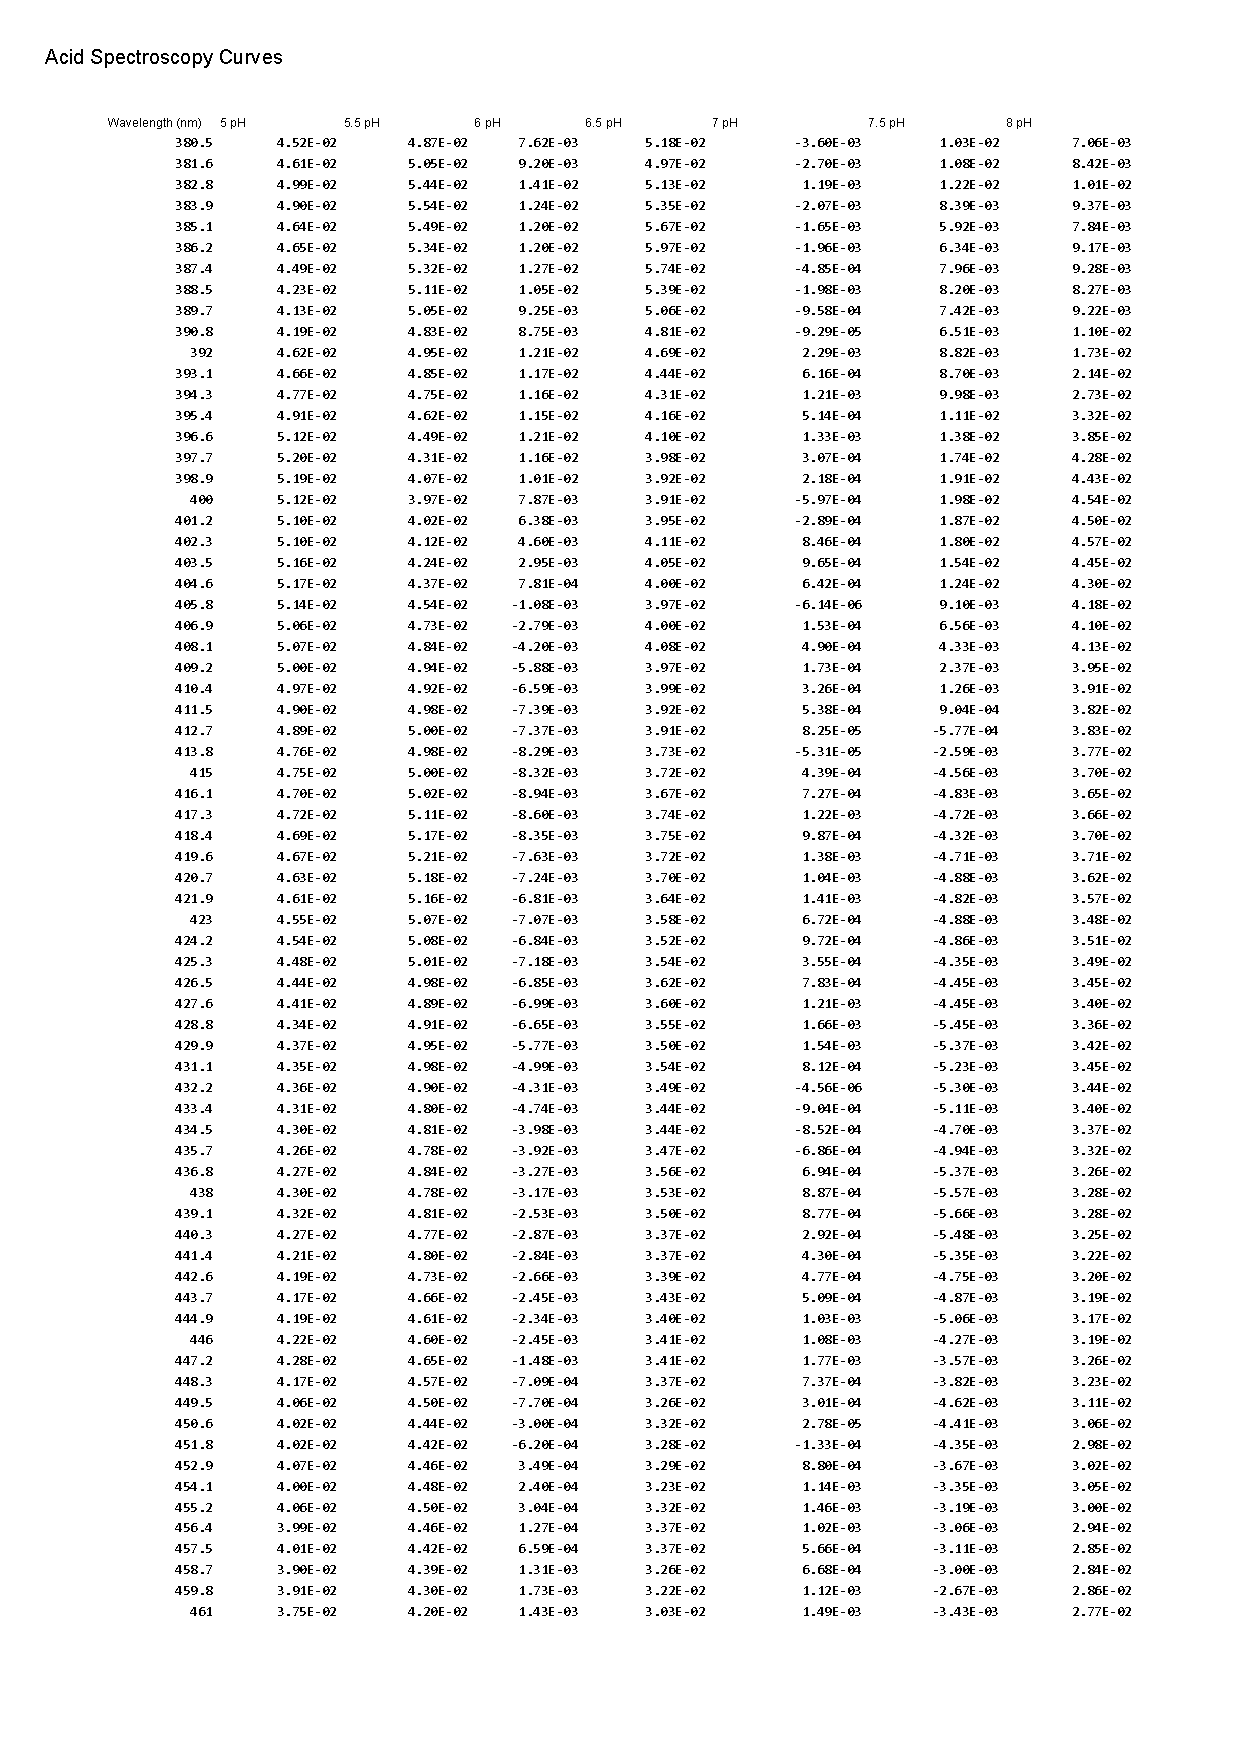
\includepdf[pages=-]{acidtable.pdf}
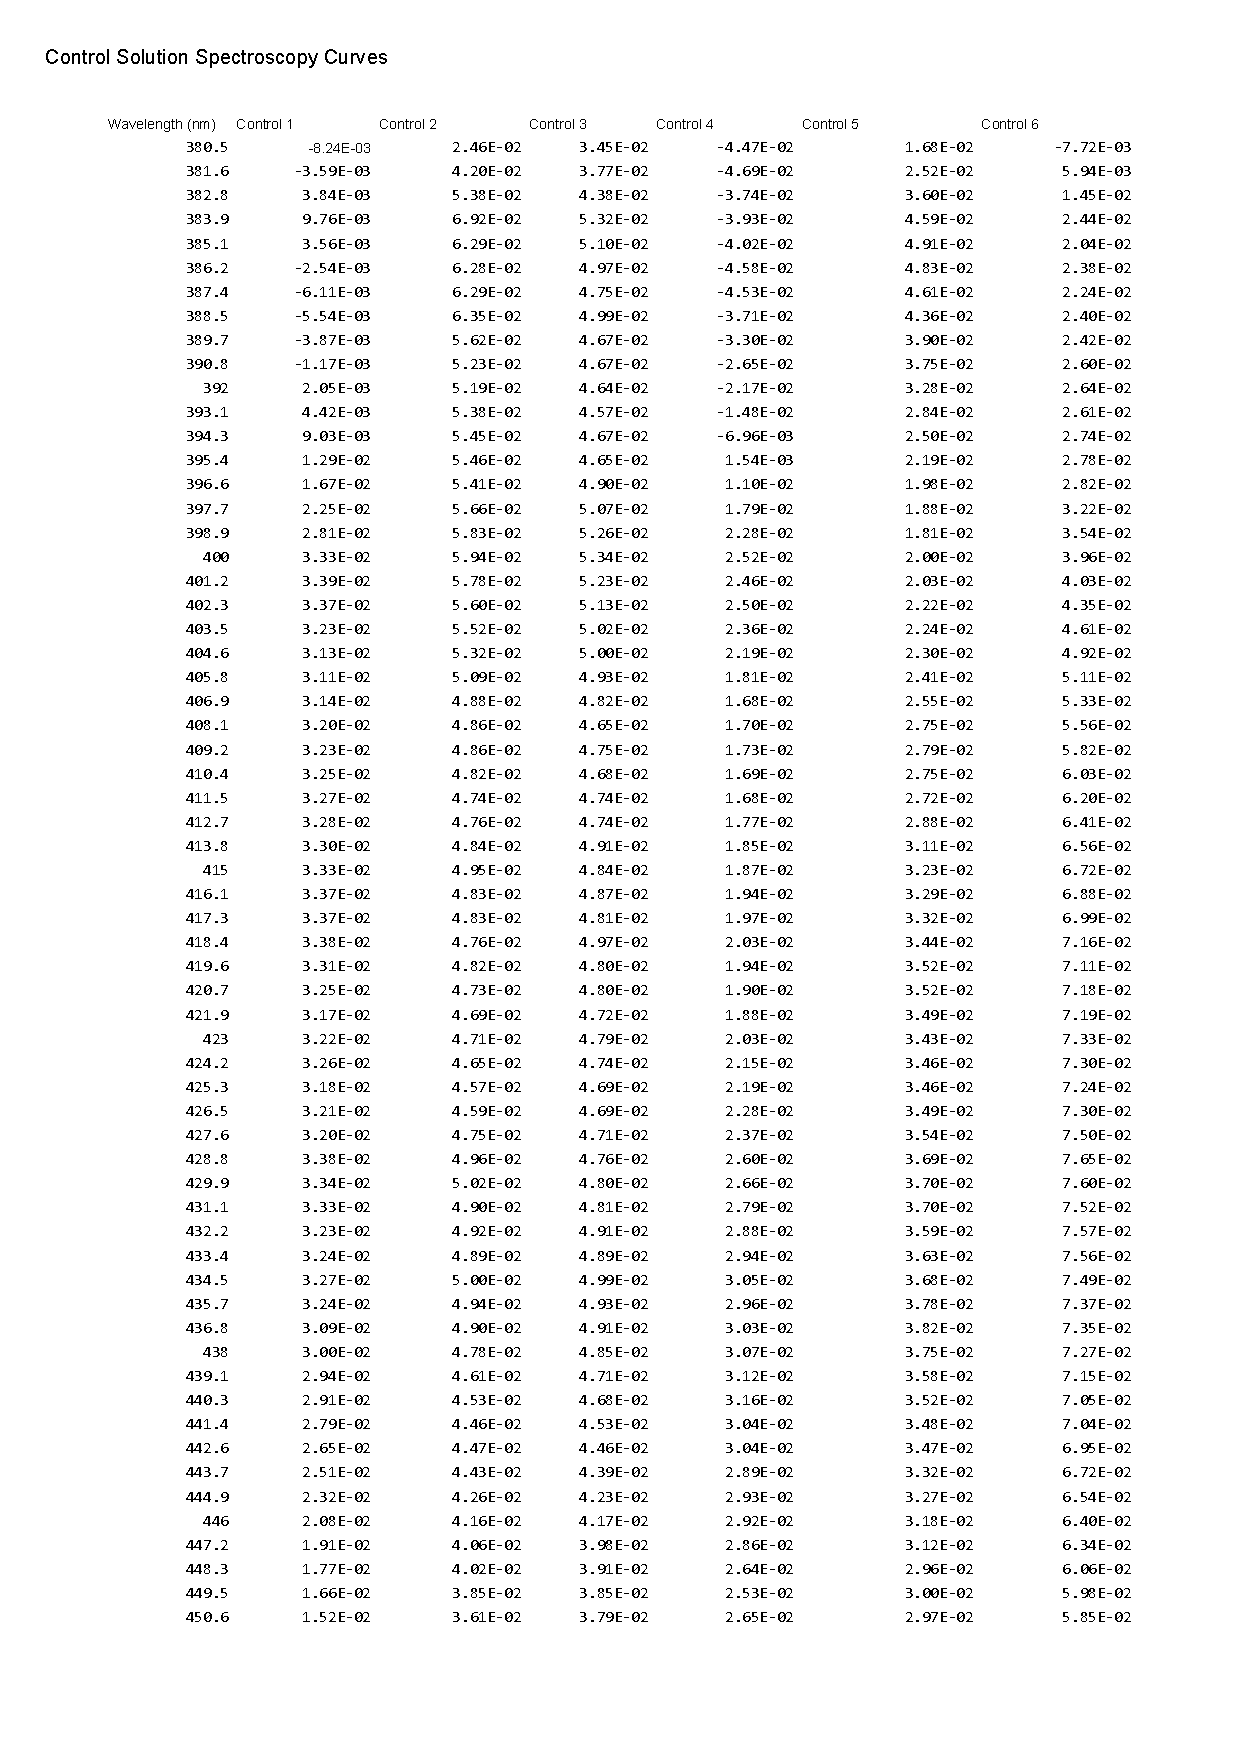
\includepdf[pages=-]{controlstable.pdf}
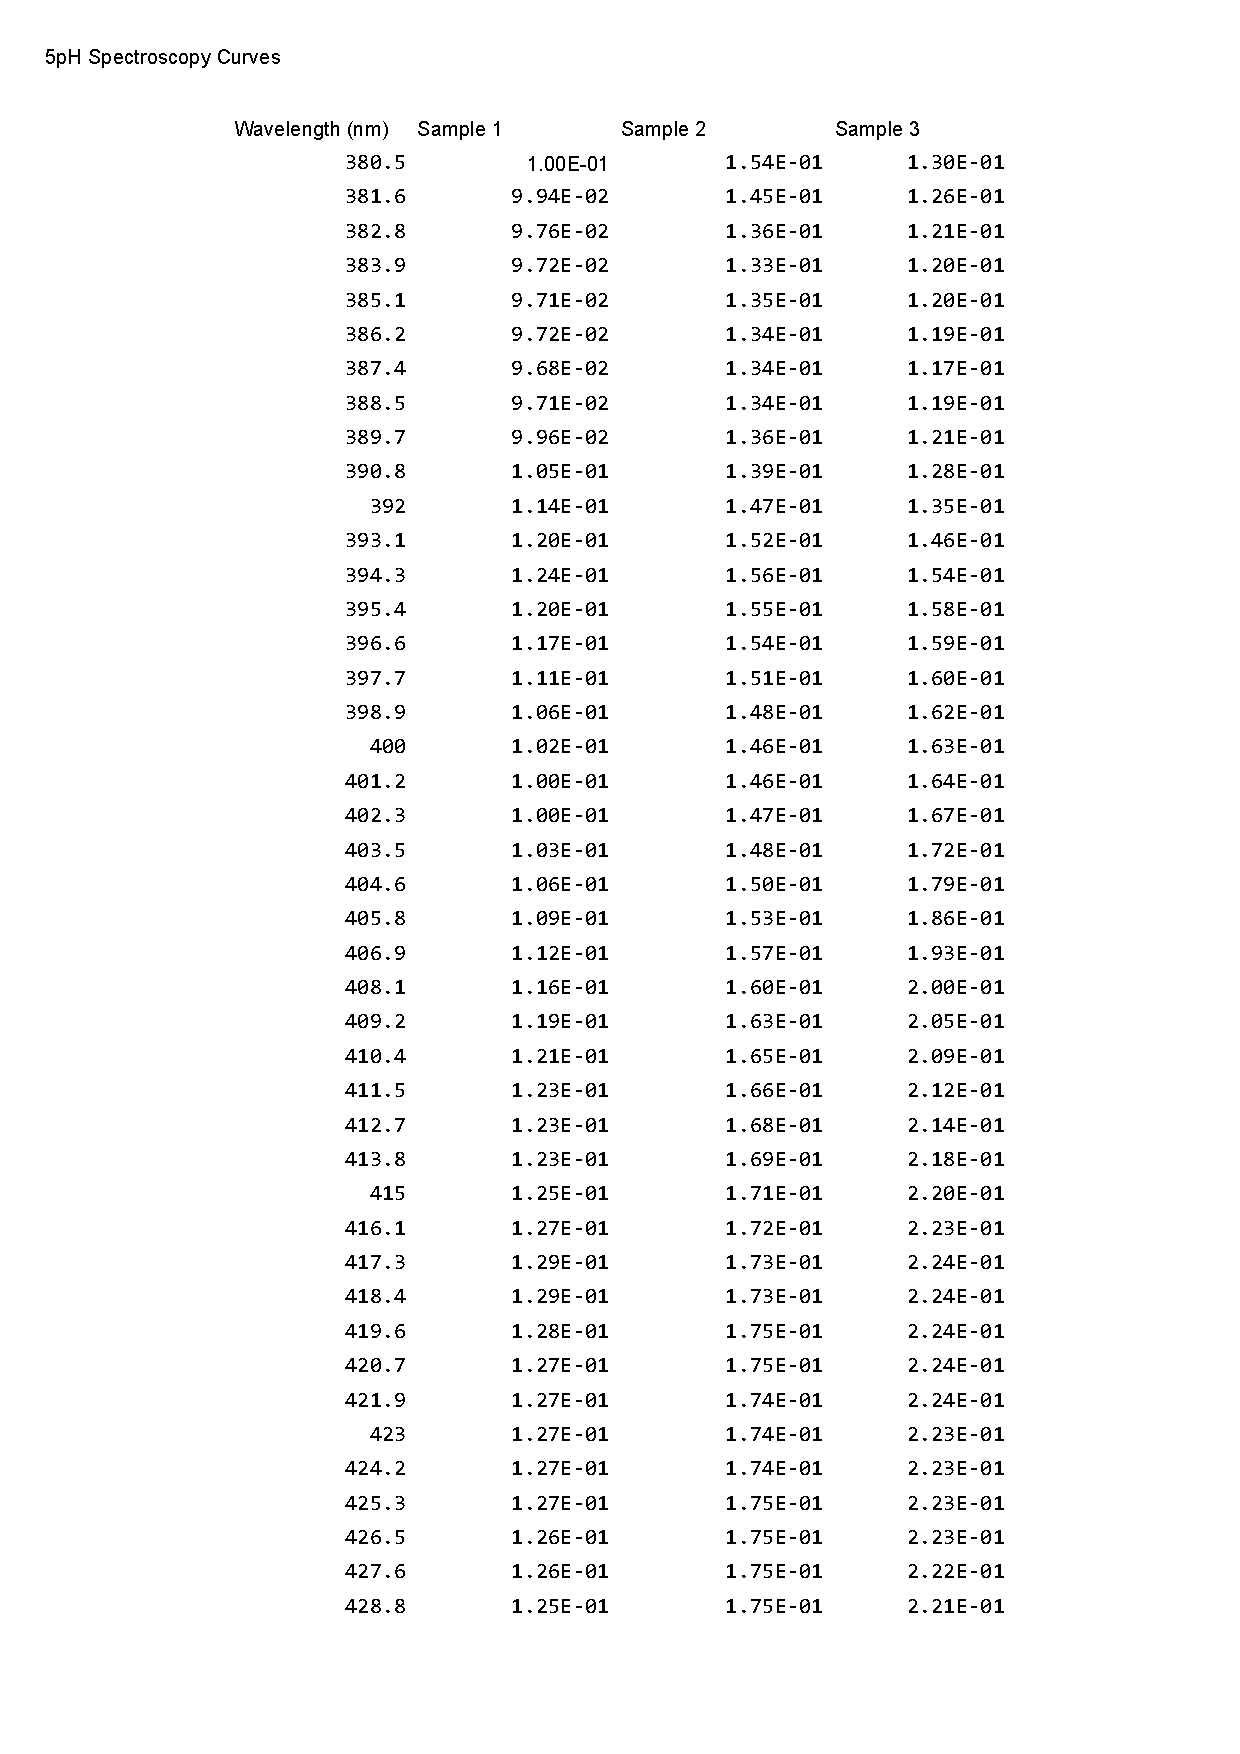
\includepdf[pages=-]{5pH.pdf}
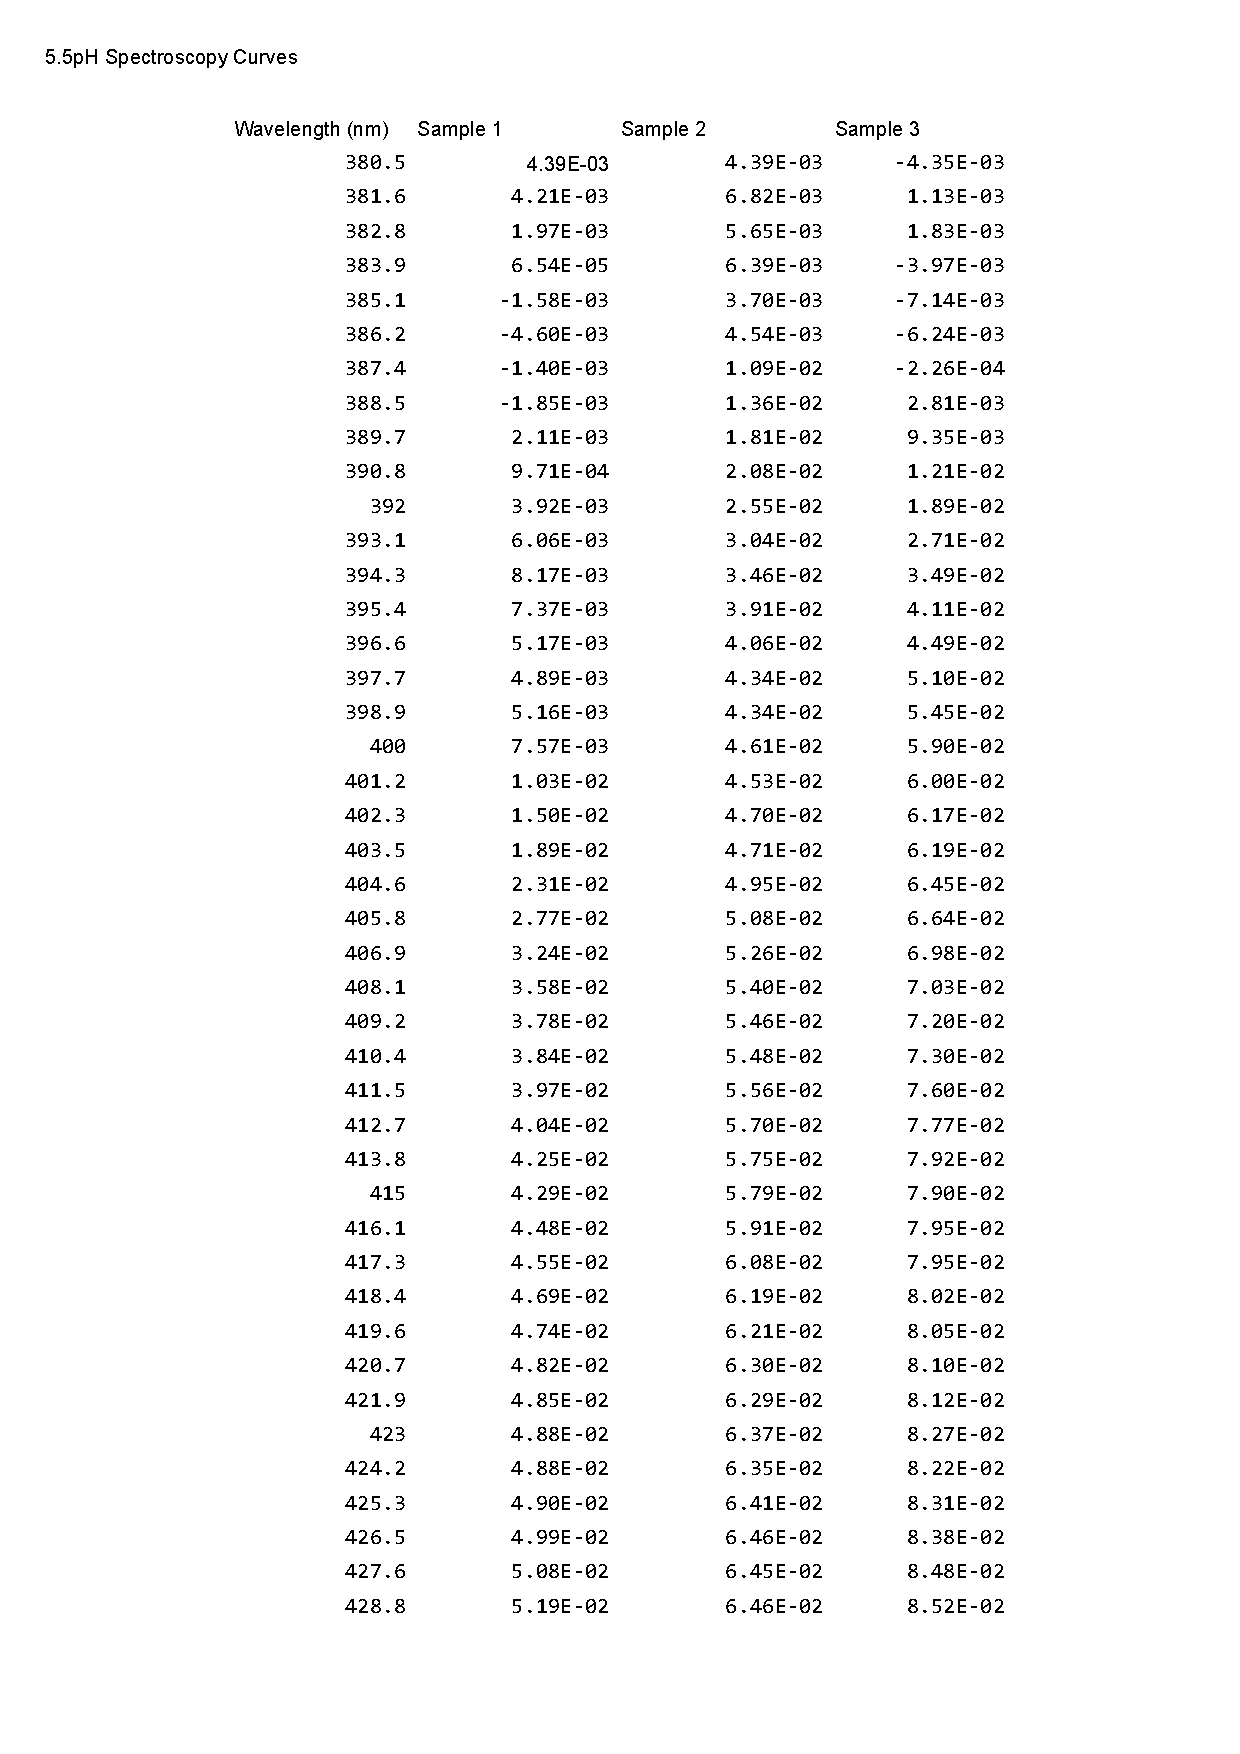
\includepdf[pages=-]{55pH.pdf}
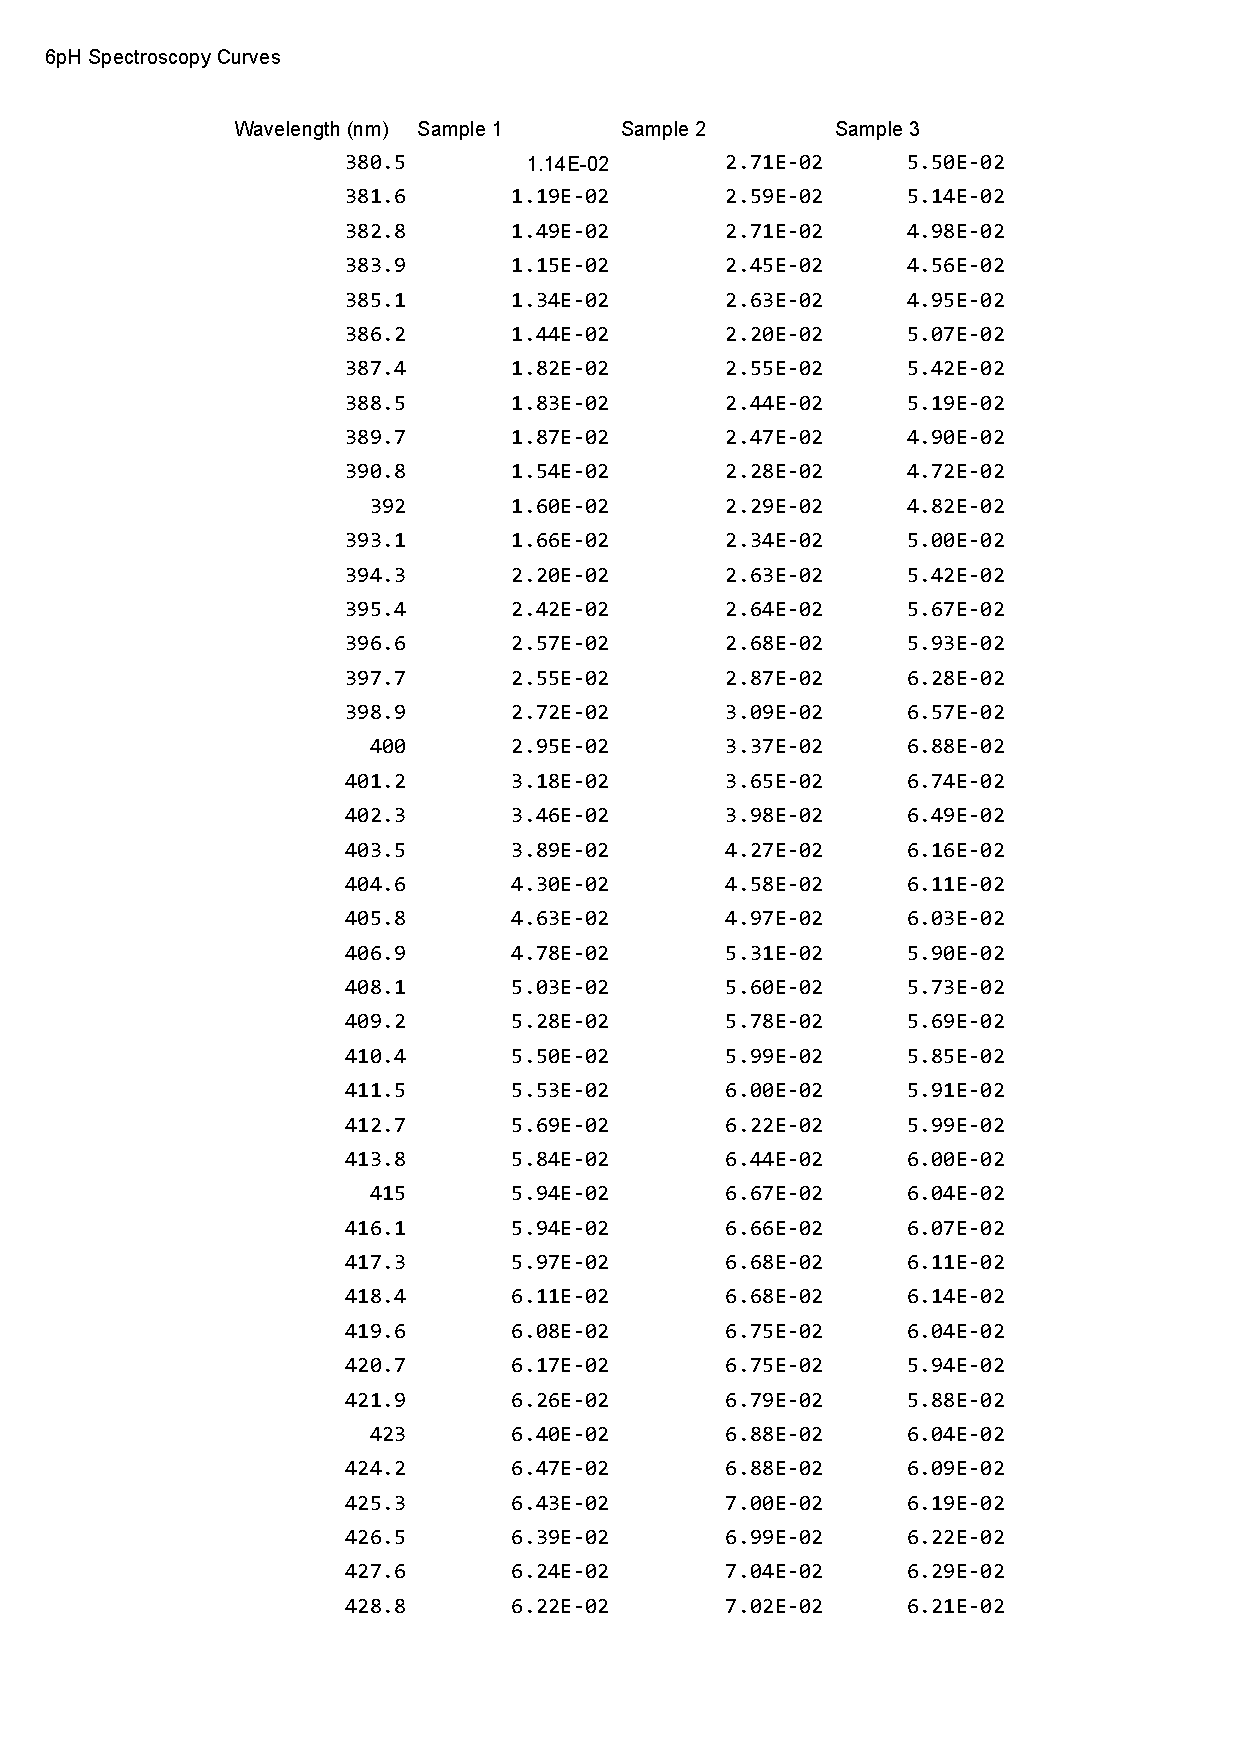
\includepdf[pages=-]{6pH.pdf}
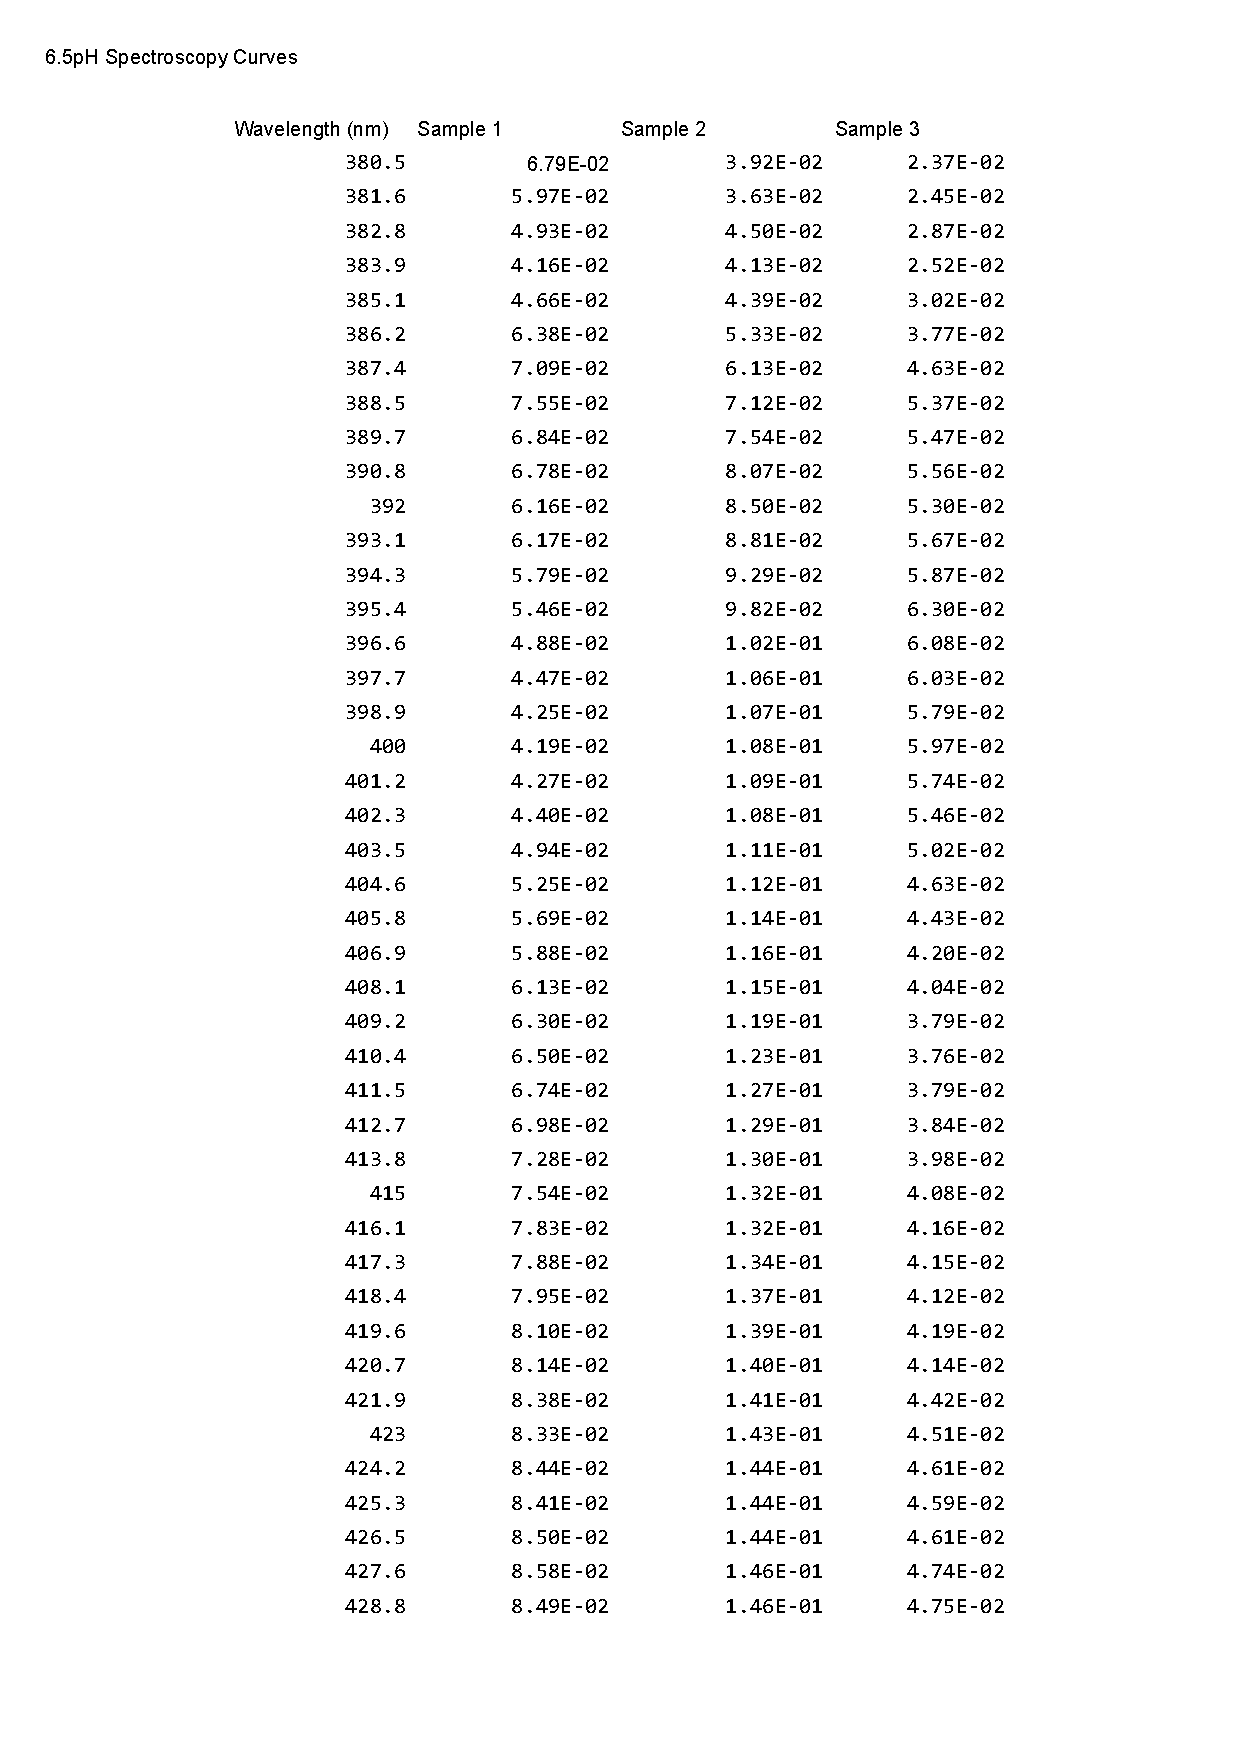
\includepdf[pages=-]{65pH.pdf}
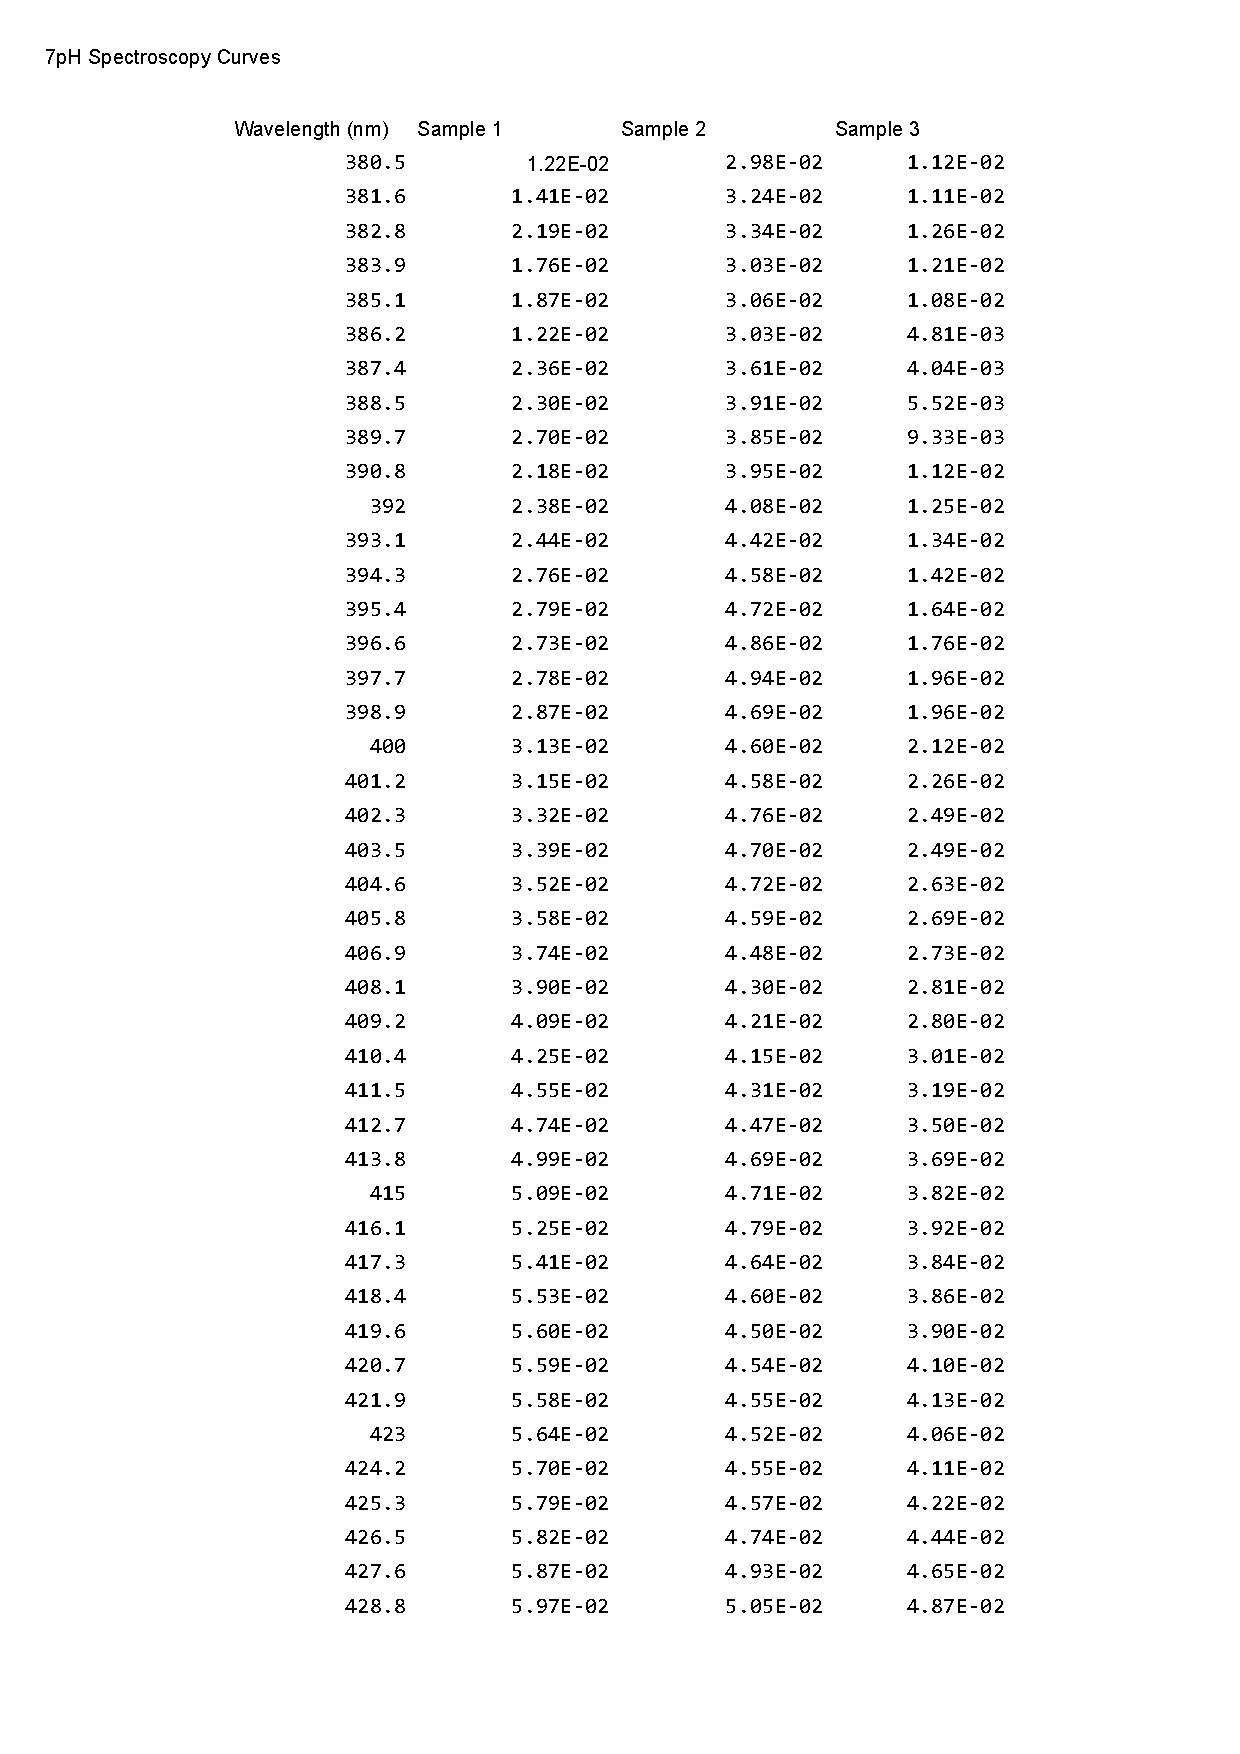
\includepdf[pages=-]{7pH.pdf}
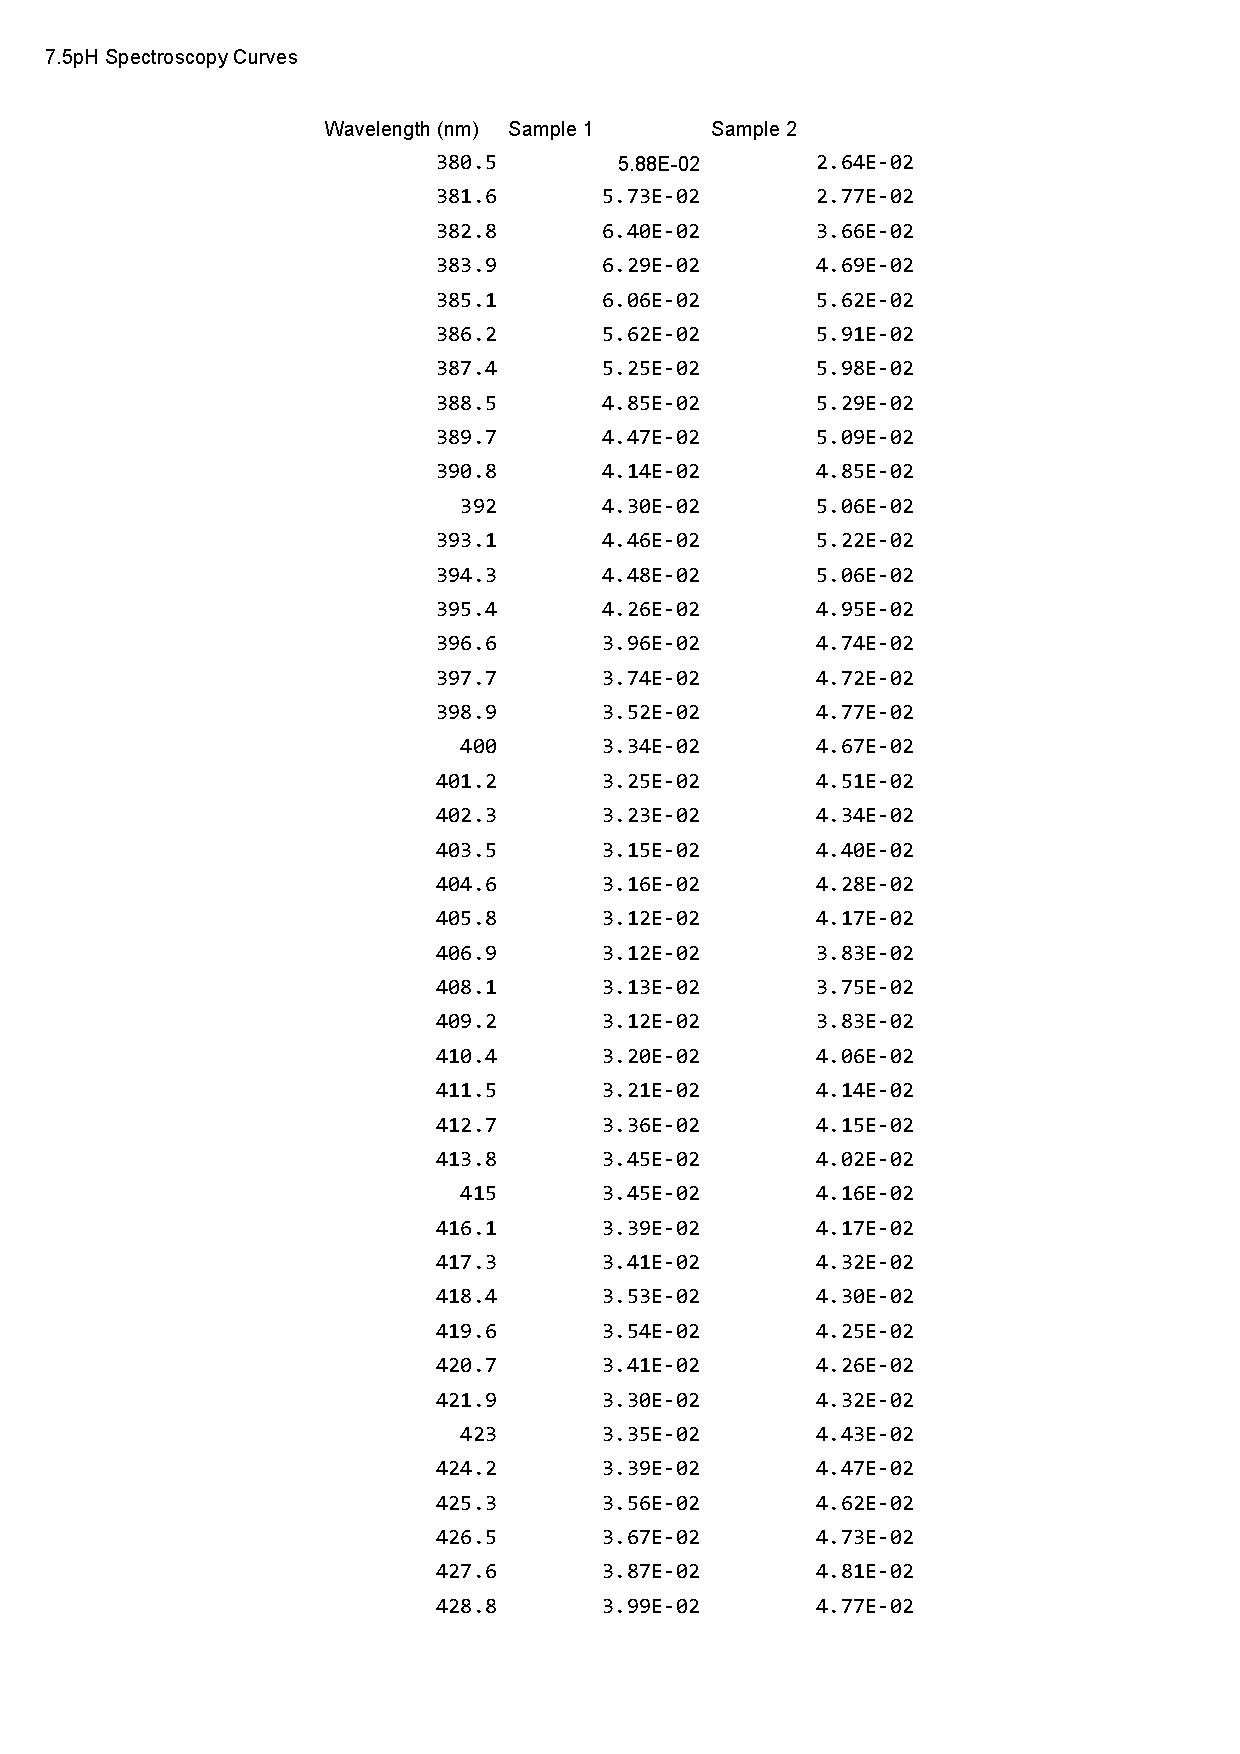
\includepdf[pages=-]{75pH.pdf}
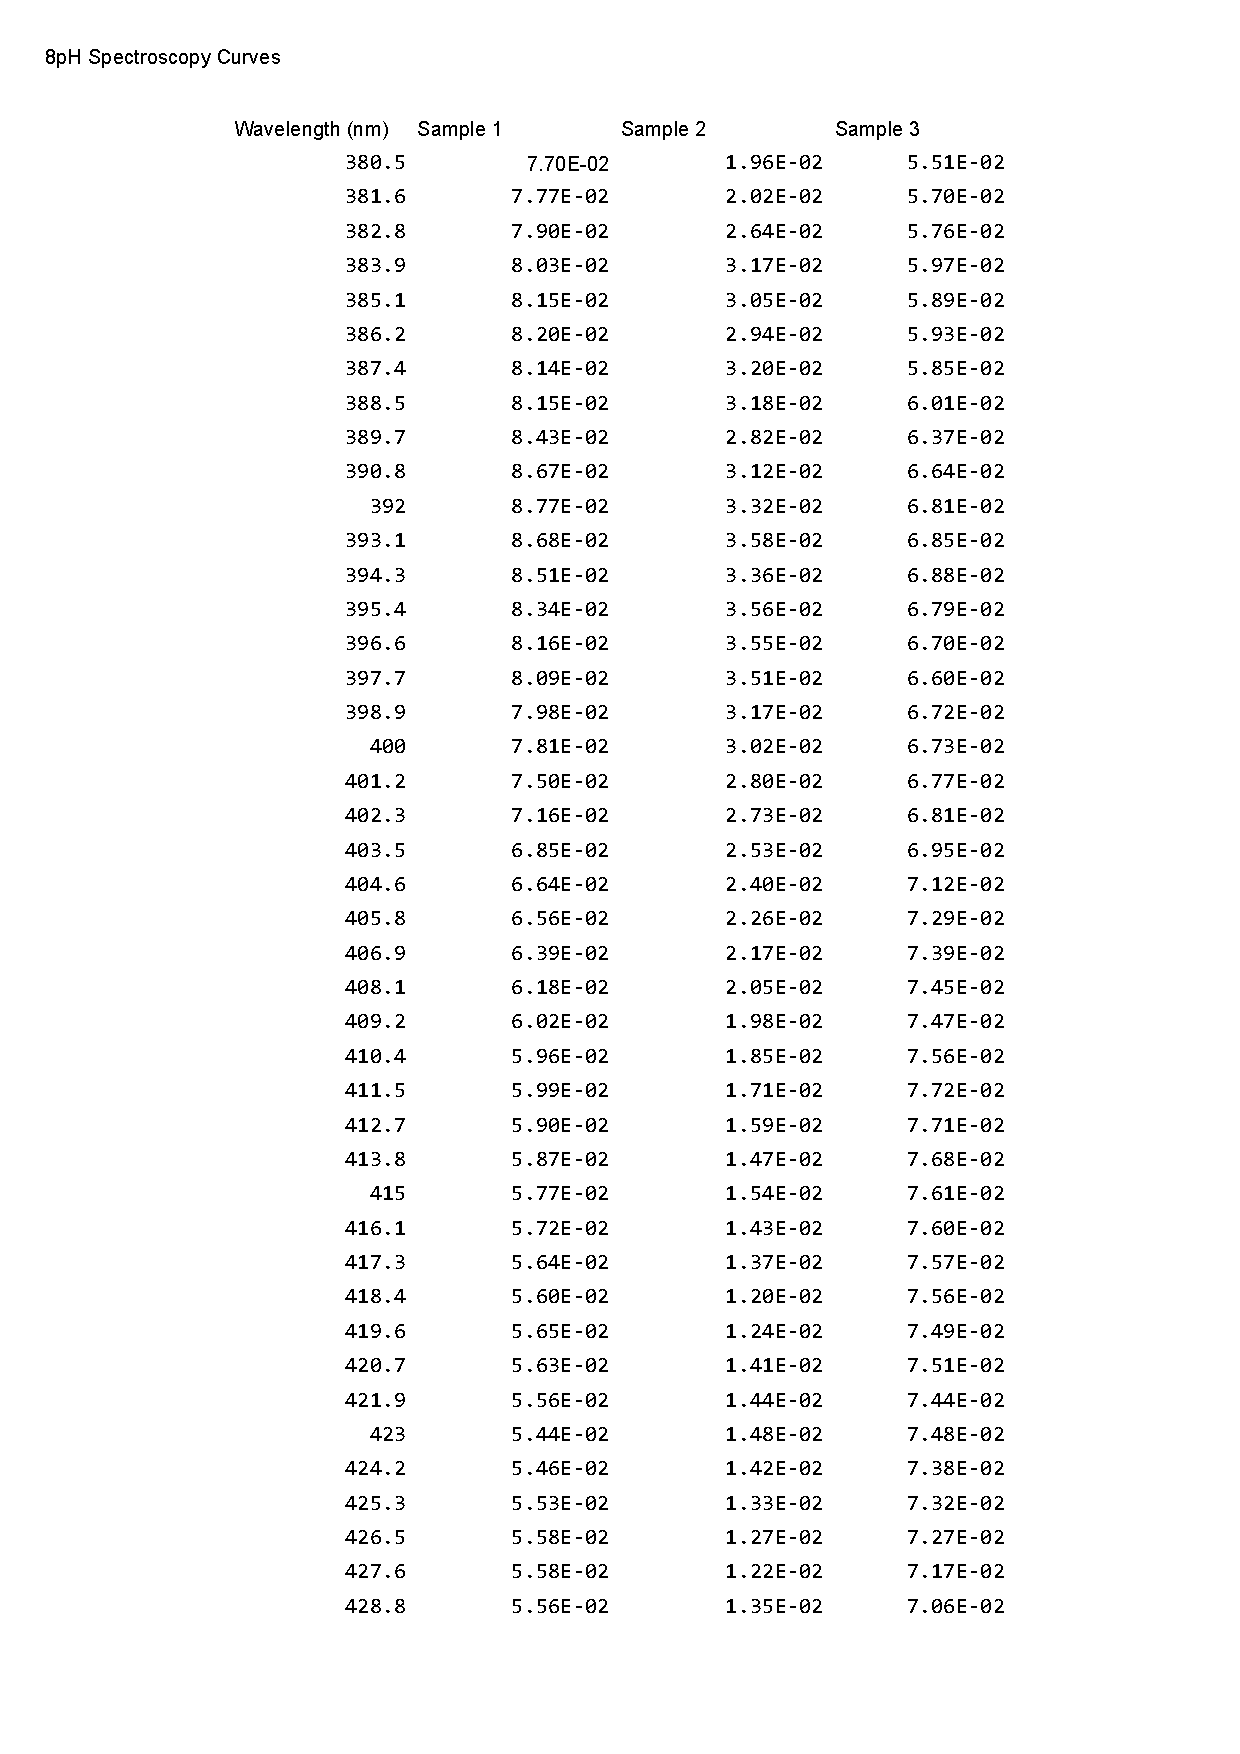
\includepdf[pages=-]{8pH.pdf}
\newpage

\end{document}